\documentclass{article}

\usepackage{amsmath}

\usepackage{tikz}

\usepackage{graphicx}

\usepackage{hyperref}

\usepackage[utf8]{inputenc}

\usepackage{subcaption}

\usepackage{geometry}

\usepackage{multirow}

\usepackage{siunitx}

\usepackage[square,numbers]{natbib}

\usepackage[english]{babel}
%Includes "References" in the table of contents
\usepackage[nottoc]{tocbibind}

\usepackage[parfill]{parskip}

\usepackage[toc,page]{appendix}

\usepackage{tabularx}

\usepackage{booktabs}

\usepackage{pgfplots}

\newcommand{\pvec}[1]{\vec{#1}\mkern2mu\vphantom{#1}}

\DeclareSIUnit{\angstrom}{\textup{\AA}}

\geometry{legalpaper, portrait, margin=1in}

\title{Lab Report}

\author{Jamal Ghaith}
\author{Anas Roumieh}

\date{01.04.2024}

\begin{document}

\begin{titlepage}
	\centering
	{\scshape\LARGE University of Leipzig \par}
	\vspace{1cm}
	{\scshape\ Advanced Labs\par}
	\vspace{1.5cm}
	{\huge\bfseries Lab report\par}
	\vspace{2cm}
	{\huge\bfseries Optical spectroscopy at colour centres and molecules\par}
	\vspace{2cm}
	{\Large Jamal Ghaith 3792970\par}
    {\Large Anas Roumieh 3766647\par}
	\vfill

    {\Large Conducted on: 02.07.2024 \par}
	\vfill
\end{titlepage}


\tableofcontents
\pagenumbering{gobble}
\pagebreak{}
\pagenumbering{arabic}

\section{Introduction}

\subsection{Iodine Molecule Spectra}
\subsubsection{Electronic Transitions}

Electronic transitions in molecules occur when electrons are elevated to higher energy levels. In systems with multiple electrons, only those in non-closed shells are taken into account because their orbital angular momentum does not cancel out, unlike in closed shells. 
The orbital angular momentum of these electrons in non-closed shells contributes to the total orbital angular momentum of the electron shell, resulting in values that are integer multiples of $\hbar$. These are denoted by Greek letters $\Sigma$, $\Pi$, $\Delta$, $\Phi$ instead of numbers. Quantum mechanics imposes a selection rule that governs these electronic transitions:

\begin{equation*}
	\Delta \Lambda = 0, \pm 1
\end{equation*}

The same principle applies to the total spin $S$, which is determined by the spins of the electrons in partially filled shells. Due to the interaction between spin and orbital angular momentum, the energy levels associated with the orbital angular momentum are split into $2S + 1$ values, referred to as multiplicity $M$. 
When considering diatomic molecules, symmetry must also be considered, unlike in atoms. It is essential to determine whether a state function, when inverted at the center of symmetry, is symmetric or antisymmetric relative to its initial form. If a phase shift occurs at the boundary, the function is labeled as odd "u"; otherwise, it is labeled as even "g". 
Additionally, a mirror-symmetric function is denoted with a "$+$", while an antisymmetric function is indicated with a "$-$". This leads to the following format for the complete description of the electronic state of a molecule:

\begin{equation*}
	\label{eq:state}
	^{M}\Lambda_{g,u}^{\pm}
\end{equation*}

\subsubsection{Vibrational Transitions}

In addition, the interactions between the atoms within a molecule must be considered.

\begin{figure}[h!]
	\centering
	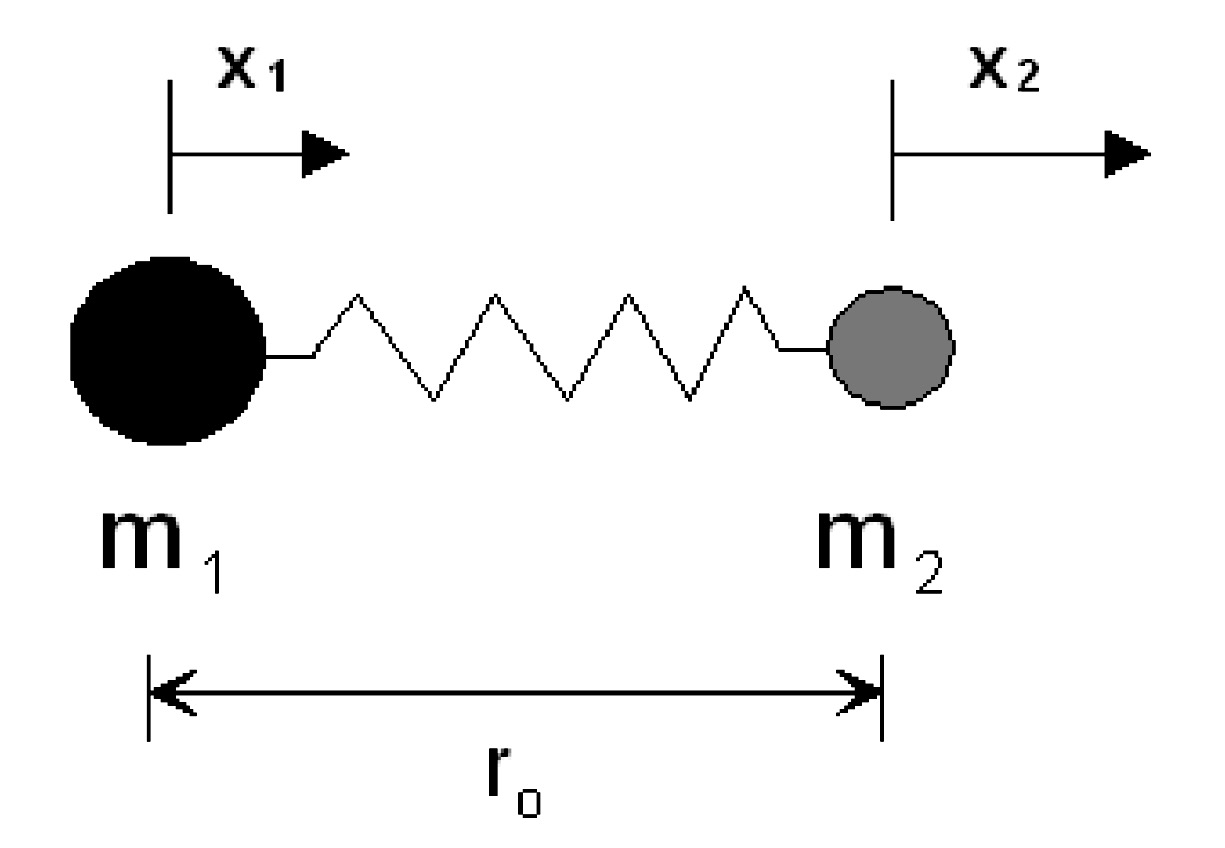
\includegraphics[width=0.7\textwidth]{Figures/Introduction/Oscillator.jpg}
	\caption{From \cite{riede_optical}}
\end{figure}


To do this, the harmonic oscillator model is employed, and the equations of motion for a diatomic molecule are derived by considering the forces involved. These forces can be transformed using $x = x_1 - x_2$ into the following equations:

\begin{equation*}
m_1 \ddot{x}_1 = -k(x_1 - x_2) 
\end{equation*}
\begin{equation*}
m_2 \ddot{x}_2 = -k(x_2 - x_1) 
\end{equation*}
\begin{equation*}
\ddot{x} = -\frac{k}{\mu}x 
\end{equation*}

The resonance wavenumber of such a harmonic oscillator is then given by:

\begin{equation*}
\bar{\nu}_s = \frac{1}{2\pi c}\sqrt{\frac{k}{\mu}} 
\end{equation*}

To calculate the energy levels, one solves the Schrödinger equation for the potential

\begin{equation*}
U = 2\pi^2c^2\bar{\nu}^2\mu x^2
\end{equation*}

which is derived from the restoring force using the relation

\begin{equation*}
-\frac{dU}{dx} = F = -\frac{k}{x} 
\end{equation*}

and the solution

\begin{equation*}
x = x_0 \sin(2\pi c\bar{\nu}_s t) 
\end{equation*}

yields discrete energy levels

\begin{equation*}
E(n) = h c \bar{\nu}_s \left(n + \frac{1}{2}\right); \quad n = 0, 1, 2, \ldots
\end{equation*}

with the selection rule

\begin{equation*}
\Delta n = \pm 1. 
\end{equation*}

Experimentally, however, the spacings between vibrational energy levels are not constant, decreasing at higher $n$. Additionally, it is known that a molecule will dissociate at sufficiently large bond lengths, and the strong nuclear force must be considered at very short distances. Therefore, it is advisable to transition from the harmonic oscillator model to the Morse potential.

\begin{equation*}
U = E_D a^2 x^2
\end{equation*}

this is valid for small $x$, $E_D$ is the dissociation energy and 

\begin{equation*}
a = 2\pi \bar{\nu}_s c \sqrt{\frac{\mu}{2E_D}} = \omega_s \sqrt{\frac{\mu}{E_D}}
\end{equation*}

The constant $a$ is a characteristic parameter of the molecule. Solving the Schrödinger equation with this potential yields the approximate energy eigenvalues:

\begin{equation*}
E(n) = h c \bar{\nu} \left[ \left(n + \frac{1}{2}\right) - \gamma_e \left(n + \frac{1}{2}\right)^2\right]
\end{equation*}

where $\gamma_e$ is the anharmonicity constant. This leads to the following diagram for the anharmonic oscillator.

\begin{figure}[h!]
	\centering
	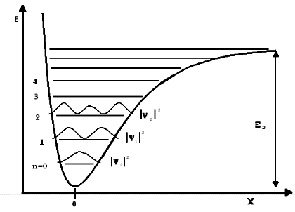
\includegraphics[width=0.7\textwidth]{Figures/Introduction/Anharmonic.jpg}
	\caption{From \cite{riede_optical}}
\end{figure}

\pagebreak{}

\subsubsection{Combined Transitions}

When combining the results of the isolated observations of electronic and vibrational transitions, it is important to also consider the coupling effect between them. The equilibrium bond length for vibrations depends on the electronic state, which can lead to different scenarios: the binding energy may remain constant with respect to distance (a), increase (b), or decrease (c) in the excited state. The Franck-Condon principle is also applicable, stating that electronic transitions occur much faster than molecular vibrations, which is why the transitions are depicted as vertical lines in the diagram.

\begin{figure}[h!]
	\centering
	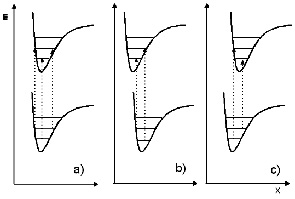
\includegraphics[width=0.7\textwidth]{Figures/Introduction/Combined.jpg}
	\caption{From \cite{riede_optical}}
\end{figure}

For the transition energy between two levels $n'$ and $n''$ this results in

\begin{align*}
	\Delta E(n', n'') = E(n') - E(n'') &= E_{\text{elektr}} + hc\bar{\nu}_s' \left(n' + \frac{1}{2}\right) 
	- hc\bar{\nu}_s'' \left(n'' + \frac{1}{2}\right) \nonumber \\
	&\quad - hc\bar{\nu}_s'\gamma'_e \left(n' + \frac{1}{2}\right)^2 
	+ hc\bar{\nu}_s''\gamma''_e \left(n'' + \frac{1}{2}\right)^2
\end{align*}
	
However, to dissociate the molecule, it is not sufficient to provide it with the energy $E_D$, as transitions with large $\Delta n$ are very unlikely.
	
\begin{figure}[h!]
	\centering
	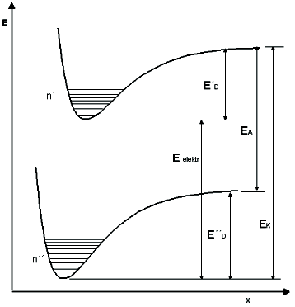
\includegraphics[width=0.7\textwidth]{Figures/Introduction/Energies.png}
	\caption{Definiton of transition energies. \cite{riede_optical}}
	\label{fig:Dissociation}
\end{figure}

However, if an electron is excited, the transition probability increases, and the transition energy between states with $n'$ and $n''$ results in

\begin{equation}
	\label{eq:Iodinefit}
	\Delta E = E_{electronic} + E'_S \left(n' + \frac{1}{2}\right) - E'_S y'_e\left(n' + \frac{1}{2}\right)^2
\end{equation}

For high $n'$, the values converge towards $E_K$, and two lines with a quantum difference of $N$ differ by

\begin{equation*}
\Delta(\Delta E) = E_S' \left(n' + \frac{1}{2} + N\right) - E_S' \left(n' + \frac{1}{2}\right) - E_S' \gamma_e' \left(n' + \frac{1}{2} + N\right)^2 + E_S' \gamma_e' \left(n' + \frac{1}{2}\right)^2
\end{equation*}

which simplifies to:

\begin{equation*}
\Delta(\Delta E) = E_S' N - E_S' \gamma_e' N(2n' + N + 1) = E_S' \left(1 - \gamma_e' (n + 1)\right)
\end{equation*}

for $N = 1$, where the distance between two neighboring line spacings depends linearly on $n'$ and therefore

\begin{equation*}
\Delta(\Delta E)(n') - \Delta(\Delta E)(n' + 1) = -2E_S' \gamma_e' = \text{const.}
\end{equation*}

As this distance approaches zero for $E = E_K$, the following also results in

\begin{equation}
	\label{eq:ne}
	n'_E = \frac{1}{2y'_e} -1
\end{equation}

which can be used to find $n'_E$.

if in Equation \ref{eq:Iodinefit} $n' = n'_E$, then:

\begin{equation}
	\label{eq:convergence}
	\Delta E = E_K = E_{electronic} + E'_S \left(n'_E + \frac{1}{2}\right) - E'_S y'_e\left(n'_E + \frac{1}{2}\right)^2
\end{equation}

This can be used to calculate $E_{\text{electronic}}$, where $E_A$ and $E'_S$ are assumed to be known. The following values apply: $E'_S = 0.0159$ eV and $E_A = 0.94$ eV.

\pagebreak{}

\subsection{Color Centers}

\subsubsection{General}

In ionic crystals, particularly alkaline halides, electrons are strongly localized. These materials exhibit a wide energy gap between the valence and conduction bands, typically ranging from 5 to 12 eV. As a result, visible light, which has an energy range of about 1.5 to 3.5 eV, is insufficient to excite an electron from the valence band to the conduction band. As a result, pure ionic crystals are transparent and electrically insulating. However, thermal or chemical treatment, as well as exposure to x-rays or ultraviolet light, can induce point defects in these alkaline halides. These defects, such as ion vacancies, interstitials, or impurity atoms, become incorporated into the crystal lattice. They can trap electrons in bound states that are less localized than in the unperturbed lattice. These bound states fall within the forbidden energy gap, often within the visible spectral range for alkaline halides. This causes the crystals to exhibit a characteristic color—NaCl appears red, KBr appears blue—and these defects are known as color centers. There is a variety of color centers, each with different designations for historical reasons, as illustrated in Fig. \ref{fig:colour centres} \cite{riede_optical}.

\begin{figure}[h!]
    \centering
    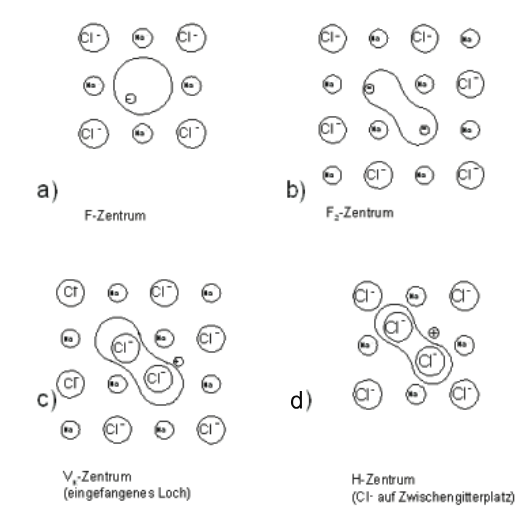
\includegraphics[width=0.4\linewidth]{Figures/Introduction/1.png}
    \caption{The defect structure in alkaline halides: (a) Halogen ion vacancy with a
trapped electron, F-centre (b) two neighbouring colour centres, (c) self-trapped hole, (d)
halogen ion on a interstitial site, Frenkel pair}
    \label{fig:colour centres}
\end{figure}

A colour centre (F-centre) is an anion vacancy (halogen vacancy) with a trapped electron (see Fig. \ref{fig:colour centres}). To create F-centres, gamma rays, X-rays, electron beams, or ultraviolet irradiation, as well as annealing the crystal in alkali vapor can be used. The energy from these radiations excites an electron from a halogen ion across the band gap, forming an exciton with a hole in the valence band. The neutral halogen atom is no longer firmly bound to its lattice site; it moves and creates a molecule-like state with a neighboring halogen ion, where the hole attaches. This configuration is known as the $V_K$ centre. The energy released during the exciton recombination is sufficient to generate a Frenkel pair (H-centre) from the $V_K$ centre, meaning the halogen ion vacancy moves to an interstitial site, leaving behind a vacancy at the original halogen ion site. Consequently, both an F-centre and an H-centre are formed, with the electron attaching to the F-centre. This process is energetically more efficient than directly shifting the halogen ion to an interstitial site. EPR experiments have indicated that the F-centre has a spin of 1/2, supporting the presence of a trapped electron at the halogen vacancy. Optical transmission studies of F-centres revealed a broad absorption band in the visible spectrum, associated with the electronic transition from the ground state to the first excited state. This absorption band is illustrated schematically in Fig. \ref{fig:peak}. The full width at half maximum (FWHM) of this band is represented as $\Delta E_H$. The transition energy, denoted as $E_m$, is related to the wavelength $\lambda_m$ as follows:

\begin{equation*}
    E = \frac{hc}{\lambda}
\end{equation*}

\begin{figure}[h!]
    \centering
    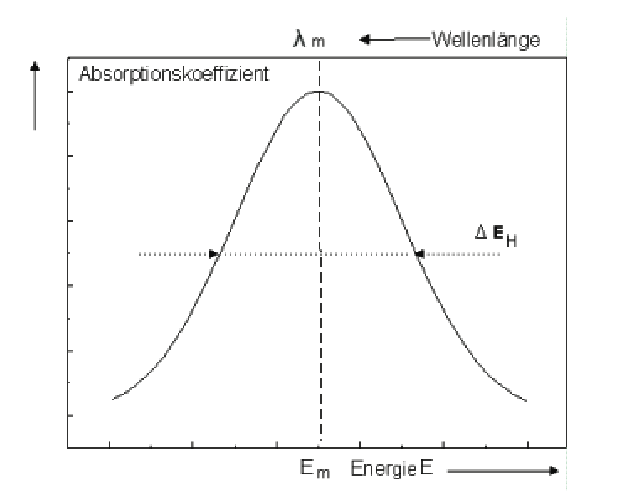
\includegraphics[width=0.4\linewidth]{Figures/Introduction/2.png}
    \caption{Schematic absorption line of an F-centre.}
    \label{fig:peak}
\end{figure}

\pagebreak{}

\subsubsection{F-centres classically}
The traditional model of the F-centre, such as in NaCl, assumes that the Cl$^-$  vacancy leads to a positive charge on the surrounding Na$^+$ ions. This positive charge, denoted as $e^+$, is conceptualized as being spread uniformly over the surface of a sphere with the same volume as a cube with edge length $d'$. According to Fig. \ref{fig:classical}, the radius $R$ of this sphere is determined by:

\begin{equation*}
    d'^3 = \frac{4\pi}{3} R^3
\end{equation*}

with 

\begin{equation*}
    d' = \sqrt{2}d = \frac{\sqrt{2}}{2}a
\end{equation*}

Hence we get: 

\begin{equation*}
    R^3 = \frac{3\sqrt{2}}{16\pi}a^3
\end{equation*}

The electron trapped at the F-centre, carrying a charge of $e^-$, is now situated within the uniformly distributed charge density $\rho$ at position $r$. The electron experiences a radial electric field $E = Er$, which is generated by the uniformly charged sphere. Due to the symmetry of the charge distribution, this electric field has only a radial component. The total positive charge is represented by: 

\begin{equation*}
    e^{+}=\int \rho \mathrm{d} V=\rho \frac{4 \pi}{3} R^3
\end{equation*}

and the Maxwell's equation: 

\begin{equation*}
    \nabla D = \rho
\end{equation*}

we get the $E_r$ field: 

\begin{equation*}
    E_r = \frac{\rho}{3\epsilon \epsilon_0} r = \frac{e^+}{4\pi \epsilon \epsilon_0}\frac{r}{R^3}
\end{equation*}

yielding the Coulomb force: 

\begin{equation*}
    F_r = m \ddot{r}=-\frac{e^2}{4 \pi \epsilon \epsilon_0} \frac{r}{R^3} 
\end{equation*}

and by transforming it into an oscillation equation we also get the angular frequency: 

\begin{equation*}
    \omega=\frac{e^2}{4 \pi \epsilon \epsilon_0 m R^3}
\end{equation*}

And finally the excitation energy: 

\begin{equation*}
    E=\frac{\hbar e}{\left(4 \pi \epsilon \epsilon_0\right)^{1/2} R^{3/2}}
\end{equation*}

Replacing $R$ by the lattice constant $a$ one finally obtains:

\begin{equation*}
    E=\frac{h e}{\pi\left(3 \sqrt{2} \epsilon \epsilon_0 a^3\right)^{1 / 2}} .
\end{equation*}

The excitation energy of the oscillator, which determines the peak of the absorption line, corresponds to the transition energy $E_m$. Therefore, the classical model of the F-centre can be described as a harmonic oscillation of the trapped electron within the electric potential of a uniformly positively charged sphere.

\begin{figure}[h!]
    \centering
    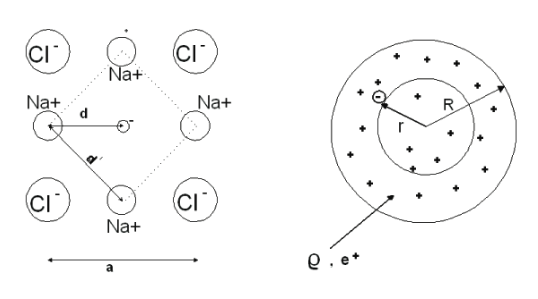
\includegraphics[width=0.3\linewidth]{Figures/Introduction/3.png}
    \caption{Classical model of the F-centre}
    \label{fig:classical}
\end{figure}

\pagebreak{}

\subsubsection{Quantum Mechanical Description}

For the quantum mechanical consideration of color centers, a three-dimensional box potential with edge lengths $a$, $b$, and $c$ and infinitely high walls is assumed. Within this box, the following results:

\begin{equation*}
-\frac{\hbar^2}{2m} \Delta \Psi = E \Psi, 
\end{equation*}

where

\begin{equation*}
\Delta \Psi = -\alpha \Psi, 
\end{equation*}

and

\begin{equation*}
\alpha = \frac{2mE}{\hbar^2}.
\end{equation*}

Since the Laplacian operator is a sum of second derivatives in the three spatial directions, the product function

\begin{equation*}
\Psi = \Psi_1(x) \Psi_2(y) \Psi_3(z), 
\end{equation*}

is used. Applying the Laplacian operator results in

\begin{equation*}
	\Delta \left( \Psi_1(x) \Psi_2(y) \Psi_3(z) \right) = -\alpha \Psi_1(x) \Psi_2(y) \Psi_3(z).
\end{equation*}
	

Dividing by the product function gives:

\begin{equation*}
\frac{1}{\Psi_1(x)} \frac{\partial^2 \Psi_1(x)}{\partial x^2} + \frac{1}{\Psi_2(y)} \frac{\partial^2 \Psi_2(y)}{\partial y^2} + \frac{1}{\Psi_3(z)} \frac{\partial^2 \Psi_3(z)}{\partial z^2} = -\alpha. 
\end{equation*}

With $x$, $y$, and $z$ as independent variables and $\alpha$ as a constant, each term must be a constant:

\begin{equation*}
\frac{1}{\Psi_1(x)} \frac{\partial^2 \Psi_1(x)}{\partial x^2} = -\alpha_1, 
\end{equation*}
\begin{equation*}
\frac{1}{\Psi_2(y)} \frac{\partial^2 \Psi_2(y)}{\partial y^2} = -\alpha_2, 
\end{equation*}
\begin{equation*}
\frac{1}{\Psi_3(z)} \frac{\partial^2 \Psi_3(z)}{\partial z^2} = -\alpha_3. 
\end{equation*}

Thus,

\begin{equation*}
\alpha = \alpha_1 + \alpha_2 + \alpha_3. 
\end{equation*}

This decouples the coordinates, allowing the differential equations to be solved separately using the harmonic approach:

\begin{equation*}
\Psi_1(x) = A_1 \sin(\beta_1 x), 
\end{equation*}
\begin{equation*}
\Psi_2(y) = A_2 \sin(\beta_2 y), 
\end{equation*}
\begin{equation*}
\Psi_3(z) = A_3 \sin(\beta_3 z). 
\end{equation*}

By inserting these wave functions into the equation, we get:

\begin{equation*}
	\alpha_i = \frac{2m \beta_i^2}{\hbar^2}, \quad i = 1, 2, 3.
\end{equation*}
	

Thus, the boundary conditions are $\Psi_1(x = 0) = \Psi_1(x = a) = 0$ (analogous for the other two directions),

\begin{equation*}
\beta_1 = \frac{n_1 \pi}{a}, \quad \beta_2 = \frac{n_2 \pi}{b}, \quad \beta_3 = \frac{n_3 \pi}{c}, 
\end{equation*}

where $n_1$, $n_2$, and $n_3$ are positive integers.

The energy eigenvalues are then:

\begin{equation*}
E = \frac{\hbar^2 \pi^2}{2m} \left( \frac{n_1^2}{a^2} + \frac{n_2^2}{b^2} + \frac{n_3^2}{c^2} \right). 
\end{equation*}

Finally, the normalization condition:

\begin{equation*}
\int_0^a \int_0^b \int_0^c |\Psi(x, y, z)|^2 \, dx \, dy \, dz = 1 
\end{equation*}

leads to the final wave function:

\begin{equation*}
\Psi = \frac{8}{abc} \sin \left( \frac{n_1 \pi x}{a} \right) \sin \left( \frac{n_2 \pi y}{b} \right) \sin \left( \frac{n_3 \pi z}{c} \right). 
\end{equation*}

The associated energy is:

\begin{equation*}
	E_{n_1, \ n_2, \ n_3} = E_0 \left( \frac{n_1^2}{a^2} + \frac{n_2^2}{b^2} + \frac{n_3^2}{c^2} \right),
\end{equation*}

which agrees well with experimental results. For the transition from the ground state to the first excited state, the following result is obtained:

\begin{equation*}
\Delta E = \frac{3h^2}{8ma^2}. 
\end{equation*}

\begin{figure}[h]
    \centering
    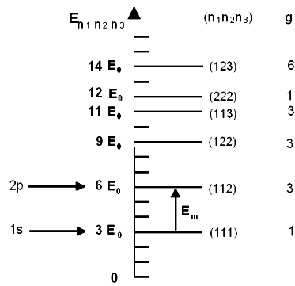
\includegraphics[width=0.8\textwidth]{Figures/Introduction/Quantum.jpg} % Replace 'figure_path' with the actual path to your figure file
    \caption{Energies in the three-dimensional box potential \cite{riede_optical}}
    \label{fig:box_potential}
\end{figure}

\pagebreak{}

\subsubsection{Line Width}

Although one would theoretically expect very narrow absorption bands due to the discrete energy levels, these bands are relatively broad. The reason for this broadening is the interaction of the electron with the surrounding lattice vibrations. To account for this interaction, the configuration coordinate $R$ is introduced, which describes the distance of the surrounding cations from the center of the color center. In the excited states, the electron occupies a larger spatial extent, resulting in $R$ being minimal for the 1s state.

The parabolas representing the energy shift for different values of $R$ and various excited states of the electron, in conjunction with the Franck-Condon principle—which explains the vertical transitions—lead to the observation of relatively broad emission and absorption bands.

\subsubsection{Concentration of Color Centers}

To determine the concentration $N$ of the color centers in the examined lattice, integral absorption is used due to its proportionality. With the approximation by a Lorentz curve and the Drude dispersion theory, the integral absorption is given by:

\begin{equation}
\label{eq:concentration}
\int \alpha \, d\nu = \frac{e^2 N}{4c^2 \epsilon_0 n m_e} \left( \frac{n^2 + 2}{3} \right)^2,
\end{equation}

where $n$ is the refractive index and $m_e$ is the mass of the electron. The absorption coefficient $\alpha$ is obtained via the transmission, i.e., the ratio of the intensities in front of and behind the sample, with:

\begin{equation*}
T = \frac{I_t}{I_0} = \frac{(1 - R) e^{- \alpha d}}{1 - R^2 e^{-2 \alpha d}},
\end{equation*}

where 

\begin{equation*}
R = \frac{(n - 1)^2}{(n + 1)^2}.
\end{equation*}

If $R \ll 1$, Lambert-Beer's law is obtained:

\begin{equation*}
I = I_0 e^{- \alpha d}.
\end{equation*}

\pagebreak{}

\subsection{Experimental Setup}

The Lambda 365 spectrometer used is a dual-beam spectrometer with the following beam path.

\begin{figure}[h]
    \centering
    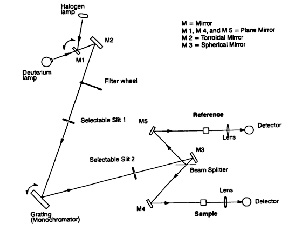
\includegraphics[width=0.8\textwidth]{Figures/Introduction/Path.jpg} % Replace 'figure_path' with the actual path to your figure file
    \caption{Beam path of the spectrometer. From \cite{riede_optical}}
    \label{fig:beam_path}
\end{figure}

The wavelength range of the spectrometer extends from 200 $nm$ to 1100 $nm$. This is achieved using two different lamps, which are switched between at 400 $nm$. A beam splitter divides the light into a measurement beam and a reference beam, allowing for immediate recording of a transmission spectrum without the need for a separate reference measurement. A reflection grating enables precise setting of the wavelength that reaches the sample. By rotating this grating, the entire wavelength range can be covered.

The resolution of the spectrum can be adjusted using two settings: Firstly, the slit width can be adjusted via a selectable slit. Secondly, the speed at which the wavelength range is scanned—known as the registration speed—can be set.

After inserting a sample into the spectrometer, the measurement is initiated electronically, and the transmission spectrum is immediately displayed in the associated software.

\pagebreak{}

\section{Analysis}

\subsection{Task 1}

\textit{By means of absorption bands of a holmium oxide filter determine the wavelength
accuracy of the spectrometer Lambda 365. Investigate the influence of slit width and
scanning speed on the spectrum}

\subsubsection{Optimal Scanning Speed}

To determine the optimal slit width and scanning speed of the lambda 365 spectrometer for our experiment, we first tried to find an optimal scanning speed. This was done by selecting a slit width of 0.5 mm, and varying the scanning speed to find the best one. The results are shown below

\begin{figure}[h]
	\centering
	\scalebox{0.75}{%% Creator: Matplotlib, PGF backend
%%
%% To include the figure in your LaTeX document, write
%%   \input{<filename>.pgf}
%%
%% Make sure the required packages are loaded in your preamble
%%   \usepackage{pgf}
%%
%% Also ensure that all the required font packages are loaded; for instance,
%% the lmodern package is sometimes necessary when using math font.
%%   \usepackage{lmodern}
%%
%% Figures using additional raster images can only be included by \input if
%% they are in the same directory as the main LaTeX file. For loading figures
%% from other directories you can use the `import` package
%%   \usepackage{import}
%%
%% and then include the figures with
%%   \import{<path to file>}{<filename>.pgf}
%%
%% Matplotlib used the following preamble
%%   
%%   \usepackage{fontspec}
%%   \makeatletter\@ifpackageloaded{underscore}{}{\usepackage[strings]{underscore}}\makeatother
%%
\begingroup%
\makeatletter%
\begin{pgfpicture}%
\pgfpathrectangle{\pgfpointorigin}{\pgfqpoint{8.287158in}{5.352321in}}%
\pgfusepath{use as bounding box, clip}%
\begin{pgfscope}%
\pgfsetbuttcap%
\pgfsetmiterjoin%
\definecolor{currentfill}{rgb}{1.000000,1.000000,1.000000}%
\pgfsetfillcolor{currentfill}%
\pgfsetlinewidth{0.000000pt}%
\definecolor{currentstroke}{rgb}{1.000000,1.000000,1.000000}%
\pgfsetstrokecolor{currentstroke}%
\pgfsetdash{}{0pt}%
\pgfpathmoveto{\pgfqpoint{0.000000in}{0.000000in}}%
\pgfpathlineto{\pgfqpoint{8.287158in}{0.000000in}}%
\pgfpathlineto{\pgfqpoint{8.287158in}{5.352321in}}%
\pgfpathlineto{\pgfqpoint{0.000000in}{5.352321in}}%
\pgfpathlineto{\pgfqpoint{0.000000in}{0.000000in}}%
\pgfpathclose%
\pgfusepath{fill}%
\end{pgfscope}%
\begin{pgfscope}%
\pgfsetbuttcap%
\pgfsetmiterjoin%
\definecolor{currentfill}{rgb}{1.000000,1.000000,1.000000}%
\pgfsetfillcolor{currentfill}%
\pgfsetlinewidth{0.000000pt}%
\definecolor{currentstroke}{rgb}{0.000000,0.000000,0.000000}%
\pgfsetstrokecolor{currentstroke}%
\pgfsetstrokeopacity{0.000000}%
\pgfsetdash{}{0pt}%
\pgfpathmoveto{\pgfqpoint{0.643053in}{0.619888in}}%
\pgfpathlineto{\pgfqpoint{8.187158in}{0.619888in}}%
\pgfpathlineto{\pgfqpoint{8.187158in}{5.252321in}}%
\pgfpathlineto{\pgfqpoint{0.643053in}{5.252321in}}%
\pgfpathlineto{\pgfqpoint{0.643053in}{0.619888in}}%
\pgfpathclose%
\pgfusepath{fill}%
\end{pgfscope}%
\begin{pgfscope}%
\pgfpathrectangle{\pgfqpoint{0.643053in}{0.619888in}}{\pgfqpoint{7.544105in}{4.632433in}}%
\pgfusepath{clip}%
\pgfsetbuttcap%
\pgfsetmiterjoin%
\pgfsetlinewidth{1.003750pt}%
\definecolor{currentstroke}{rgb}{0.500000,0.500000,0.500000}%
\pgfsetstrokecolor{currentstroke}%
\pgfsetdash{}{0pt}%
\pgfpathmoveto{\pgfqpoint{2.814841in}{0.863634in}}%
\pgfpathlineto{\pgfqpoint{2.891044in}{0.863634in}}%
\pgfpathlineto{\pgfqpoint{2.891044in}{0.887440in}}%
\pgfpathlineto{\pgfqpoint{2.814841in}{0.887440in}}%
\pgfpathlineto{\pgfqpoint{2.814841in}{0.863634in}}%
\pgfpathclose%
\pgfusepath{stroke}%
\end{pgfscope}%
\begin{pgfscope}%
\pgfsetbuttcap%
\pgfsetroundjoin%
\definecolor{currentfill}{rgb}{0.000000,0.000000,0.000000}%
\pgfsetfillcolor{currentfill}%
\pgfsetlinewidth{0.803000pt}%
\definecolor{currentstroke}{rgb}{0.000000,0.000000,0.000000}%
\pgfsetstrokecolor{currentstroke}%
\pgfsetdash{}{0pt}%
\pgfsys@defobject{currentmarker}{\pgfqpoint{0.000000in}{-0.048611in}}{\pgfqpoint{0.000000in}{0.000000in}}{%
\pgfpathmoveto{\pgfqpoint{0.000000in}{0.000000in}}%
\pgfpathlineto{\pgfqpoint{0.000000in}{-0.048611in}}%
\pgfusepath{stroke,fill}%
}%
\begin{pgfscope}%
\pgfsys@transformshift{0.985967in}{0.619888in}%
\pgfsys@useobject{currentmarker}{}%
\end{pgfscope}%
\end{pgfscope}%
\begin{pgfscope}%
\definecolor{textcolor}{rgb}{0.000000,0.000000,0.000000}%
\pgfsetstrokecolor{textcolor}%
\pgfsetfillcolor{textcolor}%
\pgftext[x=0.985967in,y=0.522666in,,top]{\color{textcolor}\rmfamily\fontsize{14.000000}{16.800000}\selectfont \(\displaystyle {200}\)}%
\end{pgfscope}%
\begin{pgfscope}%
\pgfsetbuttcap%
\pgfsetroundjoin%
\definecolor{currentfill}{rgb}{0.000000,0.000000,0.000000}%
\pgfsetfillcolor{currentfill}%
\pgfsetlinewidth{0.803000pt}%
\definecolor{currentstroke}{rgb}{0.000000,0.000000,0.000000}%
\pgfsetstrokecolor{currentstroke}%
\pgfsetdash{}{0pt}%
\pgfsys@defobject{currentmarker}{\pgfqpoint{0.000000in}{-0.048611in}}{\pgfqpoint{0.000000in}{0.000000in}}{%
\pgfpathmoveto{\pgfqpoint{0.000000in}{0.000000in}}%
\pgfpathlineto{\pgfqpoint{0.000000in}{-0.048611in}}%
\pgfusepath{stroke,fill}%
}%
\begin{pgfscope}%
\pgfsys@transformshift{2.510028in}{0.619888in}%
\pgfsys@useobject{currentmarker}{}%
\end{pgfscope}%
\end{pgfscope}%
\begin{pgfscope}%
\definecolor{textcolor}{rgb}{0.000000,0.000000,0.000000}%
\pgfsetstrokecolor{textcolor}%
\pgfsetfillcolor{textcolor}%
\pgftext[x=2.510028in,y=0.522666in,,top]{\color{textcolor}\rmfamily\fontsize{14.000000}{16.800000}\selectfont \(\displaystyle {400}\)}%
\end{pgfscope}%
\begin{pgfscope}%
\pgfsetbuttcap%
\pgfsetroundjoin%
\definecolor{currentfill}{rgb}{0.000000,0.000000,0.000000}%
\pgfsetfillcolor{currentfill}%
\pgfsetlinewidth{0.803000pt}%
\definecolor{currentstroke}{rgb}{0.000000,0.000000,0.000000}%
\pgfsetstrokecolor{currentstroke}%
\pgfsetdash{}{0pt}%
\pgfsys@defobject{currentmarker}{\pgfqpoint{0.000000in}{-0.048611in}}{\pgfqpoint{0.000000in}{0.000000in}}{%
\pgfpathmoveto{\pgfqpoint{0.000000in}{0.000000in}}%
\pgfpathlineto{\pgfqpoint{0.000000in}{-0.048611in}}%
\pgfusepath{stroke,fill}%
}%
\begin{pgfscope}%
\pgfsys@transformshift{4.034090in}{0.619888in}%
\pgfsys@useobject{currentmarker}{}%
\end{pgfscope}%
\end{pgfscope}%
\begin{pgfscope}%
\definecolor{textcolor}{rgb}{0.000000,0.000000,0.000000}%
\pgfsetstrokecolor{textcolor}%
\pgfsetfillcolor{textcolor}%
\pgftext[x=4.034090in,y=0.522666in,,top]{\color{textcolor}\rmfamily\fontsize{14.000000}{16.800000}\selectfont \(\displaystyle {600}\)}%
\end{pgfscope}%
\begin{pgfscope}%
\pgfsetbuttcap%
\pgfsetroundjoin%
\definecolor{currentfill}{rgb}{0.000000,0.000000,0.000000}%
\pgfsetfillcolor{currentfill}%
\pgfsetlinewidth{0.803000pt}%
\definecolor{currentstroke}{rgb}{0.000000,0.000000,0.000000}%
\pgfsetstrokecolor{currentstroke}%
\pgfsetdash{}{0pt}%
\pgfsys@defobject{currentmarker}{\pgfqpoint{0.000000in}{-0.048611in}}{\pgfqpoint{0.000000in}{0.000000in}}{%
\pgfpathmoveto{\pgfqpoint{0.000000in}{0.000000in}}%
\pgfpathlineto{\pgfqpoint{0.000000in}{-0.048611in}}%
\pgfusepath{stroke,fill}%
}%
\begin{pgfscope}%
\pgfsys@transformshift{5.558152in}{0.619888in}%
\pgfsys@useobject{currentmarker}{}%
\end{pgfscope}%
\end{pgfscope}%
\begin{pgfscope}%
\definecolor{textcolor}{rgb}{0.000000,0.000000,0.000000}%
\pgfsetstrokecolor{textcolor}%
\pgfsetfillcolor{textcolor}%
\pgftext[x=5.558152in,y=0.522666in,,top]{\color{textcolor}\rmfamily\fontsize{14.000000}{16.800000}\selectfont \(\displaystyle {800}\)}%
\end{pgfscope}%
\begin{pgfscope}%
\pgfsetbuttcap%
\pgfsetroundjoin%
\definecolor{currentfill}{rgb}{0.000000,0.000000,0.000000}%
\pgfsetfillcolor{currentfill}%
\pgfsetlinewidth{0.803000pt}%
\definecolor{currentstroke}{rgb}{0.000000,0.000000,0.000000}%
\pgfsetstrokecolor{currentstroke}%
\pgfsetdash{}{0pt}%
\pgfsys@defobject{currentmarker}{\pgfqpoint{0.000000in}{-0.048611in}}{\pgfqpoint{0.000000in}{0.000000in}}{%
\pgfpathmoveto{\pgfqpoint{0.000000in}{0.000000in}}%
\pgfpathlineto{\pgfqpoint{0.000000in}{-0.048611in}}%
\pgfusepath{stroke,fill}%
}%
\begin{pgfscope}%
\pgfsys@transformshift{7.082213in}{0.619888in}%
\pgfsys@useobject{currentmarker}{}%
\end{pgfscope}%
\end{pgfscope}%
\begin{pgfscope}%
\definecolor{textcolor}{rgb}{0.000000,0.000000,0.000000}%
\pgfsetstrokecolor{textcolor}%
\pgfsetfillcolor{textcolor}%
\pgftext[x=7.082213in,y=0.522666in,,top]{\color{textcolor}\rmfamily\fontsize{14.000000}{16.800000}\selectfont \(\displaystyle {1000}\)}%
\end{pgfscope}%
\begin{pgfscope}%
\definecolor{textcolor}{rgb}{0.000000,0.000000,0.000000}%
\pgfsetstrokecolor{textcolor}%
\pgfsetfillcolor{textcolor}%
\pgftext[x=4.415105in,y=0.294444in,,top]{\color{textcolor}\rmfamily\fontsize{14.000000}{16.800000}\selectfont Wavelength [nm]}%
\end{pgfscope}%
\begin{pgfscope}%
\pgfsetbuttcap%
\pgfsetroundjoin%
\definecolor{currentfill}{rgb}{0.000000,0.000000,0.000000}%
\pgfsetfillcolor{currentfill}%
\pgfsetlinewidth{0.803000pt}%
\definecolor{currentstroke}{rgb}{0.000000,0.000000,0.000000}%
\pgfsetstrokecolor{currentstroke}%
\pgfsetdash{}{0pt}%
\pgfsys@defobject{currentmarker}{\pgfqpoint{-0.048611in}{0.000000in}}{\pgfqpoint{-0.000000in}{0.000000in}}{%
\pgfpathmoveto{\pgfqpoint{-0.000000in}{0.000000in}}%
\pgfpathlineto{\pgfqpoint{-0.048611in}{0.000000in}}%
\pgfusepath{stroke,fill}%
}%
\begin{pgfscope}%
\pgfsys@transformshift{0.643053in}{0.830305in}%
\pgfsys@useobject{currentmarker}{}%
\end{pgfscope}%
\end{pgfscope}%
\begin{pgfscope}%
\definecolor{textcolor}{rgb}{0.000000,0.000000,0.000000}%
\pgfsetstrokecolor{textcolor}%
\pgfsetfillcolor{textcolor}%
\pgftext[x=0.447915in, y=0.762833in, left, base]{\color{textcolor}\rmfamily\fontsize{14.000000}{16.800000}\selectfont \(\displaystyle {0}\)}%
\end{pgfscope}%
\begin{pgfscope}%
\pgfsetbuttcap%
\pgfsetroundjoin%
\definecolor{currentfill}{rgb}{0.000000,0.000000,0.000000}%
\pgfsetfillcolor{currentfill}%
\pgfsetlinewidth{0.803000pt}%
\definecolor{currentstroke}{rgb}{0.000000,0.000000,0.000000}%
\pgfsetstrokecolor{currentstroke}%
\pgfsetdash{}{0pt}%
\pgfsys@defobject{currentmarker}{\pgfqpoint{-0.048611in}{0.000000in}}{\pgfqpoint{-0.000000in}{0.000000in}}{%
\pgfpathmoveto{\pgfqpoint{-0.000000in}{0.000000in}}%
\pgfpathlineto{\pgfqpoint{-0.048611in}{0.000000in}}%
\pgfusepath{stroke,fill}%
}%
\begin{pgfscope}%
\pgfsys@transformshift{0.643053in}{1.782558in}%
\pgfsys@useobject{currentmarker}{}%
\end{pgfscope}%
\end{pgfscope}%
\begin{pgfscope}%
\definecolor{textcolor}{rgb}{0.000000,0.000000,0.000000}%
\pgfsetstrokecolor{textcolor}%
\pgfsetfillcolor{textcolor}%
\pgftext[x=0.350000in, y=1.715086in, left, base]{\color{textcolor}\rmfamily\fontsize{14.000000}{16.800000}\selectfont \(\displaystyle {20}\)}%
\end{pgfscope}%
\begin{pgfscope}%
\pgfsetbuttcap%
\pgfsetroundjoin%
\definecolor{currentfill}{rgb}{0.000000,0.000000,0.000000}%
\pgfsetfillcolor{currentfill}%
\pgfsetlinewidth{0.803000pt}%
\definecolor{currentstroke}{rgb}{0.000000,0.000000,0.000000}%
\pgfsetstrokecolor{currentstroke}%
\pgfsetdash{}{0pt}%
\pgfsys@defobject{currentmarker}{\pgfqpoint{-0.048611in}{0.000000in}}{\pgfqpoint{-0.000000in}{0.000000in}}{%
\pgfpathmoveto{\pgfqpoint{-0.000000in}{0.000000in}}%
\pgfpathlineto{\pgfqpoint{-0.048611in}{0.000000in}}%
\pgfusepath{stroke,fill}%
}%
\begin{pgfscope}%
\pgfsys@transformshift{0.643053in}{2.734811in}%
\pgfsys@useobject{currentmarker}{}%
\end{pgfscope}%
\end{pgfscope}%
\begin{pgfscope}%
\definecolor{textcolor}{rgb}{0.000000,0.000000,0.000000}%
\pgfsetstrokecolor{textcolor}%
\pgfsetfillcolor{textcolor}%
\pgftext[x=0.350000in, y=2.667339in, left, base]{\color{textcolor}\rmfamily\fontsize{14.000000}{16.800000}\selectfont \(\displaystyle {40}\)}%
\end{pgfscope}%
\begin{pgfscope}%
\pgfsetbuttcap%
\pgfsetroundjoin%
\definecolor{currentfill}{rgb}{0.000000,0.000000,0.000000}%
\pgfsetfillcolor{currentfill}%
\pgfsetlinewidth{0.803000pt}%
\definecolor{currentstroke}{rgb}{0.000000,0.000000,0.000000}%
\pgfsetstrokecolor{currentstroke}%
\pgfsetdash{}{0pt}%
\pgfsys@defobject{currentmarker}{\pgfqpoint{-0.048611in}{0.000000in}}{\pgfqpoint{-0.000000in}{0.000000in}}{%
\pgfpathmoveto{\pgfqpoint{-0.000000in}{0.000000in}}%
\pgfpathlineto{\pgfqpoint{-0.048611in}{0.000000in}}%
\pgfusepath{stroke,fill}%
}%
\begin{pgfscope}%
\pgfsys@transformshift{0.643053in}{3.687064in}%
\pgfsys@useobject{currentmarker}{}%
\end{pgfscope}%
\end{pgfscope}%
\begin{pgfscope}%
\definecolor{textcolor}{rgb}{0.000000,0.000000,0.000000}%
\pgfsetstrokecolor{textcolor}%
\pgfsetfillcolor{textcolor}%
\pgftext[x=0.350000in, y=3.619592in, left, base]{\color{textcolor}\rmfamily\fontsize{14.000000}{16.800000}\selectfont \(\displaystyle {60}\)}%
\end{pgfscope}%
\begin{pgfscope}%
\pgfsetbuttcap%
\pgfsetroundjoin%
\definecolor{currentfill}{rgb}{0.000000,0.000000,0.000000}%
\pgfsetfillcolor{currentfill}%
\pgfsetlinewidth{0.803000pt}%
\definecolor{currentstroke}{rgb}{0.000000,0.000000,0.000000}%
\pgfsetstrokecolor{currentstroke}%
\pgfsetdash{}{0pt}%
\pgfsys@defobject{currentmarker}{\pgfqpoint{-0.048611in}{0.000000in}}{\pgfqpoint{-0.000000in}{0.000000in}}{%
\pgfpathmoveto{\pgfqpoint{-0.000000in}{0.000000in}}%
\pgfpathlineto{\pgfqpoint{-0.048611in}{0.000000in}}%
\pgfusepath{stroke,fill}%
}%
\begin{pgfscope}%
\pgfsys@transformshift{0.643053in}{4.639317in}%
\pgfsys@useobject{currentmarker}{}%
\end{pgfscope}%
\end{pgfscope}%
\begin{pgfscope}%
\definecolor{textcolor}{rgb}{0.000000,0.000000,0.000000}%
\pgfsetstrokecolor{textcolor}%
\pgfsetfillcolor{textcolor}%
\pgftext[x=0.350000in, y=4.571845in, left, base]{\color{textcolor}\rmfamily\fontsize{14.000000}{16.800000}\selectfont \(\displaystyle {80}\)}%
\end{pgfscope}%
\begin{pgfscope}%
\definecolor{textcolor}{rgb}{0.000000,0.000000,0.000000}%
\pgfsetstrokecolor{textcolor}%
\pgfsetfillcolor{textcolor}%
\pgftext[x=0.294444in,y=2.936105in,,bottom,rotate=90.000000]{\color{textcolor}\rmfamily\fontsize{14.000000}{16.800000}\selectfont Transmittance [\(\displaystyle \%\)]}%
\end{pgfscope}%
\begin{pgfscope}%
\pgfpathrectangle{\pgfqpoint{0.643053in}{0.619888in}}{\pgfqpoint{7.544105in}{4.632433in}}%
\pgfusepath{clip}%
\pgfsetbuttcap%
\pgfsetroundjoin%
\pgfsetlinewidth{1.505625pt}%
\definecolor{currentstroke}{rgb}{0.000000,0.000000,1.000000}%
\pgfsetstrokecolor{currentstroke}%
\pgfsetdash{{5.550000pt}{2.400000pt}}{0.000000pt}%
\pgfpathmoveto{\pgfqpoint{7.844244in}{5.020951in}}%
\pgfpathlineto{\pgfqpoint{7.798522in}{5.027714in}}%
\pgfpathlineto{\pgfqpoint{7.783282in}{5.028476in}}%
\pgfpathlineto{\pgfqpoint{7.768041in}{5.032530in}}%
\pgfpathlineto{\pgfqpoint{7.729940in}{5.033520in}}%
\pgfpathlineto{\pgfqpoint{7.714699in}{5.035768in}}%
\pgfpathlineto{\pgfqpoint{7.691838in}{5.037228in}}%
\pgfpathlineto{\pgfqpoint{7.676598in}{5.037747in}}%
\pgfpathlineto{\pgfqpoint{7.661357in}{5.037308in}}%
\pgfpathlineto{\pgfqpoint{7.653737in}{5.038061in}}%
\pgfpathlineto{\pgfqpoint{7.638496in}{5.037930in}}%
\pgfpathlineto{\pgfqpoint{7.615635in}{5.037641in}}%
\pgfpathlineto{\pgfqpoint{7.608015in}{5.038774in}}%
\pgfpathlineto{\pgfqpoint{7.562293in}{5.038240in}}%
\pgfpathlineto{\pgfqpoint{7.547052in}{5.038639in}}%
\pgfpathlineto{\pgfqpoint{7.539432in}{5.037835in}}%
\pgfpathlineto{\pgfqpoint{7.516571in}{5.039201in}}%
\pgfpathlineto{\pgfqpoint{7.409887in}{5.039285in}}%
\pgfpathlineto{\pgfqpoint{7.173657in}{5.036363in}}%
\pgfpathlineto{\pgfqpoint{7.150796in}{5.036586in}}%
\pgfpathlineto{\pgfqpoint{7.112695in}{5.035810in}}%
\pgfpathlineto{\pgfqpoint{7.051732in}{5.034525in}}%
\pgfpathlineto{\pgfqpoint{6.868845in}{5.029620in}}%
\pgfpathlineto{\pgfqpoint{6.815503in}{5.028652in}}%
\pgfpathlineto{\pgfqpoint{6.602134in}{5.023949in}}%
\pgfpathlineto{\pgfqpoint{6.571653in}{5.021908in}}%
\pgfpathlineto{\pgfqpoint{6.556412in}{5.020566in}}%
\pgfpathlineto{\pgfqpoint{6.541172in}{5.018716in}}%
\pgfpathlineto{\pgfqpoint{6.525931in}{5.014263in}}%
\pgfpathlineto{\pgfqpoint{6.510690in}{5.006572in}}%
\pgfpathlineto{\pgfqpoint{6.480209in}{4.988261in}}%
\pgfpathlineto{\pgfqpoint{6.449728in}{4.974753in}}%
\pgfpathlineto{\pgfqpoint{6.434487in}{4.968793in}}%
\pgfpathlineto{\pgfqpoint{6.426867in}{4.967349in}}%
\pgfpathlineto{\pgfqpoint{6.419247in}{4.967730in}}%
\pgfpathlineto{\pgfqpoint{6.381145in}{4.978212in}}%
\pgfpathlineto{\pgfqpoint{6.350664in}{4.988514in}}%
\pgfpathlineto{\pgfqpoint{6.327803in}{4.992115in}}%
\pgfpathlineto{\pgfqpoint{6.312562in}{4.992097in}}%
\pgfpathlineto{\pgfqpoint{6.297322in}{4.990174in}}%
\pgfpathlineto{\pgfqpoint{6.274461in}{4.982810in}}%
\pgfpathlineto{\pgfqpoint{6.259220in}{4.974136in}}%
\pgfpathlineto{\pgfqpoint{6.236359in}{4.960946in}}%
\pgfpathlineto{\pgfqpoint{6.213498in}{4.951976in}}%
\pgfpathlineto{\pgfqpoint{6.198258in}{4.948845in}}%
\pgfpathlineto{\pgfqpoint{6.183017in}{4.948306in}}%
\pgfpathlineto{\pgfqpoint{6.167776in}{4.955359in}}%
\pgfpathlineto{\pgfqpoint{6.144916in}{4.968554in}}%
\pgfpathlineto{\pgfqpoint{6.129675in}{4.977957in}}%
\pgfpathlineto{\pgfqpoint{6.114434in}{4.986299in}}%
\pgfpathlineto{\pgfqpoint{6.091573in}{4.995377in}}%
\pgfpathlineto{\pgfqpoint{6.076333in}{5.000082in}}%
\pgfpathlineto{\pgfqpoint{6.030611in}{5.004418in}}%
\pgfpathlineto{\pgfqpoint{6.000130in}{5.004981in}}%
\pgfpathlineto{\pgfqpoint{5.939167in}{5.005894in}}%
\pgfpathlineto{\pgfqpoint{5.908686in}{5.004680in}}%
\pgfpathlineto{\pgfqpoint{5.893445in}{5.004528in}}%
\pgfpathlineto{\pgfqpoint{5.878205in}{5.003881in}}%
\pgfpathlineto{\pgfqpoint{5.870584in}{5.004748in}}%
\pgfpathlineto{\pgfqpoint{5.847723in}{5.003178in}}%
\pgfpathlineto{\pgfqpoint{5.756280in}{4.999976in}}%
\pgfpathlineto{\pgfqpoint{5.741039in}{5.000343in}}%
\pgfpathlineto{\pgfqpoint{5.718178in}{4.998491in}}%
\pgfpathlineto{\pgfqpoint{5.702938in}{4.999067in}}%
\pgfpathlineto{\pgfqpoint{5.687697in}{4.997477in}}%
\pgfpathlineto{\pgfqpoint{5.672456in}{4.997286in}}%
\pgfpathlineto{\pgfqpoint{5.641975in}{4.994662in}}%
\pgfpathlineto{\pgfqpoint{5.619114in}{4.994186in}}%
\pgfpathlineto{\pgfqpoint{5.603874in}{4.993260in}}%
\pgfpathlineto{\pgfqpoint{5.596253in}{4.993514in}}%
\pgfpathlineto{\pgfqpoint{5.573392in}{4.991360in}}%
\pgfpathlineto{\pgfqpoint{5.558152in}{4.992716in}}%
\pgfpathlineto{\pgfqpoint{5.550531in}{4.991110in}}%
\pgfpathlineto{\pgfqpoint{5.527671in}{4.990109in}}%
\pgfpathlineto{\pgfqpoint{5.520050in}{4.990991in}}%
\pgfpathlineto{\pgfqpoint{5.497189in}{4.989094in}}%
\pgfpathlineto{\pgfqpoint{5.436227in}{4.987791in}}%
\pgfpathlineto{\pgfqpoint{5.428607in}{4.987869in}}%
\pgfpathlineto{\pgfqpoint{5.413366in}{4.985186in}}%
\pgfpathlineto{\pgfqpoint{5.398125in}{4.984950in}}%
\pgfpathlineto{\pgfqpoint{5.382885in}{4.982586in}}%
\pgfpathlineto{\pgfqpoint{5.352403in}{4.980307in}}%
\pgfpathlineto{\pgfqpoint{5.260960in}{4.978019in}}%
\pgfpathlineto{\pgfqpoint{5.207618in}{4.972264in}}%
\pgfpathlineto{\pgfqpoint{5.123794in}{4.971721in}}%
\pgfpathlineto{\pgfqpoint{5.108554in}{4.970860in}}%
\pgfpathlineto{\pgfqpoint{5.093313in}{4.969654in}}%
\pgfpathlineto{\pgfqpoint{5.078072in}{4.968880in}}%
\pgfpathlineto{\pgfqpoint{5.062832in}{4.968684in}}%
\pgfpathlineto{\pgfqpoint{5.039971in}{4.970129in}}%
\pgfpathlineto{\pgfqpoint{4.933286in}{4.967001in}}%
\pgfpathlineto{\pgfqpoint{4.910426in}{4.965843in}}%
\pgfpathlineto{\pgfqpoint{4.826602in}{4.962384in}}%
\pgfpathlineto{\pgfqpoint{4.811362in}{4.961702in}}%
\pgfpathlineto{\pgfqpoint{4.697057in}{4.955113in}}%
\pgfpathlineto{\pgfqpoint{4.689437in}{4.954124in}}%
\pgfpathlineto{\pgfqpoint{4.674196in}{4.954157in}}%
\pgfpathlineto{\pgfqpoint{4.658955in}{4.952677in}}%
\pgfpathlineto{\pgfqpoint{4.620854in}{4.944654in}}%
\pgfpathlineto{\pgfqpoint{4.605613in}{4.938381in}}%
\pgfpathlineto{\pgfqpoint{4.597993in}{4.932903in}}%
\pgfpathlineto{\pgfqpoint{4.590373in}{4.925328in}}%
\pgfpathlineto{\pgfqpoint{4.582752in}{4.914760in}}%
\pgfpathlineto{\pgfqpoint{4.575132in}{4.897097in}}%
\pgfpathlineto{\pgfqpoint{4.567512in}{4.863463in}}%
\pgfpathlineto{\pgfqpoint{4.559891in}{4.813344in}}%
\pgfpathlineto{\pgfqpoint{4.529410in}{4.570204in}}%
\pgfpathlineto{\pgfqpoint{4.521790in}{4.525002in}}%
\pgfpathlineto{\pgfqpoint{4.514170in}{4.495101in}}%
\pgfpathlineto{\pgfqpoint{4.506549in}{4.486756in}}%
\pgfpathlineto{\pgfqpoint{4.498929in}{4.502478in}}%
\pgfpathlineto{\pgfqpoint{4.476068in}{4.565353in}}%
\pgfpathlineto{\pgfqpoint{4.468448in}{4.581790in}}%
\pgfpathlineto{\pgfqpoint{4.460827in}{4.581459in}}%
\pgfpathlineto{\pgfqpoint{4.453207in}{4.554491in}}%
\pgfpathlineto{\pgfqpoint{4.445587in}{4.505744in}}%
\pgfpathlineto{\pgfqpoint{4.437966in}{4.439445in}}%
\pgfpathlineto{\pgfqpoint{4.422726in}{4.274621in}}%
\pgfpathlineto{\pgfqpoint{4.415105in}{4.190897in}}%
\pgfpathlineto{\pgfqpoint{4.407485in}{4.161642in}}%
\pgfpathlineto{\pgfqpoint{4.399865in}{4.170596in}}%
\pgfpathlineto{\pgfqpoint{4.392245in}{4.192170in}}%
\pgfpathlineto{\pgfqpoint{4.377004in}{4.208734in}}%
\pgfpathlineto{\pgfqpoint{4.369384in}{4.209655in}}%
\pgfpathlineto{\pgfqpoint{4.361763in}{4.189427in}}%
\pgfpathlineto{\pgfqpoint{4.354143in}{4.139460in}}%
\pgfpathlineto{\pgfqpoint{4.346523in}{4.056904in}}%
\pgfpathlineto{\pgfqpoint{4.338902in}{3.953147in}}%
\pgfpathlineto{\pgfqpoint{4.331282in}{3.879086in}}%
\pgfpathlineto{\pgfqpoint{4.323662in}{3.846808in}}%
\pgfpathlineto{\pgfqpoint{4.316041in}{3.855954in}}%
\pgfpathlineto{\pgfqpoint{4.308421in}{3.901336in}}%
\pgfpathlineto{\pgfqpoint{4.300801in}{3.978225in}}%
\pgfpathlineto{\pgfqpoint{4.293181in}{4.102570in}}%
\pgfpathlineto{\pgfqpoint{4.270320in}{4.547694in}}%
\pgfpathlineto{\pgfqpoint{4.262699in}{4.648320in}}%
\pgfpathlineto{\pgfqpoint{4.255079in}{4.713909in}}%
\pgfpathlineto{\pgfqpoint{4.247459in}{4.759527in}}%
\pgfpathlineto{\pgfqpoint{4.239838in}{4.792457in}}%
\pgfpathlineto{\pgfqpoint{4.232218in}{4.817583in}}%
\pgfpathlineto{\pgfqpoint{4.224598in}{4.836890in}}%
\pgfpathlineto{\pgfqpoint{4.209357in}{4.863174in}}%
\pgfpathlineto{\pgfqpoint{4.201737in}{4.873567in}}%
\pgfpathlineto{\pgfqpoint{4.186496in}{4.888641in}}%
\pgfpathlineto{\pgfqpoint{4.171256in}{4.900399in}}%
\pgfpathlineto{\pgfqpoint{4.156015in}{4.909062in}}%
\pgfpathlineto{\pgfqpoint{4.148395in}{4.912205in}}%
\pgfpathlineto{\pgfqpoint{4.133154in}{4.914927in}}%
\pgfpathlineto{\pgfqpoint{4.064571in}{4.916257in}}%
\pgfpathlineto{\pgfqpoint{4.049331in}{4.914517in}}%
\pgfpathlineto{\pgfqpoint{4.026470in}{4.912701in}}%
\pgfpathlineto{\pgfqpoint{4.018849in}{4.911499in}}%
\pgfpathlineto{\pgfqpoint{3.935026in}{4.912818in}}%
\pgfpathlineto{\pgfqpoint{3.912165in}{4.911897in}}%
\pgfpathlineto{\pgfqpoint{3.874064in}{4.911101in}}%
\pgfpathlineto{\pgfqpoint{3.866443in}{4.909696in}}%
\pgfpathlineto{\pgfqpoint{3.828342in}{4.908635in}}%
\pgfpathlineto{\pgfqpoint{3.813101in}{4.906307in}}%
\pgfpathlineto{\pgfqpoint{3.782620in}{4.903777in}}%
\pgfpathlineto{\pgfqpoint{3.744518in}{4.897570in}}%
\pgfpathlineto{\pgfqpoint{3.729278in}{4.890634in}}%
\pgfpathlineto{\pgfqpoint{3.721657in}{4.886008in}}%
\pgfpathlineto{\pgfqpoint{3.714037in}{4.878953in}}%
\pgfpathlineto{\pgfqpoint{3.706417in}{4.864350in}}%
\pgfpathlineto{\pgfqpoint{3.698796in}{4.833195in}}%
\pgfpathlineto{\pgfqpoint{3.691176in}{4.775264in}}%
\pgfpathlineto{\pgfqpoint{3.675936in}{4.633203in}}%
\pgfpathlineto{\pgfqpoint{3.668315in}{4.591111in}}%
\pgfpathlineto{\pgfqpoint{3.660695in}{4.533671in}}%
\pgfpathlineto{\pgfqpoint{3.653075in}{4.459095in}}%
\pgfpathlineto{\pgfqpoint{3.645454in}{4.355842in}}%
\pgfpathlineto{\pgfqpoint{3.637834in}{4.230046in}}%
\pgfpathlineto{\pgfqpoint{3.630214in}{4.154724in}}%
\pgfpathlineto{\pgfqpoint{3.622593in}{4.144133in}}%
\pgfpathlineto{\pgfqpoint{3.614973in}{4.148266in}}%
\pgfpathlineto{\pgfqpoint{3.607353in}{4.139026in}}%
\pgfpathlineto{\pgfqpoint{3.599732in}{4.085937in}}%
\pgfpathlineto{\pgfqpoint{3.592112in}{3.950420in}}%
\pgfpathlineto{\pgfqpoint{3.584492in}{3.766648in}}%
\pgfpathlineto{\pgfqpoint{3.561631in}{2.957149in}}%
\pgfpathlineto{\pgfqpoint{3.554011in}{2.836497in}}%
\pgfpathlineto{\pgfqpoint{3.546390in}{2.863260in}}%
\pgfpathlineto{\pgfqpoint{3.538770in}{3.100970in}}%
\pgfpathlineto{\pgfqpoint{3.515909in}{4.217594in}}%
\pgfpathlineto{\pgfqpoint{3.508289in}{4.425941in}}%
\pgfpathlineto{\pgfqpoint{3.500668in}{4.558827in}}%
\pgfpathlineto{\pgfqpoint{3.493048in}{4.645915in}}%
\pgfpathlineto{\pgfqpoint{3.485428in}{4.703465in}}%
\pgfpathlineto{\pgfqpoint{3.477808in}{4.743224in}}%
\pgfpathlineto{\pgfqpoint{3.470187in}{4.771599in}}%
\pgfpathlineto{\pgfqpoint{3.462567in}{4.792814in}}%
\pgfpathlineto{\pgfqpoint{3.454947in}{4.808729in}}%
\pgfpathlineto{\pgfqpoint{3.447326in}{4.819708in}}%
\pgfpathlineto{\pgfqpoint{3.432086in}{4.832450in}}%
\pgfpathlineto{\pgfqpoint{3.416845in}{4.840887in}}%
\pgfpathlineto{\pgfqpoint{3.401604in}{4.847615in}}%
\pgfpathlineto{\pgfqpoint{3.393984in}{4.855150in}}%
\pgfpathlineto{\pgfqpoint{3.386364in}{4.856600in}}%
\pgfpathlineto{\pgfqpoint{3.378744in}{4.855594in}}%
\pgfpathlineto{\pgfqpoint{3.348262in}{4.847098in}}%
\pgfpathlineto{\pgfqpoint{3.333022in}{4.844343in}}%
\pgfpathlineto{\pgfqpoint{3.325401in}{4.844772in}}%
\pgfpathlineto{\pgfqpoint{3.317781in}{4.847747in}}%
\pgfpathlineto{\pgfqpoint{3.294920in}{4.849912in}}%
\pgfpathlineto{\pgfqpoint{3.279680in}{4.846720in}}%
\pgfpathlineto{\pgfqpoint{3.272059in}{4.842582in}}%
\pgfpathlineto{\pgfqpoint{3.264439in}{4.835915in}}%
\pgfpathlineto{\pgfqpoint{3.256819in}{4.825718in}}%
\pgfpathlineto{\pgfqpoint{3.249198in}{4.808482in}}%
\pgfpathlineto{\pgfqpoint{3.241578in}{4.779759in}}%
\pgfpathlineto{\pgfqpoint{3.233958in}{4.738296in}}%
\pgfpathlineto{\pgfqpoint{3.226337in}{4.689420in}}%
\pgfpathlineto{\pgfqpoint{3.218717in}{4.614770in}}%
\pgfpathlineto{\pgfqpoint{3.188236in}{4.250829in}}%
\pgfpathlineto{\pgfqpoint{3.180616in}{4.213263in}}%
\pgfpathlineto{\pgfqpoint{3.165375in}{4.225704in}}%
\pgfpathlineto{\pgfqpoint{3.157755in}{4.164636in}}%
\pgfpathlineto{\pgfqpoint{3.150134in}{4.168187in}}%
\pgfpathlineto{\pgfqpoint{3.142514in}{4.257898in}}%
\pgfpathlineto{\pgfqpoint{3.134894in}{4.376579in}}%
\pgfpathlineto{\pgfqpoint{3.119653in}{4.570678in}}%
\pgfpathlineto{\pgfqpoint{3.112033in}{4.606093in}}%
\pgfpathlineto{\pgfqpoint{3.104412in}{4.553812in}}%
\pgfpathlineto{\pgfqpoint{3.096792in}{4.433246in}}%
\pgfpathlineto{\pgfqpoint{3.089172in}{4.284906in}}%
\pgfpathlineto{\pgfqpoint{3.081552in}{4.174298in}}%
\pgfpathlineto{\pgfqpoint{3.073931in}{4.135678in}}%
\pgfpathlineto{\pgfqpoint{3.066311in}{4.155872in}}%
\pgfpathlineto{\pgfqpoint{3.051070in}{4.240289in}}%
\pgfpathlineto{\pgfqpoint{3.043450in}{4.294578in}}%
\pgfpathlineto{\pgfqpoint{3.035830in}{4.231469in}}%
\pgfpathlineto{\pgfqpoint{3.028209in}{4.076897in}}%
\pgfpathlineto{\pgfqpoint{3.020589in}{3.889159in}}%
\pgfpathlineto{\pgfqpoint{3.012969in}{3.632055in}}%
\pgfpathlineto{\pgfqpoint{3.005348in}{3.172472in}}%
\pgfpathlineto{\pgfqpoint{2.997728in}{2.466236in}}%
\pgfpathlineto{\pgfqpoint{2.990108in}{1.988808in}}%
\pgfpathlineto{\pgfqpoint{2.982487in}{1.639112in}}%
\pgfpathlineto{\pgfqpoint{2.974867in}{1.362100in}}%
\pgfpathlineto{\pgfqpoint{2.967247in}{1.204064in}}%
\pgfpathlineto{\pgfqpoint{2.959627in}{1.376648in}}%
\pgfpathlineto{\pgfqpoint{2.952006in}{1.807930in}}%
\pgfpathlineto{\pgfqpoint{2.944386in}{2.136743in}}%
\pgfpathlineto{\pgfqpoint{2.936766in}{2.085701in}}%
\pgfpathlineto{\pgfqpoint{2.929145in}{1.703294in}}%
\pgfpathlineto{\pgfqpoint{2.921525in}{1.415003in}}%
\pgfpathlineto{\pgfqpoint{2.913905in}{1.364219in}}%
\pgfpathlineto{\pgfqpoint{2.906284in}{1.532465in}}%
\pgfpathlineto{\pgfqpoint{2.898664in}{1.819138in}}%
\pgfpathlineto{\pgfqpoint{2.891044in}{1.936867in}}%
\pgfpathlineto{\pgfqpoint{2.875803in}{1.121189in}}%
\pgfpathlineto{\pgfqpoint{2.868183in}{0.918176in}}%
\pgfpathlineto{\pgfqpoint{2.860563in}{0.868537in}}%
\pgfpathlineto{\pgfqpoint{2.852942in}{0.868847in}}%
\pgfpathlineto{\pgfqpoint{2.845322in}{1.103348in}}%
\pgfpathlineto{\pgfqpoint{2.830081in}{3.083814in}}%
\pgfpathlineto{\pgfqpoint{2.822461in}{3.727654in}}%
\pgfpathlineto{\pgfqpoint{2.814841in}{4.048843in}}%
\pgfpathlineto{\pgfqpoint{2.807220in}{4.236022in}}%
\pgfpathlineto{\pgfqpoint{2.799600in}{4.378826in}}%
\pgfpathlineto{\pgfqpoint{2.791980in}{4.485640in}}%
\pgfpathlineto{\pgfqpoint{2.784359in}{4.556639in}}%
\pgfpathlineto{\pgfqpoint{2.776739in}{4.594958in}}%
\pgfpathlineto{\pgfqpoint{2.769119in}{4.609454in}}%
\pgfpathlineto{\pgfqpoint{2.761499in}{4.616240in}}%
\pgfpathlineto{\pgfqpoint{2.753878in}{4.630505in}}%
\pgfpathlineto{\pgfqpoint{2.746258in}{4.639855in}}%
\pgfpathlineto{\pgfqpoint{2.738638in}{4.630343in}}%
\pgfpathlineto{\pgfqpoint{2.731017in}{4.589680in}}%
\pgfpathlineto{\pgfqpoint{2.723397in}{4.515729in}}%
\pgfpathlineto{\pgfqpoint{2.708156in}{4.265979in}}%
\pgfpathlineto{\pgfqpoint{2.700536in}{4.201860in}}%
\pgfpathlineto{\pgfqpoint{2.692916in}{4.233559in}}%
\pgfpathlineto{\pgfqpoint{2.685295in}{4.353245in}}%
\pgfpathlineto{\pgfqpoint{2.677675in}{4.242131in}}%
\pgfpathlineto{\pgfqpoint{2.670055in}{3.968094in}}%
\pgfpathlineto{\pgfqpoint{2.662435in}{3.647132in}}%
\pgfpathlineto{\pgfqpoint{2.654814in}{3.428000in}}%
\pgfpathlineto{\pgfqpoint{2.647194in}{3.467410in}}%
\pgfpathlineto{\pgfqpoint{2.639574in}{3.856919in}}%
\pgfpathlineto{\pgfqpoint{2.631953in}{4.062525in}}%
\pgfpathlineto{\pgfqpoint{2.624333in}{4.149430in}}%
\pgfpathlineto{\pgfqpoint{2.616713in}{4.213584in}}%
\pgfpathlineto{\pgfqpoint{2.609092in}{4.344989in}}%
\pgfpathlineto{\pgfqpoint{2.601472in}{4.496131in}}%
\pgfpathlineto{\pgfqpoint{2.593852in}{4.581516in}}%
\pgfpathlineto{\pgfqpoint{2.586231in}{4.632911in}}%
\pgfpathlineto{\pgfqpoint{2.578611in}{4.662643in}}%
\pgfpathlineto{\pgfqpoint{2.570991in}{4.678556in}}%
\pgfpathlineto{\pgfqpoint{2.555750in}{4.688069in}}%
\pgfpathlineto{\pgfqpoint{2.548130in}{4.689398in}}%
\pgfpathlineto{\pgfqpoint{2.532889in}{4.684450in}}%
\pgfpathlineto{\pgfqpoint{2.525269in}{4.686745in}}%
\pgfpathlineto{\pgfqpoint{2.517649in}{4.683193in}}%
\pgfpathlineto{\pgfqpoint{2.510028in}{4.675015in}}%
\pgfpathlineto{\pgfqpoint{2.502408in}{4.649791in}}%
\pgfpathlineto{\pgfqpoint{2.494788in}{4.658130in}}%
\pgfpathlineto{\pgfqpoint{2.487167in}{4.654397in}}%
\pgfpathlineto{\pgfqpoint{2.479547in}{4.635632in}}%
\pgfpathlineto{\pgfqpoint{2.471927in}{4.636534in}}%
\pgfpathlineto{\pgfqpoint{2.464307in}{4.626498in}}%
\pgfpathlineto{\pgfqpoint{2.456686in}{4.591026in}}%
\pgfpathlineto{\pgfqpoint{2.449066in}{4.532137in}}%
\pgfpathlineto{\pgfqpoint{2.441446in}{4.513365in}}%
\pgfpathlineto{\pgfqpoint{2.433825in}{4.538245in}}%
\pgfpathlineto{\pgfqpoint{2.426205in}{4.530606in}}%
\pgfpathlineto{\pgfqpoint{2.418585in}{4.454038in}}%
\pgfpathlineto{\pgfqpoint{2.410964in}{4.304508in}}%
\pgfpathlineto{\pgfqpoint{2.403344in}{4.230076in}}%
\pgfpathlineto{\pgfqpoint{2.395724in}{4.338699in}}%
\pgfpathlineto{\pgfqpoint{2.388103in}{4.430663in}}%
\pgfpathlineto{\pgfqpoint{2.380483in}{4.406156in}}%
\pgfpathlineto{\pgfqpoint{2.372863in}{4.246667in}}%
\pgfpathlineto{\pgfqpoint{2.357622in}{4.511511in}}%
\pgfpathlineto{\pgfqpoint{2.350002in}{4.571019in}}%
\pgfpathlineto{\pgfqpoint{2.342382in}{4.565020in}}%
\pgfpathlineto{\pgfqpoint{2.334761in}{4.573115in}}%
\pgfpathlineto{\pgfqpoint{2.311900in}{4.579251in}}%
\pgfpathlineto{\pgfqpoint{2.304280in}{4.572839in}}%
\pgfpathlineto{\pgfqpoint{2.296660in}{4.543442in}}%
\pgfpathlineto{\pgfqpoint{2.273799in}{4.153863in}}%
\pgfpathlineto{\pgfqpoint{2.266178in}{4.080201in}}%
\pgfpathlineto{\pgfqpoint{2.258558in}{4.041305in}}%
\pgfpathlineto{\pgfqpoint{2.250938in}{3.809951in}}%
\pgfpathlineto{\pgfqpoint{2.235697in}{3.166663in}}%
\pgfpathlineto{\pgfqpoint{2.228077in}{2.766568in}}%
\pgfpathlineto{\pgfqpoint{2.220457in}{2.160593in}}%
\pgfpathlineto{\pgfqpoint{2.212836in}{1.340672in}}%
\pgfpathlineto{\pgfqpoint{2.205216in}{2.107144in}}%
\pgfpathlineto{\pgfqpoint{2.197596in}{3.068566in}}%
\pgfpathlineto{\pgfqpoint{2.189975in}{3.749947in}}%
\pgfpathlineto{\pgfqpoint{2.182355in}{4.127364in}}%
\pgfpathlineto{\pgfqpoint{2.174735in}{4.257910in}}%
\pgfpathlineto{\pgfqpoint{2.167114in}{4.317717in}}%
\pgfpathlineto{\pgfqpoint{2.159494in}{4.331398in}}%
\pgfpathlineto{\pgfqpoint{2.151874in}{4.317285in}}%
\pgfpathlineto{\pgfqpoint{2.144254in}{4.292973in}}%
\pgfpathlineto{\pgfqpoint{2.136633in}{4.303635in}}%
\pgfpathlineto{\pgfqpoint{2.129013in}{4.256601in}}%
\pgfpathlineto{\pgfqpoint{2.121393in}{4.171993in}}%
\pgfpathlineto{\pgfqpoint{2.113772in}{4.110491in}}%
\pgfpathlineto{\pgfqpoint{2.106152in}{4.137288in}}%
\pgfpathlineto{\pgfqpoint{2.098532in}{4.201909in}}%
\pgfpathlineto{\pgfqpoint{2.090911in}{4.167569in}}%
\pgfpathlineto{\pgfqpoint{2.083291in}{4.189220in}}%
\pgfpathlineto{\pgfqpoint{2.075671in}{4.240756in}}%
\pgfpathlineto{\pgfqpoint{2.068050in}{4.255931in}}%
\pgfpathlineto{\pgfqpoint{2.060430in}{4.251520in}}%
\pgfpathlineto{\pgfqpoint{2.052810in}{4.269604in}}%
\pgfpathlineto{\pgfqpoint{2.045190in}{4.274958in}}%
\pgfpathlineto{\pgfqpoint{2.037569in}{4.251658in}}%
\pgfpathlineto{\pgfqpoint{2.029949in}{4.201532in}}%
\pgfpathlineto{\pgfqpoint{2.022329in}{4.163021in}}%
\pgfpathlineto{\pgfqpoint{2.007088in}{3.827694in}}%
\pgfpathlineto{\pgfqpoint{1.999468in}{3.886444in}}%
\pgfpathlineto{\pgfqpoint{1.991847in}{4.152755in}}%
\pgfpathlineto{\pgfqpoint{1.976607in}{4.300450in}}%
\pgfpathlineto{\pgfqpoint{1.968986in}{4.319308in}}%
\pgfpathlineto{\pgfqpoint{1.961366in}{4.315347in}}%
\pgfpathlineto{\pgfqpoint{1.953746in}{4.306108in}}%
\pgfpathlineto{\pgfqpoint{1.946126in}{4.287852in}}%
\pgfpathlineto{\pgfqpoint{1.938505in}{4.283250in}}%
\pgfpathlineto{\pgfqpoint{1.923265in}{4.239645in}}%
\pgfpathlineto{\pgfqpoint{1.915644in}{4.229727in}}%
\pgfpathlineto{\pgfqpoint{1.908024in}{4.227694in}}%
\pgfpathlineto{\pgfqpoint{1.892783in}{4.205547in}}%
\pgfpathlineto{\pgfqpoint{1.877543in}{4.179087in}}%
\pgfpathlineto{\pgfqpoint{1.862302in}{4.145323in}}%
\pgfpathlineto{\pgfqpoint{1.854682in}{4.134706in}}%
\pgfpathlineto{\pgfqpoint{1.839441in}{4.103271in}}%
\pgfpathlineto{\pgfqpoint{1.831821in}{4.094388in}}%
\pgfpathlineto{\pgfqpoint{1.824201in}{4.076534in}}%
\pgfpathlineto{\pgfqpoint{1.808960in}{4.047569in}}%
\pgfpathlineto{\pgfqpoint{1.793719in}{4.012570in}}%
\pgfpathlineto{\pgfqpoint{1.778479in}{3.975700in}}%
\pgfpathlineto{\pgfqpoint{1.755618in}{3.903431in}}%
\pgfpathlineto{\pgfqpoint{1.747998in}{3.868912in}}%
\pgfpathlineto{\pgfqpoint{1.740377in}{3.822392in}}%
\pgfpathlineto{\pgfqpoint{1.725137in}{3.706122in}}%
\pgfpathlineto{\pgfqpoint{1.702276in}{3.492024in}}%
\pgfpathlineto{\pgfqpoint{1.694655in}{3.452398in}}%
\pgfpathlineto{\pgfqpoint{1.687035in}{3.356891in}}%
\pgfpathlineto{\pgfqpoint{1.679415in}{3.149911in}}%
\pgfpathlineto{\pgfqpoint{1.671794in}{2.892150in}}%
\pgfpathlineto{\pgfqpoint{1.664174in}{3.018392in}}%
\pgfpathlineto{\pgfqpoint{1.656554in}{2.473479in}}%
\pgfpathlineto{\pgfqpoint{1.648934in}{2.793875in}}%
\pgfpathlineto{\pgfqpoint{1.641313in}{3.302805in}}%
\pgfpathlineto{\pgfqpoint{1.633693in}{3.427166in}}%
\pgfpathlineto{\pgfqpoint{1.626073in}{3.409606in}}%
\pgfpathlineto{\pgfqpoint{1.618452in}{3.347940in}}%
\pgfpathlineto{\pgfqpoint{1.610832in}{3.240896in}}%
\pgfpathlineto{\pgfqpoint{1.603212in}{2.971573in}}%
\pgfpathlineto{\pgfqpoint{1.595591in}{2.533066in}}%
\pgfpathlineto{\pgfqpoint{1.587971in}{2.384194in}}%
\pgfpathlineto{\pgfqpoint{1.580351in}{2.801266in}}%
\pgfpathlineto{\pgfqpoint{1.572730in}{3.001115in}}%
\pgfpathlineto{\pgfqpoint{1.565110in}{3.016883in}}%
\pgfpathlineto{\pgfqpoint{1.557490in}{3.005725in}}%
\pgfpathlineto{\pgfqpoint{1.542249in}{3.010684in}}%
\pgfpathlineto{\pgfqpoint{1.534629in}{2.995124in}}%
\pgfpathlineto{\pgfqpoint{1.519388in}{2.935183in}}%
\pgfpathlineto{\pgfqpoint{1.511768in}{2.918503in}}%
\pgfpathlineto{\pgfqpoint{1.496527in}{2.840253in}}%
\pgfpathlineto{\pgfqpoint{1.488907in}{2.785827in}}%
\pgfpathlineto{\pgfqpoint{1.473666in}{2.647949in}}%
\pgfpathlineto{\pgfqpoint{1.466046in}{2.496242in}}%
\pgfpathlineto{\pgfqpoint{1.450805in}{2.440424in}}%
\pgfpathlineto{\pgfqpoint{1.443185in}{2.425141in}}%
\pgfpathlineto{\pgfqpoint{1.435565in}{2.456573in}}%
\pgfpathlineto{\pgfqpoint{1.427945in}{2.423581in}}%
\pgfpathlineto{\pgfqpoint{1.420324in}{2.374098in}}%
\pgfpathlineto{\pgfqpoint{1.405084in}{2.251774in}}%
\pgfpathlineto{\pgfqpoint{1.397463in}{2.184800in}}%
\pgfpathlineto{\pgfqpoint{1.389843in}{2.101055in}}%
\pgfpathlineto{\pgfqpoint{1.374602in}{1.874911in}}%
\pgfpathlineto{\pgfqpoint{1.366982in}{1.797501in}}%
\pgfpathlineto{\pgfqpoint{1.359362in}{1.737688in}}%
\pgfpathlineto{\pgfqpoint{1.351741in}{1.657554in}}%
\pgfpathlineto{\pgfqpoint{1.336501in}{1.440444in}}%
\pgfpathlineto{\pgfqpoint{1.313640in}{1.070303in}}%
\pgfpathlineto{\pgfqpoint{1.306020in}{0.937877in}}%
\pgfpathlineto{\pgfqpoint{1.298399in}{0.909812in}}%
\pgfpathlineto{\pgfqpoint{1.290779in}{0.895739in}}%
\pgfpathlineto{\pgfqpoint{1.283159in}{0.863626in}}%
\pgfpathlineto{\pgfqpoint{1.275538in}{0.840279in}}%
\pgfpathlineto{\pgfqpoint{1.267918in}{0.832210in}}%
\pgfpathlineto{\pgfqpoint{1.260298in}{0.830456in}}%
\pgfpathlineto{\pgfqpoint{0.985967in}{0.830742in}}%
\pgfpathlineto{\pgfqpoint{0.985967in}{0.830742in}}%
\pgfusepath{stroke}%
\end{pgfscope}%
\begin{pgfscope}%
\pgfpathrectangle{\pgfqpoint{0.643053in}{0.619888in}}{\pgfqpoint{7.544105in}{4.632433in}}%
\pgfusepath{clip}%
\pgfsetbuttcap%
\pgfsetroundjoin%
\pgfsetlinewidth{1.505625pt}%
\definecolor{currentstroke}{rgb}{1.000000,0.000000,0.000000}%
\pgfsetstrokecolor{currentstroke}%
\pgfsetdash{{9.600000pt}{2.400000pt}{1.500000pt}{2.400000pt}}{0.000000pt}%
\pgfpathmoveto{\pgfqpoint{7.844244in}{5.021490in}}%
\pgfpathlineto{\pgfqpoint{7.813763in}{5.025647in}}%
\pgfpathlineto{\pgfqpoint{7.806143in}{5.024944in}}%
\pgfpathlineto{\pgfqpoint{7.798522in}{5.027785in}}%
\pgfpathlineto{\pgfqpoint{7.783282in}{5.029931in}}%
\pgfpathlineto{\pgfqpoint{7.729940in}{5.032523in}}%
\pgfpathlineto{\pgfqpoint{7.722319in}{5.034655in}}%
\pgfpathlineto{\pgfqpoint{7.707079in}{5.034442in}}%
\pgfpathlineto{\pgfqpoint{7.691838in}{5.033990in}}%
\pgfpathlineto{\pgfqpoint{7.676598in}{5.034987in}}%
\pgfpathlineto{\pgfqpoint{7.661357in}{5.035922in}}%
\pgfpathlineto{\pgfqpoint{7.638496in}{5.035705in}}%
\pgfpathlineto{\pgfqpoint{7.623255in}{5.038406in}}%
\pgfpathlineto{\pgfqpoint{7.585154in}{5.037537in}}%
\pgfpathlineto{\pgfqpoint{7.577534in}{5.036758in}}%
\pgfpathlineto{\pgfqpoint{7.569913in}{5.038252in}}%
\pgfpathlineto{\pgfqpoint{7.554673in}{5.036939in}}%
\pgfpathlineto{\pgfqpoint{7.508951in}{5.036820in}}%
\pgfpathlineto{\pgfqpoint{7.493710in}{5.036424in}}%
\pgfpathlineto{\pgfqpoint{7.478470in}{5.035865in}}%
\pgfpathlineto{\pgfqpoint{7.447988in}{5.036455in}}%
\pgfpathlineto{\pgfqpoint{7.417507in}{5.035173in}}%
\pgfpathlineto{\pgfqpoint{7.402266in}{5.035511in}}%
\pgfpathlineto{\pgfqpoint{7.364165in}{5.033662in}}%
\pgfpathlineto{\pgfqpoint{7.341304in}{5.032564in}}%
\pgfpathlineto{\pgfqpoint{7.326063in}{5.031933in}}%
\pgfpathlineto{\pgfqpoint{7.280342in}{5.031366in}}%
\pgfpathlineto{\pgfqpoint{7.257481in}{5.030097in}}%
\pgfpathlineto{\pgfqpoint{7.234620in}{5.030511in}}%
\pgfpathlineto{\pgfqpoint{7.211759in}{5.029877in}}%
\pgfpathlineto{\pgfqpoint{7.150796in}{5.029179in}}%
\pgfpathlineto{\pgfqpoint{7.135556in}{5.028849in}}%
\pgfpathlineto{\pgfqpoint{7.006010in}{5.027273in}}%
\pgfpathlineto{\pgfqpoint{6.983149in}{5.026576in}}%
\pgfpathlineto{\pgfqpoint{6.937428in}{5.026020in}}%
\pgfpathlineto{\pgfqpoint{6.655476in}{5.020744in}}%
\pgfpathlineto{\pgfqpoint{6.647856in}{5.019327in}}%
\pgfpathlineto{\pgfqpoint{6.632615in}{5.019616in}}%
\pgfpathlineto{\pgfqpoint{6.564033in}{5.015303in}}%
\pgfpathlineto{\pgfqpoint{6.541172in}{5.012656in}}%
\pgfpathlineto{\pgfqpoint{6.533551in}{5.010769in}}%
\pgfpathlineto{\pgfqpoint{6.518311in}{5.004067in}}%
\pgfpathlineto{\pgfqpoint{6.472589in}{4.977782in}}%
\pgfpathlineto{\pgfqpoint{6.442108in}{4.964864in}}%
\pgfpathlineto{\pgfqpoint{6.434487in}{4.961893in}}%
\pgfpathlineto{\pgfqpoint{6.426867in}{4.960266in}}%
\pgfpathlineto{\pgfqpoint{6.419247in}{4.960706in}}%
\pgfpathlineto{\pgfqpoint{6.396386in}{4.966844in}}%
\pgfpathlineto{\pgfqpoint{6.343044in}{4.983162in}}%
\pgfpathlineto{\pgfqpoint{6.335423in}{4.984768in}}%
\pgfpathlineto{\pgfqpoint{6.312562in}{4.985306in}}%
\pgfpathlineto{\pgfqpoint{6.304942in}{4.984914in}}%
\pgfpathlineto{\pgfqpoint{6.274461in}{4.974829in}}%
\pgfpathlineto{\pgfqpoint{6.259220in}{4.968060in}}%
\pgfpathlineto{\pgfqpoint{6.243980in}{4.958207in}}%
\pgfpathlineto{\pgfqpoint{6.228739in}{4.950598in}}%
\pgfpathlineto{\pgfqpoint{6.213498in}{4.945330in}}%
\pgfpathlineto{\pgfqpoint{6.198258in}{4.943000in}}%
\pgfpathlineto{\pgfqpoint{6.183017in}{4.942402in}}%
\pgfpathlineto{\pgfqpoint{6.167776in}{4.948336in}}%
\pgfpathlineto{\pgfqpoint{6.122055in}{4.976167in}}%
\pgfpathlineto{\pgfqpoint{6.099194in}{4.986614in}}%
\pgfpathlineto{\pgfqpoint{6.076333in}{4.992931in}}%
\pgfpathlineto{\pgfqpoint{6.053472in}{4.996052in}}%
\pgfpathlineto{\pgfqpoint{6.038231in}{4.997201in}}%
\pgfpathlineto{\pgfqpoint{6.030611in}{4.996972in}}%
\pgfpathlineto{\pgfqpoint{6.022991in}{4.998155in}}%
\pgfpathlineto{\pgfqpoint{6.007750in}{4.997673in}}%
\pgfpathlineto{\pgfqpoint{5.962028in}{4.999116in}}%
\pgfpathlineto{\pgfqpoint{5.923927in}{4.996928in}}%
\pgfpathlineto{\pgfqpoint{5.908686in}{4.997797in}}%
\pgfpathlineto{\pgfqpoint{5.885825in}{4.996876in}}%
\pgfpathlineto{\pgfqpoint{5.832483in}{4.994233in}}%
\pgfpathlineto{\pgfqpoint{5.824863in}{4.994903in}}%
\pgfpathlineto{\pgfqpoint{5.809622in}{4.994241in}}%
\pgfpathlineto{\pgfqpoint{5.802002in}{4.994482in}}%
\pgfpathlineto{\pgfqpoint{5.794381in}{4.993353in}}%
\pgfpathlineto{\pgfqpoint{5.786761in}{4.993967in}}%
\pgfpathlineto{\pgfqpoint{5.771520in}{4.992186in}}%
\pgfpathlineto{\pgfqpoint{5.748659in}{4.992176in}}%
\pgfpathlineto{\pgfqpoint{5.588633in}{4.986744in}}%
\pgfpathlineto{\pgfqpoint{5.558152in}{4.985699in}}%
\pgfpathlineto{\pgfqpoint{5.542911in}{4.985085in}}%
\pgfpathlineto{\pgfqpoint{5.512430in}{4.983382in}}%
\pgfpathlineto{\pgfqpoint{5.504810in}{4.982606in}}%
\pgfpathlineto{\pgfqpoint{5.489569in}{4.984049in}}%
\pgfpathlineto{\pgfqpoint{5.466708in}{4.981658in}}%
\pgfpathlineto{\pgfqpoint{5.398125in}{4.977748in}}%
\pgfpathlineto{\pgfqpoint{5.360024in}{4.973346in}}%
\pgfpathlineto{\pgfqpoint{5.344783in}{4.973454in}}%
\pgfpathlineto{\pgfqpoint{5.337163in}{4.973785in}}%
\pgfpathlineto{\pgfqpoint{5.321922in}{4.972639in}}%
\pgfpathlineto{\pgfqpoint{5.276200in}{4.970803in}}%
\pgfpathlineto{\pgfqpoint{5.260960in}{4.969980in}}%
\pgfpathlineto{\pgfqpoint{5.245719in}{4.969273in}}%
\pgfpathlineto{\pgfqpoint{5.222858in}{4.966685in}}%
\pgfpathlineto{\pgfqpoint{5.192377in}{4.964603in}}%
\pgfpathlineto{\pgfqpoint{5.154275in}{4.963822in}}%
\pgfpathlineto{\pgfqpoint{5.131414in}{4.963815in}}%
\pgfpathlineto{\pgfqpoint{5.070452in}{4.961394in}}%
\pgfpathlineto{\pgfqpoint{5.024730in}{4.961470in}}%
\pgfpathlineto{\pgfqpoint{5.001869in}{4.961172in}}%
\pgfpathlineto{\pgfqpoint{4.864704in}{4.955322in}}%
\pgfpathlineto{\pgfqpoint{4.849463in}{4.955225in}}%
\pgfpathlineto{\pgfqpoint{4.826602in}{4.953538in}}%
\pgfpathlineto{\pgfqpoint{4.811362in}{4.952936in}}%
\pgfpathlineto{\pgfqpoint{4.788501in}{4.951401in}}%
\pgfpathlineto{\pgfqpoint{4.666576in}{4.943971in}}%
\pgfpathlineto{\pgfqpoint{4.628474in}{4.938100in}}%
\pgfpathlineto{\pgfqpoint{4.620854in}{4.936360in}}%
\pgfpathlineto{\pgfqpoint{4.605613in}{4.929674in}}%
\pgfpathlineto{\pgfqpoint{4.597993in}{4.924707in}}%
\pgfpathlineto{\pgfqpoint{4.590373in}{4.917469in}}%
\pgfpathlineto{\pgfqpoint{4.582752in}{4.906493in}}%
\pgfpathlineto{\pgfqpoint{4.575132in}{4.888355in}}%
\pgfpathlineto{\pgfqpoint{4.567512in}{4.854574in}}%
\pgfpathlineto{\pgfqpoint{4.559891in}{4.805508in}}%
\pgfpathlineto{\pgfqpoint{4.529410in}{4.562151in}}%
\pgfpathlineto{\pgfqpoint{4.521790in}{4.516749in}}%
\pgfpathlineto{\pgfqpoint{4.514170in}{4.486657in}}%
\pgfpathlineto{\pgfqpoint{4.506549in}{4.478783in}}%
\pgfpathlineto{\pgfqpoint{4.498929in}{4.495086in}}%
\pgfpathlineto{\pgfqpoint{4.468448in}{4.573735in}}%
\pgfpathlineto{\pgfqpoint{4.460827in}{4.572897in}}%
\pgfpathlineto{\pgfqpoint{4.453207in}{4.545962in}}%
\pgfpathlineto{\pgfqpoint{4.445587in}{4.497191in}}%
\pgfpathlineto{\pgfqpoint{4.437966in}{4.430766in}}%
\pgfpathlineto{\pgfqpoint{4.415105in}{4.182812in}}%
\pgfpathlineto{\pgfqpoint{4.407485in}{4.154717in}}%
\pgfpathlineto{\pgfqpoint{4.399865in}{4.163997in}}%
\pgfpathlineto{\pgfqpoint{4.392245in}{4.185483in}}%
\pgfpathlineto{\pgfqpoint{4.377004in}{4.201648in}}%
\pgfpathlineto{\pgfqpoint{4.369384in}{4.202540in}}%
\pgfpathlineto{\pgfqpoint{4.361763in}{4.182401in}}%
\pgfpathlineto{\pgfqpoint{4.354143in}{4.132044in}}%
\pgfpathlineto{\pgfqpoint{4.346523in}{4.048654in}}%
\pgfpathlineto{\pgfqpoint{4.338902in}{3.947058in}}%
\pgfpathlineto{\pgfqpoint{4.331282in}{3.872270in}}%
\pgfpathlineto{\pgfqpoint{4.323662in}{3.840504in}}%
\pgfpathlineto{\pgfqpoint{4.316041in}{3.850797in}}%
\pgfpathlineto{\pgfqpoint{4.308421in}{3.896772in}}%
\pgfpathlineto{\pgfqpoint{4.300801in}{3.973431in}}%
\pgfpathlineto{\pgfqpoint{4.293181in}{4.098438in}}%
\pgfpathlineto{\pgfqpoint{4.270320in}{4.539306in}}%
\pgfpathlineto{\pgfqpoint{4.262699in}{4.640002in}}%
\pgfpathlineto{\pgfqpoint{4.255079in}{4.705061in}}%
\pgfpathlineto{\pgfqpoint{4.247459in}{4.751536in}}%
\pgfpathlineto{\pgfqpoint{4.239838in}{4.784850in}}%
\pgfpathlineto{\pgfqpoint{4.232218in}{4.809195in}}%
\pgfpathlineto{\pgfqpoint{4.224598in}{4.827429in}}%
\pgfpathlineto{\pgfqpoint{4.216977in}{4.842367in}}%
\pgfpathlineto{\pgfqpoint{4.201737in}{4.863522in}}%
\pgfpathlineto{\pgfqpoint{4.186496in}{4.880671in}}%
\pgfpathlineto{\pgfqpoint{4.163635in}{4.897210in}}%
\pgfpathlineto{\pgfqpoint{4.148395in}{4.902786in}}%
\pgfpathlineto{\pgfqpoint{4.133154in}{4.905214in}}%
\pgfpathlineto{\pgfqpoint{4.110293in}{4.906409in}}%
\pgfpathlineto{\pgfqpoint{4.079812in}{4.907159in}}%
\pgfpathlineto{\pgfqpoint{4.064571in}{4.906984in}}%
\pgfpathlineto{\pgfqpoint{4.026470in}{4.901798in}}%
\pgfpathlineto{\pgfqpoint{4.018849in}{4.902814in}}%
\pgfpathlineto{\pgfqpoint{4.003609in}{4.902058in}}%
\pgfpathlineto{\pgfqpoint{3.957887in}{4.904060in}}%
\pgfpathlineto{\pgfqpoint{3.904545in}{4.902101in}}%
\pgfpathlineto{\pgfqpoint{3.835962in}{4.898309in}}%
\pgfpathlineto{\pgfqpoint{3.820721in}{4.896825in}}%
\pgfpathlineto{\pgfqpoint{3.767379in}{4.892125in}}%
\pgfpathlineto{\pgfqpoint{3.759759in}{4.890961in}}%
\pgfpathlineto{\pgfqpoint{3.729278in}{4.881191in}}%
\pgfpathlineto{\pgfqpoint{3.721657in}{4.876004in}}%
\pgfpathlineto{\pgfqpoint{3.714037in}{4.868497in}}%
\pgfpathlineto{\pgfqpoint{3.706417in}{4.854760in}}%
\pgfpathlineto{\pgfqpoint{3.698796in}{4.823683in}}%
\pgfpathlineto{\pgfqpoint{3.691176in}{4.765527in}}%
\pgfpathlineto{\pgfqpoint{3.675936in}{4.624474in}}%
\pgfpathlineto{\pgfqpoint{3.668315in}{4.581428in}}%
\pgfpathlineto{\pgfqpoint{3.660695in}{4.523951in}}%
\pgfpathlineto{\pgfqpoint{3.653075in}{4.448100in}}%
\pgfpathlineto{\pgfqpoint{3.645454in}{4.343922in}}%
\pgfpathlineto{\pgfqpoint{3.637834in}{4.219085in}}%
\pgfpathlineto{\pgfqpoint{3.630214in}{4.146289in}}%
\pgfpathlineto{\pgfqpoint{3.622593in}{4.134926in}}%
\pgfpathlineto{\pgfqpoint{3.614973in}{4.139299in}}%
\pgfpathlineto{\pgfqpoint{3.607353in}{4.129729in}}%
\pgfpathlineto{\pgfqpoint{3.599732in}{4.075661in}}%
\pgfpathlineto{\pgfqpoint{3.592112in}{3.942010in}}%
\pgfpathlineto{\pgfqpoint{3.584492in}{3.758487in}}%
\pgfpathlineto{\pgfqpoint{3.561631in}{2.952330in}}%
\pgfpathlineto{\pgfqpoint{3.554011in}{2.831918in}}%
\pgfpathlineto{\pgfqpoint{3.546390in}{2.858462in}}%
\pgfpathlineto{\pgfqpoint{3.538770in}{3.098070in}}%
\pgfpathlineto{\pgfqpoint{3.515909in}{4.213438in}}%
\pgfpathlineto{\pgfqpoint{3.508289in}{4.420102in}}%
\pgfpathlineto{\pgfqpoint{3.500668in}{4.550471in}}%
\pgfpathlineto{\pgfqpoint{3.493048in}{4.636356in}}%
\pgfpathlineto{\pgfqpoint{3.485428in}{4.693435in}}%
\pgfpathlineto{\pgfqpoint{3.477808in}{4.731887in}}%
\pgfpathlineto{\pgfqpoint{3.470187in}{4.759964in}}%
\pgfpathlineto{\pgfqpoint{3.462567in}{4.781082in}}%
\pgfpathlineto{\pgfqpoint{3.454947in}{4.796885in}}%
\pgfpathlineto{\pgfqpoint{3.447326in}{4.808664in}}%
\pgfpathlineto{\pgfqpoint{3.439706in}{4.817412in}}%
\pgfpathlineto{\pgfqpoint{3.416845in}{4.829743in}}%
\pgfpathlineto{\pgfqpoint{3.409225in}{4.832565in}}%
\pgfpathlineto{\pgfqpoint{3.393984in}{4.841444in}}%
\pgfpathlineto{\pgfqpoint{3.386364in}{4.843620in}}%
\pgfpathlineto{\pgfqpoint{3.378744in}{4.844305in}}%
\pgfpathlineto{\pgfqpoint{3.371123in}{4.842874in}}%
\pgfpathlineto{\pgfqpoint{3.348262in}{4.834225in}}%
\pgfpathlineto{\pgfqpoint{3.340642in}{4.833124in}}%
\pgfpathlineto{\pgfqpoint{3.317781in}{4.834531in}}%
\pgfpathlineto{\pgfqpoint{3.302540in}{4.837458in}}%
\pgfpathlineto{\pgfqpoint{3.294920in}{4.837189in}}%
\pgfpathlineto{\pgfqpoint{3.279680in}{4.834491in}}%
\pgfpathlineto{\pgfqpoint{3.272059in}{4.830800in}}%
\pgfpathlineto{\pgfqpoint{3.264439in}{4.824143in}}%
\pgfpathlineto{\pgfqpoint{3.256819in}{4.813305in}}%
\pgfpathlineto{\pgfqpoint{3.249198in}{4.795826in}}%
\pgfpathlineto{\pgfqpoint{3.241578in}{4.768443in}}%
\pgfpathlineto{\pgfqpoint{3.226337in}{4.677298in}}%
\pgfpathlineto{\pgfqpoint{3.218717in}{4.602854in}}%
\pgfpathlineto{\pgfqpoint{3.188236in}{4.239739in}}%
\pgfpathlineto{\pgfqpoint{3.180616in}{4.204500in}}%
\pgfpathlineto{\pgfqpoint{3.172995in}{4.211272in}}%
\pgfpathlineto{\pgfqpoint{3.165375in}{4.215905in}}%
\pgfpathlineto{\pgfqpoint{3.157755in}{4.155413in}}%
\pgfpathlineto{\pgfqpoint{3.150134in}{4.157274in}}%
\pgfpathlineto{\pgfqpoint{3.142514in}{4.247068in}}%
\pgfpathlineto{\pgfqpoint{3.134894in}{4.365014in}}%
\pgfpathlineto{\pgfqpoint{3.119653in}{4.557955in}}%
\pgfpathlineto{\pgfqpoint{3.112033in}{4.594180in}}%
\pgfpathlineto{\pgfqpoint{3.104412in}{4.542522in}}%
\pgfpathlineto{\pgfqpoint{3.096792in}{4.422377in}}%
\pgfpathlineto{\pgfqpoint{3.089172in}{4.274070in}}%
\pgfpathlineto{\pgfqpoint{3.081552in}{4.162491in}}%
\pgfpathlineto{\pgfqpoint{3.073931in}{4.124161in}}%
\pgfpathlineto{\pgfqpoint{3.066311in}{4.144671in}}%
\pgfpathlineto{\pgfqpoint{3.051070in}{4.229822in}}%
\pgfpathlineto{\pgfqpoint{3.043450in}{4.284384in}}%
\pgfpathlineto{\pgfqpoint{3.035830in}{4.220245in}}%
\pgfpathlineto{\pgfqpoint{3.028209in}{4.064561in}}%
\pgfpathlineto{\pgfqpoint{3.020589in}{3.878055in}}%
\pgfpathlineto{\pgfqpoint{3.012969in}{3.624792in}}%
\pgfpathlineto{\pgfqpoint{3.005348in}{3.168434in}}%
\pgfpathlineto{\pgfqpoint{2.997728in}{2.461657in}}%
\pgfpathlineto{\pgfqpoint{2.990108in}{1.985912in}}%
\pgfpathlineto{\pgfqpoint{2.982487in}{1.636155in}}%
\pgfpathlineto{\pgfqpoint{2.974867in}{1.357783in}}%
\pgfpathlineto{\pgfqpoint{2.967247in}{1.204704in}}%
\pgfpathlineto{\pgfqpoint{2.959627in}{1.381522in}}%
\pgfpathlineto{\pgfqpoint{2.952006in}{1.811903in}}%
\pgfpathlineto{\pgfqpoint{2.944386in}{2.135048in}}%
\pgfpathlineto{\pgfqpoint{2.936766in}{2.076937in}}%
\pgfpathlineto{\pgfqpoint{2.929145in}{1.695339in}}%
\pgfpathlineto{\pgfqpoint{2.921525in}{1.412408in}}%
\pgfpathlineto{\pgfqpoint{2.913905in}{1.365923in}}%
\pgfpathlineto{\pgfqpoint{2.906284in}{1.533158in}}%
\pgfpathlineto{\pgfqpoint{2.898664in}{1.813045in}}%
\pgfpathlineto{\pgfqpoint{2.891044in}{1.936647in}}%
\pgfpathlineto{\pgfqpoint{2.875803in}{1.125430in}}%
\pgfpathlineto{\pgfqpoint{2.868183in}{0.921258in}}%
\pgfpathlineto{\pgfqpoint{2.860563in}{0.871707in}}%
\pgfpathlineto{\pgfqpoint{2.852942in}{0.872114in}}%
\pgfpathlineto{\pgfqpoint{2.845322in}{1.111912in}}%
\pgfpathlineto{\pgfqpoint{2.830081in}{3.088765in}}%
\pgfpathlineto{\pgfqpoint{2.822461in}{3.719760in}}%
\pgfpathlineto{\pgfqpoint{2.814841in}{4.040086in}}%
\pgfpathlineto{\pgfqpoint{2.807220in}{4.227147in}}%
\pgfpathlineto{\pgfqpoint{2.799600in}{4.366365in}}%
\pgfpathlineto{\pgfqpoint{2.791980in}{4.471366in}}%
\pgfpathlineto{\pgfqpoint{2.784359in}{4.542644in}}%
\pgfpathlineto{\pgfqpoint{2.776739in}{4.581904in}}%
\pgfpathlineto{\pgfqpoint{2.769119in}{4.595560in}}%
\pgfpathlineto{\pgfqpoint{2.761499in}{4.604284in}}%
\pgfpathlineto{\pgfqpoint{2.753878in}{4.618560in}}%
\pgfpathlineto{\pgfqpoint{2.746258in}{4.627432in}}%
\pgfpathlineto{\pgfqpoint{2.738638in}{4.616887in}}%
\pgfpathlineto{\pgfqpoint{2.731017in}{4.573831in}}%
\pgfpathlineto{\pgfqpoint{2.723397in}{4.500739in}}%
\pgfpathlineto{\pgfqpoint{2.708156in}{4.252984in}}%
\pgfpathlineto{\pgfqpoint{2.700536in}{4.189793in}}%
\pgfpathlineto{\pgfqpoint{2.692916in}{4.218435in}}%
\pgfpathlineto{\pgfqpoint{2.685295in}{4.336968in}}%
\pgfpathlineto{\pgfqpoint{2.677675in}{4.227732in}}%
\pgfpathlineto{\pgfqpoint{2.670055in}{3.956628in}}%
\pgfpathlineto{\pgfqpoint{2.662435in}{3.637213in}}%
\pgfpathlineto{\pgfqpoint{2.654814in}{3.418078in}}%
\pgfpathlineto{\pgfqpoint{2.647194in}{3.456341in}}%
\pgfpathlineto{\pgfqpoint{2.639574in}{3.843857in}}%
\pgfpathlineto{\pgfqpoint{2.631953in}{4.046248in}}%
\pgfpathlineto{\pgfqpoint{2.624333in}{4.134028in}}%
\pgfpathlineto{\pgfqpoint{2.616713in}{4.201248in}}%
\pgfpathlineto{\pgfqpoint{2.601472in}{4.479989in}}%
\pgfpathlineto{\pgfqpoint{2.593852in}{4.566432in}}%
\pgfpathlineto{\pgfqpoint{2.586231in}{4.616395in}}%
\pgfpathlineto{\pgfqpoint{2.578611in}{4.642469in}}%
\pgfpathlineto{\pgfqpoint{2.570991in}{4.655780in}}%
\pgfpathlineto{\pgfqpoint{2.563371in}{4.664956in}}%
\pgfpathlineto{\pgfqpoint{2.555750in}{4.668279in}}%
\pgfpathlineto{\pgfqpoint{2.548130in}{4.669539in}}%
\pgfpathlineto{\pgfqpoint{2.540510in}{4.668878in}}%
\pgfpathlineto{\pgfqpoint{2.525269in}{4.663324in}}%
\pgfpathlineto{\pgfqpoint{2.517649in}{4.664410in}}%
\pgfpathlineto{\pgfqpoint{2.510028in}{4.659814in}}%
\pgfpathlineto{\pgfqpoint{2.502408in}{4.633844in}}%
\pgfpathlineto{\pgfqpoint{2.494788in}{4.630902in}}%
\pgfpathlineto{\pgfqpoint{2.487167in}{4.651297in}}%
\pgfpathlineto{\pgfqpoint{2.479547in}{4.627973in}}%
\pgfpathlineto{\pgfqpoint{2.471927in}{4.625304in}}%
\pgfpathlineto{\pgfqpoint{2.464307in}{4.618864in}}%
\pgfpathlineto{\pgfqpoint{2.456686in}{4.593505in}}%
\pgfpathlineto{\pgfqpoint{2.449066in}{4.546269in}}%
\pgfpathlineto{\pgfqpoint{2.441446in}{4.506394in}}%
\pgfpathlineto{\pgfqpoint{2.433825in}{4.520900in}}%
\pgfpathlineto{\pgfqpoint{2.426205in}{4.512243in}}%
\pgfpathlineto{\pgfqpoint{2.418585in}{4.439049in}}%
\pgfpathlineto{\pgfqpoint{2.410964in}{4.291848in}}%
\pgfpathlineto{\pgfqpoint{2.403344in}{4.217456in}}%
\pgfpathlineto{\pgfqpoint{2.388103in}{4.400670in}}%
\pgfpathlineto{\pgfqpoint{2.380483in}{4.391873in}}%
\pgfpathlineto{\pgfqpoint{2.372863in}{4.227958in}}%
\pgfpathlineto{\pgfqpoint{2.357622in}{4.493574in}}%
\pgfpathlineto{\pgfqpoint{2.350002in}{4.553109in}}%
\pgfpathlineto{\pgfqpoint{2.342382in}{4.560834in}}%
\pgfpathlineto{\pgfqpoint{2.334761in}{4.559924in}}%
\pgfpathlineto{\pgfqpoint{2.319521in}{4.586676in}}%
\pgfpathlineto{\pgfqpoint{2.311900in}{4.590376in}}%
\pgfpathlineto{\pgfqpoint{2.304280in}{4.577786in}}%
\pgfpathlineto{\pgfqpoint{2.296660in}{4.547139in}}%
\pgfpathlineto{\pgfqpoint{2.289039in}{4.422415in}}%
\pgfpathlineto{\pgfqpoint{2.281419in}{4.271073in}}%
\pgfpathlineto{\pgfqpoint{2.273799in}{4.154851in}}%
\pgfpathlineto{\pgfqpoint{2.266178in}{4.086370in}}%
\pgfpathlineto{\pgfqpoint{2.258558in}{4.035911in}}%
\pgfpathlineto{\pgfqpoint{2.250938in}{3.800442in}}%
\pgfpathlineto{\pgfqpoint{2.235697in}{3.174548in}}%
\pgfpathlineto{\pgfqpoint{2.228077in}{2.776945in}}%
\pgfpathlineto{\pgfqpoint{2.220457in}{2.174448in}}%
\pgfpathlineto{\pgfqpoint{2.212836in}{1.367303in}}%
\pgfpathlineto{\pgfqpoint{2.205216in}{2.118023in}}%
\pgfpathlineto{\pgfqpoint{2.197596in}{3.074346in}}%
\pgfpathlineto{\pgfqpoint{2.189975in}{3.761775in}}%
\pgfpathlineto{\pgfqpoint{2.182355in}{4.118169in}}%
\pgfpathlineto{\pgfqpoint{2.174735in}{4.252028in}}%
\pgfpathlineto{\pgfqpoint{2.167114in}{4.300158in}}%
\pgfpathlineto{\pgfqpoint{2.159494in}{4.313926in}}%
\pgfpathlineto{\pgfqpoint{2.151874in}{4.309692in}}%
\pgfpathlineto{\pgfqpoint{2.144254in}{4.287250in}}%
\pgfpathlineto{\pgfqpoint{2.136633in}{4.303294in}}%
\pgfpathlineto{\pgfqpoint{2.129013in}{4.262180in}}%
\pgfpathlineto{\pgfqpoint{2.121393in}{4.177286in}}%
\pgfpathlineto{\pgfqpoint{2.113772in}{4.112822in}}%
\pgfpathlineto{\pgfqpoint{2.106152in}{4.139548in}}%
\pgfpathlineto{\pgfqpoint{2.098532in}{4.195625in}}%
\pgfpathlineto{\pgfqpoint{2.090911in}{4.172647in}}%
\pgfpathlineto{\pgfqpoint{2.083291in}{4.190370in}}%
\pgfpathlineto{\pgfqpoint{2.075671in}{4.234765in}}%
\pgfpathlineto{\pgfqpoint{2.068050in}{4.258593in}}%
\pgfpathlineto{\pgfqpoint{2.060430in}{4.256091in}}%
\pgfpathlineto{\pgfqpoint{2.052810in}{4.272023in}}%
\pgfpathlineto{\pgfqpoint{2.045190in}{4.258922in}}%
\pgfpathlineto{\pgfqpoint{2.029949in}{4.199991in}}%
\pgfpathlineto{\pgfqpoint{2.022329in}{4.147519in}}%
\pgfpathlineto{\pgfqpoint{2.007088in}{3.831487in}}%
\pgfpathlineto{\pgfqpoint{1.999468in}{3.888444in}}%
\pgfpathlineto{\pgfqpoint{1.991847in}{4.141233in}}%
\pgfpathlineto{\pgfqpoint{1.976607in}{4.281937in}}%
\pgfpathlineto{\pgfqpoint{1.968986in}{4.311924in}}%
\pgfpathlineto{\pgfqpoint{1.961366in}{4.317454in}}%
\pgfpathlineto{\pgfqpoint{1.953746in}{4.309687in}}%
\pgfpathlineto{\pgfqpoint{1.946126in}{4.291068in}}%
\pgfpathlineto{\pgfqpoint{1.930885in}{4.246200in}}%
\pgfpathlineto{\pgfqpoint{1.923265in}{4.229399in}}%
\pgfpathlineto{\pgfqpoint{1.915644in}{4.219413in}}%
\pgfpathlineto{\pgfqpoint{1.908024in}{4.214683in}}%
\pgfpathlineto{\pgfqpoint{1.900404in}{4.207634in}}%
\pgfpathlineto{\pgfqpoint{1.892783in}{4.195410in}}%
\pgfpathlineto{\pgfqpoint{1.885163in}{4.177188in}}%
\pgfpathlineto{\pgfqpoint{1.877543in}{4.162561in}}%
\pgfpathlineto{\pgfqpoint{1.869922in}{4.157791in}}%
\pgfpathlineto{\pgfqpoint{1.847062in}{4.108007in}}%
\pgfpathlineto{\pgfqpoint{1.839441in}{4.093937in}}%
\pgfpathlineto{\pgfqpoint{1.831821in}{4.083392in}}%
\pgfpathlineto{\pgfqpoint{1.816580in}{4.047573in}}%
\pgfpathlineto{\pgfqpoint{1.808960in}{4.035104in}}%
\pgfpathlineto{\pgfqpoint{1.801340in}{4.019943in}}%
\pgfpathlineto{\pgfqpoint{1.778479in}{3.962209in}}%
\pgfpathlineto{\pgfqpoint{1.770858in}{3.944734in}}%
\pgfpathlineto{\pgfqpoint{1.763238in}{3.923835in}}%
\pgfpathlineto{\pgfqpoint{1.755618in}{3.897259in}}%
\pgfpathlineto{\pgfqpoint{1.747998in}{3.864569in}}%
\pgfpathlineto{\pgfqpoint{1.740377in}{3.818490in}}%
\pgfpathlineto{\pgfqpoint{1.725137in}{3.698356in}}%
\pgfpathlineto{\pgfqpoint{1.702276in}{3.489864in}}%
\pgfpathlineto{\pgfqpoint{1.694655in}{3.449940in}}%
\pgfpathlineto{\pgfqpoint{1.687035in}{3.342757in}}%
\pgfpathlineto{\pgfqpoint{1.679415in}{3.133507in}}%
\pgfpathlineto{\pgfqpoint{1.671794in}{2.891888in}}%
\pgfpathlineto{\pgfqpoint{1.664174in}{3.006083in}}%
\pgfpathlineto{\pgfqpoint{1.656554in}{2.464136in}}%
\pgfpathlineto{\pgfqpoint{1.648934in}{2.788275in}}%
\pgfpathlineto{\pgfqpoint{1.641313in}{3.298108in}}%
\pgfpathlineto{\pgfqpoint{1.633693in}{3.418951in}}%
\pgfpathlineto{\pgfqpoint{1.626073in}{3.402897in}}%
\pgfpathlineto{\pgfqpoint{1.618452in}{3.344216in}}%
\pgfpathlineto{\pgfqpoint{1.610832in}{3.232244in}}%
\pgfpathlineto{\pgfqpoint{1.603212in}{2.956182in}}%
\pgfpathlineto{\pgfqpoint{1.595591in}{2.517513in}}%
\pgfpathlineto{\pgfqpoint{1.587971in}{2.393971in}}%
\pgfpathlineto{\pgfqpoint{1.580351in}{2.803699in}}%
\pgfpathlineto{\pgfqpoint{1.572730in}{2.999522in}}%
\pgfpathlineto{\pgfqpoint{1.565110in}{3.013806in}}%
\pgfpathlineto{\pgfqpoint{1.557490in}{2.999698in}}%
\pgfpathlineto{\pgfqpoint{1.549869in}{3.003271in}}%
\pgfpathlineto{\pgfqpoint{1.542249in}{3.005169in}}%
\pgfpathlineto{\pgfqpoint{1.534629in}{2.990739in}}%
\pgfpathlineto{\pgfqpoint{1.519388in}{2.925969in}}%
\pgfpathlineto{\pgfqpoint{1.511768in}{2.913468in}}%
\pgfpathlineto{\pgfqpoint{1.496527in}{2.829169in}}%
\pgfpathlineto{\pgfqpoint{1.488907in}{2.773735in}}%
\pgfpathlineto{\pgfqpoint{1.473666in}{2.638720in}}%
\pgfpathlineto{\pgfqpoint{1.466046in}{2.487721in}}%
\pgfpathlineto{\pgfqpoint{1.450805in}{2.432294in}}%
\pgfpathlineto{\pgfqpoint{1.443185in}{2.416427in}}%
\pgfpathlineto{\pgfqpoint{1.435565in}{2.447900in}}%
\pgfpathlineto{\pgfqpoint{1.427945in}{2.415362in}}%
\pgfpathlineto{\pgfqpoint{1.420324in}{2.365570in}}%
\pgfpathlineto{\pgfqpoint{1.405084in}{2.243973in}}%
\pgfpathlineto{\pgfqpoint{1.397463in}{2.175275in}}%
\pgfpathlineto{\pgfqpoint{1.389843in}{2.093913in}}%
\pgfpathlineto{\pgfqpoint{1.374602in}{1.867220in}}%
\pgfpathlineto{\pgfqpoint{1.366982in}{1.789185in}}%
\pgfpathlineto{\pgfqpoint{1.359362in}{1.728182in}}%
\pgfpathlineto{\pgfqpoint{1.351741in}{1.650926in}}%
\pgfpathlineto{\pgfqpoint{1.336501in}{1.434476in}}%
\pgfpathlineto{\pgfqpoint{1.313640in}{1.066425in}}%
\pgfpathlineto{\pgfqpoint{1.306020in}{0.938199in}}%
\pgfpathlineto{\pgfqpoint{1.298399in}{0.910220in}}%
\pgfpathlineto{\pgfqpoint{1.290779in}{0.894990in}}%
\pgfpathlineto{\pgfqpoint{1.283159in}{0.862419in}}%
\pgfpathlineto{\pgfqpoint{1.275538in}{0.840270in}}%
\pgfpathlineto{\pgfqpoint{1.267918in}{0.832208in}}%
\pgfpathlineto{\pgfqpoint{1.260298in}{0.830459in}}%
\pgfpathlineto{\pgfqpoint{0.985967in}{0.830743in}}%
\pgfpathlineto{\pgfqpoint{0.985967in}{0.830743in}}%
\pgfusepath{stroke}%
\end{pgfscope}%
\begin{pgfscope}%
\pgfpathrectangle{\pgfqpoint{0.643053in}{0.619888in}}{\pgfqpoint{7.544105in}{4.632433in}}%
\pgfusepath{clip}%
\pgfsetbuttcap%
\pgfsetroundjoin%
\pgfsetlinewidth{1.505625pt}%
\definecolor{currentstroke}{rgb}{0.000000,0.501961,0.000000}%
\pgfsetstrokecolor{currentstroke}%
\pgfsetdash{{1.500000pt}{2.475000pt}}{0.000000pt}%
\pgfpathmoveto{\pgfqpoint{7.844244in}{5.026926in}}%
\pgfpathlineto{\pgfqpoint{7.836624in}{5.029419in}}%
\pgfpathlineto{\pgfqpoint{7.821383in}{5.029086in}}%
\pgfpathlineto{\pgfqpoint{7.806143in}{5.033233in}}%
\pgfpathlineto{\pgfqpoint{7.798522in}{5.031418in}}%
\pgfpathlineto{\pgfqpoint{7.783282in}{5.032467in}}%
\pgfpathlineto{\pgfqpoint{7.752801in}{5.037210in}}%
\pgfpathlineto{\pgfqpoint{7.737560in}{5.036298in}}%
\pgfpathlineto{\pgfqpoint{7.729940in}{5.038003in}}%
\pgfpathlineto{\pgfqpoint{7.699458in}{5.038994in}}%
\pgfpathlineto{\pgfqpoint{7.691838in}{5.041756in}}%
\pgfpathlineto{\pgfqpoint{7.684218in}{5.038560in}}%
\pgfpathlineto{\pgfqpoint{7.646116in}{5.039402in}}%
\pgfpathlineto{\pgfqpoint{7.638496in}{5.040273in}}%
\pgfpathlineto{\pgfqpoint{7.623255in}{5.039060in}}%
\pgfpathlineto{\pgfqpoint{7.600394in}{5.041484in}}%
\pgfpathlineto{\pgfqpoint{7.569913in}{5.039815in}}%
\pgfpathlineto{\pgfqpoint{7.562293in}{5.040686in}}%
\pgfpathlineto{\pgfqpoint{7.547052in}{5.039746in}}%
\pgfpathlineto{\pgfqpoint{7.539432in}{5.040501in}}%
\pgfpathlineto{\pgfqpoint{7.531812in}{5.039565in}}%
\pgfpathlineto{\pgfqpoint{7.516571in}{5.040307in}}%
\pgfpathlineto{\pgfqpoint{7.432748in}{5.039571in}}%
\pgfpathlineto{\pgfqpoint{7.425127in}{5.040215in}}%
\pgfpathlineto{\pgfqpoint{7.402266in}{5.038037in}}%
\pgfpathlineto{\pgfqpoint{7.348924in}{5.036443in}}%
\pgfpathlineto{\pgfqpoint{7.341304in}{5.036651in}}%
\pgfpathlineto{\pgfqpoint{7.326063in}{5.035197in}}%
\pgfpathlineto{\pgfqpoint{7.166037in}{5.032336in}}%
\pgfpathlineto{\pgfqpoint{7.150796in}{5.032781in}}%
\pgfpathlineto{\pgfqpoint{7.112695in}{5.032550in}}%
\pgfpathlineto{\pgfqpoint{6.868845in}{5.027503in}}%
\pgfpathlineto{\pgfqpoint{6.830743in}{5.026743in}}%
\pgfpathlineto{\pgfqpoint{6.807882in}{5.026715in}}%
\pgfpathlineto{\pgfqpoint{6.663097in}{5.023738in}}%
\pgfpathlineto{\pgfqpoint{6.640236in}{5.022940in}}%
\pgfpathlineto{\pgfqpoint{6.609754in}{5.021430in}}%
\pgfpathlineto{\pgfqpoint{6.594514in}{5.020637in}}%
\pgfpathlineto{\pgfqpoint{6.556412in}{5.018450in}}%
\pgfpathlineto{\pgfqpoint{6.533551in}{5.013396in}}%
\pgfpathlineto{\pgfqpoint{6.518311in}{5.007091in}}%
\pgfpathlineto{\pgfqpoint{6.472589in}{4.981248in}}%
\pgfpathlineto{\pgfqpoint{6.442108in}{4.968274in}}%
\pgfpathlineto{\pgfqpoint{6.426867in}{4.963540in}}%
\pgfpathlineto{\pgfqpoint{6.419247in}{4.963320in}}%
\pgfpathlineto{\pgfqpoint{6.388765in}{4.971721in}}%
\pgfpathlineto{\pgfqpoint{6.343044in}{4.986463in}}%
\pgfpathlineto{\pgfqpoint{6.312562in}{4.987766in}}%
\pgfpathlineto{\pgfqpoint{6.304942in}{4.986274in}}%
\pgfpathlineto{\pgfqpoint{6.297322in}{4.986169in}}%
\pgfpathlineto{\pgfqpoint{6.274461in}{4.978037in}}%
\pgfpathlineto{\pgfqpoint{6.228739in}{4.953377in}}%
\pgfpathlineto{\pgfqpoint{6.221119in}{4.951470in}}%
\pgfpathlineto{\pgfqpoint{6.213498in}{4.948090in}}%
\pgfpathlineto{\pgfqpoint{6.198258in}{4.944956in}}%
\pgfpathlineto{\pgfqpoint{6.190637in}{4.944044in}}%
\pgfpathlineto{\pgfqpoint{6.183017in}{4.944320in}}%
\pgfpathlineto{\pgfqpoint{6.160156in}{4.955535in}}%
\pgfpathlineto{\pgfqpoint{6.129675in}{4.974502in}}%
\pgfpathlineto{\pgfqpoint{6.106814in}{4.986219in}}%
\pgfpathlineto{\pgfqpoint{6.076333in}{4.995568in}}%
\pgfpathlineto{\pgfqpoint{6.068712in}{4.997084in}}%
\pgfpathlineto{\pgfqpoint{6.053472in}{4.998447in}}%
\pgfpathlineto{\pgfqpoint{6.015370in}{5.001634in}}%
\pgfpathlineto{\pgfqpoint{5.954408in}{5.000266in}}%
\pgfpathlineto{\pgfqpoint{5.946788in}{5.001075in}}%
\pgfpathlineto{\pgfqpoint{5.923927in}{5.000432in}}%
\pgfpathlineto{\pgfqpoint{5.901066in}{4.999858in}}%
\pgfpathlineto{\pgfqpoint{5.832483in}{4.997934in}}%
\pgfpathlineto{\pgfqpoint{5.824863in}{4.995649in}}%
\pgfpathlineto{\pgfqpoint{5.809622in}{4.995611in}}%
\pgfpathlineto{\pgfqpoint{5.794381in}{4.997063in}}%
\pgfpathlineto{\pgfqpoint{5.779141in}{4.994884in}}%
\pgfpathlineto{\pgfqpoint{5.733419in}{4.994622in}}%
\pgfpathlineto{\pgfqpoint{5.687697in}{4.992561in}}%
\pgfpathlineto{\pgfqpoint{5.680077in}{4.991138in}}%
\pgfpathlineto{\pgfqpoint{5.641975in}{4.991713in}}%
\pgfpathlineto{\pgfqpoint{5.611494in}{4.988908in}}%
\pgfpathlineto{\pgfqpoint{5.603874in}{4.988439in}}%
\pgfpathlineto{\pgfqpoint{5.596253in}{4.989311in}}%
\pgfpathlineto{\pgfqpoint{5.581013in}{4.988860in}}%
\pgfpathlineto{\pgfqpoint{5.565772in}{4.988021in}}%
\pgfpathlineto{\pgfqpoint{5.558152in}{4.987042in}}%
\pgfpathlineto{\pgfqpoint{5.550531in}{4.988099in}}%
\pgfpathlineto{\pgfqpoint{5.535291in}{4.986445in}}%
\pgfpathlineto{\pgfqpoint{5.527671in}{4.987158in}}%
\pgfpathlineto{\pgfqpoint{5.504810in}{4.985865in}}%
\pgfpathlineto{\pgfqpoint{5.428607in}{4.982490in}}%
\pgfpathlineto{\pgfqpoint{5.413366in}{4.980616in}}%
\pgfpathlineto{\pgfqpoint{5.405746in}{4.980827in}}%
\pgfpathlineto{\pgfqpoint{5.390505in}{4.979556in}}%
\pgfpathlineto{\pgfqpoint{5.375264in}{4.978065in}}%
\pgfpathlineto{\pgfqpoint{5.360024in}{4.975963in}}%
\pgfpathlineto{\pgfqpoint{5.352403in}{4.976606in}}%
\pgfpathlineto{\pgfqpoint{5.329543in}{4.975008in}}%
\pgfpathlineto{\pgfqpoint{5.283821in}{4.973364in}}%
\pgfpathlineto{\pgfqpoint{5.276200in}{4.974140in}}%
\pgfpathlineto{\pgfqpoint{5.253339in}{4.971379in}}%
\pgfpathlineto{\pgfqpoint{5.245719in}{4.971426in}}%
\pgfpathlineto{\pgfqpoint{5.230479in}{4.969802in}}%
\pgfpathlineto{\pgfqpoint{5.192377in}{4.966504in}}%
\pgfpathlineto{\pgfqpoint{5.116174in}{4.966151in}}%
\pgfpathlineto{\pgfqpoint{5.100933in}{4.964078in}}%
\pgfpathlineto{\pgfqpoint{5.024730in}{4.963872in}}%
\pgfpathlineto{\pgfqpoint{4.979008in}{4.962364in}}%
\pgfpathlineto{\pgfqpoint{4.963768in}{4.962544in}}%
\pgfpathlineto{\pgfqpoint{4.940907in}{4.960044in}}%
\pgfpathlineto{\pgfqpoint{4.925666in}{4.961423in}}%
\pgfpathlineto{\pgfqpoint{4.872324in}{4.957447in}}%
\pgfpathlineto{\pgfqpoint{4.841843in}{4.956439in}}%
\pgfpathlineto{\pgfqpoint{4.758019in}{4.952627in}}%
\pgfpathlineto{\pgfqpoint{4.719918in}{4.950954in}}%
\pgfpathlineto{\pgfqpoint{4.697057in}{4.949275in}}%
\pgfpathlineto{\pgfqpoint{4.689437in}{4.947955in}}%
\pgfpathlineto{\pgfqpoint{4.666576in}{4.947154in}}%
\pgfpathlineto{\pgfqpoint{4.636094in}{4.942228in}}%
\pgfpathlineto{\pgfqpoint{4.620854in}{4.939131in}}%
\pgfpathlineto{\pgfqpoint{4.605613in}{4.932427in}}%
\pgfpathlineto{\pgfqpoint{4.597993in}{4.927558in}}%
\pgfpathlineto{\pgfqpoint{4.590373in}{4.920457in}}%
\pgfpathlineto{\pgfqpoint{4.582752in}{4.909868in}}%
\pgfpathlineto{\pgfqpoint{4.575132in}{4.891666in}}%
\pgfpathlineto{\pgfqpoint{4.567512in}{4.859700in}}%
\pgfpathlineto{\pgfqpoint{4.559891in}{4.809451in}}%
\pgfpathlineto{\pgfqpoint{4.529410in}{4.566955in}}%
\pgfpathlineto{\pgfqpoint{4.521790in}{4.522007in}}%
\pgfpathlineto{\pgfqpoint{4.514170in}{4.491966in}}%
\pgfpathlineto{\pgfqpoint{4.506549in}{4.482922in}}%
\pgfpathlineto{\pgfqpoint{4.498929in}{4.499202in}}%
\pgfpathlineto{\pgfqpoint{4.468448in}{4.576564in}}%
\pgfpathlineto{\pgfqpoint{4.460827in}{4.576781in}}%
\pgfpathlineto{\pgfqpoint{4.453207in}{4.550421in}}%
\pgfpathlineto{\pgfqpoint{4.445587in}{4.500676in}}%
\pgfpathlineto{\pgfqpoint{4.437966in}{4.434422in}}%
\pgfpathlineto{\pgfqpoint{4.422726in}{4.269450in}}%
\pgfpathlineto{\pgfqpoint{4.415105in}{4.186289in}}%
\pgfpathlineto{\pgfqpoint{4.407485in}{4.157670in}}%
\pgfpathlineto{\pgfqpoint{4.399865in}{4.165783in}}%
\pgfpathlineto{\pgfqpoint{4.392245in}{4.186196in}}%
\pgfpathlineto{\pgfqpoint{4.377004in}{4.202485in}}%
\pgfpathlineto{\pgfqpoint{4.369384in}{4.203331in}}%
\pgfpathlineto{\pgfqpoint{4.361763in}{4.184426in}}%
\pgfpathlineto{\pgfqpoint{4.354143in}{4.136238in}}%
\pgfpathlineto{\pgfqpoint{4.346523in}{4.054708in}}%
\pgfpathlineto{\pgfqpoint{4.338902in}{3.951563in}}%
\pgfpathlineto{\pgfqpoint{4.331282in}{3.875016in}}%
\pgfpathlineto{\pgfqpoint{4.323662in}{3.840677in}}%
\pgfpathlineto{\pgfqpoint{4.316041in}{3.848902in}}%
\pgfpathlineto{\pgfqpoint{4.308421in}{3.894145in}}%
\pgfpathlineto{\pgfqpoint{4.300801in}{3.969633in}}%
\pgfpathlineto{\pgfqpoint{4.293181in}{4.093977in}}%
\pgfpathlineto{\pgfqpoint{4.270320in}{4.536431in}}%
\pgfpathlineto{\pgfqpoint{4.262699in}{4.638131in}}%
\pgfpathlineto{\pgfqpoint{4.255079in}{4.704071in}}%
\pgfpathlineto{\pgfqpoint{4.247459in}{4.750611in}}%
\pgfpathlineto{\pgfqpoint{4.239838in}{4.784246in}}%
\pgfpathlineto{\pgfqpoint{4.232218in}{4.809504in}}%
\pgfpathlineto{\pgfqpoint{4.224598in}{4.828603in}}%
\pgfpathlineto{\pgfqpoint{4.216977in}{4.843339in}}%
\pgfpathlineto{\pgfqpoint{4.201737in}{4.864505in}}%
\pgfpathlineto{\pgfqpoint{4.194117in}{4.873754in}}%
\pgfpathlineto{\pgfqpoint{4.178876in}{4.887753in}}%
\pgfpathlineto{\pgfqpoint{4.163635in}{4.897680in}}%
\pgfpathlineto{\pgfqpoint{4.156015in}{4.901342in}}%
\pgfpathlineto{\pgfqpoint{4.133154in}{4.907063in}}%
\pgfpathlineto{\pgfqpoint{4.110293in}{4.908278in}}%
\pgfpathlineto{\pgfqpoint{4.079812in}{4.907866in}}%
\pgfpathlineto{\pgfqpoint{4.064571in}{4.907547in}}%
\pgfpathlineto{\pgfqpoint{4.011229in}{4.903426in}}%
\pgfpathlineto{\pgfqpoint{3.995989in}{4.904046in}}%
\pgfpathlineto{\pgfqpoint{3.973128in}{4.906027in}}%
\pgfpathlineto{\pgfqpoint{3.957887in}{4.904939in}}%
\pgfpathlineto{\pgfqpoint{3.950267in}{4.906224in}}%
\pgfpathlineto{\pgfqpoint{3.904545in}{4.903762in}}%
\pgfpathlineto{\pgfqpoint{3.889304in}{4.902872in}}%
\pgfpathlineto{\pgfqpoint{3.881684in}{4.902551in}}%
\pgfpathlineto{\pgfqpoint{3.874064in}{4.901057in}}%
\pgfpathlineto{\pgfqpoint{3.866443in}{4.902357in}}%
\pgfpathlineto{\pgfqpoint{3.858823in}{4.901139in}}%
\pgfpathlineto{\pgfqpoint{3.843582in}{4.900727in}}%
\pgfpathlineto{\pgfqpoint{3.835962in}{4.898912in}}%
\pgfpathlineto{\pgfqpoint{3.797861in}{4.896867in}}%
\pgfpathlineto{\pgfqpoint{3.782620in}{4.895437in}}%
\pgfpathlineto{\pgfqpoint{3.759759in}{4.891851in}}%
\pgfpathlineto{\pgfqpoint{3.736898in}{4.886307in}}%
\pgfpathlineto{\pgfqpoint{3.729278in}{4.882834in}}%
\pgfpathlineto{\pgfqpoint{3.721657in}{4.877890in}}%
\pgfpathlineto{\pgfqpoint{3.714037in}{4.869735in}}%
\pgfpathlineto{\pgfqpoint{3.706417in}{4.856317in}}%
\pgfpathlineto{\pgfqpoint{3.698796in}{4.826417in}}%
\pgfpathlineto{\pgfqpoint{3.691176in}{4.769671in}}%
\pgfpathlineto{\pgfqpoint{3.675936in}{4.629286in}}%
\pgfpathlineto{\pgfqpoint{3.668315in}{4.585892in}}%
\pgfpathlineto{\pgfqpoint{3.660695in}{4.529203in}}%
\pgfpathlineto{\pgfqpoint{3.653075in}{4.452408in}}%
\pgfpathlineto{\pgfqpoint{3.645454in}{4.348732in}}%
\pgfpathlineto{\pgfqpoint{3.637834in}{4.227210in}}%
\pgfpathlineto{\pgfqpoint{3.630214in}{4.153530in}}%
\pgfpathlineto{\pgfqpoint{3.622593in}{4.140568in}}%
\pgfpathlineto{\pgfqpoint{3.614973in}{4.143041in}}%
\pgfpathlineto{\pgfqpoint{3.607353in}{4.132456in}}%
\pgfpathlineto{\pgfqpoint{3.599732in}{4.078258in}}%
\pgfpathlineto{\pgfqpoint{3.592112in}{3.943193in}}%
\pgfpathlineto{\pgfqpoint{3.584492in}{3.761350in}}%
\pgfpathlineto{\pgfqpoint{3.561631in}{2.962410in}}%
\pgfpathlineto{\pgfqpoint{3.554011in}{2.833125in}}%
\pgfpathlineto{\pgfqpoint{3.546390in}{2.855215in}}%
\pgfpathlineto{\pgfqpoint{3.538770in}{3.087313in}}%
\pgfpathlineto{\pgfqpoint{3.515909in}{4.198464in}}%
\pgfpathlineto{\pgfqpoint{3.508289in}{4.408729in}}%
\pgfpathlineto{\pgfqpoint{3.500668in}{4.543900in}}%
\pgfpathlineto{\pgfqpoint{3.493048in}{4.631906in}}%
\pgfpathlineto{\pgfqpoint{3.485428in}{4.689882in}}%
\pgfpathlineto{\pgfqpoint{3.477808in}{4.731147in}}%
\pgfpathlineto{\pgfqpoint{3.470187in}{4.759424in}}%
\pgfpathlineto{\pgfqpoint{3.462567in}{4.780588in}}%
\pgfpathlineto{\pgfqpoint{3.454947in}{4.796671in}}%
\pgfpathlineto{\pgfqpoint{3.447326in}{4.808633in}}%
\pgfpathlineto{\pgfqpoint{3.439706in}{4.817226in}}%
\pgfpathlineto{\pgfqpoint{3.424465in}{4.827983in}}%
\pgfpathlineto{\pgfqpoint{3.401604in}{4.837474in}}%
\pgfpathlineto{\pgfqpoint{3.393984in}{4.841882in}}%
\pgfpathlineto{\pgfqpoint{3.386364in}{4.843778in}}%
\pgfpathlineto{\pgfqpoint{3.371123in}{4.843717in}}%
\pgfpathlineto{\pgfqpoint{3.363503in}{4.842630in}}%
\pgfpathlineto{\pgfqpoint{3.355883in}{4.838527in}}%
\pgfpathlineto{\pgfqpoint{3.348262in}{4.835923in}}%
\pgfpathlineto{\pgfqpoint{3.333022in}{4.833594in}}%
\pgfpathlineto{\pgfqpoint{3.325401in}{4.833767in}}%
\pgfpathlineto{\pgfqpoint{3.317781in}{4.837313in}}%
\pgfpathlineto{\pgfqpoint{3.310161in}{4.836543in}}%
\pgfpathlineto{\pgfqpoint{3.302540in}{4.838146in}}%
\pgfpathlineto{\pgfqpoint{3.294920in}{4.838305in}}%
\pgfpathlineto{\pgfqpoint{3.279680in}{4.835146in}}%
\pgfpathlineto{\pgfqpoint{3.272059in}{4.831571in}}%
\pgfpathlineto{\pgfqpoint{3.264439in}{4.825848in}}%
\pgfpathlineto{\pgfqpoint{3.256819in}{4.815736in}}%
\pgfpathlineto{\pgfqpoint{3.249198in}{4.798843in}}%
\pgfpathlineto{\pgfqpoint{3.241578in}{4.772555in}}%
\pgfpathlineto{\pgfqpoint{3.226337in}{4.681542in}}%
\pgfpathlineto{\pgfqpoint{3.218717in}{4.607991in}}%
\pgfpathlineto{\pgfqpoint{3.195856in}{4.338187in}}%
\pgfpathlineto{\pgfqpoint{3.188236in}{4.241070in}}%
\pgfpathlineto{\pgfqpoint{3.180616in}{4.204727in}}%
\pgfpathlineto{\pgfqpoint{3.172995in}{4.210194in}}%
\pgfpathlineto{\pgfqpoint{3.165375in}{4.213813in}}%
\pgfpathlineto{\pgfqpoint{3.157755in}{4.156348in}}%
\pgfpathlineto{\pgfqpoint{3.150134in}{4.160972in}}%
\pgfpathlineto{\pgfqpoint{3.142514in}{4.247576in}}%
\pgfpathlineto{\pgfqpoint{3.127273in}{4.466341in}}%
\pgfpathlineto{\pgfqpoint{3.119653in}{4.557302in}}%
\pgfpathlineto{\pgfqpoint{3.112033in}{4.593831in}}%
\pgfpathlineto{\pgfqpoint{3.104412in}{4.546205in}}%
\pgfpathlineto{\pgfqpoint{3.096792in}{4.429083in}}%
\pgfpathlineto{\pgfqpoint{3.089172in}{4.280864in}}%
\pgfpathlineto{\pgfqpoint{3.081552in}{4.169118in}}%
\pgfpathlineto{\pgfqpoint{3.073931in}{4.128830in}}%
\pgfpathlineto{\pgfqpoint{3.066311in}{4.146519in}}%
\pgfpathlineto{\pgfqpoint{3.051070in}{4.230667in}}%
\pgfpathlineto{\pgfqpoint{3.043450in}{4.283382in}}%
\pgfpathlineto{\pgfqpoint{3.035830in}{4.222631in}}%
\pgfpathlineto{\pgfqpoint{3.028209in}{4.071577in}}%
\pgfpathlineto{\pgfqpoint{3.020589in}{3.886184in}}%
\pgfpathlineto{\pgfqpoint{3.012969in}{3.634998in}}%
\pgfpathlineto{\pgfqpoint{3.005348in}{3.196121in}}%
\pgfpathlineto{\pgfqpoint{2.997728in}{2.500114in}}%
\pgfpathlineto{\pgfqpoint{2.990108in}{2.017410in}}%
\pgfpathlineto{\pgfqpoint{2.982487in}{1.657730in}}%
\pgfpathlineto{\pgfqpoint{2.974867in}{1.374629in}}%
\pgfpathlineto{\pgfqpoint{2.967247in}{1.216378in}}%
\pgfpathlineto{\pgfqpoint{2.959627in}{1.387183in}}%
\pgfpathlineto{\pgfqpoint{2.952006in}{1.809702in}}%
\pgfpathlineto{\pgfqpoint{2.944386in}{2.129337in}}%
\pgfpathlineto{\pgfqpoint{2.936766in}{2.075494in}}%
\pgfpathlineto{\pgfqpoint{2.929145in}{1.702853in}}%
\pgfpathlineto{\pgfqpoint{2.921525in}{1.422367in}}%
\pgfpathlineto{\pgfqpoint{2.913905in}{1.373091in}}%
\pgfpathlineto{\pgfqpoint{2.906284in}{1.533859in}}%
\pgfpathlineto{\pgfqpoint{2.898664in}{1.806326in}}%
\pgfpathlineto{\pgfqpoint{2.891044in}{1.928652in}}%
\pgfpathlineto{\pgfqpoint{2.875803in}{1.136405in}}%
\pgfpathlineto{\pgfqpoint{2.868183in}{0.927647in}}%
\pgfpathlineto{\pgfqpoint{2.860563in}{0.872932in}}%
\pgfpathlineto{\pgfqpoint{2.852942in}{0.872009in}}%
\pgfpathlineto{\pgfqpoint{2.845322in}{1.107268in}}%
\pgfpathlineto{\pgfqpoint{2.830081in}{3.048559in}}%
\pgfpathlineto{\pgfqpoint{2.822461in}{3.701054in}}%
\pgfpathlineto{\pgfqpoint{2.814841in}{4.029454in}}%
\pgfpathlineto{\pgfqpoint{2.807220in}{4.222548in}}%
\pgfpathlineto{\pgfqpoint{2.799600in}{4.364063in}}%
\pgfpathlineto{\pgfqpoint{2.791980in}{4.469643in}}%
\pgfpathlineto{\pgfqpoint{2.784359in}{4.541670in}}%
\pgfpathlineto{\pgfqpoint{2.776739in}{4.582018in}}%
\pgfpathlineto{\pgfqpoint{2.761499in}{4.603680in}}%
\pgfpathlineto{\pgfqpoint{2.753878in}{4.620300in}}%
\pgfpathlineto{\pgfqpoint{2.746258in}{4.628239in}}%
\pgfpathlineto{\pgfqpoint{2.738638in}{4.616362in}}%
\pgfpathlineto{\pgfqpoint{2.731017in}{4.577961in}}%
\pgfpathlineto{\pgfqpoint{2.723397in}{4.500825in}}%
\pgfpathlineto{\pgfqpoint{2.708156in}{4.257652in}}%
\pgfpathlineto{\pgfqpoint{2.700536in}{4.196433in}}%
\pgfpathlineto{\pgfqpoint{2.692916in}{4.224256in}}%
\pgfpathlineto{\pgfqpoint{2.685295in}{4.333369in}}%
\pgfpathlineto{\pgfqpoint{2.677675in}{4.234154in}}%
\pgfpathlineto{\pgfqpoint{2.670055in}{3.970858in}}%
\pgfpathlineto{\pgfqpoint{2.662435in}{3.652384in}}%
\pgfpathlineto{\pgfqpoint{2.654814in}{3.428188in}}%
\pgfpathlineto{\pgfqpoint{2.647194in}{3.460229in}}%
\pgfpathlineto{\pgfqpoint{2.639574in}{3.827606in}}%
\pgfpathlineto{\pgfqpoint{2.631953in}{4.041976in}}%
\pgfpathlineto{\pgfqpoint{2.624333in}{4.135144in}}%
\pgfpathlineto{\pgfqpoint{2.616713in}{4.198498in}}%
\pgfpathlineto{\pgfqpoint{2.609092in}{4.327769in}}%
\pgfpathlineto{\pgfqpoint{2.601472in}{4.476993in}}%
\pgfpathlineto{\pgfqpoint{2.593852in}{4.566673in}}%
\pgfpathlineto{\pgfqpoint{2.586231in}{4.615753in}}%
\pgfpathlineto{\pgfqpoint{2.578611in}{4.643012in}}%
\pgfpathlineto{\pgfqpoint{2.570991in}{4.663700in}}%
\pgfpathlineto{\pgfqpoint{2.540510in}{4.675042in}}%
\pgfpathlineto{\pgfqpoint{2.532889in}{4.671192in}}%
\pgfpathlineto{\pgfqpoint{2.525269in}{4.665108in}}%
\pgfpathlineto{\pgfqpoint{2.517649in}{4.670145in}}%
\pgfpathlineto{\pgfqpoint{2.510028in}{4.666776in}}%
\pgfpathlineto{\pgfqpoint{2.502408in}{4.639725in}}%
\pgfpathlineto{\pgfqpoint{2.494788in}{4.638201in}}%
\pgfpathlineto{\pgfqpoint{2.487167in}{4.660574in}}%
\pgfpathlineto{\pgfqpoint{2.479547in}{4.604194in}}%
\pgfpathlineto{\pgfqpoint{2.471927in}{4.620635in}}%
\pgfpathlineto{\pgfqpoint{2.464307in}{4.623995in}}%
\pgfpathlineto{\pgfqpoint{2.449066in}{4.550053in}}%
\pgfpathlineto{\pgfqpoint{2.441446in}{4.525240in}}%
\pgfpathlineto{\pgfqpoint{2.433825in}{4.525946in}}%
\pgfpathlineto{\pgfqpoint{2.426205in}{4.504416in}}%
\pgfpathlineto{\pgfqpoint{2.418585in}{4.439097in}}%
\pgfpathlineto{\pgfqpoint{2.403344in}{4.203455in}}%
\pgfpathlineto{\pgfqpoint{2.388103in}{4.422720in}}%
\pgfpathlineto{\pgfqpoint{2.380483in}{4.403993in}}%
\pgfpathlineto{\pgfqpoint{2.372863in}{4.268229in}}%
\pgfpathlineto{\pgfqpoint{2.365243in}{4.367460in}}%
\pgfpathlineto{\pgfqpoint{2.357622in}{4.495195in}}%
\pgfpathlineto{\pgfqpoint{2.350002in}{4.571182in}}%
\pgfpathlineto{\pgfqpoint{2.342382in}{4.591536in}}%
\pgfpathlineto{\pgfqpoint{2.334761in}{4.593537in}}%
\pgfpathlineto{\pgfqpoint{2.327141in}{4.587165in}}%
\pgfpathlineto{\pgfqpoint{2.319521in}{4.600768in}}%
\pgfpathlineto{\pgfqpoint{2.311900in}{4.597500in}}%
\pgfpathlineto{\pgfqpoint{2.304280in}{4.567043in}}%
\pgfpathlineto{\pgfqpoint{2.296660in}{4.522921in}}%
\pgfpathlineto{\pgfqpoint{2.273799in}{4.146869in}}%
\pgfpathlineto{\pgfqpoint{2.266178in}{4.076505in}}%
\pgfpathlineto{\pgfqpoint{2.258558in}{4.034537in}}%
\pgfpathlineto{\pgfqpoint{2.250938in}{3.799171in}}%
\pgfpathlineto{\pgfqpoint{2.235697in}{3.172121in}}%
\pgfpathlineto{\pgfqpoint{2.228077in}{2.787359in}}%
\pgfpathlineto{\pgfqpoint{2.220457in}{2.156079in}}%
\pgfpathlineto{\pgfqpoint{2.212836in}{1.385591in}}%
\pgfpathlineto{\pgfqpoint{2.205216in}{2.140445in}}%
\pgfpathlineto{\pgfqpoint{2.197596in}{3.060991in}}%
\pgfpathlineto{\pgfqpoint{2.189975in}{3.707994in}}%
\pgfpathlineto{\pgfqpoint{2.182355in}{4.091095in}}%
\pgfpathlineto{\pgfqpoint{2.174735in}{4.212190in}}%
\pgfpathlineto{\pgfqpoint{2.167114in}{4.292251in}}%
\pgfpathlineto{\pgfqpoint{2.159494in}{4.312526in}}%
\pgfpathlineto{\pgfqpoint{2.151874in}{4.297148in}}%
\pgfpathlineto{\pgfqpoint{2.144254in}{4.294780in}}%
\pgfpathlineto{\pgfqpoint{2.136633in}{4.306800in}}%
\pgfpathlineto{\pgfqpoint{2.129013in}{4.260570in}}%
\pgfpathlineto{\pgfqpoint{2.121393in}{4.173899in}}%
\pgfpathlineto{\pgfqpoint{2.113772in}{4.109552in}}%
\pgfpathlineto{\pgfqpoint{2.106152in}{4.136034in}}%
\pgfpathlineto{\pgfqpoint{2.098532in}{4.196956in}}%
\pgfpathlineto{\pgfqpoint{2.090911in}{4.175230in}}%
\pgfpathlineto{\pgfqpoint{2.083291in}{4.187465in}}%
\pgfpathlineto{\pgfqpoint{2.075671in}{4.222641in}}%
\pgfpathlineto{\pgfqpoint{2.068050in}{4.240427in}}%
\pgfpathlineto{\pgfqpoint{2.060430in}{4.251216in}}%
\pgfpathlineto{\pgfqpoint{2.052810in}{4.258171in}}%
\pgfpathlineto{\pgfqpoint{2.045190in}{4.257142in}}%
\pgfpathlineto{\pgfqpoint{2.037569in}{4.242006in}}%
\pgfpathlineto{\pgfqpoint{2.029949in}{4.208620in}}%
\pgfpathlineto{\pgfqpoint{2.022329in}{4.157656in}}%
\pgfpathlineto{\pgfqpoint{2.007088in}{3.838600in}}%
\pgfpathlineto{\pgfqpoint{1.999468in}{3.892321in}}%
\pgfpathlineto{\pgfqpoint{1.991847in}{4.141004in}}%
\pgfpathlineto{\pgfqpoint{1.984227in}{4.230390in}}%
\pgfpathlineto{\pgfqpoint{1.976607in}{4.282388in}}%
\pgfpathlineto{\pgfqpoint{1.968986in}{4.300830in}}%
\pgfpathlineto{\pgfqpoint{1.961366in}{4.302022in}}%
\pgfpathlineto{\pgfqpoint{1.946126in}{4.292715in}}%
\pgfpathlineto{\pgfqpoint{1.930885in}{4.250544in}}%
\pgfpathlineto{\pgfqpoint{1.923265in}{4.236808in}}%
\pgfpathlineto{\pgfqpoint{1.915644in}{4.228897in}}%
\pgfpathlineto{\pgfqpoint{1.908024in}{4.224319in}}%
\pgfpathlineto{\pgfqpoint{1.885163in}{4.183691in}}%
\pgfpathlineto{\pgfqpoint{1.877543in}{4.172740in}}%
\pgfpathlineto{\pgfqpoint{1.869922in}{4.158857in}}%
\pgfpathlineto{\pgfqpoint{1.862302in}{4.137495in}}%
\pgfpathlineto{\pgfqpoint{1.847062in}{4.116320in}}%
\pgfpathlineto{\pgfqpoint{1.839441in}{4.100211in}}%
\pgfpathlineto{\pgfqpoint{1.831821in}{4.079278in}}%
\pgfpathlineto{\pgfqpoint{1.824201in}{4.069598in}}%
\pgfpathlineto{\pgfqpoint{1.816580in}{4.049602in}}%
\pgfpathlineto{\pgfqpoint{1.801340in}{4.020052in}}%
\pgfpathlineto{\pgfqpoint{1.793719in}{4.001291in}}%
\pgfpathlineto{\pgfqpoint{1.786099in}{3.988692in}}%
\pgfpathlineto{\pgfqpoint{1.778479in}{3.970047in}}%
\pgfpathlineto{\pgfqpoint{1.763238in}{3.925070in}}%
\pgfpathlineto{\pgfqpoint{1.755618in}{3.898489in}}%
\pgfpathlineto{\pgfqpoint{1.747998in}{3.862458in}}%
\pgfpathlineto{\pgfqpoint{1.732757in}{3.766592in}}%
\pgfpathlineto{\pgfqpoint{1.709896in}{3.566447in}}%
\pgfpathlineto{\pgfqpoint{1.702276in}{3.486478in}}%
\pgfpathlineto{\pgfqpoint{1.694655in}{3.449398in}}%
\pgfpathlineto{\pgfqpoint{1.687035in}{3.347163in}}%
\pgfpathlineto{\pgfqpoint{1.679415in}{3.142303in}}%
\pgfpathlineto{\pgfqpoint{1.671794in}{2.903044in}}%
\pgfpathlineto{\pgfqpoint{1.664174in}{3.000841in}}%
\pgfpathlineto{\pgfqpoint{1.656554in}{2.477010in}}%
\pgfpathlineto{\pgfqpoint{1.648934in}{2.778218in}}%
\pgfpathlineto{\pgfqpoint{1.641313in}{3.273541in}}%
\pgfpathlineto{\pgfqpoint{1.633693in}{3.417352in}}%
\pgfpathlineto{\pgfqpoint{1.626073in}{3.402817in}}%
\pgfpathlineto{\pgfqpoint{1.618452in}{3.340278in}}%
\pgfpathlineto{\pgfqpoint{1.610832in}{3.235868in}}%
\pgfpathlineto{\pgfqpoint{1.603212in}{2.967370in}}%
\pgfpathlineto{\pgfqpoint{1.595591in}{2.529099in}}%
\pgfpathlineto{\pgfqpoint{1.587971in}{2.419467in}}%
\pgfpathlineto{\pgfqpoint{1.580351in}{2.801062in}}%
\pgfpathlineto{\pgfqpoint{1.572730in}{2.994332in}}%
\pgfpathlineto{\pgfqpoint{1.565110in}{3.017503in}}%
\pgfpathlineto{\pgfqpoint{1.557490in}{3.003065in}}%
\pgfpathlineto{\pgfqpoint{1.549869in}{3.004439in}}%
\pgfpathlineto{\pgfqpoint{1.542249in}{3.002875in}}%
\pgfpathlineto{\pgfqpoint{1.534629in}{2.986712in}}%
\pgfpathlineto{\pgfqpoint{1.519388in}{2.928117in}}%
\pgfpathlineto{\pgfqpoint{1.511768in}{2.912045in}}%
\pgfpathlineto{\pgfqpoint{1.496527in}{2.832300in}}%
\pgfpathlineto{\pgfqpoint{1.488907in}{2.780317in}}%
\pgfpathlineto{\pgfqpoint{1.481287in}{2.717072in}}%
\pgfpathlineto{\pgfqpoint{1.473666in}{2.640077in}}%
\pgfpathlineto{\pgfqpoint{1.466046in}{2.493405in}}%
\pgfpathlineto{\pgfqpoint{1.450805in}{2.432782in}}%
\pgfpathlineto{\pgfqpoint{1.443185in}{2.416759in}}%
\pgfpathlineto{\pgfqpoint{1.435565in}{2.445026in}}%
\pgfpathlineto{\pgfqpoint{1.427945in}{2.413136in}}%
\pgfpathlineto{\pgfqpoint{1.420324in}{2.367199in}}%
\pgfpathlineto{\pgfqpoint{1.405084in}{2.248732in}}%
\pgfpathlineto{\pgfqpoint{1.397463in}{2.179766in}}%
\pgfpathlineto{\pgfqpoint{1.389843in}{2.096508in}}%
\pgfpathlineto{\pgfqpoint{1.382223in}{1.975701in}}%
\pgfpathlineto{\pgfqpoint{1.374602in}{1.873206in}}%
\pgfpathlineto{\pgfqpoint{1.366982in}{1.795986in}}%
\pgfpathlineto{\pgfqpoint{1.359362in}{1.733436in}}%
\pgfpathlineto{\pgfqpoint{1.351741in}{1.657566in}}%
\pgfpathlineto{\pgfqpoint{1.328881in}{1.325052in}}%
\pgfpathlineto{\pgfqpoint{1.306020in}{0.945451in}}%
\pgfpathlineto{\pgfqpoint{1.298399in}{0.915523in}}%
\pgfpathlineto{\pgfqpoint{1.290779in}{0.899606in}}%
\pgfpathlineto{\pgfqpoint{1.283159in}{0.866891in}}%
\pgfpathlineto{\pgfqpoint{1.275538in}{0.844573in}}%
\pgfpathlineto{\pgfqpoint{1.267918in}{0.832974in}}%
\pgfpathlineto{\pgfqpoint{1.260298in}{0.830458in}}%
\pgfpathlineto{\pgfqpoint{0.985967in}{0.830753in}}%
\pgfpathlineto{\pgfqpoint{0.985967in}{0.830753in}}%
\pgfusepath{stroke}%
\end{pgfscope}%
\begin{pgfscope}%
\pgfsetrectcap%
\pgfsetmiterjoin%
\pgfsetlinewidth{0.803000pt}%
\definecolor{currentstroke}{rgb}{0.000000,0.000000,0.000000}%
\pgfsetstrokecolor{currentstroke}%
\pgfsetdash{}{0pt}%
\pgfpathmoveto{\pgfqpoint{0.643053in}{0.619888in}}%
\pgfpathlineto{\pgfqpoint{0.643053in}{5.252321in}}%
\pgfusepath{stroke}%
\end{pgfscope}%
\begin{pgfscope}%
\pgfsetrectcap%
\pgfsetmiterjoin%
\pgfsetlinewidth{0.803000pt}%
\definecolor{currentstroke}{rgb}{0.000000,0.000000,0.000000}%
\pgfsetstrokecolor{currentstroke}%
\pgfsetdash{}{0pt}%
\pgfpathmoveto{\pgfqpoint{8.187158in}{0.619888in}}%
\pgfpathlineto{\pgfqpoint{8.187158in}{5.252321in}}%
\pgfusepath{stroke}%
\end{pgfscope}%
\begin{pgfscope}%
\pgfsetrectcap%
\pgfsetmiterjoin%
\pgfsetlinewidth{0.803000pt}%
\definecolor{currentstroke}{rgb}{0.000000,0.000000,0.000000}%
\pgfsetstrokecolor{currentstroke}%
\pgfsetdash{}{0pt}%
\pgfpathmoveto{\pgfqpoint{0.643053in}{0.619888in}}%
\pgfpathlineto{\pgfqpoint{8.187158in}{0.619888in}}%
\pgfusepath{stroke}%
\end{pgfscope}%
\begin{pgfscope}%
\pgfsetrectcap%
\pgfsetmiterjoin%
\pgfsetlinewidth{0.803000pt}%
\definecolor{currentstroke}{rgb}{0.000000,0.000000,0.000000}%
\pgfsetstrokecolor{currentstroke}%
\pgfsetdash{}{0pt}%
\pgfpathmoveto{\pgfqpoint{0.643053in}{5.252321in}}%
\pgfpathlineto{\pgfqpoint{8.187158in}{5.252321in}}%
\pgfusepath{stroke}%
\end{pgfscope}%
\begin{pgfscope}%
\pgfsetbuttcap%
\pgfsetmiterjoin%
\definecolor{currentfill}{rgb}{1.000000,1.000000,1.000000}%
\pgfsetfillcolor{currentfill}%
\pgfsetfillopacity{0.800000}%
\pgfsetlinewidth{1.003750pt}%
\definecolor{currentstroke}{rgb}{0.800000,0.800000,0.800000}%
\pgfsetstrokecolor{currentstroke}%
\pgfsetstrokeopacity{0.800000}%
\pgfsetdash{}{0pt}%
\pgfpathmoveto{\pgfqpoint{6.402547in}{3.947795in}}%
\pgfpathlineto{\pgfqpoint{8.051047in}{3.947795in}}%
\pgfpathquadraticcurveto{\pgfqpoint{8.089936in}{3.947795in}}{\pgfqpoint{8.089936in}{3.986684in}}%
\pgfpathlineto{\pgfqpoint{8.089936in}{5.116210in}}%
\pgfpathquadraticcurveto{\pgfqpoint{8.089936in}{5.155099in}}{\pgfqpoint{8.051047in}{5.155099in}}%
\pgfpathlineto{\pgfqpoint{6.402547in}{5.155099in}}%
\pgfpathquadraticcurveto{\pgfqpoint{6.363658in}{5.155099in}}{\pgfqpoint{6.363658in}{5.116210in}}%
\pgfpathlineto{\pgfqpoint{6.363658in}{3.986684in}}%
\pgfpathquadraticcurveto{\pgfqpoint{6.363658in}{3.947795in}}{\pgfqpoint{6.402547in}{3.947795in}}%
\pgfpathlineto{\pgfqpoint{6.402547in}{3.947795in}}%
\pgfpathclose%
\pgfusepath{stroke,fill}%
\end{pgfscope}%
\begin{pgfscope}%
\definecolor{textcolor}{rgb}{0.000000,0.000000,0.000000}%
\pgfsetstrokecolor{textcolor}%
\pgfsetfillcolor{textcolor}%
\pgftext[x=6.573658in,y=4.940432in,left,base]{\color{textcolor}\rmfamily\fontsize{14.000000}{16.800000}\selectfont Scanning Speed}%
\end{pgfscope}%
\begin{pgfscope}%
\pgfsetbuttcap%
\pgfsetroundjoin%
\pgfsetlinewidth{1.505625pt}%
\definecolor{currentstroke}{rgb}{0.000000,0.000000,1.000000}%
\pgfsetstrokecolor{currentstroke}%
\pgfsetdash{{5.550000pt}{2.400000pt}}{0.000000pt}%
\pgfpathmoveto{\pgfqpoint{6.441436in}{4.725572in}}%
\pgfpathlineto{\pgfqpoint{6.635880in}{4.725572in}}%
\pgfpathlineto{\pgfqpoint{6.830325in}{4.725572in}}%
\pgfusepath{stroke}%
\end{pgfscope}%
\begin{pgfscope}%
\definecolor{textcolor}{rgb}{0.000000,0.000000,0.000000}%
\pgfsetstrokecolor{textcolor}%
\pgfsetfillcolor{textcolor}%
\pgftext[x=6.985880in,y=4.657516in,left,base]{\color{textcolor}\rmfamily\fontsize{14.000000}{16.800000}\selectfont 240 nm/min}%
\end{pgfscope}%
\begin{pgfscope}%
\pgfsetbuttcap%
\pgfsetroundjoin%
\pgfsetlinewidth{1.505625pt}%
\definecolor{currentstroke}{rgb}{1.000000,0.000000,0.000000}%
\pgfsetstrokecolor{currentstroke}%
\pgfsetdash{{9.600000pt}{2.400000pt}{1.500000pt}{2.400000pt}}{0.000000pt}%
\pgfpathmoveto{\pgfqpoint{6.441436in}{4.433905in}}%
\pgfpathlineto{\pgfqpoint{6.635880in}{4.433905in}}%
\pgfpathlineto{\pgfqpoint{6.830325in}{4.433905in}}%
\pgfusepath{stroke}%
\end{pgfscope}%
\begin{pgfscope}%
\definecolor{textcolor}{rgb}{0.000000,0.000000,0.000000}%
\pgfsetstrokecolor{textcolor}%
\pgfsetfillcolor{textcolor}%
\pgftext[x=6.985880in,y=4.365850in,left,base]{\color{textcolor}\rmfamily\fontsize{14.000000}{16.800000}\selectfont 480 nm/min}%
\end{pgfscope}%
\begin{pgfscope}%
\pgfsetbuttcap%
\pgfsetroundjoin%
\pgfsetlinewidth{1.505625pt}%
\definecolor{currentstroke}{rgb}{0.000000,0.501961,0.000000}%
\pgfsetstrokecolor{currentstroke}%
\pgfsetdash{{1.500000pt}{2.475000pt}}{0.000000pt}%
\pgfpathmoveto{\pgfqpoint{6.441436in}{4.142239in}}%
\pgfpathlineto{\pgfqpoint{6.635880in}{4.142239in}}%
\pgfpathlineto{\pgfqpoint{6.830325in}{4.142239in}}%
\pgfusepath{stroke}%
\end{pgfscope}%
\begin{pgfscope}%
\definecolor{textcolor}{rgb}{0.000000,0.000000,0.000000}%
\pgfsetstrokecolor{textcolor}%
\pgfsetfillcolor{textcolor}%
\pgftext[x=6.985880in,y=4.074183in,left,base]{\color{textcolor}\rmfamily\fontsize{14.000000}{16.800000}\selectfont 960 nm/min}%
\end{pgfscope}%
\begin{pgfscope}%
\pgfsetbuttcap%
\pgfsetmiterjoin%
\definecolor{currentfill}{rgb}{1.000000,1.000000,1.000000}%
\pgfsetfillcolor{currentfill}%
\pgfsetlinewidth{0.000000pt}%
\definecolor{currentstroke}{rgb}{0.000000,0.000000,0.000000}%
\pgfsetstrokecolor{currentstroke}%
\pgfsetstrokeopacity{0.000000}%
\pgfsetdash{}{0pt}%
\pgfpathmoveto{\pgfqpoint{5.027029in}{2.009618in}}%
\pgfpathlineto{\pgfqpoint{8.014495in}{2.009618in}}%
\pgfpathlineto{\pgfqpoint{8.014495in}{3.862591in}}%
\pgfpathlineto{\pgfqpoint{5.027029in}{3.862591in}}%
\pgfpathlineto{\pgfqpoint{5.027029in}{2.009618in}}%
\pgfpathclose%
\pgfusepath{fill}%
\end{pgfscope}%
\begin{pgfscope}%
\pgfsetbuttcap%
\pgfsetmiterjoin%
\pgfsetlinewidth{1.003750pt}%
\definecolor{currentstroke}{rgb}{0.500000,0.500000,0.500000}%
\pgfsetstrokecolor{currentstroke}%
\pgfsetdash{}{0pt}%
\pgfpathmoveto{\pgfqpoint{5.027029in}{3.862591in}}%
\pgfpathlineto{\pgfqpoint{2.814841in}{0.887440in}}%
\pgfusepath{stroke}%
\end{pgfscope}%
\begin{pgfscope}%
\pgfsetbuttcap%
\pgfsetmiterjoin%
\pgfsetlinewidth{1.003750pt}%
\definecolor{currentstroke}{rgb}{0.500000,0.500000,0.500000}%
\pgfsetstrokecolor{currentstroke}%
\pgfsetdash{}{0pt}%
\pgfpathmoveto{\pgfqpoint{5.027029in}{2.009618in}}%
\pgfpathlineto{\pgfqpoint{2.814841in}{0.863634in}}%
\pgfusepath{stroke}%
\end{pgfscope}%
\begin{pgfscope}%
\pgfsetbuttcap%
\pgfsetroundjoin%
\definecolor{currentfill}{rgb}{0.000000,0.000000,0.000000}%
\pgfsetfillcolor{currentfill}%
\pgfsetlinewidth{0.803000pt}%
\definecolor{currentstroke}{rgb}{0.000000,0.000000,0.000000}%
\pgfsetstrokecolor{currentstroke}%
\pgfsetdash{}{0pt}%
\pgfsys@defobject{currentmarker}{\pgfqpoint{0.000000in}{-0.048611in}}{\pgfqpoint{0.000000in}{0.000000in}}{%
\pgfpathmoveto{\pgfqpoint{0.000000in}{0.000000in}}%
\pgfpathlineto{\pgfqpoint{0.000000in}{-0.048611in}}%
\pgfusepath{stroke,fill}%
}%
\begin{pgfscope}%
\pgfsys@transformshift{5.027029in}{2.009618in}%
\pgfsys@useobject{currentmarker}{}%
\end{pgfscope}%
\end{pgfscope}%
\begin{pgfscope}%
\definecolor{textcolor}{rgb}{0.000000,0.000000,0.000000}%
\pgfsetstrokecolor{textcolor}%
\pgfsetfillcolor{textcolor}%
\pgftext[x=5.027029in,y=1.912396in,,top]{\color{textcolor}\rmfamily\fontsize{14.000000}{16.800000}\selectfont \(\displaystyle {440}\)}%
\end{pgfscope}%
\begin{pgfscope}%
\pgfsetbuttcap%
\pgfsetroundjoin%
\definecolor{currentfill}{rgb}{0.000000,0.000000,0.000000}%
\pgfsetfillcolor{currentfill}%
\pgfsetlinewidth{0.803000pt}%
\definecolor{currentstroke}{rgb}{0.000000,0.000000,0.000000}%
\pgfsetstrokecolor{currentstroke}%
\pgfsetdash{}{0pt}%
\pgfsys@defobject{currentmarker}{\pgfqpoint{0.000000in}{-0.048611in}}{\pgfqpoint{0.000000in}{0.000000in}}{%
\pgfpathmoveto{\pgfqpoint{0.000000in}{0.000000in}}%
\pgfpathlineto{\pgfqpoint{0.000000in}{-0.048611in}}%
\pgfusepath{stroke,fill}%
}%
\begin{pgfscope}%
\pgfsys@transformshift{5.624522in}{2.009618in}%
\pgfsys@useobject{currentmarker}{}%
\end{pgfscope}%
\end{pgfscope}%
\begin{pgfscope}%
\definecolor{textcolor}{rgb}{0.000000,0.000000,0.000000}%
\pgfsetstrokecolor{textcolor}%
\pgfsetfillcolor{textcolor}%
\pgftext[x=5.624522in,y=1.912396in,,top]{\color{textcolor}\rmfamily\fontsize{14.000000}{16.800000}\selectfont \(\displaystyle {442}\)}%
\end{pgfscope}%
\begin{pgfscope}%
\pgfsetbuttcap%
\pgfsetroundjoin%
\definecolor{currentfill}{rgb}{0.000000,0.000000,0.000000}%
\pgfsetfillcolor{currentfill}%
\pgfsetlinewidth{0.803000pt}%
\definecolor{currentstroke}{rgb}{0.000000,0.000000,0.000000}%
\pgfsetstrokecolor{currentstroke}%
\pgfsetdash{}{0pt}%
\pgfsys@defobject{currentmarker}{\pgfqpoint{0.000000in}{-0.048611in}}{\pgfqpoint{0.000000in}{0.000000in}}{%
\pgfpathmoveto{\pgfqpoint{0.000000in}{0.000000in}}%
\pgfpathlineto{\pgfqpoint{0.000000in}{-0.048611in}}%
\pgfusepath{stroke,fill}%
}%
\begin{pgfscope}%
\pgfsys@transformshift{6.222015in}{2.009618in}%
\pgfsys@useobject{currentmarker}{}%
\end{pgfscope}%
\end{pgfscope}%
\begin{pgfscope}%
\definecolor{textcolor}{rgb}{0.000000,0.000000,0.000000}%
\pgfsetstrokecolor{textcolor}%
\pgfsetfillcolor{textcolor}%
\pgftext[x=6.222015in,y=1.912396in,,top]{\color{textcolor}\rmfamily\fontsize{14.000000}{16.800000}\selectfont \(\displaystyle {444}\)}%
\end{pgfscope}%
\begin{pgfscope}%
\pgfsetbuttcap%
\pgfsetroundjoin%
\definecolor{currentfill}{rgb}{0.000000,0.000000,0.000000}%
\pgfsetfillcolor{currentfill}%
\pgfsetlinewidth{0.803000pt}%
\definecolor{currentstroke}{rgb}{0.000000,0.000000,0.000000}%
\pgfsetstrokecolor{currentstroke}%
\pgfsetdash{}{0pt}%
\pgfsys@defobject{currentmarker}{\pgfqpoint{0.000000in}{-0.048611in}}{\pgfqpoint{0.000000in}{0.000000in}}{%
\pgfpathmoveto{\pgfqpoint{0.000000in}{0.000000in}}%
\pgfpathlineto{\pgfqpoint{0.000000in}{-0.048611in}}%
\pgfusepath{stroke,fill}%
}%
\begin{pgfscope}%
\pgfsys@transformshift{6.819509in}{2.009618in}%
\pgfsys@useobject{currentmarker}{}%
\end{pgfscope}%
\end{pgfscope}%
\begin{pgfscope}%
\definecolor{textcolor}{rgb}{0.000000,0.000000,0.000000}%
\pgfsetstrokecolor{textcolor}%
\pgfsetfillcolor{textcolor}%
\pgftext[x=6.819509in,y=1.912396in,,top]{\color{textcolor}\rmfamily\fontsize{14.000000}{16.800000}\selectfont \(\displaystyle {446}\)}%
\end{pgfscope}%
\begin{pgfscope}%
\pgfsetbuttcap%
\pgfsetroundjoin%
\definecolor{currentfill}{rgb}{0.000000,0.000000,0.000000}%
\pgfsetfillcolor{currentfill}%
\pgfsetlinewidth{0.803000pt}%
\definecolor{currentstroke}{rgb}{0.000000,0.000000,0.000000}%
\pgfsetstrokecolor{currentstroke}%
\pgfsetdash{}{0pt}%
\pgfsys@defobject{currentmarker}{\pgfqpoint{0.000000in}{-0.048611in}}{\pgfqpoint{0.000000in}{0.000000in}}{%
\pgfpathmoveto{\pgfqpoint{0.000000in}{0.000000in}}%
\pgfpathlineto{\pgfqpoint{0.000000in}{-0.048611in}}%
\pgfusepath{stroke,fill}%
}%
\begin{pgfscope}%
\pgfsys@transformshift{7.417002in}{2.009618in}%
\pgfsys@useobject{currentmarker}{}%
\end{pgfscope}%
\end{pgfscope}%
\begin{pgfscope}%
\definecolor{textcolor}{rgb}{0.000000,0.000000,0.000000}%
\pgfsetstrokecolor{textcolor}%
\pgfsetfillcolor{textcolor}%
\pgftext[x=7.417002in,y=1.912396in,,top]{\color{textcolor}\rmfamily\fontsize{14.000000}{16.800000}\selectfont \(\displaystyle {448}\)}%
\end{pgfscope}%
\begin{pgfscope}%
\pgfsetbuttcap%
\pgfsetroundjoin%
\definecolor{currentfill}{rgb}{0.000000,0.000000,0.000000}%
\pgfsetfillcolor{currentfill}%
\pgfsetlinewidth{0.803000pt}%
\definecolor{currentstroke}{rgb}{0.000000,0.000000,0.000000}%
\pgfsetstrokecolor{currentstroke}%
\pgfsetdash{}{0pt}%
\pgfsys@defobject{currentmarker}{\pgfqpoint{0.000000in}{-0.048611in}}{\pgfqpoint{0.000000in}{0.000000in}}{%
\pgfpathmoveto{\pgfqpoint{0.000000in}{0.000000in}}%
\pgfpathlineto{\pgfqpoint{0.000000in}{-0.048611in}}%
\pgfusepath{stroke,fill}%
}%
\begin{pgfscope}%
\pgfsys@transformshift{8.014495in}{2.009618in}%
\pgfsys@useobject{currentmarker}{}%
\end{pgfscope}%
\end{pgfscope}%
\begin{pgfscope}%
\definecolor{textcolor}{rgb}{0.000000,0.000000,0.000000}%
\pgfsetstrokecolor{textcolor}%
\pgfsetfillcolor{textcolor}%
\pgftext[x=8.014495in,y=1.912396in,,top]{\color{textcolor}\rmfamily\fontsize{14.000000}{16.800000}\selectfont \(\displaystyle {450}\)}%
\end{pgfscope}%
\begin{pgfscope}%
\pgfsetbuttcap%
\pgfsetroundjoin%
\definecolor{currentfill}{rgb}{0.000000,0.000000,0.000000}%
\pgfsetfillcolor{currentfill}%
\pgfsetlinewidth{0.803000pt}%
\definecolor{currentstroke}{rgb}{0.000000,0.000000,0.000000}%
\pgfsetstrokecolor{currentstroke}%
\pgfsetdash{}{0pt}%
\pgfsys@defobject{currentmarker}{\pgfqpoint{-0.048611in}{0.000000in}}{\pgfqpoint{-0.000000in}{0.000000in}}{%
\pgfpathmoveto{\pgfqpoint{-0.000000in}{0.000000in}}%
\pgfpathlineto{\pgfqpoint{-0.048611in}{0.000000in}}%
\pgfusepath{stroke,fill}%
}%
\begin{pgfscope}%
\pgfsys@transformshift{5.027029in}{3.235803in}%
\pgfsys@useobject{currentmarker}{}%
\end{pgfscope}%
\end{pgfscope}%
\begin{pgfscope}%
\definecolor{textcolor}{rgb}{0.000000,0.000000,0.000000}%
\pgfsetstrokecolor{textcolor}%
\pgfsetfillcolor{textcolor}%
\pgftext[x=4.657587in, y=3.168330in, left, base]{\color{textcolor}\rmfamily\fontsize{14.000000}{16.800000}\selectfont \(\displaystyle {10^{0}}\)}%
\end{pgfscope}%
\begin{pgfscope}%
\pgfsetbuttcap%
\pgfsetroundjoin%
\definecolor{currentfill}{rgb}{0.000000,0.000000,0.000000}%
\pgfsetfillcolor{currentfill}%
\pgfsetlinewidth{0.602250pt}%
\definecolor{currentstroke}{rgb}{0.000000,0.000000,0.000000}%
\pgfsetstrokecolor{currentstroke}%
\pgfsetdash{}{0pt}%
\pgfsys@defobject{currentmarker}{\pgfqpoint{-0.027778in}{0.000000in}}{\pgfqpoint{-0.000000in}{0.000000in}}{%
\pgfpathmoveto{\pgfqpoint{-0.000000in}{0.000000in}}%
\pgfpathlineto{\pgfqpoint{-0.027778in}{0.000000in}}%
\pgfusepath{stroke,fill}%
}%
\begin{pgfscope}%
\pgfsys@transformshift{5.027029in}{2.009618in}%
\pgfsys@useobject{currentmarker}{}%
\end{pgfscope}%
\end{pgfscope}%
\begin{pgfscope}%
\definecolor{textcolor}{rgb}{0.000000,0.000000,0.000000}%
\pgfsetstrokecolor{textcolor}%
\pgfsetfillcolor{textcolor}%
\pgftext[x=4.229425in, y=1.934104in, left, base]{\color{textcolor}\rmfamily\fontsize{14.000000}{16.800000}\selectfont \(\displaystyle {7\times10^{-1}}\)}%
\end{pgfscope}%
\begin{pgfscope}%
\pgfsetbuttcap%
\pgfsetroundjoin%
\definecolor{currentfill}{rgb}{0.000000,0.000000,0.000000}%
\pgfsetfillcolor{currentfill}%
\pgfsetlinewidth{0.602250pt}%
\definecolor{currentstroke}{rgb}{0.000000,0.000000,0.000000}%
\pgfsetstrokecolor{currentstroke}%
\pgfsetdash{}{0pt}%
\pgfsys@defobject{currentmarker}{\pgfqpoint{-0.027778in}{0.000000in}}{\pgfqpoint{-0.000000in}{0.000000in}}{%
\pgfpathmoveto{\pgfqpoint{-0.000000in}{0.000000in}}%
\pgfpathlineto{\pgfqpoint{-0.027778in}{0.000000in}}%
\pgfusepath{stroke,fill}%
}%
\begin{pgfscope}%
\pgfsys@transformshift{5.027029in}{2.468675in}%
\pgfsys@useobject{currentmarker}{}%
\end{pgfscope}%
\end{pgfscope}%
\begin{pgfscope}%
\definecolor{textcolor}{rgb}{0.000000,0.000000,0.000000}%
\pgfsetstrokecolor{textcolor}%
\pgfsetfillcolor{textcolor}%
\pgftext[x=4.229425in, y=2.393161in, left, base]{\color{textcolor}\rmfamily\fontsize{14.000000}{16.800000}\selectfont \(\displaystyle {8\times10^{-1}}\)}%
\end{pgfscope}%
\begin{pgfscope}%
\pgfsetbuttcap%
\pgfsetroundjoin%
\definecolor{currentfill}{rgb}{0.000000,0.000000,0.000000}%
\pgfsetfillcolor{currentfill}%
\pgfsetlinewidth{0.602250pt}%
\definecolor{currentstroke}{rgb}{0.000000,0.000000,0.000000}%
\pgfsetstrokecolor{currentstroke}%
\pgfsetdash{}{0pt}%
\pgfsys@defobject{currentmarker}{\pgfqpoint{-0.027778in}{0.000000in}}{\pgfqpoint{-0.000000in}{0.000000in}}{%
\pgfpathmoveto{\pgfqpoint{-0.000000in}{0.000000in}}%
\pgfpathlineto{\pgfqpoint{-0.027778in}{0.000000in}}%
\pgfusepath{stroke,fill}%
}%
\begin{pgfscope}%
\pgfsys@transformshift{5.027029in}{2.873592in}%
\pgfsys@useobject{currentmarker}{}%
\end{pgfscope}%
\end{pgfscope}%
\begin{pgfscope}%
\definecolor{textcolor}{rgb}{0.000000,0.000000,0.000000}%
\pgfsetstrokecolor{textcolor}%
\pgfsetfillcolor{textcolor}%
\pgftext[x=4.229425in, y=2.798078in, left, base]{\color{textcolor}\rmfamily\fontsize{14.000000}{16.800000}\selectfont \(\displaystyle {9\times10^{-1}}\)}%
\end{pgfscope}%
\begin{pgfscope}%
\pgfpathrectangle{\pgfqpoint{5.027029in}{2.009618in}}{\pgfqpoint{2.987466in}{1.852973in}}%
\pgfusepath{clip}%
\pgfsetbuttcap%
\pgfsetroundjoin%
\pgfsetlinewidth{1.505625pt}%
\definecolor{currentstroke}{rgb}{0.000000,0.000000,1.000000}%
\pgfsetstrokecolor{currentstroke}%
\pgfsetdash{{5.550000pt}{2.400000pt}}{0.000000pt}%
\pgfpathmoveto{\pgfqpoint{6.964775in}{3.872591in}}%
\pgfpathlineto{\pgfqpoint{6.819509in}{2.481427in}}%
\pgfpathlineto{\pgfqpoint{6.520762in}{2.509204in}}%
\pgfpathlineto{\pgfqpoint{6.460249in}{3.872591in}}%
\pgfpathlineto{\pgfqpoint{6.460249in}{3.872591in}}%
\pgfusepath{stroke}%
\end{pgfscope}%
\begin{pgfscope}%
\pgfpathrectangle{\pgfqpoint{5.027029in}{2.009618in}}{\pgfqpoint{2.987466in}{1.852973in}}%
\pgfusepath{clip}%
\pgfsetbuttcap%
\pgfsetroundjoin%
\pgfsetlinewidth{1.505625pt}%
\definecolor{currentstroke}{rgb}{1.000000,0.000000,0.000000}%
\pgfsetstrokecolor{currentstroke}%
\pgfsetdash{{9.600000pt}{2.400000pt}{1.500000pt}{2.400000pt}}{0.000000pt}%
\pgfpathmoveto{\pgfqpoint{6.942878in}{3.872591in}}%
\pgfpathlineto{\pgfqpoint{6.819509in}{2.755290in}}%
\pgfpathlineto{\pgfqpoint{6.520762in}{2.788927in}}%
\pgfpathlineto{\pgfqpoint{6.471391in}{3.872591in}}%
\pgfpathlineto{\pgfqpoint{6.471391in}{3.872591in}}%
\pgfusepath{stroke}%
\end{pgfscope}%
\begin{pgfscope}%
\pgfpathrectangle{\pgfqpoint{5.027029in}{2.009618in}}{\pgfqpoint{2.987466in}{1.852973in}}%
\pgfusepath{clip}%
\pgfsetbuttcap%
\pgfsetroundjoin%
\pgfsetlinewidth{1.505625pt}%
\definecolor{currentstroke}{rgb}{0.000000,0.501961,0.000000}%
\pgfsetstrokecolor{currentstroke}%
\pgfsetdash{{1.500000pt}{2.475000pt}}{0.000000pt}%
\pgfpathmoveto{\pgfqpoint{6.926545in}{3.872591in}}%
\pgfpathlineto{\pgfqpoint{6.819509in}{2.855500in}}%
\pgfpathlineto{\pgfqpoint{6.520762in}{2.780260in}}%
\pgfpathlineto{\pgfqpoint{6.470625in}{3.872591in}}%
\pgfpathlineto{\pgfqpoint{6.470625in}{3.872591in}}%
\pgfusepath{stroke}%
\end{pgfscope}%
\begin{pgfscope}%
\pgfsetrectcap%
\pgfsetmiterjoin%
\pgfsetlinewidth{0.803000pt}%
\definecolor{currentstroke}{rgb}{0.000000,0.000000,0.000000}%
\pgfsetstrokecolor{currentstroke}%
\pgfsetdash{}{0pt}%
\pgfpathmoveto{\pgfqpoint{5.027029in}{2.009618in}}%
\pgfpathlineto{\pgfqpoint{5.027029in}{3.862591in}}%
\pgfusepath{stroke}%
\end{pgfscope}%
\begin{pgfscope}%
\pgfsetrectcap%
\pgfsetmiterjoin%
\pgfsetlinewidth{0.803000pt}%
\definecolor{currentstroke}{rgb}{0.000000,0.000000,0.000000}%
\pgfsetstrokecolor{currentstroke}%
\pgfsetdash{}{0pt}%
\pgfpathmoveto{\pgfqpoint{8.014495in}{2.009618in}}%
\pgfpathlineto{\pgfqpoint{8.014495in}{3.862591in}}%
\pgfusepath{stroke}%
\end{pgfscope}%
\begin{pgfscope}%
\pgfsetrectcap%
\pgfsetmiterjoin%
\pgfsetlinewidth{0.803000pt}%
\definecolor{currentstroke}{rgb}{0.000000,0.000000,0.000000}%
\pgfsetstrokecolor{currentstroke}%
\pgfsetdash{}{0pt}%
\pgfpathmoveto{\pgfqpoint{5.027029in}{2.009618in}}%
\pgfpathlineto{\pgfqpoint{8.014495in}{2.009618in}}%
\pgfusepath{stroke}%
\end{pgfscope}%
\begin{pgfscope}%
\pgfsetrectcap%
\pgfsetmiterjoin%
\pgfsetlinewidth{0.803000pt}%
\definecolor{currentstroke}{rgb}{0.000000,0.000000,0.000000}%
\pgfsetstrokecolor{currentstroke}%
\pgfsetdash{}{0pt}%
\pgfpathmoveto{\pgfqpoint{5.027029in}{3.862591in}}%
\pgfpathlineto{\pgfqpoint{8.014495in}{3.862591in}}%
\pgfusepath{stroke}%
\end{pgfscope}%
\end{pgfpicture}%
\makeatother%
\endgroup%
}
	\caption{Holmium oxide spectra at a slit width of 0.5 mm and varying scanning speeds. The inset plot shows a zoomed in view of a dip with a logarithmic scale.}
	\label{fig:ScanningSpeeds}
\end{figure}

It is difficult to discern the difference in spectra at the different scanning speeds. This resulted in a significant zoom and the use of a logarthmic scale.
The dip we decided to zoom into showed the best difference in the scanning speed. One can see that the 240 $nm$/min scanning speed is the most accurate as the dip is more pronounced than the others. The lines representing 480 $nm$/min and 960 nm/min are very slightly different, with 480 $nm$/min showing the dip more clearly.

We decided to use the 480 $nm$/min scanning speed and not the 240 $nm$/min scanning speed as the latter is too slow and would take too long, and the difference in the quality of the spectra is not significant enough to warrant the extra time.

\pagebreak{}

\subsubsection{Optimal Slit Width}

Then, we varied slit width at a constant scanning speed of 480 $nm$/min. The results are shown below.

\begin{figure}[h!]
	\centering
	\scalebox{0.70}{%% Creator: Matplotlib, PGF backend
%%
%% To include the figure in your LaTeX document, write
%%   \input{<filename>.pgf}
%%
%% Make sure the required packages are loaded in your preamble
%%   \usepackage{pgf}
%%
%% Also ensure that all the required font packages are loaded; for instance,
%% the lmodern package is sometimes necessary when using math font.
%%   \usepackage{lmodern}
%%
%% Figures using additional raster images can only be included by \input if
%% they are in the same directory as the main LaTeX file. For loading figures
%% from other directories you can use the `import` package
%%   \usepackage{import}
%%
%% and then include the figures with
%%   \import{<path to file>}{<filename>.pgf}
%%
%% Matplotlib used the following preamble
%%   
%%   \usepackage{fontspec}
%%   \makeatletter\@ifpackageloaded{underscore}{}{\usepackage[strings]{underscore}}\makeatother
%%
\begingroup%
\makeatletter%
\begin{pgfpicture}%
\pgfpathrectangle{\pgfpointorigin}{\pgfqpoint{8.287158in}{5.352321in}}%
\pgfusepath{use as bounding box, clip}%
\begin{pgfscope}%
\pgfsetbuttcap%
\pgfsetmiterjoin%
\definecolor{currentfill}{rgb}{1.000000,1.000000,1.000000}%
\pgfsetfillcolor{currentfill}%
\pgfsetlinewidth{0.000000pt}%
\definecolor{currentstroke}{rgb}{1.000000,1.000000,1.000000}%
\pgfsetstrokecolor{currentstroke}%
\pgfsetdash{}{0pt}%
\pgfpathmoveto{\pgfqpoint{0.000000in}{0.000000in}}%
\pgfpathlineto{\pgfqpoint{8.287158in}{0.000000in}}%
\pgfpathlineto{\pgfqpoint{8.287158in}{5.352321in}}%
\pgfpathlineto{\pgfqpoint{0.000000in}{5.352321in}}%
\pgfpathlineto{\pgfqpoint{0.000000in}{0.000000in}}%
\pgfpathclose%
\pgfusepath{fill}%
\end{pgfscope}%
\begin{pgfscope}%
\pgfsetbuttcap%
\pgfsetmiterjoin%
\definecolor{currentfill}{rgb}{1.000000,1.000000,1.000000}%
\pgfsetfillcolor{currentfill}%
\pgfsetlinewidth{0.000000pt}%
\definecolor{currentstroke}{rgb}{0.000000,0.000000,0.000000}%
\pgfsetstrokecolor{currentstroke}%
\pgfsetstrokeopacity{0.000000}%
\pgfsetdash{}{0pt}%
\pgfpathmoveto{\pgfqpoint{0.643053in}{0.619888in}}%
\pgfpathlineto{\pgfqpoint{8.187158in}{0.619888in}}%
\pgfpathlineto{\pgfqpoint{8.187158in}{5.252321in}}%
\pgfpathlineto{\pgfqpoint{0.643053in}{5.252321in}}%
\pgfpathlineto{\pgfqpoint{0.643053in}{0.619888in}}%
\pgfpathclose%
\pgfusepath{fill}%
\end{pgfscope}%
\begin{pgfscope}%
\pgfpathrectangle{\pgfqpoint{0.643053in}{0.619888in}}{\pgfqpoint{7.544105in}{4.632433in}}%
\pgfusepath{clip}%
\pgfsetbuttcap%
\pgfsetmiterjoin%
\pgfsetlinewidth{1.003750pt}%
\definecolor{currentstroke}{rgb}{0.500000,0.500000,0.500000}%
\pgfsetstrokecolor{currentstroke}%
\pgfsetdash{}{0pt}%
\pgfpathmoveto{\pgfqpoint{2.129013in}{1.306729in}}%
\pgfpathlineto{\pgfqpoint{2.281419in}{1.306729in}}%
\pgfpathlineto{\pgfqpoint{2.281419in}{2.259347in}}%
\pgfpathlineto{\pgfqpoint{2.129013in}{2.259347in}}%
\pgfpathlineto{\pgfqpoint{2.129013in}{1.306729in}}%
\pgfpathclose%
\pgfusepath{stroke}%
\end{pgfscope}%
\begin{pgfscope}%
\pgfsetbuttcap%
\pgfsetroundjoin%
\definecolor{currentfill}{rgb}{0.000000,0.000000,0.000000}%
\pgfsetfillcolor{currentfill}%
\pgfsetlinewidth{0.803000pt}%
\definecolor{currentstroke}{rgb}{0.000000,0.000000,0.000000}%
\pgfsetstrokecolor{currentstroke}%
\pgfsetdash{}{0pt}%
\pgfsys@defobject{currentmarker}{\pgfqpoint{0.000000in}{-0.048611in}}{\pgfqpoint{0.000000in}{0.000000in}}{%
\pgfpathmoveto{\pgfqpoint{0.000000in}{0.000000in}}%
\pgfpathlineto{\pgfqpoint{0.000000in}{-0.048611in}}%
\pgfusepath{stroke,fill}%
}%
\begin{pgfscope}%
\pgfsys@transformshift{0.985967in}{0.619888in}%
\pgfsys@useobject{currentmarker}{}%
\end{pgfscope}%
\end{pgfscope}%
\begin{pgfscope}%
\definecolor{textcolor}{rgb}{0.000000,0.000000,0.000000}%
\pgfsetstrokecolor{textcolor}%
\pgfsetfillcolor{textcolor}%
\pgftext[x=0.985967in,y=0.522666in,,top]{\color{textcolor}\rmfamily\fontsize{14.000000}{16.800000}\selectfont \(\displaystyle {200}\)}%
\end{pgfscope}%
\begin{pgfscope}%
\pgfsetbuttcap%
\pgfsetroundjoin%
\definecolor{currentfill}{rgb}{0.000000,0.000000,0.000000}%
\pgfsetfillcolor{currentfill}%
\pgfsetlinewidth{0.803000pt}%
\definecolor{currentstroke}{rgb}{0.000000,0.000000,0.000000}%
\pgfsetstrokecolor{currentstroke}%
\pgfsetdash{}{0pt}%
\pgfsys@defobject{currentmarker}{\pgfqpoint{0.000000in}{-0.048611in}}{\pgfqpoint{0.000000in}{0.000000in}}{%
\pgfpathmoveto{\pgfqpoint{0.000000in}{0.000000in}}%
\pgfpathlineto{\pgfqpoint{0.000000in}{-0.048611in}}%
\pgfusepath{stroke,fill}%
}%
\begin{pgfscope}%
\pgfsys@transformshift{2.510028in}{0.619888in}%
\pgfsys@useobject{currentmarker}{}%
\end{pgfscope}%
\end{pgfscope}%
\begin{pgfscope}%
\definecolor{textcolor}{rgb}{0.000000,0.000000,0.000000}%
\pgfsetstrokecolor{textcolor}%
\pgfsetfillcolor{textcolor}%
\pgftext[x=2.510028in,y=0.522666in,,top]{\color{textcolor}\rmfamily\fontsize{14.000000}{16.800000}\selectfont \(\displaystyle {400}\)}%
\end{pgfscope}%
\begin{pgfscope}%
\pgfsetbuttcap%
\pgfsetroundjoin%
\definecolor{currentfill}{rgb}{0.000000,0.000000,0.000000}%
\pgfsetfillcolor{currentfill}%
\pgfsetlinewidth{0.803000pt}%
\definecolor{currentstroke}{rgb}{0.000000,0.000000,0.000000}%
\pgfsetstrokecolor{currentstroke}%
\pgfsetdash{}{0pt}%
\pgfsys@defobject{currentmarker}{\pgfqpoint{0.000000in}{-0.048611in}}{\pgfqpoint{0.000000in}{0.000000in}}{%
\pgfpathmoveto{\pgfqpoint{0.000000in}{0.000000in}}%
\pgfpathlineto{\pgfqpoint{0.000000in}{-0.048611in}}%
\pgfusepath{stroke,fill}%
}%
\begin{pgfscope}%
\pgfsys@transformshift{4.034090in}{0.619888in}%
\pgfsys@useobject{currentmarker}{}%
\end{pgfscope}%
\end{pgfscope}%
\begin{pgfscope}%
\definecolor{textcolor}{rgb}{0.000000,0.000000,0.000000}%
\pgfsetstrokecolor{textcolor}%
\pgfsetfillcolor{textcolor}%
\pgftext[x=4.034090in,y=0.522666in,,top]{\color{textcolor}\rmfamily\fontsize{14.000000}{16.800000}\selectfont \(\displaystyle {600}\)}%
\end{pgfscope}%
\begin{pgfscope}%
\pgfsetbuttcap%
\pgfsetroundjoin%
\definecolor{currentfill}{rgb}{0.000000,0.000000,0.000000}%
\pgfsetfillcolor{currentfill}%
\pgfsetlinewidth{0.803000pt}%
\definecolor{currentstroke}{rgb}{0.000000,0.000000,0.000000}%
\pgfsetstrokecolor{currentstroke}%
\pgfsetdash{}{0pt}%
\pgfsys@defobject{currentmarker}{\pgfqpoint{0.000000in}{-0.048611in}}{\pgfqpoint{0.000000in}{0.000000in}}{%
\pgfpathmoveto{\pgfqpoint{0.000000in}{0.000000in}}%
\pgfpathlineto{\pgfqpoint{0.000000in}{-0.048611in}}%
\pgfusepath{stroke,fill}%
}%
\begin{pgfscope}%
\pgfsys@transformshift{5.558152in}{0.619888in}%
\pgfsys@useobject{currentmarker}{}%
\end{pgfscope}%
\end{pgfscope}%
\begin{pgfscope}%
\definecolor{textcolor}{rgb}{0.000000,0.000000,0.000000}%
\pgfsetstrokecolor{textcolor}%
\pgfsetfillcolor{textcolor}%
\pgftext[x=5.558152in,y=0.522666in,,top]{\color{textcolor}\rmfamily\fontsize{14.000000}{16.800000}\selectfont \(\displaystyle {800}\)}%
\end{pgfscope}%
\begin{pgfscope}%
\pgfsetbuttcap%
\pgfsetroundjoin%
\definecolor{currentfill}{rgb}{0.000000,0.000000,0.000000}%
\pgfsetfillcolor{currentfill}%
\pgfsetlinewidth{0.803000pt}%
\definecolor{currentstroke}{rgb}{0.000000,0.000000,0.000000}%
\pgfsetstrokecolor{currentstroke}%
\pgfsetdash{}{0pt}%
\pgfsys@defobject{currentmarker}{\pgfqpoint{0.000000in}{-0.048611in}}{\pgfqpoint{0.000000in}{0.000000in}}{%
\pgfpathmoveto{\pgfqpoint{0.000000in}{0.000000in}}%
\pgfpathlineto{\pgfqpoint{0.000000in}{-0.048611in}}%
\pgfusepath{stroke,fill}%
}%
\begin{pgfscope}%
\pgfsys@transformshift{7.082213in}{0.619888in}%
\pgfsys@useobject{currentmarker}{}%
\end{pgfscope}%
\end{pgfscope}%
\begin{pgfscope}%
\definecolor{textcolor}{rgb}{0.000000,0.000000,0.000000}%
\pgfsetstrokecolor{textcolor}%
\pgfsetfillcolor{textcolor}%
\pgftext[x=7.082213in,y=0.522666in,,top]{\color{textcolor}\rmfamily\fontsize{14.000000}{16.800000}\selectfont \(\displaystyle {1000}\)}%
\end{pgfscope}%
\begin{pgfscope}%
\definecolor{textcolor}{rgb}{0.000000,0.000000,0.000000}%
\pgfsetstrokecolor{textcolor}%
\pgfsetfillcolor{textcolor}%
\pgftext[x=4.415105in,y=0.294444in,,top]{\color{textcolor}\rmfamily\fontsize{14.000000}{16.800000}\selectfont Wavelength [nm]}%
\end{pgfscope}%
\begin{pgfscope}%
\pgfsetbuttcap%
\pgfsetroundjoin%
\definecolor{currentfill}{rgb}{0.000000,0.000000,0.000000}%
\pgfsetfillcolor{currentfill}%
\pgfsetlinewidth{0.803000pt}%
\definecolor{currentstroke}{rgb}{0.000000,0.000000,0.000000}%
\pgfsetstrokecolor{currentstroke}%
\pgfsetdash{}{0pt}%
\pgfsys@defobject{currentmarker}{\pgfqpoint{-0.048611in}{0.000000in}}{\pgfqpoint{-0.000000in}{0.000000in}}{%
\pgfpathmoveto{\pgfqpoint{-0.000000in}{0.000000in}}%
\pgfpathlineto{\pgfqpoint{-0.048611in}{0.000000in}}%
\pgfusepath{stroke,fill}%
}%
\begin{pgfscope}%
\pgfsys@transformshift{0.643053in}{0.830419in}%
\pgfsys@useobject{currentmarker}{}%
\end{pgfscope}%
\end{pgfscope}%
\begin{pgfscope}%
\definecolor{textcolor}{rgb}{0.000000,0.000000,0.000000}%
\pgfsetstrokecolor{textcolor}%
\pgfsetfillcolor{textcolor}%
\pgftext[x=0.447915in, y=0.762947in, left, base]{\color{textcolor}\rmfamily\fontsize{14.000000}{16.800000}\selectfont \(\displaystyle {0}\)}%
\end{pgfscope}%
\begin{pgfscope}%
\pgfsetbuttcap%
\pgfsetroundjoin%
\definecolor{currentfill}{rgb}{0.000000,0.000000,0.000000}%
\pgfsetfillcolor{currentfill}%
\pgfsetlinewidth{0.803000pt}%
\definecolor{currentstroke}{rgb}{0.000000,0.000000,0.000000}%
\pgfsetstrokecolor{currentstroke}%
\pgfsetdash{}{0pt}%
\pgfsys@defobject{currentmarker}{\pgfqpoint{-0.048611in}{0.000000in}}{\pgfqpoint{-0.000000in}{0.000000in}}{%
\pgfpathmoveto{\pgfqpoint{-0.000000in}{0.000000in}}%
\pgfpathlineto{\pgfqpoint{-0.048611in}{0.000000in}}%
\pgfusepath{stroke,fill}%
}%
\begin{pgfscope}%
\pgfsys@transformshift{0.643053in}{1.783038in}%
\pgfsys@useobject{currentmarker}{}%
\end{pgfscope}%
\end{pgfscope}%
\begin{pgfscope}%
\definecolor{textcolor}{rgb}{0.000000,0.000000,0.000000}%
\pgfsetstrokecolor{textcolor}%
\pgfsetfillcolor{textcolor}%
\pgftext[x=0.350000in, y=1.715566in, left, base]{\color{textcolor}\rmfamily\fontsize{14.000000}{16.800000}\selectfont \(\displaystyle {20}\)}%
\end{pgfscope}%
\begin{pgfscope}%
\pgfsetbuttcap%
\pgfsetroundjoin%
\definecolor{currentfill}{rgb}{0.000000,0.000000,0.000000}%
\pgfsetfillcolor{currentfill}%
\pgfsetlinewidth{0.803000pt}%
\definecolor{currentstroke}{rgb}{0.000000,0.000000,0.000000}%
\pgfsetstrokecolor{currentstroke}%
\pgfsetdash{}{0pt}%
\pgfsys@defobject{currentmarker}{\pgfqpoint{-0.048611in}{0.000000in}}{\pgfqpoint{-0.000000in}{0.000000in}}{%
\pgfpathmoveto{\pgfqpoint{-0.000000in}{0.000000in}}%
\pgfpathlineto{\pgfqpoint{-0.048611in}{0.000000in}}%
\pgfusepath{stroke,fill}%
}%
\begin{pgfscope}%
\pgfsys@transformshift{0.643053in}{2.735657in}%
\pgfsys@useobject{currentmarker}{}%
\end{pgfscope}%
\end{pgfscope}%
\begin{pgfscope}%
\definecolor{textcolor}{rgb}{0.000000,0.000000,0.000000}%
\pgfsetstrokecolor{textcolor}%
\pgfsetfillcolor{textcolor}%
\pgftext[x=0.350000in, y=2.668185in, left, base]{\color{textcolor}\rmfamily\fontsize{14.000000}{16.800000}\selectfont \(\displaystyle {40}\)}%
\end{pgfscope}%
\begin{pgfscope}%
\pgfsetbuttcap%
\pgfsetroundjoin%
\definecolor{currentfill}{rgb}{0.000000,0.000000,0.000000}%
\pgfsetfillcolor{currentfill}%
\pgfsetlinewidth{0.803000pt}%
\definecolor{currentstroke}{rgb}{0.000000,0.000000,0.000000}%
\pgfsetstrokecolor{currentstroke}%
\pgfsetdash{}{0pt}%
\pgfsys@defobject{currentmarker}{\pgfqpoint{-0.048611in}{0.000000in}}{\pgfqpoint{-0.000000in}{0.000000in}}{%
\pgfpathmoveto{\pgfqpoint{-0.000000in}{0.000000in}}%
\pgfpathlineto{\pgfqpoint{-0.048611in}{0.000000in}}%
\pgfusepath{stroke,fill}%
}%
\begin{pgfscope}%
\pgfsys@transformshift{0.643053in}{3.688276in}%
\pgfsys@useobject{currentmarker}{}%
\end{pgfscope}%
\end{pgfscope}%
\begin{pgfscope}%
\definecolor{textcolor}{rgb}{0.000000,0.000000,0.000000}%
\pgfsetstrokecolor{textcolor}%
\pgfsetfillcolor{textcolor}%
\pgftext[x=0.350000in, y=3.620803in, left, base]{\color{textcolor}\rmfamily\fontsize{14.000000}{16.800000}\selectfont \(\displaystyle {60}\)}%
\end{pgfscope}%
\begin{pgfscope}%
\pgfsetbuttcap%
\pgfsetroundjoin%
\definecolor{currentfill}{rgb}{0.000000,0.000000,0.000000}%
\pgfsetfillcolor{currentfill}%
\pgfsetlinewidth{0.803000pt}%
\definecolor{currentstroke}{rgb}{0.000000,0.000000,0.000000}%
\pgfsetstrokecolor{currentstroke}%
\pgfsetdash{}{0pt}%
\pgfsys@defobject{currentmarker}{\pgfqpoint{-0.048611in}{0.000000in}}{\pgfqpoint{-0.000000in}{0.000000in}}{%
\pgfpathmoveto{\pgfqpoint{-0.000000in}{0.000000in}}%
\pgfpathlineto{\pgfqpoint{-0.048611in}{0.000000in}}%
\pgfusepath{stroke,fill}%
}%
\begin{pgfscope}%
\pgfsys@transformshift{0.643053in}{4.640894in}%
\pgfsys@useobject{currentmarker}{}%
\end{pgfscope}%
\end{pgfscope}%
\begin{pgfscope}%
\definecolor{textcolor}{rgb}{0.000000,0.000000,0.000000}%
\pgfsetstrokecolor{textcolor}%
\pgfsetfillcolor{textcolor}%
\pgftext[x=0.350000in, y=4.573422in, left, base]{\color{textcolor}\rmfamily\fontsize{14.000000}{16.800000}\selectfont \(\displaystyle {80}\)}%
\end{pgfscope}%
\begin{pgfscope}%
\definecolor{textcolor}{rgb}{0.000000,0.000000,0.000000}%
\pgfsetstrokecolor{textcolor}%
\pgfsetfillcolor{textcolor}%
\pgftext[x=0.294444in,y=2.936105in,,bottom,rotate=90.000000]{\color{textcolor}\rmfamily\fontsize{14.000000}{16.800000}\selectfont Transmittance [\(\displaystyle \%\)]}%
\end{pgfscope}%
\begin{pgfscope}%
\pgfpathrectangle{\pgfqpoint{0.643053in}{0.619888in}}{\pgfqpoint{7.544105in}{4.632433in}}%
\pgfusepath{clip}%
\pgfsetbuttcap%
\pgfsetroundjoin%
\pgfsetlinewidth{1.505625pt}%
\definecolor{currentstroke}{rgb}{1.000000,0.000000,0.000000}%
\pgfsetstrokecolor{currentstroke}%
\pgfsetdash{{9.600000pt}{2.400000pt}{1.500000pt}{2.400000pt}}{0.000000pt}%
\pgfpathmoveto{\pgfqpoint{7.844244in}{5.023215in}}%
\pgfpathlineto{\pgfqpoint{7.813763in}{5.027373in}}%
\pgfpathlineto{\pgfqpoint{7.806143in}{5.026670in}}%
\pgfpathlineto{\pgfqpoint{7.798522in}{5.029512in}}%
\pgfpathlineto{\pgfqpoint{7.783282in}{5.031658in}}%
\pgfpathlineto{\pgfqpoint{7.729940in}{5.034251in}}%
\pgfpathlineto{\pgfqpoint{7.722319in}{5.036384in}}%
\pgfpathlineto{\pgfqpoint{7.707079in}{5.036171in}}%
\pgfpathlineto{\pgfqpoint{7.691838in}{5.035719in}}%
\pgfpathlineto{\pgfqpoint{7.676598in}{5.036716in}}%
\pgfpathlineto{\pgfqpoint{7.661357in}{5.037652in}}%
\pgfpathlineto{\pgfqpoint{7.638496in}{5.037434in}}%
\pgfpathlineto{\pgfqpoint{7.623255in}{5.040136in}}%
\pgfpathlineto{\pgfqpoint{7.585154in}{5.039268in}}%
\pgfpathlineto{\pgfqpoint{7.577534in}{5.038488in}}%
\pgfpathlineto{\pgfqpoint{7.569913in}{5.039983in}}%
\pgfpathlineto{\pgfqpoint{7.554673in}{5.038669in}}%
\pgfpathlineto{\pgfqpoint{7.508951in}{5.038550in}}%
\pgfpathlineto{\pgfqpoint{7.493710in}{5.038154in}}%
\pgfpathlineto{\pgfqpoint{7.478470in}{5.037595in}}%
\pgfpathlineto{\pgfqpoint{7.447988in}{5.038185in}}%
\pgfpathlineto{\pgfqpoint{7.417507in}{5.036902in}}%
\pgfpathlineto{\pgfqpoint{7.402266in}{5.037240in}}%
\pgfpathlineto{\pgfqpoint{7.364165in}{5.035390in}}%
\pgfpathlineto{\pgfqpoint{7.341304in}{5.034292in}}%
\pgfpathlineto{\pgfqpoint{7.326063in}{5.033661in}}%
\pgfpathlineto{\pgfqpoint{7.280342in}{5.033093in}}%
\pgfpathlineto{\pgfqpoint{7.257481in}{5.031824in}}%
\pgfpathlineto{\pgfqpoint{7.234620in}{5.032239in}}%
\pgfpathlineto{\pgfqpoint{7.211759in}{5.031604in}}%
\pgfpathlineto{\pgfqpoint{7.150796in}{5.030906in}}%
\pgfpathlineto{\pgfqpoint{7.135556in}{5.030575in}}%
\pgfpathlineto{\pgfqpoint{7.006010in}{5.029000in}}%
\pgfpathlineto{\pgfqpoint{6.983149in}{5.028302in}}%
\pgfpathlineto{\pgfqpoint{6.937428in}{5.027746in}}%
\pgfpathlineto{\pgfqpoint{6.655476in}{5.022468in}}%
\pgfpathlineto{\pgfqpoint{6.647856in}{5.021051in}}%
\pgfpathlineto{\pgfqpoint{6.632615in}{5.021340in}}%
\pgfpathlineto{\pgfqpoint{6.564033in}{5.017025in}}%
\pgfpathlineto{\pgfqpoint{6.541172in}{5.014376in}}%
\pgfpathlineto{\pgfqpoint{6.533551in}{5.012489in}}%
\pgfpathlineto{\pgfqpoint{6.518311in}{5.005785in}}%
\pgfpathlineto{\pgfqpoint{6.472589in}{4.979489in}}%
\pgfpathlineto{\pgfqpoint{6.442108in}{4.966566in}}%
\pgfpathlineto{\pgfqpoint{6.434487in}{4.963595in}}%
\pgfpathlineto{\pgfqpoint{6.426867in}{4.961966in}}%
\pgfpathlineto{\pgfqpoint{6.419247in}{4.962406in}}%
\pgfpathlineto{\pgfqpoint{6.396386in}{4.968548in}}%
\pgfpathlineto{\pgfqpoint{6.343044in}{4.984872in}}%
\pgfpathlineto{\pgfqpoint{6.335423in}{4.986478in}}%
\pgfpathlineto{\pgfqpoint{6.312562in}{4.987017in}}%
\pgfpathlineto{\pgfqpoint{6.304942in}{4.986624in}}%
\pgfpathlineto{\pgfqpoint{6.274461in}{4.976535in}}%
\pgfpathlineto{\pgfqpoint{6.259220in}{4.969764in}}%
\pgfpathlineto{\pgfqpoint{6.243980in}{4.959907in}}%
\pgfpathlineto{\pgfqpoint{6.228739in}{4.952295in}}%
\pgfpathlineto{\pgfqpoint{6.213498in}{4.947025in}}%
\pgfpathlineto{\pgfqpoint{6.198258in}{4.944694in}}%
\pgfpathlineto{\pgfqpoint{6.183017in}{4.944096in}}%
\pgfpathlineto{\pgfqpoint{6.167776in}{4.950032in}}%
\pgfpathlineto{\pgfqpoint{6.122055in}{4.977874in}}%
\pgfpathlineto{\pgfqpoint{6.099194in}{4.988325in}}%
\pgfpathlineto{\pgfqpoint{6.076333in}{4.994644in}}%
\pgfpathlineto{\pgfqpoint{6.053472in}{4.997766in}}%
\pgfpathlineto{\pgfqpoint{6.038231in}{4.998916in}}%
\pgfpathlineto{\pgfqpoint{6.030611in}{4.998687in}}%
\pgfpathlineto{\pgfqpoint{6.022991in}{4.999870in}}%
\pgfpathlineto{\pgfqpoint{6.007750in}{4.999388in}}%
\pgfpathlineto{\pgfqpoint{5.962028in}{5.000832in}}%
\pgfpathlineto{\pgfqpoint{5.923927in}{4.998642in}}%
\pgfpathlineto{\pgfqpoint{5.908686in}{4.999512in}}%
\pgfpathlineto{\pgfqpoint{5.885825in}{4.998590in}}%
\pgfpathlineto{\pgfqpoint{5.832483in}{4.995946in}}%
\pgfpathlineto{\pgfqpoint{5.824863in}{4.996617in}}%
\pgfpathlineto{\pgfqpoint{5.809622in}{4.995955in}}%
\pgfpathlineto{\pgfqpoint{5.802002in}{4.996195in}}%
\pgfpathlineto{\pgfqpoint{5.794381in}{4.995067in}}%
\pgfpathlineto{\pgfqpoint{5.786761in}{4.995681in}}%
\pgfpathlineto{\pgfqpoint{5.771520in}{4.993899in}}%
\pgfpathlineto{\pgfqpoint{5.748659in}{4.993888in}}%
\pgfpathlineto{\pgfqpoint{5.588633in}{4.988455in}}%
\pgfpathlineto{\pgfqpoint{5.558152in}{4.987409in}}%
\pgfpathlineto{\pgfqpoint{5.542911in}{4.986796in}}%
\pgfpathlineto{\pgfqpoint{5.512430in}{4.985091in}}%
\pgfpathlineto{\pgfqpoint{5.504810in}{4.984315in}}%
\pgfpathlineto{\pgfqpoint{5.489569in}{4.985759in}}%
\pgfpathlineto{\pgfqpoint{5.466708in}{4.983366in}}%
\pgfpathlineto{\pgfqpoint{5.398125in}{4.979455in}}%
\pgfpathlineto{\pgfqpoint{5.360024in}{4.975052in}}%
\pgfpathlineto{\pgfqpoint{5.344783in}{4.975160in}}%
\pgfpathlineto{\pgfqpoint{5.337163in}{4.975491in}}%
\pgfpathlineto{\pgfqpoint{5.321922in}{4.974345in}}%
\pgfpathlineto{\pgfqpoint{5.276200in}{4.972508in}}%
\pgfpathlineto{\pgfqpoint{5.260960in}{4.971684in}}%
\pgfpathlineto{\pgfqpoint{5.245719in}{4.970977in}}%
\pgfpathlineto{\pgfqpoint{5.222858in}{4.968388in}}%
\pgfpathlineto{\pgfqpoint{5.192377in}{4.966305in}}%
\pgfpathlineto{\pgfqpoint{5.154275in}{4.965524in}}%
\pgfpathlineto{\pgfqpoint{5.131414in}{4.965517in}}%
\pgfpathlineto{\pgfqpoint{5.070452in}{4.963095in}}%
\pgfpathlineto{\pgfqpoint{5.024730in}{4.963171in}}%
\pgfpathlineto{\pgfqpoint{5.001869in}{4.962873in}}%
\pgfpathlineto{\pgfqpoint{4.864704in}{4.957020in}}%
\pgfpathlineto{\pgfqpoint{4.849463in}{4.956924in}}%
\pgfpathlineto{\pgfqpoint{4.826602in}{4.955236in}}%
\pgfpathlineto{\pgfqpoint{4.811362in}{4.954633in}}%
\pgfpathlineto{\pgfqpoint{4.788501in}{4.953099in}}%
\pgfpathlineto{\pgfqpoint{4.666576in}{4.945665in}}%
\pgfpathlineto{\pgfqpoint{4.628474in}{4.939792in}}%
\pgfpathlineto{\pgfqpoint{4.620854in}{4.938051in}}%
\pgfpathlineto{\pgfqpoint{4.605613in}{4.931363in}}%
\pgfpathlineto{\pgfqpoint{4.597993in}{4.926394in}}%
\pgfpathlineto{\pgfqpoint{4.590373in}{4.919153in}}%
\pgfpathlineto{\pgfqpoint{4.582752in}{4.908173in}}%
\pgfpathlineto{\pgfqpoint{4.575132in}{4.890028in}}%
\pgfpathlineto{\pgfqpoint{4.567512in}{4.856234in}}%
\pgfpathlineto{\pgfqpoint{4.559891in}{4.807149in}}%
\pgfpathlineto{\pgfqpoint{4.529410in}{4.563698in}}%
\pgfpathlineto{\pgfqpoint{4.521790in}{4.518279in}}%
\pgfpathlineto{\pgfqpoint{4.514170in}{4.488175in}}%
\pgfpathlineto{\pgfqpoint{4.506549in}{4.480298in}}%
\pgfpathlineto{\pgfqpoint{4.498929in}{4.496608in}}%
\pgfpathlineto{\pgfqpoint{4.468448in}{4.575287in}}%
\pgfpathlineto{\pgfqpoint{4.460827in}{4.574449in}}%
\pgfpathlineto{\pgfqpoint{4.453207in}{4.547503in}}%
\pgfpathlineto{\pgfqpoint{4.445587in}{4.498713in}}%
\pgfpathlineto{\pgfqpoint{4.437966in}{4.432263in}}%
\pgfpathlineto{\pgfqpoint{4.415105in}{4.184214in}}%
\pgfpathlineto{\pgfqpoint{4.407485in}{4.156108in}}%
\pgfpathlineto{\pgfqpoint{4.399865in}{4.165392in}}%
\pgfpathlineto{\pgfqpoint{4.392245in}{4.186886in}}%
\pgfpathlineto{\pgfqpoint{4.377004in}{4.203058in}}%
\pgfpathlineto{\pgfqpoint{4.369384in}{4.203949in}}%
\pgfpathlineto{\pgfqpoint{4.361763in}{4.183803in}}%
\pgfpathlineto{\pgfqpoint{4.354143in}{4.133426in}}%
\pgfpathlineto{\pgfqpoint{4.346523in}{4.050005in}}%
\pgfpathlineto{\pgfqpoint{4.338902in}{3.948369in}}%
\pgfpathlineto{\pgfqpoint{4.331282in}{3.873553in}}%
\pgfpathlineto{\pgfqpoint{4.323662in}{3.841775in}}%
\pgfpathlineto{\pgfqpoint{4.316041in}{3.852072in}}%
\pgfpathlineto{\pgfqpoint{4.308421in}{3.898064in}}%
\pgfpathlineto{\pgfqpoint{4.300801in}{3.974752in}}%
\pgfpathlineto{\pgfqpoint{4.293181in}{4.099808in}}%
\pgfpathlineto{\pgfqpoint{4.270320in}{4.540845in}}%
\pgfpathlineto{\pgfqpoint{4.262699in}{4.641580in}}%
\pgfpathlineto{\pgfqpoint{4.255079in}{4.706664in}}%
\pgfpathlineto{\pgfqpoint{4.247459in}{4.753156in}}%
\pgfpathlineto{\pgfqpoint{4.239838in}{4.786484in}}%
\pgfpathlineto{\pgfqpoint{4.232218in}{4.810837in}}%
\pgfpathlineto{\pgfqpoint{4.224598in}{4.829079in}}%
\pgfpathlineto{\pgfqpoint{4.216977in}{4.844022in}}%
\pgfpathlineto{\pgfqpoint{4.201737in}{4.865185in}}%
\pgfpathlineto{\pgfqpoint{4.186496in}{4.882341in}}%
\pgfpathlineto{\pgfqpoint{4.163635in}{4.898886in}}%
\pgfpathlineto{\pgfqpoint{4.148395in}{4.904465in}}%
\pgfpathlineto{\pgfqpoint{4.133154in}{4.906893in}}%
\pgfpathlineto{\pgfqpoint{4.110293in}{4.908089in}}%
\pgfpathlineto{\pgfqpoint{4.079812in}{4.908839in}}%
\pgfpathlineto{\pgfqpoint{4.064571in}{4.908665in}}%
\pgfpathlineto{\pgfqpoint{4.026470in}{4.903476in}}%
\pgfpathlineto{\pgfqpoint{4.018849in}{4.904492in}}%
\pgfpathlineto{\pgfqpoint{4.003609in}{4.903736in}}%
\pgfpathlineto{\pgfqpoint{3.957887in}{4.905739in}}%
\pgfpathlineto{\pgfqpoint{3.904545in}{4.903779in}}%
\pgfpathlineto{\pgfqpoint{3.835962in}{4.899986in}}%
\pgfpathlineto{\pgfqpoint{3.820721in}{4.898501in}}%
\pgfpathlineto{\pgfqpoint{3.767379in}{4.893799in}}%
\pgfpathlineto{\pgfqpoint{3.759759in}{4.892635in}}%
\pgfpathlineto{\pgfqpoint{3.729278in}{4.882861in}}%
\pgfpathlineto{\pgfqpoint{3.721657in}{4.877672in}}%
\pgfpathlineto{\pgfqpoint{3.714037in}{4.870162in}}%
\pgfpathlineto{\pgfqpoint{3.706417in}{4.856420in}}%
\pgfpathlineto{\pgfqpoint{3.698796in}{4.825331in}}%
\pgfpathlineto{\pgfqpoint{3.691176in}{4.767152in}}%
\pgfpathlineto{\pgfqpoint{3.675936in}{4.626046in}}%
\pgfpathlineto{\pgfqpoint{3.668315in}{4.582983in}}%
\pgfpathlineto{\pgfqpoint{3.660695in}{4.525484in}}%
\pgfpathlineto{\pgfqpoint{3.653075in}{4.449603in}}%
\pgfpathlineto{\pgfqpoint{3.645454in}{4.345386in}}%
\pgfpathlineto{\pgfqpoint{3.637834in}{4.220501in}}%
\pgfpathlineto{\pgfqpoint{3.630214in}{4.147677in}}%
\pgfpathlineto{\pgfqpoint{3.622593in}{4.136309in}}%
\pgfpathlineto{\pgfqpoint{3.614973in}{4.140684in}}%
\pgfpathlineto{\pgfqpoint{3.607353in}{4.131111in}}%
\pgfpathlineto{\pgfqpoint{3.599732in}{4.077022in}}%
\pgfpathlineto{\pgfqpoint{3.592112in}{3.943319in}}%
\pgfpathlineto{\pgfqpoint{3.584492in}{3.759726in}}%
\pgfpathlineto{\pgfqpoint{3.561631in}{2.953260in}}%
\pgfpathlineto{\pgfqpoint{3.554011in}{2.832801in}}%
\pgfpathlineto{\pgfqpoint{3.546390in}{2.859355in}}%
\pgfpathlineto{\pgfqpoint{3.538770in}{3.099055in}}%
\pgfpathlineto{\pgfqpoint{3.515909in}{4.214852in}}%
\pgfpathlineto{\pgfqpoint{3.508289in}{4.421595in}}%
\pgfpathlineto{\pgfqpoint{3.500668in}{4.552014in}}%
\pgfpathlineto{\pgfqpoint{3.493048in}{4.637933in}}%
\pgfpathlineto{\pgfqpoint{3.485428in}{4.695033in}}%
\pgfpathlineto{\pgfqpoint{3.477808in}{4.733500in}}%
\pgfpathlineto{\pgfqpoint{3.470187in}{4.761588in}}%
\pgfpathlineto{\pgfqpoint{3.462567in}{4.782714in}}%
\pgfpathlineto{\pgfqpoint{3.454947in}{4.798522in}}%
\pgfpathlineto{\pgfqpoint{3.447326in}{4.810306in}}%
\pgfpathlineto{\pgfqpoint{3.439706in}{4.819057in}}%
\pgfpathlineto{\pgfqpoint{3.416845in}{4.831393in}}%
\pgfpathlineto{\pgfqpoint{3.409225in}{4.834217in}}%
\pgfpathlineto{\pgfqpoint{3.393984in}{4.843099in}}%
\pgfpathlineto{\pgfqpoint{3.386364in}{4.845276in}}%
\pgfpathlineto{\pgfqpoint{3.378744in}{4.845961in}}%
\pgfpathlineto{\pgfqpoint{3.371123in}{4.844530in}}%
\pgfpathlineto{\pgfqpoint{3.348262in}{4.835877in}}%
\pgfpathlineto{\pgfqpoint{3.340642in}{4.834776in}}%
\pgfpathlineto{\pgfqpoint{3.317781in}{4.836183in}}%
\pgfpathlineto{\pgfqpoint{3.302540in}{4.839111in}}%
\pgfpathlineto{\pgfqpoint{3.294920in}{4.838842in}}%
\pgfpathlineto{\pgfqpoint{3.279680in}{4.836143in}}%
\pgfpathlineto{\pgfqpoint{3.272059in}{4.832451in}}%
\pgfpathlineto{\pgfqpoint{3.264439in}{4.825791in}}%
\pgfpathlineto{\pgfqpoint{3.256819in}{4.814949in}}%
\pgfpathlineto{\pgfqpoint{3.249198in}{4.797464in}}%
\pgfpathlineto{\pgfqpoint{3.241578in}{4.770070in}}%
\pgfpathlineto{\pgfqpoint{3.226337in}{4.678889in}}%
\pgfpathlineto{\pgfqpoint{3.218717in}{4.604417in}}%
\pgfpathlineto{\pgfqpoint{3.188236in}{4.241162in}}%
\pgfpathlineto{\pgfqpoint{3.180616in}{4.205910in}}%
\pgfpathlineto{\pgfqpoint{3.172995in}{4.212685in}}%
\pgfpathlineto{\pgfqpoint{3.165375in}{4.217319in}}%
\pgfpathlineto{\pgfqpoint{3.157755in}{4.156804in}}%
\pgfpathlineto{\pgfqpoint{3.150134in}{4.158666in}}%
\pgfpathlineto{\pgfqpoint{3.142514in}{4.248494in}}%
\pgfpathlineto{\pgfqpoint{3.134894in}{4.366486in}}%
\pgfpathlineto{\pgfqpoint{3.119653in}{4.559501in}}%
\pgfpathlineto{\pgfqpoint{3.112033in}{4.595740in}}%
\pgfpathlineto{\pgfqpoint{3.104412in}{4.544062in}}%
\pgfpathlineto{\pgfqpoint{3.096792in}{4.423871in}}%
\pgfpathlineto{\pgfqpoint{3.089172in}{4.275507in}}%
\pgfpathlineto{\pgfqpoint{3.081552in}{4.163885in}}%
\pgfpathlineto{\pgfqpoint{3.073931in}{4.125540in}}%
\pgfpathlineto{\pgfqpoint{3.066311in}{4.146058in}}%
\pgfpathlineto{\pgfqpoint{3.051070in}{4.231242in}}%
\pgfpathlineto{\pgfqpoint{3.043450in}{4.285825in}}%
\pgfpathlineto{\pgfqpoint{3.035830in}{4.221661in}}%
\pgfpathlineto{\pgfqpoint{3.028209in}{4.065918in}}%
\pgfpathlineto{\pgfqpoint{3.020589in}{3.879340in}}%
\pgfpathlineto{\pgfqpoint{3.012969in}{3.625979in}}%
\pgfpathlineto{\pgfqpoint{3.005348in}{3.169446in}}%
\pgfpathlineto{\pgfqpoint{2.997728in}{2.462398in}}%
\pgfpathlineto{\pgfqpoint{2.990108in}{1.986470in}}%
\pgfpathlineto{\pgfqpoint{2.982487in}{1.636579in}}%
\pgfpathlineto{\pgfqpoint{2.974867in}{1.358099in}}%
\pgfpathlineto{\pgfqpoint{2.967247in}{1.204962in}}%
\pgfpathlineto{\pgfqpoint{2.959627in}{1.381848in}}%
\pgfpathlineto{\pgfqpoint{2.952006in}{1.812394in}}%
\pgfpathlineto{\pgfqpoint{2.944386in}{2.135663in}}%
\pgfpathlineto{\pgfqpoint{2.936766in}{2.077530in}}%
\pgfpathlineto{\pgfqpoint{2.929145in}{1.695786in}}%
\pgfpathlineto{\pgfqpoint{2.921525in}{1.412746in}}%
\pgfpathlineto{\pgfqpoint{2.913905in}{1.366243in}}%
\pgfpathlineto{\pgfqpoint{2.906284in}{1.533542in}}%
\pgfpathlineto{\pgfqpoint{2.898664in}{1.813537in}}%
\pgfpathlineto{\pgfqpoint{2.891044in}{1.937186in}}%
\pgfpathlineto{\pgfqpoint{2.875803in}{1.125658in}}%
\pgfpathlineto{\pgfqpoint{2.868183in}{0.921407in}}%
\pgfpathlineto{\pgfqpoint{2.860563in}{0.871837in}}%
\pgfpathlineto{\pgfqpoint{2.852942in}{0.872244in}}%
\pgfpathlineto{\pgfqpoint{2.845322in}{1.112135in}}%
\pgfpathlineto{\pgfqpoint{2.830081in}{3.089747in}}%
\pgfpathlineto{\pgfqpoint{2.822461in}{3.720984in}}%
\pgfpathlineto{\pgfqpoint{2.814841in}{4.041433in}}%
\pgfpathlineto{\pgfqpoint{2.807220in}{4.228566in}}%
\pgfpathlineto{\pgfqpoint{2.799600in}{4.367837in}}%
\pgfpathlineto{\pgfqpoint{2.791980in}{4.472879in}}%
\pgfpathlineto{\pgfqpoint{2.784359in}{4.544184in}}%
\pgfpathlineto{\pgfqpoint{2.776739in}{4.583460in}}%
\pgfpathlineto{\pgfqpoint{2.769119in}{4.597121in}}%
\pgfpathlineto{\pgfqpoint{2.761499in}{4.605848in}}%
\pgfpathlineto{\pgfqpoint{2.753878in}{4.620129in}}%
\pgfpathlineto{\pgfqpoint{2.746258in}{4.629005in}}%
\pgfpathlineto{\pgfqpoint{2.738638in}{4.618455in}}%
\pgfpathlineto{\pgfqpoint{2.731017in}{4.575383in}}%
\pgfpathlineto{\pgfqpoint{2.723397in}{4.502263in}}%
\pgfpathlineto{\pgfqpoint{2.708156in}{4.254412in}}%
\pgfpathlineto{\pgfqpoint{2.700536in}{4.191197in}}%
\pgfpathlineto{\pgfqpoint{2.692916in}{4.219851in}}%
\pgfpathlineto{\pgfqpoint{2.685295in}{4.338429in}}%
\pgfpathlineto{\pgfqpoint{2.677675in}{4.229151in}}%
\pgfpathlineto{\pgfqpoint{2.670055in}{3.957943in}}%
\pgfpathlineto{\pgfqpoint{2.662435in}{3.638405in}}%
\pgfpathlineto{\pgfqpoint{2.654814in}{3.419186in}}%
\pgfpathlineto{\pgfqpoint{2.647194in}{3.457464in}}%
\pgfpathlineto{\pgfqpoint{2.639574in}{3.845129in}}%
\pgfpathlineto{\pgfqpoint{2.631953in}{4.047598in}}%
\pgfpathlineto{\pgfqpoint{2.624333in}{4.135412in}}%
\pgfpathlineto{\pgfqpoint{2.616713in}{4.202657in}}%
\pgfpathlineto{\pgfqpoint{2.601472in}{4.481506in}}%
\pgfpathlineto{\pgfqpoint{2.593852in}{4.567981in}}%
\pgfpathlineto{\pgfqpoint{2.586231in}{4.617964in}}%
\pgfpathlineto{\pgfqpoint{2.578611in}{4.644048in}}%
\pgfpathlineto{\pgfqpoint{2.570991in}{4.657364in}}%
\pgfpathlineto{\pgfqpoint{2.563371in}{4.666544in}}%
\pgfpathlineto{\pgfqpoint{2.555750in}{4.669867in}}%
\pgfpathlineto{\pgfqpoint{2.548130in}{4.671128in}}%
\pgfpathlineto{\pgfqpoint{2.540510in}{4.670467in}}%
\pgfpathlineto{\pgfqpoint{2.525269in}{4.664911in}}%
\pgfpathlineto{\pgfqpoint{2.517649in}{4.665997in}}%
\pgfpathlineto{\pgfqpoint{2.510028in}{4.661399in}}%
\pgfpathlineto{\pgfqpoint{2.502408in}{4.635419in}}%
\pgfpathlineto{\pgfqpoint{2.494788in}{4.632476in}}%
\pgfpathlineto{\pgfqpoint{2.487167in}{4.652879in}}%
\pgfpathlineto{\pgfqpoint{2.479547in}{4.629546in}}%
\pgfpathlineto{\pgfqpoint{2.471927in}{4.626876in}}%
\pgfpathlineto{\pgfqpoint{2.464307in}{4.620433in}}%
\pgfpathlineto{\pgfqpoint{2.456686in}{4.595065in}}%
\pgfpathlineto{\pgfqpoint{2.449066in}{4.547811in}}%
\pgfpathlineto{\pgfqpoint{2.441446in}{4.507921in}}%
\pgfpathlineto{\pgfqpoint{2.433825in}{4.522432in}}%
\pgfpathlineto{\pgfqpoint{2.426205in}{4.513771in}}%
\pgfpathlineto{\pgfqpoint{2.418585in}{4.440550in}}%
\pgfpathlineto{\pgfqpoint{2.410964in}{4.293292in}}%
\pgfpathlineto{\pgfqpoint{2.403344in}{4.218871in}}%
\pgfpathlineto{\pgfqpoint{2.388103in}{4.402156in}}%
\pgfpathlineto{\pgfqpoint{2.380483in}{4.393355in}}%
\pgfpathlineto{\pgfqpoint{2.372863in}{4.229377in}}%
\pgfpathlineto{\pgfqpoint{2.357622in}{4.495095in}}%
\pgfpathlineto{\pgfqpoint{2.350002in}{4.554653in}}%
\pgfpathlineto{\pgfqpoint{2.342382in}{4.562381in}}%
\pgfpathlineto{\pgfqpoint{2.334761in}{4.561470in}}%
\pgfpathlineto{\pgfqpoint{2.319521in}{4.588233in}}%
\pgfpathlineto{\pgfqpoint{2.311900in}{4.591934in}}%
\pgfpathlineto{\pgfqpoint{2.304280in}{4.579339in}}%
\pgfpathlineto{\pgfqpoint{2.296660in}{4.548681in}}%
\pgfpathlineto{\pgfqpoint{2.289039in}{4.423909in}}%
\pgfpathlineto{\pgfqpoint{2.281419in}{4.272509in}}%
\pgfpathlineto{\pgfqpoint{2.273799in}{4.156242in}}%
\pgfpathlineto{\pgfqpoint{2.266178in}{4.087735in}}%
\pgfpathlineto{\pgfqpoint{2.258558in}{4.037256in}}%
\pgfpathlineto{\pgfqpoint{2.250938in}{3.801697in}}%
\pgfpathlineto{\pgfqpoint{2.235697in}{3.175562in}}%
\pgfpathlineto{\pgfqpoint{2.228077in}{2.777807in}}%
\pgfpathlineto{\pgfqpoint{2.220457in}{2.175078in}}%
\pgfpathlineto{\pgfqpoint{2.212836in}{1.367624in}}%
\pgfpathlineto{\pgfqpoint{2.205216in}{2.118631in}}%
\pgfpathlineto{\pgfqpoint{2.197596in}{3.075322in}}%
\pgfpathlineto{\pgfqpoint{2.189975in}{3.763015in}}%
\pgfpathlineto{\pgfqpoint{2.182355in}{4.119546in}}%
\pgfpathlineto{\pgfqpoint{2.174735in}{4.253457in}}%
\pgfpathlineto{\pgfqpoint{2.167114in}{4.301605in}}%
\pgfpathlineto{\pgfqpoint{2.159494in}{4.315378in}}%
\pgfpathlineto{\pgfqpoint{2.151874in}{4.311143in}}%
\pgfpathlineto{\pgfqpoint{2.144254in}{4.288692in}}%
\pgfpathlineto{\pgfqpoint{2.136633in}{4.304742in}}%
\pgfpathlineto{\pgfqpoint{2.129013in}{4.263613in}}%
\pgfpathlineto{\pgfqpoint{2.121393in}{4.178686in}}%
\pgfpathlineto{\pgfqpoint{2.113772in}{4.114197in}}%
\pgfpathlineto{\pgfqpoint{2.106152in}{4.140934in}}%
\pgfpathlineto{\pgfqpoint{2.098532in}{4.197032in}}%
\pgfpathlineto{\pgfqpoint{2.090911in}{4.174045in}}%
\pgfpathlineto{\pgfqpoint{2.083291in}{4.191775in}}%
\pgfpathlineto{\pgfqpoint{2.075671in}{4.236187in}}%
\pgfpathlineto{\pgfqpoint{2.068050in}{4.260025in}}%
\pgfpathlineto{\pgfqpoint{2.060430in}{4.257521in}}%
\pgfpathlineto{\pgfqpoint{2.052810in}{4.273459in}}%
\pgfpathlineto{\pgfqpoint{2.045190in}{4.260353in}}%
\pgfpathlineto{\pgfqpoint{2.029949in}{4.201400in}}%
\pgfpathlineto{\pgfqpoint{2.022329in}{4.148907in}}%
\pgfpathlineto{\pgfqpoint{2.007088in}{3.832754in}}%
\pgfpathlineto{\pgfqpoint{1.999468in}{3.889733in}}%
\pgfpathlineto{\pgfqpoint{1.991847in}{4.142619in}}%
\pgfpathlineto{\pgfqpoint{1.976607in}{4.283377in}}%
\pgfpathlineto{\pgfqpoint{1.968986in}{4.313375in}}%
\pgfpathlineto{\pgfqpoint{1.961366in}{4.318908in}}%
\pgfpathlineto{\pgfqpoint{1.953746in}{4.311138in}}%
\pgfpathlineto{\pgfqpoint{1.946126in}{4.292512in}}%
\pgfpathlineto{\pgfqpoint{1.930885in}{4.247627in}}%
\pgfpathlineto{\pgfqpoint{1.923265in}{4.230819in}}%
\pgfpathlineto{\pgfqpoint{1.915644in}{4.220829in}}%
\pgfpathlineto{\pgfqpoint{1.908024in}{4.216097in}}%
\pgfpathlineto{\pgfqpoint{1.900404in}{4.209046in}}%
\pgfpathlineto{\pgfqpoint{1.892783in}{4.196817in}}%
\pgfpathlineto{\pgfqpoint{1.885163in}{4.178588in}}%
\pgfpathlineto{\pgfqpoint{1.877543in}{4.163955in}}%
\pgfpathlineto{\pgfqpoint{1.869922in}{4.159183in}}%
\pgfpathlineto{\pgfqpoint{1.847062in}{4.109380in}}%
\pgfpathlineto{\pgfqpoint{1.839441in}{4.095305in}}%
\pgfpathlineto{\pgfqpoint{1.831821in}{4.084756in}}%
\pgfpathlineto{\pgfqpoint{1.816580in}{4.048923in}}%
\pgfpathlineto{\pgfqpoint{1.808960in}{4.036449in}}%
\pgfpathlineto{\pgfqpoint{1.801340in}{4.021282in}}%
\pgfpathlineto{\pgfqpoint{1.778479in}{3.963527in}}%
\pgfpathlineto{\pgfqpoint{1.770858in}{3.946045in}}%
\pgfpathlineto{\pgfqpoint{1.763238in}{3.925138in}}%
\pgfpathlineto{\pgfqpoint{1.755618in}{3.898551in}}%
\pgfpathlineto{\pgfqpoint{1.747998in}{3.865849in}}%
\pgfpathlineto{\pgfqpoint{1.740377in}{3.819752in}}%
\pgfpathlineto{\pgfqpoint{1.725137in}{3.699572in}}%
\pgfpathlineto{\pgfqpoint{1.702276in}{3.490999in}}%
\pgfpathlineto{\pgfqpoint{1.694655in}{3.451060in}}%
\pgfpathlineto{\pgfqpoint{1.687035in}{3.343837in}}%
\pgfpathlineto{\pgfqpoint{1.679415in}{3.134506in}}%
\pgfpathlineto{\pgfqpoint{1.671794in}{2.892794in}}%
\pgfpathlineto{\pgfqpoint{1.664174in}{3.007033in}}%
\pgfpathlineto{\pgfqpoint{1.656554in}{2.464878in}}%
\pgfpathlineto{\pgfqpoint{1.648934in}{2.789141in}}%
\pgfpathlineto{\pgfqpoint{1.641313in}{3.299170in}}%
\pgfpathlineto{\pgfqpoint{1.633693in}{3.420060in}}%
\pgfpathlineto{\pgfqpoint{1.626073in}{3.403999in}}%
\pgfpathlineto{\pgfqpoint{1.618452in}{3.345296in}}%
\pgfpathlineto{\pgfqpoint{1.610832in}{3.233280in}}%
\pgfpathlineto{\pgfqpoint{1.603212in}{2.957113in}}%
\pgfpathlineto{\pgfqpoint{1.595591in}{2.518275in}}%
\pgfpathlineto{\pgfqpoint{1.587971in}{2.394686in}}%
\pgfpathlineto{\pgfqpoint{1.580351in}{2.804571in}}%
\pgfpathlineto{\pgfqpoint{1.572730in}{3.000469in}}%
\pgfpathlineto{\pgfqpoint{1.565110in}{3.014759in}}%
\pgfpathlineto{\pgfqpoint{1.557490in}{3.000645in}}%
\pgfpathlineto{\pgfqpoint{1.549869in}{3.004219in}}%
\pgfpathlineto{\pgfqpoint{1.542249in}{3.006119in}}%
\pgfpathlineto{\pgfqpoint{1.534629in}{2.991683in}}%
\pgfpathlineto{\pgfqpoint{1.519388in}{2.926888in}}%
\pgfpathlineto{\pgfqpoint{1.511768in}{2.914382in}}%
\pgfpathlineto{\pgfqpoint{1.496527in}{2.830051in}}%
\pgfpathlineto{\pgfqpoint{1.488907in}{2.774595in}}%
\pgfpathlineto{\pgfqpoint{1.473666in}{2.639529in}}%
\pgfpathlineto{\pgfqpoint{1.466046in}{2.488471in}}%
\pgfpathlineto{\pgfqpoint{1.450805in}{2.433024in}}%
\pgfpathlineto{\pgfqpoint{1.443185in}{2.417151in}}%
\pgfpathlineto{\pgfqpoint{1.435565in}{2.448636in}}%
\pgfpathlineto{\pgfqpoint{1.427945in}{2.416085in}}%
\pgfpathlineto{\pgfqpoint{1.420324in}{2.366274in}}%
\pgfpathlineto{\pgfqpoint{1.405084in}{2.244631in}}%
\pgfpathlineto{\pgfqpoint{1.397463in}{2.175906in}}%
\pgfpathlineto{\pgfqpoint{1.389843in}{2.094513in}}%
\pgfpathlineto{\pgfqpoint{1.374602in}{1.867733in}}%
\pgfpathlineto{\pgfqpoint{1.366982in}{1.789667in}}%
\pgfpathlineto{\pgfqpoint{1.359362in}{1.728641in}}%
\pgfpathlineto{\pgfqpoint{1.351741in}{1.651356in}}%
\pgfpathlineto{\pgfqpoint{1.336501in}{1.434822in}}%
\pgfpathlineto{\pgfqpoint{1.313640in}{1.066630in}}%
\pgfpathlineto{\pgfqpoint{1.306020in}{0.938355in}}%
\pgfpathlineto{\pgfqpoint{1.298399in}{0.910365in}}%
\pgfpathlineto{\pgfqpoint{1.290779in}{0.895129in}}%
\pgfpathlineto{\pgfqpoint{1.283159in}{0.862545in}}%
\pgfpathlineto{\pgfqpoint{1.275538in}{0.840388in}}%
\pgfpathlineto{\pgfqpoint{1.267918in}{0.832323in}}%
\pgfpathlineto{\pgfqpoint{1.260298in}{0.830573in}}%
\pgfpathlineto{\pgfqpoint{0.985967in}{0.830857in}}%
\pgfpathlineto{\pgfqpoint{0.985967in}{0.830857in}}%
\pgfusepath{stroke}%
\end{pgfscope}%
\begin{pgfscope}%
\pgfpathrectangle{\pgfqpoint{0.643053in}{0.619888in}}{\pgfqpoint{7.544105in}{4.632433in}}%
\pgfusepath{clip}%
\pgfsetrectcap%
\pgfsetroundjoin%
\pgfsetlinewidth{1.505625pt}%
\definecolor{currentstroke}{rgb}{0.501961,0.000000,0.501961}%
\pgfsetstrokecolor{currentstroke}%
\pgfsetdash{}{0pt}%
\pgfpathmoveto{\pgfqpoint{7.844244in}{5.026402in}}%
\pgfpathlineto{\pgfqpoint{7.829004in}{5.028980in}}%
\pgfpathlineto{\pgfqpoint{7.745180in}{5.037743in}}%
\pgfpathlineto{\pgfqpoint{7.684218in}{5.040763in}}%
\pgfpathlineto{\pgfqpoint{7.547052in}{5.041335in}}%
\pgfpathlineto{\pgfqpoint{7.516571in}{5.041345in}}%
\pgfpathlineto{\pgfqpoint{7.402266in}{5.039512in}}%
\pgfpathlineto{\pgfqpoint{7.310823in}{5.036370in}}%
\pgfpathlineto{\pgfqpoint{7.280342in}{5.035514in}}%
\pgfpathlineto{\pgfqpoint{7.211759in}{5.034330in}}%
\pgfpathlineto{\pgfqpoint{6.998390in}{5.031732in}}%
\pgfpathlineto{\pgfqpoint{6.960289in}{5.030693in}}%
\pgfpathlineto{\pgfqpoint{6.845984in}{5.028372in}}%
\pgfpathlineto{\pgfqpoint{6.754540in}{5.026876in}}%
\pgfpathlineto{\pgfqpoint{6.609754in}{5.022750in}}%
\pgfpathlineto{\pgfqpoint{6.541172in}{5.016330in}}%
\pgfpathlineto{\pgfqpoint{6.525931in}{5.011417in}}%
\pgfpathlineto{\pgfqpoint{6.510690in}{5.003941in}}%
\pgfpathlineto{\pgfqpoint{6.487829in}{4.989746in}}%
\pgfpathlineto{\pgfqpoint{6.449728in}{4.971247in}}%
\pgfpathlineto{\pgfqpoint{6.434487in}{4.965862in}}%
\pgfpathlineto{\pgfqpoint{6.426867in}{4.964704in}}%
\pgfpathlineto{\pgfqpoint{6.411626in}{4.966427in}}%
\pgfpathlineto{\pgfqpoint{6.373525in}{4.977722in}}%
\pgfpathlineto{\pgfqpoint{6.343044in}{4.987032in}}%
\pgfpathlineto{\pgfqpoint{6.327803in}{4.989020in}}%
\pgfpathlineto{\pgfqpoint{6.312562in}{4.988926in}}%
\pgfpathlineto{\pgfqpoint{6.297322in}{4.986982in}}%
\pgfpathlineto{\pgfqpoint{6.282081in}{4.981894in}}%
\pgfpathlineto{\pgfqpoint{6.259220in}{4.971147in}}%
\pgfpathlineto{\pgfqpoint{6.236359in}{4.957632in}}%
\pgfpathlineto{\pgfqpoint{6.221119in}{4.951326in}}%
\pgfpathlineto{\pgfqpoint{6.205878in}{4.947637in}}%
\pgfpathlineto{\pgfqpoint{6.190637in}{4.945760in}}%
\pgfpathlineto{\pgfqpoint{6.183017in}{4.946233in}}%
\pgfpathlineto{\pgfqpoint{6.167776in}{4.952319in}}%
\pgfpathlineto{\pgfqpoint{6.144916in}{4.965949in}}%
\pgfpathlineto{\pgfqpoint{6.122055in}{4.979342in}}%
\pgfpathlineto{\pgfqpoint{6.099194in}{4.990001in}}%
\pgfpathlineto{\pgfqpoint{6.083953in}{4.994914in}}%
\pgfpathlineto{\pgfqpoint{6.061092in}{4.999111in}}%
\pgfpathlineto{\pgfqpoint{6.007750in}{5.001765in}}%
\pgfpathlineto{\pgfqpoint{5.923927in}{5.001296in}}%
\pgfpathlineto{\pgfqpoint{5.901066in}{5.000800in}}%
\pgfpathlineto{\pgfqpoint{5.802002in}{4.997145in}}%
\pgfpathlineto{\pgfqpoint{5.771520in}{4.996341in}}%
\pgfpathlineto{\pgfqpoint{5.611494in}{4.990217in}}%
\pgfpathlineto{\pgfqpoint{5.596253in}{4.989464in}}%
\pgfpathlineto{\pgfqpoint{5.398125in}{4.980562in}}%
\pgfpathlineto{\pgfqpoint{5.352403in}{4.976093in}}%
\pgfpathlineto{\pgfqpoint{5.306682in}{4.975412in}}%
\pgfpathlineto{\pgfqpoint{5.260960in}{4.973632in}}%
\pgfpathlineto{\pgfqpoint{5.238099in}{4.971190in}}%
\pgfpathlineto{\pgfqpoint{5.199997in}{4.967410in}}%
\pgfpathlineto{\pgfqpoint{5.161896in}{4.967067in}}%
\pgfpathlineto{\pgfqpoint{5.146655in}{4.967241in}}%
\pgfpathlineto{\pgfqpoint{5.055211in}{4.964422in}}%
\pgfpathlineto{\pgfqpoint{5.032350in}{4.965010in}}%
\pgfpathlineto{\pgfqpoint{4.948527in}{4.962175in}}%
\pgfpathlineto{\pgfqpoint{4.895185in}{4.960019in}}%
\pgfpathlineto{\pgfqpoint{4.841843in}{4.957333in}}%
\pgfpathlineto{\pgfqpoint{4.658955in}{4.946311in}}%
\pgfpathlineto{\pgfqpoint{4.628474in}{4.941365in}}%
\pgfpathlineto{\pgfqpoint{4.613234in}{4.936237in}}%
\pgfpathlineto{\pgfqpoint{4.605613in}{4.932674in}}%
\pgfpathlineto{\pgfqpoint{4.597993in}{4.927730in}}%
\pgfpathlineto{\pgfqpoint{4.590373in}{4.920608in}}%
\pgfpathlineto{\pgfqpoint{4.582752in}{4.909904in}}%
\pgfpathlineto{\pgfqpoint{4.575132in}{4.891968in}}%
\pgfpathlineto{\pgfqpoint{4.567512in}{4.858906in}}%
\pgfpathlineto{\pgfqpoint{4.559891in}{4.809309in}}%
\pgfpathlineto{\pgfqpoint{4.529410in}{4.565501in}}%
\pgfpathlineto{\pgfqpoint{4.521790in}{4.520044in}}%
\pgfpathlineto{\pgfqpoint{4.514170in}{4.490033in}}%
\pgfpathlineto{\pgfqpoint{4.506549in}{4.481786in}}%
\pgfpathlineto{\pgfqpoint{4.498929in}{4.497561in}}%
\pgfpathlineto{\pgfqpoint{4.476068in}{4.559734in}}%
\pgfpathlineto{\pgfqpoint{4.468448in}{4.575242in}}%
\pgfpathlineto{\pgfqpoint{4.460827in}{4.574641in}}%
\pgfpathlineto{\pgfqpoint{4.453207in}{4.548695in}}%
\pgfpathlineto{\pgfqpoint{4.445587in}{4.501279in}}%
\pgfpathlineto{\pgfqpoint{4.437966in}{4.436055in}}%
\pgfpathlineto{\pgfqpoint{4.422726in}{4.269533in}}%
\pgfpathlineto{\pgfqpoint{4.415105in}{4.187892in}}%
\pgfpathlineto{\pgfqpoint{4.407485in}{4.158817in}}%
\pgfpathlineto{\pgfqpoint{4.399865in}{4.166213in}}%
\pgfpathlineto{\pgfqpoint{4.392245in}{4.186558in}}%
\pgfpathlineto{\pgfqpoint{4.377004in}{4.203732in}}%
\pgfpathlineto{\pgfqpoint{4.369384in}{4.204059in}}%
\pgfpathlineto{\pgfqpoint{4.361763in}{4.183959in}}%
\pgfpathlineto{\pgfqpoint{4.354143in}{4.134876in}}%
\pgfpathlineto{\pgfqpoint{4.346523in}{4.053995in}}%
\pgfpathlineto{\pgfqpoint{4.338902in}{3.954004in}}%
\pgfpathlineto{\pgfqpoint{4.331282in}{3.878155in}}%
\pgfpathlineto{\pgfqpoint{4.323662in}{3.844833in}}%
\pgfpathlineto{\pgfqpoint{4.316041in}{3.853459in}}%
\pgfpathlineto{\pgfqpoint{4.308421in}{3.897782in}}%
\pgfpathlineto{\pgfqpoint{4.300801in}{3.973124in}}%
\pgfpathlineto{\pgfqpoint{4.293181in}{4.098257in}}%
\pgfpathlineto{\pgfqpoint{4.270320in}{4.540305in}}%
\pgfpathlineto{\pgfqpoint{4.262699in}{4.642100in}}%
\pgfpathlineto{\pgfqpoint{4.255079in}{4.706761in}}%
\pgfpathlineto{\pgfqpoint{4.247459in}{4.752626in}}%
\pgfpathlineto{\pgfqpoint{4.239838in}{4.785774in}}%
\pgfpathlineto{\pgfqpoint{4.232218in}{4.810583in}}%
\pgfpathlineto{\pgfqpoint{4.224598in}{4.829559in}}%
\pgfpathlineto{\pgfqpoint{4.216977in}{4.844287in}}%
\pgfpathlineto{\pgfqpoint{4.201737in}{4.866101in}}%
\pgfpathlineto{\pgfqpoint{4.186496in}{4.882502in}}%
\pgfpathlineto{\pgfqpoint{4.171256in}{4.894239in}}%
\pgfpathlineto{\pgfqpoint{4.156015in}{4.902466in}}%
\pgfpathlineto{\pgfqpoint{4.148395in}{4.905314in}}%
\pgfpathlineto{\pgfqpoint{4.125534in}{4.908565in}}%
\pgfpathlineto{\pgfqpoint{4.049331in}{4.908303in}}%
\pgfpathlineto{\pgfqpoint{4.011229in}{4.904738in}}%
\pgfpathlineto{\pgfqpoint{3.980748in}{4.905858in}}%
\pgfpathlineto{\pgfqpoint{3.957887in}{4.906961in}}%
\pgfpathlineto{\pgfqpoint{3.889304in}{4.903838in}}%
\pgfpathlineto{\pgfqpoint{3.790240in}{4.896705in}}%
\pgfpathlineto{\pgfqpoint{3.752139in}{4.891460in}}%
\pgfpathlineto{\pgfqpoint{3.729278in}{4.883171in}}%
\pgfpathlineto{\pgfqpoint{3.721657in}{4.878227in}}%
\pgfpathlineto{\pgfqpoint{3.714037in}{4.870699in}}%
\pgfpathlineto{\pgfqpoint{3.706417in}{4.856900in}}%
\pgfpathlineto{\pgfqpoint{3.698796in}{4.824354in}}%
\pgfpathlineto{\pgfqpoint{3.691176in}{4.765850in}}%
\pgfpathlineto{\pgfqpoint{3.675936in}{4.627369in}}%
\pgfpathlineto{\pgfqpoint{3.668315in}{4.583695in}}%
\pgfpathlineto{\pgfqpoint{3.660695in}{4.526852in}}%
\pgfpathlineto{\pgfqpoint{3.653075in}{4.452324in}}%
\pgfpathlineto{\pgfqpoint{3.645454in}{4.350426in}}%
\pgfpathlineto{\pgfqpoint{3.637834in}{4.227662in}}%
\pgfpathlineto{\pgfqpoint{3.630214in}{4.150813in}}%
\pgfpathlineto{\pgfqpoint{3.622593in}{4.138055in}}%
\pgfpathlineto{\pgfqpoint{3.614973in}{4.140841in}}%
\pgfpathlineto{\pgfqpoint{3.607353in}{4.130125in}}%
\pgfpathlineto{\pgfqpoint{3.599732in}{4.076242in}}%
\pgfpathlineto{\pgfqpoint{3.592112in}{3.944937in}}%
\pgfpathlineto{\pgfqpoint{3.584492in}{3.759144in}}%
\pgfpathlineto{\pgfqpoint{3.561631in}{2.962859in}}%
\pgfpathlineto{\pgfqpoint{3.554011in}{2.837327in}}%
\pgfpathlineto{\pgfqpoint{3.546390in}{2.865529in}}%
\pgfpathlineto{\pgfqpoint{3.538770in}{3.098260in}}%
\pgfpathlineto{\pgfqpoint{3.515909in}{4.200324in}}%
\pgfpathlineto{\pgfqpoint{3.508289in}{4.410565in}}%
\pgfpathlineto{\pgfqpoint{3.500668in}{4.545705in}}%
\pgfpathlineto{\pgfqpoint{3.493048in}{4.634588in}}%
\pgfpathlineto{\pgfqpoint{3.485428in}{4.693330in}}%
\pgfpathlineto{\pgfqpoint{3.477808in}{4.733696in}}%
\pgfpathlineto{\pgfqpoint{3.470187in}{4.761747in}}%
\pgfpathlineto{\pgfqpoint{3.462567in}{4.783204in}}%
\pgfpathlineto{\pgfqpoint{3.454947in}{4.798927in}}%
\pgfpathlineto{\pgfqpoint{3.447326in}{4.810002in}}%
\pgfpathlineto{\pgfqpoint{3.439706in}{4.817833in}}%
\pgfpathlineto{\pgfqpoint{3.424465in}{4.827987in}}%
\pgfpathlineto{\pgfqpoint{3.401604in}{4.838006in}}%
\pgfpathlineto{\pgfqpoint{3.393984in}{4.843522in}}%
\pgfpathlineto{\pgfqpoint{3.386364in}{4.845539in}}%
\pgfpathlineto{\pgfqpoint{3.371123in}{4.843962in}}%
\pgfpathlineto{\pgfqpoint{3.355883in}{4.839424in}}%
\pgfpathlineto{\pgfqpoint{3.340642in}{4.835320in}}%
\pgfpathlineto{\pgfqpoint{3.333022in}{4.834876in}}%
\pgfpathlineto{\pgfqpoint{3.317781in}{4.837300in}}%
\pgfpathlineto{\pgfqpoint{3.310161in}{4.839426in}}%
\pgfpathlineto{\pgfqpoint{3.294920in}{4.839407in}}%
\pgfpathlineto{\pgfqpoint{3.279680in}{4.836247in}}%
\pgfpathlineto{\pgfqpoint{3.272059in}{4.832351in}}%
\pgfpathlineto{\pgfqpoint{3.264439in}{4.825642in}}%
\pgfpathlineto{\pgfqpoint{3.256819in}{4.815239in}}%
\pgfpathlineto{\pgfqpoint{3.249198in}{4.798131in}}%
\pgfpathlineto{\pgfqpoint{3.241578in}{4.770294in}}%
\pgfpathlineto{\pgfqpoint{3.233958in}{4.727708in}}%
\pgfpathlineto{\pgfqpoint{3.226337in}{4.678200in}}%
\pgfpathlineto{\pgfqpoint{3.218717in}{4.604878in}}%
\pgfpathlineto{\pgfqpoint{3.188236in}{4.245649in}}%
\pgfpathlineto{\pgfqpoint{3.180616in}{4.208154in}}%
\pgfpathlineto{\pgfqpoint{3.165375in}{4.216620in}}%
\pgfpathlineto{\pgfqpoint{3.157755in}{4.159444in}}%
\pgfpathlineto{\pgfqpoint{3.150134in}{4.164482in}}%
\pgfpathlineto{\pgfqpoint{3.142514in}{4.252595in}}%
\pgfpathlineto{\pgfqpoint{3.127273in}{4.468815in}}%
\pgfpathlineto{\pgfqpoint{3.119653in}{4.560164in}}%
\pgfpathlineto{\pgfqpoint{3.112033in}{4.592864in}}%
\pgfpathlineto{\pgfqpoint{3.104412in}{4.541866in}}%
\pgfpathlineto{\pgfqpoint{3.096792in}{4.425098in}}%
\pgfpathlineto{\pgfqpoint{3.089172in}{4.280428in}}%
\pgfpathlineto{\pgfqpoint{3.081552in}{4.169463in}}%
\pgfpathlineto{\pgfqpoint{3.073931in}{4.129528in}}%
\pgfpathlineto{\pgfqpoint{3.066311in}{4.147000in}}%
\pgfpathlineto{\pgfqpoint{3.051070in}{4.231807in}}%
\pgfpathlineto{\pgfqpoint{3.043450in}{4.281840in}}%
\pgfpathlineto{\pgfqpoint{3.035830in}{4.220199in}}%
\pgfpathlineto{\pgfqpoint{3.028209in}{4.066519in}}%
\pgfpathlineto{\pgfqpoint{3.020589in}{3.879204in}}%
\pgfpathlineto{\pgfqpoint{3.012969in}{3.621067in}}%
\pgfpathlineto{\pgfqpoint{3.005348in}{3.155200in}}%
\pgfpathlineto{\pgfqpoint{2.997728in}{2.469105in}}%
\pgfpathlineto{\pgfqpoint{2.990108in}{1.994148in}}%
\pgfpathlineto{\pgfqpoint{2.982487in}{1.643876in}}%
\pgfpathlineto{\pgfqpoint{2.974867in}{1.370244in}}%
\pgfpathlineto{\pgfqpoint{2.967247in}{1.212630in}}%
\pgfpathlineto{\pgfqpoint{2.959627in}{1.388727in}}%
\pgfpathlineto{\pgfqpoint{2.952006in}{1.795082in}}%
\pgfpathlineto{\pgfqpoint{2.944386in}{2.106857in}}%
\pgfpathlineto{\pgfqpoint{2.936766in}{2.071881in}}%
\pgfpathlineto{\pgfqpoint{2.929145in}{1.706363in}}%
\pgfpathlineto{\pgfqpoint{2.921525in}{1.427250in}}%
\pgfpathlineto{\pgfqpoint{2.913905in}{1.374631in}}%
\pgfpathlineto{\pgfqpoint{2.906284in}{1.534209in}}%
\pgfpathlineto{\pgfqpoint{2.898664in}{1.810441in}}%
\pgfpathlineto{\pgfqpoint{2.891044in}{1.913281in}}%
\pgfpathlineto{\pgfqpoint{2.875803in}{1.131945in}}%
\pgfpathlineto{\pgfqpoint{2.868183in}{0.924695in}}%
\pgfpathlineto{\pgfqpoint{2.860563in}{0.873083in}}%
\pgfpathlineto{\pgfqpoint{2.852942in}{0.873545in}}%
\pgfpathlineto{\pgfqpoint{2.845322in}{1.127086in}}%
\pgfpathlineto{\pgfqpoint{2.830081in}{3.043558in}}%
\pgfpathlineto{\pgfqpoint{2.822461in}{3.702116in}}%
\pgfpathlineto{\pgfqpoint{2.814841in}{4.029396in}}%
\pgfpathlineto{\pgfqpoint{2.807220in}{4.221431in}}%
\pgfpathlineto{\pgfqpoint{2.799600in}{4.364959in}}%
\pgfpathlineto{\pgfqpoint{2.791980in}{4.471957in}}%
\pgfpathlineto{\pgfqpoint{2.784359in}{4.543347in}}%
\pgfpathlineto{\pgfqpoint{2.776739in}{4.582251in}}%
\pgfpathlineto{\pgfqpoint{2.769119in}{4.597319in}}%
\pgfpathlineto{\pgfqpoint{2.761499in}{4.605941in}}%
\pgfpathlineto{\pgfqpoint{2.753878in}{4.620271in}}%
\pgfpathlineto{\pgfqpoint{2.746258in}{4.628210in}}%
\pgfpathlineto{\pgfqpoint{2.738638in}{4.617576in}}%
\pgfpathlineto{\pgfqpoint{2.731017in}{4.578192in}}%
\pgfpathlineto{\pgfqpoint{2.723397in}{4.503856in}}%
\pgfpathlineto{\pgfqpoint{2.708156in}{4.260248in}}%
\pgfpathlineto{\pgfqpoint{2.700536in}{4.196499in}}%
\pgfpathlineto{\pgfqpoint{2.692916in}{4.224780in}}%
\pgfpathlineto{\pgfqpoint{2.685295in}{4.331797in}}%
\pgfpathlineto{\pgfqpoint{2.677675in}{4.223766in}}%
\pgfpathlineto{\pgfqpoint{2.670055in}{3.954894in}}%
\pgfpathlineto{\pgfqpoint{2.662435in}{3.641808in}}%
\pgfpathlineto{\pgfqpoint{2.654814in}{3.430700in}}%
\pgfpathlineto{\pgfqpoint{2.647194in}{3.471119in}}%
\pgfpathlineto{\pgfqpoint{2.639574in}{3.835924in}}%
\pgfpathlineto{\pgfqpoint{2.631953in}{4.043974in}}%
\pgfpathlineto{\pgfqpoint{2.624333in}{4.136576in}}%
\pgfpathlineto{\pgfqpoint{2.616713in}{4.203062in}}%
\pgfpathlineto{\pgfqpoint{2.601472in}{4.478209in}}%
\pgfpathlineto{\pgfqpoint{2.593852in}{4.566343in}}%
\pgfpathlineto{\pgfqpoint{2.586231in}{4.617894in}}%
\pgfpathlineto{\pgfqpoint{2.578611in}{4.645786in}}%
\pgfpathlineto{\pgfqpoint{2.570991in}{4.661388in}}%
\pgfpathlineto{\pgfqpoint{2.563371in}{4.669021in}}%
\pgfpathlineto{\pgfqpoint{2.555750in}{4.673975in}}%
\pgfpathlineto{\pgfqpoint{2.548130in}{4.675385in}}%
\pgfpathlineto{\pgfqpoint{2.540510in}{4.674147in}}%
\pgfpathlineto{\pgfqpoint{2.525269in}{4.669953in}}%
\pgfpathlineto{\pgfqpoint{2.510028in}{4.667975in}}%
\pgfpathlineto{\pgfqpoint{2.502408in}{4.663265in}}%
\pgfpathlineto{\pgfqpoint{2.494788in}{4.659960in}}%
\pgfpathlineto{\pgfqpoint{2.487167in}{4.659286in}}%
\pgfpathlineto{\pgfqpoint{2.479547in}{4.654828in}}%
\pgfpathlineto{\pgfqpoint{2.471927in}{4.651789in}}%
\pgfpathlineto{\pgfqpoint{2.464307in}{4.636911in}}%
\pgfpathlineto{\pgfqpoint{2.456686in}{4.605905in}}%
\pgfpathlineto{\pgfqpoint{2.449066in}{4.563627in}}%
\pgfpathlineto{\pgfqpoint{2.441446in}{4.540924in}}%
\pgfpathlineto{\pgfqpoint{2.433825in}{4.554732in}}%
\pgfpathlineto{\pgfqpoint{2.426205in}{4.542948in}}%
\pgfpathlineto{\pgfqpoint{2.418585in}{4.472634in}}%
\pgfpathlineto{\pgfqpoint{2.410964in}{4.332425in}}%
\pgfpathlineto{\pgfqpoint{2.403344in}{4.260379in}}%
\pgfpathlineto{\pgfqpoint{2.388103in}{4.427645in}}%
\pgfpathlineto{\pgfqpoint{2.380483in}{4.423204in}}%
\pgfpathlineto{\pgfqpoint{2.372863in}{4.289587in}}%
\pgfpathlineto{\pgfqpoint{2.365243in}{4.385016in}}%
\pgfpathlineto{\pgfqpoint{2.357622in}{4.505751in}}%
\pgfpathlineto{\pgfqpoint{2.350002in}{4.575859in}}%
\pgfpathlineto{\pgfqpoint{2.342382in}{4.589625in}}%
\pgfpathlineto{\pgfqpoint{2.334761in}{4.587111in}}%
\pgfpathlineto{\pgfqpoint{2.327141in}{4.596463in}}%
\pgfpathlineto{\pgfqpoint{2.319521in}{4.601908in}}%
\pgfpathlineto{\pgfqpoint{2.311900in}{4.602744in}}%
\pgfpathlineto{\pgfqpoint{2.304280in}{4.593088in}}%
\pgfpathlineto{\pgfqpoint{2.296660in}{4.562618in}}%
\pgfpathlineto{\pgfqpoint{2.289039in}{4.443086in}}%
\pgfpathlineto{\pgfqpoint{2.281419in}{4.285348in}}%
\pgfpathlineto{\pgfqpoint{2.273799in}{4.169189in}}%
\pgfpathlineto{\pgfqpoint{2.266178in}{4.108178in}}%
\pgfpathlineto{\pgfqpoint{2.258558in}{4.058536in}}%
\pgfpathlineto{\pgfqpoint{2.250938in}{3.827968in}}%
\pgfpathlineto{\pgfqpoint{2.235697in}{3.198465in}}%
\pgfpathlineto{\pgfqpoint{2.228077in}{2.797264in}}%
\pgfpathlineto{\pgfqpoint{2.212836in}{1.470223in}}%
\pgfpathlineto{\pgfqpoint{2.205216in}{2.179541in}}%
\pgfpathlineto{\pgfqpoint{2.197596in}{3.086824in}}%
\pgfpathlineto{\pgfqpoint{2.189975in}{3.756669in}}%
\pgfpathlineto{\pgfqpoint{2.182355in}{4.117470in}}%
\pgfpathlineto{\pgfqpoint{2.174735in}{4.257123in}}%
\pgfpathlineto{\pgfqpoint{2.167114in}{4.320109in}}%
\pgfpathlineto{\pgfqpoint{2.159494in}{4.330447in}}%
\pgfpathlineto{\pgfqpoint{2.151874in}{4.316100in}}%
\pgfpathlineto{\pgfqpoint{2.144254in}{4.307248in}}%
\pgfpathlineto{\pgfqpoint{2.136633in}{4.320724in}}%
\pgfpathlineto{\pgfqpoint{2.129013in}{4.280676in}}%
\pgfpathlineto{\pgfqpoint{2.121393in}{4.194549in}}%
\pgfpathlineto{\pgfqpoint{2.113772in}{4.126031in}}%
\pgfpathlineto{\pgfqpoint{2.106152in}{4.147945in}}%
\pgfpathlineto{\pgfqpoint{2.098532in}{4.206137in}}%
\pgfpathlineto{\pgfqpoint{2.090911in}{4.188508in}}%
\pgfpathlineto{\pgfqpoint{2.083291in}{4.207772in}}%
\pgfpathlineto{\pgfqpoint{2.075671in}{4.250033in}}%
\pgfpathlineto{\pgfqpoint{2.068050in}{4.270147in}}%
\pgfpathlineto{\pgfqpoint{2.060430in}{4.265076in}}%
\pgfpathlineto{\pgfqpoint{2.052810in}{4.278378in}}%
\pgfpathlineto{\pgfqpoint{2.045190in}{4.276477in}}%
\pgfpathlineto{\pgfqpoint{2.037569in}{4.251708in}}%
\pgfpathlineto{\pgfqpoint{2.022329in}{4.170054in}}%
\pgfpathlineto{\pgfqpoint{2.014708in}{3.992650in}}%
\pgfpathlineto{\pgfqpoint{2.007088in}{3.846109in}}%
\pgfpathlineto{\pgfqpoint{1.999468in}{3.905088in}}%
\pgfpathlineto{\pgfqpoint{1.991847in}{4.149655in}}%
\pgfpathlineto{\pgfqpoint{1.984227in}{4.231940in}}%
\pgfpathlineto{\pgfqpoint{1.976607in}{4.298154in}}%
\pgfpathlineto{\pgfqpoint{1.968986in}{4.319851in}}%
\pgfpathlineto{\pgfqpoint{1.961366in}{4.318113in}}%
\pgfpathlineto{\pgfqpoint{1.946126in}{4.297030in}}%
\pgfpathlineto{\pgfqpoint{1.938505in}{4.282486in}}%
\pgfpathlineto{\pgfqpoint{1.923265in}{4.244926in}}%
\pgfpathlineto{\pgfqpoint{1.915644in}{4.234544in}}%
\pgfpathlineto{\pgfqpoint{1.908024in}{4.230798in}}%
\pgfpathlineto{\pgfqpoint{1.900404in}{4.221523in}}%
\pgfpathlineto{\pgfqpoint{1.885163in}{4.191351in}}%
\pgfpathlineto{\pgfqpoint{1.862302in}{4.146752in}}%
\pgfpathlineto{\pgfqpoint{1.847062in}{4.120601in}}%
\pgfpathlineto{\pgfqpoint{1.801340in}{4.031655in}}%
\pgfpathlineto{\pgfqpoint{1.778479in}{3.977850in}}%
\pgfpathlineto{\pgfqpoint{1.763238in}{3.929761in}}%
\pgfpathlineto{\pgfqpoint{1.755618in}{3.902040in}}%
\pgfpathlineto{\pgfqpoint{1.747998in}{3.869404in}}%
\pgfpathlineto{\pgfqpoint{1.740377in}{3.824885in}}%
\pgfpathlineto{\pgfqpoint{1.725137in}{3.707389in}}%
\pgfpathlineto{\pgfqpoint{1.702276in}{3.500261in}}%
\pgfpathlineto{\pgfqpoint{1.694655in}{3.457638in}}%
\pgfpathlineto{\pgfqpoint{1.687035in}{3.352546in}}%
\pgfpathlineto{\pgfqpoint{1.679415in}{3.152871in}}%
\pgfpathlineto{\pgfqpoint{1.671794in}{2.920806in}}%
\pgfpathlineto{\pgfqpoint{1.664174in}{2.993982in}}%
\pgfpathlineto{\pgfqpoint{1.656554in}{2.539693in}}%
\pgfpathlineto{\pgfqpoint{1.648934in}{2.815414in}}%
\pgfpathlineto{\pgfqpoint{1.641313in}{3.272347in}}%
\pgfpathlineto{\pgfqpoint{1.633693in}{3.428219in}}%
\pgfpathlineto{\pgfqpoint{1.626073in}{3.411971in}}%
\pgfpathlineto{\pgfqpoint{1.618452in}{3.350994in}}%
\pgfpathlineto{\pgfqpoint{1.610832in}{3.241521in}}%
\pgfpathlineto{\pgfqpoint{1.603212in}{2.972394in}}%
\pgfpathlineto{\pgfqpoint{1.595591in}{2.539452in}}%
\pgfpathlineto{\pgfqpoint{1.587971in}{2.393421in}}%
\pgfpathlineto{\pgfqpoint{1.580351in}{2.798294in}}%
\pgfpathlineto{\pgfqpoint{1.572730in}{3.000176in}}%
\pgfpathlineto{\pgfqpoint{1.565110in}{3.023453in}}%
\pgfpathlineto{\pgfqpoint{1.557490in}{3.014078in}}%
\pgfpathlineto{\pgfqpoint{1.542249in}{3.012765in}}%
\pgfpathlineto{\pgfqpoint{1.534629in}{2.995503in}}%
\pgfpathlineto{\pgfqpoint{1.519388in}{2.934459in}}%
\pgfpathlineto{\pgfqpoint{1.511768in}{2.918945in}}%
\pgfpathlineto{\pgfqpoint{1.504148in}{2.882737in}}%
\pgfpathlineto{\pgfqpoint{1.496527in}{2.838696in}}%
\pgfpathlineto{\pgfqpoint{1.488907in}{2.785080in}}%
\pgfpathlineto{\pgfqpoint{1.481287in}{2.721313in}}%
\pgfpathlineto{\pgfqpoint{1.473666in}{2.644873in}}%
\pgfpathlineto{\pgfqpoint{1.466046in}{2.505689in}}%
\pgfpathlineto{\pgfqpoint{1.458426in}{2.469876in}}%
\pgfpathlineto{\pgfqpoint{1.450805in}{2.442447in}}%
\pgfpathlineto{\pgfqpoint{1.443185in}{2.429680in}}%
\pgfpathlineto{\pgfqpoint{1.435565in}{2.452065in}}%
\pgfpathlineto{\pgfqpoint{1.427945in}{2.420324in}}%
\pgfpathlineto{\pgfqpoint{1.420324in}{2.371153in}}%
\pgfpathlineto{\pgfqpoint{1.405084in}{2.251126in}}%
\pgfpathlineto{\pgfqpoint{1.397463in}{2.183880in}}%
\pgfpathlineto{\pgfqpoint{1.389843in}{2.101396in}}%
\pgfpathlineto{\pgfqpoint{1.374602in}{1.876045in}}%
\pgfpathlineto{\pgfqpoint{1.366982in}{1.797731in}}%
\pgfpathlineto{\pgfqpoint{1.359362in}{1.736552in}}%
\pgfpathlineto{\pgfqpoint{1.351741in}{1.658998in}}%
\pgfpathlineto{\pgfqpoint{1.336501in}{1.443175in}}%
\pgfpathlineto{\pgfqpoint{1.313640in}{1.075160in}}%
\pgfpathlineto{\pgfqpoint{1.306020in}{0.954256in}}%
\pgfpathlineto{\pgfqpoint{1.298399in}{0.919743in}}%
\pgfpathlineto{\pgfqpoint{1.290779in}{0.900696in}}%
\pgfpathlineto{\pgfqpoint{1.283159in}{0.870440in}}%
\pgfpathlineto{\pgfqpoint{1.275538in}{0.847380in}}%
\pgfpathlineto{\pgfqpoint{1.267918in}{0.837025in}}%
\pgfpathlineto{\pgfqpoint{1.260298in}{0.832053in}}%
\pgfpathlineto{\pgfqpoint{1.252677in}{0.830457in}}%
\pgfpathlineto{\pgfqpoint{0.985967in}{0.830527in}}%
\pgfpathlineto{\pgfqpoint{0.985967in}{0.830527in}}%
\pgfusepath{stroke}%
\end{pgfscope}%
\begin{pgfscope}%
\pgfpathrectangle{\pgfqpoint{0.643053in}{0.619888in}}{\pgfqpoint{7.544105in}{4.632433in}}%
\pgfusepath{clip}%
\pgfsetbuttcap%
\pgfsetroundjoin%
\pgfsetlinewidth{1.505625pt}%
\definecolor{currentstroke}{rgb}{1.000000,0.647059,0.000000}%
\pgfsetstrokecolor{currentstroke}%
\pgfsetdash{{5.550000pt}{2.400000pt}}{0.000000pt}%
\pgfpathmoveto{\pgfqpoint{7.844244in}{5.023688in}}%
\pgfpathlineto{\pgfqpoint{7.806143in}{5.029161in}}%
\pgfpathlineto{\pgfqpoint{7.775662in}{5.031539in}}%
\pgfpathlineto{\pgfqpoint{7.752801in}{5.033739in}}%
\pgfpathlineto{\pgfqpoint{7.608015in}{5.037588in}}%
\pgfpathlineto{\pgfqpoint{7.585154in}{5.037682in}}%
\pgfpathlineto{\pgfqpoint{7.463229in}{5.036770in}}%
\pgfpathlineto{\pgfqpoint{7.409887in}{5.035663in}}%
\pgfpathlineto{\pgfqpoint{7.371785in}{5.034898in}}%
\pgfpathlineto{\pgfqpoint{7.242240in}{5.031488in}}%
\pgfpathlineto{\pgfqpoint{7.143176in}{5.030745in}}%
\pgfpathlineto{\pgfqpoint{7.089834in}{5.029836in}}%
\pgfpathlineto{\pgfqpoint{6.945048in}{5.026415in}}%
\pgfpathlineto{\pgfqpoint{6.868845in}{5.024187in}}%
\pgfpathlineto{\pgfqpoint{6.785021in}{5.022952in}}%
\pgfpathlineto{\pgfqpoint{6.609754in}{5.018049in}}%
\pgfpathlineto{\pgfqpoint{6.564033in}{5.015373in}}%
\pgfpathlineto{\pgfqpoint{6.541172in}{5.012210in}}%
\pgfpathlineto{\pgfqpoint{6.525931in}{5.007727in}}%
\pgfpathlineto{\pgfqpoint{6.510690in}{5.000108in}}%
\pgfpathlineto{\pgfqpoint{6.480209in}{4.982200in}}%
\pgfpathlineto{\pgfqpoint{6.442108in}{4.964651in}}%
\pgfpathlineto{\pgfqpoint{6.426867in}{4.960701in}}%
\pgfpathlineto{\pgfqpoint{6.419247in}{4.960522in}}%
\pgfpathlineto{\pgfqpoint{6.381145in}{4.970813in}}%
\pgfpathlineto{\pgfqpoint{6.343044in}{4.982819in}}%
\pgfpathlineto{\pgfqpoint{6.320183in}{4.984882in}}%
\pgfpathlineto{\pgfqpoint{6.304942in}{4.983909in}}%
\pgfpathlineto{\pgfqpoint{6.289701in}{4.980444in}}%
\pgfpathlineto{\pgfqpoint{6.274461in}{4.974943in}}%
\pgfpathlineto{\pgfqpoint{6.251600in}{4.962754in}}%
\pgfpathlineto{\pgfqpoint{6.236359in}{4.953693in}}%
\pgfpathlineto{\pgfqpoint{6.221119in}{4.947442in}}%
\pgfpathlineto{\pgfqpoint{6.198258in}{4.941957in}}%
\pgfpathlineto{\pgfqpoint{6.183017in}{4.941787in}}%
\pgfpathlineto{\pgfqpoint{6.175397in}{4.943940in}}%
\pgfpathlineto{\pgfqpoint{6.160156in}{4.951466in}}%
\pgfpathlineto{\pgfqpoint{6.106814in}{4.982051in}}%
\pgfpathlineto{\pgfqpoint{6.091573in}{4.987637in}}%
\pgfpathlineto{\pgfqpoint{6.076333in}{4.991857in}}%
\pgfpathlineto{\pgfqpoint{6.038231in}{4.996355in}}%
\pgfpathlineto{\pgfqpoint{6.007750in}{4.997259in}}%
\pgfpathlineto{\pgfqpoint{5.954408in}{4.997570in}}%
\pgfpathlineto{\pgfqpoint{5.916306in}{4.996747in}}%
\pgfpathlineto{\pgfqpoint{5.855344in}{4.995307in}}%
\pgfpathlineto{\pgfqpoint{5.558152in}{4.983501in}}%
\pgfpathlineto{\pgfqpoint{5.520050in}{4.981833in}}%
\pgfpathlineto{\pgfqpoint{5.436227in}{4.978208in}}%
\pgfpathlineto{\pgfqpoint{5.405746in}{4.976109in}}%
\pgfpathlineto{\pgfqpoint{5.375264in}{4.973200in}}%
\pgfpathlineto{\pgfqpoint{5.329543in}{4.970162in}}%
\pgfpathlineto{\pgfqpoint{5.299061in}{4.970064in}}%
\pgfpathlineto{\pgfqpoint{5.268580in}{4.969019in}}%
\pgfpathlineto{\pgfqpoint{5.222858in}{4.964436in}}%
\pgfpathlineto{\pgfqpoint{5.199997in}{4.962215in}}%
\pgfpathlineto{\pgfqpoint{4.910426in}{4.954866in}}%
\pgfpathlineto{\pgfqpoint{4.887565in}{4.953697in}}%
\pgfpathlineto{\pgfqpoint{4.788501in}{4.949099in}}%
\pgfpathlineto{\pgfqpoint{4.742779in}{4.946886in}}%
\pgfpathlineto{\pgfqpoint{4.651335in}{4.939439in}}%
\pgfpathlineto{\pgfqpoint{4.628474in}{4.935032in}}%
\pgfpathlineto{\pgfqpoint{4.613234in}{4.930377in}}%
\pgfpathlineto{\pgfqpoint{4.597993in}{4.921450in}}%
\pgfpathlineto{\pgfqpoint{4.590373in}{4.914192in}}%
\pgfpathlineto{\pgfqpoint{4.582752in}{4.903162in}}%
\pgfpathlineto{\pgfqpoint{4.575132in}{4.885177in}}%
\pgfpathlineto{\pgfqpoint{4.567512in}{4.852793in}}%
\pgfpathlineto{\pgfqpoint{4.559891in}{4.805479in}}%
\pgfpathlineto{\pgfqpoint{4.529410in}{4.567418in}}%
\pgfpathlineto{\pgfqpoint{4.521790in}{4.522887in}}%
\pgfpathlineto{\pgfqpoint{4.514170in}{4.492947in}}%
\pgfpathlineto{\pgfqpoint{4.506549in}{4.481516in}}%
\pgfpathlineto{\pgfqpoint{4.498929in}{4.490730in}}%
\pgfpathlineto{\pgfqpoint{4.468448in}{4.564207in}}%
\pgfpathlineto{\pgfqpoint{4.460827in}{4.565478in}}%
\pgfpathlineto{\pgfqpoint{4.453207in}{4.542477in}}%
\pgfpathlineto{\pgfqpoint{4.445587in}{4.497952in}}%
\pgfpathlineto{\pgfqpoint{4.437966in}{4.435425in}}%
\pgfpathlineto{\pgfqpoint{4.415105in}{4.200296in}}%
\pgfpathlineto{\pgfqpoint{4.407485in}{4.164898in}}%
\pgfpathlineto{\pgfqpoint{4.399865in}{4.162482in}}%
\pgfpathlineto{\pgfqpoint{4.384624in}{4.189559in}}%
\pgfpathlineto{\pgfqpoint{4.377004in}{4.196436in}}%
\pgfpathlineto{\pgfqpoint{4.369384in}{4.195192in}}%
\pgfpathlineto{\pgfqpoint{4.361763in}{4.175400in}}%
\pgfpathlineto{\pgfqpoint{4.354143in}{4.129813in}}%
\pgfpathlineto{\pgfqpoint{4.346523in}{4.055976in}}%
\pgfpathlineto{\pgfqpoint{4.338902in}{3.964232in}}%
\pgfpathlineto{\pgfqpoint{4.331282in}{3.890771in}}%
\pgfpathlineto{\pgfqpoint{4.323662in}{3.853457in}}%
\pgfpathlineto{\pgfqpoint{4.316041in}{3.855205in}}%
\pgfpathlineto{\pgfqpoint{4.308421in}{3.893922in}}%
\pgfpathlineto{\pgfqpoint{4.300801in}{3.968360in}}%
\pgfpathlineto{\pgfqpoint{4.293181in}{4.086833in}}%
\pgfpathlineto{\pgfqpoint{4.270320in}{4.514271in}}%
\pgfpathlineto{\pgfqpoint{4.262699in}{4.619922in}}%
\pgfpathlineto{\pgfqpoint{4.255079in}{4.689326in}}%
\pgfpathlineto{\pgfqpoint{4.247459in}{4.739078in}}%
\pgfpathlineto{\pgfqpoint{4.239838in}{4.774936in}}%
\pgfpathlineto{\pgfqpoint{4.232218in}{4.801284in}}%
\pgfpathlineto{\pgfqpoint{4.224598in}{4.820978in}}%
\pgfpathlineto{\pgfqpoint{4.216977in}{4.836427in}}%
\pgfpathlineto{\pgfqpoint{4.201737in}{4.859401in}}%
\pgfpathlineto{\pgfqpoint{4.186496in}{4.876001in}}%
\pgfpathlineto{\pgfqpoint{4.178876in}{4.882965in}}%
\pgfpathlineto{\pgfqpoint{4.163635in}{4.892601in}}%
\pgfpathlineto{\pgfqpoint{4.148395in}{4.899142in}}%
\pgfpathlineto{\pgfqpoint{4.133154in}{4.902636in}}%
\pgfpathlineto{\pgfqpoint{4.110293in}{4.903194in}}%
\pgfpathlineto{\pgfqpoint{4.056951in}{4.903698in}}%
\pgfpathlineto{\pgfqpoint{3.995989in}{4.900252in}}%
\pgfpathlineto{\pgfqpoint{3.950267in}{4.901957in}}%
\pgfpathlineto{\pgfqpoint{3.919785in}{4.900489in}}%
\pgfpathlineto{\pgfqpoint{3.828342in}{4.895318in}}%
\pgfpathlineto{\pgfqpoint{3.790240in}{4.891720in}}%
\pgfpathlineto{\pgfqpoint{3.767379in}{4.889044in}}%
\pgfpathlineto{\pgfqpoint{3.752139in}{4.886031in}}%
\pgfpathlineto{\pgfqpoint{3.736898in}{4.881778in}}%
\pgfpathlineto{\pgfqpoint{3.729278in}{4.878614in}}%
\pgfpathlineto{\pgfqpoint{3.721657in}{4.873853in}}%
\pgfpathlineto{\pgfqpoint{3.714037in}{4.865466in}}%
\pgfpathlineto{\pgfqpoint{3.706417in}{4.850410in}}%
\pgfpathlineto{\pgfqpoint{3.698796in}{4.817756in}}%
\pgfpathlineto{\pgfqpoint{3.691176in}{4.764505in}}%
\pgfpathlineto{\pgfqpoint{3.675936in}{4.634375in}}%
\pgfpathlineto{\pgfqpoint{3.660695in}{4.526664in}}%
\pgfpathlineto{\pgfqpoint{3.653075in}{4.450188in}}%
\pgfpathlineto{\pgfqpoint{3.630214in}{4.166310in}}%
\pgfpathlineto{\pgfqpoint{3.622593in}{4.141346in}}%
\pgfpathlineto{\pgfqpoint{3.614973in}{4.134194in}}%
\pgfpathlineto{\pgfqpoint{3.607353in}{4.116842in}}%
\pgfpathlineto{\pgfqpoint{3.599732in}{4.062945in}}%
\pgfpathlineto{\pgfqpoint{3.592112in}{3.947168in}}%
\pgfpathlineto{\pgfqpoint{3.584492in}{3.760351in}}%
\pgfpathlineto{\pgfqpoint{3.561631in}{3.018152in}}%
\pgfpathlineto{\pgfqpoint{3.554011in}{2.873431in}}%
\pgfpathlineto{\pgfqpoint{3.546390in}{2.901680in}}%
\pgfpathlineto{\pgfqpoint{3.538770in}{3.097841in}}%
\pgfpathlineto{\pgfqpoint{3.531150in}{3.418909in}}%
\pgfpathlineto{\pgfqpoint{3.515909in}{4.133931in}}%
\pgfpathlineto{\pgfqpoint{3.508289in}{4.363335in}}%
\pgfpathlineto{\pgfqpoint{3.500668in}{4.515078in}}%
\pgfpathlineto{\pgfqpoint{3.493048in}{4.614477in}}%
\pgfpathlineto{\pgfqpoint{3.485428in}{4.678749in}}%
\pgfpathlineto{\pgfqpoint{3.477808in}{4.722894in}}%
\pgfpathlineto{\pgfqpoint{3.470187in}{4.752323in}}%
\pgfpathlineto{\pgfqpoint{3.462567in}{4.774564in}}%
\pgfpathlineto{\pgfqpoint{3.454947in}{4.791399in}}%
\pgfpathlineto{\pgfqpoint{3.447326in}{4.803573in}}%
\pgfpathlineto{\pgfqpoint{3.439706in}{4.811912in}}%
\pgfpathlineto{\pgfqpoint{3.424465in}{4.822792in}}%
\pgfpathlineto{\pgfqpoint{3.401604in}{4.833344in}}%
\pgfpathlineto{\pgfqpoint{3.393984in}{4.838191in}}%
\pgfpathlineto{\pgfqpoint{3.386364in}{4.840148in}}%
\pgfpathlineto{\pgfqpoint{3.378744in}{4.840488in}}%
\pgfpathlineto{\pgfqpoint{3.363503in}{4.837446in}}%
\pgfpathlineto{\pgfqpoint{3.340642in}{4.830602in}}%
\pgfpathlineto{\pgfqpoint{3.325401in}{4.831342in}}%
\pgfpathlineto{\pgfqpoint{3.302540in}{4.834980in}}%
\pgfpathlineto{\pgfqpoint{3.287300in}{4.833857in}}%
\pgfpathlineto{\pgfqpoint{3.279680in}{4.831976in}}%
\pgfpathlineto{\pgfqpoint{3.272059in}{4.828229in}}%
\pgfpathlineto{\pgfqpoint{3.264439in}{4.821367in}}%
\pgfpathlineto{\pgfqpoint{3.256819in}{4.810402in}}%
\pgfpathlineto{\pgfqpoint{3.249198in}{4.793028in}}%
\pgfpathlineto{\pgfqpoint{3.241578in}{4.766356in}}%
\pgfpathlineto{\pgfqpoint{3.233958in}{4.726742in}}%
\pgfpathlineto{\pgfqpoint{3.226337in}{4.674666in}}%
\pgfpathlineto{\pgfqpoint{3.218717in}{4.605879in}}%
\pgfpathlineto{\pgfqpoint{3.203476in}{4.439285in}}%
\pgfpathlineto{\pgfqpoint{3.188236in}{4.263356in}}%
\pgfpathlineto{\pgfqpoint{3.180616in}{4.218882in}}%
\pgfpathlineto{\pgfqpoint{3.172995in}{4.204816in}}%
\pgfpathlineto{\pgfqpoint{3.165375in}{4.200527in}}%
\pgfpathlineto{\pgfqpoint{3.157755in}{4.168917in}}%
\pgfpathlineto{\pgfqpoint{3.150134in}{4.177788in}}%
\pgfpathlineto{\pgfqpoint{3.142514in}{4.246514in}}%
\pgfpathlineto{\pgfqpoint{3.119653in}{4.536564in}}%
\pgfpathlineto{\pgfqpoint{3.112033in}{4.566559in}}%
\pgfpathlineto{\pgfqpoint{3.104412in}{4.525414in}}%
\pgfpathlineto{\pgfqpoint{3.096792in}{4.427645in}}%
\pgfpathlineto{\pgfqpoint{3.081552in}{4.188923in}}%
\pgfpathlineto{\pgfqpoint{3.073931in}{4.143798in}}%
\pgfpathlineto{\pgfqpoint{3.066311in}{4.146256in}}%
\pgfpathlineto{\pgfqpoint{3.058691in}{4.177669in}}%
\pgfpathlineto{\pgfqpoint{3.051070in}{4.219289in}}%
\pgfpathlineto{\pgfqpoint{3.043450in}{4.251751in}}%
\pgfpathlineto{\pgfqpoint{3.035830in}{4.200171in}}%
\pgfpathlineto{\pgfqpoint{3.028209in}{4.070067in}}%
\pgfpathlineto{\pgfqpoint{3.020589in}{3.880627in}}%
\pgfpathlineto{\pgfqpoint{3.012969in}{3.607173in}}%
\pgfpathlineto{\pgfqpoint{3.005348in}{3.180106in}}%
\pgfpathlineto{\pgfqpoint{2.997728in}{2.585149in}}%
\pgfpathlineto{\pgfqpoint{2.990108in}{2.091252in}}%
\pgfpathlineto{\pgfqpoint{2.982487in}{1.708512in}}%
\pgfpathlineto{\pgfqpoint{2.974867in}{1.439706in}}%
\pgfpathlineto{\pgfqpoint{2.967247in}{1.288323in}}%
\pgfpathlineto{\pgfqpoint{2.959627in}{1.430199in}}%
\pgfpathlineto{\pgfqpoint{2.944386in}{1.983416in}}%
\pgfpathlineto{\pgfqpoint{2.936766in}{2.021000in}}%
\pgfpathlineto{\pgfqpoint{2.921525in}{1.507900in}}%
\pgfpathlineto{\pgfqpoint{2.913905in}{1.431538in}}%
\pgfpathlineto{\pgfqpoint{2.906284in}{1.531095in}}%
\pgfpathlineto{\pgfqpoint{2.898664in}{1.742656in}}%
\pgfpathlineto{\pgfqpoint{2.891044in}{1.810805in}}%
\pgfpathlineto{\pgfqpoint{2.868183in}{0.981077in}}%
\pgfpathlineto{\pgfqpoint{2.860563in}{0.895197in}}%
\pgfpathlineto{\pgfqpoint{2.852942in}{0.909067in}}%
\pgfpathlineto{\pgfqpoint{2.845322in}{1.238450in}}%
\pgfpathlineto{\pgfqpoint{2.822461in}{3.549976in}}%
\pgfpathlineto{\pgfqpoint{2.814841in}{3.964274in}}%
\pgfpathlineto{\pgfqpoint{2.807220in}{4.182080in}}%
\pgfpathlineto{\pgfqpoint{2.799600in}{4.333838in}}%
\pgfpathlineto{\pgfqpoint{2.791980in}{4.444500in}}%
\pgfpathlineto{\pgfqpoint{2.784359in}{4.520413in}}%
\pgfpathlineto{\pgfqpoint{2.776739in}{4.566318in}}%
\pgfpathlineto{\pgfqpoint{2.769119in}{4.587085in}}%
\pgfpathlineto{\pgfqpoint{2.753878in}{4.610381in}}%
\pgfpathlineto{\pgfqpoint{2.746258in}{4.615771in}}%
\pgfpathlineto{\pgfqpoint{2.738638in}{4.605660in}}%
\pgfpathlineto{\pgfqpoint{2.731017in}{4.570206in}}%
\pgfpathlineto{\pgfqpoint{2.723397in}{4.495280in}}%
\pgfpathlineto{\pgfqpoint{2.708156in}{4.279325in}}%
\pgfpathlineto{\pgfqpoint{2.700536in}{4.216681in}}%
\pgfpathlineto{\pgfqpoint{2.692916in}{4.224864in}}%
\pgfpathlineto{\pgfqpoint{2.685295in}{4.275127in}}%
\pgfpathlineto{\pgfqpoint{2.677675in}{4.189638in}}%
\pgfpathlineto{\pgfqpoint{2.670055in}{3.961484in}}%
\pgfpathlineto{\pgfqpoint{2.662435in}{3.692540in}}%
\pgfpathlineto{\pgfqpoint{2.654814in}{3.504070in}}%
\pgfpathlineto{\pgfqpoint{2.647194in}{3.511633in}}%
\pgfpathlineto{\pgfqpoint{2.639574in}{3.768728in}}%
\pgfpathlineto{\pgfqpoint{2.631953in}{3.982870in}}%
\pgfpathlineto{\pgfqpoint{2.624333in}{4.112776in}}%
\pgfpathlineto{\pgfqpoint{2.616713in}{4.199127in}}%
\pgfpathlineto{\pgfqpoint{2.609092in}{4.306749in}}%
\pgfpathlineto{\pgfqpoint{2.601472in}{4.440915in}}%
\pgfpathlineto{\pgfqpoint{2.593852in}{4.536664in}}%
\pgfpathlineto{\pgfqpoint{2.586231in}{4.596708in}}%
\pgfpathlineto{\pgfqpoint{2.578611in}{4.630269in}}%
\pgfpathlineto{\pgfqpoint{2.570991in}{4.648772in}}%
\pgfpathlineto{\pgfqpoint{2.563371in}{4.657459in}}%
\pgfpathlineto{\pgfqpoint{2.555750in}{4.662803in}}%
\pgfpathlineto{\pgfqpoint{2.548130in}{4.665081in}}%
\pgfpathlineto{\pgfqpoint{2.532889in}{4.664759in}}%
\pgfpathlineto{\pgfqpoint{2.525269in}{4.661438in}}%
\pgfpathlineto{\pgfqpoint{2.510028in}{4.660689in}}%
\pgfpathlineto{\pgfqpoint{2.494788in}{4.662059in}}%
\pgfpathlineto{\pgfqpoint{2.487167in}{4.659653in}}%
\pgfpathlineto{\pgfqpoint{2.471927in}{4.648113in}}%
\pgfpathlineto{\pgfqpoint{2.464307in}{4.633073in}}%
\pgfpathlineto{\pgfqpoint{2.456686in}{4.605977in}}%
\pgfpathlineto{\pgfqpoint{2.449066in}{4.571202in}}%
\pgfpathlineto{\pgfqpoint{2.441446in}{4.550411in}}%
\pgfpathlineto{\pgfqpoint{2.433825in}{4.552366in}}%
\pgfpathlineto{\pgfqpoint{2.426205in}{4.533383in}}%
\pgfpathlineto{\pgfqpoint{2.418585in}{4.471264in}}%
\pgfpathlineto{\pgfqpoint{2.410964in}{4.362119in}}%
\pgfpathlineto{\pgfqpoint{2.403344in}{4.304518in}}%
\pgfpathlineto{\pgfqpoint{2.395724in}{4.335579in}}%
\pgfpathlineto{\pgfqpoint{2.388103in}{4.389178in}}%
\pgfpathlineto{\pgfqpoint{2.380483in}{4.408593in}}%
\pgfpathlineto{\pgfqpoint{2.372863in}{4.349283in}}%
\pgfpathlineto{\pgfqpoint{2.365243in}{4.386717in}}%
\pgfpathlineto{\pgfqpoint{2.357622in}{4.482417in}}%
\pgfpathlineto{\pgfqpoint{2.350002in}{4.555083in}}%
\pgfpathlineto{\pgfqpoint{2.342382in}{4.584147in}}%
\pgfpathlineto{\pgfqpoint{2.334761in}{4.593216in}}%
\pgfpathlineto{\pgfqpoint{2.327141in}{4.600278in}}%
\pgfpathlineto{\pgfqpoint{2.319521in}{4.602719in}}%
\pgfpathlineto{\pgfqpoint{2.311900in}{4.598584in}}%
\pgfpathlineto{\pgfqpoint{2.304280in}{4.582874in}}%
\pgfpathlineto{\pgfqpoint{2.296660in}{4.547907in}}%
\pgfpathlineto{\pgfqpoint{2.289039in}{4.443276in}}%
\pgfpathlineto{\pgfqpoint{2.281419in}{4.307595in}}%
\pgfpathlineto{\pgfqpoint{2.273799in}{4.191770in}}%
\pgfpathlineto{\pgfqpoint{2.258558in}{4.029306in}}%
\pgfpathlineto{\pgfqpoint{2.250938in}{3.826324in}}%
\pgfpathlineto{\pgfqpoint{2.243318in}{3.549221in}}%
\pgfpathlineto{\pgfqpoint{2.235697in}{3.214875in}}%
\pgfpathlineto{\pgfqpoint{2.228077in}{2.791695in}}%
\pgfpathlineto{\pgfqpoint{2.220457in}{2.198671in}}%
\pgfpathlineto{\pgfqpoint{2.212836in}{1.789814in}}%
\pgfpathlineto{\pgfqpoint{2.205216in}{2.212312in}}%
\pgfpathlineto{\pgfqpoint{2.189975in}{3.617379in}}%
\pgfpathlineto{\pgfqpoint{2.182355in}{4.021861in}}%
\pgfpathlineto{\pgfqpoint{2.174735in}{4.211569in}}%
\pgfpathlineto{\pgfqpoint{2.167114in}{4.297198in}}%
\pgfpathlineto{\pgfqpoint{2.159494in}{4.319328in}}%
\pgfpathlineto{\pgfqpoint{2.151874in}{4.313139in}}%
\pgfpathlineto{\pgfqpoint{2.144254in}{4.309277in}}%
\pgfpathlineto{\pgfqpoint{2.136633in}{4.308781in}}%
\pgfpathlineto{\pgfqpoint{2.129013in}{4.270902in}}%
\pgfpathlineto{\pgfqpoint{2.121393in}{4.208027in}}%
\pgfpathlineto{\pgfqpoint{2.113772in}{4.154830in}}%
\pgfpathlineto{\pgfqpoint{2.106152in}{4.150016in}}%
\pgfpathlineto{\pgfqpoint{2.098532in}{4.186412in}}%
\pgfpathlineto{\pgfqpoint{2.090911in}{4.194090in}}%
\pgfpathlineto{\pgfqpoint{2.083291in}{4.208619in}}%
\pgfpathlineto{\pgfqpoint{2.068050in}{4.260117in}}%
\pgfpathlineto{\pgfqpoint{2.052810in}{4.273843in}}%
\pgfpathlineto{\pgfqpoint{2.045190in}{4.269897in}}%
\pgfpathlineto{\pgfqpoint{2.037569in}{4.251248in}}%
\pgfpathlineto{\pgfqpoint{2.029949in}{4.215106in}}%
\pgfpathlineto{\pgfqpoint{2.022329in}{4.157523in}}%
\pgfpathlineto{\pgfqpoint{2.014708in}{3.998945in}}%
\pgfpathlineto{\pgfqpoint{2.007088in}{3.899712in}}%
\pgfpathlineto{\pgfqpoint{1.999468in}{3.937034in}}%
\pgfpathlineto{\pgfqpoint{1.991847in}{4.095152in}}%
\pgfpathlineto{\pgfqpoint{1.984227in}{4.219930in}}%
\pgfpathlineto{\pgfqpoint{1.976607in}{4.280649in}}%
\pgfpathlineto{\pgfqpoint{1.968986in}{4.310572in}}%
\pgfpathlineto{\pgfqpoint{1.961366in}{4.318014in}}%
\pgfpathlineto{\pgfqpoint{1.953746in}{4.312130in}}%
\pgfpathlineto{\pgfqpoint{1.946126in}{4.303035in}}%
\pgfpathlineto{\pgfqpoint{1.923265in}{4.251851in}}%
\pgfpathlineto{\pgfqpoint{1.915644in}{4.240277in}}%
\pgfpathlineto{\pgfqpoint{1.908024in}{4.233218in}}%
\pgfpathlineto{\pgfqpoint{1.892783in}{4.209686in}}%
\pgfpathlineto{\pgfqpoint{1.869922in}{4.167483in}}%
\pgfpathlineto{\pgfqpoint{1.839441in}{4.110611in}}%
\pgfpathlineto{\pgfqpoint{1.816580in}{4.068028in}}%
\pgfpathlineto{\pgfqpoint{1.793719in}{4.018941in}}%
\pgfpathlineto{\pgfqpoint{1.778479in}{3.980148in}}%
\pgfpathlineto{\pgfqpoint{1.763238in}{3.936061in}}%
\pgfpathlineto{\pgfqpoint{1.755618in}{3.909070in}}%
\pgfpathlineto{\pgfqpoint{1.747998in}{3.874071in}}%
\pgfpathlineto{\pgfqpoint{1.740377in}{3.831278in}}%
\pgfpathlineto{\pgfqpoint{1.725137in}{3.719151in}}%
\pgfpathlineto{\pgfqpoint{1.694655in}{3.456637in}}%
\pgfpathlineto{\pgfqpoint{1.687035in}{3.340737in}}%
\pgfpathlineto{\pgfqpoint{1.664174in}{2.879524in}}%
\pgfpathlineto{\pgfqpoint{1.656554in}{2.740758in}}%
\pgfpathlineto{\pgfqpoint{1.648934in}{2.864091in}}%
\pgfpathlineto{\pgfqpoint{1.633693in}{3.387001in}}%
\pgfpathlineto{\pgfqpoint{1.626073in}{3.407819in}}%
\pgfpathlineto{\pgfqpoint{1.618452in}{3.351519in}}%
\pgfpathlineto{\pgfqpoint{1.610832in}{3.223242in}}%
\pgfpathlineto{\pgfqpoint{1.603212in}{2.982279in}}%
\pgfpathlineto{\pgfqpoint{1.595591in}{2.652015in}}%
\pgfpathlineto{\pgfqpoint{1.587971in}{2.518409in}}%
\pgfpathlineto{\pgfqpoint{1.580351in}{2.741856in}}%
\pgfpathlineto{\pgfqpoint{1.572730in}{2.931172in}}%
\pgfpathlineto{\pgfqpoint{1.565110in}{3.018645in}}%
\pgfpathlineto{\pgfqpoint{1.557490in}{3.024074in}}%
\pgfpathlineto{\pgfqpoint{1.542249in}{3.016182in}}%
\pgfpathlineto{\pgfqpoint{1.534629in}{3.000486in}}%
\pgfpathlineto{\pgfqpoint{1.511768in}{2.926211in}}%
\pgfpathlineto{\pgfqpoint{1.504148in}{2.892392in}}%
\pgfpathlineto{\pgfqpoint{1.496527in}{2.849016in}}%
\pgfpathlineto{\pgfqpoint{1.488907in}{2.797002in}}%
\pgfpathlineto{\pgfqpoint{1.481287in}{2.732449in}}%
\pgfpathlineto{\pgfqpoint{1.473666in}{2.649231in}}%
\pgfpathlineto{\pgfqpoint{1.466046in}{2.549033in}}%
\pgfpathlineto{\pgfqpoint{1.458426in}{2.487641in}}%
\pgfpathlineto{\pgfqpoint{1.450805in}{2.457719in}}%
\pgfpathlineto{\pgfqpoint{1.443185in}{2.448647in}}%
\pgfpathlineto{\pgfqpoint{1.435565in}{2.446431in}}%
\pgfpathlineto{\pgfqpoint{1.427945in}{2.427790in}}%
\pgfpathlineto{\pgfqpoint{1.420324in}{2.383418in}}%
\pgfpathlineto{\pgfqpoint{1.405084in}{2.266480in}}%
\pgfpathlineto{\pgfqpoint{1.397463in}{2.197683in}}%
\pgfpathlineto{\pgfqpoint{1.389843in}{2.114296in}}%
\pgfpathlineto{\pgfqpoint{1.374602in}{1.903179in}}%
\pgfpathlineto{\pgfqpoint{1.366982in}{1.819658in}}%
\pgfpathlineto{\pgfqpoint{1.351741in}{1.669727in}}%
\pgfpathlineto{\pgfqpoint{1.336501in}{1.459737in}}%
\pgfpathlineto{\pgfqpoint{1.306020in}{0.992006in}}%
\pgfpathlineto{\pgfqpoint{1.298399in}{0.933650in}}%
\pgfpathlineto{\pgfqpoint{1.290779in}{0.899927in}}%
\pgfpathlineto{\pgfqpoint{1.275538in}{0.852440in}}%
\pgfpathlineto{\pgfqpoint{1.267918in}{0.839947in}}%
\pgfpathlineto{\pgfqpoint{1.260298in}{0.833363in}}%
\pgfpathlineto{\pgfqpoint{1.252677in}{0.830817in}}%
\pgfpathlineto{\pgfqpoint{1.222196in}{0.830456in}}%
\pgfpathlineto{\pgfqpoint{0.985967in}{0.830520in}}%
\pgfpathlineto{\pgfqpoint{0.985967in}{0.830520in}}%
\pgfusepath{stroke}%
\end{pgfscope}%
\begin{pgfscope}%
\pgfsetrectcap%
\pgfsetmiterjoin%
\pgfsetlinewidth{0.803000pt}%
\definecolor{currentstroke}{rgb}{0.000000,0.000000,0.000000}%
\pgfsetstrokecolor{currentstroke}%
\pgfsetdash{}{0pt}%
\pgfpathmoveto{\pgfqpoint{0.643053in}{0.619888in}}%
\pgfpathlineto{\pgfqpoint{0.643053in}{5.252321in}}%
\pgfusepath{stroke}%
\end{pgfscope}%
\begin{pgfscope}%
\pgfsetrectcap%
\pgfsetmiterjoin%
\pgfsetlinewidth{0.803000pt}%
\definecolor{currentstroke}{rgb}{0.000000,0.000000,0.000000}%
\pgfsetstrokecolor{currentstroke}%
\pgfsetdash{}{0pt}%
\pgfpathmoveto{\pgfqpoint{8.187158in}{0.619888in}}%
\pgfpathlineto{\pgfqpoint{8.187158in}{5.252321in}}%
\pgfusepath{stroke}%
\end{pgfscope}%
\begin{pgfscope}%
\pgfsetrectcap%
\pgfsetmiterjoin%
\pgfsetlinewidth{0.803000pt}%
\definecolor{currentstroke}{rgb}{0.000000,0.000000,0.000000}%
\pgfsetstrokecolor{currentstroke}%
\pgfsetdash{}{0pt}%
\pgfpathmoveto{\pgfqpoint{0.643053in}{0.619888in}}%
\pgfpathlineto{\pgfqpoint{8.187158in}{0.619888in}}%
\pgfusepath{stroke}%
\end{pgfscope}%
\begin{pgfscope}%
\pgfsetrectcap%
\pgfsetmiterjoin%
\pgfsetlinewidth{0.803000pt}%
\definecolor{currentstroke}{rgb}{0.000000,0.000000,0.000000}%
\pgfsetstrokecolor{currentstroke}%
\pgfsetdash{}{0pt}%
\pgfpathmoveto{\pgfqpoint{0.643053in}{5.252321in}}%
\pgfpathlineto{\pgfqpoint{8.187158in}{5.252321in}}%
\pgfusepath{stroke}%
\end{pgfscope}%
\begin{pgfscope}%
\pgfsetbuttcap%
\pgfsetmiterjoin%
\definecolor{currentfill}{rgb}{1.000000,1.000000,1.000000}%
\pgfsetfillcolor{currentfill}%
\pgfsetfillopacity{0.800000}%
\pgfsetlinewidth{1.003750pt}%
\definecolor{currentstroke}{rgb}{0.800000,0.800000,0.800000}%
\pgfsetstrokecolor{currentstroke}%
\pgfsetstrokeopacity{0.800000}%
\pgfsetdash{}{0pt}%
\pgfpathmoveto{\pgfqpoint{6.804658in}{4.013711in}}%
\pgfpathlineto{\pgfqpoint{8.051047in}{4.013711in}}%
\pgfpathquadraticcurveto{\pgfqpoint{8.089936in}{4.013711in}}{\pgfqpoint{8.089936in}{4.052600in}}%
\pgfpathlineto{\pgfqpoint{8.089936in}{5.116210in}}%
\pgfpathquadraticcurveto{\pgfqpoint{8.089936in}{5.155099in}}{\pgfqpoint{8.051047in}{5.155099in}}%
\pgfpathlineto{\pgfqpoint{6.804658in}{5.155099in}}%
\pgfpathquadraticcurveto{\pgfqpoint{6.765769in}{5.155099in}}{\pgfqpoint{6.765769in}{5.116210in}}%
\pgfpathlineto{\pgfqpoint{6.765769in}{4.052600in}}%
\pgfpathquadraticcurveto{\pgfqpoint{6.765769in}{4.013711in}}{\pgfqpoint{6.804658in}{4.013711in}}%
\pgfpathlineto{\pgfqpoint{6.804658in}{4.013711in}}%
\pgfpathclose%
\pgfusepath{stroke,fill}%
\end{pgfscope}%
\begin{pgfscope}%
\definecolor{textcolor}{rgb}{0.000000,0.000000,0.000000}%
\pgfsetstrokecolor{textcolor}%
\pgfsetfillcolor{textcolor}%
\pgftext[x=6.986269in,y=4.942377in,left,base]{\color{textcolor}\rmfamily\fontsize{14.000000}{16.800000}\selectfont Slit Width}%
\end{pgfscope}%
\begin{pgfscope}%
\pgfsetbuttcap%
\pgfsetroundjoin%
\pgfsetlinewidth{1.505625pt}%
\definecolor{currentstroke}{rgb}{1.000000,0.000000,0.000000}%
\pgfsetstrokecolor{currentstroke}%
\pgfsetdash{{9.600000pt}{2.400000pt}{1.500000pt}{2.400000pt}}{0.000000pt}%
\pgfpathmoveto{\pgfqpoint{6.843547in}{4.739377in}}%
\pgfpathlineto{\pgfqpoint{7.037992in}{4.739377in}}%
\pgfpathlineto{\pgfqpoint{7.232436in}{4.739377in}}%
\pgfusepath{stroke}%
\end{pgfscope}%
\begin{pgfscope}%
\definecolor{textcolor}{rgb}{0.000000,0.000000,0.000000}%
\pgfsetstrokecolor{textcolor}%
\pgfsetfillcolor{textcolor}%
\pgftext[x=7.387992in,y=4.671321in,left,base]{\color{textcolor}\rmfamily\fontsize{14.000000}{16.800000}\selectfont 0.5 mm}%
\end{pgfscope}%
\begin{pgfscope}%
\pgfsetrectcap%
\pgfsetroundjoin%
\pgfsetlinewidth{1.505625pt}%
\definecolor{currentstroke}{rgb}{0.501961,0.000000,0.501961}%
\pgfsetstrokecolor{currentstroke}%
\pgfsetdash{}{0pt}%
\pgfpathmoveto{\pgfqpoint{6.843547in}{4.468322in}}%
\pgfpathlineto{\pgfqpoint{7.037992in}{4.468322in}}%
\pgfpathlineto{\pgfqpoint{7.232436in}{4.468322in}}%
\pgfusepath{stroke}%
\end{pgfscope}%
\begin{pgfscope}%
\definecolor{textcolor}{rgb}{0.000000,0.000000,0.000000}%
\pgfsetstrokecolor{textcolor}%
\pgfsetfillcolor{textcolor}%
\pgftext[x=7.387992in,y=4.400266in,left,base]{\color{textcolor}\rmfamily\fontsize{14.000000}{16.800000}\selectfont 1.0 mm}%
\end{pgfscope}%
\begin{pgfscope}%
\pgfsetbuttcap%
\pgfsetroundjoin%
\pgfsetlinewidth{1.505625pt}%
\definecolor{currentstroke}{rgb}{1.000000,0.647059,0.000000}%
\pgfsetstrokecolor{currentstroke}%
\pgfsetdash{{5.550000pt}{2.400000pt}}{0.000000pt}%
\pgfpathmoveto{\pgfqpoint{6.843547in}{4.197266in}}%
\pgfpathlineto{\pgfqpoint{7.037992in}{4.197266in}}%
\pgfpathlineto{\pgfqpoint{7.232436in}{4.197266in}}%
\pgfusepath{stroke}%
\end{pgfscope}%
\begin{pgfscope}%
\definecolor{textcolor}{rgb}{0.000000,0.000000,0.000000}%
\pgfsetstrokecolor{textcolor}%
\pgfsetfillcolor{textcolor}%
\pgftext[x=7.387992in,y=4.129211in,left,base]{\color{textcolor}\rmfamily\fontsize{14.000000}{16.800000}\selectfont 2.0 mm}%
\end{pgfscope}%
\begin{pgfscope}%
\pgfsetbuttcap%
\pgfsetmiterjoin%
\definecolor{currentfill}{rgb}{1.000000,1.000000,1.000000}%
\pgfsetfillcolor{currentfill}%
\pgfsetlinewidth{0.000000pt}%
\definecolor{currentstroke}{rgb}{0.000000,0.000000,0.000000}%
\pgfsetstrokecolor{currentstroke}%
\pgfsetstrokeopacity{0.000000}%
\pgfsetdash{}{0pt}%
\pgfpathmoveto{\pgfqpoint{5.027029in}{2.009618in}}%
\pgfpathlineto{\pgfqpoint{8.014495in}{2.009618in}}%
\pgfpathlineto{\pgfqpoint{8.014495in}{3.862591in}}%
\pgfpathlineto{\pgfqpoint{5.027029in}{3.862591in}}%
\pgfpathlineto{\pgfqpoint{5.027029in}{2.009618in}}%
\pgfpathclose%
\pgfusepath{fill}%
\end{pgfscope}%
\begin{pgfscope}%
\pgfsetbuttcap%
\pgfsetmiterjoin%
\pgfsetlinewidth{1.003750pt}%
\definecolor{currentstroke}{rgb}{0.500000,0.500000,0.500000}%
\pgfsetstrokecolor{currentstroke}%
\pgfsetdash{}{0pt}%
\pgfpathmoveto{\pgfqpoint{5.027029in}{3.862591in}}%
\pgfpathlineto{\pgfqpoint{2.129013in}{2.259347in}}%
\pgfusepath{stroke}%
\end{pgfscope}%
\begin{pgfscope}%
\pgfsetbuttcap%
\pgfsetmiterjoin%
\pgfsetlinewidth{1.003750pt}%
\definecolor{currentstroke}{rgb}{0.500000,0.500000,0.500000}%
\pgfsetstrokecolor{currentstroke}%
\pgfsetdash{}{0pt}%
\pgfpathmoveto{\pgfqpoint{5.027029in}{2.009618in}}%
\pgfpathlineto{\pgfqpoint{2.129013in}{1.306729in}}%
\pgfusepath{stroke}%
\end{pgfscope}%
\begin{pgfscope}%
\pgfsetbuttcap%
\pgfsetroundjoin%
\definecolor{currentfill}{rgb}{0.000000,0.000000,0.000000}%
\pgfsetfillcolor{currentfill}%
\pgfsetlinewidth{0.803000pt}%
\definecolor{currentstroke}{rgb}{0.000000,0.000000,0.000000}%
\pgfsetstrokecolor{currentstroke}%
\pgfsetdash{}{0pt}%
\pgfsys@defobject{currentmarker}{\pgfqpoint{0.000000in}{-0.048611in}}{\pgfqpoint{0.000000in}{0.000000in}}{%
\pgfpathmoveto{\pgfqpoint{0.000000in}{0.000000in}}%
\pgfpathlineto{\pgfqpoint{0.000000in}{-0.048611in}}%
\pgfusepath{stroke,fill}%
}%
\begin{pgfscope}%
\pgfsys@transformshift{5.027029in}{2.009618in}%
\pgfsys@useobject{currentmarker}{}%
\end{pgfscope}%
\end{pgfscope}%
\begin{pgfscope}%
\definecolor{textcolor}{rgb}{0.000000,0.000000,0.000000}%
\pgfsetstrokecolor{textcolor}%
\pgfsetfillcolor{textcolor}%
\pgftext[x=5.027029in,y=1.912396in,,top]{\color{textcolor}\rmfamily\fontsize{14.000000}{16.800000}\selectfont \(\displaystyle {350}\)}%
\end{pgfscope}%
\begin{pgfscope}%
\pgfsetbuttcap%
\pgfsetroundjoin%
\definecolor{currentfill}{rgb}{0.000000,0.000000,0.000000}%
\pgfsetfillcolor{currentfill}%
\pgfsetlinewidth{0.803000pt}%
\definecolor{currentstroke}{rgb}{0.000000,0.000000,0.000000}%
\pgfsetstrokecolor{currentstroke}%
\pgfsetdash{}{0pt}%
\pgfsys@defobject{currentmarker}{\pgfqpoint{0.000000in}{-0.048611in}}{\pgfqpoint{0.000000in}{0.000000in}}{%
\pgfpathmoveto{\pgfqpoint{0.000000in}{0.000000in}}%
\pgfpathlineto{\pgfqpoint{0.000000in}{-0.048611in}}%
\pgfusepath{stroke,fill}%
}%
\begin{pgfscope}%
\pgfsys@transformshift{5.773896in}{2.009618in}%
\pgfsys@useobject{currentmarker}{}%
\end{pgfscope}%
\end{pgfscope}%
\begin{pgfscope}%
\definecolor{textcolor}{rgb}{0.000000,0.000000,0.000000}%
\pgfsetstrokecolor{textcolor}%
\pgfsetfillcolor{textcolor}%
\pgftext[x=5.773896in,y=1.912396in,,top]{\color{textcolor}\rmfamily\fontsize{14.000000}{16.800000}\selectfont \(\displaystyle {355}\)}%
\end{pgfscope}%
\begin{pgfscope}%
\pgfsetbuttcap%
\pgfsetroundjoin%
\definecolor{currentfill}{rgb}{0.000000,0.000000,0.000000}%
\pgfsetfillcolor{currentfill}%
\pgfsetlinewidth{0.803000pt}%
\definecolor{currentstroke}{rgb}{0.000000,0.000000,0.000000}%
\pgfsetstrokecolor{currentstroke}%
\pgfsetdash{}{0pt}%
\pgfsys@defobject{currentmarker}{\pgfqpoint{0.000000in}{-0.048611in}}{\pgfqpoint{0.000000in}{0.000000in}}{%
\pgfpathmoveto{\pgfqpoint{0.000000in}{0.000000in}}%
\pgfpathlineto{\pgfqpoint{0.000000in}{-0.048611in}}%
\pgfusepath{stroke,fill}%
}%
\begin{pgfscope}%
\pgfsys@transformshift{6.520762in}{2.009618in}%
\pgfsys@useobject{currentmarker}{}%
\end{pgfscope}%
\end{pgfscope}%
\begin{pgfscope}%
\definecolor{textcolor}{rgb}{0.000000,0.000000,0.000000}%
\pgfsetstrokecolor{textcolor}%
\pgfsetfillcolor{textcolor}%
\pgftext[x=6.520762in,y=1.912396in,,top]{\color{textcolor}\rmfamily\fontsize{14.000000}{16.800000}\selectfont \(\displaystyle {360}\)}%
\end{pgfscope}%
\begin{pgfscope}%
\pgfsetbuttcap%
\pgfsetroundjoin%
\definecolor{currentfill}{rgb}{0.000000,0.000000,0.000000}%
\pgfsetfillcolor{currentfill}%
\pgfsetlinewidth{0.803000pt}%
\definecolor{currentstroke}{rgb}{0.000000,0.000000,0.000000}%
\pgfsetstrokecolor{currentstroke}%
\pgfsetdash{}{0pt}%
\pgfsys@defobject{currentmarker}{\pgfqpoint{0.000000in}{-0.048611in}}{\pgfqpoint{0.000000in}{0.000000in}}{%
\pgfpathmoveto{\pgfqpoint{0.000000in}{0.000000in}}%
\pgfpathlineto{\pgfqpoint{0.000000in}{-0.048611in}}%
\pgfusepath{stroke,fill}%
}%
\begin{pgfscope}%
\pgfsys@transformshift{7.267629in}{2.009618in}%
\pgfsys@useobject{currentmarker}{}%
\end{pgfscope}%
\end{pgfscope}%
\begin{pgfscope}%
\definecolor{textcolor}{rgb}{0.000000,0.000000,0.000000}%
\pgfsetstrokecolor{textcolor}%
\pgfsetfillcolor{textcolor}%
\pgftext[x=7.267629in,y=1.912396in,,top]{\color{textcolor}\rmfamily\fontsize{14.000000}{16.800000}\selectfont \(\displaystyle {365}\)}%
\end{pgfscope}%
\begin{pgfscope}%
\pgfsetbuttcap%
\pgfsetroundjoin%
\definecolor{currentfill}{rgb}{0.000000,0.000000,0.000000}%
\pgfsetfillcolor{currentfill}%
\pgfsetlinewidth{0.803000pt}%
\definecolor{currentstroke}{rgb}{0.000000,0.000000,0.000000}%
\pgfsetstrokecolor{currentstroke}%
\pgfsetdash{}{0pt}%
\pgfsys@defobject{currentmarker}{\pgfqpoint{0.000000in}{-0.048611in}}{\pgfqpoint{0.000000in}{0.000000in}}{%
\pgfpathmoveto{\pgfqpoint{0.000000in}{0.000000in}}%
\pgfpathlineto{\pgfqpoint{0.000000in}{-0.048611in}}%
\pgfusepath{stroke,fill}%
}%
\begin{pgfscope}%
\pgfsys@transformshift{8.014495in}{2.009618in}%
\pgfsys@useobject{currentmarker}{}%
\end{pgfscope}%
\end{pgfscope}%
\begin{pgfscope}%
\definecolor{textcolor}{rgb}{0.000000,0.000000,0.000000}%
\pgfsetstrokecolor{textcolor}%
\pgfsetfillcolor{textcolor}%
\pgftext[x=8.014495in,y=1.912396in,,top]{\color{textcolor}\rmfamily\fontsize{14.000000}{16.800000}\selectfont \(\displaystyle {370}\)}%
\end{pgfscope}%
\begin{pgfscope}%
\pgfsetbuttcap%
\pgfsetroundjoin%
\definecolor{currentfill}{rgb}{0.000000,0.000000,0.000000}%
\pgfsetfillcolor{currentfill}%
\pgfsetlinewidth{0.803000pt}%
\definecolor{currentstroke}{rgb}{0.000000,0.000000,0.000000}%
\pgfsetstrokecolor{currentstroke}%
\pgfsetdash{}{0pt}%
\pgfsys@defobject{currentmarker}{\pgfqpoint{-0.048611in}{0.000000in}}{\pgfqpoint{-0.000000in}{0.000000in}}{%
\pgfpathmoveto{\pgfqpoint{-0.000000in}{0.000000in}}%
\pgfpathlineto{\pgfqpoint{-0.048611in}{0.000000in}}%
\pgfusepath{stroke,fill}%
}%
\begin{pgfscope}%
\pgfsys@transformshift{5.027029in}{2.009618in}%
\pgfsys@useobject{currentmarker}{}%
\end{pgfscope}%
\end{pgfscope}%
\begin{pgfscope}%
\definecolor{textcolor}{rgb}{0.000000,0.000000,0.000000}%
\pgfsetstrokecolor{textcolor}%
\pgfsetfillcolor{textcolor}%
\pgftext[x=4.657587in, y=1.942146in, left, base]{\color{textcolor}\rmfamily\fontsize{14.000000}{16.800000}\selectfont \(\displaystyle {10^{1}}\)}%
\end{pgfscope}%
\begin{pgfscope}%
\pgfsetbuttcap%
\pgfsetroundjoin%
\definecolor{currentfill}{rgb}{0.000000,0.000000,0.000000}%
\pgfsetfillcolor{currentfill}%
\pgfsetlinewidth{0.602250pt}%
\definecolor{currentstroke}{rgb}{0.000000,0.000000,0.000000}%
\pgfsetstrokecolor{currentstroke}%
\pgfsetdash{}{0pt}%
\pgfsys@defobject{currentmarker}{\pgfqpoint{-0.027778in}{0.000000in}}{\pgfqpoint{-0.000000in}{0.000000in}}{%
\pgfpathmoveto{\pgfqpoint{-0.000000in}{0.000000in}}%
\pgfpathlineto{\pgfqpoint{-0.027778in}{0.000000in}}%
\pgfusepath{stroke,fill}%
}%
\begin{pgfscope}%
\pgfsys@transformshift{5.027029in}{3.178714in}%
\pgfsys@useobject{currentmarker}{}%
\end{pgfscope}%
\end{pgfscope}%
\begin{pgfscope}%
\definecolor{textcolor}{rgb}{0.000000,0.000000,0.000000}%
\pgfsetstrokecolor{textcolor}%
\pgfsetfillcolor{textcolor}%
\pgftext[x=4.337450in, y=3.103200in, left, base]{\color{textcolor}\rmfamily\fontsize{14.000000}{16.800000}\selectfont \(\displaystyle {2\times10^{1}}\)}%
\end{pgfscope}%
\begin{pgfscope}%
\pgfsetbuttcap%
\pgfsetroundjoin%
\definecolor{currentfill}{rgb}{0.000000,0.000000,0.000000}%
\pgfsetfillcolor{currentfill}%
\pgfsetlinewidth{0.602250pt}%
\definecolor{currentstroke}{rgb}{0.000000,0.000000,0.000000}%
\pgfsetstrokecolor{currentstroke}%
\pgfsetdash{}{0pt}%
\pgfsys@defobject{currentmarker}{\pgfqpoint{-0.027778in}{0.000000in}}{\pgfqpoint{-0.000000in}{0.000000in}}{%
\pgfpathmoveto{\pgfqpoint{-0.000000in}{0.000000in}}%
\pgfpathlineto{\pgfqpoint{-0.027778in}{0.000000in}}%
\pgfusepath{stroke,fill}%
}%
\begin{pgfscope}%
\pgfsys@transformshift{5.027029in}{3.862591in}%
\pgfsys@useobject{currentmarker}{}%
\end{pgfscope}%
\end{pgfscope}%
\begin{pgfscope}%
\definecolor{textcolor}{rgb}{0.000000,0.000000,0.000000}%
\pgfsetstrokecolor{textcolor}%
\pgfsetfillcolor{textcolor}%
\pgftext[x=4.337450in, y=3.787077in, left, base]{\color{textcolor}\rmfamily\fontsize{14.000000}{16.800000}\selectfont \(\displaystyle {3\times10^{1}}\)}%
\end{pgfscope}%
\begin{pgfscope}%
\pgfpathrectangle{\pgfqpoint{5.027029in}{2.009618in}}{\pgfqpoint{2.987466in}{1.852973in}}%
\pgfusepath{clip}%
\pgfsetbuttcap%
\pgfsetroundjoin%
\pgfsetlinewidth{1.505625pt}%
\definecolor{currentstroke}{rgb}{1.000000,0.000000,0.000000}%
\pgfsetstrokecolor{currentstroke}%
\pgfsetdash{{9.600000pt}{2.400000pt}{1.500000pt}{2.400000pt}}{0.000000pt}%
\pgfpathmoveto{\pgfqpoint{6.846416in}{3.872591in}}%
\pgfpathlineto{\pgfqpoint{6.819509in}{3.760070in}}%
\pgfpathlineto{\pgfqpoint{6.670135in}{2.212542in}}%
\pgfpathlineto{\pgfqpoint{6.520762in}{3.687738in}}%
\pgfpathlineto{\pgfqpoint{6.491286in}{3.872591in}}%
\pgfpathlineto{\pgfqpoint{6.491286in}{3.872591in}}%
\pgfusepath{stroke}%
\end{pgfscope}%
\begin{pgfscope}%
\pgfpathrectangle{\pgfqpoint{5.027029in}{2.009618in}}{\pgfqpoint{2.987466in}{1.852973in}}%
\pgfusepath{clip}%
\pgfsetrectcap%
\pgfsetroundjoin%
\pgfsetlinewidth{1.505625pt}%
\definecolor{currentstroke}{rgb}{0.501961,0.000000,0.501961}%
\pgfsetstrokecolor{currentstroke}%
\pgfsetdash{}{0pt}%
\pgfpathmoveto{\pgfqpoint{6.846214in}{3.872591in}}%
\pgfpathlineto{\pgfqpoint{6.819509in}{3.757451in}}%
\pgfpathlineto{\pgfqpoint{6.670135in}{2.507337in}}%
\pgfpathlineto{\pgfqpoint{6.520762in}{3.765658in}}%
\pgfpathlineto{\pgfqpoint{6.502349in}{3.872591in}}%
\pgfpathlineto{\pgfqpoint{6.502349in}{3.872591in}}%
\pgfusepath{stroke}%
\end{pgfscope}%
\begin{pgfscope}%
\pgfpathrectangle{\pgfqpoint{5.027029in}{2.009618in}}{\pgfqpoint{2.987466in}{1.852973in}}%
\pgfusepath{clip}%
\pgfsetbuttcap%
\pgfsetroundjoin%
\pgfsetlinewidth{1.505625pt}%
\definecolor{currentstroke}{rgb}{1.000000,0.647059,0.000000}%
\pgfsetstrokecolor{currentstroke}%
\pgfsetdash{{5.550000pt}{2.400000pt}}{0.000000pt}%
\pgfpathmoveto{\pgfqpoint{6.839969in}{3.872591in}}%
\pgfpathlineto{\pgfqpoint{6.819509in}{3.789406in}}%
\pgfpathlineto{\pgfqpoint{6.670135in}{3.190669in}}%
\pgfpathlineto{\pgfqpoint{6.520762in}{3.806139in}}%
\pgfpathlineto{\pgfqpoint{6.506569in}{3.872591in}}%
\pgfpathlineto{\pgfqpoint{6.506569in}{3.872591in}}%
\pgfusepath{stroke}%
\end{pgfscope}%
\begin{pgfscope}%
\pgfsetrectcap%
\pgfsetmiterjoin%
\pgfsetlinewidth{0.803000pt}%
\definecolor{currentstroke}{rgb}{0.000000,0.000000,0.000000}%
\pgfsetstrokecolor{currentstroke}%
\pgfsetdash{}{0pt}%
\pgfpathmoveto{\pgfqpoint{5.027029in}{2.009618in}}%
\pgfpathlineto{\pgfqpoint{5.027029in}{3.862591in}}%
\pgfusepath{stroke}%
\end{pgfscope}%
\begin{pgfscope}%
\pgfsetrectcap%
\pgfsetmiterjoin%
\pgfsetlinewidth{0.803000pt}%
\definecolor{currentstroke}{rgb}{0.000000,0.000000,0.000000}%
\pgfsetstrokecolor{currentstroke}%
\pgfsetdash{}{0pt}%
\pgfpathmoveto{\pgfqpoint{8.014495in}{2.009618in}}%
\pgfpathlineto{\pgfqpoint{8.014495in}{3.862591in}}%
\pgfusepath{stroke}%
\end{pgfscope}%
\begin{pgfscope}%
\pgfsetrectcap%
\pgfsetmiterjoin%
\pgfsetlinewidth{0.803000pt}%
\definecolor{currentstroke}{rgb}{0.000000,0.000000,0.000000}%
\pgfsetstrokecolor{currentstroke}%
\pgfsetdash{}{0pt}%
\pgfpathmoveto{\pgfqpoint{5.027029in}{2.009618in}}%
\pgfpathlineto{\pgfqpoint{8.014495in}{2.009618in}}%
\pgfusepath{stroke}%
\end{pgfscope}%
\begin{pgfscope}%
\pgfsetrectcap%
\pgfsetmiterjoin%
\pgfsetlinewidth{0.803000pt}%
\definecolor{currentstroke}{rgb}{0.000000,0.000000,0.000000}%
\pgfsetstrokecolor{currentstroke}%
\pgfsetdash{}{0pt}%
\pgfpathmoveto{\pgfqpoint{5.027029in}{3.862591in}}%
\pgfpathlineto{\pgfqpoint{8.014495in}{3.862591in}}%
\pgfusepath{stroke}%
\end{pgfscope}%
\end{pgfpicture}%
\makeatother%
\endgroup%
}
	\caption{Holmium oxide spectra at a scanning speed of 480 $nm$/min and varying slit widths. The inset plot shows a zoomed in view of a dip with a logarithmic scale.}
	\label{fig:SlitWidths}
\end{figure}

Here it was a bit easier to discern the difference in spectra at the different slit widths. The dip we decided to zoom into showed the best difference in the slit width. It is clear that the line corresponding to the 0.5 mm slit width is the most accurate as the dip is the most pronounced compared to the others. Therefore, we decided to use the 0.5 mm slit width for our experiment.

\subsubsection{Wavelength Accuracy}

Now that we have selected a scanning speed of 480 $nm$/min and a slit width of 0.5 mm, we can determine the wavelength accuracy of the spectrometer. This is done using the known absorption bands of the holmium oxide filter. The results are shown below.

\begin{figure}[h!]
	\centering
	\scalebox{0.70}{%% Creator: Matplotlib, PGF backend
%%
%% To include the figure in your LaTeX document, write
%%   \input{<filename>.pgf}
%%
%% Make sure the required packages are loaded in your preamble
%%   \usepackage{pgf}
%%
%% Also ensure that all the required font packages are loaded; for instance,
%% the lmodern package is sometimes necessary when using math font.
%%   \usepackage{lmodern}
%%
%% Figures using additional raster images can only be included by \input if
%% they are in the same directory as the main LaTeX file. For loading figures
%% from other directories you can use the `import` package
%%   \usepackage{import}
%%
%% and then include the figures with
%%   \import{<path to file>}{<filename>.pgf}
%%
%% Matplotlib used the following preamble
%%   
%%   \usepackage{fontspec}
%%   \makeatletter\@ifpackageloaded{underscore}{}{\usepackage[strings]{underscore}}\makeatother
%%
\begingroup%
\makeatletter%
\begin{pgfpicture}%
\pgfpathrectangle{\pgfpointorigin}{\pgfqpoint{5.772456in}{3.808177in}}%
\pgfusepath{use as bounding box, clip}%
\begin{pgfscope}%
\pgfsetbuttcap%
\pgfsetmiterjoin%
\definecolor{currentfill}{rgb}{1.000000,1.000000,1.000000}%
\pgfsetfillcolor{currentfill}%
\pgfsetlinewidth{0.000000pt}%
\definecolor{currentstroke}{rgb}{1.000000,1.000000,1.000000}%
\pgfsetstrokecolor{currentstroke}%
\pgfsetdash{}{0pt}%
\pgfpathmoveto{\pgfqpoint{0.000000in}{0.000000in}}%
\pgfpathlineto{\pgfqpoint{5.772456in}{0.000000in}}%
\pgfpathlineto{\pgfqpoint{5.772456in}{3.808177in}}%
\pgfpathlineto{\pgfqpoint{0.000000in}{3.808177in}}%
\pgfpathlineto{\pgfqpoint{0.000000in}{0.000000in}}%
\pgfpathclose%
\pgfusepath{fill}%
\end{pgfscope}%
\begin{pgfscope}%
\pgfsetbuttcap%
\pgfsetmiterjoin%
\definecolor{currentfill}{rgb}{1.000000,1.000000,1.000000}%
\pgfsetfillcolor{currentfill}%
\pgfsetlinewidth{0.000000pt}%
\definecolor{currentstroke}{rgb}{0.000000,0.000000,0.000000}%
\pgfsetstrokecolor{currentstroke}%
\pgfsetstrokeopacity{0.000000}%
\pgfsetdash{}{0pt}%
\pgfpathmoveto{\pgfqpoint{0.643053in}{0.619888in}}%
\pgfpathlineto{\pgfqpoint{5.672456in}{0.619888in}}%
\pgfpathlineto{\pgfqpoint{5.672456in}{3.708177in}}%
\pgfpathlineto{\pgfqpoint{0.643053in}{3.708177in}}%
\pgfpathlineto{\pgfqpoint{0.643053in}{0.619888in}}%
\pgfpathclose%
\pgfusepath{fill}%
\end{pgfscope}%
\begin{pgfscope}%
\pgfsetbuttcap%
\pgfsetroundjoin%
\definecolor{currentfill}{rgb}{0.000000,0.000000,0.000000}%
\pgfsetfillcolor{currentfill}%
\pgfsetlinewidth{0.803000pt}%
\definecolor{currentstroke}{rgb}{0.000000,0.000000,0.000000}%
\pgfsetstrokecolor{currentstroke}%
\pgfsetdash{}{0pt}%
\pgfsys@defobject{currentmarker}{\pgfqpoint{0.000000in}{-0.048611in}}{\pgfqpoint{0.000000in}{0.000000in}}{%
\pgfpathmoveto{\pgfqpoint{0.000000in}{0.000000in}}%
\pgfpathlineto{\pgfqpoint{0.000000in}{-0.048611in}}%
\pgfusepath{stroke,fill}%
}%
\begin{pgfscope}%
\pgfsys@transformshift{0.871662in}{0.619888in}%
\pgfsys@useobject{currentmarker}{}%
\end{pgfscope}%
\end{pgfscope}%
\begin{pgfscope}%
\definecolor{textcolor}{rgb}{0.000000,0.000000,0.000000}%
\pgfsetstrokecolor{textcolor}%
\pgfsetfillcolor{textcolor}%
\pgftext[x=0.871662in,y=0.522666in,,top]{\color{textcolor}\rmfamily\fontsize{14.000000}{16.800000}\selectfont \(\displaystyle {200}\)}%
\end{pgfscope}%
\begin{pgfscope}%
\pgfsetbuttcap%
\pgfsetroundjoin%
\definecolor{currentfill}{rgb}{0.000000,0.000000,0.000000}%
\pgfsetfillcolor{currentfill}%
\pgfsetlinewidth{0.803000pt}%
\definecolor{currentstroke}{rgb}{0.000000,0.000000,0.000000}%
\pgfsetstrokecolor{currentstroke}%
\pgfsetdash{}{0pt}%
\pgfsys@defobject{currentmarker}{\pgfqpoint{0.000000in}{-0.048611in}}{\pgfqpoint{0.000000in}{0.000000in}}{%
\pgfpathmoveto{\pgfqpoint{0.000000in}{0.000000in}}%
\pgfpathlineto{\pgfqpoint{0.000000in}{-0.048611in}}%
\pgfusepath{stroke,fill}%
}%
\begin{pgfscope}%
\pgfsys@transformshift{1.887703in}{0.619888in}%
\pgfsys@useobject{currentmarker}{}%
\end{pgfscope}%
\end{pgfscope}%
\begin{pgfscope}%
\definecolor{textcolor}{rgb}{0.000000,0.000000,0.000000}%
\pgfsetstrokecolor{textcolor}%
\pgfsetfillcolor{textcolor}%
\pgftext[x=1.887703in,y=0.522666in,,top]{\color{textcolor}\rmfamily\fontsize{14.000000}{16.800000}\selectfont \(\displaystyle {400}\)}%
\end{pgfscope}%
\begin{pgfscope}%
\pgfsetbuttcap%
\pgfsetroundjoin%
\definecolor{currentfill}{rgb}{0.000000,0.000000,0.000000}%
\pgfsetfillcolor{currentfill}%
\pgfsetlinewidth{0.803000pt}%
\definecolor{currentstroke}{rgb}{0.000000,0.000000,0.000000}%
\pgfsetstrokecolor{currentstroke}%
\pgfsetdash{}{0pt}%
\pgfsys@defobject{currentmarker}{\pgfqpoint{0.000000in}{-0.048611in}}{\pgfqpoint{0.000000in}{0.000000in}}{%
\pgfpathmoveto{\pgfqpoint{0.000000in}{0.000000in}}%
\pgfpathlineto{\pgfqpoint{0.000000in}{-0.048611in}}%
\pgfusepath{stroke,fill}%
}%
\begin{pgfscope}%
\pgfsys@transformshift{2.903744in}{0.619888in}%
\pgfsys@useobject{currentmarker}{}%
\end{pgfscope}%
\end{pgfscope}%
\begin{pgfscope}%
\definecolor{textcolor}{rgb}{0.000000,0.000000,0.000000}%
\pgfsetstrokecolor{textcolor}%
\pgfsetfillcolor{textcolor}%
\pgftext[x=2.903744in,y=0.522666in,,top]{\color{textcolor}\rmfamily\fontsize{14.000000}{16.800000}\selectfont \(\displaystyle {600}\)}%
\end{pgfscope}%
\begin{pgfscope}%
\pgfsetbuttcap%
\pgfsetroundjoin%
\definecolor{currentfill}{rgb}{0.000000,0.000000,0.000000}%
\pgfsetfillcolor{currentfill}%
\pgfsetlinewidth{0.803000pt}%
\definecolor{currentstroke}{rgb}{0.000000,0.000000,0.000000}%
\pgfsetstrokecolor{currentstroke}%
\pgfsetdash{}{0pt}%
\pgfsys@defobject{currentmarker}{\pgfqpoint{0.000000in}{-0.048611in}}{\pgfqpoint{0.000000in}{0.000000in}}{%
\pgfpathmoveto{\pgfqpoint{0.000000in}{0.000000in}}%
\pgfpathlineto{\pgfqpoint{0.000000in}{-0.048611in}}%
\pgfusepath{stroke,fill}%
}%
\begin{pgfscope}%
\pgfsys@transformshift{3.919785in}{0.619888in}%
\pgfsys@useobject{currentmarker}{}%
\end{pgfscope}%
\end{pgfscope}%
\begin{pgfscope}%
\definecolor{textcolor}{rgb}{0.000000,0.000000,0.000000}%
\pgfsetstrokecolor{textcolor}%
\pgfsetfillcolor{textcolor}%
\pgftext[x=3.919785in,y=0.522666in,,top]{\color{textcolor}\rmfamily\fontsize{14.000000}{16.800000}\selectfont \(\displaystyle {800}\)}%
\end{pgfscope}%
\begin{pgfscope}%
\pgfsetbuttcap%
\pgfsetroundjoin%
\definecolor{currentfill}{rgb}{0.000000,0.000000,0.000000}%
\pgfsetfillcolor{currentfill}%
\pgfsetlinewidth{0.803000pt}%
\definecolor{currentstroke}{rgb}{0.000000,0.000000,0.000000}%
\pgfsetstrokecolor{currentstroke}%
\pgfsetdash{}{0pt}%
\pgfsys@defobject{currentmarker}{\pgfqpoint{0.000000in}{-0.048611in}}{\pgfqpoint{0.000000in}{0.000000in}}{%
\pgfpathmoveto{\pgfqpoint{0.000000in}{0.000000in}}%
\pgfpathlineto{\pgfqpoint{0.000000in}{-0.048611in}}%
\pgfusepath{stroke,fill}%
}%
\begin{pgfscope}%
\pgfsys@transformshift{4.935827in}{0.619888in}%
\pgfsys@useobject{currentmarker}{}%
\end{pgfscope}%
\end{pgfscope}%
\begin{pgfscope}%
\definecolor{textcolor}{rgb}{0.000000,0.000000,0.000000}%
\pgfsetstrokecolor{textcolor}%
\pgfsetfillcolor{textcolor}%
\pgftext[x=4.935827in,y=0.522666in,,top]{\color{textcolor}\rmfamily\fontsize{14.000000}{16.800000}\selectfont \(\displaystyle {1000}\)}%
\end{pgfscope}%
\begin{pgfscope}%
\definecolor{textcolor}{rgb}{0.000000,0.000000,0.000000}%
\pgfsetstrokecolor{textcolor}%
\pgfsetfillcolor{textcolor}%
\pgftext[x=3.157755in,y=0.294444in,,top]{\color{textcolor}\rmfamily\fontsize{14.000000}{16.800000}\selectfont Wavelength [nm]}%
\end{pgfscope}%
\begin{pgfscope}%
\pgfsetbuttcap%
\pgfsetroundjoin%
\definecolor{currentfill}{rgb}{0.000000,0.000000,0.000000}%
\pgfsetfillcolor{currentfill}%
\pgfsetlinewidth{0.803000pt}%
\definecolor{currentstroke}{rgb}{0.000000,0.000000,0.000000}%
\pgfsetstrokecolor{currentstroke}%
\pgfsetdash{}{0pt}%
\pgfsys@defobject{currentmarker}{\pgfqpoint{-0.048611in}{0.000000in}}{\pgfqpoint{-0.000000in}{0.000000in}}{%
\pgfpathmoveto{\pgfqpoint{-0.000000in}{0.000000in}}%
\pgfpathlineto{\pgfqpoint{-0.048611in}{0.000000in}}%
\pgfusepath{stroke,fill}%
}%
\begin{pgfscope}%
\pgfsys@transformshift{0.643053in}{0.760164in}%
\pgfsys@useobject{currentmarker}{}%
\end{pgfscope}%
\end{pgfscope}%
\begin{pgfscope}%
\definecolor{textcolor}{rgb}{0.000000,0.000000,0.000000}%
\pgfsetstrokecolor{textcolor}%
\pgfsetfillcolor{textcolor}%
\pgftext[x=0.447915in, y=0.692692in, left, base]{\color{textcolor}\rmfamily\fontsize{14.000000}{16.800000}\selectfont \(\displaystyle {0}\)}%
\end{pgfscope}%
\begin{pgfscope}%
\pgfsetbuttcap%
\pgfsetroundjoin%
\definecolor{currentfill}{rgb}{0.000000,0.000000,0.000000}%
\pgfsetfillcolor{currentfill}%
\pgfsetlinewidth{0.803000pt}%
\definecolor{currentstroke}{rgb}{0.000000,0.000000,0.000000}%
\pgfsetstrokecolor{currentstroke}%
\pgfsetdash{}{0pt}%
\pgfsys@defobject{currentmarker}{\pgfqpoint{-0.048611in}{0.000000in}}{\pgfqpoint{-0.000000in}{0.000000in}}{%
\pgfpathmoveto{\pgfqpoint{-0.000000in}{0.000000in}}%
\pgfpathlineto{\pgfqpoint{-0.048611in}{0.000000in}}%
\pgfusepath{stroke,fill}%
}%
\begin{pgfscope}%
\pgfsys@transformshift{0.643053in}{1.395506in}%
\pgfsys@useobject{currentmarker}{}%
\end{pgfscope}%
\end{pgfscope}%
\begin{pgfscope}%
\definecolor{textcolor}{rgb}{0.000000,0.000000,0.000000}%
\pgfsetstrokecolor{textcolor}%
\pgfsetfillcolor{textcolor}%
\pgftext[x=0.350000in, y=1.328033in, left, base]{\color{textcolor}\rmfamily\fontsize{14.000000}{16.800000}\selectfont \(\displaystyle {20}\)}%
\end{pgfscope}%
\begin{pgfscope}%
\pgfsetbuttcap%
\pgfsetroundjoin%
\definecolor{currentfill}{rgb}{0.000000,0.000000,0.000000}%
\pgfsetfillcolor{currentfill}%
\pgfsetlinewidth{0.803000pt}%
\definecolor{currentstroke}{rgb}{0.000000,0.000000,0.000000}%
\pgfsetstrokecolor{currentstroke}%
\pgfsetdash{}{0pt}%
\pgfsys@defobject{currentmarker}{\pgfqpoint{-0.048611in}{0.000000in}}{\pgfqpoint{-0.000000in}{0.000000in}}{%
\pgfpathmoveto{\pgfqpoint{-0.000000in}{0.000000in}}%
\pgfpathlineto{\pgfqpoint{-0.048611in}{0.000000in}}%
\pgfusepath{stroke,fill}%
}%
\begin{pgfscope}%
\pgfsys@transformshift{0.643053in}{2.030847in}%
\pgfsys@useobject{currentmarker}{}%
\end{pgfscope}%
\end{pgfscope}%
\begin{pgfscope}%
\definecolor{textcolor}{rgb}{0.000000,0.000000,0.000000}%
\pgfsetstrokecolor{textcolor}%
\pgfsetfillcolor{textcolor}%
\pgftext[x=0.350000in, y=1.963375in, left, base]{\color{textcolor}\rmfamily\fontsize{14.000000}{16.800000}\selectfont \(\displaystyle {40}\)}%
\end{pgfscope}%
\begin{pgfscope}%
\pgfsetbuttcap%
\pgfsetroundjoin%
\definecolor{currentfill}{rgb}{0.000000,0.000000,0.000000}%
\pgfsetfillcolor{currentfill}%
\pgfsetlinewidth{0.803000pt}%
\definecolor{currentstroke}{rgb}{0.000000,0.000000,0.000000}%
\pgfsetstrokecolor{currentstroke}%
\pgfsetdash{}{0pt}%
\pgfsys@defobject{currentmarker}{\pgfqpoint{-0.048611in}{0.000000in}}{\pgfqpoint{-0.000000in}{0.000000in}}{%
\pgfpathmoveto{\pgfqpoint{-0.000000in}{0.000000in}}%
\pgfpathlineto{\pgfqpoint{-0.048611in}{0.000000in}}%
\pgfusepath{stroke,fill}%
}%
\begin{pgfscope}%
\pgfsys@transformshift{0.643053in}{2.666188in}%
\pgfsys@useobject{currentmarker}{}%
\end{pgfscope}%
\end{pgfscope}%
\begin{pgfscope}%
\definecolor{textcolor}{rgb}{0.000000,0.000000,0.000000}%
\pgfsetstrokecolor{textcolor}%
\pgfsetfillcolor{textcolor}%
\pgftext[x=0.350000in, y=2.598716in, left, base]{\color{textcolor}\rmfamily\fontsize{14.000000}{16.800000}\selectfont \(\displaystyle {60}\)}%
\end{pgfscope}%
\begin{pgfscope}%
\pgfsetbuttcap%
\pgfsetroundjoin%
\definecolor{currentfill}{rgb}{0.000000,0.000000,0.000000}%
\pgfsetfillcolor{currentfill}%
\pgfsetlinewidth{0.803000pt}%
\definecolor{currentstroke}{rgb}{0.000000,0.000000,0.000000}%
\pgfsetstrokecolor{currentstroke}%
\pgfsetdash{}{0pt}%
\pgfsys@defobject{currentmarker}{\pgfqpoint{-0.048611in}{0.000000in}}{\pgfqpoint{-0.000000in}{0.000000in}}{%
\pgfpathmoveto{\pgfqpoint{-0.000000in}{0.000000in}}%
\pgfpathlineto{\pgfqpoint{-0.048611in}{0.000000in}}%
\pgfusepath{stroke,fill}%
}%
\begin{pgfscope}%
\pgfsys@transformshift{0.643053in}{3.301529in}%
\pgfsys@useobject{currentmarker}{}%
\end{pgfscope}%
\end{pgfscope}%
\begin{pgfscope}%
\definecolor{textcolor}{rgb}{0.000000,0.000000,0.000000}%
\pgfsetstrokecolor{textcolor}%
\pgfsetfillcolor{textcolor}%
\pgftext[x=0.350000in, y=3.234057in, left, base]{\color{textcolor}\rmfamily\fontsize{14.000000}{16.800000}\selectfont \(\displaystyle {80}\)}%
\end{pgfscope}%
\begin{pgfscope}%
\definecolor{textcolor}{rgb}{0.000000,0.000000,0.000000}%
\pgfsetstrokecolor{textcolor}%
\pgfsetfillcolor{textcolor}%
\pgftext[x=0.294444in,y=2.164033in,,bottom,rotate=90.000000]{\color{textcolor}\rmfamily\fontsize{14.000000}{16.800000}\selectfont Transmittance [\(\displaystyle \%\)]}%
\end{pgfscope}%
\begin{pgfscope}%
\pgfpathrectangle{\pgfqpoint{0.643053in}{0.619888in}}{\pgfqpoint{5.029404in}{3.088289in}}%
\pgfusepath{clip}%
\pgfsetrectcap%
\pgfsetroundjoin%
\pgfsetlinewidth{1.505625pt}%
\definecolor{currentstroke}{rgb}{0.000000,0.000000,0.000000}%
\pgfsetstrokecolor{currentstroke}%
\pgfsetdash{}{0pt}%
\pgfpathmoveto{\pgfqpoint{5.443847in}{3.556514in}}%
\pgfpathlineto{\pgfqpoint{5.377804in}{3.563971in}}%
\pgfpathlineto{\pgfqpoint{5.367644in}{3.563875in}}%
\pgfpathlineto{\pgfqpoint{5.362564in}{3.565298in}}%
\pgfpathlineto{\pgfqpoint{5.347323in}{3.564801in}}%
\pgfpathlineto{\pgfqpoint{5.306682in}{3.565998in}}%
\pgfpathlineto{\pgfqpoint{5.291441in}{3.567774in}}%
\pgfpathlineto{\pgfqpoint{5.266040in}{3.566701in}}%
\pgfpathlineto{\pgfqpoint{5.260960in}{3.567698in}}%
\pgfpathlineto{\pgfqpoint{5.240639in}{3.566437in}}%
\pgfpathlineto{\pgfqpoint{5.205077in}{3.566045in}}%
\pgfpathlineto{\pgfqpoint{5.149195in}{3.565869in}}%
\pgfpathlineto{\pgfqpoint{5.103473in}{3.563432in}}%
\pgfpathlineto{\pgfqpoint{5.067912in}{3.563103in}}%
\pgfpathlineto{\pgfqpoint{5.052671in}{3.562256in}}%
\pgfpathlineto{\pgfqpoint{5.027270in}{3.562483in}}%
\pgfpathlineto{\pgfqpoint{5.001869in}{3.561623in}}%
\pgfpathlineto{\pgfqpoint{4.935827in}{3.561498in}}%
\pgfpathlineto{\pgfqpoint{4.920586in}{3.560886in}}%
\pgfpathlineto{\pgfqpoint{4.854543in}{3.559789in}}%
\pgfpathlineto{\pgfqpoint{4.808821in}{3.558685in}}%
\pgfpathlineto{\pgfqpoint{4.712298in}{3.557313in}}%
\pgfpathlineto{\pgfqpoint{4.681816in}{3.557078in}}%
\pgfpathlineto{\pgfqpoint{4.595453in}{3.552942in}}%
\pgfpathlineto{\pgfqpoint{4.570052in}{3.549361in}}%
\pgfpathlineto{\pgfqpoint{4.554811in}{3.541861in}}%
\pgfpathlineto{\pgfqpoint{4.534490in}{3.529719in}}%
\pgfpathlineto{\pgfqpoint{4.509089in}{3.518733in}}%
\pgfpathlineto{\pgfqpoint{4.498929in}{3.515665in}}%
\pgfpathlineto{\pgfqpoint{4.488768in}{3.517152in}}%
\pgfpathlineto{\pgfqpoint{4.473528in}{3.521655in}}%
\pgfpathlineto{\pgfqpoint{4.463367in}{3.524713in}}%
\pgfpathlineto{\pgfqpoint{4.448127in}{3.529781in}}%
\pgfpathlineto{\pgfqpoint{4.432886in}{3.532278in}}%
\pgfpathlineto{\pgfqpoint{4.417646in}{3.532111in}}%
\pgfpathlineto{\pgfqpoint{4.397325in}{3.525382in}}%
\pgfpathlineto{\pgfqpoint{4.387164in}{3.520866in}}%
\pgfpathlineto{\pgfqpoint{4.377004in}{3.514292in}}%
\pgfpathlineto{\pgfqpoint{4.361763in}{3.507275in}}%
\pgfpathlineto{\pgfqpoint{4.351603in}{3.504768in}}%
\pgfpathlineto{\pgfqpoint{4.336362in}{3.503747in}}%
\pgfpathlineto{\pgfqpoint{4.326202in}{3.507706in}}%
\pgfpathlineto{\pgfqpoint{4.290640in}{3.528867in}}%
\pgfpathlineto{\pgfqpoint{4.280480in}{3.533245in}}%
\pgfpathlineto{\pgfqpoint{4.265239in}{3.537460in}}%
\pgfpathlineto{\pgfqpoint{4.244919in}{3.540070in}}%
\pgfpathlineto{\pgfqpoint{4.189036in}{3.541587in}}%
\pgfpathlineto{\pgfqpoint{4.158555in}{3.540426in}}%
\pgfpathlineto{\pgfqpoint{4.143314in}{3.540172in}}%
\pgfpathlineto{\pgfqpoint{4.107753in}{3.538774in}}%
\pgfpathlineto{\pgfqpoint{4.092512in}{3.538415in}}%
\pgfpathlineto{\pgfqpoint{4.036630in}{3.536521in}}%
\pgfpathlineto{\pgfqpoint{3.955347in}{3.533261in}}%
\pgfpathlineto{\pgfqpoint{3.935026in}{3.533259in}}%
\pgfpathlineto{\pgfqpoint{3.899465in}{3.531366in}}%
\pgfpathlineto{\pgfqpoint{3.894384in}{3.532040in}}%
\pgfpathlineto{\pgfqpoint{3.884224in}{3.530571in}}%
\pgfpathlineto{\pgfqpoint{3.868983in}{3.530799in}}%
\pgfpathlineto{\pgfqpoint{3.757219in}{3.523802in}}%
\pgfpathlineto{\pgfqpoint{3.747058in}{3.523704in}}%
\pgfpathlineto{\pgfqpoint{3.731818in}{3.522696in}}%
\pgfpathlineto{\pgfqpoint{3.670855in}{3.518353in}}%
\pgfpathlineto{\pgfqpoint{3.640374in}{3.518329in}}%
\pgfpathlineto{\pgfqpoint{3.589572in}{3.516323in}}%
\pgfpathlineto{\pgfqpoint{3.472727in}{3.513165in}}%
\pgfpathlineto{\pgfqpoint{3.462567in}{3.512165in}}%
\pgfpathlineto{\pgfqpoint{3.447326in}{3.512302in}}%
\pgfpathlineto{\pgfqpoint{3.427005in}{3.511139in}}%
\pgfpathlineto{\pgfqpoint{3.371123in}{3.507993in}}%
\pgfpathlineto{\pgfqpoint{3.345722in}{3.506457in}}%
\pgfpathlineto{\pgfqpoint{3.305081in}{3.502141in}}%
\pgfpathlineto{\pgfqpoint{3.289840in}{3.497720in}}%
\pgfpathlineto{\pgfqpoint{3.279680in}{3.491941in}}%
\pgfpathlineto{\pgfqpoint{3.274599in}{3.487112in}}%
\pgfpathlineto{\pgfqpoint{3.269519in}{3.479789in}}%
\pgfpathlineto{\pgfqpoint{3.264439in}{3.467687in}}%
\pgfpathlineto{\pgfqpoint{3.259359in}{3.445148in}}%
\pgfpathlineto{\pgfqpoint{3.254278in}{3.412412in}}%
\pgfpathlineto{\pgfqpoint{3.233958in}{3.250044in}}%
\pgfpathlineto{\pgfqpoint{3.228877in}{3.219752in}}%
\pgfpathlineto{\pgfqpoint{3.223797in}{3.199675in}}%
\pgfpathlineto{\pgfqpoint{3.218717in}{3.194421in}}%
\pgfpathlineto{\pgfqpoint{3.208557in}{3.218776in}}%
\pgfpathlineto{\pgfqpoint{3.198396in}{3.247203in}}%
\pgfpathlineto{\pgfqpoint{3.193316in}{3.257773in}}%
\pgfpathlineto{\pgfqpoint{3.188236in}{3.257214in}}%
\pgfpathlineto{\pgfqpoint{3.183156in}{3.239243in}}%
\pgfpathlineto{\pgfqpoint{3.178075in}{3.206703in}}%
\pgfpathlineto{\pgfqpoint{3.167915in}{3.109521in}}%
\pgfpathlineto{\pgfqpoint{3.157755in}{2.996950in}}%
\pgfpathlineto{\pgfqpoint{3.152674in}{2.978205in}}%
\pgfpathlineto{\pgfqpoint{3.147594in}{2.984397in}}%
\pgfpathlineto{\pgfqpoint{3.142514in}{2.998732in}}%
\pgfpathlineto{\pgfqpoint{3.132354in}{3.009518in}}%
\pgfpathlineto{\pgfqpoint{3.127273in}{3.010112in}}%
\pgfpathlineto{\pgfqpoint{3.122193in}{2.996676in}}%
\pgfpathlineto{\pgfqpoint{3.117113in}{2.963077in}}%
\pgfpathlineto{\pgfqpoint{3.101872in}{2.789757in}}%
\pgfpathlineto{\pgfqpoint{3.096792in}{2.768563in}}%
\pgfpathlineto{\pgfqpoint{3.091712in}{2.775431in}}%
\pgfpathlineto{\pgfqpoint{3.086632in}{2.806105in}}%
\pgfpathlineto{\pgfqpoint{3.081552in}{2.857251in}}%
\pgfpathlineto{\pgfqpoint{3.071391in}{3.041312in}}%
\pgfpathlineto{\pgfqpoint{3.061231in}{3.234802in}}%
\pgfpathlineto{\pgfqpoint{3.056150in}{3.301986in}}%
\pgfpathlineto{\pgfqpoint{3.051070in}{3.345393in}}%
\pgfpathlineto{\pgfqpoint{3.045990in}{3.376401in}}%
\pgfpathlineto{\pgfqpoint{3.040910in}{3.398629in}}%
\pgfpathlineto{\pgfqpoint{3.035830in}{3.414871in}}%
\pgfpathlineto{\pgfqpoint{3.025669in}{3.437004in}}%
\pgfpathlineto{\pgfqpoint{3.015509in}{3.451118in}}%
\pgfpathlineto{\pgfqpoint{3.005348in}{3.462560in}}%
\pgfpathlineto{\pgfqpoint{2.990108in}{3.473595in}}%
\pgfpathlineto{\pgfqpoint{2.974867in}{3.478286in}}%
\pgfpathlineto{\pgfqpoint{2.959627in}{3.479566in}}%
\pgfpathlineto{\pgfqpoint{2.924065in}{3.480116in}}%
\pgfpathlineto{\pgfqpoint{2.898664in}{3.476656in}}%
\pgfpathlineto{\pgfqpoint{2.888504in}{3.476978in}}%
\pgfpathlineto{\pgfqpoint{2.873263in}{3.477291in}}%
\pgfpathlineto{\pgfqpoint{2.863103in}{3.478261in}}%
\pgfpathlineto{\pgfqpoint{2.822461in}{3.476971in}}%
\pgfpathlineto{\pgfqpoint{2.776739in}{3.474984in}}%
\pgfpathlineto{\pgfqpoint{2.751338in}{3.472598in}}%
\pgfpathlineto{\pgfqpoint{2.725937in}{3.470202in}}%
\pgfpathlineto{\pgfqpoint{2.715777in}{3.467741in}}%
\pgfpathlineto{\pgfqpoint{2.700536in}{3.462907in}}%
\pgfpathlineto{\pgfqpoint{2.695456in}{3.459446in}}%
\pgfpathlineto{\pgfqpoint{2.690376in}{3.454437in}}%
\pgfpathlineto{\pgfqpoint{2.685295in}{3.445272in}}%
\pgfpathlineto{\pgfqpoint{2.680215in}{3.424538in}}%
\pgfpathlineto{\pgfqpoint{2.675135in}{3.385736in}}%
\pgfpathlineto{\pgfqpoint{2.664975in}{3.291626in}}%
\pgfpathlineto{\pgfqpoint{2.659894in}{3.262906in}}%
\pgfpathlineto{\pgfqpoint{2.654814in}{3.224557in}}%
\pgfpathlineto{\pgfqpoint{2.649734in}{3.173949in}}%
\pgfpathlineto{\pgfqpoint{2.634493in}{2.972582in}}%
\pgfpathlineto{\pgfqpoint{2.629413in}{2.965000in}}%
\pgfpathlineto{\pgfqpoint{2.624333in}{2.967918in}}%
\pgfpathlineto{\pgfqpoint{2.619253in}{2.961533in}}%
\pgfpathlineto{\pgfqpoint{2.614173in}{2.925459in}}%
\pgfpathlineto{\pgfqpoint{2.609092in}{2.836287in}}%
\pgfpathlineto{\pgfqpoint{2.604012in}{2.713841in}}%
\pgfpathlineto{\pgfqpoint{2.588772in}{2.175975in}}%
\pgfpathlineto{\pgfqpoint{2.583691in}{2.095636in}}%
\pgfpathlineto{\pgfqpoint{2.578611in}{2.113346in}}%
\pgfpathlineto{\pgfqpoint{2.573531in}{2.273212in}}%
\pgfpathlineto{\pgfqpoint{2.558290in}{3.017383in}}%
\pgfpathlineto{\pgfqpoint{2.553210in}{3.155269in}}%
\pgfpathlineto{\pgfqpoint{2.548130in}{3.242251in}}%
\pgfpathlineto{\pgfqpoint{2.543050in}{3.299554in}}%
\pgfpathlineto{\pgfqpoint{2.537969in}{3.337637in}}%
\pgfpathlineto{\pgfqpoint{2.532889in}{3.363292in}}%
\pgfpathlineto{\pgfqpoint{2.527809in}{3.382024in}}%
\pgfpathlineto{\pgfqpoint{2.522729in}{3.396115in}}%
\pgfpathlineto{\pgfqpoint{2.517649in}{3.406658in}}%
\pgfpathlineto{\pgfqpoint{2.507488in}{3.420353in}}%
\pgfpathlineto{\pgfqpoint{2.477007in}{3.436388in}}%
\pgfpathlineto{\pgfqpoint{2.466847in}{3.438296in}}%
\pgfpathlineto{\pgfqpoint{2.461766in}{3.437342in}}%
\pgfpathlineto{\pgfqpoint{2.446526in}{3.431571in}}%
\pgfpathlineto{\pgfqpoint{2.436365in}{3.431050in}}%
\pgfpathlineto{\pgfqpoint{2.410964in}{3.433549in}}%
\pgfpathlineto{\pgfqpoint{2.400804in}{3.431749in}}%
\pgfpathlineto{\pgfqpoint{2.395724in}{3.429286in}}%
\pgfpathlineto{\pgfqpoint{2.390644in}{3.424844in}}%
\pgfpathlineto{\pgfqpoint{2.385563in}{3.417613in}}%
\pgfpathlineto{\pgfqpoint{2.380483in}{3.405952in}}%
\pgfpathlineto{\pgfqpoint{2.375403in}{3.387682in}}%
\pgfpathlineto{\pgfqpoint{2.365243in}{3.326870in}}%
\pgfpathlineto{\pgfqpoint{2.355082in}{3.217811in}}%
\pgfpathlineto{\pgfqpoint{2.344922in}{3.098878in}}%
\pgfpathlineto{\pgfqpoint{2.339841in}{3.034931in}}%
\pgfpathlineto{\pgfqpoint{2.334761in}{3.011420in}}%
\pgfpathlineto{\pgfqpoint{2.324601in}{3.019029in}}%
\pgfpathlineto{\pgfqpoint{2.319521in}{2.978669in}}%
\pgfpathlineto{\pgfqpoint{2.314440in}{2.979911in}}%
\pgfpathlineto{\pgfqpoint{2.309360in}{3.039821in}}%
\pgfpathlineto{\pgfqpoint{2.299200in}{3.184299in}}%
\pgfpathlineto{\pgfqpoint{2.294120in}{3.247245in}}%
\pgfpathlineto{\pgfqpoint{2.289039in}{3.271414in}}%
\pgfpathlineto{\pgfqpoint{2.283959in}{3.236948in}}%
\pgfpathlineto{\pgfqpoint{2.278879in}{3.156787in}}%
\pgfpathlineto{\pgfqpoint{2.273799in}{3.057837in}}%
\pgfpathlineto{\pgfqpoint{2.268719in}{2.983392in}}%
\pgfpathlineto{\pgfqpoint{2.263638in}{2.957818in}}%
\pgfpathlineto{\pgfqpoint{2.258558in}{2.971502in}}%
\pgfpathlineto{\pgfqpoint{2.248398in}{3.028315in}}%
\pgfpathlineto{\pgfqpoint{2.243318in}{3.064719in}}%
\pgfpathlineto{\pgfqpoint{2.238237in}{3.021925in}}%
\pgfpathlineto{\pgfqpoint{2.228077in}{2.793617in}}%
\pgfpathlineto{\pgfqpoint{2.222997in}{2.624640in}}%
\pgfpathlineto{\pgfqpoint{2.217917in}{2.320159in}}%
\pgfpathlineto{\pgfqpoint{2.212836in}{1.848599in}}%
\pgfpathlineto{\pgfqpoint{2.207756in}{1.531183in}}%
\pgfpathlineto{\pgfqpoint{2.197596in}{1.112096in}}%
\pgfpathlineto{\pgfqpoint{2.192516in}{1.009963in}}%
\pgfpathlineto{\pgfqpoint{2.187435in}{1.127935in}}%
\pgfpathlineto{\pgfqpoint{2.182355in}{1.415084in}}%
\pgfpathlineto{\pgfqpoint{2.177275in}{1.630686in}}%
\pgfpathlineto{\pgfqpoint{2.172195in}{1.591915in}}%
\pgfpathlineto{\pgfqpoint{2.167114in}{1.337314in}}%
\pgfpathlineto{\pgfqpoint{2.162034in}{1.148542in}}%
\pgfpathlineto{\pgfqpoint{2.156954in}{1.117528in}}%
\pgfpathlineto{\pgfqpoint{2.151874in}{1.229107in}}%
\pgfpathlineto{\pgfqpoint{2.146794in}{1.415847in}}%
\pgfpathlineto{\pgfqpoint{2.141713in}{1.498313in}}%
\pgfpathlineto{\pgfqpoint{2.131553in}{0.957071in}}%
\pgfpathlineto{\pgfqpoint{2.126473in}{0.820848in}}%
\pgfpathlineto{\pgfqpoint{2.121393in}{0.787788in}}%
\pgfpathlineto{\pgfqpoint{2.116312in}{0.788059in}}%
\pgfpathlineto{\pgfqpoint{2.111232in}{0.948052in}}%
\pgfpathlineto{\pgfqpoint{2.101072in}{2.267004in}}%
\pgfpathlineto{\pgfqpoint{2.095992in}{2.688002in}}%
\pgfpathlineto{\pgfqpoint{2.090911in}{2.901723in}}%
\pgfpathlineto{\pgfqpoint{2.085831in}{3.026530in}}%
\pgfpathlineto{\pgfqpoint{2.080751in}{3.119416in}}%
\pgfpathlineto{\pgfqpoint{2.075671in}{3.189473in}}%
\pgfpathlineto{\pgfqpoint{2.070591in}{3.237029in}}%
\pgfpathlineto{\pgfqpoint{2.065510in}{3.263224in}}%
\pgfpathlineto{\pgfqpoint{2.060430in}{3.272335in}}%
\pgfpathlineto{\pgfqpoint{2.055350in}{3.278155in}}%
\pgfpathlineto{\pgfqpoint{2.050270in}{3.287680in}}%
\pgfpathlineto{\pgfqpoint{2.045190in}{3.293600in}}%
\pgfpathlineto{\pgfqpoint{2.040109in}{3.286564in}}%
\pgfpathlineto{\pgfqpoint{2.035029in}{3.257837in}}%
\pgfpathlineto{\pgfqpoint{2.029949in}{3.209070in}}%
\pgfpathlineto{\pgfqpoint{2.019789in}{3.043768in}}%
\pgfpathlineto{\pgfqpoint{2.014708in}{3.001607in}}%
\pgfpathlineto{\pgfqpoint{2.009628in}{3.020718in}}%
\pgfpathlineto{\pgfqpoint{2.004548in}{3.099803in}}%
\pgfpathlineto{\pgfqpoint{1.999468in}{3.026921in}}%
\pgfpathlineto{\pgfqpoint{1.984227in}{2.486721in}}%
\pgfpathlineto{\pgfqpoint{1.979147in}{2.512250in}}%
\pgfpathlineto{\pgfqpoint{1.974067in}{2.770800in}}%
\pgfpathlineto{\pgfqpoint{1.968986in}{2.905835in}}%
\pgfpathlineto{\pgfqpoint{1.963906in}{2.964402in}}%
\pgfpathlineto{\pgfqpoint{1.958826in}{3.009250in}}%
\pgfpathlineto{\pgfqpoint{1.948666in}{3.195226in}}%
\pgfpathlineto{\pgfqpoint{1.943585in}{3.252900in}}%
\pgfpathlineto{\pgfqpoint{1.938505in}{3.286236in}}%
\pgfpathlineto{\pgfqpoint{1.933425in}{3.303632in}}%
\pgfpathlineto{\pgfqpoint{1.928345in}{3.312513in}}%
\pgfpathlineto{\pgfqpoint{1.923265in}{3.318636in}}%
\pgfpathlineto{\pgfqpoint{1.918184in}{3.320852in}}%
\pgfpathlineto{\pgfqpoint{1.913104in}{3.321693in}}%
\pgfpathlineto{\pgfqpoint{1.908024in}{3.321252in}}%
\pgfpathlineto{\pgfqpoint{1.897864in}{3.317547in}}%
\pgfpathlineto{\pgfqpoint{1.892783in}{3.318271in}}%
\pgfpathlineto{\pgfqpoint{1.887703in}{3.315204in}}%
\pgfpathlineto{\pgfqpoint{1.882623in}{3.297878in}}%
\pgfpathlineto{\pgfqpoint{1.877543in}{3.295914in}}%
\pgfpathlineto{\pgfqpoint{1.872463in}{3.309522in}}%
\pgfpathlineto{\pgfqpoint{1.867382in}{3.293960in}}%
\pgfpathlineto{\pgfqpoint{1.862302in}{3.292180in}}%
\pgfpathlineto{\pgfqpoint{1.857222in}{3.287883in}}%
\pgfpathlineto{\pgfqpoint{1.852142in}{3.270964in}}%
\pgfpathlineto{\pgfqpoint{1.841981in}{3.212843in}}%
\pgfpathlineto{\pgfqpoint{1.836901in}{3.222522in}}%
\pgfpathlineto{\pgfqpoint{1.831821in}{3.216746in}}%
\pgfpathlineto{\pgfqpoint{1.826741in}{3.167911in}}%
\pgfpathlineto{\pgfqpoint{1.821660in}{3.069698in}}%
\pgfpathlineto{\pgfqpoint{1.816580in}{3.020064in}}%
\pgfpathlineto{\pgfqpoint{1.806420in}{3.142305in}}%
\pgfpathlineto{\pgfqpoint{1.801340in}{3.136435in}}%
\pgfpathlineto{\pgfqpoint{1.796259in}{3.027071in}}%
\pgfpathlineto{\pgfqpoint{1.786099in}{3.204289in}}%
\pgfpathlineto{\pgfqpoint{1.781019in}{3.244011in}}%
\pgfpathlineto{\pgfqpoint{1.775939in}{3.249165in}}%
\pgfpathlineto{\pgfqpoint{1.770858in}{3.248558in}}%
\pgfpathlineto{\pgfqpoint{1.760698in}{3.266407in}}%
\pgfpathlineto{\pgfqpoint{1.755618in}{3.268876in}}%
\pgfpathlineto{\pgfqpoint{1.750538in}{3.260475in}}%
\pgfpathlineto{\pgfqpoint{1.745457in}{3.240028in}}%
\pgfpathlineto{\pgfqpoint{1.730217in}{2.978294in}}%
\pgfpathlineto{\pgfqpoint{1.725137in}{2.932604in}}%
\pgfpathlineto{\pgfqpoint{1.720056in}{2.898938in}}%
\pgfpathlineto{\pgfqpoint{1.714976in}{2.741833in}}%
\pgfpathlineto{\pgfqpoint{1.704816in}{2.324238in}}%
\pgfpathlineto{\pgfqpoint{1.699736in}{2.058958in}}%
\pgfpathlineto{\pgfqpoint{1.694655in}{1.656973in}}%
\pgfpathlineto{\pgfqpoint{1.689575in}{1.118449in}}%
\pgfpathlineto{\pgfqpoint{1.684495in}{1.619327in}}%
\pgfpathlineto{\pgfqpoint{1.679415in}{2.257384in}}%
\pgfpathlineto{\pgfqpoint{1.674335in}{2.716035in}}%
\pgfpathlineto{\pgfqpoint{1.669254in}{2.953820in}}%
\pgfpathlineto{\pgfqpoint{1.664174in}{3.043131in}}%
\pgfpathlineto{\pgfqpoint{1.659094in}{3.075243in}}%
\pgfpathlineto{\pgfqpoint{1.654014in}{3.084429in}}%
\pgfpathlineto{\pgfqpoint{1.648934in}{3.081604in}}%
\pgfpathlineto{\pgfqpoint{1.643853in}{3.066631in}}%
\pgfpathlineto{\pgfqpoint{1.638773in}{3.077335in}}%
\pgfpathlineto{\pgfqpoint{1.633693in}{3.049904in}}%
\pgfpathlineto{\pgfqpoint{1.628613in}{2.993263in}}%
\pgfpathlineto{\pgfqpoint{1.623532in}{2.950252in}}%
\pgfpathlineto{\pgfqpoint{1.618452in}{2.968084in}}%
\pgfpathlineto{\pgfqpoint{1.613372in}{3.005499in}}%
\pgfpathlineto{\pgfqpoint{1.608292in}{2.990168in}}%
\pgfpathlineto{\pgfqpoint{1.603212in}{3.001993in}}%
\pgfpathlineto{\pgfqpoint{1.598131in}{3.031613in}}%
\pgfpathlineto{\pgfqpoint{1.593051in}{3.047511in}}%
\pgfpathlineto{\pgfqpoint{1.587971in}{3.045841in}}%
\pgfpathlineto{\pgfqpoint{1.582891in}{3.056471in}}%
\pgfpathlineto{\pgfqpoint{1.577811in}{3.047730in}}%
\pgfpathlineto{\pgfqpoint{1.567650in}{3.008412in}}%
\pgfpathlineto{\pgfqpoint{1.562570in}{2.973402in}}%
\pgfpathlineto{\pgfqpoint{1.552410in}{2.762546in}}%
\pgfpathlineto{\pgfqpoint{1.547329in}{2.800549in}}%
\pgfpathlineto{\pgfqpoint{1.542249in}{2.969209in}}%
\pgfpathlineto{\pgfqpoint{1.532089in}{3.063086in}}%
\pgfpathlineto{\pgfqpoint{1.527009in}{3.083093in}}%
\pgfpathlineto{\pgfqpoint{1.521928in}{3.086783in}}%
\pgfpathlineto{\pgfqpoint{1.516848in}{3.081601in}}%
\pgfpathlineto{\pgfqpoint{1.506688in}{3.054141in}}%
\pgfpathlineto{\pgfqpoint{1.501608in}{3.039243in}}%
\pgfpathlineto{\pgfqpoint{1.496527in}{3.028033in}}%
\pgfpathlineto{\pgfqpoint{1.491447in}{3.021370in}}%
\pgfpathlineto{\pgfqpoint{1.486367in}{3.018214in}}%
\pgfpathlineto{\pgfqpoint{1.481287in}{3.013511in}}%
\pgfpathlineto{\pgfqpoint{1.476207in}{3.005355in}}%
\pgfpathlineto{\pgfqpoint{1.466046in}{2.983438in}}%
\pgfpathlineto{\pgfqpoint{1.460966in}{2.980256in}}%
\pgfpathlineto{\pgfqpoint{1.445725in}{2.947040in}}%
\pgfpathlineto{\pgfqpoint{1.440645in}{2.937653in}}%
\pgfpathlineto{\pgfqpoint{1.435565in}{2.930617in}}%
\pgfpathlineto{\pgfqpoint{1.425404in}{2.906719in}}%
\pgfpathlineto{\pgfqpoint{1.415244in}{2.888284in}}%
\pgfpathlineto{\pgfqpoint{1.384763in}{2.806429in}}%
\pgfpathlineto{\pgfqpoint{1.379683in}{2.784619in}}%
\pgfpathlineto{\pgfqpoint{1.374602in}{2.753875in}}%
\pgfpathlineto{\pgfqpoint{1.359362in}{2.629087in}}%
\pgfpathlineto{\pgfqpoint{1.349201in}{2.534616in}}%
\pgfpathlineto{\pgfqpoint{1.344121in}{2.507979in}}%
\pgfpathlineto{\pgfqpoint{1.339041in}{2.436467in}}%
\pgfpathlineto{\pgfqpoint{1.328881in}{2.135648in}}%
\pgfpathlineto{\pgfqpoint{1.323800in}{2.211839in}}%
\pgfpathlineto{\pgfqpoint{1.318720in}{1.850253in}}%
\pgfpathlineto{\pgfqpoint{1.313640in}{2.066518in}}%
\pgfpathlineto{\pgfqpoint{1.308560in}{2.406677in}}%
\pgfpathlineto{\pgfqpoint{1.303480in}{2.487304in}}%
\pgfpathlineto{\pgfqpoint{1.298399in}{2.476592in}}%
\pgfpathlineto{\pgfqpoint{1.293319in}{2.437440in}}%
\pgfpathlineto{\pgfqpoint{1.288239in}{2.362733in}}%
\pgfpathlineto{\pgfqpoint{1.283159in}{2.178545in}}%
\pgfpathlineto{\pgfqpoint{1.278078in}{1.885866in}}%
\pgfpathlineto{\pgfqpoint{1.272998in}{1.803439in}}%
\pgfpathlineto{\pgfqpoint{1.267918in}{2.076809in}}%
\pgfpathlineto{\pgfqpoint{1.262838in}{2.207461in}}%
\pgfpathlineto{\pgfqpoint{1.257758in}{2.216992in}}%
\pgfpathlineto{\pgfqpoint{1.252677in}{2.207579in}}%
\pgfpathlineto{\pgfqpoint{1.242517in}{2.211229in}}%
\pgfpathlineto{\pgfqpoint{1.237437in}{2.201601in}}%
\pgfpathlineto{\pgfqpoint{1.227276in}{2.158387in}}%
\pgfpathlineto{\pgfqpoint{1.222196in}{2.150046in}}%
\pgfpathlineto{\pgfqpoint{1.212036in}{2.093802in}}%
\pgfpathlineto{\pgfqpoint{1.201875in}{2.013828in}}%
\pgfpathlineto{\pgfqpoint{1.196795in}{1.966735in}}%
\pgfpathlineto{\pgfqpoint{1.191715in}{1.865989in}}%
\pgfpathlineto{\pgfqpoint{1.181555in}{1.829008in}}%
\pgfpathlineto{\pgfqpoint{1.176474in}{1.818422in}}%
\pgfpathlineto{\pgfqpoint{1.171394in}{1.839420in}}%
\pgfpathlineto{\pgfqpoint{1.166314in}{1.817711in}}%
\pgfpathlineto{\pgfqpoint{1.156154in}{1.745675in}}%
\pgfpathlineto{\pgfqpoint{1.145993in}{1.657526in}}%
\pgfpathlineto{\pgfqpoint{1.140913in}{1.603241in}}%
\pgfpathlineto{\pgfqpoint{1.130753in}{1.451992in}}%
\pgfpathlineto{\pgfqpoint{1.120592in}{1.359226in}}%
\pgfpathlineto{\pgfqpoint{1.115512in}{1.307681in}}%
\pgfpathlineto{\pgfqpoint{1.100271in}{1.084594in}}%
\pgfpathlineto{\pgfqpoint{1.085031in}{0.832151in}}%
\pgfpathlineto{\pgfqpoint{1.079950in}{0.813483in}}%
\pgfpathlineto{\pgfqpoint{1.074870in}{0.803322in}}%
\pgfpathlineto{\pgfqpoint{1.069790in}{0.781591in}}%
\pgfpathlineto{\pgfqpoint{1.064710in}{0.766813in}}%
\pgfpathlineto{\pgfqpoint{1.059630in}{0.761434in}}%
\pgfpathlineto{\pgfqpoint{1.054549in}{0.760267in}}%
\pgfpathlineto{\pgfqpoint{0.871662in}{0.760456in}}%
\pgfpathlineto{\pgfqpoint{0.871662in}{0.760456in}}%
\pgfusepath{stroke}%
\end{pgfscope}%
\begin{pgfscope}%
\pgfpathrectangle{\pgfqpoint{0.643053in}{0.619888in}}{\pgfqpoint{5.029404in}{3.088289in}}%
\pgfusepath{clip}%
\pgfsetbuttcap%
\pgfsetroundjoin%
\definecolor{currentfill}{rgb}{1.000000,0.000000,0.000000}%
\pgfsetfillcolor{currentfill}%
\pgfsetlinewidth{1.003750pt}%
\definecolor{currentstroke}{rgb}{1.000000,0.000000,0.000000}%
\pgfsetstrokecolor{currentstroke}%
\pgfsetdash{}{0pt}%
\pgfsys@defobject{currentmarker}{\pgfqpoint{-0.020833in}{-0.020833in}}{\pgfqpoint{0.020833in}{0.020833in}}{%
\pgfpathmoveto{\pgfqpoint{0.000000in}{-0.020833in}}%
\pgfpathcurveto{\pgfqpoint{0.005525in}{-0.020833in}}{\pgfqpoint{0.010825in}{-0.018638in}}{\pgfqpoint{0.014731in}{-0.014731in}}%
\pgfpathcurveto{\pgfqpoint{0.018638in}{-0.010825in}}{\pgfqpoint{0.020833in}{-0.005525in}}{\pgfqpoint{0.020833in}{0.000000in}}%
\pgfpathcurveto{\pgfqpoint{0.020833in}{0.005525in}}{\pgfqpoint{0.018638in}{0.010825in}}{\pgfqpoint{0.014731in}{0.014731in}}%
\pgfpathcurveto{\pgfqpoint{0.010825in}{0.018638in}}{\pgfqpoint{0.005525in}{0.020833in}}{\pgfqpoint{0.000000in}{0.020833in}}%
\pgfpathcurveto{\pgfqpoint{-0.005525in}{0.020833in}}{\pgfqpoint{-0.010825in}{0.018638in}}{\pgfqpoint{-0.014731in}{0.014731in}}%
\pgfpathcurveto{\pgfqpoint{-0.018638in}{0.010825in}}{\pgfqpoint{-0.020833in}{0.005525in}}{\pgfqpoint{-0.020833in}{0.000000in}}%
\pgfpathcurveto{\pgfqpoint{-0.020833in}{-0.005525in}}{\pgfqpoint{-0.018638in}{-0.010825in}}{\pgfqpoint{-0.014731in}{-0.014731in}}%
\pgfpathcurveto{\pgfqpoint{-0.010825in}{-0.018638in}}{\pgfqpoint{-0.005525in}{-0.020833in}}{\pgfqpoint{0.000000in}{-0.020833in}}%
\pgfpathlineto{\pgfqpoint{0.000000in}{-0.020833in}}%
\pgfpathclose%
\pgfusepath{stroke,fill}%
}%
\begin{pgfscope}%
\pgfsys@transformshift{1.272998in}{1.803439in}%
\pgfsys@useobject{currentmarker}{}%
\end{pgfscope}%
\begin{pgfscope}%
\pgfsys@transformshift{1.689575in}{1.118449in}%
\pgfsys@useobject{currentmarker}{}%
\end{pgfscope}%
\begin{pgfscope}%
\pgfsys@transformshift{2.583691in}{2.095636in}%
\pgfsys@useobject{currentmarker}{}%
\end{pgfscope}%
\end{pgfscope}%
\begin{pgfscope}%
\pgfsetrectcap%
\pgfsetmiterjoin%
\pgfsetlinewidth{0.803000pt}%
\definecolor{currentstroke}{rgb}{0.000000,0.000000,0.000000}%
\pgfsetstrokecolor{currentstroke}%
\pgfsetdash{}{0pt}%
\pgfpathmoveto{\pgfqpoint{0.643053in}{0.619888in}}%
\pgfpathlineto{\pgfqpoint{0.643053in}{3.708177in}}%
\pgfusepath{stroke}%
\end{pgfscope}%
\begin{pgfscope}%
\pgfsetrectcap%
\pgfsetmiterjoin%
\pgfsetlinewidth{0.803000pt}%
\definecolor{currentstroke}{rgb}{0.000000,0.000000,0.000000}%
\pgfsetstrokecolor{currentstroke}%
\pgfsetdash{}{0pt}%
\pgfpathmoveto{\pgfqpoint{5.672456in}{0.619888in}}%
\pgfpathlineto{\pgfqpoint{5.672456in}{3.708177in}}%
\pgfusepath{stroke}%
\end{pgfscope}%
\begin{pgfscope}%
\pgfsetrectcap%
\pgfsetmiterjoin%
\pgfsetlinewidth{0.803000pt}%
\definecolor{currentstroke}{rgb}{0.000000,0.000000,0.000000}%
\pgfsetstrokecolor{currentstroke}%
\pgfsetdash{}{0pt}%
\pgfpathmoveto{\pgfqpoint{0.643053in}{0.619888in}}%
\pgfpathlineto{\pgfqpoint{5.672456in}{0.619888in}}%
\pgfusepath{stroke}%
\end{pgfscope}%
\begin{pgfscope}%
\pgfsetrectcap%
\pgfsetmiterjoin%
\pgfsetlinewidth{0.803000pt}%
\definecolor{currentstroke}{rgb}{0.000000,0.000000,0.000000}%
\pgfsetstrokecolor{currentstroke}%
\pgfsetdash{}{0pt}%
\pgfpathmoveto{\pgfqpoint{0.643053in}{3.708177in}}%
\pgfpathlineto{\pgfqpoint{5.672456in}{3.708177in}}%
\pgfusepath{stroke}%
\end{pgfscope}%
\begin{pgfscope}%
\definecolor{textcolor}{rgb}{0.000000,0.000000,0.000000}%
\pgfsetstrokecolor{textcolor}%
\pgfsetfillcolor{textcolor}%
\pgftext[x=1.272998in,y=1.595106in,,base]{\color{textcolor}\rmfamily\fontsize{14.000000}{16.800000}\selectfont 279.0}%
\end{pgfscope}%
\begin{pgfscope}%
\definecolor{textcolor}{rgb}{0.000000,0.000000,0.000000}%
\pgfsetstrokecolor{textcolor}%
\pgfsetfillcolor{textcolor}%
\pgftext[x=1.689575in,y=0.910115in,,base]{\color{textcolor}\rmfamily\fontsize{14.000000}{16.800000}\selectfont 361.0}%
\end{pgfscope}%
\begin{pgfscope}%
\definecolor{textcolor}{rgb}{0.000000,0.000000,0.000000}%
\pgfsetstrokecolor{textcolor}%
\pgfsetfillcolor{textcolor}%
\pgftext[x=2.583691in,y=1.887303in,,base]{\color{textcolor}\rmfamily\fontsize{14.000000}{16.800000}\selectfont 537.0}%
\end{pgfscope}%
\end{pgfpicture}%
\makeatother%
\endgroup%
}
	\caption{Holmium oxide spectrum at a scanning speed of 480 $nm$/min and a slit width of 0.5 mm. The absorption bands are shown as red dots on the dip.}
	\label{fig:WavelengthAccuracy}
\end{figure}

\begin{table}[h!]
	\centering
	\begin{tabular}{|c|c|c|}
	\hline
	Theoretical Wavelength {[}$nm${]} & Experimental Wavelength {[}$nm${]} & \% Error \\ \hline
	279.3                           & 279.0                            & -0.11    \\ \hline
	360.8                           & 361.0                            & 0.055    \\ \hline
	536.4                           & 537.0                            & 0.11     \\ \hline
	\end{tabular}%
	\caption{Comparison of theoretical and experimental values of absorption bands for the holmium oxide filter.}
	\label{tab:WavelengthAccuracy}
\end{table}

The error here is very small, with low percentage errors across the board. Most of the error is probably due to the fact that the spectrometer did not output decimal values for the wavelength, and so the closest integer value was chosen. This could mean that the actual error is even smaller. However, there is still some more error of atleast 0.1 $nm$, as we should have gotten an experimental wavelength of 536.0 $nm$ for the third absorption band instead of 537.0 $nm$. 

\pagebreak{}

\subsection{Task 2}

\textit{Record and interpret the transmission spectra of glass and quartz glass cuvettes
filled with both air and water. Furthermore, record and discuss the transmission
spectrum of an interference filter in dependence of the angle of incidence. In addition,
determine the visible spectral range of the eye. Moreover, transmission curves of
colour filters may be measured.}

\subsubsection{Transmission Spectra of Glass and Quartz Glass Cuvettes}

First, the transmission spectra of glass and quartz glass cuvettes filled with both air and water were recorded in the wavelength range 200 -- 1100 $nm$. The results are shown below.

\begin{figure}[h!]
	\centering
	\begin{subfigure}{0.45\textwidth}
		\centering
		\scalebox{0.50}{%% Creator: Matplotlib, PGF backend
%%
%% To include the figure in your LaTeX document, write
%%   \input{<filename>.pgf}
%%
%% Make sure the required packages are loaded in your preamble
%%   \usepackage{pgf}
%%
%% Also ensure that all the required font packages are loaded; for instance,
%% the lmodern package is sometimes necessary when using math font.
%%   \usepackage{lmodern}
%%
%% Figures using additional raster images can only be included by \input if
%% they are in the same directory as the main LaTeX file. For loading figures
%% from other directories you can use the `import` package
%%   \usepackage{import}
%%
%% and then include the figures with
%%   \import{<path to file>}{<filename>.pgf}
%%
%% Matplotlib used the following preamble
%%   
%%   \usepackage{fontspec}
%%   \makeatletter\@ifpackageloaded{underscore}{}{\usepackage[strings]{underscore}}\makeatother
%%
\begingroup%
\makeatletter%
\begin{pgfpicture}%
\pgfpathrectangle{\pgfpointorigin}{\pgfqpoint{5.772456in}{3.808177in}}%
\pgfusepath{use as bounding box, clip}%
\begin{pgfscope}%
\pgfsetbuttcap%
\pgfsetmiterjoin%
\definecolor{currentfill}{rgb}{1.000000,1.000000,1.000000}%
\pgfsetfillcolor{currentfill}%
\pgfsetlinewidth{0.000000pt}%
\definecolor{currentstroke}{rgb}{1.000000,1.000000,1.000000}%
\pgfsetstrokecolor{currentstroke}%
\pgfsetdash{}{0pt}%
\pgfpathmoveto{\pgfqpoint{0.000000in}{0.000000in}}%
\pgfpathlineto{\pgfqpoint{5.772456in}{0.000000in}}%
\pgfpathlineto{\pgfqpoint{5.772456in}{3.808177in}}%
\pgfpathlineto{\pgfqpoint{0.000000in}{3.808177in}}%
\pgfpathlineto{\pgfqpoint{0.000000in}{0.000000in}}%
\pgfpathclose%
\pgfusepath{fill}%
\end{pgfscope}%
\begin{pgfscope}%
\pgfsetbuttcap%
\pgfsetmiterjoin%
\definecolor{currentfill}{rgb}{1.000000,1.000000,1.000000}%
\pgfsetfillcolor{currentfill}%
\pgfsetlinewidth{0.000000pt}%
\definecolor{currentstroke}{rgb}{0.000000,0.000000,0.000000}%
\pgfsetstrokecolor{currentstroke}%
\pgfsetstrokeopacity{0.000000}%
\pgfsetdash{}{0pt}%
\pgfpathmoveto{\pgfqpoint{0.643053in}{0.619888in}}%
\pgfpathlineto{\pgfqpoint{5.672456in}{0.619888in}}%
\pgfpathlineto{\pgfqpoint{5.672456in}{3.708177in}}%
\pgfpathlineto{\pgfqpoint{0.643053in}{3.708177in}}%
\pgfpathlineto{\pgfqpoint{0.643053in}{0.619888in}}%
\pgfpathclose%
\pgfusepath{fill}%
\end{pgfscope}%
\begin{pgfscope}%
\pgfsetbuttcap%
\pgfsetroundjoin%
\definecolor{currentfill}{rgb}{0.000000,0.000000,0.000000}%
\pgfsetfillcolor{currentfill}%
\pgfsetlinewidth{0.803000pt}%
\definecolor{currentstroke}{rgb}{0.000000,0.000000,0.000000}%
\pgfsetstrokecolor{currentstroke}%
\pgfsetdash{}{0pt}%
\pgfsys@defobject{currentmarker}{\pgfqpoint{0.000000in}{-0.048611in}}{\pgfqpoint{0.000000in}{0.000000in}}{%
\pgfpathmoveto{\pgfqpoint{0.000000in}{0.000000in}}%
\pgfpathlineto{\pgfqpoint{0.000000in}{-0.048611in}}%
\pgfusepath{stroke,fill}%
}%
\begin{pgfscope}%
\pgfsys@transformshift{0.871662in}{0.619888in}%
\pgfsys@useobject{currentmarker}{}%
\end{pgfscope}%
\end{pgfscope}%
\begin{pgfscope}%
\definecolor{textcolor}{rgb}{0.000000,0.000000,0.000000}%
\pgfsetstrokecolor{textcolor}%
\pgfsetfillcolor{textcolor}%
\pgftext[x=0.871662in,y=0.522666in,,top]{\color{textcolor}\rmfamily\fontsize{14.000000}{16.800000}\selectfont \(\displaystyle {200}\)}%
\end{pgfscope}%
\begin{pgfscope}%
\pgfsetbuttcap%
\pgfsetroundjoin%
\definecolor{currentfill}{rgb}{0.000000,0.000000,0.000000}%
\pgfsetfillcolor{currentfill}%
\pgfsetlinewidth{0.803000pt}%
\definecolor{currentstroke}{rgb}{0.000000,0.000000,0.000000}%
\pgfsetstrokecolor{currentstroke}%
\pgfsetdash{}{0pt}%
\pgfsys@defobject{currentmarker}{\pgfqpoint{0.000000in}{-0.048611in}}{\pgfqpoint{0.000000in}{0.000000in}}{%
\pgfpathmoveto{\pgfqpoint{0.000000in}{0.000000in}}%
\pgfpathlineto{\pgfqpoint{0.000000in}{-0.048611in}}%
\pgfusepath{stroke,fill}%
}%
\begin{pgfscope}%
\pgfsys@transformshift{1.887703in}{0.619888in}%
\pgfsys@useobject{currentmarker}{}%
\end{pgfscope}%
\end{pgfscope}%
\begin{pgfscope}%
\definecolor{textcolor}{rgb}{0.000000,0.000000,0.000000}%
\pgfsetstrokecolor{textcolor}%
\pgfsetfillcolor{textcolor}%
\pgftext[x=1.887703in,y=0.522666in,,top]{\color{textcolor}\rmfamily\fontsize{14.000000}{16.800000}\selectfont \(\displaystyle {400}\)}%
\end{pgfscope}%
\begin{pgfscope}%
\pgfsetbuttcap%
\pgfsetroundjoin%
\definecolor{currentfill}{rgb}{0.000000,0.000000,0.000000}%
\pgfsetfillcolor{currentfill}%
\pgfsetlinewidth{0.803000pt}%
\definecolor{currentstroke}{rgb}{0.000000,0.000000,0.000000}%
\pgfsetstrokecolor{currentstroke}%
\pgfsetdash{}{0pt}%
\pgfsys@defobject{currentmarker}{\pgfqpoint{0.000000in}{-0.048611in}}{\pgfqpoint{0.000000in}{0.000000in}}{%
\pgfpathmoveto{\pgfqpoint{0.000000in}{0.000000in}}%
\pgfpathlineto{\pgfqpoint{0.000000in}{-0.048611in}}%
\pgfusepath{stroke,fill}%
}%
\begin{pgfscope}%
\pgfsys@transformshift{2.903744in}{0.619888in}%
\pgfsys@useobject{currentmarker}{}%
\end{pgfscope}%
\end{pgfscope}%
\begin{pgfscope}%
\definecolor{textcolor}{rgb}{0.000000,0.000000,0.000000}%
\pgfsetstrokecolor{textcolor}%
\pgfsetfillcolor{textcolor}%
\pgftext[x=2.903744in,y=0.522666in,,top]{\color{textcolor}\rmfamily\fontsize{14.000000}{16.800000}\selectfont \(\displaystyle {600}\)}%
\end{pgfscope}%
\begin{pgfscope}%
\pgfsetbuttcap%
\pgfsetroundjoin%
\definecolor{currentfill}{rgb}{0.000000,0.000000,0.000000}%
\pgfsetfillcolor{currentfill}%
\pgfsetlinewidth{0.803000pt}%
\definecolor{currentstroke}{rgb}{0.000000,0.000000,0.000000}%
\pgfsetstrokecolor{currentstroke}%
\pgfsetdash{}{0pt}%
\pgfsys@defobject{currentmarker}{\pgfqpoint{0.000000in}{-0.048611in}}{\pgfqpoint{0.000000in}{0.000000in}}{%
\pgfpathmoveto{\pgfqpoint{0.000000in}{0.000000in}}%
\pgfpathlineto{\pgfqpoint{0.000000in}{-0.048611in}}%
\pgfusepath{stroke,fill}%
}%
\begin{pgfscope}%
\pgfsys@transformshift{3.919785in}{0.619888in}%
\pgfsys@useobject{currentmarker}{}%
\end{pgfscope}%
\end{pgfscope}%
\begin{pgfscope}%
\definecolor{textcolor}{rgb}{0.000000,0.000000,0.000000}%
\pgfsetstrokecolor{textcolor}%
\pgfsetfillcolor{textcolor}%
\pgftext[x=3.919785in,y=0.522666in,,top]{\color{textcolor}\rmfamily\fontsize{14.000000}{16.800000}\selectfont \(\displaystyle {800}\)}%
\end{pgfscope}%
\begin{pgfscope}%
\pgfsetbuttcap%
\pgfsetroundjoin%
\definecolor{currentfill}{rgb}{0.000000,0.000000,0.000000}%
\pgfsetfillcolor{currentfill}%
\pgfsetlinewidth{0.803000pt}%
\definecolor{currentstroke}{rgb}{0.000000,0.000000,0.000000}%
\pgfsetstrokecolor{currentstroke}%
\pgfsetdash{}{0pt}%
\pgfsys@defobject{currentmarker}{\pgfqpoint{0.000000in}{-0.048611in}}{\pgfqpoint{0.000000in}{0.000000in}}{%
\pgfpathmoveto{\pgfqpoint{0.000000in}{0.000000in}}%
\pgfpathlineto{\pgfqpoint{0.000000in}{-0.048611in}}%
\pgfusepath{stroke,fill}%
}%
\begin{pgfscope}%
\pgfsys@transformshift{4.935827in}{0.619888in}%
\pgfsys@useobject{currentmarker}{}%
\end{pgfscope}%
\end{pgfscope}%
\begin{pgfscope}%
\definecolor{textcolor}{rgb}{0.000000,0.000000,0.000000}%
\pgfsetstrokecolor{textcolor}%
\pgfsetfillcolor{textcolor}%
\pgftext[x=4.935827in,y=0.522666in,,top]{\color{textcolor}\rmfamily\fontsize{14.000000}{16.800000}\selectfont \(\displaystyle {1000}\)}%
\end{pgfscope}%
\begin{pgfscope}%
\definecolor{textcolor}{rgb}{0.000000,0.000000,0.000000}%
\pgfsetstrokecolor{textcolor}%
\pgfsetfillcolor{textcolor}%
\pgftext[x=3.157755in,y=0.294444in,,top]{\color{textcolor}\rmfamily\fontsize{14.000000}{16.800000}\selectfont Wavelength [nm]}%
\end{pgfscope}%
\begin{pgfscope}%
\pgfsetbuttcap%
\pgfsetroundjoin%
\definecolor{currentfill}{rgb}{0.000000,0.000000,0.000000}%
\pgfsetfillcolor{currentfill}%
\pgfsetlinewidth{0.803000pt}%
\definecolor{currentstroke}{rgb}{0.000000,0.000000,0.000000}%
\pgfsetstrokecolor{currentstroke}%
\pgfsetdash{}{0pt}%
\pgfsys@defobject{currentmarker}{\pgfqpoint{-0.048611in}{0.000000in}}{\pgfqpoint{-0.000000in}{0.000000in}}{%
\pgfpathmoveto{\pgfqpoint{-0.000000in}{0.000000in}}%
\pgfpathlineto{\pgfqpoint{-0.048611in}{0.000000in}}%
\pgfusepath{stroke,fill}%
}%
\begin{pgfscope}%
\pgfsys@transformshift{0.643053in}{0.760157in}%
\pgfsys@useobject{currentmarker}{}%
\end{pgfscope}%
\end{pgfscope}%
\begin{pgfscope}%
\definecolor{textcolor}{rgb}{0.000000,0.000000,0.000000}%
\pgfsetstrokecolor{textcolor}%
\pgfsetfillcolor{textcolor}%
\pgftext[x=0.447915in, y=0.692685in, left, base]{\color{textcolor}\rmfamily\fontsize{14.000000}{16.800000}\selectfont \(\displaystyle {0}\)}%
\end{pgfscope}%
\begin{pgfscope}%
\pgfsetbuttcap%
\pgfsetroundjoin%
\definecolor{currentfill}{rgb}{0.000000,0.000000,0.000000}%
\pgfsetfillcolor{currentfill}%
\pgfsetlinewidth{0.803000pt}%
\definecolor{currentstroke}{rgb}{0.000000,0.000000,0.000000}%
\pgfsetstrokecolor{currentstroke}%
\pgfsetdash{}{0pt}%
\pgfsys@defobject{currentmarker}{\pgfqpoint{-0.048611in}{0.000000in}}{\pgfqpoint{-0.000000in}{0.000000in}}{%
\pgfpathmoveto{\pgfqpoint{-0.000000in}{0.000000in}}%
\pgfpathlineto{\pgfqpoint{-0.048611in}{0.000000in}}%
\pgfusepath{stroke,fill}%
}%
\begin{pgfscope}%
\pgfsys@transformshift{0.643053in}{1.452830in}%
\pgfsys@useobject{currentmarker}{}%
\end{pgfscope}%
\end{pgfscope}%
\begin{pgfscope}%
\definecolor{textcolor}{rgb}{0.000000,0.000000,0.000000}%
\pgfsetstrokecolor{textcolor}%
\pgfsetfillcolor{textcolor}%
\pgftext[x=0.350000in, y=1.385358in, left, base]{\color{textcolor}\rmfamily\fontsize{14.000000}{16.800000}\selectfont \(\displaystyle {20}\)}%
\end{pgfscope}%
\begin{pgfscope}%
\pgfsetbuttcap%
\pgfsetroundjoin%
\definecolor{currentfill}{rgb}{0.000000,0.000000,0.000000}%
\pgfsetfillcolor{currentfill}%
\pgfsetlinewidth{0.803000pt}%
\definecolor{currentstroke}{rgb}{0.000000,0.000000,0.000000}%
\pgfsetstrokecolor{currentstroke}%
\pgfsetdash{}{0pt}%
\pgfsys@defobject{currentmarker}{\pgfqpoint{-0.048611in}{0.000000in}}{\pgfqpoint{-0.000000in}{0.000000in}}{%
\pgfpathmoveto{\pgfqpoint{-0.000000in}{0.000000in}}%
\pgfpathlineto{\pgfqpoint{-0.048611in}{0.000000in}}%
\pgfusepath{stroke,fill}%
}%
\begin{pgfscope}%
\pgfsys@transformshift{0.643053in}{2.145503in}%
\pgfsys@useobject{currentmarker}{}%
\end{pgfscope}%
\end{pgfscope}%
\begin{pgfscope}%
\definecolor{textcolor}{rgb}{0.000000,0.000000,0.000000}%
\pgfsetstrokecolor{textcolor}%
\pgfsetfillcolor{textcolor}%
\pgftext[x=0.350000in, y=2.078031in, left, base]{\color{textcolor}\rmfamily\fontsize{14.000000}{16.800000}\selectfont \(\displaystyle {40}\)}%
\end{pgfscope}%
\begin{pgfscope}%
\pgfsetbuttcap%
\pgfsetroundjoin%
\definecolor{currentfill}{rgb}{0.000000,0.000000,0.000000}%
\pgfsetfillcolor{currentfill}%
\pgfsetlinewidth{0.803000pt}%
\definecolor{currentstroke}{rgb}{0.000000,0.000000,0.000000}%
\pgfsetstrokecolor{currentstroke}%
\pgfsetdash{}{0pt}%
\pgfsys@defobject{currentmarker}{\pgfqpoint{-0.048611in}{0.000000in}}{\pgfqpoint{-0.000000in}{0.000000in}}{%
\pgfpathmoveto{\pgfqpoint{-0.000000in}{0.000000in}}%
\pgfpathlineto{\pgfqpoint{-0.048611in}{0.000000in}}%
\pgfusepath{stroke,fill}%
}%
\begin{pgfscope}%
\pgfsys@transformshift{0.643053in}{2.838176in}%
\pgfsys@useobject{currentmarker}{}%
\end{pgfscope}%
\end{pgfscope}%
\begin{pgfscope}%
\definecolor{textcolor}{rgb}{0.000000,0.000000,0.000000}%
\pgfsetstrokecolor{textcolor}%
\pgfsetfillcolor{textcolor}%
\pgftext[x=0.350000in, y=2.770703in, left, base]{\color{textcolor}\rmfamily\fontsize{14.000000}{16.800000}\selectfont \(\displaystyle {60}\)}%
\end{pgfscope}%
\begin{pgfscope}%
\pgfsetbuttcap%
\pgfsetroundjoin%
\definecolor{currentfill}{rgb}{0.000000,0.000000,0.000000}%
\pgfsetfillcolor{currentfill}%
\pgfsetlinewidth{0.803000pt}%
\definecolor{currentstroke}{rgb}{0.000000,0.000000,0.000000}%
\pgfsetstrokecolor{currentstroke}%
\pgfsetdash{}{0pt}%
\pgfsys@defobject{currentmarker}{\pgfqpoint{-0.048611in}{0.000000in}}{\pgfqpoint{-0.000000in}{0.000000in}}{%
\pgfpathmoveto{\pgfqpoint{-0.000000in}{0.000000in}}%
\pgfpathlineto{\pgfqpoint{-0.048611in}{0.000000in}}%
\pgfusepath{stroke,fill}%
}%
\begin{pgfscope}%
\pgfsys@transformshift{0.643053in}{3.530849in}%
\pgfsys@useobject{currentmarker}{}%
\end{pgfscope}%
\end{pgfscope}%
\begin{pgfscope}%
\definecolor{textcolor}{rgb}{0.000000,0.000000,0.000000}%
\pgfsetstrokecolor{textcolor}%
\pgfsetfillcolor{textcolor}%
\pgftext[x=0.350000in, y=3.463376in, left, base]{\color{textcolor}\rmfamily\fontsize{14.000000}{16.800000}\selectfont \(\displaystyle {80}\)}%
\end{pgfscope}%
\begin{pgfscope}%
\definecolor{textcolor}{rgb}{0.000000,0.000000,0.000000}%
\pgfsetstrokecolor{textcolor}%
\pgfsetfillcolor{textcolor}%
\pgftext[x=0.294444in,y=2.164033in,,bottom,rotate=90.000000]{\color{textcolor}\rmfamily\fontsize{14.000000}{16.800000}\selectfont Transmittance [\(\displaystyle \%\)]}%
\end{pgfscope}%
\begin{pgfscope}%
\pgfpathrectangle{\pgfqpoint{0.643053in}{0.619888in}}{\pgfqpoint{5.029404in}{3.088289in}}%
\pgfusepath{clip}%
\pgfsetrectcap%
\pgfsetroundjoin%
\pgfsetlinewidth{1.505625pt}%
\definecolor{currentstroke}{rgb}{0.000000,0.000000,0.000000}%
\pgfsetstrokecolor{currentstroke}%
\pgfsetdash{}{0pt}%
\pgfpathmoveto{\pgfqpoint{5.443847in}{3.474481in}}%
\pgfpathlineto{\pgfqpoint{5.433687in}{3.471869in}}%
\pgfpathlineto{\pgfqpoint{5.418446in}{3.472539in}}%
\pgfpathlineto{\pgfqpoint{5.403206in}{3.473873in}}%
\pgfpathlineto{\pgfqpoint{5.393045in}{3.474203in}}%
\pgfpathlineto{\pgfqpoint{5.387965in}{3.471877in}}%
\pgfpathlineto{\pgfqpoint{5.372724in}{3.472903in}}%
\pgfpathlineto{\pgfqpoint{5.367644in}{3.473491in}}%
\pgfpathlineto{\pgfqpoint{5.362564in}{3.471807in}}%
\pgfpathlineto{\pgfqpoint{5.352403in}{3.471354in}}%
\pgfpathlineto{\pgfqpoint{5.337163in}{3.472280in}}%
\pgfpathlineto{\pgfqpoint{5.321922in}{3.470127in}}%
\pgfpathlineto{\pgfqpoint{5.306682in}{3.470768in}}%
\pgfpathlineto{\pgfqpoint{5.296521in}{3.470023in}}%
\pgfpathlineto{\pgfqpoint{5.281281in}{3.470967in}}%
\pgfpathlineto{\pgfqpoint{5.260960in}{3.469036in}}%
\pgfpathlineto{\pgfqpoint{5.250799in}{3.469333in}}%
\pgfpathlineto{\pgfqpoint{5.230479in}{3.467530in}}%
\pgfpathlineto{\pgfqpoint{5.215238in}{3.469560in}}%
\pgfpathlineto{\pgfqpoint{5.210158in}{3.469710in}}%
\pgfpathlineto{\pgfqpoint{5.199997in}{3.467054in}}%
\pgfpathlineto{\pgfqpoint{5.189837in}{3.466956in}}%
\pgfpathlineto{\pgfqpoint{5.179676in}{3.468194in}}%
\pgfpathlineto{\pgfqpoint{5.169516in}{3.467517in}}%
\pgfpathlineto{\pgfqpoint{5.154275in}{3.465295in}}%
\pgfpathlineto{\pgfqpoint{5.113634in}{3.464050in}}%
\pgfpathlineto{\pgfqpoint{5.098393in}{3.464616in}}%
\pgfpathlineto{\pgfqpoint{5.088233in}{3.465039in}}%
\pgfpathlineto{\pgfqpoint{5.062832in}{3.463193in}}%
\pgfpathlineto{\pgfqpoint{5.052671in}{3.463339in}}%
\pgfpathlineto{\pgfqpoint{5.037431in}{3.462722in}}%
\pgfpathlineto{\pgfqpoint{5.012030in}{3.461117in}}%
\pgfpathlineto{\pgfqpoint{4.971388in}{3.460399in}}%
\pgfpathlineto{\pgfqpoint{4.945987in}{3.458664in}}%
\pgfpathlineto{\pgfqpoint{4.920586in}{3.459329in}}%
\pgfpathlineto{\pgfqpoint{4.864704in}{3.456536in}}%
\pgfpathlineto{\pgfqpoint{4.844383in}{3.456573in}}%
\pgfpathlineto{\pgfqpoint{4.829142in}{3.456241in}}%
\pgfpathlineto{\pgfqpoint{4.732618in}{3.453230in}}%
\pgfpathlineto{\pgfqpoint{4.712298in}{3.452622in}}%
\pgfpathlineto{\pgfqpoint{4.585292in}{3.449019in}}%
\pgfpathlineto{\pgfqpoint{4.564972in}{3.448363in}}%
\pgfpathlineto{\pgfqpoint{4.509089in}{3.448061in}}%
\pgfpathlineto{\pgfqpoint{4.493849in}{3.447028in}}%
\pgfpathlineto{\pgfqpoint{4.361763in}{3.443653in}}%
\pgfpathlineto{\pgfqpoint{4.346523in}{3.443595in}}%
\pgfpathlineto{\pgfqpoint{4.336362in}{3.444544in}}%
\pgfpathlineto{\pgfqpoint{4.331282in}{3.442871in}}%
\pgfpathlineto{\pgfqpoint{4.316041in}{3.443472in}}%
\pgfpathlineto{\pgfqpoint{4.305881in}{3.443247in}}%
\pgfpathlineto{\pgfqpoint{4.290640in}{3.441950in}}%
\pgfpathlineto{\pgfqpoint{4.280480in}{3.443393in}}%
\pgfpathlineto{\pgfqpoint{4.260159in}{3.441129in}}%
\pgfpathlineto{\pgfqpoint{4.249999in}{3.442157in}}%
\pgfpathlineto{\pgfqpoint{4.234758in}{3.440646in}}%
\pgfpathlineto{\pgfqpoint{4.224598in}{3.441658in}}%
\pgfpathlineto{\pgfqpoint{4.199197in}{3.440786in}}%
\pgfpathlineto{\pgfqpoint{4.189036in}{3.441170in}}%
\pgfpathlineto{\pgfqpoint{4.178876in}{3.439703in}}%
\pgfpathlineto{\pgfqpoint{4.148395in}{3.440118in}}%
\pgfpathlineto{\pgfqpoint{4.117913in}{3.439152in}}%
\pgfpathlineto{\pgfqpoint{4.107753in}{3.439366in}}%
\pgfpathlineto{\pgfqpoint{4.102673in}{3.437898in}}%
\pgfpathlineto{\pgfqpoint{4.092512in}{3.439265in}}%
\pgfpathlineto{\pgfqpoint{4.082352in}{3.438291in}}%
\pgfpathlineto{\pgfqpoint{4.077272in}{3.437293in}}%
\pgfpathlineto{\pgfqpoint{4.072192in}{3.438284in}}%
\pgfpathlineto{\pgfqpoint{4.062031in}{3.437371in}}%
\pgfpathlineto{\pgfqpoint{4.051871in}{3.437826in}}%
\pgfpathlineto{\pgfqpoint{4.021390in}{3.436650in}}%
\pgfpathlineto{\pgfqpoint{4.011229in}{3.437556in}}%
\pgfpathlineto{\pgfqpoint{3.975668in}{3.435341in}}%
\pgfpathlineto{\pgfqpoint{3.904545in}{3.434103in}}%
\pgfpathlineto{\pgfqpoint{3.879144in}{3.432503in}}%
\pgfpathlineto{\pgfqpoint{3.868983in}{3.432781in}}%
\pgfpathlineto{\pgfqpoint{3.843582in}{3.431003in}}%
\pgfpathlineto{\pgfqpoint{3.833422in}{3.431892in}}%
\pgfpathlineto{\pgfqpoint{3.782620in}{3.429126in}}%
\pgfpathlineto{\pgfqpoint{3.772459in}{3.429832in}}%
\pgfpathlineto{\pgfqpoint{3.757219in}{3.428387in}}%
\pgfpathlineto{\pgfqpoint{3.640374in}{3.424968in}}%
\pgfpathlineto{\pgfqpoint{3.630214in}{3.424733in}}%
\pgfpathlineto{\pgfqpoint{3.442246in}{3.418429in}}%
\pgfpathlineto{\pgfqpoint{3.427005in}{3.417573in}}%
\pgfpathlineto{\pgfqpoint{3.401604in}{3.416606in}}%
\pgfpathlineto{\pgfqpoint{3.386364in}{3.416020in}}%
\pgfpathlineto{\pgfqpoint{3.340642in}{3.413784in}}%
\pgfpathlineto{\pgfqpoint{3.325401in}{3.412935in}}%
\pgfpathlineto{\pgfqpoint{3.305081in}{3.412166in}}%
\pgfpathlineto{\pgfqpoint{3.264439in}{3.410135in}}%
\pgfpathlineto{\pgfqpoint{3.254278in}{3.409097in}}%
\pgfpathlineto{\pgfqpoint{3.244118in}{3.408650in}}%
\pgfpathlineto{\pgfqpoint{3.233958in}{3.407901in}}%
\pgfpathlineto{\pgfqpoint{3.198396in}{3.405911in}}%
\pgfpathlineto{\pgfqpoint{3.188236in}{3.404369in}}%
\pgfpathlineto{\pgfqpoint{3.132354in}{3.402760in}}%
\pgfpathlineto{\pgfqpoint{3.076471in}{3.399946in}}%
\pgfpathlineto{\pgfqpoint{3.010429in}{3.396788in}}%
\pgfpathlineto{\pgfqpoint{2.990108in}{3.395464in}}%
\pgfpathlineto{\pgfqpoint{2.771659in}{3.383139in}}%
\pgfpathlineto{\pgfqpoint{2.761499in}{3.382397in}}%
\pgfpathlineto{\pgfqpoint{2.741178in}{3.380866in}}%
\pgfpathlineto{\pgfqpoint{2.695456in}{3.376530in}}%
\pgfpathlineto{\pgfqpoint{2.690376in}{3.375554in}}%
\pgfpathlineto{\pgfqpoint{2.685295in}{3.376178in}}%
\pgfpathlineto{\pgfqpoint{2.649734in}{3.372807in}}%
\pgfpathlineto{\pgfqpoint{2.639574in}{3.372225in}}%
\pgfpathlineto{\pgfqpoint{2.629413in}{3.370653in}}%
\pgfpathlineto{\pgfqpoint{2.604012in}{3.368926in}}%
\pgfpathlineto{\pgfqpoint{2.573531in}{3.365568in}}%
\pgfpathlineto{\pgfqpoint{2.527809in}{3.361148in}}%
\pgfpathlineto{\pgfqpoint{2.517649in}{3.359918in}}%
\pgfpathlineto{\pgfqpoint{2.507488in}{3.359199in}}%
\pgfpathlineto{\pgfqpoint{2.497328in}{3.357314in}}%
\pgfpathlineto{\pgfqpoint{2.482087in}{3.355823in}}%
\pgfpathlineto{\pgfqpoint{2.471927in}{3.354589in}}%
\pgfpathlineto{\pgfqpoint{2.461766in}{3.353441in}}%
\pgfpathlineto{\pgfqpoint{2.446526in}{3.350680in}}%
\pgfpathlineto{\pgfqpoint{2.436365in}{3.350125in}}%
\pgfpathlineto{\pgfqpoint{2.421125in}{3.347425in}}%
\pgfpathlineto{\pgfqpoint{2.405884in}{3.346136in}}%
\pgfpathlineto{\pgfqpoint{2.395724in}{3.344007in}}%
\pgfpathlineto{\pgfqpoint{2.385563in}{3.343271in}}%
\pgfpathlineto{\pgfqpoint{2.380483in}{3.341844in}}%
\pgfpathlineto{\pgfqpoint{2.365243in}{3.341042in}}%
\pgfpathlineto{\pgfqpoint{2.350002in}{3.337981in}}%
\pgfpathlineto{\pgfqpoint{2.319521in}{3.334086in}}%
\pgfpathlineto{\pgfqpoint{2.309360in}{3.331636in}}%
\pgfpathlineto{\pgfqpoint{2.268719in}{3.325661in}}%
\pgfpathlineto{\pgfqpoint{2.248398in}{3.322435in}}%
\pgfpathlineto{\pgfqpoint{2.238237in}{3.321648in}}%
\pgfpathlineto{\pgfqpoint{2.212836in}{3.316236in}}%
\pgfpathlineto{\pgfqpoint{2.202676in}{3.314885in}}%
\pgfpathlineto{\pgfqpoint{2.187435in}{3.311188in}}%
\pgfpathlineto{\pgfqpoint{2.172195in}{3.308431in}}%
\pgfpathlineto{\pgfqpoint{2.167114in}{3.305173in}}%
\pgfpathlineto{\pgfqpoint{2.136633in}{3.298495in}}%
\pgfpathlineto{\pgfqpoint{2.121393in}{3.292458in}}%
\pgfpathlineto{\pgfqpoint{2.111232in}{3.292191in}}%
\pgfpathlineto{\pgfqpoint{2.101072in}{3.289035in}}%
\pgfpathlineto{\pgfqpoint{2.090911in}{3.287340in}}%
\pgfpathlineto{\pgfqpoint{2.085831in}{3.286600in}}%
\pgfpathlineto{\pgfqpoint{2.070591in}{3.281459in}}%
\pgfpathlineto{\pgfqpoint{2.065510in}{3.280384in}}%
\pgfpathlineto{\pgfqpoint{2.060430in}{3.281642in}}%
\pgfpathlineto{\pgfqpoint{2.055350in}{3.281704in}}%
\pgfpathlineto{\pgfqpoint{2.045190in}{3.278656in}}%
\pgfpathlineto{\pgfqpoint{2.035029in}{3.278292in}}%
\pgfpathlineto{\pgfqpoint{2.029949in}{3.277736in}}%
\pgfpathlineto{\pgfqpoint{2.019789in}{3.274170in}}%
\pgfpathlineto{\pgfqpoint{2.004548in}{3.271966in}}%
\pgfpathlineto{\pgfqpoint{1.999468in}{3.269598in}}%
\pgfpathlineto{\pgfqpoint{1.974067in}{3.267248in}}%
\pgfpathlineto{\pgfqpoint{1.963906in}{3.264562in}}%
\pgfpathlineto{\pgfqpoint{1.948666in}{3.261975in}}%
\pgfpathlineto{\pgfqpoint{1.943585in}{3.259028in}}%
\pgfpathlineto{\pgfqpoint{1.938505in}{3.259220in}}%
\pgfpathlineto{\pgfqpoint{1.933425in}{3.260568in}}%
\pgfpathlineto{\pgfqpoint{1.918184in}{3.258089in}}%
\pgfpathlineto{\pgfqpoint{1.908024in}{3.254359in}}%
\pgfpathlineto{\pgfqpoint{1.897864in}{3.254065in}}%
\pgfpathlineto{\pgfqpoint{1.892783in}{3.250607in}}%
\pgfpathlineto{\pgfqpoint{1.887703in}{3.240463in}}%
\pgfpathlineto{\pgfqpoint{1.882623in}{3.204328in}}%
\pgfpathlineto{\pgfqpoint{1.877543in}{3.210877in}}%
\pgfpathlineto{\pgfqpoint{1.872463in}{3.214550in}}%
\pgfpathlineto{\pgfqpoint{1.867382in}{3.205968in}}%
\pgfpathlineto{\pgfqpoint{1.857222in}{3.208925in}}%
\pgfpathlineto{\pgfqpoint{1.852142in}{3.203308in}}%
\pgfpathlineto{\pgfqpoint{1.847062in}{3.187149in}}%
\pgfpathlineto{\pgfqpoint{1.841981in}{3.183844in}}%
\pgfpathlineto{\pgfqpoint{1.836901in}{3.177372in}}%
\pgfpathlineto{\pgfqpoint{1.826741in}{3.188044in}}%
\pgfpathlineto{\pgfqpoint{1.821660in}{3.159202in}}%
\pgfpathlineto{\pgfqpoint{1.816580in}{3.157720in}}%
\pgfpathlineto{\pgfqpoint{1.801340in}{3.136621in}}%
\pgfpathlineto{\pgfqpoint{1.796259in}{3.114101in}}%
\pgfpathlineto{\pgfqpoint{1.791179in}{3.120105in}}%
\pgfpathlineto{\pgfqpoint{1.786099in}{3.130827in}}%
\pgfpathlineto{\pgfqpoint{1.781019in}{3.130857in}}%
\pgfpathlineto{\pgfqpoint{1.775939in}{3.121116in}}%
\pgfpathlineto{\pgfqpoint{1.770858in}{3.115550in}}%
\pgfpathlineto{\pgfqpoint{1.760698in}{3.141328in}}%
\pgfpathlineto{\pgfqpoint{1.755618in}{3.142962in}}%
\pgfpathlineto{\pgfqpoint{1.750538in}{3.136982in}}%
\pgfpathlineto{\pgfqpoint{1.745457in}{3.138532in}}%
\pgfpathlineto{\pgfqpoint{1.740377in}{3.135823in}}%
\pgfpathlineto{\pgfqpoint{1.735297in}{3.140205in}}%
\pgfpathlineto{\pgfqpoint{1.730217in}{3.141199in}}%
\pgfpathlineto{\pgfqpoint{1.720056in}{3.132175in}}%
\pgfpathlineto{\pgfqpoint{1.714976in}{3.133790in}}%
\pgfpathlineto{\pgfqpoint{1.709896in}{3.131385in}}%
\pgfpathlineto{\pgfqpoint{1.704816in}{3.132635in}}%
\pgfpathlineto{\pgfqpoint{1.699736in}{3.130846in}}%
\pgfpathlineto{\pgfqpoint{1.694655in}{3.105920in}}%
\pgfpathlineto{\pgfqpoint{1.684495in}{3.103667in}}%
\pgfpathlineto{\pgfqpoint{1.679415in}{3.098494in}}%
\pgfpathlineto{\pgfqpoint{1.674335in}{3.088127in}}%
\pgfpathlineto{\pgfqpoint{1.664174in}{3.057174in}}%
\pgfpathlineto{\pgfqpoint{1.659094in}{3.045581in}}%
\pgfpathlineto{\pgfqpoint{1.654014in}{3.040629in}}%
\pgfpathlineto{\pgfqpoint{1.648934in}{3.031475in}}%
\pgfpathlineto{\pgfqpoint{1.643853in}{3.003025in}}%
\pgfpathlineto{\pgfqpoint{1.638773in}{2.995655in}}%
\pgfpathlineto{\pgfqpoint{1.618452in}{2.927168in}}%
\pgfpathlineto{\pgfqpoint{1.608292in}{2.879489in}}%
\pgfpathlineto{\pgfqpoint{1.582891in}{2.719344in}}%
\pgfpathlineto{\pgfqpoint{1.567650in}{2.599821in}}%
\pgfpathlineto{\pgfqpoint{1.557490in}{2.502704in}}%
\pgfpathlineto{\pgfqpoint{1.542249in}{2.332619in}}%
\pgfpathlineto{\pgfqpoint{1.521928in}{2.054685in}}%
\pgfpathlineto{\pgfqpoint{1.496527in}{1.692571in}}%
\pgfpathlineto{\pgfqpoint{1.460966in}{1.182518in}}%
\pgfpathlineto{\pgfqpoint{1.450805in}{1.062197in}}%
\pgfpathlineto{\pgfqpoint{1.440645in}{0.969686in}}%
\pgfpathlineto{\pgfqpoint{1.430485in}{0.891072in}}%
\pgfpathlineto{\pgfqpoint{1.420324in}{0.836726in}}%
\pgfpathlineto{\pgfqpoint{1.410164in}{0.794476in}}%
\pgfpathlineto{\pgfqpoint{1.405084in}{0.778876in}}%
\pgfpathlineto{\pgfqpoint{1.400003in}{0.768682in}}%
\pgfpathlineto{\pgfqpoint{1.394923in}{0.762701in}}%
\pgfpathlineto{\pgfqpoint{1.389843in}{0.760478in}}%
\pgfpathlineto{\pgfqpoint{0.871662in}{0.760464in}}%
\pgfpathlineto{\pgfqpoint{0.871662in}{0.760464in}}%
\pgfusepath{stroke}%
\end{pgfscope}%
\begin{pgfscope}%
\pgfpathrectangle{\pgfqpoint{0.643053in}{0.619888in}}{\pgfqpoint{5.029404in}{3.088289in}}%
\pgfusepath{clip}%
\pgfsetrectcap%
\pgfsetroundjoin%
\pgfsetlinewidth{1.505625pt}%
\definecolor{currentstroke}{rgb}{0.250980,0.878431,0.815686}%
\pgfsetstrokecolor{currentstroke}%
\pgfsetdash{}{0pt}%
\pgfpathmoveto{\pgfqpoint{5.443847in}{3.153377in}}%
\pgfpathlineto{\pgfqpoint{5.428607in}{3.174768in}}%
\pgfpathlineto{\pgfqpoint{5.418446in}{3.186459in}}%
\pgfpathlineto{\pgfqpoint{5.408286in}{3.199373in}}%
\pgfpathlineto{\pgfqpoint{5.398125in}{3.213296in}}%
\pgfpathlineto{\pgfqpoint{5.362564in}{3.244898in}}%
\pgfpathlineto{\pgfqpoint{5.352403in}{3.252218in}}%
\pgfpathlineto{\pgfqpoint{5.332083in}{3.260794in}}%
\pgfpathlineto{\pgfqpoint{5.316842in}{3.264157in}}%
\pgfpathlineto{\pgfqpoint{5.311762in}{3.265397in}}%
\pgfpathlineto{\pgfqpoint{5.296521in}{3.264457in}}%
\pgfpathlineto{\pgfqpoint{5.281281in}{3.263162in}}%
\pgfpathlineto{\pgfqpoint{5.271120in}{3.260171in}}%
\pgfpathlineto{\pgfqpoint{5.260960in}{3.256897in}}%
\pgfpathlineto{\pgfqpoint{5.250799in}{3.252113in}}%
\pgfpathlineto{\pgfqpoint{5.210158in}{3.223484in}}%
\pgfpathlineto{\pgfqpoint{5.179676in}{3.188053in}}%
\pgfpathlineto{\pgfqpoint{5.149195in}{3.142102in}}%
\pgfpathlineto{\pgfqpoint{5.133955in}{3.117642in}}%
\pgfpathlineto{\pgfqpoint{5.108554in}{3.068809in}}%
\pgfpathlineto{\pgfqpoint{5.083153in}{3.016146in}}%
\pgfpathlineto{\pgfqpoint{5.027270in}{2.884686in}}%
\pgfpathlineto{\pgfqpoint{4.951067in}{2.705688in}}%
\pgfpathlineto{\pgfqpoint{4.925666in}{2.654423in}}%
\pgfpathlineto{\pgfqpoint{4.900265in}{2.607388in}}%
\pgfpathlineto{\pgfqpoint{4.885025in}{2.581946in}}%
\pgfpathlineto{\pgfqpoint{4.869784in}{2.560539in}}%
\pgfpathlineto{\pgfqpoint{4.854543in}{2.542143in}}%
\pgfpathlineto{\pgfqpoint{4.844383in}{2.531566in}}%
\pgfpathlineto{\pgfqpoint{4.834222in}{2.523504in}}%
\pgfpathlineto{\pgfqpoint{4.824062in}{2.517952in}}%
\pgfpathlineto{\pgfqpoint{4.813902in}{2.515120in}}%
\pgfpathlineto{\pgfqpoint{4.798661in}{2.515274in}}%
\pgfpathlineto{\pgfqpoint{4.778340in}{2.522244in}}%
\pgfpathlineto{\pgfqpoint{4.768180in}{2.528275in}}%
\pgfpathlineto{\pgfqpoint{4.758019in}{2.537359in}}%
\pgfpathlineto{\pgfqpoint{4.747859in}{2.549807in}}%
\pgfpathlineto{\pgfqpoint{4.742779in}{2.559189in}}%
\pgfpathlineto{\pgfqpoint{4.732618in}{2.585261in}}%
\pgfpathlineto{\pgfqpoint{4.722458in}{2.623073in}}%
\pgfpathlineto{\pgfqpoint{4.712298in}{2.677741in}}%
\pgfpathlineto{\pgfqpoint{4.697057in}{2.779696in}}%
\pgfpathlineto{\pgfqpoint{4.681816in}{2.885351in}}%
\pgfpathlineto{\pgfqpoint{4.666576in}{2.974613in}}%
\pgfpathlineto{\pgfqpoint{4.651335in}{3.047402in}}%
\pgfpathlineto{\pgfqpoint{4.636094in}{3.110162in}}%
\pgfpathlineto{\pgfqpoint{4.615774in}{3.183402in}}%
\pgfpathlineto{\pgfqpoint{4.595453in}{3.246740in}}%
\pgfpathlineto{\pgfqpoint{4.580212in}{3.287805in}}%
\pgfpathlineto{\pgfqpoint{4.564972in}{3.322861in}}%
\pgfpathlineto{\pgfqpoint{4.549731in}{3.352719in}}%
\pgfpathlineto{\pgfqpoint{4.539571in}{3.369618in}}%
\pgfpathlineto{\pgfqpoint{4.524330in}{3.388855in}}%
\pgfpathlineto{\pgfqpoint{4.509089in}{3.403842in}}%
\pgfpathlineto{\pgfqpoint{4.498929in}{3.411298in}}%
\pgfpathlineto{\pgfqpoint{4.473528in}{3.425650in}}%
\pgfpathlineto{\pgfqpoint{4.463367in}{3.430250in}}%
\pgfpathlineto{\pgfqpoint{4.448127in}{3.435583in}}%
\pgfpathlineto{\pgfqpoint{4.427806in}{3.441845in}}%
\pgfpathlineto{\pgfqpoint{4.407485in}{3.447769in}}%
\pgfpathlineto{\pgfqpoint{4.392245in}{3.450861in}}%
\pgfpathlineto{\pgfqpoint{4.366844in}{3.458515in}}%
\pgfpathlineto{\pgfqpoint{4.341443in}{3.465198in}}%
\pgfpathlineto{\pgfqpoint{4.336362in}{3.467387in}}%
\pgfpathlineto{\pgfqpoint{4.331282in}{3.467599in}}%
\pgfpathlineto{\pgfqpoint{4.321122in}{3.471288in}}%
\pgfpathlineto{\pgfqpoint{4.295721in}{3.477260in}}%
\pgfpathlineto{\pgfqpoint{4.275400in}{3.481278in}}%
\pgfpathlineto{\pgfqpoint{4.260159in}{3.482624in}}%
\pgfpathlineto{\pgfqpoint{4.249999in}{3.485189in}}%
\pgfpathlineto{\pgfqpoint{4.199197in}{3.490495in}}%
\pgfpathlineto{\pgfqpoint{4.189036in}{3.492252in}}%
\pgfpathlineto{\pgfqpoint{4.178876in}{3.492349in}}%
\pgfpathlineto{\pgfqpoint{4.168716in}{3.493722in}}%
\pgfpathlineto{\pgfqpoint{4.148395in}{3.496854in}}%
\pgfpathlineto{\pgfqpoint{4.128074in}{3.499371in}}%
\pgfpathlineto{\pgfqpoint{4.117913in}{3.501482in}}%
\pgfpathlineto{\pgfqpoint{4.102673in}{3.503203in}}%
\pgfpathlineto{\pgfqpoint{4.082352in}{3.512384in}}%
\pgfpathlineto{\pgfqpoint{4.067111in}{3.523060in}}%
\pgfpathlineto{\pgfqpoint{4.046791in}{3.535668in}}%
\pgfpathlineto{\pgfqpoint{4.031550in}{3.541427in}}%
\pgfpathlineto{\pgfqpoint{4.006149in}{3.546049in}}%
\pgfpathlineto{\pgfqpoint{3.995989in}{3.546760in}}%
\pgfpathlineto{\pgfqpoint{3.965507in}{3.547009in}}%
\pgfpathlineto{\pgfqpoint{3.955347in}{3.546908in}}%
\pgfpathlineto{\pgfqpoint{3.945186in}{3.546585in}}%
\pgfpathlineto{\pgfqpoint{3.924866in}{3.544707in}}%
\pgfpathlineto{\pgfqpoint{3.914705in}{3.543356in}}%
\pgfpathlineto{\pgfqpoint{3.904545in}{3.542382in}}%
\pgfpathlineto{\pgfqpoint{3.899465in}{3.540830in}}%
\pgfpathlineto{\pgfqpoint{3.894384in}{3.541152in}}%
\pgfpathlineto{\pgfqpoint{3.879144in}{3.537768in}}%
\pgfpathlineto{\pgfqpoint{3.868983in}{3.536885in}}%
\pgfpathlineto{\pgfqpoint{3.853743in}{3.534523in}}%
\pgfpathlineto{\pgfqpoint{3.843582in}{3.532272in}}%
\pgfpathlineto{\pgfqpoint{3.838502in}{3.532212in}}%
\pgfpathlineto{\pgfqpoint{3.823262in}{3.529051in}}%
\pgfpathlineto{\pgfqpoint{3.813101in}{3.528255in}}%
\pgfpathlineto{\pgfqpoint{3.802941in}{3.525711in}}%
\pgfpathlineto{\pgfqpoint{3.726738in}{3.517893in}}%
\pgfpathlineto{\pgfqpoint{3.716577in}{3.518038in}}%
\pgfpathlineto{\pgfqpoint{3.706417in}{3.516762in}}%
\pgfpathlineto{\pgfqpoint{3.650535in}{3.514162in}}%
\pgfpathlineto{\pgfqpoint{3.609893in}{3.514578in}}%
\pgfpathlineto{\pgfqpoint{3.594652in}{3.518869in}}%
\pgfpathlineto{\pgfqpoint{3.579412in}{3.525539in}}%
\pgfpathlineto{\pgfqpoint{3.548930in}{3.543294in}}%
\pgfpathlineto{\pgfqpoint{3.528610in}{3.549517in}}%
\pgfpathlineto{\pgfqpoint{3.513369in}{3.553544in}}%
\pgfpathlineto{\pgfqpoint{3.487968in}{3.559522in}}%
\pgfpathlineto{\pgfqpoint{3.447326in}{3.565690in}}%
\pgfpathlineto{\pgfqpoint{3.416845in}{3.566808in}}%
\pgfpathlineto{\pgfqpoint{3.406685in}{3.567543in}}%
\pgfpathlineto{\pgfqpoint{3.391444in}{3.567116in}}%
\pgfpathlineto{\pgfqpoint{3.366043in}{3.567517in}}%
\pgfpathlineto{\pgfqpoint{3.335562in}{3.566639in}}%
\pgfpathlineto{\pgfqpoint{3.320321in}{3.566219in}}%
\pgfpathlineto{\pgfqpoint{3.294920in}{3.565257in}}%
\pgfpathlineto{\pgfqpoint{3.264439in}{3.563803in}}%
\pgfpathlineto{\pgfqpoint{3.249198in}{3.562619in}}%
\pgfpathlineto{\pgfqpoint{3.167915in}{3.558266in}}%
\pgfpathlineto{\pgfqpoint{3.157755in}{3.558135in}}%
\pgfpathlineto{\pgfqpoint{3.106953in}{3.555780in}}%
\pgfpathlineto{\pgfqpoint{2.898664in}{3.545270in}}%
\pgfpathlineto{\pgfqpoint{2.888504in}{3.545794in}}%
\pgfpathlineto{\pgfqpoint{2.802140in}{3.542027in}}%
\pgfpathlineto{\pgfqpoint{2.791980in}{3.541890in}}%
\pgfpathlineto{\pgfqpoint{2.695456in}{3.534748in}}%
\pgfpathlineto{\pgfqpoint{2.680215in}{3.533654in}}%
\pgfpathlineto{\pgfqpoint{2.639574in}{3.529966in}}%
\pgfpathlineto{\pgfqpoint{2.634493in}{3.528569in}}%
\pgfpathlineto{\pgfqpoint{2.624333in}{3.528275in}}%
\pgfpathlineto{\pgfqpoint{2.558290in}{3.520558in}}%
\pgfpathlineto{\pgfqpoint{2.548130in}{3.520090in}}%
\pgfpathlineto{\pgfqpoint{2.482087in}{3.511619in}}%
\pgfpathlineto{\pgfqpoint{2.471927in}{3.509635in}}%
\pgfpathlineto{\pgfqpoint{2.456686in}{3.508419in}}%
\pgfpathlineto{\pgfqpoint{2.431285in}{3.505647in}}%
\pgfpathlineto{\pgfqpoint{2.421125in}{3.503549in}}%
\pgfpathlineto{\pgfqpoint{2.405884in}{3.501191in}}%
\pgfpathlineto{\pgfqpoint{2.400804in}{3.499940in}}%
\pgfpathlineto{\pgfqpoint{2.390644in}{3.499529in}}%
\pgfpathlineto{\pgfqpoint{2.370323in}{3.495361in}}%
\pgfpathlineto{\pgfqpoint{2.360162in}{3.494745in}}%
\pgfpathlineto{\pgfqpoint{2.350002in}{3.493770in}}%
\pgfpathlineto{\pgfqpoint{2.334761in}{3.490765in}}%
\pgfpathlineto{\pgfqpoint{2.212836in}{3.468971in}}%
\pgfpathlineto{\pgfqpoint{2.202676in}{3.465676in}}%
\pgfpathlineto{\pgfqpoint{2.197596in}{3.463221in}}%
\pgfpathlineto{\pgfqpoint{2.187435in}{3.462556in}}%
\pgfpathlineto{\pgfqpoint{2.172195in}{3.459988in}}%
\pgfpathlineto{\pgfqpoint{2.156954in}{3.452763in}}%
\pgfpathlineto{\pgfqpoint{2.126473in}{3.446250in}}%
\pgfpathlineto{\pgfqpoint{2.116312in}{3.442971in}}%
\pgfpathlineto{\pgfqpoint{2.111232in}{3.440738in}}%
\pgfpathlineto{\pgfqpoint{2.101072in}{3.439355in}}%
\pgfpathlineto{\pgfqpoint{2.090911in}{3.435145in}}%
\pgfpathlineto{\pgfqpoint{2.085831in}{3.435459in}}%
\pgfpathlineto{\pgfqpoint{2.075671in}{3.431363in}}%
\pgfpathlineto{\pgfqpoint{2.060430in}{3.427654in}}%
\pgfpathlineto{\pgfqpoint{2.055350in}{3.428287in}}%
\pgfpathlineto{\pgfqpoint{2.045190in}{3.426383in}}%
\pgfpathlineto{\pgfqpoint{2.035029in}{3.426331in}}%
\pgfpathlineto{\pgfqpoint{2.029949in}{3.425311in}}%
\pgfpathlineto{\pgfqpoint{2.019789in}{3.419921in}}%
\pgfpathlineto{\pgfqpoint{2.004548in}{3.418737in}}%
\pgfpathlineto{\pgfqpoint{1.994387in}{3.413988in}}%
\pgfpathlineto{\pgfqpoint{1.979147in}{3.412772in}}%
\pgfpathlineto{\pgfqpoint{1.968986in}{3.410358in}}%
\pgfpathlineto{\pgfqpoint{1.958826in}{3.408372in}}%
\pgfpathlineto{\pgfqpoint{1.948666in}{3.408695in}}%
\pgfpathlineto{\pgfqpoint{1.933425in}{3.403929in}}%
\pgfpathlineto{\pgfqpoint{1.928345in}{3.404636in}}%
\pgfpathlineto{\pgfqpoint{1.923265in}{3.403899in}}%
\pgfpathlineto{\pgfqpoint{1.918184in}{3.399948in}}%
\pgfpathlineto{\pgfqpoint{1.902944in}{3.398175in}}%
\pgfpathlineto{\pgfqpoint{1.892783in}{3.393421in}}%
\pgfpathlineto{\pgfqpoint{1.887703in}{3.383525in}}%
\pgfpathlineto{\pgfqpoint{1.882623in}{3.344945in}}%
\pgfpathlineto{\pgfqpoint{1.877543in}{3.347625in}}%
\pgfpathlineto{\pgfqpoint{1.872463in}{3.352029in}}%
\pgfpathlineto{\pgfqpoint{1.867382in}{3.345887in}}%
\pgfpathlineto{\pgfqpoint{1.862302in}{3.354632in}}%
\pgfpathlineto{\pgfqpoint{1.857222in}{3.359696in}}%
\pgfpathlineto{\pgfqpoint{1.852142in}{3.353437in}}%
\pgfpathlineto{\pgfqpoint{1.847062in}{3.342409in}}%
\pgfpathlineto{\pgfqpoint{1.841981in}{3.323353in}}%
\pgfpathlineto{\pgfqpoint{1.836901in}{3.317612in}}%
\pgfpathlineto{\pgfqpoint{1.831821in}{3.318848in}}%
\pgfpathlineto{\pgfqpoint{1.826741in}{3.317630in}}%
\pgfpathlineto{\pgfqpoint{1.821660in}{3.303960in}}%
\pgfpathlineto{\pgfqpoint{1.816580in}{3.305450in}}%
\pgfpathlineto{\pgfqpoint{1.811500in}{3.304292in}}%
\pgfpathlineto{\pgfqpoint{1.806420in}{3.294561in}}%
\pgfpathlineto{\pgfqpoint{1.801340in}{3.281844in}}%
\pgfpathlineto{\pgfqpoint{1.796259in}{3.279905in}}%
\pgfpathlineto{\pgfqpoint{1.791179in}{3.267352in}}%
\pgfpathlineto{\pgfqpoint{1.786099in}{3.269542in}}%
\pgfpathlineto{\pgfqpoint{1.781019in}{3.265822in}}%
\pgfpathlineto{\pgfqpoint{1.775939in}{3.259051in}}%
\pgfpathlineto{\pgfqpoint{1.770858in}{3.271041in}}%
\pgfpathlineto{\pgfqpoint{1.765778in}{3.266814in}}%
\pgfpathlineto{\pgfqpoint{1.760698in}{3.276494in}}%
\pgfpathlineto{\pgfqpoint{1.755618in}{3.278483in}}%
\pgfpathlineto{\pgfqpoint{1.750538in}{3.272912in}}%
\pgfpathlineto{\pgfqpoint{1.740377in}{3.285196in}}%
\pgfpathlineto{\pgfqpoint{1.735297in}{3.280726in}}%
\pgfpathlineto{\pgfqpoint{1.730217in}{3.278613in}}%
\pgfpathlineto{\pgfqpoint{1.725137in}{3.277905in}}%
\pgfpathlineto{\pgfqpoint{1.720056in}{3.265792in}}%
\pgfpathlineto{\pgfqpoint{1.714976in}{3.258590in}}%
\pgfpathlineto{\pgfqpoint{1.709896in}{3.256952in}}%
\pgfpathlineto{\pgfqpoint{1.704816in}{3.253720in}}%
\pgfpathlineto{\pgfqpoint{1.699736in}{3.244526in}}%
\pgfpathlineto{\pgfqpoint{1.694655in}{3.227546in}}%
\pgfpathlineto{\pgfqpoint{1.689575in}{3.233522in}}%
\pgfpathlineto{\pgfqpoint{1.684495in}{3.234351in}}%
\pgfpathlineto{\pgfqpoint{1.679415in}{3.226178in}}%
\pgfpathlineto{\pgfqpoint{1.664174in}{3.180935in}}%
\pgfpathlineto{\pgfqpoint{1.659094in}{3.171494in}}%
\pgfpathlineto{\pgfqpoint{1.654014in}{3.166466in}}%
\pgfpathlineto{\pgfqpoint{1.648934in}{3.158267in}}%
\pgfpathlineto{\pgfqpoint{1.638773in}{3.115627in}}%
\pgfpathlineto{\pgfqpoint{1.623532in}{3.068920in}}%
\pgfpathlineto{\pgfqpoint{1.587971in}{2.859700in}}%
\pgfpathlineto{\pgfqpoint{1.577811in}{2.785027in}}%
\pgfpathlineto{\pgfqpoint{1.567650in}{2.692438in}}%
\pgfpathlineto{\pgfqpoint{1.537169in}{2.337785in}}%
\pgfpathlineto{\pgfqpoint{1.486367in}{1.574957in}}%
\pgfpathlineto{\pgfqpoint{1.460966in}{1.198397in}}%
\pgfpathlineto{\pgfqpoint{1.445725in}{1.024436in}}%
\pgfpathlineto{\pgfqpoint{1.435565in}{0.934122in}}%
\pgfpathlineto{\pgfqpoint{1.425404in}{0.865516in}}%
\pgfpathlineto{\pgfqpoint{1.415244in}{0.812684in}}%
\pgfpathlineto{\pgfqpoint{1.410164in}{0.795092in}}%
\pgfpathlineto{\pgfqpoint{1.400003in}{0.771739in}}%
\pgfpathlineto{\pgfqpoint{1.394923in}{0.763872in}}%
\pgfpathlineto{\pgfqpoint{1.389843in}{0.760472in}}%
\pgfpathlineto{\pgfqpoint{0.871662in}{0.760467in}}%
\pgfpathlineto{\pgfqpoint{0.871662in}{0.760467in}}%
\pgfusepath{stroke}%
\end{pgfscope}%
\begin{pgfscope}%
\pgfpathrectangle{\pgfqpoint{0.643053in}{0.619888in}}{\pgfqpoint{5.029404in}{3.088289in}}%
\pgfusepath{clip}%
\pgfsetbuttcap%
\pgfsetroundjoin%
\definecolor{currentfill}{rgb}{1.000000,0.000000,0.000000}%
\pgfsetfillcolor{currentfill}%
\pgfsetlinewidth{1.003750pt}%
\definecolor{currentstroke}{rgb}{1.000000,0.000000,0.000000}%
\pgfsetstrokecolor{currentstroke}%
\pgfsetdash{}{0pt}%
\pgfsys@defobject{currentmarker}{\pgfqpoint{-0.020833in}{-0.020833in}}{\pgfqpoint{0.020833in}{0.020833in}}{%
\pgfpathmoveto{\pgfqpoint{0.000000in}{-0.020833in}}%
\pgfpathcurveto{\pgfqpoint{0.005525in}{-0.020833in}}{\pgfqpoint{0.010825in}{-0.018638in}}{\pgfqpoint{0.014731in}{-0.014731in}}%
\pgfpathcurveto{\pgfqpoint{0.018638in}{-0.010825in}}{\pgfqpoint{0.020833in}{-0.005525in}}{\pgfqpoint{0.020833in}{0.000000in}}%
\pgfpathcurveto{\pgfqpoint{0.020833in}{0.005525in}}{\pgfqpoint{0.018638in}{0.010825in}}{\pgfqpoint{0.014731in}{0.014731in}}%
\pgfpathcurveto{\pgfqpoint{0.010825in}{0.018638in}}{\pgfqpoint{0.005525in}{0.020833in}}{\pgfqpoint{0.000000in}{0.020833in}}%
\pgfpathcurveto{\pgfqpoint{-0.005525in}{0.020833in}}{\pgfqpoint{-0.010825in}{0.018638in}}{\pgfqpoint{-0.014731in}{0.014731in}}%
\pgfpathcurveto{\pgfqpoint{-0.018638in}{0.010825in}}{\pgfqpoint{-0.020833in}{0.005525in}}{\pgfqpoint{-0.020833in}{0.000000in}}%
\pgfpathcurveto{\pgfqpoint{-0.020833in}{-0.005525in}}{\pgfqpoint{-0.018638in}{-0.010825in}}{\pgfqpoint{-0.014731in}{-0.014731in}}%
\pgfpathcurveto{\pgfqpoint{-0.010825in}{-0.018638in}}{\pgfqpoint{-0.005525in}{-0.020833in}}{\pgfqpoint{0.000000in}{-0.020833in}}%
\pgfpathlineto{\pgfqpoint{0.000000in}{-0.020833in}}%
\pgfpathclose%
\pgfusepath{stroke,fill}%
}%
\begin{pgfscope}%
\pgfsys@transformshift{4.808821in}{2.514809in}%
\pgfsys@useobject{currentmarker}{}%
\end{pgfscope}%
\end{pgfscope}%
\begin{pgfscope}%
\pgfsetrectcap%
\pgfsetmiterjoin%
\pgfsetlinewidth{0.803000pt}%
\definecolor{currentstroke}{rgb}{0.000000,0.000000,0.000000}%
\pgfsetstrokecolor{currentstroke}%
\pgfsetdash{}{0pt}%
\pgfpathmoveto{\pgfqpoint{0.643053in}{0.619888in}}%
\pgfpathlineto{\pgfqpoint{0.643053in}{3.708177in}}%
\pgfusepath{stroke}%
\end{pgfscope}%
\begin{pgfscope}%
\pgfsetrectcap%
\pgfsetmiterjoin%
\pgfsetlinewidth{0.803000pt}%
\definecolor{currentstroke}{rgb}{0.000000,0.000000,0.000000}%
\pgfsetstrokecolor{currentstroke}%
\pgfsetdash{}{0pt}%
\pgfpathmoveto{\pgfqpoint{5.672456in}{0.619888in}}%
\pgfpathlineto{\pgfqpoint{5.672456in}{3.708177in}}%
\pgfusepath{stroke}%
\end{pgfscope}%
\begin{pgfscope}%
\pgfsetrectcap%
\pgfsetmiterjoin%
\pgfsetlinewidth{0.803000pt}%
\definecolor{currentstroke}{rgb}{0.000000,0.000000,0.000000}%
\pgfsetstrokecolor{currentstroke}%
\pgfsetdash{}{0pt}%
\pgfpathmoveto{\pgfqpoint{0.643053in}{0.619888in}}%
\pgfpathlineto{\pgfqpoint{5.672456in}{0.619888in}}%
\pgfusepath{stroke}%
\end{pgfscope}%
\begin{pgfscope}%
\pgfsetrectcap%
\pgfsetmiterjoin%
\pgfsetlinewidth{0.803000pt}%
\definecolor{currentstroke}{rgb}{0.000000,0.000000,0.000000}%
\pgfsetstrokecolor{currentstroke}%
\pgfsetdash{}{0pt}%
\pgfpathmoveto{\pgfqpoint{0.643053in}{3.708177in}}%
\pgfpathlineto{\pgfqpoint{5.672456in}{3.708177in}}%
\pgfusepath{stroke}%
\end{pgfscope}%
\begin{pgfscope}%
\definecolor{textcolor}{rgb}{0.000000,0.000000,0.000000}%
\pgfsetstrokecolor{textcolor}%
\pgfsetfillcolor{textcolor}%
\pgftext[x=4.808821in,y=2.306475in,,base]{\color{textcolor}\rmfamily\fontsize{14.000000}{16.800000}\selectfont 975.0}%
\end{pgfscope}%
\begin{pgfscope}%
\pgfsetbuttcap%
\pgfsetmiterjoin%
\definecolor{currentfill}{rgb}{1.000000,1.000000,1.000000}%
\pgfsetfillcolor{currentfill}%
\pgfsetfillopacity{0.800000}%
\pgfsetlinewidth{1.003750pt}%
\definecolor{currentstroke}{rgb}{0.800000,0.800000,0.800000}%
\pgfsetstrokecolor{currentstroke}%
\pgfsetstrokeopacity{0.800000}%
\pgfsetdash{}{0pt}%
\pgfpathmoveto{\pgfqpoint{4.350818in}{0.717111in}}%
\pgfpathlineto{\pgfqpoint{5.536345in}{0.717111in}}%
\pgfpathquadraticcurveto{\pgfqpoint{5.575234in}{0.717111in}}{\pgfqpoint{5.575234in}{0.756000in}}%
\pgfpathlineto{\pgfqpoint{5.575234in}{1.550499in}}%
\pgfpathquadraticcurveto{\pgfqpoint{5.575234in}{1.589388in}}{\pgfqpoint{5.536345in}{1.589388in}}%
\pgfpathlineto{\pgfqpoint{4.350818in}{1.589388in}}%
\pgfpathquadraticcurveto{\pgfqpoint{4.311929in}{1.589388in}}{\pgfqpoint{4.311929in}{1.550499in}}%
\pgfpathlineto{\pgfqpoint{4.311929in}{0.756000in}}%
\pgfpathquadraticcurveto{\pgfqpoint{4.311929in}{0.717111in}}{\pgfqpoint{4.350818in}{0.717111in}}%
\pgfpathlineto{\pgfqpoint{4.350818in}{0.717111in}}%
\pgfpathclose%
\pgfusepath{stroke,fill}%
\end{pgfscope}%
\begin{pgfscope}%
\definecolor{textcolor}{rgb}{0.000000,0.000000,0.000000}%
\pgfsetstrokecolor{textcolor}%
\pgfsetfillcolor{textcolor}%
\pgftext[x=4.719776in,y=1.376666in,left,base]{\color{textcolor}\rmfamily\fontsize{14.000000}{16.800000}\selectfont Glass}%
\end{pgfscope}%
\begin{pgfscope}%
\pgfsetrectcap%
\pgfsetroundjoin%
\pgfsetlinewidth{1.505625pt}%
\definecolor{currentstroke}{rgb}{0.000000,0.000000,0.000000}%
\pgfsetstrokecolor{currentstroke}%
\pgfsetdash{}{0pt}%
\pgfpathmoveto{\pgfqpoint{4.389706in}{1.173666in}}%
\pgfpathlineto{\pgfqpoint{4.584151in}{1.173666in}}%
\pgfpathlineto{\pgfqpoint{4.778595in}{1.173666in}}%
\pgfusepath{stroke}%
\end{pgfscope}%
\begin{pgfscope}%
\definecolor{textcolor}{rgb}{0.000000,0.000000,0.000000}%
\pgfsetstrokecolor{textcolor}%
\pgfsetfillcolor{textcolor}%
\pgftext[x=4.934151in,y=1.105610in,left,base]{\color{textcolor}\rmfamily\fontsize{14.000000}{16.800000}\selectfont Empty}%
\end{pgfscope}%
\begin{pgfscope}%
\pgfsetrectcap%
\pgfsetroundjoin%
\pgfsetlinewidth{1.505625pt}%
\definecolor{currentstroke}{rgb}{0.250980,0.878431,0.815686}%
\pgfsetstrokecolor{currentstroke}%
\pgfsetdash{}{0pt}%
\pgfpathmoveto{\pgfqpoint{4.389706in}{0.900666in}}%
\pgfpathlineto{\pgfqpoint{4.584151in}{0.900666in}}%
\pgfpathlineto{\pgfqpoint{4.778595in}{0.900666in}}%
\pgfusepath{stroke}%
\end{pgfscope}%
\begin{pgfscope}%
\definecolor{textcolor}{rgb}{0.000000,0.000000,0.000000}%
\pgfsetstrokecolor{textcolor}%
\pgfsetfillcolor{textcolor}%
\pgftext[x=4.934151in,y=0.832611in,left,base]{\color{textcolor}\rmfamily\fontsize{14.000000}{16.800000}\selectfont Water}%
\end{pgfscope}%
\end{pgfpicture}%
\makeatother%
\endgroup%
}
		\caption{Glass cuvette}
		\label{fig:Glass}
	\end{subfigure}
	\hspace{0.5cm}
	\begin{subfigure}{0.45\textwidth}
		\centering
		\scalebox{0.50}{%% Creator: Matplotlib, PGF backend
%%
%% To include the figure in your LaTeX document, write
%%   \input{<filename>.pgf}
%%
%% Make sure the required packages are loaded in your preamble
%%   \usepackage{pgf}
%%
%% Also ensure that all the required font packages are loaded; for instance,
%% the lmodern package is sometimes necessary when using math font.
%%   \usepackage{lmodern}
%%
%% Figures using additional raster images can only be included by \input if
%% they are in the same directory as the main LaTeX file. For loading figures
%% from other directories you can use the `import` package
%%   \usepackage{import}
%%
%% and then include the figures with
%%   \import{<path to file>}{<filename>.pgf}
%%
%% Matplotlib used the following preamble
%%   
%%   \usepackage{fontspec}
%%   \makeatletter\@ifpackageloaded{underscore}{}{\usepackage[strings]{underscore}}\makeatother
%%
\begingroup%
\makeatletter%
\begin{pgfpicture}%
\pgfpathrectangle{\pgfpointorigin}{\pgfqpoint{5.772456in}{3.808177in}}%
\pgfusepath{use as bounding box, clip}%
\begin{pgfscope}%
\pgfsetbuttcap%
\pgfsetmiterjoin%
\definecolor{currentfill}{rgb}{1.000000,1.000000,1.000000}%
\pgfsetfillcolor{currentfill}%
\pgfsetlinewidth{0.000000pt}%
\definecolor{currentstroke}{rgb}{1.000000,1.000000,1.000000}%
\pgfsetstrokecolor{currentstroke}%
\pgfsetdash{}{0pt}%
\pgfpathmoveto{\pgfqpoint{0.000000in}{0.000000in}}%
\pgfpathlineto{\pgfqpoint{5.772456in}{0.000000in}}%
\pgfpathlineto{\pgfqpoint{5.772456in}{3.808177in}}%
\pgfpathlineto{\pgfqpoint{0.000000in}{3.808177in}}%
\pgfpathlineto{\pgfqpoint{0.000000in}{0.000000in}}%
\pgfpathclose%
\pgfusepath{fill}%
\end{pgfscope}%
\begin{pgfscope}%
\pgfsetbuttcap%
\pgfsetmiterjoin%
\definecolor{currentfill}{rgb}{1.000000,1.000000,1.000000}%
\pgfsetfillcolor{currentfill}%
\pgfsetlinewidth{0.000000pt}%
\definecolor{currentstroke}{rgb}{0.000000,0.000000,0.000000}%
\pgfsetstrokecolor{currentstroke}%
\pgfsetstrokeopacity{0.000000}%
\pgfsetdash{}{0pt}%
\pgfpathmoveto{\pgfqpoint{0.643053in}{0.619888in}}%
\pgfpathlineto{\pgfqpoint{5.672456in}{0.619888in}}%
\pgfpathlineto{\pgfqpoint{5.672456in}{3.708177in}}%
\pgfpathlineto{\pgfqpoint{0.643053in}{3.708177in}}%
\pgfpathlineto{\pgfqpoint{0.643053in}{0.619888in}}%
\pgfpathclose%
\pgfusepath{fill}%
\end{pgfscope}%
\begin{pgfscope}%
\pgfsetbuttcap%
\pgfsetroundjoin%
\definecolor{currentfill}{rgb}{0.000000,0.000000,0.000000}%
\pgfsetfillcolor{currentfill}%
\pgfsetlinewidth{0.803000pt}%
\definecolor{currentstroke}{rgb}{0.000000,0.000000,0.000000}%
\pgfsetstrokecolor{currentstroke}%
\pgfsetdash{}{0pt}%
\pgfsys@defobject{currentmarker}{\pgfqpoint{0.000000in}{-0.048611in}}{\pgfqpoint{0.000000in}{0.000000in}}{%
\pgfpathmoveto{\pgfqpoint{0.000000in}{0.000000in}}%
\pgfpathlineto{\pgfqpoint{0.000000in}{-0.048611in}}%
\pgfusepath{stroke,fill}%
}%
\begin{pgfscope}%
\pgfsys@transformshift{0.871662in}{0.619888in}%
\pgfsys@useobject{currentmarker}{}%
\end{pgfscope}%
\end{pgfscope}%
\begin{pgfscope}%
\definecolor{textcolor}{rgb}{0.000000,0.000000,0.000000}%
\pgfsetstrokecolor{textcolor}%
\pgfsetfillcolor{textcolor}%
\pgftext[x=0.871662in,y=0.522666in,,top]{\color{textcolor}\rmfamily\fontsize{14.000000}{16.800000}\selectfont \(\displaystyle {200}\)}%
\end{pgfscope}%
\begin{pgfscope}%
\pgfsetbuttcap%
\pgfsetroundjoin%
\definecolor{currentfill}{rgb}{0.000000,0.000000,0.000000}%
\pgfsetfillcolor{currentfill}%
\pgfsetlinewidth{0.803000pt}%
\definecolor{currentstroke}{rgb}{0.000000,0.000000,0.000000}%
\pgfsetstrokecolor{currentstroke}%
\pgfsetdash{}{0pt}%
\pgfsys@defobject{currentmarker}{\pgfqpoint{0.000000in}{-0.048611in}}{\pgfqpoint{0.000000in}{0.000000in}}{%
\pgfpathmoveto{\pgfqpoint{0.000000in}{0.000000in}}%
\pgfpathlineto{\pgfqpoint{0.000000in}{-0.048611in}}%
\pgfusepath{stroke,fill}%
}%
\begin{pgfscope}%
\pgfsys@transformshift{1.887703in}{0.619888in}%
\pgfsys@useobject{currentmarker}{}%
\end{pgfscope}%
\end{pgfscope}%
\begin{pgfscope}%
\definecolor{textcolor}{rgb}{0.000000,0.000000,0.000000}%
\pgfsetstrokecolor{textcolor}%
\pgfsetfillcolor{textcolor}%
\pgftext[x=1.887703in,y=0.522666in,,top]{\color{textcolor}\rmfamily\fontsize{14.000000}{16.800000}\selectfont \(\displaystyle {400}\)}%
\end{pgfscope}%
\begin{pgfscope}%
\pgfsetbuttcap%
\pgfsetroundjoin%
\definecolor{currentfill}{rgb}{0.000000,0.000000,0.000000}%
\pgfsetfillcolor{currentfill}%
\pgfsetlinewidth{0.803000pt}%
\definecolor{currentstroke}{rgb}{0.000000,0.000000,0.000000}%
\pgfsetstrokecolor{currentstroke}%
\pgfsetdash{}{0pt}%
\pgfsys@defobject{currentmarker}{\pgfqpoint{0.000000in}{-0.048611in}}{\pgfqpoint{0.000000in}{0.000000in}}{%
\pgfpathmoveto{\pgfqpoint{0.000000in}{0.000000in}}%
\pgfpathlineto{\pgfqpoint{0.000000in}{-0.048611in}}%
\pgfusepath{stroke,fill}%
}%
\begin{pgfscope}%
\pgfsys@transformshift{2.903744in}{0.619888in}%
\pgfsys@useobject{currentmarker}{}%
\end{pgfscope}%
\end{pgfscope}%
\begin{pgfscope}%
\definecolor{textcolor}{rgb}{0.000000,0.000000,0.000000}%
\pgfsetstrokecolor{textcolor}%
\pgfsetfillcolor{textcolor}%
\pgftext[x=2.903744in,y=0.522666in,,top]{\color{textcolor}\rmfamily\fontsize{14.000000}{16.800000}\selectfont \(\displaystyle {600}\)}%
\end{pgfscope}%
\begin{pgfscope}%
\pgfsetbuttcap%
\pgfsetroundjoin%
\definecolor{currentfill}{rgb}{0.000000,0.000000,0.000000}%
\pgfsetfillcolor{currentfill}%
\pgfsetlinewidth{0.803000pt}%
\definecolor{currentstroke}{rgb}{0.000000,0.000000,0.000000}%
\pgfsetstrokecolor{currentstroke}%
\pgfsetdash{}{0pt}%
\pgfsys@defobject{currentmarker}{\pgfqpoint{0.000000in}{-0.048611in}}{\pgfqpoint{0.000000in}{0.000000in}}{%
\pgfpathmoveto{\pgfqpoint{0.000000in}{0.000000in}}%
\pgfpathlineto{\pgfqpoint{0.000000in}{-0.048611in}}%
\pgfusepath{stroke,fill}%
}%
\begin{pgfscope}%
\pgfsys@transformshift{3.919785in}{0.619888in}%
\pgfsys@useobject{currentmarker}{}%
\end{pgfscope}%
\end{pgfscope}%
\begin{pgfscope}%
\definecolor{textcolor}{rgb}{0.000000,0.000000,0.000000}%
\pgfsetstrokecolor{textcolor}%
\pgfsetfillcolor{textcolor}%
\pgftext[x=3.919785in,y=0.522666in,,top]{\color{textcolor}\rmfamily\fontsize{14.000000}{16.800000}\selectfont \(\displaystyle {800}\)}%
\end{pgfscope}%
\begin{pgfscope}%
\pgfsetbuttcap%
\pgfsetroundjoin%
\definecolor{currentfill}{rgb}{0.000000,0.000000,0.000000}%
\pgfsetfillcolor{currentfill}%
\pgfsetlinewidth{0.803000pt}%
\definecolor{currentstroke}{rgb}{0.000000,0.000000,0.000000}%
\pgfsetstrokecolor{currentstroke}%
\pgfsetdash{}{0pt}%
\pgfsys@defobject{currentmarker}{\pgfqpoint{0.000000in}{-0.048611in}}{\pgfqpoint{0.000000in}{0.000000in}}{%
\pgfpathmoveto{\pgfqpoint{0.000000in}{0.000000in}}%
\pgfpathlineto{\pgfqpoint{0.000000in}{-0.048611in}}%
\pgfusepath{stroke,fill}%
}%
\begin{pgfscope}%
\pgfsys@transformshift{4.935827in}{0.619888in}%
\pgfsys@useobject{currentmarker}{}%
\end{pgfscope}%
\end{pgfscope}%
\begin{pgfscope}%
\definecolor{textcolor}{rgb}{0.000000,0.000000,0.000000}%
\pgfsetstrokecolor{textcolor}%
\pgfsetfillcolor{textcolor}%
\pgftext[x=4.935827in,y=0.522666in,,top]{\color{textcolor}\rmfamily\fontsize{14.000000}{16.800000}\selectfont \(\displaystyle {1000}\)}%
\end{pgfscope}%
\begin{pgfscope}%
\definecolor{textcolor}{rgb}{0.000000,0.000000,0.000000}%
\pgfsetstrokecolor{textcolor}%
\pgfsetfillcolor{textcolor}%
\pgftext[x=3.157755in,y=0.294444in,,top]{\color{textcolor}\rmfamily\fontsize{14.000000}{16.800000}\selectfont Wavelength [nm]}%
\end{pgfscope}%
\begin{pgfscope}%
\pgfsetbuttcap%
\pgfsetroundjoin%
\definecolor{currentfill}{rgb}{0.000000,0.000000,0.000000}%
\pgfsetfillcolor{currentfill}%
\pgfsetlinewidth{0.803000pt}%
\definecolor{currentstroke}{rgb}{0.000000,0.000000,0.000000}%
\pgfsetstrokecolor{currentstroke}%
\pgfsetdash{}{0pt}%
\pgfsys@defobject{currentmarker}{\pgfqpoint{-0.048611in}{0.000000in}}{\pgfqpoint{-0.000000in}{0.000000in}}{%
\pgfpathmoveto{\pgfqpoint{-0.000000in}{0.000000in}}%
\pgfpathlineto{\pgfqpoint{-0.048611in}{0.000000in}}%
\pgfusepath{stroke,fill}%
}%
\begin{pgfscope}%
\pgfsys@transformshift{0.643053in}{0.760116in}%
\pgfsys@useobject{currentmarker}{}%
\end{pgfscope}%
\end{pgfscope}%
\begin{pgfscope}%
\definecolor{textcolor}{rgb}{0.000000,0.000000,0.000000}%
\pgfsetstrokecolor{textcolor}%
\pgfsetfillcolor{textcolor}%
\pgftext[x=0.447915in, y=0.692644in, left, base]{\color{textcolor}\rmfamily\fontsize{14.000000}{16.800000}\selectfont \(\displaystyle {0}\)}%
\end{pgfscope}%
\begin{pgfscope}%
\pgfsetbuttcap%
\pgfsetroundjoin%
\definecolor{currentfill}{rgb}{0.000000,0.000000,0.000000}%
\pgfsetfillcolor{currentfill}%
\pgfsetlinewidth{0.803000pt}%
\definecolor{currentstroke}{rgb}{0.000000,0.000000,0.000000}%
\pgfsetstrokecolor{currentstroke}%
\pgfsetdash{}{0pt}%
\pgfsys@defobject{currentmarker}{\pgfqpoint{-0.048611in}{0.000000in}}{\pgfqpoint{-0.000000in}{0.000000in}}{%
\pgfpathmoveto{\pgfqpoint{-0.000000in}{0.000000in}}%
\pgfpathlineto{\pgfqpoint{-0.048611in}{0.000000in}}%
\pgfusepath{stroke,fill}%
}%
\begin{pgfscope}%
\pgfsys@transformshift{0.643053in}{1.369523in}%
\pgfsys@useobject{currentmarker}{}%
\end{pgfscope}%
\end{pgfscope}%
\begin{pgfscope}%
\definecolor{textcolor}{rgb}{0.000000,0.000000,0.000000}%
\pgfsetstrokecolor{textcolor}%
\pgfsetfillcolor{textcolor}%
\pgftext[x=0.350000in, y=1.302051in, left, base]{\color{textcolor}\rmfamily\fontsize{14.000000}{16.800000}\selectfont \(\displaystyle {20}\)}%
\end{pgfscope}%
\begin{pgfscope}%
\pgfsetbuttcap%
\pgfsetroundjoin%
\definecolor{currentfill}{rgb}{0.000000,0.000000,0.000000}%
\pgfsetfillcolor{currentfill}%
\pgfsetlinewidth{0.803000pt}%
\definecolor{currentstroke}{rgb}{0.000000,0.000000,0.000000}%
\pgfsetstrokecolor{currentstroke}%
\pgfsetdash{}{0pt}%
\pgfsys@defobject{currentmarker}{\pgfqpoint{-0.048611in}{0.000000in}}{\pgfqpoint{-0.000000in}{0.000000in}}{%
\pgfpathmoveto{\pgfqpoint{-0.000000in}{0.000000in}}%
\pgfpathlineto{\pgfqpoint{-0.048611in}{0.000000in}}%
\pgfusepath{stroke,fill}%
}%
\begin{pgfscope}%
\pgfsys@transformshift{0.643053in}{1.978930in}%
\pgfsys@useobject{currentmarker}{}%
\end{pgfscope}%
\end{pgfscope}%
\begin{pgfscope}%
\definecolor{textcolor}{rgb}{0.000000,0.000000,0.000000}%
\pgfsetstrokecolor{textcolor}%
\pgfsetfillcolor{textcolor}%
\pgftext[x=0.350000in, y=1.911457in, left, base]{\color{textcolor}\rmfamily\fontsize{14.000000}{16.800000}\selectfont \(\displaystyle {40}\)}%
\end{pgfscope}%
\begin{pgfscope}%
\pgfsetbuttcap%
\pgfsetroundjoin%
\definecolor{currentfill}{rgb}{0.000000,0.000000,0.000000}%
\pgfsetfillcolor{currentfill}%
\pgfsetlinewidth{0.803000pt}%
\definecolor{currentstroke}{rgb}{0.000000,0.000000,0.000000}%
\pgfsetstrokecolor{currentstroke}%
\pgfsetdash{}{0pt}%
\pgfsys@defobject{currentmarker}{\pgfqpoint{-0.048611in}{0.000000in}}{\pgfqpoint{-0.000000in}{0.000000in}}{%
\pgfpathmoveto{\pgfqpoint{-0.000000in}{0.000000in}}%
\pgfpathlineto{\pgfqpoint{-0.048611in}{0.000000in}}%
\pgfusepath{stroke,fill}%
}%
\begin{pgfscope}%
\pgfsys@transformshift{0.643053in}{2.588336in}%
\pgfsys@useobject{currentmarker}{}%
\end{pgfscope}%
\end{pgfscope}%
\begin{pgfscope}%
\definecolor{textcolor}{rgb}{0.000000,0.000000,0.000000}%
\pgfsetstrokecolor{textcolor}%
\pgfsetfillcolor{textcolor}%
\pgftext[x=0.350000in, y=2.520864in, left, base]{\color{textcolor}\rmfamily\fontsize{14.000000}{16.800000}\selectfont \(\displaystyle {60}\)}%
\end{pgfscope}%
\begin{pgfscope}%
\pgfsetbuttcap%
\pgfsetroundjoin%
\definecolor{currentfill}{rgb}{0.000000,0.000000,0.000000}%
\pgfsetfillcolor{currentfill}%
\pgfsetlinewidth{0.803000pt}%
\definecolor{currentstroke}{rgb}{0.000000,0.000000,0.000000}%
\pgfsetstrokecolor{currentstroke}%
\pgfsetdash{}{0pt}%
\pgfsys@defobject{currentmarker}{\pgfqpoint{-0.048611in}{0.000000in}}{\pgfqpoint{-0.000000in}{0.000000in}}{%
\pgfpathmoveto{\pgfqpoint{-0.000000in}{0.000000in}}%
\pgfpathlineto{\pgfqpoint{-0.048611in}{0.000000in}}%
\pgfusepath{stroke,fill}%
}%
\begin{pgfscope}%
\pgfsys@transformshift{0.643053in}{3.197743in}%
\pgfsys@useobject{currentmarker}{}%
\end{pgfscope}%
\end{pgfscope}%
\begin{pgfscope}%
\definecolor{textcolor}{rgb}{0.000000,0.000000,0.000000}%
\pgfsetstrokecolor{textcolor}%
\pgfsetfillcolor{textcolor}%
\pgftext[x=0.350000in, y=3.130270in, left, base]{\color{textcolor}\rmfamily\fontsize{14.000000}{16.800000}\selectfont \(\displaystyle {80}\)}%
\end{pgfscope}%
\begin{pgfscope}%
\definecolor{textcolor}{rgb}{0.000000,0.000000,0.000000}%
\pgfsetstrokecolor{textcolor}%
\pgfsetfillcolor{textcolor}%
\pgftext[x=0.294444in,y=2.164033in,,bottom,rotate=90.000000]{\color{textcolor}\rmfamily\fontsize{14.000000}{16.800000}\selectfont Transmittance [\(\displaystyle \%\)]}%
\end{pgfscope}%
\begin{pgfscope}%
\pgfpathrectangle{\pgfqpoint{0.643053in}{0.619888in}}{\pgfqpoint{5.029404in}{3.088289in}}%
\pgfusepath{clip}%
\pgfsetrectcap%
\pgfsetroundjoin%
\pgfsetlinewidth{1.505625pt}%
\definecolor{currentstroke}{rgb}{0.000000,0.000000,0.000000}%
\pgfsetstrokecolor{currentstroke}%
\pgfsetdash{}{0pt}%
\pgfpathmoveto{\pgfqpoint{5.443847in}{3.431822in}}%
\pgfpathlineto{\pgfqpoint{5.438767in}{3.428659in}}%
\pgfpathlineto{\pgfqpoint{5.428607in}{3.430643in}}%
\pgfpathlineto{\pgfqpoint{5.423526in}{3.429428in}}%
\pgfpathlineto{\pgfqpoint{5.413366in}{3.430405in}}%
\pgfpathlineto{\pgfqpoint{5.408286in}{3.429309in}}%
\pgfpathlineto{\pgfqpoint{5.398125in}{3.431482in}}%
\pgfpathlineto{\pgfqpoint{5.393045in}{3.429121in}}%
\pgfpathlineto{\pgfqpoint{5.387965in}{3.430710in}}%
\pgfpathlineto{\pgfqpoint{5.377804in}{3.430098in}}%
\pgfpathlineto{\pgfqpoint{5.372724in}{3.431152in}}%
\pgfpathlineto{\pgfqpoint{5.352403in}{3.430556in}}%
\pgfpathlineto{\pgfqpoint{5.347323in}{3.428810in}}%
\pgfpathlineto{\pgfqpoint{5.342243in}{3.429474in}}%
\pgfpathlineto{\pgfqpoint{5.337163in}{3.428165in}}%
\pgfpathlineto{\pgfqpoint{5.327002in}{3.431374in}}%
\pgfpathlineto{\pgfqpoint{5.316842in}{3.428104in}}%
\pgfpathlineto{\pgfqpoint{5.311762in}{3.431188in}}%
\pgfpathlineto{\pgfqpoint{5.306682in}{3.428693in}}%
\pgfpathlineto{\pgfqpoint{5.301601in}{3.429030in}}%
\pgfpathlineto{\pgfqpoint{5.296521in}{3.430624in}}%
\pgfpathlineto{\pgfqpoint{5.286361in}{3.428943in}}%
\pgfpathlineto{\pgfqpoint{5.281281in}{3.431146in}}%
\pgfpathlineto{\pgfqpoint{5.266040in}{3.429138in}}%
\pgfpathlineto{\pgfqpoint{5.255880in}{3.428402in}}%
\pgfpathlineto{\pgfqpoint{5.245719in}{3.428442in}}%
\pgfpathlineto{\pgfqpoint{5.240639in}{3.427041in}}%
\pgfpathlineto{\pgfqpoint{5.235559in}{3.430318in}}%
\pgfpathlineto{\pgfqpoint{5.225398in}{3.428071in}}%
\pgfpathlineto{\pgfqpoint{5.215238in}{3.429549in}}%
\pgfpathlineto{\pgfqpoint{5.210158in}{3.427586in}}%
\pgfpathlineto{\pgfqpoint{5.205077in}{3.428767in}}%
\pgfpathlineto{\pgfqpoint{5.189837in}{3.427868in}}%
\pgfpathlineto{\pgfqpoint{5.184757in}{3.430448in}}%
\pgfpathlineto{\pgfqpoint{5.179676in}{3.427719in}}%
\pgfpathlineto{\pgfqpoint{5.159356in}{3.426063in}}%
\pgfpathlineto{\pgfqpoint{5.154275in}{3.428503in}}%
\pgfpathlineto{\pgfqpoint{5.139035in}{3.427343in}}%
\pgfpathlineto{\pgfqpoint{5.133955in}{3.429257in}}%
\pgfpathlineto{\pgfqpoint{5.128874in}{3.426604in}}%
\pgfpathlineto{\pgfqpoint{5.108554in}{3.425891in}}%
\pgfpathlineto{\pgfqpoint{5.103473in}{3.428250in}}%
\pgfpathlineto{\pgfqpoint{5.088233in}{3.426102in}}%
\pgfpathlineto{\pgfqpoint{5.083153in}{3.428359in}}%
\pgfpathlineto{\pgfqpoint{5.078072in}{3.425921in}}%
\pgfpathlineto{\pgfqpoint{5.062832in}{3.427241in}}%
\pgfpathlineto{\pgfqpoint{5.057752in}{3.425276in}}%
\pgfpathlineto{\pgfqpoint{5.052671in}{3.427042in}}%
\pgfpathlineto{\pgfqpoint{5.047591in}{3.427319in}}%
\pgfpathlineto{\pgfqpoint{5.037431in}{3.425167in}}%
\pgfpathlineto{\pgfqpoint{5.032350in}{3.427023in}}%
\pgfpathlineto{\pgfqpoint{5.022190in}{3.425055in}}%
\pgfpathlineto{\pgfqpoint{5.012030in}{3.427309in}}%
\pgfpathlineto{\pgfqpoint{5.001869in}{3.424356in}}%
\pgfpathlineto{\pgfqpoint{4.996789in}{3.425618in}}%
\pgfpathlineto{\pgfqpoint{4.986629in}{3.424666in}}%
\pgfpathlineto{\pgfqpoint{4.981548in}{3.424551in}}%
\pgfpathlineto{\pgfqpoint{4.976468in}{3.426983in}}%
\pgfpathlineto{\pgfqpoint{4.961228in}{3.424070in}}%
\pgfpathlineto{\pgfqpoint{4.956147in}{3.425950in}}%
\pgfpathlineto{\pgfqpoint{4.945987in}{3.423652in}}%
\pgfpathlineto{\pgfqpoint{4.935827in}{3.425960in}}%
\pgfpathlineto{\pgfqpoint{4.925666in}{3.423299in}}%
\pgfpathlineto{\pgfqpoint{4.920586in}{3.424621in}}%
\pgfpathlineto{\pgfqpoint{4.905345in}{3.423079in}}%
\pgfpathlineto{\pgfqpoint{4.900265in}{3.425176in}}%
\pgfpathlineto{\pgfqpoint{4.864704in}{3.423229in}}%
\pgfpathlineto{\pgfqpoint{4.859623in}{3.424510in}}%
\pgfpathlineto{\pgfqpoint{4.854543in}{3.424374in}}%
\pgfpathlineto{\pgfqpoint{4.849463in}{3.422278in}}%
\pgfpathlineto{\pgfqpoint{4.844383in}{3.422051in}}%
\pgfpathlineto{\pgfqpoint{4.834222in}{3.423592in}}%
\pgfpathlineto{\pgfqpoint{4.824062in}{3.421697in}}%
\pgfpathlineto{\pgfqpoint{4.813902in}{3.423878in}}%
\pgfpathlineto{\pgfqpoint{4.808821in}{3.423287in}}%
\pgfpathlineto{\pgfqpoint{4.803741in}{3.421522in}}%
\pgfpathlineto{\pgfqpoint{4.798661in}{3.421351in}}%
\pgfpathlineto{\pgfqpoint{4.793581in}{3.422903in}}%
\pgfpathlineto{\pgfqpoint{4.778340in}{3.421074in}}%
\pgfpathlineto{\pgfqpoint{4.773260in}{3.423128in}}%
\pgfpathlineto{\pgfqpoint{4.768180in}{3.423377in}}%
\pgfpathlineto{\pgfqpoint{4.758019in}{3.420757in}}%
\pgfpathlineto{\pgfqpoint{4.752939in}{3.420915in}}%
\pgfpathlineto{\pgfqpoint{4.747859in}{3.422545in}}%
\pgfpathlineto{\pgfqpoint{4.732618in}{3.420523in}}%
\pgfpathlineto{\pgfqpoint{4.722458in}{3.421649in}}%
\pgfpathlineto{\pgfqpoint{4.712298in}{3.419388in}}%
\pgfpathlineto{\pgfqpoint{4.697057in}{3.420634in}}%
\pgfpathlineto{\pgfqpoint{4.686897in}{3.418027in}}%
\pgfpathlineto{\pgfqpoint{4.671656in}{3.419793in}}%
\pgfpathlineto{\pgfqpoint{4.661495in}{3.417176in}}%
\pgfpathlineto{\pgfqpoint{4.641175in}{3.418144in}}%
\pgfpathlineto{\pgfqpoint{4.631014in}{3.418280in}}%
\pgfpathlineto{\pgfqpoint{4.620854in}{3.420722in}}%
\pgfpathlineto{\pgfqpoint{4.605613in}{3.418174in}}%
\pgfpathlineto{\pgfqpoint{4.600533in}{3.418805in}}%
\pgfpathlineto{\pgfqpoint{4.595453in}{3.421023in}}%
\pgfpathlineto{\pgfqpoint{4.590373in}{3.421319in}}%
\pgfpathlineto{\pgfqpoint{4.575132in}{3.418695in}}%
\pgfpathlineto{\pgfqpoint{4.570052in}{3.420279in}}%
\pgfpathlineto{\pgfqpoint{4.559891in}{3.420213in}}%
\pgfpathlineto{\pgfqpoint{4.549731in}{3.418777in}}%
\pgfpathlineto{\pgfqpoint{4.539571in}{3.420605in}}%
\pgfpathlineto{\pgfqpoint{4.529410in}{3.419440in}}%
\pgfpathlineto{\pgfqpoint{4.519250in}{3.418187in}}%
\pgfpathlineto{\pgfqpoint{4.498929in}{3.419572in}}%
\pgfpathlineto{\pgfqpoint{4.478608in}{3.417652in}}%
\pgfpathlineto{\pgfqpoint{4.468448in}{3.418783in}}%
\pgfpathlineto{\pgfqpoint{4.453207in}{3.417481in}}%
\pgfpathlineto{\pgfqpoint{4.443047in}{3.416757in}}%
\pgfpathlineto{\pgfqpoint{4.427806in}{3.418897in}}%
\pgfpathlineto{\pgfqpoint{4.417646in}{3.417507in}}%
\pgfpathlineto{\pgfqpoint{4.412565in}{3.415765in}}%
\pgfpathlineto{\pgfqpoint{4.387164in}{3.418091in}}%
\pgfpathlineto{\pgfqpoint{4.377004in}{3.415837in}}%
\pgfpathlineto{\pgfqpoint{4.366844in}{3.416010in}}%
\pgfpathlineto{\pgfqpoint{4.351603in}{3.418595in}}%
\pgfpathlineto{\pgfqpoint{4.331282in}{3.414342in}}%
\pgfpathlineto{\pgfqpoint{4.321122in}{3.415465in}}%
\pgfpathlineto{\pgfqpoint{4.310961in}{3.415488in}}%
\pgfpathlineto{\pgfqpoint{4.290640in}{3.416826in}}%
\pgfpathlineto{\pgfqpoint{4.265239in}{3.414121in}}%
\pgfpathlineto{\pgfqpoint{4.255079in}{3.413875in}}%
\pgfpathlineto{\pgfqpoint{4.244919in}{3.415484in}}%
\pgfpathlineto{\pgfqpoint{4.224598in}{3.414711in}}%
\pgfpathlineto{\pgfqpoint{4.214437in}{3.413058in}}%
\pgfpathlineto{\pgfqpoint{4.204277in}{3.413589in}}%
\pgfpathlineto{\pgfqpoint{4.194117in}{3.413545in}}%
\pgfpathlineto{\pgfqpoint{4.168716in}{3.414936in}}%
\pgfpathlineto{\pgfqpoint{4.153475in}{3.414633in}}%
\pgfpathlineto{\pgfqpoint{4.138234in}{3.414582in}}%
\pgfpathlineto{\pgfqpoint{4.128074in}{3.413312in}}%
\pgfpathlineto{\pgfqpoint{4.117913in}{3.414050in}}%
\pgfpathlineto{\pgfqpoint{4.107753in}{3.413026in}}%
\pgfpathlineto{\pgfqpoint{4.102673in}{3.411665in}}%
\pgfpathlineto{\pgfqpoint{4.082352in}{3.412125in}}%
\pgfpathlineto{\pgfqpoint{4.072192in}{3.410620in}}%
\pgfpathlineto{\pgfqpoint{4.036630in}{3.410928in}}%
\pgfpathlineto{\pgfqpoint{4.026470in}{3.411552in}}%
\pgfpathlineto{\pgfqpoint{4.016309in}{3.410853in}}%
\pgfpathlineto{\pgfqpoint{4.006149in}{3.410864in}}%
\pgfpathlineto{\pgfqpoint{3.995989in}{3.410113in}}%
\pgfpathlineto{\pgfqpoint{3.980748in}{3.410043in}}%
\pgfpathlineto{\pgfqpoint{3.970587in}{3.410347in}}%
\pgfpathlineto{\pgfqpoint{3.960427in}{3.409912in}}%
\pgfpathlineto{\pgfqpoint{3.945186in}{3.410822in}}%
\pgfpathlineto{\pgfqpoint{3.929946in}{3.410488in}}%
\pgfpathlineto{\pgfqpoint{3.919785in}{3.411589in}}%
\pgfpathlineto{\pgfqpoint{3.909625in}{3.410066in}}%
\pgfpathlineto{\pgfqpoint{3.889304in}{3.408820in}}%
\pgfpathlineto{\pgfqpoint{3.879144in}{3.407567in}}%
\pgfpathlineto{\pgfqpoint{3.874064in}{3.408452in}}%
\pgfpathlineto{\pgfqpoint{3.863903in}{3.407846in}}%
\pgfpathlineto{\pgfqpoint{3.853743in}{3.407148in}}%
\pgfpathlineto{\pgfqpoint{3.828342in}{3.408440in}}%
\pgfpathlineto{\pgfqpoint{3.792780in}{3.406572in}}%
\pgfpathlineto{\pgfqpoint{3.782620in}{3.406519in}}%
\pgfpathlineto{\pgfqpoint{3.772459in}{3.406784in}}%
\pgfpathlineto{\pgfqpoint{3.762299in}{3.404990in}}%
\pgfpathlineto{\pgfqpoint{3.752139in}{3.405684in}}%
\pgfpathlineto{\pgfqpoint{3.741978in}{3.406576in}}%
\pgfpathlineto{\pgfqpoint{3.731818in}{3.404823in}}%
\pgfpathlineto{\pgfqpoint{3.711497in}{3.404130in}}%
\pgfpathlineto{\pgfqpoint{3.691176in}{3.404982in}}%
\pgfpathlineto{\pgfqpoint{3.686096in}{3.403042in}}%
\pgfpathlineto{\pgfqpoint{3.655615in}{3.403034in}}%
\pgfpathlineto{\pgfqpoint{3.645454in}{3.402624in}}%
\pgfpathlineto{\pgfqpoint{3.635294in}{3.403483in}}%
\pgfpathlineto{\pgfqpoint{3.620053in}{3.401571in}}%
\pgfpathlineto{\pgfqpoint{3.609893in}{3.403019in}}%
\pgfpathlineto{\pgfqpoint{3.594652in}{3.401347in}}%
\pgfpathlineto{\pgfqpoint{3.584492in}{3.402444in}}%
\pgfpathlineto{\pgfqpoint{3.574331in}{3.399821in}}%
\pgfpathlineto{\pgfqpoint{3.559091in}{3.401697in}}%
\pgfpathlineto{\pgfqpoint{3.554011in}{3.400304in}}%
\pgfpathlineto{\pgfqpoint{3.508289in}{3.399615in}}%
\pgfpathlineto{\pgfqpoint{3.503209in}{3.399223in}}%
\pgfpathlineto{\pgfqpoint{3.493048in}{3.400410in}}%
\pgfpathlineto{\pgfqpoint{3.482888in}{3.398581in}}%
\pgfpathlineto{\pgfqpoint{3.477808in}{3.400246in}}%
\pgfpathlineto{\pgfqpoint{3.467647in}{3.397989in}}%
\pgfpathlineto{\pgfqpoint{3.457487in}{3.399154in}}%
\pgfpathlineto{\pgfqpoint{3.447326in}{3.397865in}}%
\pgfpathlineto{\pgfqpoint{3.442246in}{3.398681in}}%
\pgfpathlineto{\pgfqpoint{3.432086in}{3.397841in}}%
\pgfpathlineto{\pgfqpoint{3.427005in}{3.398630in}}%
\pgfpathlineto{\pgfqpoint{3.401604in}{3.397109in}}%
\pgfpathlineto{\pgfqpoint{3.193316in}{3.391369in}}%
\pgfpathlineto{\pgfqpoint{3.188236in}{3.390206in}}%
\pgfpathlineto{\pgfqpoint{3.178075in}{3.390089in}}%
\pgfpathlineto{\pgfqpoint{2.918985in}{3.381185in}}%
\pgfpathlineto{\pgfqpoint{2.903744in}{3.380770in}}%
\pgfpathlineto{\pgfqpoint{2.883423in}{3.380263in}}%
\pgfpathlineto{\pgfqpoint{2.847862in}{3.378085in}}%
\pgfpathlineto{\pgfqpoint{2.837702in}{3.378464in}}%
\pgfpathlineto{\pgfqpoint{2.690376in}{3.371557in}}%
\pgfpathlineto{\pgfqpoint{2.649734in}{3.369839in}}%
\pgfpathlineto{\pgfqpoint{2.619253in}{3.368169in}}%
\pgfpathlineto{\pgfqpoint{2.563371in}{3.365069in}}%
\pgfpathlineto{\pgfqpoint{2.553210in}{3.365753in}}%
\pgfpathlineto{\pgfqpoint{2.532889in}{3.363049in}}%
\pgfpathlineto{\pgfqpoint{2.522729in}{3.363177in}}%
\pgfpathlineto{\pgfqpoint{2.456686in}{3.360021in}}%
\pgfpathlineto{\pgfqpoint{2.451606in}{3.358338in}}%
\pgfpathlineto{\pgfqpoint{2.421125in}{3.357313in}}%
\pgfpathlineto{\pgfqpoint{2.410964in}{3.357606in}}%
\pgfpathlineto{\pgfqpoint{2.390644in}{3.355664in}}%
\pgfpathlineto{\pgfqpoint{2.375403in}{3.355575in}}%
\pgfpathlineto{\pgfqpoint{2.370323in}{3.354203in}}%
\pgfpathlineto{\pgfqpoint{2.360162in}{3.354158in}}%
\pgfpathlineto{\pgfqpoint{2.350002in}{3.353156in}}%
\pgfpathlineto{\pgfqpoint{2.339841in}{3.353120in}}%
\pgfpathlineto{\pgfqpoint{2.324601in}{3.351909in}}%
\pgfpathlineto{\pgfqpoint{2.319521in}{3.351913in}}%
\pgfpathlineto{\pgfqpoint{2.309360in}{3.350063in}}%
\pgfpathlineto{\pgfqpoint{2.273799in}{3.349061in}}%
\pgfpathlineto{\pgfqpoint{2.258558in}{3.346784in}}%
\pgfpathlineto{\pgfqpoint{2.243318in}{3.346487in}}%
\pgfpathlineto{\pgfqpoint{2.233157in}{3.345315in}}%
\pgfpathlineto{\pgfqpoint{2.192516in}{3.339891in}}%
\pgfpathlineto{\pgfqpoint{2.187435in}{3.341255in}}%
\pgfpathlineto{\pgfqpoint{2.177275in}{3.340033in}}%
\pgfpathlineto{\pgfqpoint{2.167114in}{3.337166in}}%
\pgfpathlineto{\pgfqpoint{2.121393in}{3.335940in}}%
\pgfpathlineto{\pgfqpoint{2.116312in}{3.333598in}}%
\pgfpathlineto{\pgfqpoint{2.111232in}{3.334195in}}%
\pgfpathlineto{\pgfqpoint{2.065510in}{3.328180in}}%
\pgfpathlineto{\pgfqpoint{2.029949in}{3.326105in}}%
\pgfpathlineto{\pgfqpoint{2.014708in}{3.322341in}}%
\pgfpathlineto{\pgfqpoint{2.009628in}{3.322277in}}%
\pgfpathlineto{\pgfqpoint{2.004548in}{3.323745in}}%
\pgfpathlineto{\pgfqpoint{1.999468in}{3.321293in}}%
\pgfpathlineto{\pgfqpoint{1.984227in}{3.321137in}}%
\pgfpathlineto{\pgfqpoint{1.979147in}{3.320453in}}%
\pgfpathlineto{\pgfqpoint{1.974067in}{3.318059in}}%
\pgfpathlineto{\pgfqpoint{1.953746in}{3.317267in}}%
\pgfpathlineto{\pgfqpoint{1.948666in}{3.316329in}}%
\pgfpathlineto{\pgfqpoint{1.943585in}{3.316664in}}%
\pgfpathlineto{\pgfqpoint{1.928345in}{3.314419in}}%
\pgfpathlineto{\pgfqpoint{1.923265in}{3.313930in}}%
\pgfpathlineto{\pgfqpoint{1.918184in}{3.311380in}}%
\pgfpathlineto{\pgfqpoint{1.897864in}{3.309418in}}%
\pgfpathlineto{\pgfqpoint{1.892783in}{3.307731in}}%
\pgfpathlineto{\pgfqpoint{1.887703in}{3.302434in}}%
\pgfpathlineto{\pgfqpoint{1.882623in}{3.281543in}}%
\pgfpathlineto{\pgfqpoint{1.877543in}{3.280491in}}%
\pgfpathlineto{\pgfqpoint{1.872463in}{3.273930in}}%
\pgfpathlineto{\pgfqpoint{1.857222in}{3.276908in}}%
\pgfpathlineto{\pgfqpoint{1.852142in}{3.279053in}}%
\pgfpathlineto{\pgfqpoint{1.847062in}{3.284142in}}%
\pgfpathlineto{\pgfqpoint{1.841981in}{3.281972in}}%
\pgfpathlineto{\pgfqpoint{1.836901in}{3.266309in}}%
\pgfpathlineto{\pgfqpoint{1.831821in}{3.264274in}}%
\pgfpathlineto{\pgfqpoint{1.826741in}{3.271734in}}%
\pgfpathlineto{\pgfqpoint{1.821660in}{3.258504in}}%
\pgfpathlineto{\pgfqpoint{1.816580in}{3.271692in}}%
\pgfpathlineto{\pgfqpoint{1.806420in}{3.268798in}}%
\pgfpathlineto{\pgfqpoint{1.796259in}{3.273228in}}%
\pgfpathlineto{\pgfqpoint{1.791179in}{3.265878in}}%
\pgfpathlineto{\pgfqpoint{1.786099in}{3.261401in}}%
\pgfpathlineto{\pgfqpoint{1.781019in}{3.259351in}}%
\pgfpathlineto{\pgfqpoint{1.775939in}{3.260660in}}%
\pgfpathlineto{\pgfqpoint{1.770858in}{3.267612in}}%
\pgfpathlineto{\pgfqpoint{1.765778in}{3.262363in}}%
\pgfpathlineto{\pgfqpoint{1.760698in}{3.271707in}}%
\pgfpathlineto{\pgfqpoint{1.755618in}{3.273032in}}%
\pgfpathlineto{\pgfqpoint{1.750538in}{3.266321in}}%
\pgfpathlineto{\pgfqpoint{1.745457in}{3.271302in}}%
\pgfpathlineto{\pgfqpoint{1.740377in}{3.258241in}}%
\pgfpathlineto{\pgfqpoint{1.730217in}{3.273415in}}%
\pgfpathlineto{\pgfqpoint{1.720056in}{3.269638in}}%
\pgfpathlineto{\pgfqpoint{1.714976in}{3.257869in}}%
\pgfpathlineto{\pgfqpoint{1.709896in}{3.264415in}}%
\pgfpathlineto{\pgfqpoint{1.704816in}{3.268368in}}%
\pgfpathlineto{\pgfqpoint{1.699736in}{3.262283in}}%
\pgfpathlineto{\pgfqpoint{1.694655in}{3.251491in}}%
\pgfpathlineto{\pgfqpoint{1.689575in}{3.259458in}}%
\pgfpathlineto{\pgfqpoint{1.684495in}{3.258247in}}%
\pgfpathlineto{\pgfqpoint{1.679415in}{3.262266in}}%
\pgfpathlineto{\pgfqpoint{1.674335in}{3.268877in}}%
\pgfpathlineto{\pgfqpoint{1.659094in}{3.250282in}}%
\pgfpathlineto{\pgfqpoint{1.654014in}{3.254058in}}%
\pgfpathlineto{\pgfqpoint{1.648934in}{3.260684in}}%
\pgfpathlineto{\pgfqpoint{1.633693in}{3.248081in}}%
\pgfpathlineto{\pgfqpoint{1.628613in}{3.252095in}}%
\pgfpathlineto{\pgfqpoint{1.623532in}{3.258808in}}%
\pgfpathlineto{\pgfqpoint{1.618452in}{3.258441in}}%
\pgfpathlineto{\pgfqpoint{1.613372in}{3.248540in}}%
\pgfpathlineto{\pgfqpoint{1.608292in}{3.244930in}}%
\pgfpathlineto{\pgfqpoint{1.598131in}{3.251722in}}%
\pgfpathlineto{\pgfqpoint{1.587971in}{3.246707in}}%
\pgfpathlineto{\pgfqpoint{1.582891in}{3.250326in}}%
\pgfpathlineto{\pgfqpoint{1.557490in}{3.243520in}}%
\pgfpathlineto{\pgfqpoint{1.552410in}{3.246014in}}%
\pgfpathlineto{\pgfqpoint{1.547329in}{3.246870in}}%
\pgfpathlineto{\pgfqpoint{1.542249in}{3.243027in}}%
\pgfpathlineto{\pgfqpoint{1.537169in}{3.241221in}}%
\pgfpathlineto{\pgfqpoint{1.532089in}{3.235692in}}%
\pgfpathlineto{\pgfqpoint{1.521928in}{3.244452in}}%
\pgfpathlineto{\pgfqpoint{1.516848in}{3.244043in}}%
\pgfpathlineto{\pgfqpoint{1.511768in}{3.240074in}}%
\pgfpathlineto{\pgfqpoint{1.506688in}{3.239624in}}%
\pgfpathlineto{\pgfqpoint{1.496527in}{3.231845in}}%
\pgfpathlineto{\pgfqpoint{1.491447in}{3.231060in}}%
\pgfpathlineto{\pgfqpoint{1.486367in}{3.233743in}}%
\pgfpathlineto{\pgfqpoint{1.481287in}{3.232455in}}%
\pgfpathlineto{\pgfqpoint{1.476207in}{3.234620in}}%
\pgfpathlineto{\pgfqpoint{1.466046in}{3.228480in}}%
\pgfpathlineto{\pgfqpoint{1.460966in}{3.230667in}}%
\pgfpathlineto{\pgfqpoint{1.455886in}{3.226417in}}%
\pgfpathlineto{\pgfqpoint{1.450805in}{3.225596in}}%
\pgfpathlineto{\pgfqpoint{1.440645in}{3.220014in}}%
\pgfpathlineto{\pgfqpoint{1.430485in}{3.218638in}}%
\pgfpathlineto{\pgfqpoint{1.415244in}{3.215707in}}%
\pgfpathlineto{\pgfqpoint{1.410164in}{3.213609in}}%
\pgfpathlineto{\pgfqpoint{1.400003in}{3.206384in}}%
\pgfpathlineto{\pgfqpoint{1.394923in}{3.209783in}}%
\pgfpathlineto{\pgfqpoint{1.389843in}{3.210170in}}%
\pgfpathlineto{\pgfqpoint{1.384763in}{3.207054in}}%
\pgfpathlineto{\pgfqpoint{1.374602in}{3.206617in}}%
\pgfpathlineto{\pgfqpoint{1.369522in}{3.201066in}}%
\pgfpathlineto{\pgfqpoint{1.364442in}{3.198532in}}%
\pgfpathlineto{\pgfqpoint{1.359362in}{3.197991in}}%
\pgfpathlineto{\pgfqpoint{1.354282in}{3.195569in}}%
\pgfpathlineto{\pgfqpoint{1.349201in}{3.196341in}}%
\pgfpathlineto{\pgfqpoint{1.344121in}{3.194078in}}%
\pgfpathlineto{\pgfqpoint{1.339041in}{3.190455in}}%
\pgfpathlineto{\pgfqpoint{1.333961in}{3.189129in}}%
\pgfpathlineto{\pgfqpoint{1.328881in}{3.190718in}}%
\pgfpathlineto{\pgfqpoint{1.323800in}{3.183439in}}%
\pgfpathlineto{\pgfqpoint{1.313640in}{3.184442in}}%
\pgfpathlineto{\pgfqpoint{1.308560in}{3.181896in}}%
\pgfpathlineto{\pgfqpoint{1.303480in}{3.176275in}}%
\pgfpathlineto{\pgfqpoint{1.262838in}{3.162085in}}%
\pgfpathlineto{\pgfqpoint{1.252677in}{3.156662in}}%
\pgfpathlineto{\pgfqpoint{1.247597in}{3.156819in}}%
\pgfpathlineto{\pgfqpoint{1.237437in}{3.153327in}}%
\pgfpathlineto{\pgfqpoint{1.227276in}{3.146628in}}%
\pgfpathlineto{\pgfqpoint{1.222196in}{3.142578in}}%
\pgfpathlineto{\pgfqpoint{1.217116in}{3.142211in}}%
\pgfpathlineto{\pgfqpoint{1.156154in}{3.107429in}}%
\pgfpathlineto{\pgfqpoint{1.145993in}{3.099170in}}%
\pgfpathlineto{\pgfqpoint{1.140913in}{3.096105in}}%
\pgfpathlineto{\pgfqpoint{1.135833in}{3.090047in}}%
\pgfpathlineto{\pgfqpoint{1.120592in}{3.076613in}}%
\pgfpathlineto{\pgfqpoint{1.105351in}{3.060582in}}%
\pgfpathlineto{\pgfqpoint{1.085031in}{3.038882in}}%
\pgfpathlineto{\pgfqpoint{1.069790in}{3.016130in}}%
\pgfpathlineto{\pgfqpoint{1.064710in}{3.010604in}}%
\pgfpathlineto{\pgfqpoint{1.039309in}{2.972840in}}%
\pgfpathlineto{\pgfqpoint{1.018988in}{2.942478in}}%
\pgfpathlineto{\pgfqpoint{1.003747in}{2.925417in}}%
\pgfpathlineto{\pgfqpoint{0.988507in}{2.912262in}}%
\pgfpathlineto{\pgfqpoint{0.963106in}{2.880318in}}%
\pgfpathlineto{\pgfqpoint{0.958026in}{2.872927in}}%
\pgfpathlineto{\pgfqpoint{0.942785in}{2.841054in}}%
\pgfpathlineto{\pgfqpoint{0.932625in}{2.816595in}}%
\pgfpathlineto{\pgfqpoint{0.912304in}{2.751156in}}%
\pgfpathlineto{\pgfqpoint{0.891983in}{2.661152in}}%
\pgfpathlineto{\pgfqpoint{0.876742in}{2.581841in}}%
\pgfpathlineto{\pgfqpoint{0.871662in}{2.552203in}}%
\pgfpathlineto{\pgfqpoint{0.871662in}{2.552203in}}%
\pgfusepath{stroke}%
\end{pgfscope}%
\begin{pgfscope}%
\pgfpathrectangle{\pgfqpoint{0.643053in}{0.619888in}}{\pgfqpoint{5.029404in}{3.088289in}}%
\pgfusepath{clip}%
\pgfsetrectcap%
\pgfsetroundjoin%
\pgfsetlinewidth{1.505625pt}%
\definecolor{currentstroke}{rgb}{0.250980,0.878431,0.815686}%
\pgfsetstrokecolor{currentstroke}%
\pgfsetdash{}{0pt}%
\pgfpathmoveto{\pgfqpoint{5.443847in}{3.117239in}}%
\pgfpathlineto{\pgfqpoint{5.433687in}{3.130564in}}%
\pgfpathlineto{\pgfqpoint{5.418446in}{3.150491in}}%
\pgfpathlineto{\pgfqpoint{5.413366in}{3.155496in}}%
\pgfpathlineto{\pgfqpoint{5.398125in}{3.174378in}}%
\pgfpathlineto{\pgfqpoint{5.393045in}{3.178956in}}%
\pgfpathlineto{\pgfqpoint{5.382885in}{3.190248in}}%
\pgfpathlineto{\pgfqpoint{5.367644in}{3.204168in}}%
\pgfpathlineto{\pgfqpoint{5.352403in}{3.214951in}}%
\pgfpathlineto{\pgfqpoint{5.342243in}{3.221115in}}%
\pgfpathlineto{\pgfqpoint{5.337163in}{3.223037in}}%
\pgfpathlineto{\pgfqpoint{5.332083in}{3.226641in}}%
\pgfpathlineto{\pgfqpoint{5.327002in}{3.228391in}}%
\pgfpathlineto{\pgfqpoint{5.316842in}{3.229851in}}%
\pgfpathlineto{\pgfqpoint{5.311762in}{3.232234in}}%
\pgfpathlineto{\pgfqpoint{5.306682in}{3.231846in}}%
\pgfpathlineto{\pgfqpoint{5.296521in}{3.234375in}}%
\pgfpathlineto{\pgfqpoint{5.266040in}{3.229729in}}%
\pgfpathlineto{\pgfqpoint{5.245719in}{3.220495in}}%
\pgfpathlineto{\pgfqpoint{5.220318in}{3.204113in}}%
\pgfpathlineto{\pgfqpoint{5.215238in}{3.200287in}}%
\pgfpathlineto{\pgfqpoint{5.184757in}{3.167669in}}%
\pgfpathlineto{\pgfqpoint{5.154275in}{3.124589in}}%
\pgfpathlineto{\pgfqpoint{5.128874in}{3.080027in}}%
\pgfpathlineto{\pgfqpoint{5.103473in}{3.032254in}}%
\pgfpathlineto{\pgfqpoint{5.052671in}{2.920909in}}%
\pgfpathlineto{\pgfqpoint{4.966308in}{2.716484in}}%
\pgfpathlineto{\pgfqpoint{4.930746in}{2.642887in}}%
\pgfpathlineto{\pgfqpoint{4.905345in}{2.595976in}}%
\pgfpathlineto{\pgfqpoint{4.879944in}{2.556171in}}%
\pgfpathlineto{\pgfqpoint{4.869784in}{2.541550in}}%
\pgfpathlineto{\pgfqpoint{4.849463in}{2.518150in}}%
\pgfpathlineto{\pgfqpoint{4.834222in}{2.506293in}}%
\pgfpathlineto{\pgfqpoint{4.824062in}{2.500590in}}%
\pgfpathlineto{\pgfqpoint{4.808821in}{2.497532in}}%
\pgfpathlineto{\pgfqpoint{4.798661in}{2.498630in}}%
\pgfpathlineto{\pgfqpoint{4.778340in}{2.505588in}}%
\pgfpathlineto{\pgfqpoint{4.763100in}{2.515966in}}%
\pgfpathlineto{\pgfqpoint{4.752939in}{2.526797in}}%
\pgfpathlineto{\pgfqpoint{4.747859in}{2.533556in}}%
\pgfpathlineto{\pgfqpoint{4.742779in}{2.542539in}}%
\pgfpathlineto{\pgfqpoint{4.737699in}{2.553878in}}%
\pgfpathlineto{\pgfqpoint{4.727538in}{2.585578in}}%
\pgfpathlineto{\pgfqpoint{4.722458in}{2.605767in}}%
\pgfpathlineto{\pgfqpoint{4.712298in}{2.659567in}}%
\pgfpathlineto{\pgfqpoint{4.697057in}{2.761205in}}%
\pgfpathlineto{\pgfqpoint{4.676736in}{2.897228in}}%
\pgfpathlineto{\pgfqpoint{4.661495in}{2.978398in}}%
\pgfpathlineto{\pgfqpoint{4.646255in}{3.047312in}}%
\pgfpathlineto{\pgfqpoint{4.620854in}{3.145416in}}%
\pgfpathlineto{\pgfqpoint{4.600533in}{3.211056in}}%
\pgfpathlineto{\pgfqpoint{4.590373in}{3.241210in}}%
\pgfpathlineto{\pgfqpoint{4.570052in}{3.292301in}}%
\pgfpathlineto{\pgfqpoint{4.549731in}{3.332058in}}%
\pgfpathlineto{\pgfqpoint{4.539571in}{3.349434in}}%
\pgfpathlineto{\pgfqpoint{4.529410in}{3.362331in}}%
\pgfpathlineto{\pgfqpoint{4.509089in}{3.384239in}}%
\pgfpathlineto{\pgfqpoint{4.488768in}{3.397676in}}%
\pgfpathlineto{\pgfqpoint{4.458287in}{3.412261in}}%
\pgfpathlineto{\pgfqpoint{4.443047in}{3.418305in}}%
\pgfpathlineto{\pgfqpoint{4.432886in}{3.421912in}}%
\pgfpathlineto{\pgfqpoint{4.412565in}{3.427075in}}%
\pgfpathlineto{\pgfqpoint{4.387164in}{3.434298in}}%
\pgfpathlineto{\pgfqpoint{4.377004in}{3.436380in}}%
\pgfpathlineto{\pgfqpoint{4.356683in}{3.443653in}}%
\pgfpathlineto{\pgfqpoint{4.321122in}{3.453607in}}%
\pgfpathlineto{\pgfqpoint{4.310961in}{3.456757in}}%
\pgfpathlineto{\pgfqpoint{4.300801in}{3.458472in}}%
\pgfpathlineto{\pgfqpoint{4.280480in}{3.463385in}}%
\pgfpathlineto{\pgfqpoint{4.270320in}{3.464506in}}%
\pgfpathlineto{\pgfqpoint{4.244919in}{3.469546in}}%
\pgfpathlineto{\pgfqpoint{4.199197in}{3.474440in}}%
\pgfpathlineto{\pgfqpoint{4.189036in}{3.476231in}}%
\pgfpathlineto{\pgfqpoint{4.173796in}{3.477600in}}%
\pgfpathlineto{\pgfqpoint{4.148395in}{3.481051in}}%
\pgfpathlineto{\pgfqpoint{4.102673in}{3.487704in}}%
\pgfpathlineto{\pgfqpoint{4.087432in}{3.494462in}}%
\pgfpathlineto{\pgfqpoint{4.082352in}{3.497936in}}%
\pgfpathlineto{\pgfqpoint{4.077272in}{3.499704in}}%
\pgfpathlineto{\pgfqpoint{4.062031in}{3.511348in}}%
\pgfpathlineto{\pgfqpoint{4.046791in}{3.521037in}}%
\pgfpathlineto{\pgfqpoint{4.026470in}{3.527623in}}%
\pgfpathlineto{\pgfqpoint{4.006149in}{3.532033in}}%
\pgfpathlineto{\pgfqpoint{3.995989in}{3.531768in}}%
\pgfpathlineto{\pgfqpoint{3.955347in}{3.533869in}}%
\pgfpathlineto{\pgfqpoint{3.940106in}{3.532570in}}%
\pgfpathlineto{\pgfqpoint{3.909625in}{3.531325in}}%
\pgfpathlineto{\pgfqpoint{3.889304in}{3.528583in}}%
\pgfpathlineto{\pgfqpoint{3.879144in}{3.526113in}}%
\pgfpathlineto{\pgfqpoint{3.874064in}{3.526157in}}%
\pgfpathlineto{\pgfqpoint{3.858823in}{3.523267in}}%
\pgfpathlineto{\pgfqpoint{3.843582in}{3.520593in}}%
\pgfpathlineto{\pgfqpoint{3.833422in}{3.520852in}}%
\pgfpathlineto{\pgfqpoint{3.792780in}{3.513967in}}%
\pgfpathlineto{\pgfqpoint{3.782620in}{3.513898in}}%
\pgfpathlineto{\pgfqpoint{3.772459in}{3.513695in}}%
\pgfpathlineto{\pgfqpoint{3.762299in}{3.511673in}}%
\pgfpathlineto{\pgfqpoint{3.747058in}{3.510492in}}%
\pgfpathlineto{\pgfqpoint{3.741978in}{3.509833in}}%
\pgfpathlineto{\pgfqpoint{3.731818in}{3.510164in}}%
\pgfpathlineto{\pgfqpoint{3.645454in}{3.507105in}}%
\pgfpathlineto{\pgfqpoint{3.630214in}{3.506904in}}%
\pgfpathlineto{\pgfqpoint{3.620053in}{3.507289in}}%
\pgfpathlineto{\pgfqpoint{3.594652in}{3.512232in}}%
\pgfpathlineto{\pgfqpoint{3.579412in}{3.519837in}}%
\pgfpathlineto{\pgfqpoint{3.564171in}{3.529667in}}%
\pgfpathlineto{\pgfqpoint{3.554011in}{3.535590in}}%
\pgfpathlineto{\pgfqpoint{3.533690in}{3.543505in}}%
\pgfpathlineto{\pgfqpoint{3.467647in}{3.559668in}}%
\pgfpathlineto{\pgfqpoint{3.416845in}{3.564665in}}%
\pgfpathlineto{\pgfqpoint{3.376203in}{3.566721in}}%
\pgfpathlineto{\pgfqpoint{3.366043in}{3.567018in}}%
\pgfpathlineto{\pgfqpoint{3.340642in}{3.567548in}}%
\pgfpathlineto{\pgfqpoint{3.330482in}{3.567341in}}%
\pgfpathlineto{\pgfqpoint{3.325401in}{3.567652in}}%
\pgfpathlineto{\pgfqpoint{3.320321in}{3.566751in}}%
\pgfpathlineto{\pgfqpoint{3.315241in}{3.567660in}}%
\pgfpathlineto{\pgfqpoint{3.294920in}{3.567271in}}%
\pgfpathlineto{\pgfqpoint{3.274599in}{3.567242in}}%
\pgfpathlineto{\pgfqpoint{3.249198in}{3.567436in}}%
\pgfpathlineto{\pgfqpoint{3.233958in}{3.566867in}}%
\pgfpathlineto{\pgfqpoint{3.213637in}{3.567137in}}%
\pgfpathlineto{\pgfqpoint{3.188236in}{3.566253in}}%
\pgfpathlineto{\pgfqpoint{3.086632in}{3.565788in}}%
\pgfpathlineto{\pgfqpoint{3.081552in}{3.566650in}}%
\pgfpathlineto{\pgfqpoint{3.056150in}{3.565274in}}%
\pgfpathlineto{\pgfqpoint{3.045990in}{3.565925in}}%
\pgfpathlineto{\pgfqpoint{3.005348in}{3.564202in}}%
\pgfpathlineto{\pgfqpoint{2.979947in}{3.564453in}}%
\pgfpathlineto{\pgfqpoint{2.954546in}{3.563594in}}%
\pgfpathlineto{\pgfqpoint{2.929145in}{3.562835in}}%
\pgfpathlineto{\pgfqpoint{2.918985in}{3.562218in}}%
\pgfpathlineto{\pgfqpoint{2.852942in}{3.564457in}}%
\pgfpathlineto{\pgfqpoint{2.842782in}{3.564429in}}%
\pgfpathlineto{\pgfqpoint{2.812301in}{3.564713in}}%
\pgfpathlineto{\pgfqpoint{2.802140in}{3.564497in}}%
\pgfpathlineto{\pgfqpoint{2.797060in}{3.565093in}}%
\pgfpathlineto{\pgfqpoint{2.781819in}{3.563692in}}%
\pgfpathlineto{\pgfqpoint{2.756418in}{3.563498in}}%
\pgfpathlineto{\pgfqpoint{2.725937in}{3.562337in}}%
\pgfpathlineto{\pgfqpoint{2.715777in}{3.562311in}}%
\pgfpathlineto{\pgfqpoint{2.710696in}{3.561249in}}%
\pgfpathlineto{\pgfqpoint{2.700536in}{3.561506in}}%
\pgfpathlineto{\pgfqpoint{2.690376in}{3.560676in}}%
\pgfpathlineto{\pgfqpoint{2.680215in}{3.560975in}}%
\pgfpathlineto{\pgfqpoint{2.649734in}{3.559381in}}%
\pgfpathlineto{\pgfqpoint{2.639574in}{3.560468in}}%
\pgfpathlineto{\pgfqpoint{2.634493in}{3.558932in}}%
\pgfpathlineto{\pgfqpoint{2.537969in}{3.556014in}}%
\pgfpathlineto{\pgfqpoint{2.532889in}{3.555240in}}%
\pgfpathlineto{\pgfqpoint{2.517649in}{3.555670in}}%
\pgfpathlineto{\pgfqpoint{2.471927in}{3.553594in}}%
\pgfpathlineto{\pgfqpoint{2.461766in}{3.554115in}}%
\pgfpathlineto{\pgfqpoint{2.441446in}{3.552909in}}%
\pgfpathlineto{\pgfqpoint{2.431285in}{3.552174in}}%
\pgfpathlineto{\pgfqpoint{2.426205in}{3.550705in}}%
\pgfpathlineto{\pgfqpoint{2.416045in}{3.552089in}}%
\pgfpathlineto{\pgfqpoint{2.405884in}{3.551144in}}%
\pgfpathlineto{\pgfqpoint{2.400804in}{3.549826in}}%
\pgfpathlineto{\pgfqpoint{2.385563in}{3.550679in}}%
\pgfpathlineto{\pgfqpoint{2.360162in}{3.548778in}}%
\pgfpathlineto{\pgfqpoint{2.350002in}{3.547521in}}%
\pgfpathlineto{\pgfqpoint{2.339841in}{3.548337in}}%
\pgfpathlineto{\pgfqpoint{2.233157in}{3.542556in}}%
\pgfpathlineto{\pgfqpoint{2.222997in}{3.541068in}}%
\pgfpathlineto{\pgfqpoint{2.217917in}{3.541353in}}%
\pgfpathlineto{\pgfqpoint{2.212836in}{3.540167in}}%
\pgfpathlineto{\pgfqpoint{2.202676in}{3.540247in}}%
\pgfpathlineto{\pgfqpoint{2.197596in}{3.538448in}}%
\pgfpathlineto{\pgfqpoint{2.172195in}{3.537251in}}%
\pgfpathlineto{\pgfqpoint{2.156954in}{3.535968in}}%
\pgfpathlineto{\pgfqpoint{2.131553in}{3.534433in}}%
\pgfpathlineto{\pgfqpoint{2.121393in}{3.531756in}}%
\pgfpathlineto{\pgfqpoint{2.111232in}{3.532184in}}%
\pgfpathlineto{\pgfqpoint{2.095992in}{3.530860in}}%
\pgfpathlineto{\pgfqpoint{2.090911in}{3.529089in}}%
\pgfpathlineto{\pgfqpoint{2.080751in}{3.528823in}}%
\pgfpathlineto{\pgfqpoint{2.070591in}{3.526189in}}%
\pgfpathlineto{\pgfqpoint{2.060430in}{3.527130in}}%
\pgfpathlineto{\pgfqpoint{2.055350in}{3.527899in}}%
\pgfpathlineto{\pgfqpoint{2.050270in}{3.525362in}}%
\pgfpathlineto{\pgfqpoint{2.045190in}{3.524176in}}%
\pgfpathlineto{\pgfqpoint{2.040109in}{3.524450in}}%
\pgfpathlineto{\pgfqpoint{2.035029in}{3.523152in}}%
\pgfpathlineto{\pgfqpoint{2.029949in}{3.524187in}}%
\pgfpathlineto{\pgfqpoint{2.024869in}{3.522441in}}%
\pgfpathlineto{\pgfqpoint{2.004548in}{3.520489in}}%
\pgfpathlineto{\pgfqpoint{1.994387in}{3.517760in}}%
\pgfpathlineto{\pgfqpoint{1.968986in}{3.517671in}}%
\pgfpathlineto{\pgfqpoint{1.933425in}{3.512863in}}%
\pgfpathlineto{\pgfqpoint{1.928345in}{3.514611in}}%
\pgfpathlineto{\pgfqpoint{1.918184in}{3.510785in}}%
\pgfpathlineto{\pgfqpoint{1.908024in}{3.507495in}}%
\pgfpathlineto{\pgfqpoint{1.897864in}{3.507357in}}%
\pgfpathlineto{\pgfqpoint{1.892783in}{3.505168in}}%
\pgfpathlineto{\pgfqpoint{1.887703in}{3.498453in}}%
\pgfpathlineto{\pgfqpoint{1.882623in}{3.475079in}}%
\pgfpathlineto{\pgfqpoint{1.877543in}{3.478561in}}%
\pgfpathlineto{\pgfqpoint{1.872463in}{3.471554in}}%
\pgfpathlineto{\pgfqpoint{1.867382in}{3.471254in}}%
\pgfpathlineto{\pgfqpoint{1.852142in}{3.462877in}}%
\pgfpathlineto{\pgfqpoint{1.847062in}{3.469860in}}%
\pgfpathlineto{\pgfqpoint{1.841981in}{3.474154in}}%
\pgfpathlineto{\pgfqpoint{1.836901in}{3.468911in}}%
\pgfpathlineto{\pgfqpoint{1.831821in}{3.471035in}}%
\pgfpathlineto{\pgfqpoint{1.826741in}{3.475887in}}%
\pgfpathlineto{\pgfqpoint{1.821660in}{3.461344in}}%
\pgfpathlineto{\pgfqpoint{1.811500in}{3.461161in}}%
\pgfpathlineto{\pgfqpoint{1.806420in}{3.468344in}}%
\pgfpathlineto{\pgfqpoint{1.801340in}{3.471168in}}%
\pgfpathlineto{\pgfqpoint{1.796259in}{3.445563in}}%
\pgfpathlineto{\pgfqpoint{1.791179in}{3.459486in}}%
\pgfpathlineto{\pgfqpoint{1.786099in}{3.461462in}}%
\pgfpathlineto{\pgfqpoint{1.781019in}{3.466760in}}%
\pgfpathlineto{\pgfqpoint{1.775939in}{3.474486in}}%
\pgfpathlineto{\pgfqpoint{1.770858in}{3.469662in}}%
\pgfpathlineto{\pgfqpoint{1.765778in}{3.459269in}}%
\pgfpathlineto{\pgfqpoint{1.760698in}{3.459621in}}%
\pgfpathlineto{\pgfqpoint{1.750538in}{3.457364in}}%
\pgfpathlineto{\pgfqpoint{1.745457in}{3.468624in}}%
\pgfpathlineto{\pgfqpoint{1.740377in}{3.463055in}}%
\pgfpathlineto{\pgfqpoint{1.735297in}{3.464510in}}%
\pgfpathlineto{\pgfqpoint{1.730217in}{3.462673in}}%
\pgfpathlineto{\pgfqpoint{1.725137in}{3.456863in}}%
\pgfpathlineto{\pgfqpoint{1.720056in}{3.454426in}}%
\pgfpathlineto{\pgfqpoint{1.714976in}{3.448424in}}%
\pgfpathlineto{\pgfqpoint{1.709896in}{3.450396in}}%
\pgfpathlineto{\pgfqpoint{1.704816in}{3.455338in}}%
\pgfpathlineto{\pgfqpoint{1.699736in}{3.457448in}}%
\pgfpathlineto{\pgfqpoint{1.694655in}{3.450336in}}%
\pgfpathlineto{\pgfqpoint{1.689575in}{3.461024in}}%
\pgfpathlineto{\pgfqpoint{1.684495in}{3.451736in}}%
\pgfpathlineto{\pgfqpoint{1.679415in}{3.448016in}}%
\pgfpathlineto{\pgfqpoint{1.674335in}{3.450069in}}%
\pgfpathlineto{\pgfqpoint{1.669254in}{3.442109in}}%
\pgfpathlineto{\pgfqpoint{1.664174in}{3.443268in}}%
\pgfpathlineto{\pgfqpoint{1.659094in}{3.439864in}}%
\pgfpathlineto{\pgfqpoint{1.654014in}{3.442706in}}%
\pgfpathlineto{\pgfqpoint{1.648934in}{3.446872in}}%
\pgfpathlineto{\pgfqpoint{1.638773in}{3.432461in}}%
\pgfpathlineto{\pgfqpoint{1.633693in}{3.432659in}}%
\pgfpathlineto{\pgfqpoint{1.623532in}{3.440346in}}%
\pgfpathlineto{\pgfqpoint{1.608292in}{3.431635in}}%
\pgfpathlineto{\pgfqpoint{1.603212in}{3.424618in}}%
\pgfpathlineto{\pgfqpoint{1.598131in}{3.422039in}}%
\pgfpathlineto{\pgfqpoint{1.593051in}{3.430925in}}%
\pgfpathlineto{\pgfqpoint{1.587971in}{3.429169in}}%
\pgfpathlineto{\pgfqpoint{1.582891in}{3.429427in}}%
\pgfpathlineto{\pgfqpoint{1.572730in}{3.423108in}}%
\pgfpathlineto{\pgfqpoint{1.567650in}{3.423524in}}%
\pgfpathlineto{\pgfqpoint{1.562570in}{3.414892in}}%
\pgfpathlineto{\pgfqpoint{1.557490in}{3.412537in}}%
\pgfpathlineto{\pgfqpoint{1.547329in}{3.409485in}}%
\pgfpathlineto{\pgfqpoint{1.542249in}{3.407058in}}%
\pgfpathlineto{\pgfqpoint{1.537169in}{3.408898in}}%
\pgfpathlineto{\pgfqpoint{1.532089in}{3.403567in}}%
\pgfpathlineto{\pgfqpoint{1.521928in}{3.399492in}}%
\pgfpathlineto{\pgfqpoint{1.516848in}{3.395119in}}%
\pgfpathlineto{\pgfqpoint{1.511768in}{3.387129in}}%
\pgfpathlineto{\pgfqpoint{1.506688in}{3.390737in}}%
\pgfpathlineto{\pgfqpoint{1.496527in}{3.381363in}}%
\pgfpathlineto{\pgfqpoint{1.486367in}{3.378797in}}%
\pgfpathlineto{\pgfqpoint{1.481287in}{3.378591in}}%
\pgfpathlineto{\pgfqpoint{1.476207in}{3.376630in}}%
\pgfpathlineto{\pgfqpoint{1.466046in}{3.361441in}}%
\pgfpathlineto{\pgfqpoint{1.460966in}{3.364662in}}%
\pgfpathlineto{\pgfqpoint{1.455886in}{3.362960in}}%
\pgfpathlineto{\pgfqpoint{1.450805in}{3.358581in}}%
\pgfpathlineto{\pgfqpoint{1.440645in}{3.343682in}}%
\pgfpathlineto{\pgfqpoint{1.435565in}{3.341365in}}%
\pgfpathlineto{\pgfqpoint{1.430485in}{3.340286in}}%
\pgfpathlineto{\pgfqpoint{1.425404in}{3.333524in}}%
\pgfpathlineto{\pgfqpoint{1.420324in}{3.330982in}}%
\pgfpathlineto{\pgfqpoint{1.415244in}{3.327176in}}%
\pgfpathlineto{\pgfqpoint{1.410164in}{3.320745in}}%
\pgfpathlineto{\pgfqpoint{1.389843in}{3.307022in}}%
\pgfpathlineto{\pgfqpoint{1.384763in}{3.304075in}}%
\pgfpathlineto{\pgfqpoint{1.369522in}{3.289969in}}%
\pgfpathlineto{\pgfqpoint{1.359362in}{3.283602in}}%
\pgfpathlineto{\pgfqpoint{1.354282in}{3.276952in}}%
\pgfpathlineto{\pgfqpoint{1.344121in}{3.272687in}}%
\pgfpathlineto{\pgfqpoint{1.333961in}{3.259692in}}%
\pgfpathlineto{\pgfqpoint{1.328881in}{3.259672in}}%
\pgfpathlineto{\pgfqpoint{1.323800in}{3.252721in}}%
\pgfpathlineto{\pgfqpoint{1.318720in}{3.250199in}}%
\pgfpathlineto{\pgfqpoint{1.313640in}{3.248963in}}%
\pgfpathlineto{\pgfqpoint{1.308560in}{3.244815in}}%
\pgfpathlineto{\pgfqpoint{1.303480in}{3.237070in}}%
\pgfpathlineto{\pgfqpoint{1.293319in}{3.231668in}}%
\pgfpathlineto{\pgfqpoint{1.278078in}{3.217811in}}%
\pgfpathlineto{\pgfqpoint{1.272998in}{3.217981in}}%
\pgfpathlineto{\pgfqpoint{1.267918in}{3.214934in}}%
\pgfpathlineto{\pgfqpoint{1.247597in}{3.198424in}}%
\pgfpathlineto{\pgfqpoint{1.242517in}{3.198023in}}%
\pgfpathlineto{\pgfqpoint{1.222196in}{3.182062in}}%
\pgfpathlineto{\pgfqpoint{1.212036in}{3.176756in}}%
\pgfpathlineto{\pgfqpoint{1.201875in}{3.168504in}}%
\pgfpathlineto{\pgfqpoint{1.196795in}{3.166674in}}%
\pgfpathlineto{\pgfqpoint{1.191715in}{3.161355in}}%
\pgfpathlineto{\pgfqpoint{1.186635in}{3.158832in}}%
\pgfpathlineto{\pgfqpoint{1.161234in}{3.138060in}}%
\pgfpathlineto{\pgfqpoint{1.140913in}{3.116166in}}%
\pgfpathlineto{\pgfqpoint{1.120592in}{3.076601in}}%
\pgfpathlineto{\pgfqpoint{1.115512in}{3.065432in}}%
\pgfpathlineto{\pgfqpoint{1.100271in}{3.017139in}}%
\pgfpathlineto{\pgfqpoint{1.090111in}{2.972897in}}%
\pgfpathlineto{\pgfqpoint{1.079950in}{2.908118in}}%
\pgfpathlineto{\pgfqpoint{1.069790in}{2.818316in}}%
\pgfpathlineto{\pgfqpoint{1.059630in}{2.698401in}}%
\pgfpathlineto{\pgfqpoint{1.049469in}{2.534663in}}%
\pgfpathlineto{\pgfqpoint{1.039309in}{2.327866in}}%
\pgfpathlineto{\pgfqpoint{1.024068in}{1.933388in}}%
\pgfpathlineto{\pgfqpoint{1.003747in}{1.394423in}}%
\pgfpathlineto{\pgfqpoint{0.993587in}{1.180694in}}%
\pgfpathlineto{\pgfqpoint{0.983427in}{1.011802in}}%
\pgfpathlineto{\pgfqpoint{0.973266in}{0.895732in}}%
\pgfpathlineto{\pgfqpoint{0.968186in}{0.853985in}}%
\pgfpathlineto{\pgfqpoint{0.963106in}{0.822243in}}%
\pgfpathlineto{\pgfqpoint{0.958026in}{0.800771in}}%
\pgfpathlineto{\pgfqpoint{0.952945in}{0.786490in}}%
\pgfpathlineto{\pgfqpoint{0.947865in}{0.775573in}}%
\pgfpathlineto{\pgfqpoint{0.942785in}{0.767550in}}%
\pgfpathlineto{\pgfqpoint{0.937705in}{0.762330in}}%
\pgfpathlineto{\pgfqpoint{0.932625in}{0.760287in}}%
\pgfpathlineto{\pgfqpoint{0.871662in}{0.760394in}}%
\pgfpathlineto{\pgfqpoint{0.871662in}{0.760394in}}%
\pgfusepath{stroke}%
\end{pgfscope}%
\begin{pgfscope}%
\pgfpathrectangle{\pgfqpoint{0.643053in}{0.619888in}}{\pgfqpoint{5.029404in}{3.088289in}}%
\pgfusepath{clip}%
\pgfsetbuttcap%
\pgfsetroundjoin%
\definecolor{currentfill}{rgb}{1.000000,0.000000,0.000000}%
\pgfsetfillcolor{currentfill}%
\pgfsetlinewidth{1.003750pt}%
\definecolor{currentstroke}{rgb}{1.000000,0.000000,0.000000}%
\pgfsetstrokecolor{currentstroke}%
\pgfsetdash{}{0pt}%
\pgfsys@defobject{currentmarker}{\pgfqpoint{-0.020833in}{-0.020833in}}{\pgfqpoint{0.020833in}{0.020833in}}{%
\pgfpathmoveto{\pgfqpoint{0.000000in}{-0.020833in}}%
\pgfpathcurveto{\pgfqpoint{0.005525in}{-0.020833in}}{\pgfqpoint{0.010825in}{-0.018638in}}{\pgfqpoint{0.014731in}{-0.014731in}}%
\pgfpathcurveto{\pgfqpoint{0.018638in}{-0.010825in}}{\pgfqpoint{0.020833in}{-0.005525in}}{\pgfqpoint{0.020833in}{0.000000in}}%
\pgfpathcurveto{\pgfqpoint{0.020833in}{0.005525in}}{\pgfqpoint{0.018638in}{0.010825in}}{\pgfqpoint{0.014731in}{0.014731in}}%
\pgfpathcurveto{\pgfqpoint{0.010825in}{0.018638in}}{\pgfqpoint{0.005525in}{0.020833in}}{\pgfqpoint{0.000000in}{0.020833in}}%
\pgfpathcurveto{\pgfqpoint{-0.005525in}{0.020833in}}{\pgfqpoint{-0.010825in}{0.018638in}}{\pgfqpoint{-0.014731in}{0.014731in}}%
\pgfpathcurveto{\pgfqpoint{-0.018638in}{0.010825in}}{\pgfqpoint{-0.020833in}{0.005525in}}{\pgfqpoint{-0.020833in}{0.000000in}}%
\pgfpathcurveto{\pgfqpoint{-0.020833in}{-0.005525in}}{\pgfqpoint{-0.018638in}{-0.010825in}}{\pgfqpoint{-0.014731in}{-0.014731in}}%
\pgfpathcurveto{\pgfqpoint{-0.010825in}{-0.018638in}}{\pgfqpoint{-0.005525in}{-0.020833in}}{\pgfqpoint{0.000000in}{-0.020833in}}%
\pgfpathlineto{\pgfqpoint{0.000000in}{-0.020833in}}%
\pgfpathclose%
\pgfusepath{stroke,fill}%
}%
\begin{pgfscope}%
\pgfsys@transformshift{4.808821in}{2.497532in}%
\pgfsys@useobject{currentmarker}{}%
\end{pgfscope}%
\end{pgfscope}%
\begin{pgfscope}%
\pgfsetrectcap%
\pgfsetmiterjoin%
\pgfsetlinewidth{0.803000pt}%
\definecolor{currentstroke}{rgb}{0.000000,0.000000,0.000000}%
\pgfsetstrokecolor{currentstroke}%
\pgfsetdash{}{0pt}%
\pgfpathmoveto{\pgfqpoint{0.643053in}{0.619888in}}%
\pgfpathlineto{\pgfqpoint{0.643053in}{3.708177in}}%
\pgfusepath{stroke}%
\end{pgfscope}%
\begin{pgfscope}%
\pgfsetrectcap%
\pgfsetmiterjoin%
\pgfsetlinewidth{0.803000pt}%
\definecolor{currentstroke}{rgb}{0.000000,0.000000,0.000000}%
\pgfsetstrokecolor{currentstroke}%
\pgfsetdash{}{0pt}%
\pgfpathmoveto{\pgfqpoint{5.672456in}{0.619888in}}%
\pgfpathlineto{\pgfqpoint{5.672456in}{3.708177in}}%
\pgfusepath{stroke}%
\end{pgfscope}%
\begin{pgfscope}%
\pgfsetrectcap%
\pgfsetmiterjoin%
\pgfsetlinewidth{0.803000pt}%
\definecolor{currentstroke}{rgb}{0.000000,0.000000,0.000000}%
\pgfsetstrokecolor{currentstroke}%
\pgfsetdash{}{0pt}%
\pgfpathmoveto{\pgfqpoint{0.643053in}{0.619888in}}%
\pgfpathlineto{\pgfqpoint{5.672456in}{0.619888in}}%
\pgfusepath{stroke}%
\end{pgfscope}%
\begin{pgfscope}%
\pgfsetrectcap%
\pgfsetmiterjoin%
\pgfsetlinewidth{0.803000pt}%
\definecolor{currentstroke}{rgb}{0.000000,0.000000,0.000000}%
\pgfsetstrokecolor{currentstroke}%
\pgfsetdash{}{0pt}%
\pgfpathmoveto{\pgfqpoint{0.643053in}{3.708177in}}%
\pgfpathlineto{\pgfqpoint{5.672456in}{3.708177in}}%
\pgfusepath{stroke}%
\end{pgfscope}%
\begin{pgfscope}%
\definecolor{textcolor}{rgb}{0.000000,0.000000,0.000000}%
\pgfsetstrokecolor{textcolor}%
\pgfsetfillcolor{textcolor}%
\pgftext[x=4.808821in,y=2.289198in,,base]{\color{textcolor}\rmfamily\fontsize{14.000000}{16.800000}\selectfont 975.0}%
\end{pgfscope}%
\begin{pgfscope}%
\pgfsetbuttcap%
\pgfsetmiterjoin%
\definecolor{currentfill}{rgb}{1.000000,1.000000,1.000000}%
\pgfsetfillcolor{currentfill}%
\pgfsetfillopacity{0.800000}%
\pgfsetlinewidth{1.003750pt}%
\definecolor{currentstroke}{rgb}{0.800000,0.800000,0.800000}%
\pgfsetstrokecolor{currentstroke}%
\pgfsetstrokeopacity{0.800000}%
\pgfsetdash{}{0pt}%
\pgfpathmoveto{\pgfqpoint{4.350818in}{0.717111in}}%
\pgfpathlineto{\pgfqpoint{5.536345in}{0.717111in}}%
\pgfpathquadraticcurveto{\pgfqpoint{5.575234in}{0.717111in}}{\pgfqpoint{5.575234in}{0.756000in}}%
\pgfpathlineto{\pgfqpoint{5.575234in}{1.552444in}}%
\pgfpathquadraticcurveto{\pgfqpoint{5.575234in}{1.591333in}}{\pgfqpoint{5.536345in}{1.591333in}}%
\pgfpathlineto{\pgfqpoint{4.350818in}{1.591333in}}%
\pgfpathquadraticcurveto{\pgfqpoint{4.311929in}{1.591333in}}{\pgfqpoint{4.311929in}{1.552444in}}%
\pgfpathlineto{\pgfqpoint{4.311929in}{0.756000in}}%
\pgfpathquadraticcurveto{\pgfqpoint{4.311929in}{0.717111in}}{\pgfqpoint{4.350818in}{0.717111in}}%
\pgfpathlineto{\pgfqpoint{4.350818in}{0.717111in}}%
\pgfpathclose%
\pgfusepath{stroke,fill}%
\end{pgfscope}%
\begin{pgfscope}%
\definecolor{textcolor}{rgb}{0.000000,0.000000,0.000000}%
\pgfsetstrokecolor{textcolor}%
\pgfsetfillcolor{textcolor}%
\pgftext[x=4.652595in,y=1.376666in,left,base]{\color{textcolor}\rmfamily\fontsize{14.000000}{16.800000}\selectfont Quartz}%
\end{pgfscope}%
\begin{pgfscope}%
\pgfsetrectcap%
\pgfsetroundjoin%
\pgfsetlinewidth{1.505625pt}%
\definecolor{currentstroke}{rgb}{0.000000,0.000000,0.000000}%
\pgfsetstrokecolor{currentstroke}%
\pgfsetdash{}{0pt}%
\pgfpathmoveto{\pgfqpoint{4.389706in}{1.173666in}}%
\pgfpathlineto{\pgfqpoint{4.584151in}{1.173666in}}%
\pgfpathlineto{\pgfqpoint{4.778595in}{1.173666in}}%
\pgfusepath{stroke}%
\end{pgfscope}%
\begin{pgfscope}%
\definecolor{textcolor}{rgb}{0.000000,0.000000,0.000000}%
\pgfsetstrokecolor{textcolor}%
\pgfsetfillcolor{textcolor}%
\pgftext[x=4.934151in,y=1.105610in,left,base]{\color{textcolor}\rmfamily\fontsize{14.000000}{16.800000}\selectfont Empty}%
\end{pgfscope}%
\begin{pgfscope}%
\pgfsetrectcap%
\pgfsetroundjoin%
\pgfsetlinewidth{1.505625pt}%
\definecolor{currentstroke}{rgb}{0.250980,0.878431,0.815686}%
\pgfsetstrokecolor{currentstroke}%
\pgfsetdash{}{0pt}%
\pgfpathmoveto{\pgfqpoint{4.389706in}{0.900666in}}%
\pgfpathlineto{\pgfqpoint{4.584151in}{0.900666in}}%
\pgfpathlineto{\pgfqpoint{4.778595in}{0.900666in}}%
\pgfusepath{stroke}%
\end{pgfscope}%
\begin{pgfscope}%
\definecolor{textcolor}{rgb}{0.000000,0.000000,0.000000}%
\pgfsetstrokecolor{textcolor}%
\pgfsetfillcolor{textcolor}%
\pgftext[x=4.934151in,y=0.832611in,left,base]{\color{textcolor}\rmfamily\fontsize{14.000000}{16.800000}\selectfont Water}%
\end{pgfscope}%
\end{pgfpicture}%
\makeatother%
\endgroup%
}
		\caption{Quartz glass cuvette}
		\label{fig:Quartz}
	\end{subfigure}
	\caption{Transmission spectra of glass and quartz glass cuvettes filled with both air and water.}
	\label{fig:GlassQuartz}
\end{figure}

It can be seen that glass blocks a greater portion of the spectrum compared to quartz. Glass blocks between 200 and 300 $nm$, while quartz transmits all the way down to 200 $nm$, and probably more.
A dip can be seen for both cuvettes filled with water, at 975.0 $nm$. Moreover, we see that water generally has greater transmittance compared to air; this is expected as water has a higher refractive index than air ($n_{\text{water}} \approx 1.33$ and $n_{\text{air}} \approx 1.00$). 
The quarts/ glass cuvettes have a refractive index of $n \approx 1.5$, which is closer to water than air; causing the water cuvettes to refract less light.

\pagebreak{}

\subsubsection{Transmission Spectrum of an Interference Filter}

Next, the transmission spectrum of an interference filter was recorded in the wavelength range 200 -- 1100 $nm$. The results are shown below.

\begin{figure}[h!]
	\centering
	\scalebox{0.70}{%% Creator: Matplotlib, PGF backend
%%
%% To include the figure in your LaTeX document, write
%%   \input{<filename>.pgf}
%%
%% Make sure the required packages are loaded in your preamble
%%   \usepackage{pgf}
%%
%% Also ensure that all the required font packages are loaded; for instance,
%% the lmodern package is sometimes necessary when using math font.
%%   \usepackage{lmodern}
%%
%% Figures using additional raster images can only be included by \input if
%% they are in the same directory as the main LaTeX file. For loading figures
%% from other directories you can use the `import` package
%%   \usepackage{import}
%%
%% and then include the figures with
%%   \import{<path to file>}{<filename>.pgf}
%%
%% Matplotlib used the following preamble
%%   
%%   \usepackage{fontspec}
%%   \makeatletter\@ifpackageloaded{underscore}{}{\usepackage[strings]{underscore}}\makeatother
%%
\begingroup%
\makeatletter%
\begin{pgfpicture}%
\pgfpathrectangle{\pgfpointorigin}{\pgfqpoint{8.551047in}{5.328972in}}%
\pgfusepath{use as bounding box, clip}%
\begin{pgfscope}%
\pgfsetbuttcap%
\pgfsetmiterjoin%
\definecolor{currentfill}{rgb}{1.000000,1.000000,1.000000}%
\pgfsetfillcolor{currentfill}%
\pgfsetlinewidth{0.000000pt}%
\definecolor{currentstroke}{rgb}{1.000000,1.000000,1.000000}%
\pgfsetstrokecolor{currentstroke}%
\pgfsetdash{}{0pt}%
\pgfpathmoveto{\pgfqpoint{0.000000in}{0.000000in}}%
\pgfpathlineto{\pgfqpoint{8.551047in}{0.000000in}}%
\pgfpathlineto{\pgfqpoint{8.551047in}{5.328972in}}%
\pgfpathlineto{\pgfqpoint{0.000000in}{5.328972in}}%
\pgfpathlineto{\pgfqpoint{0.000000in}{0.000000in}}%
\pgfpathclose%
\pgfusepath{fill}%
\end{pgfscope}%
\begin{pgfscope}%
\pgfsetbuttcap%
\pgfsetmiterjoin%
\definecolor{currentfill}{rgb}{1.000000,1.000000,1.000000}%
\pgfsetfillcolor{currentfill}%
\pgfsetlinewidth{0.000000pt}%
\definecolor{currentstroke}{rgb}{0.000000,0.000000,0.000000}%
\pgfsetstrokecolor{currentstroke}%
\pgfsetstrokeopacity{0.000000}%
\pgfsetdash{}{0pt}%
\pgfpathmoveto{\pgfqpoint{0.711111in}{0.572222in}}%
\pgfpathlineto{\pgfqpoint{0.848861in}{0.572222in}}%
\pgfpathlineto{\pgfqpoint{0.848861in}{5.204655in}}%
\pgfpathlineto{\pgfqpoint{0.711111in}{5.204655in}}%
\pgfpathlineto{\pgfqpoint{0.711111in}{0.572222in}}%
\pgfpathclose%
\pgfusepath{fill}%
\end{pgfscope}%
\begin{pgfscope}%
\pgfsetbuttcap%
\pgfsetroundjoin%
\definecolor{currentfill}{rgb}{0.000000,0.000000,0.000000}%
\pgfsetfillcolor{currentfill}%
\pgfsetlinewidth{0.803000pt}%
\definecolor{currentstroke}{rgb}{0.000000,0.000000,0.000000}%
\pgfsetstrokecolor{currentstroke}%
\pgfsetdash{}{0pt}%
\pgfsys@defobject{currentmarker}{\pgfqpoint{0.000000in}{-0.048611in}}{\pgfqpoint{0.000000in}{0.000000in}}{%
\pgfpathmoveto{\pgfqpoint{0.000000in}{0.000000in}}%
\pgfpathlineto{\pgfqpoint{0.000000in}{-0.048611in}}%
\pgfusepath{stroke,fill}%
}%
\begin{pgfscope}%
\pgfsys@transformshift{0.711111in}{0.572222in}%
\pgfsys@useobject{currentmarker}{}%
\end{pgfscope}%
\end{pgfscope}%
\begin{pgfscope}%
\definecolor{textcolor}{rgb}{0.000000,0.000000,0.000000}%
\pgfsetstrokecolor{textcolor}%
\pgfsetfillcolor{textcolor}%
\pgftext[x=0.711111in,y=0.475000in,,top]{\color{textcolor}\rmfamily\fontsize{14.000000}{16.800000}\selectfont \(\displaystyle {200}\)}%
\end{pgfscope}%
\begin{pgfscope}%
\pgfsetbuttcap%
\pgfsetroundjoin%
\definecolor{currentfill}{rgb}{0.000000,0.000000,0.000000}%
\pgfsetfillcolor{currentfill}%
\pgfsetlinewidth{0.803000pt}%
\definecolor{currentstroke}{rgb}{0.000000,0.000000,0.000000}%
\pgfsetstrokecolor{currentstroke}%
\pgfsetdash{}{0pt}%
\pgfsys@defobject{currentmarker}{\pgfqpoint{-0.048611in}{0.000000in}}{\pgfqpoint{-0.000000in}{0.000000in}}{%
\pgfpathmoveto{\pgfqpoint{-0.000000in}{0.000000in}}%
\pgfpathlineto{\pgfqpoint{-0.048611in}{0.000000in}}%
\pgfusepath{stroke,fill}%
}%
\begin{pgfscope}%
\pgfsys@transformshift{0.711111in}{0.782747in}%
\pgfsys@useobject{currentmarker}{}%
\end{pgfscope}%
\end{pgfscope}%
\begin{pgfscope}%
\definecolor{textcolor}{rgb}{0.000000,0.000000,0.000000}%
\pgfsetstrokecolor{textcolor}%
\pgfsetfillcolor{textcolor}%
\pgftext[x=0.515973in, y=0.715274in, left, base]{\color{textcolor}\rmfamily\fontsize{14.000000}{16.800000}\selectfont \(\displaystyle {0}\)}%
\end{pgfscope}%
\begin{pgfscope}%
\pgfsetbuttcap%
\pgfsetroundjoin%
\definecolor{currentfill}{rgb}{0.000000,0.000000,0.000000}%
\pgfsetfillcolor{currentfill}%
\pgfsetlinewidth{0.803000pt}%
\definecolor{currentstroke}{rgb}{0.000000,0.000000,0.000000}%
\pgfsetstrokecolor{currentstroke}%
\pgfsetdash{}{0pt}%
\pgfsys@defobject{currentmarker}{\pgfqpoint{-0.048611in}{0.000000in}}{\pgfqpoint{-0.000000in}{0.000000in}}{%
\pgfpathmoveto{\pgfqpoint{-0.000000in}{0.000000in}}%
\pgfpathlineto{\pgfqpoint{-0.048611in}{0.000000in}}%
\pgfusepath{stroke,fill}%
}%
\begin{pgfscope}%
\pgfsys@transformshift{0.711111in}{1.658497in}%
\pgfsys@useobject{currentmarker}{}%
\end{pgfscope}%
\end{pgfscope}%
\begin{pgfscope}%
\definecolor{textcolor}{rgb}{0.000000,0.000000,0.000000}%
\pgfsetstrokecolor{textcolor}%
\pgfsetfillcolor{textcolor}%
\pgftext[x=0.418058in, y=1.591025in, left, base]{\color{textcolor}\rmfamily\fontsize{14.000000}{16.800000}\selectfont \(\displaystyle {10}\)}%
\end{pgfscope}%
\begin{pgfscope}%
\pgfsetbuttcap%
\pgfsetroundjoin%
\definecolor{currentfill}{rgb}{0.000000,0.000000,0.000000}%
\pgfsetfillcolor{currentfill}%
\pgfsetlinewidth{0.803000pt}%
\definecolor{currentstroke}{rgb}{0.000000,0.000000,0.000000}%
\pgfsetstrokecolor{currentstroke}%
\pgfsetdash{}{0pt}%
\pgfsys@defobject{currentmarker}{\pgfqpoint{-0.048611in}{0.000000in}}{\pgfqpoint{-0.000000in}{0.000000in}}{%
\pgfpathmoveto{\pgfqpoint{-0.000000in}{0.000000in}}%
\pgfpathlineto{\pgfqpoint{-0.048611in}{0.000000in}}%
\pgfusepath{stroke,fill}%
}%
\begin{pgfscope}%
\pgfsys@transformshift{0.711111in}{2.534248in}%
\pgfsys@useobject{currentmarker}{}%
\end{pgfscope}%
\end{pgfscope}%
\begin{pgfscope}%
\definecolor{textcolor}{rgb}{0.000000,0.000000,0.000000}%
\pgfsetstrokecolor{textcolor}%
\pgfsetfillcolor{textcolor}%
\pgftext[x=0.418058in, y=2.466776in, left, base]{\color{textcolor}\rmfamily\fontsize{14.000000}{16.800000}\selectfont \(\displaystyle {20}\)}%
\end{pgfscope}%
\begin{pgfscope}%
\pgfsetbuttcap%
\pgfsetroundjoin%
\definecolor{currentfill}{rgb}{0.000000,0.000000,0.000000}%
\pgfsetfillcolor{currentfill}%
\pgfsetlinewidth{0.803000pt}%
\definecolor{currentstroke}{rgb}{0.000000,0.000000,0.000000}%
\pgfsetstrokecolor{currentstroke}%
\pgfsetdash{}{0pt}%
\pgfsys@defobject{currentmarker}{\pgfqpoint{-0.048611in}{0.000000in}}{\pgfqpoint{-0.000000in}{0.000000in}}{%
\pgfpathmoveto{\pgfqpoint{-0.000000in}{0.000000in}}%
\pgfpathlineto{\pgfqpoint{-0.048611in}{0.000000in}}%
\pgfusepath{stroke,fill}%
}%
\begin{pgfscope}%
\pgfsys@transformshift{0.711111in}{3.409999in}%
\pgfsys@useobject{currentmarker}{}%
\end{pgfscope}%
\end{pgfscope}%
\begin{pgfscope}%
\definecolor{textcolor}{rgb}{0.000000,0.000000,0.000000}%
\pgfsetstrokecolor{textcolor}%
\pgfsetfillcolor{textcolor}%
\pgftext[x=0.418058in, y=3.342527in, left, base]{\color{textcolor}\rmfamily\fontsize{14.000000}{16.800000}\selectfont \(\displaystyle {30}\)}%
\end{pgfscope}%
\begin{pgfscope}%
\pgfsetbuttcap%
\pgfsetroundjoin%
\definecolor{currentfill}{rgb}{0.000000,0.000000,0.000000}%
\pgfsetfillcolor{currentfill}%
\pgfsetlinewidth{0.803000pt}%
\definecolor{currentstroke}{rgb}{0.000000,0.000000,0.000000}%
\pgfsetstrokecolor{currentstroke}%
\pgfsetdash{}{0pt}%
\pgfsys@defobject{currentmarker}{\pgfqpoint{-0.048611in}{0.000000in}}{\pgfqpoint{-0.000000in}{0.000000in}}{%
\pgfpathmoveto{\pgfqpoint{-0.000000in}{0.000000in}}%
\pgfpathlineto{\pgfqpoint{-0.048611in}{0.000000in}}%
\pgfusepath{stroke,fill}%
}%
\begin{pgfscope}%
\pgfsys@transformshift{0.711111in}{4.285749in}%
\pgfsys@useobject{currentmarker}{}%
\end{pgfscope}%
\end{pgfscope}%
\begin{pgfscope}%
\definecolor{textcolor}{rgb}{0.000000,0.000000,0.000000}%
\pgfsetstrokecolor{textcolor}%
\pgfsetfillcolor{textcolor}%
\pgftext[x=0.418058in, y=4.218277in, left, base]{\color{textcolor}\rmfamily\fontsize{14.000000}{16.800000}\selectfont \(\displaystyle {40}\)}%
\end{pgfscope}%
\begin{pgfscope}%
\pgfsetbuttcap%
\pgfsetroundjoin%
\definecolor{currentfill}{rgb}{0.000000,0.000000,0.000000}%
\pgfsetfillcolor{currentfill}%
\pgfsetlinewidth{0.803000pt}%
\definecolor{currentstroke}{rgb}{0.000000,0.000000,0.000000}%
\pgfsetstrokecolor{currentstroke}%
\pgfsetdash{}{0pt}%
\pgfsys@defobject{currentmarker}{\pgfqpoint{-0.048611in}{0.000000in}}{\pgfqpoint{-0.000000in}{0.000000in}}{%
\pgfpathmoveto{\pgfqpoint{-0.000000in}{0.000000in}}%
\pgfpathlineto{\pgfqpoint{-0.048611in}{0.000000in}}%
\pgfusepath{stroke,fill}%
}%
\begin{pgfscope}%
\pgfsys@transformshift{0.711111in}{5.161500in}%
\pgfsys@useobject{currentmarker}{}%
\end{pgfscope}%
\end{pgfscope}%
\begin{pgfscope}%
\definecolor{textcolor}{rgb}{0.000000,0.000000,0.000000}%
\pgfsetstrokecolor{textcolor}%
\pgfsetfillcolor{textcolor}%
\pgftext[x=0.418058in, y=5.094028in, left, base]{\color{textcolor}\rmfamily\fontsize{14.000000}{16.800000}\selectfont \(\displaystyle {50}\)}%
\end{pgfscope}%
\begin{pgfscope}%
\pgfsetrectcap%
\pgfsetroundjoin%
\pgfsetlinewidth{0.803000pt}%
\definecolor{currentstroke}{rgb}{0.000000,0.000000,0.000000}%
\pgfsetstrokecolor{currentstroke}%
\pgfsetdash{}{0pt}%
\pgfpathmoveto{\pgfqpoint{0.745613in}{0.468974in}}%
\pgfpathlineto{\pgfqpoint{0.952109in}{0.675470in}}%
\pgfusepath{stroke}%
\end{pgfscope}%
\begin{pgfscope}%
\pgfpathrectangle{\pgfqpoint{0.711111in}{0.572222in}}{\pgfqpoint{0.137750in}{4.632433in}}%
\pgfusepath{clip}%
\pgfsetrectcap%
\pgfsetroundjoin%
\pgfsetlinewidth{1.505625pt}%
\definecolor{currentstroke}{rgb}{0.000000,0.000000,0.000000}%
\pgfsetstrokecolor{currentstroke}%
\pgfsetdash{}{0pt}%
\pgfpathmoveto{\pgfqpoint{0.858861in}{0.783321in}}%
\pgfpathlineto{\pgfqpoint{0.711111in}{0.783563in}}%
\pgfpathlineto{\pgfqpoint{0.711111in}{0.783563in}}%
\pgfusepath{stroke}%
\end{pgfscope}%
\begin{pgfscope}%
\pgfpathrectangle{\pgfqpoint{0.711111in}{0.572222in}}{\pgfqpoint{0.137750in}{4.632433in}}%
\pgfusepath{clip}%
\pgfsetbuttcap%
\pgfsetroundjoin%
\definecolor{currentfill}{rgb}{1.000000,0.000000,0.000000}%
\pgfsetfillcolor{currentfill}%
\pgfsetlinewidth{1.003750pt}%
\definecolor{currentstroke}{rgb}{1.000000,0.000000,0.000000}%
\pgfsetstrokecolor{currentstroke}%
\pgfsetdash{}{0pt}%
\pgfsys@defobject{currentmarker}{\pgfqpoint{-0.020833in}{-0.020833in}}{\pgfqpoint{0.020833in}{0.020833in}}{%
\pgfpathmoveto{\pgfqpoint{0.000000in}{-0.020833in}}%
\pgfpathcurveto{\pgfqpoint{0.005525in}{-0.020833in}}{\pgfqpoint{0.010825in}{-0.018638in}}{\pgfqpoint{0.014731in}{-0.014731in}}%
\pgfpathcurveto{\pgfqpoint{0.018638in}{-0.010825in}}{\pgfqpoint{0.020833in}{-0.005525in}}{\pgfqpoint{0.020833in}{0.000000in}}%
\pgfpathcurveto{\pgfqpoint{0.020833in}{0.005525in}}{\pgfqpoint{0.018638in}{0.010825in}}{\pgfqpoint{0.014731in}{0.014731in}}%
\pgfpathcurveto{\pgfqpoint{0.010825in}{0.018638in}}{\pgfqpoint{0.005525in}{0.020833in}}{\pgfqpoint{0.000000in}{0.020833in}}%
\pgfpathcurveto{\pgfqpoint{-0.005525in}{0.020833in}}{\pgfqpoint{-0.010825in}{0.018638in}}{\pgfqpoint{-0.014731in}{0.014731in}}%
\pgfpathcurveto{\pgfqpoint{-0.018638in}{0.010825in}}{\pgfqpoint{-0.020833in}{0.005525in}}{\pgfqpoint{-0.020833in}{0.000000in}}%
\pgfpathcurveto{\pgfqpoint{-0.020833in}{-0.005525in}}{\pgfqpoint{-0.018638in}{-0.010825in}}{\pgfqpoint{-0.014731in}{-0.014731in}}%
\pgfpathcurveto{\pgfqpoint{-0.010825in}{-0.018638in}}{\pgfqpoint{-0.005525in}{-0.020833in}}{\pgfqpoint{0.000000in}{-0.020833in}}%
\pgfpathlineto{\pgfqpoint{0.000000in}{-0.020833in}}%
\pgfpathclose%
\pgfusepath{stroke,fill}%
}%
\begin{pgfscope}%
\pgfsys@transformshift{11.400507in}{4.285154in}%
\pgfsys@useobject{currentmarker}{}%
\end{pgfscope}%
\end{pgfscope}%
\begin{pgfscope}%
\pgfpathrectangle{\pgfqpoint{0.711111in}{0.572222in}}{\pgfqpoint{0.137750in}{4.632433in}}%
\pgfusepath{clip}%
\pgfsetbuttcap%
\pgfsetroundjoin%
\definecolor{currentfill}{rgb}{1.000000,0.000000,0.000000}%
\pgfsetfillcolor{currentfill}%
\pgfsetlinewidth{1.003750pt}%
\definecolor{currentstroke}{rgb}{1.000000,0.000000,0.000000}%
\pgfsetstrokecolor{currentstroke}%
\pgfsetdash{}{0pt}%
\pgfsys@defobject{currentmarker}{\pgfqpoint{-0.020833in}{-0.020833in}}{\pgfqpoint{0.020833in}{0.020833in}}{%
\pgfpathmoveto{\pgfqpoint{0.000000in}{-0.020833in}}%
\pgfpathcurveto{\pgfqpoint{0.005525in}{-0.020833in}}{\pgfqpoint{0.010825in}{-0.018638in}}{\pgfqpoint{0.014731in}{-0.014731in}}%
\pgfpathcurveto{\pgfqpoint{0.018638in}{-0.010825in}}{\pgfqpoint{0.020833in}{-0.005525in}}{\pgfqpoint{0.020833in}{0.000000in}}%
\pgfpathcurveto{\pgfqpoint{0.020833in}{0.005525in}}{\pgfqpoint{0.018638in}{0.010825in}}{\pgfqpoint{0.014731in}{0.014731in}}%
\pgfpathcurveto{\pgfqpoint{0.010825in}{0.018638in}}{\pgfqpoint{0.005525in}{0.020833in}}{\pgfqpoint{0.000000in}{0.020833in}}%
\pgfpathcurveto{\pgfqpoint{-0.005525in}{0.020833in}}{\pgfqpoint{-0.010825in}{0.018638in}}{\pgfqpoint{-0.014731in}{0.014731in}}%
\pgfpathcurveto{\pgfqpoint{-0.018638in}{0.010825in}}{\pgfqpoint{-0.020833in}{0.005525in}}{\pgfqpoint{-0.020833in}{0.000000in}}%
\pgfpathcurveto{\pgfqpoint{-0.020833in}{-0.005525in}}{\pgfqpoint{-0.018638in}{-0.010825in}}{\pgfqpoint{-0.014731in}{-0.014731in}}%
\pgfpathcurveto{\pgfqpoint{-0.010825in}{-0.018638in}}{\pgfqpoint{-0.005525in}{-0.020833in}}{\pgfqpoint{0.000000in}{-0.020833in}}%
\pgfpathlineto{\pgfqpoint{0.000000in}{-0.020833in}}%
\pgfpathclose%
\pgfusepath{stroke,fill}%
}%
\begin{pgfscope}%
\pgfsys@transformshift{11.125007in}{4.994090in}%
\pgfsys@useobject{currentmarker}{}%
\end{pgfscope}%
\end{pgfscope}%
\begin{pgfscope}%
\pgfpathrectangle{\pgfqpoint{0.711111in}{0.572222in}}{\pgfqpoint{0.137750in}{4.632433in}}%
\pgfusepath{clip}%
\pgfsetrectcap%
\pgfsetroundjoin%
\pgfsetlinewidth{1.505625pt}%
\definecolor{currentstroke}{rgb}{0.000000,0.000000,1.000000}%
\pgfsetstrokecolor{currentstroke}%
\pgfsetdash{}{0pt}%
\pgfpathmoveto{\pgfqpoint{0.858861in}{0.783318in}}%
\pgfpathlineto{\pgfqpoint{0.711111in}{0.783535in}}%
\pgfpathlineto{\pgfqpoint{0.711111in}{0.783535in}}%
\pgfusepath{stroke}%
\end{pgfscope}%
\begin{pgfscope}%
\pgfpathrectangle{\pgfqpoint{0.711111in}{0.572222in}}{\pgfqpoint{0.137750in}{4.632433in}}%
\pgfusepath{clip}%
\pgfsetbuttcap%
\pgfsetroundjoin%
\definecolor{currentfill}{rgb}{1.000000,0.000000,0.000000}%
\pgfsetfillcolor{currentfill}%
\pgfsetlinewidth{1.003750pt}%
\definecolor{currentstroke}{rgb}{1.000000,0.000000,0.000000}%
\pgfsetstrokecolor{currentstroke}%
\pgfsetdash{}{0pt}%
\pgfsys@defobject{currentmarker}{\pgfqpoint{-0.020833in}{-0.020833in}}{\pgfqpoint{0.020833in}{0.020833in}}{%
\pgfpathmoveto{\pgfqpoint{0.000000in}{-0.020833in}}%
\pgfpathcurveto{\pgfqpoint{0.005525in}{-0.020833in}}{\pgfqpoint{0.010825in}{-0.018638in}}{\pgfqpoint{0.014731in}{-0.014731in}}%
\pgfpathcurveto{\pgfqpoint{0.018638in}{-0.010825in}}{\pgfqpoint{0.020833in}{-0.005525in}}{\pgfqpoint{0.020833in}{0.000000in}}%
\pgfpathcurveto{\pgfqpoint{0.020833in}{0.005525in}}{\pgfqpoint{0.018638in}{0.010825in}}{\pgfqpoint{0.014731in}{0.014731in}}%
\pgfpathcurveto{\pgfqpoint{0.010825in}{0.018638in}}{\pgfqpoint{0.005525in}{0.020833in}}{\pgfqpoint{0.000000in}{0.020833in}}%
\pgfpathcurveto{\pgfqpoint{-0.005525in}{0.020833in}}{\pgfqpoint{-0.010825in}{0.018638in}}{\pgfqpoint{-0.014731in}{0.014731in}}%
\pgfpathcurveto{\pgfqpoint{-0.018638in}{0.010825in}}{\pgfqpoint{-0.020833in}{0.005525in}}{\pgfqpoint{-0.020833in}{0.000000in}}%
\pgfpathcurveto{\pgfqpoint{-0.020833in}{-0.005525in}}{\pgfqpoint{-0.018638in}{-0.010825in}}{\pgfqpoint{-0.014731in}{-0.014731in}}%
\pgfpathcurveto{\pgfqpoint{-0.010825in}{-0.018638in}}{\pgfqpoint{-0.005525in}{-0.020833in}}{\pgfqpoint{0.000000in}{-0.020833in}}%
\pgfpathlineto{\pgfqpoint{0.000000in}{-0.020833in}}%
\pgfpathclose%
\pgfusepath{stroke,fill}%
}%
\begin{pgfscope}%
\pgfsys@transformshift{10.932157in}{4.567122in}%
\pgfsys@useobject{currentmarker}{}%
\end{pgfscope}%
\end{pgfscope}%
\begin{pgfscope}%
\pgfpathrectangle{\pgfqpoint{0.711111in}{0.572222in}}{\pgfqpoint{0.137750in}{4.632433in}}%
\pgfusepath{clip}%
\pgfsetbuttcap%
\pgfsetroundjoin%
\definecolor{currentfill}{rgb}{1.000000,0.000000,0.000000}%
\pgfsetfillcolor{currentfill}%
\pgfsetlinewidth{1.003750pt}%
\definecolor{currentstroke}{rgb}{1.000000,0.000000,0.000000}%
\pgfsetstrokecolor{currentstroke}%
\pgfsetdash{}{0pt}%
\pgfsys@defobject{currentmarker}{\pgfqpoint{-0.020833in}{-0.020833in}}{\pgfqpoint{0.020833in}{0.020833in}}{%
\pgfpathmoveto{\pgfqpoint{0.000000in}{-0.020833in}}%
\pgfpathcurveto{\pgfqpoint{0.005525in}{-0.020833in}}{\pgfqpoint{0.010825in}{-0.018638in}}{\pgfqpoint{0.014731in}{-0.014731in}}%
\pgfpathcurveto{\pgfqpoint{0.018638in}{-0.010825in}}{\pgfqpoint{0.020833in}{-0.005525in}}{\pgfqpoint{0.020833in}{0.000000in}}%
\pgfpathcurveto{\pgfqpoint{0.020833in}{0.005525in}}{\pgfqpoint{0.018638in}{0.010825in}}{\pgfqpoint{0.014731in}{0.014731in}}%
\pgfpathcurveto{\pgfqpoint{0.010825in}{0.018638in}}{\pgfqpoint{0.005525in}{0.020833in}}{\pgfqpoint{0.000000in}{0.020833in}}%
\pgfpathcurveto{\pgfqpoint{-0.005525in}{0.020833in}}{\pgfqpoint{-0.010825in}{0.018638in}}{\pgfqpoint{-0.014731in}{0.014731in}}%
\pgfpathcurveto{\pgfqpoint{-0.018638in}{0.010825in}}{\pgfqpoint{-0.020833in}{0.005525in}}{\pgfqpoint{-0.020833in}{0.000000in}}%
\pgfpathcurveto{\pgfqpoint{-0.020833in}{-0.005525in}}{\pgfqpoint{-0.018638in}{-0.010825in}}{\pgfqpoint{-0.014731in}{-0.014731in}}%
\pgfpathcurveto{\pgfqpoint{-0.010825in}{-0.018638in}}{\pgfqpoint{-0.005525in}{-0.020833in}}{\pgfqpoint{0.000000in}{-0.020833in}}%
\pgfpathlineto{\pgfqpoint{0.000000in}{-0.020833in}}%
\pgfpathclose%
\pgfusepath{stroke,fill}%
}%
\begin{pgfscope}%
\pgfsys@transformshift{11.152557in}{4.081301in}%
\pgfsys@useobject{currentmarker}{}%
\end{pgfscope}%
\end{pgfscope}%
\begin{pgfscope}%
\pgfpathrectangle{\pgfqpoint{0.711111in}{0.572222in}}{\pgfqpoint{0.137750in}{4.632433in}}%
\pgfusepath{clip}%
\pgfsetrectcap%
\pgfsetroundjoin%
\pgfsetlinewidth{1.505625pt}%
\definecolor{currentstroke}{rgb}{1.000000,0.549020,0.000000}%
\pgfsetstrokecolor{currentstroke}%
\pgfsetdash{}{0pt}%
\pgfpathmoveto{\pgfqpoint{0.858861in}{0.783325in}}%
\pgfpathlineto{\pgfqpoint{0.711111in}{0.783527in}}%
\pgfpathlineto{\pgfqpoint{0.711111in}{0.783527in}}%
\pgfusepath{stroke}%
\end{pgfscope}%
\begin{pgfscope}%
\pgfpathrectangle{\pgfqpoint{0.711111in}{0.572222in}}{\pgfqpoint{0.137750in}{4.632433in}}%
\pgfusepath{clip}%
\pgfsetbuttcap%
\pgfsetroundjoin%
\definecolor{currentfill}{rgb}{1.000000,0.000000,0.000000}%
\pgfsetfillcolor{currentfill}%
\pgfsetlinewidth{1.003750pt}%
\definecolor{currentstroke}{rgb}{1.000000,0.000000,0.000000}%
\pgfsetstrokecolor{currentstroke}%
\pgfsetdash{}{0pt}%
\pgfsys@defobject{currentmarker}{\pgfqpoint{-0.020833in}{-0.020833in}}{\pgfqpoint{0.020833in}{0.020833in}}{%
\pgfpathmoveto{\pgfqpoint{0.000000in}{-0.020833in}}%
\pgfpathcurveto{\pgfqpoint{0.005525in}{-0.020833in}}{\pgfqpoint{0.010825in}{-0.018638in}}{\pgfqpoint{0.014731in}{-0.014731in}}%
\pgfpathcurveto{\pgfqpoint{0.018638in}{-0.010825in}}{\pgfqpoint{0.020833in}{-0.005525in}}{\pgfqpoint{0.020833in}{0.000000in}}%
\pgfpathcurveto{\pgfqpoint{0.020833in}{0.005525in}}{\pgfqpoint{0.018638in}{0.010825in}}{\pgfqpoint{0.014731in}{0.014731in}}%
\pgfpathcurveto{\pgfqpoint{0.010825in}{0.018638in}}{\pgfqpoint{0.005525in}{0.020833in}}{\pgfqpoint{0.000000in}{0.020833in}}%
\pgfpathcurveto{\pgfqpoint{-0.005525in}{0.020833in}}{\pgfqpoint{-0.010825in}{0.018638in}}{\pgfqpoint{-0.014731in}{0.014731in}}%
\pgfpathcurveto{\pgfqpoint{-0.018638in}{0.010825in}}{\pgfqpoint{-0.020833in}{0.005525in}}{\pgfqpoint{-0.020833in}{0.000000in}}%
\pgfpathcurveto{\pgfqpoint{-0.020833in}{-0.005525in}}{\pgfqpoint{-0.018638in}{-0.010825in}}{\pgfqpoint{-0.014731in}{-0.014731in}}%
\pgfpathcurveto{\pgfqpoint{-0.010825in}{-0.018638in}}{\pgfqpoint{-0.005525in}{-0.020833in}}{\pgfqpoint{0.000000in}{-0.020833in}}%
\pgfpathlineto{\pgfqpoint{0.000000in}{-0.020833in}}%
\pgfpathclose%
\pgfusepath{stroke,fill}%
}%
\begin{pgfscope}%
\pgfsys@transformshift{25.203051in}{2.636301in}%
\pgfsys@useobject{currentmarker}{}%
\end{pgfscope}%
\end{pgfscope}%
\begin{pgfscope}%
\pgfpathrectangle{\pgfqpoint{0.711111in}{0.572222in}}{\pgfqpoint{0.137750in}{4.632433in}}%
\pgfusepath{clip}%
\pgfsetbuttcap%
\pgfsetroundjoin%
\definecolor{currentfill}{rgb}{1.000000,0.000000,0.000000}%
\pgfsetfillcolor{currentfill}%
\pgfsetlinewidth{1.003750pt}%
\definecolor{currentstroke}{rgb}{1.000000,0.000000,0.000000}%
\pgfsetstrokecolor{currentstroke}%
\pgfsetdash{}{0pt}%
\pgfsys@defobject{currentmarker}{\pgfqpoint{-0.020833in}{-0.020833in}}{\pgfqpoint{0.020833in}{0.020833in}}{%
\pgfpathmoveto{\pgfqpoint{0.000000in}{-0.020833in}}%
\pgfpathcurveto{\pgfqpoint{0.005525in}{-0.020833in}}{\pgfqpoint{0.010825in}{-0.018638in}}{\pgfqpoint{0.014731in}{-0.014731in}}%
\pgfpathcurveto{\pgfqpoint{0.018638in}{-0.010825in}}{\pgfqpoint{0.020833in}{-0.005525in}}{\pgfqpoint{0.020833in}{0.000000in}}%
\pgfpathcurveto{\pgfqpoint{0.020833in}{0.005525in}}{\pgfqpoint{0.018638in}{0.010825in}}{\pgfqpoint{0.014731in}{0.014731in}}%
\pgfpathcurveto{\pgfqpoint{0.010825in}{0.018638in}}{\pgfqpoint{0.005525in}{0.020833in}}{\pgfqpoint{0.000000in}{0.020833in}}%
\pgfpathcurveto{\pgfqpoint{-0.005525in}{0.020833in}}{\pgfqpoint{-0.010825in}{0.018638in}}{\pgfqpoint{-0.014731in}{0.014731in}}%
\pgfpathcurveto{\pgfqpoint{-0.018638in}{0.010825in}}{\pgfqpoint{-0.020833in}{0.005525in}}{\pgfqpoint{-0.020833in}{0.000000in}}%
\pgfpathcurveto{\pgfqpoint{-0.020833in}{-0.005525in}}{\pgfqpoint{-0.018638in}{-0.010825in}}{\pgfqpoint{-0.014731in}{-0.014731in}}%
\pgfpathcurveto{\pgfqpoint{-0.010825in}{-0.018638in}}{\pgfqpoint{-0.005525in}{-0.020833in}}{\pgfqpoint{0.000000in}{-0.020833in}}%
\pgfpathlineto{\pgfqpoint{0.000000in}{-0.020833in}}%
\pgfpathclose%
\pgfusepath{stroke,fill}%
}%
\begin{pgfscope}%
\pgfsys@transformshift{10.463807in}{2.861622in}%
\pgfsys@useobject{currentmarker}{}%
\end{pgfscope}%
\end{pgfscope}%
\begin{pgfscope}%
\pgfpathrectangle{\pgfqpoint{0.711111in}{0.572222in}}{\pgfqpoint{0.137750in}{4.632433in}}%
\pgfusepath{clip}%
\pgfsetrectcap%
\pgfsetroundjoin%
\pgfsetlinewidth{1.505625pt}%
\definecolor{currentstroke}{rgb}{0.000000,0.501961,0.000000}%
\pgfsetstrokecolor{currentstroke}%
\pgfsetdash{}{0pt}%
\pgfpathmoveto{\pgfqpoint{0.858861in}{0.783310in}}%
\pgfpathlineto{\pgfqpoint{0.711111in}{0.783566in}}%
\pgfpathlineto{\pgfqpoint{0.711111in}{0.783566in}}%
\pgfusepath{stroke}%
\end{pgfscope}%
\begin{pgfscope}%
\pgfpathrectangle{\pgfqpoint{0.711111in}{0.572222in}}{\pgfqpoint{0.137750in}{4.632433in}}%
\pgfusepath{clip}%
\pgfsetbuttcap%
\pgfsetroundjoin%
\definecolor{currentfill}{rgb}{1.000000,0.000000,0.000000}%
\pgfsetfillcolor{currentfill}%
\pgfsetlinewidth{1.003750pt}%
\definecolor{currentstroke}{rgb}{1.000000,0.000000,0.000000}%
\pgfsetstrokecolor{currentstroke}%
\pgfsetdash{}{0pt}%
\pgfsys@defobject{currentmarker}{\pgfqpoint{-0.020833in}{-0.020833in}}{\pgfqpoint{0.020833in}{0.020833in}}{%
\pgfpathmoveto{\pgfqpoint{0.000000in}{-0.020833in}}%
\pgfpathcurveto{\pgfqpoint{0.005525in}{-0.020833in}}{\pgfqpoint{0.010825in}{-0.018638in}}{\pgfqpoint{0.014731in}{-0.014731in}}%
\pgfpathcurveto{\pgfqpoint{0.018638in}{-0.010825in}}{\pgfqpoint{0.020833in}{-0.005525in}}{\pgfqpoint{0.020833in}{0.000000in}}%
\pgfpathcurveto{\pgfqpoint{0.020833in}{0.005525in}}{\pgfqpoint{0.018638in}{0.010825in}}{\pgfqpoint{0.014731in}{0.014731in}}%
\pgfpathcurveto{\pgfqpoint{0.010825in}{0.018638in}}{\pgfqpoint{0.005525in}{0.020833in}}{\pgfqpoint{0.000000in}{0.020833in}}%
\pgfpathcurveto{\pgfqpoint{-0.005525in}{0.020833in}}{\pgfqpoint{-0.010825in}{0.018638in}}{\pgfqpoint{-0.014731in}{0.014731in}}%
\pgfpathcurveto{\pgfqpoint{-0.018638in}{0.010825in}}{\pgfqpoint{-0.020833in}{0.005525in}}{\pgfqpoint{-0.020833in}{0.000000in}}%
\pgfpathcurveto{\pgfqpoint{-0.020833in}{-0.005525in}}{\pgfqpoint{-0.018638in}{-0.010825in}}{\pgfqpoint{-0.014731in}{-0.014731in}}%
\pgfpathcurveto{\pgfqpoint{-0.010825in}{-0.018638in}}{\pgfqpoint{-0.005525in}{-0.020833in}}{\pgfqpoint{0.000000in}{-0.020833in}}%
\pgfpathlineto{\pgfqpoint{0.000000in}{-0.020833in}}%
\pgfpathclose%
\pgfusepath{stroke,fill}%
}%
\begin{pgfscope}%
\pgfsys@transformshift{23.302102in}{2.575741in}%
\pgfsys@useobject{currentmarker}{}%
\end{pgfscope}%
\end{pgfscope}%
\begin{pgfscope}%
\pgfpathrectangle{\pgfqpoint{0.711111in}{0.572222in}}{\pgfqpoint{0.137750in}{4.632433in}}%
\pgfusepath{clip}%
\pgfsetbuttcap%
\pgfsetroundjoin%
\definecolor{currentfill}{rgb}{1.000000,0.000000,0.000000}%
\pgfsetfillcolor{currentfill}%
\pgfsetlinewidth{1.003750pt}%
\definecolor{currentstroke}{rgb}{1.000000,0.000000,0.000000}%
\pgfsetstrokecolor{currentstroke}%
\pgfsetdash{}{0pt}%
\pgfsys@defobject{currentmarker}{\pgfqpoint{-0.020833in}{-0.020833in}}{\pgfqpoint{0.020833in}{0.020833in}}{%
\pgfpathmoveto{\pgfqpoint{0.000000in}{-0.020833in}}%
\pgfpathcurveto{\pgfqpoint{0.005525in}{-0.020833in}}{\pgfqpoint{0.010825in}{-0.018638in}}{\pgfqpoint{0.014731in}{-0.014731in}}%
\pgfpathcurveto{\pgfqpoint{0.018638in}{-0.010825in}}{\pgfqpoint{0.020833in}{-0.005525in}}{\pgfqpoint{0.020833in}{0.000000in}}%
\pgfpathcurveto{\pgfqpoint{0.020833in}{0.005525in}}{\pgfqpoint{0.018638in}{0.010825in}}{\pgfqpoint{0.014731in}{0.014731in}}%
\pgfpathcurveto{\pgfqpoint{0.010825in}{0.018638in}}{\pgfqpoint{0.005525in}{0.020833in}}{\pgfqpoint{0.000000in}{0.020833in}}%
\pgfpathcurveto{\pgfqpoint{-0.005525in}{0.020833in}}{\pgfqpoint{-0.010825in}{0.018638in}}{\pgfqpoint{-0.014731in}{0.014731in}}%
\pgfpathcurveto{\pgfqpoint{-0.018638in}{0.010825in}}{\pgfqpoint{-0.020833in}{0.005525in}}{\pgfqpoint{-0.020833in}{0.000000in}}%
\pgfpathcurveto{\pgfqpoint{-0.020833in}{-0.005525in}}{\pgfqpoint{-0.018638in}{-0.010825in}}{\pgfqpoint{-0.014731in}{-0.014731in}}%
\pgfpathcurveto{\pgfqpoint{-0.010825in}{-0.018638in}}{\pgfqpoint{-0.005525in}{-0.020833in}}{\pgfqpoint{0.000000in}{-0.020833in}}%
\pgfpathlineto{\pgfqpoint{0.000000in}{-0.020833in}}%
\pgfpathclose%
\pgfusepath{stroke,fill}%
}%
\begin{pgfscope}%
\pgfsys@transformshift{10.078107in}{0.845062in}%
\pgfsys@useobject{currentmarker}{}%
\end{pgfscope}%
\end{pgfscope}%
\begin{pgfscope}%
\pgfsetrectcap%
\pgfsetmiterjoin%
\pgfsetlinewidth{0.803000pt}%
\definecolor{currentstroke}{rgb}{0.000000,0.000000,0.000000}%
\pgfsetstrokecolor{currentstroke}%
\pgfsetdash{}{0pt}%
\pgfpathmoveto{\pgfqpoint{0.711111in}{0.572222in}}%
\pgfpathlineto{\pgfqpoint{0.711111in}{5.204655in}}%
\pgfusepath{stroke}%
\end{pgfscope}%
\begin{pgfscope}%
\pgfsetrectcap%
\pgfsetmiterjoin%
\pgfsetlinewidth{0.803000pt}%
\definecolor{currentstroke}{rgb}{0.000000,0.000000,0.000000}%
\pgfsetstrokecolor{currentstroke}%
\pgfsetdash{}{0pt}%
\pgfpathmoveto{\pgfqpoint{0.711111in}{0.572222in}}%
\pgfpathlineto{\pgfqpoint{0.848861in}{0.572222in}}%
\pgfusepath{stroke}%
\end{pgfscope}%
\begin{pgfscope}%
\pgfsetbuttcap%
\pgfsetmiterjoin%
\definecolor{currentfill}{rgb}{1.000000,1.000000,1.000000}%
\pgfsetfillcolor{currentfill}%
\pgfsetlinewidth{0.000000pt}%
\definecolor{currentstroke}{rgb}{0.000000,0.000000,0.000000}%
\pgfsetstrokecolor{currentstroke}%
\pgfsetstrokeopacity{0.000000}%
\pgfsetdash{}{0pt}%
\pgfpathmoveto{\pgfqpoint{0.970540in}{0.572222in}}%
\pgfpathlineto{\pgfqpoint{3.725539in}{0.572222in}}%
\pgfpathlineto{\pgfqpoint{3.725539in}{5.204655in}}%
\pgfpathlineto{\pgfqpoint{0.970540in}{5.204655in}}%
\pgfpathlineto{\pgfqpoint{0.970540in}{0.572222in}}%
\pgfpathclose%
\pgfusepath{fill}%
\end{pgfscope}%
\begin{pgfscope}%
\pgfsetbuttcap%
\pgfsetroundjoin%
\definecolor{currentfill}{rgb}{0.000000,0.000000,0.000000}%
\pgfsetfillcolor{currentfill}%
\pgfsetlinewidth{0.803000pt}%
\definecolor{currentstroke}{rgb}{0.000000,0.000000,0.000000}%
\pgfsetstrokecolor{currentstroke}%
\pgfsetdash{}{0pt}%
\pgfsys@defobject{currentmarker}{\pgfqpoint{0.000000in}{-0.048611in}}{\pgfqpoint{0.000000in}{0.000000in}}{%
\pgfpathmoveto{\pgfqpoint{0.000000in}{0.000000in}}%
\pgfpathlineto{\pgfqpoint{0.000000in}{-0.048611in}}%
\pgfusepath{stroke,fill}%
}%
\begin{pgfscope}%
\pgfsys@transformshift{1.108290in}{0.572222in}%
\pgfsys@useobject{currentmarker}{}%
\end{pgfscope}%
\end{pgfscope}%
\begin{pgfscope}%
\definecolor{textcolor}{rgb}{0.000000,0.000000,0.000000}%
\pgfsetstrokecolor{textcolor}%
\pgfsetfillcolor{textcolor}%
\pgftext[x=1.108290in,y=0.475000in,,top]{\color{textcolor}\rmfamily\fontsize{14.000000}{16.800000}\selectfont \(\displaystyle {525}\)}%
\end{pgfscope}%
\begin{pgfscope}%
\pgfsetbuttcap%
\pgfsetroundjoin%
\definecolor{currentfill}{rgb}{0.000000,0.000000,0.000000}%
\pgfsetfillcolor{currentfill}%
\pgfsetlinewidth{0.803000pt}%
\definecolor{currentstroke}{rgb}{0.000000,0.000000,0.000000}%
\pgfsetstrokecolor{currentstroke}%
\pgfsetdash{}{0pt}%
\pgfsys@defobject{currentmarker}{\pgfqpoint{0.000000in}{-0.048611in}}{\pgfqpoint{0.000000in}{0.000000in}}{%
\pgfpathmoveto{\pgfqpoint{0.000000in}{0.000000in}}%
\pgfpathlineto{\pgfqpoint{0.000000in}{-0.048611in}}%
\pgfusepath{stroke,fill}%
}%
\begin{pgfscope}%
\pgfsys@transformshift{1.797040in}{0.572222in}%
\pgfsys@useobject{currentmarker}{}%
\end{pgfscope}%
\end{pgfscope}%
\begin{pgfscope}%
\definecolor{textcolor}{rgb}{0.000000,0.000000,0.000000}%
\pgfsetstrokecolor{textcolor}%
\pgfsetfillcolor{textcolor}%
\pgftext[x=1.797040in,y=0.475000in,,top]{\color{textcolor}\rmfamily\fontsize{14.000000}{16.800000}\selectfont \(\displaystyle {550}\)}%
\end{pgfscope}%
\begin{pgfscope}%
\pgfsetbuttcap%
\pgfsetroundjoin%
\definecolor{currentfill}{rgb}{0.000000,0.000000,0.000000}%
\pgfsetfillcolor{currentfill}%
\pgfsetlinewidth{0.803000pt}%
\definecolor{currentstroke}{rgb}{0.000000,0.000000,0.000000}%
\pgfsetstrokecolor{currentstroke}%
\pgfsetdash{}{0pt}%
\pgfsys@defobject{currentmarker}{\pgfqpoint{0.000000in}{-0.048611in}}{\pgfqpoint{0.000000in}{0.000000in}}{%
\pgfpathmoveto{\pgfqpoint{0.000000in}{0.000000in}}%
\pgfpathlineto{\pgfqpoint{0.000000in}{-0.048611in}}%
\pgfusepath{stroke,fill}%
}%
\begin{pgfscope}%
\pgfsys@transformshift{2.485789in}{0.572222in}%
\pgfsys@useobject{currentmarker}{}%
\end{pgfscope}%
\end{pgfscope}%
\begin{pgfscope}%
\definecolor{textcolor}{rgb}{0.000000,0.000000,0.000000}%
\pgfsetstrokecolor{textcolor}%
\pgfsetfillcolor{textcolor}%
\pgftext[x=2.485789in,y=0.475000in,,top]{\color{textcolor}\rmfamily\fontsize{14.000000}{16.800000}\selectfont \(\displaystyle {575}\)}%
\end{pgfscope}%
\begin{pgfscope}%
\pgfsetbuttcap%
\pgfsetroundjoin%
\definecolor{currentfill}{rgb}{0.000000,0.000000,0.000000}%
\pgfsetfillcolor{currentfill}%
\pgfsetlinewidth{0.803000pt}%
\definecolor{currentstroke}{rgb}{0.000000,0.000000,0.000000}%
\pgfsetstrokecolor{currentstroke}%
\pgfsetdash{}{0pt}%
\pgfsys@defobject{currentmarker}{\pgfqpoint{0.000000in}{-0.048611in}}{\pgfqpoint{0.000000in}{0.000000in}}{%
\pgfpathmoveto{\pgfqpoint{0.000000in}{0.000000in}}%
\pgfpathlineto{\pgfqpoint{0.000000in}{-0.048611in}}%
\pgfusepath{stroke,fill}%
}%
\begin{pgfscope}%
\pgfsys@transformshift{3.174539in}{0.572222in}%
\pgfsys@useobject{currentmarker}{}%
\end{pgfscope}%
\end{pgfscope}%
\begin{pgfscope}%
\definecolor{textcolor}{rgb}{0.000000,0.000000,0.000000}%
\pgfsetstrokecolor{textcolor}%
\pgfsetfillcolor{textcolor}%
\pgftext[x=3.174539in,y=0.475000in,,top]{\color{textcolor}\rmfamily\fontsize{14.000000}{16.800000}\selectfont \(\displaystyle {600}\)}%
\end{pgfscope}%
\begin{pgfscope}%
\pgfsetrectcap%
\pgfsetroundjoin%
\pgfsetlinewidth{0.803000pt}%
\definecolor{currentstroke}{rgb}{0.000000,0.000000,0.000000}%
\pgfsetstrokecolor{currentstroke}%
\pgfsetdash{}{0pt}%
\pgfpathmoveto{\pgfqpoint{3.622291in}{0.468974in}}%
\pgfpathlineto{\pgfqpoint{3.828787in}{0.675470in}}%
\pgfusepath{stroke}%
\end{pgfscope}%
\begin{pgfscope}%
\pgfsetrectcap%
\pgfsetroundjoin%
\pgfsetlinewidth{0.803000pt}%
\definecolor{currentstroke}{rgb}{0.000000,0.000000,0.000000}%
\pgfsetstrokecolor{currentstroke}%
\pgfsetdash{}{0pt}%
\pgfpathmoveto{\pgfqpoint{0.867292in}{0.468974in}}%
\pgfpathlineto{\pgfqpoint{1.073788in}{0.675470in}}%
\pgfusepath{stroke}%
\end{pgfscope}%
\begin{pgfscope}%
\pgfpathrectangle{\pgfqpoint{0.970540in}{0.572222in}}{\pgfqpoint{2.754999in}{4.632433in}}%
\pgfusepath{clip}%
\pgfsetrectcap%
\pgfsetroundjoin%
\pgfsetlinewidth{1.505625pt}%
\definecolor{currentstroke}{rgb}{0.000000,0.000000,0.000000}%
\pgfsetstrokecolor{currentstroke}%
\pgfsetdash{}{0pt}%
\pgfpathmoveto{\pgfqpoint{3.735539in}{0.795325in}}%
\pgfpathlineto{\pgfqpoint{3.725539in}{0.795837in}}%
\pgfpathlineto{\pgfqpoint{3.642889in}{0.804259in}}%
\pgfpathlineto{\pgfqpoint{3.587789in}{0.812055in}}%
\pgfpathlineto{\pgfqpoint{3.532689in}{0.822960in}}%
\pgfpathlineto{\pgfqpoint{3.505139in}{0.830124in}}%
\pgfpathlineto{\pgfqpoint{3.477589in}{0.839140in}}%
\pgfpathlineto{\pgfqpoint{3.450039in}{0.849879in}}%
\pgfpathlineto{\pgfqpoint{3.422489in}{0.863048in}}%
\pgfpathlineto{\pgfqpoint{3.394939in}{0.879987in}}%
\pgfpathlineto{\pgfqpoint{3.367389in}{0.900640in}}%
\pgfpathlineto{\pgfqpoint{3.339839in}{0.925704in}}%
\pgfpathlineto{\pgfqpoint{3.312289in}{0.956568in}}%
\pgfpathlineto{\pgfqpoint{3.284739in}{0.996751in}}%
\pgfpathlineto{\pgfqpoint{3.257189in}{1.051088in}}%
\pgfpathlineto{\pgfqpoint{3.229639in}{1.120920in}}%
\pgfpathlineto{\pgfqpoint{3.202089in}{1.210698in}}%
\pgfpathlineto{\pgfqpoint{3.174539in}{1.327070in}}%
\pgfpathlineto{\pgfqpoint{3.146989in}{1.480475in}}%
\pgfpathlineto{\pgfqpoint{3.119439in}{1.691041in}}%
\pgfpathlineto{\pgfqpoint{3.091889in}{1.953585in}}%
\pgfpathlineto{\pgfqpoint{3.064339in}{2.269517in}}%
\pgfpathlineto{\pgfqpoint{3.036789in}{2.634713in}}%
\pgfpathlineto{\pgfqpoint{2.981689in}{3.434440in}}%
\pgfpathlineto{\pgfqpoint{2.954139in}{3.772351in}}%
\pgfpathlineto{\pgfqpoint{2.926589in}{4.028111in}}%
\pgfpathlineto{\pgfqpoint{2.899039in}{4.193492in}}%
\pgfpathlineto{\pgfqpoint{2.871489in}{4.274092in}}%
\pgfpathlineto{\pgfqpoint{2.843939in}{4.285154in}}%
\pgfpathlineto{\pgfqpoint{2.816389in}{4.272948in}}%
\pgfpathlineto{\pgfqpoint{2.788839in}{4.264520in}}%
\pgfpathlineto{\pgfqpoint{2.761289in}{4.276394in}}%
\pgfpathlineto{\pgfqpoint{2.733739in}{4.320462in}}%
\pgfpathlineto{\pgfqpoint{2.706189in}{4.409051in}}%
\pgfpathlineto{\pgfqpoint{2.678639in}{4.544721in}}%
\pgfpathlineto{\pgfqpoint{2.623539in}{4.852796in}}%
\pgfpathlineto{\pgfqpoint{2.595989in}{4.974386in}}%
\pgfpathlineto{\pgfqpoint{2.568439in}{4.994090in}}%
\pgfpathlineto{\pgfqpoint{2.540889in}{4.830816in}}%
\pgfpathlineto{\pgfqpoint{2.513339in}{4.505412in}}%
\pgfpathlineto{\pgfqpoint{2.485789in}{4.055196in}}%
\pgfpathlineto{\pgfqpoint{2.430689in}{3.002575in}}%
\pgfpathlineto{\pgfqpoint{2.403139in}{2.547325in}}%
\pgfpathlineto{\pgfqpoint{2.375589in}{2.168673in}}%
\pgfpathlineto{\pgfqpoint{2.348039in}{1.861874in}}%
\pgfpathlineto{\pgfqpoint{2.320489in}{1.620101in}}%
\pgfpathlineto{\pgfqpoint{2.292939in}{1.435761in}}%
\pgfpathlineto{\pgfqpoint{2.265389in}{1.302170in}}%
\pgfpathlineto{\pgfqpoint{2.237839in}{1.196860in}}%
\pgfpathlineto{\pgfqpoint{2.210289in}{1.112776in}}%
\pgfpathlineto{\pgfqpoint{2.182739in}{1.046204in}}%
\pgfpathlineto{\pgfqpoint{2.155189in}{0.995851in}}%
\pgfpathlineto{\pgfqpoint{2.127639in}{0.957924in}}%
\pgfpathlineto{\pgfqpoint{2.100089in}{0.927188in}}%
\pgfpathlineto{\pgfqpoint{2.072539in}{0.902778in}}%
\pgfpathlineto{\pgfqpoint{2.044989in}{0.882674in}}%
\pgfpathlineto{\pgfqpoint{2.017439in}{0.864538in}}%
\pgfpathlineto{\pgfqpoint{1.989890in}{0.851024in}}%
\pgfpathlineto{\pgfqpoint{1.962340in}{0.839584in}}%
\pgfpathlineto{\pgfqpoint{1.934790in}{0.829500in}}%
\pgfpathlineto{\pgfqpoint{1.907240in}{0.820972in}}%
\pgfpathlineto{\pgfqpoint{1.879690in}{0.814261in}}%
\pgfpathlineto{\pgfqpoint{1.797040in}{0.799385in}}%
\pgfpathlineto{\pgfqpoint{1.686840in}{0.786984in}}%
\pgfpathlineto{\pgfqpoint{1.604190in}{0.782863in}}%
\pgfpathlineto{\pgfqpoint{0.960540in}{0.782889in}}%
\pgfpathlineto{\pgfqpoint{0.960540in}{0.782889in}}%
\pgfusepath{stroke}%
\end{pgfscope}%
\begin{pgfscope}%
\pgfpathrectangle{\pgfqpoint{0.970540in}{0.572222in}}{\pgfqpoint{2.754999in}{4.632433in}}%
\pgfusepath{clip}%
\pgfsetbuttcap%
\pgfsetroundjoin%
\definecolor{currentfill}{rgb}{1.000000,0.000000,0.000000}%
\pgfsetfillcolor{currentfill}%
\pgfsetlinewidth{1.003750pt}%
\definecolor{currentstroke}{rgb}{1.000000,0.000000,0.000000}%
\pgfsetstrokecolor{currentstroke}%
\pgfsetdash{}{0pt}%
\pgfsys@defobject{currentmarker}{\pgfqpoint{-0.020833in}{-0.020833in}}{\pgfqpoint{0.020833in}{0.020833in}}{%
\pgfpathmoveto{\pgfqpoint{0.000000in}{-0.020833in}}%
\pgfpathcurveto{\pgfqpoint{0.005525in}{-0.020833in}}{\pgfqpoint{0.010825in}{-0.018638in}}{\pgfqpoint{0.014731in}{-0.014731in}}%
\pgfpathcurveto{\pgfqpoint{0.018638in}{-0.010825in}}{\pgfqpoint{0.020833in}{-0.005525in}}{\pgfqpoint{0.020833in}{0.000000in}}%
\pgfpathcurveto{\pgfqpoint{0.020833in}{0.005525in}}{\pgfqpoint{0.018638in}{0.010825in}}{\pgfqpoint{0.014731in}{0.014731in}}%
\pgfpathcurveto{\pgfqpoint{0.010825in}{0.018638in}}{\pgfqpoint{0.005525in}{0.020833in}}{\pgfqpoint{0.000000in}{0.020833in}}%
\pgfpathcurveto{\pgfqpoint{-0.005525in}{0.020833in}}{\pgfqpoint{-0.010825in}{0.018638in}}{\pgfqpoint{-0.014731in}{0.014731in}}%
\pgfpathcurveto{\pgfqpoint{-0.018638in}{0.010825in}}{\pgfqpoint{-0.020833in}{0.005525in}}{\pgfqpoint{-0.020833in}{0.000000in}}%
\pgfpathcurveto{\pgfqpoint{-0.020833in}{-0.005525in}}{\pgfqpoint{-0.018638in}{-0.010825in}}{\pgfqpoint{-0.014731in}{-0.014731in}}%
\pgfpathcurveto{\pgfqpoint{-0.010825in}{-0.018638in}}{\pgfqpoint{-0.005525in}{-0.020833in}}{\pgfqpoint{0.000000in}{-0.020833in}}%
\pgfpathlineto{\pgfqpoint{0.000000in}{-0.020833in}}%
\pgfpathclose%
\pgfusepath{stroke,fill}%
}%
\begin{pgfscope}%
\pgfsys@transformshift{2.843939in}{4.285154in}%
\pgfsys@useobject{currentmarker}{}%
\end{pgfscope}%
\end{pgfscope}%
\begin{pgfscope}%
\pgfpathrectangle{\pgfqpoint{0.970540in}{0.572222in}}{\pgfqpoint{2.754999in}{4.632433in}}%
\pgfusepath{clip}%
\pgfsetbuttcap%
\pgfsetroundjoin%
\definecolor{currentfill}{rgb}{1.000000,0.000000,0.000000}%
\pgfsetfillcolor{currentfill}%
\pgfsetlinewidth{1.003750pt}%
\definecolor{currentstroke}{rgb}{1.000000,0.000000,0.000000}%
\pgfsetstrokecolor{currentstroke}%
\pgfsetdash{}{0pt}%
\pgfsys@defobject{currentmarker}{\pgfqpoint{-0.020833in}{-0.020833in}}{\pgfqpoint{0.020833in}{0.020833in}}{%
\pgfpathmoveto{\pgfqpoint{0.000000in}{-0.020833in}}%
\pgfpathcurveto{\pgfqpoint{0.005525in}{-0.020833in}}{\pgfqpoint{0.010825in}{-0.018638in}}{\pgfqpoint{0.014731in}{-0.014731in}}%
\pgfpathcurveto{\pgfqpoint{0.018638in}{-0.010825in}}{\pgfqpoint{0.020833in}{-0.005525in}}{\pgfqpoint{0.020833in}{0.000000in}}%
\pgfpathcurveto{\pgfqpoint{0.020833in}{0.005525in}}{\pgfqpoint{0.018638in}{0.010825in}}{\pgfqpoint{0.014731in}{0.014731in}}%
\pgfpathcurveto{\pgfqpoint{0.010825in}{0.018638in}}{\pgfqpoint{0.005525in}{0.020833in}}{\pgfqpoint{0.000000in}{0.020833in}}%
\pgfpathcurveto{\pgfqpoint{-0.005525in}{0.020833in}}{\pgfqpoint{-0.010825in}{0.018638in}}{\pgfqpoint{-0.014731in}{0.014731in}}%
\pgfpathcurveto{\pgfqpoint{-0.018638in}{0.010825in}}{\pgfqpoint{-0.020833in}{0.005525in}}{\pgfqpoint{-0.020833in}{0.000000in}}%
\pgfpathcurveto{\pgfqpoint{-0.020833in}{-0.005525in}}{\pgfqpoint{-0.018638in}{-0.010825in}}{\pgfqpoint{-0.014731in}{-0.014731in}}%
\pgfpathcurveto{\pgfqpoint{-0.010825in}{-0.018638in}}{\pgfqpoint{-0.005525in}{-0.020833in}}{\pgfqpoint{0.000000in}{-0.020833in}}%
\pgfpathlineto{\pgfqpoint{0.000000in}{-0.020833in}}%
\pgfpathclose%
\pgfusepath{stroke,fill}%
}%
\begin{pgfscope}%
\pgfsys@transformshift{2.568439in}{4.994090in}%
\pgfsys@useobject{currentmarker}{}%
\end{pgfscope}%
\end{pgfscope}%
\begin{pgfscope}%
\pgfpathrectangle{\pgfqpoint{0.970540in}{0.572222in}}{\pgfqpoint{2.754999in}{4.632433in}}%
\pgfusepath{clip}%
\pgfsetrectcap%
\pgfsetroundjoin%
\pgfsetlinewidth{1.505625pt}%
\definecolor{currentstroke}{rgb}{0.000000,0.000000,1.000000}%
\pgfsetstrokecolor{currentstroke}%
\pgfsetdash{}{0pt}%
\pgfpathmoveto{\pgfqpoint{3.735539in}{0.786590in}}%
\pgfpathlineto{\pgfqpoint{3.587789in}{0.791169in}}%
\pgfpathlineto{\pgfqpoint{3.422489in}{0.804425in}}%
\pgfpathlineto{\pgfqpoint{3.367389in}{0.813051in}}%
\pgfpathlineto{\pgfqpoint{3.312289in}{0.824196in}}%
\pgfpathlineto{\pgfqpoint{3.284739in}{0.831286in}}%
\pgfpathlineto{\pgfqpoint{3.229639in}{0.851100in}}%
\pgfpathlineto{\pgfqpoint{3.202089in}{0.864124in}}%
\pgfpathlineto{\pgfqpoint{3.174539in}{0.881475in}}%
\pgfpathlineto{\pgfqpoint{3.146989in}{0.901726in}}%
\pgfpathlineto{\pgfqpoint{3.119439in}{0.929872in}}%
\pgfpathlineto{\pgfqpoint{3.091889in}{0.963663in}}%
\pgfpathlineto{\pgfqpoint{3.064339in}{1.005696in}}%
\pgfpathlineto{\pgfqpoint{3.036789in}{1.058902in}}%
\pgfpathlineto{\pgfqpoint{3.009239in}{1.126426in}}%
\pgfpathlineto{\pgfqpoint{2.981689in}{1.217913in}}%
\pgfpathlineto{\pgfqpoint{2.954139in}{1.335385in}}%
\pgfpathlineto{\pgfqpoint{2.926589in}{1.485154in}}%
\pgfpathlineto{\pgfqpoint{2.899039in}{1.672792in}}%
\pgfpathlineto{\pgfqpoint{2.871489in}{1.902514in}}%
\pgfpathlineto{\pgfqpoint{2.843939in}{2.183916in}}%
\pgfpathlineto{\pgfqpoint{2.816389in}{2.495251in}}%
\pgfpathlineto{\pgfqpoint{2.761289in}{3.143213in}}%
\pgfpathlineto{\pgfqpoint{2.733739in}{3.444599in}}%
\pgfpathlineto{\pgfqpoint{2.706189in}{3.687877in}}%
\pgfpathlineto{\pgfqpoint{2.678639in}{3.862619in}}%
\pgfpathlineto{\pgfqpoint{2.651089in}{3.978054in}}%
\pgfpathlineto{\pgfqpoint{2.623539in}{4.045788in}}%
\pgfpathlineto{\pgfqpoint{2.595989in}{4.081301in}}%
\pgfpathlineto{\pgfqpoint{2.568439in}{4.100673in}}%
\pgfpathlineto{\pgfqpoint{2.540889in}{4.126591in}}%
\pgfpathlineto{\pgfqpoint{2.513339in}{4.172831in}}%
\pgfpathlineto{\pgfqpoint{2.485789in}{4.241700in}}%
\pgfpathlineto{\pgfqpoint{2.458239in}{4.331514in}}%
\pgfpathlineto{\pgfqpoint{2.430689in}{4.437510in}}%
\pgfpathlineto{\pgfqpoint{2.403139in}{4.526608in}}%
\pgfpathlineto{\pgfqpoint{2.375589in}{4.567122in}}%
\pgfpathlineto{\pgfqpoint{2.348039in}{4.535897in}}%
\pgfpathlineto{\pgfqpoint{2.320489in}{4.413748in}}%
\pgfpathlineto{\pgfqpoint{2.292939in}{4.185458in}}%
\pgfpathlineto{\pgfqpoint{2.265389in}{3.838551in}}%
\pgfpathlineto{\pgfqpoint{2.237839in}{3.439325in}}%
\pgfpathlineto{\pgfqpoint{2.182739in}{2.595203in}}%
\pgfpathlineto{\pgfqpoint{2.155189in}{2.217004in}}%
\pgfpathlineto{\pgfqpoint{2.127639in}{1.908127in}}%
\pgfpathlineto{\pgfqpoint{2.100089in}{1.664988in}}%
\pgfpathlineto{\pgfqpoint{2.072539in}{1.465746in}}%
\pgfpathlineto{\pgfqpoint{2.044989in}{1.306262in}}%
\pgfpathlineto{\pgfqpoint{2.017439in}{1.187815in}}%
\pgfpathlineto{\pgfqpoint{1.989890in}{1.100061in}}%
\pgfpathlineto{\pgfqpoint{1.962340in}{1.032138in}}%
\pgfpathlineto{\pgfqpoint{1.934790in}{0.978035in}}%
\pgfpathlineto{\pgfqpoint{1.907240in}{0.935823in}}%
\pgfpathlineto{\pgfqpoint{1.879690in}{0.903835in}}%
\pgfpathlineto{\pgfqpoint{1.852140in}{0.879324in}}%
\pgfpathlineto{\pgfqpoint{1.824590in}{0.860190in}}%
\pgfpathlineto{\pgfqpoint{1.797040in}{0.843086in}}%
\pgfpathlineto{\pgfqpoint{1.769490in}{0.828987in}}%
\pgfpathlineto{\pgfqpoint{1.741940in}{0.818334in}}%
\pgfpathlineto{\pgfqpoint{1.686840in}{0.805052in}}%
\pgfpathlineto{\pgfqpoint{1.659290in}{0.799411in}}%
\pgfpathlineto{\pgfqpoint{1.631740in}{0.795231in}}%
\pgfpathlineto{\pgfqpoint{1.521540in}{0.783781in}}%
\pgfpathlineto{\pgfqpoint{1.466440in}{0.782873in}}%
\pgfpathlineto{\pgfqpoint{0.960540in}{0.782889in}}%
\pgfpathlineto{\pgfqpoint{0.960540in}{0.782889in}}%
\pgfusepath{stroke}%
\end{pgfscope}%
\begin{pgfscope}%
\pgfpathrectangle{\pgfqpoint{0.970540in}{0.572222in}}{\pgfqpoint{2.754999in}{4.632433in}}%
\pgfusepath{clip}%
\pgfsetbuttcap%
\pgfsetroundjoin%
\definecolor{currentfill}{rgb}{1.000000,0.000000,0.000000}%
\pgfsetfillcolor{currentfill}%
\pgfsetlinewidth{1.003750pt}%
\definecolor{currentstroke}{rgb}{1.000000,0.000000,0.000000}%
\pgfsetstrokecolor{currentstroke}%
\pgfsetdash{}{0pt}%
\pgfsys@defobject{currentmarker}{\pgfqpoint{-0.020833in}{-0.020833in}}{\pgfqpoint{0.020833in}{0.020833in}}{%
\pgfpathmoveto{\pgfqpoint{0.000000in}{-0.020833in}}%
\pgfpathcurveto{\pgfqpoint{0.005525in}{-0.020833in}}{\pgfqpoint{0.010825in}{-0.018638in}}{\pgfqpoint{0.014731in}{-0.014731in}}%
\pgfpathcurveto{\pgfqpoint{0.018638in}{-0.010825in}}{\pgfqpoint{0.020833in}{-0.005525in}}{\pgfqpoint{0.020833in}{0.000000in}}%
\pgfpathcurveto{\pgfqpoint{0.020833in}{0.005525in}}{\pgfqpoint{0.018638in}{0.010825in}}{\pgfqpoint{0.014731in}{0.014731in}}%
\pgfpathcurveto{\pgfqpoint{0.010825in}{0.018638in}}{\pgfqpoint{0.005525in}{0.020833in}}{\pgfqpoint{0.000000in}{0.020833in}}%
\pgfpathcurveto{\pgfqpoint{-0.005525in}{0.020833in}}{\pgfqpoint{-0.010825in}{0.018638in}}{\pgfqpoint{-0.014731in}{0.014731in}}%
\pgfpathcurveto{\pgfqpoint{-0.018638in}{0.010825in}}{\pgfqpoint{-0.020833in}{0.005525in}}{\pgfqpoint{-0.020833in}{0.000000in}}%
\pgfpathcurveto{\pgfqpoint{-0.020833in}{-0.005525in}}{\pgfqpoint{-0.018638in}{-0.010825in}}{\pgfqpoint{-0.014731in}{-0.014731in}}%
\pgfpathcurveto{\pgfqpoint{-0.010825in}{-0.018638in}}{\pgfqpoint{-0.005525in}{-0.020833in}}{\pgfqpoint{0.000000in}{-0.020833in}}%
\pgfpathlineto{\pgfqpoint{0.000000in}{-0.020833in}}%
\pgfpathclose%
\pgfusepath{stroke,fill}%
}%
\begin{pgfscope}%
\pgfsys@transformshift{2.375589in}{4.567122in}%
\pgfsys@useobject{currentmarker}{}%
\end{pgfscope}%
\end{pgfscope}%
\begin{pgfscope}%
\pgfpathrectangle{\pgfqpoint{0.970540in}{0.572222in}}{\pgfqpoint{2.754999in}{4.632433in}}%
\pgfusepath{clip}%
\pgfsetbuttcap%
\pgfsetroundjoin%
\definecolor{currentfill}{rgb}{1.000000,0.000000,0.000000}%
\pgfsetfillcolor{currentfill}%
\pgfsetlinewidth{1.003750pt}%
\definecolor{currentstroke}{rgb}{1.000000,0.000000,0.000000}%
\pgfsetstrokecolor{currentstroke}%
\pgfsetdash{}{0pt}%
\pgfsys@defobject{currentmarker}{\pgfqpoint{-0.020833in}{-0.020833in}}{\pgfqpoint{0.020833in}{0.020833in}}{%
\pgfpathmoveto{\pgfqpoint{0.000000in}{-0.020833in}}%
\pgfpathcurveto{\pgfqpoint{0.005525in}{-0.020833in}}{\pgfqpoint{0.010825in}{-0.018638in}}{\pgfqpoint{0.014731in}{-0.014731in}}%
\pgfpathcurveto{\pgfqpoint{0.018638in}{-0.010825in}}{\pgfqpoint{0.020833in}{-0.005525in}}{\pgfqpoint{0.020833in}{0.000000in}}%
\pgfpathcurveto{\pgfqpoint{0.020833in}{0.005525in}}{\pgfqpoint{0.018638in}{0.010825in}}{\pgfqpoint{0.014731in}{0.014731in}}%
\pgfpathcurveto{\pgfqpoint{0.010825in}{0.018638in}}{\pgfqpoint{0.005525in}{0.020833in}}{\pgfqpoint{0.000000in}{0.020833in}}%
\pgfpathcurveto{\pgfqpoint{-0.005525in}{0.020833in}}{\pgfqpoint{-0.010825in}{0.018638in}}{\pgfqpoint{-0.014731in}{0.014731in}}%
\pgfpathcurveto{\pgfqpoint{-0.018638in}{0.010825in}}{\pgfqpoint{-0.020833in}{0.005525in}}{\pgfqpoint{-0.020833in}{0.000000in}}%
\pgfpathcurveto{\pgfqpoint{-0.020833in}{-0.005525in}}{\pgfqpoint{-0.018638in}{-0.010825in}}{\pgfqpoint{-0.014731in}{-0.014731in}}%
\pgfpathcurveto{\pgfqpoint{-0.010825in}{-0.018638in}}{\pgfqpoint{-0.005525in}{-0.020833in}}{\pgfqpoint{0.000000in}{-0.020833in}}%
\pgfpathlineto{\pgfqpoint{0.000000in}{-0.020833in}}%
\pgfpathclose%
\pgfusepath{stroke,fill}%
}%
\begin{pgfscope}%
\pgfsys@transformshift{2.595989in}{4.081301in}%
\pgfsys@useobject{currentmarker}{}%
\end{pgfscope}%
\end{pgfscope}%
\begin{pgfscope}%
\pgfpathrectangle{\pgfqpoint{0.970540in}{0.572222in}}{\pgfqpoint{2.754999in}{4.632433in}}%
\pgfusepath{clip}%
\pgfsetrectcap%
\pgfsetroundjoin%
\pgfsetlinewidth{1.505625pt}%
\definecolor{currentstroke}{rgb}{1.000000,0.549020,0.000000}%
\pgfsetstrokecolor{currentstroke}%
\pgfsetdash{}{0pt}%
\pgfpathmoveto{\pgfqpoint{3.735539in}{0.782833in}}%
\pgfpathlineto{\pgfqpoint{3.339839in}{0.783887in}}%
\pgfpathlineto{\pgfqpoint{3.312289in}{0.784333in}}%
\pgfpathlineto{\pgfqpoint{3.284739in}{0.783647in}}%
\pgfpathlineto{\pgfqpoint{3.229639in}{0.785345in}}%
\pgfpathlineto{\pgfqpoint{3.174539in}{0.786553in}}%
\pgfpathlineto{\pgfqpoint{3.119439in}{0.788732in}}%
\pgfpathlineto{\pgfqpoint{3.009239in}{0.791762in}}%
\pgfpathlineto{\pgfqpoint{2.899039in}{0.800966in}}%
\pgfpathlineto{\pgfqpoint{2.816389in}{0.810153in}}%
\pgfpathlineto{\pgfqpoint{2.788839in}{0.815040in}}%
\pgfpathlineto{\pgfqpoint{2.706189in}{0.834621in}}%
\pgfpathlineto{\pgfqpoint{2.678639in}{0.844414in}}%
\pgfpathlineto{\pgfqpoint{2.651089in}{0.855705in}}%
\pgfpathlineto{\pgfqpoint{2.623539in}{0.869596in}}%
\pgfpathlineto{\pgfqpoint{2.595989in}{0.887191in}}%
\pgfpathlineto{\pgfqpoint{2.568439in}{0.908217in}}%
\pgfpathlineto{\pgfqpoint{2.540889in}{0.936166in}}%
\pgfpathlineto{\pgfqpoint{2.513339in}{0.970438in}}%
\pgfpathlineto{\pgfqpoint{2.485789in}{1.013213in}}%
\pgfpathlineto{\pgfqpoint{2.458239in}{1.066146in}}%
\pgfpathlineto{\pgfqpoint{2.430689in}{1.130201in}}%
\pgfpathlineto{\pgfqpoint{2.403139in}{1.212011in}}%
\pgfpathlineto{\pgfqpoint{2.375589in}{1.310148in}}%
\pgfpathlineto{\pgfqpoint{2.348039in}{1.425023in}}%
\pgfpathlineto{\pgfqpoint{2.320489in}{1.555365in}}%
\pgfpathlineto{\pgfqpoint{2.292939in}{1.698394in}}%
\pgfpathlineto{\pgfqpoint{2.237839in}{2.002114in}}%
\pgfpathlineto{\pgfqpoint{2.210289in}{2.148480in}}%
\pgfpathlineto{\pgfqpoint{2.182739in}{2.283686in}}%
\pgfpathlineto{\pgfqpoint{2.155189in}{2.401158in}}%
\pgfpathlineto{\pgfqpoint{2.127639in}{2.498566in}}%
\pgfpathlineto{\pgfqpoint{2.100089in}{2.580271in}}%
\pgfpathlineto{\pgfqpoint{2.072539in}{2.650049in}}%
\pgfpathlineto{\pgfqpoint{2.044989in}{2.709481in}}%
\pgfpathlineto{\pgfqpoint{2.017439in}{2.759621in}}%
\pgfpathlineto{\pgfqpoint{1.989890in}{2.800615in}}%
\pgfpathlineto{\pgfqpoint{1.962340in}{2.831380in}}%
\pgfpathlineto{\pgfqpoint{1.934790in}{2.852963in}}%
\pgfpathlineto{\pgfqpoint{1.907240in}{2.861622in}}%
\pgfpathlineto{\pgfqpoint{1.879690in}{2.852265in}}%
\pgfpathlineto{\pgfqpoint{1.852140in}{2.816684in}}%
\pgfpathlineto{\pgfqpoint{1.824590in}{2.747670in}}%
\pgfpathlineto{\pgfqpoint{1.797040in}{2.642319in}}%
\pgfpathlineto{\pgfqpoint{1.769490in}{2.511033in}}%
\pgfpathlineto{\pgfqpoint{1.741940in}{2.359243in}}%
\pgfpathlineto{\pgfqpoint{1.714390in}{2.188128in}}%
\pgfpathlineto{\pgfqpoint{1.659290in}{1.828472in}}%
\pgfpathlineto{\pgfqpoint{1.631740in}{1.656663in}}%
\pgfpathlineto{\pgfqpoint{1.604190in}{1.498197in}}%
\pgfpathlineto{\pgfqpoint{1.576640in}{1.356196in}}%
\pgfpathlineto{\pgfqpoint{1.549090in}{1.236926in}}%
\pgfpathlineto{\pgfqpoint{1.521540in}{1.133362in}}%
\pgfpathlineto{\pgfqpoint{1.493990in}{1.045801in}}%
\pgfpathlineto{\pgfqpoint{1.466440in}{0.973891in}}%
\pgfpathlineto{\pgfqpoint{1.438890in}{0.916434in}}%
\pgfpathlineto{\pgfqpoint{1.411340in}{0.873561in}}%
\pgfpathlineto{\pgfqpoint{1.383790in}{0.841472in}}%
\pgfpathlineto{\pgfqpoint{1.356240in}{0.817533in}}%
\pgfpathlineto{\pgfqpoint{1.328690in}{0.800807in}}%
\pgfpathlineto{\pgfqpoint{1.301140in}{0.791134in}}%
\pgfpathlineto{\pgfqpoint{1.273590in}{0.785142in}}%
\pgfpathlineto{\pgfqpoint{1.246040in}{0.783271in}}%
\pgfpathlineto{\pgfqpoint{1.163390in}{0.782888in}}%
\pgfpathlineto{\pgfqpoint{0.960540in}{0.782891in}}%
\pgfpathlineto{\pgfqpoint{0.960540in}{0.782891in}}%
\pgfusepath{stroke}%
\end{pgfscope}%
\begin{pgfscope}%
\pgfpathrectangle{\pgfqpoint{0.970540in}{0.572222in}}{\pgfqpoint{2.754999in}{4.632433in}}%
\pgfusepath{clip}%
\pgfsetbuttcap%
\pgfsetroundjoin%
\definecolor{currentfill}{rgb}{1.000000,0.000000,0.000000}%
\pgfsetfillcolor{currentfill}%
\pgfsetlinewidth{1.003750pt}%
\definecolor{currentstroke}{rgb}{1.000000,0.000000,0.000000}%
\pgfsetstrokecolor{currentstroke}%
\pgfsetdash{}{0pt}%
\pgfsys@defobject{currentmarker}{\pgfqpoint{-0.020833in}{-0.020833in}}{\pgfqpoint{0.020833in}{0.020833in}}{%
\pgfpathmoveto{\pgfqpoint{0.000000in}{-0.020833in}}%
\pgfpathcurveto{\pgfqpoint{0.005525in}{-0.020833in}}{\pgfqpoint{0.010825in}{-0.018638in}}{\pgfqpoint{0.014731in}{-0.014731in}}%
\pgfpathcurveto{\pgfqpoint{0.018638in}{-0.010825in}}{\pgfqpoint{0.020833in}{-0.005525in}}{\pgfqpoint{0.020833in}{0.000000in}}%
\pgfpathcurveto{\pgfqpoint{0.020833in}{0.005525in}}{\pgfqpoint{0.018638in}{0.010825in}}{\pgfqpoint{0.014731in}{0.014731in}}%
\pgfpathcurveto{\pgfqpoint{0.010825in}{0.018638in}}{\pgfqpoint{0.005525in}{0.020833in}}{\pgfqpoint{0.000000in}{0.020833in}}%
\pgfpathcurveto{\pgfqpoint{-0.005525in}{0.020833in}}{\pgfqpoint{-0.010825in}{0.018638in}}{\pgfqpoint{-0.014731in}{0.014731in}}%
\pgfpathcurveto{\pgfqpoint{-0.018638in}{0.010825in}}{\pgfqpoint{-0.020833in}{0.005525in}}{\pgfqpoint{-0.020833in}{0.000000in}}%
\pgfpathcurveto{\pgfqpoint{-0.020833in}{-0.005525in}}{\pgfqpoint{-0.018638in}{-0.010825in}}{\pgfqpoint{-0.014731in}{-0.014731in}}%
\pgfpathcurveto{\pgfqpoint{-0.010825in}{-0.018638in}}{\pgfqpoint{-0.005525in}{-0.020833in}}{\pgfqpoint{0.000000in}{-0.020833in}}%
\pgfpathlineto{\pgfqpoint{0.000000in}{-0.020833in}}%
\pgfpathclose%
\pgfusepath{stroke,fill}%
}%
\begin{pgfscope}%
\pgfsys@transformshift{16.646484in}{2.636301in}%
\pgfsys@useobject{currentmarker}{}%
\end{pgfscope}%
\end{pgfscope}%
\begin{pgfscope}%
\pgfpathrectangle{\pgfqpoint{0.970540in}{0.572222in}}{\pgfqpoint{2.754999in}{4.632433in}}%
\pgfusepath{clip}%
\pgfsetbuttcap%
\pgfsetroundjoin%
\definecolor{currentfill}{rgb}{1.000000,0.000000,0.000000}%
\pgfsetfillcolor{currentfill}%
\pgfsetlinewidth{1.003750pt}%
\definecolor{currentstroke}{rgb}{1.000000,0.000000,0.000000}%
\pgfsetstrokecolor{currentstroke}%
\pgfsetdash{}{0pt}%
\pgfsys@defobject{currentmarker}{\pgfqpoint{-0.020833in}{-0.020833in}}{\pgfqpoint{0.020833in}{0.020833in}}{%
\pgfpathmoveto{\pgfqpoint{0.000000in}{-0.020833in}}%
\pgfpathcurveto{\pgfqpoint{0.005525in}{-0.020833in}}{\pgfqpoint{0.010825in}{-0.018638in}}{\pgfqpoint{0.014731in}{-0.014731in}}%
\pgfpathcurveto{\pgfqpoint{0.018638in}{-0.010825in}}{\pgfqpoint{0.020833in}{-0.005525in}}{\pgfqpoint{0.020833in}{0.000000in}}%
\pgfpathcurveto{\pgfqpoint{0.020833in}{0.005525in}}{\pgfqpoint{0.018638in}{0.010825in}}{\pgfqpoint{0.014731in}{0.014731in}}%
\pgfpathcurveto{\pgfqpoint{0.010825in}{0.018638in}}{\pgfqpoint{0.005525in}{0.020833in}}{\pgfqpoint{0.000000in}{0.020833in}}%
\pgfpathcurveto{\pgfqpoint{-0.005525in}{0.020833in}}{\pgfqpoint{-0.010825in}{0.018638in}}{\pgfqpoint{-0.014731in}{0.014731in}}%
\pgfpathcurveto{\pgfqpoint{-0.018638in}{0.010825in}}{\pgfqpoint{-0.020833in}{0.005525in}}{\pgfqpoint{-0.020833in}{0.000000in}}%
\pgfpathcurveto{\pgfqpoint{-0.020833in}{-0.005525in}}{\pgfqpoint{-0.018638in}{-0.010825in}}{\pgfqpoint{-0.014731in}{-0.014731in}}%
\pgfpathcurveto{\pgfqpoint{-0.010825in}{-0.018638in}}{\pgfqpoint{-0.005525in}{-0.020833in}}{\pgfqpoint{0.000000in}{-0.020833in}}%
\pgfpathlineto{\pgfqpoint{0.000000in}{-0.020833in}}%
\pgfpathclose%
\pgfusepath{stroke,fill}%
}%
\begin{pgfscope}%
\pgfsys@transformshift{1.907240in}{2.861622in}%
\pgfsys@useobject{currentmarker}{}%
\end{pgfscope}%
\end{pgfscope}%
\begin{pgfscope}%
\pgfpathrectangle{\pgfqpoint{0.970540in}{0.572222in}}{\pgfqpoint{2.754999in}{4.632433in}}%
\pgfusepath{clip}%
\pgfsetrectcap%
\pgfsetroundjoin%
\pgfsetlinewidth{1.505625pt}%
\definecolor{currentstroke}{rgb}{0.000000,0.501961,0.000000}%
\pgfsetstrokecolor{currentstroke}%
\pgfsetdash{}{0pt}%
\pgfpathmoveto{\pgfqpoint{3.735539in}{0.782833in}}%
\pgfpathlineto{\pgfqpoint{2.513339in}{0.783724in}}%
\pgfpathlineto{\pgfqpoint{2.265389in}{0.786846in}}%
\pgfpathlineto{\pgfqpoint{2.210289in}{0.790433in}}%
\pgfpathlineto{\pgfqpoint{2.044989in}{0.795374in}}%
\pgfpathlineto{\pgfqpoint{2.017439in}{0.797908in}}%
\pgfpathlineto{\pgfqpoint{1.989890in}{0.798869in}}%
\pgfpathlineto{\pgfqpoint{1.907240in}{0.805463in}}%
\pgfpathlineto{\pgfqpoint{1.824590in}{0.811314in}}%
\pgfpathlineto{\pgfqpoint{1.686840in}{0.827951in}}%
\pgfpathlineto{\pgfqpoint{1.631740in}{0.836670in}}%
\pgfpathlineto{\pgfqpoint{1.576640in}{0.841869in}}%
\pgfpathlineto{\pgfqpoint{1.549090in}{0.844147in}}%
\pgfpathlineto{\pgfqpoint{1.521540in}{0.845062in}}%
\pgfpathlineto{\pgfqpoint{1.493990in}{0.844533in}}%
\pgfpathlineto{\pgfqpoint{1.438890in}{0.840255in}}%
\pgfpathlineto{\pgfqpoint{1.383790in}{0.826568in}}%
\pgfpathlineto{\pgfqpoint{1.273590in}{0.795542in}}%
\pgfpathlineto{\pgfqpoint{1.246040in}{0.789975in}}%
\pgfpathlineto{\pgfqpoint{1.218490in}{0.785557in}}%
\pgfpathlineto{\pgfqpoint{1.190940in}{0.782883in}}%
\pgfpathlineto{\pgfqpoint{0.960540in}{0.782891in}}%
\pgfpathlineto{\pgfqpoint{0.960540in}{0.782891in}}%
\pgfusepath{stroke}%
\end{pgfscope}%
\begin{pgfscope}%
\pgfpathrectangle{\pgfqpoint{0.970540in}{0.572222in}}{\pgfqpoint{2.754999in}{4.632433in}}%
\pgfusepath{clip}%
\pgfsetbuttcap%
\pgfsetroundjoin%
\definecolor{currentfill}{rgb}{1.000000,0.000000,0.000000}%
\pgfsetfillcolor{currentfill}%
\pgfsetlinewidth{1.003750pt}%
\definecolor{currentstroke}{rgb}{1.000000,0.000000,0.000000}%
\pgfsetstrokecolor{currentstroke}%
\pgfsetdash{}{0pt}%
\pgfsys@defobject{currentmarker}{\pgfqpoint{-0.020833in}{-0.020833in}}{\pgfqpoint{0.020833in}{0.020833in}}{%
\pgfpathmoveto{\pgfqpoint{0.000000in}{-0.020833in}}%
\pgfpathcurveto{\pgfqpoint{0.005525in}{-0.020833in}}{\pgfqpoint{0.010825in}{-0.018638in}}{\pgfqpoint{0.014731in}{-0.014731in}}%
\pgfpathcurveto{\pgfqpoint{0.018638in}{-0.010825in}}{\pgfqpoint{0.020833in}{-0.005525in}}{\pgfqpoint{0.020833in}{0.000000in}}%
\pgfpathcurveto{\pgfqpoint{0.020833in}{0.005525in}}{\pgfqpoint{0.018638in}{0.010825in}}{\pgfqpoint{0.014731in}{0.014731in}}%
\pgfpathcurveto{\pgfqpoint{0.010825in}{0.018638in}}{\pgfqpoint{0.005525in}{0.020833in}}{\pgfqpoint{0.000000in}{0.020833in}}%
\pgfpathcurveto{\pgfqpoint{-0.005525in}{0.020833in}}{\pgfqpoint{-0.010825in}{0.018638in}}{\pgfqpoint{-0.014731in}{0.014731in}}%
\pgfpathcurveto{\pgfqpoint{-0.018638in}{0.010825in}}{\pgfqpoint{-0.020833in}{0.005525in}}{\pgfqpoint{-0.020833in}{0.000000in}}%
\pgfpathcurveto{\pgfqpoint{-0.020833in}{-0.005525in}}{\pgfqpoint{-0.018638in}{-0.010825in}}{\pgfqpoint{-0.014731in}{-0.014731in}}%
\pgfpathcurveto{\pgfqpoint{-0.010825in}{-0.018638in}}{\pgfqpoint{-0.005525in}{-0.020833in}}{\pgfqpoint{0.000000in}{-0.020833in}}%
\pgfpathlineto{\pgfqpoint{0.000000in}{-0.020833in}}%
\pgfpathclose%
\pgfusepath{stroke,fill}%
}%
\begin{pgfscope}%
\pgfsys@transformshift{14.745535in}{2.575741in}%
\pgfsys@useobject{currentmarker}{}%
\end{pgfscope}%
\end{pgfscope}%
\begin{pgfscope}%
\pgfpathrectangle{\pgfqpoint{0.970540in}{0.572222in}}{\pgfqpoint{2.754999in}{4.632433in}}%
\pgfusepath{clip}%
\pgfsetbuttcap%
\pgfsetroundjoin%
\definecolor{currentfill}{rgb}{1.000000,0.000000,0.000000}%
\pgfsetfillcolor{currentfill}%
\pgfsetlinewidth{1.003750pt}%
\definecolor{currentstroke}{rgb}{1.000000,0.000000,0.000000}%
\pgfsetstrokecolor{currentstroke}%
\pgfsetdash{}{0pt}%
\pgfsys@defobject{currentmarker}{\pgfqpoint{-0.020833in}{-0.020833in}}{\pgfqpoint{0.020833in}{0.020833in}}{%
\pgfpathmoveto{\pgfqpoint{0.000000in}{-0.020833in}}%
\pgfpathcurveto{\pgfqpoint{0.005525in}{-0.020833in}}{\pgfqpoint{0.010825in}{-0.018638in}}{\pgfqpoint{0.014731in}{-0.014731in}}%
\pgfpathcurveto{\pgfqpoint{0.018638in}{-0.010825in}}{\pgfqpoint{0.020833in}{-0.005525in}}{\pgfqpoint{0.020833in}{0.000000in}}%
\pgfpathcurveto{\pgfqpoint{0.020833in}{0.005525in}}{\pgfqpoint{0.018638in}{0.010825in}}{\pgfqpoint{0.014731in}{0.014731in}}%
\pgfpathcurveto{\pgfqpoint{0.010825in}{0.018638in}}{\pgfqpoint{0.005525in}{0.020833in}}{\pgfqpoint{0.000000in}{0.020833in}}%
\pgfpathcurveto{\pgfqpoint{-0.005525in}{0.020833in}}{\pgfqpoint{-0.010825in}{0.018638in}}{\pgfqpoint{-0.014731in}{0.014731in}}%
\pgfpathcurveto{\pgfqpoint{-0.018638in}{0.010825in}}{\pgfqpoint{-0.020833in}{0.005525in}}{\pgfqpoint{-0.020833in}{0.000000in}}%
\pgfpathcurveto{\pgfqpoint{-0.020833in}{-0.005525in}}{\pgfqpoint{-0.018638in}{-0.010825in}}{\pgfqpoint{-0.014731in}{-0.014731in}}%
\pgfpathcurveto{\pgfqpoint{-0.010825in}{-0.018638in}}{\pgfqpoint{-0.005525in}{-0.020833in}}{\pgfqpoint{0.000000in}{-0.020833in}}%
\pgfpathlineto{\pgfqpoint{0.000000in}{-0.020833in}}%
\pgfpathclose%
\pgfusepath{stroke,fill}%
}%
\begin{pgfscope}%
\pgfsys@transformshift{1.521540in}{0.845062in}%
\pgfsys@useobject{currentmarker}{}%
\end{pgfscope}%
\end{pgfscope}%
\begin{pgfscope}%
\pgfsetrectcap%
\pgfsetmiterjoin%
\pgfsetlinewidth{0.803000pt}%
\definecolor{currentstroke}{rgb}{0.000000,0.000000,0.000000}%
\pgfsetstrokecolor{currentstroke}%
\pgfsetdash{}{0pt}%
\pgfpathmoveto{\pgfqpoint{0.970540in}{0.572222in}}%
\pgfpathlineto{\pgfqpoint{3.725539in}{0.572222in}}%
\pgfusepath{stroke}%
\end{pgfscope}%
\begin{pgfscope}%
\definecolor{textcolor}{rgb}{0.000000,0.000000,0.000000}%
\pgfsetstrokecolor{textcolor}%
\pgfsetfillcolor{textcolor}%
\pgftext[x=2.982828in,y=4.354598in,,base]{\color{textcolor}\rmfamily\fontsize{14.000000}{16.800000}\selectfont 588.0}%
\end{pgfscope}%
\begin{pgfscope}%
\definecolor{textcolor}{rgb}{0.000000,0.000000,0.000000}%
\pgfsetstrokecolor{textcolor}%
\pgfsetfillcolor{textcolor}%
\pgftext[x=2.568439in,y=5.063534in,,base]{\color{textcolor}\rmfamily\fontsize{14.000000}{16.800000}\selectfont 578.0}%
\end{pgfscope}%
\begin{pgfscope}%
\definecolor{textcolor}{rgb}{0.000000,0.000000,0.000000}%
\pgfsetstrokecolor{textcolor}%
\pgfsetfillcolor{textcolor}%
\pgftext[x=2.264478in,y=4.636567in,,base]{\color{textcolor}\rmfamily\fontsize{14.000000}{16.800000}\selectfont 571.0}%
\end{pgfscope}%
\begin{pgfscope}%
\pgfsetroundcap%
\pgfsetroundjoin%
\pgfsetlinewidth{1.003750pt}%
\definecolor{currentstroke}{rgb}{0.000000,0.000000,0.000000}%
\pgfsetstrokecolor{currentstroke}%
\pgfsetdash{}{0pt}%
\pgfpathmoveto{\pgfqpoint{2.957105in}{4.085259in}}%
\pgfpathquadraticcurveto{\pgfqpoint{2.790455in}{4.083432in}}{\pgfqpoint{2.639332in}{4.081776in}}%
\pgfusepath{stroke}%
\end{pgfscope}%
\begin{pgfscope}%
\pgfsetroundcap%
\pgfsetroundjoin%
\pgfsetlinewidth{1.003750pt}%
\definecolor{currentstroke}{rgb}{0.000000,0.000000,0.000000}%
\pgfsetstrokecolor{currentstroke}%
\pgfsetdash{}{0pt}%
\pgfpathmoveto{\pgfqpoint{2.717531in}{4.043742in}}%
\pgfpathlineto{\pgfqpoint{2.639332in}{4.081776in}}%
\pgfpathlineto{\pgfqpoint{2.716679in}{4.121515in}}%
\pgfusepath{stroke}%
\end{pgfscope}%
\begin{pgfscope}%
\definecolor{textcolor}{rgb}{0.000000,0.000000,0.000000}%
\pgfsetstrokecolor{textcolor}%
\pgfsetfillcolor{textcolor}%
\pgftext[x=3.012656in,y=4.039635in,left,base]{\color{textcolor}\rmfamily\fontsize{14.000000}{16.800000}\selectfont 579.0}%
\end{pgfscope}%
\begin{pgfscope}%
\definecolor{textcolor}{rgb}{0.000000,0.000000,0.000000}%
\pgfsetstrokecolor{textcolor}%
\pgfsetfillcolor{textcolor}%
\pgftext[x=1.907240in,y=2.931066in,,base]{\color{textcolor}\rmfamily\fontsize{14.000000}{16.800000}\selectfont 554.0}%
\end{pgfscope}%
\begin{pgfscope}%
\definecolor{textcolor}{rgb}{0.000000,0.000000,0.000000}%
\pgfsetstrokecolor{textcolor}%
\pgfsetfillcolor{textcolor}%
\pgftext[x=1.521540in,y=0.914507in,,base]{\color{textcolor}\rmfamily\fontsize{14.000000}{16.800000}\selectfont 540.0}%
\end{pgfscope}%
\begin{pgfscope}%
\pgfsetbuttcap%
\pgfsetmiterjoin%
\definecolor{currentfill}{rgb}{1.000000,1.000000,1.000000}%
\pgfsetfillcolor{currentfill}%
\pgfsetlinewidth{0.000000pt}%
\definecolor{currentstroke}{rgb}{0.000000,0.000000,0.000000}%
\pgfsetstrokecolor{currentstroke}%
\pgfsetstrokeopacity{0.000000}%
\pgfsetdash{}{0pt}%
\pgfpathmoveto{\pgfqpoint{3.847218in}{0.572222in}}%
\pgfpathlineto{\pgfqpoint{8.255216in}{0.572222in}}%
\pgfpathlineto{\pgfqpoint{8.255216in}{5.204655in}}%
\pgfpathlineto{\pgfqpoint{3.847218in}{5.204655in}}%
\pgfpathlineto{\pgfqpoint{3.847218in}{0.572222in}}%
\pgfpathclose%
\pgfusepath{fill}%
\end{pgfscope}%
\begin{pgfscope}%
\pgfsetbuttcap%
\pgfsetroundjoin%
\definecolor{currentfill}{rgb}{0.000000,0.000000,0.000000}%
\pgfsetfillcolor{currentfill}%
\pgfsetlinewidth{0.803000pt}%
\definecolor{currentstroke}{rgb}{0.000000,0.000000,0.000000}%
\pgfsetstrokecolor{currentstroke}%
\pgfsetdash{}{0pt}%
\pgfsys@defobject{currentmarker}{\pgfqpoint{0.000000in}{-0.048611in}}{\pgfqpoint{0.000000in}{0.000000in}}{%
\pgfpathmoveto{\pgfqpoint{0.000000in}{0.000000in}}%
\pgfpathlineto{\pgfqpoint{0.000000in}{-0.048611in}}%
\pgfusepath{stroke,fill}%
}%
\begin{pgfscope}%
\pgfsys@transformshift{4.122718in}{0.572222in}%
\pgfsys@useobject{currentmarker}{}%
\end{pgfscope}%
\end{pgfscope}%
\begin{pgfscope}%
\definecolor{textcolor}{rgb}{0.000000,0.000000,0.000000}%
\pgfsetstrokecolor{textcolor}%
\pgfsetfillcolor{textcolor}%
\pgftext[x=4.122718in,y=0.475000in,,top]{\color{textcolor}\rmfamily\fontsize{14.000000}{16.800000}\selectfont \(\displaystyle {950}\)}%
\end{pgfscope}%
\begin{pgfscope}%
\pgfsetbuttcap%
\pgfsetroundjoin%
\definecolor{currentfill}{rgb}{0.000000,0.000000,0.000000}%
\pgfsetfillcolor{currentfill}%
\pgfsetlinewidth{0.803000pt}%
\definecolor{currentstroke}{rgb}{0.000000,0.000000,0.000000}%
\pgfsetstrokecolor{currentstroke}%
\pgfsetdash{}{0pt}%
\pgfsys@defobject{currentmarker}{\pgfqpoint{0.000000in}{-0.048611in}}{\pgfqpoint{0.000000in}{0.000000in}}{%
\pgfpathmoveto{\pgfqpoint{0.000000in}{0.000000in}}%
\pgfpathlineto{\pgfqpoint{0.000000in}{-0.048611in}}%
\pgfusepath{stroke,fill}%
}%
\begin{pgfscope}%
\pgfsys@transformshift{4.811468in}{0.572222in}%
\pgfsys@useobject{currentmarker}{}%
\end{pgfscope}%
\end{pgfscope}%
\begin{pgfscope}%
\definecolor{textcolor}{rgb}{0.000000,0.000000,0.000000}%
\pgfsetstrokecolor{textcolor}%
\pgfsetfillcolor{textcolor}%
\pgftext[x=4.811468in,y=0.475000in,,top]{\color{textcolor}\rmfamily\fontsize{14.000000}{16.800000}\selectfont \(\displaystyle {975}\)}%
\end{pgfscope}%
\begin{pgfscope}%
\pgfsetbuttcap%
\pgfsetroundjoin%
\definecolor{currentfill}{rgb}{0.000000,0.000000,0.000000}%
\pgfsetfillcolor{currentfill}%
\pgfsetlinewidth{0.803000pt}%
\definecolor{currentstroke}{rgb}{0.000000,0.000000,0.000000}%
\pgfsetstrokecolor{currentstroke}%
\pgfsetdash{}{0pt}%
\pgfsys@defobject{currentmarker}{\pgfqpoint{0.000000in}{-0.048611in}}{\pgfqpoint{0.000000in}{0.000000in}}{%
\pgfpathmoveto{\pgfqpoint{0.000000in}{0.000000in}}%
\pgfpathlineto{\pgfqpoint{0.000000in}{-0.048611in}}%
\pgfusepath{stroke,fill}%
}%
\begin{pgfscope}%
\pgfsys@transformshift{5.500217in}{0.572222in}%
\pgfsys@useobject{currentmarker}{}%
\end{pgfscope}%
\end{pgfscope}%
\begin{pgfscope}%
\definecolor{textcolor}{rgb}{0.000000,0.000000,0.000000}%
\pgfsetstrokecolor{textcolor}%
\pgfsetfillcolor{textcolor}%
\pgftext[x=5.500217in,y=0.475000in,,top]{\color{textcolor}\rmfamily\fontsize{14.000000}{16.800000}\selectfont \(\displaystyle {1000}\)}%
\end{pgfscope}%
\begin{pgfscope}%
\pgfsetbuttcap%
\pgfsetroundjoin%
\definecolor{currentfill}{rgb}{0.000000,0.000000,0.000000}%
\pgfsetfillcolor{currentfill}%
\pgfsetlinewidth{0.803000pt}%
\definecolor{currentstroke}{rgb}{0.000000,0.000000,0.000000}%
\pgfsetstrokecolor{currentstroke}%
\pgfsetdash{}{0pt}%
\pgfsys@defobject{currentmarker}{\pgfqpoint{0.000000in}{-0.048611in}}{\pgfqpoint{0.000000in}{0.000000in}}{%
\pgfpathmoveto{\pgfqpoint{0.000000in}{0.000000in}}%
\pgfpathlineto{\pgfqpoint{0.000000in}{-0.048611in}}%
\pgfusepath{stroke,fill}%
}%
\begin{pgfscope}%
\pgfsys@transformshift{6.188967in}{0.572222in}%
\pgfsys@useobject{currentmarker}{}%
\end{pgfscope}%
\end{pgfscope}%
\begin{pgfscope}%
\definecolor{textcolor}{rgb}{0.000000,0.000000,0.000000}%
\pgfsetstrokecolor{textcolor}%
\pgfsetfillcolor{textcolor}%
\pgftext[x=6.188967in,y=0.475000in,,top]{\color{textcolor}\rmfamily\fontsize{14.000000}{16.800000}\selectfont \(\displaystyle {1025}\)}%
\end{pgfscope}%
\begin{pgfscope}%
\pgfsetbuttcap%
\pgfsetroundjoin%
\definecolor{currentfill}{rgb}{0.000000,0.000000,0.000000}%
\pgfsetfillcolor{currentfill}%
\pgfsetlinewidth{0.803000pt}%
\definecolor{currentstroke}{rgb}{0.000000,0.000000,0.000000}%
\pgfsetstrokecolor{currentstroke}%
\pgfsetdash{}{0pt}%
\pgfsys@defobject{currentmarker}{\pgfqpoint{0.000000in}{-0.048611in}}{\pgfqpoint{0.000000in}{0.000000in}}{%
\pgfpathmoveto{\pgfqpoint{0.000000in}{0.000000in}}%
\pgfpathlineto{\pgfqpoint{0.000000in}{-0.048611in}}%
\pgfusepath{stroke,fill}%
}%
\begin{pgfscope}%
\pgfsys@transformshift{6.877717in}{0.572222in}%
\pgfsys@useobject{currentmarker}{}%
\end{pgfscope}%
\end{pgfscope}%
\begin{pgfscope}%
\definecolor{textcolor}{rgb}{0.000000,0.000000,0.000000}%
\pgfsetstrokecolor{textcolor}%
\pgfsetfillcolor{textcolor}%
\pgftext[x=6.877717in,y=0.475000in,,top]{\color{textcolor}\rmfamily\fontsize{14.000000}{16.800000}\selectfont \(\displaystyle {1050}\)}%
\end{pgfscope}%
\begin{pgfscope}%
\pgfsetbuttcap%
\pgfsetroundjoin%
\definecolor{currentfill}{rgb}{0.000000,0.000000,0.000000}%
\pgfsetfillcolor{currentfill}%
\pgfsetlinewidth{0.803000pt}%
\definecolor{currentstroke}{rgb}{0.000000,0.000000,0.000000}%
\pgfsetstrokecolor{currentstroke}%
\pgfsetdash{}{0pt}%
\pgfsys@defobject{currentmarker}{\pgfqpoint{0.000000in}{-0.048611in}}{\pgfqpoint{0.000000in}{0.000000in}}{%
\pgfpathmoveto{\pgfqpoint{0.000000in}{0.000000in}}%
\pgfpathlineto{\pgfqpoint{0.000000in}{-0.048611in}}%
\pgfusepath{stroke,fill}%
}%
\begin{pgfscope}%
\pgfsys@transformshift{7.566467in}{0.572222in}%
\pgfsys@useobject{currentmarker}{}%
\end{pgfscope}%
\end{pgfscope}%
\begin{pgfscope}%
\definecolor{textcolor}{rgb}{0.000000,0.000000,0.000000}%
\pgfsetstrokecolor{textcolor}%
\pgfsetfillcolor{textcolor}%
\pgftext[x=7.566467in,y=0.475000in,,top]{\color{textcolor}\rmfamily\fontsize{14.000000}{16.800000}\selectfont \(\displaystyle {1075}\)}%
\end{pgfscope}%
\begin{pgfscope}%
\pgfsetbuttcap%
\pgfsetroundjoin%
\definecolor{currentfill}{rgb}{0.000000,0.000000,0.000000}%
\pgfsetfillcolor{currentfill}%
\pgfsetlinewidth{0.803000pt}%
\definecolor{currentstroke}{rgb}{0.000000,0.000000,0.000000}%
\pgfsetstrokecolor{currentstroke}%
\pgfsetdash{}{0pt}%
\pgfsys@defobject{currentmarker}{\pgfqpoint{0.000000in}{-0.048611in}}{\pgfqpoint{0.000000in}{0.000000in}}{%
\pgfpathmoveto{\pgfqpoint{0.000000in}{0.000000in}}%
\pgfpathlineto{\pgfqpoint{0.000000in}{-0.048611in}}%
\pgfusepath{stroke,fill}%
}%
\begin{pgfscope}%
\pgfsys@transformshift{8.255216in}{0.572222in}%
\pgfsys@useobject{currentmarker}{}%
\end{pgfscope}%
\end{pgfscope}%
\begin{pgfscope}%
\definecolor{textcolor}{rgb}{0.000000,0.000000,0.000000}%
\pgfsetstrokecolor{textcolor}%
\pgfsetfillcolor{textcolor}%
\pgftext[x=8.255216in,y=0.475000in,,top]{\color{textcolor}\rmfamily\fontsize{14.000000}{16.800000}\selectfont \(\displaystyle {1100}\)}%
\end{pgfscope}%
\begin{pgfscope}%
\pgfsetrectcap%
\pgfsetroundjoin%
\pgfsetlinewidth{0.803000pt}%
\definecolor{currentstroke}{rgb}{0.000000,0.000000,0.000000}%
\pgfsetstrokecolor{currentstroke}%
\pgfsetdash{}{0pt}%
\pgfpathmoveto{\pgfqpoint{3.743970in}{0.468974in}}%
\pgfpathlineto{\pgfqpoint{3.950466in}{0.675470in}}%
\pgfusepath{stroke}%
\end{pgfscope}%
\begin{pgfscope}%
\pgfpathrectangle{\pgfqpoint{3.847218in}{0.572222in}}{\pgfqpoint{4.407998in}{4.632433in}}%
\pgfusepath{clip}%
\pgfsetrectcap%
\pgfsetroundjoin%
\pgfsetlinewidth{1.505625pt}%
\definecolor{currentstroke}{rgb}{0.000000,0.000000,0.000000}%
\pgfsetstrokecolor{currentstroke}%
\pgfsetdash{}{0pt}%
\pgfpathmoveto{\pgfqpoint{8.255216in}{0.783007in}}%
\pgfpathlineto{\pgfqpoint{5.307367in}{0.782796in}}%
\pgfpathlineto{\pgfqpoint{3.837218in}{0.782802in}}%
\pgfpathlineto{\pgfqpoint{3.837218in}{0.782802in}}%
\pgfusepath{stroke}%
\end{pgfscope}%
\begin{pgfscope}%
\pgfpathrectangle{\pgfqpoint{3.847218in}{0.572222in}}{\pgfqpoint{4.407998in}{4.632433in}}%
\pgfusepath{clip}%
\pgfsetbuttcap%
\pgfsetroundjoin%
\definecolor{currentfill}{rgb}{1.000000,0.000000,0.000000}%
\pgfsetfillcolor{currentfill}%
\pgfsetlinewidth{1.003750pt}%
\definecolor{currentstroke}{rgb}{1.000000,0.000000,0.000000}%
\pgfsetstrokecolor{currentstroke}%
\pgfsetdash{}{0pt}%
\pgfsys@defobject{currentmarker}{\pgfqpoint{-0.020833in}{-0.020833in}}{\pgfqpoint{0.020833in}{0.020833in}}{%
\pgfpathmoveto{\pgfqpoint{0.000000in}{-0.020833in}}%
\pgfpathcurveto{\pgfqpoint{0.005525in}{-0.020833in}}{\pgfqpoint{0.010825in}{-0.018638in}}{\pgfqpoint{0.014731in}{-0.014731in}}%
\pgfpathcurveto{\pgfqpoint{0.018638in}{-0.010825in}}{\pgfqpoint{0.020833in}{-0.005525in}}{\pgfqpoint{0.020833in}{0.000000in}}%
\pgfpathcurveto{\pgfqpoint{0.020833in}{0.005525in}}{\pgfqpoint{0.018638in}{0.010825in}}{\pgfqpoint{0.014731in}{0.014731in}}%
\pgfpathcurveto{\pgfqpoint{0.010825in}{0.018638in}}{\pgfqpoint{0.005525in}{0.020833in}}{\pgfqpoint{0.000000in}{0.020833in}}%
\pgfpathcurveto{\pgfqpoint{-0.005525in}{0.020833in}}{\pgfqpoint{-0.010825in}{0.018638in}}{\pgfqpoint{-0.014731in}{0.014731in}}%
\pgfpathcurveto{\pgfqpoint{-0.018638in}{0.010825in}}{\pgfqpoint{-0.020833in}{0.005525in}}{\pgfqpoint{-0.020833in}{0.000000in}}%
\pgfpathcurveto{\pgfqpoint{-0.020833in}{-0.005525in}}{\pgfqpoint{-0.018638in}{-0.010825in}}{\pgfqpoint{-0.014731in}{-0.014731in}}%
\pgfpathcurveto{\pgfqpoint{-0.010825in}{-0.018638in}}{\pgfqpoint{-0.005525in}{-0.020833in}}{\pgfqpoint{0.000000in}{-0.020833in}}%
\pgfpathlineto{\pgfqpoint{0.000000in}{-0.020833in}}%
\pgfpathclose%
\pgfusepath{stroke,fill}%
}%
\begin{pgfscope}%
\pgfsys@transformshift{-5.850378in}{4.285154in}%
\pgfsys@useobject{currentmarker}{}%
\end{pgfscope}%
\end{pgfscope}%
\begin{pgfscope}%
\pgfpathrectangle{\pgfqpoint{3.847218in}{0.572222in}}{\pgfqpoint{4.407998in}{4.632433in}}%
\pgfusepath{clip}%
\pgfsetbuttcap%
\pgfsetroundjoin%
\definecolor{currentfill}{rgb}{1.000000,0.000000,0.000000}%
\pgfsetfillcolor{currentfill}%
\pgfsetlinewidth{1.003750pt}%
\definecolor{currentstroke}{rgb}{1.000000,0.000000,0.000000}%
\pgfsetstrokecolor{currentstroke}%
\pgfsetdash{}{0pt}%
\pgfsys@defobject{currentmarker}{\pgfqpoint{-0.020833in}{-0.020833in}}{\pgfqpoint{0.020833in}{0.020833in}}{%
\pgfpathmoveto{\pgfqpoint{0.000000in}{-0.020833in}}%
\pgfpathcurveto{\pgfqpoint{0.005525in}{-0.020833in}}{\pgfqpoint{0.010825in}{-0.018638in}}{\pgfqpoint{0.014731in}{-0.014731in}}%
\pgfpathcurveto{\pgfqpoint{0.018638in}{-0.010825in}}{\pgfqpoint{0.020833in}{-0.005525in}}{\pgfqpoint{0.020833in}{0.000000in}}%
\pgfpathcurveto{\pgfqpoint{0.020833in}{0.005525in}}{\pgfqpoint{0.018638in}{0.010825in}}{\pgfqpoint{0.014731in}{0.014731in}}%
\pgfpathcurveto{\pgfqpoint{0.010825in}{0.018638in}}{\pgfqpoint{0.005525in}{0.020833in}}{\pgfqpoint{0.000000in}{0.020833in}}%
\pgfpathcurveto{\pgfqpoint{-0.005525in}{0.020833in}}{\pgfqpoint{-0.010825in}{0.018638in}}{\pgfqpoint{-0.014731in}{0.014731in}}%
\pgfpathcurveto{\pgfqpoint{-0.018638in}{0.010825in}}{\pgfqpoint{-0.020833in}{0.005525in}}{\pgfqpoint{-0.020833in}{0.000000in}}%
\pgfpathcurveto{\pgfqpoint{-0.020833in}{-0.005525in}}{\pgfqpoint{-0.018638in}{-0.010825in}}{\pgfqpoint{-0.014731in}{-0.014731in}}%
\pgfpathcurveto{\pgfqpoint{-0.010825in}{-0.018638in}}{\pgfqpoint{-0.005525in}{-0.020833in}}{\pgfqpoint{0.000000in}{-0.020833in}}%
\pgfpathlineto{\pgfqpoint{0.000000in}{-0.020833in}}%
\pgfpathclose%
\pgfusepath{stroke,fill}%
}%
\begin{pgfscope}%
\pgfsys@transformshift{-6.125878in}{4.994090in}%
\pgfsys@useobject{currentmarker}{}%
\end{pgfscope}%
\end{pgfscope}%
\begin{pgfscope}%
\pgfpathrectangle{\pgfqpoint{3.847218in}{0.572222in}}{\pgfqpoint{4.407998in}{4.632433in}}%
\pgfusepath{clip}%
\pgfsetrectcap%
\pgfsetroundjoin%
\pgfsetlinewidth{1.505625pt}%
\definecolor{currentstroke}{rgb}{0.000000,0.000000,1.000000}%
\pgfsetstrokecolor{currentstroke}%
\pgfsetdash{}{0pt}%
\pgfpathmoveto{\pgfqpoint{8.255216in}{0.802154in}}%
\pgfpathlineto{\pgfqpoint{8.145016in}{0.793758in}}%
\pgfpathlineto{\pgfqpoint{8.117466in}{0.793495in}}%
\pgfpathlineto{\pgfqpoint{8.089916in}{0.791562in}}%
\pgfpathlineto{\pgfqpoint{8.034816in}{0.789937in}}%
\pgfpathlineto{\pgfqpoint{7.952166in}{0.784947in}}%
\pgfpathlineto{\pgfqpoint{7.924616in}{0.785700in}}%
\pgfpathlineto{\pgfqpoint{7.869516in}{0.783279in}}%
\pgfpathlineto{\pgfqpoint{7.841966in}{0.784443in}}%
\pgfpathlineto{\pgfqpoint{7.759316in}{0.783705in}}%
\pgfpathlineto{\pgfqpoint{7.704216in}{0.782910in}}%
\pgfpathlineto{\pgfqpoint{3.837218in}{0.782801in}}%
\pgfpathlineto{\pgfqpoint{3.837218in}{0.782801in}}%
\pgfusepath{stroke}%
\end{pgfscope}%
\begin{pgfscope}%
\pgfpathrectangle{\pgfqpoint{3.847218in}{0.572222in}}{\pgfqpoint{4.407998in}{4.632433in}}%
\pgfusepath{clip}%
\pgfsetbuttcap%
\pgfsetroundjoin%
\definecolor{currentfill}{rgb}{1.000000,0.000000,0.000000}%
\pgfsetfillcolor{currentfill}%
\pgfsetlinewidth{1.003750pt}%
\definecolor{currentstroke}{rgb}{1.000000,0.000000,0.000000}%
\pgfsetstrokecolor{currentstroke}%
\pgfsetdash{}{0pt}%
\pgfsys@defobject{currentmarker}{\pgfqpoint{-0.020833in}{-0.020833in}}{\pgfqpoint{0.020833in}{0.020833in}}{%
\pgfpathmoveto{\pgfqpoint{0.000000in}{-0.020833in}}%
\pgfpathcurveto{\pgfqpoint{0.005525in}{-0.020833in}}{\pgfqpoint{0.010825in}{-0.018638in}}{\pgfqpoint{0.014731in}{-0.014731in}}%
\pgfpathcurveto{\pgfqpoint{0.018638in}{-0.010825in}}{\pgfqpoint{0.020833in}{-0.005525in}}{\pgfqpoint{0.020833in}{0.000000in}}%
\pgfpathcurveto{\pgfqpoint{0.020833in}{0.005525in}}{\pgfqpoint{0.018638in}{0.010825in}}{\pgfqpoint{0.014731in}{0.014731in}}%
\pgfpathcurveto{\pgfqpoint{0.010825in}{0.018638in}}{\pgfqpoint{0.005525in}{0.020833in}}{\pgfqpoint{0.000000in}{0.020833in}}%
\pgfpathcurveto{\pgfqpoint{-0.005525in}{0.020833in}}{\pgfqpoint{-0.010825in}{0.018638in}}{\pgfqpoint{-0.014731in}{0.014731in}}%
\pgfpathcurveto{\pgfqpoint{-0.018638in}{0.010825in}}{\pgfqpoint{-0.020833in}{0.005525in}}{\pgfqpoint{-0.020833in}{0.000000in}}%
\pgfpathcurveto{\pgfqpoint{-0.020833in}{-0.005525in}}{\pgfqpoint{-0.018638in}{-0.010825in}}{\pgfqpoint{-0.014731in}{-0.014731in}}%
\pgfpathcurveto{\pgfqpoint{-0.010825in}{-0.018638in}}{\pgfqpoint{-0.005525in}{-0.020833in}}{\pgfqpoint{0.000000in}{-0.020833in}}%
\pgfpathlineto{\pgfqpoint{0.000000in}{-0.020833in}}%
\pgfpathclose%
\pgfusepath{stroke,fill}%
}%
\begin{pgfscope}%
\pgfsys@transformshift{-6.318728in}{4.567122in}%
\pgfsys@useobject{currentmarker}{}%
\end{pgfscope}%
\end{pgfscope}%
\begin{pgfscope}%
\pgfpathrectangle{\pgfqpoint{3.847218in}{0.572222in}}{\pgfqpoint{4.407998in}{4.632433in}}%
\pgfusepath{clip}%
\pgfsetbuttcap%
\pgfsetroundjoin%
\definecolor{currentfill}{rgb}{1.000000,0.000000,0.000000}%
\pgfsetfillcolor{currentfill}%
\pgfsetlinewidth{1.003750pt}%
\definecolor{currentstroke}{rgb}{1.000000,0.000000,0.000000}%
\pgfsetstrokecolor{currentstroke}%
\pgfsetdash{}{0pt}%
\pgfsys@defobject{currentmarker}{\pgfqpoint{-0.020833in}{-0.020833in}}{\pgfqpoint{0.020833in}{0.020833in}}{%
\pgfpathmoveto{\pgfqpoint{0.000000in}{-0.020833in}}%
\pgfpathcurveto{\pgfqpoint{0.005525in}{-0.020833in}}{\pgfqpoint{0.010825in}{-0.018638in}}{\pgfqpoint{0.014731in}{-0.014731in}}%
\pgfpathcurveto{\pgfqpoint{0.018638in}{-0.010825in}}{\pgfqpoint{0.020833in}{-0.005525in}}{\pgfqpoint{0.020833in}{0.000000in}}%
\pgfpathcurveto{\pgfqpoint{0.020833in}{0.005525in}}{\pgfqpoint{0.018638in}{0.010825in}}{\pgfqpoint{0.014731in}{0.014731in}}%
\pgfpathcurveto{\pgfqpoint{0.010825in}{0.018638in}}{\pgfqpoint{0.005525in}{0.020833in}}{\pgfqpoint{0.000000in}{0.020833in}}%
\pgfpathcurveto{\pgfqpoint{-0.005525in}{0.020833in}}{\pgfqpoint{-0.010825in}{0.018638in}}{\pgfqpoint{-0.014731in}{0.014731in}}%
\pgfpathcurveto{\pgfqpoint{-0.018638in}{0.010825in}}{\pgfqpoint{-0.020833in}{0.005525in}}{\pgfqpoint{-0.020833in}{0.000000in}}%
\pgfpathcurveto{\pgfqpoint{-0.020833in}{-0.005525in}}{\pgfqpoint{-0.018638in}{-0.010825in}}{\pgfqpoint{-0.014731in}{-0.014731in}}%
\pgfpathcurveto{\pgfqpoint{-0.010825in}{-0.018638in}}{\pgfqpoint{-0.005525in}{-0.020833in}}{\pgfqpoint{0.000000in}{-0.020833in}}%
\pgfpathlineto{\pgfqpoint{0.000000in}{-0.020833in}}%
\pgfpathclose%
\pgfusepath{stroke,fill}%
}%
\begin{pgfscope}%
\pgfsys@transformshift{-6.098328in}{4.081301in}%
\pgfsys@useobject{currentmarker}{}%
\end{pgfscope}%
\end{pgfscope}%
\begin{pgfscope}%
\pgfpathrectangle{\pgfqpoint{3.847218in}{0.572222in}}{\pgfqpoint{4.407998in}{4.632433in}}%
\pgfusepath{clip}%
\pgfsetrectcap%
\pgfsetroundjoin%
\pgfsetlinewidth{1.505625pt}%
\definecolor{currentstroke}{rgb}{1.000000,0.549020,0.000000}%
\pgfsetstrokecolor{currentstroke}%
\pgfsetdash{}{0pt}%
\pgfpathmoveto{\pgfqpoint{8.255216in}{2.076377in}}%
\pgfpathlineto{\pgfqpoint{8.227666in}{2.129038in}}%
\pgfpathlineto{\pgfqpoint{8.200116in}{2.186780in}}%
\pgfpathlineto{\pgfqpoint{8.172566in}{2.249959in}}%
\pgfpathlineto{\pgfqpoint{8.089916in}{2.452483in}}%
\pgfpathlineto{\pgfqpoint{8.062366in}{2.514139in}}%
\pgfpathlineto{\pgfqpoint{8.034816in}{2.565805in}}%
\pgfpathlineto{\pgfqpoint{8.007266in}{2.604901in}}%
\pgfpathlineto{\pgfqpoint{7.979716in}{2.629577in}}%
\pgfpathlineto{\pgfqpoint{7.952166in}{2.636301in}}%
\pgfpathlineto{\pgfqpoint{7.924616in}{2.628219in}}%
\pgfpathlineto{\pgfqpoint{7.897066in}{2.606478in}}%
\pgfpathlineto{\pgfqpoint{7.869516in}{2.571930in}}%
\pgfpathlineto{\pgfqpoint{7.841966in}{2.525437in}}%
\pgfpathlineto{\pgfqpoint{7.814416in}{2.464857in}}%
\pgfpathlineto{\pgfqpoint{7.786866in}{2.392745in}}%
\pgfpathlineto{\pgfqpoint{7.759316in}{2.310866in}}%
\pgfpathlineto{\pgfqpoint{7.731766in}{2.220243in}}%
\pgfpathlineto{\pgfqpoint{7.704216in}{2.121861in}}%
\pgfpathlineto{\pgfqpoint{7.594017in}{1.700492in}}%
\pgfpathlineto{\pgfqpoint{7.566467in}{1.608108in}}%
\pgfpathlineto{\pgfqpoint{7.538917in}{1.522041in}}%
\pgfpathlineto{\pgfqpoint{7.511367in}{1.449234in}}%
\pgfpathlineto{\pgfqpoint{7.483817in}{1.385271in}}%
\pgfpathlineto{\pgfqpoint{7.456267in}{1.329324in}}%
\pgfpathlineto{\pgfqpoint{7.428717in}{1.281318in}}%
\pgfpathlineto{\pgfqpoint{7.401167in}{1.240991in}}%
\pgfpathlineto{\pgfqpoint{7.373617in}{1.204503in}}%
\pgfpathlineto{\pgfqpoint{7.346067in}{1.170780in}}%
\pgfpathlineto{\pgfqpoint{7.290967in}{1.109411in}}%
\pgfpathlineto{\pgfqpoint{7.263417in}{1.079337in}}%
\pgfpathlineto{\pgfqpoint{7.153217in}{0.968863in}}%
\pgfpathlineto{\pgfqpoint{7.098117in}{0.918965in}}%
\pgfpathlineto{\pgfqpoint{7.070567in}{0.897959in}}%
\pgfpathlineto{\pgfqpoint{7.043017in}{0.879719in}}%
\pgfpathlineto{\pgfqpoint{7.015467in}{0.863765in}}%
\pgfpathlineto{\pgfqpoint{6.987917in}{0.851919in}}%
\pgfpathlineto{\pgfqpoint{6.960367in}{0.842382in}}%
\pgfpathlineto{\pgfqpoint{6.932817in}{0.834286in}}%
\pgfpathlineto{\pgfqpoint{6.877717in}{0.821675in}}%
\pgfpathlineto{\pgfqpoint{6.850167in}{0.816100in}}%
\pgfpathlineto{\pgfqpoint{6.795067in}{0.808579in}}%
\pgfpathlineto{\pgfqpoint{6.739967in}{0.803386in}}%
\pgfpathlineto{\pgfqpoint{6.657317in}{0.798111in}}%
\pgfpathlineto{\pgfqpoint{6.574667in}{0.793463in}}%
\pgfpathlineto{\pgfqpoint{6.271617in}{0.786795in}}%
\pgfpathlineto{\pgfqpoint{6.188967in}{0.786240in}}%
\pgfpathlineto{\pgfqpoint{6.133867in}{0.785355in}}%
\pgfpathlineto{\pgfqpoint{5.996117in}{0.784332in}}%
\pgfpathlineto{\pgfqpoint{5.913467in}{0.783849in}}%
\pgfpathlineto{\pgfqpoint{5.858367in}{0.783788in}}%
\pgfpathlineto{\pgfqpoint{5.114517in}{0.782796in}}%
\pgfpathlineto{\pgfqpoint{3.837218in}{0.782804in}}%
\pgfpathlineto{\pgfqpoint{3.837218in}{0.782804in}}%
\pgfusepath{stroke}%
\end{pgfscope}%
\begin{pgfscope}%
\pgfpathrectangle{\pgfqpoint{3.847218in}{0.572222in}}{\pgfqpoint{4.407998in}{4.632433in}}%
\pgfusepath{clip}%
\pgfsetbuttcap%
\pgfsetroundjoin%
\definecolor{currentfill}{rgb}{1.000000,0.000000,0.000000}%
\pgfsetfillcolor{currentfill}%
\pgfsetlinewidth{1.003750pt}%
\definecolor{currentstroke}{rgb}{1.000000,0.000000,0.000000}%
\pgfsetstrokecolor{currentstroke}%
\pgfsetdash{}{0pt}%
\pgfsys@defobject{currentmarker}{\pgfqpoint{-0.020833in}{-0.020833in}}{\pgfqpoint{0.020833in}{0.020833in}}{%
\pgfpathmoveto{\pgfqpoint{0.000000in}{-0.020833in}}%
\pgfpathcurveto{\pgfqpoint{0.005525in}{-0.020833in}}{\pgfqpoint{0.010825in}{-0.018638in}}{\pgfqpoint{0.014731in}{-0.014731in}}%
\pgfpathcurveto{\pgfqpoint{0.018638in}{-0.010825in}}{\pgfqpoint{0.020833in}{-0.005525in}}{\pgfqpoint{0.020833in}{0.000000in}}%
\pgfpathcurveto{\pgfqpoint{0.020833in}{0.005525in}}{\pgfqpoint{0.018638in}{0.010825in}}{\pgfqpoint{0.014731in}{0.014731in}}%
\pgfpathcurveto{\pgfqpoint{0.010825in}{0.018638in}}{\pgfqpoint{0.005525in}{0.020833in}}{\pgfqpoint{0.000000in}{0.020833in}}%
\pgfpathcurveto{\pgfqpoint{-0.005525in}{0.020833in}}{\pgfqpoint{-0.010825in}{0.018638in}}{\pgfqpoint{-0.014731in}{0.014731in}}%
\pgfpathcurveto{\pgfqpoint{-0.018638in}{0.010825in}}{\pgfqpoint{-0.020833in}{0.005525in}}{\pgfqpoint{-0.020833in}{0.000000in}}%
\pgfpathcurveto{\pgfqpoint{-0.020833in}{-0.005525in}}{\pgfqpoint{-0.018638in}{-0.010825in}}{\pgfqpoint{-0.014731in}{-0.014731in}}%
\pgfpathcurveto{\pgfqpoint{-0.010825in}{-0.018638in}}{\pgfqpoint{-0.005525in}{-0.020833in}}{\pgfqpoint{0.000000in}{-0.020833in}}%
\pgfpathlineto{\pgfqpoint{0.000000in}{-0.020833in}}%
\pgfpathclose%
\pgfusepath{stroke,fill}%
}%
\begin{pgfscope}%
\pgfsys@transformshift{7.952166in}{2.636301in}%
\pgfsys@useobject{currentmarker}{}%
\end{pgfscope}%
\end{pgfscope}%
\begin{pgfscope}%
\pgfpathrectangle{\pgfqpoint{3.847218in}{0.572222in}}{\pgfqpoint{4.407998in}{4.632433in}}%
\pgfusepath{clip}%
\pgfsetbuttcap%
\pgfsetroundjoin%
\definecolor{currentfill}{rgb}{1.000000,0.000000,0.000000}%
\pgfsetfillcolor{currentfill}%
\pgfsetlinewidth{1.003750pt}%
\definecolor{currentstroke}{rgb}{1.000000,0.000000,0.000000}%
\pgfsetstrokecolor{currentstroke}%
\pgfsetdash{}{0pt}%
\pgfsys@defobject{currentmarker}{\pgfqpoint{-0.020833in}{-0.020833in}}{\pgfqpoint{0.020833in}{0.020833in}}{%
\pgfpathmoveto{\pgfqpoint{0.000000in}{-0.020833in}}%
\pgfpathcurveto{\pgfqpoint{0.005525in}{-0.020833in}}{\pgfqpoint{0.010825in}{-0.018638in}}{\pgfqpoint{0.014731in}{-0.014731in}}%
\pgfpathcurveto{\pgfqpoint{0.018638in}{-0.010825in}}{\pgfqpoint{0.020833in}{-0.005525in}}{\pgfqpoint{0.020833in}{0.000000in}}%
\pgfpathcurveto{\pgfqpoint{0.020833in}{0.005525in}}{\pgfqpoint{0.018638in}{0.010825in}}{\pgfqpoint{0.014731in}{0.014731in}}%
\pgfpathcurveto{\pgfqpoint{0.010825in}{0.018638in}}{\pgfqpoint{0.005525in}{0.020833in}}{\pgfqpoint{0.000000in}{0.020833in}}%
\pgfpathcurveto{\pgfqpoint{-0.005525in}{0.020833in}}{\pgfqpoint{-0.010825in}{0.018638in}}{\pgfqpoint{-0.014731in}{0.014731in}}%
\pgfpathcurveto{\pgfqpoint{-0.018638in}{0.010825in}}{\pgfqpoint{-0.020833in}{0.005525in}}{\pgfqpoint{-0.020833in}{0.000000in}}%
\pgfpathcurveto{\pgfqpoint{-0.020833in}{-0.005525in}}{\pgfqpoint{-0.018638in}{-0.010825in}}{\pgfqpoint{-0.014731in}{-0.014731in}}%
\pgfpathcurveto{\pgfqpoint{-0.010825in}{-0.018638in}}{\pgfqpoint{-0.005525in}{-0.020833in}}{\pgfqpoint{0.000000in}{-0.020833in}}%
\pgfpathlineto{\pgfqpoint{0.000000in}{-0.020833in}}%
\pgfpathclose%
\pgfusepath{stroke,fill}%
}%
\begin{pgfscope}%
\pgfsys@transformshift{-6.787078in}{2.861622in}%
\pgfsys@useobject{currentmarker}{}%
\end{pgfscope}%
\end{pgfscope}%
\begin{pgfscope}%
\pgfpathrectangle{\pgfqpoint{3.847218in}{0.572222in}}{\pgfqpoint{4.407998in}{4.632433in}}%
\pgfusepath{clip}%
\pgfsetrectcap%
\pgfsetroundjoin%
\pgfsetlinewidth{1.505625pt}%
\definecolor{currentstroke}{rgb}{0.000000,0.501961,0.000000}%
\pgfsetstrokecolor{currentstroke}%
\pgfsetdash{}{0pt}%
\pgfpathmoveto{\pgfqpoint{8.255216in}{0.783008in}}%
\pgfpathlineto{\pgfqpoint{8.117466in}{0.782979in}}%
\pgfpathlineto{\pgfqpoint{8.089916in}{0.786172in}}%
\pgfpathlineto{\pgfqpoint{8.062366in}{0.786853in}}%
\pgfpathlineto{\pgfqpoint{8.007266in}{0.785122in}}%
\pgfpathlineto{\pgfqpoint{7.979716in}{0.786631in}}%
\pgfpathlineto{\pgfqpoint{7.952166in}{0.789538in}}%
\pgfpathlineto{\pgfqpoint{7.759316in}{0.801602in}}%
\pgfpathlineto{\pgfqpoint{7.704216in}{0.807295in}}%
\pgfpathlineto{\pgfqpoint{7.676666in}{0.811528in}}%
\pgfpathlineto{\pgfqpoint{7.621567in}{0.818615in}}%
\pgfpathlineto{\pgfqpoint{7.566467in}{0.826781in}}%
\pgfpathlineto{\pgfqpoint{7.483817in}{0.847350in}}%
\pgfpathlineto{\pgfqpoint{7.428717in}{0.864640in}}%
\pgfpathlineto{\pgfqpoint{7.373617in}{0.888944in}}%
\pgfpathlineto{\pgfqpoint{7.346067in}{0.903813in}}%
\pgfpathlineto{\pgfqpoint{7.290967in}{0.937532in}}%
\pgfpathlineto{\pgfqpoint{7.263417in}{0.958414in}}%
\pgfpathlineto{\pgfqpoint{7.235867in}{0.982471in}}%
\pgfpathlineto{\pgfqpoint{7.208317in}{1.008961in}}%
\pgfpathlineto{\pgfqpoint{7.180767in}{1.038309in}}%
\pgfpathlineto{\pgfqpoint{7.153217in}{1.070960in}}%
\pgfpathlineto{\pgfqpoint{7.125667in}{1.107704in}}%
\pgfpathlineto{\pgfqpoint{7.098117in}{1.147872in}}%
\pgfpathlineto{\pgfqpoint{7.070567in}{1.190706in}}%
\pgfpathlineto{\pgfqpoint{7.043017in}{1.236671in}}%
\pgfpathlineto{\pgfqpoint{6.960367in}{1.384987in}}%
\pgfpathlineto{\pgfqpoint{6.905267in}{1.486114in}}%
\pgfpathlineto{\pgfqpoint{6.822617in}{1.631393in}}%
\pgfpathlineto{\pgfqpoint{6.767517in}{1.721158in}}%
\pgfpathlineto{\pgfqpoint{6.739967in}{1.762619in}}%
\pgfpathlineto{\pgfqpoint{6.712417in}{1.801928in}}%
\pgfpathlineto{\pgfqpoint{6.657317in}{1.871184in}}%
\pgfpathlineto{\pgfqpoint{6.629767in}{1.902575in}}%
\pgfpathlineto{\pgfqpoint{6.602217in}{1.930970in}}%
\pgfpathlineto{\pgfqpoint{6.547117in}{1.981716in}}%
\pgfpathlineto{\pgfqpoint{6.464467in}{2.055000in}}%
\pgfpathlineto{\pgfqpoint{6.436917in}{2.082013in}}%
\pgfpathlineto{\pgfqpoint{6.409367in}{2.114325in}}%
\pgfpathlineto{\pgfqpoint{6.381817in}{2.150054in}}%
\pgfpathlineto{\pgfqpoint{6.354267in}{2.188626in}}%
\pgfpathlineto{\pgfqpoint{6.326717in}{2.230850in}}%
\pgfpathlineto{\pgfqpoint{6.271617in}{2.328931in}}%
\pgfpathlineto{\pgfqpoint{6.244067in}{2.379377in}}%
\pgfpathlineto{\pgfqpoint{6.216517in}{2.427420in}}%
\pgfpathlineto{\pgfqpoint{6.188967in}{2.471339in}}%
\pgfpathlineto{\pgfqpoint{6.161417in}{2.510289in}}%
\pgfpathlineto{\pgfqpoint{6.133867in}{2.539189in}}%
\pgfpathlineto{\pgfqpoint{6.106317in}{2.560205in}}%
\pgfpathlineto{\pgfqpoint{6.078767in}{2.572454in}}%
\pgfpathlineto{\pgfqpoint{6.051217in}{2.575741in}}%
\pgfpathlineto{\pgfqpoint{6.023667in}{2.570525in}}%
\pgfpathlineto{\pgfqpoint{5.996117in}{2.555286in}}%
\pgfpathlineto{\pgfqpoint{5.968567in}{2.532041in}}%
\pgfpathlineto{\pgfqpoint{5.941017in}{2.500905in}}%
\pgfpathlineto{\pgfqpoint{5.913467in}{2.461556in}}%
\pgfpathlineto{\pgfqpoint{5.885917in}{2.413829in}}%
\pgfpathlineto{\pgfqpoint{5.858367in}{2.357123in}}%
\pgfpathlineto{\pgfqpoint{5.830817in}{2.290679in}}%
\pgfpathlineto{\pgfqpoint{5.803267in}{2.216876in}}%
\pgfpathlineto{\pgfqpoint{5.775717in}{2.136223in}}%
\pgfpathlineto{\pgfqpoint{5.748167in}{2.049023in}}%
\pgfpathlineto{\pgfqpoint{5.693067in}{1.862035in}}%
\pgfpathlineto{\pgfqpoint{5.665517in}{1.768185in}}%
\pgfpathlineto{\pgfqpoint{5.637967in}{1.678447in}}%
\pgfpathlineto{\pgfqpoint{5.610417in}{1.595585in}}%
\pgfpathlineto{\pgfqpoint{5.582867in}{1.519588in}}%
\pgfpathlineto{\pgfqpoint{5.555317in}{1.455426in}}%
\pgfpathlineto{\pgfqpoint{5.527767in}{1.401222in}}%
\pgfpathlineto{\pgfqpoint{5.500217in}{1.356223in}}%
\pgfpathlineto{\pgfqpoint{5.472667in}{1.319795in}}%
\pgfpathlineto{\pgfqpoint{5.445117in}{1.293394in}}%
\pgfpathlineto{\pgfqpoint{5.417567in}{1.274251in}}%
\pgfpathlineto{\pgfqpoint{5.390017in}{1.260908in}}%
\pgfpathlineto{\pgfqpoint{5.362467in}{1.252093in}}%
\pgfpathlineto{\pgfqpoint{5.334917in}{1.246272in}}%
\pgfpathlineto{\pgfqpoint{5.279817in}{1.238345in}}%
\pgfpathlineto{\pgfqpoint{5.224717in}{1.230686in}}%
\pgfpathlineto{\pgfqpoint{5.169617in}{1.219512in}}%
\pgfpathlineto{\pgfqpoint{5.114517in}{1.204933in}}%
\pgfpathlineto{\pgfqpoint{5.059417in}{1.188305in}}%
\pgfpathlineto{\pgfqpoint{4.949218in}{1.148792in}}%
\pgfpathlineto{\pgfqpoint{4.894118in}{1.127610in}}%
\pgfpathlineto{\pgfqpoint{4.839018in}{1.103219in}}%
\pgfpathlineto{\pgfqpoint{4.811468in}{1.089799in}}%
\pgfpathlineto{\pgfqpoint{4.783918in}{1.075129in}}%
\pgfpathlineto{\pgfqpoint{4.728818in}{1.040991in}}%
\pgfpathlineto{\pgfqpoint{4.701268in}{1.022024in}}%
\pgfpathlineto{\pgfqpoint{4.673718in}{1.001495in}}%
\pgfpathlineto{\pgfqpoint{4.646168in}{0.979304in}}%
\pgfpathlineto{\pgfqpoint{4.591068in}{0.931876in}}%
\pgfpathlineto{\pgfqpoint{4.563518in}{0.909622in}}%
\pgfpathlineto{\pgfqpoint{4.535968in}{0.889207in}}%
\pgfpathlineto{\pgfqpoint{4.508418in}{0.871135in}}%
\pgfpathlineto{\pgfqpoint{4.480868in}{0.856031in}}%
\pgfpathlineto{\pgfqpoint{4.453318in}{0.843911in}}%
\pgfpathlineto{\pgfqpoint{4.425768in}{0.834062in}}%
\pgfpathlineto{\pgfqpoint{4.398218in}{0.825756in}}%
\pgfpathlineto{\pgfqpoint{4.370668in}{0.818769in}}%
\pgfpathlineto{\pgfqpoint{4.315568in}{0.808843in}}%
\pgfpathlineto{\pgfqpoint{4.260468in}{0.802514in}}%
\pgfpathlineto{\pgfqpoint{4.205368in}{0.798601in}}%
\pgfpathlineto{\pgfqpoint{4.122718in}{0.793195in}}%
\pgfpathlineto{\pgfqpoint{4.012518in}{0.789781in}}%
\pgfpathlineto{\pgfqpoint{3.847218in}{0.786203in}}%
\pgfpathlineto{\pgfqpoint{3.837218in}{0.786110in}}%
\pgfpathlineto{\pgfqpoint{3.837218in}{0.786110in}}%
\pgfusepath{stroke}%
\end{pgfscope}%
\begin{pgfscope}%
\pgfpathrectangle{\pgfqpoint{3.847218in}{0.572222in}}{\pgfqpoint{4.407998in}{4.632433in}}%
\pgfusepath{clip}%
\pgfsetbuttcap%
\pgfsetroundjoin%
\definecolor{currentfill}{rgb}{1.000000,0.000000,0.000000}%
\pgfsetfillcolor{currentfill}%
\pgfsetlinewidth{1.003750pt}%
\definecolor{currentstroke}{rgb}{1.000000,0.000000,0.000000}%
\pgfsetstrokecolor{currentstroke}%
\pgfsetdash{}{0pt}%
\pgfsys@defobject{currentmarker}{\pgfqpoint{-0.020833in}{-0.020833in}}{\pgfqpoint{0.020833in}{0.020833in}}{%
\pgfpathmoveto{\pgfqpoint{0.000000in}{-0.020833in}}%
\pgfpathcurveto{\pgfqpoint{0.005525in}{-0.020833in}}{\pgfqpoint{0.010825in}{-0.018638in}}{\pgfqpoint{0.014731in}{-0.014731in}}%
\pgfpathcurveto{\pgfqpoint{0.018638in}{-0.010825in}}{\pgfqpoint{0.020833in}{-0.005525in}}{\pgfqpoint{0.020833in}{0.000000in}}%
\pgfpathcurveto{\pgfqpoint{0.020833in}{0.005525in}}{\pgfqpoint{0.018638in}{0.010825in}}{\pgfqpoint{0.014731in}{0.014731in}}%
\pgfpathcurveto{\pgfqpoint{0.010825in}{0.018638in}}{\pgfqpoint{0.005525in}{0.020833in}}{\pgfqpoint{0.000000in}{0.020833in}}%
\pgfpathcurveto{\pgfqpoint{-0.005525in}{0.020833in}}{\pgfqpoint{-0.010825in}{0.018638in}}{\pgfqpoint{-0.014731in}{0.014731in}}%
\pgfpathcurveto{\pgfqpoint{-0.018638in}{0.010825in}}{\pgfqpoint{-0.020833in}{0.005525in}}{\pgfqpoint{-0.020833in}{0.000000in}}%
\pgfpathcurveto{\pgfqpoint{-0.020833in}{-0.005525in}}{\pgfqpoint{-0.018638in}{-0.010825in}}{\pgfqpoint{-0.014731in}{-0.014731in}}%
\pgfpathcurveto{\pgfqpoint{-0.010825in}{-0.018638in}}{\pgfqpoint{-0.005525in}{-0.020833in}}{\pgfqpoint{0.000000in}{-0.020833in}}%
\pgfpathlineto{\pgfqpoint{0.000000in}{-0.020833in}}%
\pgfpathclose%
\pgfusepath{stroke,fill}%
}%
\begin{pgfscope}%
\pgfsys@transformshift{6.051217in}{2.575741in}%
\pgfsys@useobject{currentmarker}{}%
\end{pgfscope}%
\end{pgfscope}%
\begin{pgfscope}%
\pgfpathrectangle{\pgfqpoint{3.847218in}{0.572222in}}{\pgfqpoint{4.407998in}{4.632433in}}%
\pgfusepath{clip}%
\pgfsetbuttcap%
\pgfsetroundjoin%
\definecolor{currentfill}{rgb}{1.000000,0.000000,0.000000}%
\pgfsetfillcolor{currentfill}%
\pgfsetlinewidth{1.003750pt}%
\definecolor{currentstroke}{rgb}{1.000000,0.000000,0.000000}%
\pgfsetstrokecolor{currentstroke}%
\pgfsetdash{}{0pt}%
\pgfsys@defobject{currentmarker}{\pgfqpoint{-0.020833in}{-0.020833in}}{\pgfqpoint{0.020833in}{0.020833in}}{%
\pgfpathmoveto{\pgfqpoint{0.000000in}{-0.020833in}}%
\pgfpathcurveto{\pgfqpoint{0.005525in}{-0.020833in}}{\pgfqpoint{0.010825in}{-0.018638in}}{\pgfqpoint{0.014731in}{-0.014731in}}%
\pgfpathcurveto{\pgfqpoint{0.018638in}{-0.010825in}}{\pgfqpoint{0.020833in}{-0.005525in}}{\pgfqpoint{0.020833in}{0.000000in}}%
\pgfpathcurveto{\pgfqpoint{0.020833in}{0.005525in}}{\pgfqpoint{0.018638in}{0.010825in}}{\pgfqpoint{0.014731in}{0.014731in}}%
\pgfpathcurveto{\pgfqpoint{0.010825in}{0.018638in}}{\pgfqpoint{0.005525in}{0.020833in}}{\pgfqpoint{0.000000in}{0.020833in}}%
\pgfpathcurveto{\pgfqpoint{-0.005525in}{0.020833in}}{\pgfqpoint{-0.010825in}{0.018638in}}{\pgfqpoint{-0.014731in}{0.014731in}}%
\pgfpathcurveto{\pgfqpoint{-0.018638in}{0.010825in}}{\pgfqpoint{-0.020833in}{0.005525in}}{\pgfqpoint{-0.020833in}{0.000000in}}%
\pgfpathcurveto{\pgfqpoint{-0.020833in}{-0.005525in}}{\pgfqpoint{-0.018638in}{-0.010825in}}{\pgfqpoint{-0.014731in}{-0.014731in}}%
\pgfpathcurveto{\pgfqpoint{-0.010825in}{-0.018638in}}{\pgfqpoint{-0.005525in}{-0.020833in}}{\pgfqpoint{0.000000in}{-0.020833in}}%
\pgfpathlineto{\pgfqpoint{0.000000in}{-0.020833in}}%
\pgfpathclose%
\pgfusepath{stroke,fill}%
}%
\begin{pgfscope}%
\pgfsys@transformshift{-7.172778in}{0.845062in}%
\pgfsys@useobject{currentmarker}{}%
\end{pgfscope}%
\end{pgfscope}%
\begin{pgfscope}%
\pgfsetrectcap%
\pgfsetmiterjoin%
\pgfsetlinewidth{0.803000pt}%
\definecolor{currentstroke}{rgb}{0.000000,0.000000,0.000000}%
\pgfsetstrokecolor{currentstroke}%
\pgfsetdash{}{0pt}%
\pgfpathmoveto{\pgfqpoint{3.847218in}{0.572222in}}%
\pgfpathlineto{\pgfqpoint{8.255216in}{0.572222in}}%
\pgfusepath{stroke}%
\end{pgfscope}%
\begin{pgfscope}%
\definecolor{textcolor}{rgb}{0.000000,0.000000,0.000000}%
\pgfsetstrokecolor{textcolor}%
\pgfsetfillcolor{textcolor}%
\pgftext[x=7.952166in,y=2.705745in,,base]{\color{textcolor}\rmfamily\fontsize{14.000000}{16.800000}\selectfont 1089.0}%
\end{pgfscope}%
\begin{pgfscope}%
\definecolor{textcolor}{rgb}{0.000000,0.000000,0.000000}%
\pgfsetstrokecolor{textcolor}%
\pgfsetfillcolor{textcolor}%
\pgftext[x=6.051217in,y=2.645186in,,base]{\color{textcolor}\rmfamily\fontsize{14.000000}{16.800000}\selectfont 1020.0}%
\end{pgfscope}%
\begin{pgfscope}%
\pgfsetbuttcap%
\pgfsetmiterjoin%
\pgfsetlinewidth{0.000000pt}%
\definecolor{currentstroke}{rgb}{0.000000,0.000000,0.000000}%
\pgfsetstrokecolor{currentstroke}%
\pgfsetstrokeopacity{0.000000}%
\pgfsetdash{}{0pt}%
\pgfpathmoveto{\pgfqpoint{0.711111in}{0.572222in}}%
\pgfpathlineto{\pgfqpoint{8.255216in}{0.572222in}}%
\pgfpathlineto{\pgfqpoint{8.255216in}{5.204655in}}%
\pgfpathlineto{\pgfqpoint{0.711111in}{5.204655in}}%
\pgfpathlineto{\pgfqpoint{0.711111in}{0.572222in}}%
\pgfpathclose%
\pgfusepath{}%
\end{pgfscope}%
\begin{pgfscope}%
\definecolor{textcolor}{rgb}{0.000000,0.000000,0.000000}%
\pgfsetstrokecolor{textcolor}%
\pgfsetfillcolor{textcolor}%
\pgftext[x=4.483164in,y=0.294444in,,top]{\color{textcolor}\rmfamily\fontsize{14.000000}{16.800000}\selectfont Wavelength [nm]}%
\end{pgfscope}%
\begin{pgfscope}%
\definecolor{textcolor}{rgb}{0.000000,0.000000,0.000000}%
\pgfsetstrokecolor{textcolor}%
\pgfsetfillcolor{textcolor}%
\pgftext[x=0.294444in,y=2.888438in,,bottom,rotate=90.000000]{\color{textcolor}\rmfamily\fontsize{14.000000}{16.800000}\selectfont Transmittance [\(\displaystyle \%\)]}%
\end{pgfscope}%
\begin{pgfscope}%
\pgfsetrectcap%
\pgfsetmiterjoin%
\pgfsetlinewidth{0.803000pt}%
\definecolor{currentstroke}{rgb}{0.000000,0.000000,0.000000}%
\pgfsetstrokecolor{currentstroke}%
\pgfsetdash{}{0pt}%
\pgfpathmoveto{\pgfqpoint{8.255216in}{0.572222in}}%
\pgfpathlineto{\pgfqpoint{8.255216in}{5.204655in}}%
\pgfusepath{stroke}%
\end{pgfscope}%
\begin{pgfscope}%
\pgfsetrectcap%
\pgfsetmiterjoin%
\pgfsetlinewidth{0.803000pt}%
\definecolor{currentstroke}{rgb}{0.000000,0.000000,0.000000}%
\pgfsetstrokecolor{currentstroke}%
\pgfsetdash{}{0pt}%
\pgfpathmoveto{\pgfqpoint{0.711111in}{5.204655in}}%
\pgfpathlineto{\pgfqpoint{8.255216in}{5.204655in}}%
\pgfusepath{stroke}%
\end{pgfscope}%
\begin{pgfscope}%
\pgfsetbuttcap%
\pgfsetmiterjoin%
\definecolor{currentfill}{rgb}{1.000000,1.000000,1.000000}%
\pgfsetfillcolor{currentfill}%
\pgfsetfillopacity{0.800000}%
\pgfsetlinewidth{1.003750pt}%
\definecolor{currentstroke}{rgb}{0.800000,0.800000,0.800000}%
\pgfsetstrokecolor{currentstroke}%
\pgfsetstrokeopacity{0.800000}%
\pgfsetdash{}{0pt}%
\pgfpathmoveto{\pgfqpoint{7.074382in}{3.688961in}}%
\pgfpathlineto{\pgfqpoint{8.119105in}{3.688961in}}%
\pgfpathquadraticcurveto{\pgfqpoint{8.157994in}{3.688961in}}{\pgfqpoint{8.157994in}{3.727850in}}%
\pgfpathlineto{\pgfqpoint{8.157994in}{5.068544in}}%
\pgfpathquadraticcurveto{\pgfqpoint{8.157994in}{5.107433in}}{\pgfqpoint{8.119105in}{5.107433in}}%
\pgfpathlineto{\pgfqpoint{7.074382in}{5.107433in}}%
\pgfpathquadraticcurveto{\pgfqpoint{7.035493in}{5.107433in}}{\pgfqpoint{7.035493in}{5.068544in}}%
\pgfpathlineto{\pgfqpoint{7.035493in}{3.727850in}}%
\pgfpathquadraticcurveto{\pgfqpoint{7.035493in}{3.688961in}}{\pgfqpoint{7.074382in}{3.688961in}}%
\pgfpathlineto{\pgfqpoint{7.074382in}{3.688961in}}%
\pgfpathclose%
\pgfusepath{stroke,fill}%
\end{pgfscope}%
\begin{pgfscope}%
\definecolor{textcolor}{rgb}{0.000000,0.000000,0.000000}%
\pgfsetstrokecolor{textcolor}%
\pgfsetfillcolor{textcolor}%
\pgftext[x=7.356119in,y=4.890821in,left,base]{\color{textcolor}\rmfamily\fontsize{14.000000}{16.800000}\selectfont Angle}%
\end{pgfscope}%
\begin{pgfscope}%
\pgfsetrectcap%
\pgfsetroundjoin%
\pgfsetlinewidth{1.505625pt}%
\definecolor{currentstroke}{rgb}{0.000000,0.000000,0.000000}%
\pgfsetstrokecolor{currentstroke}%
\pgfsetdash{}{0pt}%
\pgfpathmoveto{\pgfqpoint{7.113271in}{4.685683in}}%
\pgfpathlineto{\pgfqpoint{7.307716in}{4.685683in}}%
\pgfpathlineto{\pgfqpoint{7.502160in}{4.685683in}}%
\pgfusepath{stroke}%
\end{pgfscope}%
\begin{pgfscope}%
\definecolor{textcolor}{rgb}{0.000000,0.000000,0.000000}%
\pgfsetstrokecolor{textcolor}%
\pgfsetfillcolor{textcolor}%
\pgftext[x=7.657716in,y=4.617627in,left,base]{\color{textcolor}\rmfamily\fontsize{14.000000}{16.800000}\selectfont 0\(\displaystyle ^{\circ}\)}%
\end{pgfscope}%
\begin{pgfscope}%
\pgfsetrectcap%
\pgfsetroundjoin%
\pgfsetlinewidth{1.505625pt}%
\definecolor{currentstroke}{rgb}{0.000000,0.000000,1.000000}%
\pgfsetstrokecolor{currentstroke}%
\pgfsetdash{}{0pt}%
\pgfpathmoveto{\pgfqpoint{7.113271in}{4.414627in}}%
\pgfpathlineto{\pgfqpoint{7.307716in}{4.414627in}}%
\pgfpathlineto{\pgfqpoint{7.502160in}{4.414627in}}%
\pgfusepath{stroke}%
\end{pgfscope}%
\begin{pgfscope}%
\definecolor{textcolor}{rgb}{0.000000,0.000000,0.000000}%
\pgfsetstrokecolor{textcolor}%
\pgfsetfillcolor{textcolor}%
\pgftext[x=7.657716in,y=4.346572in,left,base]{\color{textcolor}\rmfamily\fontsize{14.000000}{16.800000}\selectfont \(\displaystyle \pm\)15\(\displaystyle ^{\circ}\)}%
\end{pgfscope}%
\begin{pgfscope}%
\pgfsetrectcap%
\pgfsetroundjoin%
\pgfsetlinewidth{1.505625pt}%
\definecolor{currentstroke}{rgb}{1.000000,0.549020,0.000000}%
\pgfsetstrokecolor{currentstroke}%
\pgfsetdash{}{0pt}%
\pgfpathmoveto{\pgfqpoint{7.113271in}{4.143572in}}%
\pgfpathlineto{\pgfqpoint{7.307716in}{4.143572in}}%
\pgfpathlineto{\pgfqpoint{7.502160in}{4.143572in}}%
\pgfusepath{stroke}%
\end{pgfscope}%
\begin{pgfscope}%
\definecolor{textcolor}{rgb}{0.000000,0.000000,0.000000}%
\pgfsetstrokecolor{textcolor}%
\pgfsetfillcolor{textcolor}%
\pgftext[x=7.657716in,y=4.075516in,left,base]{\color{textcolor}\rmfamily\fontsize{14.000000}{16.800000}\selectfont \(\displaystyle \pm\)30\(\displaystyle ^{\circ}\)}%
\end{pgfscope}%
\begin{pgfscope}%
\pgfsetrectcap%
\pgfsetroundjoin%
\pgfsetlinewidth{1.505625pt}%
\definecolor{currentstroke}{rgb}{0.000000,0.501961,0.000000}%
\pgfsetstrokecolor{currentstroke}%
\pgfsetdash{}{0pt}%
\pgfpathmoveto{\pgfqpoint{7.113271in}{3.872517in}}%
\pgfpathlineto{\pgfqpoint{7.307716in}{3.872517in}}%
\pgfpathlineto{\pgfqpoint{7.502160in}{3.872517in}}%
\pgfusepath{stroke}%
\end{pgfscope}%
\begin{pgfscope}%
\definecolor{textcolor}{rgb}{0.000000,0.000000,0.000000}%
\pgfsetstrokecolor{textcolor}%
\pgfsetfillcolor{textcolor}%
\pgftext[x=7.657716in,y=3.804461in,left,base]{\color{textcolor}\rmfamily\fontsize{14.000000}{16.800000}\selectfont \(\displaystyle \pm\)45\(\displaystyle ^{\circ}\)}%
\end{pgfscope}%
\end{pgfpicture}%
\makeatother%
\endgroup%
}
	\caption{Transmission spectrum of an interference filter. The empty parts of the spectrum are omitted. All transmission maxima are marked in red.}
	\label{fig:Interference}
\end{figure}

The interference filter allows only a narrow range of wavelengths to pass through, while reflecting or destructively interfering with all other wavelengths, resulting in a broad blocking range. By adjusting the angle of the filter relative to the measurement beam, the effective layer thickness of the filter changes, altering the interference pattern and allowing a different wavelength to interfere constructively and be transmitted.
This effect is quite dramatic for the 30$^{\circ}$ angle specifically, where the second peak is almost at twice the first peak. 

\pagebreak{}

\subsubsection{Color Filters}

Finally, the transmission spectra of color filters were recorded in the wavelength range 200 -- 1100 $nm$. The results are shown below.

\begin{figure}[h!]
	\centering
	%% Creator: Matplotlib, PGF backend
%%
%% To include the figure in your LaTeX document, write
%%   \input{<filename>.pgf}
%%
%% Make sure the required packages are loaded in your preamble
%%   \usepackage{pgf}
%%
%% Also ensure that all the required font packages are loaded; for instance,
%% the lmodern package is sometimes necessary when using math font.
%%   \usepackage{lmodern}
%%
%% Figures using additional raster images can only be included by \input if
%% they are in the same directory as the main LaTeX file. For loading figures
%% from other directories you can use the `import` package
%%   \usepackage{import}
%%
%% and then include the figures with
%%   \import{<path to file>}{<filename>.pgf}
%%
%% Matplotlib used the following preamble
%%   
%%   \usepackage{fontspec}
%%   \makeatletter\@ifpackageloaded{underscore}{}{\usepackage[strings]{underscore}}\makeatother
%%
\begingroup%
\makeatletter%
\begin{pgfpicture}%
\pgfpathrectangle{\pgfpointorigin}{\pgfqpoint{5.772456in}{3.808177in}}%
\pgfusepath{use as bounding box, clip}%
\begin{pgfscope}%
\pgfsetbuttcap%
\pgfsetmiterjoin%
\definecolor{currentfill}{rgb}{1.000000,1.000000,1.000000}%
\pgfsetfillcolor{currentfill}%
\pgfsetlinewidth{0.000000pt}%
\definecolor{currentstroke}{rgb}{1.000000,1.000000,1.000000}%
\pgfsetstrokecolor{currentstroke}%
\pgfsetdash{}{0pt}%
\pgfpathmoveto{\pgfqpoint{0.000000in}{0.000000in}}%
\pgfpathlineto{\pgfqpoint{5.772456in}{0.000000in}}%
\pgfpathlineto{\pgfqpoint{5.772456in}{3.808177in}}%
\pgfpathlineto{\pgfqpoint{0.000000in}{3.808177in}}%
\pgfpathlineto{\pgfqpoint{0.000000in}{0.000000in}}%
\pgfpathclose%
\pgfusepath{fill}%
\end{pgfscope}%
\begin{pgfscope}%
\pgfsetbuttcap%
\pgfsetmiterjoin%
\definecolor{currentfill}{rgb}{1.000000,1.000000,1.000000}%
\pgfsetfillcolor{currentfill}%
\pgfsetlinewidth{0.000000pt}%
\definecolor{currentstroke}{rgb}{0.000000,0.000000,0.000000}%
\pgfsetstrokecolor{currentstroke}%
\pgfsetstrokeopacity{0.000000}%
\pgfsetdash{}{0pt}%
\pgfpathmoveto{\pgfqpoint{0.643053in}{0.619888in}}%
\pgfpathlineto{\pgfqpoint{5.672456in}{0.619888in}}%
\pgfpathlineto{\pgfqpoint{5.672456in}{3.708177in}}%
\pgfpathlineto{\pgfqpoint{0.643053in}{3.708177in}}%
\pgfpathlineto{\pgfqpoint{0.643053in}{0.619888in}}%
\pgfpathclose%
\pgfusepath{fill}%
\end{pgfscope}%
\begin{pgfscope}%
\pgfsetbuttcap%
\pgfsetroundjoin%
\definecolor{currentfill}{rgb}{0.000000,0.000000,0.000000}%
\pgfsetfillcolor{currentfill}%
\pgfsetlinewidth{0.803000pt}%
\definecolor{currentstroke}{rgb}{0.000000,0.000000,0.000000}%
\pgfsetstrokecolor{currentstroke}%
\pgfsetdash{}{0pt}%
\pgfsys@defobject{currentmarker}{\pgfqpoint{0.000000in}{-0.048611in}}{\pgfqpoint{0.000000in}{0.000000in}}{%
\pgfpathmoveto{\pgfqpoint{0.000000in}{0.000000in}}%
\pgfpathlineto{\pgfqpoint{0.000000in}{-0.048611in}}%
\pgfusepath{stroke,fill}%
}%
\begin{pgfscope}%
\pgfsys@transformshift{0.871662in}{0.619888in}%
\pgfsys@useobject{currentmarker}{}%
\end{pgfscope}%
\end{pgfscope}%
\begin{pgfscope}%
\definecolor{textcolor}{rgb}{0.000000,0.000000,0.000000}%
\pgfsetstrokecolor{textcolor}%
\pgfsetfillcolor{textcolor}%
\pgftext[x=0.871662in,y=0.522666in,,top]{\color{textcolor}\rmfamily\fontsize{14.000000}{16.800000}\selectfont \(\displaystyle {200}\)}%
\end{pgfscope}%
\begin{pgfscope}%
\pgfsetbuttcap%
\pgfsetroundjoin%
\definecolor{currentfill}{rgb}{0.000000,0.000000,0.000000}%
\pgfsetfillcolor{currentfill}%
\pgfsetlinewidth{0.803000pt}%
\definecolor{currentstroke}{rgb}{0.000000,0.000000,0.000000}%
\pgfsetstrokecolor{currentstroke}%
\pgfsetdash{}{0pt}%
\pgfsys@defobject{currentmarker}{\pgfqpoint{0.000000in}{-0.048611in}}{\pgfqpoint{0.000000in}{0.000000in}}{%
\pgfpathmoveto{\pgfqpoint{0.000000in}{0.000000in}}%
\pgfpathlineto{\pgfqpoint{0.000000in}{-0.048611in}}%
\pgfusepath{stroke,fill}%
}%
\begin{pgfscope}%
\pgfsys@transformshift{1.887703in}{0.619888in}%
\pgfsys@useobject{currentmarker}{}%
\end{pgfscope}%
\end{pgfscope}%
\begin{pgfscope}%
\definecolor{textcolor}{rgb}{0.000000,0.000000,0.000000}%
\pgfsetstrokecolor{textcolor}%
\pgfsetfillcolor{textcolor}%
\pgftext[x=1.887703in,y=0.522666in,,top]{\color{textcolor}\rmfamily\fontsize{14.000000}{16.800000}\selectfont \(\displaystyle {400}\)}%
\end{pgfscope}%
\begin{pgfscope}%
\pgfsetbuttcap%
\pgfsetroundjoin%
\definecolor{currentfill}{rgb}{0.000000,0.000000,0.000000}%
\pgfsetfillcolor{currentfill}%
\pgfsetlinewidth{0.803000pt}%
\definecolor{currentstroke}{rgb}{0.000000,0.000000,0.000000}%
\pgfsetstrokecolor{currentstroke}%
\pgfsetdash{}{0pt}%
\pgfsys@defobject{currentmarker}{\pgfqpoint{0.000000in}{-0.048611in}}{\pgfqpoint{0.000000in}{0.000000in}}{%
\pgfpathmoveto{\pgfqpoint{0.000000in}{0.000000in}}%
\pgfpathlineto{\pgfqpoint{0.000000in}{-0.048611in}}%
\pgfusepath{stroke,fill}%
}%
\begin{pgfscope}%
\pgfsys@transformshift{2.903744in}{0.619888in}%
\pgfsys@useobject{currentmarker}{}%
\end{pgfscope}%
\end{pgfscope}%
\begin{pgfscope}%
\definecolor{textcolor}{rgb}{0.000000,0.000000,0.000000}%
\pgfsetstrokecolor{textcolor}%
\pgfsetfillcolor{textcolor}%
\pgftext[x=2.903744in,y=0.522666in,,top]{\color{textcolor}\rmfamily\fontsize{14.000000}{16.800000}\selectfont \(\displaystyle {600}\)}%
\end{pgfscope}%
\begin{pgfscope}%
\pgfsetbuttcap%
\pgfsetroundjoin%
\definecolor{currentfill}{rgb}{0.000000,0.000000,0.000000}%
\pgfsetfillcolor{currentfill}%
\pgfsetlinewidth{0.803000pt}%
\definecolor{currentstroke}{rgb}{0.000000,0.000000,0.000000}%
\pgfsetstrokecolor{currentstroke}%
\pgfsetdash{}{0pt}%
\pgfsys@defobject{currentmarker}{\pgfqpoint{0.000000in}{-0.048611in}}{\pgfqpoint{0.000000in}{0.000000in}}{%
\pgfpathmoveto{\pgfqpoint{0.000000in}{0.000000in}}%
\pgfpathlineto{\pgfqpoint{0.000000in}{-0.048611in}}%
\pgfusepath{stroke,fill}%
}%
\begin{pgfscope}%
\pgfsys@transformshift{3.919785in}{0.619888in}%
\pgfsys@useobject{currentmarker}{}%
\end{pgfscope}%
\end{pgfscope}%
\begin{pgfscope}%
\definecolor{textcolor}{rgb}{0.000000,0.000000,0.000000}%
\pgfsetstrokecolor{textcolor}%
\pgfsetfillcolor{textcolor}%
\pgftext[x=3.919785in,y=0.522666in,,top]{\color{textcolor}\rmfamily\fontsize{14.000000}{16.800000}\selectfont \(\displaystyle {800}\)}%
\end{pgfscope}%
\begin{pgfscope}%
\pgfsetbuttcap%
\pgfsetroundjoin%
\definecolor{currentfill}{rgb}{0.000000,0.000000,0.000000}%
\pgfsetfillcolor{currentfill}%
\pgfsetlinewidth{0.803000pt}%
\definecolor{currentstroke}{rgb}{0.000000,0.000000,0.000000}%
\pgfsetstrokecolor{currentstroke}%
\pgfsetdash{}{0pt}%
\pgfsys@defobject{currentmarker}{\pgfqpoint{0.000000in}{-0.048611in}}{\pgfqpoint{0.000000in}{0.000000in}}{%
\pgfpathmoveto{\pgfqpoint{0.000000in}{0.000000in}}%
\pgfpathlineto{\pgfqpoint{0.000000in}{-0.048611in}}%
\pgfusepath{stroke,fill}%
}%
\begin{pgfscope}%
\pgfsys@transformshift{4.935827in}{0.619888in}%
\pgfsys@useobject{currentmarker}{}%
\end{pgfscope}%
\end{pgfscope}%
\begin{pgfscope}%
\definecolor{textcolor}{rgb}{0.000000,0.000000,0.000000}%
\pgfsetstrokecolor{textcolor}%
\pgfsetfillcolor{textcolor}%
\pgftext[x=4.935827in,y=0.522666in,,top]{\color{textcolor}\rmfamily\fontsize{14.000000}{16.800000}\selectfont \(\displaystyle {1000}\)}%
\end{pgfscope}%
\begin{pgfscope}%
\definecolor{textcolor}{rgb}{0.000000,0.000000,0.000000}%
\pgfsetstrokecolor{textcolor}%
\pgfsetfillcolor{textcolor}%
\pgftext[x=3.157755in,y=0.294444in,,top]{\color{textcolor}\rmfamily\fontsize{14.000000}{16.800000}\selectfont Wavelength [nm]}%
\end{pgfscope}%
\begin{pgfscope}%
\pgfsetbuttcap%
\pgfsetroundjoin%
\definecolor{currentfill}{rgb}{0.000000,0.000000,0.000000}%
\pgfsetfillcolor{currentfill}%
\pgfsetlinewidth{0.803000pt}%
\definecolor{currentstroke}{rgb}{0.000000,0.000000,0.000000}%
\pgfsetstrokecolor{currentstroke}%
\pgfsetdash{}{0pt}%
\pgfsys@defobject{currentmarker}{\pgfqpoint{-0.048611in}{0.000000in}}{\pgfqpoint{-0.000000in}{0.000000in}}{%
\pgfpathmoveto{\pgfqpoint{-0.000000in}{0.000000in}}%
\pgfpathlineto{\pgfqpoint{-0.048611in}{0.000000in}}%
\pgfusepath{stroke,fill}%
}%
\begin{pgfscope}%
\pgfsys@transformshift{0.643053in}{0.760170in}%
\pgfsys@useobject{currentmarker}{}%
\end{pgfscope}%
\end{pgfscope}%
\begin{pgfscope}%
\definecolor{textcolor}{rgb}{0.000000,0.000000,0.000000}%
\pgfsetstrokecolor{textcolor}%
\pgfsetfillcolor{textcolor}%
\pgftext[x=0.447915in, y=0.692697in, left, base]{\color{textcolor}\rmfamily\fontsize{14.000000}{16.800000}\selectfont \(\displaystyle {0}\)}%
\end{pgfscope}%
\begin{pgfscope}%
\pgfsetbuttcap%
\pgfsetroundjoin%
\definecolor{currentfill}{rgb}{0.000000,0.000000,0.000000}%
\pgfsetfillcolor{currentfill}%
\pgfsetlinewidth{0.803000pt}%
\definecolor{currentstroke}{rgb}{0.000000,0.000000,0.000000}%
\pgfsetstrokecolor{currentstroke}%
\pgfsetdash{}{0pt}%
\pgfsys@defobject{currentmarker}{\pgfqpoint{-0.048611in}{0.000000in}}{\pgfqpoint{-0.000000in}{0.000000in}}{%
\pgfpathmoveto{\pgfqpoint{-0.000000in}{0.000000in}}%
\pgfpathlineto{\pgfqpoint{-0.048611in}{0.000000in}}%
\pgfusepath{stroke,fill}%
}%
\begin{pgfscope}%
\pgfsys@transformshift{0.643053in}{1.378415in}%
\pgfsys@useobject{currentmarker}{}%
\end{pgfscope}%
\end{pgfscope}%
\begin{pgfscope}%
\definecolor{textcolor}{rgb}{0.000000,0.000000,0.000000}%
\pgfsetstrokecolor{textcolor}%
\pgfsetfillcolor{textcolor}%
\pgftext[x=0.350000in, y=1.310943in, left, base]{\color{textcolor}\rmfamily\fontsize{14.000000}{16.800000}\selectfont \(\displaystyle {20}\)}%
\end{pgfscope}%
\begin{pgfscope}%
\pgfsetbuttcap%
\pgfsetroundjoin%
\definecolor{currentfill}{rgb}{0.000000,0.000000,0.000000}%
\pgfsetfillcolor{currentfill}%
\pgfsetlinewidth{0.803000pt}%
\definecolor{currentstroke}{rgb}{0.000000,0.000000,0.000000}%
\pgfsetstrokecolor{currentstroke}%
\pgfsetdash{}{0pt}%
\pgfsys@defobject{currentmarker}{\pgfqpoint{-0.048611in}{0.000000in}}{\pgfqpoint{-0.000000in}{0.000000in}}{%
\pgfpathmoveto{\pgfqpoint{-0.000000in}{0.000000in}}%
\pgfpathlineto{\pgfqpoint{-0.048611in}{0.000000in}}%
\pgfusepath{stroke,fill}%
}%
\begin{pgfscope}%
\pgfsys@transformshift{0.643053in}{1.996661in}%
\pgfsys@useobject{currentmarker}{}%
\end{pgfscope}%
\end{pgfscope}%
\begin{pgfscope}%
\definecolor{textcolor}{rgb}{0.000000,0.000000,0.000000}%
\pgfsetstrokecolor{textcolor}%
\pgfsetfillcolor{textcolor}%
\pgftext[x=0.350000in, y=1.929189in, left, base]{\color{textcolor}\rmfamily\fontsize{14.000000}{16.800000}\selectfont \(\displaystyle {40}\)}%
\end{pgfscope}%
\begin{pgfscope}%
\pgfsetbuttcap%
\pgfsetroundjoin%
\definecolor{currentfill}{rgb}{0.000000,0.000000,0.000000}%
\pgfsetfillcolor{currentfill}%
\pgfsetlinewidth{0.803000pt}%
\definecolor{currentstroke}{rgb}{0.000000,0.000000,0.000000}%
\pgfsetstrokecolor{currentstroke}%
\pgfsetdash{}{0pt}%
\pgfsys@defobject{currentmarker}{\pgfqpoint{-0.048611in}{0.000000in}}{\pgfqpoint{-0.000000in}{0.000000in}}{%
\pgfpathmoveto{\pgfqpoint{-0.000000in}{0.000000in}}%
\pgfpathlineto{\pgfqpoint{-0.048611in}{0.000000in}}%
\pgfusepath{stroke,fill}%
}%
\begin{pgfscope}%
\pgfsys@transformshift{0.643053in}{2.614906in}%
\pgfsys@useobject{currentmarker}{}%
\end{pgfscope}%
\end{pgfscope}%
\begin{pgfscope}%
\definecolor{textcolor}{rgb}{0.000000,0.000000,0.000000}%
\pgfsetstrokecolor{textcolor}%
\pgfsetfillcolor{textcolor}%
\pgftext[x=0.350000in, y=2.547434in, left, base]{\color{textcolor}\rmfamily\fontsize{14.000000}{16.800000}\selectfont \(\displaystyle {60}\)}%
\end{pgfscope}%
\begin{pgfscope}%
\pgfsetbuttcap%
\pgfsetroundjoin%
\definecolor{currentfill}{rgb}{0.000000,0.000000,0.000000}%
\pgfsetfillcolor{currentfill}%
\pgfsetlinewidth{0.803000pt}%
\definecolor{currentstroke}{rgb}{0.000000,0.000000,0.000000}%
\pgfsetstrokecolor{currentstroke}%
\pgfsetdash{}{0pt}%
\pgfsys@defobject{currentmarker}{\pgfqpoint{-0.048611in}{0.000000in}}{\pgfqpoint{-0.000000in}{0.000000in}}{%
\pgfpathmoveto{\pgfqpoint{-0.000000in}{0.000000in}}%
\pgfpathlineto{\pgfqpoint{-0.048611in}{0.000000in}}%
\pgfusepath{stroke,fill}%
}%
\begin{pgfscope}%
\pgfsys@transformshift{0.643053in}{3.233152in}%
\pgfsys@useobject{currentmarker}{}%
\end{pgfscope}%
\end{pgfscope}%
\begin{pgfscope}%
\definecolor{textcolor}{rgb}{0.000000,0.000000,0.000000}%
\pgfsetstrokecolor{textcolor}%
\pgfsetfillcolor{textcolor}%
\pgftext[x=0.350000in, y=3.165680in, left, base]{\color{textcolor}\rmfamily\fontsize{14.000000}{16.800000}\selectfont \(\displaystyle {80}\)}%
\end{pgfscope}%
\begin{pgfscope}%
\definecolor{textcolor}{rgb}{0.000000,0.000000,0.000000}%
\pgfsetstrokecolor{textcolor}%
\pgfsetfillcolor{textcolor}%
\pgftext[x=0.294444in,y=2.164033in,,bottom,rotate=90.000000]{\color{textcolor}\rmfamily\fontsize{14.000000}{16.800000}\selectfont Transmittance [\(\displaystyle \%\)]}%
\end{pgfscope}%
\begin{pgfscope}%
\pgfpathrectangle{\pgfqpoint{0.643053in}{0.619888in}}{\pgfqpoint{5.029404in}{3.088289in}}%
\pgfusepath{clip}%
\pgfsetrectcap%
\pgfsetroundjoin%
\pgfsetlinewidth{1.505625pt}%
\definecolor{currentstroke}{rgb}{0.000000,0.000000,1.000000}%
\pgfsetstrokecolor{currentstroke}%
\pgfsetdash{}{0pt}%
\pgfpathmoveto{\pgfqpoint{5.443847in}{2.460994in}}%
\pgfpathlineto{\pgfqpoint{5.428607in}{2.451848in}}%
\pgfpathlineto{\pgfqpoint{5.398125in}{2.437667in}}%
\pgfpathlineto{\pgfqpoint{5.387965in}{2.431738in}}%
\pgfpathlineto{\pgfqpoint{5.194917in}{2.331035in}}%
\pgfpathlineto{\pgfqpoint{4.844383in}{2.137870in}}%
\pgfpathlineto{\pgfqpoint{4.803741in}{2.114926in}}%
\pgfpathlineto{\pgfqpoint{4.625934in}{2.018944in}}%
\pgfpathlineto{\pgfqpoint{4.600533in}{2.005695in}}%
\pgfpathlineto{\pgfqpoint{4.570052in}{1.990995in}}%
\pgfpathlineto{\pgfqpoint{4.554811in}{1.982858in}}%
\pgfpathlineto{\pgfqpoint{4.402405in}{1.910903in}}%
\pgfpathlineto{\pgfqpoint{4.290640in}{1.866149in}}%
\pgfpathlineto{\pgfqpoint{4.255079in}{1.853652in}}%
\pgfpathlineto{\pgfqpoint{4.138234in}{1.820072in}}%
\pgfpathlineto{\pgfqpoint{4.107753in}{1.812702in}}%
\pgfpathlineto{\pgfqpoint{4.097593in}{1.810428in}}%
\pgfpathlineto{\pgfqpoint{4.041710in}{1.800666in}}%
\pgfpathlineto{\pgfqpoint{4.001069in}{1.794890in}}%
\pgfpathlineto{\pgfqpoint{3.970587in}{1.792345in}}%
\pgfpathlineto{\pgfqpoint{3.960427in}{1.790719in}}%
\pgfpathlineto{\pgfqpoint{3.929946in}{1.789424in}}%
\pgfpathlineto{\pgfqpoint{3.914705in}{1.788793in}}%
\pgfpathlineto{\pgfqpoint{3.874064in}{1.788595in}}%
\pgfpathlineto{\pgfqpoint{3.863903in}{1.788972in}}%
\pgfpathlineto{\pgfqpoint{3.843582in}{1.789312in}}%
\pgfpathlineto{\pgfqpoint{3.833422in}{1.790446in}}%
\pgfpathlineto{\pgfqpoint{3.808021in}{1.792179in}}%
\pgfpathlineto{\pgfqpoint{3.792780in}{1.793463in}}%
\pgfpathlineto{\pgfqpoint{3.726738in}{1.804560in}}%
\pgfpathlineto{\pgfqpoint{3.670855in}{1.818166in}}%
\pgfpathlineto{\pgfqpoint{3.604813in}{1.841323in}}%
\pgfpathlineto{\pgfqpoint{3.538770in}{1.872745in}}%
\pgfpathlineto{\pgfqpoint{3.523529in}{1.881227in}}%
\pgfpathlineto{\pgfqpoint{3.508289in}{1.889522in}}%
\pgfpathlineto{\pgfqpoint{3.457487in}{1.923738in}}%
\pgfpathlineto{\pgfqpoint{3.381284in}{1.986628in}}%
\pgfpathlineto{\pgfqpoint{3.360963in}{2.005475in}}%
\pgfpathlineto{\pgfqpoint{3.325401in}{2.041954in}}%
\pgfpathlineto{\pgfqpoint{3.300000in}{2.070888in}}%
\pgfpathlineto{\pgfqpoint{3.279680in}{2.095162in}}%
\pgfpathlineto{\pgfqpoint{3.223797in}{2.167187in}}%
\pgfpathlineto{\pgfqpoint{3.188236in}{2.217318in}}%
\pgfpathlineto{\pgfqpoint{3.172995in}{2.240553in}}%
\pgfpathlineto{\pgfqpoint{3.147594in}{2.281646in}}%
\pgfpathlineto{\pgfqpoint{3.096792in}{2.370466in}}%
\pgfpathlineto{\pgfqpoint{3.061231in}{2.435822in}}%
\pgfpathlineto{\pgfqpoint{2.964707in}{2.626513in}}%
\pgfpathlineto{\pgfqpoint{2.903744in}{2.752570in}}%
\pgfpathlineto{\pgfqpoint{2.827541in}{2.911077in}}%
\pgfpathlineto{\pgfqpoint{2.766579in}{3.040489in}}%
\pgfpathlineto{\pgfqpoint{2.720857in}{3.130495in}}%
\pgfpathlineto{\pgfqpoint{2.685295in}{3.194080in}}%
\pgfpathlineto{\pgfqpoint{2.609092in}{3.318957in}}%
\pgfpathlineto{\pgfqpoint{2.568451in}{3.375719in}}%
\pgfpathlineto{\pgfqpoint{2.553210in}{3.394927in}}%
\pgfpathlineto{\pgfqpoint{2.532889in}{3.419162in}}%
\pgfpathlineto{\pgfqpoint{2.522729in}{3.430282in}}%
\pgfpathlineto{\pgfqpoint{2.492248in}{3.461605in}}%
\pgfpathlineto{\pgfqpoint{2.451606in}{3.495208in}}%
\pgfpathlineto{\pgfqpoint{2.436365in}{3.506652in}}%
\pgfpathlineto{\pgfqpoint{2.431285in}{3.510309in}}%
\pgfpathlineto{\pgfqpoint{2.426205in}{3.512148in}}%
\pgfpathlineto{\pgfqpoint{2.416045in}{3.518862in}}%
\pgfpathlineto{\pgfqpoint{2.405884in}{3.524754in}}%
\pgfpathlineto{\pgfqpoint{2.400804in}{3.526218in}}%
\pgfpathlineto{\pgfqpoint{2.390644in}{3.533048in}}%
\pgfpathlineto{\pgfqpoint{2.334761in}{3.552345in}}%
\pgfpathlineto{\pgfqpoint{2.289039in}{3.562532in}}%
\pgfpathlineto{\pgfqpoint{2.278879in}{3.563918in}}%
\pgfpathlineto{\pgfqpoint{2.268719in}{3.566165in}}%
\pgfpathlineto{\pgfqpoint{2.258558in}{3.565507in}}%
\pgfpathlineto{\pgfqpoint{2.233157in}{3.567800in}}%
\pgfpathlineto{\pgfqpoint{2.217917in}{3.566342in}}%
\pgfpathlineto{\pgfqpoint{2.197596in}{3.565841in}}%
\pgfpathlineto{\pgfqpoint{2.192516in}{3.564744in}}%
\pgfpathlineto{\pgfqpoint{2.182355in}{3.565502in}}%
\pgfpathlineto{\pgfqpoint{2.141713in}{3.562781in}}%
\pgfpathlineto{\pgfqpoint{2.131553in}{3.561688in}}%
\pgfpathlineto{\pgfqpoint{2.116312in}{3.559512in}}%
\pgfpathlineto{\pgfqpoint{2.085831in}{3.556239in}}%
\pgfpathlineto{\pgfqpoint{2.065510in}{3.552494in}}%
\pgfpathlineto{\pgfqpoint{2.055350in}{3.553615in}}%
\pgfpathlineto{\pgfqpoint{2.040109in}{3.549055in}}%
\pgfpathlineto{\pgfqpoint{2.035029in}{3.550605in}}%
\pgfpathlineto{\pgfqpoint{2.029949in}{3.547778in}}%
\pgfpathlineto{\pgfqpoint{2.014708in}{3.546942in}}%
\pgfpathlineto{\pgfqpoint{2.009628in}{3.547381in}}%
\pgfpathlineto{\pgfqpoint{1.999468in}{3.543963in}}%
\pgfpathlineto{\pgfqpoint{1.989307in}{3.543941in}}%
\pgfpathlineto{\pgfqpoint{1.979147in}{3.541887in}}%
\pgfpathlineto{\pgfqpoint{1.974067in}{3.542132in}}%
\pgfpathlineto{\pgfqpoint{1.968986in}{3.540017in}}%
\pgfpathlineto{\pgfqpoint{1.948666in}{3.538597in}}%
\pgfpathlineto{\pgfqpoint{1.943585in}{3.538197in}}%
\pgfpathlineto{\pgfqpoint{1.933425in}{3.534263in}}%
\pgfpathlineto{\pgfqpoint{1.923265in}{3.534084in}}%
\pgfpathlineto{\pgfqpoint{1.918184in}{3.531025in}}%
\pgfpathlineto{\pgfqpoint{1.908024in}{3.529883in}}%
\pgfpathlineto{\pgfqpoint{1.897864in}{3.523852in}}%
\pgfpathlineto{\pgfqpoint{1.892783in}{3.523974in}}%
\pgfpathlineto{\pgfqpoint{1.887703in}{3.516647in}}%
\pgfpathlineto{\pgfqpoint{1.882623in}{3.479020in}}%
\pgfpathlineto{\pgfqpoint{1.877543in}{3.472479in}}%
\pgfpathlineto{\pgfqpoint{1.872463in}{3.480907in}}%
\pgfpathlineto{\pgfqpoint{1.867382in}{3.464137in}}%
\pgfpathlineto{\pgfqpoint{1.862302in}{3.469298in}}%
\pgfpathlineto{\pgfqpoint{1.857222in}{3.476405in}}%
\pgfpathlineto{\pgfqpoint{1.852142in}{3.473477in}}%
\pgfpathlineto{\pgfqpoint{1.847062in}{3.461889in}}%
\pgfpathlineto{\pgfqpoint{1.841981in}{3.465398in}}%
\pgfpathlineto{\pgfqpoint{1.836901in}{3.463817in}}%
\pgfpathlineto{\pgfqpoint{1.826741in}{3.476589in}}%
\pgfpathlineto{\pgfqpoint{1.821660in}{3.461946in}}%
\pgfpathlineto{\pgfqpoint{1.816580in}{3.456090in}}%
\pgfpathlineto{\pgfqpoint{1.811500in}{3.447806in}}%
\pgfpathlineto{\pgfqpoint{1.806420in}{3.446141in}}%
\pgfpathlineto{\pgfqpoint{1.796259in}{3.456390in}}%
\pgfpathlineto{\pgfqpoint{1.791179in}{3.448624in}}%
\pgfpathlineto{\pgfqpoint{1.786099in}{3.450835in}}%
\pgfpathlineto{\pgfqpoint{1.781019in}{3.455259in}}%
\pgfpathlineto{\pgfqpoint{1.775939in}{3.452790in}}%
\pgfpathlineto{\pgfqpoint{1.770858in}{3.431863in}}%
\pgfpathlineto{\pgfqpoint{1.760698in}{3.429803in}}%
\pgfpathlineto{\pgfqpoint{1.755618in}{3.431974in}}%
\pgfpathlineto{\pgfqpoint{1.750538in}{3.436502in}}%
\pgfpathlineto{\pgfqpoint{1.745457in}{3.437956in}}%
\pgfpathlineto{\pgfqpoint{1.740377in}{3.434794in}}%
\pgfpathlineto{\pgfqpoint{1.735297in}{3.428168in}}%
\pgfpathlineto{\pgfqpoint{1.725137in}{3.422803in}}%
\pgfpathlineto{\pgfqpoint{1.720056in}{3.411503in}}%
\pgfpathlineto{\pgfqpoint{1.714976in}{3.413325in}}%
\pgfpathlineto{\pgfqpoint{1.709896in}{3.416468in}}%
\pgfpathlineto{\pgfqpoint{1.704816in}{3.414815in}}%
\pgfpathlineto{\pgfqpoint{1.694655in}{3.400420in}}%
\pgfpathlineto{\pgfqpoint{1.689575in}{3.392058in}}%
\pgfpathlineto{\pgfqpoint{1.684495in}{3.377029in}}%
\pgfpathlineto{\pgfqpoint{1.679415in}{3.372967in}}%
\pgfpathlineto{\pgfqpoint{1.674335in}{3.373973in}}%
\pgfpathlineto{\pgfqpoint{1.664174in}{3.347646in}}%
\pgfpathlineto{\pgfqpoint{1.659094in}{3.326092in}}%
\pgfpathlineto{\pgfqpoint{1.654014in}{3.323481in}}%
\pgfpathlineto{\pgfqpoint{1.648934in}{3.325614in}}%
\pgfpathlineto{\pgfqpoint{1.643853in}{3.298595in}}%
\pgfpathlineto{\pgfqpoint{1.638773in}{3.292371in}}%
\pgfpathlineto{\pgfqpoint{1.628613in}{3.258806in}}%
\pgfpathlineto{\pgfqpoint{1.623532in}{3.246703in}}%
\pgfpathlineto{\pgfqpoint{1.613372in}{3.212091in}}%
\pgfpathlineto{\pgfqpoint{1.608292in}{3.190605in}}%
\pgfpathlineto{\pgfqpoint{1.587971in}{3.081627in}}%
\pgfpathlineto{\pgfqpoint{1.562570in}{2.911061in}}%
\pgfpathlineto{\pgfqpoint{1.547329in}{2.770370in}}%
\pgfpathlineto{\pgfqpoint{1.532089in}{2.602706in}}%
\pgfpathlineto{\pgfqpoint{1.511768in}{2.336222in}}%
\pgfpathlineto{\pgfqpoint{1.481287in}{1.878042in}}%
\pgfpathlineto{\pgfqpoint{1.445725in}{1.294950in}}%
\pgfpathlineto{\pgfqpoint{1.430485in}{1.091311in}}%
\pgfpathlineto{\pgfqpoint{1.420324in}{0.981214in}}%
\pgfpathlineto{\pgfqpoint{1.410164in}{0.895550in}}%
\pgfpathlineto{\pgfqpoint{1.405084in}{0.857591in}}%
\pgfpathlineto{\pgfqpoint{1.394923in}{0.807267in}}%
\pgfpathlineto{\pgfqpoint{1.384763in}{0.772914in}}%
\pgfpathlineto{\pgfqpoint{1.379683in}{0.762677in}}%
\pgfpathlineto{\pgfqpoint{1.374602in}{0.760795in}}%
\pgfpathlineto{\pgfqpoint{1.354282in}{0.760440in}}%
\pgfpathlineto{\pgfqpoint{0.871662in}{0.760452in}}%
\pgfpathlineto{\pgfqpoint{0.871662in}{0.760452in}}%
\pgfusepath{stroke}%
\end{pgfscope}%
\begin{pgfscope}%
\pgfpathrectangle{\pgfqpoint{0.643053in}{0.619888in}}{\pgfqpoint{5.029404in}{3.088289in}}%
\pgfusepath{clip}%
\pgfsetrectcap%
\pgfsetroundjoin%
\pgfsetlinewidth{1.505625pt}%
\definecolor{currentstroke}{rgb}{1.000000,0.000000,0.000000}%
\pgfsetstrokecolor{currentstroke}%
\pgfsetdash{}{0pt}%
\pgfpathmoveto{\pgfqpoint{5.443847in}{3.043340in}}%
\pgfpathlineto{\pgfqpoint{5.408286in}{3.043616in}}%
\pgfpathlineto{\pgfqpoint{5.398125in}{3.045055in}}%
\pgfpathlineto{\pgfqpoint{5.393045in}{3.043735in}}%
\pgfpathlineto{\pgfqpoint{5.347323in}{3.045376in}}%
\pgfpathlineto{\pgfqpoint{5.342243in}{3.043813in}}%
\pgfpathlineto{\pgfqpoint{5.332083in}{3.044837in}}%
\pgfpathlineto{\pgfqpoint{5.301601in}{3.044359in}}%
\pgfpathlineto{\pgfqpoint{5.291441in}{3.045751in}}%
\pgfpathlineto{\pgfqpoint{5.266040in}{3.045176in}}%
\pgfpathlineto{\pgfqpoint{5.255880in}{3.045606in}}%
\pgfpathlineto{\pgfqpoint{5.235559in}{3.045773in}}%
\pgfpathlineto{\pgfqpoint{5.215238in}{3.047211in}}%
\pgfpathlineto{\pgfqpoint{5.174596in}{3.047446in}}%
\pgfpathlineto{\pgfqpoint{4.966308in}{3.054432in}}%
\pgfpathlineto{\pgfqpoint{4.925666in}{3.056556in}}%
\pgfpathlineto{\pgfqpoint{4.910426in}{3.056955in}}%
\pgfpathlineto{\pgfqpoint{4.864704in}{3.059878in}}%
\pgfpathlineto{\pgfqpoint{4.656415in}{3.076565in}}%
\pgfpathlineto{\pgfqpoint{4.641175in}{3.078230in}}%
\pgfpathlineto{\pgfqpoint{4.615774in}{3.080900in}}%
\pgfpathlineto{\pgfqpoint{4.493849in}{3.095839in}}%
\pgfpathlineto{\pgfqpoint{4.473528in}{3.099019in}}%
\pgfpathlineto{\pgfqpoint{4.463367in}{3.100269in}}%
\pgfpathlineto{\pgfqpoint{4.443047in}{3.102852in}}%
\pgfpathlineto{\pgfqpoint{4.397325in}{3.110536in}}%
\pgfpathlineto{\pgfqpoint{4.382084in}{3.112549in}}%
\pgfpathlineto{\pgfqpoint{4.341443in}{3.119239in}}%
\pgfpathlineto{\pgfqpoint{4.336362in}{3.120890in}}%
\pgfpathlineto{\pgfqpoint{4.331282in}{3.120924in}}%
\pgfpathlineto{\pgfqpoint{4.310961in}{3.125531in}}%
\pgfpathlineto{\pgfqpoint{4.300801in}{3.126484in}}%
\pgfpathlineto{\pgfqpoint{4.270320in}{3.132997in}}%
\pgfpathlineto{\pgfqpoint{4.239838in}{3.137987in}}%
\pgfpathlineto{\pgfqpoint{4.229678in}{3.140323in}}%
\pgfpathlineto{\pgfqpoint{4.219518in}{3.141570in}}%
\pgfpathlineto{\pgfqpoint{4.178876in}{3.151106in}}%
\pgfpathlineto{\pgfqpoint{4.168716in}{3.152638in}}%
\pgfpathlineto{\pgfqpoint{4.133154in}{3.161222in}}%
\pgfpathlineto{\pgfqpoint{4.122994in}{3.163800in}}%
\pgfpathlineto{\pgfqpoint{4.082352in}{3.173064in}}%
\pgfpathlineto{\pgfqpoint{4.062031in}{3.177579in}}%
\pgfpathlineto{\pgfqpoint{4.046791in}{3.181182in}}%
\pgfpathlineto{\pgfqpoint{4.026470in}{3.186383in}}%
\pgfpathlineto{\pgfqpoint{4.016309in}{3.189771in}}%
\pgfpathlineto{\pgfqpoint{4.006149in}{3.191977in}}%
\pgfpathlineto{\pgfqpoint{4.001069in}{3.192649in}}%
\pgfpathlineto{\pgfqpoint{3.990908in}{3.196256in}}%
\pgfpathlineto{\pgfqpoint{3.970587in}{3.200956in}}%
\pgfpathlineto{\pgfqpoint{3.929946in}{3.212458in}}%
\pgfpathlineto{\pgfqpoint{3.919785in}{3.215477in}}%
\pgfpathlineto{\pgfqpoint{3.818181in}{3.243819in}}%
\pgfpathlineto{\pgfqpoint{3.813101in}{3.246210in}}%
\pgfpathlineto{\pgfqpoint{3.802941in}{3.248919in}}%
\pgfpathlineto{\pgfqpoint{3.792780in}{3.251791in}}%
\pgfpathlineto{\pgfqpoint{3.782620in}{3.255472in}}%
\pgfpathlineto{\pgfqpoint{3.767379in}{3.260240in}}%
\pgfpathlineto{\pgfqpoint{3.747058in}{3.265854in}}%
\pgfpathlineto{\pgfqpoint{3.731818in}{3.270679in}}%
\pgfpathlineto{\pgfqpoint{3.696256in}{3.282103in}}%
\pgfpathlineto{\pgfqpoint{3.675936in}{3.288101in}}%
\pgfpathlineto{\pgfqpoint{3.645454in}{3.297754in}}%
\pgfpathlineto{\pgfqpoint{3.635294in}{3.300914in}}%
\pgfpathlineto{\pgfqpoint{3.625134in}{3.303907in}}%
\pgfpathlineto{\pgfqpoint{3.604813in}{3.310759in}}%
\pgfpathlineto{\pgfqpoint{3.594652in}{3.313419in}}%
\pgfpathlineto{\pgfqpoint{3.543850in}{3.328499in}}%
\pgfpathlineto{\pgfqpoint{3.508289in}{3.338755in}}%
\pgfpathlineto{\pgfqpoint{3.498128in}{3.341804in}}%
\pgfpathlineto{\pgfqpoint{3.447326in}{3.356413in}}%
\pgfpathlineto{\pgfqpoint{3.432086in}{3.360602in}}%
\pgfpathlineto{\pgfqpoint{3.416845in}{3.364383in}}%
\pgfpathlineto{\pgfqpoint{3.264439in}{3.401031in}}%
\pgfpathlineto{\pgfqpoint{3.193316in}{3.411442in}}%
\pgfpathlineto{\pgfqpoint{3.178075in}{3.412772in}}%
\pgfpathlineto{\pgfqpoint{3.142514in}{3.416776in}}%
\pgfpathlineto{\pgfqpoint{3.122193in}{3.417313in}}%
\pgfpathlineto{\pgfqpoint{3.091712in}{3.416808in}}%
\pgfpathlineto{\pgfqpoint{3.066311in}{3.414448in}}%
\pgfpathlineto{\pgfqpoint{3.040910in}{3.409110in}}%
\pgfpathlineto{\pgfqpoint{3.005348in}{3.392586in}}%
\pgfpathlineto{\pgfqpoint{2.995188in}{3.386011in}}%
\pgfpathlineto{\pgfqpoint{2.979947in}{3.372160in}}%
\pgfpathlineto{\pgfqpoint{2.964707in}{3.354003in}}%
\pgfpathlineto{\pgfqpoint{2.954546in}{3.340261in}}%
\pgfpathlineto{\pgfqpoint{2.939306in}{3.313637in}}%
\pgfpathlineto{\pgfqpoint{2.924065in}{3.282142in}}%
\pgfpathlineto{\pgfqpoint{2.908825in}{3.244423in}}%
\pgfpathlineto{\pgfqpoint{2.893584in}{3.200447in}}%
\pgfpathlineto{\pgfqpoint{2.873263in}{3.130688in}}%
\pgfpathlineto{\pgfqpoint{2.852942in}{3.050848in}}%
\pgfpathlineto{\pgfqpoint{2.822461in}{2.915016in}}%
\pgfpathlineto{\pgfqpoint{2.781819in}{2.713374in}}%
\pgfpathlineto{\pgfqpoint{2.736098in}{2.491692in}}%
\pgfpathlineto{\pgfqpoint{2.705616in}{2.349600in}}%
\pgfpathlineto{\pgfqpoint{2.680215in}{2.242839in}}%
\pgfpathlineto{\pgfqpoint{2.649734in}{2.124080in}}%
\pgfpathlineto{\pgfqpoint{2.629413in}{2.051583in}}%
\pgfpathlineto{\pgfqpoint{2.609092in}{1.986021in}}%
\pgfpathlineto{\pgfqpoint{2.583691in}{1.914190in}}%
\pgfpathlineto{\pgfqpoint{2.558290in}{1.848909in}}%
\pgfpathlineto{\pgfqpoint{2.537969in}{1.803730in}}%
\pgfpathlineto{\pgfqpoint{2.522729in}{1.773463in}}%
\pgfpathlineto{\pgfqpoint{2.507488in}{1.746165in}}%
\pgfpathlineto{\pgfqpoint{2.477007in}{1.699393in}}%
\pgfpathlineto{\pgfqpoint{2.451606in}{1.668833in}}%
\pgfpathlineto{\pgfqpoint{2.436365in}{1.654834in}}%
\pgfpathlineto{\pgfqpoint{2.410964in}{1.638512in}}%
\pgfpathlineto{\pgfqpoint{2.395724in}{1.631861in}}%
\pgfpathlineto{\pgfqpoint{2.375403in}{1.629337in}}%
\pgfpathlineto{\pgfqpoint{2.365243in}{1.628867in}}%
\pgfpathlineto{\pgfqpoint{2.350002in}{1.631672in}}%
\pgfpathlineto{\pgfqpoint{2.324601in}{1.643860in}}%
\pgfpathlineto{\pgfqpoint{2.309360in}{1.655414in}}%
\pgfpathlineto{\pgfqpoint{2.289039in}{1.675976in}}%
\pgfpathlineto{\pgfqpoint{2.273799in}{1.694298in}}%
\pgfpathlineto{\pgfqpoint{2.253478in}{1.723421in}}%
\pgfpathlineto{\pgfqpoint{2.233157in}{1.758043in}}%
\pgfpathlineto{\pgfqpoint{2.217917in}{1.788346in}}%
\pgfpathlineto{\pgfqpoint{2.202676in}{1.820142in}}%
\pgfpathlineto{\pgfqpoint{2.192516in}{1.843966in}}%
\pgfpathlineto{\pgfqpoint{2.172195in}{1.893889in}}%
\pgfpathlineto{\pgfqpoint{2.146794in}{1.962933in}}%
\pgfpathlineto{\pgfqpoint{2.131553in}{2.010999in}}%
\pgfpathlineto{\pgfqpoint{2.075671in}{2.194458in}}%
\pgfpathlineto{\pgfqpoint{2.014708in}{2.407380in}}%
\pgfpathlineto{\pgfqpoint{1.974067in}{2.532600in}}%
\pgfpathlineto{\pgfqpoint{1.943585in}{2.617403in}}%
\pgfpathlineto{\pgfqpoint{1.933425in}{2.641040in}}%
\pgfpathlineto{\pgfqpoint{1.897864in}{2.708262in}}%
\pgfpathlineto{\pgfqpoint{1.892783in}{2.715964in}}%
\pgfpathlineto{\pgfqpoint{1.887703in}{2.709811in}}%
\pgfpathlineto{\pgfqpoint{1.882623in}{2.675708in}}%
\pgfpathlineto{\pgfqpoint{1.877543in}{2.684445in}}%
\pgfpathlineto{\pgfqpoint{1.872463in}{2.688841in}}%
\pgfpathlineto{\pgfqpoint{1.867382in}{2.685915in}}%
\pgfpathlineto{\pgfqpoint{1.857222in}{2.703654in}}%
\pgfpathlineto{\pgfqpoint{1.852142in}{2.704155in}}%
\pgfpathlineto{\pgfqpoint{1.847062in}{2.700108in}}%
\pgfpathlineto{\pgfqpoint{1.841981in}{2.704165in}}%
\pgfpathlineto{\pgfqpoint{1.836901in}{2.704656in}}%
\pgfpathlineto{\pgfqpoint{1.831821in}{2.706647in}}%
\pgfpathlineto{\pgfqpoint{1.826741in}{2.704598in}}%
\pgfpathlineto{\pgfqpoint{1.821660in}{2.684764in}}%
\pgfpathlineto{\pgfqpoint{1.816580in}{2.693024in}}%
\pgfpathlineto{\pgfqpoint{1.811500in}{2.689986in}}%
\pgfpathlineto{\pgfqpoint{1.801340in}{2.677176in}}%
\pgfpathlineto{\pgfqpoint{1.796259in}{2.677054in}}%
\pgfpathlineto{\pgfqpoint{1.791179in}{2.671455in}}%
\pgfpathlineto{\pgfqpoint{1.786099in}{2.674438in}}%
\pgfpathlineto{\pgfqpoint{1.781019in}{2.673496in}}%
\pgfpathlineto{\pgfqpoint{1.775939in}{2.669778in}}%
\pgfpathlineto{\pgfqpoint{1.765778in}{2.680533in}}%
\pgfpathlineto{\pgfqpoint{1.760698in}{2.684466in}}%
\pgfpathlineto{\pgfqpoint{1.750538in}{2.698745in}}%
\pgfpathlineto{\pgfqpoint{1.745457in}{2.689033in}}%
\pgfpathlineto{\pgfqpoint{1.740377in}{2.687618in}}%
\pgfpathlineto{\pgfqpoint{1.735297in}{2.690813in}}%
\pgfpathlineto{\pgfqpoint{1.730217in}{2.692020in}}%
\pgfpathlineto{\pgfqpoint{1.725137in}{2.686021in}}%
\pgfpathlineto{\pgfqpoint{1.714976in}{2.649724in}}%
\pgfpathlineto{\pgfqpoint{1.709896in}{2.642000in}}%
\pgfpathlineto{\pgfqpoint{1.704816in}{2.628922in}}%
\pgfpathlineto{\pgfqpoint{1.694655in}{2.592159in}}%
\pgfpathlineto{\pgfqpoint{1.689575in}{2.573276in}}%
\pgfpathlineto{\pgfqpoint{1.679415in}{2.524155in}}%
\pgfpathlineto{\pgfqpoint{1.674335in}{2.500790in}}%
\pgfpathlineto{\pgfqpoint{1.659094in}{2.408990in}}%
\pgfpathlineto{\pgfqpoint{1.648934in}{2.351627in}}%
\pgfpathlineto{\pgfqpoint{1.608292in}{2.030353in}}%
\pgfpathlineto{\pgfqpoint{1.567650in}{1.638359in}}%
\pgfpathlineto{\pgfqpoint{1.532089in}{1.241756in}}%
\pgfpathlineto{\pgfqpoint{1.511768in}{1.043223in}}%
\pgfpathlineto{\pgfqpoint{1.496527in}{0.924007in}}%
\pgfpathlineto{\pgfqpoint{1.481287in}{0.835653in}}%
\pgfpathlineto{\pgfqpoint{1.471126in}{0.794701in}}%
\pgfpathlineto{\pgfqpoint{1.460966in}{0.763305in}}%
\pgfpathlineto{\pgfqpoint{1.455886in}{0.760808in}}%
\pgfpathlineto{\pgfqpoint{1.435565in}{0.760488in}}%
\pgfpathlineto{\pgfqpoint{0.912304in}{0.760347in}}%
\pgfpathlineto{\pgfqpoint{0.871662in}{0.760461in}}%
\pgfpathlineto{\pgfqpoint{0.871662in}{0.760461in}}%
\pgfusepath{stroke}%
\end{pgfscope}%
\begin{pgfscope}%
\pgfpathrectangle{\pgfqpoint{0.643053in}{0.619888in}}{\pgfqpoint{5.029404in}{3.088289in}}%
\pgfusepath{clip}%
\pgfsetrectcap%
\pgfsetroundjoin%
\pgfsetlinewidth{1.505625pt}%
\definecolor{currentstroke}{rgb}{0.501961,0.501961,0.501961}%
\pgfsetstrokecolor{currentstroke}%
\pgfsetdash{}{0pt}%
\pgfpathmoveto{\pgfqpoint{5.443847in}{3.448412in}}%
\pgfpathlineto{\pgfqpoint{5.423526in}{3.449494in}}%
\pgfpathlineto{\pgfqpoint{5.418446in}{3.451072in}}%
\pgfpathlineto{\pgfqpoint{5.403206in}{3.451703in}}%
\pgfpathlineto{\pgfqpoint{5.393045in}{3.452642in}}%
\pgfpathlineto{\pgfqpoint{5.387965in}{3.452099in}}%
\pgfpathlineto{\pgfqpoint{5.382885in}{3.453186in}}%
\pgfpathlineto{\pgfqpoint{5.367644in}{3.453513in}}%
\pgfpathlineto{\pgfqpoint{5.347323in}{3.454829in}}%
\pgfpathlineto{\pgfqpoint{5.337163in}{3.453828in}}%
\pgfpathlineto{\pgfqpoint{5.327002in}{3.456117in}}%
\pgfpathlineto{\pgfqpoint{5.311762in}{3.455895in}}%
\pgfpathlineto{\pgfqpoint{5.266040in}{3.458526in}}%
\pgfpathlineto{\pgfqpoint{5.255880in}{3.458510in}}%
\pgfpathlineto{\pgfqpoint{5.240639in}{3.458248in}}%
\pgfpathlineto{\pgfqpoint{5.220318in}{3.460048in}}%
\pgfpathlineto{\pgfqpoint{5.210158in}{3.461011in}}%
\pgfpathlineto{\pgfqpoint{5.189837in}{3.460858in}}%
\pgfpathlineto{\pgfqpoint{5.174596in}{3.461982in}}%
\pgfpathlineto{\pgfqpoint{5.128874in}{3.462905in}}%
\pgfpathlineto{\pgfqpoint{5.103473in}{3.463911in}}%
\pgfpathlineto{\pgfqpoint{4.443047in}{3.479273in}}%
\pgfpathlineto{\pgfqpoint{4.432886in}{3.479366in}}%
\pgfpathlineto{\pgfqpoint{4.422726in}{3.479589in}}%
\pgfpathlineto{\pgfqpoint{4.417646in}{3.480353in}}%
\pgfpathlineto{\pgfqpoint{4.402405in}{3.480115in}}%
\pgfpathlineto{\pgfqpoint{4.285560in}{3.484757in}}%
\pgfpathlineto{\pgfqpoint{4.280480in}{3.485993in}}%
\pgfpathlineto{\pgfqpoint{4.275400in}{3.484794in}}%
\pgfpathlineto{\pgfqpoint{4.249999in}{3.485880in}}%
\pgfpathlineto{\pgfqpoint{4.224598in}{3.487037in}}%
\pgfpathlineto{\pgfqpoint{4.209357in}{3.487833in}}%
\pgfpathlineto{\pgfqpoint{4.189036in}{3.488974in}}%
\pgfpathlineto{\pgfqpoint{4.173796in}{3.488565in}}%
\pgfpathlineto{\pgfqpoint{4.122994in}{3.492230in}}%
\pgfpathlineto{\pgfqpoint{4.107753in}{3.492826in}}%
\pgfpathlineto{\pgfqpoint{4.102673in}{3.491537in}}%
\pgfpathlineto{\pgfqpoint{4.097593in}{3.493314in}}%
\pgfpathlineto{\pgfqpoint{4.087432in}{3.493162in}}%
\pgfpathlineto{\pgfqpoint{4.082352in}{3.493971in}}%
\pgfpathlineto{\pgfqpoint{4.067111in}{3.493931in}}%
\pgfpathlineto{\pgfqpoint{3.858823in}{3.505774in}}%
\pgfpathlineto{\pgfqpoint{3.843582in}{3.506426in}}%
\pgfpathlineto{\pgfqpoint{3.833422in}{3.508138in}}%
\pgfpathlineto{\pgfqpoint{3.777540in}{3.510675in}}%
\pgfpathlineto{\pgfqpoint{3.767379in}{3.511329in}}%
\pgfpathlineto{\pgfqpoint{3.736898in}{3.511963in}}%
\pgfpathlineto{\pgfqpoint{3.726738in}{3.513047in}}%
\pgfpathlineto{\pgfqpoint{3.665775in}{3.516203in}}%
\pgfpathlineto{\pgfqpoint{3.655615in}{3.516610in}}%
\pgfpathlineto{\pgfqpoint{3.630214in}{3.517090in}}%
\pgfpathlineto{\pgfqpoint{3.620053in}{3.517732in}}%
\pgfpathlineto{\pgfqpoint{3.599732in}{3.518675in}}%
\pgfpathlineto{\pgfqpoint{3.533690in}{3.517733in}}%
\pgfpathlineto{\pgfqpoint{3.498128in}{3.514662in}}%
\pgfpathlineto{\pgfqpoint{3.477808in}{3.511262in}}%
\pgfpathlineto{\pgfqpoint{3.467647in}{3.507998in}}%
\pgfpathlineto{\pgfqpoint{3.452407in}{3.504061in}}%
\pgfpathlineto{\pgfqpoint{3.411765in}{3.484992in}}%
\pgfpathlineto{\pgfqpoint{3.396524in}{3.474587in}}%
\pgfpathlineto{\pgfqpoint{3.386364in}{3.466852in}}%
\pgfpathlineto{\pgfqpoint{3.366043in}{3.448046in}}%
\pgfpathlineto{\pgfqpoint{3.345722in}{3.424189in}}%
\pgfpathlineto{\pgfqpoint{3.325401in}{3.397433in}}%
\pgfpathlineto{\pgfqpoint{3.254278in}{3.295928in}}%
\pgfpathlineto{\pgfqpoint{3.223797in}{3.260972in}}%
\pgfpathlineto{\pgfqpoint{3.203476in}{3.242047in}}%
\pgfpathlineto{\pgfqpoint{3.188236in}{3.229749in}}%
\pgfpathlineto{\pgfqpoint{3.172995in}{3.220537in}}%
\pgfpathlineto{\pgfqpoint{3.152674in}{3.212418in}}%
\pgfpathlineto{\pgfqpoint{3.137434in}{3.209118in}}%
\pgfpathlineto{\pgfqpoint{3.117113in}{3.208116in}}%
\pgfpathlineto{\pgfqpoint{3.101872in}{3.209980in}}%
\pgfpathlineto{\pgfqpoint{3.071391in}{3.216679in}}%
\pgfpathlineto{\pgfqpoint{3.056150in}{3.220326in}}%
\pgfpathlineto{\pgfqpoint{3.045990in}{3.223518in}}%
\pgfpathlineto{\pgfqpoint{3.025669in}{3.226191in}}%
\pgfpathlineto{\pgfqpoint{2.995188in}{3.227601in}}%
\pgfpathlineto{\pgfqpoint{2.974867in}{3.225760in}}%
\pgfpathlineto{\pgfqpoint{2.959627in}{3.222863in}}%
\pgfpathlineto{\pgfqpoint{2.944386in}{3.219453in}}%
\pgfpathlineto{\pgfqpoint{2.918985in}{3.212024in}}%
\pgfpathlineto{\pgfqpoint{2.883423in}{3.199209in}}%
\pgfpathlineto{\pgfqpoint{2.868183in}{3.198474in}}%
\pgfpathlineto{\pgfqpoint{2.858022in}{3.200829in}}%
\pgfpathlineto{\pgfqpoint{2.847862in}{3.206208in}}%
\pgfpathlineto{\pgfqpoint{2.832621in}{3.220998in}}%
\pgfpathlineto{\pgfqpoint{2.817381in}{3.242674in}}%
\pgfpathlineto{\pgfqpoint{2.781819in}{3.296625in}}%
\pgfpathlineto{\pgfqpoint{2.766579in}{3.316436in}}%
\pgfpathlineto{\pgfqpoint{2.751338in}{3.333589in}}%
\pgfpathlineto{\pgfqpoint{2.731017in}{3.350948in}}%
\pgfpathlineto{\pgfqpoint{2.720857in}{3.356800in}}%
\pgfpathlineto{\pgfqpoint{2.700536in}{3.363295in}}%
\pgfpathlineto{\pgfqpoint{2.690376in}{3.362701in}}%
\pgfpathlineto{\pgfqpoint{2.680215in}{3.361389in}}%
\pgfpathlineto{\pgfqpoint{2.670055in}{3.357849in}}%
\pgfpathlineto{\pgfqpoint{2.659894in}{3.351728in}}%
\pgfpathlineto{\pgfqpoint{2.634493in}{3.334070in}}%
\pgfpathlineto{\pgfqpoint{2.624333in}{3.326492in}}%
\pgfpathlineto{\pgfqpoint{2.604012in}{3.315738in}}%
\pgfpathlineto{\pgfqpoint{2.593852in}{3.310843in}}%
\pgfpathlineto{\pgfqpoint{2.578611in}{3.307280in}}%
\pgfpathlineto{\pgfqpoint{2.558290in}{3.307845in}}%
\pgfpathlineto{\pgfqpoint{2.548130in}{3.310948in}}%
\pgfpathlineto{\pgfqpoint{2.532889in}{3.316744in}}%
\pgfpathlineto{\pgfqpoint{2.471927in}{3.355145in}}%
\pgfpathlineto{\pgfqpoint{2.456686in}{3.365631in}}%
\pgfpathlineto{\pgfqpoint{2.446526in}{3.371833in}}%
\pgfpathlineto{\pgfqpoint{2.426205in}{3.386991in}}%
\pgfpathlineto{\pgfqpoint{2.416045in}{3.393357in}}%
\pgfpathlineto{\pgfqpoint{2.405884in}{3.399728in}}%
\pgfpathlineto{\pgfqpoint{2.400804in}{3.401785in}}%
\pgfpathlineto{\pgfqpoint{2.390644in}{3.407557in}}%
\pgfpathlineto{\pgfqpoint{2.360162in}{3.421463in}}%
\pgfpathlineto{\pgfqpoint{2.350002in}{3.426607in}}%
\pgfpathlineto{\pgfqpoint{2.319521in}{3.444048in}}%
\pgfpathlineto{\pgfqpoint{2.314440in}{3.444957in}}%
\pgfpathlineto{\pgfqpoint{2.273799in}{3.465539in}}%
\pgfpathlineto{\pgfqpoint{2.263638in}{3.468820in}}%
\pgfpathlineto{\pgfqpoint{2.248398in}{3.474836in}}%
\pgfpathlineto{\pgfqpoint{2.243318in}{3.475542in}}%
\pgfpathlineto{\pgfqpoint{2.233157in}{3.479185in}}%
\pgfpathlineto{\pgfqpoint{2.217917in}{3.482327in}}%
\pgfpathlineto{\pgfqpoint{2.207756in}{3.484606in}}%
\pgfpathlineto{\pgfqpoint{2.141713in}{3.489794in}}%
\pgfpathlineto{\pgfqpoint{2.126473in}{3.488062in}}%
\pgfpathlineto{\pgfqpoint{2.116312in}{3.489476in}}%
\pgfpathlineto{\pgfqpoint{2.095992in}{3.488300in}}%
\pgfpathlineto{\pgfqpoint{2.080751in}{3.488373in}}%
\pgfpathlineto{\pgfqpoint{2.065510in}{3.488447in}}%
\pgfpathlineto{\pgfqpoint{2.060430in}{3.489833in}}%
\pgfpathlineto{\pgfqpoint{2.045190in}{3.489346in}}%
\pgfpathlineto{\pgfqpoint{2.040109in}{3.490530in}}%
\pgfpathlineto{\pgfqpoint{2.014708in}{3.489635in}}%
\pgfpathlineto{\pgfqpoint{2.009628in}{3.490713in}}%
\pgfpathlineto{\pgfqpoint{1.999468in}{3.488856in}}%
\pgfpathlineto{\pgfqpoint{1.994387in}{3.490856in}}%
\pgfpathlineto{\pgfqpoint{1.989307in}{3.490974in}}%
\pgfpathlineto{\pgfqpoint{1.984227in}{3.488375in}}%
\pgfpathlineto{\pgfqpoint{1.979147in}{3.487153in}}%
\pgfpathlineto{\pgfqpoint{1.974067in}{3.491489in}}%
\pgfpathlineto{\pgfqpoint{1.963906in}{3.490605in}}%
\pgfpathlineto{\pgfqpoint{1.953746in}{3.491874in}}%
\pgfpathlineto{\pgfqpoint{1.948666in}{3.490695in}}%
\pgfpathlineto{\pgfqpoint{1.938505in}{3.492433in}}%
\pgfpathlineto{\pgfqpoint{1.923265in}{3.491216in}}%
\pgfpathlineto{\pgfqpoint{1.918184in}{3.487685in}}%
\pgfpathlineto{\pgfqpoint{1.913104in}{3.487383in}}%
\pgfpathlineto{\pgfqpoint{1.897864in}{3.489779in}}%
\pgfpathlineto{\pgfqpoint{1.892783in}{3.488220in}}%
\pgfpathlineto{\pgfqpoint{1.887703in}{3.480458in}}%
\pgfpathlineto{\pgfqpoint{1.882623in}{3.448446in}}%
\pgfpathlineto{\pgfqpoint{1.877543in}{3.447020in}}%
\pgfpathlineto{\pgfqpoint{1.867382in}{3.436149in}}%
\pgfpathlineto{\pgfqpoint{1.862302in}{3.435070in}}%
\pgfpathlineto{\pgfqpoint{1.857222in}{3.438377in}}%
\pgfpathlineto{\pgfqpoint{1.852142in}{3.439799in}}%
\pgfpathlineto{\pgfqpoint{1.847062in}{3.426216in}}%
\pgfpathlineto{\pgfqpoint{1.841981in}{3.429267in}}%
\pgfpathlineto{\pgfqpoint{1.836901in}{3.423883in}}%
\pgfpathlineto{\pgfqpoint{1.831821in}{3.422822in}}%
\pgfpathlineto{\pgfqpoint{1.826741in}{3.423289in}}%
\pgfpathlineto{\pgfqpoint{1.821660in}{3.409029in}}%
\pgfpathlineto{\pgfqpoint{1.816580in}{3.409058in}}%
\pgfpathlineto{\pgfqpoint{1.811500in}{3.416316in}}%
\pgfpathlineto{\pgfqpoint{1.806420in}{3.416347in}}%
\pgfpathlineto{\pgfqpoint{1.801340in}{3.408599in}}%
\pgfpathlineto{\pgfqpoint{1.796259in}{3.403147in}}%
\pgfpathlineto{\pgfqpoint{1.791179in}{3.411846in}}%
\pgfpathlineto{\pgfqpoint{1.786099in}{3.413920in}}%
\pgfpathlineto{\pgfqpoint{1.775939in}{3.400967in}}%
\pgfpathlineto{\pgfqpoint{1.770858in}{3.409787in}}%
\pgfpathlineto{\pgfqpoint{1.760698in}{3.409543in}}%
\pgfpathlineto{\pgfqpoint{1.755618in}{3.411588in}}%
\pgfpathlineto{\pgfqpoint{1.750538in}{3.415776in}}%
\pgfpathlineto{\pgfqpoint{1.745457in}{3.421690in}}%
\pgfpathlineto{\pgfqpoint{1.740377in}{3.407924in}}%
\pgfpathlineto{\pgfqpoint{1.735297in}{3.416701in}}%
\pgfpathlineto{\pgfqpoint{1.730217in}{3.421866in}}%
\pgfpathlineto{\pgfqpoint{1.720056in}{3.414026in}}%
\pgfpathlineto{\pgfqpoint{1.714976in}{3.399931in}}%
\pgfpathlineto{\pgfqpoint{1.709896in}{3.406702in}}%
\pgfpathlineto{\pgfqpoint{1.704816in}{3.415861in}}%
\pgfpathlineto{\pgfqpoint{1.699736in}{3.414647in}}%
\pgfpathlineto{\pgfqpoint{1.694655in}{3.395977in}}%
\pgfpathlineto{\pgfqpoint{1.689575in}{3.393147in}}%
\pgfpathlineto{\pgfqpoint{1.674335in}{3.392545in}}%
\pgfpathlineto{\pgfqpoint{1.669254in}{3.394877in}}%
\pgfpathlineto{\pgfqpoint{1.664174in}{3.370932in}}%
\pgfpathlineto{\pgfqpoint{1.659094in}{3.359256in}}%
\pgfpathlineto{\pgfqpoint{1.654014in}{3.357287in}}%
\pgfpathlineto{\pgfqpoint{1.648934in}{3.356650in}}%
\pgfpathlineto{\pgfqpoint{1.633693in}{3.325502in}}%
\pgfpathlineto{\pgfqpoint{1.623532in}{3.298564in}}%
\pgfpathlineto{\pgfqpoint{1.618452in}{3.292125in}}%
\pgfpathlineto{\pgfqpoint{1.613372in}{3.282152in}}%
\pgfpathlineto{\pgfqpoint{1.593051in}{3.198041in}}%
\pgfpathlineto{\pgfqpoint{1.562570in}{3.034896in}}%
\pgfpathlineto{\pgfqpoint{1.547329in}{2.920559in}}%
\pgfpathlineto{\pgfqpoint{1.537169in}{2.824560in}}%
\pgfpathlineto{\pgfqpoint{1.511768in}{2.540573in}}%
\pgfpathlineto{\pgfqpoint{1.496527in}{2.342120in}}%
\pgfpathlineto{\pgfqpoint{1.481287in}{2.123000in}}%
\pgfpathlineto{\pgfqpoint{1.460966in}{1.805560in}}%
\pgfpathlineto{\pgfqpoint{1.440645in}{1.482938in}}%
\pgfpathlineto{\pgfqpoint{1.425404in}{1.274422in}}%
\pgfpathlineto{\pgfqpoint{1.410164in}{1.092202in}}%
\pgfpathlineto{\pgfqpoint{1.400003in}{0.993732in}}%
\pgfpathlineto{\pgfqpoint{1.384763in}{0.881117in}}%
\pgfpathlineto{\pgfqpoint{1.374602in}{0.828895in}}%
\pgfpathlineto{\pgfqpoint{1.364442in}{0.794907in}}%
\pgfpathlineto{\pgfqpoint{1.354282in}{0.771708in}}%
\pgfpathlineto{\pgfqpoint{1.349201in}{0.761808in}}%
\pgfpathlineto{\pgfqpoint{1.344121in}{0.760438in}}%
\pgfpathlineto{\pgfqpoint{0.871662in}{0.760463in}}%
\pgfpathlineto{\pgfqpoint{0.871662in}{0.760463in}}%
\pgfusepath{stroke}%
\end{pgfscope}%
\begin{pgfscope}%
\pgfsetrectcap%
\pgfsetmiterjoin%
\pgfsetlinewidth{0.803000pt}%
\definecolor{currentstroke}{rgb}{0.000000,0.000000,0.000000}%
\pgfsetstrokecolor{currentstroke}%
\pgfsetdash{}{0pt}%
\pgfpathmoveto{\pgfqpoint{0.643053in}{0.619888in}}%
\pgfpathlineto{\pgfqpoint{0.643053in}{3.708177in}}%
\pgfusepath{stroke}%
\end{pgfscope}%
\begin{pgfscope}%
\pgfsetrectcap%
\pgfsetmiterjoin%
\pgfsetlinewidth{0.803000pt}%
\definecolor{currentstroke}{rgb}{0.000000,0.000000,0.000000}%
\pgfsetstrokecolor{currentstroke}%
\pgfsetdash{}{0pt}%
\pgfpathmoveto{\pgfqpoint{5.672456in}{0.619888in}}%
\pgfpathlineto{\pgfqpoint{5.672456in}{3.708177in}}%
\pgfusepath{stroke}%
\end{pgfscope}%
\begin{pgfscope}%
\pgfsetrectcap%
\pgfsetmiterjoin%
\pgfsetlinewidth{0.803000pt}%
\definecolor{currentstroke}{rgb}{0.000000,0.000000,0.000000}%
\pgfsetstrokecolor{currentstroke}%
\pgfsetdash{}{0pt}%
\pgfpathmoveto{\pgfqpoint{0.643053in}{0.619888in}}%
\pgfpathlineto{\pgfqpoint{5.672456in}{0.619888in}}%
\pgfusepath{stroke}%
\end{pgfscope}%
\begin{pgfscope}%
\pgfsetrectcap%
\pgfsetmiterjoin%
\pgfsetlinewidth{0.803000pt}%
\definecolor{currentstroke}{rgb}{0.000000,0.000000,0.000000}%
\pgfsetstrokecolor{currentstroke}%
\pgfsetdash{}{0pt}%
\pgfpathmoveto{\pgfqpoint{0.643053in}{3.708177in}}%
\pgfpathlineto{\pgfqpoint{5.672456in}{3.708177in}}%
\pgfusepath{stroke}%
\end{pgfscope}%
\begin{pgfscope}%
\pgfsetbuttcap%
\pgfsetmiterjoin%
\definecolor{currentfill}{rgb}{1.000000,1.000000,1.000000}%
\pgfsetfillcolor{currentfill}%
\pgfsetfillopacity{0.800000}%
\pgfsetlinewidth{1.003750pt}%
\definecolor{currentstroke}{rgb}{0.800000,0.800000,0.800000}%
\pgfsetstrokecolor{currentstroke}%
\pgfsetstrokeopacity{0.800000}%
\pgfsetdash{}{0pt}%
\pgfpathmoveto{\pgfqpoint{4.401179in}{0.717111in}}%
\pgfpathlineto{\pgfqpoint{5.536345in}{0.717111in}}%
\pgfpathquadraticcurveto{\pgfqpoint{5.575234in}{0.717111in}}{\pgfqpoint{5.575234in}{0.756000in}}%
\pgfpathlineto{\pgfqpoint{5.575234in}{1.819610in}}%
\pgfpathquadraticcurveto{\pgfqpoint{5.575234in}{1.858499in}}{\pgfqpoint{5.536345in}{1.858499in}}%
\pgfpathlineto{\pgfqpoint{4.401179in}{1.858499in}}%
\pgfpathquadraticcurveto{\pgfqpoint{4.362290in}{1.858499in}}{\pgfqpoint{4.362290in}{1.819610in}}%
\pgfpathlineto{\pgfqpoint{4.362290in}{0.756000in}}%
\pgfpathquadraticcurveto{\pgfqpoint{4.362290in}{0.717111in}}{\pgfqpoint{4.401179in}{0.717111in}}%
\pgfpathlineto{\pgfqpoint{4.401179in}{0.717111in}}%
\pgfpathclose%
\pgfusepath{stroke,fill}%
\end{pgfscope}%
\begin{pgfscope}%
\definecolor{textcolor}{rgb}{0.000000,0.000000,0.000000}%
\pgfsetstrokecolor{textcolor}%
\pgfsetfillcolor{textcolor}%
\pgftext[x=4.737373in,y=1.645777in,left,base]{\color{textcolor}\rmfamily\fontsize{14.000000}{16.800000}\selectfont Filter}%
\end{pgfscope}%
\begin{pgfscope}%
\pgfsetrectcap%
\pgfsetroundjoin%
\pgfsetlinewidth{1.505625pt}%
\definecolor{currentstroke}{rgb}{0.000000,0.000000,1.000000}%
\pgfsetstrokecolor{currentstroke}%
\pgfsetdash{}{0pt}%
\pgfpathmoveto{\pgfqpoint{4.440068in}{1.442777in}}%
\pgfpathlineto{\pgfqpoint{4.634512in}{1.442777in}}%
\pgfpathlineto{\pgfqpoint{4.828956in}{1.442777in}}%
\pgfusepath{stroke}%
\end{pgfscope}%
\begin{pgfscope}%
\definecolor{textcolor}{rgb}{0.000000,0.000000,0.000000}%
\pgfsetstrokecolor{textcolor}%
\pgfsetfillcolor{textcolor}%
\pgftext[x=4.984512in,y=1.374721in,left,base]{\color{textcolor}\rmfamily\fontsize{14.000000}{16.800000}\selectfont Blue}%
\end{pgfscope}%
\begin{pgfscope}%
\pgfsetrectcap%
\pgfsetroundjoin%
\pgfsetlinewidth{1.505625pt}%
\definecolor{currentstroke}{rgb}{1.000000,0.000000,0.000000}%
\pgfsetstrokecolor{currentstroke}%
\pgfsetdash{}{0pt}%
\pgfpathmoveto{\pgfqpoint{4.440068in}{1.171722in}}%
\pgfpathlineto{\pgfqpoint{4.634512in}{1.171722in}}%
\pgfpathlineto{\pgfqpoint{4.828956in}{1.171722in}}%
\pgfusepath{stroke}%
\end{pgfscope}%
\begin{pgfscope}%
\definecolor{textcolor}{rgb}{0.000000,0.000000,0.000000}%
\pgfsetstrokecolor{textcolor}%
\pgfsetfillcolor{textcolor}%
\pgftext[x=4.984512in,y=1.103666in,left,base]{\color{textcolor}\rmfamily\fontsize{14.000000}{16.800000}\selectfont Red}%
\end{pgfscope}%
\begin{pgfscope}%
\pgfsetrectcap%
\pgfsetroundjoin%
\pgfsetlinewidth{1.505625pt}%
\definecolor{currentstroke}{rgb}{0.501961,0.501961,0.501961}%
\pgfsetstrokecolor{currentstroke}%
\pgfsetdash{}{0pt}%
\pgfpathmoveto{\pgfqpoint{4.440068in}{0.900666in}}%
\pgfpathlineto{\pgfqpoint{4.634512in}{0.900666in}}%
\pgfpathlineto{\pgfqpoint{4.828956in}{0.900666in}}%
\pgfusepath{stroke}%
\end{pgfscope}%
\begin{pgfscope}%
\definecolor{textcolor}{rgb}{0.000000,0.000000,0.000000}%
\pgfsetstrokecolor{textcolor}%
\pgfsetfillcolor{textcolor}%
\pgftext[x=4.984512in,y=0.832611in,left,base]{\color{textcolor}\rmfamily\fontsize{14.000000}{16.800000}\selectfont White}%
\end{pgfscope}%
\end{pgfpicture}%
\makeatother%
\endgroup%

	\caption{Transmission spectra of color filters.}
	\label{fig:ColorFilters}
\end{figure}

The labels are according to what we visibly saw when doing the experiment. 

The "Red" filter shows wavelength in the 400 $nm$ range, in addition to wavelengths above 600 $nm$. The Red range is around 600 to 700 $nm$, so this filter should appear as a light red due to the inclusion of the part of the spectrum near 400 $nm$. This is what we saw.

The "Blue" filter shows wavelengths mainly between 300 and 600. Since the Blue range is between 400 to 500 $nm$, this filter will have a light blue appearance due to the other parts of the spectrum being included. This is what we saw.

The "White" filter barely blocks any light above 300$nm$, with some small dips in the 500 to 700 $nm$ range. This filter appeared whitish grey which makes sense as it let all colors above 300 $nm$ pass through.

From this, one can infer that the visible spectral range of the eye is between 400 -- 700 $nm$. We are not able to detect any blocking below 300 $nm$, as the "White" filter appeared whitish. We are able to detect color around the 400 $nm$ range as the "Red" filter appeared light red. We cannot detect any color above 700 $nm$, as the Blue filter was not affected by higher, red wavelengths. 

\pagebreak{}

\subsection{Task 3}

\textit{Measure the transmission spectrum of iodine vapour. Determine the convergence
energy, the energy of dissociation of the ground and excited state, and the energy
of the electronic transition.}

The following transmission spectrum of iodine vapour was recorded in the wavelength range 200 -- 1100 $nm$. The results are shown below.

\begin{figure}[h!]
	\centering
	\scalebox{0.75}{%% Creator: Matplotlib, PGF backend
%%
%% To include the figure in your LaTeX document, write
%%   \input{<filename>.pgf}
%%
%% Make sure the required packages are loaded in your preamble
%%   \usepackage{pgf}
%%
%% Also ensure that all the required font packages are loaded; for instance,
%% the lmodern package is sometimes necessary when using math font.
%%   \usepackage{lmodern}
%%
%% Figures using additional raster images can only be included by \input if
%% they are in the same directory as the main LaTeX file. For loading figures
%% from other directories you can use the `import` package
%%   \usepackage{import}
%%
%% and then include the figures with
%%   \import{<path to file>}{<filename>.pgf}
%%
%% Matplotlib used the following preamble
%%   
%%   \usepackage{fontspec}
%%   \makeatletter\@ifpackageloaded{underscore}{}{\usepackage[strings]{underscore}}\makeatother
%%
\begingroup%
\makeatletter%
\begin{pgfpicture}%
\pgfpathrectangle{\pgfpointorigin}{\pgfqpoint{8.287158in}{5.352321in}}%
\pgfusepath{use as bounding box, clip}%
\begin{pgfscope}%
\pgfsetbuttcap%
\pgfsetmiterjoin%
\definecolor{currentfill}{rgb}{1.000000,1.000000,1.000000}%
\pgfsetfillcolor{currentfill}%
\pgfsetlinewidth{0.000000pt}%
\definecolor{currentstroke}{rgb}{1.000000,1.000000,1.000000}%
\pgfsetstrokecolor{currentstroke}%
\pgfsetdash{}{0pt}%
\pgfpathmoveto{\pgfqpoint{0.000000in}{0.000000in}}%
\pgfpathlineto{\pgfqpoint{8.287158in}{0.000000in}}%
\pgfpathlineto{\pgfqpoint{8.287158in}{5.352321in}}%
\pgfpathlineto{\pgfqpoint{0.000000in}{5.352321in}}%
\pgfpathlineto{\pgfqpoint{0.000000in}{0.000000in}}%
\pgfpathclose%
\pgfusepath{fill}%
\end{pgfscope}%
\begin{pgfscope}%
\pgfsetbuttcap%
\pgfsetmiterjoin%
\definecolor{currentfill}{rgb}{1.000000,1.000000,1.000000}%
\pgfsetfillcolor{currentfill}%
\pgfsetlinewidth{0.000000pt}%
\definecolor{currentstroke}{rgb}{0.000000,0.000000,0.000000}%
\pgfsetstrokecolor{currentstroke}%
\pgfsetstrokeopacity{0.000000}%
\pgfsetdash{}{0pt}%
\pgfpathmoveto{\pgfqpoint{0.643053in}{0.619888in}}%
\pgfpathlineto{\pgfqpoint{8.187158in}{0.619888in}}%
\pgfpathlineto{\pgfqpoint{8.187158in}{5.252321in}}%
\pgfpathlineto{\pgfqpoint{0.643053in}{5.252321in}}%
\pgfpathlineto{\pgfqpoint{0.643053in}{0.619888in}}%
\pgfpathclose%
\pgfusepath{fill}%
\end{pgfscope}%
\begin{pgfscope}%
\pgfpathrectangle{\pgfqpoint{0.643053in}{0.619888in}}{\pgfqpoint{7.544105in}{4.632433in}}%
\pgfusepath{clip}%
\pgfsetbuttcap%
\pgfsetmiterjoin%
\pgfsetlinewidth{1.003750pt}%
\definecolor{currentstroke}{rgb}{0.500000,0.500000,0.500000}%
\pgfsetstrokecolor{currentstroke}%
\pgfsetdash{}{0pt}%
\pgfpathmoveto{\pgfqpoint{3.272059in}{4.333279in}}%
\pgfpathlineto{\pgfqpoint{4.415105in}{4.333279in}}%
\pgfpathlineto{\pgfqpoint{4.415105in}{4.930688in}}%
\pgfpathlineto{\pgfqpoint{3.272059in}{4.930688in}}%
\pgfpathlineto{\pgfqpoint{3.272059in}{4.333279in}}%
\pgfpathclose%
\pgfusepath{stroke}%
\end{pgfscope}%
\begin{pgfscope}%
\pgfsetbuttcap%
\pgfsetroundjoin%
\definecolor{currentfill}{rgb}{0.000000,0.000000,0.000000}%
\pgfsetfillcolor{currentfill}%
\pgfsetlinewidth{0.803000pt}%
\definecolor{currentstroke}{rgb}{0.000000,0.000000,0.000000}%
\pgfsetstrokecolor{currentstroke}%
\pgfsetdash{}{0pt}%
\pgfsys@defobject{currentmarker}{\pgfqpoint{0.000000in}{-0.048611in}}{\pgfqpoint{0.000000in}{0.000000in}}{%
\pgfpathmoveto{\pgfqpoint{0.000000in}{0.000000in}}%
\pgfpathlineto{\pgfqpoint{0.000000in}{-0.048611in}}%
\pgfusepath{stroke,fill}%
}%
\begin{pgfscope}%
\pgfsys@transformshift{0.985967in}{0.619888in}%
\pgfsys@useobject{currentmarker}{}%
\end{pgfscope}%
\end{pgfscope}%
\begin{pgfscope}%
\definecolor{textcolor}{rgb}{0.000000,0.000000,0.000000}%
\pgfsetstrokecolor{textcolor}%
\pgfsetfillcolor{textcolor}%
\pgftext[x=0.985967in,y=0.522666in,,top]{\color{textcolor}\rmfamily\fontsize{14.000000}{16.800000}\selectfont \(\displaystyle {200}\)}%
\end{pgfscope}%
\begin{pgfscope}%
\pgfsetbuttcap%
\pgfsetroundjoin%
\definecolor{currentfill}{rgb}{0.000000,0.000000,0.000000}%
\pgfsetfillcolor{currentfill}%
\pgfsetlinewidth{0.803000pt}%
\definecolor{currentstroke}{rgb}{0.000000,0.000000,0.000000}%
\pgfsetstrokecolor{currentstroke}%
\pgfsetdash{}{0pt}%
\pgfsys@defobject{currentmarker}{\pgfqpoint{0.000000in}{-0.048611in}}{\pgfqpoint{0.000000in}{0.000000in}}{%
\pgfpathmoveto{\pgfqpoint{0.000000in}{0.000000in}}%
\pgfpathlineto{\pgfqpoint{0.000000in}{-0.048611in}}%
\pgfusepath{stroke,fill}%
}%
\begin{pgfscope}%
\pgfsys@transformshift{2.510028in}{0.619888in}%
\pgfsys@useobject{currentmarker}{}%
\end{pgfscope}%
\end{pgfscope}%
\begin{pgfscope}%
\definecolor{textcolor}{rgb}{0.000000,0.000000,0.000000}%
\pgfsetstrokecolor{textcolor}%
\pgfsetfillcolor{textcolor}%
\pgftext[x=2.510028in,y=0.522666in,,top]{\color{textcolor}\rmfamily\fontsize{14.000000}{16.800000}\selectfont \(\displaystyle {400}\)}%
\end{pgfscope}%
\begin{pgfscope}%
\pgfsetbuttcap%
\pgfsetroundjoin%
\definecolor{currentfill}{rgb}{0.000000,0.000000,0.000000}%
\pgfsetfillcolor{currentfill}%
\pgfsetlinewidth{0.803000pt}%
\definecolor{currentstroke}{rgb}{0.000000,0.000000,0.000000}%
\pgfsetstrokecolor{currentstroke}%
\pgfsetdash{}{0pt}%
\pgfsys@defobject{currentmarker}{\pgfqpoint{0.000000in}{-0.048611in}}{\pgfqpoint{0.000000in}{0.000000in}}{%
\pgfpathmoveto{\pgfqpoint{0.000000in}{0.000000in}}%
\pgfpathlineto{\pgfqpoint{0.000000in}{-0.048611in}}%
\pgfusepath{stroke,fill}%
}%
\begin{pgfscope}%
\pgfsys@transformshift{4.034090in}{0.619888in}%
\pgfsys@useobject{currentmarker}{}%
\end{pgfscope}%
\end{pgfscope}%
\begin{pgfscope}%
\definecolor{textcolor}{rgb}{0.000000,0.000000,0.000000}%
\pgfsetstrokecolor{textcolor}%
\pgfsetfillcolor{textcolor}%
\pgftext[x=4.034090in,y=0.522666in,,top]{\color{textcolor}\rmfamily\fontsize{14.000000}{16.800000}\selectfont \(\displaystyle {600}\)}%
\end{pgfscope}%
\begin{pgfscope}%
\pgfsetbuttcap%
\pgfsetroundjoin%
\definecolor{currentfill}{rgb}{0.000000,0.000000,0.000000}%
\pgfsetfillcolor{currentfill}%
\pgfsetlinewidth{0.803000pt}%
\definecolor{currentstroke}{rgb}{0.000000,0.000000,0.000000}%
\pgfsetstrokecolor{currentstroke}%
\pgfsetdash{}{0pt}%
\pgfsys@defobject{currentmarker}{\pgfqpoint{0.000000in}{-0.048611in}}{\pgfqpoint{0.000000in}{0.000000in}}{%
\pgfpathmoveto{\pgfqpoint{0.000000in}{0.000000in}}%
\pgfpathlineto{\pgfqpoint{0.000000in}{-0.048611in}}%
\pgfusepath{stroke,fill}%
}%
\begin{pgfscope}%
\pgfsys@transformshift{5.558152in}{0.619888in}%
\pgfsys@useobject{currentmarker}{}%
\end{pgfscope}%
\end{pgfscope}%
\begin{pgfscope}%
\definecolor{textcolor}{rgb}{0.000000,0.000000,0.000000}%
\pgfsetstrokecolor{textcolor}%
\pgfsetfillcolor{textcolor}%
\pgftext[x=5.558152in,y=0.522666in,,top]{\color{textcolor}\rmfamily\fontsize{14.000000}{16.800000}\selectfont \(\displaystyle {800}\)}%
\end{pgfscope}%
\begin{pgfscope}%
\pgfsetbuttcap%
\pgfsetroundjoin%
\definecolor{currentfill}{rgb}{0.000000,0.000000,0.000000}%
\pgfsetfillcolor{currentfill}%
\pgfsetlinewidth{0.803000pt}%
\definecolor{currentstroke}{rgb}{0.000000,0.000000,0.000000}%
\pgfsetstrokecolor{currentstroke}%
\pgfsetdash{}{0pt}%
\pgfsys@defobject{currentmarker}{\pgfqpoint{0.000000in}{-0.048611in}}{\pgfqpoint{0.000000in}{0.000000in}}{%
\pgfpathmoveto{\pgfqpoint{0.000000in}{0.000000in}}%
\pgfpathlineto{\pgfqpoint{0.000000in}{-0.048611in}}%
\pgfusepath{stroke,fill}%
}%
\begin{pgfscope}%
\pgfsys@transformshift{7.082213in}{0.619888in}%
\pgfsys@useobject{currentmarker}{}%
\end{pgfscope}%
\end{pgfscope}%
\begin{pgfscope}%
\definecolor{textcolor}{rgb}{0.000000,0.000000,0.000000}%
\pgfsetstrokecolor{textcolor}%
\pgfsetfillcolor{textcolor}%
\pgftext[x=7.082213in,y=0.522666in,,top]{\color{textcolor}\rmfamily\fontsize{14.000000}{16.800000}\selectfont \(\displaystyle {1000}\)}%
\end{pgfscope}%
\begin{pgfscope}%
\definecolor{textcolor}{rgb}{0.000000,0.000000,0.000000}%
\pgfsetstrokecolor{textcolor}%
\pgfsetfillcolor{textcolor}%
\pgftext[x=4.415105in,y=0.294444in,,top]{\color{textcolor}\rmfamily\fontsize{14.000000}{16.800000}\selectfont Wavelength [nm]}%
\end{pgfscope}%
\begin{pgfscope}%
\pgfsetbuttcap%
\pgfsetroundjoin%
\definecolor{currentfill}{rgb}{0.000000,0.000000,0.000000}%
\pgfsetfillcolor{currentfill}%
\pgfsetlinewidth{0.803000pt}%
\definecolor{currentstroke}{rgb}{0.000000,0.000000,0.000000}%
\pgfsetstrokecolor{currentstroke}%
\pgfsetdash{}{0pt}%
\pgfsys@defobject{currentmarker}{\pgfqpoint{-0.048611in}{0.000000in}}{\pgfqpoint{-0.000000in}{0.000000in}}{%
\pgfpathmoveto{\pgfqpoint{-0.000000in}{0.000000in}}%
\pgfpathlineto{\pgfqpoint{-0.048611in}{0.000000in}}%
\pgfusepath{stroke,fill}%
}%
\begin{pgfscope}%
\pgfsys@transformshift{0.643053in}{0.830287in}%
\pgfsys@useobject{currentmarker}{}%
\end{pgfscope}%
\end{pgfscope}%
\begin{pgfscope}%
\definecolor{textcolor}{rgb}{0.000000,0.000000,0.000000}%
\pgfsetstrokecolor{textcolor}%
\pgfsetfillcolor{textcolor}%
\pgftext[x=0.447915in, y=0.762815in, left, base]{\color{textcolor}\rmfamily\fontsize{14.000000}{16.800000}\selectfont \(\displaystyle {0}\)}%
\end{pgfscope}%
\begin{pgfscope}%
\pgfsetbuttcap%
\pgfsetroundjoin%
\definecolor{currentfill}{rgb}{0.000000,0.000000,0.000000}%
\pgfsetfillcolor{currentfill}%
\pgfsetlinewidth{0.803000pt}%
\definecolor{currentstroke}{rgb}{0.000000,0.000000,0.000000}%
\pgfsetstrokecolor{currentstroke}%
\pgfsetdash{}{0pt}%
\pgfsys@defobject{currentmarker}{\pgfqpoint{-0.048611in}{0.000000in}}{\pgfqpoint{-0.000000in}{0.000000in}}{%
\pgfpathmoveto{\pgfqpoint{-0.000000in}{0.000000in}}%
\pgfpathlineto{\pgfqpoint{-0.048611in}{0.000000in}}%
\pgfusepath{stroke,fill}%
}%
\begin{pgfscope}%
\pgfsys@transformshift{0.643053in}{1.373386in}%
\pgfsys@useobject{currentmarker}{}%
\end{pgfscope}%
\end{pgfscope}%
\begin{pgfscope}%
\definecolor{textcolor}{rgb}{0.000000,0.000000,0.000000}%
\pgfsetstrokecolor{textcolor}%
\pgfsetfillcolor{textcolor}%
\pgftext[x=0.350000in, y=1.305914in, left, base]{\color{textcolor}\rmfamily\fontsize{14.000000}{16.800000}\selectfont \(\displaystyle {10}\)}%
\end{pgfscope}%
\begin{pgfscope}%
\pgfsetbuttcap%
\pgfsetroundjoin%
\definecolor{currentfill}{rgb}{0.000000,0.000000,0.000000}%
\pgfsetfillcolor{currentfill}%
\pgfsetlinewidth{0.803000pt}%
\definecolor{currentstroke}{rgb}{0.000000,0.000000,0.000000}%
\pgfsetstrokecolor{currentstroke}%
\pgfsetdash{}{0pt}%
\pgfsys@defobject{currentmarker}{\pgfqpoint{-0.048611in}{0.000000in}}{\pgfqpoint{-0.000000in}{0.000000in}}{%
\pgfpathmoveto{\pgfqpoint{-0.000000in}{0.000000in}}%
\pgfpathlineto{\pgfqpoint{-0.048611in}{0.000000in}}%
\pgfusepath{stroke,fill}%
}%
\begin{pgfscope}%
\pgfsys@transformshift{0.643053in}{1.916486in}%
\pgfsys@useobject{currentmarker}{}%
\end{pgfscope}%
\end{pgfscope}%
\begin{pgfscope}%
\definecolor{textcolor}{rgb}{0.000000,0.000000,0.000000}%
\pgfsetstrokecolor{textcolor}%
\pgfsetfillcolor{textcolor}%
\pgftext[x=0.350000in, y=1.849014in, left, base]{\color{textcolor}\rmfamily\fontsize{14.000000}{16.800000}\selectfont \(\displaystyle {20}\)}%
\end{pgfscope}%
\begin{pgfscope}%
\pgfsetbuttcap%
\pgfsetroundjoin%
\definecolor{currentfill}{rgb}{0.000000,0.000000,0.000000}%
\pgfsetfillcolor{currentfill}%
\pgfsetlinewidth{0.803000pt}%
\definecolor{currentstroke}{rgb}{0.000000,0.000000,0.000000}%
\pgfsetstrokecolor{currentstroke}%
\pgfsetdash{}{0pt}%
\pgfsys@defobject{currentmarker}{\pgfqpoint{-0.048611in}{0.000000in}}{\pgfqpoint{-0.000000in}{0.000000in}}{%
\pgfpathmoveto{\pgfqpoint{-0.000000in}{0.000000in}}%
\pgfpathlineto{\pgfqpoint{-0.048611in}{0.000000in}}%
\pgfusepath{stroke,fill}%
}%
\begin{pgfscope}%
\pgfsys@transformshift{0.643053in}{2.459585in}%
\pgfsys@useobject{currentmarker}{}%
\end{pgfscope}%
\end{pgfscope}%
\begin{pgfscope}%
\definecolor{textcolor}{rgb}{0.000000,0.000000,0.000000}%
\pgfsetstrokecolor{textcolor}%
\pgfsetfillcolor{textcolor}%
\pgftext[x=0.350000in, y=2.392113in, left, base]{\color{textcolor}\rmfamily\fontsize{14.000000}{16.800000}\selectfont \(\displaystyle {30}\)}%
\end{pgfscope}%
\begin{pgfscope}%
\pgfsetbuttcap%
\pgfsetroundjoin%
\definecolor{currentfill}{rgb}{0.000000,0.000000,0.000000}%
\pgfsetfillcolor{currentfill}%
\pgfsetlinewidth{0.803000pt}%
\definecolor{currentstroke}{rgb}{0.000000,0.000000,0.000000}%
\pgfsetstrokecolor{currentstroke}%
\pgfsetdash{}{0pt}%
\pgfsys@defobject{currentmarker}{\pgfqpoint{-0.048611in}{0.000000in}}{\pgfqpoint{-0.000000in}{0.000000in}}{%
\pgfpathmoveto{\pgfqpoint{-0.000000in}{0.000000in}}%
\pgfpathlineto{\pgfqpoint{-0.048611in}{0.000000in}}%
\pgfusepath{stroke,fill}%
}%
\begin{pgfscope}%
\pgfsys@transformshift{0.643053in}{3.002685in}%
\pgfsys@useobject{currentmarker}{}%
\end{pgfscope}%
\end{pgfscope}%
\begin{pgfscope}%
\definecolor{textcolor}{rgb}{0.000000,0.000000,0.000000}%
\pgfsetstrokecolor{textcolor}%
\pgfsetfillcolor{textcolor}%
\pgftext[x=0.350000in, y=2.935213in, left, base]{\color{textcolor}\rmfamily\fontsize{14.000000}{16.800000}\selectfont \(\displaystyle {40}\)}%
\end{pgfscope}%
\begin{pgfscope}%
\pgfsetbuttcap%
\pgfsetroundjoin%
\definecolor{currentfill}{rgb}{0.000000,0.000000,0.000000}%
\pgfsetfillcolor{currentfill}%
\pgfsetlinewidth{0.803000pt}%
\definecolor{currentstroke}{rgb}{0.000000,0.000000,0.000000}%
\pgfsetstrokecolor{currentstroke}%
\pgfsetdash{}{0pt}%
\pgfsys@defobject{currentmarker}{\pgfqpoint{-0.048611in}{0.000000in}}{\pgfqpoint{-0.000000in}{0.000000in}}{%
\pgfpathmoveto{\pgfqpoint{-0.000000in}{0.000000in}}%
\pgfpathlineto{\pgfqpoint{-0.048611in}{0.000000in}}%
\pgfusepath{stroke,fill}%
}%
\begin{pgfscope}%
\pgfsys@transformshift{0.643053in}{3.545784in}%
\pgfsys@useobject{currentmarker}{}%
\end{pgfscope}%
\end{pgfscope}%
\begin{pgfscope}%
\definecolor{textcolor}{rgb}{0.000000,0.000000,0.000000}%
\pgfsetstrokecolor{textcolor}%
\pgfsetfillcolor{textcolor}%
\pgftext[x=0.350000in, y=3.478312in, left, base]{\color{textcolor}\rmfamily\fontsize{14.000000}{16.800000}\selectfont \(\displaystyle {50}\)}%
\end{pgfscope}%
\begin{pgfscope}%
\pgfsetbuttcap%
\pgfsetroundjoin%
\definecolor{currentfill}{rgb}{0.000000,0.000000,0.000000}%
\pgfsetfillcolor{currentfill}%
\pgfsetlinewidth{0.803000pt}%
\definecolor{currentstroke}{rgb}{0.000000,0.000000,0.000000}%
\pgfsetstrokecolor{currentstroke}%
\pgfsetdash{}{0pt}%
\pgfsys@defobject{currentmarker}{\pgfqpoint{-0.048611in}{0.000000in}}{\pgfqpoint{-0.000000in}{0.000000in}}{%
\pgfpathmoveto{\pgfqpoint{-0.000000in}{0.000000in}}%
\pgfpathlineto{\pgfqpoint{-0.048611in}{0.000000in}}%
\pgfusepath{stroke,fill}%
}%
\begin{pgfscope}%
\pgfsys@transformshift{0.643053in}{4.088884in}%
\pgfsys@useobject{currentmarker}{}%
\end{pgfscope}%
\end{pgfscope}%
\begin{pgfscope}%
\definecolor{textcolor}{rgb}{0.000000,0.000000,0.000000}%
\pgfsetstrokecolor{textcolor}%
\pgfsetfillcolor{textcolor}%
\pgftext[x=0.350000in, y=4.021412in, left, base]{\color{textcolor}\rmfamily\fontsize{14.000000}{16.800000}\selectfont \(\displaystyle {60}\)}%
\end{pgfscope}%
\begin{pgfscope}%
\pgfsetbuttcap%
\pgfsetroundjoin%
\definecolor{currentfill}{rgb}{0.000000,0.000000,0.000000}%
\pgfsetfillcolor{currentfill}%
\pgfsetlinewidth{0.803000pt}%
\definecolor{currentstroke}{rgb}{0.000000,0.000000,0.000000}%
\pgfsetstrokecolor{currentstroke}%
\pgfsetdash{}{0pt}%
\pgfsys@defobject{currentmarker}{\pgfqpoint{-0.048611in}{0.000000in}}{\pgfqpoint{-0.000000in}{0.000000in}}{%
\pgfpathmoveto{\pgfqpoint{-0.000000in}{0.000000in}}%
\pgfpathlineto{\pgfqpoint{-0.048611in}{0.000000in}}%
\pgfusepath{stroke,fill}%
}%
\begin{pgfscope}%
\pgfsys@transformshift{0.643053in}{4.631983in}%
\pgfsys@useobject{currentmarker}{}%
\end{pgfscope}%
\end{pgfscope}%
\begin{pgfscope}%
\definecolor{textcolor}{rgb}{0.000000,0.000000,0.000000}%
\pgfsetstrokecolor{textcolor}%
\pgfsetfillcolor{textcolor}%
\pgftext[x=0.350000in, y=4.564511in, left, base]{\color{textcolor}\rmfamily\fontsize{14.000000}{16.800000}\selectfont \(\displaystyle {70}\)}%
\end{pgfscope}%
\begin{pgfscope}%
\pgfsetbuttcap%
\pgfsetroundjoin%
\definecolor{currentfill}{rgb}{0.000000,0.000000,0.000000}%
\pgfsetfillcolor{currentfill}%
\pgfsetlinewidth{0.803000pt}%
\definecolor{currentstroke}{rgb}{0.000000,0.000000,0.000000}%
\pgfsetstrokecolor{currentstroke}%
\pgfsetdash{}{0pt}%
\pgfsys@defobject{currentmarker}{\pgfqpoint{-0.048611in}{0.000000in}}{\pgfqpoint{-0.000000in}{0.000000in}}{%
\pgfpathmoveto{\pgfqpoint{-0.000000in}{0.000000in}}%
\pgfpathlineto{\pgfqpoint{-0.048611in}{0.000000in}}%
\pgfusepath{stroke,fill}%
}%
\begin{pgfscope}%
\pgfsys@transformshift{0.643053in}{5.175083in}%
\pgfsys@useobject{currentmarker}{}%
\end{pgfscope}%
\end{pgfscope}%
\begin{pgfscope}%
\definecolor{textcolor}{rgb}{0.000000,0.000000,0.000000}%
\pgfsetstrokecolor{textcolor}%
\pgfsetfillcolor{textcolor}%
\pgftext[x=0.350000in, y=5.107611in, left, base]{\color{textcolor}\rmfamily\fontsize{14.000000}{16.800000}\selectfont \(\displaystyle {80}\)}%
\end{pgfscope}%
\begin{pgfscope}%
\definecolor{textcolor}{rgb}{0.000000,0.000000,0.000000}%
\pgfsetstrokecolor{textcolor}%
\pgfsetfillcolor{textcolor}%
\pgftext[x=0.294444in,y=2.936105in,,bottom,rotate=90.000000]{\color{textcolor}\rmfamily\fontsize{14.000000}{16.800000}\selectfont Transmittance [\(\displaystyle \%\)]}%
\end{pgfscope}%
\begin{pgfscope}%
\pgfpathrectangle{\pgfqpoint{0.643053in}{0.619888in}}{\pgfqpoint{7.544105in}{4.632433in}}%
\pgfusepath{clip}%
\pgfsetrectcap%
\pgfsetroundjoin%
\pgfsetlinewidth{1.505625pt}%
\definecolor{currentstroke}{rgb}{0.000000,0.000000,0.000000}%
\pgfsetstrokecolor{currentstroke}%
\pgfsetdash{}{0pt}%
\pgfpathmoveto{\pgfqpoint{7.844244in}{5.038698in}}%
\pgfpathlineto{\pgfqpoint{7.836624in}{5.040994in}}%
\pgfpathlineto{\pgfqpoint{7.821383in}{5.040127in}}%
\pgfpathlineto{\pgfqpoint{7.806143in}{5.039980in}}%
\pgfpathlineto{\pgfqpoint{7.775662in}{5.041180in}}%
\pgfpathlineto{\pgfqpoint{7.768041in}{5.041603in}}%
\pgfpathlineto{\pgfqpoint{7.760421in}{5.039549in}}%
\pgfpathlineto{\pgfqpoint{7.729940in}{5.041533in}}%
\pgfpathlineto{\pgfqpoint{7.684218in}{5.039860in}}%
\pgfpathlineto{\pgfqpoint{7.668977in}{5.040553in}}%
\pgfpathlineto{\pgfqpoint{7.653737in}{5.040154in}}%
\pgfpathlineto{\pgfqpoint{7.630876in}{5.040899in}}%
\pgfpathlineto{\pgfqpoint{7.623255in}{5.041756in}}%
\pgfpathlineto{\pgfqpoint{7.615635in}{5.040836in}}%
\pgfpathlineto{\pgfqpoint{7.600394in}{5.040553in}}%
\pgfpathlineto{\pgfqpoint{7.554673in}{5.038969in}}%
\pgfpathlineto{\pgfqpoint{7.539432in}{5.037615in}}%
\pgfpathlineto{\pgfqpoint{7.493710in}{5.040140in}}%
\pgfpathlineto{\pgfqpoint{7.486090in}{5.038727in}}%
\pgfpathlineto{\pgfqpoint{7.425127in}{5.038675in}}%
\pgfpathlineto{\pgfqpoint{7.417507in}{5.037780in}}%
\pgfpathlineto{\pgfqpoint{7.387026in}{5.038133in}}%
\pgfpathlineto{\pgfqpoint{7.371785in}{5.037084in}}%
\pgfpathlineto{\pgfqpoint{7.348924in}{5.037224in}}%
\pgfpathlineto{\pgfqpoint{7.318443in}{5.036656in}}%
\pgfpathlineto{\pgfqpoint{7.272721in}{5.035878in}}%
\pgfpathlineto{\pgfqpoint{7.249860in}{5.035505in}}%
\pgfpathlineto{\pgfqpoint{7.166037in}{5.033519in}}%
\pgfpathlineto{\pgfqpoint{7.150796in}{5.032979in}}%
\pgfpathlineto{\pgfqpoint{7.135556in}{5.033544in}}%
\pgfpathlineto{\pgfqpoint{7.059353in}{5.032256in}}%
\pgfpathlineto{\pgfqpoint{6.998390in}{5.030731in}}%
\pgfpathlineto{\pgfqpoint{6.983149in}{5.030000in}}%
\pgfpathlineto{\pgfqpoint{6.960289in}{5.030010in}}%
\pgfpathlineto{\pgfqpoint{6.945048in}{5.029450in}}%
\pgfpathlineto{\pgfqpoint{6.777401in}{5.026028in}}%
\pgfpathlineto{\pgfqpoint{6.739300in}{5.025337in}}%
\pgfpathlineto{\pgfqpoint{6.724059in}{5.024306in}}%
\pgfpathlineto{\pgfqpoint{6.708818in}{5.024314in}}%
\pgfpathlineto{\pgfqpoint{6.693578in}{5.023994in}}%
\pgfpathlineto{\pgfqpoint{6.685957in}{5.022688in}}%
\pgfpathlineto{\pgfqpoint{6.655476in}{5.022968in}}%
\pgfpathlineto{\pgfqpoint{6.632615in}{5.022315in}}%
\pgfpathlineto{\pgfqpoint{6.609754in}{5.021174in}}%
\pgfpathlineto{\pgfqpoint{6.579273in}{5.021201in}}%
\pgfpathlineto{\pgfqpoint{6.571653in}{5.021453in}}%
\pgfpathlineto{\pgfqpoint{6.556412in}{5.020678in}}%
\pgfpathlineto{\pgfqpoint{6.533551in}{5.020707in}}%
\pgfpathlineto{\pgfqpoint{6.525931in}{5.019737in}}%
\pgfpathlineto{\pgfqpoint{6.510690in}{5.019919in}}%
\pgfpathlineto{\pgfqpoint{6.426867in}{5.017287in}}%
\pgfpathlineto{\pgfqpoint{6.411626in}{5.017150in}}%
\pgfpathlineto{\pgfqpoint{6.404006in}{5.015638in}}%
\pgfpathlineto{\pgfqpoint{6.297322in}{5.014609in}}%
\pgfpathlineto{\pgfqpoint{6.251600in}{5.013006in}}%
\pgfpathlineto{\pgfqpoint{6.236359in}{5.014256in}}%
\pgfpathlineto{\pgfqpoint{6.213498in}{5.011571in}}%
\pgfpathlineto{\pgfqpoint{6.190637in}{5.011711in}}%
\pgfpathlineto{\pgfqpoint{6.183017in}{5.012752in}}%
\pgfpathlineto{\pgfqpoint{6.175397in}{5.010463in}}%
\pgfpathlineto{\pgfqpoint{6.144916in}{5.010387in}}%
\pgfpathlineto{\pgfqpoint{6.137295in}{5.008806in}}%
\pgfpathlineto{\pgfqpoint{6.122055in}{5.010027in}}%
\pgfpathlineto{\pgfqpoint{6.106814in}{5.009967in}}%
\pgfpathlineto{\pgfqpoint{6.099194in}{5.010428in}}%
\pgfpathlineto{\pgfqpoint{6.068712in}{5.008505in}}%
\pgfpathlineto{\pgfqpoint{6.038231in}{5.008616in}}%
\pgfpathlineto{\pgfqpoint{6.022991in}{5.007410in}}%
\pgfpathlineto{\pgfqpoint{5.992509in}{5.006991in}}%
\pgfpathlineto{\pgfqpoint{5.962028in}{5.006346in}}%
\pgfpathlineto{\pgfqpoint{5.946788in}{5.004756in}}%
\pgfpathlineto{\pgfqpoint{5.939167in}{5.003538in}}%
\pgfpathlineto{\pgfqpoint{5.878205in}{5.002878in}}%
\pgfpathlineto{\pgfqpoint{5.870584in}{5.002378in}}%
\pgfpathlineto{\pgfqpoint{5.862964in}{5.003402in}}%
\pgfpathlineto{\pgfqpoint{5.824863in}{5.000552in}}%
\pgfpathlineto{\pgfqpoint{5.809622in}{5.000556in}}%
\pgfpathlineto{\pgfqpoint{5.802002in}{5.001336in}}%
\pgfpathlineto{\pgfqpoint{5.786761in}{5.000538in}}%
\pgfpathlineto{\pgfqpoint{5.771520in}{5.000103in}}%
\pgfpathlineto{\pgfqpoint{5.763900in}{5.000577in}}%
\pgfpathlineto{\pgfqpoint{5.748659in}{4.999270in}}%
\pgfpathlineto{\pgfqpoint{5.718178in}{4.996849in}}%
\pgfpathlineto{\pgfqpoint{5.687697in}{4.996315in}}%
\pgfpathlineto{\pgfqpoint{5.680077in}{4.995054in}}%
\pgfpathlineto{\pgfqpoint{5.672456in}{4.996325in}}%
\pgfpathlineto{\pgfqpoint{5.657216in}{4.994918in}}%
\pgfpathlineto{\pgfqpoint{5.634355in}{4.994017in}}%
\pgfpathlineto{\pgfqpoint{5.626735in}{4.993274in}}%
\pgfpathlineto{\pgfqpoint{5.611494in}{4.994133in}}%
\pgfpathlineto{\pgfqpoint{5.588633in}{4.992245in}}%
\pgfpathlineto{\pgfqpoint{5.573392in}{4.992026in}}%
\pgfpathlineto{\pgfqpoint{5.565772in}{4.990738in}}%
\pgfpathlineto{\pgfqpoint{5.558152in}{4.991686in}}%
\pgfpathlineto{\pgfqpoint{5.466708in}{4.987905in}}%
\pgfpathlineto{\pgfqpoint{5.443847in}{4.985450in}}%
\pgfpathlineto{\pgfqpoint{5.428607in}{4.986967in}}%
\pgfpathlineto{\pgfqpoint{5.390505in}{4.982220in}}%
\pgfpathlineto{\pgfqpoint{5.375264in}{4.981675in}}%
\pgfpathlineto{\pgfqpoint{5.367644in}{4.980696in}}%
\pgfpathlineto{\pgfqpoint{5.360024in}{4.981419in}}%
\pgfpathlineto{\pgfqpoint{5.352403in}{4.980030in}}%
\pgfpathlineto{\pgfqpoint{5.321922in}{4.980562in}}%
\pgfpathlineto{\pgfqpoint{5.306682in}{4.978925in}}%
\pgfpathlineto{\pgfqpoint{5.245719in}{4.976514in}}%
\pgfpathlineto{\pgfqpoint{5.230479in}{4.974838in}}%
\pgfpathlineto{\pgfqpoint{5.215238in}{4.973976in}}%
\pgfpathlineto{\pgfqpoint{5.207618in}{4.972662in}}%
\pgfpathlineto{\pgfqpoint{5.199997in}{4.973005in}}%
\pgfpathlineto{\pgfqpoint{5.169516in}{4.969562in}}%
\pgfpathlineto{\pgfqpoint{5.146655in}{4.968311in}}%
\pgfpathlineto{\pgfqpoint{5.123794in}{4.966192in}}%
\pgfpathlineto{\pgfqpoint{5.108554in}{4.965021in}}%
\pgfpathlineto{\pgfqpoint{5.062832in}{4.963297in}}%
\pgfpathlineto{\pgfqpoint{5.047591in}{4.960753in}}%
\pgfpathlineto{\pgfqpoint{5.009490in}{4.960557in}}%
\pgfpathlineto{\pgfqpoint{4.994249in}{4.957793in}}%
\pgfpathlineto{\pgfqpoint{4.979008in}{4.956364in}}%
\pgfpathlineto{\pgfqpoint{4.971388in}{4.956807in}}%
\pgfpathlineto{\pgfqpoint{4.963768in}{4.954950in}}%
\pgfpathlineto{\pgfqpoint{4.727538in}{4.933073in}}%
\pgfpathlineto{\pgfqpoint{4.681816in}{4.926930in}}%
\pgfpathlineto{\pgfqpoint{4.613234in}{4.919896in}}%
\pgfpathlineto{\pgfqpoint{4.597993in}{4.917912in}}%
\pgfpathlineto{\pgfqpoint{4.537030in}{4.916484in}}%
\pgfpathlineto{\pgfqpoint{4.514170in}{4.914877in}}%
\pgfpathlineto{\pgfqpoint{4.476068in}{4.906208in}}%
\pgfpathlineto{\pgfqpoint{4.453207in}{4.898783in}}%
\pgfpathlineto{\pgfqpoint{4.430346in}{4.895348in}}%
\pgfpathlineto{\pgfqpoint{4.415105in}{4.892374in}}%
\pgfpathlineto{\pgfqpoint{4.399865in}{4.890708in}}%
\pgfpathlineto{\pgfqpoint{4.384624in}{4.887359in}}%
\pgfpathlineto{\pgfqpoint{4.361763in}{4.883984in}}%
\pgfpathlineto{\pgfqpoint{4.346523in}{4.879773in}}%
\pgfpathlineto{\pgfqpoint{4.338902in}{4.881409in}}%
\pgfpathlineto{\pgfqpoint{4.331282in}{4.879928in}}%
\pgfpathlineto{\pgfqpoint{4.316041in}{4.874659in}}%
\pgfpathlineto{\pgfqpoint{4.300801in}{4.875592in}}%
\pgfpathlineto{\pgfqpoint{4.293181in}{4.873315in}}%
\pgfpathlineto{\pgfqpoint{4.285560in}{4.869715in}}%
\pgfpathlineto{\pgfqpoint{4.277940in}{4.868752in}}%
\pgfpathlineto{\pgfqpoint{4.270320in}{4.870466in}}%
\pgfpathlineto{\pgfqpoint{4.255079in}{4.863507in}}%
\pgfpathlineto{\pgfqpoint{4.232218in}{4.861973in}}%
\pgfpathlineto{\pgfqpoint{4.216977in}{4.852960in}}%
\pgfpathlineto{\pgfqpoint{4.209357in}{4.855967in}}%
\pgfpathlineto{\pgfqpoint{4.201737in}{4.856046in}}%
\pgfpathlineto{\pgfqpoint{4.186496in}{4.845183in}}%
\pgfpathlineto{\pgfqpoint{4.171256in}{4.848669in}}%
\pgfpathlineto{\pgfqpoint{4.163635in}{4.844225in}}%
\pgfpathlineto{\pgfqpoint{4.156015in}{4.836899in}}%
\pgfpathlineto{\pgfqpoint{4.148395in}{4.833368in}}%
\pgfpathlineto{\pgfqpoint{4.140774in}{4.841047in}}%
\pgfpathlineto{\pgfqpoint{4.133154in}{4.835435in}}%
\pgfpathlineto{\pgfqpoint{4.125534in}{4.825309in}}%
\pgfpathlineto{\pgfqpoint{4.117913in}{4.823396in}}%
\pgfpathlineto{\pgfqpoint{4.110293in}{4.834468in}}%
\pgfpathlineto{\pgfqpoint{4.102673in}{4.826009in}}%
\pgfpathlineto{\pgfqpoint{4.095053in}{4.812887in}}%
\pgfpathlineto{\pgfqpoint{4.079812in}{4.826079in}}%
\pgfpathlineto{\pgfqpoint{4.072192in}{4.816824in}}%
\pgfpathlineto{\pgfqpoint{4.064571in}{4.801112in}}%
\pgfpathlineto{\pgfqpoint{4.056951in}{4.816410in}}%
\pgfpathlineto{\pgfqpoint{4.049331in}{4.814803in}}%
\pgfpathlineto{\pgfqpoint{4.041710in}{4.802218in}}%
\pgfpathlineto{\pgfqpoint{4.034090in}{4.793775in}}%
\pgfpathlineto{\pgfqpoint{4.026470in}{4.811846in}}%
\pgfpathlineto{\pgfqpoint{4.018849in}{4.803025in}}%
\pgfpathlineto{\pgfqpoint{4.011229in}{4.787150in}}%
\pgfpathlineto{\pgfqpoint{4.003609in}{4.787020in}}%
\pgfpathlineto{\pgfqpoint{3.995989in}{4.797910in}}%
\pgfpathlineto{\pgfqpoint{3.988368in}{4.789386in}}%
\pgfpathlineto{\pgfqpoint{3.980748in}{4.770182in}}%
\pgfpathlineto{\pgfqpoint{3.973128in}{4.778250in}}%
\pgfpathlineto{\pgfqpoint{3.965507in}{4.782010in}}%
\pgfpathlineto{\pgfqpoint{3.957887in}{4.770541in}}%
\pgfpathlineto{\pgfqpoint{3.950267in}{4.749896in}}%
\pgfpathlineto{\pgfqpoint{3.942646in}{4.772293in}}%
\pgfpathlineto{\pgfqpoint{3.935026in}{4.765714in}}%
\pgfpathlineto{\pgfqpoint{3.927406in}{4.744295in}}%
\pgfpathlineto{\pgfqpoint{3.919785in}{4.737220in}}%
\pgfpathlineto{\pgfqpoint{3.912165in}{4.762959in}}%
\pgfpathlineto{\pgfqpoint{3.904545in}{4.743039in}}%
\pgfpathlineto{\pgfqpoint{3.896925in}{4.718283in}}%
\pgfpathlineto{\pgfqpoint{3.889304in}{4.729011in}}%
\pgfpathlineto{\pgfqpoint{3.881684in}{4.737344in}}%
\pgfpathlineto{\pgfqpoint{3.874064in}{4.711643in}}%
\pgfpathlineto{\pgfqpoint{3.866443in}{4.702298in}}%
\pgfpathlineto{\pgfqpoint{3.858823in}{4.717870in}}%
\pgfpathlineto{\pgfqpoint{3.851203in}{4.702877in}}%
\pgfpathlineto{\pgfqpoint{3.843582in}{4.694594in}}%
\pgfpathlineto{\pgfqpoint{3.835962in}{4.708881in}}%
\pgfpathlineto{\pgfqpoint{3.828342in}{4.693921in}}%
\pgfpathlineto{\pgfqpoint{3.820721in}{4.664426in}}%
\pgfpathlineto{\pgfqpoint{3.813101in}{4.683881in}}%
\pgfpathlineto{\pgfqpoint{3.805481in}{4.687701in}}%
\pgfpathlineto{\pgfqpoint{3.797861in}{4.662280in}}%
\pgfpathlineto{\pgfqpoint{3.790240in}{4.668493in}}%
\pgfpathlineto{\pgfqpoint{3.782620in}{4.668855in}}%
\pgfpathlineto{\pgfqpoint{3.775000in}{4.651708in}}%
\pgfpathlineto{\pgfqpoint{3.767379in}{4.654089in}}%
\pgfpathlineto{\pgfqpoint{3.759759in}{4.659277in}}%
\pgfpathlineto{\pgfqpoint{3.752139in}{4.613723in}}%
\pgfpathlineto{\pgfqpoint{3.744518in}{4.623101in}}%
\pgfpathlineto{\pgfqpoint{3.736898in}{4.623457in}}%
\pgfpathlineto{\pgfqpoint{3.729278in}{4.617680in}}%
\pgfpathlineto{\pgfqpoint{3.721657in}{4.615513in}}%
\pgfpathlineto{\pgfqpoint{3.714037in}{4.625079in}}%
\pgfpathlineto{\pgfqpoint{3.706417in}{4.609633in}}%
\pgfpathlineto{\pgfqpoint{3.698796in}{4.618512in}}%
\pgfpathlineto{\pgfqpoint{3.691176in}{4.611262in}}%
\pgfpathlineto{\pgfqpoint{3.683556in}{4.596201in}}%
\pgfpathlineto{\pgfqpoint{3.668315in}{4.585859in}}%
\pgfpathlineto{\pgfqpoint{3.660695in}{4.561802in}}%
\pgfpathlineto{\pgfqpoint{3.653075in}{4.564073in}}%
\pgfpathlineto{\pgfqpoint{3.645454in}{4.562867in}}%
\pgfpathlineto{\pgfqpoint{3.637834in}{4.541356in}}%
\pgfpathlineto{\pgfqpoint{3.630214in}{4.554903in}}%
\pgfpathlineto{\pgfqpoint{3.622593in}{4.542952in}}%
\pgfpathlineto{\pgfqpoint{3.614973in}{4.535099in}}%
\pgfpathlineto{\pgfqpoint{3.599732in}{4.544018in}}%
\pgfpathlineto{\pgfqpoint{3.592112in}{4.502865in}}%
\pgfpathlineto{\pgfqpoint{3.584492in}{4.541624in}}%
\pgfpathlineto{\pgfqpoint{3.576872in}{4.503871in}}%
\pgfpathlineto{\pgfqpoint{3.569251in}{4.490646in}}%
\pgfpathlineto{\pgfqpoint{3.561631in}{4.508187in}}%
\pgfpathlineto{\pgfqpoint{3.554011in}{4.454157in}}%
\pgfpathlineto{\pgfqpoint{3.546390in}{4.484505in}}%
\pgfpathlineto{\pgfqpoint{3.538770in}{4.502618in}}%
\pgfpathlineto{\pgfqpoint{3.531150in}{4.481887in}}%
\pgfpathlineto{\pgfqpoint{3.523529in}{4.454426in}}%
\pgfpathlineto{\pgfqpoint{3.515909in}{4.484354in}}%
\pgfpathlineto{\pgfqpoint{3.508289in}{4.475622in}}%
\pgfpathlineto{\pgfqpoint{3.500668in}{4.445982in}}%
\pgfpathlineto{\pgfqpoint{3.493048in}{4.444686in}}%
\pgfpathlineto{\pgfqpoint{3.485428in}{4.463470in}}%
\pgfpathlineto{\pgfqpoint{3.477808in}{4.466487in}}%
\pgfpathlineto{\pgfqpoint{3.470187in}{4.419192in}}%
\pgfpathlineto{\pgfqpoint{3.462567in}{4.418675in}}%
\pgfpathlineto{\pgfqpoint{3.447326in}{4.440046in}}%
\pgfpathlineto{\pgfqpoint{3.439706in}{4.441568in}}%
\pgfpathlineto{\pgfqpoint{3.424465in}{4.404736in}}%
\pgfpathlineto{\pgfqpoint{3.416845in}{4.395664in}}%
\pgfpathlineto{\pgfqpoint{3.401604in}{4.390240in}}%
\pgfpathlineto{\pgfqpoint{3.386364in}{4.385106in}}%
\pgfpathlineto{\pgfqpoint{3.378744in}{4.385967in}}%
\pgfpathlineto{\pgfqpoint{3.363503in}{4.391131in}}%
\pgfpathlineto{\pgfqpoint{3.355883in}{4.385289in}}%
\pgfpathlineto{\pgfqpoint{3.348262in}{4.376169in}}%
\pgfpathlineto{\pgfqpoint{3.340642in}{4.375790in}}%
\pgfpathlineto{\pgfqpoint{3.333022in}{4.373855in}}%
\pgfpathlineto{\pgfqpoint{3.325401in}{4.368010in}}%
\pgfpathlineto{\pgfqpoint{3.317781in}{4.368065in}}%
\pgfpathlineto{\pgfqpoint{3.294920in}{4.358942in}}%
\pgfpathlineto{\pgfqpoint{3.233958in}{4.336721in}}%
\pgfpathlineto{\pgfqpoint{3.226337in}{4.335305in}}%
\pgfpathlineto{\pgfqpoint{3.203476in}{4.326208in}}%
\pgfpathlineto{\pgfqpoint{3.188236in}{4.321847in}}%
\pgfpathlineto{\pgfqpoint{3.172995in}{4.315013in}}%
\pgfpathlineto{\pgfqpoint{3.157755in}{4.309335in}}%
\pgfpathlineto{\pgfqpoint{3.096792in}{4.286345in}}%
\pgfpathlineto{\pgfqpoint{3.081552in}{4.280397in}}%
\pgfpathlineto{\pgfqpoint{3.051070in}{4.268521in}}%
\pgfpathlineto{\pgfqpoint{3.035830in}{4.258844in}}%
\pgfpathlineto{\pgfqpoint{3.020589in}{4.250361in}}%
\pgfpathlineto{\pgfqpoint{3.012969in}{4.245423in}}%
\pgfpathlineto{\pgfqpoint{3.005348in}{4.241946in}}%
\pgfpathlineto{\pgfqpoint{2.997728in}{4.234403in}}%
\pgfpathlineto{\pgfqpoint{2.982487in}{4.224191in}}%
\pgfpathlineto{\pgfqpoint{2.974867in}{4.216449in}}%
\pgfpathlineto{\pgfqpoint{2.944386in}{4.197905in}}%
\pgfpathlineto{\pgfqpoint{2.936766in}{4.192124in}}%
\pgfpathlineto{\pgfqpoint{2.929145in}{4.184367in}}%
\pgfpathlineto{\pgfqpoint{2.898664in}{4.164459in}}%
\pgfpathlineto{\pgfqpoint{2.891044in}{4.157609in}}%
\pgfpathlineto{\pgfqpoint{2.883423in}{4.154130in}}%
\pgfpathlineto{\pgfqpoint{2.868183in}{4.140413in}}%
\pgfpathlineto{\pgfqpoint{2.860563in}{4.136490in}}%
\pgfpathlineto{\pgfqpoint{2.852942in}{4.129079in}}%
\pgfpathlineto{\pgfqpoint{2.837702in}{4.120943in}}%
\pgfpathlineto{\pgfqpoint{2.814841in}{4.100187in}}%
\pgfpathlineto{\pgfqpoint{2.807220in}{4.096535in}}%
\pgfpathlineto{\pgfqpoint{2.799600in}{4.089763in}}%
\pgfpathlineto{\pgfqpoint{2.784359in}{4.081310in}}%
\pgfpathlineto{\pgfqpoint{2.769119in}{4.067378in}}%
\pgfpathlineto{\pgfqpoint{2.731017in}{4.043038in}}%
\pgfpathlineto{\pgfqpoint{2.715777in}{4.030739in}}%
\pgfpathlineto{\pgfqpoint{2.700536in}{4.018255in}}%
\pgfpathlineto{\pgfqpoint{2.692916in}{4.013165in}}%
\pgfpathlineto{\pgfqpoint{2.677675in}{3.996797in}}%
\pgfpathlineto{\pgfqpoint{2.662435in}{3.986567in}}%
\pgfpathlineto{\pgfqpoint{2.654814in}{3.979880in}}%
\pgfpathlineto{\pgfqpoint{2.639574in}{3.971546in}}%
\pgfpathlineto{\pgfqpoint{2.631953in}{3.961659in}}%
\pgfpathlineto{\pgfqpoint{2.624333in}{3.955520in}}%
\pgfpathlineto{\pgfqpoint{2.609092in}{3.948124in}}%
\pgfpathlineto{\pgfqpoint{2.586231in}{3.930905in}}%
\pgfpathlineto{\pgfqpoint{2.570991in}{3.916573in}}%
\pgfpathlineto{\pgfqpoint{2.563371in}{3.913067in}}%
\pgfpathlineto{\pgfqpoint{2.555750in}{3.903919in}}%
\pgfpathlineto{\pgfqpoint{2.532889in}{3.881384in}}%
\pgfpathlineto{\pgfqpoint{2.525269in}{3.868455in}}%
\pgfpathlineto{\pgfqpoint{2.517649in}{3.863507in}}%
\pgfpathlineto{\pgfqpoint{2.510028in}{3.832554in}}%
\pgfpathlineto{\pgfqpoint{2.502408in}{3.699213in}}%
\pgfpathlineto{\pgfqpoint{2.494788in}{3.695901in}}%
\pgfpathlineto{\pgfqpoint{2.487167in}{3.696158in}}%
\pgfpathlineto{\pgfqpoint{2.479547in}{3.656124in}}%
\pgfpathlineto{\pgfqpoint{2.471927in}{3.659733in}}%
\pgfpathlineto{\pgfqpoint{2.464307in}{3.668587in}}%
\pgfpathlineto{\pgfqpoint{2.456686in}{3.659124in}}%
\pgfpathlineto{\pgfqpoint{2.449066in}{3.632501in}}%
\pgfpathlineto{\pgfqpoint{2.441446in}{3.632074in}}%
\pgfpathlineto{\pgfqpoint{2.426205in}{3.619422in}}%
\pgfpathlineto{\pgfqpoint{2.418585in}{3.604920in}}%
\pgfpathlineto{\pgfqpoint{2.410964in}{3.559221in}}%
\pgfpathlineto{\pgfqpoint{2.403344in}{3.558568in}}%
\pgfpathlineto{\pgfqpoint{2.395724in}{3.539042in}}%
\pgfpathlineto{\pgfqpoint{2.388103in}{3.537979in}}%
\pgfpathlineto{\pgfqpoint{2.380483in}{3.547804in}}%
\pgfpathlineto{\pgfqpoint{2.372863in}{3.528179in}}%
\pgfpathlineto{\pgfqpoint{2.365243in}{3.505210in}}%
\pgfpathlineto{\pgfqpoint{2.357622in}{3.490056in}}%
\pgfpathlineto{\pgfqpoint{2.350002in}{3.494177in}}%
\pgfpathlineto{\pgfqpoint{2.342382in}{3.508613in}}%
\pgfpathlineto{\pgfqpoint{2.334761in}{3.507011in}}%
\pgfpathlineto{\pgfqpoint{2.319521in}{3.509395in}}%
\pgfpathlineto{\pgfqpoint{2.311900in}{3.509278in}}%
\pgfpathlineto{\pgfqpoint{2.304280in}{3.510652in}}%
\pgfpathlineto{\pgfqpoint{2.296660in}{3.518657in}}%
\pgfpathlineto{\pgfqpoint{2.289039in}{3.519795in}}%
\pgfpathlineto{\pgfqpoint{2.281419in}{3.525319in}}%
\pgfpathlineto{\pgfqpoint{2.273799in}{3.536205in}}%
\pgfpathlineto{\pgfqpoint{2.266178in}{3.541373in}}%
\pgfpathlineto{\pgfqpoint{2.258558in}{3.519593in}}%
\pgfpathlineto{\pgfqpoint{2.250938in}{3.521425in}}%
\pgfpathlineto{\pgfqpoint{2.243318in}{3.516943in}}%
\pgfpathlineto{\pgfqpoint{2.235697in}{3.516941in}}%
\pgfpathlineto{\pgfqpoint{2.228077in}{3.515403in}}%
\pgfpathlineto{\pgfqpoint{2.220457in}{3.490588in}}%
\pgfpathlineto{\pgfqpoint{2.212836in}{3.496834in}}%
\pgfpathlineto{\pgfqpoint{2.205216in}{3.511261in}}%
\pgfpathlineto{\pgfqpoint{2.197596in}{3.513169in}}%
\pgfpathlineto{\pgfqpoint{2.189975in}{3.501610in}}%
\pgfpathlineto{\pgfqpoint{2.182355in}{3.487274in}}%
\pgfpathlineto{\pgfqpoint{2.167114in}{3.468821in}}%
\pgfpathlineto{\pgfqpoint{2.159494in}{3.464907in}}%
\pgfpathlineto{\pgfqpoint{2.151874in}{3.456867in}}%
\pgfpathlineto{\pgfqpoint{2.144254in}{3.430562in}}%
\pgfpathlineto{\pgfqpoint{2.136633in}{3.419500in}}%
\pgfpathlineto{\pgfqpoint{2.113772in}{3.371429in}}%
\pgfpathlineto{\pgfqpoint{2.106152in}{3.352531in}}%
\pgfpathlineto{\pgfqpoint{2.098532in}{3.328935in}}%
\pgfpathlineto{\pgfqpoint{2.090911in}{3.298682in}}%
\pgfpathlineto{\pgfqpoint{2.060430in}{3.145797in}}%
\pgfpathlineto{\pgfqpoint{2.037569in}{3.021513in}}%
\pgfpathlineto{\pgfqpoint{2.029949in}{2.953298in}}%
\pgfpathlineto{\pgfqpoint{2.022329in}{2.900865in}}%
\pgfpathlineto{\pgfqpoint{1.991847in}{2.615065in}}%
\pgfpathlineto{\pgfqpoint{1.976607in}{2.437541in}}%
\pgfpathlineto{\pgfqpoint{1.885163in}{1.355734in}}%
\pgfpathlineto{\pgfqpoint{1.869922in}{1.198136in}}%
\pgfpathlineto{\pgfqpoint{1.862302in}{1.127963in}}%
\pgfpathlineto{\pgfqpoint{1.847062in}{1.021372in}}%
\pgfpathlineto{\pgfqpoint{1.831821in}{0.937139in}}%
\pgfpathlineto{\pgfqpoint{1.824201in}{0.896458in}}%
\pgfpathlineto{\pgfqpoint{1.816580in}{0.869058in}}%
\pgfpathlineto{\pgfqpoint{1.808960in}{0.849350in}}%
\pgfpathlineto{\pgfqpoint{1.801340in}{0.836743in}}%
\pgfpathlineto{\pgfqpoint{1.793719in}{0.830784in}}%
\pgfpathlineto{\pgfqpoint{0.985967in}{0.830799in}}%
\pgfpathlineto{\pgfqpoint{0.985967in}{0.830799in}}%
\pgfusepath{stroke}%
\end{pgfscope}%
\begin{pgfscope}%
\pgfsetrectcap%
\pgfsetmiterjoin%
\pgfsetlinewidth{0.803000pt}%
\definecolor{currentstroke}{rgb}{0.000000,0.000000,0.000000}%
\pgfsetstrokecolor{currentstroke}%
\pgfsetdash{}{0pt}%
\pgfpathmoveto{\pgfqpoint{0.643053in}{0.619888in}}%
\pgfpathlineto{\pgfqpoint{0.643053in}{5.252321in}}%
\pgfusepath{stroke}%
\end{pgfscope}%
\begin{pgfscope}%
\pgfsetrectcap%
\pgfsetmiterjoin%
\pgfsetlinewidth{0.803000pt}%
\definecolor{currentstroke}{rgb}{0.000000,0.000000,0.000000}%
\pgfsetstrokecolor{currentstroke}%
\pgfsetdash{}{0pt}%
\pgfpathmoveto{\pgfqpoint{8.187158in}{0.619888in}}%
\pgfpathlineto{\pgfqpoint{8.187158in}{5.252321in}}%
\pgfusepath{stroke}%
\end{pgfscope}%
\begin{pgfscope}%
\pgfsetrectcap%
\pgfsetmiterjoin%
\pgfsetlinewidth{0.803000pt}%
\definecolor{currentstroke}{rgb}{0.000000,0.000000,0.000000}%
\pgfsetstrokecolor{currentstroke}%
\pgfsetdash{}{0pt}%
\pgfpathmoveto{\pgfqpoint{0.643053in}{0.619888in}}%
\pgfpathlineto{\pgfqpoint{8.187158in}{0.619888in}}%
\pgfusepath{stroke}%
\end{pgfscope}%
\begin{pgfscope}%
\pgfsetrectcap%
\pgfsetmiterjoin%
\pgfsetlinewidth{0.803000pt}%
\definecolor{currentstroke}{rgb}{0.000000,0.000000,0.000000}%
\pgfsetstrokecolor{currentstroke}%
\pgfsetdash{}{0pt}%
\pgfpathmoveto{\pgfqpoint{0.643053in}{5.252321in}}%
\pgfpathlineto{\pgfqpoint{8.187158in}{5.252321in}}%
\pgfusepath{stroke}%
\end{pgfscope}%
\begin{pgfscope}%
\pgfsetbuttcap%
\pgfsetmiterjoin%
\definecolor{currentfill}{rgb}{1.000000,1.000000,1.000000}%
\pgfsetfillcolor{currentfill}%
\pgfsetlinewidth{0.000000pt}%
\definecolor{currentstroke}{rgb}{0.000000,0.000000,0.000000}%
\pgfsetstrokecolor{currentstroke}%
\pgfsetstrokeopacity{0.000000}%
\pgfsetdash{}{0pt}%
\pgfpathmoveto{\pgfqpoint{3.159863in}{0.995057in}}%
\pgfpathlineto{\pgfqpoint{8.014495in}{0.995057in}}%
\pgfpathlineto{\pgfqpoint{8.014495in}{4.006138in}}%
\pgfpathlineto{\pgfqpoint{3.159863in}{4.006138in}}%
\pgfpathlineto{\pgfqpoint{3.159863in}{0.995057in}}%
\pgfpathclose%
\pgfusepath{fill}%
\end{pgfscope}%
\begin{pgfscope}%
\pgfsetbuttcap%
\pgfsetmiterjoin%
\pgfsetlinewidth{1.003750pt}%
\definecolor{currentstroke}{rgb}{0.500000,0.500000,0.500000}%
\pgfsetstrokecolor{currentstroke}%
\pgfsetdash{}{0pt}%
\pgfpathmoveto{\pgfqpoint{8.014495in}{4.006138in}}%
\pgfpathlineto{\pgfqpoint{4.415105in}{4.930688in}}%
\pgfusepath{stroke}%
\end{pgfscope}%
\begin{pgfscope}%
\pgfsetbuttcap%
\pgfsetmiterjoin%
\pgfsetlinewidth{1.003750pt}%
\definecolor{currentstroke}{rgb}{0.500000,0.500000,0.500000}%
\pgfsetstrokecolor{currentstroke}%
\pgfsetdash{}{0pt}%
\pgfpathmoveto{\pgfqpoint{3.159863in}{4.006138in}}%
\pgfpathlineto{\pgfqpoint{3.272059in}{4.930688in}}%
\pgfusepath{stroke}%
\end{pgfscope}%
\begin{pgfscope}%
\pgfsetbuttcap%
\pgfsetroundjoin%
\definecolor{currentfill}{rgb}{0.000000,0.000000,0.000000}%
\pgfsetfillcolor{currentfill}%
\pgfsetlinewidth{0.803000pt}%
\definecolor{currentstroke}{rgb}{0.000000,0.000000,0.000000}%
\pgfsetstrokecolor{currentstroke}%
\pgfsetdash{}{0pt}%
\pgfsys@defobject{currentmarker}{\pgfqpoint{0.000000in}{-0.048611in}}{\pgfqpoint{0.000000in}{0.000000in}}{%
\pgfpathmoveto{\pgfqpoint{0.000000in}{0.000000in}}%
\pgfpathlineto{\pgfqpoint{0.000000in}{-0.048611in}}%
\pgfusepath{stroke,fill}%
}%
\begin{pgfscope}%
\pgfsys@transformshift{3.159863in}{0.995057in}%
\pgfsys@useobject{currentmarker}{}%
\end{pgfscope}%
\end{pgfscope}%
\begin{pgfscope}%
\definecolor{textcolor}{rgb}{0.000000,0.000000,0.000000}%
\pgfsetstrokecolor{textcolor}%
\pgfsetfillcolor{textcolor}%
\pgftext[x=3.159863in,y=0.897834in,,top]{\color{textcolor}\rmfamily\fontsize{14.000000}{16.800000}\selectfont \(\displaystyle {500}\)}%
\end{pgfscope}%
\begin{pgfscope}%
\pgfsetbuttcap%
\pgfsetroundjoin%
\definecolor{currentfill}{rgb}{0.000000,0.000000,0.000000}%
\pgfsetfillcolor{currentfill}%
\pgfsetlinewidth{0.803000pt}%
\definecolor{currentstroke}{rgb}{0.000000,0.000000,0.000000}%
\pgfsetstrokecolor{currentstroke}%
\pgfsetdash{}{0pt}%
\pgfsys@defobject{currentmarker}{\pgfqpoint{0.000000in}{-0.048611in}}{\pgfqpoint{0.000000in}{0.000000in}}{%
\pgfpathmoveto{\pgfqpoint{0.000000in}{0.000000in}}%
\pgfpathlineto{\pgfqpoint{0.000000in}{-0.048611in}}%
\pgfusepath{stroke,fill}%
}%
\begin{pgfscope}%
\pgfsys@transformshift{3.807147in}{0.995057in}%
\pgfsys@useobject{currentmarker}{}%
\end{pgfscope}%
\end{pgfscope}%
\begin{pgfscope}%
\definecolor{textcolor}{rgb}{0.000000,0.000000,0.000000}%
\pgfsetstrokecolor{textcolor}%
\pgfsetfillcolor{textcolor}%
\pgftext[x=3.807147in,y=0.897834in,,top]{\color{textcolor}\rmfamily\fontsize{14.000000}{16.800000}\selectfont \(\displaystyle {520}\)}%
\end{pgfscope}%
\begin{pgfscope}%
\pgfsetbuttcap%
\pgfsetroundjoin%
\definecolor{currentfill}{rgb}{0.000000,0.000000,0.000000}%
\pgfsetfillcolor{currentfill}%
\pgfsetlinewidth{0.803000pt}%
\definecolor{currentstroke}{rgb}{0.000000,0.000000,0.000000}%
\pgfsetstrokecolor{currentstroke}%
\pgfsetdash{}{0pt}%
\pgfsys@defobject{currentmarker}{\pgfqpoint{0.000000in}{-0.048611in}}{\pgfqpoint{0.000000in}{0.000000in}}{%
\pgfpathmoveto{\pgfqpoint{0.000000in}{0.000000in}}%
\pgfpathlineto{\pgfqpoint{0.000000in}{-0.048611in}}%
\pgfusepath{stroke,fill}%
}%
\begin{pgfscope}%
\pgfsys@transformshift{4.454432in}{0.995057in}%
\pgfsys@useobject{currentmarker}{}%
\end{pgfscope}%
\end{pgfscope}%
\begin{pgfscope}%
\definecolor{textcolor}{rgb}{0.000000,0.000000,0.000000}%
\pgfsetstrokecolor{textcolor}%
\pgfsetfillcolor{textcolor}%
\pgftext[x=4.454432in,y=0.897834in,,top]{\color{textcolor}\rmfamily\fontsize{14.000000}{16.800000}\selectfont \(\displaystyle {540}\)}%
\end{pgfscope}%
\begin{pgfscope}%
\pgfsetbuttcap%
\pgfsetroundjoin%
\definecolor{currentfill}{rgb}{0.000000,0.000000,0.000000}%
\pgfsetfillcolor{currentfill}%
\pgfsetlinewidth{0.803000pt}%
\definecolor{currentstroke}{rgb}{0.000000,0.000000,0.000000}%
\pgfsetstrokecolor{currentstroke}%
\pgfsetdash{}{0pt}%
\pgfsys@defobject{currentmarker}{\pgfqpoint{0.000000in}{-0.048611in}}{\pgfqpoint{0.000000in}{0.000000in}}{%
\pgfpathmoveto{\pgfqpoint{0.000000in}{0.000000in}}%
\pgfpathlineto{\pgfqpoint{0.000000in}{-0.048611in}}%
\pgfusepath{stroke,fill}%
}%
\begin{pgfscope}%
\pgfsys@transformshift{5.101716in}{0.995057in}%
\pgfsys@useobject{currentmarker}{}%
\end{pgfscope}%
\end{pgfscope}%
\begin{pgfscope}%
\definecolor{textcolor}{rgb}{0.000000,0.000000,0.000000}%
\pgfsetstrokecolor{textcolor}%
\pgfsetfillcolor{textcolor}%
\pgftext[x=5.101716in,y=0.897834in,,top]{\color{textcolor}\rmfamily\fontsize{14.000000}{16.800000}\selectfont \(\displaystyle {560}\)}%
\end{pgfscope}%
\begin{pgfscope}%
\pgfsetbuttcap%
\pgfsetroundjoin%
\definecolor{currentfill}{rgb}{0.000000,0.000000,0.000000}%
\pgfsetfillcolor{currentfill}%
\pgfsetlinewidth{0.803000pt}%
\definecolor{currentstroke}{rgb}{0.000000,0.000000,0.000000}%
\pgfsetstrokecolor{currentstroke}%
\pgfsetdash{}{0pt}%
\pgfsys@defobject{currentmarker}{\pgfqpoint{0.000000in}{-0.048611in}}{\pgfqpoint{0.000000in}{0.000000in}}{%
\pgfpathmoveto{\pgfqpoint{0.000000in}{0.000000in}}%
\pgfpathlineto{\pgfqpoint{0.000000in}{-0.048611in}}%
\pgfusepath{stroke,fill}%
}%
\begin{pgfscope}%
\pgfsys@transformshift{5.749000in}{0.995057in}%
\pgfsys@useobject{currentmarker}{}%
\end{pgfscope}%
\end{pgfscope}%
\begin{pgfscope}%
\definecolor{textcolor}{rgb}{0.000000,0.000000,0.000000}%
\pgfsetstrokecolor{textcolor}%
\pgfsetfillcolor{textcolor}%
\pgftext[x=5.749000in,y=0.897834in,,top]{\color{textcolor}\rmfamily\fontsize{14.000000}{16.800000}\selectfont \(\displaystyle {580}\)}%
\end{pgfscope}%
\begin{pgfscope}%
\pgfsetbuttcap%
\pgfsetroundjoin%
\definecolor{currentfill}{rgb}{0.000000,0.000000,0.000000}%
\pgfsetfillcolor{currentfill}%
\pgfsetlinewidth{0.803000pt}%
\definecolor{currentstroke}{rgb}{0.000000,0.000000,0.000000}%
\pgfsetstrokecolor{currentstroke}%
\pgfsetdash{}{0pt}%
\pgfsys@defobject{currentmarker}{\pgfqpoint{0.000000in}{-0.048611in}}{\pgfqpoint{0.000000in}{0.000000in}}{%
\pgfpathmoveto{\pgfqpoint{0.000000in}{0.000000in}}%
\pgfpathlineto{\pgfqpoint{0.000000in}{-0.048611in}}%
\pgfusepath{stroke,fill}%
}%
\begin{pgfscope}%
\pgfsys@transformshift{6.396284in}{0.995057in}%
\pgfsys@useobject{currentmarker}{}%
\end{pgfscope}%
\end{pgfscope}%
\begin{pgfscope}%
\definecolor{textcolor}{rgb}{0.000000,0.000000,0.000000}%
\pgfsetstrokecolor{textcolor}%
\pgfsetfillcolor{textcolor}%
\pgftext[x=6.396284in,y=0.897834in,,top]{\color{textcolor}\rmfamily\fontsize{14.000000}{16.800000}\selectfont \(\displaystyle {600}\)}%
\end{pgfscope}%
\begin{pgfscope}%
\pgfsetbuttcap%
\pgfsetroundjoin%
\definecolor{currentfill}{rgb}{0.000000,0.000000,0.000000}%
\pgfsetfillcolor{currentfill}%
\pgfsetlinewidth{0.803000pt}%
\definecolor{currentstroke}{rgb}{0.000000,0.000000,0.000000}%
\pgfsetstrokecolor{currentstroke}%
\pgfsetdash{}{0pt}%
\pgfsys@defobject{currentmarker}{\pgfqpoint{0.000000in}{-0.048611in}}{\pgfqpoint{0.000000in}{0.000000in}}{%
\pgfpathmoveto{\pgfqpoint{0.000000in}{0.000000in}}%
\pgfpathlineto{\pgfqpoint{0.000000in}{-0.048611in}}%
\pgfusepath{stroke,fill}%
}%
\begin{pgfscope}%
\pgfsys@transformshift{7.043569in}{0.995057in}%
\pgfsys@useobject{currentmarker}{}%
\end{pgfscope}%
\end{pgfscope}%
\begin{pgfscope}%
\definecolor{textcolor}{rgb}{0.000000,0.000000,0.000000}%
\pgfsetstrokecolor{textcolor}%
\pgfsetfillcolor{textcolor}%
\pgftext[x=7.043569in,y=0.897834in,,top]{\color{textcolor}\rmfamily\fontsize{14.000000}{16.800000}\selectfont \(\displaystyle {620}\)}%
\end{pgfscope}%
\begin{pgfscope}%
\pgfsetbuttcap%
\pgfsetroundjoin%
\definecolor{currentfill}{rgb}{0.000000,0.000000,0.000000}%
\pgfsetfillcolor{currentfill}%
\pgfsetlinewidth{0.803000pt}%
\definecolor{currentstroke}{rgb}{0.000000,0.000000,0.000000}%
\pgfsetstrokecolor{currentstroke}%
\pgfsetdash{}{0pt}%
\pgfsys@defobject{currentmarker}{\pgfqpoint{0.000000in}{-0.048611in}}{\pgfqpoint{0.000000in}{0.000000in}}{%
\pgfpathmoveto{\pgfqpoint{0.000000in}{0.000000in}}%
\pgfpathlineto{\pgfqpoint{0.000000in}{-0.048611in}}%
\pgfusepath{stroke,fill}%
}%
\begin{pgfscope}%
\pgfsys@transformshift{7.690853in}{0.995057in}%
\pgfsys@useobject{currentmarker}{}%
\end{pgfscope}%
\end{pgfscope}%
\begin{pgfscope}%
\definecolor{textcolor}{rgb}{0.000000,0.000000,0.000000}%
\pgfsetstrokecolor{textcolor}%
\pgfsetfillcolor{textcolor}%
\pgftext[x=7.690853in,y=0.897834in,,top]{\color{textcolor}\rmfamily\fontsize{14.000000}{16.800000}\selectfont \(\displaystyle {640}\)}%
\end{pgfscope}%
\begin{pgfscope}%
\pgfsetbuttcap%
\pgfsetroundjoin%
\definecolor{currentfill}{rgb}{0.000000,0.000000,0.000000}%
\pgfsetfillcolor{currentfill}%
\pgfsetlinewidth{0.803000pt}%
\definecolor{currentstroke}{rgb}{0.000000,0.000000,0.000000}%
\pgfsetstrokecolor{currentstroke}%
\pgfsetdash{}{0pt}%
\pgfsys@defobject{currentmarker}{\pgfqpoint{-0.048611in}{0.000000in}}{\pgfqpoint{-0.000000in}{0.000000in}}{%
\pgfpathmoveto{\pgfqpoint{-0.000000in}{0.000000in}}%
\pgfpathlineto{\pgfqpoint{-0.048611in}{0.000000in}}%
\pgfusepath{stroke,fill}%
}%
\begin{pgfscope}%
\pgfsys@transformshift{3.159863in}{1.405659in}%
\pgfsys@useobject{currentmarker}{}%
\end{pgfscope}%
\end{pgfscope}%
\begin{pgfscope}%
\definecolor{textcolor}{rgb}{0.000000,0.000000,0.000000}%
\pgfsetstrokecolor{textcolor}%
\pgfsetfillcolor{textcolor}%
\pgftext[x=2.866810in, y=1.338186in, left, base]{\color{textcolor}\rmfamily\fontsize{14.000000}{16.800000}\selectfont \(\displaystyle {66}\)}%
\end{pgfscope}%
\begin{pgfscope}%
\pgfsetbuttcap%
\pgfsetroundjoin%
\definecolor{currentfill}{rgb}{0.000000,0.000000,0.000000}%
\pgfsetfillcolor{currentfill}%
\pgfsetlinewidth{0.803000pt}%
\definecolor{currentstroke}{rgb}{0.000000,0.000000,0.000000}%
\pgfsetstrokecolor{currentstroke}%
\pgfsetdash{}{0pt}%
\pgfsys@defobject{currentmarker}{\pgfqpoint{-0.048611in}{0.000000in}}{\pgfqpoint{-0.000000in}{0.000000in}}{%
\pgfpathmoveto{\pgfqpoint{-0.000000in}{0.000000in}}%
\pgfpathlineto{\pgfqpoint{-0.048611in}{0.000000in}}%
\pgfusepath{stroke,fill}%
}%
\begin{pgfscope}%
\pgfsys@transformshift{3.159863in}{1.953128in}%
\pgfsys@useobject{currentmarker}{}%
\end{pgfscope}%
\end{pgfscope}%
\begin{pgfscope}%
\definecolor{textcolor}{rgb}{0.000000,0.000000,0.000000}%
\pgfsetstrokecolor{textcolor}%
\pgfsetfillcolor{textcolor}%
\pgftext[x=2.866810in, y=1.885656in, left, base]{\color{textcolor}\rmfamily\fontsize{14.000000}{16.800000}\selectfont \(\displaystyle {68}\)}%
\end{pgfscope}%
\begin{pgfscope}%
\pgfsetbuttcap%
\pgfsetroundjoin%
\definecolor{currentfill}{rgb}{0.000000,0.000000,0.000000}%
\pgfsetfillcolor{currentfill}%
\pgfsetlinewidth{0.803000pt}%
\definecolor{currentstroke}{rgb}{0.000000,0.000000,0.000000}%
\pgfsetstrokecolor{currentstroke}%
\pgfsetdash{}{0pt}%
\pgfsys@defobject{currentmarker}{\pgfqpoint{-0.048611in}{0.000000in}}{\pgfqpoint{-0.000000in}{0.000000in}}{%
\pgfpathmoveto{\pgfqpoint{-0.000000in}{0.000000in}}%
\pgfpathlineto{\pgfqpoint{-0.048611in}{0.000000in}}%
\pgfusepath{stroke,fill}%
}%
\begin{pgfscope}%
\pgfsys@transformshift{3.159863in}{2.500597in}%
\pgfsys@useobject{currentmarker}{}%
\end{pgfscope}%
\end{pgfscope}%
\begin{pgfscope}%
\definecolor{textcolor}{rgb}{0.000000,0.000000,0.000000}%
\pgfsetstrokecolor{textcolor}%
\pgfsetfillcolor{textcolor}%
\pgftext[x=2.866810in, y=2.433125in, left, base]{\color{textcolor}\rmfamily\fontsize{14.000000}{16.800000}\selectfont \(\displaystyle {70}\)}%
\end{pgfscope}%
\begin{pgfscope}%
\pgfsetbuttcap%
\pgfsetroundjoin%
\definecolor{currentfill}{rgb}{0.000000,0.000000,0.000000}%
\pgfsetfillcolor{currentfill}%
\pgfsetlinewidth{0.803000pt}%
\definecolor{currentstroke}{rgb}{0.000000,0.000000,0.000000}%
\pgfsetstrokecolor{currentstroke}%
\pgfsetdash{}{0pt}%
\pgfsys@defobject{currentmarker}{\pgfqpoint{-0.048611in}{0.000000in}}{\pgfqpoint{-0.000000in}{0.000000in}}{%
\pgfpathmoveto{\pgfqpoint{-0.000000in}{0.000000in}}%
\pgfpathlineto{\pgfqpoint{-0.048611in}{0.000000in}}%
\pgfusepath{stroke,fill}%
}%
\begin{pgfscope}%
\pgfsys@transformshift{3.159863in}{3.048067in}%
\pgfsys@useobject{currentmarker}{}%
\end{pgfscope}%
\end{pgfscope}%
\begin{pgfscope}%
\definecolor{textcolor}{rgb}{0.000000,0.000000,0.000000}%
\pgfsetstrokecolor{textcolor}%
\pgfsetfillcolor{textcolor}%
\pgftext[x=2.866810in, y=2.980594in, left, base]{\color{textcolor}\rmfamily\fontsize{14.000000}{16.800000}\selectfont \(\displaystyle {72}\)}%
\end{pgfscope}%
\begin{pgfscope}%
\pgfsetbuttcap%
\pgfsetroundjoin%
\definecolor{currentfill}{rgb}{0.000000,0.000000,0.000000}%
\pgfsetfillcolor{currentfill}%
\pgfsetlinewidth{0.803000pt}%
\definecolor{currentstroke}{rgb}{0.000000,0.000000,0.000000}%
\pgfsetstrokecolor{currentstroke}%
\pgfsetdash{}{0pt}%
\pgfsys@defobject{currentmarker}{\pgfqpoint{-0.048611in}{0.000000in}}{\pgfqpoint{-0.000000in}{0.000000in}}{%
\pgfpathmoveto{\pgfqpoint{-0.000000in}{0.000000in}}%
\pgfpathlineto{\pgfqpoint{-0.048611in}{0.000000in}}%
\pgfusepath{stroke,fill}%
}%
\begin{pgfscope}%
\pgfsys@transformshift{3.159863in}{3.595536in}%
\pgfsys@useobject{currentmarker}{}%
\end{pgfscope}%
\end{pgfscope}%
\begin{pgfscope}%
\definecolor{textcolor}{rgb}{0.000000,0.000000,0.000000}%
\pgfsetstrokecolor{textcolor}%
\pgfsetfillcolor{textcolor}%
\pgftext[x=2.866810in, y=3.528064in, left, base]{\color{textcolor}\rmfamily\fontsize{14.000000}{16.800000}\selectfont \(\displaystyle {74}\)}%
\end{pgfscope}%
\begin{pgfscope}%
\pgfpathrectangle{\pgfqpoint{3.159863in}{0.995057in}}{\pgfqpoint{4.854632in}{3.011081in}}%
\pgfusepath{clip}%
\pgfsetrectcap%
\pgfsetroundjoin%
\pgfsetlinewidth{1.505625pt}%
\definecolor{currentstroke}{rgb}{0.000000,0.000000,0.000000}%
\pgfsetstrokecolor{currentstroke}%
\pgfsetdash{}{0pt}%
\pgfpathmoveto{\pgfqpoint{8.024495in}{3.815072in}}%
\pgfpathlineto{\pgfqpoint{8.014495in}{3.813024in}}%
\pgfpathlineto{\pgfqpoint{7.982131in}{3.810857in}}%
\pgfpathlineto{\pgfqpoint{7.949767in}{3.804627in}}%
\pgfpathlineto{\pgfqpoint{7.917402in}{3.795259in}}%
\pgfpathlineto{\pgfqpoint{7.885038in}{3.787750in}}%
\pgfpathlineto{\pgfqpoint{7.820310in}{3.779825in}}%
\pgfpathlineto{\pgfqpoint{7.787945in}{3.770738in}}%
\pgfpathlineto{\pgfqpoint{7.755581in}{3.758611in}}%
\pgfpathlineto{\pgfqpoint{7.723217in}{3.749517in}}%
\pgfpathlineto{\pgfqpoint{7.690853in}{3.757763in}}%
\pgfpathlineto{\pgfqpoint{7.658489in}{3.750297in}}%
\pgfpathlineto{\pgfqpoint{7.626124in}{3.734676in}}%
\pgfpathlineto{\pgfqpoint{7.593760in}{3.723737in}}%
\pgfpathlineto{\pgfqpoint{7.561396in}{3.725159in}}%
\pgfpathlineto{\pgfqpoint{7.529032in}{3.728442in}}%
\pgfpathlineto{\pgfqpoint{7.496668in}{3.716964in}}%
\pgfpathlineto{\pgfqpoint{7.464303in}{3.698821in}}%
\pgfpathlineto{\pgfqpoint{7.431939in}{3.693969in}}%
\pgfpathlineto{\pgfqpoint{7.399575in}{3.702607in}}%
\pgfpathlineto{\pgfqpoint{7.367211in}{3.686730in}}%
\pgfpathlineto{\pgfqpoint{7.334846in}{3.667531in}}%
\pgfpathlineto{\pgfqpoint{7.302482in}{3.663950in}}%
\pgfpathlineto{\pgfqpoint{7.270118in}{3.665184in}}%
\pgfpathlineto{\pgfqpoint{7.237754in}{3.659799in}}%
\pgfpathlineto{\pgfqpoint{7.205390in}{3.637857in}}%
\pgfpathlineto{\pgfqpoint{7.173025in}{3.614373in}}%
\pgfpathlineto{\pgfqpoint{7.140661in}{3.629526in}}%
\pgfpathlineto{\pgfqpoint{7.108297in}{3.629927in}}%
\pgfpathlineto{\pgfqpoint{7.075933in}{3.604426in}}%
\pgfpathlineto{\pgfqpoint{7.043569in}{3.575175in}}%
\pgfpathlineto{\pgfqpoint{7.011204in}{3.585971in}}%
\pgfpathlineto{\pgfqpoint{6.978840in}{3.592744in}}%
\pgfpathlineto{\pgfqpoint{6.946476in}{3.570342in}}%
\pgfpathlineto{\pgfqpoint{6.914112in}{3.533422in}}%
\pgfpathlineto{\pgfqpoint{6.881748in}{3.515622in}}%
\pgfpathlineto{\pgfqpoint{6.849383in}{3.554325in}}%
\pgfpathlineto{\pgfqpoint{6.817019in}{3.526043in}}%
\pgfpathlineto{\pgfqpoint{6.784655in}{3.475005in}}%
\pgfpathlineto{\pgfqpoint{6.752291in}{3.465362in}}%
\pgfpathlineto{\pgfqpoint{6.719926in}{3.521168in}}%
\pgfpathlineto{\pgfqpoint{6.687562in}{3.478531in}}%
\pgfpathlineto{\pgfqpoint{6.655198in}{3.412395in}}%
\pgfpathlineto{\pgfqpoint{6.590470in}{3.478882in}}%
\pgfpathlineto{\pgfqpoint{6.558105in}{3.432240in}}%
\pgfpathlineto{\pgfqpoint{6.525741in}{3.353047in}}%
\pgfpathlineto{\pgfqpoint{6.493377in}{3.430150in}}%
\pgfpathlineto{\pgfqpoint{6.461013in}{3.422050in}}%
\pgfpathlineto{\pgfqpoint{6.428649in}{3.358619in}}%
\pgfpathlineto{\pgfqpoint{6.396284in}{3.316066in}}%
\pgfpathlineto{\pgfqpoint{6.363920in}{3.407145in}}%
\pgfpathlineto{\pgfqpoint{6.331556in}{3.362686in}}%
\pgfpathlineto{\pgfqpoint{6.299192in}{3.282675in}}%
\pgfpathlineto{\pgfqpoint{6.266827in}{3.282016in}}%
\pgfpathlineto{\pgfqpoint{6.234463in}{3.336907in}}%
\pgfpathlineto{\pgfqpoint{6.202099in}{3.293942in}}%
\pgfpathlineto{\pgfqpoint{6.169735in}{3.197152in}}%
\pgfpathlineto{\pgfqpoint{6.137371in}{3.237817in}}%
\pgfpathlineto{\pgfqpoint{6.105006in}{3.256767in}}%
\pgfpathlineto{\pgfqpoint{6.072642in}{3.198958in}}%
\pgfpathlineto{\pgfqpoint{6.040278in}{3.094907in}}%
\pgfpathlineto{\pgfqpoint{6.007914in}{3.207789in}}%
\pgfpathlineto{\pgfqpoint{5.975550in}{3.174630in}}%
\pgfpathlineto{\pgfqpoint{5.943185in}{3.066673in}}%
\pgfpathlineto{\pgfqpoint{5.910821in}{3.031015in}}%
\pgfpathlineto{\pgfqpoint{5.878457in}{3.160744in}}%
\pgfpathlineto{\pgfqpoint{5.846093in}{3.060341in}}%
\pgfpathlineto{\pgfqpoint{5.813729in}{2.935567in}}%
\pgfpathlineto{\pgfqpoint{5.781364in}{2.989640in}}%
\pgfpathlineto{\pgfqpoint{5.749000in}{3.031640in}}%
\pgfpathlineto{\pgfqpoint{5.716636in}{2.902098in}}%
\pgfpathlineto{\pgfqpoint{5.684272in}{2.855000in}}%
\pgfpathlineto{\pgfqpoint{5.651907in}{2.933486in}}%
\pgfpathlineto{\pgfqpoint{5.619543in}{2.857917in}}%
\pgfpathlineto{\pgfqpoint{5.587179in}{2.816170in}}%
\pgfpathlineto{\pgfqpoint{5.554815in}{2.888177in}}%
\pgfpathlineto{\pgfqpoint{5.522451in}{2.812779in}}%
\pgfpathlineto{\pgfqpoint{5.490086in}{2.664118in}}%
\pgfpathlineto{\pgfqpoint{5.457722in}{2.762175in}}%
\pgfpathlineto{\pgfqpoint{5.425358in}{2.781426in}}%
\pgfpathlineto{\pgfqpoint{5.392994in}{2.653302in}}%
\pgfpathlineto{\pgfqpoint{5.360630in}{2.684615in}}%
\pgfpathlineto{\pgfqpoint{5.328265in}{2.686437in}}%
\pgfpathlineto{\pgfqpoint{5.295901in}{2.600015in}}%
\pgfpathlineto{\pgfqpoint{5.263537in}{2.612017in}}%
\pgfpathlineto{\pgfqpoint{5.231173in}{2.638165in}}%
\pgfpathlineto{\pgfqpoint{5.198808in}{2.408564in}}%
\pgfpathlineto{\pgfqpoint{5.166444in}{2.455830in}}%
\pgfpathlineto{\pgfqpoint{5.134080in}{2.457620in}}%
\pgfpathlineto{\pgfqpoint{5.101716in}{2.428506in}}%
\pgfpathlineto{\pgfqpoint{5.069352in}{2.417583in}}%
\pgfpathlineto{\pgfqpoint{5.036987in}{2.465797in}}%
\pgfpathlineto{\pgfqpoint{5.004623in}{2.387946in}}%
\pgfpathlineto{\pgfqpoint{4.972259in}{2.432697in}}%
\pgfpathlineto{\pgfqpoint{4.939895in}{2.396155in}}%
\pgfpathlineto{\pgfqpoint{4.907531in}{2.320248in}}%
\pgfpathlineto{\pgfqpoint{4.842802in}{2.268120in}}%
\pgfpathlineto{\pgfqpoint{4.810438in}{2.146868in}}%
\pgfpathlineto{\pgfqpoint{4.778074in}{2.158313in}}%
\pgfpathlineto{\pgfqpoint{4.745709in}{2.152237in}}%
\pgfpathlineto{\pgfqpoint{4.713345in}{2.043815in}}%
\pgfpathlineto{\pgfqpoint{4.680981in}{2.112094in}}%
\pgfpathlineto{\pgfqpoint{4.648617in}{2.051860in}}%
\pgfpathlineto{\pgfqpoint{4.616253in}{2.012277in}}%
\pgfpathlineto{\pgfqpoint{4.551524in}{2.057231in}}%
\pgfpathlineto{\pgfqpoint{4.519160in}{1.849812in}}%
\pgfpathlineto{\pgfqpoint{4.486796in}{2.045163in}}%
\pgfpathlineto{\pgfqpoint{4.454432in}{1.854880in}}%
\pgfpathlineto{\pgfqpoint{4.422067in}{1.788223in}}%
\pgfpathlineto{\pgfqpoint{4.389703in}{1.876638in}}%
\pgfpathlineto{\pgfqpoint{4.357339in}{1.604313in}}%
\pgfpathlineto{\pgfqpoint{4.324975in}{1.757272in}}%
\pgfpathlineto{\pgfqpoint{4.292611in}{1.848566in}}%
\pgfpathlineto{\pgfqpoint{4.260246in}{1.744075in}}%
\pgfpathlineto{\pgfqpoint{4.227882in}{1.605669in}}%
\pgfpathlineto{\pgfqpoint{4.195518in}{1.756511in}}%
\pgfpathlineto{\pgfqpoint{4.163154in}{1.712499in}}%
\pgfpathlineto{\pgfqpoint{4.130789in}{1.563109in}}%
\pgfpathlineto{\pgfqpoint{4.098425in}{1.556575in}}%
\pgfpathlineto{\pgfqpoint{4.066061in}{1.651251in}}%
\pgfpathlineto{\pgfqpoint{4.033697in}{1.666460in}}%
\pgfpathlineto{\pgfqpoint{4.001333in}{1.428078in}}%
\pgfpathlineto{\pgfqpoint{3.968968in}{1.425476in}}%
\pgfpathlineto{\pgfqpoint{3.936604in}{1.482137in}}%
\pgfpathlineto{\pgfqpoint{3.904240in}{1.533191in}}%
\pgfpathlineto{\pgfqpoint{3.871876in}{1.540858in}}%
\pgfpathlineto{\pgfqpoint{3.839512in}{1.445902in}}%
\pgfpathlineto{\pgfqpoint{3.807147in}{1.355217in}}%
\pgfpathlineto{\pgfqpoint{3.774783in}{1.309494in}}%
\pgfpathlineto{\pgfqpoint{3.742419in}{1.293007in}}%
\pgfpathlineto{\pgfqpoint{3.710055in}{1.282157in}}%
\pgfpathlineto{\pgfqpoint{3.677690in}{1.268151in}}%
\pgfpathlineto{\pgfqpoint{3.645326in}{1.256278in}}%
\pgfpathlineto{\pgfqpoint{3.612962in}{1.260621in}}%
\pgfpathlineto{\pgfqpoint{3.580598in}{1.276186in}}%
\pgfpathlineto{\pgfqpoint{3.548234in}{1.286646in}}%
\pgfpathlineto{\pgfqpoint{3.515869in}{1.257200in}}%
\pgfpathlineto{\pgfqpoint{3.483505in}{1.211235in}}%
\pgfpathlineto{\pgfqpoint{3.451141in}{1.209322in}}%
\pgfpathlineto{\pgfqpoint{3.418777in}{1.199569in}}%
\pgfpathlineto{\pgfqpoint{3.386413in}{1.170111in}}%
\pgfpathlineto{\pgfqpoint{3.354048in}{1.170388in}}%
\pgfpathlineto{\pgfqpoint{3.321684in}{1.153070in}}%
\pgfpathlineto{\pgfqpoint{3.289320in}{1.138112in}}%
\pgfpathlineto{\pgfqpoint{3.224592in}{1.110509in}}%
\pgfpathlineto{\pgfqpoint{3.192227in}{1.095185in}}%
\pgfpathlineto{\pgfqpoint{3.159863in}{1.087636in}}%
\pgfpathlineto{\pgfqpoint{3.149863in}{1.083320in}}%
\pgfpathlineto{\pgfqpoint{3.149863in}{1.083320in}}%
\pgfusepath{stroke}%
\end{pgfscope}%
\begin{pgfscope}%
\pgfpathrectangle{\pgfqpoint{3.159863in}{0.995057in}}{\pgfqpoint{4.854632in}{3.011081in}}%
\pgfusepath{clip}%
\pgfsetbuttcap%
\pgfsetroundjoin%
\definecolor{currentfill}{rgb}{1.000000,0.000000,0.000000}%
\pgfsetfillcolor{currentfill}%
\pgfsetlinewidth{1.003750pt}%
\definecolor{currentstroke}{rgb}{1.000000,0.000000,0.000000}%
\pgfsetstrokecolor{currentstroke}%
\pgfsetdash{}{0pt}%
\pgfsys@defobject{currentmarker}{\pgfqpoint{-0.020833in}{-0.020833in}}{\pgfqpoint{0.020833in}{0.020833in}}{%
\pgfpathmoveto{\pgfqpoint{0.000000in}{-0.020833in}}%
\pgfpathcurveto{\pgfqpoint{0.005525in}{-0.020833in}}{\pgfqpoint{0.010825in}{-0.018638in}}{\pgfqpoint{0.014731in}{-0.014731in}}%
\pgfpathcurveto{\pgfqpoint{0.018638in}{-0.010825in}}{\pgfqpoint{0.020833in}{-0.005525in}}{\pgfqpoint{0.020833in}{0.000000in}}%
\pgfpathcurveto{\pgfqpoint{0.020833in}{0.005525in}}{\pgfqpoint{0.018638in}{0.010825in}}{\pgfqpoint{0.014731in}{0.014731in}}%
\pgfpathcurveto{\pgfqpoint{0.010825in}{0.018638in}}{\pgfqpoint{0.005525in}{0.020833in}}{\pgfqpoint{0.000000in}{0.020833in}}%
\pgfpathcurveto{\pgfqpoint{-0.005525in}{0.020833in}}{\pgfqpoint{-0.010825in}{0.018638in}}{\pgfqpoint{-0.014731in}{0.014731in}}%
\pgfpathcurveto{\pgfqpoint{-0.018638in}{0.010825in}}{\pgfqpoint{-0.020833in}{0.005525in}}{\pgfqpoint{-0.020833in}{0.000000in}}%
\pgfpathcurveto{\pgfqpoint{-0.020833in}{-0.005525in}}{\pgfqpoint{-0.018638in}{-0.010825in}}{\pgfqpoint{-0.014731in}{-0.014731in}}%
\pgfpathcurveto{\pgfqpoint{-0.010825in}{-0.018638in}}{\pgfqpoint{-0.005525in}{-0.020833in}}{\pgfqpoint{0.000000in}{-0.020833in}}%
\pgfpathlineto{\pgfqpoint{0.000000in}{-0.020833in}}%
\pgfpathclose%
\pgfusepath{stroke,fill}%
}%
\begin{pgfscope}%
\pgfsys@transformshift{7.431939in}{3.693969in}%
\pgfsys@useobject{currentmarker}{}%
\end{pgfscope}%
\end{pgfscope}%
\begin{pgfscope}%
\pgfpathrectangle{\pgfqpoint{3.159863in}{0.995057in}}{\pgfqpoint{4.854632in}{3.011081in}}%
\pgfusepath{clip}%
\pgfsetbuttcap%
\pgfsetroundjoin%
\definecolor{currentfill}{rgb}{1.000000,0.000000,0.000000}%
\pgfsetfillcolor{currentfill}%
\pgfsetlinewidth{1.003750pt}%
\definecolor{currentstroke}{rgb}{1.000000,0.000000,0.000000}%
\pgfsetstrokecolor{currentstroke}%
\pgfsetdash{}{0pt}%
\pgfsys@defobject{currentmarker}{\pgfqpoint{-0.020833in}{-0.020833in}}{\pgfqpoint{0.020833in}{0.020833in}}{%
\pgfpathmoveto{\pgfqpoint{0.000000in}{-0.020833in}}%
\pgfpathcurveto{\pgfqpoint{0.005525in}{-0.020833in}}{\pgfqpoint{0.010825in}{-0.018638in}}{\pgfqpoint{0.014731in}{-0.014731in}}%
\pgfpathcurveto{\pgfqpoint{0.018638in}{-0.010825in}}{\pgfqpoint{0.020833in}{-0.005525in}}{\pgfqpoint{0.020833in}{0.000000in}}%
\pgfpathcurveto{\pgfqpoint{0.020833in}{0.005525in}}{\pgfqpoint{0.018638in}{0.010825in}}{\pgfqpoint{0.014731in}{0.014731in}}%
\pgfpathcurveto{\pgfqpoint{0.010825in}{0.018638in}}{\pgfqpoint{0.005525in}{0.020833in}}{\pgfqpoint{0.000000in}{0.020833in}}%
\pgfpathcurveto{\pgfqpoint{-0.005525in}{0.020833in}}{\pgfqpoint{-0.010825in}{0.018638in}}{\pgfqpoint{-0.014731in}{0.014731in}}%
\pgfpathcurveto{\pgfqpoint{-0.018638in}{0.010825in}}{\pgfqpoint{-0.020833in}{0.005525in}}{\pgfqpoint{-0.020833in}{0.000000in}}%
\pgfpathcurveto{\pgfqpoint{-0.020833in}{-0.005525in}}{\pgfqpoint{-0.018638in}{-0.010825in}}{\pgfqpoint{-0.014731in}{-0.014731in}}%
\pgfpathcurveto{\pgfqpoint{-0.010825in}{-0.018638in}}{\pgfqpoint{-0.005525in}{-0.020833in}}{\pgfqpoint{0.000000in}{-0.020833in}}%
\pgfpathlineto{\pgfqpoint{0.000000in}{-0.020833in}}%
\pgfpathclose%
\pgfusepath{stroke,fill}%
}%
\begin{pgfscope}%
\pgfsys@transformshift{7.302482in}{3.663950in}%
\pgfsys@useobject{currentmarker}{}%
\end{pgfscope}%
\end{pgfscope}%
\begin{pgfscope}%
\pgfpathrectangle{\pgfqpoint{3.159863in}{0.995057in}}{\pgfqpoint{4.854632in}{3.011081in}}%
\pgfusepath{clip}%
\pgfsetbuttcap%
\pgfsetroundjoin%
\definecolor{currentfill}{rgb}{1.000000,0.000000,0.000000}%
\pgfsetfillcolor{currentfill}%
\pgfsetlinewidth{1.003750pt}%
\definecolor{currentstroke}{rgb}{1.000000,0.000000,0.000000}%
\pgfsetstrokecolor{currentstroke}%
\pgfsetdash{}{0pt}%
\pgfsys@defobject{currentmarker}{\pgfqpoint{-0.020833in}{-0.020833in}}{\pgfqpoint{0.020833in}{0.020833in}}{%
\pgfpathmoveto{\pgfqpoint{0.000000in}{-0.020833in}}%
\pgfpathcurveto{\pgfqpoint{0.005525in}{-0.020833in}}{\pgfqpoint{0.010825in}{-0.018638in}}{\pgfqpoint{0.014731in}{-0.014731in}}%
\pgfpathcurveto{\pgfqpoint{0.018638in}{-0.010825in}}{\pgfqpoint{0.020833in}{-0.005525in}}{\pgfqpoint{0.020833in}{0.000000in}}%
\pgfpathcurveto{\pgfqpoint{0.020833in}{0.005525in}}{\pgfqpoint{0.018638in}{0.010825in}}{\pgfqpoint{0.014731in}{0.014731in}}%
\pgfpathcurveto{\pgfqpoint{0.010825in}{0.018638in}}{\pgfqpoint{0.005525in}{0.020833in}}{\pgfqpoint{0.000000in}{0.020833in}}%
\pgfpathcurveto{\pgfqpoint{-0.005525in}{0.020833in}}{\pgfqpoint{-0.010825in}{0.018638in}}{\pgfqpoint{-0.014731in}{0.014731in}}%
\pgfpathcurveto{\pgfqpoint{-0.018638in}{0.010825in}}{\pgfqpoint{-0.020833in}{0.005525in}}{\pgfqpoint{-0.020833in}{0.000000in}}%
\pgfpathcurveto{\pgfqpoint{-0.020833in}{-0.005525in}}{\pgfqpoint{-0.018638in}{-0.010825in}}{\pgfqpoint{-0.014731in}{-0.014731in}}%
\pgfpathcurveto{\pgfqpoint{-0.010825in}{-0.018638in}}{\pgfqpoint{-0.005525in}{-0.020833in}}{\pgfqpoint{0.000000in}{-0.020833in}}%
\pgfpathlineto{\pgfqpoint{0.000000in}{-0.020833in}}%
\pgfpathclose%
\pgfusepath{stroke,fill}%
}%
\begin{pgfscope}%
\pgfsys@transformshift{7.173025in}{3.614373in}%
\pgfsys@useobject{currentmarker}{}%
\end{pgfscope}%
\end{pgfscope}%
\begin{pgfscope}%
\pgfpathrectangle{\pgfqpoint{3.159863in}{0.995057in}}{\pgfqpoint{4.854632in}{3.011081in}}%
\pgfusepath{clip}%
\pgfsetbuttcap%
\pgfsetroundjoin%
\definecolor{currentfill}{rgb}{1.000000,0.000000,0.000000}%
\pgfsetfillcolor{currentfill}%
\pgfsetlinewidth{1.003750pt}%
\definecolor{currentstroke}{rgb}{1.000000,0.000000,0.000000}%
\pgfsetstrokecolor{currentstroke}%
\pgfsetdash{}{0pt}%
\pgfsys@defobject{currentmarker}{\pgfqpoint{-0.020833in}{-0.020833in}}{\pgfqpoint{0.020833in}{0.020833in}}{%
\pgfpathmoveto{\pgfqpoint{0.000000in}{-0.020833in}}%
\pgfpathcurveto{\pgfqpoint{0.005525in}{-0.020833in}}{\pgfqpoint{0.010825in}{-0.018638in}}{\pgfqpoint{0.014731in}{-0.014731in}}%
\pgfpathcurveto{\pgfqpoint{0.018638in}{-0.010825in}}{\pgfqpoint{0.020833in}{-0.005525in}}{\pgfqpoint{0.020833in}{0.000000in}}%
\pgfpathcurveto{\pgfqpoint{0.020833in}{0.005525in}}{\pgfqpoint{0.018638in}{0.010825in}}{\pgfqpoint{0.014731in}{0.014731in}}%
\pgfpathcurveto{\pgfqpoint{0.010825in}{0.018638in}}{\pgfqpoint{0.005525in}{0.020833in}}{\pgfqpoint{0.000000in}{0.020833in}}%
\pgfpathcurveto{\pgfqpoint{-0.005525in}{0.020833in}}{\pgfqpoint{-0.010825in}{0.018638in}}{\pgfqpoint{-0.014731in}{0.014731in}}%
\pgfpathcurveto{\pgfqpoint{-0.018638in}{0.010825in}}{\pgfqpoint{-0.020833in}{0.005525in}}{\pgfqpoint{-0.020833in}{0.000000in}}%
\pgfpathcurveto{\pgfqpoint{-0.020833in}{-0.005525in}}{\pgfqpoint{-0.018638in}{-0.010825in}}{\pgfqpoint{-0.014731in}{-0.014731in}}%
\pgfpathcurveto{\pgfqpoint{-0.010825in}{-0.018638in}}{\pgfqpoint{-0.005525in}{-0.020833in}}{\pgfqpoint{0.000000in}{-0.020833in}}%
\pgfpathlineto{\pgfqpoint{0.000000in}{-0.020833in}}%
\pgfpathclose%
\pgfusepath{stroke,fill}%
}%
\begin{pgfscope}%
\pgfsys@transformshift{7.043569in}{3.575175in}%
\pgfsys@useobject{currentmarker}{}%
\end{pgfscope}%
\end{pgfscope}%
\begin{pgfscope}%
\pgfpathrectangle{\pgfqpoint{3.159863in}{0.995057in}}{\pgfqpoint{4.854632in}{3.011081in}}%
\pgfusepath{clip}%
\pgfsetbuttcap%
\pgfsetroundjoin%
\definecolor{currentfill}{rgb}{1.000000,0.000000,0.000000}%
\pgfsetfillcolor{currentfill}%
\pgfsetlinewidth{1.003750pt}%
\definecolor{currentstroke}{rgb}{1.000000,0.000000,0.000000}%
\pgfsetstrokecolor{currentstroke}%
\pgfsetdash{}{0pt}%
\pgfsys@defobject{currentmarker}{\pgfqpoint{-0.020833in}{-0.020833in}}{\pgfqpoint{0.020833in}{0.020833in}}{%
\pgfpathmoveto{\pgfqpoint{0.000000in}{-0.020833in}}%
\pgfpathcurveto{\pgfqpoint{0.005525in}{-0.020833in}}{\pgfqpoint{0.010825in}{-0.018638in}}{\pgfqpoint{0.014731in}{-0.014731in}}%
\pgfpathcurveto{\pgfqpoint{0.018638in}{-0.010825in}}{\pgfqpoint{0.020833in}{-0.005525in}}{\pgfqpoint{0.020833in}{0.000000in}}%
\pgfpathcurveto{\pgfqpoint{0.020833in}{0.005525in}}{\pgfqpoint{0.018638in}{0.010825in}}{\pgfqpoint{0.014731in}{0.014731in}}%
\pgfpathcurveto{\pgfqpoint{0.010825in}{0.018638in}}{\pgfqpoint{0.005525in}{0.020833in}}{\pgfqpoint{0.000000in}{0.020833in}}%
\pgfpathcurveto{\pgfqpoint{-0.005525in}{0.020833in}}{\pgfqpoint{-0.010825in}{0.018638in}}{\pgfqpoint{-0.014731in}{0.014731in}}%
\pgfpathcurveto{\pgfqpoint{-0.018638in}{0.010825in}}{\pgfqpoint{-0.020833in}{0.005525in}}{\pgfqpoint{-0.020833in}{0.000000in}}%
\pgfpathcurveto{\pgfqpoint{-0.020833in}{-0.005525in}}{\pgfqpoint{-0.018638in}{-0.010825in}}{\pgfqpoint{-0.014731in}{-0.014731in}}%
\pgfpathcurveto{\pgfqpoint{-0.010825in}{-0.018638in}}{\pgfqpoint{-0.005525in}{-0.020833in}}{\pgfqpoint{0.000000in}{-0.020833in}}%
\pgfpathlineto{\pgfqpoint{0.000000in}{-0.020833in}}%
\pgfpathclose%
\pgfusepath{stroke,fill}%
}%
\begin{pgfscope}%
\pgfsys@transformshift{6.881748in}{3.515622in}%
\pgfsys@useobject{currentmarker}{}%
\end{pgfscope}%
\end{pgfscope}%
\begin{pgfscope}%
\pgfpathrectangle{\pgfqpoint{3.159863in}{0.995057in}}{\pgfqpoint{4.854632in}{3.011081in}}%
\pgfusepath{clip}%
\pgfsetbuttcap%
\pgfsetroundjoin%
\definecolor{currentfill}{rgb}{1.000000,0.000000,0.000000}%
\pgfsetfillcolor{currentfill}%
\pgfsetlinewidth{1.003750pt}%
\definecolor{currentstroke}{rgb}{1.000000,0.000000,0.000000}%
\pgfsetstrokecolor{currentstroke}%
\pgfsetdash{}{0pt}%
\pgfsys@defobject{currentmarker}{\pgfqpoint{-0.020833in}{-0.020833in}}{\pgfqpoint{0.020833in}{0.020833in}}{%
\pgfpathmoveto{\pgfqpoint{0.000000in}{-0.020833in}}%
\pgfpathcurveto{\pgfqpoint{0.005525in}{-0.020833in}}{\pgfqpoint{0.010825in}{-0.018638in}}{\pgfqpoint{0.014731in}{-0.014731in}}%
\pgfpathcurveto{\pgfqpoint{0.018638in}{-0.010825in}}{\pgfqpoint{0.020833in}{-0.005525in}}{\pgfqpoint{0.020833in}{0.000000in}}%
\pgfpathcurveto{\pgfqpoint{0.020833in}{0.005525in}}{\pgfqpoint{0.018638in}{0.010825in}}{\pgfqpoint{0.014731in}{0.014731in}}%
\pgfpathcurveto{\pgfqpoint{0.010825in}{0.018638in}}{\pgfqpoint{0.005525in}{0.020833in}}{\pgfqpoint{0.000000in}{0.020833in}}%
\pgfpathcurveto{\pgfqpoint{-0.005525in}{0.020833in}}{\pgfqpoint{-0.010825in}{0.018638in}}{\pgfqpoint{-0.014731in}{0.014731in}}%
\pgfpathcurveto{\pgfqpoint{-0.018638in}{0.010825in}}{\pgfqpoint{-0.020833in}{0.005525in}}{\pgfqpoint{-0.020833in}{0.000000in}}%
\pgfpathcurveto{\pgfqpoint{-0.020833in}{-0.005525in}}{\pgfqpoint{-0.018638in}{-0.010825in}}{\pgfqpoint{-0.014731in}{-0.014731in}}%
\pgfpathcurveto{\pgfqpoint{-0.010825in}{-0.018638in}}{\pgfqpoint{-0.005525in}{-0.020833in}}{\pgfqpoint{0.000000in}{-0.020833in}}%
\pgfpathlineto{\pgfqpoint{0.000000in}{-0.020833in}}%
\pgfpathclose%
\pgfusepath{stroke,fill}%
}%
\begin{pgfscope}%
\pgfsys@transformshift{6.752291in}{3.465362in}%
\pgfsys@useobject{currentmarker}{}%
\end{pgfscope}%
\end{pgfscope}%
\begin{pgfscope}%
\pgfpathrectangle{\pgfqpoint{3.159863in}{0.995057in}}{\pgfqpoint{4.854632in}{3.011081in}}%
\pgfusepath{clip}%
\pgfsetbuttcap%
\pgfsetroundjoin%
\definecolor{currentfill}{rgb}{1.000000,0.000000,0.000000}%
\pgfsetfillcolor{currentfill}%
\pgfsetlinewidth{1.003750pt}%
\definecolor{currentstroke}{rgb}{1.000000,0.000000,0.000000}%
\pgfsetstrokecolor{currentstroke}%
\pgfsetdash{}{0pt}%
\pgfsys@defobject{currentmarker}{\pgfqpoint{-0.020833in}{-0.020833in}}{\pgfqpoint{0.020833in}{0.020833in}}{%
\pgfpathmoveto{\pgfqpoint{0.000000in}{-0.020833in}}%
\pgfpathcurveto{\pgfqpoint{0.005525in}{-0.020833in}}{\pgfqpoint{0.010825in}{-0.018638in}}{\pgfqpoint{0.014731in}{-0.014731in}}%
\pgfpathcurveto{\pgfqpoint{0.018638in}{-0.010825in}}{\pgfqpoint{0.020833in}{-0.005525in}}{\pgfqpoint{0.020833in}{0.000000in}}%
\pgfpathcurveto{\pgfqpoint{0.020833in}{0.005525in}}{\pgfqpoint{0.018638in}{0.010825in}}{\pgfqpoint{0.014731in}{0.014731in}}%
\pgfpathcurveto{\pgfqpoint{0.010825in}{0.018638in}}{\pgfqpoint{0.005525in}{0.020833in}}{\pgfqpoint{0.000000in}{0.020833in}}%
\pgfpathcurveto{\pgfqpoint{-0.005525in}{0.020833in}}{\pgfqpoint{-0.010825in}{0.018638in}}{\pgfqpoint{-0.014731in}{0.014731in}}%
\pgfpathcurveto{\pgfqpoint{-0.018638in}{0.010825in}}{\pgfqpoint{-0.020833in}{0.005525in}}{\pgfqpoint{-0.020833in}{0.000000in}}%
\pgfpathcurveto{\pgfqpoint{-0.020833in}{-0.005525in}}{\pgfqpoint{-0.018638in}{-0.010825in}}{\pgfqpoint{-0.014731in}{-0.014731in}}%
\pgfpathcurveto{\pgfqpoint{-0.010825in}{-0.018638in}}{\pgfqpoint{-0.005525in}{-0.020833in}}{\pgfqpoint{0.000000in}{-0.020833in}}%
\pgfpathlineto{\pgfqpoint{0.000000in}{-0.020833in}}%
\pgfpathclose%
\pgfusepath{stroke,fill}%
}%
\begin{pgfscope}%
\pgfsys@transformshift{6.655198in}{3.412395in}%
\pgfsys@useobject{currentmarker}{}%
\end{pgfscope}%
\end{pgfscope}%
\begin{pgfscope}%
\pgfpathrectangle{\pgfqpoint{3.159863in}{0.995057in}}{\pgfqpoint{4.854632in}{3.011081in}}%
\pgfusepath{clip}%
\pgfsetbuttcap%
\pgfsetroundjoin%
\definecolor{currentfill}{rgb}{1.000000,0.000000,0.000000}%
\pgfsetfillcolor{currentfill}%
\pgfsetlinewidth{1.003750pt}%
\definecolor{currentstroke}{rgb}{1.000000,0.000000,0.000000}%
\pgfsetstrokecolor{currentstroke}%
\pgfsetdash{}{0pt}%
\pgfsys@defobject{currentmarker}{\pgfqpoint{-0.020833in}{-0.020833in}}{\pgfqpoint{0.020833in}{0.020833in}}{%
\pgfpathmoveto{\pgfqpoint{0.000000in}{-0.020833in}}%
\pgfpathcurveto{\pgfqpoint{0.005525in}{-0.020833in}}{\pgfqpoint{0.010825in}{-0.018638in}}{\pgfqpoint{0.014731in}{-0.014731in}}%
\pgfpathcurveto{\pgfqpoint{0.018638in}{-0.010825in}}{\pgfqpoint{0.020833in}{-0.005525in}}{\pgfqpoint{0.020833in}{0.000000in}}%
\pgfpathcurveto{\pgfqpoint{0.020833in}{0.005525in}}{\pgfqpoint{0.018638in}{0.010825in}}{\pgfqpoint{0.014731in}{0.014731in}}%
\pgfpathcurveto{\pgfqpoint{0.010825in}{0.018638in}}{\pgfqpoint{0.005525in}{0.020833in}}{\pgfqpoint{0.000000in}{0.020833in}}%
\pgfpathcurveto{\pgfqpoint{-0.005525in}{0.020833in}}{\pgfqpoint{-0.010825in}{0.018638in}}{\pgfqpoint{-0.014731in}{0.014731in}}%
\pgfpathcurveto{\pgfqpoint{-0.018638in}{0.010825in}}{\pgfqpoint{-0.020833in}{0.005525in}}{\pgfqpoint{-0.020833in}{0.000000in}}%
\pgfpathcurveto{\pgfqpoint{-0.020833in}{-0.005525in}}{\pgfqpoint{-0.018638in}{-0.010825in}}{\pgfqpoint{-0.014731in}{-0.014731in}}%
\pgfpathcurveto{\pgfqpoint{-0.010825in}{-0.018638in}}{\pgfqpoint{-0.005525in}{-0.020833in}}{\pgfqpoint{0.000000in}{-0.020833in}}%
\pgfpathlineto{\pgfqpoint{0.000000in}{-0.020833in}}%
\pgfpathclose%
\pgfusepath{stroke,fill}%
}%
\begin{pgfscope}%
\pgfsys@transformshift{6.525741in}{3.353047in}%
\pgfsys@useobject{currentmarker}{}%
\end{pgfscope}%
\end{pgfscope}%
\begin{pgfscope}%
\pgfpathrectangle{\pgfqpoint{3.159863in}{0.995057in}}{\pgfqpoint{4.854632in}{3.011081in}}%
\pgfusepath{clip}%
\pgfsetbuttcap%
\pgfsetroundjoin%
\definecolor{currentfill}{rgb}{1.000000,0.000000,0.000000}%
\pgfsetfillcolor{currentfill}%
\pgfsetlinewidth{1.003750pt}%
\definecolor{currentstroke}{rgb}{1.000000,0.000000,0.000000}%
\pgfsetstrokecolor{currentstroke}%
\pgfsetdash{}{0pt}%
\pgfsys@defobject{currentmarker}{\pgfqpoint{-0.020833in}{-0.020833in}}{\pgfqpoint{0.020833in}{0.020833in}}{%
\pgfpathmoveto{\pgfqpoint{0.000000in}{-0.020833in}}%
\pgfpathcurveto{\pgfqpoint{0.005525in}{-0.020833in}}{\pgfqpoint{0.010825in}{-0.018638in}}{\pgfqpoint{0.014731in}{-0.014731in}}%
\pgfpathcurveto{\pgfqpoint{0.018638in}{-0.010825in}}{\pgfqpoint{0.020833in}{-0.005525in}}{\pgfqpoint{0.020833in}{0.000000in}}%
\pgfpathcurveto{\pgfqpoint{0.020833in}{0.005525in}}{\pgfqpoint{0.018638in}{0.010825in}}{\pgfqpoint{0.014731in}{0.014731in}}%
\pgfpathcurveto{\pgfqpoint{0.010825in}{0.018638in}}{\pgfqpoint{0.005525in}{0.020833in}}{\pgfqpoint{0.000000in}{0.020833in}}%
\pgfpathcurveto{\pgfqpoint{-0.005525in}{0.020833in}}{\pgfqpoint{-0.010825in}{0.018638in}}{\pgfqpoint{-0.014731in}{0.014731in}}%
\pgfpathcurveto{\pgfqpoint{-0.018638in}{0.010825in}}{\pgfqpoint{-0.020833in}{0.005525in}}{\pgfqpoint{-0.020833in}{0.000000in}}%
\pgfpathcurveto{\pgfqpoint{-0.020833in}{-0.005525in}}{\pgfqpoint{-0.018638in}{-0.010825in}}{\pgfqpoint{-0.014731in}{-0.014731in}}%
\pgfpathcurveto{\pgfqpoint{-0.010825in}{-0.018638in}}{\pgfqpoint{-0.005525in}{-0.020833in}}{\pgfqpoint{0.000000in}{-0.020833in}}%
\pgfpathlineto{\pgfqpoint{0.000000in}{-0.020833in}}%
\pgfpathclose%
\pgfusepath{stroke,fill}%
}%
\begin{pgfscope}%
\pgfsys@transformshift{6.396284in}{3.316066in}%
\pgfsys@useobject{currentmarker}{}%
\end{pgfscope}%
\end{pgfscope}%
\begin{pgfscope}%
\pgfpathrectangle{\pgfqpoint{3.159863in}{0.995057in}}{\pgfqpoint{4.854632in}{3.011081in}}%
\pgfusepath{clip}%
\pgfsetbuttcap%
\pgfsetroundjoin%
\definecolor{currentfill}{rgb}{1.000000,0.000000,0.000000}%
\pgfsetfillcolor{currentfill}%
\pgfsetlinewidth{1.003750pt}%
\definecolor{currentstroke}{rgb}{1.000000,0.000000,0.000000}%
\pgfsetstrokecolor{currentstroke}%
\pgfsetdash{}{0pt}%
\pgfsys@defobject{currentmarker}{\pgfqpoint{-0.020833in}{-0.020833in}}{\pgfqpoint{0.020833in}{0.020833in}}{%
\pgfpathmoveto{\pgfqpoint{0.000000in}{-0.020833in}}%
\pgfpathcurveto{\pgfqpoint{0.005525in}{-0.020833in}}{\pgfqpoint{0.010825in}{-0.018638in}}{\pgfqpoint{0.014731in}{-0.014731in}}%
\pgfpathcurveto{\pgfqpoint{0.018638in}{-0.010825in}}{\pgfqpoint{0.020833in}{-0.005525in}}{\pgfqpoint{0.020833in}{0.000000in}}%
\pgfpathcurveto{\pgfqpoint{0.020833in}{0.005525in}}{\pgfqpoint{0.018638in}{0.010825in}}{\pgfqpoint{0.014731in}{0.014731in}}%
\pgfpathcurveto{\pgfqpoint{0.010825in}{0.018638in}}{\pgfqpoint{0.005525in}{0.020833in}}{\pgfqpoint{0.000000in}{0.020833in}}%
\pgfpathcurveto{\pgfqpoint{-0.005525in}{0.020833in}}{\pgfqpoint{-0.010825in}{0.018638in}}{\pgfqpoint{-0.014731in}{0.014731in}}%
\pgfpathcurveto{\pgfqpoint{-0.018638in}{0.010825in}}{\pgfqpoint{-0.020833in}{0.005525in}}{\pgfqpoint{-0.020833in}{0.000000in}}%
\pgfpathcurveto{\pgfqpoint{-0.020833in}{-0.005525in}}{\pgfqpoint{-0.018638in}{-0.010825in}}{\pgfqpoint{-0.014731in}{-0.014731in}}%
\pgfpathcurveto{\pgfqpoint{-0.010825in}{-0.018638in}}{\pgfqpoint{-0.005525in}{-0.020833in}}{\pgfqpoint{0.000000in}{-0.020833in}}%
\pgfpathlineto{\pgfqpoint{0.000000in}{-0.020833in}}%
\pgfpathclose%
\pgfusepath{stroke,fill}%
}%
\begin{pgfscope}%
\pgfsys@transformshift{6.266827in}{3.282016in}%
\pgfsys@useobject{currentmarker}{}%
\end{pgfscope}%
\end{pgfscope}%
\begin{pgfscope}%
\pgfpathrectangle{\pgfqpoint{3.159863in}{0.995057in}}{\pgfqpoint{4.854632in}{3.011081in}}%
\pgfusepath{clip}%
\pgfsetbuttcap%
\pgfsetroundjoin%
\definecolor{currentfill}{rgb}{1.000000,0.000000,0.000000}%
\pgfsetfillcolor{currentfill}%
\pgfsetlinewidth{1.003750pt}%
\definecolor{currentstroke}{rgb}{1.000000,0.000000,0.000000}%
\pgfsetstrokecolor{currentstroke}%
\pgfsetdash{}{0pt}%
\pgfsys@defobject{currentmarker}{\pgfqpoint{-0.020833in}{-0.020833in}}{\pgfqpoint{0.020833in}{0.020833in}}{%
\pgfpathmoveto{\pgfqpoint{0.000000in}{-0.020833in}}%
\pgfpathcurveto{\pgfqpoint{0.005525in}{-0.020833in}}{\pgfqpoint{0.010825in}{-0.018638in}}{\pgfqpoint{0.014731in}{-0.014731in}}%
\pgfpathcurveto{\pgfqpoint{0.018638in}{-0.010825in}}{\pgfqpoint{0.020833in}{-0.005525in}}{\pgfqpoint{0.020833in}{0.000000in}}%
\pgfpathcurveto{\pgfqpoint{0.020833in}{0.005525in}}{\pgfqpoint{0.018638in}{0.010825in}}{\pgfqpoint{0.014731in}{0.014731in}}%
\pgfpathcurveto{\pgfqpoint{0.010825in}{0.018638in}}{\pgfqpoint{0.005525in}{0.020833in}}{\pgfqpoint{0.000000in}{0.020833in}}%
\pgfpathcurveto{\pgfqpoint{-0.005525in}{0.020833in}}{\pgfqpoint{-0.010825in}{0.018638in}}{\pgfqpoint{-0.014731in}{0.014731in}}%
\pgfpathcurveto{\pgfqpoint{-0.018638in}{0.010825in}}{\pgfqpoint{-0.020833in}{0.005525in}}{\pgfqpoint{-0.020833in}{0.000000in}}%
\pgfpathcurveto{\pgfqpoint{-0.020833in}{-0.005525in}}{\pgfqpoint{-0.018638in}{-0.010825in}}{\pgfqpoint{-0.014731in}{-0.014731in}}%
\pgfpathcurveto{\pgfqpoint{-0.010825in}{-0.018638in}}{\pgfqpoint{-0.005525in}{-0.020833in}}{\pgfqpoint{0.000000in}{-0.020833in}}%
\pgfpathlineto{\pgfqpoint{0.000000in}{-0.020833in}}%
\pgfpathclose%
\pgfusepath{stroke,fill}%
}%
\begin{pgfscope}%
\pgfsys@transformshift{6.169735in}{3.197152in}%
\pgfsys@useobject{currentmarker}{}%
\end{pgfscope}%
\end{pgfscope}%
\begin{pgfscope}%
\pgfpathrectangle{\pgfqpoint{3.159863in}{0.995057in}}{\pgfqpoint{4.854632in}{3.011081in}}%
\pgfusepath{clip}%
\pgfsetbuttcap%
\pgfsetroundjoin%
\definecolor{currentfill}{rgb}{1.000000,0.000000,0.000000}%
\pgfsetfillcolor{currentfill}%
\pgfsetlinewidth{1.003750pt}%
\definecolor{currentstroke}{rgb}{1.000000,0.000000,0.000000}%
\pgfsetstrokecolor{currentstroke}%
\pgfsetdash{}{0pt}%
\pgfsys@defobject{currentmarker}{\pgfqpoint{-0.020833in}{-0.020833in}}{\pgfqpoint{0.020833in}{0.020833in}}{%
\pgfpathmoveto{\pgfqpoint{0.000000in}{-0.020833in}}%
\pgfpathcurveto{\pgfqpoint{0.005525in}{-0.020833in}}{\pgfqpoint{0.010825in}{-0.018638in}}{\pgfqpoint{0.014731in}{-0.014731in}}%
\pgfpathcurveto{\pgfqpoint{0.018638in}{-0.010825in}}{\pgfqpoint{0.020833in}{-0.005525in}}{\pgfqpoint{0.020833in}{0.000000in}}%
\pgfpathcurveto{\pgfqpoint{0.020833in}{0.005525in}}{\pgfqpoint{0.018638in}{0.010825in}}{\pgfqpoint{0.014731in}{0.014731in}}%
\pgfpathcurveto{\pgfqpoint{0.010825in}{0.018638in}}{\pgfqpoint{0.005525in}{0.020833in}}{\pgfqpoint{0.000000in}{0.020833in}}%
\pgfpathcurveto{\pgfqpoint{-0.005525in}{0.020833in}}{\pgfqpoint{-0.010825in}{0.018638in}}{\pgfqpoint{-0.014731in}{0.014731in}}%
\pgfpathcurveto{\pgfqpoint{-0.018638in}{0.010825in}}{\pgfqpoint{-0.020833in}{0.005525in}}{\pgfqpoint{-0.020833in}{0.000000in}}%
\pgfpathcurveto{\pgfqpoint{-0.020833in}{-0.005525in}}{\pgfqpoint{-0.018638in}{-0.010825in}}{\pgfqpoint{-0.014731in}{-0.014731in}}%
\pgfpathcurveto{\pgfqpoint{-0.010825in}{-0.018638in}}{\pgfqpoint{-0.005525in}{-0.020833in}}{\pgfqpoint{0.000000in}{-0.020833in}}%
\pgfpathlineto{\pgfqpoint{0.000000in}{-0.020833in}}%
\pgfpathclose%
\pgfusepath{stroke,fill}%
}%
\begin{pgfscope}%
\pgfsys@transformshift{6.040278in}{3.094907in}%
\pgfsys@useobject{currentmarker}{}%
\end{pgfscope}%
\end{pgfscope}%
\begin{pgfscope}%
\pgfpathrectangle{\pgfqpoint{3.159863in}{0.995057in}}{\pgfqpoint{4.854632in}{3.011081in}}%
\pgfusepath{clip}%
\pgfsetbuttcap%
\pgfsetroundjoin%
\definecolor{currentfill}{rgb}{1.000000,0.000000,0.000000}%
\pgfsetfillcolor{currentfill}%
\pgfsetlinewidth{1.003750pt}%
\definecolor{currentstroke}{rgb}{1.000000,0.000000,0.000000}%
\pgfsetstrokecolor{currentstroke}%
\pgfsetdash{}{0pt}%
\pgfsys@defobject{currentmarker}{\pgfqpoint{-0.020833in}{-0.020833in}}{\pgfqpoint{0.020833in}{0.020833in}}{%
\pgfpathmoveto{\pgfqpoint{0.000000in}{-0.020833in}}%
\pgfpathcurveto{\pgfqpoint{0.005525in}{-0.020833in}}{\pgfqpoint{0.010825in}{-0.018638in}}{\pgfqpoint{0.014731in}{-0.014731in}}%
\pgfpathcurveto{\pgfqpoint{0.018638in}{-0.010825in}}{\pgfqpoint{0.020833in}{-0.005525in}}{\pgfqpoint{0.020833in}{0.000000in}}%
\pgfpathcurveto{\pgfqpoint{0.020833in}{0.005525in}}{\pgfqpoint{0.018638in}{0.010825in}}{\pgfqpoint{0.014731in}{0.014731in}}%
\pgfpathcurveto{\pgfqpoint{0.010825in}{0.018638in}}{\pgfqpoint{0.005525in}{0.020833in}}{\pgfqpoint{0.000000in}{0.020833in}}%
\pgfpathcurveto{\pgfqpoint{-0.005525in}{0.020833in}}{\pgfqpoint{-0.010825in}{0.018638in}}{\pgfqpoint{-0.014731in}{0.014731in}}%
\pgfpathcurveto{\pgfqpoint{-0.018638in}{0.010825in}}{\pgfqpoint{-0.020833in}{0.005525in}}{\pgfqpoint{-0.020833in}{0.000000in}}%
\pgfpathcurveto{\pgfqpoint{-0.020833in}{-0.005525in}}{\pgfqpoint{-0.018638in}{-0.010825in}}{\pgfqpoint{-0.014731in}{-0.014731in}}%
\pgfpathcurveto{\pgfqpoint{-0.010825in}{-0.018638in}}{\pgfqpoint{-0.005525in}{-0.020833in}}{\pgfqpoint{0.000000in}{-0.020833in}}%
\pgfpathlineto{\pgfqpoint{0.000000in}{-0.020833in}}%
\pgfpathclose%
\pgfusepath{stroke,fill}%
}%
\begin{pgfscope}%
\pgfsys@transformshift{5.910821in}{3.031015in}%
\pgfsys@useobject{currentmarker}{}%
\end{pgfscope}%
\end{pgfscope}%
\begin{pgfscope}%
\pgfpathrectangle{\pgfqpoint{3.159863in}{0.995057in}}{\pgfqpoint{4.854632in}{3.011081in}}%
\pgfusepath{clip}%
\pgfsetbuttcap%
\pgfsetroundjoin%
\definecolor{currentfill}{rgb}{1.000000,0.000000,0.000000}%
\pgfsetfillcolor{currentfill}%
\pgfsetlinewidth{1.003750pt}%
\definecolor{currentstroke}{rgb}{1.000000,0.000000,0.000000}%
\pgfsetstrokecolor{currentstroke}%
\pgfsetdash{}{0pt}%
\pgfsys@defobject{currentmarker}{\pgfqpoint{-0.020833in}{-0.020833in}}{\pgfqpoint{0.020833in}{0.020833in}}{%
\pgfpathmoveto{\pgfqpoint{0.000000in}{-0.020833in}}%
\pgfpathcurveto{\pgfqpoint{0.005525in}{-0.020833in}}{\pgfqpoint{0.010825in}{-0.018638in}}{\pgfqpoint{0.014731in}{-0.014731in}}%
\pgfpathcurveto{\pgfqpoint{0.018638in}{-0.010825in}}{\pgfqpoint{0.020833in}{-0.005525in}}{\pgfqpoint{0.020833in}{0.000000in}}%
\pgfpathcurveto{\pgfqpoint{0.020833in}{0.005525in}}{\pgfqpoint{0.018638in}{0.010825in}}{\pgfqpoint{0.014731in}{0.014731in}}%
\pgfpathcurveto{\pgfqpoint{0.010825in}{0.018638in}}{\pgfqpoint{0.005525in}{0.020833in}}{\pgfqpoint{0.000000in}{0.020833in}}%
\pgfpathcurveto{\pgfqpoint{-0.005525in}{0.020833in}}{\pgfqpoint{-0.010825in}{0.018638in}}{\pgfqpoint{-0.014731in}{0.014731in}}%
\pgfpathcurveto{\pgfqpoint{-0.018638in}{0.010825in}}{\pgfqpoint{-0.020833in}{0.005525in}}{\pgfqpoint{-0.020833in}{0.000000in}}%
\pgfpathcurveto{\pgfqpoint{-0.020833in}{-0.005525in}}{\pgfqpoint{-0.018638in}{-0.010825in}}{\pgfqpoint{-0.014731in}{-0.014731in}}%
\pgfpathcurveto{\pgfqpoint{-0.010825in}{-0.018638in}}{\pgfqpoint{-0.005525in}{-0.020833in}}{\pgfqpoint{0.000000in}{-0.020833in}}%
\pgfpathlineto{\pgfqpoint{0.000000in}{-0.020833in}}%
\pgfpathclose%
\pgfusepath{stroke,fill}%
}%
\begin{pgfscope}%
\pgfsys@transformshift{5.813729in}{2.935567in}%
\pgfsys@useobject{currentmarker}{}%
\end{pgfscope}%
\end{pgfscope}%
\begin{pgfscope}%
\pgfpathrectangle{\pgfqpoint{3.159863in}{0.995057in}}{\pgfqpoint{4.854632in}{3.011081in}}%
\pgfusepath{clip}%
\pgfsetbuttcap%
\pgfsetroundjoin%
\definecolor{currentfill}{rgb}{1.000000,0.000000,0.000000}%
\pgfsetfillcolor{currentfill}%
\pgfsetlinewidth{1.003750pt}%
\definecolor{currentstroke}{rgb}{1.000000,0.000000,0.000000}%
\pgfsetstrokecolor{currentstroke}%
\pgfsetdash{}{0pt}%
\pgfsys@defobject{currentmarker}{\pgfqpoint{-0.020833in}{-0.020833in}}{\pgfqpoint{0.020833in}{0.020833in}}{%
\pgfpathmoveto{\pgfqpoint{0.000000in}{-0.020833in}}%
\pgfpathcurveto{\pgfqpoint{0.005525in}{-0.020833in}}{\pgfqpoint{0.010825in}{-0.018638in}}{\pgfqpoint{0.014731in}{-0.014731in}}%
\pgfpathcurveto{\pgfqpoint{0.018638in}{-0.010825in}}{\pgfqpoint{0.020833in}{-0.005525in}}{\pgfqpoint{0.020833in}{0.000000in}}%
\pgfpathcurveto{\pgfqpoint{0.020833in}{0.005525in}}{\pgfqpoint{0.018638in}{0.010825in}}{\pgfqpoint{0.014731in}{0.014731in}}%
\pgfpathcurveto{\pgfqpoint{0.010825in}{0.018638in}}{\pgfqpoint{0.005525in}{0.020833in}}{\pgfqpoint{0.000000in}{0.020833in}}%
\pgfpathcurveto{\pgfqpoint{-0.005525in}{0.020833in}}{\pgfqpoint{-0.010825in}{0.018638in}}{\pgfqpoint{-0.014731in}{0.014731in}}%
\pgfpathcurveto{\pgfqpoint{-0.018638in}{0.010825in}}{\pgfqpoint{-0.020833in}{0.005525in}}{\pgfqpoint{-0.020833in}{0.000000in}}%
\pgfpathcurveto{\pgfqpoint{-0.020833in}{-0.005525in}}{\pgfqpoint{-0.018638in}{-0.010825in}}{\pgfqpoint{-0.014731in}{-0.014731in}}%
\pgfpathcurveto{\pgfqpoint{-0.010825in}{-0.018638in}}{\pgfqpoint{-0.005525in}{-0.020833in}}{\pgfqpoint{0.000000in}{-0.020833in}}%
\pgfpathlineto{\pgfqpoint{0.000000in}{-0.020833in}}%
\pgfpathclose%
\pgfusepath{stroke,fill}%
}%
\begin{pgfscope}%
\pgfsys@transformshift{5.684272in}{2.855000in}%
\pgfsys@useobject{currentmarker}{}%
\end{pgfscope}%
\end{pgfscope}%
\begin{pgfscope}%
\pgfpathrectangle{\pgfqpoint{3.159863in}{0.995057in}}{\pgfqpoint{4.854632in}{3.011081in}}%
\pgfusepath{clip}%
\pgfsetbuttcap%
\pgfsetroundjoin%
\definecolor{currentfill}{rgb}{1.000000,0.000000,0.000000}%
\pgfsetfillcolor{currentfill}%
\pgfsetlinewidth{1.003750pt}%
\definecolor{currentstroke}{rgb}{1.000000,0.000000,0.000000}%
\pgfsetstrokecolor{currentstroke}%
\pgfsetdash{}{0pt}%
\pgfsys@defobject{currentmarker}{\pgfqpoint{-0.020833in}{-0.020833in}}{\pgfqpoint{0.020833in}{0.020833in}}{%
\pgfpathmoveto{\pgfqpoint{0.000000in}{-0.020833in}}%
\pgfpathcurveto{\pgfqpoint{0.005525in}{-0.020833in}}{\pgfqpoint{0.010825in}{-0.018638in}}{\pgfqpoint{0.014731in}{-0.014731in}}%
\pgfpathcurveto{\pgfqpoint{0.018638in}{-0.010825in}}{\pgfqpoint{0.020833in}{-0.005525in}}{\pgfqpoint{0.020833in}{0.000000in}}%
\pgfpathcurveto{\pgfqpoint{0.020833in}{0.005525in}}{\pgfqpoint{0.018638in}{0.010825in}}{\pgfqpoint{0.014731in}{0.014731in}}%
\pgfpathcurveto{\pgfqpoint{0.010825in}{0.018638in}}{\pgfqpoint{0.005525in}{0.020833in}}{\pgfqpoint{0.000000in}{0.020833in}}%
\pgfpathcurveto{\pgfqpoint{-0.005525in}{0.020833in}}{\pgfqpoint{-0.010825in}{0.018638in}}{\pgfqpoint{-0.014731in}{0.014731in}}%
\pgfpathcurveto{\pgfqpoint{-0.018638in}{0.010825in}}{\pgfqpoint{-0.020833in}{0.005525in}}{\pgfqpoint{-0.020833in}{0.000000in}}%
\pgfpathcurveto{\pgfqpoint{-0.020833in}{-0.005525in}}{\pgfqpoint{-0.018638in}{-0.010825in}}{\pgfqpoint{-0.014731in}{-0.014731in}}%
\pgfpathcurveto{\pgfqpoint{-0.010825in}{-0.018638in}}{\pgfqpoint{-0.005525in}{-0.020833in}}{\pgfqpoint{0.000000in}{-0.020833in}}%
\pgfpathlineto{\pgfqpoint{0.000000in}{-0.020833in}}%
\pgfpathclose%
\pgfusepath{stroke,fill}%
}%
\begin{pgfscope}%
\pgfsys@transformshift{5.587179in}{2.816170in}%
\pgfsys@useobject{currentmarker}{}%
\end{pgfscope}%
\end{pgfscope}%
\begin{pgfscope}%
\pgfpathrectangle{\pgfqpoint{3.159863in}{0.995057in}}{\pgfqpoint{4.854632in}{3.011081in}}%
\pgfusepath{clip}%
\pgfsetbuttcap%
\pgfsetroundjoin%
\definecolor{currentfill}{rgb}{1.000000,0.000000,0.000000}%
\pgfsetfillcolor{currentfill}%
\pgfsetlinewidth{1.003750pt}%
\definecolor{currentstroke}{rgb}{1.000000,0.000000,0.000000}%
\pgfsetstrokecolor{currentstroke}%
\pgfsetdash{}{0pt}%
\pgfsys@defobject{currentmarker}{\pgfqpoint{-0.020833in}{-0.020833in}}{\pgfqpoint{0.020833in}{0.020833in}}{%
\pgfpathmoveto{\pgfqpoint{0.000000in}{-0.020833in}}%
\pgfpathcurveto{\pgfqpoint{0.005525in}{-0.020833in}}{\pgfqpoint{0.010825in}{-0.018638in}}{\pgfqpoint{0.014731in}{-0.014731in}}%
\pgfpathcurveto{\pgfqpoint{0.018638in}{-0.010825in}}{\pgfqpoint{0.020833in}{-0.005525in}}{\pgfqpoint{0.020833in}{0.000000in}}%
\pgfpathcurveto{\pgfqpoint{0.020833in}{0.005525in}}{\pgfqpoint{0.018638in}{0.010825in}}{\pgfqpoint{0.014731in}{0.014731in}}%
\pgfpathcurveto{\pgfqpoint{0.010825in}{0.018638in}}{\pgfqpoint{0.005525in}{0.020833in}}{\pgfqpoint{0.000000in}{0.020833in}}%
\pgfpathcurveto{\pgfqpoint{-0.005525in}{0.020833in}}{\pgfqpoint{-0.010825in}{0.018638in}}{\pgfqpoint{-0.014731in}{0.014731in}}%
\pgfpathcurveto{\pgfqpoint{-0.018638in}{0.010825in}}{\pgfqpoint{-0.020833in}{0.005525in}}{\pgfqpoint{-0.020833in}{0.000000in}}%
\pgfpathcurveto{\pgfqpoint{-0.020833in}{-0.005525in}}{\pgfqpoint{-0.018638in}{-0.010825in}}{\pgfqpoint{-0.014731in}{-0.014731in}}%
\pgfpathcurveto{\pgfqpoint{-0.010825in}{-0.018638in}}{\pgfqpoint{-0.005525in}{-0.020833in}}{\pgfqpoint{0.000000in}{-0.020833in}}%
\pgfpathlineto{\pgfqpoint{0.000000in}{-0.020833in}}%
\pgfpathclose%
\pgfusepath{stroke,fill}%
}%
\begin{pgfscope}%
\pgfsys@transformshift{5.490086in}{2.664118in}%
\pgfsys@useobject{currentmarker}{}%
\end{pgfscope}%
\end{pgfscope}%
\begin{pgfscope}%
\pgfpathrectangle{\pgfqpoint{3.159863in}{0.995057in}}{\pgfqpoint{4.854632in}{3.011081in}}%
\pgfusepath{clip}%
\pgfsetbuttcap%
\pgfsetroundjoin%
\definecolor{currentfill}{rgb}{1.000000,0.000000,0.000000}%
\pgfsetfillcolor{currentfill}%
\pgfsetlinewidth{1.003750pt}%
\definecolor{currentstroke}{rgb}{1.000000,0.000000,0.000000}%
\pgfsetstrokecolor{currentstroke}%
\pgfsetdash{}{0pt}%
\pgfsys@defobject{currentmarker}{\pgfqpoint{-0.020833in}{-0.020833in}}{\pgfqpoint{0.020833in}{0.020833in}}{%
\pgfpathmoveto{\pgfqpoint{0.000000in}{-0.020833in}}%
\pgfpathcurveto{\pgfqpoint{0.005525in}{-0.020833in}}{\pgfqpoint{0.010825in}{-0.018638in}}{\pgfqpoint{0.014731in}{-0.014731in}}%
\pgfpathcurveto{\pgfqpoint{0.018638in}{-0.010825in}}{\pgfqpoint{0.020833in}{-0.005525in}}{\pgfqpoint{0.020833in}{0.000000in}}%
\pgfpathcurveto{\pgfqpoint{0.020833in}{0.005525in}}{\pgfqpoint{0.018638in}{0.010825in}}{\pgfqpoint{0.014731in}{0.014731in}}%
\pgfpathcurveto{\pgfqpoint{0.010825in}{0.018638in}}{\pgfqpoint{0.005525in}{0.020833in}}{\pgfqpoint{0.000000in}{0.020833in}}%
\pgfpathcurveto{\pgfqpoint{-0.005525in}{0.020833in}}{\pgfqpoint{-0.010825in}{0.018638in}}{\pgfqpoint{-0.014731in}{0.014731in}}%
\pgfpathcurveto{\pgfqpoint{-0.018638in}{0.010825in}}{\pgfqpoint{-0.020833in}{0.005525in}}{\pgfqpoint{-0.020833in}{0.000000in}}%
\pgfpathcurveto{\pgfqpoint{-0.020833in}{-0.005525in}}{\pgfqpoint{-0.018638in}{-0.010825in}}{\pgfqpoint{-0.014731in}{-0.014731in}}%
\pgfpathcurveto{\pgfqpoint{-0.010825in}{-0.018638in}}{\pgfqpoint{-0.005525in}{-0.020833in}}{\pgfqpoint{0.000000in}{-0.020833in}}%
\pgfpathlineto{\pgfqpoint{0.000000in}{-0.020833in}}%
\pgfpathclose%
\pgfusepath{stroke,fill}%
}%
\begin{pgfscope}%
\pgfsys@transformshift{5.392994in}{2.653302in}%
\pgfsys@useobject{currentmarker}{}%
\end{pgfscope}%
\end{pgfscope}%
\begin{pgfscope}%
\pgfpathrectangle{\pgfqpoint{3.159863in}{0.995057in}}{\pgfqpoint{4.854632in}{3.011081in}}%
\pgfusepath{clip}%
\pgfsetbuttcap%
\pgfsetroundjoin%
\definecolor{currentfill}{rgb}{1.000000,0.000000,0.000000}%
\pgfsetfillcolor{currentfill}%
\pgfsetlinewidth{1.003750pt}%
\definecolor{currentstroke}{rgb}{1.000000,0.000000,0.000000}%
\pgfsetstrokecolor{currentstroke}%
\pgfsetdash{}{0pt}%
\pgfsys@defobject{currentmarker}{\pgfqpoint{-0.020833in}{-0.020833in}}{\pgfqpoint{0.020833in}{0.020833in}}{%
\pgfpathmoveto{\pgfqpoint{0.000000in}{-0.020833in}}%
\pgfpathcurveto{\pgfqpoint{0.005525in}{-0.020833in}}{\pgfqpoint{0.010825in}{-0.018638in}}{\pgfqpoint{0.014731in}{-0.014731in}}%
\pgfpathcurveto{\pgfqpoint{0.018638in}{-0.010825in}}{\pgfqpoint{0.020833in}{-0.005525in}}{\pgfqpoint{0.020833in}{0.000000in}}%
\pgfpathcurveto{\pgfqpoint{0.020833in}{0.005525in}}{\pgfqpoint{0.018638in}{0.010825in}}{\pgfqpoint{0.014731in}{0.014731in}}%
\pgfpathcurveto{\pgfqpoint{0.010825in}{0.018638in}}{\pgfqpoint{0.005525in}{0.020833in}}{\pgfqpoint{0.000000in}{0.020833in}}%
\pgfpathcurveto{\pgfqpoint{-0.005525in}{0.020833in}}{\pgfqpoint{-0.010825in}{0.018638in}}{\pgfqpoint{-0.014731in}{0.014731in}}%
\pgfpathcurveto{\pgfqpoint{-0.018638in}{0.010825in}}{\pgfqpoint{-0.020833in}{0.005525in}}{\pgfqpoint{-0.020833in}{0.000000in}}%
\pgfpathcurveto{\pgfqpoint{-0.020833in}{-0.005525in}}{\pgfqpoint{-0.018638in}{-0.010825in}}{\pgfqpoint{-0.014731in}{-0.014731in}}%
\pgfpathcurveto{\pgfqpoint{-0.010825in}{-0.018638in}}{\pgfqpoint{-0.005525in}{-0.020833in}}{\pgfqpoint{0.000000in}{-0.020833in}}%
\pgfpathlineto{\pgfqpoint{0.000000in}{-0.020833in}}%
\pgfpathclose%
\pgfusepath{stroke,fill}%
}%
\begin{pgfscope}%
\pgfsys@transformshift{5.295901in}{2.600015in}%
\pgfsys@useobject{currentmarker}{}%
\end{pgfscope}%
\end{pgfscope}%
\begin{pgfscope}%
\pgfpathrectangle{\pgfqpoint{3.159863in}{0.995057in}}{\pgfqpoint{4.854632in}{3.011081in}}%
\pgfusepath{clip}%
\pgfsetbuttcap%
\pgfsetroundjoin%
\definecolor{currentfill}{rgb}{1.000000,0.000000,0.000000}%
\pgfsetfillcolor{currentfill}%
\pgfsetlinewidth{1.003750pt}%
\definecolor{currentstroke}{rgb}{1.000000,0.000000,0.000000}%
\pgfsetstrokecolor{currentstroke}%
\pgfsetdash{}{0pt}%
\pgfsys@defobject{currentmarker}{\pgfqpoint{-0.020833in}{-0.020833in}}{\pgfqpoint{0.020833in}{0.020833in}}{%
\pgfpathmoveto{\pgfqpoint{0.000000in}{-0.020833in}}%
\pgfpathcurveto{\pgfqpoint{0.005525in}{-0.020833in}}{\pgfqpoint{0.010825in}{-0.018638in}}{\pgfqpoint{0.014731in}{-0.014731in}}%
\pgfpathcurveto{\pgfqpoint{0.018638in}{-0.010825in}}{\pgfqpoint{0.020833in}{-0.005525in}}{\pgfqpoint{0.020833in}{0.000000in}}%
\pgfpathcurveto{\pgfqpoint{0.020833in}{0.005525in}}{\pgfqpoint{0.018638in}{0.010825in}}{\pgfqpoint{0.014731in}{0.014731in}}%
\pgfpathcurveto{\pgfqpoint{0.010825in}{0.018638in}}{\pgfqpoint{0.005525in}{0.020833in}}{\pgfqpoint{0.000000in}{0.020833in}}%
\pgfpathcurveto{\pgfqpoint{-0.005525in}{0.020833in}}{\pgfqpoint{-0.010825in}{0.018638in}}{\pgfqpoint{-0.014731in}{0.014731in}}%
\pgfpathcurveto{\pgfqpoint{-0.018638in}{0.010825in}}{\pgfqpoint{-0.020833in}{0.005525in}}{\pgfqpoint{-0.020833in}{0.000000in}}%
\pgfpathcurveto{\pgfqpoint{-0.020833in}{-0.005525in}}{\pgfqpoint{-0.018638in}{-0.010825in}}{\pgfqpoint{-0.014731in}{-0.014731in}}%
\pgfpathcurveto{\pgfqpoint{-0.010825in}{-0.018638in}}{\pgfqpoint{-0.005525in}{-0.020833in}}{\pgfqpoint{0.000000in}{-0.020833in}}%
\pgfpathlineto{\pgfqpoint{0.000000in}{-0.020833in}}%
\pgfpathclose%
\pgfusepath{stroke,fill}%
}%
\begin{pgfscope}%
\pgfsys@transformshift{5.198808in}{2.408564in}%
\pgfsys@useobject{currentmarker}{}%
\end{pgfscope}%
\end{pgfscope}%
\begin{pgfscope}%
\pgfpathrectangle{\pgfqpoint{3.159863in}{0.995057in}}{\pgfqpoint{4.854632in}{3.011081in}}%
\pgfusepath{clip}%
\pgfsetbuttcap%
\pgfsetroundjoin%
\definecolor{currentfill}{rgb}{1.000000,0.000000,0.000000}%
\pgfsetfillcolor{currentfill}%
\pgfsetlinewidth{1.003750pt}%
\definecolor{currentstroke}{rgb}{1.000000,0.000000,0.000000}%
\pgfsetstrokecolor{currentstroke}%
\pgfsetdash{}{0pt}%
\pgfsys@defobject{currentmarker}{\pgfqpoint{-0.020833in}{-0.020833in}}{\pgfqpoint{0.020833in}{0.020833in}}{%
\pgfpathmoveto{\pgfqpoint{0.000000in}{-0.020833in}}%
\pgfpathcurveto{\pgfqpoint{0.005525in}{-0.020833in}}{\pgfqpoint{0.010825in}{-0.018638in}}{\pgfqpoint{0.014731in}{-0.014731in}}%
\pgfpathcurveto{\pgfqpoint{0.018638in}{-0.010825in}}{\pgfqpoint{0.020833in}{-0.005525in}}{\pgfqpoint{0.020833in}{0.000000in}}%
\pgfpathcurveto{\pgfqpoint{0.020833in}{0.005525in}}{\pgfqpoint{0.018638in}{0.010825in}}{\pgfqpoint{0.014731in}{0.014731in}}%
\pgfpathcurveto{\pgfqpoint{0.010825in}{0.018638in}}{\pgfqpoint{0.005525in}{0.020833in}}{\pgfqpoint{0.000000in}{0.020833in}}%
\pgfpathcurveto{\pgfqpoint{-0.005525in}{0.020833in}}{\pgfqpoint{-0.010825in}{0.018638in}}{\pgfqpoint{-0.014731in}{0.014731in}}%
\pgfpathcurveto{\pgfqpoint{-0.018638in}{0.010825in}}{\pgfqpoint{-0.020833in}{0.005525in}}{\pgfqpoint{-0.020833in}{0.000000in}}%
\pgfpathcurveto{\pgfqpoint{-0.020833in}{-0.005525in}}{\pgfqpoint{-0.018638in}{-0.010825in}}{\pgfqpoint{-0.014731in}{-0.014731in}}%
\pgfpathcurveto{\pgfqpoint{-0.010825in}{-0.018638in}}{\pgfqpoint{-0.005525in}{-0.020833in}}{\pgfqpoint{0.000000in}{-0.020833in}}%
\pgfpathlineto{\pgfqpoint{0.000000in}{-0.020833in}}%
\pgfpathclose%
\pgfusepath{stroke,fill}%
}%
\begin{pgfscope}%
\pgfsys@transformshift{5.069352in}{2.417583in}%
\pgfsys@useobject{currentmarker}{}%
\end{pgfscope}%
\end{pgfscope}%
\begin{pgfscope}%
\pgfpathrectangle{\pgfqpoint{3.159863in}{0.995057in}}{\pgfqpoint{4.854632in}{3.011081in}}%
\pgfusepath{clip}%
\pgfsetbuttcap%
\pgfsetroundjoin%
\definecolor{currentfill}{rgb}{1.000000,0.000000,0.000000}%
\pgfsetfillcolor{currentfill}%
\pgfsetlinewidth{1.003750pt}%
\definecolor{currentstroke}{rgb}{1.000000,0.000000,0.000000}%
\pgfsetstrokecolor{currentstroke}%
\pgfsetdash{}{0pt}%
\pgfsys@defobject{currentmarker}{\pgfqpoint{-0.020833in}{-0.020833in}}{\pgfqpoint{0.020833in}{0.020833in}}{%
\pgfpathmoveto{\pgfqpoint{0.000000in}{-0.020833in}}%
\pgfpathcurveto{\pgfqpoint{0.005525in}{-0.020833in}}{\pgfqpoint{0.010825in}{-0.018638in}}{\pgfqpoint{0.014731in}{-0.014731in}}%
\pgfpathcurveto{\pgfqpoint{0.018638in}{-0.010825in}}{\pgfqpoint{0.020833in}{-0.005525in}}{\pgfqpoint{0.020833in}{0.000000in}}%
\pgfpathcurveto{\pgfqpoint{0.020833in}{0.005525in}}{\pgfqpoint{0.018638in}{0.010825in}}{\pgfqpoint{0.014731in}{0.014731in}}%
\pgfpathcurveto{\pgfqpoint{0.010825in}{0.018638in}}{\pgfqpoint{0.005525in}{0.020833in}}{\pgfqpoint{0.000000in}{0.020833in}}%
\pgfpathcurveto{\pgfqpoint{-0.005525in}{0.020833in}}{\pgfqpoint{-0.010825in}{0.018638in}}{\pgfqpoint{-0.014731in}{0.014731in}}%
\pgfpathcurveto{\pgfqpoint{-0.018638in}{0.010825in}}{\pgfqpoint{-0.020833in}{0.005525in}}{\pgfqpoint{-0.020833in}{0.000000in}}%
\pgfpathcurveto{\pgfqpoint{-0.020833in}{-0.005525in}}{\pgfqpoint{-0.018638in}{-0.010825in}}{\pgfqpoint{-0.014731in}{-0.014731in}}%
\pgfpathcurveto{\pgfqpoint{-0.010825in}{-0.018638in}}{\pgfqpoint{-0.005525in}{-0.020833in}}{\pgfqpoint{0.000000in}{-0.020833in}}%
\pgfpathlineto{\pgfqpoint{0.000000in}{-0.020833in}}%
\pgfpathclose%
\pgfusepath{stroke,fill}%
}%
\begin{pgfscope}%
\pgfsys@transformshift{5.004623in}{2.387946in}%
\pgfsys@useobject{currentmarker}{}%
\end{pgfscope}%
\end{pgfscope}%
\begin{pgfscope}%
\pgfpathrectangle{\pgfqpoint{3.159863in}{0.995057in}}{\pgfqpoint{4.854632in}{3.011081in}}%
\pgfusepath{clip}%
\pgfsetbuttcap%
\pgfsetroundjoin%
\definecolor{currentfill}{rgb}{1.000000,0.000000,0.000000}%
\pgfsetfillcolor{currentfill}%
\pgfsetlinewidth{1.003750pt}%
\definecolor{currentstroke}{rgb}{1.000000,0.000000,0.000000}%
\pgfsetstrokecolor{currentstroke}%
\pgfsetdash{}{0pt}%
\pgfsys@defobject{currentmarker}{\pgfqpoint{-0.020833in}{-0.020833in}}{\pgfqpoint{0.020833in}{0.020833in}}{%
\pgfpathmoveto{\pgfqpoint{0.000000in}{-0.020833in}}%
\pgfpathcurveto{\pgfqpoint{0.005525in}{-0.020833in}}{\pgfqpoint{0.010825in}{-0.018638in}}{\pgfqpoint{0.014731in}{-0.014731in}}%
\pgfpathcurveto{\pgfqpoint{0.018638in}{-0.010825in}}{\pgfqpoint{0.020833in}{-0.005525in}}{\pgfqpoint{0.020833in}{0.000000in}}%
\pgfpathcurveto{\pgfqpoint{0.020833in}{0.005525in}}{\pgfqpoint{0.018638in}{0.010825in}}{\pgfqpoint{0.014731in}{0.014731in}}%
\pgfpathcurveto{\pgfqpoint{0.010825in}{0.018638in}}{\pgfqpoint{0.005525in}{0.020833in}}{\pgfqpoint{0.000000in}{0.020833in}}%
\pgfpathcurveto{\pgfqpoint{-0.005525in}{0.020833in}}{\pgfqpoint{-0.010825in}{0.018638in}}{\pgfqpoint{-0.014731in}{0.014731in}}%
\pgfpathcurveto{\pgfqpoint{-0.018638in}{0.010825in}}{\pgfqpoint{-0.020833in}{0.005525in}}{\pgfqpoint{-0.020833in}{0.000000in}}%
\pgfpathcurveto{\pgfqpoint{-0.020833in}{-0.005525in}}{\pgfqpoint{-0.018638in}{-0.010825in}}{\pgfqpoint{-0.014731in}{-0.014731in}}%
\pgfpathcurveto{\pgfqpoint{-0.010825in}{-0.018638in}}{\pgfqpoint{-0.005525in}{-0.020833in}}{\pgfqpoint{0.000000in}{-0.020833in}}%
\pgfpathlineto{\pgfqpoint{0.000000in}{-0.020833in}}%
\pgfpathclose%
\pgfusepath{stroke,fill}%
}%
\begin{pgfscope}%
\pgfsys@transformshift{4.810438in}{2.146868in}%
\pgfsys@useobject{currentmarker}{}%
\end{pgfscope}%
\end{pgfscope}%
\begin{pgfscope}%
\pgfpathrectangle{\pgfqpoint{3.159863in}{0.995057in}}{\pgfqpoint{4.854632in}{3.011081in}}%
\pgfusepath{clip}%
\pgfsetbuttcap%
\pgfsetroundjoin%
\definecolor{currentfill}{rgb}{1.000000,0.000000,0.000000}%
\pgfsetfillcolor{currentfill}%
\pgfsetlinewidth{1.003750pt}%
\definecolor{currentstroke}{rgb}{1.000000,0.000000,0.000000}%
\pgfsetstrokecolor{currentstroke}%
\pgfsetdash{}{0pt}%
\pgfsys@defobject{currentmarker}{\pgfqpoint{-0.020833in}{-0.020833in}}{\pgfqpoint{0.020833in}{0.020833in}}{%
\pgfpathmoveto{\pgfqpoint{0.000000in}{-0.020833in}}%
\pgfpathcurveto{\pgfqpoint{0.005525in}{-0.020833in}}{\pgfqpoint{0.010825in}{-0.018638in}}{\pgfqpoint{0.014731in}{-0.014731in}}%
\pgfpathcurveto{\pgfqpoint{0.018638in}{-0.010825in}}{\pgfqpoint{0.020833in}{-0.005525in}}{\pgfqpoint{0.020833in}{0.000000in}}%
\pgfpathcurveto{\pgfqpoint{0.020833in}{0.005525in}}{\pgfqpoint{0.018638in}{0.010825in}}{\pgfqpoint{0.014731in}{0.014731in}}%
\pgfpathcurveto{\pgfqpoint{0.010825in}{0.018638in}}{\pgfqpoint{0.005525in}{0.020833in}}{\pgfqpoint{0.000000in}{0.020833in}}%
\pgfpathcurveto{\pgfqpoint{-0.005525in}{0.020833in}}{\pgfqpoint{-0.010825in}{0.018638in}}{\pgfqpoint{-0.014731in}{0.014731in}}%
\pgfpathcurveto{\pgfqpoint{-0.018638in}{0.010825in}}{\pgfqpoint{-0.020833in}{0.005525in}}{\pgfqpoint{-0.020833in}{0.000000in}}%
\pgfpathcurveto{\pgfqpoint{-0.020833in}{-0.005525in}}{\pgfqpoint{-0.018638in}{-0.010825in}}{\pgfqpoint{-0.014731in}{-0.014731in}}%
\pgfpathcurveto{\pgfqpoint{-0.010825in}{-0.018638in}}{\pgfqpoint{-0.005525in}{-0.020833in}}{\pgfqpoint{0.000000in}{-0.020833in}}%
\pgfpathlineto{\pgfqpoint{0.000000in}{-0.020833in}}%
\pgfpathclose%
\pgfusepath{stroke,fill}%
}%
\begin{pgfscope}%
\pgfsys@transformshift{4.713345in}{2.043815in}%
\pgfsys@useobject{currentmarker}{}%
\end{pgfscope}%
\end{pgfscope}%
\begin{pgfscope}%
\pgfpathrectangle{\pgfqpoint{3.159863in}{0.995057in}}{\pgfqpoint{4.854632in}{3.011081in}}%
\pgfusepath{clip}%
\pgfsetbuttcap%
\pgfsetroundjoin%
\definecolor{currentfill}{rgb}{1.000000,0.000000,0.000000}%
\pgfsetfillcolor{currentfill}%
\pgfsetlinewidth{1.003750pt}%
\definecolor{currentstroke}{rgb}{1.000000,0.000000,0.000000}%
\pgfsetstrokecolor{currentstroke}%
\pgfsetdash{}{0pt}%
\pgfsys@defobject{currentmarker}{\pgfqpoint{-0.020833in}{-0.020833in}}{\pgfqpoint{0.020833in}{0.020833in}}{%
\pgfpathmoveto{\pgfqpoint{0.000000in}{-0.020833in}}%
\pgfpathcurveto{\pgfqpoint{0.005525in}{-0.020833in}}{\pgfqpoint{0.010825in}{-0.018638in}}{\pgfqpoint{0.014731in}{-0.014731in}}%
\pgfpathcurveto{\pgfqpoint{0.018638in}{-0.010825in}}{\pgfqpoint{0.020833in}{-0.005525in}}{\pgfqpoint{0.020833in}{0.000000in}}%
\pgfpathcurveto{\pgfqpoint{0.020833in}{0.005525in}}{\pgfqpoint{0.018638in}{0.010825in}}{\pgfqpoint{0.014731in}{0.014731in}}%
\pgfpathcurveto{\pgfqpoint{0.010825in}{0.018638in}}{\pgfqpoint{0.005525in}{0.020833in}}{\pgfqpoint{0.000000in}{0.020833in}}%
\pgfpathcurveto{\pgfqpoint{-0.005525in}{0.020833in}}{\pgfqpoint{-0.010825in}{0.018638in}}{\pgfqpoint{-0.014731in}{0.014731in}}%
\pgfpathcurveto{\pgfqpoint{-0.018638in}{0.010825in}}{\pgfqpoint{-0.020833in}{0.005525in}}{\pgfqpoint{-0.020833in}{0.000000in}}%
\pgfpathcurveto{\pgfqpoint{-0.020833in}{-0.005525in}}{\pgfqpoint{-0.018638in}{-0.010825in}}{\pgfqpoint{-0.014731in}{-0.014731in}}%
\pgfpathcurveto{\pgfqpoint{-0.010825in}{-0.018638in}}{\pgfqpoint{-0.005525in}{-0.020833in}}{\pgfqpoint{0.000000in}{-0.020833in}}%
\pgfpathlineto{\pgfqpoint{0.000000in}{-0.020833in}}%
\pgfpathclose%
\pgfusepath{stroke,fill}%
}%
\begin{pgfscope}%
\pgfsys@transformshift{4.519160in}{1.849812in}%
\pgfsys@useobject{currentmarker}{}%
\end{pgfscope}%
\end{pgfscope}%
\begin{pgfscope}%
\pgfpathrectangle{\pgfqpoint{3.159863in}{0.995057in}}{\pgfqpoint{4.854632in}{3.011081in}}%
\pgfusepath{clip}%
\pgfsetbuttcap%
\pgfsetroundjoin%
\definecolor{currentfill}{rgb}{1.000000,0.000000,0.000000}%
\pgfsetfillcolor{currentfill}%
\pgfsetlinewidth{1.003750pt}%
\definecolor{currentstroke}{rgb}{1.000000,0.000000,0.000000}%
\pgfsetstrokecolor{currentstroke}%
\pgfsetdash{}{0pt}%
\pgfsys@defobject{currentmarker}{\pgfqpoint{-0.020833in}{-0.020833in}}{\pgfqpoint{0.020833in}{0.020833in}}{%
\pgfpathmoveto{\pgfqpoint{0.000000in}{-0.020833in}}%
\pgfpathcurveto{\pgfqpoint{0.005525in}{-0.020833in}}{\pgfqpoint{0.010825in}{-0.018638in}}{\pgfqpoint{0.014731in}{-0.014731in}}%
\pgfpathcurveto{\pgfqpoint{0.018638in}{-0.010825in}}{\pgfqpoint{0.020833in}{-0.005525in}}{\pgfqpoint{0.020833in}{0.000000in}}%
\pgfpathcurveto{\pgfqpoint{0.020833in}{0.005525in}}{\pgfqpoint{0.018638in}{0.010825in}}{\pgfqpoint{0.014731in}{0.014731in}}%
\pgfpathcurveto{\pgfqpoint{0.010825in}{0.018638in}}{\pgfqpoint{0.005525in}{0.020833in}}{\pgfqpoint{0.000000in}{0.020833in}}%
\pgfpathcurveto{\pgfqpoint{-0.005525in}{0.020833in}}{\pgfqpoint{-0.010825in}{0.018638in}}{\pgfqpoint{-0.014731in}{0.014731in}}%
\pgfpathcurveto{\pgfqpoint{-0.018638in}{0.010825in}}{\pgfqpoint{-0.020833in}{0.005525in}}{\pgfqpoint{-0.020833in}{0.000000in}}%
\pgfpathcurveto{\pgfqpoint{-0.020833in}{-0.005525in}}{\pgfqpoint{-0.018638in}{-0.010825in}}{\pgfqpoint{-0.014731in}{-0.014731in}}%
\pgfpathcurveto{\pgfqpoint{-0.010825in}{-0.018638in}}{\pgfqpoint{-0.005525in}{-0.020833in}}{\pgfqpoint{0.000000in}{-0.020833in}}%
\pgfpathlineto{\pgfqpoint{0.000000in}{-0.020833in}}%
\pgfpathclose%
\pgfusepath{stroke,fill}%
}%
\begin{pgfscope}%
\pgfsys@transformshift{4.422067in}{1.788223in}%
\pgfsys@useobject{currentmarker}{}%
\end{pgfscope}%
\end{pgfscope}%
\begin{pgfscope}%
\pgfpathrectangle{\pgfqpoint{3.159863in}{0.995057in}}{\pgfqpoint{4.854632in}{3.011081in}}%
\pgfusepath{clip}%
\pgfsetbuttcap%
\pgfsetroundjoin%
\definecolor{currentfill}{rgb}{1.000000,0.000000,0.000000}%
\pgfsetfillcolor{currentfill}%
\pgfsetlinewidth{1.003750pt}%
\definecolor{currentstroke}{rgb}{1.000000,0.000000,0.000000}%
\pgfsetstrokecolor{currentstroke}%
\pgfsetdash{}{0pt}%
\pgfsys@defobject{currentmarker}{\pgfqpoint{-0.020833in}{-0.020833in}}{\pgfqpoint{0.020833in}{0.020833in}}{%
\pgfpathmoveto{\pgfqpoint{0.000000in}{-0.020833in}}%
\pgfpathcurveto{\pgfqpoint{0.005525in}{-0.020833in}}{\pgfqpoint{0.010825in}{-0.018638in}}{\pgfqpoint{0.014731in}{-0.014731in}}%
\pgfpathcurveto{\pgfqpoint{0.018638in}{-0.010825in}}{\pgfqpoint{0.020833in}{-0.005525in}}{\pgfqpoint{0.020833in}{0.000000in}}%
\pgfpathcurveto{\pgfqpoint{0.020833in}{0.005525in}}{\pgfqpoint{0.018638in}{0.010825in}}{\pgfqpoint{0.014731in}{0.014731in}}%
\pgfpathcurveto{\pgfqpoint{0.010825in}{0.018638in}}{\pgfqpoint{0.005525in}{0.020833in}}{\pgfqpoint{0.000000in}{0.020833in}}%
\pgfpathcurveto{\pgfqpoint{-0.005525in}{0.020833in}}{\pgfqpoint{-0.010825in}{0.018638in}}{\pgfqpoint{-0.014731in}{0.014731in}}%
\pgfpathcurveto{\pgfqpoint{-0.018638in}{0.010825in}}{\pgfqpoint{-0.020833in}{0.005525in}}{\pgfqpoint{-0.020833in}{0.000000in}}%
\pgfpathcurveto{\pgfqpoint{-0.020833in}{-0.005525in}}{\pgfqpoint{-0.018638in}{-0.010825in}}{\pgfqpoint{-0.014731in}{-0.014731in}}%
\pgfpathcurveto{\pgfqpoint{-0.010825in}{-0.018638in}}{\pgfqpoint{-0.005525in}{-0.020833in}}{\pgfqpoint{0.000000in}{-0.020833in}}%
\pgfpathlineto{\pgfqpoint{0.000000in}{-0.020833in}}%
\pgfpathclose%
\pgfusepath{stroke,fill}%
}%
\begin{pgfscope}%
\pgfsys@transformshift{4.357339in}{1.604313in}%
\pgfsys@useobject{currentmarker}{}%
\end{pgfscope}%
\end{pgfscope}%
\begin{pgfscope}%
\pgfpathrectangle{\pgfqpoint{3.159863in}{0.995057in}}{\pgfqpoint{4.854632in}{3.011081in}}%
\pgfusepath{clip}%
\pgfsetbuttcap%
\pgfsetroundjoin%
\definecolor{currentfill}{rgb}{1.000000,0.000000,0.000000}%
\pgfsetfillcolor{currentfill}%
\pgfsetlinewidth{1.003750pt}%
\definecolor{currentstroke}{rgb}{1.000000,0.000000,0.000000}%
\pgfsetstrokecolor{currentstroke}%
\pgfsetdash{}{0pt}%
\pgfsys@defobject{currentmarker}{\pgfqpoint{-0.020833in}{-0.020833in}}{\pgfqpoint{0.020833in}{0.020833in}}{%
\pgfpathmoveto{\pgfqpoint{0.000000in}{-0.020833in}}%
\pgfpathcurveto{\pgfqpoint{0.005525in}{-0.020833in}}{\pgfqpoint{0.010825in}{-0.018638in}}{\pgfqpoint{0.014731in}{-0.014731in}}%
\pgfpathcurveto{\pgfqpoint{0.018638in}{-0.010825in}}{\pgfqpoint{0.020833in}{-0.005525in}}{\pgfqpoint{0.020833in}{0.000000in}}%
\pgfpathcurveto{\pgfqpoint{0.020833in}{0.005525in}}{\pgfqpoint{0.018638in}{0.010825in}}{\pgfqpoint{0.014731in}{0.014731in}}%
\pgfpathcurveto{\pgfqpoint{0.010825in}{0.018638in}}{\pgfqpoint{0.005525in}{0.020833in}}{\pgfqpoint{0.000000in}{0.020833in}}%
\pgfpathcurveto{\pgfqpoint{-0.005525in}{0.020833in}}{\pgfqpoint{-0.010825in}{0.018638in}}{\pgfqpoint{-0.014731in}{0.014731in}}%
\pgfpathcurveto{\pgfqpoint{-0.018638in}{0.010825in}}{\pgfqpoint{-0.020833in}{0.005525in}}{\pgfqpoint{-0.020833in}{0.000000in}}%
\pgfpathcurveto{\pgfqpoint{-0.020833in}{-0.005525in}}{\pgfqpoint{-0.018638in}{-0.010825in}}{\pgfqpoint{-0.014731in}{-0.014731in}}%
\pgfpathcurveto{\pgfqpoint{-0.010825in}{-0.018638in}}{\pgfqpoint{-0.005525in}{-0.020833in}}{\pgfqpoint{0.000000in}{-0.020833in}}%
\pgfpathlineto{\pgfqpoint{0.000000in}{-0.020833in}}%
\pgfpathclose%
\pgfusepath{stroke,fill}%
}%
\begin{pgfscope}%
\pgfsys@transformshift{4.227882in}{1.605669in}%
\pgfsys@useobject{currentmarker}{}%
\end{pgfscope}%
\end{pgfscope}%
\begin{pgfscope}%
\pgfpathrectangle{\pgfqpoint{3.159863in}{0.995057in}}{\pgfqpoint{4.854632in}{3.011081in}}%
\pgfusepath{clip}%
\pgfsetbuttcap%
\pgfsetroundjoin%
\definecolor{currentfill}{rgb}{1.000000,0.000000,0.000000}%
\pgfsetfillcolor{currentfill}%
\pgfsetlinewidth{1.003750pt}%
\definecolor{currentstroke}{rgb}{1.000000,0.000000,0.000000}%
\pgfsetstrokecolor{currentstroke}%
\pgfsetdash{}{0pt}%
\pgfsys@defobject{currentmarker}{\pgfqpoint{-0.020833in}{-0.020833in}}{\pgfqpoint{0.020833in}{0.020833in}}{%
\pgfpathmoveto{\pgfqpoint{0.000000in}{-0.020833in}}%
\pgfpathcurveto{\pgfqpoint{0.005525in}{-0.020833in}}{\pgfqpoint{0.010825in}{-0.018638in}}{\pgfqpoint{0.014731in}{-0.014731in}}%
\pgfpathcurveto{\pgfqpoint{0.018638in}{-0.010825in}}{\pgfqpoint{0.020833in}{-0.005525in}}{\pgfqpoint{0.020833in}{0.000000in}}%
\pgfpathcurveto{\pgfqpoint{0.020833in}{0.005525in}}{\pgfqpoint{0.018638in}{0.010825in}}{\pgfqpoint{0.014731in}{0.014731in}}%
\pgfpathcurveto{\pgfqpoint{0.010825in}{0.018638in}}{\pgfqpoint{0.005525in}{0.020833in}}{\pgfqpoint{0.000000in}{0.020833in}}%
\pgfpathcurveto{\pgfqpoint{-0.005525in}{0.020833in}}{\pgfqpoint{-0.010825in}{0.018638in}}{\pgfqpoint{-0.014731in}{0.014731in}}%
\pgfpathcurveto{\pgfqpoint{-0.018638in}{0.010825in}}{\pgfqpoint{-0.020833in}{0.005525in}}{\pgfqpoint{-0.020833in}{0.000000in}}%
\pgfpathcurveto{\pgfqpoint{-0.020833in}{-0.005525in}}{\pgfqpoint{-0.018638in}{-0.010825in}}{\pgfqpoint{-0.014731in}{-0.014731in}}%
\pgfpathcurveto{\pgfqpoint{-0.010825in}{-0.018638in}}{\pgfqpoint{-0.005525in}{-0.020833in}}{\pgfqpoint{0.000000in}{-0.020833in}}%
\pgfpathlineto{\pgfqpoint{0.000000in}{-0.020833in}}%
\pgfpathclose%
\pgfusepath{stroke,fill}%
}%
\begin{pgfscope}%
\pgfsys@transformshift{4.098425in}{1.556575in}%
\pgfsys@useobject{currentmarker}{}%
\end{pgfscope}%
\end{pgfscope}%
\begin{pgfscope}%
\pgfpathrectangle{\pgfqpoint{3.159863in}{0.995057in}}{\pgfqpoint{4.854632in}{3.011081in}}%
\pgfusepath{clip}%
\pgfsetbuttcap%
\pgfsetroundjoin%
\definecolor{currentfill}{rgb}{1.000000,0.000000,0.000000}%
\pgfsetfillcolor{currentfill}%
\pgfsetlinewidth{1.003750pt}%
\definecolor{currentstroke}{rgb}{1.000000,0.000000,0.000000}%
\pgfsetstrokecolor{currentstroke}%
\pgfsetdash{}{0pt}%
\pgfsys@defobject{currentmarker}{\pgfqpoint{-0.020833in}{-0.020833in}}{\pgfqpoint{0.020833in}{0.020833in}}{%
\pgfpathmoveto{\pgfqpoint{0.000000in}{-0.020833in}}%
\pgfpathcurveto{\pgfqpoint{0.005525in}{-0.020833in}}{\pgfqpoint{0.010825in}{-0.018638in}}{\pgfqpoint{0.014731in}{-0.014731in}}%
\pgfpathcurveto{\pgfqpoint{0.018638in}{-0.010825in}}{\pgfqpoint{0.020833in}{-0.005525in}}{\pgfqpoint{0.020833in}{0.000000in}}%
\pgfpathcurveto{\pgfqpoint{0.020833in}{0.005525in}}{\pgfqpoint{0.018638in}{0.010825in}}{\pgfqpoint{0.014731in}{0.014731in}}%
\pgfpathcurveto{\pgfqpoint{0.010825in}{0.018638in}}{\pgfqpoint{0.005525in}{0.020833in}}{\pgfqpoint{0.000000in}{0.020833in}}%
\pgfpathcurveto{\pgfqpoint{-0.005525in}{0.020833in}}{\pgfqpoint{-0.010825in}{0.018638in}}{\pgfqpoint{-0.014731in}{0.014731in}}%
\pgfpathcurveto{\pgfqpoint{-0.018638in}{0.010825in}}{\pgfqpoint{-0.020833in}{0.005525in}}{\pgfqpoint{-0.020833in}{0.000000in}}%
\pgfpathcurveto{\pgfqpoint{-0.020833in}{-0.005525in}}{\pgfqpoint{-0.018638in}{-0.010825in}}{\pgfqpoint{-0.014731in}{-0.014731in}}%
\pgfpathcurveto{\pgfqpoint{-0.010825in}{-0.018638in}}{\pgfqpoint{-0.005525in}{-0.020833in}}{\pgfqpoint{0.000000in}{-0.020833in}}%
\pgfpathlineto{\pgfqpoint{0.000000in}{-0.020833in}}%
\pgfpathclose%
\pgfusepath{stroke,fill}%
}%
\begin{pgfscope}%
\pgfsys@transformshift{3.968968in}{1.425476in}%
\pgfsys@useobject{currentmarker}{}%
\end{pgfscope}%
\end{pgfscope}%
\begin{pgfscope}%
\pgfsetrectcap%
\pgfsetmiterjoin%
\pgfsetlinewidth{0.803000pt}%
\definecolor{currentstroke}{rgb}{0.000000,0.000000,0.000000}%
\pgfsetstrokecolor{currentstroke}%
\pgfsetdash{}{0pt}%
\pgfpathmoveto{\pgfqpoint{3.159863in}{0.995057in}}%
\pgfpathlineto{\pgfqpoint{3.159863in}{4.006138in}}%
\pgfusepath{stroke}%
\end{pgfscope}%
\begin{pgfscope}%
\pgfsetrectcap%
\pgfsetmiterjoin%
\pgfsetlinewidth{0.803000pt}%
\definecolor{currentstroke}{rgb}{0.000000,0.000000,0.000000}%
\pgfsetstrokecolor{currentstroke}%
\pgfsetdash{}{0pt}%
\pgfpathmoveto{\pgfqpoint{8.014495in}{0.995057in}}%
\pgfpathlineto{\pgfqpoint{8.014495in}{4.006138in}}%
\pgfusepath{stroke}%
\end{pgfscope}%
\begin{pgfscope}%
\pgfsetrectcap%
\pgfsetmiterjoin%
\pgfsetlinewidth{0.803000pt}%
\definecolor{currentstroke}{rgb}{0.000000,0.000000,0.000000}%
\pgfsetstrokecolor{currentstroke}%
\pgfsetdash{}{0pt}%
\pgfpathmoveto{\pgfqpoint{3.159863in}{0.995057in}}%
\pgfpathlineto{\pgfqpoint{8.014495in}{0.995057in}}%
\pgfusepath{stroke}%
\end{pgfscope}%
\begin{pgfscope}%
\pgfsetrectcap%
\pgfsetmiterjoin%
\pgfsetlinewidth{0.803000pt}%
\definecolor{currentstroke}{rgb}{0.000000,0.000000,0.000000}%
\pgfsetstrokecolor{currentstroke}%
\pgfsetdash{}{0pt}%
\pgfpathmoveto{\pgfqpoint{3.159863in}{4.006138in}}%
\pgfpathlineto{\pgfqpoint{8.014495in}{4.006138in}}%
\pgfusepath{stroke}%
\end{pgfscope}%
\begin{pgfscope}%
\pgfsetroundcap%
\pgfsetroundjoin%
\pgfsetlinewidth{1.003750pt}%
\definecolor{currentstroke}{rgb}{0.000000,0.000000,0.000000}%
\pgfsetstrokecolor{currentstroke}%
\pgfsetdash{}{0pt}%
\pgfpathmoveto{\pgfqpoint{6.011240in}{2.858269in}}%
\pgfpathquadraticcurveto{\pgfqpoint{5.861626in}{2.856773in}}{\pgfqpoint{5.727539in}{2.855432in}}%
\pgfusepath{stroke}%
\end{pgfscope}%
\begin{pgfscope}%
\pgfsetroundcap%
\pgfsetroundjoin%
\pgfsetlinewidth{1.003750pt}%
\definecolor{currentstroke}{rgb}{0.000000,0.000000,0.000000}%
\pgfsetstrokecolor{currentstroke}%
\pgfsetdash{}{0pt}%
\pgfpathmoveto{\pgfqpoint{5.805702in}{2.817323in}}%
\pgfpathlineto{\pgfqpoint{5.727539in}{2.855432in}}%
\pgfpathlineto{\pgfqpoint{5.804924in}{2.895097in}}%
\pgfusepath{stroke}%
\end{pgfscope}%
\begin{pgfscope}%
\definecolor{textcolor}{rgb}{0.000000,0.000000,0.000000}%
\pgfsetstrokecolor{textcolor}%
\pgfsetfillcolor{textcolor}%
\pgftext[x=6.378716in,y=2.813333in,,base]{\color{textcolor}\rmfamily\fontsize{14.000000}{16.800000}\selectfont \(\displaystyle n'= \) 14}%
\end{pgfscope}%
\begin{pgfscope}%
\pgfsetroundcap%
\pgfsetroundjoin%
\pgfsetlinewidth{1.003750pt}%
\definecolor{currentstroke}{rgb}{0.000000,0.000000,0.000000}%
\pgfsetstrokecolor{currentstroke}%
\pgfsetdash{}{0pt}%
\pgfpathmoveto{\pgfqpoint{5.331592in}{2.391216in}}%
\pgfpathquadraticcurveto{\pgfqpoint{5.181977in}{2.389719in}}{\pgfqpoint{5.047890in}{2.388379in}}%
\pgfusepath{stroke}%
\end{pgfscope}%
\begin{pgfscope}%
\pgfsetroundcap%
\pgfsetroundjoin%
\pgfsetlinewidth{1.003750pt}%
\definecolor{currentstroke}{rgb}{0.000000,0.000000,0.000000}%
\pgfsetstrokecolor{currentstroke}%
\pgfsetdash{}{0pt}%
\pgfpathmoveto{\pgfqpoint{5.126053in}{2.350269in}}%
\pgfpathlineto{\pgfqpoint{5.047890in}{2.388379in}}%
\pgfpathlineto{\pgfqpoint{5.125275in}{2.428043in}}%
\pgfusepath{stroke}%
\end{pgfscope}%
\begin{pgfscope}%
\definecolor{textcolor}{rgb}{0.000000,0.000000,0.000000}%
\pgfsetstrokecolor{textcolor}%
\pgfsetfillcolor{textcolor}%
\pgftext[x=5.699068in,y=2.346279in,,base]{\color{textcolor}\rmfamily\fontsize{14.000000}{16.800000}\selectfont \(\displaystyle n'= \) 21}%
\end{pgfscope}%
\begin{pgfscope}%
\pgfsetroundcap%
\pgfsetroundjoin%
\pgfsetlinewidth{1.003750pt}%
\definecolor{currentstroke}{rgb}{0.000000,0.000000,0.000000}%
\pgfsetstrokecolor{currentstroke}%
\pgfsetdash{}{0pt}%
\pgfpathmoveto{\pgfqpoint{5.040314in}{2.047084in}}%
\pgfpathquadraticcurveto{\pgfqpoint{4.890699in}{2.045588in}}{\pgfqpoint{4.756612in}{2.044247in}}%
\pgfusepath{stroke}%
\end{pgfscope}%
\begin{pgfscope}%
\pgfsetroundcap%
\pgfsetroundjoin%
\pgfsetlinewidth{1.003750pt}%
\definecolor{currentstroke}{rgb}{0.000000,0.000000,0.000000}%
\pgfsetstrokecolor{currentstroke}%
\pgfsetdash{}{0pt}%
\pgfpathmoveto{\pgfqpoint{4.834775in}{2.006138in}}%
\pgfpathlineto{\pgfqpoint{4.756612in}{2.044247in}}%
\pgfpathlineto{\pgfqpoint{4.833997in}{2.083912in}}%
\pgfusepath{stroke}%
\end{pgfscope}%
\begin{pgfscope}%
\definecolor{textcolor}{rgb}{0.000000,0.000000,0.000000}%
\pgfsetstrokecolor{textcolor}%
\pgfsetfillcolor{textcolor}%
\pgftext[x=5.407790in,y=2.002148in,,base]{\color{textcolor}\rmfamily\fontsize{14.000000}{16.800000}\selectfont \(\displaystyle n'= \) 24}%
\end{pgfscope}%
\begin{pgfscope}%
\pgfsetroundcap%
\pgfsetroundjoin%
\pgfsetlinewidth{1.003750pt}%
\definecolor{currentstroke}{rgb}{0.000000,0.000000,0.000000}%
\pgfsetstrokecolor{currentstroke}%
\pgfsetdash{}{0pt}%
\pgfpathmoveto{\pgfqpoint{4.846128in}{1.853081in}}%
\pgfpathquadraticcurveto{\pgfqpoint{4.696514in}{1.851585in}}{\pgfqpoint{4.562427in}{1.850244in}}%
\pgfusepath{stroke}%
\end{pgfscope}%
\begin{pgfscope}%
\pgfsetroundcap%
\pgfsetroundjoin%
\pgfsetlinewidth{1.003750pt}%
\definecolor{currentstroke}{rgb}{0.000000,0.000000,0.000000}%
\pgfsetstrokecolor{currentstroke}%
\pgfsetdash{}{0pt}%
\pgfpathmoveto{\pgfqpoint{4.640590in}{1.812135in}}%
\pgfpathlineto{\pgfqpoint{4.562427in}{1.850244in}}%
\pgfpathlineto{\pgfqpoint{4.639812in}{1.889909in}}%
\pgfusepath{stroke}%
\end{pgfscope}%
\begin{pgfscope}%
\definecolor{textcolor}{rgb}{0.000000,0.000000,0.000000}%
\pgfsetstrokecolor{textcolor}%
\pgfsetfillcolor{textcolor}%
\pgftext[x=5.213604in,y=1.808145in,,base]{\color{textcolor}\rmfamily\fontsize{14.000000}{16.800000}\selectfont \(\displaystyle n'= \) 27}%
\end{pgfscope}%
\begin{pgfscope}%
\pgfsetroundcap%
\pgfsetroundjoin%
\pgfsetlinewidth{1.003750pt}%
\definecolor{currentstroke}{rgb}{0.000000,0.000000,0.000000}%
\pgfsetstrokecolor{currentstroke}%
\pgfsetdash{}{0pt}%
\pgfpathmoveto{\pgfqpoint{3.187680in}{3.595536in}}%
\pgfpathquadraticcurveto{\pgfqpoint{4.438285in}{3.595536in}}{\pgfqpoint{5.673362in}{3.595536in}}%
\pgfusepath{stroke}%
\end{pgfscope}%
\begin{pgfscope}%
\pgfsetroundcap%
\pgfsetroundjoin%
\pgfsetlinewidth{1.003750pt}%
\definecolor{currentstroke}{rgb}{0.000000,0.000000,0.000000}%
\pgfsetstrokecolor{currentstroke}%
\pgfsetdash{}{0pt}%
\pgfpathmoveto{\pgfqpoint{5.595584in}{3.634425in}}%
\pgfpathlineto{\pgfqpoint{5.673362in}{3.595536in}}%
\pgfpathlineto{\pgfqpoint{5.595584in}{3.556647in}}%
\pgfusepath{stroke}%
\end{pgfscope}%
\begin{pgfscope}%
\definecolor{textcolor}{rgb}{0.000000,0.000000,0.000000}%
\pgfsetstrokecolor{textcolor}%
\pgfsetfillcolor{textcolor}%
\pgftext[x=4.438249in,y=3.622909in,,bottom]{\color{textcolor}\rmfamily\fontsize{14.000000}{16.800000}\selectfont \(\displaystyle n''=0\)}%
\end{pgfscope}%
\begin{pgfscope}%
\pgfsetroundcap%
\pgfsetroundjoin%
\pgfsetlinewidth{1.003750pt}%
\definecolor{currentstroke}{rgb}{0.000000,0.000000,0.000000}%
\pgfsetstrokecolor{currentstroke}%
\pgfsetdash{}{0pt}%
\pgfpathmoveto{\pgfqpoint{5.867475in}{3.321801in}}%
\pgfpathquadraticcurveto{\pgfqpoint{5.214962in}{3.321801in}}{\pgfqpoint{4.562450in}{3.321801in}}%
\pgfusepath{stroke}%
\end{pgfscope}%
\begin{pgfscope}%
\pgfsetroundcap%
\pgfsetroundjoin%
\pgfsetlinewidth{1.003750pt}%
\definecolor{currentstroke}{rgb}{0.000000,0.000000,0.000000}%
\pgfsetstrokecolor{currentstroke}%
\pgfsetdash{}{0pt}%
\pgfpathmoveto{\pgfqpoint{5.789697in}{3.360690in}}%
\pgfpathlineto{\pgfqpoint{5.867475in}{3.321801in}}%
\pgfpathlineto{\pgfqpoint{5.789697in}{3.282912in}}%
\pgfusepath{stroke}%
\end{pgfscope}%
\begin{pgfscope}%
\pgfsetroundcap%
\pgfsetroundjoin%
\pgfsetlinewidth{1.003750pt}%
\definecolor{currentstroke}{rgb}{0.000000,0.000000,0.000000}%
\pgfsetstrokecolor{currentstroke}%
\pgfsetdash{}{0pt}%
\pgfpathmoveto{\pgfqpoint{4.640227in}{3.282912in}}%
\pgfpathlineto{\pgfqpoint{4.562450in}{3.321801in}}%
\pgfpathlineto{\pgfqpoint{4.640227in}{3.360690in}}%
\pgfusepath{stroke}%
\end{pgfscope}%
\begin{pgfscope}%
\definecolor{textcolor}{rgb}{0.000000,0.000000,0.000000}%
\pgfsetstrokecolor{textcolor}%
\pgfsetfillcolor{textcolor}%
\pgftext[x=5.214991in,y=3.349175in,,bottom]{\color{textcolor}\rmfamily\fontsize{14.000000}{16.800000}\selectfont \(\displaystyle n''=1\)}%
\end{pgfscope}%
\begin{pgfscope}%
\pgfsetroundcap%
\pgfsetroundjoin%
\pgfsetlinewidth{1.003750pt}%
\definecolor{currentstroke}{rgb}{0.000000,0.000000,0.000000}%
\pgfsetstrokecolor{currentstroke}%
\pgfsetdash{}{0pt}%
\pgfpathmoveto{\pgfqpoint{5.533387in}{3.048067in}}%
\pgfpathquadraticcurveto{\pgfqpoint{6.752291in}{3.048067in}}{\pgfqpoint{7.986723in}{3.048067in}}%
\pgfusepath{stroke}%
\end{pgfscope}%
\begin{pgfscope}%
\pgfsetroundcap%
\pgfsetroundjoin%
\pgfsetlinewidth{1.003750pt}%
\definecolor{currentstroke}{rgb}{0.000000,0.000000,0.000000}%
\pgfsetstrokecolor{currentstroke}%
\pgfsetdash{}{0pt}%
\pgfpathmoveto{\pgfqpoint{5.611165in}{3.009178in}}%
\pgfpathlineto{\pgfqpoint{5.533387in}{3.048067in}}%
\pgfpathlineto{\pgfqpoint{5.611165in}{3.086956in}}%
\pgfusepath{stroke}%
\end{pgfscope}%
\begin{pgfscope}%
\definecolor{textcolor}{rgb}{0.000000,0.000000,0.000000}%
\pgfsetstrokecolor{textcolor}%
\pgfsetfillcolor{textcolor}%
\pgftext[x=6.752291in,y=3.075440in,,bottom]{\color{textcolor}\rmfamily\fontsize{14.000000}{16.800000}\selectfont \(\displaystyle n''=2\)}%
\end{pgfscope}%
\end{pgfpicture}%
\makeatother%
\endgroup%
}
	\caption{Transmission spectrum of iodine vapour. The inset plot shows a zoomed in view of the iodine spectrum dips. The arrows indicating $n''$ are for the excited states of iodine, and $n'$ are for ground states. Values were acquired from \cite{King2010AbsorptionAF}}
	\label{fig:Iodine}
\end{figure}

By using reference values from \cite{King2010AbsorptionAF}, we can then plot $n'$ against energy, for dips corresponding to $n''=0$. Then, we can fit \ref{eq:Iodinefit} to the data to determine $E_{electronic}$, $E_S$, and $y_e$. The results are shown below.

\begin{figure}[h!]
	\centering
	\scalebox{0.75}{%% Creator: Matplotlib, PGF backend
%%
%% To include the figure in your LaTeX document, write
%%   \input{<filename>.pgf}
%%
%% Make sure the required packages are loaded in your preamble
%%   \usepackage{pgf}
%%
%% Also ensure that all the required font packages are loaded; for instance,
%% the lmodern package is sometimes necessary when using math font.
%%   \usepackage{lmodern}
%%
%% Figures using additional raster images can only be included by \input if
%% they are in the same directory as the main LaTeX file. For loading figures
%% from other directories you can use the `import` package
%%   \usepackage{import}
%%
%% and then include the figures with
%%   \import{<path to file>}{<filename>.pgf}
%%
%% Matplotlib used the following preamble
%%   
%%   \usepackage{fontspec}
%%   \makeatletter\@ifpackageloaded{underscore}{}{\usepackage[strings]{underscore}}\makeatother
%%
\begingroup%
\makeatletter%
\begin{pgfpicture}%
\pgfpathrectangle{\pgfpointorigin}{\pgfqpoint{8.645366in}{5.318111in}}%
\pgfusepath{use as bounding box, clip}%
\begin{pgfscope}%
\pgfsetbuttcap%
\pgfsetmiterjoin%
\definecolor{currentfill}{rgb}{1.000000,1.000000,1.000000}%
\pgfsetfillcolor{currentfill}%
\pgfsetlinewidth{0.000000pt}%
\definecolor{currentstroke}{rgb}{1.000000,1.000000,1.000000}%
\pgfsetstrokecolor{currentstroke}%
\pgfsetdash{}{0pt}%
\pgfpathmoveto{\pgfqpoint{0.000000in}{0.000000in}}%
\pgfpathlineto{\pgfqpoint{8.645366in}{0.000000in}}%
\pgfpathlineto{\pgfqpoint{8.645366in}{5.318111in}}%
\pgfpathlineto{\pgfqpoint{0.000000in}{5.318111in}}%
\pgfpathlineto{\pgfqpoint{0.000000in}{0.000000in}}%
\pgfpathclose%
\pgfusepath{fill}%
\end{pgfscope}%
\begin{pgfscope}%
\pgfsetbuttcap%
\pgfsetmiterjoin%
\definecolor{currentfill}{rgb}{1.000000,1.000000,1.000000}%
\pgfsetfillcolor{currentfill}%
\pgfsetlinewidth{0.000000pt}%
\definecolor{currentstroke}{rgb}{0.000000,0.000000,0.000000}%
\pgfsetstrokecolor{currentstroke}%
\pgfsetstrokeopacity{0.000000}%
\pgfsetdash{}{0pt}%
\pgfpathmoveto{\pgfqpoint{0.795366in}{0.598111in}}%
\pgfpathlineto{\pgfqpoint{8.545366in}{0.598111in}}%
\pgfpathlineto{\pgfqpoint{8.545366in}{5.218111in}}%
\pgfpathlineto{\pgfqpoint{0.795366in}{5.218111in}}%
\pgfpathlineto{\pgfqpoint{0.795366in}{0.598111in}}%
\pgfpathclose%
\pgfusepath{fill}%
\end{pgfscope}%
\begin{pgfscope}%
\pgfsetbuttcap%
\pgfsetroundjoin%
\definecolor{currentfill}{rgb}{0.000000,0.000000,0.000000}%
\pgfsetfillcolor{currentfill}%
\pgfsetlinewidth{0.803000pt}%
\definecolor{currentstroke}{rgb}{0.000000,0.000000,0.000000}%
\pgfsetstrokecolor{currentstroke}%
\pgfsetdash{}{0pt}%
\pgfsys@defobject{currentmarker}{\pgfqpoint{0.000000in}{-0.048611in}}{\pgfqpoint{0.000000in}{0.000000in}}{%
\pgfpathmoveto{\pgfqpoint{0.000000in}{0.000000in}}%
\pgfpathlineto{\pgfqpoint{0.000000in}{-0.048611in}}%
\pgfusepath{stroke,fill}%
}%
\begin{pgfscope}%
\pgfsys@transformshift{1.147638in}{0.598111in}%
\pgfsys@useobject{currentmarker}{}%
\end{pgfscope}%
\end{pgfscope}%
\begin{pgfscope}%
\definecolor{textcolor}{rgb}{0.000000,0.000000,0.000000}%
\pgfsetstrokecolor{textcolor}%
\pgfsetfillcolor{textcolor}%
\pgftext[x=1.147638in,y=0.500889in,,top]{\color{textcolor}\rmfamily\fontsize{14.000000}{16.800000}\selectfont \(\displaystyle {14}\)}%
\end{pgfscope}%
\begin{pgfscope}%
\pgfsetbuttcap%
\pgfsetroundjoin%
\definecolor{currentfill}{rgb}{0.000000,0.000000,0.000000}%
\pgfsetfillcolor{currentfill}%
\pgfsetlinewidth{0.803000pt}%
\definecolor{currentstroke}{rgb}{0.000000,0.000000,0.000000}%
\pgfsetstrokecolor{currentstroke}%
\pgfsetdash{}{0pt}%
\pgfsys@defobject{currentmarker}{\pgfqpoint{0.000000in}{-0.048611in}}{\pgfqpoint{0.000000in}{0.000000in}}{%
\pgfpathmoveto{\pgfqpoint{0.000000in}{0.000000in}}%
\pgfpathlineto{\pgfqpoint{0.000000in}{-0.048611in}}%
\pgfusepath{stroke,fill}%
}%
\begin{pgfscope}%
\pgfsys@transformshift{2.154132in}{0.598111in}%
\pgfsys@useobject{currentmarker}{}%
\end{pgfscope}%
\end{pgfscope}%
\begin{pgfscope}%
\definecolor{textcolor}{rgb}{0.000000,0.000000,0.000000}%
\pgfsetstrokecolor{textcolor}%
\pgfsetfillcolor{textcolor}%
\pgftext[x=2.154132in,y=0.500889in,,top]{\color{textcolor}\rmfamily\fontsize{14.000000}{16.800000}\selectfont \(\displaystyle {16}\)}%
\end{pgfscope}%
\begin{pgfscope}%
\pgfsetbuttcap%
\pgfsetroundjoin%
\definecolor{currentfill}{rgb}{0.000000,0.000000,0.000000}%
\pgfsetfillcolor{currentfill}%
\pgfsetlinewidth{0.803000pt}%
\definecolor{currentstroke}{rgb}{0.000000,0.000000,0.000000}%
\pgfsetstrokecolor{currentstroke}%
\pgfsetdash{}{0pt}%
\pgfsys@defobject{currentmarker}{\pgfqpoint{0.000000in}{-0.048611in}}{\pgfqpoint{0.000000in}{0.000000in}}{%
\pgfpathmoveto{\pgfqpoint{0.000000in}{0.000000in}}%
\pgfpathlineto{\pgfqpoint{0.000000in}{-0.048611in}}%
\pgfusepath{stroke,fill}%
}%
\begin{pgfscope}%
\pgfsys@transformshift{3.160625in}{0.598111in}%
\pgfsys@useobject{currentmarker}{}%
\end{pgfscope}%
\end{pgfscope}%
\begin{pgfscope}%
\definecolor{textcolor}{rgb}{0.000000,0.000000,0.000000}%
\pgfsetstrokecolor{textcolor}%
\pgfsetfillcolor{textcolor}%
\pgftext[x=3.160625in,y=0.500889in,,top]{\color{textcolor}\rmfamily\fontsize{14.000000}{16.800000}\selectfont \(\displaystyle {18}\)}%
\end{pgfscope}%
\begin{pgfscope}%
\pgfsetbuttcap%
\pgfsetroundjoin%
\definecolor{currentfill}{rgb}{0.000000,0.000000,0.000000}%
\pgfsetfillcolor{currentfill}%
\pgfsetlinewidth{0.803000pt}%
\definecolor{currentstroke}{rgb}{0.000000,0.000000,0.000000}%
\pgfsetstrokecolor{currentstroke}%
\pgfsetdash{}{0pt}%
\pgfsys@defobject{currentmarker}{\pgfqpoint{0.000000in}{-0.048611in}}{\pgfqpoint{0.000000in}{0.000000in}}{%
\pgfpathmoveto{\pgfqpoint{0.000000in}{0.000000in}}%
\pgfpathlineto{\pgfqpoint{0.000000in}{-0.048611in}}%
\pgfusepath{stroke,fill}%
}%
\begin{pgfscope}%
\pgfsys@transformshift{4.167119in}{0.598111in}%
\pgfsys@useobject{currentmarker}{}%
\end{pgfscope}%
\end{pgfscope}%
\begin{pgfscope}%
\definecolor{textcolor}{rgb}{0.000000,0.000000,0.000000}%
\pgfsetstrokecolor{textcolor}%
\pgfsetfillcolor{textcolor}%
\pgftext[x=4.167119in,y=0.500889in,,top]{\color{textcolor}\rmfamily\fontsize{14.000000}{16.800000}\selectfont \(\displaystyle {20}\)}%
\end{pgfscope}%
\begin{pgfscope}%
\pgfsetbuttcap%
\pgfsetroundjoin%
\definecolor{currentfill}{rgb}{0.000000,0.000000,0.000000}%
\pgfsetfillcolor{currentfill}%
\pgfsetlinewidth{0.803000pt}%
\definecolor{currentstroke}{rgb}{0.000000,0.000000,0.000000}%
\pgfsetstrokecolor{currentstroke}%
\pgfsetdash{}{0pt}%
\pgfsys@defobject{currentmarker}{\pgfqpoint{0.000000in}{-0.048611in}}{\pgfqpoint{0.000000in}{0.000000in}}{%
\pgfpathmoveto{\pgfqpoint{0.000000in}{0.000000in}}%
\pgfpathlineto{\pgfqpoint{0.000000in}{-0.048611in}}%
\pgfusepath{stroke,fill}%
}%
\begin{pgfscope}%
\pgfsys@transformshift{5.173612in}{0.598111in}%
\pgfsys@useobject{currentmarker}{}%
\end{pgfscope}%
\end{pgfscope}%
\begin{pgfscope}%
\definecolor{textcolor}{rgb}{0.000000,0.000000,0.000000}%
\pgfsetstrokecolor{textcolor}%
\pgfsetfillcolor{textcolor}%
\pgftext[x=5.173612in,y=0.500889in,,top]{\color{textcolor}\rmfamily\fontsize{14.000000}{16.800000}\selectfont \(\displaystyle {22}\)}%
\end{pgfscope}%
\begin{pgfscope}%
\pgfsetbuttcap%
\pgfsetroundjoin%
\definecolor{currentfill}{rgb}{0.000000,0.000000,0.000000}%
\pgfsetfillcolor{currentfill}%
\pgfsetlinewidth{0.803000pt}%
\definecolor{currentstroke}{rgb}{0.000000,0.000000,0.000000}%
\pgfsetstrokecolor{currentstroke}%
\pgfsetdash{}{0pt}%
\pgfsys@defobject{currentmarker}{\pgfqpoint{0.000000in}{-0.048611in}}{\pgfqpoint{0.000000in}{0.000000in}}{%
\pgfpathmoveto{\pgfqpoint{0.000000in}{0.000000in}}%
\pgfpathlineto{\pgfqpoint{0.000000in}{-0.048611in}}%
\pgfusepath{stroke,fill}%
}%
\begin{pgfscope}%
\pgfsys@transformshift{6.180106in}{0.598111in}%
\pgfsys@useobject{currentmarker}{}%
\end{pgfscope}%
\end{pgfscope}%
\begin{pgfscope}%
\definecolor{textcolor}{rgb}{0.000000,0.000000,0.000000}%
\pgfsetstrokecolor{textcolor}%
\pgfsetfillcolor{textcolor}%
\pgftext[x=6.180106in,y=0.500889in,,top]{\color{textcolor}\rmfamily\fontsize{14.000000}{16.800000}\selectfont \(\displaystyle {24}\)}%
\end{pgfscope}%
\begin{pgfscope}%
\pgfsetbuttcap%
\pgfsetroundjoin%
\definecolor{currentfill}{rgb}{0.000000,0.000000,0.000000}%
\pgfsetfillcolor{currentfill}%
\pgfsetlinewidth{0.803000pt}%
\definecolor{currentstroke}{rgb}{0.000000,0.000000,0.000000}%
\pgfsetstrokecolor{currentstroke}%
\pgfsetdash{}{0pt}%
\pgfsys@defobject{currentmarker}{\pgfqpoint{0.000000in}{-0.048611in}}{\pgfqpoint{0.000000in}{0.000000in}}{%
\pgfpathmoveto{\pgfqpoint{0.000000in}{0.000000in}}%
\pgfpathlineto{\pgfqpoint{0.000000in}{-0.048611in}}%
\pgfusepath{stroke,fill}%
}%
\begin{pgfscope}%
\pgfsys@transformshift{7.186599in}{0.598111in}%
\pgfsys@useobject{currentmarker}{}%
\end{pgfscope}%
\end{pgfscope}%
\begin{pgfscope}%
\definecolor{textcolor}{rgb}{0.000000,0.000000,0.000000}%
\pgfsetstrokecolor{textcolor}%
\pgfsetfillcolor{textcolor}%
\pgftext[x=7.186599in,y=0.500889in,,top]{\color{textcolor}\rmfamily\fontsize{14.000000}{16.800000}\selectfont \(\displaystyle {26}\)}%
\end{pgfscope}%
\begin{pgfscope}%
\pgfsetbuttcap%
\pgfsetroundjoin%
\definecolor{currentfill}{rgb}{0.000000,0.000000,0.000000}%
\pgfsetfillcolor{currentfill}%
\pgfsetlinewidth{0.803000pt}%
\definecolor{currentstroke}{rgb}{0.000000,0.000000,0.000000}%
\pgfsetstrokecolor{currentstroke}%
\pgfsetdash{}{0pt}%
\pgfsys@defobject{currentmarker}{\pgfqpoint{0.000000in}{-0.048611in}}{\pgfqpoint{0.000000in}{0.000000in}}{%
\pgfpathmoveto{\pgfqpoint{0.000000in}{0.000000in}}%
\pgfpathlineto{\pgfqpoint{0.000000in}{-0.048611in}}%
\pgfusepath{stroke,fill}%
}%
\begin{pgfscope}%
\pgfsys@transformshift{8.193093in}{0.598111in}%
\pgfsys@useobject{currentmarker}{}%
\end{pgfscope}%
\end{pgfscope}%
\begin{pgfscope}%
\definecolor{textcolor}{rgb}{0.000000,0.000000,0.000000}%
\pgfsetstrokecolor{textcolor}%
\pgfsetfillcolor{textcolor}%
\pgftext[x=8.193093in,y=0.500889in,,top]{\color{textcolor}\rmfamily\fontsize{14.000000}{16.800000}\selectfont \(\displaystyle {28}\)}%
\end{pgfscope}%
\begin{pgfscope}%
\definecolor{textcolor}{rgb}{0.000000,0.000000,0.000000}%
\pgfsetstrokecolor{textcolor}%
\pgfsetfillcolor{textcolor}%
\pgftext[x=4.670366in,y=0.272667in,,top]{\color{textcolor}\rmfamily\fontsize{14.000000}{16.800000}\selectfont \(\displaystyle n'\)}%
\end{pgfscope}%
\begin{pgfscope}%
\pgfsetbuttcap%
\pgfsetroundjoin%
\definecolor{currentfill}{rgb}{0.000000,0.000000,0.000000}%
\pgfsetfillcolor{currentfill}%
\pgfsetlinewidth{0.803000pt}%
\definecolor{currentstroke}{rgb}{0.000000,0.000000,0.000000}%
\pgfsetstrokecolor{currentstroke}%
\pgfsetdash{}{0pt}%
\pgfsys@defobject{currentmarker}{\pgfqpoint{-0.048611in}{0.000000in}}{\pgfqpoint{-0.000000in}{0.000000in}}{%
\pgfpathmoveto{\pgfqpoint{-0.000000in}{0.000000in}}%
\pgfpathlineto{\pgfqpoint{-0.048611in}{0.000000in}}%
\pgfusepath{stroke,fill}%
}%
\begin{pgfscope}%
\pgfsys@transformshift{0.795366in}{0.715230in}%
\pgfsys@useobject{currentmarker}{}%
\end{pgfscope}%
\end{pgfscope}%
\begin{pgfscope}%
\definecolor{textcolor}{rgb}{0.000000,0.000000,0.000000}%
\pgfsetstrokecolor{textcolor}%
\pgfsetfillcolor{textcolor}%
\pgftext[x=0.350000in, y=0.647758in, left, base]{\color{textcolor}\rmfamily\fontsize{14.000000}{16.800000}\selectfont \(\displaystyle {2.14}\)}%
\end{pgfscope}%
\begin{pgfscope}%
\pgfsetbuttcap%
\pgfsetroundjoin%
\definecolor{currentfill}{rgb}{0.000000,0.000000,0.000000}%
\pgfsetfillcolor{currentfill}%
\pgfsetlinewidth{0.803000pt}%
\definecolor{currentstroke}{rgb}{0.000000,0.000000,0.000000}%
\pgfsetstrokecolor{currentstroke}%
\pgfsetdash{}{0pt}%
\pgfsys@defobject{currentmarker}{\pgfqpoint{-0.048611in}{0.000000in}}{\pgfqpoint{-0.000000in}{0.000000in}}{%
\pgfpathmoveto{\pgfqpoint{-0.000000in}{0.000000in}}%
\pgfpathlineto{\pgfqpoint{-0.048611in}{0.000000in}}%
\pgfusepath{stroke,fill}%
}%
\begin{pgfscope}%
\pgfsys@transformshift{0.795366in}{1.250193in}%
\pgfsys@useobject{currentmarker}{}%
\end{pgfscope}%
\end{pgfscope}%
\begin{pgfscope}%
\definecolor{textcolor}{rgb}{0.000000,0.000000,0.000000}%
\pgfsetstrokecolor{textcolor}%
\pgfsetfillcolor{textcolor}%
\pgftext[x=0.350000in, y=1.182721in, left, base]{\color{textcolor}\rmfamily\fontsize{14.000000}{16.800000}\selectfont \(\displaystyle {2.16}\)}%
\end{pgfscope}%
\begin{pgfscope}%
\pgfsetbuttcap%
\pgfsetroundjoin%
\definecolor{currentfill}{rgb}{0.000000,0.000000,0.000000}%
\pgfsetfillcolor{currentfill}%
\pgfsetlinewidth{0.803000pt}%
\definecolor{currentstroke}{rgb}{0.000000,0.000000,0.000000}%
\pgfsetstrokecolor{currentstroke}%
\pgfsetdash{}{0pt}%
\pgfsys@defobject{currentmarker}{\pgfqpoint{-0.048611in}{0.000000in}}{\pgfqpoint{-0.000000in}{0.000000in}}{%
\pgfpathmoveto{\pgfqpoint{-0.000000in}{0.000000in}}%
\pgfpathlineto{\pgfqpoint{-0.048611in}{0.000000in}}%
\pgfusepath{stroke,fill}%
}%
\begin{pgfscope}%
\pgfsys@transformshift{0.795366in}{1.785156in}%
\pgfsys@useobject{currentmarker}{}%
\end{pgfscope}%
\end{pgfscope}%
\begin{pgfscope}%
\definecolor{textcolor}{rgb}{0.000000,0.000000,0.000000}%
\pgfsetstrokecolor{textcolor}%
\pgfsetfillcolor{textcolor}%
\pgftext[x=0.350000in, y=1.717684in, left, base]{\color{textcolor}\rmfamily\fontsize{14.000000}{16.800000}\selectfont \(\displaystyle {2.18}\)}%
\end{pgfscope}%
\begin{pgfscope}%
\pgfsetbuttcap%
\pgfsetroundjoin%
\definecolor{currentfill}{rgb}{0.000000,0.000000,0.000000}%
\pgfsetfillcolor{currentfill}%
\pgfsetlinewidth{0.803000pt}%
\definecolor{currentstroke}{rgb}{0.000000,0.000000,0.000000}%
\pgfsetstrokecolor{currentstroke}%
\pgfsetdash{}{0pt}%
\pgfsys@defobject{currentmarker}{\pgfqpoint{-0.048611in}{0.000000in}}{\pgfqpoint{-0.000000in}{0.000000in}}{%
\pgfpathmoveto{\pgfqpoint{-0.000000in}{0.000000in}}%
\pgfpathlineto{\pgfqpoint{-0.048611in}{0.000000in}}%
\pgfusepath{stroke,fill}%
}%
\begin{pgfscope}%
\pgfsys@transformshift{0.795366in}{2.320119in}%
\pgfsys@useobject{currentmarker}{}%
\end{pgfscope}%
\end{pgfscope}%
\begin{pgfscope}%
\definecolor{textcolor}{rgb}{0.000000,0.000000,0.000000}%
\pgfsetstrokecolor{textcolor}%
\pgfsetfillcolor{textcolor}%
\pgftext[x=0.350000in, y=2.252646in, left, base]{\color{textcolor}\rmfamily\fontsize{14.000000}{16.800000}\selectfont \(\displaystyle {2.20}\)}%
\end{pgfscope}%
\begin{pgfscope}%
\pgfsetbuttcap%
\pgfsetroundjoin%
\definecolor{currentfill}{rgb}{0.000000,0.000000,0.000000}%
\pgfsetfillcolor{currentfill}%
\pgfsetlinewidth{0.803000pt}%
\definecolor{currentstroke}{rgb}{0.000000,0.000000,0.000000}%
\pgfsetstrokecolor{currentstroke}%
\pgfsetdash{}{0pt}%
\pgfsys@defobject{currentmarker}{\pgfqpoint{-0.048611in}{0.000000in}}{\pgfqpoint{-0.000000in}{0.000000in}}{%
\pgfpathmoveto{\pgfqpoint{-0.000000in}{0.000000in}}%
\pgfpathlineto{\pgfqpoint{-0.048611in}{0.000000in}}%
\pgfusepath{stroke,fill}%
}%
\begin{pgfscope}%
\pgfsys@transformshift{0.795366in}{2.855081in}%
\pgfsys@useobject{currentmarker}{}%
\end{pgfscope}%
\end{pgfscope}%
\begin{pgfscope}%
\definecolor{textcolor}{rgb}{0.000000,0.000000,0.000000}%
\pgfsetstrokecolor{textcolor}%
\pgfsetfillcolor{textcolor}%
\pgftext[x=0.350000in, y=2.787609in, left, base]{\color{textcolor}\rmfamily\fontsize{14.000000}{16.800000}\selectfont \(\displaystyle {2.22}\)}%
\end{pgfscope}%
\begin{pgfscope}%
\pgfsetbuttcap%
\pgfsetroundjoin%
\definecolor{currentfill}{rgb}{0.000000,0.000000,0.000000}%
\pgfsetfillcolor{currentfill}%
\pgfsetlinewidth{0.803000pt}%
\definecolor{currentstroke}{rgb}{0.000000,0.000000,0.000000}%
\pgfsetstrokecolor{currentstroke}%
\pgfsetdash{}{0pt}%
\pgfsys@defobject{currentmarker}{\pgfqpoint{-0.048611in}{0.000000in}}{\pgfqpoint{-0.000000in}{0.000000in}}{%
\pgfpathmoveto{\pgfqpoint{-0.000000in}{0.000000in}}%
\pgfpathlineto{\pgfqpoint{-0.048611in}{0.000000in}}%
\pgfusepath{stroke,fill}%
}%
\begin{pgfscope}%
\pgfsys@transformshift{0.795366in}{3.390044in}%
\pgfsys@useobject{currentmarker}{}%
\end{pgfscope}%
\end{pgfscope}%
\begin{pgfscope}%
\definecolor{textcolor}{rgb}{0.000000,0.000000,0.000000}%
\pgfsetstrokecolor{textcolor}%
\pgfsetfillcolor{textcolor}%
\pgftext[x=0.350000in, y=3.322572in, left, base]{\color{textcolor}\rmfamily\fontsize{14.000000}{16.800000}\selectfont \(\displaystyle {2.24}\)}%
\end{pgfscope}%
\begin{pgfscope}%
\pgfsetbuttcap%
\pgfsetroundjoin%
\definecolor{currentfill}{rgb}{0.000000,0.000000,0.000000}%
\pgfsetfillcolor{currentfill}%
\pgfsetlinewidth{0.803000pt}%
\definecolor{currentstroke}{rgb}{0.000000,0.000000,0.000000}%
\pgfsetstrokecolor{currentstroke}%
\pgfsetdash{}{0pt}%
\pgfsys@defobject{currentmarker}{\pgfqpoint{-0.048611in}{0.000000in}}{\pgfqpoint{-0.000000in}{0.000000in}}{%
\pgfpathmoveto{\pgfqpoint{-0.000000in}{0.000000in}}%
\pgfpathlineto{\pgfqpoint{-0.048611in}{0.000000in}}%
\pgfusepath{stroke,fill}%
}%
\begin{pgfscope}%
\pgfsys@transformshift{0.795366in}{3.925007in}%
\pgfsys@useobject{currentmarker}{}%
\end{pgfscope}%
\end{pgfscope}%
\begin{pgfscope}%
\definecolor{textcolor}{rgb}{0.000000,0.000000,0.000000}%
\pgfsetstrokecolor{textcolor}%
\pgfsetfillcolor{textcolor}%
\pgftext[x=0.350000in, y=3.857535in, left, base]{\color{textcolor}\rmfamily\fontsize{14.000000}{16.800000}\selectfont \(\displaystyle {2.26}\)}%
\end{pgfscope}%
\begin{pgfscope}%
\pgfsetbuttcap%
\pgfsetroundjoin%
\definecolor{currentfill}{rgb}{0.000000,0.000000,0.000000}%
\pgfsetfillcolor{currentfill}%
\pgfsetlinewidth{0.803000pt}%
\definecolor{currentstroke}{rgb}{0.000000,0.000000,0.000000}%
\pgfsetstrokecolor{currentstroke}%
\pgfsetdash{}{0pt}%
\pgfsys@defobject{currentmarker}{\pgfqpoint{-0.048611in}{0.000000in}}{\pgfqpoint{-0.000000in}{0.000000in}}{%
\pgfpathmoveto{\pgfqpoint{-0.000000in}{0.000000in}}%
\pgfpathlineto{\pgfqpoint{-0.048611in}{0.000000in}}%
\pgfusepath{stroke,fill}%
}%
\begin{pgfscope}%
\pgfsys@transformshift{0.795366in}{4.459970in}%
\pgfsys@useobject{currentmarker}{}%
\end{pgfscope}%
\end{pgfscope}%
\begin{pgfscope}%
\definecolor{textcolor}{rgb}{0.000000,0.000000,0.000000}%
\pgfsetstrokecolor{textcolor}%
\pgfsetfillcolor{textcolor}%
\pgftext[x=0.350000in, y=4.392497in, left, base]{\color{textcolor}\rmfamily\fontsize{14.000000}{16.800000}\selectfont \(\displaystyle {2.28}\)}%
\end{pgfscope}%
\begin{pgfscope}%
\pgfsetbuttcap%
\pgfsetroundjoin%
\definecolor{currentfill}{rgb}{0.000000,0.000000,0.000000}%
\pgfsetfillcolor{currentfill}%
\pgfsetlinewidth{0.803000pt}%
\definecolor{currentstroke}{rgb}{0.000000,0.000000,0.000000}%
\pgfsetstrokecolor{currentstroke}%
\pgfsetdash{}{0pt}%
\pgfsys@defobject{currentmarker}{\pgfqpoint{-0.048611in}{0.000000in}}{\pgfqpoint{-0.000000in}{0.000000in}}{%
\pgfpathmoveto{\pgfqpoint{-0.000000in}{0.000000in}}%
\pgfpathlineto{\pgfqpoint{-0.048611in}{0.000000in}}%
\pgfusepath{stroke,fill}%
}%
\begin{pgfscope}%
\pgfsys@transformshift{0.795366in}{4.994932in}%
\pgfsys@useobject{currentmarker}{}%
\end{pgfscope}%
\end{pgfscope}%
\begin{pgfscope}%
\definecolor{textcolor}{rgb}{0.000000,0.000000,0.000000}%
\pgfsetstrokecolor{textcolor}%
\pgfsetfillcolor{textcolor}%
\pgftext[x=0.350000in, y=4.927460in, left, base]{\color{textcolor}\rmfamily\fontsize{14.000000}{16.800000}\selectfont \(\displaystyle {2.30}\)}%
\end{pgfscope}%
\begin{pgfscope}%
\definecolor{textcolor}{rgb}{0.000000,0.000000,0.000000}%
\pgfsetstrokecolor{textcolor}%
\pgfsetfillcolor{textcolor}%
\pgftext[x=0.294444in,y=2.908111in,,bottom,rotate=90.000000]{\color{textcolor}\rmfamily\fontsize{14.000000}{16.800000}\selectfont Energy [eV]}%
\end{pgfscope}%
\begin{pgfscope}%
\pgfpathrectangle{\pgfqpoint{0.795366in}{0.598111in}}{\pgfqpoint{7.750000in}{4.620000in}}%
\pgfusepath{clip}%
\pgfsetbuttcap%
\pgfsetroundjoin%
\definecolor{currentfill}{rgb}{0.000000,0.000000,0.000000}%
\pgfsetfillcolor{currentfill}%
\pgfsetlinewidth{1.003750pt}%
\definecolor{currentstroke}{rgb}{0.000000,0.000000,0.000000}%
\pgfsetstrokecolor{currentstroke}%
\pgfsetdash{}{0pt}%
\pgfsys@defobject{currentmarker}{\pgfqpoint{-0.020833in}{-0.020833in}}{\pgfqpoint{0.020833in}{0.020833in}}{%
\pgfpathmoveto{\pgfqpoint{0.000000in}{-0.020833in}}%
\pgfpathcurveto{\pgfqpoint{0.005525in}{-0.020833in}}{\pgfqpoint{0.010825in}{-0.018638in}}{\pgfqpoint{0.014731in}{-0.014731in}}%
\pgfpathcurveto{\pgfqpoint{0.018638in}{-0.010825in}}{\pgfqpoint{0.020833in}{-0.005525in}}{\pgfqpoint{0.020833in}{0.000000in}}%
\pgfpathcurveto{\pgfqpoint{0.020833in}{0.005525in}}{\pgfqpoint{0.018638in}{0.010825in}}{\pgfqpoint{0.014731in}{0.014731in}}%
\pgfpathcurveto{\pgfqpoint{0.010825in}{0.018638in}}{\pgfqpoint{0.005525in}{0.020833in}}{\pgfqpoint{0.000000in}{0.020833in}}%
\pgfpathcurveto{\pgfqpoint{-0.005525in}{0.020833in}}{\pgfqpoint{-0.010825in}{0.018638in}}{\pgfqpoint{-0.014731in}{0.014731in}}%
\pgfpathcurveto{\pgfqpoint{-0.018638in}{0.010825in}}{\pgfqpoint{-0.020833in}{0.005525in}}{\pgfqpoint{-0.020833in}{0.000000in}}%
\pgfpathcurveto{\pgfqpoint{-0.020833in}{-0.005525in}}{\pgfqpoint{-0.018638in}{-0.010825in}}{\pgfqpoint{-0.014731in}{-0.014731in}}%
\pgfpathcurveto{\pgfqpoint{-0.010825in}{-0.018638in}}{\pgfqpoint{-0.005525in}{-0.020833in}}{\pgfqpoint{0.000000in}{-0.020833in}}%
\pgfpathlineto{\pgfqpoint{0.000000in}{-0.020833in}}%
\pgfpathclose%
\pgfusepath{stroke,fill}%
}%
\begin{pgfscope}%
\pgfsys@transformshift{1.147638in}{0.856170in}%
\pgfsys@useobject{currentmarker}{}%
\end{pgfscope}%
\begin{pgfscope}%
\pgfsys@transformshift{1.650885in}{1.155554in}%
\pgfsys@useobject{currentmarker}{}%
\end{pgfscope}%
\begin{pgfscope}%
\pgfsys@transformshift{2.154132in}{1.458078in}%
\pgfsys@useobject{currentmarker}{}%
\end{pgfscope}%
\begin{pgfscope}%
\pgfsys@transformshift{2.657379in}{1.763793in}%
\pgfsys@useobject{currentmarker}{}%
\end{pgfscope}%
\begin{pgfscope}%
\pgfsys@transformshift{3.160625in}{2.072748in}%
\pgfsys@useobject{currentmarker}{}%
\end{pgfscope}%
\begin{pgfscope}%
\pgfsys@transformshift{3.663872in}{2.384996in}%
\pgfsys@useobject{currentmarker}{}%
\end{pgfscope}%
\begin{pgfscope}%
\pgfsys@transformshift{4.167119in}{2.806540in}%
\pgfsys@useobject{currentmarker}{}%
\end{pgfscope}%
\begin{pgfscope}%
\pgfsys@transformshift{4.670366in}{3.019583in}%
\pgfsys@useobject{currentmarker}{}%
\end{pgfscope}%
\begin{pgfscope}%
\pgfsys@transformshift{5.676859in}{3.667990in}%
\pgfsys@useobject{currentmarker}{}%
\end{pgfscope}%
\begin{pgfscope}%
\pgfsys@transformshift{6.180106in}{3.997518in}%
\pgfsys@useobject{currentmarker}{}%
\end{pgfscope}%
\begin{pgfscope}%
\pgfsys@transformshift{7.689846in}{4.667517in}%
\pgfsys@useobject{currentmarker}{}%
\end{pgfscope}%
\begin{pgfscope}%
\pgfsys@transformshift{8.193093in}{5.008111in}%
\pgfsys@useobject{currentmarker}{}%
\end{pgfscope}%
\end{pgfscope}%
\begin{pgfscope}%
\pgfpathrectangle{\pgfqpoint{0.795366in}{0.598111in}}{\pgfqpoint{7.750000in}{4.620000in}}%
\pgfusepath{clip}%
\pgfsetrectcap%
\pgfsetroundjoin%
\pgfsetlinewidth{1.505625pt}%
\definecolor{currentstroke}{rgb}{1.000000,0.000000,0.000000}%
\pgfsetstrokecolor{currentstroke}%
\pgfsetdash{}{0pt}%
\pgfpathmoveto{\pgfqpoint{1.147638in}{0.808111in}}%
\pgfpathlineto{\pgfqpoint{1.650885in}{1.145110in}}%
\pgfpathlineto{\pgfqpoint{2.154132in}{1.476303in}}%
\pgfpathlineto{\pgfqpoint{2.657379in}{1.801690in}}%
\pgfpathlineto{\pgfqpoint{3.160625in}{2.121271in}}%
\pgfpathlineto{\pgfqpoint{3.663872in}{2.435046in}}%
\pgfpathlineto{\pgfqpoint{4.167119in}{2.743014in}}%
\pgfpathlineto{\pgfqpoint{4.670366in}{3.045177in}}%
\pgfpathlineto{\pgfqpoint{5.676859in}{3.632083in}}%
\pgfpathlineto{\pgfqpoint{6.180106in}{3.916828in}}%
\pgfpathlineto{\pgfqpoint{7.689846in}{4.736223in}}%
\pgfpathlineto{\pgfqpoint{8.193093in}{4.997743in}}%
\pgfusepath{stroke}%
\end{pgfscope}%
\begin{pgfscope}%
\pgfsetrectcap%
\pgfsetmiterjoin%
\pgfsetlinewidth{0.803000pt}%
\definecolor{currentstroke}{rgb}{0.000000,0.000000,0.000000}%
\pgfsetstrokecolor{currentstroke}%
\pgfsetdash{}{0pt}%
\pgfpathmoveto{\pgfqpoint{0.795366in}{0.598111in}}%
\pgfpathlineto{\pgfqpoint{0.795366in}{5.218111in}}%
\pgfusepath{stroke}%
\end{pgfscope}%
\begin{pgfscope}%
\pgfsetrectcap%
\pgfsetmiterjoin%
\pgfsetlinewidth{0.803000pt}%
\definecolor{currentstroke}{rgb}{0.000000,0.000000,0.000000}%
\pgfsetstrokecolor{currentstroke}%
\pgfsetdash{}{0pt}%
\pgfpathmoveto{\pgfqpoint{8.545366in}{0.598111in}}%
\pgfpathlineto{\pgfqpoint{8.545366in}{5.218111in}}%
\pgfusepath{stroke}%
\end{pgfscope}%
\begin{pgfscope}%
\pgfsetrectcap%
\pgfsetmiterjoin%
\pgfsetlinewidth{0.803000pt}%
\definecolor{currentstroke}{rgb}{0.000000,0.000000,0.000000}%
\pgfsetstrokecolor{currentstroke}%
\pgfsetdash{}{0pt}%
\pgfpathmoveto{\pgfqpoint{0.795366in}{0.598111in}}%
\pgfpathlineto{\pgfqpoint{8.545366in}{0.598111in}}%
\pgfusepath{stroke}%
\end{pgfscope}%
\begin{pgfscope}%
\pgfsetrectcap%
\pgfsetmiterjoin%
\pgfsetlinewidth{0.803000pt}%
\definecolor{currentstroke}{rgb}{0.000000,0.000000,0.000000}%
\pgfsetstrokecolor{currentstroke}%
\pgfsetdash{}{0pt}%
\pgfpathmoveto{\pgfqpoint{0.795366in}{5.218111in}}%
\pgfpathlineto{\pgfqpoint{8.545366in}{5.218111in}}%
\pgfusepath{stroke}%
\end{pgfscope}%
\begin{pgfscope}%
\pgfsetbuttcap%
\pgfsetmiterjoin%
\definecolor{currentfill}{rgb}{1.000000,1.000000,1.000000}%
\pgfsetfillcolor{currentfill}%
\pgfsetfillopacity{0.800000}%
\pgfsetlinewidth{1.003750pt}%
\definecolor{currentstroke}{rgb}{0.800000,0.800000,0.800000}%
\pgfsetstrokecolor{currentstroke}%
\pgfsetstrokeopacity{0.800000}%
\pgfsetdash{}{0pt}%
\pgfpathmoveto{\pgfqpoint{0.931477in}{4.021620in}}%
\pgfpathlineto{\pgfqpoint{3.275325in}{4.021620in}}%
\pgfpathquadraticcurveto{\pgfqpoint{3.314214in}{4.021620in}}{\pgfqpoint{3.314214in}{4.060509in}}%
\pgfpathlineto{\pgfqpoint{3.314214in}{5.082000in}}%
\pgfpathquadraticcurveto{\pgfqpoint{3.314214in}{5.120889in}}{\pgfqpoint{3.275325in}{5.120889in}}%
\pgfpathlineto{\pgfqpoint{0.931477in}{5.120889in}}%
\pgfpathquadraticcurveto{\pgfqpoint{0.892588in}{5.120889in}}{\pgfqpoint{0.892588in}{5.082000in}}%
\pgfpathlineto{\pgfqpoint{0.892588in}{4.060509in}}%
\pgfpathquadraticcurveto{\pgfqpoint{0.892588in}{4.021620in}}{\pgfqpoint{0.931477in}{4.021620in}}%
\pgfpathlineto{\pgfqpoint{0.931477in}{4.021620in}}%
\pgfpathclose%
\pgfusepath{stroke,fill}%
\end{pgfscope}%
\begin{pgfscope}%
\pgfsetbuttcap%
\pgfsetroundjoin%
\definecolor{currentfill}{rgb}{0.000000,0.000000,0.000000}%
\pgfsetfillcolor{currentfill}%
\pgfsetlinewidth{1.003750pt}%
\definecolor{currentstroke}{rgb}{0.000000,0.000000,0.000000}%
\pgfsetstrokecolor{currentstroke}%
\pgfsetdash{}{0pt}%
\pgfsys@defobject{currentmarker}{\pgfqpoint{-0.020833in}{-0.020833in}}{\pgfqpoint{0.020833in}{0.020833in}}{%
\pgfpathmoveto{\pgfqpoint{0.000000in}{-0.020833in}}%
\pgfpathcurveto{\pgfqpoint{0.005525in}{-0.020833in}}{\pgfqpoint{0.010825in}{-0.018638in}}{\pgfqpoint{0.014731in}{-0.014731in}}%
\pgfpathcurveto{\pgfqpoint{0.018638in}{-0.010825in}}{\pgfqpoint{0.020833in}{-0.005525in}}{\pgfqpoint{0.020833in}{0.000000in}}%
\pgfpathcurveto{\pgfqpoint{0.020833in}{0.005525in}}{\pgfqpoint{0.018638in}{0.010825in}}{\pgfqpoint{0.014731in}{0.014731in}}%
\pgfpathcurveto{\pgfqpoint{0.010825in}{0.018638in}}{\pgfqpoint{0.005525in}{0.020833in}}{\pgfqpoint{0.000000in}{0.020833in}}%
\pgfpathcurveto{\pgfqpoint{-0.005525in}{0.020833in}}{\pgfqpoint{-0.010825in}{0.018638in}}{\pgfqpoint{-0.014731in}{0.014731in}}%
\pgfpathcurveto{\pgfqpoint{-0.018638in}{0.010825in}}{\pgfqpoint{-0.020833in}{0.005525in}}{\pgfqpoint{-0.020833in}{0.000000in}}%
\pgfpathcurveto{\pgfqpoint{-0.020833in}{-0.005525in}}{\pgfqpoint{-0.018638in}{-0.010825in}}{\pgfqpoint{-0.014731in}{-0.014731in}}%
\pgfpathcurveto{\pgfqpoint{-0.010825in}{-0.018638in}}{\pgfqpoint{-0.005525in}{-0.020833in}}{\pgfqpoint{0.000000in}{-0.020833in}}%
\pgfpathlineto{\pgfqpoint{0.000000in}{-0.020833in}}%
\pgfpathclose%
\pgfusepath{stroke,fill}%
}%
\begin{pgfscope}%
\pgfsys@transformshift{1.164810in}{4.974278in}%
\pgfsys@useobject{currentmarker}{}%
\end{pgfscope}%
\end{pgfscope}%
\begin{pgfscope}%
\definecolor{textcolor}{rgb}{0.000000,0.000000,0.000000}%
\pgfsetstrokecolor{textcolor}%
\pgfsetfillcolor{textcolor}%
\pgftext[x=1.514810in,y=4.906222in,left,base]{\color{textcolor}\rmfamily\fontsize{14.000000}{16.800000}\selectfont Original Data}%
\end{pgfscope}%
\begin{pgfscope}%
\pgfsetrectcap%
\pgfsetroundjoin%
\pgfsetlinewidth{1.505625pt}%
\definecolor{currentstroke}{rgb}{1.000000,0.000000,0.000000}%
\pgfsetstrokecolor{currentstroke}%
\pgfsetdash{}{0pt}%
\pgfpathmoveto{\pgfqpoint{0.970366in}{4.434852in}}%
\pgfpathlineto{\pgfqpoint{1.164810in}{4.434852in}}%
\pgfpathlineto{\pgfqpoint{1.359255in}{4.434852in}}%
\pgfusepath{stroke}%
\end{pgfscope}%
\begin{pgfscope}%
\definecolor{textcolor}{rgb}{0.000000,0.000000,0.000000}%
\pgfsetstrokecolor{textcolor}%
\pgfsetfillcolor{textcolor}%
\pgftext[x=1.514810in, y=4.634194in, left, base]{\color{textcolor}\rmfamily\fontsize{14.000000}{16.800000}\selectfont \(\displaystyle E_{electronic} \approx\) \(\displaystyle 1.94\) eV }%
\end{pgfscope}%
\begin{pgfscope}%
\definecolor{textcolor}{rgb}{0.000000,0.000000,0.000000}%
\pgfsetstrokecolor{textcolor}%
\pgfsetfillcolor{textcolor}%
\pgftext[x=1.514810in, y=4.389971in, left, base]{\color{textcolor}\rmfamily\fontsize{14.000000}{16.800000}\selectfont  \(\displaystyle y'_e\) \(\displaystyle \approx\) \(\displaystyle 6.8 \cdot 10^{-3} \) }%
\end{pgfscope}%
\begin{pgfscope}%
\definecolor{textcolor}{rgb}{0.000000,0.000000,0.000000}%
\pgfsetstrokecolor{textcolor}%
\pgfsetfillcolor{textcolor}%
\pgftext[x=1.514810in, y=4.148841in, left, base]{\color{textcolor}\rmfamily\fontsize{14.000000}{16.800000}\selectfont \(\displaystyle E'_S \approx\) \(\displaystyle 0.0159\) eV}%
\end{pgfscope}%
\end{pgfpicture}%
\makeatother%
\endgroup%
}
	\caption{Plot of $n'$ against energy for dips corresponding to $n''=0$. The fit is shown in red.}
	\label{fig:IodineFit}
\end{figure}

Since $y'_e = 6.8 \times 10^{-3}$, it immediately follows from Equation \ref{eq:ne} that $n_E \approx 72.04$. Now, using Equation \ref{eq:convergence} and $\boxed{E_{electronic} \approx 1.94 \ eV}$, $\boxed{E_K \approx 2.52 \ eV}$. Finally, using Figure \ref{fig:Dissociation} and $E_A = 0.94 \ eV$, $\boxed{E'_D \approx 0.58 \ eV}$ and $\boxed{E''_D \approx 1.58 \ eV}$.

\pagebreak{}

\subsection{Task 4}
When exposed to UV radiation, KBr crystals develop F-centers, whose concentration diminishes over time in the absence of UV. This change in concentration impacts the crystal's transmission profile. The transmission spectra of KBr are shown in Figure \ref{transmissionKbr} immediately, 10 and 20 minutes after irradiation with UV light. Note that no reference spectrum (i.e. the transmission spectrum of the crystal before UV exposure) was recorded. 

\begin{figure}[h]
	\centering
	\begin{subfigure}{0.45\textwidth}
		\centering
		\scalebox{0.50}{%% Creator: Matplotlib, PGF backend
%%
%% To include the figure in your LaTeX document, write
%%   \input{<filename>.pgf}
%%
%% Make sure the required packages are loaded in your preamble
%%   \usepackage{pgf}
%%
%% Also ensure that all the required font packages are loaded; for instance,
%% the lmodern package is sometimes necessary when using math font.
%%   \usepackage{lmodern}
%%
%% Figures using additional raster images can only be included by \input if
%% they are in the same directory as the main LaTeX file. For loading figures
%% from other directories you can use the `import` package
%%   \usepackage{import}
%%
%% and then include the figures with
%%   \import{<path to file>}{<filename>.pgf}
%%
%% Matplotlib used the following preamble
%%   
%%   \usepackage{fontspec}
%%   \makeatletter\@ifpackageloaded{underscore}{}{\usepackage[strings]{underscore}}\makeatother
%%
\begingroup%
\makeatletter%
\begin{pgfpicture}%
\pgfpathrectangle{\pgfpointorigin}{\pgfqpoint{5.919330in}{3.875649in}}%
\pgfusepath{use as bounding box, clip}%
\begin{pgfscope}%
\pgfsetbuttcap%
\pgfsetmiterjoin%
\definecolor{currentfill}{rgb}{1.000000,1.000000,1.000000}%
\pgfsetfillcolor{currentfill}%
\pgfsetlinewidth{0.000000pt}%
\definecolor{currentstroke}{rgb}{1.000000,1.000000,1.000000}%
\pgfsetstrokecolor{currentstroke}%
\pgfsetdash{}{0pt}%
\pgfpathmoveto{\pgfqpoint{0.000000in}{0.000000in}}%
\pgfpathlineto{\pgfqpoint{5.919330in}{0.000000in}}%
\pgfpathlineto{\pgfqpoint{5.919330in}{3.875649in}}%
\pgfpathlineto{\pgfqpoint{0.000000in}{3.875649in}}%
\pgfpathlineto{\pgfqpoint{0.000000in}{0.000000in}}%
\pgfpathclose%
\pgfusepath{fill}%
\end{pgfscope}%
\begin{pgfscope}%
\pgfsetbuttcap%
\pgfsetmiterjoin%
\definecolor{currentfill}{rgb}{1.000000,1.000000,1.000000}%
\pgfsetfillcolor{currentfill}%
\pgfsetlinewidth{0.000000pt}%
\definecolor{currentstroke}{rgb}{0.000000,0.000000,0.000000}%
\pgfsetstrokecolor{currentstroke}%
\pgfsetstrokeopacity{0.000000}%
\pgfsetdash{}{0pt}%
\pgfpathmoveto{\pgfqpoint{0.643053in}{0.619888in}}%
\pgfpathlineto{\pgfqpoint{5.672456in}{0.619888in}}%
\pgfpathlineto{\pgfqpoint{5.672456in}{3.708177in}}%
\pgfpathlineto{\pgfqpoint{0.643053in}{3.708177in}}%
\pgfpathlineto{\pgfqpoint{0.643053in}{0.619888in}}%
\pgfpathclose%
\pgfusepath{fill}%
\end{pgfscope}%
\begin{pgfscope}%
\pgfsetbuttcap%
\pgfsetroundjoin%
\definecolor{currentfill}{rgb}{0.000000,0.000000,0.000000}%
\pgfsetfillcolor{currentfill}%
\pgfsetlinewidth{0.803000pt}%
\definecolor{currentstroke}{rgb}{0.000000,0.000000,0.000000}%
\pgfsetstrokecolor{currentstroke}%
\pgfsetdash{}{0pt}%
\pgfsys@defobject{currentmarker}{\pgfqpoint{0.000000in}{-0.048611in}}{\pgfqpoint{0.000000in}{0.000000in}}{%
\pgfpathmoveto{\pgfqpoint{0.000000in}{0.000000in}}%
\pgfpathlineto{\pgfqpoint{0.000000in}{-0.048611in}}%
\pgfusepath{stroke,fill}%
}%
\begin{pgfscope}%
\pgfsys@transformshift{0.643053in}{0.619888in}%
\pgfsys@useobject{currentmarker}{}%
\end{pgfscope}%
\end{pgfscope}%
\begin{pgfscope}%
\definecolor{textcolor}{rgb}{0.000000,0.000000,0.000000}%
\pgfsetstrokecolor{textcolor}%
\pgfsetfillcolor{textcolor}%
\pgftext[x=0.643053in,y=0.522666in,,top]{\color{textcolor}\rmfamily\fontsize{14.000000}{16.800000}\selectfont \(\displaystyle {400}\)}%
\end{pgfscope}%
\begin{pgfscope}%
\pgfsetbuttcap%
\pgfsetroundjoin%
\definecolor{currentfill}{rgb}{0.000000,0.000000,0.000000}%
\pgfsetfillcolor{currentfill}%
\pgfsetlinewidth{0.803000pt}%
\definecolor{currentstroke}{rgb}{0.000000,0.000000,0.000000}%
\pgfsetstrokecolor{currentstroke}%
\pgfsetdash{}{0pt}%
\pgfsys@defobject{currentmarker}{\pgfqpoint{0.000000in}{-0.048611in}}{\pgfqpoint{0.000000in}{0.000000in}}{%
\pgfpathmoveto{\pgfqpoint{0.000000in}{0.000000in}}%
\pgfpathlineto{\pgfqpoint{0.000000in}{-0.048611in}}%
\pgfusepath{stroke,fill}%
}%
\begin{pgfscope}%
\pgfsys@transformshift{1.648934in}{0.619888in}%
\pgfsys@useobject{currentmarker}{}%
\end{pgfscope}%
\end{pgfscope}%
\begin{pgfscope}%
\definecolor{textcolor}{rgb}{0.000000,0.000000,0.000000}%
\pgfsetstrokecolor{textcolor}%
\pgfsetfillcolor{textcolor}%
\pgftext[x=1.648934in,y=0.522666in,,top]{\color{textcolor}\rmfamily\fontsize{14.000000}{16.800000}\selectfont \(\displaystyle {500}\)}%
\end{pgfscope}%
\begin{pgfscope}%
\pgfsetbuttcap%
\pgfsetroundjoin%
\definecolor{currentfill}{rgb}{0.000000,0.000000,0.000000}%
\pgfsetfillcolor{currentfill}%
\pgfsetlinewidth{0.803000pt}%
\definecolor{currentstroke}{rgb}{0.000000,0.000000,0.000000}%
\pgfsetstrokecolor{currentstroke}%
\pgfsetdash{}{0pt}%
\pgfsys@defobject{currentmarker}{\pgfqpoint{0.000000in}{-0.048611in}}{\pgfqpoint{0.000000in}{0.000000in}}{%
\pgfpathmoveto{\pgfqpoint{0.000000in}{0.000000in}}%
\pgfpathlineto{\pgfqpoint{0.000000in}{-0.048611in}}%
\pgfusepath{stroke,fill}%
}%
\begin{pgfscope}%
\pgfsys@transformshift{2.654814in}{0.619888in}%
\pgfsys@useobject{currentmarker}{}%
\end{pgfscope}%
\end{pgfscope}%
\begin{pgfscope}%
\definecolor{textcolor}{rgb}{0.000000,0.000000,0.000000}%
\pgfsetstrokecolor{textcolor}%
\pgfsetfillcolor{textcolor}%
\pgftext[x=2.654814in,y=0.522666in,,top]{\color{textcolor}\rmfamily\fontsize{14.000000}{16.800000}\selectfont \(\displaystyle {600}\)}%
\end{pgfscope}%
\begin{pgfscope}%
\pgfsetbuttcap%
\pgfsetroundjoin%
\definecolor{currentfill}{rgb}{0.000000,0.000000,0.000000}%
\pgfsetfillcolor{currentfill}%
\pgfsetlinewidth{0.803000pt}%
\definecolor{currentstroke}{rgb}{0.000000,0.000000,0.000000}%
\pgfsetstrokecolor{currentstroke}%
\pgfsetdash{}{0pt}%
\pgfsys@defobject{currentmarker}{\pgfqpoint{0.000000in}{-0.048611in}}{\pgfqpoint{0.000000in}{0.000000in}}{%
\pgfpathmoveto{\pgfqpoint{0.000000in}{0.000000in}}%
\pgfpathlineto{\pgfqpoint{0.000000in}{-0.048611in}}%
\pgfusepath{stroke,fill}%
}%
\begin{pgfscope}%
\pgfsys@transformshift{3.660695in}{0.619888in}%
\pgfsys@useobject{currentmarker}{}%
\end{pgfscope}%
\end{pgfscope}%
\begin{pgfscope}%
\definecolor{textcolor}{rgb}{0.000000,0.000000,0.000000}%
\pgfsetstrokecolor{textcolor}%
\pgfsetfillcolor{textcolor}%
\pgftext[x=3.660695in,y=0.522666in,,top]{\color{textcolor}\rmfamily\fontsize{14.000000}{16.800000}\selectfont \(\displaystyle {700}\)}%
\end{pgfscope}%
\begin{pgfscope}%
\pgfsetbuttcap%
\pgfsetroundjoin%
\definecolor{currentfill}{rgb}{0.000000,0.000000,0.000000}%
\pgfsetfillcolor{currentfill}%
\pgfsetlinewidth{0.803000pt}%
\definecolor{currentstroke}{rgb}{0.000000,0.000000,0.000000}%
\pgfsetstrokecolor{currentstroke}%
\pgfsetdash{}{0pt}%
\pgfsys@defobject{currentmarker}{\pgfqpoint{0.000000in}{-0.048611in}}{\pgfqpoint{0.000000in}{0.000000in}}{%
\pgfpathmoveto{\pgfqpoint{0.000000in}{0.000000in}}%
\pgfpathlineto{\pgfqpoint{0.000000in}{-0.048611in}}%
\pgfusepath{stroke,fill}%
}%
\begin{pgfscope}%
\pgfsys@transformshift{4.666576in}{0.619888in}%
\pgfsys@useobject{currentmarker}{}%
\end{pgfscope}%
\end{pgfscope}%
\begin{pgfscope}%
\definecolor{textcolor}{rgb}{0.000000,0.000000,0.000000}%
\pgfsetstrokecolor{textcolor}%
\pgfsetfillcolor{textcolor}%
\pgftext[x=4.666576in,y=0.522666in,,top]{\color{textcolor}\rmfamily\fontsize{14.000000}{16.800000}\selectfont \(\displaystyle {800}\)}%
\end{pgfscope}%
\begin{pgfscope}%
\pgfsetbuttcap%
\pgfsetroundjoin%
\definecolor{currentfill}{rgb}{0.000000,0.000000,0.000000}%
\pgfsetfillcolor{currentfill}%
\pgfsetlinewidth{0.803000pt}%
\definecolor{currentstroke}{rgb}{0.000000,0.000000,0.000000}%
\pgfsetstrokecolor{currentstroke}%
\pgfsetdash{}{0pt}%
\pgfsys@defobject{currentmarker}{\pgfqpoint{0.000000in}{-0.048611in}}{\pgfqpoint{0.000000in}{0.000000in}}{%
\pgfpathmoveto{\pgfqpoint{0.000000in}{0.000000in}}%
\pgfpathlineto{\pgfqpoint{0.000000in}{-0.048611in}}%
\pgfusepath{stroke,fill}%
}%
\begin{pgfscope}%
\pgfsys@transformshift{5.672456in}{0.619888in}%
\pgfsys@useobject{currentmarker}{}%
\end{pgfscope}%
\end{pgfscope}%
\begin{pgfscope}%
\definecolor{textcolor}{rgb}{0.000000,0.000000,0.000000}%
\pgfsetstrokecolor{textcolor}%
\pgfsetfillcolor{textcolor}%
\pgftext[x=5.672456in,y=0.522666in,,top]{\color{textcolor}\rmfamily\fontsize{14.000000}{16.800000}\selectfont \(\displaystyle {900}\)}%
\end{pgfscope}%
\begin{pgfscope}%
\definecolor{textcolor}{rgb}{0.000000,0.000000,0.000000}%
\pgfsetstrokecolor{textcolor}%
\pgfsetfillcolor{textcolor}%
\pgftext[x=3.157755in,y=0.294444in,,top]{\color{textcolor}\rmfamily\fontsize{14.000000}{16.800000}\selectfont Wavelength [nm]}%
\end{pgfscope}%
\begin{pgfscope}%
\pgfsetbuttcap%
\pgfsetroundjoin%
\definecolor{currentfill}{rgb}{0.000000,0.000000,0.000000}%
\pgfsetfillcolor{currentfill}%
\pgfsetlinewidth{0.803000pt}%
\definecolor{currentstroke}{rgb}{0.000000,0.000000,0.000000}%
\pgfsetstrokecolor{currentstroke}%
\pgfsetdash{}{0pt}%
\pgfsys@defobject{currentmarker}{\pgfqpoint{-0.048611in}{0.000000in}}{\pgfqpoint{-0.000000in}{0.000000in}}{%
\pgfpathmoveto{\pgfqpoint{-0.000000in}{0.000000in}}%
\pgfpathlineto{\pgfqpoint{-0.048611in}{0.000000in}}%
\pgfusepath{stroke,fill}%
}%
\begin{pgfscope}%
\pgfsys@transformshift{0.643053in}{0.619888in}%
\pgfsys@useobject{currentmarker}{}%
\end{pgfscope}%
\end{pgfscope}%
\begin{pgfscope}%
\definecolor{textcolor}{rgb}{0.000000,0.000000,0.000000}%
\pgfsetstrokecolor{textcolor}%
\pgfsetfillcolor{textcolor}%
\pgftext[x=0.350000in, y=0.552416in, left, base]{\color{textcolor}\rmfamily\fontsize{14.000000}{16.800000}\selectfont \(\displaystyle {55}\)}%
\end{pgfscope}%
\begin{pgfscope}%
\pgfsetbuttcap%
\pgfsetroundjoin%
\definecolor{currentfill}{rgb}{0.000000,0.000000,0.000000}%
\pgfsetfillcolor{currentfill}%
\pgfsetlinewidth{0.803000pt}%
\definecolor{currentstroke}{rgb}{0.000000,0.000000,0.000000}%
\pgfsetstrokecolor{currentstroke}%
\pgfsetdash{}{0pt}%
\pgfsys@defobject{currentmarker}{\pgfqpoint{-0.048611in}{0.000000in}}{\pgfqpoint{-0.000000in}{0.000000in}}{%
\pgfpathmoveto{\pgfqpoint{-0.000000in}{0.000000in}}%
\pgfpathlineto{\pgfqpoint{-0.048611in}{0.000000in}}%
\pgfusepath{stroke,fill}%
}%
\begin{pgfscope}%
\pgfsys@transformshift{0.643053in}{1.237546in}%
\pgfsys@useobject{currentmarker}{}%
\end{pgfscope}%
\end{pgfscope}%
\begin{pgfscope}%
\definecolor{textcolor}{rgb}{0.000000,0.000000,0.000000}%
\pgfsetstrokecolor{textcolor}%
\pgfsetfillcolor{textcolor}%
\pgftext[x=0.350000in, y=1.170074in, left, base]{\color{textcolor}\rmfamily\fontsize{14.000000}{16.800000}\selectfont \(\displaystyle {60}\)}%
\end{pgfscope}%
\begin{pgfscope}%
\pgfsetbuttcap%
\pgfsetroundjoin%
\definecolor{currentfill}{rgb}{0.000000,0.000000,0.000000}%
\pgfsetfillcolor{currentfill}%
\pgfsetlinewidth{0.803000pt}%
\definecolor{currentstroke}{rgb}{0.000000,0.000000,0.000000}%
\pgfsetstrokecolor{currentstroke}%
\pgfsetdash{}{0pt}%
\pgfsys@defobject{currentmarker}{\pgfqpoint{-0.048611in}{0.000000in}}{\pgfqpoint{-0.000000in}{0.000000in}}{%
\pgfpathmoveto{\pgfqpoint{-0.000000in}{0.000000in}}%
\pgfpathlineto{\pgfqpoint{-0.048611in}{0.000000in}}%
\pgfusepath{stroke,fill}%
}%
\begin{pgfscope}%
\pgfsys@transformshift{0.643053in}{1.855204in}%
\pgfsys@useobject{currentmarker}{}%
\end{pgfscope}%
\end{pgfscope}%
\begin{pgfscope}%
\definecolor{textcolor}{rgb}{0.000000,0.000000,0.000000}%
\pgfsetstrokecolor{textcolor}%
\pgfsetfillcolor{textcolor}%
\pgftext[x=0.350000in, y=1.787732in, left, base]{\color{textcolor}\rmfamily\fontsize{14.000000}{16.800000}\selectfont \(\displaystyle {65}\)}%
\end{pgfscope}%
\begin{pgfscope}%
\pgfsetbuttcap%
\pgfsetroundjoin%
\definecolor{currentfill}{rgb}{0.000000,0.000000,0.000000}%
\pgfsetfillcolor{currentfill}%
\pgfsetlinewidth{0.803000pt}%
\definecolor{currentstroke}{rgb}{0.000000,0.000000,0.000000}%
\pgfsetstrokecolor{currentstroke}%
\pgfsetdash{}{0pt}%
\pgfsys@defobject{currentmarker}{\pgfqpoint{-0.048611in}{0.000000in}}{\pgfqpoint{-0.000000in}{0.000000in}}{%
\pgfpathmoveto{\pgfqpoint{-0.000000in}{0.000000in}}%
\pgfpathlineto{\pgfqpoint{-0.048611in}{0.000000in}}%
\pgfusepath{stroke,fill}%
}%
\begin{pgfscope}%
\pgfsys@transformshift{0.643053in}{2.472862in}%
\pgfsys@useobject{currentmarker}{}%
\end{pgfscope}%
\end{pgfscope}%
\begin{pgfscope}%
\definecolor{textcolor}{rgb}{0.000000,0.000000,0.000000}%
\pgfsetstrokecolor{textcolor}%
\pgfsetfillcolor{textcolor}%
\pgftext[x=0.350000in, y=2.405389in, left, base]{\color{textcolor}\rmfamily\fontsize{14.000000}{16.800000}\selectfont \(\displaystyle {70}\)}%
\end{pgfscope}%
\begin{pgfscope}%
\pgfsetbuttcap%
\pgfsetroundjoin%
\definecolor{currentfill}{rgb}{0.000000,0.000000,0.000000}%
\pgfsetfillcolor{currentfill}%
\pgfsetlinewidth{0.803000pt}%
\definecolor{currentstroke}{rgb}{0.000000,0.000000,0.000000}%
\pgfsetstrokecolor{currentstroke}%
\pgfsetdash{}{0pt}%
\pgfsys@defobject{currentmarker}{\pgfqpoint{-0.048611in}{0.000000in}}{\pgfqpoint{-0.000000in}{0.000000in}}{%
\pgfpathmoveto{\pgfqpoint{-0.000000in}{0.000000in}}%
\pgfpathlineto{\pgfqpoint{-0.048611in}{0.000000in}}%
\pgfusepath{stroke,fill}%
}%
\begin{pgfscope}%
\pgfsys@transformshift{0.643053in}{3.090519in}%
\pgfsys@useobject{currentmarker}{}%
\end{pgfscope}%
\end{pgfscope}%
\begin{pgfscope}%
\definecolor{textcolor}{rgb}{0.000000,0.000000,0.000000}%
\pgfsetstrokecolor{textcolor}%
\pgfsetfillcolor{textcolor}%
\pgftext[x=0.350000in, y=3.023047in, left, base]{\color{textcolor}\rmfamily\fontsize{14.000000}{16.800000}\selectfont \(\displaystyle {75}\)}%
\end{pgfscope}%
\begin{pgfscope}%
\pgfsetbuttcap%
\pgfsetroundjoin%
\definecolor{currentfill}{rgb}{0.000000,0.000000,0.000000}%
\pgfsetfillcolor{currentfill}%
\pgfsetlinewidth{0.803000pt}%
\definecolor{currentstroke}{rgb}{0.000000,0.000000,0.000000}%
\pgfsetstrokecolor{currentstroke}%
\pgfsetdash{}{0pt}%
\pgfsys@defobject{currentmarker}{\pgfqpoint{-0.048611in}{0.000000in}}{\pgfqpoint{-0.000000in}{0.000000in}}{%
\pgfpathmoveto{\pgfqpoint{-0.000000in}{0.000000in}}%
\pgfpathlineto{\pgfqpoint{-0.048611in}{0.000000in}}%
\pgfusepath{stroke,fill}%
}%
\begin{pgfscope}%
\pgfsys@transformshift{0.643053in}{3.708177in}%
\pgfsys@useobject{currentmarker}{}%
\end{pgfscope}%
\end{pgfscope}%
\begin{pgfscope}%
\definecolor{textcolor}{rgb}{0.000000,0.000000,0.000000}%
\pgfsetstrokecolor{textcolor}%
\pgfsetfillcolor{textcolor}%
\pgftext[x=0.350000in, y=3.640705in, left, base]{\color{textcolor}\rmfamily\fontsize{14.000000}{16.800000}\selectfont \(\displaystyle {80}\)}%
\end{pgfscope}%
\begin{pgfscope}%
\definecolor{textcolor}{rgb}{0.000000,0.000000,0.000000}%
\pgfsetstrokecolor{textcolor}%
\pgfsetfillcolor{textcolor}%
\pgftext[x=0.294444in,y=2.164033in,,bottom,rotate=90.000000]{\color{textcolor}\rmfamily\fontsize{14.000000}{16.800000}\selectfont Transmittance [\%]}%
\end{pgfscope}%
\begin{pgfscope}%
\pgfpathrectangle{\pgfqpoint{0.643053in}{0.619888in}}{\pgfqpoint{5.029404in}{3.088289in}}%
\pgfusepath{clip}%
\pgfsetrectcap%
\pgfsetroundjoin%
\pgfsetlinewidth{1.505625pt}%
\definecolor{currentstroke}{rgb}{0.121569,0.466667,0.705882}%
\pgfsetstrokecolor{currentstroke}%
\pgfsetdash{}{0pt}%
\pgfpathmoveto{\pgfqpoint{5.682456in}{3.410013in}}%
\pgfpathlineto{\pgfqpoint{5.662398in}{3.404669in}}%
\pgfpathlineto{\pgfqpoint{5.642280in}{3.400625in}}%
\pgfpathlineto{\pgfqpoint{5.632221in}{3.397388in}}%
\pgfpathlineto{\pgfqpoint{5.612104in}{3.392307in}}%
\pgfpathlineto{\pgfqpoint{5.602045in}{3.388436in}}%
\pgfpathlineto{\pgfqpoint{5.581927in}{3.382774in}}%
\pgfpathlineto{\pgfqpoint{5.561810in}{3.380302in}}%
\pgfpathlineto{\pgfqpoint{5.551751in}{3.376764in}}%
\pgfpathlineto{\pgfqpoint{5.541692in}{3.370847in}}%
\pgfpathlineto{\pgfqpoint{5.511515in}{3.364360in}}%
\pgfpathlineto{\pgfqpoint{5.491398in}{3.358101in}}%
\pgfpathlineto{\pgfqpoint{5.481339in}{3.351562in}}%
\pgfpathlineto{\pgfqpoint{5.471280in}{3.350722in}}%
\pgfpathlineto{\pgfqpoint{5.441104in}{3.343986in}}%
\pgfpathlineto{\pgfqpoint{5.431045in}{3.337650in}}%
\pgfpathlineto{\pgfqpoint{5.370692in}{3.320135in}}%
\pgfpathlineto{\pgfqpoint{5.340516in}{3.308965in}}%
\pgfpathlineto{\pgfqpoint{5.330457in}{3.305447in}}%
\pgfpathlineto{\pgfqpoint{5.320398in}{3.304364in}}%
\pgfpathlineto{\pgfqpoint{5.300281in}{3.297345in}}%
\pgfpathlineto{\pgfqpoint{5.290222in}{3.295490in}}%
\pgfpathlineto{\pgfqpoint{5.280163in}{3.288689in}}%
\pgfpathlineto{\pgfqpoint{5.249986in}{3.280665in}}%
\pgfpathlineto{\pgfqpoint{5.229869in}{3.275788in}}%
\pgfpathlineto{\pgfqpoint{5.219810in}{3.270679in}}%
\pgfpathlineto{\pgfqpoint{5.199692in}{3.265279in}}%
\pgfpathlineto{\pgfqpoint{5.179575in}{3.255177in}}%
\pgfpathlineto{\pgfqpoint{5.149398in}{3.244689in}}%
\pgfpathlineto{\pgfqpoint{5.129281in}{3.240534in}}%
\pgfpathlineto{\pgfqpoint{5.099104in}{3.226813in}}%
\pgfpathlineto{\pgfqpoint{5.089046in}{3.223053in}}%
\pgfpathlineto{\pgfqpoint{5.078987in}{3.217968in}}%
\pgfpathlineto{\pgfqpoint{5.068928in}{3.217549in}}%
\pgfpathlineto{\pgfqpoint{5.038752in}{3.204938in}}%
\pgfpathlineto{\pgfqpoint{5.028693in}{3.198186in}}%
\pgfpathlineto{\pgfqpoint{5.018634in}{3.197423in}}%
\pgfpathlineto{\pgfqpoint{4.978399in}{3.179307in}}%
\pgfpathlineto{\pgfqpoint{4.968340in}{3.177338in}}%
\pgfpathlineto{\pgfqpoint{4.948222in}{3.168807in}}%
\pgfpathlineto{\pgfqpoint{4.938163in}{3.165574in}}%
\pgfpathlineto{\pgfqpoint{4.928105in}{3.159477in}}%
\pgfpathlineto{\pgfqpoint{4.907987in}{3.152924in}}%
\pgfpathlineto{\pgfqpoint{4.897928in}{3.149741in}}%
\pgfpathlineto{\pgfqpoint{4.887869in}{3.144934in}}%
\pgfpathlineto{\pgfqpoint{4.877811in}{3.137449in}}%
\pgfpathlineto{\pgfqpoint{4.847634in}{3.129394in}}%
\pgfpathlineto{\pgfqpoint{4.837575in}{3.125097in}}%
\pgfpathlineto{\pgfqpoint{4.827517in}{3.117009in}}%
\pgfpathlineto{\pgfqpoint{4.817458in}{3.115509in}}%
\pgfpathlineto{\pgfqpoint{4.797340in}{3.104105in}}%
\pgfpathlineto{\pgfqpoint{4.757105in}{3.085466in}}%
\pgfpathlineto{\pgfqpoint{4.656517in}{3.038763in}}%
\pgfpathlineto{\pgfqpoint{4.646458in}{3.035128in}}%
\pgfpathlineto{\pgfqpoint{4.636399in}{3.029851in}}%
\pgfpathlineto{\pgfqpoint{4.626340in}{3.022506in}}%
\pgfpathlineto{\pgfqpoint{4.616282in}{3.019638in}}%
\pgfpathlineto{\pgfqpoint{4.606223in}{3.014271in}}%
\pgfpathlineto{\pgfqpoint{4.596164in}{3.007334in}}%
\pgfpathlineto{\pgfqpoint{4.586105in}{3.002647in}}%
\pgfpathlineto{\pgfqpoint{4.576046in}{3.000077in}}%
\pgfpathlineto{\pgfqpoint{4.525752in}{2.969376in}}%
\pgfpathlineto{\pgfqpoint{4.515694in}{2.964898in}}%
\pgfpathlineto{\pgfqpoint{4.505635in}{2.962966in}}%
\pgfpathlineto{\pgfqpoint{4.465400in}{2.937616in}}%
\pgfpathlineto{\pgfqpoint{4.455341in}{2.934170in}}%
\pgfpathlineto{\pgfqpoint{4.425164in}{2.911398in}}%
\pgfpathlineto{\pgfqpoint{4.384929in}{2.888595in}}%
\pgfpathlineto{\pgfqpoint{4.364811in}{2.879077in}}%
\pgfpathlineto{\pgfqpoint{4.354753in}{2.869748in}}%
\pgfpathlineto{\pgfqpoint{4.344694in}{2.862971in}}%
\pgfpathlineto{\pgfqpoint{4.314517in}{2.845462in}}%
\pgfpathlineto{\pgfqpoint{4.294400in}{2.832186in}}%
\pgfpathlineto{\pgfqpoint{4.244106in}{2.801000in}}%
\pgfpathlineto{\pgfqpoint{4.213929in}{2.780610in}}%
\pgfpathlineto{\pgfqpoint{4.203871in}{2.775432in}}%
\pgfpathlineto{\pgfqpoint{4.193812in}{2.768927in}}%
\pgfpathlineto{\pgfqpoint{4.153577in}{2.737185in}}%
\pgfpathlineto{\pgfqpoint{4.113341in}{2.709270in}}%
\pgfpathlineto{\pgfqpoint{4.093224in}{2.693808in}}%
\pgfpathlineto{\pgfqpoint{4.022812in}{2.640909in}}%
\pgfpathlineto{\pgfqpoint{3.952400in}{2.586819in}}%
\pgfpathlineto{\pgfqpoint{3.942342in}{2.581464in}}%
\pgfpathlineto{\pgfqpoint{3.902106in}{2.549465in}}%
\pgfpathlineto{\pgfqpoint{3.892048in}{2.541851in}}%
\pgfpathlineto{\pgfqpoint{3.871930in}{2.524328in}}%
\pgfpathlineto{\pgfqpoint{3.851812in}{2.508196in}}%
\pgfpathlineto{\pgfqpoint{3.831695in}{2.493646in}}%
\pgfpathlineto{\pgfqpoint{3.771342in}{2.442097in}}%
\pgfpathlineto{\pgfqpoint{3.640577in}{2.334736in}}%
\pgfpathlineto{\pgfqpoint{3.620460in}{2.317847in}}%
\pgfpathlineto{\pgfqpoint{3.539989in}{2.253610in}}%
\pgfpathlineto{\pgfqpoint{3.509813in}{2.227566in}}%
\pgfpathlineto{\pgfqpoint{3.489695in}{2.213109in}}%
\pgfpathlineto{\pgfqpoint{3.479636in}{2.203352in}}%
\pgfpathlineto{\pgfqpoint{3.469578in}{2.197203in}}%
\pgfpathlineto{\pgfqpoint{3.449460in}{2.179677in}}%
\pgfpathlineto{\pgfqpoint{3.429342in}{2.163469in}}%
\pgfpathlineto{\pgfqpoint{3.419284in}{2.154596in}}%
\pgfpathlineto{\pgfqpoint{3.379048in}{2.125619in}}%
\pgfpathlineto{\pgfqpoint{3.368990in}{2.119630in}}%
\pgfpathlineto{\pgfqpoint{3.358931in}{2.110689in}}%
\pgfpathlineto{\pgfqpoint{3.308637in}{2.076942in}}%
\pgfpathlineto{\pgfqpoint{3.268401in}{2.047471in}}%
\pgfpathlineto{\pgfqpoint{3.258343in}{2.041158in}}%
\pgfpathlineto{\pgfqpoint{3.218107in}{2.010605in}}%
\pgfpathlineto{\pgfqpoint{3.177872in}{1.982623in}}%
\pgfpathlineto{\pgfqpoint{3.167813in}{1.977018in}}%
\pgfpathlineto{\pgfqpoint{3.147696in}{1.963751in}}%
\pgfpathlineto{\pgfqpoint{3.127578in}{1.951935in}}%
\pgfpathlineto{\pgfqpoint{3.097402in}{1.931636in}}%
\pgfpathlineto{\pgfqpoint{3.067225in}{1.914697in}}%
\pgfpathlineto{\pgfqpoint{3.057167in}{1.908225in}}%
\pgfpathlineto{\pgfqpoint{3.047108in}{1.904653in}}%
\pgfpathlineto{\pgfqpoint{3.026990in}{1.891526in}}%
\pgfpathlineto{\pgfqpoint{3.016931in}{1.888278in}}%
\pgfpathlineto{\pgfqpoint{2.976696in}{1.869162in}}%
\pgfpathlineto{\pgfqpoint{2.956578in}{1.858010in}}%
\pgfpathlineto{\pgfqpoint{2.946520in}{1.856070in}}%
\pgfpathlineto{\pgfqpoint{2.936461in}{1.852761in}}%
\pgfpathlineto{\pgfqpoint{2.906284in}{1.838390in}}%
\pgfpathlineto{\pgfqpoint{2.876108in}{1.827050in}}%
\pgfpathlineto{\pgfqpoint{2.866049in}{1.822464in}}%
\pgfpathlineto{\pgfqpoint{2.855990in}{1.819719in}}%
\pgfpathlineto{\pgfqpoint{2.845932in}{1.815158in}}%
\pgfpathlineto{\pgfqpoint{2.835873in}{1.812782in}}%
\pgfpathlineto{\pgfqpoint{2.815755in}{1.805216in}}%
\pgfpathlineto{\pgfqpoint{2.805696in}{1.803884in}}%
\pgfpathlineto{\pgfqpoint{2.785579in}{1.796583in}}%
\pgfpathlineto{\pgfqpoint{2.765461in}{1.789878in}}%
\pgfpathlineto{\pgfqpoint{2.755402in}{1.787917in}}%
\pgfpathlineto{\pgfqpoint{2.745343in}{1.784185in}}%
\pgfpathlineto{\pgfqpoint{2.725226in}{1.781015in}}%
\pgfpathlineto{\pgfqpoint{2.705108in}{1.777013in}}%
\pgfpathlineto{\pgfqpoint{2.695049in}{1.772934in}}%
\pgfpathlineto{\pgfqpoint{2.684991in}{1.771802in}}%
\pgfpathlineto{\pgfqpoint{2.654814in}{1.764346in}}%
\pgfpathlineto{\pgfqpoint{2.644755in}{1.765278in}}%
\pgfpathlineto{\pgfqpoint{2.634697in}{1.764364in}}%
\pgfpathlineto{\pgfqpoint{2.614579in}{1.758723in}}%
\pgfpathlineto{\pgfqpoint{2.604520in}{1.757110in}}%
\pgfpathlineto{\pgfqpoint{2.594461in}{1.754080in}}%
\pgfpathlineto{\pgfqpoint{2.554226in}{1.747900in}}%
\pgfpathlineto{\pgfqpoint{2.544167in}{1.745323in}}%
\pgfpathlineto{\pgfqpoint{2.524050in}{1.743045in}}%
\pgfpathlineto{\pgfqpoint{2.463697in}{1.733096in}}%
\pgfpathlineto{\pgfqpoint{2.453638in}{1.731066in}}%
\pgfpathlineto{\pgfqpoint{2.433520in}{1.731324in}}%
\pgfpathlineto{\pgfqpoint{2.413403in}{1.724715in}}%
\pgfpathlineto{\pgfqpoint{2.353050in}{1.717185in}}%
\pgfpathlineto{\pgfqpoint{2.332932in}{1.712533in}}%
\pgfpathlineto{\pgfqpoint{2.282638in}{1.702398in}}%
\pgfpathlineto{\pgfqpoint{2.262521in}{1.696133in}}%
\pgfpathlineto{\pgfqpoint{2.242403in}{1.691860in}}%
\pgfpathlineto{\pgfqpoint{2.222286in}{1.687435in}}%
\pgfpathlineto{\pgfqpoint{2.202168in}{1.679193in}}%
\pgfpathlineto{\pgfqpoint{2.171991in}{1.670820in}}%
\pgfpathlineto{\pgfqpoint{2.141815in}{1.658875in}}%
\pgfpathlineto{\pgfqpoint{2.131756in}{1.656065in}}%
\pgfpathlineto{\pgfqpoint{2.111639in}{1.647765in}}%
\pgfpathlineto{\pgfqpoint{2.101580in}{1.645598in}}%
\pgfpathlineto{\pgfqpoint{2.091521in}{1.641635in}}%
\pgfpathlineto{\pgfqpoint{2.081462in}{1.635513in}}%
\pgfpathlineto{\pgfqpoint{2.071403in}{1.632926in}}%
\pgfpathlineto{\pgfqpoint{2.051286in}{1.623824in}}%
\pgfpathlineto{\pgfqpoint{2.021109in}{1.610606in}}%
\pgfpathlineto{\pgfqpoint{2.011051in}{1.603484in}}%
\pgfpathlineto{\pgfqpoint{1.970815in}{1.586728in}}%
\pgfpathlineto{\pgfqpoint{1.950698in}{1.574669in}}%
\pgfpathlineto{\pgfqpoint{1.930580in}{1.563123in}}%
\pgfpathlineto{\pgfqpoint{1.920521in}{1.556217in}}%
\pgfpathlineto{\pgfqpoint{1.910462in}{1.552637in}}%
\pgfpathlineto{\pgfqpoint{1.890345in}{1.540914in}}%
\pgfpathlineto{\pgfqpoint{1.880286in}{1.535182in}}%
\pgfpathlineto{\pgfqpoint{1.860168in}{1.520591in}}%
\pgfpathlineto{\pgfqpoint{1.840051in}{1.510876in}}%
\pgfpathlineto{\pgfqpoint{1.819933in}{1.497435in}}%
\pgfpathlineto{\pgfqpoint{1.809874in}{1.486776in}}%
\pgfpathlineto{\pgfqpoint{1.779698in}{1.470326in}}%
\pgfpathlineto{\pgfqpoint{1.759580in}{1.453289in}}%
\pgfpathlineto{\pgfqpoint{1.739463in}{1.442310in}}%
\pgfpathlineto{\pgfqpoint{1.719345in}{1.427503in}}%
\pgfpathlineto{\pgfqpoint{1.709286in}{1.418807in}}%
\pgfpathlineto{\pgfqpoint{1.699228in}{1.412461in}}%
\pgfpathlineto{\pgfqpoint{1.679110in}{1.397926in}}%
\pgfpathlineto{\pgfqpoint{1.669051in}{1.391194in}}%
\pgfpathlineto{\pgfqpoint{1.658992in}{1.380757in}}%
\pgfpathlineto{\pgfqpoint{1.608698in}{1.345765in}}%
\pgfpathlineto{\pgfqpoint{1.598639in}{1.334151in}}%
\pgfpathlineto{\pgfqpoint{1.588581in}{1.328179in}}%
\pgfpathlineto{\pgfqpoint{1.558404in}{1.302070in}}%
\pgfpathlineto{\pgfqpoint{1.548345in}{1.295494in}}%
\pgfpathlineto{\pgfqpoint{1.528228in}{1.279116in}}%
\pgfpathlineto{\pgfqpoint{1.508110in}{1.263065in}}%
\pgfpathlineto{\pgfqpoint{1.498051in}{1.253656in}}%
\pgfpathlineto{\pgfqpoint{1.487993in}{1.242075in}}%
\pgfpathlineto{\pgfqpoint{1.457816in}{1.218263in}}%
\pgfpathlineto{\pgfqpoint{1.447757in}{1.206927in}}%
\pgfpathlineto{\pgfqpoint{1.437699in}{1.199822in}}%
\pgfpathlineto{\pgfqpoint{1.397463in}{1.166090in}}%
\pgfpathlineto{\pgfqpoint{1.387405in}{1.153793in}}%
\pgfpathlineto{\pgfqpoint{1.357228in}{1.125469in}}%
\pgfpathlineto{\pgfqpoint{1.347169in}{1.119400in}}%
\pgfpathlineto{\pgfqpoint{1.316993in}{1.087867in}}%
\pgfpathlineto{\pgfqpoint{1.286816in}{1.052826in}}%
\pgfpathlineto{\pgfqpoint{1.276758in}{1.044842in}}%
\pgfpathlineto{\pgfqpoint{1.266699in}{1.035211in}}%
\pgfpathlineto{\pgfqpoint{1.246581in}{1.012102in}}%
\pgfpathlineto{\pgfqpoint{1.226464in}{0.989003in}}%
\pgfpathlineto{\pgfqpoint{1.216405in}{0.979893in}}%
\pgfpathlineto{\pgfqpoint{1.206346in}{0.973055in}}%
\pgfpathlineto{\pgfqpoint{1.196287in}{0.958450in}}%
\pgfpathlineto{\pgfqpoint{1.166111in}{0.926139in}}%
\pgfpathlineto{\pgfqpoint{1.156052in}{0.911386in}}%
\pgfpathlineto{\pgfqpoint{1.145993in}{0.901558in}}%
\pgfpathlineto{\pgfqpoint{1.135934in}{0.883642in}}%
\pgfpathlineto{\pgfqpoint{1.125876in}{0.872885in}}%
\pgfpathlineto{\pgfqpoint{1.115817in}{0.864872in}}%
\pgfpathlineto{\pgfqpoint{1.105758in}{0.854731in}}%
\pgfpathlineto{\pgfqpoint{1.095699in}{0.841874in}}%
\pgfpathlineto{\pgfqpoint{1.085640in}{0.826893in}}%
\pgfpathlineto{\pgfqpoint{1.075581in}{0.821191in}}%
\pgfpathlineto{\pgfqpoint{1.065523in}{0.810994in}}%
\pgfpathlineto{\pgfqpoint{1.055464in}{0.796553in}}%
\pgfpathlineto{\pgfqpoint{1.035346in}{0.774218in}}%
\pgfpathlineto{\pgfqpoint{1.005170in}{0.729662in}}%
\pgfpathlineto{\pgfqpoint{0.995111in}{0.716383in}}%
\pgfpathlineto{\pgfqpoint{0.985052in}{0.709067in}}%
\pgfpathlineto{\pgfqpoint{0.974993in}{0.699037in}}%
\pgfpathlineto{\pgfqpoint{0.934758in}{0.638355in}}%
\pgfpathlineto{\pgfqpoint{0.924699in}{0.629228in}}%
\pgfpathlineto{\pgfqpoint{0.911476in}{0.609888in}}%
\pgfpathlineto{\pgfqpoint{0.911476in}{0.609888in}}%
\pgfusepath{stroke}%
\end{pgfscope}%
\begin{pgfscope}%
\pgfpathrectangle{\pgfqpoint{0.643053in}{0.619888in}}{\pgfqpoint{5.029404in}{3.088289in}}%
\pgfusepath{clip}%
\pgfsetrectcap%
\pgfsetroundjoin%
\pgfsetlinewidth{1.505625pt}%
\definecolor{currentstroke}{rgb}{1.000000,0.498039,0.054902}%
\pgfsetstrokecolor{currentstroke}%
\pgfsetdash{}{0pt}%
\pgfpathmoveto{\pgfqpoint{5.682456in}{3.414488in}}%
\pgfpathlineto{\pgfqpoint{5.672456in}{3.410808in}}%
\pgfpathlineto{\pgfqpoint{5.652339in}{3.406698in}}%
\pgfpathlineto{\pgfqpoint{5.642280in}{3.402114in}}%
\pgfpathlineto{\pgfqpoint{5.632221in}{3.402507in}}%
\pgfpathlineto{\pgfqpoint{5.602045in}{3.394671in}}%
\pgfpathlineto{\pgfqpoint{5.591986in}{3.390216in}}%
\pgfpathlineto{\pgfqpoint{5.581927in}{3.387275in}}%
\pgfpathlineto{\pgfqpoint{5.551751in}{3.381038in}}%
\pgfpathlineto{\pgfqpoint{5.511515in}{3.367588in}}%
\pgfpathlineto{\pgfqpoint{5.491398in}{3.364044in}}%
\pgfpathlineto{\pgfqpoint{5.481339in}{3.357277in}}%
\pgfpathlineto{\pgfqpoint{5.471280in}{3.356904in}}%
\pgfpathlineto{\pgfqpoint{5.451163in}{3.350712in}}%
\pgfpathlineto{\pgfqpoint{5.441104in}{3.350981in}}%
\pgfpathlineto{\pgfqpoint{5.431045in}{3.343814in}}%
\pgfpathlineto{\pgfqpoint{5.390810in}{3.332568in}}%
\pgfpathlineto{\pgfqpoint{5.380751in}{3.330210in}}%
\pgfpathlineto{\pgfqpoint{5.360633in}{3.322765in}}%
\pgfpathlineto{\pgfqpoint{5.340516in}{3.315307in}}%
\pgfpathlineto{\pgfqpoint{5.330457in}{3.311123in}}%
\pgfpathlineto{\pgfqpoint{5.320398in}{3.310293in}}%
\pgfpathlineto{\pgfqpoint{5.300281in}{3.304181in}}%
\pgfpathlineto{\pgfqpoint{5.260045in}{3.292227in}}%
\pgfpathlineto{\pgfqpoint{5.239928in}{3.285806in}}%
\pgfpathlineto{\pgfqpoint{5.229869in}{3.282357in}}%
\pgfpathlineto{\pgfqpoint{5.209751in}{3.277924in}}%
\pgfpathlineto{\pgfqpoint{5.199692in}{3.274121in}}%
\pgfpathlineto{\pgfqpoint{5.179575in}{3.262423in}}%
\pgfpathlineto{\pgfqpoint{5.159457in}{3.256767in}}%
\pgfpathlineto{\pgfqpoint{5.129281in}{3.249352in}}%
\pgfpathlineto{\pgfqpoint{5.109163in}{3.241006in}}%
\pgfpathlineto{\pgfqpoint{5.078987in}{3.229895in}}%
\pgfpathlineto{\pgfqpoint{5.068928in}{3.228407in}}%
\pgfpathlineto{\pgfqpoint{5.058869in}{3.224349in}}%
\pgfpathlineto{\pgfqpoint{5.028693in}{3.208301in}}%
\pgfpathlineto{\pgfqpoint{5.018634in}{3.205555in}}%
\pgfpathlineto{\pgfqpoint{5.008575in}{3.200598in}}%
\pgfpathlineto{\pgfqpoint{4.998516in}{3.197535in}}%
\pgfpathlineto{\pgfqpoint{4.988458in}{3.195969in}}%
\pgfpathlineto{\pgfqpoint{4.978399in}{3.191047in}}%
\pgfpathlineto{\pgfqpoint{4.958281in}{3.184586in}}%
\pgfpathlineto{\pgfqpoint{4.928105in}{3.173247in}}%
\pgfpathlineto{\pgfqpoint{4.918046in}{3.169607in}}%
\pgfpathlineto{\pgfqpoint{4.897928in}{3.160894in}}%
\pgfpathlineto{\pgfqpoint{4.887869in}{3.157495in}}%
\pgfpathlineto{\pgfqpoint{4.867752in}{3.149022in}}%
\pgfpathlineto{\pgfqpoint{4.857693in}{3.147070in}}%
\pgfpathlineto{\pgfqpoint{4.847634in}{3.143929in}}%
\pgfpathlineto{\pgfqpoint{4.837575in}{3.137835in}}%
\pgfpathlineto{\pgfqpoint{4.827517in}{3.128723in}}%
\pgfpathlineto{\pgfqpoint{4.817458in}{3.129229in}}%
\pgfpathlineto{\pgfqpoint{4.797340in}{3.118235in}}%
\pgfpathlineto{\pgfqpoint{4.767164in}{3.108122in}}%
\pgfpathlineto{\pgfqpoint{4.757105in}{3.101790in}}%
\pgfpathlineto{\pgfqpoint{4.716870in}{3.085321in}}%
\pgfpathlineto{\pgfqpoint{4.706811in}{3.078861in}}%
\pgfpathlineto{\pgfqpoint{4.686693in}{3.071491in}}%
\pgfpathlineto{\pgfqpoint{4.676634in}{3.064646in}}%
\pgfpathlineto{\pgfqpoint{4.666576in}{3.060552in}}%
\pgfpathlineto{\pgfqpoint{4.656517in}{3.058673in}}%
\pgfpathlineto{\pgfqpoint{4.636399in}{3.048695in}}%
\pgfpathlineto{\pgfqpoint{4.626340in}{3.045433in}}%
\pgfpathlineto{\pgfqpoint{4.616282in}{3.038293in}}%
\pgfpathlineto{\pgfqpoint{4.596164in}{3.025866in}}%
\pgfpathlineto{\pgfqpoint{4.586105in}{3.022715in}}%
\pgfpathlineto{\pgfqpoint{4.576046in}{3.022209in}}%
\pgfpathlineto{\pgfqpoint{4.565988in}{3.015135in}}%
\pgfpathlineto{\pgfqpoint{4.535811in}{2.997949in}}%
\pgfpathlineto{\pgfqpoint{4.515694in}{2.983989in}}%
\pgfpathlineto{\pgfqpoint{4.505635in}{2.984869in}}%
\pgfpathlineto{\pgfqpoint{4.495576in}{2.981027in}}%
\pgfpathlineto{\pgfqpoint{4.475458in}{2.965979in}}%
\pgfpathlineto{\pgfqpoint{4.455341in}{2.957242in}}%
\pgfpathlineto{\pgfqpoint{4.445282in}{2.949431in}}%
\pgfpathlineto{\pgfqpoint{4.435223in}{2.943124in}}%
\pgfpathlineto{\pgfqpoint{4.374870in}{2.912544in}}%
\pgfpathlineto{\pgfqpoint{4.344694in}{2.895196in}}%
\pgfpathlineto{\pgfqpoint{4.314517in}{2.877292in}}%
\pgfpathlineto{\pgfqpoint{4.304459in}{2.869996in}}%
\pgfpathlineto{\pgfqpoint{4.284341in}{2.859951in}}%
\pgfpathlineto{\pgfqpoint{4.213929in}{2.817810in}}%
\pgfpathlineto{\pgfqpoint{4.193812in}{2.804719in}}%
\pgfpathlineto{\pgfqpoint{4.133459in}{2.762886in}}%
\pgfpathlineto{\pgfqpoint{4.113341in}{2.752554in}}%
\pgfpathlineto{\pgfqpoint{4.073106in}{2.722896in}}%
\pgfpathlineto{\pgfqpoint{4.042930in}{2.703590in}}%
\pgfpathlineto{\pgfqpoint{4.032871in}{2.694645in}}%
\pgfpathlineto{\pgfqpoint{3.962459in}{2.643840in}}%
\pgfpathlineto{\pgfqpoint{3.902106in}{2.600313in}}%
\pgfpathlineto{\pgfqpoint{3.892048in}{2.591071in}}%
\pgfpathlineto{\pgfqpoint{3.871930in}{2.576658in}}%
\pgfpathlineto{\pgfqpoint{3.851812in}{2.563033in}}%
\pgfpathlineto{\pgfqpoint{3.811577in}{2.529612in}}%
\pgfpathlineto{\pgfqpoint{3.801518in}{2.521730in}}%
\pgfpathlineto{\pgfqpoint{3.791459in}{2.516086in}}%
\pgfpathlineto{\pgfqpoint{3.771342in}{2.495386in}}%
\pgfpathlineto{\pgfqpoint{3.731107in}{2.464921in}}%
\pgfpathlineto{\pgfqpoint{3.721048in}{2.455374in}}%
\pgfpathlineto{\pgfqpoint{3.640577in}{2.392699in}}%
\pgfpathlineto{\pgfqpoint{3.630519in}{2.381473in}}%
\pgfpathlineto{\pgfqpoint{3.610401in}{2.367922in}}%
\pgfpathlineto{\pgfqpoint{3.550048in}{2.319883in}}%
\pgfpathlineto{\pgfqpoint{3.499754in}{2.277492in}}%
\pgfpathlineto{\pgfqpoint{3.479636in}{2.262652in}}%
\pgfpathlineto{\pgfqpoint{3.469578in}{2.252237in}}%
\pgfpathlineto{\pgfqpoint{3.459519in}{2.244561in}}%
\pgfpathlineto{\pgfqpoint{3.439401in}{2.231691in}}%
\pgfpathlineto{\pgfqpoint{3.399166in}{2.196460in}}%
\pgfpathlineto{\pgfqpoint{3.389107in}{2.189580in}}%
\pgfpathlineto{\pgfqpoint{3.379048in}{2.185679in}}%
\pgfpathlineto{\pgfqpoint{3.368990in}{2.180165in}}%
\pgfpathlineto{\pgfqpoint{3.358931in}{2.168423in}}%
\pgfpathlineto{\pgfqpoint{3.348872in}{2.159299in}}%
\pgfpathlineto{\pgfqpoint{3.318696in}{2.137886in}}%
\pgfpathlineto{\pgfqpoint{3.308637in}{2.132391in}}%
\pgfpathlineto{\pgfqpoint{3.288519in}{2.115293in}}%
\pgfpathlineto{\pgfqpoint{3.278460in}{2.106946in}}%
\pgfpathlineto{\pgfqpoint{3.268401in}{2.101655in}}%
\pgfpathlineto{\pgfqpoint{3.248284in}{2.085082in}}%
\pgfpathlineto{\pgfqpoint{3.228166in}{2.068012in}}%
\pgfpathlineto{\pgfqpoint{3.218107in}{2.060670in}}%
\pgfpathlineto{\pgfqpoint{3.208049in}{2.051663in}}%
\pgfpathlineto{\pgfqpoint{3.177872in}{2.032388in}}%
\pgfpathlineto{\pgfqpoint{3.147696in}{2.010458in}}%
\pgfpathlineto{\pgfqpoint{3.107461in}{1.986036in}}%
\pgfpathlineto{\pgfqpoint{3.097402in}{1.977481in}}%
\pgfpathlineto{\pgfqpoint{3.077284in}{1.964611in}}%
\pgfpathlineto{\pgfqpoint{3.057167in}{1.953806in}}%
\pgfpathlineto{\pgfqpoint{3.047108in}{1.949460in}}%
\pgfpathlineto{\pgfqpoint{3.026990in}{1.936937in}}%
\pgfpathlineto{\pgfqpoint{3.016931in}{1.930143in}}%
\pgfpathlineto{\pgfqpoint{3.006872in}{1.926477in}}%
\pgfpathlineto{\pgfqpoint{2.966637in}{1.905778in}}%
\pgfpathlineto{\pgfqpoint{2.956578in}{1.899101in}}%
\pgfpathlineto{\pgfqpoint{2.936461in}{1.893652in}}%
\pgfpathlineto{\pgfqpoint{2.906284in}{1.878899in}}%
\pgfpathlineto{\pgfqpoint{2.876108in}{1.865515in}}%
\pgfpathlineto{\pgfqpoint{2.835873in}{1.851460in}}%
\pgfpathlineto{\pgfqpoint{2.805696in}{1.839996in}}%
\pgfpathlineto{\pgfqpoint{2.765461in}{1.825827in}}%
\pgfpathlineto{\pgfqpoint{2.755402in}{1.824257in}}%
\pgfpathlineto{\pgfqpoint{2.725226in}{1.816772in}}%
\pgfpathlineto{\pgfqpoint{2.705108in}{1.812228in}}%
\pgfpathlineto{\pgfqpoint{2.695049in}{1.806737in}}%
\pgfpathlineto{\pgfqpoint{2.684991in}{1.804186in}}%
\pgfpathlineto{\pgfqpoint{2.664873in}{1.801450in}}%
\pgfpathlineto{\pgfqpoint{2.644755in}{1.795634in}}%
\pgfpathlineto{\pgfqpoint{2.634697in}{1.795775in}}%
\pgfpathlineto{\pgfqpoint{2.594461in}{1.787991in}}%
\pgfpathlineto{\pgfqpoint{2.574344in}{1.784722in}}%
\pgfpathlineto{\pgfqpoint{2.554226in}{1.779723in}}%
\pgfpathlineto{\pgfqpoint{2.544167in}{1.776385in}}%
\pgfpathlineto{\pgfqpoint{2.534109in}{1.776747in}}%
\pgfpathlineto{\pgfqpoint{2.524050in}{1.774092in}}%
\pgfpathlineto{\pgfqpoint{2.503932in}{1.771795in}}%
\pgfpathlineto{\pgfqpoint{2.493873in}{1.769063in}}%
\pgfpathlineto{\pgfqpoint{2.483815in}{1.768846in}}%
\pgfpathlineto{\pgfqpoint{2.463697in}{1.764026in}}%
\pgfpathlineto{\pgfqpoint{2.443579in}{1.759108in}}%
\pgfpathlineto{\pgfqpoint{2.433520in}{1.759122in}}%
\pgfpathlineto{\pgfqpoint{2.423462in}{1.755314in}}%
\pgfpathlineto{\pgfqpoint{2.393285in}{1.752274in}}%
\pgfpathlineto{\pgfqpoint{2.363109in}{1.744687in}}%
\pgfpathlineto{\pgfqpoint{2.302756in}{1.733390in}}%
\pgfpathlineto{\pgfqpoint{2.292697in}{1.731735in}}%
\pgfpathlineto{\pgfqpoint{2.282638in}{1.727476in}}%
\pgfpathlineto{\pgfqpoint{2.272580in}{1.720141in}}%
\pgfpathlineto{\pgfqpoint{2.262521in}{1.720028in}}%
\pgfpathlineto{\pgfqpoint{2.252462in}{1.718614in}}%
\pgfpathlineto{\pgfqpoint{2.232344in}{1.713125in}}%
\pgfpathlineto{\pgfqpoint{2.222286in}{1.707518in}}%
\pgfpathlineto{\pgfqpoint{2.202168in}{1.702814in}}%
\pgfpathlineto{\pgfqpoint{2.182050in}{1.698673in}}%
\pgfpathlineto{\pgfqpoint{2.171991in}{1.690597in}}%
\pgfpathlineto{\pgfqpoint{2.161933in}{1.687952in}}%
\pgfpathlineto{\pgfqpoint{2.051286in}{1.641790in}}%
\pgfpathlineto{\pgfqpoint{2.031168in}{1.629533in}}%
\pgfpathlineto{\pgfqpoint{2.021109in}{1.627317in}}%
\pgfpathlineto{\pgfqpoint{2.011051in}{1.622669in}}%
\pgfpathlineto{\pgfqpoint{1.980874in}{1.601989in}}%
\pgfpathlineto{\pgfqpoint{1.970815in}{1.600742in}}%
\pgfpathlineto{\pgfqpoint{1.960757in}{1.594193in}}%
\pgfpathlineto{\pgfqpoint{1.930580in}{1.579261in}}%
\pgfpathlineto{\pgfqpoint{1.920521in}{1.570646in}}%
\pgfpathlineto{\pgfqpoint{1.910462in}{1.566133in}}%
\pgfpathlineto{\pgfqpoint{1.900404in}{1.557928in}}%
\pgfpathlineto{\pgfqpoint{1.870227in}{1.542152in}}%
\pgfpathlineto{\pgfqpoint{1.860168in}{1.533813in}}%
\pgfpathlineto{\pgfqpoint{1.840051in}{1.523527in}}%
\pgfpathlineto{\pgfqpoint{1.819933in}{1.508196in}}%
\pgfpathlineto{\pgfqpoint{1.809874in}{1.500263in}}%
\pgfpathlineto{\pgfqpoint{1.779698in}{1.481500in}}%
\pgfpathlineto{\pgfqpoint{1.769639in}{1.475058in}}%
\pgfpathlineto{\pgfqpoint{1.749522in}{1.455367in}}%
\pgfpathlineto{\pgfqpoint{1.719345in}{1.438492in}}%
\pgfpathlineto{\pgfqpoint{1.709286in}{1.429298in}}%
\pgfpathlineto{\pgfqpoint{1.689169in}{1.415882in}}%
\pgfpathlineto{\pgfqpoint{1.669051in}{1.401298in}}%
\pgfpathlineto{\pgfqpoint{1.658992in}{1.389454in}}%
\pgfpathlineto{\pgfqpoint{1.638875in}{1.379155in}}%
\pgfpathlineto{\pgfqpoint{1.608698in}{1.355579in}}%
\pgfpathlineto{\pgfqpoint{1.598639in}{1.343186in}}%
\pgfpathlineto{\pgfqpoint{1.588581in}{1.337778in}}%
\pgfpathlineto{\pgfqpoint{1.568463in}{1.319189in}}%
\pgfpathlineto{\pgfqpoint{1.558404in}{1.315343in}}%
\pgfpathlineto{\pgfqpoint{1.548345in}{1.306966in}}%
\pgfpathlineto{\pgfqpoint{1.538287in}{1.297138in}}%
\pgfpathlineto{\pgfqpoint{1.518169in}{1.280223in}}%
\pgfpathlineto{\pgfqpoint{1.508110in}{1.268882in}}%
\pgfpathlineto{\pgfqpoint{1.498051in}{1.263030in}}%
\pgfpathlineto{\pgfqpoint{1.487993in}{1.251009in}}%
\pgfpathlineto{\pgfqpoint{1.467875in}{1.234916in}}%
\pgfpathlineto{\pgfqpoint{1.447757in}{1.215061in}}%
\pgfpathlineto{\pgfqpoint{1.437699in}{1.208740in}}%
\pgfpathlineto{\pgfqpoint{1.417581in}{1.190101in}}%
\pgfpathlineto{\pgfqpoint{1.407522in}{1.183046in}}%
\pgfpathlineto{\pgfqpoint{1.387405in}{1.164552in}}%
\pgfpathlineto{\pgfqpoint{1.367287in}{1.144004in}}%
\pgfpathlineto{\pgfqpoint{1.337110in}{1.117193in}}%
\pgfpathlineto{\pgfqpoint{1.327052in}{1.106756in}}%
\pgfpathlineto{\pgfqpoint{1.306934in}{1.080939in}}%
\pgfpathlineto{\pgfqpoint{1.296875in}{1.073677in}}%
\pgfpathlineto{\pgfqpoint{1.276758in}{1.051754in}}%
\pgfpathlineto{\pgfqpoint{1.256640in}{1.026520in}}%
\pgfpathlineto{\pgfqpoint{1.236522in}{1.010789in}}%
\pgfpathlineto{\pgfqpoint{1.216405in}{0.987903in}}%
\pgfpathlineto{\pgfqpoint{1.206346in}{0.976374in}}%
\pgfpathlineto{\pgfqpoint{1.186228in}{0.949371in}}%
\pgfpathlineto{\pgfqpoint{1.176170in}{0.942077in}}%
\pgfpathlineto{\pgfqpoint{1.166111in}{0.933298in}}%
\pgfpathlineto{\pgfqpoint{1.156052in}{0.916833in}}%
\pgfpathlineto{\pgfqpoint{1.145993in}{0.903801in}}%
\pgfpathlineto{\pgfqpoint{1.125876in}{0.886817in}}%
\pgfpathlineto{\pgfqpoint{1.115817in}{0.874854in}}%
\pgfpathlineto{\pgfqpoint{1.095699in}{0.848094in}}%
\pgfpathlineto{\pgfqpoint{1.085640in}{0.835002in}}%
\pgfpathlineto{\pgfqpoint{1.075581in}{0.825655in}}%
\pgfpathlineto{\pgfqpoint{1.065523in}{0.813144in}}%
\pgfpathlineto{\pgfqpoint{1.055464in}{0.798755in}}%
\pgfpathlineto{\pgfqpoint{1.035346in}{0.776490in}}%
\pgfpathlineto{\pgfqpoint{1.025287in}{0.761466in}}%
\pgfpathlineto{\pgfqpoint{0.934758in}{0.651012in}}%
\pgfpathlineto{\pgfqpoint{0.907868in}{0.609888in}}%
\pgfpathlineto{\pgfqpoint{0.907868in}{0.609888in}}%
\pgfusepath{stroke}%
\end{pgfscope}%
\begin{pgfscope}%
\pgfpathrectangle{\pgfqpoint{0.643053in}{0.619888in}}{\pgfqpoint{5.029404in}{3.088289in}}%
\pgfusepath{clip}%
\pgfsetrectcap%
\pgfsetroundjoin%
\pgfsetlinewidth{1.505625pt}%
\definecolor{currentstroke}{rgb}{0.172549,0.627451,0.172549}%
\pgfsetstrokecolor{currentstroke}%
\pgfsetdash{}{0pt}%
\pgfpathmoveto{\pgfqpoint{5.682456in}{3.469294in}}%
\pgfpathlineto{\pgfqpoint{5.662398in}{3.464100in}}%
\pgfpathlineto{\pgfqpoint{5.642280in}{3.459607in}}%
\pgfpathlineto{\pgfqpoint{5.591986in}{3.448277in}}%
\pgfpathlineto{\pgfqpoint{5.581927in}{3.443754in}}%
\pgfpathlineto{\pgfqpoint{5.551751in}{3.435887in}}%
\pgfpathlineto{\pgfqpoint{5.541692in}{3.432471in}}%
\pgfpathlineto{\pgfqpoint{5.531633in}{3.430806in}}%
\pgfpathlineto{\pgfqpoint{5.511515in}{3.424732in}}%
\pgfpathlineto{\pgfqpoint{5.501457in}{3.423012in}}%
\pgfpathlineto{\pgfqpoint{5.491398in}{3.422702in}}%
\pgfpathlineto{\pgfqpoint{5.481339in}{3.414279in}}%
\pgfpathlineto{\pgfqpoint{5.471280in}{3.414474in}}%
\pgfpathlineto{\pgfqpoint{5.461221in}{3.412688in}}%
\pgfpathlineto{\pgfqpoint{5.451163in}{3.409047in}}%
\pgfpathlineto{\pgfqpoint{5.441104in}{3.407298in}}%
\pgfpathlineto{\pgfqpoint{5.431045in}{3.401872in}}%
\pgfpathlineto{\pgfqpoint{5.420986in}{3.400207in}}%
\pgfpathlineto{\pgfqpoint{5.390810in}{3.392524in}}%
\pgfpathlineto{\pgfqpoint{5.370692in}{3.386768in}}%
\pgfpathlineto{\pgfqpoint{5.350575in}{3.381008in}}%
\pgfpathlineto{\pgfqpoint{5.340516in}{3.379512in}}%
\pgfpathlineto{\pgfqpoint{5.320398in}{3.374021in}}%
\pgfpathlineto{\pgfqpoint{5.239928in}{3.351127in}}%
\pgfpathlineto{\pgfqpoint{5.229869in}{3.349177in}}%
\pgfpathlineto{\pgfqpoint{5.219810in}{3.344101in}}%
\pgfpathlineto{\pgfqpoint{5.199692in}{3.341412in}}%
\pgfpathlineto{\pgfqpoint{5.189634in}{3.336268in}}%
\pgfpathlineto{\pgfqpoint{5.169516in}{3.329552in}}%
\pgfpathlineto{\pgfqpoint{5.149398in}{3.325522in}}%
\pgfpathlineto{\pgfqpoint{5.139340in}{3.321741in}}%
\pgfpathlineto{\pgfqpoint{5.129281in}{3.320507in}}%
\pgfpathlineto{\pgfqpoint{5.078987in}{3.303920in}}%
\pgfpathlineto{\pgfqpoint{5.068928in}{3.302614in}}%
\pgfpathlineto{\pgfqpoint{5.048810in}{3.296788in}}%
\pgfpathlineto{\pgfqpoint{5.038752in}{3.292878in}}%
\pgfpathlineto{\pgfqpoint{5.028693in}{3.286303in}}%
\pgfpathlineto{\pgfqpoint{5.018634in}{3.287354in}}%
\pgfpathlineto{\pgfqpoint{4.998516in}{3.280644in}}%
\pgfpathlineto{\pgfqpoint{4.988458in}{3.276642in}}%
\pgfpathlineto{\pgfqpoint{4.978399in}{3.270184in}}%
\pgfpathlineto{\pgfqpoint{4.968340in}{3.271572in}}%
\pgfpathlineto{\pgfqpoint{4.958281in}{3.266383in}}%
\pgfpathlineto{\pgfqpoint{4.948222in}{3.262472in}}%
\pgfpathlineto{\pgfqpoint{4.938163in}{3.260812in}}%
\pgfpathlineto{\pgfqpoint{4.928105in}{3.257130in}}%
\pgfpathlineto{\pgfqpoint{4.918046in}{3.256297in}}%
\pgfpathlineto{\pgfqpoint{4.887869in}{3.243733in}}%
\pgfpathlineto{\pgfqpoint{4.847634in}{3.233433in}}%
\pgfpathlineto{\pgfqpoint{4.837575in}{3.228982in}}%
\pgfpathlineto{\pgfqpoint{4.827517in}{3.223277in}}%
\pgfpathlineto{\pgfqpoint{4.797340in}{3.216130in}}%
\pgfpathlineto{\pgfqpoint{4.787281in}{3.212344in}}%
\pgfpathlineto{\pgfqpoint{4.777223in}{3.206112in}}%
\pgfpathlineto{\pgfqpoint{4.767164in}{3.204487in}}%
\pgfpathlineto{\pgfqpoint{4.757105in}{3.199098in}}%
\pgfpathlineto{\pgfqpoint{4.736987in}{3.193690in}}%
\pgfpathlineto{\pgfqpoint{4.726929in}{3.188565in}}%
\pgfpathlineto{\pgfqpoint{4.716870in}{3.187073in}}%
\pgfpathlineto{\pgfqpoint{4.706811in}{3.181925in}}%
\pgfpathlineto{\pgfqpoint{4.676634in}{3.172259in}}%
\pgfpathlineto{\pgfqpoint{4.656517in}{3.166090in}}%
\pgfpathlineto{\pgfqpoint{4.636399in}{3.158989in}}%
\pgfpathlineto{\pgfqpoint{4.626340in}{3.154594in}}%
\pgfpathlineto{\pgfqpoint{4.616282in}{3.153078in}}%
\pgfpathlineto{\pgfqpoint{4.586105in}{3.140164in}}%
\pgfpathlineto{\pgfqpoint{4.576046in}{3.138864in}}%
\pgfpathlineto{\pgfqpoint{4.565988in}{3.133512in}}%
\pgfpathlineto{\pgfqpoint{4.535811in}{3.121266in}}%
\pgfpathlineto{\pgfqpoint{4.515694in}{3.111334in}}%
\pgfpathlineto{\pgfqpoint{4.505635in}{3.109884in}}%
\pgfpathlineto{\pgfqpoint{4.455341in}{3.089960in}}%
\pgfpathlineto{\pgfqpoint{4.445282in}{3.085872in}}%
\pgfpathlineto{\pgfqpoint{4.415105in}{3.069740in}}%
\pgfpathlineto{\pgfqpoint{4.364811in}{3.052359in}}%
\pgfpathlineto{\pgfqpoint{4.354753in}{3.046502in}}%
\pgfpathlineto{\pgfqpoint{4.324576in}{3.033665in}}%
\pgfpathlineto{\pgfqpoint{4.314517in}{3.029866in}}%
\pgfpathlineto{\pgfqpoint{4.304459in}{3.023469in}}%
\pgfpathlineto{\pgfqpoint{4.274282in}{3.014026in}}%
\pgfpathlineto{\pgfqpoint{4.264223in}{3.010677in}}%
\pgfpathlineto{\pgfqpoint{4.244106in}{2.999421in}}%
\pgfpathlineto{\pgfqpoint{4.223988in}{2.992402in}}%
\pgfpathlineto{\pgfqpoint{4.213929in}{2.987166in}}%
\pgfpathlineto{\pgfqpoint{4.203871in}{2.983287in}}%
\pgfpathlineto{\pgfqpoint{4.193812in}{2.977134in}}%
\pgfpathlineto{\pgfqpoint{4.173694in}{2.968604in}}%
\pgfpathlineto{\pgfqpoint{4.153577in}{2.957245in}}%
\pgfpathlineto{\pgfqpoint{4.143518in}{2.953801in}}%
\pgfpathlineto{\pgfqpoint{4.133459in}{2.947101in}}%
\pgfpathlineto{\pgfqpoint{4.103282in}{2.933316in}}%
\pgfpathlineto{\pgfqpoint{4.093224in}{2.927431in}}%
\pgfpathlineto{\pgfqpoint{4.073106in}{2.919260in}}%
\pgfpathlineto{\pgfqpoint{4.052988in}{2.909520in}}%
\pgfpathlineto{\pgfqpoint{4.042930in}{2.906284in}}%
\pgfpathlineto{\pgfqpoint{4.012753in}{2.890653in}}%
\pgfpathlineto{\pgfqpoint{4.002694in}{2.884686in}}%
\pgfpathlineto{\pgfqpoint{3.992636in}{2.881327in}}%
\pgfpathlineto{\pgfqpoint{3.962459in}{2.865787in}}%
\pgfpathlineto{\pgfqpoint{3.952400in}{2.861649in}}%
\pgfpathlineto{\pgfqpoint{3.942342in}{2.856265in}}%
\pgfpathlineto{\pgfqpoint{3.932283in}{2.853527in}}%
\pgfpathlineto{\pgfqpoint{3.902106in}{2.837419in}}%
\pgfpathlineto{\pgfqpoint{3.881989in}{2.824345in}}%
\pgfpathlineto{\pgfqpoint{3.851812in}{2.813686in}}%
\pgfpathlineto{\pgfqpoint{3.841753in}{2.809741in}}%
\pgfpathlineto{\pgfqpoint{3.831695in}{2.803288in}}%
\pgfpathlineto{\pgfqpoint{3.821636in}{2.799014in}}%
\pgfpathlineto{\pgfqpoint{3.801518in}{2.786948in}}%
\pgfpathlineto{\pgfqpoint{3.791459in}{2.783400in}}%
\pgfpathlineto{\pgfqpoint{3.781401in}{2.775240in}}%
\pgfpathlineto{\pgfqpoint{3.751224in}{2.760030in}}%
\pgfpathlineto{\pgfqpoint{3.731107in}{2.751056in}}%
\pgfpathlineto{\pgfqpoint{3.710989in}{2.739530in}}%
\pgfpathlineto{\pgfqpoint{3.680813in}{2.726324in}}%
\pgfpathlineto{\pgfqpoint{3.670754in}{2.719712in}}%
\pgfpathlineto{\pgfqpoint{3.650636in}{2.710437in}}%
\pgfpathlineto{\pgfqpoint{3.620460in}{2.694164in}}%
\pgfpathlineto{\pgfqpoint{3.560107in}{2.665096in}}%
\pgfpathlineto{\pgfqpoint{3.539989in}{2.656513in}}%
\pgfpathlineto{\pgfqpoint{3.499754in}{2.631753in}}%
\pgfpathlineto{\pgfqpoint{3.489695in}{2.627764in}}%
\pgfpathlineto{\pgfqpoint{3.479636in}{2.622487in}}%
\pgfpathlineto{\pgfqpoint{3.469578in}{2.614416in}}%
\pgfpathlineto{\pgfqpoint{3.449460in}{2.604990in}}%
\pgfpathlineto{\pgfqpoint{3.419284in}{2.590377in}}%
\pgfpathlineto{\pgfqpoint{3.399166in}{2.579778in}}%
\pgfpathlineto{\pgfqpoint{3.368990in}{2.567458in}}%
\pgfpathlineto{\pgfqpoint{3.348872in}{2.557604in}}%
\pgfpathlineto{\pgfqpoint{3.328754in}{2.550144in}}%
\pgfpathlineto{\pgfqpoint{3.318696in}{2.544588in}}%
\pgfpathlineto{\pgfqpoint{3.308637in}{2.541007in}}%
\pgfpathlineto{\pgfqpoint{3.258343in}{2.513749in}}%
\pgfpathlineto{\pgfqpoint{3.228166in}{2.496057in}}%
\pgfpathlineto{\pgfqpoint{3.218107in}{2.492333in}}%
\pgfpathlineto{\pgfqpoint{3.208049in}{2.483483in}}%
\pgfpathlineto{\pgfqpoint{3.187931in}{2.473215in}}%
\pgfpathlineto{\pgfqpoint{3.167813in}{2.463195in}}%
\pgfpathlineto{\pgfqpoint{3.137637in}{2.446904in}}%
\pgfpathlineto{\pgfqpoint{3.127578in}{2.442758in}}%
\pgfpathlineto{\pgfqpoint{3.107461in}{2.431157in}}%
\pgfpathlineto{\pgfqpoint{3.077284in}{2.416375in}}%
\pgfpathlineto{\pgfqpoint{3.057167in}{2.406201in}}%
\pgfpathlineto{\pgfqpoint{3.047108in}{2.402317in}}%
\pgfpathlineto{\pgfqpoint{3.016931in}{2.385623in}}%
\pgfpathlineto{\pgfqpoint{2.986755in}{2.373578in}}%
\pgfpathlineto{\pgfqpoint{2.966637in}{2.360405in}}%
\pgfpathlineto{\pgfqpoint{2.926402in}{2.344765in}}%
\pgfpathlineto{\pgfqpoint{2.916343in}{2.338084in}}%
\pgfpathlineto{\pgfqpoint{2.866049in}{2.313087in}}%
\pgfpathlineto{\pgfqpoint{2.855990in}{2.310170in}}%
\pgfpathlineto{\pgfqpoint{2.835873in}{2.301211in}}%
\pgfpathlineto{\pgfqpoint{2.785579in}{2.275073in}}%
\pgfpathlineto{\pgfqpoint{2.765461in}{2.266062in}}%
\pgfpathlineto{\pgfqpoint{2.755402in}{2.262678in}}%
\pgfpathlineto{\pgfqpoint{2.735285in}{2.252324in}}%
\pgfpathlineto{\pgfqpoint{2.705108in}{2.239911in}}%
\pgfpathlineto{\pgfqpoint{2.654814in}{2.214667in}}%
\pgfpathlineto{\pgfqpoint{2.644755in}{2.210404in}}%
\pgfpathlineto{\pgfqpoint{2.634697in}{2.209242in}}%
\pgfpathlineto{\pgfqpoint{2.614579in}{2.198143in}}%
\pgfpathlineto{\pgfqpoint{2.604520in}{2.195235in}}%
\pgfpathlineto{\pgfqpoint{2.594461in}{2.191045in}}%
\pgfpathlineto{\pgfqpoint{2.574344in}{2.179487in}}%
\pgfpathlineto{\pgfqpoint{2.544167in}{2.164974in}}%
\pgfpathlineto{\pgfqpoint{2.513991in}{2.152779in}}%
\pgfpathlineto{\pgfqpoint{2.463697in}{2.127347in}}%
\pgfpathlineto{\pgfqpoint{2.443579in}{2.118967in}}%
\pgfpathlineto{\pgfqpoint{2.423462in}{2.106700in}}%
\pgfpathlineto{\pgfqpoint{2.342991in}{2.072396in}}%
\pgfpathlineto{\pgfqpoint{2.332932in}{2.064142in}}%
\pgfpathlineto{\pgfqpoint{2.302756in}{2.049274in}}%
\pgfpathlineto{\pgfqpoint{2.242403in}{2.016566in}}%
\pgfpathlineto{\pgfqpoint{2.232344in}{2.009742in}}%
\pgfpathlineto{\pgfqpoint{2.222286in}{2.006079in}}%
\pgfpathlineto{\pgfqpoint{2.192109in}{1.989635in}}%
\pgfpathlineto{\pgfqpoint{2.131756in}{1.951722in}}%
\pgfpathlineto{\pgfqpoint{2.111639in}{1.937091in}}%
\pgfpathlineto{\pgfqpoint{2.081462in}{1.920982in}}%
\pgfpathlineto{\pgfqpoint{2.071403in}{1.917735in}}%
\pgfpathlineto{\pgfqpoint{2.041227in}{1.897247in}}%
\pgfpathlineto{\pgfqpoint{2.031168in}{1.889939in}}%
\pgfpathlineto{\pgfqpoint{2.021109in}{1.886471in}}%
\pgfpathlineto{\pgfqpoint{1.990933in}{1.865400in}}%
\pgfpathlineto{\pgfqpoint{1.980874in}{1.857232in}}%
\pgfpathlineto{\pgfqpoint{1.970815in}{1.852599in}}%
\pgfpathlineto{\pgfqpoint{1.950698in}{1.836942in}}%
\pgfpathlineto{\pgfqpoint{1.930580in}{1.825556in}}%
\pgfpathlineto{\pgfqpoint{1.920521in}{1.814796in}}%
\pgfpathlineto{\pgfqpoint{1.910462in}{1.810524in}}%
\pgfpathlineto{\pgfqpoint{1.900404in}{1.802046in}}%
\pgfpathlineto{\pgfqpoint{1.850110in}{1.769806in}}%
\pgfpathlineto{\pgfqpoint{1.799816in}{1.726415in}}%
\pgfpathlineto{\pgfqpoint{1.779698in}{1.715748in}}%
\pgfpathlineto{\pgfqpoint{1.759580in}{1.700557in}}%
\pgfpathlineto{\pgfqpoint{1.749522in}{1.690921in}}%
\pgfpathlineto{\pgfqpoint{1.729404in}{1.679194in}}%
\pgfpathlineto{\pgfqpoint{1.709286in}{1.660029in}}%
\pgfpathlineto{\pgfqpoint{1.699228in}{1.652540in}}%
\pgfpathlineto{\pgfqpoint{1.689169in}{1.646919in}}%
\pgfpathlineto{\pgfqpoint{1.679110in}{1.639871in}}%
\pgfpathlineto{\pgfqpoint{1.648934in}{1.612683in}}%
\pgfpathlineto{\pgfqpoint{1.628816in}{1.598024in}}%
\pgfpathlineto{\pgfqpoint{1.608698in}{1.582196in}}%
\pgfpathlineto{\pgfqpoint{1.588581in}{1.566403in}}%
\pgfpathlineto{\pgfqpoint{1.568463in}{1.546412in}}%
\pgfpathlineto{\pgfqpoint{1.558404in}{1.539691in}}%
\pgfpathlineto{\pgfqpoint{1.528228in}{1.514124in}}%
\pgfpathlineto{\pgfqpoint{1.467875in}{1.459365in}}%
\pgfpathlineto{\pgfqpoint{1.457816in}{1.451807in}}%
\pgfpathlineto{\pgfqpoint{1.447757in}{1.441711in}}%
\pgfpathlineto{\pgfqpoint{1.437699in}{1.434770in}}%
\pgfpathlineto{\pgfqpoint{1.417581in}{1.415347in}}%
\pgfpathlineto{\pgfqpoint{1.407522in}{1.407678in}}%
\pgfpathlineto{\pgfqpoint{1.377346in}{1.379709in}}%
\pgfpathlineto{\pgfqpoint{1.347169in}{1.353290in}}%
\pgfpathlineto{\pgfqpoint{1.327052in}{1.333478in}}%
\pgfpathlineto{\pgfqpoint{1.296875in}{1.304398in}}%
\pgfpathlineto{\pgfqpoint{1.286816in}{1.291911in}}%
\pgfpathlineto{\pgfqpoint{1.266699in}{1.271144in}}%
\pgfpathlineto{\pgfqpoint{1.246581in}{1.245436in}}%
\pgfpathlineto{\pgfqpoint{1.226464in}{1.231338in}}%
\pgfpathlineto{\pgfqpoint{1.216405in}{1.222496in}}%
\pgfpathlineto{\pgfqpoint{1.206346in}{1.211435in}}%
\pgfpathlineto{\pgfqpoint{1.196287in}{1.196442in}}%
\pgfpathlineto{\pgfqpoint{1.186228in}{1.188685in}}%
\pgfpathlineto{\pgfqpoint{1.176170in}{1.177403in}}%
\pgfpathlineto{\pgfqpoint{1.166111in}{1.163951in}}%
\pgfpathlineto{\pgfqpoint{1.156052in}{1.152817in}}%
\pgfpathlineto{\pgfqpoint{1.145993in}{1.150669in}}%
\pgfpathlineto{\pgfqpoint{1.085640in}{1.077754in}}%
\pgfpathlineto{\pgfqpoint{1.075581in}{1.063033in}}%
\pgfpathlineto{\pgfqpoint{1.065523in}{1.051988in}}%
\pgfpathlineto{\pgfqpoint{1.045405in}{1.035846in}}%
\pgfpathlineto{\pgfqpoint{1.035346in}{1.018883in}}%
\pgfpathlineto{\pgfqpoint{1.015229in}{0.991172in}}%
\pgfpathlineto{\pgfqpoint{1.005170in}{0.980717in}}%
\pgfpathlineto{\pgfqpoint{0.995111in}{0.972554in}}%
\pgfpathlineto{\pgfqpoint{0.985052in}{0.960986in}}%
\pgfpathlineto{\pgfqpoint{0.974993in}{0.954469in}}%
\pgfpathlineto{\pgfqpoint{0.954876in}{0.926269in}}%
\pgfpathlineto{\pgfqpoint{0.944817in}{0.914766in}}%
\pgfpathlineto{\pgfqpoint{0.934758in}{0.900092in}}%
\pgfpathlineto{\pgfqpoint{0.924699in}{0.887982in}}%
\pgfpathlineto{\pgfqpoint{0.914641in}{0.873578in}}%
\pgfpathlineto{\pgfqpoint{0.884464in}{0.838875in}}%
\pgfpathlineto{\pgfqpoint{0.874405in}{0.831532in}}%
\pgfpathlineto{\pgfqpoint{0.864347in}{0.807294in}}%
\pgfpathlineto{\pgfqpoint{0.834170in}{0.774320in}}%
\pgfpathlineto{\pgfqpoint{0.803994in}{0.740933in}}%
\pgfpathlineto{\pgfqpoint{0.783876in}{0.710343in}}%
\pgfpathlineto{\pgfqpoint{0.773817in}{0.702084in}}%
\pgfpathlineto{\pgfqpoint{0.753700in}{0.674307in}}%
\pgfpathlineto{\pgfqpoint{0.733582in}{0.654013in}}%
\pgfpathlineto{\pgfqpoint{0.706948in}{0.609888in}}%
\pgfpathlineto{\pgfqpoint{0.706948in}{0.609888in}}%
\pgfusepath{stroke}%
\end{pgfscope}%
\begin{pgfscope}%
\pgfsetrectcap%
\pgfsetmiterjoin%
\pgfsetlinewidth{0.803000pt}%
\definecolor{currentstroke}{rgb}{0.000000,0.000000,0.000000}%
\pgfsetstrokecolor{currentstroke}%
\pgfsetdash{}{0pt}%
\pgfpathmoveto{\pgfqpoint{0.643053in}{0.619888in}}%
\pgfpathlineto{\pgfqpoint{0.643053in}{3.708177in}}%
\pgfusepath{stroke}%
\end{pgfscope}%
\begin{pgfscope}%
\pgfsetrectcap%
\pgfsetmiterjoin%
\pgfsetlinewidth{0.803000pt}%
\definecolor{currentstroke}{rgb}{0.000000,0.000000,0.000000}%
\pgfsetstrokecolor{currentstroke}%
\pgfsetdash{}{0pt}%
\pgfpathmoveto{\pgfqpoint{5.672456in}{0.619888in}}%
\pgfpathlineto{\pgfqpoint{5.672456in}{3.708177in}}%
\pgfusepath{stroke}%
\end{pgfscope}%
\begin{pgfscope}%
\pgfsetrectcap%
\pgfsetmiterjoin%
\pgfsetlinewidth{0.803000pt}%
\definecolor{currentstroke}{rgb}{0.000000,0.000000,0.000000}%
\pgfsetstrokecolor{currentstroke}%
\pgfsetdash{}{0pt}%
\pgfpathmoveto{\pgfqpoint{0.643053in}{0.619888in}}%
\pgfpathlineto{\pgfqpoint{5.672456in}{0.619888in}}%
\pgfusepath{stroke}%
\end{pgfscope}%
\begin{pgfscope}%
\pgfsetrectcap%
\pgfsetmiterjoin%
\pgfsetlinewidth{0.803000pt}%
\definecolor{currentstroke}{rgb}{0.000000,0.000000,0.000000}%
\pgfsetstrokecolor{currentstroke}%
\pgfsetdash{}{0pt}%
\pgfpathmoveto{\pgfqpoint{0.643053in}{3.708177in}}%
\pgfpathlineto{\pgfqpoint{5.672456in}{3.708177in}}%
\pgfusepath{stroke}%
\end{pgfscope}%
\begin{pgfscope}%
\pgfsetbuttcap%
\pgfsetmiterjoin%
\definecolor{currentfill}{rgb}{1.000000,1.000000,1.000000}%
\pgfsetfillcolor{currentfill}%
\pgfsetfillopacity{0.800000}%
\pgfsetlinewidth{1.003750pt}%
\definecolor{currentstroke}{rgb}{0.800000,0.800000,0.800000}%
\pgfsetstrokecolor{currentstroke}%
\pgfsetstrokeopacity{0.800000}%
\pgfsetdash{}{0pt}%
\pgfpathmoveto{\pgfqpoint{0.779164in}{2.739455in}}%
\pgfpathlineto{\pgfqpoint{2.392858in}{2.739455in}}%
\pgfpathquadraticcurveto{\pgfqpoint{2.431747in}{2.739455in}}{\pgfqpoint{2.431747in}{2.778344in}}%
\pgfpathlineto{\pgfqpoint{2.431747in}{3.572066in}}%
\pgfpathquadraticcurveto{\pgfqpoint{2.431747in}{3.610955in}}{\pgfqpoint{2.392858in}{3.610955in}}%
\pgfpathlineto{\pgfqpoint{0.779164in}{3.610955in}}%
\pgfpathquadraticcurveto{\pgfqpoint{0.740275in}{3.610955in}}{\pgfqpoint{0.740275in}{3.572066in}}%
\pgfpathlineto{\pgfqpoint{0.740275in}{2.778344in}}%
\pgfpathquadraticcurveto{\pgfqpoint{0.740275in}{2.739455in}}{\pgfqpoint{0.779164in}{2.739455in}}%
\pgfpathlineto{\pgfqpoint{0.779164in}{2.739455in}}%
\pgfpathclose%
\pgfusepath{stroke,fill}%
\end{pgfscope}%
\begin{pgfscope}%
\pgfsetrectcap%
\pgfsetroundjoin%
\pgfsetlinewidth{1.505625pt}%
\definecolor{currentstroke}{rgb}{0.121569,0.466667,0.705882}%
\pgfsetstrokecolor{currentstroke}%
\pgfsetdash{}{0pt}%
\pgfpathmoveto{\pgfqpoint{0.818053in}{3.465121in}}%
\pgfpathlineto{\pgfqpoint{1.012497in}{3.465121in}}%
\pgfpathlineto{\pgfqpoint{1.206942in}{3.465121in}}%
\pgfusepath{stroke}%
\end{pgfscope}%
\begin{pgfscope}%
\definecolor{textcolor}{rgb}{0.000000,0.000000,0.000000}%
\pgfsetstrokecolor{textcolor}%
\pgfsetfillcolor{textcolor}%
\pgftext[x=1.362497in,y=3.397066in,left,base]{\color{textcolor}\rmfamily\fontsize{14.000000}{16.800000}\selectfont KBr 0 min}%
\end{pgfscope}%
\begin{pgfscope}%
\pgfsetrectcap%
\pgfsetroundjoin%
\pgfsetlinewidth{1.505625pt}%
\definecolor{currentstroke}{rgb}{1.000000,0.498039,0.054902}%
\pgfsetstrokecolor{currentstroke}%
\pgfsetdash{}{0pt}%
\pgfpathmoveto{\pgfqpoint{0.818053in}{3.194066in}}%
\pgfpathlineto{\pgfqpoint{1.012497in}{3.194066in}}%
\pgfpathlineto{\pgfqpoint{1.206942in}{3.194066in}}%
\pgfusepath{stroke}%
\end{pgfscope}%
\begin{pgfscope}%
\definecolor{textcolor}{rgb}{0.000000,0.000000,0.000000}%
\pgfsetstrokecolor{textcolor}%
\pgfsetfillcolor{textcolor}%
\pgftext[x=1.362497in,y=3.126011in,left,base]{\color{textcolor}\rmfamily\fontsize{14.000000}{16.800000}\selectfont KBr 10 min}%
\end{pgfscope}%
\begin{pgfscope}%
\pgfsetrectcap%
\pgfsetroundjoin%
\pgfsetlinewidth{1.505625pt}%
\definecolor{currentstroke}{rgb}{0.172549,0.627451,0.172549}%
\pgfsetstrokecolor{currentstroke}%
\pgfsetdash{}{0pt}%
\pgfpathmoveto{\pgfqpoint{0.818053in}{2.923011in}}%
\pgfpathlineto{\pgfqpoint{1.012497in}{2.923011in}}%
\pgfpathlineto{\pgfqpoint{1.206942in}{2.923011in}}%
\pgfusepath{stroke}%
\end{pgfscope}%
\begin{pgfscope}%
\definecolor{textcolor}{rgb}{0.000000,0.000000,0.000000}%
\pgfsetstrokecolor{textcolor}%
\pgfsetfillcolor{textcolor}%
\pgftext[x=1.362497in,y=2.854955in,left,base]{\color{textcolor}\rmfamily\fontsize{14.000000}{16.800000}\selectfont KBr 20 min}%
\end{pgfscope}%
\end{pgfpicture}%
\makeatother%
\endgroup%
}
		\caption{Spectra}
		\label{transmissionKbr}
	\end{subfigure}
	\hspace{0.5cm}
	\begin{subfigure}{0.45\textwidth}
		\centering
		\scalebox{0.50}{%% Creator: Matplotlib, PGF backend
%%
%% To include the figure in your LaTeX document, write
%%   \input{<filename>.pgf}
%%
%% Make sure the required packages are loaded in your preamble
%%   \usepackage{pgf}
%%
%% Also ensure that all the required font packages are loaded; for instance,
%% the lmodern package is sometimes necessary when using math font.
%%   \usepackage{lmodern}
%%
%% Figures using additional raster images can only be included by \input if
%% they are in the same directory as the main LaTeX file. For loading figures
%% from other directories you can use the `import` package
%%   \usepackage{import}
%%
%% and then include the figures with
%%   \import{<path to file>}{<filename>.pgf}
%%
%% Matplotlib used the following preamble
%%   
%%   \usepackage{fontspec}
%%   \makeatletter\@ifpackageloaded{underscore}{}{\usepackage[strings]{underscore}}\makeatother
%%
\begingroup%
\makeatletter%
\begin{pgfpicture}%
\pgfpathrectangle{\pgfpointorigin}{\pgfqpoint{6.071642in}{3.980844in}}%
\pgfusepath{use as bounding box, clip}%
\begin{pgfscope}%
\pgfsetbuttcap%
\pgfsetmiterjoin%
\definecolor{currentfill}{rgb}{1.000000,1.000000,1.000000}%
\pgfsetfillcolor{currentfill}%
\pgfsetlinewidth{0.000000pt}%
\definecolor{currentstroke}{rgb}{1.000000,1.000000,1.000000}%
\pgfsetstrokecolor{currentstroke}%
\pgfsetdash{}{0pt}%
\pgfpathmoveto{\pgfqpoint{-0.000000in}{0.000000in}}%
\pgfpathlineto{\pgfqpoint{6.071642in}{0.000000in}}%
\pgfpathlineto{\pgfqpoint{6.071642in}{3.980844in}}%
\pgfpathlineto{\pgfqpoint{-0.000000in}{3.980844in}}%
\pgfpathlineto{\pgfqpoint{-0.000000in}{0.000000in}}%
\pgfpathclose%
\pgfusepath{fill}%
\end{pgfscope}%
\begin{pgfscope}%
\pgfsetbuttcap%
\pgfsetmiterjoin%
\definecolor{currentfill}{rgb}{1.000000,1.000000,1.000000}%
\pgfsetfillcolor{currentfill}%
\pgfsetlinewidth{0.000000pt}%
\definecolor{currentstroke}{rgb}{0.000000,0.000000,0.000000}%
\pgfsetstrokecolor{currentstroke}%
\pgfsetstrokeopacity{0.000000}%
\pgfsetdash{}{0pt}%
\pgfpathmoveto{\pgfqpoint{0.795366in}{0.619888in}}%
\pgfpathlineto{\pgfqpoint{5.824769in}{0.619888in}}%
\pgfpathlineto{\pgfqpoint{5.824769in}{3.708177in}}%
\pgfpathlineto{\pgfqpoint{0.795366in}{3.708177in}}%
\pgfpathlineto{\pgfqpoint{0.795366in}{0.619888in}}%
\pgfpathclose%
\pgfusepath{fill}%
\end{pgfscope}%
\begin{pgfscope}%
\pgfsetbuttcap%
\pgfsetroundjoin%
\definecolor{currentfill}{rgb}{0.000000,0.000000,0.000000}%
\pgfsetfillcolor{currentfill}%
\pgfsetlinewidth{0.803000pt}%
\definecolor{currentstroke}{rgb}{0.000000,0.000000,0.000000}%
\pgfsetstrokecolor{currentstroke}%
\pgfsetdash{}{0pt}%
\pgfsys@defobject{currentmarker}{\pgfqpoint{0.000000in}{-0.048611in}}{\pgfqpoint{0.000000in}{0.000000in}}{%
\pgfpathmoveto{\pgfqpoint{0.000000in}{0.000000in}}%
\pgfpathlineto{\pgfqpoint{0.000000in}{-0.048611in}}%
\pgfusepath{stroke,fill}%
}%
\begin{pgfscope}%
\pgfsys@transformshift{0.795366in}{0.619888in}%
\pgfsys@useobject{currentmarker}{}%
\end{pgfscope}%
\end{pgfscope}%
\begin{pgfscope}%
\definecolor{textcolor}{rgb}{0.000000,0.000000,0.000000}%
\pgfsetstrokecolor{textcolor}%
\pgfsetfillcolor{textcolor}%
\pgftext[x=0.795366in,y=0.522666in,,top]{\color{textcolor}\rmfamily\fontsize{14.000000}{16.800000}\selectfont \(\displaystyle {500}\)}%
\end{pgfscope}%
\begin{pgfscope}%
\pgfsetbuttcap%
\pgfsetroundjoin%
\definecolor{currentfill}{rgb}{0.000000,0.000000,0.000000}%
\pgfsetfillcolor{currentfill}%
\pgfsetlinewidth{0.803000pt}%
\definecolor{currentstroke}{rgb}{0.000000,0.000000,0.000000}%
\pgfsetstrokecolor{currentstroke}%
\pgfsetdash{}{0pt}%
\pgfsys@defobject{currentmarker}{\pgfqpoint{0.000000in}{-0.048611in}}{\pgfqpoint{0.000000in}{0.000000in}}{%
\pgfpathmoveto{\pgfqpoint{0.000000in}{0.000000in}}%
\pgfpathlineto{\pgfqpoint{0.000000in}{-0.048611in}}%
\pgfusepath{stroke,fill}%
}%
\begin{pgfscope}%
\pgfsys@transformshift{1.424041in}{0.619888in}%
\pgfsys@useobject{currentmarker}{}%
\end{pgfscope}%
\end{pgfscope}%
\begin{pgfscope}%
\definecolor{textcolor}{rgb}{0.000000,0.000000,0.000000}%
\pgfsetstrokecolor{textcolor}%
\pgfsetfillcolor{textcolor}%
\pgftext[x=1.424041in,y=0.522666in,,top]{\color{textcolor}\rmfamily\fontsize{14.000000}{16.800000}\selectfont \(\displaystyle {550}\)}%
\end{pgfscope}%
\begin{pgfscope}%
\pgfsetbuttcap%
\pgfsetroundjoin%
\definecolor{currentfill}{rgb}{0.000000,0.000000,0.000000}%
\pgfsetfillcolor{currentfill}%
\pgfsetlinewidth{0.803000pt}%
\definecolor{currentstroke}{rgb}{0.000000,0.000000,0.000000}%
\pgfsetstrokecolor{currentstroke}%
\pgfsetdash{}{0pt}%
\pgfsys@defobject{currentmarker}{\pgfqpoint{0.000000in}{-0.048611in}}{\pgfqpoint{0.000000in}{0.000000in}}{%
\pgfpathmoveto{\pgfqpoint{0.000000in}{0.000000in}}%
\pgfpathlineto{\pgfqpoint{0.000000in}{-0.048611in}}%
\pgfusepath{stroke,fill}%
}%
\begin{pgfscope}%
\pgfsys@transformshift{2.052717in}{0.619888in}%
\pgfsys@useobject{currentmarker}{}%
\end{pgfscope}%
\end{pgfscope}%
\begin{pgfscope}%
\definecolor{textcolor}{rgb}{0.000000,0.000000,0.000000}%
\pgfsetstrokecolor{textcolor}%
\pgfsetfillcolor{textcolor}%
\pgftext[x=2.052717in,y=0.522666in,,top]{\color{textcolor}\rmfamily\fontsize{14.000000}{16.800000}\selectfont \(\displaystyle {600}\)}%
\end{pgfscope}%
\begin{pgfscope}%
\pgfsetbuttcap%
\pgfsetroundjoin%
\definecolor{currentfill}{rgb}{0.000000,0.000000,0.000000}%
\pgfsetfillcolor{currentfill}%
\pgfsetlinewidth{0.803000pt}%
\definecolor{currentstroke}{rgb}{0.000000,0.000000,0.000000}%
\pgfsetstrokecolor{currentstroke}%
\pgfsetdash{}{0pt}%
\pgfsys@defobject{currentmarker}{\pgfqpoint{0.000000in}{-0.048611in}}{\pgfqpoint{0.000000in}{0.000000in}}{%
\pgfpathmoveto{\pgfqpoint{0.000000in}{0.000000in}}%
\pgfpathlineto{\pgfqpoint{0.000000in}{-0.048611in}}%
\pgfusepath{stroke,fill}%
}%
\begin{pgfscope}%
\pgfsys@transformshift{2.681392in}{0.619888in}%
\pgfsys@useobject{currentmarker}{}%
\end{pgfscope}%
\end{pgfscope}%
\begin{pgfscope}%
\definecolor{textcolor}{rgb}{0.000000,0.000000,0.000000}%
\pgfsetstrokecolor{textcolor}%
\pgfsetfillcolor{textcolor}%
\pgftext[x=2.681392in,y=0.522666in,,top]{\color{textcolor}\rmfamily\fontsize{14.000000}{16.800000}\selectfont \(\displaystyle {650}\)}%
\end{pgfscope}%
\begin{pgfscope}%
\pgfsetbuttcap%
\pgfsetroundjoin%
\definecolor{currentfill}{rgb}{0.000000,0.000000,0.000000}%
\pgfsetfillcolor{currentfill}%
\pgfsetlinewidth{0.803000pt}%
\definecolor{currentstroke}{rgb}{0.000000,0.000000,0.000000}%
\pgfsetstrokecolor{currentstroke}%
\pgfsetdash{}{0pt}%
\pgfsys@defobject{currentmarker}{\pgfqpoint{0.000000in}{-0.048611in}}{\pgfqpoint{0.000000in}{0.000000in}}{%
\pgfpathmoveto{\pgfqpoint{0.000000in}{0.000000in}}%
\pgfpathlineto{\pgfqpoint{0.000000in}{-0.048611in}}%
\pgfusepath{stroke,fill}%
}%
\begin{pgfscope}%
\pgfsys@transformshift{3.310068in}{0.619888in}%
\pgfsys@useobject{currentmarker}{}%
\end{pgfscope}%
\end{pgfscope}%
\begin{pgfscope}%
\definecolor{textcolor}{rgb}{0.000000,0.000000,0.000000}%
\pgfsetstrokecolor{textcolor}%
\pgfsetfillcolor{textcolor}%
\pgftext[x=3.310068in,y=0.522666in,,top]{\color{textcolor}\rmfamily\fontsize{14.000000}{16.800000}\selectfont \(\displaystyle {700}\)}%
\end{pgfscope}%
\begin{pgfscope}%
\pgfsetbuttcap%
\pgfsetroundjoin%
\definecolor{currentfill}{rgb}{0.000000,0.000000,0.000000}%
\pgfsetfillcolor{currentfill}%
\pgfsetlinewidth{0.803000pt}%
\definecolor{currentstroke}{rgb}{0.000000,0.000000,0.000000}%
\pgfsetstrokecolor{currentstroke}%
\pgfsetdash{}{0pt}%
\pgfsys@defobject{currentmarker}{\pgfqpoint{0.000000in}{-0.048611in}}{\pgfqpoint{0.000000in}{0.000000in}}{%
\pgfpathmoveto{\pgfqpoint{0.000000in}{0.000000in}}%
\pgfpathlineto{\pgfqpoint{0.000000in}{-0.048611in}}%
\pgfusepath{stroke,fill}%
}%
\begin{pgfscope}%
\pgfsys@transformshift{3.938743in}{0.619888in}%
\pgfsys@useobject{currentmarker}{}%
\end{pgfscope}%
\end{pgfscope}%
\begin{pgfscope}%
\definecolor{textcolor}{rgb}{0.000000,0.000000,0.000000}%
\pgfsetstrokecolor{textcolor}%
\pgfsetfillcolor{textcolor}%
\pgftext[x=3.938743in,y=0.522666in,,top]{\color{textcolor}\rmfamily\fontsize{14.000000}{16.800000}\selectfont \(\displaystyle {750}\)}%
\end{pgfscope}%
\begin{pgfscope}%
\pgfsetbuttcap%
\pgfsetroundjoin%
\definecolor{currentfill}{rgb}{0.000000,0.000000,0.000000}%
\pgfsetfillcolor{currentfill}%
\pgfsetlinewidth{0.803000pt}%
\definecolor{currentstroke}{rgb}{0.000000,0.000000,0.000000}%
\pgfsetstrokecolor{currentstroke}%
\pgfsetdash{}{0pt}%
\pgfsys@defobject{currentmarker}{\pgfqpoint{0.000000in}{-0.048611in}}{\pgfqpoint{0.000000in}{0.000000in}}{%
\pgfpathmoveto{\pgfqpoint{0.000000in}{0.000000in}}%
\pgfpathlineto{\pgfqpoint{0.000000in}{-0.048611in}}%
\pgfusepath{stroke,fill}%
}%
\begin{pgfscope}%
\pgfsys@transformshift{4.567418in}{0.619888in}%
\pgfsys@useobject{currentmarker}{}%
\end{pgfscope}%
\end{pgfscope}%
\begin{pgfscope}%
\definecolor{textcolor}{rgb}{0.000000,0.000000,0.000000}%
\pgfsetstrokecolor{textcolor}%
\pgfsetfillcolor{textcolor}%
\pgftext[x=4.567418in,y=0.522666in,,top]{\color{textcolor}\rmfamily\fontsize{14.000000}{16.800000}\selectfont \(\displaystyle {800}\)}%
\end{pgfscope}%
\begin{pgfscope}%
\pgfsetbuttcap%
\pgfsetroundjoin%
\definecolor{currentfill}{rgb}{0.000000,0.000000,0.000000}%
\pgfsetfillcolor{currentfill}%
\pgfsetlinewidth{0.803000pt}%
\definecolor{currentstroke}{rgb}{0.000000,0.000000,0.000000}%
\pgfsetstrokecolor{currentstroke}%
\pgfsetdash{}{0pt}%
\pgfsys@defobject{currentmarker}{\pgfqpoint{0.000000in}{-0.048611in}}{\pgfqpoint{0.000000in}{0.000000in}}{%
\pgfpathmoveto{\pgfqpoint{0.000000in}{0.000000in}}%
\pgfpathlineto{\pgfqpoint{0.000000in}{-0.048611in}}%
\pgfusepath{stroke,fill}%
}%
\begin{pgfscope}%
\pgfsys@transformshift{5.196094in}{0.619888in}%
\pgfsys@useobject{currentmarker}{}%
\end{pgfscope}%
\end{pgfscope}%
\begin{pgfscope}%
\definecolor{textcolor}{rgb}{0.000000,0.000000,0.000000}%
\pgfsetstrokecolor{textcolor}%
\pgfsetfillcolor{textcolor}%
\pgftext[x=5.196094in,y=0.522666in,,top]{\color{textcolor}\rmfamily\fontsize{14.000000}{16.800000}\selectfont \(\displaystyle {850}\)}%
\end{pgfscope}%
\begin{pgfscope}%
\pgfsetbuttcap%
\pgfsetroundjoin%
\definecolor{currentfill}{rgb}{0.000000,0.000000,0.000000}%
\pgfsetfillcolor{currentfill}%
\pgfsetlinewidth{0.803000pt}%
\definecolor{currentstroke}{rgb}{0.000000,0.000000,0.000000}%
\pgfsetstrokecolor{currentstroke}%
\pgfsetdash{}{0pt}%
\pgfsys@defobject{currentmarker}{\pgfqpoint{0.000000in}{-0.048611in}}{\pgfqpoint{0.000000in}{0.000000in}}{%
\pgfpathmoveto{\pgfqpoint{0.000000in}{0.000000in}}%
\pgfpathlineto{\pgfqpoint{0.000000in}{-0.048611in}}%
\pgfusepath{stroke,fill}%
}%
\begin{pgfscope}%
\pgfsys@transformshift{5.824769in}{0.619888in}%
\pgfsys@useobject{currentmarker}{}%
\end{pgfscope}%
\end{pgfscope}%
\begin{pgfscope}%
\definecolor{textcolor}{rgb}{0.000000,0.000000,0.000000}%
\pgfsetstrokecolor{textcolor}%
\pgfsetfillcolor{textcolor}%
\pgftext[x=5.824769in,y=0.522666in,,top]{\color{textcolor}\rmfamily\fontsize{14.000000}{16.800000}\selectfont \(\displaystyle {900}\)}%
\end{pgfscope}%
\begin{pgfscope}%
\definecolor{textcolor}{rgb}{0.000000,0.000000,0.000000}%
\pgfsetstrokecolor{textcolor}%
\pgfsetfillcolor{textcolor}%
\pgftext[x=3.310068in,y=0.294444in,,top]{\color{textcolor}\rmfamily\fontsize{14.000000}{16.800000}\selectfont Wavelength [nm]}%
\end{pgfscope}%
\begin{pgfscope}%
\pgfsetbuttcap%
\pgfsetroundjoin%
\definecolor{currentfill}{rgb}{0.000000,0.000000,0.000000}%
\pgfsetfillcolor{currentfill}%
\pgfsetlinewidth{0.803000pt}%
\definecolor{currentstroke}{rgb}{0.000000,0.000000,0.000000}%
\pgfsetstrokecolor{currentstroke}%
\pgfsetdash{}{0pt}%
\pgfsys@defobject{currentmarker}{\pgfqpoint{-0.048611in}{0.000000in}}{\pgfqpoint{-0.000000in}{0.000000in}}{%
\pgfpathmoveto{\pgfqpoint{-0.000000in}{0.000000in}}%
\pgfpathlineto{\pgfqpoint{-0.048611in}{0.000000in}}%
\pgfusepath{stroke,fill}%
}%
\begin{pgfscope}%
\pgfsys@transformshift{0.795366in}{0.619888in}%
\pgfsys@useobject{currentmarker}{}%
\end{pgfscope}%
\end{pgfscope}%
\begin{pgfscope}%
\definecolor{textcolor}{rgb}{0.000000,0.000000,0.000000}%
\pgfsetstrokecolor{textcolor}%
\pgfsetfillcolor{textcolor}%
\pgftext[x=0.350000in, y=0.552416in, left, base]{\color{textcolor}\rmfamily\fontsize{14.000000}{16.800000}\selectfont \(\displaystyle {0.00}\)}%
\end{pgfscope}%
\begin{pgfscope}%
\pgfsetbuttcap%
\pgfsetroundjoin%
\definecolor{currentfill}{rgb}{0.000000,0.000000,0.000000}%
\pgfsetfillcolor{currentfill}%
\pgfsetlinewidth{0.803000pt}%
\definecolor{currentstroke}{rgb}{0.000000,0.000000,0.000000}%
\pgfsetstrokecolor{currentstroke}%
\pgfsetdash{}{0pt}%
\pgfsys@defobject{currentmarker}{\pgfqpoint{-0.048611in}{0.000000in}}{\pgfqpoint{-0.000000in}{0.000000in}}{%
\pgfpathmoveto{\pgfqpoint{-0.000000in}{0.000000in}}%
\pgfpathlineto{\pgfqpoint{-0.048611in}{0.000000in}}%
\pgfusepath{stroke,fill}%
}%
\begin{pgfscope}%
\pgfsys@transformshift{0.795366in}{1.134603in}%
\pgfsys@useobject{currentmarker}{}%
\end{pgfscope}%
\end{pgfscope}%
\begin{pgfscope}%
\definecolor{textcolor}{rgb}{0.000000,0.000000,0.000000}%
\pgfsetstrokecolor{textcolor}%
\pgfsetfillcolor{textcolor}%
\pgftext[x=0.350000in, y=1.067131in, left, base]{\color{textcolor}\rmfamily\fontsize{14.000000}{16.800000}\selectfont \(\displaystyle {0.01}\)}%
\end{pgfscope}%
\begin{pgfscope}%
\pgfsetbuttcap%
\pgfsetroundjoin%
\definecolor{currentfill}{rgb}{0.000000,0.000000,0.000000}%
\pgfsetfillcolor{currentfill}%
\pgfsetlinewidth{0.803000pt}%
\definecolor{currentstroke}{rgb}{0.000000,0.000000,0.000000}%
\pgfsetstrokecolor{currentstroke}%
\pgfsetdash{}{0pt}%
\pgfsys@defobject{currentmarker}{\pgfqpoint{-0.048611in}{0.000000in}}{\pgfqpoint{-0.000000in}{0.000000in}}{%
\pgfpathmoveto{\pgfqpoint{-0.000000in}{0.000000in}}%
\pgfpathlineto{\pgfqpoint{-0.048611in}{0.000000in}}%
\pgfusepath{stroke,fill}%
}%
\begin{pgfscope}%
\pgfsys@transformshift{0.795366in}{1.649318in}%
\pgfsys@useobject{currentmarker}{}%
\end{pgfscope}%
\end{pgfscope}%
\begin{pgfscope}%
\definecolor{textcolor}{rgb}{0.000000,0.000000,0.000000}%
\pgfsetstrokecolor{textcolor}%
\pgfsetfillcolor{textcolor}%
\pgftext[x=0.350000in, y=1.581846in, left, base]{\color{textcolor}\rmfamily\fontsize{14.000000}{16.800000}\selectfont \(\displaystyle {0.02}\)}%
\end{pgfscope}%
\begin{pgfscope}%
\pgfsetbuttcap%
\pgfsetroundjoin%
\definecolor{currentfill}{rgb}{0.000000,0.000000,0.000000}%
\pgfsetfillcolor{currentfill}%
\pgfsetlinewidth{0.803000pt}%
\definecolor{currentstroke}{rgb}{0.000000,0.000000,0.000000}%
\pgfsetstrokecolor{currentstroke}%
\pgfsetdash{}{0pt}%
\pgfsys@defobject{currentmarker}{\pgfqpoint{-0.048611in}{0.000000in}}{\pgfqpoint{-0.000000in}{0.000000in}}{%
\pgfpathmoveto{\pgfqpoint{-0.000000in}{0.000000in}}%
\pgfpathlineto{\pgfqpoint{-0.048611in}{0.000000in}}%
\pgfusepath{stroke,fill}%
}%
\begin{pgfscope}%
\pgfsys@transformshift{0.795366in}{2.164033in}%
\pgfsys@useobject{currentmarker}{}%
\end{pgfscope}%
\end{pgfscope}%
\begin{pgfscope}%
\definecolor{textcolor}{rgb}{0.000000,0.000000,0.000000}%
\pgfsetstrokecolor{textcolor}%
\pgfsetfillcolor{textcolor}%
\pgftext[x=0.350000in, y=2.096561in, left, base]{\color{textcolor}\rmfamily\fontsize{14.000000}{16.800000}\selectfont \(\displaystyle {0.03}\)}%
\end{pgfscope}%
\begin{pgfscope}%
\pgfsetbuttcap%
\pgfsetroundjoin%
\definecolor{currentfill}{rgb}{0.000000,0.000000,0.000000}%
\pgfsetfillcolor{currentfill}%
\pgfsetlinewidth{0.803000pt}%
\definecolor{currentstroke}{rgb}{0.000000,0.000000,0.000000}%
\pgfsetstrokecolor{currentstroke}%
\pgfsetdash{}{0pt}%
\pgfsys@defobject{currentmarker}{\pgfqpoint{-0.048611in}{0.000000in}}{\pgfqpoint{-0.000000in}{0.000000in}}{%
\pgfpathmoveto{\pgfqpoint{-0.000000in}{0.000000in}}%
\pgfpathlineto{\pgfqpoint{-0.048611in}{0.000000in}}%
\pgfusepath{stroke,fill}%
}%
\begin{pgfscope}%
\pgfsys@transformshift{0.795366in}{2.678748in}%
\pgfsys@useobject{currentmarker}{}%
\end{pgfscope}%
\end{pgfscope}%
\begin{pgfscope}%
\definecolor{textcolor}{rgb}{0.000000,0.000000,0.000000}%
\pgfsetstrokecolor{textcolor}%
\pgfsetfillcolor{textcolor}%
\pgftext[x=0.350000in, y=2.611275in, left, base]{\color{textcolor}\rmfamily\fontsize{14.000000}{16.800000}\selectfont \(\displaystyle {0.04}\)}%
\end{pgfscope}%
\begin{pgfscope}%
\pgfsetbuttcap%
\pgfsetroundjoin%
\definecolor{currentfill}{rgb}{0.000000,0.000000,0.000000}%
\pgfsetfillcolor{currentfill}%
\pgfsetlinewidth{0.803000pt}%
\definecolor{currentstroke}{rgb}{0.000000,0.000000,0.000000}%
\pgfsetstrokecolor{currentstroke}%
\pgfsetdash{}{0pt}%
\pgfsys@defobject{currentmarker}{\pgfqpoint{-0.048611in}{0.000000in}}{\pgfqpoint{-0.000000in}{0.000000in}}{%
\pgfpathmoveto{\pgfqpoint{-0.000000in}{0.000000in}}%
\pgfpathlineto{\pgfqpoint{-0.048611in}{0.000000in}}%
\pgfusepath{stroke,fill}%
}%
\begin{pgfscope}%
\pgfsys@transformshift{0.795366in}{3.193462in}%
\pgfsys@useobject{currentmarker}{}%
\end{pgfscope}%
\end{pgfscope}%
\begin{pgfscope}%
\definecolor{textcolor}{rgb}{0.000000,0.000000,0.000000}%
\pgfsetstrokecolor{textcolor}%
\pgfsetfillcolor{textcolor}%
\pgftext[x=0.350000in, y=3.125990in, left, base]{\color{textcolor}\rmfamily\fontsize{14.000000}{16.800000}\selectfont \(\displaystyle {0.05}\)}%
\end{pgfscope}%
\begin{pgfscope}%
\pgfsetbuttcap%
\pgfsetroundjoin%
\definecolor{currentfill}{rgb}{0.000000,0.000000,0.000000}%
\pgfsetfillcolor{currentfill}%
\pgfsetlinewidth{0.803000pt}%
\definecolor{currentstroke}{rgb}{0.000000,0.000000,0.000000}%
\pgfsetstrokecolor{currentstroke}%
\pgfsetdash{}{0pt}%
\pgfsys@defobject{currentmarker}{\pgfqpoint{-0.048611in}{0.000000in}}{\pgfqpoint{-0.000000in}{0.000000in}}{%
\pgfpathmoveto{\pgfqpoint{-0.000000in}{0.000000in}}%
\pgfpathlineto{\pgfqpoint{-0.048611in}{0.000000in}}%
\pgfusepath{stroke,fill}%
}%
\begin{pgfscope}%
\pgfsys@transformshift{0.795366in}{3.708177in}%
\pgfsys@useobject{currentmarker}{}%
\end{pgfscope}%
\end{pgfscope}%
\begin{pgfscope}%
\definecolor{textcolor}{rgb}{0.000000,0.000000,0.000000}%
\pgfsetstrokecolor{textcolor}%
\pgfsetfillcolor{textcolor}%
\pgftext[x=0.350000in, y=3.640705in, left, base]{\color{textcolor}\rmfamily\fontsize{14.000000}{16.800000}\selectfont \(\displaystyle {0.06}\)}%
\end{pgfscope}%
\begin{pgfscope}%
\definecolor{textcolor}{rgb}{0.000000,0.000000,0.000000}%
\pgfsetstrokecolor{textcolor}%
\pgfsetfillcolor{textcolor}%
\pgftext[x=0.294444in,y=2.164033in,,bottom,rotate=90.000000]{\color{textcolor}\rmfamily\fontsize{14.000000}{16.800000}\selectfont Difference in Transmittance [\%]}%
\end{pgfscope}%
\begin{pgfscope}%
\pgfpathrectangle{\pgfqpoint{0.795366in}{0.619888in}}{\pgfqpoint{5.029404in}{3.088289in}}%
\pgfusepath{clip}%
\pgfsetrectcap%
\pgfsetroundjoin%
\pgfsetlinewidth{1.505625pt}%
\definecolor{currentstroke}{rgb}{0.121569,0.466667,0.705882}%
\pgfsetstrokecolor{currentstroke}%
\pgfsetdash{}{0pt}%
\pgfpathmoveto{\pgfqpoint{5.834769in}{0.936529in}}%
\pgfpathlineto{\pgfqpoint{5.824769in}{0.937489in}}%
\pgfpathlineto{\pgfqpoint{5.812196in}{0.937262in}}%
\pgfpathlineto{\pgfqpoint{5.799622in}{0.935425in}}%
\pgfpathlineto{\pgfqpoint{5.787049in}{0.935017in}}%
\pgfpathlineto{\pgfqpoint{5.774475in}{0.940870in}}%
\pgfpathlineto{\pgfqpoint{5.761902in}{0.939609in}}%
\pgfpathlineto{\pgfqpoint{5.749328in}{0.941643in}}%
\pgfpathlineto{\pgfqpoint{5.724181in}{0.954285in}}%
\pgfpathlineto{\pgfqpoint{5.699034in}{0.938826in}}%
\pgfpathlineto{\pgfqpoint{5.686461in}{0.934173in}}%
\pgfpathlineto{\pgfqpoint{5.673887in}{0.936543in}}%
\pgfpathlineto{\pgfqpoint{5.661314in}{0.950058in}}%
\pgfpathlineto{\pgfqpoint{5.648740in}{0.951494in}}%
\pgfpathlineto{\pgfqpoint{5.636167in}{0.944852in}}%
\pgfpathlineto{\pgfqpoint{5.623593in}{0.943609in}}%
\pgfpathlineto{\pgfqpoint{5.611020in}{0.951882in}}%
\pgfpathlineto{\pgfqpoint{5.598446in}{0.966360in}}%
\pgfpathlineto{\pgfqpoint{5.585873in}{0.956550in}}%
\pgfpathlineto{\pgfqpoint{5.573299in}{0.962099in}}%
\pgfpathlineto{\pgfqpoint{5.560726in}{0.965752in}}%
\pgfpathlineto{\pgfqpoint{5.548152in}{0.963962in}}%
\pgfpathlineto{\pgfqpoint{5.535579in}{0.959995in}}%
\pgfpathlineto{\pgfqpoint{5.510432in}{0.971185in}}%
\pgfpathlineto{\pgfqpoint{5.485285in}{0.969995in}}%
\pgfpathlineto{\pgfqpoint{5.472711in}{0.979412in}}%
\pgfpathlineto{\pgfqpoint{5.460138in}{0.971371in}}%
\pgfpathlineto{\pgfqpoint{5.447564in}{0.978605in}}%
\pgfpathlineto{\pgfqpoint{5.422417in}{0.988861in}}%
\pgfpathlineto{\pgfqpoint{5.409844in}{0.999962in}}%
\pgfpathlineto{\pgfqpoint{5.397270in}{1.001353in}}%
\pgfpathlineto{\pgfqpoint{5.384697in}{0.995383in}}%
\pgfpathlineto{\pgfqpoint{5.372123in}{0.998501in}}%
\pgfpathlineto{\pgfqpoint{5.359549in}{0.999179in}}%
\pgfpathlineto{\pgfqpoint{5.346976in}{0.992398in}}%
\pgfpathlineto{\pgfqpoint{5.334402in}{1.022826in}}%
\pgfpathlineto{\pgfqpoint{5.321829in}{1.023248in}}%
\pgfpathlineto{\pgfqpoint{5.309255in}{1.017401in}}%
\pgfpathlineto{\pgfqpoint{5.296682in}{1.013268in}}%
\pgfpathlineto{\pgfqpoint{5.284108in}{1.014168in}}%
\pgfpathlineto{\pgfqpoint{5.271535in}{1.016535in}}%
\pgfpathlineto{\pgfqpoint{5.258961in}{1.016925in}}%
\pgfpathlineto{\pgfqpoint{5.246388in}{1.025297in}}%
\pgfpathlineto{\pgfqpoint{5.233814in}{1.031694in}}%
\pgfpathlineto{\pgfqpoint{5.221241in}{1.031333in}}%
\pgfpathlineto{\pgfqpoint{5.208667in}{1.037841in}}%
\pgfpathlineto{\pgfqpoint{5.196094in}{1.042059in}}%
\pgfpathlineto{\pgfqpoint{5.183520in}{1.054950in}}%
\pgfpathlineto{\pgfqpoint{5.170947in}{1.057853in}}%
\pgfpathlineto{\pgfqpoint{5.158373in}{1.047167in}}%
\pgfpathlineto{\pgfqpoint{5.145800in}{1.053422in}}%
\pgfpathlineto{\pgfqpoint{5.133226in}{1.061655in}}%
\pgfpathlineto{\pgfqpoint{5.120653in}{1.071408in}}%
\pgfpathlineto{\pgfqpoint{5.108079in}{1.077815in}}%
\pgfpathlineto{\pgfqpoint{5.095506in}{1.080539in}}%
\pgfpathlineto{\pgfqpoint{5.082932in}{1.086650in}}%
\pgfpathlineto{\pgfqpoint{5.070359in}{1.081894in}}%
\pgfpathlineto{\pgfqpoint{5.057785in}{1.091130in}}%
\pgfpathlineto{\pgfqpoint{5.045212in}{1.098334in}}%
\pgfpathlineto{\pgfqpoint{5.032638in}{1.098001in}}%
\pgfpathlineto{\pgfqpoint{5.020065in}{1.099297in}}%
\pgfpathlineto{\pgfqpoint{4.994918in}{1.119029in}}%
\pgfpathlineto{\pgfqpoint{4.982344in}{1.124519in}}%
\pgfpathlineto{\pgfqpoint{4.969771in}{1.123195in}}%
\pgfpathlineto{\pgfqpoint{4.957197in}{1.115158in}}%
\pgfpathlineto{\pgfqpoint{4.944624in}{1.133380in}}%
\pgfpathlineto{\pgfqpoint{4.932050in}{1.131221in}}%
\pgfpathlineto{\pgfqpoint{4.919477in}{1.130768in}}%
\pgfpathlineto{\pgfqpoint{4.906903in}{1.139439in}}%
\pgfpathlineto{\pgfqpoint{4.894330in}{1.152821in}}%
\pgfpathlineto{\pgfqpoint{4.881756in}{1.168246in}}%
\pgfpathlineto{\pgfqpoint{4.856609in}{1.153376in}}%
\pgfpathlineto{\pgfqpoint{4.844036in}{1.159843in}}%
\pgfpathlineto{\pgfqpoint{4.831462in}{1.186473in}}%
\pgfpathlineto{\pgfqpoint{4.818889in}{1.181467in}}%
\pgfpathlineto{\pgfqpoint{4.806315in}{1.188740in}}%
\pgfpathlineto{\pgfqpoint{4.781168in}{1.188526in}}%
\pgfpathlineto{\pgfqpoint{4.768595in}{1.201924in}}%
\pgfpathlineto{\pgfqpoint{4.756021in}{1.198459in}}%
\pgfpathlineto{\pgfqpoint{4.730874in}{1.233926in}}%
\pgfpathlineto{\pgfqpoint{4.718301in}{1.237661in}}%
\pgfpathlineto{\pgfqpoint{4.705727in}{1.223639in}}%
\pgfpathlineto{\pgfqpoint{4.693154in}{1.237436in}}%
\pgfpathlineto{\pgfqpoint{4.680580in}{1.243870in}}%
\pgfpathlineto{\pgfqpoint{4.668006in}{1.253959in}}%
\pgfpathlineto{\pgfqpoint{4.655433in}{1.261316in}}%
\pgfpathlineto{\pgfqpoint{4.642859in}{1.260046in}}%
\pgfpathlineto{\pgfqpoint{4.630286in}{1.280054in}}%
\pgfpathlineto{\pgfqpoint{4.617712in}{1.286812in}}%
\pgfpathlineto{\pgfqpoint{4.605139in}{1.291550in}}%
\pgfpathlineto{\pgfqpoint{4.592565in}{1.297750in}}%
\pgfpathlineto{\pgfqpoint{4.579992in}{1.305351in}}%
\pgfpathlineto{\pgfqpoint{4.567418in}{1.307688in}}%
\pgfpathlineto{\pgfqpoint{4.554845in}{1.321541in}}%
\pgfpathlineto{\pgfqpoint{4.542271in}{1.325149in}}%
\pgfpathlineto{\pgfqpoint{4.529698in}{1.332061in}}%
\pgfpathlineto{\pgfqpoint{4.517124in}{1.348670in}}%
\pgfpathlineto{\pgfqpoint{4.504551in}{1.356251in}}%
\pgfpathlineto{\pgfqpoint{4.491977in}{1.362164in}}%
\pgfpathlineto{\pgfqpoint{4.466830in}{1.379801in}}%
\pgfpathlineto{\pgfqpoint{4.454257in}{1.386925in}}%
\pgfpathlineto{\pgfqpoint{4.441683in}{1.392287in}}%
\pgfpathlineto{\pgfqpoint{4.429110in}{1.403695in}}%
\pgfpathlineto{\pgfqpoint{4.416536in}{1.418027in}}%
\pgfpathlineto{\pgfqpoint{4.403963in}{1.427679in}}%
\pgfpathlineto{\pgfqpoint{4.391389in}{1.430910in}}%
\pgfpathlineto{\pgfqpoint{4.378816in}{1.431601in}}%
\pgfpathlineto{\pgfqpoint{4.366242in}{1.434397in}}%
\pgfpathlineto{\pgfqpoint{4.353669in}{1.446613in}}%
\pgfpathlineto{\pgfqpoint{4.328522in}{1.480557in}}%
\pgfpathlineto{\pgfqpoint{4.315948in}{1.486789in}}%
\pgfpathlineto{\pgfqpoint{4.303375in}{1.485438in}}%
\pgfpathlineto{\pgfqpoint{4.290801in}{1.506631in}}%
\pgfpathlineto{\pgfqpoint{4.278228in}{1.521396in}}%
\pgfpathlineto{\pgfqpoint{4.253081in}{1.534907in}}%
\pgfpathlineto{\pgfqpoint{4.240507in}{1.543435in}}%
\pgfpathlineto{\pgfqpoint{4.227934in}{1.560268in}}%
\pgfpathlineto{\pgfqpoint{4.215360in}{1.573664in}}%
\pgfpathlineto{\pgfqpoint{4.202787in}{1.581259in}}%
\pgfpathlineto{\pgfqpoint{4.190213in}{1.586550in}}%
\pgfpathlineto{\pgfqpoint{4.177640in}{1.606543in}}%
\pgfpathlineto{\pgfqpoint{4.165066in}{1.619676in}}%
\pgfpathlineto{\pgfqpoint{4.152493in}{1.625864in}}%
\pgfpathlineto{\pgfqpoint{4.139919in}{1.635268in}}%
\pgfpathlineto{\pgfqpoint{4.127346in}{1.651104in}}%
\pgfpathlineto{\pgfqpoint{4.114772in}{1.656565in}}%
\pgfpathlineto{\pgfqpoint{4.102199in}{1.675084in}}%
\pgfpathlineto{\pgfqpoint{4.077052in}{1.705033in}}%
\pgfpathlineto{\pgfqpoint{4.064478in}{1.717737in}}%
\pgfpathlineto{\pgfqpoint{4.051905in}{1.721356in}}%
\pgfpathlineto{\pgfqpoint{4.039331in}{1.733176in}}%
\pgfpathlineto{\pgfqpoint{4.026758in}{1.755407in}}%
\pgfpathlineto{\pgfqpoint{4.014184in}{1.772346in}}%
\pgfpathlineto{\pgfqpoint{3.989037in}{1.788159in}}%
\pgfpathlineto{\pgfqpoint{3.976463in}{1.790924in}}%
\pgfpathlineto{\pgfqpoint{3.963890in}{1.814263in}}%
\pgfpathlineto{\pgfqpoint{3.951316in}{1.834078in}}%
\pgfpathlineto{\pgfqpoint{3.938743in}{1.846402in}}%
\pgfpathlineto{\pgfqpoint{3.926169in}{1.860284in}}%
\pgfpathlineto{\pgfqpoint{3.913596in}{1.880466in}}%
\pgfpathlineto{\pgfqpoint{3.901022in}{1.878998in}}%
\pgfpathlineto{\pgfqpoint{3.888449in}{1.894212in}}%
\pgfpathlineto{\pgfqpoint{3.875875in}{1.919308in}}%
\pgfpathlineto{\pgfqpoint{3.863302in}{1.932503in}}%
\pgfpathlineto{\pgfqpoint{3.850728in}{1.941050in}}%
\pgfpathlineto{\pgfqpoint{3.838155in}{1.961284in}}%
\pgfpathlineto{\pgfqpoint{3.825581in}{1.978196in}}%
\pgfpathlineto{\pgfqpoint{3.813008in}{1.992040in}}%
\pgfpathlineto{\pgfqpoint{3.800434in}{2.007634in}}%
\pgfpathlineto{\pgfqpoint{3.787861in}{2.032193in}}%
\pgfpathlineto{\pgfqpoint{3.762714in}{2.069345in}}%
\pgfpathlineto{\pgfqpoint{3.750140in}{2.081132in}}%
\pgfpathlineto{\pgfqpoint{3.737567in}{2.090058in}}%
\pgfpathlineto{\pgfqpoint{3.724993in}{2.119190in}}%
\pgfpathlineto{\pgfqpoint{3.712420in}{2.134826in}}%
\pgfpathlineto{\pgfqpoint{3.699846in}{2.143738in}}%
\pgfpathlineto{\pgfqpoint{3.687273in}{2.161288in}}%
\pgfpathlineto{\pgfqpoint{3.674699in}{2.185392in}}%
\pgfpathlineto{\pgfqpoint{3.662126in}{2.186165in}}%
\pgfpathlineto{\pgfqpoint{3.649552in}{2.218549in}}%
\pgfpathlineto{\pgfqpoint{3.636979in}{2.236851in}}%
\pgfpathlineto{\pgfqpoint{3.611832in}{2.264567in}}%
\pgfpathlineto{\pgfqpoint{3.599258in}{2.275149in}}%
\pgfpathlineto{\pgfqpoint{3.586685in}{2.287863in}}%
\pgfpathlineto{\pgfqpoint{3.561538in}{2.347038in}}%
\pgfpathlineto{\pgfqpoint{3.548964in}{2.369324in}}%
\pgfpathlineto{\pgfqpoint{3.536391in}{2.386494in}}%
\pgfpathlineto{\pgfqpoint{3.523817in}{2.395157in}}%
\pgfpathlineto{\pgfqpoint{3.511244in}{2.421676in}}%
\pgfpathlineto{\pgfqpoint{3.498670in}{2.439766in}}%
\pgfpathlineto{\pgfqpoint{3.486097in}{2.454436in}}%
\pgfpathlineto{\pgfqpoint{3.473523in}{2.478410in}}%
\pgfpathlineto{\pgfqpoint{3.460950in}{2.490879in}}%
\pgfpathlineto{\pgfqpoint{3.448376in}{2.507233in}}%
\pgfpathlineto{\pgfqpoint{3.423229in}{2.544962in}}%
\pgfpathlineto{\pgfqpoint{3.410656in}{2.564801in}}%
\pgfpathlineto{\pgfqpoint{3.398082in}{2.588305in}}%
\pgfpathlineto{\pgfqpoint{3.372935in}{2.625340in}}%
\pgfpathlineto{\pgfqpoint{3.335215in}{2.689383in}}%
\pgfpathlineto{\pgfqpoint{3.322641in}{2.699027in}}%
\pgfpathlineto{\pgfqpoint{3.297494in}{2.748650in}}%
\pgfpathlineto{\pgfqpoint{3.284920in}{2.764191in}}%
\pgfpathlineto{\pgfqpoint{3.272347in}{2.789093in}}%
\pgfpathlineto{\pgfqpoint{3.259773in}{2.803976in}}%
\pgfpathlineto{\pgfqpoint{3.247200in}{2.822176in}}%
\pgfpathlineto{\pgfqpoint{3.171759in}{2.945389in}}%
\pgfpathlineto{\pgfqpoint{3.159185in}{2.968247in}}%
\pgfpathlineto{\pgfqpoint{3.146612in}{2.986679in}}%
\pgfpathlineto{\pgfqpoint{3.108891in}{3.024177in}}%
\pgfpathlineto{\pgfqpoint{3.096318in}{3.044637in}}%
\pgfpathlineto{\pgfqpoint{3.083744in}{3.072306in}}%
\pgfpathlineto{\pgfqpoint{3.071171in}{3.063300in}}%
\pgfpathlineto{\pgfqpoint{3.046024in}{3.113411in}}%
\pgfpathlineto{\pgfqpoint{3.020877in}{3.153114in}}%
\pgfpathlineto{\pgfqpoint{3.008303in}{3.179043in}}%
\pgfpathlineto{\pgfqpoint{2.995730in}{3.190552in}}%
\pgfpathlineto{\pgfqpoint{2.983156in}{3.208405in}}%
\pgfpathlineto{\pgfqpoint{2.970583in}{3.230391in}}%
\pgfpathlineto{\pgfqpoint{2.958009in}{3.249807in}}%
\pgfpathlineto{\pgfqpoint{2.945436in}{3.256685in}}%
\pgfpathlineto{\pgfqpoint{2.932862in}{3.278917in}}%
\pgfpathlineto{\pgfqpoint{2.907715in}{3.307569in}}%
\pgfpathlineto{\pgfqpoint{2.895142in}{3.327397in}}%
\pgfpathlineto{\pgfqpoint{2.882568in}{3.341837in}}%
\pgfpathlineto{\pgfqpoint{2.869995in}{3.360581in}}%
\pgfpathlineto{\pgfqpoint{2.844848in}{3.388323in}}%
\pgfpathlineto{\pgfqpoint{2.832274in}{3.402040in}}%
\pgfpathlineto{\pgfqpoint{2.819701in}{3.413051in}}%
\pgfpathlineto{\pgfqpoint{2.807127in}{3.419691in}}%
\pgfpathlineto{\pgfqpoint{2.794554in}{3.433635in}}%
\pgfpathlineto{\pgfqpoint{2.769407in}{3.454656in}}%
\pgfpathlineto{\pgfqpoint{2.756833in}{3.480877in}}%
\pgfpathlineto{\pgfqpoint{2.744260in}{3.474415in}}%
\pgfpathlineto{\pgfqpoint{2.731686in}{3.484531in}}%
\pgfpathlineto{\pgfqpoint{2.719113in}{3.500417in}}%
\pgfpathlineto{\pgfqpoint{2.706539in}{3.513085in}}%
\pgfpathlineto{\pgfqpoint{2.693966in}{3.517041in}}%
\pgfpathlineto{\pgfqpoint{2.681392in}{3.527871in}}%
\pgfpathlineto{\pgfqpoint{2.668819in}{3.529983in}}%
\pgfpathlineto{\pgfqpoint{2.656245in}{3.538578in}}%
\pgfpathlineto{\pgfqpoint{2.643672in}{3.551661in}}%
\pgfpathlineto{\pgfqpoint{2.631098in}{3.560282in}}%
\pgfpathlineto{\pgfqpoint{2.618525in}{3.565373in}}%
\pgfpathlineto{\pgfqpoint{2.605951in}{3.582122in}}%
\pgfpathlineto{\pgfqpoint{2.593377in}{3.587378in}}%
\pgfpathlineto{\pgfqpoint{2.580804in}{3.587200in}}%
\pgfpathlineto{\pgfqpoint{2.568230in}{3.594159in}}%
\pgfpathlineto{\pgfqpoint{2.555657in}{3.607055in}}%
\pgfpathlineto{\pgfqpoint{2.543083in}{3.606539in}}%
\pgfpathlineto{\pgfqpoint{2.530510in}{3.614593in}}%
\pgfpathlineto{\pgfqpoint{2.517936in}{3.618592in}}%
\pgfpathlineto{\pgfqpoint{2.505363in}{3.610443in}}%
\pgfpathlineto{\pgfqpoint{2.492789in}{3.615529in}}%
\pgfpathlineto{\pgfqpoint{2.480216in}{3.622227in}}%
\pgfpathlineto{\pgfqpoint{2.467642in}{3.623486in}}%
\pgfpathlineto{\pgfqpoint{2.442495in}{3.618272in}}%
\pgfpathlineto{\pgfqpoint{2.429922in}{3.627949in}}%
\pgfpathlineto{\pgfqpoint{2.417348in}{3.619638in}}%
\pgfpathlineto{\pgfqpoint{2.404775in}{3.621559in}}%
\pgfpathlineto{\pgfqpoint{2.392201in}{3.622104in}}%
\pgfpathlineto{\pgfqpoint{2.367054in}{3.613580in}}%
\pgfpathlineto{\pgfqpoint{2.354481in}{3.611803in}}%
\pgfpathlineto{\pgfqpoint{2.341907in}{3.600010in}}%
\pgfpathlineto{\pgfqpoint{2.329334in}{3.593999in}}%
\pgfpathlineto{\pgfqpoint{2.316760in}{3.595238in}}%
\pgfpathlineto{\pgfqpoint{2.304187in}{3.595213in}}%
\pgfpathlineto{\pgfqpoint{2.291613in}{3.598327in}}%
\pgfpathlineto{\pgfqpoint{2.279040in}{3.586083in}}%
\pgfpathlineto{\pgfqpoint{2.253893in}{3.569491in}}%
\pgfpathlineto{\pgfqpoint{2.241319in}{3.550171in}}%
\pgfpathlineto{\pgfqpoint{2.228746in}{3.548105in}}%
\pgfpathlineto{\pgfqpoint{2.216172in}{3.534715in}}%
\pgfpathlineto{\pgfqpoint{2.203599in}{3.527674in}}%
\pgfpathlineto{\pgfqpoint{2.191025in}{3.523763in}}%
\pgfpathlineto{\pgfqpoint{2.165878in}{3.507766in}}%
\pgfpathlineto{\pgfqpoint{2.153305in}{3.491421in}}%
\pgfpathlineto{\pgfqpoint{2.128158in}{3.463707in}}%
\pgfpathlineto{\pgfqpoint{2.115584in}{3.451513in}}%
\pgfpathlineto{\pgfqpoint{2.103011in}{3.446730in}}%
\pgfpathlineto{\pgfqpoint{2.090437in}{3.421198in}}%
\pgfpathlineto{\pgfqpoint{2.077864in}{3.414346in}}%
\pgfpathlineto{\pgfqpoint{2.065290in}{3.405765in}}%
\pgfpathlineto{\pgfqpoint{2.052717in}{3.382868in}}%
\pgfpathlineto{\pgfqpoint{2.040143in}{3.352383in}}%
\pgfpathlineto{\pgfqpoint{2.027570in}{3.351241in}}%
\pgfpathlineto{\pgfqpoint{2.002423in}{3.321308in}}%
\pgfpathlineto{\pgfqpoint{1.977276in}{3.308490in}}%
\pgfpathlineto{\pgfqpoint{1.952129in}{3.255865in}}%
\pgfpathlineto{\pgfqpoint{1.939555in}{3.236674in}}%
\pgfpathlineto{\pgfqpoint{1.914408in}{3.210034in}}%
\pgfpathlineto{\pgfqpoint{1.901834in}{3.193398in}}%
\pgfpathlineto{\pgfqpoint{1.889261in}{3.180540in}}%
\pgfpathlineto{\pgfqpoint{1.876687in}{3.161904in}}%
\pgfpathlineto{\pgfqpoint{1.864114in}{3.140496in}}%
\pgfpathlineto{\pgfqpoint{1.838967in}{3.102164in}}%
\pgfpathlineto{\pgfqpoint{1.826393in}{3.078828in}}%
\pgfpathlineto{\pgfqpoint{1.801246in}{3.051196in}}%
\pgfpathlineto{\pgfqpoint{1.788673in}{3.028745in}}%
\pgfpathlineto{\pgfqpoint{1.776099in}{2.989355in}}%
\pgfpathlineto{\pgfqpoint{1.763526in}{2.976808in}}%
\pgfpathlineto{\pgfqpoint{1.750952in}{2.968222in}}%
\pgfpathlineto{\pgfqpoint{1.738379in}{2.948065in}}%
\pgfpathlineto{\pgfqpoint{1.725805in}{2.916241in}}%
\pgfpathlineto{\pgfqpoint{1.700658in}{2.887533in}}%
\pgfpathlineto{\pgfqpoint{1.688085in}{2.866956in}}%
\pgfpathlineto{\pgfqpoint{1.675511in}{2.858095in}}%
\pgfpathlineto{\pgfqpoint{1.662938in}{2.854185in}}%
\pgfpathlineto{\pgfqpoint{1.650364in}{2.816636in}}%
\pgfpathlineto{\pgfqpoint{1.625217in}{2.783030in}}%
\pgfpathlineto{\pgfqpoint{1.600070in}{2.747265in}}%
\pgfpathlineto{\pgfqpoint{1.587497in}{2.726433in}}%
\pgfpathlineto{\pgfqpoint{1.574923in}{2.707983in}}%
\pgfpathlineto{\pgfqpoint{1.562350in}{2.699211in}}%
\pgfpathlineto{\pgfqpoint{1.549776in}{2.684905in}}%
\pgfpathlineto{\pgfqpoint{1.537203in}{2.660337in}}%
\pgfpathlineto{\pgfqpoint{1.524629in}{2.629625in}}%
\pgfpathlineto{\pgfqpoint{1.512056in}{2.624810in}}%
\pgfpathlineto{\pgfqpoint{1.499482in}{2.621643in}}%
\pgfpathlineto{\pgfqpoint{1.486909in}{2.612672in}}%
\pgfpathlineto{\pgfqpoint{1.474335in}{2.593624in}}%
\pgfpathlineto{\pgfqpoint{1.461762in}{2.566476in}}%
\pgfpathlineto{\pgfqpoint{1.449188in}{2.557016in}}%
\pgfpathlineto{\pgfqpoint{1.436615in}{2.541039in}}%
\pgfpathlineto{\pgfqpoint{1.424041in}{2.531851in}}%
\pgfpathlineto{\pgfqpoint{1.411468in}{2.518067in}}%
\pgfpathlineto{\pgfqpoint{1.398894in}{2.492616in}}%
\pgfpathlineto{\pgfqpoint{1.361174in}{2.436616in}}%
\pgfpathlineto{\pgfqpoint{1.348600in}{2.429307in}}%
\pgfpathlineto{\pgfqpoint{1.336027in}{2.434950in}}%
\pgfpathlineto{\pgfqpoint{1.323453in}{2.431479in}}%
\pgfpathlineto{\pgfqpoint{1.310880in}{2.423234in}}%
\pgfpathlineto{\pgfqpoint{1.298306in}{2.409628in}}%
\pgfpathlineto{\pgfqpoint{1.285733in}{2.392535in}}%
\pgfpathlineto{\pgfqpoint{1.273159in}{2.379140in}}%
\pgfpathlineto{\pgfqpoint{1.248012in}{2.383943in}}%
\pgfpathlineto{\pgfqpoint{1.235439in}{2.373776in}}%
\pgfpathlineto{\pgfqpoint{1.210291in}{2.325402in}}%
\pgfpathlineto{\pgfqpoint{1.197718in}{2.324748in}}%
\pgfpathlineto{\pgfqpoint{1.172571in}{2.304958in}}%
\pgfpathlineto{\pgfqpoint{1.159997in}{2.307720in}}%
\pgfpathlineto{\pgfqpoint{1.147424in}{2.308388in}}%
\pgfpathlineto{\pgfqpoint{1.134850in}{2.285830in}}%
\pgfpathlineto{\pgfqpoint{1.122277in}{2.282260in}}%
\pgfpathlineto{\pgfqpoint{1.109703in}{2.270251in}}%
\pgfpathlineto{\pgfqpoint{1.097130in}{2.264530in}}%
\pgfpathlineto{\pgfqpoint{1.084556in}{2.265373in}}%
\pgfpathlineto{\pgfqpoint{1.071983in}{2.269298in}}%
\pgfpathlineto{\pgfqpoint{1.059409in}{2.277336in}}%
\pgfpathlineto{\pgfqpoint{1.046836in}{2.264043in}}%
\pgfpathlineto{\pgfqpoint{1.034262in}{2.244824in}}%
\pgfpathlineto{\pgfqpoint{1.021689in}{2.232918in}}%
\pgfpathlineto{\pgfqpoint{0.996542in}{2.237695in}}%
\pgfpathlineto{\pgfqpoint{0.983968in}{2.216577in}}%
\pgfpathlineto{\pgfqpoint{0.971395in}{2.213435in}}%
\pgfpathlineto{\pgfqpoint{0.933674in}{2.236065in}}%
\pgfpathlineto{\pgfqpoint{0.921101in}{2.207767in}}%
\pgfpathlineto{\pgfqpoint{0.895954in}{2.218052in}}%
\pgfpathlineto{\pgfqpoint{0.883380in}{2.208202in}}%
\pgfpathlineto{\pgfqpoint{0.870807in}{2.204708in}}%
\pgfpathlineto{\pgfqpoint{0.858233in}{2.198702in}}%
\pgfpathlineto{\pgfqpoint{0.845660in}{2.214010in}}%
\pgfpathlineto{\pgfqpoint{0.833086in}{2.213555in}}%
\pgfpathlineto{\pgfqpoint{0.820513in}{2.200385in}}%
\pgfpathlineto{\pgfqpoint{0.807939in}{2.211747in}}%
\pgfpathlineto{\pgfqpoint{0.795366in}{2.198503in}}%
\pgfpathlineto{\pgfqpoint{0.785366in}{2.191715in}}%
\pgfpathlineto{\pgfqpoint{0.785366in}{2.191715in}}%
\pgfusepath{stroke}%
\end{pgfscope}%
\begin{pgfscope}%
\pgfpathrectangle{\pgfqpoint{0.795366in}{0.619888in}}{\pgfqpoint{5.029404in}{3.088289in}}%
\pgfusepath{clip}%
\pgfsetrectcap%
\pgfsetroundjoin%
\pgfsetlinewidth{1.505625pt}%
\definecolor{currentstroke}{rgb}{1.000000,0.498039,0.054902}%
\pgfsetstrokecolor{currentstroke}%
\pgfsetdash{}{0pt}%
\pgfpathmoveto{\pgfqpoint{5.834769in}{0.913240in}}%
\pgfpathlineto{\pgfqpoint{5.824769in}{0.916574in}}%
\pgfpathlineto{\pgfqpoint{5.799622in}{0.916723in}}%
\pgfpathlineto{\pgfqpoint{5.787049in}{0.927058in}}%
\pgfpathlineto{\pgfqpoint{5.774475in}{0.913513in}}%
\pgfpathlineto{\pgfqpoint{5.761902in}{0.914954in}}%
\pgfpathlineto{\pgfqpoint{5.736755in}{0.915244in}}%
\pgfpathlineto{\pgfqpoint{5.724181in}{0.930461in}}%
\pgfpathlineto{\pgfqpoint{5.711608in}{0.922138in}}%
\pgfpathlineto{\pgfqpoint{5.686461in}{0.915946in}}%
\pgfpathlineto{\pgfqpoint{5.673887in}{0.913655in}}%
\pgfpathlineto{\pgfqpoint{5.661314in}{0.914998in}}%
\pgfpathlineto{\pgfqpoint{5.648740in}{0.931799in}}%
\pgfpathlineto{\pgfqpoint{5.623593in}{0.926297in}}%
\pgfpathlineto{\pgfqpoint{5.611020in}{0.929342in}}%
\pgfpathlineto{\pgfqpoint{5.598446in}{0.934486in}}%
\pgfpathlineto{\pgfqpoint{5.585873in}{0.925876in}}%
\pgfpathlineto{\pgfqpoint{5.573299in}{0.928913in}}%
\pgfpathlineto{\pgfqpoint{5.560726in}{0.934078in}}%
\pgfpathlineto{\pgfqpoint{5.548152in}{0.933202in}}%
\pgfpathlineto{\pgfqpoint{5.535579in}{0.922419in}}%
\pgfpathlineto{\pgfqpoint{5.523005in}{0.931950in}}%
\pgfpathlineto{\pgfqpoint{5.510432in}{0.939185in}}%
\pgfpathlineto{\pgfqpoint{5.485285in}{0.934439in}}%
\pgfpathlineto{\pgfqpoint{5.472711in}{0.942461in}}%
\pgfpathlineto{\pgfqpoint{5.460138in}{0.941547in}}%
\pgfpathlineto{\pgfqpoint{5.447564in}{0.946345in}}%
\pgfpathlineto{\pgfqpoint{5.434991in}{0.947014in}}%
\pgfpathlineto{\pgfqpoint{5.422417in}{0.951161in}}%
\pgfpathlineto{\pgfqpoint{5.409844in}{0.965796in}}%
\pgfpathlineto{\pgfqpoint{5.397270in}{0.970759in}}%
\pgfpathlineto{\pgfqpoint{5.384697in}{0.963419in}}%
\pgfpathlineto{\pgfqpoint{5.372123in}{0.961781in}}%
\pgfpathlineto{\pgfqpoint{5.359549in}{0.962304in}}%
\pgfpathlineto{\pgfqpoint{5.346976in}{0.960820in}}%
\pgfpathlineto{\pgfqpoint{5.334402in}{0.969103in}}%
\pgfpathlineto{\pgfqpoint{5.321829in}{0.966846in}}%
\pgfpathlineto{\pgfqpoint{5.309255in}{0.968365in}}%
\pgfpathlineto{\pgfqpoint{5.284108in}{0.972857in}}%
\pgfpathlineto{\pgfqpoint{5.271535in}{0.981031in}}%
\pgfpathlineto{\pgfqpoint{5.258961in}{0.964750in}}%
\pgfpathlineto{\pgfqpoint{5.246388in}{0.972134in}}%
\pgfpathlineto{\pgfqpoint{5.233814in}{0.983871in}}%
\pgfpathlineto{\pgfqpoint{5.221241in}{0.986118in}}%
\pgfpathlineto{\pgfqpoint{5.208667in}{0.998614in}}%
\pgfpathlineto{\pgfqpoint{5.196094in}{1.001019in}}%
\pgfpathlineto{\pgfqpoint{5.183520in}{1.005827in}}%
\pgfpathlineto{\pgfqpoint{5.170947in}{1.005435in}}%
\pgfpathlineto{\pgfqpoint{5.158373in}{0.999594in}}%
\pgfpathlineto{\pgfqpoint{5.145800in}{1.005620in}}%
\pgfpathlineto{\pgfqpoint{5.133226in}{1.013630in}}%
\pgfpathlineto{\pgfqpoint{5.120653in}{1.017025in}}%
\pgfpathlineto{\pgfqpoint{5.095506in}{1.029043in}}%
\pgfpathlineto{\pgfqpoint{5.082932in}{1.021883in}}%
\pgfpathlineto{\pgfqpoint{5.070359in}{1.022921in}}%
\pgfpathlineto{\pgfqpoint{5.057785in}{1.030575in}}%
\pgfpathlineto{\pgfqpoint{5.045212in}{1.043773in}}%
\pgfpathlineto{\pgfqpoint{5.032638in}{1.054152in}}%
\pgfpathlineto{\pgfqpoint{5.020065in}{1.044266in}}%
\pgfpathlineto{\pgfqpoint{5.007491in}{1.064874in}}%
\pgfpathlineto{\pgfqpoint{4.994918in}{1.075859in}}%
\pgfpathlineto{\pgfqpoint{4.982344in}{1.072319in}}%
\pgfpathlineto{\pgfqpoint{4.969771in}{1.059247in}}%
\pgfpathlineto{\pgfqpoint{4.957197in}{1.051172in}}%
\pgfpathlineto{\pgfqpoint{4.944624in}{1.073874in}}%
\pgfpathlineto{\pgfqpoint{4.932050in}{1.065853in}}%
\pgfpathlineto{\pgfqpoint{4.919477in}{1.066841in}}%
\pgfpathlineto{\pgfqpoint{4.906903in}{1.079342in}}%
\pgfpathlineto{\pgfqpoint{4.894330in}{1.077671in}}%
\pgfpathlineto{\pgfqpoint{4.881756in}{1.093035in}}%
\pgfpathlineto{\pgfqpoint{4.869183in}{1.096295in}}%
\pgfpathlineto{\pgfqpoint{4.856609in}{1.092447in}}%
\pgfpathlineto{\pgfqpoint{4.844036in}{1.091194in}}%
\pgfpathlineto{\pgfqpoint{4.831462in}{1.103340in}}%
\pgfpathlineto{\pgfqpoint{4.818889in}{1.102952in}}%
\pgfpathlineto{\pgfqpoint{4.793742in}{1.109577in}}%
\pgfpathlineto{\pgfqpoint{4.781168in}{1.118802in}}%
\pgfpathlineto{\pgfqpoint{4.768595in}{1.137770in}}%
\pgfpathlineto{\pgfqpoint{4.756021in}{1.123297in}}%
\pgfpathlineto{\pgfqpoint{4.743448in}{1.143167in}}%
\pgfpathlineto{\pgfqpoint{4.730874in}{1.156476in}}%
\pgfpathlineto{\pgfqpoint{4.718301in}{1.153785in}}%
\pgfpathlineto{\pgfqpoint{4.705727in}{1.141295in}}%
\pgfpathlineto{\pgfqpoint{4.693154in}{1.148743in}}%
\pgfpathlineto{\pgfqpoint{4.668006in}{1.160692in}}%
\pgfpathlineto{\pgfqpoint{4.655433in}{1.166468in}}%
\pgfpathlineto{\pgfqpoint{4.642859in}{1.170029in}}%
\pgfpathlineto{\pgfqpoint{4.630286in}{1.179346in}}%
\pgfpathlineto{\pgfqpoint{4.617712in}{1.186872in}}%
\pgfpathlineto{\pgfqpoint{4.605139in}{1.190001in}}%
\pgfpathlineto{\pgfqpoint{4.592565in}{1.197273in}}%
\pgfpathlineto{\pgfqpoint{4.579992in}{1.212511in}}%
\pgfpathlineto{\pgfqpoint{4.567418in}{1.215111in}}%
\pgfpathlineto{\pgfqpoint{4.554845in}{1.211822in}}%
\pgfpathlineto{\pgfqpoint{4.542271in}{1.223449in}}%
\pgfpathlineto{\pgfqpoint{4.529698in}{1.228138in}}%
\pgfpathlineto{\pgfqpoint{4.517124in}{1.222175in}}%
\pgfpathlineto{\pgfqpoint{4.504551in}{1.253305in}}%
\pgfpathlineto{\pgfqpoint{4.479404in}{1.268557in}}%
\pgfpathlineto{\pgfqpoint{4.466830in}{1.268907in}}%
\pgfpathlineto{\pgfqpoint{4.454257in}{1.264607in}}%
\pgfpathlineto{\pgfqpoint{4.416536in}{1.295571in}}%
\pgfpathlineto{\pgfqpoint{4.391389in}{1.309310in}}%
\pgfpathlineto{\pgfqpoint{4.378816in}{1.325774in}}%
\pgfpathlineto{\pgfqpoint{4.366242in}{1.312968in}}%
\pgfpathlineto{\pgfqpoint{4.353669in}{1.311180in}}%
\pgfpathlineto{\pgfqpoint{4.341095in}{1.328563in}}%
\pgfpathlineto{\pgfqpoint{4.328522in}{1.350882in}}%
\pgfpathlineto{\pgfqpoint{4.303375in}{1.357253in}}%
\pgfpathlineto{\pgfqpoint{4.290801in}{1.378276in}}%
\pgfpathlineto{\pgfqpoint{4.278228in}{1.383691in}}%
\pgfpathlineto{\pgfqpoint{4.265654in}{1.379311in}}%
\pgfpathlineto{\pgfqpoint{4.253081in}{1.382800in}}%
\pgfpathlineto{\pgfqpoint{4.240507in}{1.389847in}}%
\pgfpathlineto{\pgfqpoint{4.227934in}{1.403637in}}%
\pgfpathlineto{\pgfqpoint{4.190213in}{1.434414in}}%
\pgfpathlineto{\pgfqpoint{4.177640in}{1.437871in}}%
\pgfpathlineto{\pgfqpoint{4.165066in}{1.439704in}}%
\pgfpathlineto{\pgfqpoint{4.152493in}{1.448820in}}%
\pgfpathlineto{\pgfqpoint{4.127346in}{1.473108in}}%
\pgfpathlineto{\pgfqpoint{4.114772in}{1.478731in}}%
\pgfpathlineto{\pgfqpoint{4.102199in}{1.489003in}}%
\pgfpathlineto{\pgfqpoint{4.089625in}{1.500867in}}%
\pgfpathlineto{\pgfqpoint{4.064478in}{1.531818in}}%
\pgfpathlineto{\pgfqpoint{4.051905in}{1.532753in}}%
\pgfpathlineto{\pgfqpoint{4.039331in}{1.539348in}}%
\pgfpathlineto{\pgfqpoint{4.026758in}{1.557997in}}%
\pgfpathlineto{\pgfqpoint{4.014184in}{1.568197in}}%
\pgfpathlineto{\pgfqpoint{4.001611in}{1.571369in}}%
\pgfpathlineto{\pgfqpoint{3.989037in}{1.590199in}}%
\pgfpathlineto{\pgfqpoint{3.976463in}{1.589616in}}%
\pgfpathlineto{\pgfqpoint{3.963890in}{1.605835in}}%
\pgfpathlineto{\pgfqpoint{3.951316in}{1.624708in}}%
\pgfpathlineto{\pgfqpoint{3.938743in}{1.636527in}}%
\pgfpathlineto{\pgfqpoint{3.926169in}{1.637171in}}%
\pgfpathlineto{\pgfqpoint{3.913596in}{1.659826in}}%
\pgfpathlineto{\pgfqpoint{3.901022in}{1.659393in}}%
\pgfpathlineto{\pgfqpoint{3.888449in}{1.664000in}}%
\pgfpathlineto{\pgfqpoint{3.863302in}{1.684251in}}%
\pgfpathlineto{\pgfqpoint{3.838155in}{1.719157in}}%
\pgfpathlineto{\pgfqpoint{3.825581in}{1.731342in}}%
\pgfpathlineto{\pgfqpoint{3.800434in}{1.750789in}}%
\pgfpathlineto{\pgfqpoint{3.787861in}{1.768812in}}%
\pgfpathlineto{\pgfqpoint{3.775287in}{1.792536in}}%
\pgfpathlineto{\pgfqpoint{3.762714in}{1.806588in}}%
\pgfpathlineto{\pgfqpoint{3.750140in}{1.814401in}}%
\pgfpathlineto{\pgfqpoint{3.737567in}{1.824127in}}%
\pgfpathlineto{\pgfqpoint{3.724993in}{1.848403in}}%
\pgfpathlineto{\pgfqpoint{3.712420in}{1.867412in}}%
\pgfpathlineto{\pgfqpoint{3.699846in}{1.874124in}}%
\pgfpathlineto{\pgfqpoint{3.687273in}{1.883577in}}%
\pgfpathlineto{\pgfqpoint{3.674699in}{1.901594in}}%
\pgfpathlineto{\pgfqpoint{3.662126in}{1.917008in}}%
\pgfpathlineto{\pgfqpoint{3.636979in}{1.954791in}}%
\pgfpathlineto{\pgfqpoint{3.624405in}{1.966442in}}%
\pgfpathlineto{\pgfqpoint{3.611832in}{1.974141in}}%
\pgfpathlineto{\pgfqpoint{3.599258in}{1.993836in}}%
\pgfpathlineto{\pgfqpoint{3.586685in}{1.997746in}}%
\pgfpathlineto{\pgfqpoint{3.561538in}{2.037427in}}%
\pgfpathlineto{\pgfqpoint{3.548964in}{2.055290in}}%
\pgfpathlineto{\pgfqpoint{3.536391in}{2.082584in}}%
\pgfpathlineto{\pgfqpoint{3.523817in}{2.096927in}}%
\pgfpathlineto{\pgfqpoint{3.511244in}{2.116563in}}%
\pgfpathlineto{\pgfqpoint{3.498670in}{2.131707in}}%
\pgfpathlineto{\pgfqpoint{3.473523in}{2.155883in}}%
\pgfpathlineto{\pgfqpoint{3.460950in}{2.170700in}}%
\pgfpathlineto{\pgfqpoint{3.448376in}{2.200578in}}%
\pgfpathlineto{\pgfqpoint{3.435803in}{2.215619in}}%
\pgfpathlineto{\pgfqpoint{3.423229in}{2.226989in}}%
\pgfpathlineto{\pgfqpoint{3.398082in}{2.269987in}}%
\pgfpathlineto{\pgfqpoint{3.385509in}{2.290879in}}%
\pgfpathlineto{\pgfqpoint{3.360362in}{2.320641in}}%
\pgfpathlineto{\pgfqpoint{3.347788in}{2.340508in}}%
\pgfpathlineto{\pgfqpoint{3.335215in}{2.365491in}}%
\pgfpathlineto{\pgfqpoint{3.322641in}{2.379404in}}%
\pgfpathlineto{\pgfqpoint{3.310068in}{2.400130in}}%
\pgfpathlineto{\pgfqpoint{3.297494in}{2.415559in}}%
\pgfpathlineto{\pgfqpoint{3.284920in}{2.428181in}}%
\pgfpathlineto{\pgfqpoint{3.272347in}{2.465217in}}%
\pgfpathlineto{\pgfqpoint{3.259773in}{2.472185in}}%
\pgfpathlineto{\pgfqpoint{3.247200in}{2.485525in}}%
\pgfpathlineto{\pgfqpoint{3.234626in}{2.503371in}}%
\pgfpathlineto{\pgfqpoint{3.209479in}{2.546257in}}%
\pgfpathlineto{\pgfqpoint{3.196906in}{2.570059in}}%
\pgfpathlineto{\pgfqpoint{3.184332in}{2.583339in}}%
\pgfpathlineto{\pgfqpoint{3.171759in}{2.605930in}}%
\pgfpathlineto{\pgfqpoint{3.159185in}{2.631700in}}%
\pgfpathlineto{\pgfqpoint{3.146612in}{2.641928in}}%
\pgfpathlineto{\pgfqpoint{3.121465in}{2.670972in}}%
\pgfpathlineto{\pgfqpoint{3.096318in}{2.710925in}}%
\pgfpathlineto{\pgfqpoint{3.071171in}{2.740993in}}%
\pgfpathlineto{\pgfqpoint{3.058597in}{2.756965in}}%
\pgfpathlineto{\pgfqpoint{3.046024in}{2.768654in}}%
\pgfpathlineto{\pgfqpoint{3.033450in}{2.782822in}}%
\pgfpathlineto{\pgfqpoint{3.020877in}{2.806164in}}%
\pgfpathlineto{\pgfqpoint{3.008303in}{2.834891in}}%
\pgfpathlineto{\pgfqpoint{2.995730in}{2.849780in}}%
\pgfpathlineto{\pgfqpoint{2.983156in}{2.873679in}}%
\pgfpathlineto{\pgfqpoint{2.970583in}{2.892396in}}%
\pgfpathlineto{\pgfqpoint{2.945436in}{2.900255in}}%
\pgfpathlineto{\pgfqpoint{2.932862in}{2.938769in}}%
\pgfpathlineto{\pgfqpoint{2.920289in}{2.967743in}}%
\pgfpathlineto{\pgfqpoint{2.907715in}{2.990123in}}%
\pgfpathlineto{\pgfqpoint{2.895142in}{3.009203in}}%
\pgfpathlineto{\pgfqpoint{2.869995in}{3.033107in}}%
\pgfpathlineto{\pgfqpoint{2.857421in}{3.050615in}}%
\pgfpathlineto{\pgfqpoint{2.832274in}{3.094682in}}%
\pgfpathlineto{\pgfqpoint{2.819701in}{3.092249in}}%
\pgfpathlineto{\pgfqpoint{2.807127in}{3.106459in}}%
\pgfpathlineto{\pgfqpoint{2.781980in}{3.144660in}}%
\pgfpathlineto{\pgfqpoint{2.769407in}{3.160958in}}%
\pgfpathlineto{\pgfqpoint{2.756833in}{3.183537in}}%
\pgfpathlineto{\pgfqpoint{2.731686in}{3.190836in}}%
\pgfpathlineto{\pgfqpoint{2.719113in}{3.201044in}}%
\pgfpathlineto{\pgfqpoint{2.681392in}{3.246567in}}%
\pgfpathlineto{\pgfqpoint{2.668819in}{3.251271in}}%
\pgfpathlineto{\pgfqpoint{2.643672in}{3.271971in}}%
\pgfpathlineto{\pgfqpoint{2.631098in}{3.271054in}}%
\pgfpathlineto{\pgfqpoint{2.618525in}{3.282254in}}%
\pgfpathlineto{\pgfqpoint{2.605951in}{3.307772in}}%
\pgfpathlineto{\pgfqpoint{2.593377in}{3.322331in}}%
\pgfpathlineto{\pgfqpoint{2.580804in}{3.326639in}}%
\pgfpathlineto{\pgfqpoint{2.568230in}{3.328998in}}%
\pgfpathlineto{\pgfqpoint{2.543083in}{3.337641in}}%
\pgfpathlineto{\pgfqpoint{2.530510in}{3.339252in}}%
\pgfpathlineto{\pgfqpoint{2.517936in}{3.345691in}}%
\pgfpathlineto{\pgfqpoint{2.505363in}{3.358710in}}%
\pgfpathlineto{\pgfqpoint{2.492789in}{3.358540in}}%
\pgfpathlineto{\pgfqpoint{2.480216in}{3.370867in}}%
\pgfpathlineto{\pgfqpoint{2.467642in}{3.371366in}}%
\pgfpathlineto{\pgfqpoint{2.455069in}{3.364592in}}%
\pgfpathlineto{\pgfqpoint{2.442495in}{3.361655in}}%
\pgfpathlineto{\pgfqpoint{2.429922in}{3.380024in}}%
\pgfpathlineto{\pgfqpoint{2.417348in}{3.374220in}}%
\pgfpathlineto{\pgfqpoint{2.404775in}{3.374652in}}%
\pgfpathlineto{\pgfqpoint{2.392201in}{3.377497in}}%
\pgfpathlineto{\pgfqpoint{2.379628in}{3.377232in}}%
\pgfpathlineto{\pgfqpoint{2.367054in}{3.368493in}}%
\pgfpathlineto{\pgfqpoint{2.354481in}{3.373443in}}%
\pgfpathlineto{\pgfqpoint{2.341907in}{3.369326in}}%
\pgfpathlineto{\pgfqpoint{2.329334in}{3.360859in}}%
\pgfpathlineto{\pgfqpoint{2.316760in}{3.354462in}}%
\pgfpathlineto{\pgfqpoint{2.291613in}{3.358940in}}%
\pgfpathlineto{\pgfqpoint{2.279040in}{3.351194in}}%
\pgfpathlineto{\pgfqpoint{2.253893in}{3.339783in}}%
\pgfpathlineto{\pgfqpoint{2.241319in}{3.330462in}}%
\pgfpathlineto{\pgfqpoint{2.228746in}{3.324134in}}%
\pgfpathlineto{\pgfqpoint{2.216172in}{3.312194in}}%
\pgfpathlineto{\pgfqpoint{2.203599in}{3.307628in}}%
\pgfpathlineto{\pgfqpoint{2.191025in}{3.304536in}}%
\pgfpathlineto{\pgfqpoint{2.178452in}{3.294545in}}%
\pgfpathlineto{\pgfqpoint{2.153305in}{3.268020in}}%
\pgfpathlineto{\pgfqpoint{2.128158in}{3.247628in}}%
\pgfpathlineto{\pgfqpoint{2.115584in}{3.236103in}}%
\pgfpathlineto{\pgfqpoint{2.103011in}{3.239826in}}%
\pgfpathlineto{\pgfqpoint{2.052717in}{3.170875in}}%
\pgfpathlineto{\pgfqpoint{2.040143in}{3.166034in}}%
\pgfpathlineto{\pgfqpoint{2.027570in}{3.158394in}}%
\pgfpathlineto{\pgfqpoint{2.014996in}{3.136668in}}%
\pgfpathlineto{\pgfqpoint{2.002423in}{3.123332in}}%
\pgfpathlineto{\pgfqpoint{1.989849in}{3.118396in}}%
\pgfpathlineto{\pgfqpoint{1.977276in}{3.099840in}}%
\pgfpathlineto{\pgfqpoint{1.964702in}{3.071852in}}%
\pgfpathlineto{\pgfqpoint{1.952129in}{3.052199in}}%
\pgfpathlineto{\pgfqpoint{1.939555in}{3.037544in}}%
\pgfpathlineto{\pgfqpoint{1.926982in}{3.026715in}}%
\pgfpathlineto{\pgfqpoint{1.914408in}{3.018312in}}%
\pgfpathlineto{\pgfqpoint{1.901834in}{2.994233in}}%
\pgfpathlineto{\pgfqpoint{1.889261in}{2.988743in}}%
\pgfpathlineto{\pgfqpoint{1.876687in}{2.968647in}}%
\pgfpathlineto{\pgfqpoint{1.864114in}{2.943554in}}%
\pgfpathlineto{\pgfqpoint{1.851540in}{2.931033in}}%
\pgfpathlineto{\pgfqpoint{1.838967in}{2.899169in}}%
\pgfpathlineto{\pgfqpoint{1.826393in}{2.882554in}}%
\pgfpathlineto{\pgfqpoint{1.813820in}{2.872523in}}%
\pgfpathlineto{\pgfqpoint{1.801246in}{2.865093in}}%
\pgfpathlineto{\pgfqpoint{1.788673in}{2.853307in}}%
\pgfpathlineto{\pgfqpoint{1.776099in}{2.816697in}}%
\pgfpathlineto{\pgfqpoint{1.763526in}{2.803953in}}%
\pgfpathlineto{\pgfqpoint{1.750952in}{2.784515in}}%
\pgfpathlineto{\pgfqpoint{1.738379in}{2.759695in}}%
\pgfpathlineto{\pgfqpoint{1.725805in}{2.737669in}}%
\pgfpathlineto{\pgfqpoint{1.713232in}{2.732794in}}%
\pgfpathlineto{\pgfqpoint{1.700658in}{2.722233in}}%
\pgfpathlineto{\pgfqpoint{1.688085in}{2.708493in}}%
\pgfpathlineto{\pgfqpoint{1.675511in}{2.699083in}}%
\pgfpathlineto{\pgfqpoint{1.662938in}{2.687848in}}%
\pgfpathlineto{\pgfqpoint{1.650364in}{2.651104in}}%
\pgfpathlineto{\pgfqpoint{1.637791in}{2.638326in}}%
\pgfpathlineto{\pgfqpoint{1.625217in}{2.620970in}}%
\pgfpathlineto{\pgfqpoint{1.600070in}{2.574613in}}%
\pgfpathlineto{\pgfqpoint{1.587497in}{2.569263in}}%
\pgfpathlineto{\pgfqpoint{1.574923in}{2.575508in}}%
\pgfpathlineto{\pgfqpoint{1.562350in}{2.549253in}}%
\pgfpathlineto{\pgfqpoint{1.549776in}{2.528851in}}%
\pgfpathlineto{\pgfqpoint{1.537203in}{2.512522in}}%
\pgfpathlineto{\pgfqpoint{1.524629in}{2.485376in}}%
\pgfpathlineto{\pgfqpoint{1.512056in}{2.498446in}}%
\pgfpathlineto{\pgfqpoint{1.499482in}{2.485896in}}%
\pgfpathlineto{\pgfqpoint{1.486909in}{2.463856in}}%
\pgfpathlineto{\pgfqpoint{1.474335in}{2.437883in}}%
\pgfpathlineto{\pgfqpoint{1.461762in}{2.415973in}}%
\pgfpathlineto{\pgfqpoint{1.449188in}{2.432146in}}%
\pgfpathlineto{\pgfqpoint{1.436615in}{2.406950in}}%
\pgfpathlineto{\pgfqpoint{1.411468in}{2.388142in}}%
\pgfpathlineto{\pgfqpoint{1.398894in}{2.365371in}}%
\pgfpathlineto{\pgfqpoint{1.361174in}{2.320766in}}%
\pgfpathlineto{\pgfqpoint{1.348600in}{2.317037in}}%
\pgfpathlineto{\pgfqpoint{1.336027in}{2.323616in}}%
\pgfpathlineto{\pgfqpoint{1.323453in}{2.322882in}}%
\pgfpathlineto{\pgfqpoint{1.310880in}{2.305688in}}%
\pgfpathlineto{\pgfqpoint{1.298306in}{2.295168in}}%
\pgfpathlineto{\pgfqpoint{1.260586in}{2.274686in}}%
\pgfpathlineto{\pgfqpoint{1.248012in}{2.261328in}}%
\pgfpathlineto{\pgfqpoint{1.235439in}{2.265374in}}%
\pgfpathlineto{\pgfqpoint{1.222865in}{2.266331in}}%
\pgfpathlineto{\pgfqpoint{1.210291in}{2.255649in}}%
\pgfpathlineto{\pgfqpoint{1.197718in}{2.234886in}}%
\pgfpathlineto{\pgfqpoint{1.185144in}{2.225860in}}%
\pgfpathlineto{\pgfqpoint{1.172571in}{2.211959in}}%
\pgfpathlineto{\pgfqpoint{1.159997in}{2.206982in}}%
\pgfpathlineto{\pgfqpoint{1.147424in}{2.204557in}}%
\pgfpathlineto{\pgfqpoint{1.134850in}{2.192865in}}%
\pgfpathlineto{\pgfqpoint{1.122277in}{2.195263in}}%
\pgfpathlineto{\pgfqpoint{1.109703in}{2.195179in}}%
\pgfpathlineto{\pgfqpoint{1.097130in}{2.187628in}}%
\pgfpathlineto{\pgfqpoint{1.084556in}{2.177298in}}%
\pgfpathlineto{\pgfqpoint{1.071983in}{2.173322in}}%
\pgfpathlineto{\pgfqpoint{1.059409in}{2.191738in}}%
\pgfpathlineto{\pgfqpoint{1.046836in}{2.178952in}}%
\pgfpathlineto{\pgfqpoint{1.034262in}{2.162771in}}%
\pgfpathlineto{\pgfqpoint{1.021689in}{2.157804in}}%
\pgfpathlineto{\pgfqpoint{1.009115in}{2.164834in}}%
\pgfpathlineto{\pgfqpoint{0.996542in}{2.149931in}}%
\pgfpathlineto{\pgfqpoint{0.983968in}{2.132045in}}%
\pgfpathlineto{\pgfqpoint{0.971395in}{2.141159in}}%
\pgfpathlineto{\pgfqpoint{0.958821in}{2.148016in}}%
\pgfpathlineto{\pgfqpoint{0.946248in}{2.141832in}}%
\pgfpathlineto{\pgfqpoint{0.933674in}{2.163247in}}%
\pgfpathlineto{\pgfqpoint{0.921101in}{2.161389in}}%
\pgfpathlineto{\pgfqpoint{0.908527in}{2.166621in}}%
\pgfpathlineto{\pgfqpoint{0.895954in}{2.157772in}}%
\pgfpathlineto{\pgfqpoint{0.883380in}{2.136094in}}%
\pgfpathlineto{\pgfqpoint{0.870807in}{2.135784in}}%
\pgfpathlineto{\pgfqpoint{0.858233in}{2.129298in}}%
\pgfpathlineto{\pgfqpoint{0.845660in}{2.140335in}}%
\pgfpathlineto{\pgfqpoint{0.833086in}{2.140090in}}%
\pgfpathlineto{\pgfqpoint{0.820513in}{2.133758in}}%
\pgfpathlineto{\pgfqpoint{0.807939in}{2.154329in}}%
\pgfpathlineto{\pgfqpoint{0.795366in}{2.130269in}}%
\pgfpathlineto{\pgfqpoint{0.785366in}{2.120637in}}%
\pgfpathlineto{\pgfqpoint{0.785366in}{2.120637in}}%
\pgfusepath{stroke}%
\end{pgfscope}%
\begin{pgfscope}%
\pgfpathrectangle{\pgfqpoint{0.795366in}{0.619888in}}{\pgfqpoint{5.029404in}{3.088289in}}%
\pgfusepath{clip}%
\pgfsetbuttcap%
\pgfsetroundjoin%
\pgfsetlinewidth{1.505625pt}%
\definecolor{currentstroke}{rgb}{0.501961,0.501961,0.501961}%
\pgfsetstrokecolor{currentstroke}%
\pgfsetdash{{5.550000pt}{2.400000pt}}{0.000000pt}%
\pgfpathmoveto{\pgfqpoint{2.429922in}{0.619888in}}%
\pgfpathlineto{\pgfqpoint{2.429922in}{3.708177in}}%
\pgfusepath{stroke}%
\end{pgfscope}%
\begin{pgfscope}%
\pgfsetrectcap%
\pgfsetmiterjoin%
\pgfsetlinewidth{0.803000pt}%
\definecolor{currentstroke}{rgb}{0.000000,0.000000,0.000000}%
\pgfsetstrokecolor{currentstroke}%
\pgfsetdash{}{0pt}%
\pgfpathmoveto{\pgfqpoint{0.795366in}{0.619888in}}%
\pgfpathlineto{\pgfqpoint{0.795366in}{3.708177in}}%
\pgfusepath{stroke}%
\end{pgfscope}%
\begin{pgfscope}%
\pgfsetrectcap%
\pgfsetmiterjoin%
\pgfsetlinewidth{0.803000pt}%
\definecolor{currentstroke}{rgb}{0.000000,0.000000,0.000000}%
\pgfsetstrokecolor{currentstroke}%
\pgfsetdash{}{0pt}%
\pgfpathmoveto{\pgfqpoint{5.824769in}{0.619888in}}%
\pgfpathlineto{\pgfqpoint{5.824769in}{3.708177in}}%
\pgfusepath{stroke}%
\end{pgfscope}%
\begin{pgfscope}%
\pgfsetrectcap%
\pgfsetmiterjoin%
\pgfsetlinewidth{0.803000pt}%
\definecolor{currentstroke}{rgb}{0.000000,0.000000,0.000000}%
\pgfsetstrokecolor{currentstroke}%
\pgfsetdash{}{0pt}%
\pgfpathmoveto{\pgfqpoint{0.795366in}{0.619888in}}%
\pgfpathlineto{\pgfqpoint{5.824769in}{0.619888in}}%
\pgfusepath{stroke}%
\end{pgfscope}%
\begin{pgfscope}%
\pgfsetrectcap%
\pgfsetmiterjoin%
\pgfsetlinewidth{0.803000pt}%
\definecolor{currentstroke}{rgb}{0.000000,0.000000,0.000000}%
\pgfsetstrokecolor{currentstroke}%
\pgfsetdash{}{0pt}%
\pgfpathmoveto{\pgfqpoint{0.795366in}{3.708177in}}%
\pgfpathlineto{\pgfqpoint{5.824769in}{3.708177in}}%
\pgfusepath{stroke}%
\end{pgfscope}%
\begin{pgfscope}%
\definecolor{textcolor}{rgb}{0.000000,0.000000,0.000000}%
\pgfsetstrokecolor{textcolor}%
\pgfsetfillcolor{textcolor}%
\pgftext[x=2.429922in,y=3.708177in,,bottom]{\color{textcolor}\rmfamily\fontsize{14.000000}{16.800000}\selectfont 630 nm}%
\end{pgfscope}%
\begin{pgfscope}%
\pgfsetbuttcap%
\pgfsetmiterjoin%
\definecolor{currentfill}{rgb}{1.000000,1.000000,1.000000}%
\pgfsetfillcolor{currentfill}%
\pgfsetfillopacity{0.800000}%
\pgfsetlinewidth{1.003750pt}%
\definecolor{currentstroke}{rgb}{0.800000,0.800000,0.800000}%
\pgfsetstrokecolor{currentstroke}%
\pgfsetstrokeopacity{0.800000}%
\pgfsetdash{}{0pt}%
\pgfpathmoveto{\pgfqpoint{4.074964in}{3.010511in}}%
\pgfpathlineto{\pgfqpoint{5.688658in}{3.010511in}}%
\pgfpathquadraticcurveto{\pgfqpoint{5.727547in}{3.010511in}}{\pgfqpoint{5.727547in}{3.049400in}}%
\pgfpathlineto{\pgfqpoint{5.727547in}{3.572066in}}%
\pgfpathquadraticcurveto{\pgfqpoint{5.727547in}{3.610955in}}{\pgfqpoint{5.688658in}{3.610955in}}%
\pgfpathlineto{\pgfqpoint{4.074964in}{3.610955in}}%
\pgfpathquadraticcurveto{\pgfqpoint{4.036075in}{3.610955in}}{\pgfqpoint{4.036075in}{3.572066in}}%
\pgfpathlineto{\pgfqpoint{4.036075in}{3.049400in}}%
\pgfpathquadraticcurveto{\pgfqpoint{4.036075in}{3.010511in}}{\pgfqpoint{4.074964in}{3.010511in}}%
\pgfpathlineto{\pgfqpoint{4.074964in}{3.010511in}}%
\pgfpathclose%
\pgfusepath{stroke,fill}%
\end{pgfscope}%
\begin{pgfscope}%
\pgfsetrectcap%
\pgfsetroundjoin%
\pgfsetlinewidth{1.505625pt}%
\definecolor{currentstroke}{rgb}{0.121569,0.466667,0.705882}%
\pgfsetstrokecolor{currentstroke}%
\pgfsetdash{}{0pt}%
\pgfpathmoveto{\pgfqpoint{4.113853in}{3.465121in}}%
\pgfpathlineto{\pgfqpoint{4.308297in}{3.465121in}}%
\pgfpathlineto{\pgfqpoint{4.502742in}{3.465121in}}%
\pgfusepath{stroke}%
\end{pgfscope}%
\begin{pgfscope}%
\definecolor{textcolor}{rgb}{0.000000,0.000000,0.000000}%
\pgfsetstrokecolor{textcolor}%
\pgfsetfillcolor{textcolor}%
\pgftext[x=4.658297in,y=3.397066in,left,base]{\color{textcolor}\rmfamily\fontsize{14.000000}{16.800000}\selectfont KBr 0 min}%
\end{pgfscope}%
\begin{pgfscope}%
\pgfsetrectcap%
\pgfsetroundjoin%
\pgfsetlinewidth{1.505625pt}%
\definecolor{currentstroke}{rgb}{1.000000,0.498039,0.054902}%
\pgfsetstrokecolor{currentstroke}%
\pgfsetdash{}{0pt}%
\pgfpathmoveto{\pgfqpoint{4.113853in}{3.194066in}}%
\pgfpathlineto{\pgfqpoint{4.308297in}{3.194066in}}%
\pgfpathlineto{\pgfqpoint{4.502742in}{3.194066in}}%
\pgfusepath{stroke}%
\end{pgfscope}%
\begin{pgfscope}%
\definecolor{textcolor}{rgb}{0.000000,0.000000,0.000000}%
\pgfsetstrokecolor{textcolor}%
\pgfsetfillcolor{textcolor}%
\pgftext[x=4.658297in,y=3.126011in,left,base]{\color{textcolor}\rmfamily\fontsize{14.000000}{16.800000}\selectfont KBr 10 min}%
\end{pgfscope}%
\end{pgfpicture}%
\makeatother%
\endgroup%
}
		\caption{Difference to reference}
		\label{changeInTransmission}
	\end{subfigure}
	\caption{KBr crystal}
	\label{KBr}
\end{figure}

Hence, the transmission spectrum 20 minutes after irradiation was used as the reference spectrum, which gives reasonable results as the effects produces by the UV light have almost faded away after 20 minutes. The transmission spectra of the crystal immediately and 10 minutes after irradiation were then compared to this reference spectrum to determine the change in transmission. The change in transmission was then plotted against the wavelength of the light, as shown in Figure \ref{changeInTransmission}. The peaks are centered around $\SI{630}{\nm}$ which corresponds to an excitation energy of $\SI{1.97}{eV}$. Additionally, we calculated the FWHM of the two peaks in Figure \ref{transmissionKbr} and the F-center concentrations. For the latter, we used Equation \ref{eq:concentration}. Note that the integration was performed over the range of the peaks, with respect to wavenumbers. The results are shown in Table \ref{table:concentration}.


\begin{table}[h]
    \centering
    \begin{tabular}{|l|l|l|ll}
    \cline{1-3}
                           & 0 mins   & 10 mins  &  &  \\ \cline{1-3}
    FWHM                   & \SI{196.2195}{\nm} & \SI{188.0092}{\nm} &  &  \\ \cline{1-3}
    F-Center concentration & \SI{6.4545e14}{\cm^{-1}}         &  \SI{5.781e14}{\cm^{-1}}        &  &  \\ \cline{1-3}
\end{tabular}
    \caption{FWHM and F-center concentration}
    \label{table:concentration}
\end{table}

We notice that the concentration of F-centers decreases over time, which is consistent with the fact that the F-centers are unstable and disappear over time in the absence of UV radiation. 

\subsection{Task 5}


An NaCl crystal was irradiated with X-rays, which caused the formation of F-centers. A reference measurement was done without X-ray irradiation. 


\begin{figure}[h]
	\centering
	\begin{subfigure}{0.45\textwidth}
		\centering
		\scalebox{0.50}{%% Creator: Matplotlib, PGF backend
%%
%% To include the figure in your LaTeX document, write
%%   \input{<filename>.pgf}
%%
%% Make sure the required packages are loaded in your preamble
%%   \usepackage{pgf}
%%
%% Also ensure that all the required font packages are loaded; for instance,
%% the lmodern package is sometimes necessary when using math font.
%%   \usepackage{lmodern}
%%
%% Figures using additional raster images can only be included by \input if
%% they are in the same directory as the main LaTeX file. For loading figures
%% from other directories you can use the `import` package
%%   \usepackage{import}
%%
%% and then include the figures with
%%   \import{<path to file>}{<filename>.pgf}
%%
%% Matplotlib used the following preamble
%%   
%%   \usepackage{fontspec}
%%   \makeatletter\@ifpackageloaded{underscore}{}{\usepackage[strings]{underscore}}\makeatother
%%
\begingroup%
\makeatletter%
\begin{pgfpicture}%
\pgfpathrectangle{\pgfpointorigin}{\pgfqpoint{5.772456in}{3.808177in}}%
\pgfusepath{use as bounding box, clip}%
\begin{pgfscope}%
\pgfsetbuttcap%
\pgfsetmiterjoin%
\definecolor{currentfill}{rgb}{1.000000,1.000000,1.000000}%
\pgfsetfillcolor{currentfill}%
\pgfsetlinewidth{0.000000pt}%
\definecolor{currentstroke}{rgb}{1.000000,1.000000,1.000000}%
\pgfsetstrokecolor{currentstroke}%
\pgfsetdash{}{0pt}%
\pgfpathmoveto{\pgfqpoint{0.000000in}{0.000000in}}%
\pgfpathlineto{\pgfqpoint{5.772456in}{0.000000in}}%
\pgfpathlineto{\pgfqpoint{5.772456in}{3.808177in}}%
\pgfpathlineto{\pgfqpoint{0.000000in}{3.808177in}}%
\pgfpathlineto{\pgfqpoint{0.000000in}{0.000000in}}%
\pgfpathclose%
\pgfusepath{fill}%
\end{pgfscope}%
\begin{pgfscope}%
\pgfsetbuttcap%
\pgfsetmiterjoin%
\definecolor{currentfill}{rgb}{1.000000,1.000000,1.000000}%
\pgfsetfillcolor{currentfill}%
\pgfsetlinewidth{0.000000pt}%
\definecolor{currentstroke}{rgb}{0.000000,0.000000,0.000000}%
\pgfsetstrokecolor{currentstroke}%
\pgfsetstrokeopacity{0.000000}%
\pgfsetdash{}{0pt}%
\pgfpathmoveto{\pgfqpoint{0.643053in}{0.619888in}}%
\pgfpathlineto{\pgfqpoint{5.672456in}{0.619888in}}%
\pgfpathlineto{\pgfqpoint{5.672456in}{3.708177in}}%
\pgfpathlineto{\pgfqpoint{0.643053in}{3.708177in}}%
\pgfpathlineto{\pgfqpoint{0.643053in}{0.619888in}}%
\pgfpathclose%
\pgfusepath{fill}%
\end{pgfscope}%
\begin{pgfscope}%
\pgfsetbuttcap%
\pgfsetroundjoin%
\definecolor{currentfill}{rgb}{0.000000,0.000000,0.000000}%
\pgfsetfillcolor{currentfill}%
\pgfsetlinewidth{0.803000pt}%
\definecolor{currentstroke}{rgb}{0.000000,0.000000,0.000000}%
\pgfsetstrokecolor{currentstroke}%
\pgfsetdash{}{0pt}%
\pgfsys@defobject{currentmarker}{\pgfqpoint{0.000000in}{-0.048611in}}{\pgfqpoint{0.000000in}{0.000000in}}{%
\pgfpathmoveto{\pgfqpoint{0.000000in}{0.000000in}}%
\pgfpathlineto{\pgfqpoint{0.000000in}{-0.048611in}}%
\pgfusepath{stroke,fill}%
}%
\begin{pgfscope}%
\pgfsys@transformshift{0.871154in}{0.619888in}%
\pgfsys@useobject{currentmarker}{}%
\end{pgfscope}%
\end{pgfscope}%
\begin{pgfscope}%
\definecolor{textcolor}{rgb}{0.000000,0.000000,0.000000}%
\pgfsetstrokecolor{textcolor}%
\pgfsetfillcolor{textcolor}%
\pgftext[x=0.871154in,y=0.522666in,,top]{\color{textcolor}\rmfamily\fontsize{14.000000}{16.800000}\selectfont \(\displaystyle {200}\)}%
\end{pgfscope}%
\begin{pgfscope}%
\pgfsetbuttcap%
\pgfsetroundjoin%
\definecolor{currentfill}{rgb}{0.000000,0.000000,0.000000}%
\pgfsetfillcolor{currentfill}%
\pgfsetlinewidth{0.803000pt}%
\definecolor{currentstroke}{rgb}{0.000000,0.000000,0.000000}%
\pgfsetstrokecolor{currentstroke}%
\pgfsetdash{}{0pt}%
\pgfsys@defobject{currentmarker}{\pgfqpoint{0.000000in}{-0.048611in}}{\pgfqpoint{0.000000in}{0.000000in}}{%
\pgfpathmoveto{\pgfqpoint{0.000000in}{0.000000in}}%
\pgfpathlineto{\pgfqpoint{0.000000in}{-0.048611in}}%
\pgfusepath{stroke,fill}%
}%
\begin{pgfscope}%
\pgfsys@transformshift{1.887308in}{0.619888in}%
\pgfsys@useobject{currentmarker}{}%
\end{pgfscope}%
\end{pgfscope}%
\begin{pgfscope}%
\definecolor{textcolor}{rgb}{0.000000,0.000000,0.000000}%
\pgfsetstrokecolor{textcolor}%
\pgfsetfillcolor{textcolor}%
\pgftext[x=1.887308in,y=0.522666in,,top]{\color{textcolor}\rmfamily\fontsize{14.000000}{16.800000}\selectfont \(\displaystyle {400}\)}%
\end{pgfscope}%
\begin{pgfscope}%
\pgfsetbuttcap%
\pgfsetroundjoin%
\definecolor{currentfill}{rgb}{0.000000,0.000000,0.000000}%
\pgfsetfillcolor{currentfill}%
\pgfsetlinewidth{0.803000pt}%
\definecolor{currentstroke}{rgb}{0.000000,0.000000,0.000000}%
\pgfsetstrokecolor{currentstroke}%
\pgfsetdash{}{0pt}%
\pgfsys@defobject{currentmarker}{\pgfqpoint{0.000000in}{-0.048611in}}{\pgfqpoint{0.000000in}{0.000000in}}{%
\pgfpathmoveto{\pgfqpoint{0.000000in}{0.000000in}}%
\pgfpathlineto{\pgfqpoint{0.000000in}{-0.048611in}}%
\pgfusepath{stroke,fill}%
}%
\begin{pgfscope}%
\pgfsys@transformshift{2.903462in}{0.619888in}%
\pgfsys@useobject{currentmarker}{}%
\end{pgfscope}%
\end{pgfscope}%
\begin{pgfscope}%
\definecolor{textcolor}{rgb}{0.000000,0.000000,0.000000}%
\pgfsetstrokecolor{textcolor}%
\pgfsetfillcolor{textcolor}%
\pgftext[x=2.903462in,y=0.522666in,,top]{\color{textcolor}\rmfamily\fontsize{14.000000}{16.800000}\selectfont \(\displaystyle {600}\)}%
\end{pgfscope}%
\begin{pgfscope}%
\pgfsetbuttcap%
\pgfsetroundjoin%
\definecolor{currentfill}{rgb}{0.000000,0.000000,0.000000}%
\pgfsetfillcolor{currentfill}%
\pgfsetlinewidth{0.803000pt}%
\definecolor{currentstroke}{rgb}{0.000000,0.000000,0.000000}%
\pgfsetstrokecolor{currentstroke}%
\pgfsetdash{}{0pt}%
\pgfsys@defobject{currentmarker}{\pgfqpoint{0.000000in}{-0.048611in}}{\pgfqpoint{0.000000in}{0.000000in}}{%
\pgfpathmoveto{\pgfqpoint{0.000000in}{0.000000in}}%
\pgfpathlineto{\pgfqpoint{0.000000in}{-0.048611in}}%
\pgfusepath{stroke,fill}%
}%
\begin{pgfscope}%
\pgfsys@transformshift{3.919616in}{0.619888in}%
\pgfsys@useobject{currentmarker}{}%
\end{pgfscope}%
\end{pgfscope}%
\begin{pgfscope}%
\definecolor{textcolor}{rgb}{0.000000,0.000000,0.000000}%
\pgfsetstrokecolor{textcolor}%
\pgfsetfillcolor{textcolor}%
\pgftext[x=3.919616in,y=0.522666in,,top]{\color{textcolor}\rmfamily\fontsize{14.000000}{16.800000}\selectfont \(\displaystyle {800}\)}%
\end{pgfscope}%
\begin{pgfscope}%
\pgfsetbuttcap%
\pgfsetroundjoin%
\definecolor{currentfill}{rgb}{0.000000,0.000000,0.000000}%
\pgfsetfillcolor{currentfill}%
\pgfsetlinewidth{0.803000pt}%
\definecolor{currentstroke}{rgb}{0.000000,0.000000,0.000000}%
\pgfsetstrokecolor{currentstroke}%
\pgfsetdash{}{0pt}%
\pgfsys@defobject{currentmarker}{\pgfqpoint{0.000000in}{-0.048611in}}{\pgfqpoint{0.000000in}{0.000000in}}{%
\pgfpathmoveto{\pgfqpoint{0.000000in}{0.000000in}}%
\pgfpathlineto{\pgfqpoint{0.000000in}{-0.048611in}}%
\pgfusepath{stroke,fill}%
}%
\begin{pgfscope}%
\pgfsys@transformshift{4.935770in}{0.619888in}%
\pgfsys@useobject{currentmarker}{}%
\end{pgfscope}%
\end{pgfscope}%
\begin{pgfscope}%
\definecolor{textcolor}{rgb}{0.000000,0.000000,0.000000}%
\pgfsetstrokecolor{textcolor}%
\pgfsetfillcolor{textcolor}%
\pgftext[x=4.935770in,y=0.522666in,,top]{\color{textcolor}\rmfamily\fontsize{14.000000}{16.800000}\selectfont \(\displaystyle {1000}\)}%
\end{pgfscope}%
\begin{pgfscope}%
\definecolor{textcolor}{rgb}{0.000000,0.000000,0.000000}%
\pgfsetstrokecolor{textcolor}%
\pgfsetfillcolor{textcolor}%
\pgftext[x=3.157755in,y=0.294444in,,top]{\color{textcolor}\rmfamily\fontsize{14.000000}{16.800000}\selectfont Wavelength [nm]}%
\end{pgfscope}%
\begin{pgfscope}%
\pgfsetbuttcap%
\pgfsetroundjoin%
\definecolor{currentfill}{rgb}{0.000000,0.000000,0.000000}%
\pgfsetfillcolor{currentfill}%
\pgfsetlinewidth{0.803000pt}%
\definecolor{currentstroke}{rgb}{0.000000,0.000000,0.000000}%
\pgfsetstrokecolor{currentstroke}%
\pgfsetdash{}{0pt}%
\pgfsys@defobject{currentmarker}{\pgfqpoint{-0.048611in}{0.000000in}}{\pgfqpoint{-0.000000in}{0.000000in}}{%
\pgfpathmoveto{\pgfqpoint{-0.000000in}{0.000000in}}%
\pgfpathlineto{\pgfqpoint{-0.048611in}{0.000000in}}%
\pgfusepath{stroke,fill}%
}%
\begin{pgfscope}%
\pgfsys@transformshift{0.643053in}{0.925616in}%
\pgfsys@useobject{currentmarker}{}%
\end{pgfscope}%
\end{pgfscope}%
\begin{pgfscope}%
\definecolor{textcolor}{rgb}{0.000000,0.000000,0.000000}%
\pgfsetstrokecolor{textcolor}%
\pgfsetfillcolor{textcolor}%
\pgftext[x=0.350000in, y=0.858144in, left, base]{\color{textcolor}\rmfamily\fontsize{14.000000}{16.800000}\selectfont \(\displaystyle {20}\)}%
\end{pgfscope}%
\begin{pgfscope}%
\pgfsetbuttcap%
\pgfsetroundjoin%
\definecolor{currentfill}{rgb}{0.000000,0.000000,0.000000}%
\pgfsetfillcolor{currentfill}%
\pgfsetlinewidth{0.803000pt}%
\definecolor{currentstroke}{rgb}{0.000000,0.000000,0.000000}%
\pgfsetstrokecolor{currentstroke}%
\pgfsetdash{}{0pt}%
\pgfsys@defobject{currentmarker}{\pgfqpoint{-0.048611in}{0.000000in}}{\pgfqpoint{-0.000000in}{0.000000in}}{%
\pgfpathmoveto{\pgfqpoint{-0.000000in}{0.000000in}}%
\pgfpathlineto{\pgfqpoint{-0.048611in}{0.000000in}}%
\pgfusepath{stroke,fill}%
}%
\begin{pgfscope}%
\pgfsys@transformshift{0.643053in}{1.715637in}%
\pgfsys@useobject{currentmarker}{}%
\end{pgfscope}%
\end{pgfscope}%
\begin{pgfscope}%
\definecolor{textcolor}{rgb}{0.000000,0.000000,0.000000}%
\pgfsetstrokecolor{textcolor}%
\pgfsetfillcolor{textcolor}%
\pgftext[x=0.350000in, y=1.648165in, left, base]{\color{textcolor}\rmfamily\fontsize{14.000000}{16.800000}\selectfont \(\displaystyle {40}\)}%
\end{pgfscope}%
\begin{pgfscope}%
\pgfsetbuttcap%
\pgfsetroundjoin%
\definecolor{currentfill}{rgb}{0.000000,0.000000,0.000000}%
\pgfsetfillcolor{currentfill}%
\pgfsetlinewidth{0.803000pt}%
\definecolor{currentstroke}{rgb}{0.000000,0.000000,0.000000}%
\pgfsetstrokecolor{currentstroke}%
\pgfsetdash{}{0pt}%
\pgfsys@defobject{currentmarker}{\pgfqpoint{-0.048611in}{0.000000in}}{\pgfqpoint{-0.000000in}{0.000000in}}{%
\pgfpathmoveto{\pgfqpoint{-0.000000in}{0.000000in}}%
\pgfpathlineto{\pgfqpoint{-0.048611in}{0.000000in}}%
\pgfusepath{stroke,fill}%
}%
\begin{pgfscope}%
\pgfsys@transformshift{0.643053in}{2.505657in}%
\pgfsys@useobject{currentmarker}{}%
\end{pgfscope}%
\end{pgfscope}%
\begin{pgfscope}%
\definecolor{textcolor}{rgb}{0.000000,0.000000,0.000000}%
\pgfsetstrokecolor{textcolor}%
\pgfsetfillcolor{textcolor}%
\pgftext[x=0.350000in, y=2.438185in, left, base]{\color{textcolor}\rmfamily\fontsize{14.000000}{16.800000}\selectfont \(\displaystyle {60}\)}%
\end{pgfscope}%
\begin{pgfscope}%
\pgfsetbuttcap%
\pgfsetroundjoin%
\definecolor{currentfill}{rgb}{0.000000,0.000000,0.000000}%
\pgfsetfillcolor{currentfill}%
\pgfsetlinewidth{0.803000pt}%
\definecolor{currentstroke}{rgb}{0.000000,0.000000,0.000000}%
\pgfsetstrokecolor{currentstroke}%
\pgfsetdash{}{0pt}%
\pgfsys@defobject{currentmarker}{\pgfqpoint{-0.048611in}{0.000000in}}{\pgfqpoint{-0.000000in}{0.000000in}}{%
\pgfpathmoveto{\pgfqpoint{-0.000000in}{0.000000in}}%
\pgfpathlineto{\pgfqpoint{-0.048611in}{0.000000in}}%
\pgfusepath{stroke,fill}%
}%
\begin{pgfscope}%
\pgfsys@transformshift{0.643053in}{3.295678in}%
\pgfsys@useobject{currentmarker}{}%
\end{pgfscope}%
\end{pgfscope}%
\begin{pgfscope}%
\definecolor{textcolor}{rgb}{0.000000,0.000000,0.000000}%
\pgfsetstrokecolor{textcolor}%
\pgfsetfillcolor{textcolor}%
\pgftext[x=0.350000in, y=3.228206in, left, base]{\color{textcolor}\rmfamily\fontsize{14.000000}{16.800000}\selectfont \(\displaystyle {80}\)}%
\end{pgfscope}%
\begin{pgfscope}%
\definecolor{textcolor}{rgb}{0.000000,0.000000,0.000000}%
\pgfsetstrokecolor{textcolor}%
\pgfsetfillcolor{textcolor}%
\pgftext[x=0.294444in,y=2.164033in,,bottom,rotate=90.000000]{\color{textcolor}\rmfamily\fontsize{14.000000}{16.800000}\selectfont Transmittance [\%]}%
\end{pgfscope}%
\begin{pgfscope}%
\pgfpathrectangle{\pgfqpoint{0.643053in}{0.619888in}}{\pgfqpoint{5.029404in}{3.088289in}}%
\pgfusepath{clip}%
\pgfsetrectcap%
\pgfsetroundjoin%
\pgfsetlinewidth{1.505625pt}%
\definecolor{currentstroke}{rgb}{0.121569,0.466667,0.705882}%
\pgfsetstrokecolor{currentstroke}%
\pgfsetdash{}{0pt}%
\pgfpathmoveto{\pgfqpoint{5.443847in}{3.561283in}}%
\pgfpathlineto{\pgfqpoint{5.443339in}{3.555357in}}%
\pgfpathlineto{\pgfqpoint{5.442831in}{3.558636in}}%
\pgfpathlineto{\pgfqpoint{5.442323in}{3.562349in}}%
\pgfpathlineto{\pgfqpoint{5.441815in}{3.561204in}}%
\pgfpathlineto{\pgfqpoint{5.440291in}{3.547852in}}%
\pgfpathlineto{\pgfqpoint{5.439274in}{3.560019in}}%
\pgfpathlineto{\pgfqpoint{5.438766in}{3.557649in}}%
\pgfpathlineto{\pgfqpoint{5.438258in}{3.557135in}}%
\pgfpathlineto{\pgfqpoint{5.437750in}{3.560019in}}%
\pgfpathlineto{\pgfqpoint{5.437242in}{3.548721in}}%
\pgfpathlineto{\pgfqpoint{5.436734in}{3.559782in}}%
\pgfpathlineto{\pgfqpoint{5.435718in}{3.553224in}}%
\pgfpathlineto{\pgfqpoint{5.435210in}{3.562033in}}%
\pgfpathlineto{\pgfqpoint{5.434702in}{3.558952in}}%
\pgfpathlineto{\pgfqpoint{5.434194in}{3.555476in}}%
\pgfpathlineto{\pgfqpoint{5.433686in}{3.558241in}}%
\pgfpathlineto{\pgfqpoint{5.433178in}{3.560256in}}%
\pgfpathlineto{\pgfqpoint{5.432161in}{3.550341in}}%
\pgfpathlineto{\pgfqpoint{5.431653in}{3.559229in}}%
\pgfpathlineto{\pgfqpoint{5.431145in}{3.558834in}}%
\pgfpathlineto{\pgfqpoint{5.430637in}{3.550696in}}%
\pgfpathlineto{\pgfqpoint{5.430129in}{3.555239in}}%
\pgfpathlineto{\pgfqpoint{5.428605in}{3.562981in}}%
\pgfpathlineto{\pgfqpoint{5.428097in}{3.562270in}}%
\pgfpathlineto{\pgfqpoint{5.425556in}{3.547536in}}%
\pgfpathlineto{\pgfqpoint{5.424540in}{3.558439in}}%
\pgfpathlineto{\pgfqpoint{5.424032in}{3.555278in}}%
\pgfpathlineto{\pgfqpoint{5.423524in}{3.554409in}}%
\pgfpathlineto{\pgfqpoint{5.422508in}{3.558676in}}%
\pgfpathlineto{\pgfqpoint{5.421492in}{3.566102in}}%
\pgfpathlineto{\pgfqpoint{5.420476in}{3.554014in}}%
\pgfpathlineto{\pgfqpoint{5.419968in}{3.555594in}}%
\pgfpathlineto{\pgfqpoint{5.419459in}{3.558952in}}%
\pgfpathlineto{\pgfqpoint{5.418443in}{3.553619in}}%
\pgfpathlineto{\pgfqpoint{5.417935in}{3.559663in}}%
\pgfpathlineto{\pgfqpoint{5.417427in}{3.551921in}}%
\pgfpathlineto{\pgfqpoint{5.416919in}{3.557333in}}%
\pgfpathlineto{\pgfqpoint{5.415903in}{3.555002in}}%
\pgfpathlineto{\pgfqpoint{5.415395in}{3.565904in}}%
\pgfpathlineto{\pgfqpoint{5.414887in}{3.564759in}}%
\pgfpathlineto{\pgfqpoint{5.414379in}{3.554409in}}%
\pgfpathlineto{\pgfqpoint{5.413871in}{3.555318in}}%
\pgfpathlineto{\pgfqpoint{5.413363in}{3.559466in}}%
\pgfpathlineto{\pgfqpoint{5.412854in}{3.550538in}}%
\pgfpathlineto{\pgfqpoint{5.412346in}{3.563890in}}%
\pgfpathlineto{\pgfqpoint{5.411838in}{3.553027in}}%
\pgfpathlineto{\pgfqpoint{5.411330in}{3.554883in}}%
\pgfpathlineto{\pgfqpoint{5.410822in}{3.548682in}}%
\pgfpathlineto{\pgfqpoint{5.410314in}{3.567800in}}%
\pgfpathlineto{\pgfqpoint{5.409806in}{3.555673in}}%
\pgfpathlineto{\pgfqpoint{5.408790in}{3.548247in}}%
\pgfpathlineto{\pgfqpoint{5.406758in}{3.562823in}}%
\pgfpathlineto{\pgfqpoint{5.405233in}{3.551644in}}%
\pgfpathlineto{\pgfqpoint{5.404725in}{3.554607in}}%
\pgfpathlineto{\pgfqpoint{5.404217in}{3.567089in}}%
\pgfpathlineto{\pgfqpoint{5.403709in}{3.564640in}}%
\pgfpathlineto{\pgfqpoint{5.402185in}{3.557846in}}%
\pgfpathlineto{\pgfqpoint{5.400661in}{3.561796in}}%
\pgfpathlineto{\pgfqpoint{5.400153in}{3.561046in}}%
\pgfpathlineto{\pgfqpoint{5.399644in}{3.553777in}}%
\pgfpathlineto{\pgfqpoint{5.399136in}{3.555239in}}%
\pgfpathlineto{\pgfqpoint{5.398628in}{3.559782in}}%
\pgfpathlineto{\pgfqpoint{5.398120in}{3.555792in}}%
\pgfpathlineto{\pgfqpoint{5.396596in}{3.549551in}}%
\pgfpathlineto{\pgfqpoint{5.395072in}{3.559545in}}%
\pgfpathlineto{\pgfqpoint{5.394564in}{3.558755in}}%
\pgfpathlineto{\pgfqpoint{5.393548in}{3.551802in}}%
\pgfpathlineto{\pgfqpoint{5.392531in}{3.560453in}}%
\pgfpathlineto{\pgfqpoint{5.392023in}{3.553343in}}%
\pgfpathlineto{\pgfqpoint{5.391515in}{3.555989in}}%
\pgfpathlineto{\pgfqpoint{5.391007in}{3.559426in}}%
\pgfpathlineto{\pgfqpoint{5.389991in}{3.558873in}}%
\pgfpathlineto{\pgfqpoint{5.389483in}{3.554567in}}%
\pgfpathlineto{\pgfqpoint{5.388975in}{3.560295in}}%
\pgfpathlineto{\pgfqpoint{5.387959in}{3.550736in}}%
\pgfpathlineto{\pgfqpoint{5.387451in}{3.555989in}}%
\pgfpathlineto{\pgfqpoint{5.386943in}{3.552079in}}%
\pgfpathlineto{\pgfqpoint{5.386434in}{3.550262in}}%
\pgfpathlineto{\pgfqpoint{5.385418in}{3.566773in}}%
\pgfpathlineto{\pgfqpoint{5.383894in}{3.550538in}}%
\pgfpathlineto{\pgfqpoint{5.382878in}{3.556424in}}%
\pgfpathlineto{\pgfqpoint{5.382370in}{3.550736in}}%
\pgfpathlineto{\pgfqpoint{5.381862in}{3.552237in}}%
\pgfpathlineto{\pgfqpoint{5.380846in}{3.553580in}}%
\pgfpathlineto{\pgfqpoint{5.380338in}{3.552671in}}%
\pgfpathlineto{\pgfqpoint{5.379829in}{3.547062in}}%
\pgfpathlineto{\pgfqpoint{5.379321in}{3.556187in}}%
\pgfpathlineto{\pgfqpoint{5.378813in}{3.550341in}}%
\pgfpathlineto{\pgfqpoint{5.377797in}{3.549156in}}%
\pgfpathlineto{\pgfqpoint{5.377289in}{3.550459in}}%
\pgfpathlineto{\pgfqpoint{5.376781in}{3.545285in}}%
\pgfpathlineto{\pgfqpoint{5.376273in}{3.551407in}}%
\pgfpathlineto{\pgfqpoint{5.375257in}{3.561046in}}%
\pgfpathlineto{\pgfqpoint{5.374749in}{3.560058in}}%
\pgfpathlineto{\pgfqpoint{5.373733in}{3.558597in}}%
\pgfpathlineto{\pgfqpoint{5.373224in}{3.561678in}}%
\pgfpathlineto{\pgfqpoint{5.372716in}{3.559782in}}%
\pgfpathlineto{\pgfqpoint{5.371192in}{3.552592in}}%
\pgfpathlineto{\pgfqpoint{5.370684in}{3.555436in}}%
\pgfpathlineto{\pgfqpoint{5.370176in}{3.553619in}}%
\pgfpathlineto{\pgfqpoint{5.369668in}{3.553501in}}%
\pgfpathlineto{\pgfqpoint{5.368652in}{3.550301in}}%
\pgfpathlineto{\pgfqpoint{5.368144in}{3.555871in}}%
\pgfpathlineto{\pgfqpoint{5.367636in}{3.552908in}}%
\pgfpathlineto{\pgfqpoint{5.367128in}{3.553856in}}%
\pgfpathlineto{\pgfqpoint{5.366619in}{3.560216in}}%
\pgfpathlineto{\pgfqpoint{5.366111in}{3.557965in}}%
\pgfpathlineto{\pgfqpoint{5.364079in}{3.551881in}}%
\pgfpathlineto{\pgfqpoint{5.363571in}{3.560019in}}%
\pgfpathlineto{\pgfqpoint{5.363063in}{3.553264in}}%
\pgfpathlineto{\pgfqpoint{5.362555in}{3.557293in}}%
\pgfpathlineto{\pgfqpoint{5.362047in}{3.556700in}}%
\pgfpathlineto{\pgfqpoint{5.361539in}{3.549906in}}%
\pgfpathlineto{\pgfqpoint{5.361031in}{3.552513in}}%
\pgfpathlineto{\pgfqpoint{5.360523in}{3.553145in}}%
\pgfpathlineto{\pgfqpoint{5.360014in}{3.552671in}}%
\pgfpathlineto{\pgfqpoint{5.359506in}{3.549037in}}%
\pgfpathlineto{\pgfqpoint{5.358998in}{3.552355in}}%
\pgfpathlineto{\pgfqpoint{5.357982in}{3.560295in}}%
\pgfpathlineto{\pgfqpoint{5.357474in}{3.546865in}}%
\pgfpathlineto{\pgfqpoint{5.356966in}{3.559940in}}%
\pgfpathlineto{\pgfqpoint{5.355442in}{3.566102in}}%
\pgfpathlineto{\pgfqpoint{5.353918in}{3.550973in}}%
\pgfpathlineto{\pgfqpoint{5.352901in}{3.559347in}}%
\pgfpathlineto{\pgfqpoint{5.351377in}{3.554330in}}%
\pgfpathlineto{\pgfqpoint{5.350869in}{3.557609in}}%
\pgfpathlineto{\pgfqpoint{5.350361in}{3.553777in}}%
\pgfpathlineto{\pgfqpoint{5.349853in}{3.553501in}}%
\pgfpathlineto{\pgfqpoint{5.348329in}{3.550696in}}%
\pgfpathlineto{\pgfqpoint{5.347821in}{3.553856in}}%
\pgfpathlineto{\pgfqpoint{5.347313in}{3.552158in}}%
\pgfpathlineto{\pgfqpoint{5.346296in}{3.551289in}}%
\pgfpathlineto{\pgfqpoint{5.344772in}{3.557293in}}%
\pgfpathlineto{\pgfqpoint{5.344264in}{3.545917in}}%
\pgfpathlineto{\pgfqpoint{5.343756in}{3.549077in}}%
\pgfpathlineto{\pgfqpoint{5.342740in}{3.556147in}}%
\pgfpathlineto{\pgfqpoint{5.342232in}{3.555199in}}%
\pgfpathlineto{\pgfqpoint{5.341724in}{3.553501in}}%
\pgfpathlineto{\pgfqpoint{5.341216in}{3.554370in}}%
\pgfpathlineto{\pgfqpoint{5.340708in}{3.554488in}}%
\pgfpathlineto{\pgfqpoint{5.339183in}{3.549748in}}%
\pgfpathlineto{\pgfqpoint{5.338167in}{3.562270in}}%
\pgfpathlineto{\pgfqpoint{5.337659in}{3.554133in}}%
\pgfpathlineto{\pgfqpoint{5.336135in}{3.549314in}}%
\pgfpathlineto{\pgfqpoint{5.334611in}{3.557056in}}%
\pgfpathlineto{\pgfqpoint{5.334103in}{3.552671in}}%
\pgfpathlineto{\pgfqpoint{5.333594in}{3.554962in}}%
\pgfpathlineto{\pgfqpoint{5.333086in}{3.559900in}}%
\pgfpathlineto{\pgfqpoint{5.332578in}{3.555476in}}%
\pgfpathlineto{\pgfqpoint{5.332070in}{3.556858in}}%
\pgfpathlineto{\pgfqpoint{5.331562in}{3.556384in}}%
\pgfpathlineto{\pgfqpoint{5.330546in}{3.550183in}}%
\pgfpathlineto{\pgfqpoint{5.329022in}{3.558478in}}%
\pgfpathlineto{\pgfqpoint{5.327498in}{3.549511in}}%
\pgfpathlineto{\pgfqpoint{5.326989in}{3.548129in}}%
\pgfpathlineto{\pgfqpoint{5.325973in}{3.556621in}}%
\pgfpathlineto{\pgfqpoint{5.325465in}{3.553106in}}%
\pgfpathlineto{\pgfqpoint{5.324957in}{3.552158in}}%
\pgfpathlineto{\pgfqpoint{5.322925in}{3.557649in}}%
\pgfpathlineto{\pgfqpoint{5.321909in}{3.553145in}}%
\pgfpathlineto{\pgfqpoint{5.320893in}{3.554330in}}%
\pgfpathlineto{\pgfqpoint{5.320384in}{3.555515in}}%
\pgfpathlineto{\pgfqpoint{5.319368in}{3.548287in}}%
\pgfpathlineto{\pgfqpoint{5.318860in}{3.549037in}}%
\pgfpathlineto{\pgfqpoint{5.318352in}{3.552632in}}%
\pgfpathlineto{\pgfqpoint{5.317336in}{3.552434in}}%
\pgfpathlineto{\pgfqpoint{5.316320in}{3.553856in}}%
\pgfpathlineto{\pgfqpoint{5.314288in}{3.550775in}}%
\pgfpathlineto{\pgfqpoint{5.313779in}{3.550973in}}%
\pgfpathlineto{\pgfqpoint{5.312255in}{3.556266in}}%
\pgfpathlineto{\pgfqpoint{5.311239in}{3.558202in}}%
\pgfpathlineto{\pgfqpoint{5.310223in}{3.551960in}}%
\pgfpathlineto{\pgfqpoint{5.309715in}{3.555278in}}%
\pgfpathlineto{\pgfqpoint{5.308699in}{3.557728in}}%
\pgfpathlineto{\pgfqpoint{5.308191in}{3.552908in}}%
\pgfpathlineto{\pgfqpoint{5.307683in}{3.553461in}}%
\pgfpathlineto{\pgfqpoint{5.305650in}{3.562744in}}%
\pgfpathlineto{\pgfqpoint{5.304126in}{3.550933in}}%
\pgfpathlineto{\pgfqpoint{5.303618in}{3.549985in}}%
\pgfpathlineto{\pgfqpoint{5.303110in}{3.557451in}}%
\pgfpathlineto{\pgfqpoint{5.302602in}{3.555594in}}%
\pgfpathlineto{\pgfqpoint{5.300061in}{3.551644in}}%
\pgfpathlineto{\pgfqpoint{5.299553in}{3.549709in}}%
\pgfpathlineto{\pgfqpoint{5.299045in}{3.550973in}}%
\pgfpathlineto{\pgfqpoint{5.298029in}{3.555634in}}%
\pgfpathlineto{\pgfqpoint{5.297521in}{3.552000in}}%
\pgfpathlineto{\pgfqpoint{5.297013in}{3.558952in}}%
\pgfpathlineto{\pgfqpoint{5.296505in}{3.556068in}}%
\pgfpathlineto{\pgfqpoint{5.294981in}{3.556740in}}%
\pgfpathlineto{\pgfqpoint{5.294473in}{3.557846in}}%
\pgfpathlineto{\pgfqpoint{5.293964in}{3.555555in}}%
\pgfpathlineto{\pgfqpoint{5.293456in}{3.556226in}}%
\pgfpathlineto{\pgfqpoint{5.292948in}{3.558557in}}%
\pgfpathlineto{\pgfqpoint{5.291932in}{3.550973in}}%
\pgfpathlineto{\pgfqpoint{5.291424in}{3.552355in}}%
\pgfpathlineto{\pgfqpoint{5.290916in}{3.553540in}}%
\pgfpathlineto{\pgfqpoint{5.289900in}{3.550973in}}%
\pgfpathlineto{\pgfqpoint{5.288884in}{3.554962in}}%
\pgfpathlineto{\pgfqpoint{5.288376in}{3.552434in}}%
\pgfpathlineto{\pgfqpoint{5.287868in}{3.556503in}}%
\pgfpathlineto{\pgfqpoint{5.287359in}{3.555634in}}%
\pgfpathlineto{\pgfqpoint{5.286851in}{3.550775in}}%
\pgfpathlineto{\pgfqpoint{5.286343in}{3.553777in}}%
\pgfpathlineto{\pgfqpoint{5.284819in}{3.557095in}}%
\pgfpathlineto{\pgfqpoint{5.284311in}{3.552434in}}%
\pgfpathlineto{\pgfqpoint{5.283295in}{3.552908in}}%
\pgfpathlineto{\pgfqpoint{5.282279in}{3.552513in}}%
\pgfpathlineto{\pgfqpoint{5.281771in}{3.548642in}}%
\pgfpathlineto{\pgfqpoint{5.281263in}{3.550183in}}%
\pgfpathlineto{\pgfqpoint{5.279738in}{3.555989in}}%
\pgfpathlineto{\pgfqpoint{5.279230in}{3.557451in}}%
\pgfpathlineto{\pgfqpoint{5.278722in}{3.555160in}}%
\pgfpathlineto{\pgfqpoint{5.278214in}{3.547457in}}%
\pgfpathlineto{\pgfqpoint{5.277706in}{3.550025in}}%
\pgfpathlineto{\pgfqpoint{5.277198in}{3.552987in}}%
\pgfpathlineto{\pgfqpoint{5.276690in}{3.549037in}}%
\pgfpathlineto{\pgfqpoint{5.276182in}{3.552118in}}%
\pgfpathlineto{\pgfqpoint{5.275674in}{3.555357in}}%
\pgfpathlineto{\pgfqpoint{5.275166in}{3.551960in}}%
\pgfpathlineto{\pgfqpoint{5.274149in}{3.559861in}}%
\pgfpathlineto{\pgfqpoint{5.273133in}{3.556621in}}%
\pgfpathlineto{\pgfqpoint{5.272625in}{3.557925in}}%
\pgfpathlineto{\pgfqpoint{5.271101in}{3.548168in}}%
\pgfpathlineto{\pgfqpoint{5.270085in}{3.553540in}}%
\pgfpathlineto{\pgfqpoint{5.268561in}{3.550341in}}%
\pgfpathlineto{\pgfqpoint{5.268052in}{3.555120in}}%
\pgfpathlineto{\pgfqpoint{5.267544in}{3.554686in}}%
\pgfpathlineto{\pgfqpoint{5.266528in}{3.551407in}}%
\pgfpathlineto{\pgfqpoint{5.266020in}{3.552948in}}%
\pgfpathlineto{\pgfqpoint{5.265004in}{3.547062in}}%
\pgfpathlineto{\pgfqpoint{5.264496in}{3.548563in}}%
\pgfpathlineto{\pgfqpoint{5.263480in}{3.554804in}}%
\pgfpathlineto{\pgfqpoint{5.262464in}{3.548998in}}%
\pgfpathlineto{\pgfqpoint{5.261956in}{3.549906in}}%
\pgfpathlineto{\pgfqpoint{5.261447in}{3.546983in}}%
\pgfpathlineto{\pgfqpoint{5.260939in}{3.547181in}}%
\pgfpathlineto{\pgfqpoint{5.260431in}{3.548208in}}%
\pgfpathlineto{\pgfqpoint{5.259923in}{3.552632in}}%
\pgfpathlineto{\pgfqpoint{5.259415in}{3.552118in}}%
\pgfpathlineto{\pgfqpoint{5.257891in}{3.549077in}}%
\pgfpathlineto{\pgfqpoint{5.256875in}{3.552079in}}%
\pgfpathlineto{\pgfqpoint{5.255859in}{3.546944in}}%
\pgfpathlineto{\pgfqpoint{5.255351in}{3.549788in}}%
\pgfpathlineto{\pgfqpoint{5.254842in}{3.552118in}}%
\pgfpathlineto{\pgfqpoint{5.254334in}{3.551289in}}%
\pgfpathlineto{\pgfqpoint{5.253318in}{3.551921in}}%
\pgfpathlineto{\pgfqpoint{5.252302in}{3.548405in}}%
\pgfpathlineto{\pgfqpoint{5.251286in}{3.555634in}}%
\pgfpathlineto{\pgfqpoint{5.250270in}{3.551644in}}%
\pgfpathlineto{\pgfqpoint{5.249762in}{3.551131in}}%
\pgfpathlineto{\pgfqpoint{5.249254in}{3.555041in}}%
\pgfpathlineto{\pgfqpoint{5.248237in}{3.547260in}}%
\pgfpathlineto{\pgfqpoint{5.247729in}{3.552869in}}%
\pgfpathlineto{\pgfqpoint{5.247221in}{3.550499in}}%
\pgfpathlineto{\pgfqpoint{5.246713in}{3.550578in}}%
\pgfpathlineto{\pgfqpoint{5.246205in}{3.547457in}}%
\pgfpathlineto{\pgfqpoint{5.245697in}{3.552948in}}%
\pgfpathlineto{\pgfqpoint{5.245189in}{3.545917in}}%
\pgfpathlineto{\pgfqpoint{5.244681in}{3.550143in}}%
\pgfpathlineto{\pgfqpoint{5.243157in}{3.552987in}}%
\pgfpathlineto{\pgfqpoint{5.242649in}{3.548603in}}%
\pgfpathlineto{\pgfqpoint{5.242141in}{3.553106in}}%
\pgfpathlineto{\pgfqpoint{5.241632in}{3.549116in}}%
\pgfpathlineto{\pgfqpoint{5.240616in}{3.554646in}}%
\pgfpathlineto{\pgfqpoint{5.240108in}{3.554449in}}%
\pgfpathlineto{\pgfqpoint{5.239600in}{3.554251in}}%
\pgfpathlineto{\pgfqpoint{5.239092in}{3.545482in}}%
\pgfpathlineto{\pgfqpoint{5.238584in}{3.549669in}}%
\pgfpathlineto{\pgfqpoint{5.238076in}{3.553896in}}%
\pgfpathlineto{\pgfqpoint{5.237568in}{3.550499in}}%
\pgfpathlineto{\pgfqpoint{5.236552in}{3.548563in}}%
\pgfpathlineto{\pgfqpoint{5.236044in}{3.550775in}}%
\pgfpathlineto{\pgfqpoint{5.235027in}{3.551486in}}%
\pgfpathlineto{\pgfqpoint{5.234011in}{3.549590in}}%
\pgfpathlineto{\pgfqpoint{5.232995in}{3.553145in}}%
\pgfpathlineto{\pgfqpoint{5.232487in}{3.551763in}}%
\pgfpathlineto{\pgfqpoint{5.230963in}{3.548089in}}%
\pgfpathlineto{\pgfqpoint{5.230455in}{3.549669in}}%
\pgfpathlineto{\pgfqpoint{5.229947in}{3.546746in}}%
\pgfpathlineto{\pgfqpoint{5.229439in}{3.547694in}}%
\pgfpathlineto{\pgfqpoint{5.228422in}{3.552513in}}%
\pgfpathlineto{\pgfqpoint{5.227914in}{3.547971in}}%
\pgfpathlineto{\pgfqpoint{5.227406in}{3.551842in}}%
\pgfpathlineto{\pgfqpoint{5.226390in}{3.549669in}}%
\pgfpathlineto{\pgfqpoint{5.225882in}{3.551921in}}%
\pgfpathlineto{\pgfqpoint{5.225374in}{3.546549in}}%
\pgfpathlineto{\pgfqpoint{5.224866in}{3.548800in}}%
\pgfpathlineto{\pgfqpoint{5.223342in}{3.548050in}}%
\pgfpathlineto{\pgfqpoint{5.222834in}{3.548682in}}%
\pgfpathlineto{\pgfqpoint{5.222326in}{3.551960in}}%
\pgfpathlineto{\pgfqpoint{5.221817in}{3.546154in}}%
\pgfpathlineto{\pgfqpoint{5.221309in}{3.550973in}}%
\pgfpathlineto{\pgfqpoint{5.220801in}{3.551960in}}%
\pgfpathlineto{\pgfqpoint{5.218769in}{3.547576in}}%
\pgfpathlineto{\pgfqpoint{5.218261in}{3.547931in}}%
\pgfpathlineto{\pgfqpoint{5.217245in}{3.555792in}}%
\pgfpathlineto{\pgfqpoint{5.216737in}{3.549472in}}%
\pgfpathlineto{\pgfqpoint{5.215721in}{3.550183in}}%
\pgfpathlineto{\pgfqpoint{5.215212in}{3.549827in}}%
\pgfpathlineto{\pgfqpoint{5.214704in}{3.550657in}}%
\pgfpathlineto{\pgfqpoint{5.214196in}{3.550657in}}%
\pgfpathlineto{\pgfqpoint{5.213688in}{3.552790in}}%
\pgfpathlineto{\pgfqpoint{5.213180in}{3.552355in}}%
\pgfpathlineto{\pgfqpoint{5.211656in}{3.544258in}}%
\pgfpathlineto{\pgfqpoint{5.210640in}{3.551328in}}%
\pgfpathlineto{\pgfqpoint{5.209624in}{3.545482in}}%
\pgfpathlineto{\pgfqpoint{5.209116in}{3.546707in}}%
\pgfpathlineto{\pgfqpoint{5.208099in}{3.550775in}}%
\pgfpathlineto{\pgfqpoint{5.207591in}{3.550183in}}%
\pgfpathlineto{\pgfqpoint{5.206575in}{3.554133in}}%
\pgfpathlineto{\pgfqpoint{5.206067in}{3.553145in}}%
\pgfpathlineto{\pgfqpoint{5.204543in}{3.546865in}}%
\pgfpathlineto{\pgfqpoint{5.204035in}{3.547655in}}%
\pgfpathlineto{\pgfqpoint{5.203019in}{3.554212in}}%
\pgfpathlineto{\pgfqpoint{5.202511in}{3.553975in}}%
\pgfpathlineto{\pgfqpoint{5.201494in}{3.548840in}}%
\pgfpathlineto{\pgfqpoint{5.200478in}{3.550736in}}%
\pgfpathlineto{\pgfqpoint{5.199970in}{3.547773in}}%
\pgfpathlineto{\pgfqpoint{5.199462in}{3.548958in}}%
\pgfpathlineto{\pgfqpoint{5.198954in}{3.548445in}}%
\pgfpathlineto{\pgfqpoint{5.197430in}{3.553382in}}%
\pgfpathlineto{\pgfqpoint{5.196922in}{3.547773in}}%
\pgfpathlineto{\pgfqpoint{5.196414in}{3.548445in}}%
\pgfpathlineto{\pgfqpoint{5.195397in}{3.550183in}}%
\pgfpathlineto{\pgfqpoint{5.194889in}{3.547576in}}%
\pgfpathlineto{\pgfqpoint{5.194381in}{3.550657in}}%
\pgfpathlineto{\pgfqpoint{5.193873in}{3.551131in}}%
\pgfpathlineto{\pgfqpoint{5.193365in}{3.554567in}}%
\pgfpathlineto{\pgfqpoint{5.192857in}{3.550538in}}%
\pgfpathlineto{\pgfqpoint{5.192349in}{3.544653in}}%
\pgfpathlineto{\pgfqpoint{5.191841in}{3.551052in}}%
\pgfpathlineto{\pgfqpoint{5.190317in}{3.547576in}}%
\pgfpathlineto{\pgfqpoint{5.189301in}{3.548642in}}%
\pgfpathlineto{\pgfqpoint{5.188792in}{3.544376in}}%
\pgfpathlineto{\pgfqpoint{5.188284in}{3.547694in}}%
\pgfpathlineto{\pgfqpoint{5.187776in}{3.547497in}}%
\pgfpathlineto{\pgfqpoint{5.186252in}{3.548840in}}%
\pgfpathlineto{\pgfqpoint{5.185744in}{3.549037in}}%
\pgfpathlineto{\pgfqpoint{5.185236in}{3.554291in}}%
\pgfpathlineto{\pgfqpoint{5.184728in}{3.552118in}}%
\pgfpathlineto{\pgfqpoint{5.181171in}{3.547892in}}%
\pgfpathlineto{\pgfqpoint{5.178631in}{3.554212in}}%
\pgfpathlineto{\pgfqpoint{5.177615in}{3.548800in}}%
\pgfpathlineto{\pgfqpoint{5.177107in}{3.549077in}}%
\pgfpathlineto{\pgfqpoint{5.176599in}{3.548603in}}%
\pgfpathlineto{\pgfqpoint{5.176091in}{3.551170in}}%
\pgfpathlineto{\pgfqpoint{5.175582in}{3.550775in}}%
\pgfpathlineto{\pgfqpoint{5.174058in}{3.548721in}}%
\pgfpathlineto{\pgfqpoint{5.173042in}{3.552158in}}%
\pgfpathlineto{\pgfqpoint{5.172534in}{3.550064in}}%
\pgfpathlineto{\pgfqpoint{5.172026in}{3.550222in}}%
\pgfpathlineto{\pgfqpoint{5.171518in}{3.550657in}}%
\pgfpathlineto{\pgfqpoint{5.171010in}{3.552592in}}%
\pgfpathlineto{\pgfqpoint{5.170502in}{3.551447in}}%
\pgfpathlineto{\pgfqpoint{5.169486in}{3.546470in}}%
\pgfpathlineto{\pgfqpoint{5.167961in}{3.550301in}}%
\pgfpathlineto{\pgfqpoint{5.167453in}{3.544297in}}%
\pgfpathlineto{\pgfqpoint{5.166945in}{3.545956in}}%
\pgfpathlineto{\pgfqpoint{5.166437in}{3.545798in}}%
\pgfpathlineto{\pgfqpoint{5.165421in}{3.549156in}}%
\pgfpathlineto{\pgfqpoint{5.164913in}{3.545443in}}%
\pgfpathlineto{\pgfqpoint{5.164405in}{3.547892in}}%
\pgfpathlineto{\pgfqpoint{5.162881in}{3.548919in}}%
\pgfpathlineto{\pgfqpoint{5.162372in}{3.546154in}}%
\pgfpathlineto{\pgfqpoint{5.161864in}{3.549906in}}%
\pgfpathlineto{\pgfqpoint{5.161356in}{3.546470in}}%
\pgfpathlineto{\pgfqpoint{5.160848in}{3.547773in}}%
\pgfpathlineto{\pgfqpoint{5.160340in}{3.547339in}}%
\pgfpathlineto{\pgfqpoint{5.159832in}{3.545403in}}%
\pgfpathlineto{\pgfqpoint{5.159324in}{3.547260in}}%
\pgfpathlineto{\pgfqpoint{5.157800in}{3.550854in}}%
\pgfpathlineto{\pgfqpoint{5.156276in}{3.544574in}}%
\pgfpathlineto{\pgfqpoint{5.155259in}{3.548405in}}%
\pgfpathlineto{\pgfqpoint{5.154751in}{3.547615in}}%
\pgfpathlineto{\pgfqpoint{5.154243in}{3.546193in}}%
\pgfpathlineto{\pgfqpoint{5.153735in}{3.547378in}}%
\pgfpathlineto{\pgfqpoint{5.152719in}{3.547062in}}%
\pgfpathlineto{\pgfqpoint{5.151703in}{3.544258in}}%
\pgfpathlineto{\pgfqpoint{5.151195in}{3.545759in}}%
\pgfpathlineto{\pgfqpoint{5.150687in}{3.550736in}}%
\pgfpathlineto{\pgfqpoint{5.150179in}{3.549472in}}%
\pgfpathlineto{\pgfqpoint{5.149671in}{3.546983in}}%
\pgfpathlineto{\pgfqpoint{5.149162in}{3.548761in}}%
\pgfpathlineto{\pgfqpoint{5.148654in}{3.549630in}}%
\pgfpathlineto{\pgfqpoint{5.147638in}{3.546707in}}%
\pgfpathlineto{\pgfqpoint{5.147130in}{3.547576in}}%
\pgfpathlineto{\pgfqpoint{5.146114in}{3.546628in}}%
\pgfpathlineto{\pgfqpoint{5.145606in}{3.548642in}}%
\pgfpathlineto{\pgfqpoint{5.144590in}{3.544100in}}%
\pgfpathlineto{\pgfqpoint{5.142557in}{3.550222in}}%
\pgfpathlineto{\pgfqpoint{5.139509in}{3.545324in}}%
\pgfpathlineto{\pgfqpoint{5.139001in}{3.546509in}}%
\pgfpathlineto{\pgfqpoint{5.137985in}{3.548326in}}%
\pgfpathlineto{\pgfqpoint{5.137477in}{3.544337in}}%
\pgfpathlineto{\pgfqpoint{5.136969in}{3.546233in}}%
\pgfpathlineto{\pgfqpoint{5.136461in}{3.546272in}}%
\pgfpathlineto{\pgfqpoint{5.134936in}{3.549867in}}%
\pgfpathlineto{\pgfqpoint{5.132396in}{3.544929in}}%
\pgfpathlineto{\pgfqpoint{5.130872in}{3.545561in}}%
\pgfpathlineto{\pgfqpoint{5.129856in}{3.546193in}}%
\pgfpathlineto{\pgfqpoint{5.128839in}{3.544574in}}%
\pgfpathlineto{\pgfqpoint{5.128331in}{3.548603in}}%
\pgfpathlineto{\pgfqpoint{5.127315in}{3.547971in}}%
\pgfpathlineto{\pgfqpoint{5.126807in}{3.547971in}}%
\pgfpathlineto{\pgfqpoint{5.124267in}{3.544337in}}%
\pgfpathlineto{\pgfqpoint{5.123759in}{3.544337in}}%
\pgfpathlineto{\pgfqpoint{5.122742in}{3.545996in}}%
\pgfpathlineto{\pgfqpoint{5.122234in}{3.544969in}}%
\pgfpathlineto{\pgfqpoint{5.121726in}{3.546430in}}%
\pgfpathlineto{\pgfqpoint{5.120710in}{3.546944in}}%
\pgfpathlineto{\pgfqpoint{5.120202in}{3.546154in}}%
\pgfpathlineto{\pgfqpoint{5.119694in}{3.549037in}}%
\pgfpathlineto{\pgfqpoint{5.119186in}{3.545996in}}%
\pgfpathlineto{\pgfqpoint{5.118170in}{3.547892in}}%
\pgfpathlineto{\pgfqpoint{5.117662in}{3.543902in}}%
\pgfpathlineto{\pgfqpoint{5.117154in}{3.546312in}}%
\pgfpathlineto{\pgfqpoint{5.116646in}{3.547734in}}%
\pgfpathlineto{\pgfqpoint{5.115629in}{3.545166in}}%
\pgfpathlineto{\pgfqpoint{5.114105in}{3.548642in}}%
\pgfpathlineto{\pgfqpoint{5.113597in}{3.547062in}}%
\pgfpathlineto{\pgfqpoint{5.113089in}{3.549788in}}%
\pgfpathlineto{\pgfqpoint{5.112581in}{3.548958in}}%
\pgfpathlineto{\pgfqpoint{5.111565in}{3.544218in}}%
\pgfpathlineto{\pgfqpoint{5.111057in}{3.544574in}}%
\pgfpathlineto{\pgfqpoint{5.110549in}{3.545877in}}%
\pgfpathlineto{\pgfqpoint{5.110041in}{3.551723in}}%
\pgfpathlineto{\pgfqpoint{5.109532in}{3.550104in}}%
\pgfpathlineto{\pgfqpoint{5.108008in}{3.547576in}}%
\pgfpathlineto{\pgfqpoint{5.106484in}{3.552513in}}%
\pgfpathlineto{\pgfqpoint{5.105976in}{3.552316in}}%
\pgfpathlineto{\pgfqpoint{5.104960in}{3.544850in}}%
\pgfpathlineto{\pgfqpoint{5.104452in}{3.545601in}}%
\pgfpathlineto{\pgfqpoint{5.103944in}{3.546312in}}%
\pgfpathlineto{\pgfqpoint{5.102927in}{3.551407in}}%
\pgfpathlineto{\pgfqpoint{5.102419in}{3.548879in}}%
\pgfpathlineto{\pgfqpoint{5.101911in}{3.545443in}}%
\pgfpathlineto{\pgfqpoint{5.101403in}{3.546746in}}%
\pgfpathlineto{\pgfqpoint{5.099879in}{3.552079in}}%
\pgfpathlineto{\pgfqpoint{5.098355in}{3.547852in}}%
\pgfpathlineto{\pgfqpoint{5.097339in}{3.549906in}}%
\pgfpathlineto{\pgfqpoint{5.096831in}{3.550815in}}%
\pgfpathlineto{\pgfqpoint{5.096322in}{3.550459in}}%
\pgfpathlineto{\pgfqpoint{5.095814in}{3.548642in}}%
\pgfpathlineto{\pgfqpoint{5.095306in}{3.548800in}}%
\pgfpathlineto{\pgfqpoint{5.094290in}{3.550064in}}%
\pgfpathlineto{\pgfqpoint{5.093782in}{3.551921in}}%
\pgfpathlineto{\pgfqpoint{5.093274in}{3.549590in}}%
\pgfpathlineto{\pgfqpoint{5.091750in}{3.544850in}}%
\pgfpathlineto{\pgfqpoint{5.090226in}{3.548366in}}%
\pgfpathlineto{\pgfqpoint{5.089209in}{3.545403in}}%
\pgfpathlineto{\pgfqpoint{5.088701in}{3.547418in}}%
\pgfpathlineto{\pgfqpoint{5.087685in}{3.551960in}}%
\pgfpathlineto{\pgfqpoint{5.087177in}{3.551802in}}%
\pgfpathlineto{\pgfqpoint{5.083621in}{3.545719in}}%
\pgfpathlineto{\pgfqpoint{5.082604in}{3.542954in}}%
\pgfpathlineto{\pgfqpoint{5.081588in}{3.550617in}}%
\pgfpathlineto{\pgfqpoint{5.080572in}{3.548879in}}%
\pgfpathlineto{\pgfqpoint{5.079556in}{3.543389in}}%
\pgfpathlineto{\pgfqpoint{5.079048in}{3.544495in}}%
\pgfpathlineto{\pgfqpoint{5.077524in}{3.545838in}}%
\pgfpathlineto{\pgfqpoint{5.076507in}{3.542875in}}%
\pgfpathlineto{\pgfqpoint{5.075999in}{3.544297in}}%
\pgfpathlineto{\pgfqpoint{5.074475in}{3.548326in}}%
\pgfpathlineto{\pgfqpoint{5.073967in}{3.545443in}}%
\pgfpathlineto{\pgfqpoint{5.073459in}{3.545680in}}%
\pgfpathlineto{\pgfqpoint{5.072443in}{3.547694in}}%
\pgfpathlineto{\pgfqpoint{5.071935in}{3.546746in}}%
\pgfpathlineto{\pgfqpoint{5.070411in}{3.543942in}}%
\pgfpathlineto{\pgfqpoint{5.068886in}{3.545877in}}%
\pgfpathlineto{\pgfqpoint{5.068378in}{3.544574in}}%
\pgfpathlineto{\pgfqpoint{5.067870in}{3.546154in}}%
\pgfpathlineto{\pgfqpoint{5.067362in}{3.545206in}}%
\pgfpathlineto{\pgfqpoint{5.066854in}{3.546154in}}%
\pgfpathlineto{\pgfqpoint{5.066346in}{3.547260in}}%
\pgfpathlineto{\pgfqpoint{5.065838in}{3.545877in}}%
\pgfpathlineto{\pgfqpoint{5.065330in}{3.546588in}}%
\pgfpathlineto{\pgfqpoint{5.064822in}{3.546114in}}%
\pgfpathlineto{\pgfqpoint{5.064314in}{3.543468in}}%
\pgfpathlineto{\pgfqpoint{5.063806in}{3.546944in}}%
\pgfpathlineto{\pgfqpoint{5.063297in}{3.545048in}}%
\pgfpathlineto{\pgfqpoint{5.062281in}{3.542994in}}%
\pgfpathlineto{\pgfqpoint{5.060249in}{3.549077in}}%
\pgfpathlineto{\pgfqpoint{5.058217in}{3.544060in}}%
\pgfpathlineto{\pgfqpoint{5.057709in}{3.547418in}}%
\pgfpathlineto{\pgfqpoint{5.056692in}{3.542085in}}%
\pgfpathlineto{\pgfqpoint{5.055676in}{3.545482in}}%
\pgfpathlineto{\pgfqpoint{5.055168in}{3.545285in}}%
\pgfpathlineto{\pgfqpoint{5.054660in}{3.544258in}}%
\pgfpathlineto{\pgfqpoint{5.053644in}{3.549314in}}%
\pgfpathlineto{\pgfqpoint{5.052628in}{3.547773in}}%
\pgfpathlineto{\pgfqpoint{5.051612in}{3.545285in}}%
\pgfpathlineto{\pgfqpoint{5.051104in}{3.546707in}}%
\pgfpathlineto{\pgfqpoint{5.050596in}{3.545877in}}%
\pgfpathlineto{\pgfqpoint{5.048563in}{3.542520in}}%
\pgfpathlineto{\pgfqpoint{5.047039in}{3.545166in}}%
\pgfpathlineto{\pgfqpoint{5.046531in}{3.546075in}}%
\pgfpathlineto{\pgfqpoint{5.046023in}{3.545640in}}%
\pgfpathlineto{\pgfqpoint{5.045515in}{3.545522in}}%
\pgfpathlineto{\pgfqpoint{5.045007in}{3.544258in}}%
\pgfpathlineto{\pgfqpoint{5.044499in}{3.545206in}}%
\pgfpathlineto{\pgfqpoint{5.043991in}{3.546312in}}%
\pgfpathlineto{\pgfqpoint{5.043482in}{3.544890in}}%
\pgfpathlineto{\pgfqpoint{5.042974in}{3.545206in}}%
\pgfpathlineto{\pgfqpoint{5.042466in}{3.542520in}}%
\pgfpathlineto{\pgfqpoint{5.041958in}{3.542915in}}%
\pgfpathlineto{\pgfqpoint{5.040942in}{3.545245in}}%
\pgfpathlineto{\pgfqpoint{5.040434in}{3.547931in}}%
\pgfpathlineto{\pgfqpoint{5.039926in}{3.547339in}}%
\pgfpathlineto{\pgfqpoint{5.038402in}{3.544495in}}%
\pgfpathlineto{\pgfqpoint{5.037894in}{3.545324in}}%
\pgfpathlineto{\pgfqpoint{5.035353in}{3.543902in}}%
\pgfpathlineto{\pgfqpoint{5.033829in}{3.548998in}}%
\pgfpathlineto{\pgfqpoint{5.032305in}{3.545166in}}%
\pgfpathlineto{\pgfqpoint{5.031797in}{3.544297in}}%
\pgfpathlineto{\pgfqpoint{5.031289in}{3.545601in}}%
\pgfpathlineto{\pgfqpoint{5.030781in}{3.546628in}}%
\pgfpathlineto{\pgfqpoint{5.029256in}{3.541414in}}%
\pgfpathlineto{\pgfqpoint{5.025700in}{3.547892in}}%
\pgfpathlineto{\pgfqpoint{5.024176in}{3.543902in}}%
\pgfpathlineto{\pgfqpoint{5.023667in}{3.544969in}}%
\pgfpathlineto{\pgfqpoint{5.022651in}{3.544653in}}%
\pgfpathlineto{\pgfqpoint{5.021127in}{3.540624in}}%
\pgfpathlineto{\pgfqpoint{5.020619in}{3.541256in}}%
\pgfpathlineto{\pgfqpoint{5.018587in}{3.546509in}}%
\pgfpathlineto{\pgfqpoint{5.017571in}{3.544811in}}%
\pgfpathlineto{\pgfqpoint{5.017062in}{3.544060in}}%
\pgfpathlineto{\pgfqpoint{5.016554in}{3.545008in}}%
\pgfpathlineto{\pgfqpoint{5.016046in}{3.546035in}}%
\pgfpathlineto{\pgfqpoint{5.015538in}{3.545601in}}%
\pgfpathlineto{\pgfqpoint{5.014522in}{3.542322in}}%
\pgfpathlineto{\pgfqpoint{5.014014in}{3.543784in}}%
\pgfpathlineto{\pgfqpoint{5.012490in}{3.546272in}}%
\pgfpathlineto{\pgfqpoint{5.011474in}{3.545522in}}%
\pgfpathlineto{\pgfqpoint{5.010966in}{3.545956in}}%
\pgfpathlineto{\pgfqpoint{5.009441in}{3.546825in}}%
\pgfpathlineto{\pgfqpoint{5.007917in}{3.541572in}}%
\pgfpathlineto{\pgfqpoint{5.007409in}{3.541848in}}%
\pgfpathlineto{\pgfqpoint{5.006393in}{3.545640in}}%
\pgfpathlineto{\pgfqpoint{5.005377in}{3.544811in}}%
\pgfpathlineto{\pgfqpoint{5.004869in}{3.545324in}}%
\pgfpathlineto{\pgfqpoint{5.004361in}{3.543547in}}%
\pgfpathlineto{\pgfqpoint{5.003852in}{3.547378in}}%
\pgfpathlineto{\pgfqpoint{5.003344in}{3.545048in}}%
\pgfpathlineto{\pgfqpoint{5.002836in}{3.544692in}}%
\pgfpathlineto{\pgfqpoint{5.001312in}{3.540821in}}%
\pgfpathlineto{\pgfqpoint{5.000804in}{3.543231in}}%
\pgfpathlineto{\pgfqpoint{4.999788in}{3.542954in}}%
\pgfpathlineto{\pgfqpoint{4.998772in}{3.541848in}}%
\pgfpathlineto{\pgfqpoint{4.997247in}{3.545127in}}%
\pgfpathlineto{\pgfqpoint{4.995723in}{3.539873in}}%
\pgfpathlineto{\pgfqpoint{4.995215in}{3.541809in}}%
\pgfpathlineto{\pgfqpoint{4.994707in}{3.544771in}}%
\pgfpathlineto{\pgfqpoint{4.994199in}{3.543902in}}%
\pgfpathlineto{\pgfqpoint{4.993183in}{3.542204in}}%
\pgfpathlineto{\pgfqpoint{4.992167in}{3.543626in}}%
\pgfpathlineto{\pgfqpoint{4.991659in}{3.544179in}}%
\pgfpathlineto{\pgfqpoint{4.991151in}{3.546628in}}%
\pgfpathlineto{\pgfqpoint{4.990642in}{3.546272in}}%
\pgfpathlineto{\pgfqpoint{4.988102in}{3.539834in}}%
\pgfpathlineto{\pgfqpoint{4.987086in}{3.542915in}}%
\pgfpathlineto{\pgfqpoint{4.986578in}{3.542480in}}%
\pgfpathlineto{\pgfqpoint{4.984546in}{3.543744in}}%
\pgfpathlineto{\pgfqpoint{4.984037in}{3.544613in}}%
\pgfpathlineto{\pgfqpoint{4.982005in}{3.539597in}}%
\pgfpathlineto{\pgfqpoint{4.980481in}{3.540426in}}%
\pgfpathlineto{\pgfqpoint{4.976416in}{3.543942in}}%
\pgfpathlineto{\pgfqpoint{4.975908in}{3.542085in}}%
\pgfpathlineto{\pgfqpoint{4.974892in}{3.539439in}}%
\pgfpathlineto{\pgfqpoint{4.974384in}{3.540861in}}%
\pgfpathlineto{\pgfqpoint{4.973876in}{3.542046in}}%
\pgfpathlineto{\pgfqpoint{4.973368in}{3.540229in}}%
\pgfpathlineto{\pgfqpoint{4.972352in}{3.544337in}}%
\pgfpathlineto{\pgfqpoint{4.971844in}{3.541177in}}%
\pgfpathlineto{\pgfqpoint{4.970827in}{3.541414in}}%
\pgfpathlineto{\pgfqpoint{4.968287in}{3.542322in}}%
\pgfpathlineto{\pgfqpoint{4.967271in}{3.540268in}}%
\pgfpathlineto{\pgfqpoint{4.966255in}{3.542243in}}%
\pgfpathlineto{\pgfqpoint{4.965747in}{3.541374in}}%
\pgfpathlineto{\pgfqpoint{4.965239in}{3.540426in}}%
\pgfpathlineto{\pgfqpoint{4.964731in}{3.541335in}}%
\pgfpathlineto{\pgfqpoint{4.963714in}{3.542994in}}%
\pgfpathlineto{\pgfqpoint{4.961682in}{3.539162in}}%
\pgfpathlineto{\pgfqpoint{4.958126in}{3.541730in}}%
\pgfpathlineto{\pgfqpoint{4.957109in}{3.543191in}}%
\pgfpathlineto{\pgfqpoint{4.955077in}{3.540703in}}%
\pgfpathlineto{\pgfqpoint{4.954569in}{3.539755in}}%
\pgfpathlineto{\pgfqpoint{4.954061in}{3.542085in}}%
\pgfpathlineto{\pgfqpoint{4.953553in}{3.540545in}}%
\pgfpathlineto{\pgfqpoint{4.951012in}{3.542401in}}%
\pgfpathlineto{\pgfqpoint{4.949996in}{3.541611in}}%
\pgfpathlineto{\pgfqpoint{4.949488in}{3.542520in}}%
\pgfpathlineto{\pgfqpoint{4.948980in}{3.539794in}}%
\pgfpathlineto{\pgfqpoint{4.948472in}{3.541177in}}%
\pgfpathlineto{\pgfqpoint{4.945932in}{3.539992in}}%
\pgfpathlineto{\pgfqpoint{4.945424in}{3.541888in}}%
\pgfpathlineto{\pgfqpoint{4.944916in}{3.539992in}}%
\pgfpathlineto{\pgfqpoint{4.944407in}{3.538925in}}%
\pgfpathlineto{\pgfqpoint{4.943899in}{3.541335in}}%
\pgfpathlineto{\pgfqpoint{4.943391in}{3.536989in}}%
\pgfpathlineto{\pgfqpoint{4.942883in}{3.538096in}}%
\pgfpathlineto{\pgfqpoint{4.941867in}{3.541137in}}%
\pgfpathlineto{\pgfqpoint{4.940343in}{3.540150in}}%
\pgfpathlineto{\pgfqpoint{4.939835in}{3.538372in}}%
\pgfpathlineto{\pgfqpoint{4.938819in}{3.543152in}}%
\pgfpathlineto{\pgfqpoint{4.938311in}{3.540742in}}%
\pgfpathlineto{\pgfqpoint{4.937802in}{3.541414in}}%
\pgfpathlineto{\pgfqpoint{4.937294in}{3.540031in}}%
\pgfpathlineto{\pgfqpoint{4.936786in}{3.541493in}}%
\pgfpathlineto{\pgfqpoint{4.936278in}{3.541019in}}%
\pgfpathlineto{\pgfqpoint{4.934754in}{3.538096in}}%
\pgfpathlineto{\pgfqpoint{4.933738in}{3.541809in}}%
\pgfpathlineto{\pgfqpoint{4.933230in}{3.541058in}}%
\pgfpathlineto{\pgfqpoint{4.926117in}{3.539281in}}%
\pgfpathlineto{\pgfqpoint{4.925609in}{3.540505in}}%
\pgfpathlineto{\pgfqpoint{4.925101in}{3.539518in}}%
\pgfpathlineto{\pgfqpoint{4.924592in}{3.539952in}}%
\pgfpathlineto{\pgfqpoint{4.924084in}{3.538214in}}%
\pgfpathlineto{\pgfqpoint{4.923576in}{3.539004in}}%
\pgfpathlineto{\pgfqpoint{4.921544in}{3.539360in}}%
\pgfpathlineto{\pgfqpoint{4.921036in}{3.539083in}}%
\pgfpathlineto{\pgfqpoint{4.920020in}{3.541927in}}%
\pgfpathlineto{\pgfqpoint{4.919512in}{3.541335in}}%
\pgfpathlineto{\pgfqpoint{4.919004in}{3.538767in}}%
\pgfpathlineto{\pgfqpoint{4.918496in}{3.540308in}}%
\pgfpathlineto{\pgfqpoint{4.917987in}{3.541335in}}%
\pgfpathlineto{\pgfqpoint{4.917479in}{3.538056in}}%
\pgfpathlineto{\pgfqpoint{4.916971in}{3.539439in}}%
\pgfpathlineto{\pgfqpoint{4.915955in}{3.537740in}}%
\pgfpathlineto{\pgfqpoint{4.914431in}{3.539676in}}%
\pgfpathlineto{\pgfqpoint{4.911891in}{3.538175in}}%
\pgfpathlineto{\pgfqpoint{4.910874in}{3.540387in}}%
\pgfpathlineto{\pgfqpoint{4.910366in}{3.538609in}}%
\pgfpathlineto{\pgfqpoint{4.909858in}{3.539755in}}%
\pgfpathlineto{\pgfqpoint{4.907826in}{3.538451in}}%
\pgfpathlineto{\pgfqpoint{4.906302in}{3.540347in}}%
\pgfpathlineto{\pgfqpoint{4.904777in}{3.536515in}}%
\pgfpathlineto{\pgfqpoint{4.904269in}{3.537701in}}%
\pgfpathlineto{\pgfqpoint{4.902745in}{3.539755in}}%
\pgfpathlineto{\pgfqpoint{4.901221in}{3.536950in}}%
\pgfpathlineto{\pgfqpoint{4.899189in}{3.539636in}}%
\pgfpathlineto{\pgfqpoint{4.898172in}{3.537266in}}%
\pgfpathlineto{\pgfqpoint{4.897664in}{3.537463in}}%
\pgfpathlineto{\pgfqpoint{4.897156in}{3.536673in}}%
\pgfpathlineto{\pgfqpoint{4.896648in}{3.538807in}}%
\pgfpathlineto{\pgfqpoint{4.896140in}{3.538333in}}%
\pgfpathlineto{\pgfqpoint{4.894616in}{3.538135in}}%
\pgfpathlineto{\pgfqpoint{4.894108in}{3.540466in}}%
\pgfpathlineto{\pgfqpoint{4.893600in}{3.539123in}}%
\pgfpathlineto{\pgfqpoint{4.889535in}{3.536673in}}%
\pgfpathlineto{\pgfqpoint{4.888011in}{3.538767in}}%
\pgfpathlineto{\pgfqpoint{4.886487in}{3.541295in}}%
\pgfpathlineto{\pgfqpoint{4.885471in}{3.537898in}}%
\pgfpathlineto{\pgfqpoint{4.884962in}{3.539162in}}%
\pgfpathlineto{\pgfqpoint{4.884454in}{3.537898in}}%
\pgfpathlineto{\pgfqpoint{4.883438in}{3.535251in}}%
\pgfpathlineto{\pgfqpoint{4.882930in}{3.539004in}}%
\pgfpathlineto{\pgfqpoint{4.882422in}{3.537859in}}%
\pgfpathlineto{\pgfqpoint{4.881914in}{3.536871in}}%
\pgfpathlineto{\pgfqpoint{4.880390in}{3.539004in}}%
\pgfpathlineto{\pgfqpoint{4.879882in}{3.539834in}}%
\pgfpathlineto{\pgfqpoint{4.879374in}{3.539399in}}%
\pgfpathlineto{\pgfqpoint{4.877341in}{3.536041in}}%
\pgfpathlineto{\pgfqpoint{4.876833in}{3.537147in}}%
\pgfpathlineto{\pgfqpoint{4.876325in}{3.537661in}}%
\pgfpathlineto{\pgfqpoint{4.875309in}{3.536278in}}%
\pgfpathlineto{\pgfqpoint{4.874801in}{3.536752in}}%
\pgfpathlineto{\pgfqpoint{4.873277in}{3.539636in}}%
\pgfpathlineto{\pgfqpoint{4.872769in}{3.538570in}}%
\pgfpathlineto{\pgfqpoint{4.870736in}{3.535409in}}%
\pgfpathlineto{\pgfqpoint{4.870228in}{3.536634in}}%
\pgfpathlineto{\pgfqpoint{4.868704in}{3.538254in}}%
\pgfpathlineto{\pgfqpoint{4.868196in}{3.537859in}}%
\pgfpathlineto{\pgfqpoint{4.867180in}{3.537147in}}%
\pgfpathlineto{\pgfqpoint{4.866672in}{3.539873in}}%
\pgfpathlineto{\pgfqpoint{4.866164in}{3.538490in}}%
\pgfpathlineto{\pgfqpoint{4.865147in}{3.536515in}}%
\pgfpathlineto{\pgfqpoint{4.864639in}{3.537859in}}%
\pgfpathlineto{\pgfqpoint{4.864131in}{3.537226in}}%
\pgfpathlineto{\pgfqpoint{4.862607in}{3.536713in}}%
\pgfpathlineto{\pgfqpoint{4.862099in}{3.536634in}}%
\pgfpathlineto{\pgfqpoint{4.860067in}{3.539597in}}%
\pgfpathlineto{\pgfqpoint{4.859050in}{3.536199in}}%
\pgfpathlineto{\pgfqpoint{4.858542in}{3.536318in}}%
\pgfpathlineto{\pgfqpoint{4.858034in}{3.537622in}}%
\pgfpathlineto{\pgfqpoint{4.857526in}{3.537068in}}%
\pgfpathlineto{\pgfqpoint{4.854478in}{3.537542in}}%
\pgfpathlineto{\pgfqpoint{4.853462in}{3.538964in}}%
\pgfpathlineto{\pgfqpoint{4.851937in}{3.535883in}}%
\pgfpathlineto{\pgfqpoint{4.849905in}{3.536910in}}%
\pgfpathlineto{\pgfqpoint{4.847873in}{3.536041in}}%
\pgfpathlineto{\pgfqpoint{4.845840in}{3.538451in}}%
\pgfpathlineto{\pgfqpoint{4.844824in}{3.536634in}}%
\pgfpathlineto{\pgfqpoint{4.843300in}{3.537582in}}%
\pgfpathlineto{\pgfqpoint{4.841776in}{3.535409in}}%
\pgfpathlineto{\pgfqpoint{4.840252in}{3.537108in}}%
\pgfpathlineto{\pgfqpoint{4.839235in}{3.535370in}}%
\pgfpathlineto{\pgfqpoint{4.838727in}{3.536160in}}%
\pgfpathlineto{\pgfqpoint{4.837203in}{3.537068in}}%
\pgfpathlineto{\pgfqpoint{4.835171in}{3.531933in}}%
\pgfpathlineto{\pgfqpoint{4.834155in}{3.539241in}}%
\pgfpathlineto{\pgfqpoint{4.832630in}{3.534303in}}%
\pgfpathlineto{\pgfqpoint{4.832122in}{3.536831in}}%
\pgfpathlineto{\pgfqpoint{4.831614in}{3.532170in}}%
\pgfpathlineto{\pgfqpoint{4.830598in}{3.532763in}}%
\pgfpathlineto{\pgfqpoint{4.829074in}{3.536673in}}%
\pgfpathlineto{\pgfqpoint{4.827550in}{3.536989in}}%
\pgfpathlineto{\pgfqpoint{4.827042in}{3.533671in}}%
\pgfpathlineto{\pgfqpoint{4.826025in}{3.534145in}}%
\pgfpathlineto{\pgfqpoint{4.825517in}{3.534698in}}%
\pgfpathlineto{\pgfqpoint{4.825009in}{3.537029in}}%
\pgfpathlineto{\pgfqpoint{4.823993in}{3.536476in}}%
\pgfpathlineto{\pgfqpoint{4.823485in}{3.536634in}}%
\pgfpathlineto{\pgfqpoint{4.822469in}{3.535370in}}%
\pgfpathlineto{\pgfqpoint{4.821453in}{3.536673in}}%
\pgfpathlineto{\pgfqpoint{4.820437in}{3.533316in}}%
\pgfpathlineto{\pgfqpoint{4.819929in}{3.533750in}}%
\pgfpathlineto{\pgfqpoint{4.819420in}{3.532960in}}%
\pgfpathlineto{\pgfqpoint{4.817896in}{3.537661in}}%
\pgfpathlineto{\pgfqpoint{4.816880in}{3.534501in}}%
\pgfpathlineto{\pgfqpoint{4.815864in}{3.539004in}}%
\pgfpathlineto{\pgfqpoint{4.813832in}{3.531696in}}%
\pgfpathlineto{\pgfqpoint{4.811291in}{3.536041in}}%
\pgfpathlineto{\pgfqpoint{4.810783in}{3.534619in}}%
\pgfpathlineto{\pgfqpoint{4.809767in}{3.534935in}}%
\pgfpathlineto{\pgfqpoint{4.808243in}{3.535725in}}%
\pgfpathlineto{\pgfqpoint{4.807227in}{3.534027in}}%
\pgfpathlineto{\pgfqpoint{4.806719in}{3.535962in}}%
\pgfpathlineto{\pgfqpoint{4.806210in}{3.535686in}}%
\pgfpathlineto{\pgfqpoint{4.804178in}{3.532289in}}%
\pgfpathlineto{\pgfqpoint{4.802654in}{3.536752in}}%
\pgfpathlineto{\pgfqpoint{4.801638in}{3.534145in}}%
\pgfpathlineto{\pgfqpoint{4.800622in}{3.532723in}}%
\pgfpathlineto{\pgfqpoint{4.799605in}{3.536594in}}%
\pgfpathlineto{\pgfqpoint{4.799097in}{3.535567in}}%
\pgfpathlineto{\pgfqpoint{4.797573in}{3.535054in}}%
\pgfpathlineto{\pgfqpoint{4.796049in}{3.537503in}}%
\pgfpathlineto{\pgfqpoint{4.795541in}{3.531775in}}%
\pgfpathlineto{\pgfqpoint{4.795033in}{3.534975in}}%
\pgfpathlineto{\pgfqpoint{4.793509in}{3.533513in}}%
\pgfpathlineto{\pgfqpoint{4.793000in}{3.532644in}}%
\pgfpathlineto{\pgfqpoint{4.792492in}{3.533750in}}%
\pgfpathlineto{\pgfqpoint{4.790460in}{3.533829in}}%
\pgfpathlineto{\pgfqpoint{4.788936in}{3.532486in}}%
\pgfpathlineto{\pgfqpoint{4.788428in}{3.533750in}}%
\pgfpathlineto{\pgfqpoint{4.787920in}{3.532960in}}%
\pgfpathlineto{\pgfqpoint{4.787412in}{3.531775in}}%
\pgfpathlineto{\pgfqpoint{4.786904in}{3.534145in}}%
\pgfpathlineto{\pgfqpoint{4.785887in}{3.533671in}}%
\pgfpathlineto{\pgfqpoint{4.784871in}{3.532605in}}%
\pgfpathlineto{\pgfqpoint{4.783855in}{3.534422in}}%
\pgfpathlineto{\pgfqpoint{4.783347in}{3.533316in}}%
\pgfpathlineto{\pgfqpoint{4.782839in}{3.531262in}}%
\pgfpathlineto{\pgfqpoint{4.782331in}{3.532368in}}%
\pgfpathlineto{\pgfqpoint{4.780807in}{3.535172in}}%
\pgfpathlineto{\pgfqpoint{4.780299in}{3.533197in}}%
\pgfpathlineto{\pgfqpoint{4.779790in}{3.535449in}}%
\pgfpathlineto{\pgfqpoint{4.779282in}{3.534698in}}%
\pgfpathlineto{\pgfqpoint{4.778774in}{3.535291in}}%
\pgfpathlineto{\pgfqpoint{4.777758in}{3.531064in}}%
\pgfpathlineto{\pgfqpoint{4.777250in}{3.532368in}}%
\pgfpathlineto{\pgfqpoint{4.776742in}{3.537780in}}%
\pgfpathlineto{\pgfqpoint{4.776234in}{3.532921in}}%
\pgfpathlineto{\pgfqpoint{4.775726in}{3.532960in}}%
\pgfpathlineto{\pgfqpoint{4.775218in}{3.534935in}}%
\pgfpathlineto{\pgfqpoint{4.774710in}{3.532012in}}%
\pgfpathlineto{\pgfqpoint{4.773694in}{3.535962in}}%
\pgfpathlineto{\pgfqpoint{4.773185in}{3.535093in}}%
\pgfpathlineto{\pgfqpoint{4.772169in}{3.531380in}}%
\pgfpathlineto{\pgfqpoint{4.771153in}{3.531973in}}%
\pgfpathlineto{\pgfqpoint{4.770137in}{3.535172in}}%
\pgfpathlineto{\pgfqpoint{4.768613in}{3.531933in}}%
\pgfpathlineto{\pgfqpoint{4.768105in}{3.531815in}}%
\pgfpathlineto{\pgfqpoint{4.767597in}{3.534224in}}%
\pgfpathlineto{\pgfqpoint{4.767089in}{3.532842in}}%
\pgfpathlineto{\pgfqpoint{4.766072in}{3.532170in}}%
\pgfpathlineto{\pgfqpoint{4.764548in}{3.533671in}}%
\pgfpathlineto{\pgfqpoint{4.764040in}{3.534935in}}%
\pgfpathlineto{\pgfqpoint{4.763532in}{3.533632in}}%
\pgfpathlineto{\pgfqpoint{4.763024in}{3.532960in}}%
\pgfpathlineto{\pgfqpoint{4.762516in}{3.535330in}}%
\pgfpathlineto{\pgfqpoint{4.762008in}{3.534224in}}%
\pgfpathlineto{\pgfqpoint{4.759467in}{3.534580in}}%
\pgfpathlineto{\pgfqpoint{4.758959in}{3.534145in}}%
\pgfpathlineto{\pgfqpoint{4.758451in}{3.532210in}}%
\pgfpathlineto{\pgfqpoint{4.757943in}{3.532407in}}%
\pgfpathlineto{\pgfqpoint{4.756419in}{3.532565in}}%
\pgfpathlineto{\pgfqpoint{4.755911in}{3.532289in}}%
\pgfpathlineto{\pgfqpoint{4.754895in}{3.535567in}}%
\pgfpathlineto{\pgfqpoint{4.754387in}{3.534264in}}%
\pgfpathlineto{\pgfqpoint{4.753879in}{3.536713in}}%
\pgfpathlineto{\pgfqpoint{4.751846in}{3.529089in}}%
\pgfpathlineto{\pgfqpoint{4.749814in}{3.534185in}}%
\pgfpathlineto{\pgfqpoint{4.749306in}{3.532328in}}%
\pgfpathlineto{\pgfqpoint{4.748798in}{3.534343in}}%
\pgfpathlineto{\pgfqpoint{4.747782in}{3.532249in}}%
\pgfpathlineto{\pgfqpoint{4.747274in}{3.537701in}}%
\pgfpathlineto{\pgfqpoint{4.746765in}{3.532407in}}%
\pgfpathlineto{\pgfqpoint{4.746257in}{3.535804in}}%
\pgfpathlineto{\pgfqpoint{4.745749in}{3.535291in}}%
\pgfpathlineto{\pgfqpoint{4.744733in}{3.530590in}}%
\pgfpathlineto{\pgfqpoint{4.743717in}{3.533513in}}%
\pgfpathlineto{\pgfqpoint{4.743209in}{3.537384in}}%
\pgfpathlineto{\pgfqpoint{4.742701in}{3.533395in}}%
\pgfpathlineto{\pgfqpoint{4.742193in}{3.532565in}}%
\pgfpathlineto{\pgfqpoint{4.741685in}{3.534224in}}%
\pgfpathlineto{\pgfqpoint{4.741177in}{3.533869in}}%
\pgfpathlineto{\pgfqpoint{4.740669in}{3.533197in}}%
\pgfpathlineto{\pgfqpoint{4.740160in}{3.533869in}}%
\pgfpathlineto{\pgfqpoint{4.739144in}{3.533474in}}%
\pgfpathlineto{\pgfqpoint{4.738128in}{3.530985in}}%
\pgfpathlineto{\pgfqpoint{4.737620in}{3.533118in}}%
\pgfpathlineto{\pgfqpoint{4.736604in}{3.531815in}}%
\pgfpathlineto{\pgfqpoint{4.736096in}{3.532921in}}%
\pgfpathlineto{\pgfqpoint{4.735588in}{3.533632in}}%
\pgfpathlineto{\pgfqpoint{4.735080in}{3.532447in}}%
\pgfpathlineto{\pgfqpoint{4.733555in}{3.531025in}}%
\pgfpathlineto{\pgfqpoint{4.733047in}{3.530630in}}%
\pgfpathlineto{\pgfqpoint{4.731523in}{3.531933in}}%
\pgfpathlineto{\pgfqpoint{4.729491in}{3.533118in}}%
\pgfpathlineto{\pgfqpoint{4.728983in}{3.531696in}}%
\pgfpathlineto{\pgfqpoint{4.728475in}{3.534106in}}%
\pgfpathlineto{\pgfqpoint{4.727967in}{3.532802in}}%
\pgfpathlineto{\pgfqpoint{4.726950in}{3.532131in}}%
\pgfpathlineto{\pgfqpoint{4.726442in}{3.534264in}}%
\pgfpathlineto{\pgfqpoint{4.725934in}{3.532289in}}%
\pgfpathlineto{\pgfqpoint{4.725426in}{3.529326in}}%
\pgfpathlineto{\pgfqpoint{4.724918in}{3.529800in}}%
\pgfpathlineto{\pgfqpoint{4.723902in}{3.534659in}}%
\pgfpathlineto{\pgfqpoint{4.723394in}{3.529603in}}%
\pgfpathlineto{\pgfqpoint{4.722886in}{3.531459in}}%
\pgfpathlineto{\pgfqpoint{4.721870in}{3.533118in}}%
\pgfpathlineto{\pgfqpoint{4.721362in}{3.532802in}}%
\pgfpathlineto{\pgfqpoint{4.720854in}{3.530314in}}%
\pgfpathlineto{\pgfqpoint{4.720345in}{3.531459in}}%
\pgfpathlineto{\pgfqpoint{4.719837in}{3.531815in}}%
\pgfpathlineto{\pgfqpoint{4.719329in}{3.533711in}}%
\pgfpathlineto{\pgfqpoint{4.718313in}{3.529642in}}%
\pgfpathlineto{\pgfqpoint{4.717805in}{3.532131in}}%
\pgfpathlineto{\pgfqpoint{4.717297in}{3.530827in}}%
\pgfpathlineto{\pgfqpoint{4.716789in}{3.529010in}}%
\pgfpathlineto{\pgfqpoint{4.716281in}{3.532368in}}%
\pgfpathlineto{\pgfqpoint{4.715773in}{3.531380in}}%
\pgfpathlineto{\pgfqpoint{4.714249in}{3.531222in}}%
\pgfpathlineto{\pgfqpoint{4.713232in}{3.530827in}}%
\pgfpathlineto{\pgfqpoint{4.712216in}{3.534066in}}%
\pgfpathlineto{\pgfqpoint{4.711708in}{3.532644in}}%
\pgfpathlineto{\pgfqpoint{4.709676in}{3.529247in}}%
\pgfpathlineto{\pgfqpoint{4.706119in}{3.533829in}}%
\pgfpathlineto{\pgfqpoint{4.704087in}{3.529682in}}%
\pgfpathlineto{\pgfqpoint{4.703071in}{3.532881in}}%
\pgfpathlineto{\pgfqpoint{4.702563in}{3.531736in}}%
\pgfpathlineto{\pgfqpoint{4.702055in}{3.529405in}}%
\pgfpathlineto{\pgfqpoint{4.701547in}{3.530827in}}%
\pgfpathlineto{\pgfqpoint{4.700022in}{3.530867in}}%
\pgfpathlineto{\pgfqpoint{4.699006in}{3.534896in}}%
\pgfpathlineto{\pgfqpoint{4.695958in}{3.528220in}}%
\pgfpathlineto{\pgfqpoint{4.694942in}{3.533118in}}%
\pgfpathlineto{\pgfqpoint{4.694434in}{3.529642in}}%
\pgfpathlineto{\pgfqpoint{4.693925in}{3.531854in}}%
\pgfpathlineto{\pgfqpoint{4.692401in}{3.530314in}}%
\pgfpathlineto{\pgfqpoint{4.691385in}{3.533513in}}%
\pgfpathlineto{\pgfqpoint{4.690877in}{3.531025in}}%
\pgfpathlineto{\pgfqpoint{4.689353in}{3.529089in}}%
\pgfpathlineto{\pgfqpoint{4.687829in}{3.531815in}}%
\pgfpathlineto{\pgfqpoint{4.686812in}{3.525416in}}%
\pgfpathlineto{\pgfqpoint{4.686304in}{3.527707in}}%
\pgfpathlineto{\pgfqpoint{4.684780in}{3.530827in}}%
\pgfpathlineto{\pgfqpoint{4.683764in}{3.527351in}}%
\pgfpathlineto{\pgfqpoint{4.683256in}{3.529010in}}%
\pgfpathlineto{\pgfqpoint{4.682748in}{3.531341in}}%
\pgfpathlineto{\pgfqpoint{4.681732in}{3.530946in}}%
\pgfpathlineto{\pgfqpoint{4.681224in}{3.529287in}}%
\pgfpathlineto{\pgfqpoint{4.680715in}{3.530314in}}%
\pgfpathlineto{\pgfqpoint{4.680207in}{3.530788in}}%
\pgfpathlineto{\pgfqpoint{4.679699in}{3.528615in}}%
\pgfpathlineto{\pgfqpoint{4.679191in}{3.529168in}}%
\pgfpathlineto{\pgfqpoint{4.677159in}{3.529445in}}%
\pgfpathlineto{\pgfqpoint{4.676651in}{3.532249in}}%
\pgfpathlineto{\pgfqpoint{4.676143in}{3.531854in}}%
\pgfpathlineto{\pgfqpoint{4.674110in}{3.528892in}}%
\pgfpathlineto{\pgfqpoint{4.672586in}{3.531143in}}%
\pgfpathlineto{\pgfqpoint{4.672078in}{3.529682in}}%
\pgfpathlineto{\pgfqpoint{4.670554in}{3.528813in}}%
\pgfpathlineto{\pgfqpoint{4.669030in}{3.531183in}}%
\pgfpathlineto{\pgfqpoint{4.667505in}{3.528102in}}%
\pgfpathlineto{\pgfqpoint{4.666997in}{3.527825in}}%
\pgfpathlineto{\pgfqpoint{4.666489in}{3.530393in}}%
\pgfpathlineto{\pgfqpoint{4.665981in}{3.529563in}}%
\pgfpathlineto{\pgfqpoint{4.664457in}{3.527667in}}%
\pgfpathlineto{\pgfqpoint{4.663949in}{3.528220in}}%
\pgfpathlineto{\pgfqpoint{4.662933in}{3.529721in}}%
\pgfpathlineto{\pgfqpoint{4.662425in}{3.529366in}}%
\pgfpathlineto{\pgfqpoint{4.661917in}{3.527272in}}%
\pgfpathlineto{\pgfqpoint{4.661409in}{3.528773in}}%
\pgfpathlineto{\pgfqpoint{4.660900in}{3.529800in}}%
\pgfpathlineto{\pgfqpoint{4.660392in}{3.528260in}}%
\pgfpathlineto{\pgfqpoint{4.659884in}{3.529010in}}%
\pgfpathlineto{\pgfqpoint{4.657852in}{3.532486in}}%
\pgfpathlineto{\pgfqpoint{4.656328in}{3.528260in}}%
\pgfpathlineto{\pgfqpoint{4.655820in}{3.527312in}}%
\pgfpathlineto{\pgfqpoint{4.654295in}{3.530946in}}%
\pgfpathlineto{\pgfqpoint{4.653787in}{3.530709in}}%
\pgfpathlineto{\pgfqpoint{4.653279in}{3.528734in}}%
\pgfpathlineto{\pgfqpoint{4.652263in}{3.529050in}}%
\pgfpathlineto{\pgfqpoint{4.651247in}{3.530630in}}%
\pgfpathlineto{\pgfqpoint{4.649723in}{3.529642in}}%
\pgfpathlineto{\pgfqpoint{4.649215in}{3.531222in}}%
\pgfpathlineto{\pgfqpoint{4.648707in}{3.530353in}}%
\pgfpathlineto{\pgfqpoint{4.648199in}{3.528734in}}%
\pgfpathlineto{\pgfqpoint{4.647690in}{3.530116in}}%
\pgfpathlineto{\pgfqpoint{4.645658in}{3.530432in}}%
\pgfpathlineto{\pgfqpoint{4.644642in}{3.528813in}}%
\pgfpathlineto{\pgfqpoint{4.644134in}{3.530985in}}%
\pgfpathlineto{\pgfqpoint{4.643626in}{3.528971in}}%
\pgfpathlineto{\pgfqpoint{4.642610in}{3.531104in}}%
\pgfpathlineto{\pgfqpoint{4.641085in}{3.527865in}}%
\pgfpathlineto{\pgfqpoint{4.640069in}{3.529682in}}%
\pgfpathlineto{\pgfqpoint{4.639561in}{3.528971in}}%
\pgfpathlineto{\pgfqpoint{4.637529in}{3.525692in}}%
\pgfpathlineto{\pgfqpoint{4.635497in}{3.530472in}}%
\pgfpathlineto{\pgfqpoint{4.633464in}{3.525297in}}%
\pgfpathlineto{\pgfqpoint{4.632956in}{3.525613in}}%
\pgfpathlineto{\pgfqpoint{4.630416in}{3.530037in}}%
\pgfpathlineto{\pgfqpoint{4.629908in}{3.529050in}}%
\pgfpathlineto{\pgfqpoint{4.626859in}{3.526601in}}%
\pgfpathlineto{\pgfqpoint{4.626351in}{3.528339in}}%
\pgfpathlineto{\pgfqpoint{4.625843in}{3.527154in}}%
\pgfpathlineto{\pgfqpoint{4.624827in}{3.525218in}}%
\pgfpathlineto{\pgfqpoint{4.623811in}{3.529168in}}%
\pgfpathlineto{\pgfqpoint{4.623303in}{3.527904in}}%
\pgfpathlineto{\pgfqpoint{4.622287in}{3.526759in}}%
\pgfpathlineto{\pgfqpoint{4.620762in}{3.528576in}}%
\pgfpathlineto{\pgfqpoint{4.619746in}{3.526680in}}%
\pgfpathlineto{\pgfqpoint{4.618730in}{3.527865in}}%
\pgfpathlineto{\pgfqpoint{4.618222in}{3.525692in}}%
\pgfpathlineto{\pgfqpoint{4.617714in}{3.525929in}}%
\pgfpathlineto{\pgfqpoint{4.616698in}{3.529682in}}%
\pgfpathlineto{\pgfqpoint{4.615174in}{3.524626in}}%
\pgfpathlineto{\pgfqpoint{4.614157in}{3.527746in}}%
\pgfpathlineto{\pgfqpoint{4.613649in}{3.526601in}}%
\pgfpathlineto{\pgfqpoint{4.612125in}{3.526561in}}%
\pgfpathlineto{\pgfqpoint{4.611617in}{3.527983in}}%
\pgfpathlineto{\pgfqpoint{4.610093in}{3.525771in}}%
\pgfpathlineto{\pgfqpoint{4.609585in}{3.527114in}}%
\pgfpathlineto{\pgfqpoint{4.609077in}{3.526087in}}%
\pgfpathlineto{\pgfqpoint{4.608569in}{3.524823in}}%
\pgfpathlineto{\pgfqpoint{4.608060in}{3.525534in}}%
\pgfpathlineto{\pgfqpoint{4.606536in}{3.528260in}}%
\pgfpathlineto{\pgfqpoint{4.605520in}{3.524152in}}%
\pgfpathlineto{\pgfqpoint{4.604504in}{3.525811in}}%
\pgfpathlineto{\pgfqpoint{4.603996in}{3.525100in}}%
\pgfpathlineto{\pgfqpoint{4.603488in}{3.527509in}}%
\pgfpathlineto{\pgfqpoint{4.602980in}{3.527154in}}%
\pgfpathlineto{\pgfqpoint{4.602472in}{3.524863in}}%
\pgfpathlineto{\pgfqpoint{4.601964in}{3.526561in}}%
\pgfpathlineto{\pgfqpoint{4.601455in}{3.525653in}}%
\pgfpathlineto{\pgfqpoint{4.600947in}{3.526877in}}%
\pgfpathlineto{\pgfqpoint{4.600439in}{3.527035in}}%
\pgfpathlineto{\pgfqpoint{4.599423in}{3.524349in}}%
\pgfpathlineto{\pgfqpoint{4.598915in}{3.525969in}}%
\pgfpathlineto{\pgfqpoint{4.598407in}{3.525179in}}%
\pgfpathlineto{\pgfqpoint{4.595867in}{3.525850in}}%
\pgfpathlineto{\pgfqpoint{4.594342in}{3.527193in}}%
\pgfpathlineto{\pgfqpoint{4.593326in}{3.523954in}}%
\pgfpathlineto{\pgfqpoint{4.592818in}{3.525337in}}%
\pgfpathlineto{\pgfqpoint{4.589770in}{3.526759in}}%
\pgfpathlineto{\pgfqpoint{4.588754in}{3.527075in}}%
\pgfpathlineto{\pgfqpoint{4.587229in}{3.524902in}}%
\pgfpathlineto{\pgfqpoint{4.586721in}{3.525929in}}%
\pgfpathlineto{\pgfqpoint{4.586213in}{3.525495in}}%
\pgfpathlineto{\pgfqpoint{4.585197in}{3.523717in}}%
\pgfpathlineto{\pgfqpoint{4.584689in}{3.524744in}}%
\pgfpathlineto{\pgfqpoint{4.584181in}{3.527430in}}%
\pgfpathlineto{\pgfqpoint{4.583165in}{3.527035in}}%
\pgfpathlineto{\pgfqpoint{4.582657in}{3.524665in}}%
\pgfpathlineto{\pgfqpoint{4.582149in}{3.525771in}}%
\pgfpathlineto{\pgfqpoint{4.581640in}{3.526482in}}%
\pgfpathlineto{\pgfqpoint{4.580624in}{3.523915in}}%
\pgfpathlineto{\pgfqpoint{4.580116in}{3.525297in}}%
\pgfpathlineto{\pgfqpoint{4.579608in}{3.522058in}}%
\pgfpathlineto{\pgfqpoint{4.579100in}{3.526166in}}%
\pgfpathlineto{\pgfqpoint{4.578592in}{3.525100in}}%
\pgfpathlineto{\pgfqpoint{4.578084in}{3.523204in}}%
\pgfpathlineto{\pgfqpoint{4.577576in}{3.524863in}}%
\pgfpathlineto{\pgfqpoint{4.576560in}{3.527312in}}%
\pgfpathlineto{\pgfqpoint{4.575035in}{3.525495in}}%
\pgfpathlineto{\pgfqpoint{4.574527in}{3.527391in}}%
\pgfpathlineto{\pgfqpoint{4.574019in}{3.525811in}}%
\pgfpathlineto{\pgfqpoint{4.572495in}{3.525850in}}%
\pgfpathlineto{\pgfqpoint{4.571479in}{3.526956in}}%
\pgfpathlineto{\pgfqpoint{4.568939in}{3.522611in}}%
\pgfpathlineto{\pgfqpoint{4.567414in}{3.523994in}}%
\pgfpathlineto{\pgfqpoint{4.566906in}{3.523875in}}%
\pgfpathlineto{\pgfqpoint{4.565890in}{3.525771in}}%
\pgfpathlineto{\pgfqpoint{4.565382in}{3.523599in}}%
\pgfpathlineto{\pgfqpoint{4.564874in}{3.524112in}}%
\pgfpathlineto{\pgfqpoint{4.563858in}{3.524428in}}%
\pgfpathlineto{\pgfqpoint{4.561825in}{3.522809in}}%
\pgfpathlineto{\pgfqpoint{4.561317in}{3.521229in}}%
\pgfpathlineto{\pgfqpoint{4.560809in}{3.522216in}}%
\pgfpathlineto{\pgfqpoint{4.560301in}{3.524626in}}%
\pgfpathlineto{\pgfqpoint{4.559285in}{3.524389in}}%
\pgfpathlineto{\pgfqpoint{4.557761in}{3.525613in}}%
\pgfpathlineto{\pgfqpoint{4.556745in}{3.523322in}}%
\pgfpathlineto{\pgfqpoint{4.555729in}{3.527154in}}%
\pgfpathlineto{\pgfqpoint{4.554712in}{3.526364in}}%
\pgfpathlineto{\pgfqpoint{4.553188in}{3.521031in}}%
\pgfpathlineto{\pgfqpoint{4.552680in}{3.523520in}}%
\pgfpathlineto{\pgfqpoint{4.549632in}{3.524310in}}%
\pgfpathlineto{\pgfqpoint{4.549124in}{3.523401in}}%
\pgfpathlineto{\pgfqpoint{4.548615in}{3.524033in}}%
\pgfpathlineto{\pgfqpoint{4.548107in}{3.525613in}}%
\pgfpathlineto{\pgfqpoint{4.547599in}{3.522651in}}%
\pgfpathlineto{\pgfqpoint{4.546583in}{3.522927in}}%
\pgfpathlineto{\pgfqpoint{4.546075in}{3.525060in}}%
\pgfpathlineto{\pgfqpoint{4.545567in}{3.524665in}}%
\pgfpathlineto{\pgfqpoint{4.544551in}{3.523283in}}%
\pgfpathlineto{\pgfqpoint{4.544043in}{3.524231in}}%
\pgfpathlineto{\pgfqpoint{4.543535in}{3.523006in}}%
\pgfpathlineto{\pgfqpoint{4.542519in}{3.522809in}}%
\pgfpathlineto{\pgfqpoint{4.540994in}{3.524033in}}%
\pgfpathlineto{\pgfqpoint{4.538454in}{3.524468in}}%
\pgfpathlineto{\pgfqpoint{4.537438in}{3.520676in}}%
\pgfpathlineto{\pgfqpoint{4.536930in}{3.522019in}}%
\pgfpathlineto{\pgfqpoint{4.535914in}{3.522967in}}%
\pgfpathlineto{\pgfqpoint{4.535405in}{3.522493in}}%
\pgfpathlineto{\pgfqpoint{4.534897in}{3.521347in}}%
\pgfpathlineto{\pgfqpoint{4.533881in}{3.524073in}}%
\pgfpathlineto{\pgfqpoint{4.533373in}{3.523757in}}%
\pgfpathlineto{\pgfqpoint{4.532357in}{3.521110in}}%
\pgfpathlineto{\pgfqpoint{4.530833in}{3.523125in}}%
\pgfpathlineto{\pgfqpoint{4.530325in}{3.522730in}}%
\pgfpathlineto{\pgfqpoint{4.528800in}{3.523836in}}%
\pgfpathlineto{\pgfqpoint{4.528292in}{3.521900in}}%
\pgfpathlineto{\pgfqpoint{4.527784in}{3.522611in}}%
\pgfpathlineto{\pgfqpoint{4.526768in}{3.523757in}}%
\pgfpathlineto{\pgfqpoint{4.525752in}{3.520241in}}%
\pgfpathlineto{\pgfqpoint{4.524228in}{3.522769in}}%
\pgfpathlineto{\pgfqpoint{4.523720in}{3.523283in}}%
\pgfpathlineto{\pgfqpoint{4.523212in}{3.522572in}}%
\pgfpathlineto{\pgfqpoint{4.521687in}{3.523085in}}%
\pgfpathlineto{\pgfqpoint{4.520671in}{3.523362in}}%
\pgfpathlineto{\pgfqpoint{4.520163in}{3.520952in}}%
\pgfpathlineto{\pgfqpoint{4.518131in}{3.523283in}}%
\pgfpathlineto{\pgfqpoint{4.517623in}{3.521979in}}%
\pgfpathlineto{\pgfqpoint{4.517115in}{3.522967in}}%
\pgfpathlineto{\pgfqpoint{4.516099in}{3.522848in}}%
\pgfpathlineto{\pgfqpoint{4.515590in}{3.520241in}}%
\pgfpathlineto{\pgfqpoint{4.515082in}{3.522098in}}%
\pgfpathlineto{\pgfqpoint{4.514574in}{3.522927in}}%
\pgfpathlineto{\pgfqpoint{4.514066in}{3.521861in}}%
\pgfpathlineto{\pgfqpoint{4.513558in}{3.521229in}}%
\pgfpathlineto{\pgfqpoint{4.512542in}{3.524626in}}%
\pgfpathlineto{\pgfqpoint{4.512034in}{3.523283in}}%
\pgfpathlineto{\pgfqpoint{4.511018in}{3.521229in}}%
\pgfpathlineto{\pgfqpoint{4.510510in}{3.521900in}}%
\pgfpathlineto{\pgfqpoint{4.506953in}{3.519965in}}%
\pgfpathlineto{\pgfqpoint{4.505937in}{3.521782in}}%
\pgfpathlineto{\pgfqpoint{4.505429in}{3.520241in}}%
\pgfpathlineto{\pgfqpoint{4.504921in}{3.520755in}}%
\pgfpathlineto{\pgfqpoint{4.503397in}{3.522848in}}%
\pgfpathlineto{\pgfqpoint{4.502380in}{3.520676in}}%
\pgfpathlineto{\pgfqpoint{4.500348in}{3.522690in}}%
\pgfpathlineto{\pgfqpoint{4.498316in}{3.522651in}}%
\pgfpathlineto{\pgfqpoint{4.495775in}{3.519017in}}%
\pgfpathlineto{\pgfqpoint{4.494759in}{3.522690in}}%
\pgfpathlineto{\pgfqpoint{4.494251in}{3.521703in}}%
\pgfpathlineto{\pgfqpoint{4.493743in}{3.521821in}}%
\pgfpathlineto{\pgfqpoint{4.492727in}{3.519886in}}%
\pgfpathlineto{\pgfqpoint{4.492219in}{3.520202in}}%
\pgfpathlineto{\pgfqpoint{4.491711in}{3.521110in}}%
\pgfpathlineto{\pgfqpoint{4.491203in}{3.520162in}}%
\pgfpathlineto{\pgfqpoint{4.490695in}{3.519609in}}%
\pgfpathlineto{\pgfqpoint{4.489679in}{3.523085in}}%
\pgfpathlineto{\pgfqpoint{4.489170in}{3.521979in}}%
\pgfpathlineto{\pgfqpoint{4.487646in}{3.518938in}}%
\pgfpathlineto{\pgfqpoint{4.487138in}{3.518424in}}%
\pgfpathlineto{\pgfqpoint{4.486630in}{3.519175in}}%
\pgfpathlineto{\pgfqpoint{4.485106in}{3.521663in}}%
\pgfpathlineto{\pgfqpoint{4.483582in}{3.519925in}}%
\pgfpathlineto{\pgfqpoint{4.483074in}{3.518661in}}%
\pgfpathlineto{\pgfqpoint{4.482565in}{3.518977in}}%
\pgfpathlineto{\pgfqpoint{4.481549in}{3.520439in}}%
\pgfpathlineto{\pgfqpoint{4.480533in}{3.519214in}}%
\pgfpathlineto{\pgfqpoint{4.480025in}{3.520557in}}%
\pgfpathlineto{\pgfqpoint{4.479517in}{3.519925in}}%
\pgfpathlineto{\pgfqpoint{4.478501in}{3.518385in}}%
\pgfpathlineto{\pgfqpoint{4.476469in}{3.521347in}}%
\pgfpathlineto{\pgfqpoint{4.475452in}{3.519609in}}%
\pgfpathlineto{\pgfqpoint{4.474944in}{3.522098in}}%
\pgfpathlineto{\pgfqpoint{4.474436in}{3.520162in}}%
\pgfpathlineto{\pgfqpoint{4.473420in}{3.518029in}}%
\pgfpathlineto{\pgfqpoint{4.472404in}{3.520399in}}%
\pgfpathlineto{\pgfqpoint{4.471388in}{3.518543in}}%
\pgfpathlineto{\pgfqpoint{4.470880in}{3.520320in}}%
\pgfpathlineto{\pgfqpoint{4.470372in}{3.519807in}}%
\pgfpathlineto{\pgfqpoint{4.468847in}{3.518385in}}%
\pgfpathlineto{\pgfqpoint{4.468339in}{3.520518in}}%
\pgfpathlineto{\pgfqpoint{4.467831in}{3.517950in}}%
\pgfpathlineto{\pgfqpoint{4.467323in}{3.518227in}}%
\pgfpathlineto{\pgfqpoint{4.466815in}{3.521189in}}%
\pgfpathlineto{\pgfqpoint{4.466307in}{3.517950in}}%
\pgfpathlineto{\pgfqpoint{4.465799in}{3.517160in}}%
\pgfpathlineto{\pgfqpoint{4.464275in}{3.520123in}}%
\pgfpathlineto{\pgfqpoint{4.463767in}{3.520478in}}%
\pgfpathlineto{\pgfqpoint{4.463258in}{3.517950in}}%
\pgfpathlineto{\pgfqpoint{4.462750in}{3.520083in}}%
\pgfpathlineto{\pgfqpoint{4.459194in}{3.518819in}}%
\pgfpathlineto{\pgfqpoint{4.458686in}{3.520399in}}%
\pgfpathlineto{\pgfqpoint{4.458178in}{3.519886in}}%
\pgfpathlineto{\pgfqpoint{4.457162in}{3.517634in}}%
\pgfpathlineto{\pgfqpoint{4.456653in}{3.518780in}}%
\pgfpathlineto{\pgfqpoint{4.455637in}{3.519254in}}%
\pgfpathlineto{\pgfqpoint{4.454113in}{3.518859in}}%
\pgfpathlineto{\pgfqpoint{4.453097in}{3.520281in}}%
\pgfpathlineto{\pgfqpoint{4.452081in}{3.518385in}}%
\pgfpathlineto{\pgfqpoint{4.451573in}{3.519096in}}%
\pgfpathlineto{\pgfqpoint{4.449540in}{3.517476in}}%
\pgfpathlineto{\pgfqpoint{4.445984in}{3.516567in}}%
\pgfpathlineto{\pgfqpoint{4.445476in}{3.516725in}}%
\pgfpathlineto{\pgfqpoint{4.444460in}{3.515303in}}%
\pgfpathlineto{\pgfqpoint{4.442935in}{3.518543in}}%
\pgfpathlineto{\pgfqpoint{4.442427in}{3.517397in}}%
\pgfpathlineto{\pgfqpoint{4.441919in}{3.516133in}}%
\pgfpathlineto{\pgfqpoint{4.441411in}{3.517199in}}%
\pgfpathlineto{\pgfqpoint{4.440903in}{3.518621in}}%
\pgfpathlineto{\pgfqpoint{4.440395in}{3.516567in}}%
\pgfpathlineto{\pgfqpoint{4.439887in}{3.518621in}}%
\pgfpathlineto{\pgfqpoint{4.438363in}{3.515343in}}%
\pgfpathlineto{\pgfqpoint{4.437855in}{3.516449in}}%
\pgfpathlineto{\pgfqpoint{4.437347in}{3.517910in}}%
\pgfpathlineto{\pgfqpoint{4.436838in}{3.516765in}}%
\pgfpathlineto{\pgfqpoint{4.434806in}{3.519649in}}%
\pgfpathlineto{\pgfqpoint{4.434298in}{3.515422in}}%
\pgfpathlineto{\pgfqpoint{4.433790in}{3.516409in}}%
\pgfpathlineto{\pgfqpoint{4.431758in}{3.518661in}}%
\pgfpathlineto{\pgfqpoint{4.430233in}{3.514276in}}%
\pgfpathlineto{\pgfqpoint{4.427693in}{3.517634in}}%
\pgfpathlineto{\pgfqpoint{4.427185in}{3.516804in}}%
\pgfpathlineto{\pgfqpoint{4.426677in}{3.517594in}}%
\pgfpathlineto{\pgfqpoint{4.425661in}{3.517476in}}%
\pgfpathlineto{\pgfqpoint{4.424645in}{3.515224in}}%
\pgfpathlineto{\pgfqpoint{4.424137in}{3.516607in}}%
\pgfpathlineto{\pgfqpoint{4.423628in}{3.515145in}}%
\pgfpathlineto{\pgfqpoint{4.422612in}{3.514434in}}%
\pgfpathlineto{\pgfqpoint{4.419056in}{3.515817in}}%
\pgfpathlineto{\pgfqpoint{4.418040in}{3.514039in}}%
\pgfpathlineto{\pgfqpoint{4.417023in}{3.515264in}}%
\pgfpathlineto{\pgfqpoint{4.416515in}{3.512578in}}%
\pgfpathlineto{\pgfqpoint{4.416007in}{3.516844in}}%
\pgfpathlineto{\pgfqpoint{4.414991in}{3.516251in}}%
\pgfpathlineto{\pgfqpoint{4.413467in}{3.512933in}}%
\pgfpathlineto{\pgfqpoint{4.411943in}{3.516212in}}%
\pgfpathlineto{\pgfqpoint{4.411435in}{3.513526in}}%
\pgfpathlineto{\pgfqpoint{4.410418in}{3.514079in}}%
\pgfpathlineto{\pgfqpoint{4.409402in}{3.516449in}}%
\pgfpathlineto{\pgfqpoint{4.408386in}{3.511709in}}%
\pgfpathlineto{\pgfqpoint{4.407878in}{3.516686in}}%
\pgfpathlineto{\pgfqpoint{4.407370in}{3.513289in}}%
\pgfpathlineto{\pgfqpoint{4.406862in}{3.514790in}}%
\pgfpathlineto{\pgfqpoint{4.406354in}{3.510563in}}%
\pgfpathlineto{\pgfqpoint{4.405846in}{3.513526in}}%
\pgfpathlineto{\pgfqpoint{4.404830in}{3.515698in}}%
\pgfpathlineto{\pgfqpoint{4.404322in}{3.513802in}}%
\pgfpathlineto{\pgfqpoint{4.403813in}{3.515303in}}%
\pgfpathlineto{\pgfqpoint{4.402289in}{3.512301in}}%
\pgfpathlineto{\pgfqpoint{4.401781in}{3.514948in}}%
\pgfpathlineto{\pgfqpoint{4.401273in}{3.514553in}}%
\pgfpathlineto{\pgfqpoint{4.400765in}{3.513368in}}%
\pgfpathlineto{\pgfqpoint{4.400257in}{3.514000in}}%
\pgfpathlineto{\pgfqpoint{4.399749in}{3.514316in}}%
\pgfpathlineto{\pgfqpoint{4.399241in}{3.512973in}}%
\pgfpathlineto{\pgfqpoint{4.398733in}{3.513921in}}%
\pgfpathlineto{\pgfqpoint{4.398225in}{3.514158in}}%
\pgfpathlineto{\pgfqpoint{4.397717in}{3.512854in}}%
\pgfpathlineto{\pgfqpoint{4.397208in}{3.513289in}}%
\pgfpathlineto{\pgfqpoint{4.396700in}{3.514237in}}%
\pgfpathlineto{\pgfqpoint{4.396192in}{3.513644in}}%
\pgfpathlineto{\pgfqpoint{4.394668in}{3.513249in}}%
\pgfpathlineto{\pgfqpoint{4.393144in}{3.514118in}}%
\pgfpathlineto{\pgfqpoint{4.391620in}{3.513052in}}%
\pgfpathlineto{\pgfqpoint{4.390603in}{3.514908in}}%
\pgfpathlineto{\pgfqpoint{4.390095in}{3.513802in}}%
\pgfpathlineto{\pgfqpoint{4.388571in}{3.514158in}}%
\pgfpathlineto{\pgfqpoint{4.387555in}{3.513921in}}%
\pgfpathlineto{\pgfqpoint{4.385523in}{3.515540in}}%
\pgfpathlineto{\pgfqpoint{4.383998in}{3.513565in}}%
\pgfpathlineto{\pgfqpoint{4.383490in}{3.513842in}}%
\pgfpathlineto{\pgfqpoint{4.381966in}{3.514118in}}%
\pgfpathlineto{\pgfqpoint{4.380950in}{3.512104in}}%
\pgfpathlineto{\pgfqpoint{4.380442in}{3.515461in}}%
\pgfpathlineto{\pgfqpoint{4.379934in}{3.513328in}}%
\pgfpathlineto{\pgfqpoint{4.379426in}{3.514355in}}%
\pgfpathlineto{\pgfqpoint{4.378918in}{3.509418in}}%
\pgfpathlineto{\pgfqpoint{4.378410in}{3.513723in}}%
\pgfpathlineto{\pgfqpoint{4.376885in}{3.512617in}}%
\pgfpathlineto{\pgfqpoint{4.373837in}{3.513526in}}%
\pgfpathlineto{\pgfqpoint{4.373329in}{3.514632in}}%
\pgfpathlineto{\pgfqpoint{4.372821in}{3.512854in}}%
\pgfpathlineto{\pgfqpoint{4.372313in}{3.514948in}}%
\pgfpathlineto{\pgfqpoint{4.369264in}{3.512617in}}%
\pgfpathlineto{\pgfqpoint{4.368756in}{3.512696in}}%
\pgfpathlineto{\pgfqpoint{4.367740in}{3.511788in}}%
\pgfpathlineto{\pgfqpoint{4.366724in}{3.514118in}}%
\pgfpathlineto{\pgfqpoint{4.366216in}{3.513249in}}%
\pgfpathlineto{\pgfqpoint{4.365708in}{3.510958in}}%
\pgfpathlineto{\pgfqpoint{4.365200in}{3.511748in}}%
\pgfpathlineto{\pgfqpoint{4.363675in}{3.513052in}}%
\pgfpathlineto{\pgfqpoint{4.362151in}{3.511867in}}%
\pgfpathlineto{\pgfqpoint{4.361643in}{3.512459in}}%
\pgfpathlineto{\pgfqpoint{4.360627in}{3.512499in}}%
\pgfpathlineto{\pgfqpoint{4.359611in}{3.513289in}}%
\pgfpathlineto{\pgfqpoint{4.359103in}{3.511748in}}%
\pgfpathlineto{\pgfqpoint{4.358595in}{3.512104in}}%
\pgfpathlineto{\pgfqpoint{4.357578in}{3.513289in}}%
\pgfpathlineto{\pgfqpoint{4.356054in}{3.510998in}}%
\pgfpathlineto{\pgfqpoint{4.355546in}{3.512854in}}%
\pgfpathlineto{\pgfqpoint{4.355038in}{3.510998in}}%
\pgfpathlineto{\pgfqpoint{4.353514in}{3.513881in}}%
\pgfpathlineto{\pgfqpoint{4.353006in}{3.509852in}}%
\pgfpathlineto{\pgfqpoint{4.352498in}{3.510287in}}%
\pgfpathlineto{\pgfqpoint{4.351482in}{3.511037in}}%
\pgfpathlineto{\pgfqpoint{4.349449in}{3.509181in}}%
\pgfpathlineto{\pgfqpoint{4.348941in}{3.510010in}}%
\pgfpathlineto{\pgfqpoint{4.348433in}{3.512143in}}%
\pgfpathlineto{\pgfqpoint{4.347925in}{3.510761in}}%
\pgfpathlineto{\pgfqpoint{4.346909in}{3.509971in}}%
\pgfpathlineto{\pgfqpoint{4.346401in}{3.511037in}}%
\pgfpathlineto{\pgfqpoint{4.345893in}{3.509576in}}%
\pgfpathlineto{\pgfqpoint{4.344368in}{3.509062in}}%
\pgfpathlineto{\pgfqpoint{4.342844in}{3.511037in}}%
\pgfpathlineto{\pgfqpoint{4.341320in}{3.508114in}}%
\pgfpathlineto{\pgfqpoint{4.338780in}{3.510761in}}%
\pgfpathlineto{\pgfqpoint{4.338272in}{3.509615in}}%
\pgfpathlineto{\pgfqpoint{4.337763in}{3.508193in}}%
\pgfpathlineto{\pgfqpoint{4.337255in}{3.508983in}}%
\pgfpathlineto{\pgfqpoint{4.335731in}{3.510366in}}%
\pgfpathlineto{\pgfqpoint{4.334207in}{3.508312in}}%
\pgfpathlineto{\pgfqpoint{4.333699in}{3.509062in}}%
\pgfpathlineto{\pgfqpoint{4.332175in}{3.507364in}}%
\pgfpathlineto{\pgfqpoint{4.330650in}{3.508193in}}%
\pgfpathlineto{\pgfqpoint{4.329634in}{3.508825in}}%
\pgfpathlineto{\pgfqpoint{4.329126in}{3.506218in}}%
\pgfpathlineto{\pgfqpoint{4.328618in}{3.507522in}}%
\pgfpathlineto{\pgfqpoint{4.325062in}{3.508193in}}%
\pgfpathlineto{\pgfqpoint{4.324553in}{3.507601in}}%
\pgfpathlineto{\pgfqpoint{4.324045in}{3.509141in}}%
\pgfpathlineto{\pgfqpoint{4.323537in}{3.508865in}}%
\pgfpathlineto{\pgfqpoint{4.323029in}{3.507087in}}%
\pgfpathlineto{\pgfqpoint{4.322521in}{3.512064in}}%
\pgfpathlineto{\pgfqpoint{4.322013in}{3.506297in}}%
\pgfpathlineto{\pgfqpoint{4.320997in}{3.507680in}}%
\pgfpathlineto{\pgfqpoint{4.319981in}{3.505902in}}%
\pgfpathlineto{\pgfqpoint{4.319473in}{3.507048in}}%
\pgfpathlineto{\pgfqpoint{4.317948in}{3.508193in}}%
\pgfpathlineto{\pgfqpoint{4.317440in}{3.510682in}}%
\pgfpathlineto{\pgfqpoint{4.316932in}{3.510247in}}%
\pgfpathlineto{\pgfqpoint{4.316424in}{3.507008in}}%
\pgfpathlineto{\pgfqpoint{4.315916in}{3.507522in}}%
\pgfpathlineto{\pgfqpoint{4.312360in}{3.510484in}}%
\pgfpathlineto{\pgfqpoint{4.311343in}{3.506218in}}%
\pgfpathlineto{\pgfqpoint{4.310835in}{3.506416in}}%
\pgfpathlineto{\pgfqpoint{4.309819in}{3.507798in}}%
\pgfpathlineto{\pgfqpoint{4.309311in}{3.506890in}}%
\pgfpathlineto{\pgfqpoint{4.306771in}{3.505626in}}%
\pgfpathlineto{\pgfqpoint{4.305755in}{3.506929in}}%
\pgfpathlineto{\pgfqpoint{4.305247in}{3.506574in}}%
\pgfpathlineto{\pgfqpoint{4.304230in}{3.506929in}}%
\pgfpathlineto{\pgfqpoint{4.302198in}{3.504559in}}%
\pgfpathlineto{\pgfqpoint{4.300674in}{3.507364in}}%
\pgfpathlineto{\pgfqpoint{4.299150in}{3.504757in}}%
\pgfpathlineto{\pgfqpoint{4.298642in}{3.507956in}}%
\pgfpathlineto{\pgfqpoint{4.298133in}{3.504757in}}%
\pgfpathlineto{\pgfqpoint{4.296609in}{3.507443in}}%
\pgfpathlineto{\pgfqpoint{4.296101in}{3.505547in}}%
\pgfpathlineto{\pgfqpoint{4.295593in}{3.507403in}}%
\pgfpathlineto{\pgfqpoint{4.294069in}{3.505665in}}%
\pgfpathlineto{\pgfqpoint{4.292545in}{3.507127in}}%
\pgfpathlineto{\pgfqpoint{4.291528in}{3.503848in}}%
\pgfpathlineto{\pgfqpoint{4.290512in}{3.506692in}}%
\pgfpathlineto{\pgfqpoint{4.288988in}{3.504717in}}%
\pgfpathlineto{\pgfqpoint{4.287464in}{3.506692in}}%
\pgfpathlineto{\pgfqpoint{4.286448in}{3.507087in}}%
\pgfpathlineto{\pgfqpoint{4.285432in}{3.503809in}}%
\pgfpathlineto{\pgfqpoint{4.284415in}{3.506495in}}%
\pgfpathlineto{\pgfqpoint{4.283907in}{3.505507in}}%
\pgfpathlineto{\pgfqpoint{4.282383in}{3.503967in}}%
\pgfpathlineto{\pgfqpoint{4.281875in}{3.505389in}}%
\pgfpathlineto{\pgfqpoint{4.281367in}{3.504204in}}%
\pgfpathlineto{\pgfqpoint{4.280859in}{3.503532in}}%
\pgfpathlineto{\pgfqpoint{4.279843in}{3.506139in}}%
\pgfpathlineto{\pgfqpoint{4.279335in}{3.504836in}}%
\pgfpathlineto{\pgfqpoint{4.278318in}{3.505942in}}%
\pgfpathlineto{\pgfqpoint{4.277810in}{3.503256in}}%
\pgfpathlineto{\pgfqpoint{4.277302in}{3.503690in}}%
\pgfpathlineto{\pgfqpoint{4.276794in}{3.504441in}}%
\pgfpathlineto{\pgfqpoint{4.276286in}{3.503888in}}%
\pgfpathlineto{\pgfqpoint{4.275270in}{3.504204in}}%
\pgfpathlineto{\pgfqpoint{4.273746in}{3.506021in}}%
\pgfpathlineto{\pgfqpoint{4.272222in}{3.503493in}}%
\pgfpathlineto{\pgfqpoint{4.270189in}{3.502505in}}%
\pgfpathlineto{\pgfqpoint{4.268665in}{3.506021in}}%
\pgfpathlineto{\pgfqpoint{4.268157in}{3.506969in}}%
\pgfpathlineto{\pgfqpoint{4.266125in}{3.502387in}}%
\pgfpathlineto{\pgfqpoint{4.265108in}{3.507285in}}%
\pgfpathlineto{\pgfqpoint{4.264092in}{3.502387in}}%
\pgfpathlineto{\pgfqpoint{4.263584in}{3.503848in}}%
\pgfpathlineto{\pgfqpoint{4.263076in}{3.502663in}}%
\pgfpathlineto{\pgfqpoint{4.262060in}{3.501162in}}%
\pgfpathlineto{\pgfqpoint{4.261044in}{3.503493in}}%
\pgfpathlineto{\pgfqpoint{4.260536in}{3.502782in}}%
\pgfpathlineto{\pgfqpoint{4.258503in}{3.503374in}}%
\pgfpathlineto{\pgfqpoint{4.257487in}{3.502505in}}%
\pgfpathlineto{\pgfqpoint{4.256979in}{3.503572in}}%
\pgfpathlineto{\pgfqpoint{4.256471in}{3.503137in}}%
\pgfpathlineto{\pgfqpoint{4.253931in}{3.502545in}}%
\pgfpathlineto{\pgfqpoint{4.253423in}{3.501518in}}%
\pgfpathlineto{\pgfqpoint{4.252915in}{3.502624in}}%
\pgfpathlineto{\pgfqpoint{4.252407in}{3.503493in}}%
\pgfpathlineto{\pgfqpoint{4.251898in}{3.502387in}}%
\pgfpathlineto{\pgfqpoint{4.250882in}{3.500925in}}%
\pgfpathlineto{\pgfqpoint{4.250374in}{3.501873in}}%
\pgfpathlineto{\pgfqpoint{4.248850in}{3.503967in}}%
\pgfpathlineto{\pgfqpoint{4.248342in}{3.503177in}}%
\pgfpathlineto{\pgfqpoint{4.246818in}{3.500688in}}%
\pgfpathlineto{\pgfqpoint{4.246310in}{3.502742in}}%
\pgfpathlineto{\pgfqpoint{4.245802in}{3.500609in}}%
\pgfpathlineto{\pgfqpoint{4.245293in}{3.502071in}}%
\pgfpathlineto{\pgfqpoint{4.244785in}{3.501044in}}%
\pgfpathlineto{\pgfqpoint{4.243769in}{3.501518in}}%
\pgfpathlineto{\pgfqpoint{4.241229in}{3.500807in}}%
\pgfpathlineto{\pgfqpoint{4.239197in}{3.501755in}}%
\pgfpathlineto{\pgfqpoint{4.238688in}{3.499069in}}%
\pgfpathlineto{\pgfqpoint{4.238180in}{3.500965in}}%
\pgfpathlineto{\pgfqpoint{4.237164in}{3.502821in}}%
\pgfpathlineto{\pgfqpoint{4.236656in}{3.502347in}}%
\pgfpathlineto{\pgfqpoint{4.236148in}{3.500333in}}%
\pgfpathlineto{\pgfqpoint{4.235640in}{3.502782in}}%
\pgfpathlineto{\pgfqpoint{4.234624in}{3.502426in}}%
\pgfpathlineto{\pgfqpoint{4.233608in}{3.499069in}}%
\pgfpathlineto{\pgfqpoint{4.233100in}{3.500017in}}%
\pgfpathlineto{\pgfqpoint{4.232592in}{3.502742in}}%
\pgfpathlineto{\pgfqpoint{4.232083in}{3.501952in}}%
\pgfpathlineto{\pgfqpoint{4.231575in}{3.499898in}}%
\pgfpathlineto{\pgfqpoint{4.231067in}{3.500254in}}%
\pgfpathlineto{\pgfqpoint{4.230051in}{3.501241in}}%
\pgfpathlineto{\pgfqpoint{4.228527in}{3.499227in}}%
\pgfpathlineto{\pgfqpoint{4.227003in}{3.501439in}}%
\pgfpathlineto{\pgfqpoint{4.226495in}{3.501083in}}%
\pgfpathlineto{\pgfqpoint{4.225478in}{3.501162in}}%
\pgfpathlineto{\pgfqpoint{4.224970in}{3.501478in}}%
\pgfpathlineto{\pgfqpoint{4.222430in}{3.498515in}}%
\pgfpathlineto{\pgfqpoint{4.221414in}{3.501083in}}%
\pgfpathlineto{\pgfqpoint{4.220906in}{3.500491in}}%
\pgfpathlineto{\pgfqpoint{4.216333in}{3.498318in}}%
\pgfpathlineto{\pgfqpoint{4.215825in}{3.499227in}}%
\pgfpathlineto{\pgfqpoint{4.215317in}{3.497686in}}%
\pgfpathlineto{\pgfqpoint{4.214809in}{3.500096in}}%
\pgfpathlineto{\pgfqpoint{4.214301in}{3.497923in}}%
\pgfpathlineto{\pgfqpoint{4.212777in}{3.500530in}}%
\pgfpathlineto{\pgfqpoint{4.211252in}{3.496738in}}%
\pgfpathlineto{\pgfqpoint{4.209728in}{3.499622in}}%
\pgfpathlineto{\pgfqpoint{4.209220in}{3.498002in}}%
\pgfpathlineto{\pgfqpoint{4.208712in}{3.498831in}}%
\pgfpathlineto{\pgfqpoint{4.208204in}{3.498594in}}%
\pgfpathlineto{\pgfqpoint{4.206680in}{3.495750in}}%
\pgfpathlineto{\pgfqpoint{4.205155in}{3.498120in}}%
\pgfpathlineto{\pgfqpoint{4.204139in}{3.497607in}}%
\pgfpathlineto{\pgfqpoint{4.203631in}{3.499937in}}%
\pgfpathlineto{\pgfqpoint{4.203123in}{3.498634in}}%
\pgfpathlineto{\pgfqpoint{4.201091in}{3.496422in}}%
\pgfpathlineto{\pgfqpoint{4.200075in}{3.497804in}}%
\pgfpathlineto{\pgfqpoint{4.199567in}{3.497607in}}%
\pgfpathlineto{\pgfqpoint{4.198042in}{3.499701in}}%
\pgfpathlineto{\pgfqpoint{4.197534in}{3.499266in}}%
\pgfpathlineto{\pgfqpoint{4.196010in}{3.493380in}}%
\pgfpathlineto{\pgfqpoint{4.195502in}{3.495592in}}%
\pgfpathlineto{\pgfqpoint{4.194994in}{3.497172in}}%
\pgfpathlineto{\pgfqpoint{4.194486in}{3.496145in}}%
\pgfpathlineto{\pgfqpoint{4.193470in}{3.496777in}}%
\pgfpathlineto{\pgfqpoint{4.192962in}{3.495790in}}%
\pgfpathlineto{\pgfqpoint{4.192453in}{3.496777in}}%
\pgfpathlineto{\pgfqpoint{4.191945in}{3.497488in}}%
\pgfpathlineto{\pgfqpoint{4.190421in}{3.494289in}}%
\pgfpathlineto{\pgfqpoint{4.189405in}{3.497765in}}%
\pgfpathlineto{\pgfqpoint{4.188389in}{3.495079in}}%
\pgfpathlineto{\pgfqpoint{4.187881in}{3.499029in}}%
\pgfpathlineto{\pgfqpoint{4.187373in}{3.496461in}}%
\pgfpathlineto{\pgfqpoint{4.186865in}{3.496145in}}%
\pgfpathlineto{\pgfqpoint{4.186357in}{3.496975in}}%
\pgfpathlineto{\pgfqpoint{4.184832in}{3.496422in}}%
\pgfpathlineto{\pgfqpoint{4.184324in}{3.494526in}}%
\pgfpathlineto{\pgfqpoint{4.183816in}{3.496422in}}%
\pgfpathlineto{\pgfqpoint{4.183308in}{3.497330in}}%
\pgfpathlineto{\pgfqpoint{4.182800in}{3.496540in}}%
\pgfpathlineto{\pgfqpoint{4.179243in}{3.498002in}}%
\pgfpathlineto{\pgfqpoint{4.178735in}{3.498752in}}%
\pgfpathlineto{\pgfqpoint{4.178227in}{3.497646in}}%
\pgfpathlineto{\pgfqpoint{4.176195in}{3.494447in}}%
\pgfpathlineto{\pgfqpoint{4.175179in}{3.496580in}}%
\pgfpathlineto{\pgfqpoint{4.174671in}{3.495671in}}%
\pgfpathlineto{\pgfqpoint{4.173147in}{3.493815in}}%
\pgfpathlineto{\pgfqpoint{4.171114in}{3.497133in}}%
\pgfpathlineto{\pgfqpoint{4.170098in}{3.494881in}}%
\pgfpathlineto{\pgfqpoint{4.169590in}{3.495474in}}%
\pgfpathlineto{\pgfqpoint{4.168574in}{3.494802in}}%
\pgfpathlineto{\pgfqpoint{4.168066in}{3.495197in}}%
\pgfpathlineto{\pgfqpoint{4.167558in}{3.494368in}}%
\pgfpathlineto{\pgfqpoint{4.167050in}{3.493933in}}%
\pgfpathlineto{\pgfqpoint{4.165525in}{3.495750in}}%
\pgfpathlineto{\pgfqpoint{4.164001in}{3.494328in}}%
\pgfpathlineto{\pgfqpoint{4.161969in}{3.490813in}}%
\pgfpathlineto{\pgfqpoint{4.160953in}{3.494565in}}%
\pgfpathlineto{\pgfqpoint{4.159937in}{3.496145in}}%
\pgfpathlineto{\pgfqpoint{4.158920in}{3.493538in}}%
\pgfpathlineto{\pgfqpoint{4.158412in}{3.493657in}}%
\pgfpathlineto{\pgfqpoint{4.157904in}{3.494526in}}%
\pgfpathlineto{\pgfqpoint{4.157396in}{3.493815in}}%
\pgfpathlineto{\pgfqpoint{4.156888in}{3.492827in}}%
\pgfpathlineto{\pgfqpoint{4.156380in}{3.493815in}}%
\pgfpathlineto{\pgfqpoint{4.154856in}{3.494960in}}%
\pgfpathlineto{\pgfqpoint{4.152823in}{3.491089in}}%
\pgfpathlineto{\pgfqpoint{4.151807in}{3.495711in}}%
\pgfpathlineto{\pgfqpoint{4.151299in}{3.495316in}}%
\pgfpathlineto{\pgfqpoint{4.150283in}{3.492274in}}%
\pgfpathlineto{\pgfqpoint{4.149775in}{3.492867in}}%
\pgfpathlineto{\pgfqpoint{4.149267in}{3.491879in}}%
\pgfpathlineto{\pgfqpoint{4.148759in}{3.493499in}}%
\pgfpathlineto{\pgfqpoint{4.148251in}{3.493064in}}%
\pgfpathlineto{\pgfqpoint{4.146727in}{3.491642in}}%
\pgfpathlineto{\pgfqpoint{4.144694in}{3.493420in}}%
\pgfpathlineto{\pgfqpoint{4.143170in}{3.492630in}}%
\pgfpathlineto{\pgfqpoint{4.138089in}{3.493104in}}%
\pgfpathlineto{\pgfqpoint{4.137073in}{3.490852in}}%
\pgfpathlineto{\pgfqpoint{4.136565in}{3.492235in}}%
\pgfpathlineto{\pgfqpoint{4.136057in}{3.494486in}}%
\pgfpathlineto{\pgfqpoint{4.135549in}{3.492393in}}%
\pgfpathlineto{\pgfqpoint{4.135041in}{3.493499in}}%
\pgfpathlineto{\pgfqpoint{4.134533in}{3.490971in}}%
\pgfpathlineto{\pgfqpoint{4.134025in}{3.492709in}}%
\pgfpathlineto{\pgfqpoint{4.130468in}{3.489904in}}%
\pgfpathlineto{\pgfqpoint{4.129960in}{3.490655in}}%
\pgfpathlineto{\pgfqpoint{4.129452in}{3.493420in}}%
\pgfpathlineto{\pgfqpoint{4.128944in}{3.490141in}}%
\pgfpathlineto{\pgfqpoint{4.127928in}{3.492037in}}%
\pgfpathlineto{\pgfqpoint{4.127420in}{3.490299in}}%
\pgfpathlineto{\pgfqpoint{4.126912in}{3.490457in}}%
\pgfpathlineto{\pgfqpoint{4.125895in}{3.491445in}}%
\pgfpathlineto{\pgfqpoint{4.124879in}{3.489351in}}%
\pgfpathlineto{\pgfqpoint{4.124371in}{3.491958in}}%
\pgfpathlineto{\pgfqpoint{4.123863in}{3.491761in}}%
\pgfpathlineto{\pgfqpoint{4.123355in}{3.489628in}}%
\pgfpathlineto{\pgfqpoint{4.122847in}{3.490536in}}%
\pgfpathlineto{\pgfqpoint{4.119290in}{3.491840in}}%
\pgfpathlineto{\pgfqpoint{4.118274in}{3.489983in}}%
\pgfpathlineto{\pgfqpoint{4.117766in}{3.492037in}}%
\pgfpathlineto{\pgfqpoint{4.116750in}{3.491642in}}%
\pgfpathlineto{\pgfqpoint{4.115734in}{3.487416in}}%
\pgfpathlineto{\pgfqpoint{4.114718in}{3.491247in}}%
\pgfpathlineto{\pgfqpoint{4.114210in}{3.490260in}}%
\pgfpathlineto{\pgfqpoint{4.112177in}{3.490378in}}%
\pgfpathlineto{\pgfqpoint{4.110145in}{3.488522in}}%
\pgfpathlineto{\pgfqpoint{4.109129in}{3.490773in}}%
\pgfpathlineto{\pgfqpoint{4.108113in}{3.488996in}}%
\pgfpathlineto{\pgfqpoint{4.106080in}{3.490220in}}%
\pgfpathlineto{\pgfqpoint{4.105064in}{3.487771in}}%
\pgfpathlineto{\pgfqpoint{4.104556in}{3.488522in}}%
\pgfpathlineto{\pgfqpoint{4.104048in}{3.490260in}}%
\pgfpathlineto{\pgfqpoint{4.103540in}{3.490023in}}%
\pgfpathlineto{\pgfqpoint{4.102524in}{3.488285in}}%
\pgfpathlineto{\pgfqpoint{4.102016in}{3.491721in}}%
\pgfpathlineto{\pgfqpoint{4.101508in}{3.489628in}}%
\pgfpathlineto{\pgfqpoint{4.099983in}{3.486428in}}%
\pgfpathlineto{\pgfqpoint{4.098459in}{3.489470in}}%
\pgfpathlineto{\pgfqpoint{4.097951in}{3.488640in}}%
\pgfpathlineto{\pgfqpoint{4.097443in}{3.490457in}}%
\pgfpathlineto{\pgfqpoint{4.096935in}{3.488838in}}%
\pgfpathlineto{\pgfqpoint{4.095919in}{3.489865in}}%
\pgfpathlineto{\pgfqpoint{4.095411in}{3.488324in}}%
\pgfpathlineto{\pgfqpoint{4.094903in}{3.488008in}}%
\pgfpathlineto{\pgfqpoint{4.093378in}{3.490062in}}%
\pgfpathlineto{\pgfqpoint{4.092870in}{3.490299in}}%
\pgfpathlineto{\pgfqpoint{4.091346in}{3.487376in}}%
\pgfpathlineto{\pgfqpoint{4.090330in}{3.490418in}}%
\pgfpathlineto{\pgfqpoint{4.089822in}{3.489391in}}%
\pgfpathlineto{\pgfqpoint{4.087790in}{3.486428in}}%
\pgfpathlineto{\pgfqpoint{4.086773in}{3.488048in}}%
\pgfpathlineto{\pgfqpoint{4.085757in}{3.487929in}}%
\pgfpathlineto{\pgfqpoint{4.083725in}{3.486665in}}%
\pgfpathlineto{\pgfqpoint{4.080168in}{3.487890in}}%
\pgfpathlineto{\pgfqpoint{4.078644in}{3.485954in}}%
\pgfpathlineto{\pgfqpoint{4.077628in}{3.488601in}}%
\pgfpathlineto{\pgfqpoint{4.077120in}{3.485599in}}%
\pgfpathlineto{\pgfqpoint{4.076612in}{3.486784in}}%
\pgfpathlineto{\pgfqpoint{4.075596in}{3.487732in}}%
\pgfpathlineto{\pgfqpoint{4.073563in}{3.485836in}}%
\pgfpathlineto{\pgfqpoint{4.072547in}{3.488561in}}%
\pgfpathlineto{\pgfqpoint{4.072039in}{3.487969in}}%
\pgfpathlineto{\pgfqpoint{4.071531in}{3.485441in}}%
\pgfpathlineto{\pgfqpoint{4.071023in}{3.486389in}}%
\pgfpathlineto{\pgfqpoint{4.070515in}{3.486507in}}%
\pgfpathlineto{\pgfqpoint{4.070007in}{3.483268in}}%
\pgfpathlineto{\pgfqpoint{4.069499in}{3.486744in}}%
\pgfpathlineto{\pgfqpoint{4.068991in}{3.486902in}}%
\pgfpathlineto{\pgfqpoint{4.066958in}{3.484335in}}%
\pgfpathlineto{\pgfqpoint{4.065434in}{3.486981in}}%
\pgfpathlineto{\pgfqpoint{4.063910in}{3.486823in}}%
\pgfpathlineto{\pgfqpoint{4.063402in}{3.487218in}}%
\pgfpathlineto{\pgfqpoint{4.061878in}{3.485243in}}%
\pgfpathlineto{\pgfqpoint{4.061370in}{3.485638in}}%
\pgfpathlineto{\pgfqpoint{4.060353in}{3.484177in}}%
\pgfpathlineto{\pgfqpoint{4.057305in}{3.487258in}}%
\pgfpathlineto{\pgfqpoint{4.056797in}{3.485283in}}%
\pgfpathlineto{\pgfqpoint{4.056289in}{3.485520in}}%
\pgfpathlineto{\pgfqpoint{4.055781in}{3.486389in}}%
\pgfpathlineto{\pgfqpoint{4.054765in}{3.484137in}}%
\pgfpathlineto{\pgfqpoint{4.053240in}{3.487021in}}%
\pgfpathlineto{\pgfqpoint{4.050700in}{3.482557in}}%
\pgfpathlineto{\pgfqpoint{4.049176in}{3.485164in}}%
\pgfpathlineto{\pgfqpoint{4.048668in}{3.485796in}}%
\pgfpathlineto{\pgfqpoint{4.048160in}{3.484532in}}%
\pgfpathlineto{\pgfqpoint{4.046635in}{3.487060in}}%
\pgfpathlineto{\pgfqpoint{4.045111in}{3.484216in}}%
\pgfpathlineto{\pgfqpoint{4.044603in}{3.485875in}}%
\pgfpathlineto{\pgfqpoint{4.044095in}{3.483663in}}%
\pgfpathlineto{\pgfqpoint{4.043587in}{3.484611in}}%
\pgfpathlineto{\pgfqpoint{4.041555in}{3.485164in}}%
\pgfpathlineto{\pgfqpoint{4.041046in}{3.487021in}}%
\pgfpathlineto{\pgfqpoint{4.040538in}{3.486310in}}%
\pgfpathlineto{\pgfqpoint{4.039014in}{3.482597in}}%
\pgfpathlineto{\pgfqpoint{4.038506in}{3.484927in}}%
\pgfpathlineto{\pgfqpoint{4.037998in}{3.484256in}}%
\pgfpathlineto{\pgfqpoint{4.035966in}{3.484137in}}%
\pgfpathlineto{\pgfqpoint{4.034950in}{3.485559in}}%
\pgfpathlineto{\pgfqpoint{4.033933in}{3.484295in}}%
\pgfpathlineto{\pgfqpoint{4.033425in}{3.484769in}}%
\pgfpathlineto{\pgfqpoint{4.032409in}{3.482162in}}%
\pgfpathlineto{\pgfqpoint{4.031393in}{3.484256in}}%
\pgfpathlineto{\pgfqpoint{4.030377in}{3.482992in}}%
\pgfpathlineto{\pgfqpoint{4.029361in}{3.484927in}}%
\pgfpathlineto{\pgfqpoint{4.028345in}{3.481649in}}%
\pgfpathlineto{\pgfqpoint{4.027836in}{3.483308in}}%
\pgfpathlineto{\pgfqpoint{4.027328in}{3.484216in}}%
\pgfpathlineto{\pgfqpoint{4.026820in}{3.482952in}}%
\pgfpathlineto{\pgfqpoint{4.024788in}{3.484216in}}%
\pgfpathlineto{\pgfqpoint{4.023264in}{3.482399in}}%
\pgfpathlineto{\pgfqpoint{4.022756in}{3.484177in}}%
\pgfpathlineto{\pgfqpoint{4.022248in}{3.482518in}}%
\pgfpathlineto{\pgfqpoint{4.021740in}{3.480938in}}%
\pgfpathlineto{\pgfqpoint{4.021231in}{3.482794in}}%
\pgfpathlineto{\pgfqpoint{4.019707in}{3.484769in}}%
\pgfpathlineto{\pgfqpoint{4.017675in}{3.482518in}}%
\pgfpathlineto{\pgfqpoint{4.015643in}{3.484611in}}%
\pgfpathlineto{\pgfqpoint{4.014626in}{3.481412in}}%
\pgfpathlineto{\pgfqpoint{4.013102in}{3.483505in}}%
\pgfpathlineto{\pgfqpoint{4.012086in}{3.483426in}}%
\pgfpathlineto{\pgfqpoint{4.011578in}{3.481135in}}%
\pgfpathlineto{\pgfqpoint{4.011070in}{3.481570in}}%
\pgfpathlineto{\pgfqpoint{4.010562in}{3.483071in}}%
\pgfpathlineto{\pgfqpoint{4.010054in}{3.482360in}}%
\pgfpathlineto{\pgfqpoint{4.009038in}{3.481491in}}%
\pgfpathlineto{\pgfqpoint{4.008530in}{3.480503in}}%
\pgfpathlineto{\pgfqpoint{4.008021in}{3.481925in}}%
\pgfpathlineto{\pgfqpoint{4.007005in}{3.481056in}}%
\pgfpathlineto{\pgfqpoint{4.006497in}{3.482873in}}%
\pgfpathlineto{\pgfqpoint{4.005989in}{3.482360in}}%
\pgfpathlineto{\pgfqpoint{4.003449in}{3.482360in}}%
\pgfpathlineto{\pgfqpoint{4.002433in}{3.480543in}}%
\pgfpathlineto{\pgfqpoint{4.001925in}{3.481175in}}%
\pgfpathlineto{\pgfqpoint{3.999892in}{3.482004in}}%
\pgfpathlineto{\pgfqpoint{3.998876in}{3.480819in}}%
\pgfpathlineto{\pgfqpoint{3.998368in}{3.481807in}}%
\pgfpathlineto{\pgfqpoint{3.997860in}{3.480661in}}%
\pgfpathlineto{\pgfqpoint{3.997352in}{3.478923in}}%
\pgfpathlineto{\pgfqpoint{3.996844in}{3.479120in}}%
\pgfpathlineto{\pgfqpoint{3.995320in}{3.481017in}}%
\pgfpathlineto{\pgfqpoint{3.994811in}{3.480701in}}%
\pgfpathlineto{\pgfqpoint{3.993287in}{3.480227in}}%
\pgfpathlineto{\pgfqpoint{3.991763in}{3.482162in}}%
\pgfpathlineto{\pgfqpoint{3.990239in}{3.479476in}}%
\pgfpathlineto{\pgfqpoint{3.989731in}{3.479476in}}%
\pgfpathlineto{\pgfqpoint{3.989223in}{3.482478in}}%
\pgfpathlineto{\pgfqpoint{3.988715in}{3.481293in}}%
\pgfpathlineto{\pgfqpoint{3.988206in}{3.479674in}}%
\pgfpathlineto{\pgfqpoint{3.987698in}{3.483584in}}%
\pgfpathlineto{\pgfqpoint{3.987190in}{3.480464in}}%
\pgfpathlineto{\pgfqpoint{3.986682in}{3.479594in}}%
\pgfpathlineto{\pgfqpoint{3.986174in}{3.482320in}}%
\pgfpathlineto{\pgfqpoint{3.985666in}{3.480622in}}%
\pgfpathlineto{\pgfqpoint{3.985158in}{3.481412in}}%
\pgfpathlineto{\pgfqpoint{3.984650in}{3.480661in}}%
\pgfpathlineto{\pgfqpoint{3.983634in}{3.480108in}}%
\pgfpathlineto{\pgfqpoint{3.983126in}{3.482478in}}%
\pgfpathlineto{\pgfqpoint{3.982618in}{3.481491in}}%
\pgfpathlineto{\pgfqpoint{3.982110in}{3.479318in}}%
\pgfpathlineto{\pgfqpoint{3.981601in}{3.480385in}}%
\pgfpathlineto{\pgfqpoint{3.981093in}{3.481293in}}%
\pgfpathlineto{\pgfqpoint{3.980077in}{3.478804in}}%
\pgfpathlineto{\pgfqpoint{3.979569in}{3.479594in}}%
\pgfpathlineto{\pgfqpoint{3.979061in}{3.478172in}}%
\pgfpathlineto{\pgfqpoint{3.978553in}{3.479832in}}%
\pgfpathlineto{\pgfqpoint{3.977537in}{3.481372in}}%
\pgfpathlineto{\pgfqpoint{3.977029in}{3.480385in}}%
\pgfpathlineto{\pgfqpoint{3.976521in}{3.480977in}}%
\pgfpathlineto{\pgfqpoint{3.975505in}{3.480898in}}%
\pgfpathlineto{\pgfqpoint{3.974996in}{3.479713in}}%
\pgfpathlineto{\pgfqpoint{3.974488in}{3.480543in}}%
\pgfpathlineto{\pgfqpoint{3.970932in}{3.477935in}}%
\pgfpathlineto{\pgfqpoint{3.969408in}{3.480345in}}%
\pgfpathlineto{\pgfqpoint{3.967883in}{3.478528in}}%
\pgfpathlineto{\pgfqpoint{3.967375in}{3.477975in}}%
\pgfpathlineto{\pgfqpoint{3.966359in}{3.480187in}}%
\pgfpathlineto{\pgfqpoint{3.965851in}{3.479160in}}%
\pgfpathlineto{\pgfqpoint{3.964835in}{3.479397in}}%
\pgfpathlineto{\pgfqpoint{3.964327in}{3.480187in}}%
\pgfpathlineto{\pgfqpoint{3.963311in}{3.477738in}}%
\pgfpathlineto{\pgfqpoint{3.962803in}{3.478923in}}%
\pgfpathlineto{\pgfqpoint{3.960262in}{3.479594in}}%
\pgfpathlineto{\pgfqpoint{3.959754in}{3.477856in}}%
\pgfpathlineto{\pgfqpoint{3.959246in}{3.478449in}}%
\pgfpathlineto{\pgfqpoint{3.957722in}{3.480859in}}%
\pgfpathlineto{\pgfqpoint{3.957214in}{3.478923in}}%
\pgfpathlineto{\pgfqpoint{3.956706in}{3.479753in}}%
\pgfpathlineto{\pgfqpoint{3.956198in}{3.480503in}}%
\pgfpathlineto{\pgfqpoint{3.955690in}{3.478883in}}%
\pgfpathlineto{\pgfqpoint{3.955181in}{3.480148in}}%
\pgfpathlineto{\pgfqpoint{3.954673in}{3.479476in}}%
\pgfpathlineto{\pgfqpoint{3.954165in}{3.480819in}}%
\pgfpathlineto{\pgfqpoint{3.953657in}{3.480543in}}%
\pgfpathlineto{\pgfqpoint{3.951625in}{3.476197in}}%
\pgfpathlineto{\pgfqpoint{3.950101in}{3.479278in}}%
\pgfpathlineto{\pgfqpoint{3.948576in}{3.477856in}}%
\pgfpathlineto{\pgfqpoint{3.946036in}{3.478528in}}%
\pgfpathlineto{\pgfqpoint{3.945020in}{3.477738in}}%
\pgfpathlineto{\pgfqpoint{3.944512in}{3.478488in}}%
\pgfpathlineto{\pgfqpoint{3.941971in}{3.478291in}}%
\pgfpathlineto{\pgfqpoint{3.941463in}{3.477738in}}%
\pgfpathlineto{\pgfqpoint{3.940955in}{3.478528in}}%
\pgfpathlineto{\pgfqpoint{3.939939in}{3.479713in}}%
\pgfpathlineto{\pgfqpoint{3.937399in}{3.476632in}}%
\pgfpathlineto{\pgfqpoint{3.935366in}{3.478449in}}%
\pgfpathlineto{\pgfqpoint{3.934350in}{3.478014in}}%
\pgfpathlineto{\pgfqpoint{3.933842in}{3.476316in}}%
\pgfpathlineto{\pgfqpoint{3.933334in}{3.476513in}}%
\pgfpathlineto{\pgfqpoint{3.932826in}{3.477817in}}%
\pgfpathlineto{\pgfqpoint{3.932318in}{3.475447in}}%
\pgfpathlineto{\pgfqpoint{3.931810in}{3.476632in}}%
\pgfpathlineto{\pgfqpoint{3.931302in}{3.478962in}}%
\pgfpathlineto{\pgfqpoint{3.930794in}{3.477975in}}%
\pgfpathlineto{\pgfqpoint{3.928761in}{3.475763in}}%
\pgfpathlineto{\pgfqpoint{3.928253in}{3.477145in}}%
\pgfpathlineto{\pgfqpoint{3.927745in}{3.476118in}}%
\pgfpathlineto{\pgfqpoint{3.924189in}{3.477540in}}%
\pgfpathlineto{\pgfqpoint{3.922156in}{3.474854in}}%
\pgfpathlineto{\pgfqpoint{3.921648in}{3.475131in}}%
\pgfpathlineto{\pgfqpoint{3.920632in}{3.475802in}}%
\pgfpathlineto{\pgfqpoint{3.918600in}{3.476632in}}%
\pgfpathlineto{\pgfqpoint{3.917584in}{3.476632in}}%
\pgfpathlineto{\pgfqpoint{3.917076in}{3.478923in}}%
\pgfpathlineto{\pgfqpoint{3.916568in}{3.478686in}}%
\pgfpathlineto{\pgfqpoint{3.915551in}{3.475052in}}%
\pgfpathlineto{\pgfqpoint{3.915043in}{3.475526in}}%
\pgfpathlineto{\pgfqpoint{3.914535in}{3.475210in}}%
\pgfpathlineto{\pgfqpoint{3.914027in}{3.476158in}}%
\pgfpathlineto{\pgfqpoint{3.913011in}{3.476948in}}%
\pgfpathlineto{\pgfqpoint{3.911995in}{3.474499in}}%
\pgfpathlineto{\pgfqpoint{3.911487in}{3.474854in}}%
\pgfpathlineto{\pgfqpoint{3.910979in}{3.474775in}}%
\pgfpathlineto{\pgfqpoint{3.909963in}{3.476869in}}%
\pgfpathlineto{\pgfqpoint{3.909455in}{3.475407in}}%
\pgfpathlineto{\pgfqpoint{3.908946in}{3.475921in}}%
\pgfpathlineto{\pgfqpoint{3.908438in}{3.477185in}}%
\pgfpathlineto{\pgfqpoint{3.907930in}{3.476355in}}%
\pgfpathlineto{\pgfqpoint{3.906914in}{3.475921in}}%
\pgfpathlineto{\pgfqpoint{3.905390in}{3.476276in}}%
\pgfpathlineto{\pgfqpoint{3.904882in}{3.472484in}}%
\pgfpathlineto{\pgfqpoint{3.904374in}{3.474696in}}%
\pgfpathlineto{\pgfqpoint{3.903358in}{3.475565in}}%
\pgfpathlineto{\pgfqpoint{3.902850in}{3.478765in}}%
\pgfpathlineto{\pgfqpoint{3.902341in}{3.475644in}}%
\pgfpathlineto{\pgfqpoint{3.901833in}{3.475091in}}%
\pgfpathlineto{\pgfqpoint{3.901325in}{3.476908in}}%
\pgfpathlineto{\pgfqpoint{3.900817in}{3.474736in}}%
\pgfpathlineto{\pgfqpoint{3.899801in}{3.475131in}}%
\pgfpathlineto{\pgfqpoint{3.899293in}{3.473788in}}%
\pgfpathlineto{\pgfqpoint{3.898785in}{3.474183in}}%
\pgfpathlineto{\pgfqpoint{3.896245in}{3.476513in}}%
\pgfpathlineto{\pgfqpoint{3.895228in}{3.472800in}}%
\pgfpathlineto{\pgfqpoint{3.893704in}{3.474341in}}%
\pgfpathlineto{\pgfqpoint{3.893196in}{3.474933in}}%
\pgfpathlineto{\pgfqpoint{3.892688in}{3.474183in}}%
\pgfpathlineto{\pgfqpoint{3.891672in}{3.472721in}}%
\pgfpathlineto{\pgfqpoint{3.891164in}{3.473472in}}%
\pgfpathlineto{\pgfqpoint{3.890656in}{3.474973in}}%
\pgfpathlineto{\pgfqpoint{3.889640in}{3.474538in}}%
\pgfpathlineto{\pgfqpoint{3.887099in}{3.473788in}}%
\pgfpathlineto{\pgfqpoint{3.884051in}{3.473393in}}%
\pgfpathlineto{\pgfqpoint{3.882526in}{3.473669in}}%
\pgfpathlineto{\pgfqpoint{3.882018in}{3.474025in}}%
\pgfpathlineto{\pgfqpoint{3.881510in}{3.472958in}}%
\pgfpathlineto{\pgfqpoint{3.881002in}{3.473946in}}%
\pgfpathlineto{\pgfqpoint{3.878970in}{3.474775in}}%
\pgfpathlineto{\pgfqpoint{3.878462in}{3.473235in}}%
\pgfpathlineto{\pgfqpoint{3.877954in}{3.473867in}}%
\pgfpathlineto{\pgfqpoint{3.875921in}{3.474380in}}%
\pgfpathlineto{\pgfqpoint{3.875413in}{3.472089in}}%
\pgfpathlineto{\pgfqpoint{3.874905in}{3.474420in}}%
\pgfpathlineto{\pgfqpoint{3.873889in}{3.473906in}}%
\pgfpathlineto{\pgfqpoint{3.873381in}{3.471418in}}%
\pgfpathlineto{\pgfqpoint{3.872873in}{3.473393in}}%
\pgfpathlineto{\pgfqpoint{3.872365in}{3.472563in}}%
\pgfpathlineto{\pgfqpoint{3.871857in}{3.473511in}}%
\pgfpathlineto{\pgfqpoint{3.870333in}{3.472247in}}%
\pgfpathlineto{\pgfqpoint{3.868808in}{3.474657in}}%
\pgfpathlineto{\pgfqpoint{3.866776in}{3.472721in}}%
\pgfpathlineto{\pgfqpoint{3.866268in}{3.473748in}}%
\pgfpathlineto{\pgfqpoint{3.864744in}{3.471339in}}%
\pgfpathlineto{\pgfqpoint{3.863728in}{3.472484in}}%
\pgfpathlineto{\pgfqpoint{3.862711in}{3.474301in}}%
\pgfpathlineto{\pgfqpoint{3.862203in}{3.473827in}}%
\pgfpathlineto{\pgfqpoint{3.861695in}{3.473827in}}%
\pgfpathlineto{\pgfqpoint{3.860679in}{3.472405in}}%
\pgfpathlineto{\pgfqpoint{3.860171in}{3.472998in}}%
\pgfpathlineto{\pgfqpoint{3.859155in}{3.472405in}}%
\pgfpathlineto{\pgfqpoint{3.858139in}{3.473788in}}%
\pgfpathlineto{\pgfqpoint{3.857631in}{3.473353in}}%
\pgfpathlineto{\pgfqpoint{3.857123in}{3.473472in}}%
\pgfpathlineto{\pgfqpoint{3.855598in}{3.472089in}}%
\pgfpathlineto{\pgfqpoint{3.854582in}{3.473906in}}%
\pgfpathlineto{\pgfqpoint{3.854074in}{3.473116in}}%
\pgfpathlineto{\pgfqpoint{3.853058in}{3.471023in}}%
\pgfpathlineto{\pgfqpoint{3.852550in}{3.472405in}}%
\pgfpathlineto{\pgfqpoint{3.852042in}{3.472879in}}%
\pgfpathlineto{\pgfqpoint{3.851026in}{3.470904in}}%
\pgfpathlineto{\pgfqpoint{3.850518in}{3.473353in}}%
\pgfpathlineto{\pgfqpoint{3.850010in}{3.471378in}}%
\pgfpathlineto{\pgfqpoint{3.847977in}{3.472761in}}%
\pgfpathlineto{\pgfqpoint{3.846961in}{3.471457in}}%
\pgfpathlineto{\pgfqpoint{3.846453in}{3.473274in}}%
\pgfpathlineto{\pgfqpoint{3.845945in}{3.470075in}}%
\pgfpathlineto{\pgfqpoint{3.845437in}{3.471852in}}%
\pgfpathlineto{\pgfqpoint{3.844421in}{3.472603in}}%
\pgfpathlineto{\pgfqpoint{3.843913in}{3.469601in}}%
\pgfpathlineto{\pgfqpoint{3.843405in}{3.473156in}}%
\pgfpathlineto{\pgfqpoint{3.842896in}{3.473432in}}%
\pgfpathlineto{\pgfqpoint{3.840864in}{3.469996in}}%
\pgfpathlineto{\pgfqpoint{3.839848in}{3.472287in}}%
\pgfpathlineto{\pgfqpoint{3.839340in}{3.471813in}}%
\pgfpathlineto{\pgfqpoint{3.838832in}{3.471536in}}%
\pgfpathlineto{\pgfqpoint{3.838324in}{3.472879in}}%
\pgfpathlineto{\pgfqpoint{3.837816in}{3.471536in}}%
\pgfpathlineto{\pgfqpoint{3.835783in}{3.473353in}}%
\pgfpathlineto{\pgfqpoint{3.835275in}{3.472247in}}%
\pgfpathlineto{\pgfqpoint{3.834259in}{3.470667in}}%
\pgfpathlineto{\pgfqpoint{3.833751in}{3.471102in}}%
\pgfpathlineto{\pgfqpoint{3.833243in}{3.471497in}}%
\pgfpathlineto{\pgfqpoint{3.832735in}{3.470588in}}%
\pgfpathlineto{\pgfqpoint{3.832227in}{3.469482in}}%
\pgfpathlineto{\pgfqpoint{3.830703in}{3.471536in}}%
\pgfpathlineto{\pgfqpoint{3.830195in}{3.472168in}}%
\pgfpathlineto{\pgfqpoint{3.829686in}{3.471615in}}%
\pgfpathlineto{\pgfqpoint{3.827146in}{3.471813in}}%
\pgfpathlineto{\pgfqpoint{3.826130in}{3.471734in}}%
\pgfpathlineto{\pgfqpoint{3.824606in}{3.469680in}}%
\pgfpathlineto{\pgfqpoint{3.824098in}{3.471852in}}%
\pgfpathlineto{\pgfqpoint{3.823590in}{3.471339in}}%
\pgfpathlineto{\pgfqpoint{3.822573in}{3.469324in}}%
\pgfpathlineto{\pgfqpoint{3.822065in}{3.470944in}}%
\pgfpathlineto{\pgfqpoint{3.821557in}{3.472405in}}%
\pgfpathlineto{\pgfqpoint{3.821049in}{3.471141in}}%
\pgfpathlineto{\pgfqpoint{3.819525in}{3.470983in}}%
\pgfpathlineto{\pgfqpoint{3.818001in}{3.472129in}}%
\pgfpathlineto{\pgfqpoint{3.817493in}{3.471299in}}%
\pgfpathlineto{\pgfqpoint{3.816476in}{3.470035in}}%
\pgfpathlineto{\pgfqpoint{3.815968in}{3.468969in}}%
\pgfpathlineto{\pgfqpoint{3.815460in}{3.469996in}}%
\pgfpathlineto{\pgfqpoint{3.814952in}{3.469759in}}%
\pgfpathlineto{\pgfqpoint{3.814444in}{3.470904in}}%
\pgfpathlineto{\pgfqpoint{3.813936in}{3.470391in}}%
\pgfpathlineto{\pgfqpoint{3.811904in}{3.469403in}}%
\pgfpathlineto{\pgfqpoint{3.810888in}{3.470470in}}%
\pgfpathlineto{\pgfqpoint{3.809363in}{3.469166in}}%
\pgfpathlineto{\pgfqpoint{3.808855in}{3.471615in}}%
\pgfpathlineto{\pgfqpoint{3.808347in}{3.470549in}}%
\pgfpathlineto{\pgfqpoint{3.807331in}{3.469522in}}%
\pgfpathlineto{\pgfqpoint{3.806315in}{3.470351in}}%
\pgfpathlineto{\pgfqpoint{3.805807in}{3.470035in}}%
\pgfpathlineto{\pgfqpoint{3.804283in}{3.468811in}}%
\pgfpathlineto{\pgfqpoint{3.803775in}{3.469285in}}%
\pgfpathlineto{\pgfqpoint{3.802758in}{3.469996in}}%
\pgfpathlineto{\pgfqpoint{3.802250in}{3.470983in}}%
\pgfpathlineto{\pgfqpoint{3.801742in}{3.470312in}}%
\pgfpathlineto{\pgfqpoint{3.798694in}{3.470114in}}%
\pgfpathlineto{\pgfqpoint{3.798186in}{3.470865in}}%
\pgfpathlineto{\pgfqpoint{3.797678in}{3.470075in}}%
\pgfpathlineto{\pgfqpoint{3.796153in}{3.468732in}}%
\pgfpathlineto{\pgfqpoint{3.795645in}{3.468416in}}%
\pgfpathlineto{\pgfqpoint{3.794121in}{3.470549in}}%
\pgfpathlineto{\pgfqpoint{3.792089in}{3.467744in}}%
\pgfpathlineto{\pgfqpoint{3.791581in}{3.469324in}}%
\pgfpathlineto{\pgfqpoint{3.791073in}{3.468574in}}%
\pgfpathlineto{\pgfqpoint{3.788532in}{3.468653in}}%
\pgfpathlineto{\pgfqpoint{3.787516in}{3.467981in}}%
\pgfpathlineto{\pgfqpoint{3.785992in}{3.468969in}}%
\pgfpathlineto{\pgfqpoint{3.783960in}{3.467665in}}%
\pgfpathlineto{\pgfqpoint{3.782943in}{3.468692in}}%
\pgfpathlineto{\pgfqpoint{3.781927in}{3.466836in}}%
\pgfpathlineto{\pgfqpoint{3.781419in}{3.467942in}}%
\pgfpathlineto{\pgfqpoint{3.780911in}{3.469601in}}%
\pgfpathlineto{\pgfqpoint{3.780403in}{3.467942in}}%
\pgfpathlineto{\pgfqpoint{3.779895in}{3.467468in}}%
\pgfpathlineto{\pgfqpoint{3.779387in}{3.468811in}}%
\pgfpathlineto{\pgfqpoint{3.778879in}{3.468179in}}%
\pgfpathlineto{\pgfqpoint{3.778371in}{3.468100in}}%
\pgfpathlineto{\pgfqpoint{3.777355in}{3.469364in}}%
\pgfpathlineto{\pgfqpoint{3.775830in}{3.466954in}}%
\pgfpathlineto{\pgfqpoint{3.774306in}{3.468653in}}%
\pgfpathlineto{\pgfqpoint{3.772274in}{3.467902in}}%
\pgfpathlineto{\pgfqpoint{3.771258in}{3.468495in}}%
\pgfpathlineto{\pgfqpoint{3.770750in}{3.466717in}}%
\pgfpathlineto{\pgfqpoint{3.770241in}{3.467507in}}%
\pgfpathlineto{\pgfqpoint{3.767701in}{3.468771in}}%
\pgfpathlineto{\pgfqpoint{3.765669in}{3.465769in}}%
\pgfpathlineto{\pgfqpoint{3.764653in}{3.466006in}}%
\pgfpathlineto{\pgfqpoint{3.763636in}{3.468653in}}%
\pgfpathlineto{\pgfqpoint{3.763128in}{3.467626in}}%
\pgfpathlineto{\pgfqpoint{3.760588in}{3.467507in}}%
\pgfpathlineto{\pgfqpoint{3.759572in}{3.466520in}}%
\pgfpathlineto{\pgfqpoint{3.759064in}{3.467744in}}%
\pgfpathlineto{\pgfqpoint{3.758556in}{3.467468in}}%
\pgfpathlineto{\pgfqpoint{3.757031in}{3.466085in}}%
\pgfpathlineto{\pgfqpoint{3.755507in}{3.468929in}}%
\pgfpathlineto{\pgfqpoint{3.753983in}{3.467033in}}%
\pgfpathlineto{\pgfqpoint{3.752459in}{3.467547in}}%
\pgfpathlineto{\pgfqpoint{3.751951in}{3.466085in}}%
\pgfpathlineto{\pgfqpoint{3.751443in}{3.466283in}}%
\pgfpathlineto{\pgfqpoint{3.750426in}{3.467626in}}%
\pgfpathlineto{\pgfqpoint{3.749410in}{3.465690in}}%
\pgfpathlineto{\pgfqpoint{3.748902in}{3.466006in}}%
\pgfpathlineto{\pgfqpoint{3.747886in}{3.468218in}}%
\pgfpathlineto{\pgfqpoint{3.747378in}{3.467033in}}%
\pgfpathlineto{\pgfqpoint{3.745346in}{3.465374in}}%
\pgfpathlineto{\pgfqpoint{3.744330in}{3.466401in}}%
\pgfpathlineto{\pgfqpoint{3.743821in}{3.465967in}}%
\pgfpathlineto{\pgfqpoint{3.743313in}{3.465177in}}%
\pgfpathlineto{\pgfqpoint{3.742805in}{3.466401in}}%
\pgfpathlineto{\pgfqpoint{3.742297in}{3.465730in}}%
\pgfpathlineto{\pgfqpoint{3.741789in}{3.467547in}}%
\pgfpathlineto{\pgfqpoint{3.741281in}{3.466638in}}%
\pgfpathlineto{\pgfqpoint{3.739757in}{3.466164in}}%
\pgfpathlineto{\pgfqpoint{3.738741in}{3.466915in}}%
\pgfpathlineto{\pgfqpoint{3.737725in}{3.465177in}}%
\pgfpathlineto{\pgfqpoint{3.737216in}{3.465335in}}%
\pgfpathlineto{\pgfqpoint{3.734168in}{3.465453in}}%
\pgfpathlineto{\pgfqpoint{3.733660in}{3.464387in}}%
\pgfpathlineto{\pgfqpoint{3.733152in}{3.465611in}}%
\pgfpathlineto{\pgfqpoint{3.732136in}{3.464663in}}%
\pgfpathlineto{\pgfqpoint{3.731628in}{3.462609in}}%
\pgfpathlineto{\pgfqpoint{3.731120in}{3.466085in}}%
\pgfpathlineto{\pgfqpoint{3.730103in}{3.465374in}}%
\pgfpathlineto{\pgfqpoint{3.729087in}{3.463557in}}%
\pgfpathlineto{\pgfqpoint{3.728071in}{3.466480in}}%
\pgfpathlineto{\pgfqpoint{3.727563in}{3.465256in}}%
\pgfpathlineto{\pgfqpoint{3.727055in}{3.466362in}}%
\pgfpathlineto{\pgfqpoint{3.726547in}{3.465809in}}%
\pgfpathlineto{\pgfqpoint{3.725023in}{3.464150in}}%
\pgfpathlineto{\pgfqpoint{3.724006in}{3.465295in}}%
\pgfpathlineto{\pgfqpoint{3.722990in}{3.463004in}}%
\pgfpathlineto{\pgfqpoint{3.721466in}{3.465611in}}%
\pgfpathlineto{\pgfqpoint{3.720450in}{3.464821in}}%
\pgfpathlineto{\pgfqpoint{3.719942in}{3.463320in}}%
\pgfpathlineto{\pgfqpoint{3.719434in}{3.464505in}}%
\pgfpathlineto{\pgfqpoint{3.717910in}{3.466243in}}%
\pgfpathlineto{\pgfqpoint{3.713337in}{3.461700in}}%
\pgfpathlineto{\pgfqpoint{3.712321in}{3.464900in}}%
\pgfpathlineto{\pgfqpoint{3.711305in}{3.464347in}}%
\pgfpathlineto{\pgfqpoint{3.710796in}{3.462846in}}%
\pgfpathlineto{\pgfqpoint{3.710288in}{3.463913in}}%
\pgfpathlineto{\pgfqpoint{3.709780in}{3.464545in}}%
\pgfpathlineto{\pgfqpoint{3.708764in}{3.461977in}}%
\pgfpathlineto{\pgfqpoint{3.708256in}{3.463123in}}%
\pgfpathlineto{\pgfqpoint{3.707240in}{3.463597in}}%
\pgfpathlineto{\pgfqpoint{3.706732in}{3.462728in}}%
\pgfpathlineto{\pgfqpoint{3.706224in}{3.463360in}}%
\pgfpathlineto{\pgfqpoint{3.705716in}{3.464268in}}%
\pgfpathlineto{\pgfqpoint{3.705208in}{3.462056in}}%
\pgfpathlineto{\pgfqpoint{3.704191in}{3.462451in}}%
\pgfpathlineto{\pgfqpoint{3.702159in}{3.463992in}}%
\pgfpathlineto{\pgfqpoint{3.701651in}{3.464940in}}%
\pgfpathlineto{\pgfqpoint{3.699619in}{3.459686in}}%
\pgfpathlineto{\pgfqpoint{3.698603in}{3.460871in}}%
\pgfpathlineto{\pgfqpoint{3.697586in}{3.462846in}}%
\pgfpathlineto{\pgfqpoint{3.696570in}{3.460516in}}%
\pgfpathlineto{\pgfqpoint{3.696062in}{3.461306in}}%
\pgfpathlineto{\pgfqpoint{3.693522in}{3.462570in}}%
\pgfpathlineto{\pgfqpoint{3.692506in}{3.460950in}}%
\pgfpathlineto{\pgfqpoint{3.690981in}{3.462372in}}%
\pgfpathlineto{\pgfqpoint{3.689457in}{3.460081in}}%
\pgfpathlineto{\pgfqpoint{3.688949in}{3.460476in}}%
\pgfpathlineto{\pgfqpoint{3.686917in}{3.461898in}}%
\pgfpathlineto{\pgfqpoint{3.685901in}{3.460516in}}%
\pgfpathlineto{\pgfqpoint{3.684885in}{3.463399in}}%
\pgfpathlineto{\pgfqpoint{3.684376in}{3.462688in}}%
\pgfpathlineto{\pgfqpoint{3.683360in}{3.459804in}}%
\pgfpathlineto{\pgfqpoint{3.682852in}{3.460397in}}%
\pgfpathlineto{\pgfqpoint{3.681836in}{3.458738in}}%
\pgfpathlineto{\pgfqpoint{3.681328in}{3.459844in}}%
\pgfpathlineto{\pgfqpoint{3.680312in}{3.461740in}}%
\pgfpathlineto{\pgfqpoint{3.679804in}{3.459291in}}%
\pgfpathlineto{\pgfqpoint{3.679296in}{3.459765in}}%
\pgfpathlineto{\pgfqpoint{3.678280in}{3.461780in}}%
\pgfpathlineto{\pgfqpoint{3.677771in}{3.459962in}}%
\pgfpathlineto{\pgfqpoint{3.677263in}{3.461148in}}%
\pgfpathlineto{\pgfqpoint{3.676755in}{3.462096in}}%
\pgfpathlineto{\pgfqpoint{3.675231in}{3.459765in}}%
\pgfpathlineto{\pgfqpoint{3.674723in}{3.458580in}}%
\pgfpathlineto{\pgfqpoint{3.674215in}{3.460713in}}%
\pgfpathlineto{\pgfqpoint{3.673707in}{3.458382in}}%
\pgfpathlineto{\pgfqpoint{3.672183in}{3.460081in}}%
\pgfpathlineto{\pgfqpoint{3.671166in}{3.461424in}}%
\pgfpathlineto{\pgfqpoint{3.669642in}{3.459883in}}%
\pgfpathlineto{\pgfqpoint{3.668626in}{3.460713in}}%
\pgfpathlineto{\pgfqpoint{3.668118in}{3.459804in}}%
\pgfpathlineto{\pgfqpoint{3.667610in}{3.461069in}}%
\pgfpathlineto{\pgfqpoint{3.664561in}{3.458580in}}%
\pgfpathlineto{\pgfqpoint{3.663545in}{3.460200in}}%
\pgfpathlineto{\pgfqpoint{3.663037in}{3.459844in}}%
\pgfpathlineto{\pgfqpoint{3.661513in}{3.457948in}}%
\pgfpathlineto{\pgfqpoint{3.659989in}{3.460120in}}%
\pgfpathlineto{\pgfqpoint{3.659481in}{3.459291in}}%
\pgfpathlineto{\pgfqpoint{3.657448in}{3.461266in}}%
\pgfpathlineto{\pgfqpoint{3.656940in}{3.459725in}}%
\pgfpathlineto{\pgfqpoint{3.656432in}{3.458935in}}%
\pgfpathlineto{\pgfqpoint{3.655924in}{3.460120in}}%
\pgfpathlineto{\pgfqpoint{3.654400in}{3.458027in}}%
\pgfpathlineto{\pgfqpoint{3.653892in}{3.458856in}}%
\pgfpathlineto{\pgfqpoint{3.652368in}{3.459804in}}%
\pgfpathlineto{\pgfqpoint{3.650843in}{3.459804in}}%
\pgfpathlineto{\pgfqpoint{3.649827in}{3.458066in}}%
\pgfpathlineto{\pgfqpoint{3.649319in}{3.458343in}}%
\pgfpathlineto{\pgfqpoint{3.647287in}{3.456802in}}%
\pgfpathlineto{\pgfqpoint{3.644746in}{3.458975in}}%
\pgfpathlineto{\pgfqpoint{3.643730in}{3.458224in}}%
\pgfpathlineto{\pgfqpoint{3.642714in}{3.457908in}}%
\pgfpathlineto{\pgfqpoint{3.642206in}{3.459054in}}%
\pgfpathlineto{\pgfqpoint{3.641698in}{3.458145in}}%
\pgfpathlineto{\pgfqpoint{3.640682in}{3.457869in}}%
\pgfpathlineto{\pgfqpoint{3.637633in}{3.457829in}}%
\pgfpathlineto{\pgfqpoint{3.635601in}{3.458856in}}%
\pgfpathlineto{\pgfqpoint{3.635093in}{3.457355in}}%
\pgfpathlineto{\pgfqpoint{3.634077in}{3.457711in}}%
\pgfpathlineto{\pgfqpoint{3.632044in}{3.456526in}}%
\pgfpathlineto{\pgfqpoint{3.630520in}{3.458303in}}%
\pgfpathlineto{\pgfqpoint{3.628488in}{3.455815in}}%
\pgfpathlineto{\pgfqpoint{3.626964in}{3.457000in}}%
\pgfpathlineto{\pgfqpoint{3.626456in}{3.455933in}}%
\pgfpathlineto{\pgfqpoint{3.625948in}{3.457474in}}%
\pgfpathlineto{\pgfqpoint{3.625439in}{3.457197in}}%
\pgfpathlineto{\pgfqpoint{3.622899in}{3.455538in}}%
\pgfpathlineto{\pgfqpoint{3.621883in}{3.458501in}}%
\pgfpathlineto{\pgfqpoint{3.621375in}{3.457197in}}%
\pgfpathlineto{\pgfqpoint{3.619343in}{3.455143in}}%
\pgfpathlineto{\pgfqpoint{3.618834in}{3.455815in}}%
\pgfpathlineto{\pgfqpoint{3.615278in}{3.456486in}}%
\pgfpathlineto{\pgfqpoint{3.613246in}{3.454669in}}%
\pgfpathlineto{\pgfqpoint{3.612229in}{3.455420in}}%
\pgfpathlineto{\pgfqpoint{3.611721in}{3.454116in}}%
\pgfpathlineto{\pgfqpoint{3.611213in}{3.455301in}}%
\pgfpathlineto{\pgfqpoint{3.610705in}{3.457158in}}%
\pgfpathlineto{\pgfqpoint{3.610197in}{3.455696in}}%
\pgfpathlineto{\pgfqpoint{3.608673in}{3.455143in}}%
\pgfpathlineto{\pgfqpoint{3.605624in}{3.456328in}}%
\pgfpathlineto{\pgfqpoint{3.604608in}{3.454867in}}%
\pgfpathlineto{\pgfqpoint{3.604100in}{3.455183in}}%
\pgfpathlineto{\pgfqpoint{3.603592in}{3.454511in}}%
\pgfpathlineto{\pgfqpoint{3.603084in}{3.455104in}}%
\pgfpathlineto{\pgfqpoint{3.601560in}{3.455617in}}%
\pgfpathlineto{\pgfqpoint{3.600036in}{3.453721in}}%
\pgfpathlineto{\pgfqpoint{3.599019in}{3.455617in}}%
\pgfpathlineto{\pgfqpoint{3.598511in}{3.455104in}}%
\pgfpathlineto{\pgfqpoint{3.596987in}{3.456210in}}%
\pgfpathlineto{\pgfqpoint{3.595463in}{3.453405in}}%
\pgfpathlineto{\pgfqpoint{3.594955in}{3.454037in}}%
\pgfpathlineto{\pgfqpoint{3.594447in}{3.455617in}}%
\pgfpathlineto{\pgfqpoint{3.593939in}{3.453445in}}%
\pgfpathlineto{\pgfqpoint{3.593431in}{3.456012in}}%
\pgfpathlineto{\pgfqpoint{3.592923in}{3.453761in}}%
\pgfpathlineto{\pgfqpoint{3.592414in}{3.452220in}}%
\pgfpathlineto{\pgfqpoint{3.591906in}{3.454037in}}%
\pgfpathlineto{\pgfqpoint{3.590890in}{3.453840in}}%
\pgfpathlineto{\pgfqpoint{3.589874in}{3.453287in}}%
\pgfpathlineto{\pgfqpoint{3.589366in}{3.454827in}}%
\pgfpathlineto{\pgfqpoint{3.588350in}{3.454472in}}%
\pgfpathlineto{\pgfqpoint{3.587334in}{3.452694in}}%
\pgfpathlineto{\pgfqpoint{3.586318in}{3.454551in}}%
\pgfpathlineto{\pgfqpoint{3.584793in}{3.453129in}}%
\pgfpathlineto{\pgfqpoint{3.583269in}{3.455459in}}%
\pgfpathlineto{\pgfqpoint{3.582253in}{3.454195in}}%
\pgfpathlineto{\pgfqpoint{3.581745in}{3.455420in}}%
\pgfpathlineto{\pgfqpoint{3.581237in}{3.454906in}}%
\pgfpathlineto{\pgfqpoint{3.579713in}{3.453405in}}%
\pgfpathlineto{\pgfqpoint{3.578188in}{3.453524in}}%
\pgfpathlineto{\pgfqpoint{3.577680in}{3.453208in}}%
\pgfpathlineto{\pgfqpoint{3.577172in}{3.454472in}}%
\pgfpathlineto{\pgfqpoint{3.576664in}{3.453721in}}%
\pgfpathlineto{\pgfqpoint{3.576156in}{3.452971in}}%
\pgfpathlineto{\pgfqpoint{3.575648in}{3.453642in}}%
\pgfpathlineto{\pgfqpoint{3.574632in}{3.453010in}}%
\pgfpathlineto{\pgfqpoint{3.574124in}{3.451944in}}%
\pgfpathlineto{\pgfqpoint{3.573616in}{3.453129in}}%
\pgfpathlineto{\pgfqpoint{3.570059in}{3.453168in}}%
\pgfpathlineto{\pgfqpoint{3.569043in}{3.451154in}}%
\pgfpathlineto{\pgfqpoint{3.567011in}{3.454867in}}%
\pgfpathlineto{\pgfqpoint{3.566503in}{3.450838in}}%
\pgfpathlineto{\pgfqpoint{3.565994in}{3.451470in}}%
\pgfpathlineto{\pgfqpoint{3.564470in}{3.453603in}}%
\pgfpathlineto{\pgfqpoint{3.563454in}{3.450522in}}%
\pgfpathlineto{\pgfqpoint{3.561930in}{3.454037in}}%
\pgfpathlineto{\pgfqpoint{3.560914in}{3.452378in}}%
\pgfpathlineto{\pgfqpoint{3.560406in}{3.453800in}}%
\pgfpathlineto{\pgfqpoint{3.559898in}{3.452141in}}%
\pgfpathlineto{\pgfqpoint{3.558881in}{3.453208in}}%
\pgfpathlineto{\pgfqpoint{3.557865in}{3.451272in}}%
\pgfpathlineto{\pgfqpoint{3.557357in}{3.451746in}}%
\pgfpathlineto{\pgfqpoint{3.555833in}{3.451035in}}%
\pgfpathlineto{\pgfqpoint{3.553801in}{3.451509in}}%
\pgfpathlineto{\pgfqpoint{3.553293in}{3.453247in}}%
\pgfpathlineto{\pgfqpoint{3.552784in}{3.452260in}}%
\pgfpathlineto{\pgfqpoint{3.552276in}{3.450996in}}%
\pgfpathlineto{\pgfqpoint{3.551768in}{3.452418in}}%
\pgfpathlineto{\pgfqpoint{3.550752in}{3.451667in}}%
\pgfpathlineto{\pgfqpoint{3.549736in}{3.450048in}}%
\pgfpathlineto{\pgfqpoint{3.549228in}{3.450482in}}%
\pgfpathlineto{\pgfqpoint{3.548212in}{3.452339in}}%
\pgfpathlineto{\pgfqpoint{3.546688in}{3.450838in}}%
\pgfpathlineto{\pgfqpoint{3.543131in}{3.450956in}}%
\pgfpathlineto{\pgfqpoint{3.541099in}{3.450127in}}%
\pgfpathlineto{\pgfqpoint{3.540591in}{3.449100in}}%
\pgfpathlineto{\pgfqpoint{3.539574in}{3.451904in}}%
\pgfpathlineto{\pgfqpoint{3.539066in}{3.451509in}}%
\pgfpathlineto{\pgfqpoint{3.538050in}{3.452299in}}%
\pgfpathlineto{\pgfqpoint{3.537542in}{3.451944in}}%
\pgfpathlineto{\pgfqpoint{3.537034in}{3.450127in}}%
\pgfpathlineto{\pgfqpoint{3.536526in}{3.453050in}}%
\pgfpathlineto{\pgfqpoint{3.536018in}{3.450245in}}%
\pgfpathlineto{\pgfqpoint{3.532969in}{3.450719in}}%
\pgfpathlineto{\pgfqpoint{3.532461in}{3.448428in}}%
\pgfpathlineto{\pgfqpoint{3.530937in}{3.451786in}}%
\pgfpathlineto{\pgfqpoint{3.529921in}{3.451312in}}%
\pgfpathlineto{\pgfqpoint{3.528397in}{3.448902in}}%
\pgfpathlineto{\pgfqpoint{3.527889in}{3.451154in}}%
\pgfpathlineto{\pgfqpoint{3.527381in}{3.450601in}}%
\pgfpathlineto{\pgfqpoint{3.526364in}{3.449455in}}%
\pgfpathlineto{\pgfqpoint{3.524840in}{3.452181in}}%
\pgfpathlineto{\pgfqpoint{3.523316in}{3.450364in}}%
\pgfpathlineto{\pgfqpoint{3.522300in}{3.450956in}}%
\pgfpathlineto{\pgfqpoint{3.521792in}{3.451114in}}%
\pgfpathlineto{\pgfqpoint{3.521284in}{3.450087in}}%
\pgfpathlineto{\pgfqpoint{3.520776in}{3.450838in}}%
\pgfpathlineto{\pgfqpoint{3.519251in}{3.451312in}}%
\pgfpathlineto{\pgfqpoint{3.518235in}{3.450877in}}%
\pgfpathlineto{\pgfqpoint{3.516711in}{3.449021in}}%
\pgfpathlineto{\pgfqpoint{3.515695in}{3.448231in}}%
\pgfpathlineto{\pgfqpoint{3.515187in}{3.447678in}}%
\pgfpathlineto{\pgfqpoint{3.514679in}{3.448547in}}%
\pgfpathlineto{\pgfqpoint{3.513154in}{3.450285in}}%
\pgfpathlineto{\pgfqpoint{3.511630in}{3.450482in}}%
\pgfpathlineto{\pgfqpoint{3.510106in}{3.448112in}}%
\pgfpathlineto{\pgfqpoint{3.509598in}{3.448073in}}%
\pgfpathlineto{\pgfqpoint{3.508582in}{3.449297in}}%
\pgfpathlineto{\pgfqpoint{3.508074in}{3.447559in}}%
\pgfpathlineto{\pgfqpoint{3.507566in}{3.448389in}}%
\pgfpathlineto{\pgfqpoint{3.507058in}{3.450838in}}%
\pgfpathlineto{\pgfqpoint{3.506549in}{3.447875in}}%
\pgfpathlineto{\pgfqpoint{3.506041in}{3.448823in}}%
\pgfpathlineto{\pgfqpoint{3.505533in}{3.447994in}}%
\pgfpathlineto{\pgfqpoint{3.505025in}{3.446730in}}%
\pgfpathlineto{\pgfqpoint{3.503501in}{3.449929in}}%
\pgfpathlineto{\pgfqpoint{3.502993in}{3.450680in}}%
\pgfpathlineto{\pgfqpoint{3.502485in}{3.449692in}}%
\pgfpathlineto{\pgfqpoint{3.500961in}{3.448073in}}%
\pgfpathlineto{\pgfqpoint{3.500453in}{3.448507in}}%
\pgfpathlineto{\pgfqpoint{3.499944in}{3.448981in}}%
\pgfpathlineto{\pgfqpoint{3.497912in}{3.446848in}}%
\pgfpathlineto{\pgfqpoint{3.494864in}{3.448863in}}%
\pgfpathlineto{\pgfqpoint{3.493339in}{3.446967in}}%
\pgfpathlineto{\pgfqpoint{3.491307in}{3.448665in}}%
\pgfpathlineto{\pgfqpoint{3.490291in}{3.447283in}}%
\pgfpathlineto{\pgfqpoint{3.489783in}{3.447954in}}%
\pgfpathlineto{\pgfqpoint{3.487751in}{3.447559in}}%
\pgfpathlineto{\pgfqpoint{3.486226in}{3.446690in}}%
\pgfpathlineto{\pgfqpoint{3.483686in}{3.447204in}}%
\pgfpathlineto{\pgfqpoint{3.483178in}{3.447243in}}%
\pgfpathlineto{\pgfqpoint{3.482670in}{3.445347in}}%
\pgfpathlineto{\pgfqpoint{3.482162in}{3.446137in}}%
\pgfpathlineto{\pgfqpoint{3.481146in}{3.447599in}}%
\pgfpathlineto{\pgfqpoint{3.480129in}{3.445584in}}%
\pgfpathlineto{\pgfqpoint{3.478605in}{3.447954in}}%
\pgfpathlineto{\pgfqpoint{3.476573in}{3.444320in}}%
\pgfpathlineto{\pgfqpoint{3.475049in}{3.446493in}}%
\pgfpathlineto{\pgfqpoint{3.474033in}{3.444202in}}%
\pgfpathlineto{\pgfqpoint{3.473524in}{3.445821in}}%
\pgfpathlineto{\pgfqpoint{3.473016in}{3.445031in}}%
\pgfpathlineto{\pgfqpoint{3.468444in}{3.446453in}}%
\pgfpathlineto{\pgfqpoint{3.467936in}{3.447204in}}%
\pgfpathlineto{\pgfqpoint{3.467428in}{3.446414in}}%
\pgfpathlineto{\pgfqpoint{3.465903in}{3.444439in}}%
\pgfpathlineto{\pgfqpoint{3.464887in}{3.446335in}}%
\pgfpathlineto{\pgfqpoint{3.464379in}{3.445821in}}%
\pgfpathlineto{\pgfqpoint{3.461839in}{3.444755in}}%
\pgfpathlineto{\pgfqpoint{3.460823in}{3.445624in}}%
\pgfpathlineto{\pgfqpoint{3.459806in}{3.443688in}}%
\pgfpathlineto{\pgfqpoint{3.459298in}{3.444518in}}%
\pgfpathlineto{\pgfqpoint{3.457266in}{3.445979in}}%
\pgfpathlineto{\pgfqpoint{3.455742in}{3.443254in}}%
\pgfpathlineto{\pgfqpoint{3.454218in}{3.443886in}}%
\pgfpathlineto{\pgfqpoint{3.452693in}{3.442108in}}%
\pgfpathlineto{\pgfqpoint{3.451169in}{3.445426in}}%
\pgfpathlineto{\pgfqpoint{3.450661in}{3.444478in}}%
\pgfpathlineto{\pgfqpoint{3.450153in}{3.444676in}}%
\pgfpathlineto{\pgfqpoint{3.448121in}{3.442148in}}%
\pgfpathlineto{\pgfqpoint{3.446596in}{3.444083in}}%
\pgfpathlineto{\pgfqpoint{3.445072in}{3.443846in}}%
\pgfpathlineto{\pgfqpoint{3.444564in}{3.441832in}}%
\pgfpathlineto{\pgfqpoint{3.444056in}{3.443333in}}%
\pgfpathlineto{\pgfqpoint{3.443040in}{3.443056in}}%
\pgfpathlineto{\pgfqpoint{3.442532in}{3.443846in}}%
\pgfpathlineto{\pgfqpoint{3.442024in}{3.443451in}}%
\pgfpathlineto{\pgfqpoint{3.441516in}{3.443293in}}%
\pgfpathlineto{\pgfqpoint{3.441008in}{3.444399in}}%
\pgfpathlineto{\pgfqpoint{3.440499in}{3.444004in}}%
\pgfpathlineto{\pgfqpoint{3.438467in}{3.441160in}}%
\pgfpathlineto{\pgfqpoint{3.436943in}{3.442029in}}%
\pgfpathlineto{\pgfqpoint{3.435927in}{3.443530in}}%
\pgfpathlineto{\pgfqpoint{3.435419in}{3.442819in}}%
\pgfpathlineto{\pgfqpoint{3.431862in}{3.441792in}}%
\pgfpathlineto{\pgfqpoint{3.431354in}{3.441160in}}%
\pgfpathlineto{\pgfqpoint{3.429830in}{3.443412in}}%
\pgfpathlineto{\pgfqpoint{3.429322in}{3.443491in}}%
\pgfpathlineto{\pgfqpoint{3.428306in}{3.440923in}}%
\pgfpathlineto{\pgfqpoint{3.427798in}{3.441713in}}%
\pgfpathlineto{\pgfqpoint{3.427289in}{3.441911in}}%
\pgfpathlineto{\pgfqpoint{3.426781in}{3.440133in}}%
\pgfpathlineto{\pgfqpoint{3.426273in}{3.441634in}}%
\pgfpathlineto{\pgfqpoint{3.424749in}{3.440093in}}%
\pgfpathlineto{\pgfqpoint{3.424241in}{3.443096in}}%
\pgfpathlineto{\pgfqpoint{3.423733in}{3.441279in}}%
\pgfpathlineto{\pgfqpoint{3.423225in}{3.441200in}}%
\pgfpathlineto{\pgfqpoint{3.421701in}{3.442464in}}%
\pgfpathlineto{\pgfqpoint{3.420684in}{3.440725in}}%
\pgfpathlineto{\pgfqpoint{3.419668in}{3.442622in}}%
\pgfpathlineto{\pgfqpoint{3.418144in}{3.439343in}}%
\pgfpathlineto{\pgfqpoint{3.416620in}{3.441911in}}%
\pgfpathlineto{\pgfqpoint{3.415604in}{3.440449in}}%
\pgfpathlineto{\pgfqpoint{3.415096in}{3.441200in}}%
\pgfpathlineto{\pgfqpoint{3.411031in}{3.440528in}}%
\pgfpathlineto{\pgfqpoint{3.410523in}{3.440883in}}%
\pgfpathlineto{\pgfqpoint{3.410015in}{3.440093in}}%
\pgfpathlineto{\pgfqpoint{3.404934in}{3.440646in}}%
\pgfpathlineto{\pgfqpoint{3.403918in}{3.438434in}}%
\pgfpathlineto{\pgfqpoint{3.402902in}{3.439264in}}%
\pgfpathlineto{\pgfqpoint{3.400869in}{3.438790in}}%
\pgfpathlineto{\pgfqpoint{3.399853in}{3.438316in}}%
\pgfpathlineto{\pgfqpoint{3.399345in}{3.440054in}}%
\pgfpathlineto{\pgfqpoint{3.398837in}{3.439619in}}%
\pgfpathlineto{\pgfqpoint{3.398329in}{3.438671in}}%
\pgfpathlineto{\pgfqpoint{3.397821in}{3.441002in}}%
\pgfpathlineto{\pgfqpoint{3.397313in}{3.440528in}}%
\pgfpathlineto{\pgfqpoint{3.395281in}{3.438474in}}%
\pgfpathlineto{\pgfqpoint{3.393756in}{3.440607in}}%
\pgfpathlineto{\pgfqpoint{3.393248in}{3.439343in}}%
\pgfpathlineto{\pgfqpoint{3.392740in}{3.440528in}}%
\pgfpathlineto{\pgfqpoint{3.392232in}{3.441397in}}%
\pgfpathlineto{\pgfqpoint{3.390708in}{3.438671in}}%
\pgfpathlineto{\pgfqpoint{3.389184in}{3.438079in}}%
\pgfpathlineto{\pgfqpoint{3.388676in}{3.440172in}}%
\pgfpathlineto{\pgfqpoint{3.388168in}{3.438079in}}%
\pgfpathlineto{\pgfqpoint{3.387659in}{3.437052in}}%
\pgfpathlineto{\pgfqpoint{3.387151in}{3.438474in}}%
\pgfpathlineto{\pgfqpoint{3.386135in}{3.438118in}}%
\pgfpathlineto{\pgfqpoint{3.385627in}{3.439145in}}%
\pgfpathlineto{\pgfqpoint{3.385119in}{3.438395in}}%
\pgfpathlineto{\pgfqpoint{3.383595in}{3.438513in}}%
\pgfpathlineto{\pgfqpoint{3.382579in}{3.437289in}}%
\pgfpathlineto{\pgfqpoint{3.382071in}{3.437881in}}%
\pgfpathlineto{\pgfqpoint{3.380038in}{3.438316in}}%
\pgfpathlineto{\pgfqpoint{3.379022in}{3.436775in}}%
\pgfpathlineto{\pgfqpoint{3.378514in}{3.437210in}}%
\pgfpathlineto{\pgfqpoint{3.377498in}{3.436143in}}%
\pgfpathlineto{\pgfqpoint{3.376990in}{3.436696in}}%
\pgfpathlineto{\pgfqpoint{3.376482in}{3.437131in}}%
\pgfpathlineto{\pgfqpoint{3.375974in}{3.436420in}}%
\pgfpathlineto{\pgfqpoint{3.375466in}{3.435353in}}%
\pgfpathlineto{\pgfqpoint{3.374958in}{3.436341in}}%
\pgfpathlineto{\pgfqpoint{3.373433in}{3.437249in}}%
\pgfpathlineto{\pgfqpoint{3.369877in}{3.436538in}}%
\pgfpathlineto{\pgfqpoint{3.369369in}{3.437447in}}%
\pgfpathlineto{\pgfqpoint{3.368861in}{3.436499in}}%
\pgfpathlineto{\pgfqpoint{3.367844in}{3.437249in}}%
\pgfpathlineto{\pgfqpoint{3.367336in}{3.438079in}}%
\pgfpathlineto{\pgfqpoint{3.366828in}{3.436222in}}%
\pgfpathlineto{\pgfqpoint{3.366320in}{3.437131in}}%
\pgfpathlineto{\pgfqpoint{3.365304in}{3.436854in}}%
\pgfpathlineto{\pgfqpoint{3.364288in}{3.434682in}}%
\pgfpathlineto{\pgfqpoint{3.362256in}{3.436104in}}%
\pgfpathlineto{\pgfqpoint{3.361748in}{3.435472in}}%
\pgfpathlineto{\pgfqpoint{3.360731in}{3.437802in}}%
\pgfpathlineto{\pgfqpoint{3.359207in}{3.434721in}}%
\pgfpathlineto{\pgfqpoint{3.357683in}{3.435235in}}%
\pgfpathlineto{\pgfqpoint{3.357175in}{3.436933in}}%
\pgfpathlineto{\pgfqpoint{3.356667in}{3.435867in}}%
\pgfpathlineto{\pgfqpoint{3.354634in}{3.435590in}}%
\pgfpathlineto{\pgfqpoint{3.353110in}{3.435314in}}%
\pgfpathlineto{\pgfqpoint{3.350062in}{3.434682in}}%
\pgfpathlineto{\pgfqpoint{3.349046in}{3.434919in}}%
\pgfpathlineto{\pgfqpoint{3.348538in}{3.434247in}}%
\pgfpathlineto{\pgfqpoint{3.347521in}{3.435827in}}%
\pgfpathlineto{\pgfqpoint{3.346505in}{3.433813in}}%
\pgfpathlineto{\pgfqpoint{3.345489in}{3.435867in}}%
\pgfpathlineto{\pgfqpoint{3.344473in}{3.432588in}}%
\pgfpathlineto{\pgfqpoint{3.343965in}{3.434563in}}%
\pgfpathlineto{\pgfqpoint{3.343457in}{3.434208in}}%
\pgfpathlineto{\pgfqpoint{3.342441in}{3.435590in}}%
\pgfpathlineto{\pgfqpoint{3.341424in}{3.433339in}}%
\pgfpathlineto{\pgfqpoint{3.340916in}{3.435669in}}%
\pgfpathlineto{\pgfqpoint{3.340408in}{3.433931in}}%
\pgfpathlineto{\pgfqpoint{3.339392in}{3.434366in}}%
\pgfpathlineto{\pgfqpoint{3.338376in}{3.432983in}}%
\pgfpathlineto{\pgfqpoint{3.337868in}{3.434682in}}%
\pgfpathlineto{\pgfqpoint{3.336852in}{3.434247in}}%
\pgfpathlineto{\pgfqpoint{3.336344in}{3.432786in}}%
\pgfpathlineto{\pgfqpoint{3.335836in}{3.433773in}}%
\pgfpathlineto{\pgfqpoint{3.334819in}{3.436183in}}%
\pgfpathlineto{\pgfqpoint{3.334311in}{3.435867in}}%
\pgfpathlineto{\pgfqpoint{3.333295in}{3.432588in}}%
\pgfpathlineto{\pgfqpoint{3.332787in}{3.434168in}}%
\pgfpathlineto{\pgfqpoint{3.327198in}{3.432035in}}%
\pgfpathlineto{\pgfqpoint{3.325674in}{3.432707in}}%
\pgfpathlineto{\pgfqpoint{3.325166in}{3.432865in}}%
\pgfpathlineto{\pgfqpoint{3.324150in}{3.431680in}}%
\pgfpathlineto{\pgfqpoint{3.322626in}{3.432035in}}%
\pgfpathlineto{\pgfqpoint{3.322118in}{3.431482in}}%
\pgfpathlineto{\pgfqpoint{3.321609in}{3.431956in}}%
\pgfpathlineto{\pgfqpoint{3.320593in}{3.433576in}}%
\pgfpathlineto{\pgfqpoint{3.319069in}{3.432588in}}%
\pgfpathlineto{\pgfqpoint{3.318053in}{3.432391in}}%
\pgfpathlineto{\pgfqpoint{3.316529in}{3.431206in}}%
\pgfpathlineto{\pgfqpoint{3.315004in}{3.431877in}}%
\pgfpathlineto{\pgfqpoint{3.312972in}{3.429981in}}%
\pgfpathlineto{\pgfqpoint{3.311448in}{3.429152in}}%
\pgfpathlineto{\pgfqpoint{3.310940in}{3.431719in}}%
\pgfpathlineto{\pgfqpoint{3.310432in}{3.430060in}}%
\pgfpathlineto{\pgfqpoint{3.307891in}{3.431719in}}%
\pgfpathlineto{\pgfqpoint{3.306367in}{3.430060in}}%
\pgfpathlineto{\pgfqpoint{3.305351in}{3.431680in}}%
\pgfpathlineto{\pgfqpoint{3.304335in}{3.429981in}}%
\pgfpathlineto{\pgfqpoint{3.302811in}{3.431719in}}%
\pgfpathlineto{\pgfqpoint{3.301794in}{3.429270in}}%
\pgfpathlineto{\pgfqpoint{3.300270in}{3.432825in}}%
\pgfpathlineto{\pgfqpoint{3.298746in}{3.429823in}}%
\pgfpathlineto{\pgfqpoint{3.297222in}{3.431956in}}%
\pgfpathlineto{\pgfqpoint{3.295698in}{3.430969in}}%
\pgfpathlineto{\pgfqpoint{3.295189in}{3.431245in}}%
\pgfpathlineto{\pgfqpoint{3.294173in}{3.428717in}}%
\pgfpathlineto{\pgfqpoint{3.293665in}{3.429665in}}%
\pgfpathlineto{\pgfqpoint{3.293157in}{3.430771in}}%
\pgfpathlineto{\pgfqpoint{3.292649in}{3.430218in}}%
\pgfpathlineto{\pgfqpoint{3.292141in}{3.429112in}}%
\pgfpathlineto{\pgfqpoint{3.291633in}{3.429507in}}%
\pgfpathlineto{\pgfqpoint{3.290617in}{3.430337in}}%
\pgfpathlineto{\pgfqpoint{3.290109in}{3.430021in}}%
\pgfpathlineto{\pgfqpoint{3.286044in}{3.428638in}}%
\pgfpathlineto{\pgfqpoint{3.284520in}{3.430613in}}%
\pgfpathlineto{\pgfqpoint{3.284012in}{3.429073in}}%
\pgfpathlineto{\pgfqpoint{3.283504in}{3.428046in}}%
\pgfpathlineto{\pgfqpoint{3.282996in}{3.430455in}}%
\pgfpathlineto{\pgfqpoint{3.281979in}{3.429981in}}%
\pgfpathlineto{\pgfqpoint{3.277407in}{3.426940in}}%
\pgfpathlineto{\pgfqpoint{3.275374in}{3.429428in}}%
\pgfpathlineto{\pgfqpoint{3.274358in}{3.427295in}}%
\pgfpathlineto{\pgfqpoint{3.273850in}{3.428204in}}%
\pgfpathlineto{\pgfqpoint{3.272834in}{3.429389in}}%
\pgfpathlineto{\pgfqpoint{3.270802in}{3.426031in}}%
\pgfpathlineto{\pgfqpoint{3.270294in}{3.426347in}}%
\pgfpathlineto{\pgfqpoint{3.267753in}{3.427927in}}%
\pgfpathlineto{\pgfqpoint{3.266737in}{3.427967in}}%
\pgfpathlineto{\pgfqpoint{3.265721in}{3.426900in}}%
\pgfpathlineto{\pgfqpoint{3.265213in}{3.427769in}}%
\pgfpathlineto{\pgfqpoint{3.264197in}{3.426545in}}%
\pgfpathlineto{\pgfqpoint{3.263689in}{3.427730in}}%
\pgfpathlineto{\pgfqpoint{3.262672in}{3.429033in}}%
\pgfpathlineto{\pgfqpoint{3.262164in}{3.427216in}}%
\pgfpathlineto{\pgfqpoint{3.261656in}{3.428322in}}%
\pgfpathlineto{\pgfqpoint{3.261148in}{3.428125in}}%
\pgfpathlineto{\pgfqpoint{3.260640in}{3.425873in}}%
\pgfpathlineto{\pgfqpoint{3.260132in}{3.426584in}}%
\pgfpathlineto{\pgfqpoint{3.259624in}{3.427335in}}%
\pgfpathlineto{\pgfqpoint{3.259116in}{3.426663in}}%
\pgfpathlineto{\pgfqpoint{3.256067in}{3.425241in}}%
\pgfpathlineto{\pgfqpoint{3.255051in}{3.428480in}}%
\pgfpathlineto{\pgfqpoint{3.253527in}{3.425597in}}%
\pgfpathlineto{\pgfqpoint{3.252511in}{3.424925in}}%
\pgfpathlineto{\pgfqpoint{3.252003in}{3.427335in}}%
\pgfpathlineto{\pgfqpoint{3.251495in}{3.424925in}}%
\pgfpathlineto{\pgfqpoint{3.250987in}{3.423898in}}%
\pgfpathlineto{\pgfqpoint{3.250479in}{3.424846in}}%
\pgfpathlineto{\pgfqpoint{3.249971in}{3.424649in}}%
\pgfpathlineto{\pgfqpoint{3.248954in}{3.425834in}}%
\pgfpathlineto{\pgfqpoint{3.248446in}{3.425004in}}%
\pgfpathlineto{\pgfqpoint{3.247938in}{3.425439in}}%
\pgfpathlineto{\pgfqpoint{3.246922in}{3.427374in}}%
\pgfpathlineto{\pgfqpoint{3.246414in}{3.425636in}}%
\pgfpathlineto{\pgfqpoint{3.245906in}{3.427532in}}%
\pgfpathlineto{\pgfqpoint{3.243874in}{3.425399in}}%
\pgfpathlineto{\pgfqpoint{3.239809in}{3.424925in}}%
\pgfpathlineto{\pgfqpoint{3.239301in}{3.423859in}}%
\pgfpathlineto{\pgfqpoint{3.238793in}{3.424965in}}%
\pgfpathlineto{\pgfqpoint{3.238285in}{3.425597in}}%
\pgfpathlineto{\pgfqpoint{3.237777in}{3.424925in}}%
\pgfpathlineto{\pgfqpoint{3.235744in}{3.422990in}}%
\pgfpathlineto{\pgfqpoint{3.233204in}{3.425360in}}%
\pgfpathlineto{\pgfqpoint{3.232696in}{3.424807in}}%
\pgfpathlineto{\pgfqpoint{3.231680in}{3.424017in}}%
\pgfpathlineto{\pgfqpoint{3.231172in}{3.425676in}}%
\pgfpathlineto{\pgfqpoint{3.230664in}{3.424254in}}%
\pgfpathlineto{\pgfqpoint{3.230156in}{3.422792in}}%
\pgfpathlineto{\pgfqpoint{3.229647in}{3.424214in}}%
\pgfpathlineto{\pgfqpoint{3.225583in}{3.423187in}}%
\pgfpathlineto{\pgfqpoint{3.225075in}{3.425478in}}%
\pgfpathlineto{\pgfqpoint{3.224567in}{3.423069in}}%
\pgfpathlineto{\pgfqpoint{3.224059in}{3.422081in}}%
\pgfpathlineto{\pgfqpoint{3.223551in}{3.423701in}}%
\pgfpathlineto{\pgfqpoint{3.223042in}{3.423227in}}%
\pgfpathlineto{\pgfqpoint{3.219994in}{3.422200in}}%
\pgfpathlineto{\pgfqpoint{3.217962in}{3.423819in}}%
\pgfpathlineto{\pgfqpoint{3.215929in}{3.422713in}}%
\pgfpathlineto{\pgfqpoint{3.207800in}{3.422002in}}%
\pgfpathlineto{\pgfqpoint{3.206784in}{3.420975in}}%
\pgfpathlineto{\pgfqpoint{3.205768in}{3.423148in}}%
\pgfpathlineto{\pgfqpoint{3.204244in}{3.421726in}}%
\pgfpathlineto{\pgfqpoint{3.203227in}{3.420343in}}%
\pgfpathlineto{\pgfqpoint{3.201703in}{3.421251in}}%
\pgfpathlineto{\pgfqpoint{3.200179in}{3.422160in}}%
\pgfpathlineto{\pgfqpoint{3.199163in}{3.421370in}}%
\pgfpathlineto{\pgfqpoint{3.198655in}{3.419908in}}%
\pgfpathlineto{\pgfqpoint{3.197639in}{3.420343in}}%
\pgfpathlineto{\pgfqpoint{3.197131in}{3.421409in}}%
\pgfpathlineto{\pgfqpoint{3.196622in}{3.419750in}}%
\pgfpathlineto{\pgfqpoint{3.196114in}{3.420580in}}%
\pgfpathlineto{\pgfqpoint{3.194590in}{3.421488in}}%
\pgfpathlineto{\pgfqpoint{3.194082in}{3.419987in}}%
\pgfpathlineto{\pgfqpoint{3.193574in}{3.421133in}}%
\pgfpathlineto{\pgfqpoint{3.193066in}{3.422397in}}%
\pgfpathlineto{\pgfqpoint{3.192558in}{3.420856in}}%
\pgfpathlineto{\pgfqpoint{3.191034in}{3.418091in}}%
\pgfpathlineto{\pgfqpoint{3.190017in}{3.419316in}}%
\pgfpathlineto{\pgfqpoint{3.189001in}{3.420027in}}%
\pgfpathlineto{\pgfqpoint{3.188493in}{3.419553in}}%
\pgfpathlineto{\pgfqpoint{3.187985in}{3.420461in}}%
\pgfpathlineto{\pgfqpoint{3.187477in}{3.420817in}}%
\pgfpathlineto{\pgfqpoint{3.186461in}{3.419237in}}%
\pgfpathlineto{\pgfqpoint{3.185445in}{3.420501in}}%
\pgfpathlineto{\pgfqpoint{3.184937in}{3.419197in}}%
\pgfpathlineto{\pgfqpoint{3.184429in}{3.419434in}}%
\pgfpathlineto{\pgfqpoint{3.183921in}{3.420777in}}%
\pgfpathlineto{\pgfqpoint{3.183412in}{3.420422in}}%
\pgfpathlineto{\pgfqpoint{3.182904in}{3.419079in}}%
\pgfpathlineto{\pgfqpoint{3.182396in}{3.419434in}}%
\pgfpathlineto{\pgfqpoint{3.181380in}{3.419632in}}%
\pgfpathlineto{\pgfqpoint{3.178840in}{3.419237in}}%
\pgfpathlineto{\pgfqpoint{3.177316in}{3.420224in}}%
\pgfpathlineto{\pgfqpoint{3.176807in}{3.419553in}}%
\pgfpathlineto{\pgfqpoint{3.175283in}{3.419434in}}%
\pgfpathlineto{\pgfqpoint{3.173251in}{3.418802in}}%
\pgfpathlineto{\pgfqpoint{3.172235in}{3.419118in}}%
\pgfpathlineto{\pgfqpoint{3.171219in}{3.416037in}}%
\pgfpathlineto{\pgfqpoint{3.170202in}{3.419829in}}%
\pgfpathlineto{\pgfqpoint{3.169694in}{3.419474in}}%
\pgfpathlineto{\pgfqpoint{3.168678in}{3.416630in}}%
\pgfpathlineto{\pgfqpoint{3.166646in}{3.419000in}}%
\pgfpathlineto{\pgfqpoint{3.165122in}{3.416748in}}%
\pgfpathlineto{\pgfqpoint{3.163597in}{3.419829in}}%
\pgfpathlineto{\pgfqpoint{3.163089in}{3.418526in}}%
\pgfpathlineto{\pgfqpoint{3.162581in}{3.418131in}}%
\pgfpathlineto{\pgfqpoint{3.162073in}{3.415958in}}%
\pgfpathlineto{\pgfqpoint{3.161565in}{3.416669in}}%
\pgfpathlineto{\pgfqpoint{3.160041in}{3.418091in}}%
\pgfpathlineto{\pgfqpoint{3.159025in}{3.417894in}}%
\pgfpathlineto{\pgfqpoint{3.158517in}{3.415840in}}%
\pgfpathlineto{\pgfqpoint{3.158009in}{3.416669in}}%
\pgfpathlineto{\pgfqpoint{3.157501in}{3.418526in}}%
\pgfpathlineto{\pgfqpoint{3.156992in}{3.417459in}}%
\pgfpathlineto{\pgfqpoint{3.155468in}{3.416353in}}%
\pgfpathlineto{\pgfqpoint{3.148863in}{3.416156in}}%
\pgfpathlineto{\pgfqpoint{3.148355in}{3.416709in}}%
\pgfpathlineto{\pgfqpoint{3.147847in}{3.414931in}}%
\pgfpathlineto{\pgfqpoint{3.146831in}{3.417933in}}%
\pgfpathlineto{\pgfqpoint{3.145307in}{3.414576in}}%
\pgfpathlineto{\pgfqpoint{3.144291in}{3.415524in}}%
\pgfpathlineto{\pgfqpoint{3.142258in}{3.416077in}}%
\pgfpathlineto{\pgfqpoint{3.141242in}{3.413430in}}%
\pgfpathlineto{\pgfqpoint{3.140226in}{3.414181in}}%
\pgfpathlineto{\pgfqpoint{3.134129in}{3.415050in}}%
\pgfpathlineto{\pgfqpoint{3.133113in}{3.414536in}}%
\pgfpathlineto{\pgfqpoint{3.131589in}{3.415089in}}%
\pgfpathlineto{\pgfqpoint{3.130572in}{3.413786in}}%
\pgfpathlineto{\pgfqpoint{3.130064in}{3.414536in}}%
\pgfpathlineto{\pgfqpoint{3.127016in}{3.414655in}}%
\pgfpathlineto{\pgfqpoint{3.125492in}{3.414418in}}%
\pgfpathlineto{\pgfqpoint{3.124476in}{3.413944in}}%
\pgfpathlineto{\pgfqpoint{3.123967in}{3.413272in}}%
\pgfpathlineto{\pgfqpoint{3.123459in}{3.414773in}}%
\pgfpathlineto{\pgfqpoint{3.122951in}{3.414457in}}%
\pgfpathlineto{\pgfqpoint{3.121427in}{3.413588in}}%
\pgfpathlineto{\pgfqpoint{3.120411in}{3.412245in}}%
\pgfpathlineto{\pgfqpoint{3.119903in}{3.413272in}}%
\pgfpathlineto{\pgfqpoint{3.118379in}{3.413193in}}%
\pgfpathlineto{\pgfqpoint{3.115838in}{3.411376in}}%
\pgfpathlineto{\pgfqpoint{3.115330in}{3.410902in}}%
\pgfpathlineto{\pgfqpoint{3.113298in}{3.414220in}}%
\pgfpathlineto{\pgfqpoint{3.111774in}{3.412522in}}%
\pgfpathlineto{\pgfqpoint{3.109741in}{3.412166in}}%
\pgfpathlineto{\pgfqpoint{3.108217in}{3.411455in}}%
\pgfpathlineto{\pgfqpoint{3.107709in}{3.413786in}}%
\pgfpathlineto{\pgfqpoint{3.107201in}{3.413272in}}%
\pgfpathlineto{\pgfqpoint{3.106693in}{3.410626in}}%
\pgfpathlineto{\pgfqpoint{3.106185in}{3.411258in}}%
\pgfpathlineto{\pgfqpoint{3.104661in}{3.413035in}}%
\pgfpathlineto{\pgfqpoint{3.101104in}{3.411534in}}%
\pgfpathlineto{\pgfqpoint{3.099580in}{3.412364in}}%
\pgfpathlineto{\pgfqpoint{3.098056in}{3.410270in}}%
\pgfpathlineto{\pgfqpoint{3.097547in}{3.410823in}}%
\pgfpathlineto{\pgfqpoint{3.096023in}{3.411929in}}%
\pgfpathlineto{\pgfqpoint{3.093483in}{3.411179in}}%
\pgfpathlineto{\pgfqpoint{3.091451in}{3.411337in}}%
\pgfpathlineto{\pgfqpoint{3.090942in}{3.411613in}}%
\pgfpathlineto{\pgfqpoint{3.089418in}{3.409441in}}%
\pgfpathlineto{\pgfqpoint{3.088910in}{3.410823in}}%
\pgfpathlineto{\pgfqpoint{3.088402in}{3.409757in}}%
\pgfpathlineto{\pgfqpoint{3.087386in}{3.410033in}}%
\pgfpathlineto{\pgfqpoint{3.085862in}{3.409480in}}%
\pgfpathlineto{\pgfqpoint{3.085354in}{3.412522in}}%
\pgfpathlineto{\pgfqpoint{3.084846in}{3.409322in}}%
\pgfpathlineto{\pgfqpoint{3.083321in}{3.412206in}}%
\pgfpathlineto{\pgfqpoint{3.081289in}{3.408177in}}%
\pgfpathlineto{\pgfqpoint{3.078749in}{3.410744in}}%
\pgfpathlineto{\pgfqpoint{3.077224in}{3.409322in}}%
\pgfpathlineto{\pgfqpoint{3.076208in}{3.410310in}}%
\pgfpathlineto{\pgfqpoint{3.075700in}{3.409678in}}%
\pgfpathlineto{\pgfqpoint{3.075192in}{3.408848in}}%
\pgfpathlineto{\pgfqpoint{3.074684in}{3.409322in}}%
\pgfpathlineto{\pgfqpoint{3.074176in}{3.409954in}}%
\pgfpathlineto{\pgfqpoint{3.072652in}{3.408414in}}%
\pgfpathlineto{\pgfqpoint{3.069603in}{3.408137in}}%
\pgfpathlineto{\pgfqpoint{3.069095in}{3.408572in}}%
\pgfpathlineto{\pgfqpoint{3.068079in}{3.405846in}}%
\pgfpathlineto{\pgfqpoint{3.067571in}{3.407189in}}%
\pgfpathlineto{\pgfqpoint{3.066555in}{3.406794in}}%
\pgfpathlineto{\pgfqpoint{3.064522in}{3.405293in}}%
\pgfpathlineto{\pgfqpoint{3.062998in}{3.407663in}}%
\pgfpathlineto{\pgfqpoint{3.061474in}{3.405333in}}%
\pgfpathlineto{\pgfqpoint{3.060966in}{3.406992in}}%
\pgfpathlineto{\pgfqpoint{3.060458in}{3.407545in}}%
\pgfpathlineto{\pgfqpoint{3.059950in}{3.404701in}}%
\pgfpathlineto{\pgfqpoint{3.059442in}{3.405412in}}%
\pgfpathlineto{\pgfqpoint{3.058426in}{3.407624in}}%
\pgfpathlineto{\pgfqpoint{3.056901in}{3.405609in}}%
\pgfpathlineto{\pgfqpoint{3.055885in}{3.407189in}}%
\pgfpathlineto{\pgfqpoint{3.055377in}{3.403437in}}%
\pgfpathlineto{\pgfqpoint{3.054869in}{3.405254in}}%
\pgfpathlineto{\pgfqpoint{3.054361in}{3.406399in}}%
\pgfpathlineto{\pgfqpoint{3.053853in}{3.404622in}}%
\pgfpathlineto{\pgfqpoint{3.053345in}{3.406281in}}%
\pgfpathlineto{\pgfqpoint{3.044707in}{3.405372in}}%
\pgfpathlineto{\pgfqpoint{3.044199in}{3.406715in}}%
\pgfpathlineto{\pgfqpoint{3.043691in}{3.405451in}}%
\pgfpathlineto{\pgfqpoint{3.043183in}{3.404464in}}%
\pgfpathlineto{\pgfqpoint{3.042167in}{3.406162in}}%
\pgfpathlineto{\pgfqpoint{3.041151in}{3.404148in}}%
\pgfpathlineto{\pgfqpoint{3.040643in}{3.404582in}}%
\pgfpathlineto{\pgfqpoint{3.040135in}{3.404661in}}%
\pgfpathlineto{\pgfqpoint{3.039627in}{3.402528in}}%
\pgfpathlineto{\pgfqpoint{3.039119in}{3.403042in}}%
\pgfpathlineto{\pgfqpoint{3.038611in}{3.405412in}}%
\pgfpathlineto{\pgfqpoint{3.038102in}{3.404701in}}%
\pgfpathlineto{\pgfqpoint{3.036070in}{3.403199in}}%
\pgfpathlineto{\pgfqpoint{3.035562in}{3.406162in}}%
\pgfpathlineto{\pgfqpoint{3.035054in}{3.405965in}}%
\pgfpathlineto{\pgfqpoint{3.034038in}{3.404148in}}%
\pgfpathlineto{\pgfqpoint{3.033530in}{3.405491in}}%
\pgfpathlineto{\pgfqpoint{3.029465in}{3.403753in}}%
\pgfpathlineto{\pgfqpoint{3.027941in}{3.405056in}}%
\pgfpathlineto{\pgfqpoint{3.026417in}{3.402449in}}%
\pgfpathlineto{\pgfqpoint{3.025909in}{3.404622in}}%
\pgfpathlineto{\pgfqpoint{3.025401in}{3.403555in}}%
\pgfpathlineto{\pgfqpoint{3.024384in}{3.401027in}}%
\pgfpathlineto{\pgfqpoint{3.023368in}{3.404306in}}%
\pgfpathlineto{\pgfqpoint{3.022860in}{3.404187in}}%
\pgfpathlineto{\pgfqpoint{3.022352in}{3.402884in}}%
\pgfpathlineto{\pgfqpoint{3.021844in}{3.403832in}}%
\pgfpathlineto{\pgfqpoint{3.021336in}{3.404819in}}%
\pgfpathlineto{\pgfqpoint{3.020828in}{3.403121in}}%
\pgfpathlineto{\pgfqpoint{3.020320in}{3.404069in}}%
\pgfpathlineto{\pgfqpoint{3.016763in}{3.402014in}}%
\pgfpathlineto{\pgfqpoint{3.015239in}{3.401817in}}%
\pgfpathlineto{\pgfqpoint{3.011174in}{3.401975in}}%
\pgfpathlineto{\pgfqpoint{3.010158in}{3.398657in}}%
\pgfpathlineto{\pgfqpoint{3.009650in}{3.400592in}}%
\pgfpathlineto{\pgfqpoint{3.008126in}{3.400829in}}%
\pgfpathlineto{\pgfqpoint{3.007618in}{3.400079in}}%
\pgfpathlineto{\pgfqpoint{3.007110in}{3.400829in}}%
\pgfpathlineto{\pgfqpoint{3.005586in}{3.401343in}}%
\pgfpathlineto{\pgfqpoint{3.005077in}{3.400316in}}%
\pgfpathlineto{\pgfqpoint{3.004569in}{3.400671in}}%
\pgfpathlineto{\pgfqpoint{3.003553in}{3.402844in}}%
\pgfpathlineto{\pgfqpoint{3.001521in}{3.398341in}}%
\pgfpathlineto{\pgfqpoint{2.999997in}{3.400197in}}%
\pgfpathlineto{\pgfqpoint{2.998472in}{3.398380in}}%
\pgfpathlineto{\pgfqpoint{2.997964in}{3.401224in}}%
\pgfpathlineto{\pgfqpoint{2.997456in}{3.400197in}}%
\pgfpathlineto{\pgfqpoint{2.996440in}{3.397630in}}%
\pgfpathlineto{\pgfqpoint{2.995932in}{3.400355in}}%
\pgfpathlineto{\pgfqpoint{2.995424in}{3.398578in}}%
\pgfpathlineto{\pgfqpoint{2.993900in}{3.401303in}}%
\pgfpathlineto{\pgfqpoint{2.993392in}{3.400355in}}%
\pgfpathlineto{\pgfqpoint{2.991359in}{3.399210in}}%
\pgfpathlineto{\pgfqpoint{2.990851in}{3.399921in}}%
\pgfpathlineto{\pgfqpoint{2.989835in}{3.398420in}}%
\pgfpathlineto{\pgfqpoint{2.988819in}{3.400553in}}%
\pgfpathlineto{\pgfqpoint{2.988311in}{3.399486in}}%
\pgfpathlineto{\pgfqpoint{2.987803in}{3.399842in}}%
\pgfpathlineto{\pgfqpoint{2.987295in}{3.398973in}}%
\pgfpathlineto{\pgfqpoint{2.986279in}{3.398578in}}%
\pgfpathlineto{\pgfqpoint{2.985771in}{3.399565in}}%
\pgfpathlineto{\pgfqpoint{2.985262in}{3.399131in}}%
\pgfpathlineto{\pgfqpoint{2.984754in}{3.396998in}}%
\pgfpathlineto{\pgfqpoint{2.984246in}{3.397235in}}%
\pgfpathlineto{\pgfqpoint{2.981198in}{3.399328in}}%
\pgfpathlineto{\pgfqpoint{2.980182in}{3.398696in}}%
\pgfpathlineto{\pgfqpoint{2.979674in}{3.399921in}}%
\pgfpathlineto{\pgfqpoint{2.979166in}{3.399052in}}%
\pgfpathlineto{\pgfqpoint{2.977641in}{3.398696in}}%
\pgfpathlineto{\pgfqpoint{2.977133in}{3.398736in}}%
\pgfpathlineto{\pgfqpoint{2.976625in}{3.396642in}}%
\pgfpathlineto{\pgfqpoint{2.975609in}{3.396958in}}%
\pgfpathlineto{\pgfqpoint{2.974085in}{3.399605in}}%
\pgfpathlineto{\pgfqpoint{2.973577in}{3.399842in}}%
\pgfpathlineto{\pgfqpoint{2.972052in}{3.396840in}}%
\pgfpathlineto{\pgfqpoint{2.971544in}{3.396405in}}%
\pgfpathlineto{\pgfqpoint{2.971036in}{3.397077in}}%
\pgfpathlineto{\pgfqpoint{2.970528in}{3.398696in}}%
\pgfpathlineto{\pgfqpoint{2.969512in}{3.396287in}}%
\pgfpathlineto{\pgfqpoint{2.967988in}{3.398617in}}%
\pgfpathlineto{\pgfqpoint{2.967480in}{3.394746in}}%
\pgfpathlineto{\pgfqpoint{2.966972in}{3.397472in}}%
\pgfpathlineto{\pgfqpoint{2.965447in}{3.395734in}}%
\pgfpathlineto{\pgfqpoint{2.964939in}{3.395892in}}%
\pgfpathlineto{\pgfqpoint{2.963923in}{3.397946in}}%
\pgfpathlineto{\pgfqpoint{2.963415in}{3.395734in}}%
\pgfpathlineto{\pgfqpoint{2.962907in}{3.396721in}}%
\pgfpathlineto{\pgfqpoint{2.961891in}{3.396642in}}%
\pgfpathlineto{\pgfqpoint{2.961383in}{3.397432in}}%
\pgfpathlineto{\pgfqpoint{2.960875in}{3.396366in}}%
\pgfpathlineto{\pgfqpoint{2.960367in}{3.395457in}}%
\pgfpathlineto{\pgfqpoint{2.959859in}{3.396998in}}%
\pgfpathlineto{\pgfqpoint{2.959351in}{3.396168in}}%
\pgfpathlineto{\pgfqpoint{2.953762in}{3.394825in}}%
\pgfpathlineto{\pgfqpoint{2.953254in}{3.395694in}}%
\pgfpathlineto{\pgfqpoint{2.952746in}{3.394035in}}%
\pgfpathlineto{\pgfqpoint{2.952237in}{3.394312in}}%
\pgfpathlineto{\pgfqpoint{2.950205in}{3.396524in}}%
\pgfpathlineto{\pgfqpoint{2.949697in}{3.393601in}}%
\pgfpathlineto{\pgfqpoint{2.949189in}{3.395418in}}%
\pgfpathlineto{\pgfqpoint{2.947665in}{3.393482in}}%
\pgfpathlineto{\pgfqpoint{2.947157in}{3.394707in}}%
\pgfpathlineto{\pgfqpoint{2.946649in}{3.395062in}}%
\pgfpathlineto{\pgfqpoint{2.946141in}{3.393917in}}%
\pgfpathlineto{\pgfqpoint{2.945632in}{3.395971in}}%
\pgfpathlineto{\pgfqpoint{2.945124in}{3.394114in}}%
\pgfpathlineto{\pgfqpoint{2.944108in}{3.392929in}}%
\pgfpathlineto{\pgfqpoint{2.943600in}{3.393640in}}%
\pgfpathlineto{\pgfqpoint{2.943092in}{3.396366in}}%
\pgfpathlineto{\pgfqpoint{2.942076in}{3.395852in}}%
\pgfpathlineto{\pgfqpoint{2.941060in}{3.391547in}}%
\pgfpathlineto{\pgfqpoint{2.940552in}{3.394272in}}%
\pgfpathlineto{\pgfqpoint{2.940044in}{3.392495in}}%
\pgfpathlineto{\pgfqpoint{2.938519in}{3.394549in}}%
\pgfpathlineto{\pgfqpoint{2.938011in}{3.393719in}}%
\pgfpathlineto{\pgfqpoint{2.935471in}{3.393601in}}%
\pgfpathlineto{\pgfqpoint{2.933439in}{3.392890in}}%
\pgfpathlineto{\pgfqpoint{2.930390in}{3.393166in}}%
\pgfpathlineto{\pgfqpoint{2.928866in}{3.391428in}}%
\pgfpathlineto{\pgfqpoint{2.928358in}{3.391981in}}%
\pgfpathlineto{\pgfqpoint{2.927342in}{3.391073in}}%
\pgfpathlineto{\pgfqpoint{2.925817in}{3.393680in}}%
\pgfpathlineto{\pgfqpoint{2.924293in}{3.392139in}}%
\pgfpathlineto{\pgfqpoint{2.923277in}{3.390520in}}%
\pgfpathlineto{\pgfqpoint{2.922261in}{3.392574in}}%
\pgfpathlineto{\pgfqpoint{2.921245in}{3.389019in}}%
\pgfpathlineto{\pgfqpoint{2.920737in}{3.390283in}}%
\pgfpathlineto{\pgfqpoint{2.920229in}{3.393048in}}%
\pgfpathlineto{\pgfqpoint{2.919721in}{3.392613in}}%
\pgfpathlineto{\pgfqpoint{2.918704in}{3.390678in}}%
\pgfpathlineto{\pgfqpoint{2.918196in}{3.391270in}}%
\pgfpathlineto{\pgfqpoint{2.917688in}{3.391349in}}%
\pgfpathlineto{\pgfqpoint{2.917180in}{3.389927in}}%
\pgfpathlineto{\pgfqpoint{2.916672in}{3.391468in}}%
\pgfpathlineto{\pgfqpoint{2.916164in}{3.390599in}}%
\pgfpathlineto{\pgfqpoint{2.915656in}{3.391349in}}%
\pgfpathlineto{\pgfqpoint{2.914640in}{3.390875in}}%
\pgfpathlineto{\pgfqpoint{2.913116in}{3.389453in}}%
\pgfpathlineto{\pgfqpoint{2.912607in}{3.390204in}}%
\pgfpathlineto{\pgfqpoint{2.911083in}{3.391191in}}%
\pgfpathlineto{\pgfqpoint{2.910067in}{3.389493in}}%
\pgfpathlineto{\pgfqpoint{2.909559in}{3.390046in}}%
\pgfpathlineto{\pgfqpoint{2.909051in}{3.389177in}}%
\pgfpathlineto{\pgfqpoint{2.908543in}{3.389730in}}%
\pgfpathlineto{\pgfqpoint{2.904986in}{3.390559in}}%
\pgfpathlineto{\pgfqpoint{2.903970in}{3.390322in}}%
\pgfpathlineto{\pgfqpoint{2.902954in}{3.391033in}}%
\pgfpathlineto{\pgfqpoint{2.901938in}{3.388900in}}%
\pgfpathlineto{\pgfqpoint{2.900922in}{3.387597in}}%
\pgfpathlineto{\pgfqpoint{2.899906in}{3.390796in}}%
\pgfpathlineto{\pgfqpoint{2.899397in}{3.389572in}}%
\pgfpathlineto{\pgfqpoint{2.897873in}{3.389532in}}%
\pgfpathlineto{\pgfqpoint{2.897365in}{3.390559in}}%
\pgfpathlineto{\pgfqpoint{2.896349in}{3.388900in}}%
\pgfpathlineto{\pgfqpoint{2.895841in}{3.389809in}}%
\pgfpathlineto{\pgfqpoint{2.895333in}{3.388742in}}%
\pgfpathlineto{\pgfqpoint{2.891776in}{3.389690in}}%
\pgfpathlineto{\pgfqpoint{2.890760in}{3.388584in}}%
\pgfpathlineto{\pgfqpoint{2.890252in}{3.389098in}}%
\pgfpathlineto{\pgfqpoint{2.889744in}{3.389532in}}%
\pgfpathlineto{\pgfqpoint{2.889236in}{3.388505in}}%
\pgfpathlineto{\pgfqpoint{2.886696in}{3.388031in}}%
\pgfpathlineto{\pgfqpoint{2.886187in}{3.389690in}}%
\pgfpathlineto{\pgfqpoint{2.885171in}{3.386807in}}%
\pgfpathlineto{\pgfqpoint{2.884663in}{3.387044in}}%
\pgfpathlineto{\pgfqpoint{2.883139in}{3.386056in}}%
\pgfpathlineto{\pgfqpoint{2.881615in}{3.388663in}}%
\pgfpathlineto{\pgfqpoint{2.880091in}{3.386609in}}%
\pgfpathlineto{\pgfqpoint{2.879582in}{3.386214in}}%
\pgfpathlineto{\pgfqpoint{2.879074in}{3.387202in}}%
\pgfpathlineto{\pgfqpoint{2.878058in}{3.387913in}}%
\pgfpathlineto{\pgfqpoint{2.877550in}{3.387281in}}%
\pgfpathlineto{\pgfqpoint{2.877042in}{3.386570in}}%
\pgfpathlineto{\pgfqpoint{2.876534in}{3.387755in}}%
\pgfpathlineto{\pgfqpoint{2.876026in}{3.388663in}}%
\pgfpathlineto{\pgfqpoint{2.875518in}{3.386728in}}%
\pgfpathlineto{\pgfqpoint{2.875010in}{3.387083in}}%
\pgfpathlineto{\pgfqpoint{2.872977in}{3.388347in}}%
\pgfpathlineto{\pgfqpoint{2.871961in}{3.385029in}}%
\pgfpathlineto{\pgfqpoint{2.871453in}{3.386649in}}%
\pgfpathlineto{\pgfqpoint{2.870437in}{3.386293in}}%
\pgfpathlineto{\pgfqpoint{2.862816in}{3.384911in}}%
\pgfpathlineto{\pgfqpoint{2.862308in}{3.385740in}}%
\pgfpathlineto{\pgfqpoint{2.861800in}{3.383054in}}%
\pgfpathlineto{\pgfqpoint{2.861292in}{3.384634in}}%
\pgfpathlineto{\pgfqpoint{2.860784in}{3.386017in}}%
\pgfpathlineto{\pgfqpoint{2.860275in}{3.385503in}}%
\pgfpathlineto{\pgfqpoint{2.859767in}{3.383804in}}%
\pgfpathlineto{\pgfqpoint{2.859259in}{3.384832in}}%
\pgfpathlineto{\pgfqpoint{2.858243in}{3.385385in}}%
\pgfpathlineto{\pgfqpoint{2.857735in}{3.384239in}}%
\pgfpathlineto{\pgfqpoint{2.857227in}{3.386096in}}%
\pgfpathlineto{\pgfqpoint{2.856211in}{3.385701in}}%
\pgfpathlineto{\pgfqpoint{2.854687in}{3.382303in}}%
\pgfpathlineto{\pgfqpoint{2.853670in}{3.385661in}}%
\pgfpathlineto{\pgfqpoint{2.852654in}{3.384595in}}%
\pgfpathlineto{\pgfqpoint{2.852146in}{3.383844in}}%
\pgfpathlineto{\pgfqpoint{2.851638in}{3.384476in}}%
\pgfpathlineto{\pgfqpoint{2.851130in}{3.385069in}}%
\pgfpathlineto{\pgfqpoint{2.850114in}{3.382264in}}%
\pgfpathlineto{\pgfqpoint{2.849606in}{3.382817in}}%
\pgfpathlineto{\pgfqpoint{2.847574in}{3.384081in}}%
\pgfpathlineto{\pgfqpoint{2.847065in}{3.382659in}}%
\pgfpathlineto{\pgfqpoint{2.846557in}{3.383370in}}%
\pgfpathlineto{\pgfqpoint{2.846049in}{3.383765in}}%
\pgfpathlineto{\pgfqpoint{2.845541in}{3.382501in}}%
\pgfpathlineto{\pgfqpoint{2.845033in}{3.383054in}}%
\pgfpathlineto{\pgfqpoint{2.844017in}{3.384160in}}%
\pgfpathlineto{\pgfqpoint{2.843509in}{3.384713in}}%
\pgfpathlineto{\pgfqpoint{2.841477in}{3.382224in}}%
\pgfpathlineto{\pgfqpoint{2.839952in}{3.383884in}}%
\pgfpathlineto{\pgfqpoint{2.839444in}{3.383686in}}%
\pgfpathlineto{\pgfqpoint{2.837920in}{3.382185in}}%
\pgfpathlineto{\pgfqpoint{2.837412in}{3.381237in}}%
\pgfpathlineto{\pgfqpoint{2.836904in}{3.381592in}}%
\pgfpathlineto{\pgfqpoint{2.834872in}{3.384002in}}%
\pgfpathlineto{\pgfqpoint{2.834364in}{3.381434in}}%
\pgfpathlineto{\pgfqpoint{2.833855in}{3.381632in}}%
\pgfpathlineto{\pgfqpoint{2.831823in}{3.382106in}}%
\pgfpathlineto{\pgfqpoint{2.830807in}{3.381079in}}%
\pgfpathlineto{\pgfqpoint{2.830299in}{3.382698in}}%
\pgfpathlineto{\pgfqpoint{2.829283in}{3.380486in}}%
\pgfpathlineto{\pgfqpoint{2.828775in}{3.381987in}}%
\pgfpathlineto{\pgfqpoint{2.828267in}{3.380447in}}%
\pgfpathlineto{\pgfqpoint{2.826742in}{3.381987in}}%
\pgfpathlineto{\pgfqpoint{2.825726in}{3.379301in}}%
\pgfpathlineto{\pgfqpoint{2.825218in}{3.380289in}}%
\pgfpathlineto{\pgfqpoint{2.823694in}{3.382303in}}%
\pgfpathlineto{\pgfqpoint{2.823186in}{3.381553in}}%
\pgfpathlineto{\pgfqpoint{2.822170in}{3.380723in}}%
\pgfpathlineto{\pgfqpoint{2.821662in}{3.381434in}}%
\pgfpathlineto{\pgfqpoint{2.821154in}{3.380921in}}%
\pgfpathlineto{\pgfqpoint{2.820645in}{3.379301in}}%
\pgfpathlineto{\pgfqpoint{2.820137in}{3.379499in}}%
\pgfpathlineto{\pgfqpoint{2.818105in}{3.381395in}}%
\pgfpathlineto{\pgfqpoint{2.817597in}{3.380368in}}%
\pgfpathlineto{\pgfqpoint{2.817089in}{3.379262in}}%
\pgfpathlineto{\pgfqpoint{2.816581in}{3.380091in}}%
\pgfpathlineto{\pgfqpoint{2.815057in}{3.379617in}}%
\pgfpathlineto{\pgfqpoint{2.814040in}{3.380170in}}%
\pgfpathlineto{\pgfqpoint{2.813532in}{3.378590in}}%
\pgfpathlineto{\pgfqpoint{2.813024in}{3.378827in}}%
\pgfpathlineto{\pgfqpoint{2.811500in}{3.380368in}}%
\pgfpathlineto{\pgfqpoint{2.806419in}{3.379143in}}%
\pgfpathlineto{\pgfqpoint{2.805403in}{3.377445in}}%
\pgfpathlineto{\pgfqpoint{2.803879in}{3.379104in}}%
\pgfpathlineto{\pgfqpoint{2.803371in}{3.379538in}}%
\pgfpathlineto{\pgfqpoint{2.802863in}{3.378116in}}%
\pgfpathlineto{\pgfqpoint{2.802355in}{3.379578in}}%
\pgfpathlineto{\pgfqpoint{2.801847in}{3.379538in}}%
\pgfpathlineto{\pgfqpoint{2.801339in}{3.377879in}}%
\pgfpathlineto{\pgfqpoint{2.800830in}{3.378116in}}%
\pgfpathlineto{\pgfqpoint{2.799814in}{3.378314in}}%
\pgfpathlineto{\pgfqpoint{2.799306in}{3.377050in}}%
\pgfpathlineto{\pgfqpoint{2.798798in}{3.378788in}}%
\pgfpathlineto{\pgfqpoint{2.798290in}{3.376497in}}%
\pgfpathlineto{\pgfqpoint{2.797782in}{3.377603in}}%
\pgfpathlineto{\pgfqpoint{2.797274in}{3.377840in}}%
\pgfpathlineto{\pgfqpoint{2.796766in}{3.375509in}}%
\pgfpathlineto{\pgfqpoint{2.796258in}{3.377445in}}%
\pgfpathlineto{\pgfqpoint{2.793209in}{3.377168in}}%
\pgfpathlineto{\pgfqpoint{2.792193in}{3.378195in}}%
\pgfpathlineto{\pgfqpoint{2.791685in}{3.377879in}}%
\pgfpathlineto{\pgfqpoint{2.790669in}{3.377484in}}%
\pgfpathlineto{\pgfqpoint{2.789145in}{3.375312in}}%
\pgfpathlineto{\pgfqpoint{2.784572in}{3.377168in}}%
\pgfpathlineto{\pgfqpoint{2.784064in}{3.376062in}}%
\pgfpathlineto{\pgfqpoint{2.783556in}{3.377524in}}%
\pgfpathlineto{\pgfqpoint{2.781524in}{3.375865in}}%
\pgfpathlineto{\pgfqpoint{2.780507in}{3.377445in}}%
\pgfpathlineto{\pgfqpoint{2.778475in}{3.375193in}}%
\pgfpathlineto{\pgfqpoint{2.776951in}{3.375825in}}%
\pgfpathlineto{\pgfqpoint{2.775935in}{3.375825in}}%
\pgfpathlineto{\pgfqpoint{2.774410in}{3.374798in}}%
\pgfpathlineto{\pgfqpoint{2.772886in}{3.374838in}}%
\pgfpathlineto{\pgfqpoint{2.772378in}{3.373376in}}%
\pgfpathlineto{\pgfqpoint{2.771870in}{3.374719in}}%
\pgfpathlineto{\pgfqpoint{2.769838in}{3.373653in}}%
\pgfpathlineto{\pgfqpoint{2.767805in}{3.375114in}}%
\pgfpathlineto{\pgfqpoint{2.766281in}{3.373060in}}%
\pgfpathlineto{\pgfqpoint{2.763741in}{3.375509in}}%
\pgfpathlineto{\pgfqpoint{2.760184in}{3.372665in}}%
\pgfpathlineto{\pgfqpoint{2.758152in}{3.374996in}}%
\pgfpathlineto{\pgfqpoint{2.757644in}{3.374601in}}%
\pgfpathlineto{\pgfqpoint{2.756628in}{3.371125in}}%
\pgfpathlineto{\pgfqpoint{2.756120in}{3.371994in}}%
\pgfpathlineto{\pgfqpoint{2.754087in}{3.372705in}}%
\pgfpathlineto{\pgfqpoint{2.752563in}{3.372231in}}%
\pgfpathlineto{\pgfqpoint{2.752055in}{3.370295in}}%
\pgfpathlineto{\pgfqpoint{2.751547in}{3.370769in}}%
\pgfpathlineto{\pgfqpoint{2.749515in}{3.372744in}}%
\pgfpathlineto{\pgfqpoint{2.747482in}{3.372428in}}%
\pgfpathlineto{\pgfqpoint{2.746974in}{3.373060in}}%
\pgfpathlineto{\pgfqpoint{2.745450in}{3.370611in}}%
\pgfpathlineto{\pgfqpoint{2.744942in}{3.372744in}}%
\pgfpathlineto{\pgfqpoint{2.744434in}{3.370651in}}%
\pgfpathlineto{\pgfqpoint{2.743926in}{3.370098in}}%
\pgfpathlineto{\pgfqpoint{2.743418in}{3.370730in}}%
\pgfpathlineto{\pgfqpoint{2.742402in}{3.371796in}}%
\pgfpathlineto{\pgfqpoint{2.741385in}{3.370414in}}%
\pgfpathlineto{\pgfqpoint{2.740877in}{3.371322in}}%
\pgfpathlineto{\pgfqpoint{2.740369in}{3.374561in}}%
\pgfpathlineto{\pgfqpoint{2.739861in}{3.371046in}}%
\pgfpathlineto{\pgfqpoint{2.734780in}{3.370651in}}%
\pgfpathlineto{\pgfqpoint{2.733764in}{3.372468in}}%
\pgfpathlineto{\pgfqpoint{2.731732in}{3.369584in}}%
\pgfpathlineto{\pgfqpoint{2.730716in}{3.368873in}}%
\pgfpathlineto{\pgfqpoint{2.729192in}{3.368004in}}%
\pgfpathlineto{\pgfqpoint{2.726143in}{3.369900in}}%
\pgfpathlineto{\pgfqpoint{2.725635in}{3.368715in}}%
\pgfpathlineto{\pgfqpoint{2.725127in}{3.369268in}}%
\pgfpathlineto{\pgfqpoint{2.724111in}{3.370295in}}%
\pgfpathlineto{\pgfqpoint{2.722079in}{3.367056in}}%
\pgfpathlineto{\pgfqpoint{2.721570in}{3.368873in}}%
\pgfpathlineto{\pgfqpoint{2.721062in}{3.367846in}}%
\pgfpathlineto{\pgfqpoint{2.720554in}{3.366385in}}%
\pgfpathlineto{\pgfqpoint{2.720046in}{3.367767in}}%
\pgfpathlineto{\pgfqpoint{2.718014in}{3.369229in}}%
\pgfpathlineto{\pgfqpoint{2.716998in}{3.366938in}}%
\pgfpathlineto{\pgfqpoint{2.716490in}{3.369071in}}%
\pgfpathlineto{\pgfqpoint{2.715982in}{3.367056in}}%
\pgfpathlineto{\pgfqpoint{2.714965in}{3.367728in}}%
\pgfpathlineto{\pgfqpoint{2.713441in}{3.368202in}}%
\pgfpathlineto{\pgfqpoint{2.710901in}{3.368360in}}%
\pgfpathlineto{\pgfqpoint{2.708360in}{3.366661in}}%
\pgfpathlineto{\pgfqpoint{2.707344in}{3.366464in}}%
\pgfpathlineto{\pgfqpoint{2.706836in}{3.367096in}}%
\pgfpathlineto{\pgfqpoint{2.706328in}{3.366385in}}%
\pgfpathlineto{\pgfqpoint{2.705820in}{3.366187in}}%
\pgfpathlineto{\pgfqpoint{2.705312in}{3.364647in}}%
\pgfpathlineto{\pgfqpoint{2.704804in}{3.366582in}}%
\pgfpathlineto{\pgfqpoint{2.704296in}{3.367530in}}%
\pgfpathlineto{\pgfqpoint{2.703280in}{3.364963in}}%
\pgfpathlineto{\pgfqpoint{2.702772in}{3.365437in}}%
\pgfpathlineto{\pgfqpoint{2.701247in}{3.365871in}}%
\pgfpathlineto{\pgfqpoint{2.700231in}{3.364331in}}%
\pgfpathlineto{\pgfqpoint{2.698707in}{3.365081in}}%
\pgfpathlineto{\pgfqpoint{2.698199in}{3.365081in}}%
\pgfpathlineto{\pgfqpoint{2.697691in}{3.362750in}}%
\pgfpathlineto{\pgfqpoint{2.697183in}{3.364449in}}%
\pgfpathlineto{\pgfqpoint{2.695659in}{3.364252in}}%
\pgfpathlineto{\pgfqpoint{2.693626in}{3.365911in}}%
\pgfpathlineto{\pgfqpoint{2.692610in}{3.363422in}}%
\pgfpathlineto{\pgfqpoint{2.691086in}{3.366266in}}%
\pgfpathlineto{\pgfqpoint{2.689054in}{3.364449in}}%
\pgfpathlineto{\pgfqpoint{2.688037in}{3.365397in}}%
\pgfpathlineto{\pgfqpoint{2.686513in}{3.364054in}}%
\pgfpathlineto{\pgfqpoint{2.677368in}{3.363817in}}%
\pgfpathlineto{\pgfqpoint{2.676352in}{3.361526in}}%
\pgfpathlineto{\pgfqpoint{2.675844in}{3.362355in}}%
\pgfpathlineto{\pgfqpoint{2.674827in}{3.363580in}}%
\pgfpathlineto{\pgfqpoint{2.673303in}{3.360775in}}%
\pgfpathlineto{\pgfqpoint{2.672795in}{3.362158in}}%
\pgfpathlineto{\pgfqpoint{2.672287in}{3.362948in}}%
\pgfpathlineto{\pgfqpoint{2.671779in}{3.362355in}}%
\pgfpathlineto{\pgfqpoint{2.671271in}{3.362118in}}%
\pgfpathlineto{\pgfqpoint{2.670255in}{3.359867in}}%
\pgfpathlineto{\pgfqpoint{2.669747in}{3.360973in}}%
\pgfpathlineto{\pgfqpoint{2.669239in}{3.362276in}}%
\pgfpathlineto{\pgfqpoint{2.668730in}{3.361565in}}%
\pgfpathlineto{\pgfqpoint{2.667206in}{3.359235in}}%
\pgfpathlineto{\pgfqpoint{2.666698in}{3.361249in}}%
\pgfpathlineto{\pgfqpoint{2.665682in}{3.360736in}}%
\pgfpathlineto{\pgfqpoint{2.665174in}{3.361526in}}%
\pgfpathlineto{\pgfqpoint{2.663650in}{3.359314in}}%
\pgfpathlineto{\pgfqpoint{2.663142in}{3.360499in}}%
\pgfpathlineto{\pgfqpoint{2.662634in}{3.358879in}}%
\pgfpathlineto{\pgfqpoint{2.662125in}{3.359985in}}%
\pgfpathlineto{\pgfqpoint{2.661617in}{3.356746in}}%
\pgfpathlineto{\pgfqpoint{2.661109in}{3.359432in}}%
\pgfpathlineto{\pgfqpoint{2.659077in}{3.358405in}}%
\pgfpathlineto{\pgfqpoint{2.658569in}{3.359393in}}%
\pgfpathlineto{\pgfqpoint{2.658061in}{3.358761in}}%
\pgfpathlineto{\pgfqpoint{2.656029in}{3.357023in}}%
\pgfpathlineto{\pgfqpoint{2.655012in}{3.358682in}}%
\pgfpathlineto{\pgfqpoint{2.654504in}{3.357102in}}%
\pgfpathlineto{\pgfqpoint{2.653996in}{3.356865in}}%
\pgfpathlineto{\pgfqpoint{2.653488in}{3.358800in}}%
\pgfpathlineto{\pgfqpoint{2.652980in}{3.357457in}}%
\pgfpathlineto{\pgfqpoint{2.651964in}{3.357181in}}%
\pgfpathlineto{\pgfqpoint{2.651456in}{3.358287in}}%
\pgfpathlineto{\pgfqpoint{2.650948in}{3.357892in}}%
\pgfpathlineto{\pgfqpoint{2.650440in}{3.355956in}}%
\pgfpathlineto{\pgfqpoint{2.649932in}{3.356588in}}%
\pgfpathlineto{\pgfqpoint{2.648915in}{3.358010in}}%
\pgfpathlineto{\pgfqpoint{2.647391in}{3.355482in}}%
\pgfpathlineto{\pgfqpoint{2.646375in}{3.355127in}}%
\pgfpathlineto{\pgfqpoint{2.644851in}{3.356667in}}%
\pgfpathlineto{\pgfqpoint{2.643835in}{3.357418in}}%
\pgfpathlineto{\pgfqpoint{2.642310in}{3.356865in}}%
\pgfpathlineto{\pgfqpoint{2.639770in}{3.354890in}}%
\pgfpathlineto{\pgfqpoint{2.639262in}{3.356035in}}%
\pgfpathlineto{\pgfqpoint{2.637738in}{3.357141in}}%
\pgfpathlineto{\pgfqpoint{2.635197in}{3.353981in}}%
\pgfpathlineto{\pgfqpoint{2.634181in}{3.355838in}}%
\pgfpathlineto{\pgfqpoint{2.633673in}{3.355522in}}%
\pgfpathlineto{\pgfqpoint{2.632657in}{3.354021in}}%
\pgfpathlineto{\pgfqpoint{2.632149in}{3.356865in}}%
\pgfpathlineto{\pgfqpoint{2.631641in}{3.354811in}}%
\pgfpathlineto{\pgfqpoint{2.625544in}{3.354376in}}%
\pgfpathlineto{\pgfqpoint{2.624020in}{3.355048in}}%
\pgfpathlineto{\pgfqpoint{2.621479in}{3.352322in}}%
\pgfpathlineto{\pgfqpoint{2.620971in}{3.353705in}}%
\pgfpathlineto{\pgfqpoint{2.620463in}{3.353231in}}%
\pgfpathlineto{\pgfqpoint{2.618939in}{3.352204in}}%
\pgfpathlineto{\pgfqpoint{2.617923in}{3.352994in}}%
\pgfpathlineto{\pgfqpoint{2.617415in}{3.351809in}}%
\pgfpathlineto{\pgfqpoint{2.616907in}{3.353152in}}%
\pgfpathlineto{\pgfqpoint{2.616399in}{3.354258in}}%
\pgfpathlineto{\pgfqpoint{2.615890in}{3.353586in}}%
\pgfpathlineto{\pgfqpoint{2.614366in}{3.351414in}}%
\pgfpathlineto{\pgfqpoint{2.612842in}{3.352757in}}%
\pgfpathlineto{\pgfqpoint{2.610810in}{3.352717in}}%
\pgfpathlineto{\pgfqpoint{2.608777in}{3.350821in}}%
\pgfpathlineto{\pgfqpoint{2.607253in}{3.353033in}}%
\pgfpathlineto{\pgfqpoint{2.604713in}{3.349755in}}%
\pgfpathlineto{\pgfqpoint{2.604205in}{3.352164in}}%
\pgfpathlineto{\pgfqpoint{2.603697in}{3.351414in}}%
\pgfpathlineto{\pgfqpoint{2.602680in}{3.350466in}}%
\pgfpathlineto{\pgfqpoint{2.601664in}{3.352520in}}%
\pgfpathlineto{\pgfqpoint{2.601156in}{3.351572in}}%
\pgfpathlineto{\pgfqpoint{2.600648in}{3.350347in}}%
\pgfpathlineto{\pgfqpoint{2.600140in}{3.351493in}}%
\pgfpathlineto{\pgfqpoint{2.599632in}{3.351927in}}%
\pgfpathlineto{\pgfqpoint{2.599124in}{3.351216in}}%
\pgfpathlineto{\pgfqpoint{2.597600in}{3.350229in}}%
\pgfpathlineto{\pgfqpoint{2.595567in}{3.349873in}}%
\pgfpathlineto{\pgfqpoint{2.594551in}{3.349597in}}%
\pgfpathlineto{\pgfqpoint{2.594043in}{3.350426in}}%
\pgfpathlineto{\pgfqpoint{2.593535in}{3.349755in}}%
\pgfpathlineto{\pgfqpoint{2.593027in}{3.349715in}}%
\pgfpathlineto{\pgfqpoint{2.592519in}{3.350940in}}%
\pgfpathlineto{\pgfqpoint{2.592011in}{3.349320in}}%
\pgfpathlineto{\pgfqpoint{2.588962in}{3.348491in}}%
\pgfpathlineto{\pgfqpoint{2.587946in}{3.350071in}}%
\pgfpathlineto{\pgfqpoint{2.587438in}{3.349715in}}%
\pgfpathlineto{\pgfqpoint{2.586422in}{3.347464in}}%
\pgfpathlineto{\pgfqpoint{2.585914in}{3.347661in}}%
\pgfpathlineto{\pgfqpoint{2.584898in}{3.349044in}}%
\pgfpathlineto{\pgfqpoint{2.584390in}{3.348570in}}%
\pgfpathlineto{\pgfqpoint{2.582865in}{3.346160in}}%
\pgfpathlineto{\pgfqpoint{2.581341in}{3.348175in}}%
\pgfpathlineto{\pgfqpoint{2.580325in}{3.347108in}}%
\pgfpathlineto{\pgfqpoint{2.579817in}{3.346674in}}%
\pgfpathlineto{\pgfqpoint{2.579309in}{3.347740in}}%
\pgfpathlineto{\pgfqpoint{2.578801in}{3.346713in}}%
\pgfpathlineto{\pgfqpoint{2.578293in}{3.347029in}}%
\pgfpathlineto{\pgfqpoint{2.577785in}{3.348767in}}%
\pgfpathlineto{\pgfqpoint{2.577277in}{3.348530in}}%
\pgfpathlineto{\pgfqpoint{2.576769in}{3.345844in}}%
\pgfpathlineto{\pgfqpoint{2.575752in}{3.346279in}}%
\pgfpathlineto{\pgfqpoint{2.574228in}{3.347345in}}%
\pgfpathlineto{\pgfqpoint{2.573212in}{3.348609in}}%
\pgfpathlineto{\pgfqpoint{2.572704in}{3.347543in}}%
\pgfpathlineto{\pgfqpoint{2.571688in}{3.346832in}}%
\pgfpathlineto{\pgfqpoint{2.570672in}{3.349004in}}%
\pgfpathlineto{\pgfqpoint{2.570164in}{3.347345in}}%
\pgfpathlineto{\pgfqpoint{2.569655in}{3.347148in}}%
\pgfpathlineto{\pgfqpoint{2.569147in}{3.344975in}}%
\pgfpathlineto{\pgfqpoint{2.568639in}{3.345410in}}%
\pgfpathlineto{\pgfqpoint{2.567623in}{3.345489in}}%
\pgfpathlineto{\pgfqpoint{2.566607in}{3.343908in}}%
\pgfpathlineto{\pgfqpoint{2.566099in}{3.344975in}}%
\pgfpathlineto{\pgfqpoint{2.565591in}{3.346516in}}%
\pgfpathlineto{\pgfqpoint{2.565083in}{3.346200in}}%
\pgfpathlineto{\pgfqpoint{2.563559in}{3.345093in}}%
\pgfpathlineto{\pgfqpoint{2.561526in}{3.345370in}}%
\pgfpathlineto{\pgfqpoint{2.560510in}{3.343987in}}%
\pgfpathlineto{\pgfqpoint{2.558986in}{3.346160in}}%
\pgfpathlineto{\pgfqpoint{2.557462in}{3.343237in}}%
\pgfpathlineto{\pgfqpoint{2.555937in}{3.346160in}}%
\pgfpathlineto{\pgfqpoint{2.554921in}{3.342605in}}%
\pgfpathlineto{\pgfqpoint{2.554413in}{3.344303in}}%
\pgfpathlineto{\pgfqpoint{2.553905in}{3.344857in}}%
\pgfpathlineto{\pgfqpoint{2.552381in}{3.342684in}}%
\pgfpathlineto{\pgfqpoint{2.549840in}{3.343474in}}%
\pgfpathlineto{\pgfqpoint{2.549332in}{3.340906in}}%
\pgfpathlineto{\pgfqpoint{2.548824in}{3.343395in}}%
\pgfpathlineto{\pgfqpoint{2.547808in}{3.341183in}}%
\pgfpathlineto{\pgfqpoint{2.546792in}{3.343039in}}%
\pgfpathlineto{\pgfqpoint{2.546284in}{3.341815in}}%
\pgfpathlineto{\pgfqpoint{2.545776in}{3.342881in}}%
\pgfpathlineto{\pgfqpoint{2.544760in}{3.342526in}}%
\pgfpathlineto{\pgfqpoint{2.543744in}{3.341538in}}%
\pgfpathlineto{\pgfqpoint{2.542219in}{3.344185in}}%
\pgfpathlineto{\pgfqpoint{2.540695in}{3.342012in}}%
\pgfpathlineto{\pgfqpoint{2.540187in}{3.341420in}}%
\pgfpathlineto{\pgfqpoint{2.539679in}{3.342921in}}%
\pgfpathlineto{\pgfqpoint{2.539171in}{3.342684in}}%
\pgfpathlineto{\pgfqpoint{2.538155in}{3.340867in}}%
\pgfpathlineto{\pgfqpoint{2.537647in}{3.341815in}}%
\pgfpathlineto{\pgfqpoint{2.537139in}{3.342684in}}%
\pgfpathlineto{\pgfqpoint{2.536630in}{3.341459in}}%
\pgfpathlineto{\pgfqpoint{2.535106in}{3.342289in}}%
\pgfpathlineto{\pgfqpoint{2.534598in}{3.342486in}}%
\pgfpathlineto{\pgfqpoint{2.533582in}{3.340235in}}%
\pgfpathlineto{\pgfqpoint{2.533074in}{3.341973in}}%
\pgfpathlineto{\pgfqpoint{2.532566in}{3.340788in}}%
\pgfpathlineto{\pgfqpoint{2.532058in}{3.338457in}}%
\pgfpathlineto{\pgfqpoint{2.531550in}{3.339682in}}%
\pgfpathlineto{\pgfqpoint{2.530534in}{3.340906in}}%
\pgfpathlineto{\pgfqpoint{2.530025in}{3.340314in}}%
\pgfpathlineto{\pgfqpoint{2.529009in}{3.340788in}}%
\pgfpathlineto{\pgfqpoint{2.528501in}{3.339998in}}%
\pgfpathlineto{\pgfqpoint{2.527993in}{3.341933in}}%
\pgfpathlineto{\pgfqpoint{2.527485in}{3.340551in}}%
\pgfpathlineto{\pgfqpoint{2.525961in}{3.339050in}}%
\pgfpathlineto{\pgfqpoint{2.524437in}{3.340432in}}%
\pgfpathlineto{\pgfqpoint{2.523929in}{3.339089in}}%
\pgfpathlineto{\pgfqpoint{2.521388in}{3.338536in}}%
\pgfpathlineto{\pgfqpoint{2.520880in}{3.340195in}}%
\pgfpathlineto{\pgfqpoint{2.520372in}{3.339879in}}%
\pgfpathlineto{\pgfqpoint{2.518340in}{3.336561in}}%
\pgfpathlineto{\pgfqpoint{2.517832in}{3.340116in}}%
\pgfpathlineto{\pgfqpoint{2.517324in}{3.337430in}}%
\pgfpathlineto{\pgfqpoint{2.516307in}{3.338813in}}%
\pgfpathlineto{\pgfqpoint{2.515799in}{3.338181in}}%
\pgfpathlineto{\pgfqpoint{2.514275in}{3.337707in}}%
\pgfpathlineto{\pgfqpoint{2.513259in}{3.339405in}}%
\pgfpathlineto{\pgfqpoint{2.511735in}{3.335416in}}%
\pgfpathlineto{\pgfqpoint{2.510719in}{3.338655in}}%
\pgfpathlineto{\pgfqpoint{2.509702in}{3.337549in}}%
\pgfpathlineto{\pgfqpoint{2.507670in}{3.336206in}}%
\pgfpathlineto{\pgfqpoint{2.506654in}{3.336601in}}%
\pgfpathlineto{\pgfqpoint{2.506146in}{3.335574in}}%
\pgfpathlineto{\pgfqpoint{2.505638in}{3.335969in}}%
\pgfpathlineto{\pgfqpoint{2.505130in}{3.336956in}}%
\pgfpathlineto{\pgfqpoint{2.504622in}{3.335613in}}%
\pgfpathlineto{\pgfqpoint{2.502081in}{3.333994in}}%
\pgfpathlineto{\pgfqpoint{2.500557in}{3.335732in}}%
\pgfpathlineto{\pgfqpoint{2.500049in}{3.335850in}}%
\pgfpathlineto{\pgfqpoint{2.499541in}{3.334823in}}%
\pgfpathlineto{\pgfqpoint{2.499033in}{3.336561in}}%
\pgfpathlineto{\pgfqpoint{2.498525in}{3.334981in}}%
\pgfpathlineto{\pgfqpoint{2.498017in}{3.335653in}}%
\pgfpathlineto{\pgfqpoint{2.496492in}{3.334191in}}%
\pgfpathlineto{\pgfqpoint{2.495984in}{3.333362in}}%
\pgfpathlineto{\pgfqpoint{2.495476in}{3.334270in}}%
\pgfpathlineto{\pgfqpoint{2.494968in}{3.335969in}}%
\pgfpathlineto{\pgfqpoint{2.494460in}{3.334191in}}%
\pgfpathlineto{\pgfqpoint{2.493952in}{3.333362in}}%
\pgfpathlineto{\pgfqpoint{2.492428in}{3.335929in}}%
\pgfpathlineto{\pgfqpoint{2.491920in}{3.333678in}}%
\pgfpathlineto{\pgfqpoint{2.491412in}{3.334586in}}%
\pgfpathlineto{\pgfqpoint{2.490904in}{3.334705in}}%
\pgfpathlineto{\pgfqpoint{2.489379in}{3.333994in}}%
\pgfpathlineto{\pgfqpoint{2.487855in}{3.332651in}}%
\pgfpathlineto{\pgfqpoint{2.487347in}{3.333678in}}%
\pgfpathlineto{\pgfqpoint{2.486839in}{3.331268in}}%
\pgfpathlineto{\pgfqpoint{2.486331in}{3.331624in}}%
\pgfpathlineto{\pgfqpoint{2.484299in}{3.333796in}}%
\pgfpathlineto{\pgfqpoint{2.483282in}{3.331703in}}%
\pgfpathlineto{\pgfqpoint{2.482774in}{3.333085in}}%
\pgfpathlineto{\pgfqpoint{2.480234in}{3.333796in}}%
\pgfpathlineto{\pgfqpoint{2.479218in}{3.331229in}}%
\pgfpathlineto{\pgfqpoint{2.478202in}{3.333559in}}%
\pgfpathlineto{\pgfqpoint{2.477693in}{3.332216in}}%
\pgfpathlineto{\pgfqpoint{2.476169in}{3.330834in}}%
\pgfpathlineto{\pgfqpoint{2.475153in}{3.332177in}}%
\pgfpathlineto{\pgfqpoint{2.474645in}{3.333559in}}%
\pgfpathlineto{\pgfqpoint{2.474137in}{3.332690in}}%
\pgfpathlineto{\pgfqpoint{2.472613in}{3.330992in}}%
\pgfpathlineto{\pgfqpoint{2.472105in}{3.332572in}}%
\pgfpathlineto{\pgfqpoint{2.471597in}{3.332295in}}%
\pgfpathlineto{\pgfqpoint{2.470580in}{3.330083in}}%
\pgfpathlineto{\pgfqpoint{2.470072in}{3.330873in}}%
\pgfpathlineto{\pgfqpoint{2.469564in}{3.332058in}}%
\pgfpathlineto{\pgfqpoint{2.469056in}{3.331031in}}%
\pgfpathlineto{\pgfqpoint{2.467024in}{3.329293in}}%
\pgfpathlineto{\pgfqpoint{2.466008in}{3.330399in}}%
\pgfpathlineto{\pgfqpoint{2.465500in}{3.329886in}}%
\pgfpathlineto{\pgfqpoint{2.464483in}{3.327950in}}%
\pgfpathlineto{\pgfqpoint{2.463975in}{3.328819in}}%
\pgfpathlineto{\pgfqpoint{2.462959in}{3.331071in}}%
\pgfpathlineto{\pgfqpoint{2.460927in}{3.328977in}}%
\pgfpathlineto{\pgfqpoint{2.459403in}{3.330518in}}%
\pgfpathlineto{\pgfqpoint{2.457370in}{3.328187in}}%
\pgfpathlineto{\pgfqpoint{2.456862in}{3.328622in}}%
\pgfpathlineto{\pgfqpoint{2.456354in}{3.329333in}}%
\pgfpathlineto{\pgfqpoint{2.455846in}{3.328227in}}%
\pgfpathlineto{\pgfqpoint{2.453814in}{3.328345in}}%
\pgfpathlineto{\pgfqpoint{2.453306in}{3.326923in}}%
\pgfpathlineto{\pgfqpoint{2.452798in}{3.328464in}}%
\pgfpathlineto{\pgfqpoint{2.451273in}{3.329372in}}%
\pgfpathlineto{\pgfqpoint{2.448733in}{3.326252in}}%
\pgfpathlineto{\pgfqpoint{2.447717in}{3.327713in}}%
\pgfpathlineto{\pgfqpoint{2.446701in}{3.326647in}}%
\pgfpathlineto{\pgfqpoint{2.445685in}{3.328029in}}%
\pgfpathlineto{\pgfqpoint{2.445177in}{3.327674in}}%
\pgfpathlineto{\pgfqpoint{2.443144in}{3.325738in}}%
\pgfpathlineto{\pgfqpoint{2.441620in}{3.326133in}}%
\pgfpathlineto{\pgfqpoint{2.441112in}{3.323763in}}%
\pgfpathlineto{\pgfqpoint{2.440604in}{3.325027in}}%
\pgfpathlineto{\pgfqpoint{2.440096in}{3.326844in}}%
\pgfpathlineto{\pgfqpoint{2.439588in}{3.325224in}}%
\pgfpathlineto{\pgfqpoint{2.437555in}{3.323328in}}%
\pgfpathlineto{\pgfqpoint{2.436031in}{3.326686in}}%
\pgfpathlineto{\pgfqpoint{2.435523in}{3.326094in}}%
\pgfpathlineto{\pgfqpoint{2.435015in}{3.324592in}}%
\pgfpathlineto{\pgfqpoint{2.434507in}{3.325106in}}%
\pgfpathlineto{\pgfqpoint{2.433491in}{3.326015in}}%
\pgfpathlineto{\pgfqpoint{2.432983in}{3.324316in}}%
\pgfpathlineto{\pgfqpoint{2.431967in}{3.324711in}}%
\pgfpathlineto{\pgfqpoint{2.430950in}{3.325699in}}%
\pgfpathlineto{\pgfqpoint{2.428410in}{3.322854in}}%
\pgfpathlineto{\pgfqpoint{2.427902in}{3.324355in}}%
\pgfpathlineto{\pgfqpoint{2.427394in}{3.323486in}}%
\pgfpathlineto{\pgfqpoint{2.425362in}{3.324158in}}%
\pgfpathlineto{\pgfqpoint{2.424345in}{3.322459in}}%
\pgfpathlineto{\pgfqpoint{2.423837in}{3.323012in}}%
\pgfpathlineto{\pgfqpoint{2.422821in}{3.323526in}}%
\pgfpathlineto{\pgfqpoint{2.421805in}{3.321788in}}%
\pgfpathlineto{\pgfqpoint{2.421297in}{3.322222in}}%
\pgfpathlineto{\pgfqpoint{2.419773in}{3.322578in}}%
\pgfpathlineto{\pgfqpoint{2.417232in}{3.321472in}}%
\pgfpathlineto{\pgfqpoint{2.416724in}{3.321156in}}%
\pgfpathlineto{\pgfqpoint{2.415708in}{3.323249in}}%
\pgfpathlineto{\pgfqpoint{2.415200in}{3.321195in}}%
\pgfpathlineto{\pgfqpoint{2.414692in}{3.321630in}}%
\pgfpathlineto{\pgfqpoint{2.414184in}{3.322696in}}%
\pgfpathlineto{\pgfqpoint{2.413168in}{3.319260in}}%
\pgfpathlineto{\pgfqpoint{2.412660in}{3.320208in}}%
\pgfpathlineto{\pgfqpoint{2.412152in}{3.320445in}}%
\pgfpathlineto{\pgfqpoint{2.411643in}{3.322301in}}%
\pgfpathlineto{\pgfqpoint{2.411135in}{3.320287in}}%
\pgfpathlineto{\pgfqpoint{2.410627in}{3.321116in}}%
\pgfpathlineto{\pgfqpoint{2.410119in}{3.318786in}}%
\pgfpathlineto{\pgfqpoint{2.409611in}{3.322301in}}%
\pgfpathlineto{\pgfqpoint{2.409103in}{3.321827in}}%
\pgfpathlineto{\pgfqpoint{2.408595in}{3.318549in}}%
\pgfpathlineto{\pgfqpoint{2.408087in}{3.319576in}}%
\pgfpathlineto{\pgfqpoint{2.407071in}{3.320800in}}%
\pgfpathlineto{\pgfqpoint{2.406563in}{3.316297in}}%
\pgfpathlineto{\pgfqpoint{2.406055in}{3.318628in}}%
\pgfpathlineto{\pgfqpoint{2.404530in}{3.322222in}}%
\pgfpathlineto{\pgfqpoint{2.403006in}{3.319615in}}%
\pgfpathlineto{\pgfqpoint{2.401482in}{3.317877in}}%
\pgfpathlineto{\pgfqpoint{2.400974in}{3.319773in}}%
\pgfpathlineto{\pgfqpoint{2.400466in}{3.318628in}}%
\pgfpathlineto{\pgfqpoint{2.398433in}{3.316811in}}%
\pgfpathlineto{\pgfqpoint{2.396909in}{3.318825in}}%
\pgfpathlineto{\pgfqpoint{2.396401in}{3.319299in}}%
\pgfpathlineto{\pgfqpoint{2.394877in}{3.317917in}}%
\pgfpathlineto{\pgfqpoint{2.394369in}{3.318312in}}%
\pgfpathlineto{\pgfqpoint{2.393861in}{3.317640in}}%
\pgfpathlineto{\pgfqpoint{2.391828in}{3.316890in}}%
\pgfpathlineto{\pgfqpoint{2.390812in}{3.316455in}}%
\pgfpathlineto{\pgfqpoint{2.389288in}{3.318233in}}%
\pgfpathlineto{\pgfqpoint{2.387256in}{3.314836in}}%
\pgfpathlineto{\pgfqpoint{2.385732in}{3.319694in}}%
\pgfpathlineto{\pgfqpoint{2.383191in}{3.315112in}}%
\pgfpathlineto{\pgfqpoint{2.382175in}{3.316060in}}%
\pgfpathlineto{\pgfqpoint{2.381667in}{3.318746in}}%
\pgfpathlineto{\pgfqpoint{2.381159in}{3.316455in}}%
\pgfpathlineto{\pgfqpoint{2.380651in}{3.316850in}}%
\pgfpathlineto{\pgfqpoint{2.379127in}{3.314283in}}%
\pgfpathlineto{\pgfqpoint{2.378618in}{3.315547in}}%
\pgfpathlineto{\pgfqpoint{2.378110in}{3.314204in}}%
\pgfpathlineto{\pgfqpoint{2.375570in}{3.315310in}}%
\pgfpathlineto{\pgfqpoint{2.375062in}{3.312308in}}%
\pgfpathlineto{\pgfqpoint{2.374554in}{3.312979in}}%
\pgfpathlineto{\pgfqpoint{2.373538in}{3.316376in}}%
\pgfpathlineto{\pgfqpoint{2.373030in}{3.315073in}}%
\pgfpathlineto{\pgfqpoint{2.371505in}{3.315231in}}%
\pgfpathlineto{\pgfqpoint{2.370489in}{3.313019in}}%
\pgfpathlineto{\pgfqpoint{2.369473in}{3.314954in}}%
\pgfpathlineto{\pgfqpoint{2.368965in}{3.314125in}}%
\pgfpathlineto{\pgfqpoint{2.365408in}{3.314638in}}%
\pgfpathlineto{\pgfqpoint{2.363884in}{3.312940in}}%
\pgfpathlineto{\pgfqpoint{2.363376in}{3.311557in}}%
\pgfpathlineto{\pgfqpoint{2.362868in}{3.313058in}}%
\pgfpathlineto{\pgfqpoint{2.362360in}{3.313651in}}%
\pgfpathlineto{\pgfqpoint{2.361852in}{3.312663in}}%
\pgfpathlineto{\pgfqpoint{2.361344in}{3.311518in}}%
\pgfpathlineto{\pgfqpoint{2.360836in}{3.312110in}}%
\pgfpathlineto{\pgfqpoint{2.360328in}{3.312110in}}%
\pgfpathlineto{\pgfqpoint{2.359820in}{3.313374in}}%
\pgfpathlineto{\pgfqpoint{2.359312in}{3.312229in}}%
\pgfpathlineto{\pgfqpoint{2.358295in}{3.312426in}}%
\pgfpathlineto{\pgfqpoint{2.357279in}{3.311834in}}%
\pgfpathlineto{\pgfqpoint{2.354739in}{3.309661in}}%
\pgfpathlineto{\pgfqpoint{2.354231in}{3.308358in}}%
\pgfpathlineto{\pgfqpoint{2.353723in}{3.309938in}}%
\pgfpathlineto{\pgfqpoint{2.353215in}{3.311992in}}%
\pgfpathlineto{\pgfqpoint{2.352707in}{3.310925in}}%
\pgfpathlineto{\pgfqpoint{2.351690in}{3.308911in}}%
\pgfpathlineto{\pgfqpoint{2.351182in}{3.310925in}}%
\pgfpathlineto{\pgfqpoint{2.350674in}{3.309345in}}%
\pgfpathlineto{\pgfqpoint{2.349658in}{3.312387in}}%
\pgfpathlineto{\pgfqpoint{2.349150in}{3.311399in}}%
\pgfpathlineto{\pgfqpoint{2.348642in}{3.308002in}}%
\pgfpathlineto{\pgfqpoint{2.348134in}{3.310688in}}%
\pgfpathlineto{\pgfqpoint{2.346610in}{3.308792in}}%
\pgfpathlineto{\pgfqpoint{2.345593in}{3.309701in}}%
\pgfpathlineto{\pgfqpoint{2.344577in}{3.307963in}}%
\pgfpathlineto{\pgfqpoint{2.344069in}{3.308713in}}%
\pgfpathlineto{\pgfqpoint{2.343053in}{3.311518in}}%
\pgfpathlineto{\pgfqpoint{2.342037in}{3.310807in}}%
\pgfpathlineto{\pgfqpoint{2.339497in}{3.308950in}}%
\pgfpathlineto{\pgfqpoint{2.338988in}{3.309938in}}%
\pgfpathlineto{\pgfqpoint{2.338480in}{3.308753in}}%
\pgfpathlineto{\pgfqpoint{2.337972in}{3.307726in}}%
\pgfpathlineto{\pgfqpoint{2.337464in}{3.308674in}}%
\pgfpathlineto{\pgfqpoint{2.336956in}{3.308239in}}%
\pgfpathlineto{\pgfqpoint{2.336448in}{3.306066in}}%
\pgfpathlineto{\pgfqpoint{2.335940in}{3.306304in}}%
\pgfpathlineto{\pgfqpoint{2.334924in}{3.307449in}}%
\pgfpathlineto{\pgfqpoint{2.333400in}{3.306699in}}%
\pgfpathlineto{\pgfqpoint{2.332383in}{3.307489in}}%
\pgfpathlineto{\pgfqpoint{2.330351in}{3.305474in}}%
\pgfpathlineto{\pgfqpoint{2.329335in}{3.307094in}}%
\pgfpathlineto{\pgfqpoint{2.328827in}{3.306501in}}%
\pgfpathlineto{\pgfqpoint{2.327303in}{3.305316in}}%
\pgfpathlineto{\pgfqpoint{2.326287in}{3.306304in}}%
\pgfpathlineto{\pgfqpoint{2.325778in}{3.308358in}}%
\pgfpathlineto{\pgfqpoint{2.324254in}{3.304644in}}%
\pgfpathlineto{\pgfqpoint{2.321714in}{3.304526in}}%
\pgfpathlineto{\pgfqpoint{2.321206in}{3.306580in}}%
\pgfpathlineto{\pgfqpoint{2.320698in}{3.304447in}}%
\pgfpathlineto{\pgfqpoint{2.319682in}{3.304921in}}%
\pgfpathlineto{\pgfqpoint{2.318157in}{3.304170in}}%
\pgfpathlineto{\pgfqpoint{2.317649in}{3.304921in}}%
\pgfpathlineto{\pgfqpoint{2.317141in}{3.304091in}}%
\pgfpathlineto{\pgfqpoint{2.316633in}{3.303459in}}%
\pgfpathlineto{\pgfqpoint{2.316125in}{3.304249in}}%
\pgfpathlineto{\pgfqpoint{2.314601in}{3.305039in}}%
\pgfpathlineto{\pgfqpoint{2.314093in}{3.304210in}}%
\pgfpathlineto{\pgfqpoint{2.313585in}{3.305000in}}%
\pgfpathlineto{\pgfqpoint{2.313077in}{3.305830in}}%
\pgfpathlineto{\pgfqpoint{2.312060in}{3.302432in}}%
\pgfpathlineto{\pgfqpoint{2.311552in}{3.303341in}}%
\pgfpathlineto{\pgfqpoint{2.311044in}{3.304486in}}%
\pgfpathlineto{\pgfqpoint{2.310536in}{3.303499in}}%
\pgfpathlineto{\pgfqpoint{2.308504in}{3.301524in}}%
\pgfpathlineto{\pgfqpoint{2.307488in}{3.302827in}}%
\pgfpathlineto{\pgfqpoint{2.306980in}{3.300220in}}%
\pgfpathlineto{\pgfqpoint{2.306472in}{3.301840in}}%
\pgfpathlineto{\pgfqpoint{2.304439in}{3.302551in}}%
\pgfpathlineto{\pgfqpoint{2.303931in}{3.301089in}}%
\pgfpathlineto{\pgfqpoint{2.303423in}{3.302669in}}%
\pgfpathlineto{\pgfqpoint{2.302915in}{3.302551in}}%
\pgfpathlineto{\pgfqpoint{2.301899in}{3.300023in}}%
\pgfpathlineto{\pgfqpoint{2.301391in}{3.300339in}}%
\pgfpathlineto{\pgfqpoint{2.300883in}{3.301010in}}%
\pgfpathlineto{\pgfqpoint{2.300375in}{3.298640in}}%
\pgfpathlineto{\pgfqpoint{2.299867in}{3.302669in}}%
\pgfpathlineto{\pgfqpoint{2.299358in}{3.301247in}}%
\pgfpathlineto{\pgfqpoint{2.298342in}{3.299272in}}%
\pgfpathlineto{\pgfqpoint{2.297834in}{3.301761in}}%
\pgfpathlineto{\pgfqpoint{2.297326in}{3.299075in}}%
\pgfpathlineto{\pgfqpoint{2.296818in}{3.299983in}}%
\pgfpathlineto{\pgfqpoint{2.296310in}{3.297969in}}%
\pgfpathlineto{\pgfqpoint{2.295802in}{3.300181in}}%
\pgfpathlineto{\pgfqpoint{2.293770in}{3.297969in}}%
\pgfpathlineto{\pgfqpoint{2.292753in}{3.298798in}}%
\pgfpathlineto{\pgfqpoint{2.291737in}{3.297495in}}%
\pgfpathlineto{\pgfqpoint{2.291229in}{3.298956in}}%
\pgfpathlineto{\pgfqpoint{2.290721in}{3.297732in}}%
\pgfpathlineto{\pgfqpoint{2.288689in}{3.296586in}}%
\pgfpathlineto{\pgfqpoint{2.287165in}{3.298245in}}%
\pgfpathlineto{\pgfqpoint{2.284116in}{3.297179in}}%
\pgfpathlineto{\pgfqpoint{2.283100in}{3.296626in}}%
\pgfpathlineto{\pgfqpoint{2.281576in}{3.298640in}}%
\pgfpathlineto{\pgfqpoint{2.280560in}{3.295243in}}%
\pgfpathlineto{\pgfqpoint{2.280052in}{3.296784in}}%
\pgfpathlineto{\pgfqpoint{2.279543in}{3.298798in}}%
\pgfpathlineto{\pgfqpoint{2.279035in}{3.298048in}}%
\pgfpathlineto{\pgfqpoint{2.277003in}{3.295362in}}%
\pgfpathlineto{\pgfqpoint{2.276495in}{3.294769in}}%
\pgfpathlineto{\pgfqpoint{2.275987in}{3.296310in}}%
\pgfpathlineto{\pgfqpoint{2.275479in}{3.294927in}}%
\pgfpathlineto{\pgfqpoint{2.274463in}{3.294769in}}%
\pgfpathlineto{\pgfqpoint{2.273955in}{3.293387in}}%
\pgfpathlineto{\pgfqpoint{2.273447in}{3.296507in}}%
\pgfpathlineto{\pgfqpoint{2.272938in}{3.294888in}}%
\pgfpathlineto{\pgfqpoint{2.272430in}{3.294374in}}%
\pgfpathlineto{\pgfqpoint{2.271414in}{3.296626in}}%
\pgfpathlineto{\pgfqpoint{2.270906in}{3.295994in}}%
\pgfpathlineto{\pgfqpoint{2.269890in}{3.293505in}}%
\pgfpathlineto{\pgfqpoint{2.269382in}{3.294769in}}%
\pgfpathlineto{\pgfqpoint{2.268874in}{3.295362in}}%
\pgfpathlineto{\pgfqpoint{2.268366in}{3.294848in}}%
\pgfpathlineto{\pgfqpoint{2.267858in}{3.290780in}}%
\pgfpathlineto{\pgfqpoint{2.267350in}{3.292873in}}%
\pgfpathlineto{\pgfqpoint{2.266333in}{3.291056in}}%
\pgfpathlineto{\pgfqpoint{2.265825in}{3.293031in}}%
\pgfpathlineto{\pgfqpoint{2.264809in}{3.294888in}}%
\pgfpathlineto{\pgfqpoint{2.263793in}{3.292004in}}%
\pgfpathlineto{\pgfqpoint{2.263285in}{3.293505in}}%
\pgfpathlineto{\pgfqpoint{2.262777in}{3.296981in}}%
\pgfpathlineto{\pgfqpoint{2.262269in}{3.293268in}}%
\pgfpathlineto{\pgfqpoint{2.261253in}{3.294216in}}%
\pgfpathlineto{\pgfqpoint{2.260237in}{3.291017in}}%
\pgfpathlineto{\pgfqpoint{2.259728in}{3.292241in}}%
\pgfpathlineto{\pgfqpoint{2.258204in}{3.294651in}}%
\pgfpathlineto{\pgfqpoint{2.257696in}{3.293031in}}%
\pgfpathlineto{\pgfqpoint{2.254648in}{3.291451in}}%
\pgfpathlineto{\pgfqpoint{2.253123in}{3.290424in}}%
\pgfpathlineto{\pgfqpoint{2.252107in}{3.290029in}}%
\pgfpathlineto{\pgfqpoint{2.250583in}{3.289753in}}%
\pgfpathlineto{\pgfqpoint{2.249059in}{3.290503in}}%
\pgfpathlineto{\pgfqpoint{2.248551in}{3.289042in}}%
\pgfpathlineto{\pgfqpoint{2.247535in}{3.289397in}}%
\pgfpathlineto{\pgfqpoint{2.242962in}{3.290898in}}%
\pgfpathlineto{\pgfqpoint{2.241438in}{3.286079in}}%
\pgfpathlineto{\pgfqpoint{2.240422in}{3.289792in}}%
\pgfpathlineto{\pgfqpoint{2.239913in}{3.288765in}}%
\pgfpathlineto{\pgfqpoint{2.237881in}{3.285960in}}%
\pgfpathlineto{\pgfqpoint{2.237373in}{3.284894in}}%
\pgfpathlineto{\pgfqpoint{2.236865in}{3.285842in}}%
\pgfpathlineto{\pgfqpoint{2.235849in}{3.288410in}}%
\pgfpathlineto{\pgfqpoint{2.235341in}{3.287541in}}%
\pgfpathlineto{\pgfqpoint{2.234833in}{3.286632in}}%
\pgfpathlineto{\pgfqpoint{2.233817in}{3.289753in}}%
\pgfpathlineto{\pgfqpoint{2.233308in}{3.288765in}}%
\pgfpathlineto{\pgfqpoint{2.230260in}{3.285131in}}%
\pgfpathlineto{\pgfqpoint{2.229752in}{3.285881in}}%
\pgfpathlineto{\pgfqpoint{2.228736in}{3.287383in}}%
\pgfpathlineto{\pgfqpoint{2.226195in}{3.284973in}}%
\pgfpathlineto{\pgfqpoint{2.225179in}{3.284262in}}%
\pgfpathlineto{\pgfqpoint{2.224671in}{3.285684in}}%
\pgfpathlineto{\pgfqpoint{2.224163in}{3.285249in}}%
\pgfpathlineto{\pgfqpoint{2.221115in}{3.283432in}}%
\pgfpathlineto{\pgfqpoint{2.219590in}{3.284380in}}%
\pgfpathlineto{\pgfqpoint{2.219082in}{3.283235in}}%
\pgfpathlineto{\pgfqpoint{2.218574in}{3.285881in}}%
\pgfpathlineto{\pgfqpoint{2.218066in}{3.284854in}}%
\pgfpathlineto{\pgfqpoint{2.217050in}{3.283156in}}%
\pgfpathlineto{\pgfqpoint{2.216542in}{3.283748in}}%
\pgfpathlineto{\pgfqpoint{2.216034in}{3.282366in}}%
\pgfpathlineto{\pgfqpoint{2.215526in}{3.285210in}}%
\pgfpathlineto{\pgfqpoint{2.215018in}{3.283274in}}%
\pgfpathlineto{\pgfqpoint{2.214510in}{3.282208in}}%
\pgfpathlineto{\pgfqpoint{2.214002in}{3.284617in}}%
\pgfpathlineto{\pgfqpoint{2.213493in}{3.282603in}}%
\pgfpathlineto{\pgfqpoint{2.212985in}{3.281694in}}%
\pgfpathlineto{\pgfqpoint{2.212477in}{3.284341in}}%
\pgfpathlineto{\pgfqpoint{2.211969in}{3.282287in}}%
\pgfpathlineto{\pgfqpoint{2.211461in}{3.279719in}}%
\pgfpathlineto{\pgfqpoint{2.209937in}{3.283353in}}%
\pgfpathlineto{\pgfqpoint{2.209429in}{3.280746in}}%
\pgfpathlineto{\pgfqpoint{2.208921in}{3.281220in}}%
\pgfpathlineto{\pgfqpoint{2.208413in}{3.282761in}}%
\pgfpathlineto{\pgfqpoint{2.207905in}{3.282050in}}%
\pgfpathlineto{\pgfqpoint{2.203332in}{3.280114in}}%
\pgfpathlineto{\pgfqpoint{2.200792in}{3.279956in}}%
\pgfpathlineto{\pgfqpoint{2.200283in}{3.277823in}}%
\pgfpathlineto{\pgfqpoint{2.199775in}{3.278574in}}%
\pgfpathlineto{\pgfqpoint{2.197743in}{3.280470in}}%
\pgfpathlineto{\pgfqpoint{2.197235in}{3.280351in}}%
\pgfpathlineto{\pgfqpoint{2.196727in}{3.278376in}}%
\pgfpathlineto{\pgfqpoint{2.195711in}{3.278850in}}%
\pgfpathlineto{\pgfqpoint{2.195203in}{3.277784in}}%
\pgfpathlineto{\pgfqpoint{2.194695in}{3.279522in}}%
\pgfpathlineto{\pgfqpoint{2.194187in}{3.279245in}}%
\pgfpathlineto{\pgfqpoint{2.192662in}{3.278890in}}%
\pgfpathlineto{\pgfqpoint{2.191138in}{3.280312in}}%
\pgfpathlineto{\pgfqpoint{2.190630in}{3.277270in}}%
\pgfpathlineto{\pgfqpoint{2.190122in}{3.277705in}}%
\pgfpathlineto{\pgfqpoint{2.188598in}{3.279048in}}%
\pgfpathlineto{\pgfqpoint{2.186565in}{3.273281in}}%
\pgfpathlineto{\pgfqpoint{2.185041in}{3.278100in}}%
\pgfpathlineto{\pgfqpoint{2.184533in}{3.276480in}}%
\pgfpathlineto{\pgfqpoint{2.184025in}{3.276994in}}%
\pgfpathlineto{\pgfqpoint{2.183517in}{3.278890in}}%
\pgfpathlineto{\pgfqpoint{2.181993in}{3.276006in}}%
\pgfpathlineto{\pgfqpoint{2.180977in}{3.276954in}}%
\pgfpathlineto{\pgfqpoint{2.180468in}{3.276362in}}%
\pgfpathlineto{\pgfqpoint{2.179960in}{3.273597in}}%
\pgfpathlineto{\pgfqpoint{2.179452in}{3.273715in}}%
\pgfpathlineto{\pgfqpoint{2.178436in}{3.276994in}}%
\pgfpathlineto{\pgfqpoint{2.177928in}{3.275493in}}%
\pgfpathlineto{\pgfqpoint{2.176912in}{3.275335in}}%
\pgfpathlineto{\pgfqpoint{2.176404in}{3.273162in}}%
\pgfpathlineto{\pgfqpoint{2.175896in}{3.273834in}}%
\pgfpathlineto{\pgfqpoint{2.175388in}{3.276006in}}%
\pgfpathlineto{\pgfqpoint{2.174880in}{3.274782in}}%
\pgfpathlineto{\pgfqpoint{2.174372in}{3.274268in}}%
\pgfpathlineto{\pgfqpoint{2.173863in}{3.275137in}}%
\pgfpathlineto{\pgfqpoint{2.173355in}{3.276599in}}%
\pgfpathlineto{\pgfqpoint{2.172847in}{3.275295in}}%
\pgfpathlineto{\pgfqpoint{2.171831in}{3.274742in}}%
\pgfpathlineto{\pgfqpoint{2.171323in}{3.272451in}}%
\pgfpathlineto{\pgfqpoint{2.170815in}{3.272965in}}%
\pgfpathlineto{\pgfqpoint{2.170307in}{3.275019in}}%
\pgfpathlineto{\pgfqpoint{2.169799in}{3.273952in}}%
\pgfpathlineto{\pgfqpoint{2.169291in}{3.271819in}}%
\pgfpathlineto{\pgfqpoint{2.168783in}{3.273281in}}%
\pgfpathlineto{\pgfqpoint{2.168275in}{3.273241in}}%
\pgfpathlineto{\pgfqpoint{2.167767in}{3.271503in}}%
\pgfpathlineto{\pgfqpoint{2.166750in}{3.271898in}}%
\pgfpathlineto{\pgfqpoint{2.166242in}{3.273755in}}%
\pgfpathlineto{\pgfqpoint{2.165734in}{3.271938in}}%
\pgfpathlineto{\pgfqpoint{2.164718in}{3.271029in}}%
\pgfpathlineto{\pgfqpoint{2.163702in}{3.273123in}}%
\pgfpathlineto{\pgfqpoint{2.163194in}{3.269726in}}%
\pgfpathlineto{\pgfqpoint{2.162686in}{3.270911in}}%
\pgfpathlineto{\pgfqpoint{2.162178in}{3.273162in}}%
\pgfpathlineto{\pgfqpoint{2.161670in}{3.271661in}}%
\pgfpathlineto{\pgfqpoint{2.160145in}{3.270871in}}%
\pgfpathlineto{\pgfqpoint{2.159129in}{3.267711in}}%
\pgfpathlineto{\pgfqpoint{2.157605in}{3.270634in}}%
\pgfpathlineto{\pgfqpoint{2.156081in}{3.272293in}}%
\pgfpathlineto{\pgfqpoint{2.155065in}{3.269765in}}%
\pgfpathlineto{\pgfqpoint{2.154557in}{3.270279in}}%
\pgfpathlineto{\pgfqpoint{2.154048in}{3.271701in}}%
\pgfpathlineto{\pgfqpoint{2.153540in}{3.269133in}}%
\pgfpathlineto{\pgfqpoint{2.153032in}{3.269805in}}%
\pgfpathlineto{\pgfqpoint{2.152524in}{3.270595in}}%
\pgfpathlineto{\pgfqpoint{2.152016in}{3.269765in}}%
\pgfpathlineto{\pgfqpoint{2.149984in}{3.267474in}}%
\pgfpathlineto{\pgfqpoint{2.148968in}{3.272451in}}%
\pgfpathlineto{\pgfqpoint{2.148460in}{3.269291in}}%
\pgfpathlineto{\pgfqpoint{2.147952in}{3.266131in}}%
\pgfpathlineto{\pgfqpoint{2.147443in}{3.268225in}}%
\pgfpathlineto{\pgfqpoint{2.146427in}{3.269963in}}%
\pgfpathlineto{\pgfqpoint{2.145411in}{3.266803in}}%
\pgfpathlineto{\pgfqpoint{2.144903in}{3.268936in}}%
\pgfpathlineto{\pgfqpoint{2.144395in}{3.268857in}}%
\pgfpathlineto{\pgfqpoint{2.143887in}{3.266565in}}%
\pgfpathlineto{\pgfqpoint{2.143379in}{3.267198in}}%
\pgfpathlineto{\pgfqpoint{2.141855in}{3.268146in}}%
\pgfpathlineto{\pgfqpoint{2.140330in}{3.265854in}}%
\pgfpathlineto{\pgfqpoint{2.139314in}{3.267435in}}%
\pgfpathlineto{\pgfqpoint{2.138806in}{3.267039in}}%
\pgfpathlineto{\pgfqpoint{2.137790in}{3.264985in}}%
\pgfpathlineto{\pgfqpoint{2.136774in}{3.268067in}}%
\pgfpathlineto{\pgfqpoint{2.135250in}{3.264353in}}%
\pgfpathlineto{\pgfqpoint{2.133217in}{3.265854in}}%
\pgfpathlineto{\pgfqpoint{2.132709in}{3.263879in}}%
\pgfpathlineto{\pgfqpoint{2.131693in}{3.264195in}}%
\pgfpathlineto{\pgfqpoint{2.131185in}{3.263998in}}%
\pgfpathlineto{\pgfqpoint{2.130169in}{3.266447in}}%
\pgfpathlineto{\pgfqpoint{2.128137in}{3.262299in}}%
\pgfpathlineto{\pgfqpoint{2.127628in}{3.263642in}}%
\pgfpathlineto{\pgfqpoint{2.127120in}{3.261035in}}%
\pgfpathlineto{\pgfqpoint{2.126612in}{3.262773in}}%
\pgfpathlineto{\pgfqpoint{2.126104in}{3.264235in}}%
\pgfpathlineto{\pgfqpoint{2.125596in}{3.262536in}}%
\pgfpathlineto{\pgfqpoint{2.125088in}{3.261904in}}%
\pgfpathlineto{\pgfqpoint{2.124072in}{3.265262in}}%
\pgfpathlineto{\pgfqpoint{2.123564in}{3.264472in}}%
\pgfpathlineto{\pgfqpoint{2.122548in}{3.262102in}}%
\pgfpathlineto{\pgfqpoint{2.122040in}{3.263129in}}%
\pgfpathlineto{\pgfqpoint{2.121023in}{3.259297in}}%
\pgfpathlineto{\pgfqpoint{2.120007in}{3.263721in}}%
\pgfpathlineto{\pgfqpoint{2.119499in}{3.262931in}}%
\pgfpathlineto{\pgfqpoint{2.118483in}{3.259929in}}%
\pgfpathlineto{\pgfqpoint{2.117975in}{3.260206in}}%
\pgfpathlineto{\pgfqpoint{2.117467in}{3.260285in}}%
\pgfpathlineto{\pgfqpoint{2.116959in}{3.258310in}}%
\pgfpathlineto{\pgfqpoint{2.116451in}{3.259179in}}%
\pgfpathlineto{\pgfqpoint{2.114927in}{3.260798in}}%
\pgfpathlineto{\pgfqpoint{2.114418in}{3.259179in}}%
\pgfpathlineto{\pgfqpoint{2.113910in}{3.259929in}}%
\pgfpathlineto{\pgfqpoint{2.113402in}{3.261312in}}%
\pgfpathlineto{\pgfqpoint{2.112894in}{3.259732in}}%
\pgfpathlineto{\pgfqpoint{2.112386in}{3.258981in}}%
\pgfpathlineto{\pgfqpoint{2.111370in}{3.262931in}}%
\pgfpathlineto{\pgfqpoint{2.110862in}{3.261430in}}%
\pgfpathlineto{\pgfqpoint{2.110354in}{3.261430in}}%
\pgfpathlineto{\pgfqpoint{2.109338in}{3.259218in}}%
\pgfpathlineto{\pgfqpoint{2.108830in}{3.259653in}}%
\pgfpathlineto{\pgfqpoint{2.107305in}{3.258902in}}%
\pgfpathlineto{\pgfqpoint{2.104765in}{3.257480in}}%
\pgfpathlineto{\pgfqpoint{2.104257in}{3.258863in}}%
\pgfpathlineto{\pgfqpoint{2.103749in}{3.258310in}}%
\pgfpathlineto{\pgfqpoint{2.102225in}{3.256374in}}%
\pgfpathlineto{\pgfqpoint{2.101717in}{3.256809in}}%
\pgfpathlineto{\pgfqpoint{2.100700in}{3.253412in}}%
\pgfpathlineto{\pgfqpoint{2.099684in}{3.257875in}}%
\pgfpathlineto{\pgfqpoint{2.099176in}{3.253925in}}%
\pgfpathlineto{\pgfqpoint{2.098668in}{3.254992in}}%
\pgfpathlineto{\pgfqpoint{2.098160in}{3.257994in}}%
\pgfpathlineto{\pgfqpoint{2.096636in}{3.252898in}}%
\pgfpathlineto{\pgfqpoint{2.095620in}{3.255268in}}%
\pgfpathlineto{\pgfqpoint{2.095112in}{3.254794in}}%
\pgfpathlineto{\pgfqpoint{2.094603in}{3.253925in}}%
\pgfpathlineto{\pgfqpoint{2.093587in}{3.255703in}}%
\pgfpathlineto{\pgfqpoint{2.092571in}{3.253333in}}%
\pgfpathlineto{\pgfqpoint{2.091555in}{3.255703in}}%
\pgfpathlineto{\pgfqpoint{2.091047in}{3.255071in}}%
\pgfpathlineto{\pgfqpoint{2.089523in}{3.254676in}}%
\pgfpathlineto{\pgfqpoint{2.088506in}{3.254636in}}%
\pgfpathlineto{\pgfqpoint{2.087998in}{3.252108in}}%
\pgfpathlineto{\pgfqpoint{2.087490in}{3.252227in}}%
\pgfpathlineto{\pgfqpoint{2.086982in}{3.253096in}}%
\pgfpathlineto{\pgfqpoint{2.086474in}{3.252266in}}%
\pgfpathlineto{\pgfqpoint{2.084950in}{3.251042in}}%
\pgfpathlineto{\pgfqpoint{2.084442in}{3.249975in}}%
\pgfpathlineto{\pgfqpoint{2.083934in}{3.250884in}}%
\pgfpathlineto{\pgfqpoint{2.083426in}{3.250963in}}%
\pgfpathlineto{\pgfqpoint{2.082918in}{3.249343in}}%
\pgfpathlineto{\pgfqpoint{2.082410in}{3.251871in}}%
\pgfpathlineto{\pgfqpoint{2.081902in}{3.249343in}}%
\pgfpathlineto{\pgfqpoint{2.081393in}{3.248356in}}%
\pgfpathlineto{\pgfqpoint{2.080885in}{3.248711in}}%
\pgfpathlineto{\pgfqpoint{2.079361in}{3.252266in}}%
\pgfpathlineto{\pgfqpoint{2.078345in}{3.249738in}}%
\pgfpathlineto{\pgfqpoint{2.077837in}{3.252385in}}%
\pgfpathlineto{\pgfqpoint{2.077329in}{3.249817in}}%
\pgfpathlineto{\pgfqpoint{2.076821in}{3.250331in}}%
\pgfpathlineto{\pgfqpoint{2.075805in}{3.248158in}}%
\pgfpathlineto{\pgfqpoint{2.075297in}{3.248948in}}%
\pgfpathlineto{\pgfqpoint{2.074788in}{3.248040in}}%
\pgfpathlineto{\pgfqpoint{2.074280in}{3.249146in}}%
\pgfpathlineto{\pgfqpoint{2.073264in}{3.250173in}}%
\pgfpathlineto{\pgfqpoint{2.072756in}{3.247408in}}%
\pgfpathlineto{\pgfqpoint{2.072248in}{3.248711in}}%
\pgfpathlineto{\pgfqpoint{2.071740in}{3.252069in}}%
\pgfpathlineto{\pgfqpoint{2.071232in}{3.249264in}}%
\pgfpathlineto{\pgfqpoint{2.070724in}{3.251042in}}%
\pgfpathlineto{\pgfqpoint{2.069200in}{3.245867in}}%
\pgfpathlineto{\pgfqpoint{2.068691in}{3.247882in}}%
\pgfpathlineto{\pgfqpoint{2.067675in}{3.247566in}}%
\pgfpathlineto{\pgfqpoint{2.066151in}{3.244247in}}%
\pgfpathlineto{\pgfqpoint{2.065643in}{3.244445in}}%
\pgfpathlineto{\pgfqpoint{2.065135in}{3.246538in}}%
\pgfpathlineto{\pgfqpoint{2.064627in}{3.245195in}}%
\pgfpathlineto{\pgfqpoint{2.061070in}{3.244919in}}%
\pgfpathlineto{\pgfqpoint{2.060054in}{3.243971in}}%
\pgfpathlineto{\pgfqpoint{2.059546in}{3.246183in}}%
\pgfpathlineto{\pgfqpoint{2.059038in}{3.245551in}}%
\pgfpathlineto{\pgfqpoint{2.058530in}{3.243378in}}%
\pgfpathlineto{\pgfqpoint{2.058022in}{3.244721in}}%
\pgfpathlineto{\pgfqpoint{2.057514in}{3.247487in}}%
\pgfpathlineto{\pgfqpoint{2.057006in}{3.245195in}}%
\pgfpathlineto{\pgfqpoint{2.054973in}{3.241127in}}%
\pgfpathlineto{\pgfqpoint{2.054465in}{3.245551in}}%
\pgfpathlineto{\pgfqpoint{2.053957in}{3.245037in}}%
\pgfpathlineto{\pgfqpoint{2.053449in}{3.240969in}}%
\pgfpathlineto{\pgfqpoint{2.052941in}{3.241561in}}%
\pgfpathlineto{\pgfqpoint{2.051925in}{3.243378in}}%
\pgfpathlineto{\pgfqpoint{2.051417in}{3.243141in}}%
\pgfpathlineto{\pgfqpoint{2.050909in}{3.243220in}}%
\pgfpathlineto{\pgfqpoint{2.050401in}{3.241127in}}%
\pgfpathlineto{\pgfqpoint{2.049893in}{3.244089in}}%
\pgfpathlineto{\pgfqpoint{2.049385in}{3.240574in}}%
\pgfpathlineto{\pgfqpoint{2.048368in}{3.241996in}}%
\pgfpathlineto{\pgfqpoint{2.046844in}{3.239784in}}%
\pgfpathlineto{\pgfqpoint{2.046336in}{3.242983in}}%
\pgfpathlineto{\pgfqpoint{2.045828in}{3.241759in}}%
\pgfpathlineto{\pgfqpoint{2.044304in}{3.238441in}}%
\pgfpathlineto{\pgfqpoint{2.042780in}{3.240416in}}%
\pgfpathlineto{\pgfqpoint{2.041763in}{3.239073in}}%
\pgfpathlineto{\pgfqpoint{2.041255in}{3.241127in}}%
\pgfpathlineto{\pgfqpoint{2.040747in}{3.240732in}}%
\pgfpathlineto{\pgfqpoint{2.039731in}{3.237335in}}%
\pgfpathlineto{\pgfqpoint{2.039223in}{3.237611in}}%
\pgfpathlineto{\pgfqpoint{2.038715in}{3.239310in}}%
\pgfpathlineto{\pgfqpoint{2.038207in}{3.238401in}}%
\pgfpathlineto{\pgfqpoint{2.035158in}{3.236782in}}%
\pgfpathlineto{\pgfqpoint{2.034142in}{3.234491in}}%
\pgfpathlineto{\pgfqpoint{2.032110in}{3.238085in}}%
\pgfpathlineto{\pgfqpoint{2.031602in}{3.237888in}}%
\pgfpathlineto{\pgfqpoint{2.031094in}{3.236347in}}%
\pgfpathlineto{\pgfqpoint{2.030586in}{3.236545in}}%
\pgfpathlineto{\pgfqpoint{2.029570in}{3.238757in}}%
\pgfpathlineto{\pgfqpoint{2.027029in}{3.232200in}}%
\pgfpathlineto{\pgfqpoint{2.026013in}{3.237216in}}%
\pgfpathlineto{\pgfqpoint{2.025505in}{3.234767in}}%
\pgfpathlineto{\pgfqpoint{2.024997in}{3.234412in}}%
\pgfpathlineto{\pgfqpoint{2.023981in}{3.235755in}}%
\pgfpathlineto{\pgfqpoint{2.021948in}{3.233266in}}%
\pgfpathlineto{\pgfqpoint{2.021440in}{3.235202in}}%
\pgfpathlineto{\pgfqpoint{2.020932in}{3.233108in}}%
\pgfpathlineto{\pgfqpoint{2.019916in}{3.231094in}}%
\pgfpathlineto{\pgfqpoint{2.019408in}{3.233938in}}%
\pgfpathlineto{\pgfqpoint{2.018900in}{3.232871in}}%
\pgfpathlineto{\pgfqpoint{2.017376in}{3.231805in}}%
\pgfpathlineto{\pgfqpoint{2.016868in}{3.236189in}}%
\pgfpathlineto{\pgfqpoint{2.016360in}{3.232318in}}%
\pgfpathlineto{\pgfqpoint{2.015851in}{3.231686in}}%
\pgfpathlineto{\pgfqpoint{2.014835in}{3.233543in}}%
\pgfpathlineto{\pgfqpoint{2.014327in}{3.229711in}}%
\pgfpathlineto{\pgfqpoint{2.013819in}{3.231528in}}%
\pgfpathlineto{\pgfqpoint{2.013311in}{3.232950in}}%
\pgfpathlineto{\pgfqpoint{2.011279in}{3.229000in}}%
\pgfpathlineto{\pgfqpoint{2.010263in}{3.233306in}}%
\pgfpathlineto{\pgfqpoint{2.009755in}{3.232160in}}%
\pgfpathlineto{\pgfqpoint{2.008738in}{3.229593in}}%
\pgfpathlineto{\pgfqpoint{2.008230in}{3.230343in}}%
\pgfpathlineto{\pgfqpoint{2.006706in}{3.232160in}}%
\pgfpathlineto{\pgfqpoint{2.005690in}{3.228368in}}%
\pgfpathlineto{\pgfqpoint{2.005182in}{3.229395in}}%
\pgfpathlineto{\pgfqpoint{2.004674in}{3.228486in}}%
\pgfpathlineto{\pgfqpoint{2.004166in}{3.229830in}}%
\pgfpathlineto{\pgfqpoint{2.003658in}{3.230857in}}%
\pgfpathlineto{\pgfqpoint{2.003150in}{3.227420in}}%
\pgfpathlineto{\pgfqpoint{2.002641in}{3.228526in}}%
\pgfpathlineto{\pgfqpoint{2.001625in}{3.232595in}}%
\pgfpathlineto{\pgfqpoint{2.001117in}{3.230778in}}%
\pgfpathlineto{\pgfqpoint{1.999593in}{3.226709in}}%
\pgfpathlineto{\pgfqpoint{1.998577in}{3.229830in}}%
\pgfpathlineto{\pgfqpoint{1.997053in}{3.224260in}}%
\pgfpathlineto{\pgfqpoint{1.996545in}{3.223035in}}%
\pgfpathlineto{\pgfqpoint{1.995528in}{3.226235in}}%
\pgfpathlineto{\pgfqpoint{1.995020in}{3.224102in}}%
\pgfpathlineto{\pgfqpoint{1.994004in}{3.224497in}}%
\pgfpathlineto{\pgfqpoint{1.993496in}{3.223628in}}%
\pgfpathlineto{\pgfqpoint{1.992988in}{3.225326in}}%
\pgfpathlineto{\pgfqpoint{1.992480in}{3.223904in}}%
\pgfpathlineto{\pgfqpoint{1.991464in}{3.225050in}}%
\pgfpathlineto{\pgfqpoint{1.990956in}{3.223509in}}%
\pgfpathlineto{\pgfqpoint{1.989940in}{3.223904in}}%
\pgfpathlineto{\pgfqpoint{1.988923in}{3.222087in}}%
\pgfpathlineto{\pgfqpoint{1.988415in}{3.222324in}}%
\pgfpathlineto{\pgfqpoint{1.987399in}{3.222482in}}%
\pgfpathlineto{\pgfqpoint{1.986383in}{3.223628in}}%
\pgfpathlineto{\pgfqpoint{1.985875in}{3.223114in}}%
\pgfpathlineto{\pgfqpoint{1.982318in}{3.220784in}}%
\pgfpathlineto{\pgfqpoint{1.981810in}{3.221376in}}%
\pgfpathlineto{\pgfqpoint{1.981302in}{3.220744in}}%
\pgfpathlineto{\pgfqpoint{1.978254in}{3.218730in}}%
\pgfpathlineto{\pgfqpoint{1.975205in}{3.218769in}}%
\pgfpathlineto{\pgfqpoint{1.974697in}{3.217782in}}%
\pgfpathlineto{\pgfqpoint{1.974189in}{3.218769in}}%
\pgfpathlineto{\pgfqpoint{1.973681in}{3.219243in}}%
\pgfpathlineto{\pgfqpoint{1.971649in}{3.217466in}}%
\pgfpathlineto{\pgfqpoint{1.969616in}{3.216952in}}%
\pgfpathlineto{\pgfqpoint{1.969108in}{3.214819in}}%
\pgfpathlineto{\pgfqpoint{1.968600in}{3.215412in}}%
\pgfpathlineto{\pgfqpoint{1.966568in}{3.217189in}}%
\pgfpathlineto{\pgfqpoint{1.965044in}{3.215491in}}%
\pgfpathlineto{\pgfqpoint{1.964536in}{3.217110in}}%
\pgfpathlineto{\pgfqpoint{1.964028in}{3.213002in}}%
\pgfpathlineto{\pgfqpoint{1.963520in}{3.215372in}}%
\pgfpathlineto{\pgfqpoint{1.961995in}{3.215688in}}%
\pgfpathlineto{\pgfqpoint{1.959455in}{3.212094in}}%
\pgfpathlineto{\pgfqpoint{1.957423in}{3.214740in}}%
\pgfpathlineto{\pgfqpoint{1.956915in}{3.213911in}}%
\pgfpathlineto{\pgfqpoint{1.955898in}{3.212765in}}%
\pgfpathlineto{\pgfqpoint{1.955390in}{3.212212in}}%
\pgfpathlineto{\pgfqpoint{1.954882in}{3.212963in}}%
\pgfpathlineto{\pgfqpoint{1.953866in}{3.213042in}}%
\pgfpathlineto{\pgfqpoint{1.952850in}{3.210514in}}%
\pgfpathlineto{\pgfqpoint{1.952342in}{3.212449in}}%
\pgfpathlineto{\pgfqpoint{1.951834in}{3.212094in}}%
\pgfpathlineto{\pgfqpoint{1.950310in}{3.211067in}}%
\pgfpathlineto{\pgfqpoint{1.948277in}{3.211462in}}%
\pgfpathlineto{\pgfqpoint{1.946753in}{3.209605in}}%
\pgfpathlineto{\pgfqpoint{1.945229in}{3.208617in}}%
\pgfpathlineto{\pgfqpoint{1.944213in}{3.207551in}}%
\pgfpathlineto{\pgfqpoint{1.943196in}{3.209131in}}%
\pgfpathlineto{\pgfqpoint{1.941164in}{3.207195in}}%
\pgfpathlineto{\pgfqpoint{1.940656in}{3.207551in}}%
\pgfpathlineto{\pgfqpoint{1.940148in}{3.205971in}}%
\pgfpathlineto{\pgfqpoint{1.939640in}{3.207235in}}%
\pgfpathlineto{\pgfqpoint{1.938624in}{3.206208in}}%
\pgfpathlineto{\pgfqpoint{1.937608in}{3.207906in}}%
\pgfpathlineto{\pgfqpoint{1.937100in}{3.207037in}}%
\pgfpathlineto{\pgfqpoint{1.936591in}{3.205299in}}%
\pgfpathlineto{\pgfqpoint{1.936083in}{3.206800in}}%
\pgfpathlineto{\pgfqpoint{1.935575in}{3.206129in}}%
\pgfpathlineto{\pgfqpoint{1.935067in}{3.207906in}}%
\pgfpathlineto{\pgfqpoint{1.934559in}{3.206642in}}%
\pgfpathlineto{\pgfqpoint{1.933035in}{3.203364in}}%
\pgfpathlineto{\pgfqpoint{1.932019in}{3.206682in}}%
\pgfpathlineto{\pgfqpoint{1.931511in}{3.205497in}}%
\pgfpathlineto{\pgfqpoint{1.930495in}{3.205457in}}%
\pgfpathlineto{\pgfqpoint{1.928462in}{3.203561in}}%
\pgfpathlineto{\pgfqpoint{1.927954in}{3.204588in}}%
\pgfpathlineto{\pgfqpoint{1.927446in}{3.203798in}}%
\pgfpathlineto{\pgfqpoint{1.926938in}{3.202692in}}%
\pgfpathlineto{\pgfqpoint{1.926430in}{3.203206in}}%
\pgfpathlineto{\pgfqpoint{1.925414in}{3.204035in}}%
\pgfpathlineto{\pgfqpoint{1.924398in}{3.200954in}}%
\pgfpathlineto{\pgfqpoint{1.923890in}{3.201705in}}%
\pgfpathlineto{\pgfqpoint{1.923381in}{3.200796in}}%
\pgfpathlineto{\pgfqpoint{1.922873in}{3.201823in}}%
\pgfpathlineto{\pgfqpoint{1.920333in}{3.200243in}}%
\pgfpathlineto{\pgfqpoint{1.918809in}{3.198189in}}%
\pgfpathlineto{\pgfqpoint{1.918301in}{3.197834in}}%
\pgfpathlineto{\pgfqpoint{1.917793in}{3.199374in}}%
\pgfpathlineto{\pgfqpoint{1.917285in}{3.199137in}}%
\pgfpathlineto{\pgfqpoint{1.915252in}{3.196925in}}%
\pgfpathlineto{\pgfqpoint{1.913728in}{3.199532in}}%
\pgfpathlineto{\pgfqpoint{1.913220in}{3.196135in}}%
\pgfpathlineto{\pgfqpoint{1.912204in}{3.196688in}}%
\pgfpathlineto{\pgfqpoint{1.909663in}{3.198940in}}%
\pgfpathlineto{\pgfqpoint{1.908139in}{3.194595in}}%
\pgfpathlineto{\pgfqpoint{1.907123in}{3.198189in}}%
\pgfpathlineto{\pgfqpoint{1.905091in}{3.194634in}}%
\pgfpathlineto{\pgfqpoint{1.904583in}{3.197360in}}%
\pgfpathlineto{\pgfqpoint{1.904075in}{3.195898in}}%
\pgfpathlineto{\pgfqpoint{1.903566in}{3.195424in}}%
\pgfpathlineto{\pgfqpoint{1.903058in}{3.196214in}}%
\pgfpathlineto{\pgfqpoint{1.902550in}{3.196254in}}%
\pgfpathlineto{\pgfqpoint{1.902042in}{3.193370in}}%
\pgfpathlineto{\pgfqpoint{1.901026in}{3.193844in}}%
\pgfpathlineto{\pgfqpoint{1.898994in}{3.195859in}}%
\pgfpathlineto{\pgfqpoint{1.896961in}{3.190763in}}%
\pgfpathlineto{\pgfqpoint{1.895945in}{3.191830in}}%
\pgfpathlineto{\pgfqpoint{1.894929in}{3.193252in}}%
\pgfpathlineto{\pgfqpoint{1.893913in}{3.190210in}}%
\pgfpathlineto{\pgfqpoint{1.893405in}{3.190921in}}%
\pgfpathlineto{\pgfqpoint{1.892897in}{3.189539in}}%
\pgfpathlineto{\pgfqpoint{1.892389in}{3.189894in}}%
\pgfpathlineto{\pgfqpoint{1.891373in}{3.192304in}}%
\pgfpathlineto{\pgfqpoint{1.890865in}{3.191948in}}%
\pgfpathlineto{\pgfqpoint{1.889340in}{3.188827in}}%
\pgfpathlineto{\pgfqpoint{1.888832in}{3.190605in}}%
\pgfpathlineto{\pgfqpoint{1.888324in}{3.190842in}}%
\pgfpathlineto{\pgfqpoint{1.887308in}{3.187919in}}%
\pgfpathlineto{\pgfqpoint{1.886800in}{3.188235in}}%
\pgfpathlineto{\pgfqpoint{1.884768in}{3.189618in}}%
\pgfpathlineto{\pgfqpoint{1.882735in}{3.187089in}}%
\pgfpathlineto{\pgfqpoint{1.882227in}{3.188077in}}%
\pgfpathlineto{\pgfqpoint{1.881719in}{3.185312in}}%
\pgfpathlineto{\pgfqpoint{1.881211in}{3.186418in}}%
\pgfpathlineto{\pgfqpoint{1.879179in}{3.187800in}}%
\pgfpathlineto{\pgfqpoint{1.878671in}{3.185233in}}%
\pgfpathlineto{\pgfqpoint{1.878163in}{3.186615in}}%
\pgfpathlineto{\pgfqpoint{1.872574in}{3.183495in}}%
\pgfpathlineto{\pgfqpoint{1.872066in}{3.185035in}}%
\pgfpathlineto{\pgfqpoint{1.871558in}{3.183416in}}%
\pgfpathlineto{\pgfqpoint{1.871050in}{3.183850in}}%
\pgfpathlineto{\pgfqpoint{1.870541in}{3.182823in}}%
\pgfpathlineto{\pgfqpoint{1.870033in}{3.182033in}}%
\pgfpathlineto{\pgfqpoint{1.869525in}{3.182705in}}%
\pgfpathlineto{\pgfqpoint{1.868509in}{3.184798in}}%
\pgfpathlineto{\pgfqpoint{1.868001in}{3.184166in}}%
\pgfpathlineto{\pgfqpoint{1.865969in}{3.181559in}}%
\pgfpathlineto{\pgfqpoint{1.863936in}{3.178676in}}%
\pgfpathlineto{\pgfqpoint{1.863428in}{3.179703in}}%
\pgfpathlineto{\pgfqpoint{1.862412in}{3.180216in}}%
\pgfpathlineto{\pgfqpoint{1.860888in}{3.178597in}}%
\pgfpathlineto{\pgfqpoint{1.859872in}{3.181085in}}%
\pgfpathlineto{\pgfqpoint{1.858348in}{3.178597in}}%
\pgfpathlineto{\pgfqpoint{1.856823in}{3.179347in}}%
\pgfpathlineto{\pgfqpoint{1.856315in}{3.175871in}}%
\pgfpathlineto{\pgfqpoint{1.855807in}{3.177096in}}%
\pgfpathlineto{\pgfqpoint{1.854791in}{3.178083in}}%
\pgfpathlineto{\pgfqpoint{1.850726in}{3.175081in}}%
\pgfpathlineto{\pgfqpoint{1.850218in}{3.174805in}}%
\pgfpathlineto{\pgfqpoint{1.849202in}{3.176661in}}%
\pgfpathlineto{\pgfqpoint{1.848186in}{3.172040in}}%
\pgfpathlineto{\pgfqpoint{1.847678in}{3.173343in}}%
\pgfpathlineto{\pgfqpoint{1.847170in}{3.175358in}}%
\pgfpathlineto{\pgfqpoint{1.846662in}{3.173027in}}%
\pgfpathlineto{\pgfqpoint{1.846154in}{3.173778in}}%
\pgfpathlineto{\pgfqpoint{1.845646in}{3.172988in}}%
\pgfpathlineto{\pgfqpoint{1.844630in}{3.173580in}}%
\pgfpathlineto{\pgfqpoint{1.843613in}{3.174923in}}%
\pgfpathlineto{\pgfqpoint{1.840565in}{3.169314in}}%
\pgfpathlineto{\pgfqpoint{1.840057in}{3.170894in}}%
\pgfpathlineto{\pgfqpoint{1.839549in}{3.170499in}}%
\pgfpathlineto{\pgfqpoint{1.839041in}{3.169906in}}%
\pgfpathlineto{\pgfqpoint{1.838025in}{3.171645in}}%
\pgfpathlineto{\pgfqpoint{1.837008in}{3.169274in}}%
\pgfpathlineto{\pgfqpoint{1.836500in}{3.169788in}}%
\pgfpathlineto{\pgfqpoint{1.835992in}{3.170064in}}%
\pgfpathlineto{\pgfqpoint{1.834468in}{3.166865in}}%
\pgfpathlineto{\pgfqpoint{1.833960in}{3.168208in}}%
\pgfpathlineto{\pgfqpoint{1.833452in}{3.166667in}}%
\pgfpathlineto{\pgfqpoint{1.832436in}{3.165996in}}%
\pgfpathlineto{\pgfqpoint{1.831928in}{3.168168in}}%
\pgfpathlineto{\pgfqpoint{1.831420in}{3.166707in}}%
\pgfpathlineto{\pgfqpoint{1.830403in}{3.164139in}}%
\pgfpathlineto{\pgfqpoint{1.829895in}{3.165166in}}%
\pgfpathlineto{\pgfqpoint{1.829387in}{3.168326in}}%
\pgfpathlineto{\pgfqpoint{1.828879in}{3.166944in}}%
\pgfpathlineto{\pgfqpoint{1.828371in}{3.164732in}}%
\pgfpathlineto{\pgfqpoint{1.827355in}{3.165048in}}%
\pgfpathlineto{\pgfqpoint{1.825831in}{3.167497in}}%
\pgfpathlineto{\pgfqpoint{1.824815in}{3.164732in}}%
\pgfpathlineto{\pgfqpoint{1.823798in}{3.167457in}}%
\pgfpathlineto{\pgfqpoint{1.822274in}{3.164613in}}%
\pgfpathlineto{\pgfqpoint{1.821766in}{3.165956in}}%
\pgfpathlineto{\pgfqpoint{1.821258in}{3.164218in}}%
\pgfpathlineto{\pgfqpoint{1.817701in}{3.161019in}}%
\pgfpathlineto{\pgfqpoint{1.816685in}{3.161177in}}%
\pgfpathlineto{\pgfqpoint{1.815669in}{3.160900in}}%
\pgfpathlineto{\pgfqpoint{1.815161in}{3.162006in}}%
\pgfpathlineto{\pgfqpoint{1.814653in}{3.161098in}}%
\pgfpathlineto{\pgfqpoint{1.813129in}{3.158807in}}%
\pgfpathlineto{\pgfqpoint{1.810080in}{3.158767in}}%
\pgfpathlineto{\pgfqpoint{1.808556in}{3.159715in}}%
\pgfpathlineto{\pgfqpoint{1.807540in}{3.156200in}}%
\pgfpathlineto{\pgfqpoint{1.807032in}{3.157938in}}%
\pgfpathlineto{\pgfqpoint{1.806524in}{3.163468in}}%
\pgfpathlineto{\pgfqpoint{1.806016in}{3.161967in}}%
\pgfpathlineto{\pgfqpoint{1.805000in}{3.157385in}}%
\pgfpathlineto{\pgfqpoint{1.804491in}{3.165008in}}%
\pgfpathlineto{\pgfqpoint{1.803983in}{3.158412in}}%
\pgfpathlineto{\pgfqpoint{1.803475in}{3.158451in}}%
\pgfpathlineto{\pgfqpoint{1.802967in}{3.150274in}}%
\pgfpathlineto{\pgfqpoint{1.802459in}{3.158214in}}%
\pgfpathlineto{\pgfqpoint{1.801443in}{3.163902in}}%
\pgfpathlineto{\pgfqpoint{1.800935in}{3.160545in}}%
\pgfpathlineto{\pgfqpoint{1.800427in}{3.151144in}}%
\pgfpathlineto{\pgfqpoint{1.799919in}{3.153474in}}%
\pgfpathlineto{\pgfqpoint{1.799411in}{3.159992in}}%
\pgfpathlineto{\pgfqpoint{1.798903in}{3.155331in}}%
\pgfpathlineto{\pgfqpoint{1.798395in}{3.158609in}}%
\pgfpathlineto{\pgfqpoint{1.797886in}{3.149129in}}%
\pgfpathlineto{\pgfqpoint{1.797378in}{3.162915in}}%
\pgfpathlineto{\pgfqpoint{1.796870in}{3.157069in}}%
\pgfpathlineto{\pgfqpoint{1.796362in}{3.152447in}}%
\pgfpathlineto{\pgfqpoint{1.795854in}{3.154225in}}%
\pgfpathlineto{\pgfqpoint{1.795346in}{3.155252in}}%
\pgfpathlineto{\pgfqpoint{1.794330in}{3.156160in}}%
\pgfpathlineto{\pgfqpoint{1.793822in}{3.148141in}}%
\pgfpathlineto{\pgfqpoint{1.792298in}{3.154817in}}%
\pgfpathlineto{\pgfqpoint{1.791281in}{3.146206in}}%
\pgfpathlineto{\pgfqpoint{1.790773in}{3.146996in}}%
\pgfpathlineto{\pgfqpoint{1.789249in}{3.149642in}}%
\pgfpathlineto{\pgfqpoint{1.787725in}{3.145692in}}%
\pgfpathlineto{\pgfqpoint{1.786709in}{3.148062in}}%
\pgfpathlineto{\pgfqpoint{1.785185in}{3.150946in}}%
\pgfpathlineto{\pgfqpoint{1.783152in}{3.145297in}}%
\pgfpathlineto{\pgfqpoint{1.782136in}{3.147628in}}%
\pgfpathlineto{\pgfqpoint{1.780612in}{3.144942in}}%
\pgfpathlineto{\pgfqpoint{1.779596in}{3.150472in}}%
\pgfpathlineto{\pgfqpoint{1.777563in}{3.142137in}}%
\pgfpathlineto{\pgfqpoint{1.776039in}{3.144231in}}%
\pgfpathlineto{\pgfqpoint{1.775531in}{3.141031in}}%
\pgfpathlineto{\pgfqpoint{1.775023in}{3.141900in}}%
\pgfpathlineto{\pgfqpoint{1.773499in}{3.145890in}}%
\pgfpathlineto{\pgfqpoint{1.772483in}{3.144705in}}%
\pgfpathlineto{\pgfqpoint{1.771975in}{3.141150in}}%
\pgfpathlineto{\pgfqpoint{1.771466in}{3.145653in}}%
\pgfpathlineto{\pgfqpoint{1.770958in}{3.140794in}}%
\pgfpathlineto{\pgfqpoint{1.770450in}{3.140952in}}%
\pgfpathlineto{\pgfqpoint{1.769942in}{3.135896in}}%
\pgfpathlineto{\pgfqpoint{1.769434in}{3.144073in}}%
\pgfpathlineto{\pgfqpoint{1.768418in}{3.143757in}}%
\pgfpathlineto{\pgfqpoint{1.767910in}{3.144507in}}%
\pgfpathlineto{\pgfqpoint{1.766894in}{3.138306in}}%
\pgfpathlineto{\pgfqpoint{1.765878in}{3.141545in}}%
\pgfpathlineto{\pgfqpoint{1.765370in}{3.140755in}}%
\pgfpathlineto{\pgfqpoint{1.764861in}{3.142137in}}%
\pgfpathlineto{\pgfqpoint{1.764353in}{3.141031in}}%
\pgfpathlineto{\pgfqpoint{1.762829in}{3.136173in}}%
\pgfpathlineto{\pgfqpoint{1.761813in}{3.139886in}}%
\pgfpathlineto{\pgfqpoint{1.761305in}{3.139412in}}%
\pgfpathlineto{\pgfqpoint{1.760289in}{3.137713in}}%
\pgfpathlineto{\pgfqpoint{1.759781in}{3.142335in}}%
\pgfpathlineto{\pgfqpoint{1.759273in}{3.141861in}}%
\pgfpathlineto{\pgfqpoint{1.758765in}{3.137160in}}%
\pgfpathlineto{\pgfqpoint{1.758256in}{3.138385in}}%
\pgfpathlineto{\pgfqpoint{1.757748in}{3.139056in}}%
\pgfpathlineto{\pgfqpoint{1.756732in}{3.134988in}}%
\pgfpathlineto{\pgfqpoint{1.756224in}{3.135699in}}%
\pgfpathlineto{\pgfqpoint{1.753176in}{3.137792in}}%
\pgfpathlineto{\pgfqpoint{1.752668in}{3.133763in}}%
\pgfpathlineto{\pgfqpoint{1.752160in}{3.134553in}}%
\pgfpathlineto{\pgfqpoint{1.751651in}{3.135817in}}%
\pgfpathlineto{\pgfqpoint{1.750635in}{3.129576in}}%
\pgfpathlineto{\pgfqpoint{1.750127in}{3.129931in}}%
\pgfpathlineto{\pgfqpoint{1.749619in}{3.132104in}}%
\pgfpathlineto{\pgfqpoint{1.749111in}{3.130800in}}%
\pgfpathlineto{\pgfqpoint{1.748603in}{3.130050in}}%
\pgfpathlineto{\pgfqpoint{1.747587in}{3.133052in}}%
\pgfpathlineto{\pgfqpoint{1.745555in}{3.127838in}}%
\pgfpathlineto{\pgfqpoint{1.744538in}{3.130287in}}%
\pgfpathlineto{\pgfqpoint{1.744030in}{3.127403in}}%
\pgfpathlineto{\pgfqpoint{1.743522in}{3.127561in}}%
\pgfpathlineto{\pgfqpoint{1.742506in}{3.129694in}}%
\pgfpathlineto{\pgfqpoint{1.741490in}{3.128786in}}%
\pgfpathlineto{\pgfqpoint{1.740982in}{3.128233in}}%
\pgfpathlineto{\pgfqpoint{1.740474in}{3.125626in}}%
\pgfpathlineto{\pgfqpoint{1.739966in}{3.128549in}}%
\pgfpathlineto{\pgfqpoint{1.738950in}{3.125507in}}%
\pgfpathlineto{\pgfqpoint{1.738441in}{3.127245in}}%
\pgfpathlineto{\pgfqpoint{1.737933in}{3.128628in}}%
\pgfpathlineto{\pgfqpoint{1.736917in}{3.122268in}}%
\pgfpathlineto{\pgfqpoint{1.736409in}{3.123098in}}%
\pgfpathlineto{\pgfqpoint{1.735393in}{3.125073in}}%
\pgfpathlineto{\pgfqpoint{1.734885in}{3.123848in}}%
\pgfpathlineto{\pgfqpoint{1.733869in}{3.127482in}}%
\pgfpathlineto{\pgfqpoint{1.733361in}{3.126850in}}%
\pgfpathlineto{\pgfqpoint{1.732345in}{3.122584in}}%
\pgfpathlineto{\pgfqpoint{1.731836in}{3.123335in}}%
\pgfpathlineto{\pgfqpoint{1.731328in}{3.124164in}}%
\pgfpathlineto{\pgfqpoint{1.730820in}{3.123493in}}%
\pgfpathlineto{\pgfqpoint{1.728280in}{3.118832in}}%
\pgfpathlineto{\pgfqpoint{1.727772in}{3.119582in}}%
\pgfpathlineto{\pgfqpoint{1.726756in}{3.120846in}}%
\pgfpathlineto{\pgfqpoint{1.725231in}{3.118713in}}%
\pgfpathlineto{\pgfqpoint{1.724723in}{3.119385in}}%
\pgfpathlineto{\pgfqpoint{1.724215in}{3.117923in}}%
\pgfpathlineto{\pgfqpoint{1.723707in}{3.118911in}}%
\pgfpathlineto{\pgfqpoint{1.722691in}{3.121794in}}%
\pgfpathlineto{\pgfqpoint{1.721675in}{3.117133in}}%
\pgfpathlineto{\pgfqpoint{1.721167in}{3.117686in}}%
\pgfpathlineto{\pgfqpoint{1.719643in}{3.116462in}}%
\pgfpathlineto{\pgfqpoint{1.718626in}{3.118871in}}%
\pgfpathlineto{\pgfqpoint{1.718118in}{3.112867in}}%
\pgfpathlineto{\pgfqpoint{1.717610in}{3.117923in}}%
\pgfpathlineto{\pgfqpoint{1.717102in}{3.117607in}}%
\pgfpathlineto{\pgfqpoint{1.715578in}{3.111089in}}%
\pgfpathlineto{\pgfqpoint{1.714562in}{3.116541in}}%
\pgfpathlineto{\pgfqpoint{1.714054in}{3.116225in}}%
\pgfpathlineto{\pgfqpoint{1.713546in}{3.112946in}}%
\pgfpathlineto{\pgfqpoint{1.713038in}{3.114724in}}%
\pgfpathlineto{\pgfqpoint{1.712530in}{3.116225in}}%
\pgfpathlineto{\pgfqpoint{1.712021in}{3.115474in}}%
\pgfpathlineto{\pgfqpoint{1.711513in}{3.109825in}}%
\pgfpathlineto{\pgfqpoint{1.711005in}{3.111959in}}%
\pgfpathlineto{\pgfqpoint{1.709989in}{3.114526in}}%
\pgfpathlineto{\pgfqpoint{1.708973in}{3.109944in}}%
\pgfpathlineto{\pgfqpoint{1.708465in}{3.111840in}}%
\pgfpathlineto{\pgfqpoint{1.707449in}{3.113262in}}%
\pgfpathlineto{\pgfqpoint{1.706941in}{3.112433in}}%
\pgfpathlineto{\pgfqpoint{1.706433in}{3.112117in}}%
\pgfpathlineto{\pgfqpoint{1.705925in}{3.113143in}}%
\pgfpathlineto{\pgfqpoint{1.704400in}{3.108443in}}%
\pgfpathlineto{\pgfqpoint{1.703892in}{3.107771in}}%
\pgfpathlineto{\pgfqpoint{1.703384in}{3.108601in}}%
\pgfpathlineto{\pgfqpoint{1.701860in}{3.109667in}}%
\pgfpathlineto{\pgfqpoint{1.700336in}{3.105678in}}%
\pgfpathlineto{\pgfqpoint{1.699828in}{3.104809in}}%
\pgfpathlineto{\pgfqpoint{1.698303in}{3.107258in}}%
\pgfpathlineto{\pgfqpoint{1.696271in}{3.106507in}}%
\pgfpathlineto{\pgfqpoint{1.695255in}{3.102320in}}%
\pgfpathlineto{\pgfqpoint{1.694239in}{3.104888in}}%
\pgfpathlineto{\pgfqpoint{1.693731in}{3.104335in}}%
\pgfpathlineto{\pgfqpoint{1.692714in}{3.103387in}}%
\pgfpathlineto{\pgfqpoint{1.691698in}{3.100187in}}%
\pgfpathlineto{\pgfqpoint{1.689666in}{3.104651in}}%
\pgfpathlineto{\pgfqpoint{1.688650in}{3.097936in}}%
\pgfpathlineto{\pgfqpoint{1.687634in}{3.099160in}}%
\pgfpathlineto{\pgfqpoint{1.687126in}{3.101451in}}%
\pgfpathlineto{\pgfqpoint{1.686618in}{3.098963in}}%
\pgfpathlineto{\pgfqpoint{1.686110in}{3.100464in}}%
\pgfpathlineto{\pgfqpoint{1.685601in}{3.099200in}}%
\pgfpathlineto{\pgfqpoint{1.685093in}{3.099753in}}%
\pgfpathlineto{\pgfqpoint{1.684585in}{3.099239in}}%
\pgfpathlineto{\pgfqpoint{1.684077in}{3.098607in}}%
\pgfpathlineto{\pgfqpoint{1.683569in}{3.095882in}}%
\pgfpathlineto{\pgfqpoint{1.683061in}{3.099121in}}%
\pgfpathlineto{\pgfqpoint{1.682553in}{3.100740in}}%
\pgfpathlineto{\pgfqpoint{1.682045in}{3.100266in}}%
\pgfpathlineto{\pgfqpoint{1.681029in}{3.099042in}}%
\pgfpathlineto{\pgfqpoint{1.680013in}{3.095842in}}%
\pgfpathlineto{\pgfqpoint{1.679504in}{3.096000in}}%
\pgfpathlineto{\pgfqpoint{1.677980in}{3.097106in}}%
\pgfpathlineto{\pgfqpoint{1.677472in}{3.095171in}}%
\pgfpathlineto{\pgfqpoint{1.676964in}{3.095803in}}%
\pgfpathlineto{\pgfqpoint{1.676456in}{3.096751in}}%
\pgfpathlineto{\pgfqpoint{1.675948in}{3.095092in}}%
\pgfpathlineto{\pgfqpoint{1.675440in}{3.095645in}}%
\pgfpathlineto{\pgfqpoint{1.674932in}{3.095605in}}%
\pgfpathlineto{\pgfqpoint{1.673916in}{3.091339in}}%
\pgfpathlineto{\pgfqpoint{1.673408in}{3.092010in}}%
\pgfpathlineto{\pgfqpoint{1.672391in}{3.096593in}}%
\pgfpathlineto{\pgfqpoint{1.671883in}{3.095842in}}%
\pgfpathlineto{\pgfqpoint{1.670867in}{3.092089in}}%
\pgfpathlineto{\pgfqpoint{1.670359in}{3.093512in}}%
\pgfpathlineto{\pgfqpoint{1.669851in}{3.092484in}}%
\pgfpathlineto{\pgfqpoint{1.667819in}{3.091102in}}%
\pgfpathlineto{\pgfqpoint{1.667311in}{3.092089in}}%
\pgfpathlineto{\pgfqpoint{1.666294in}{3.088455in}}%
\pgfpathlineto{\pgfqpoint{1.665786in}{3.089285in}}%
\pgfpathlineto{\pgfqpoint{1.665278in}{3.090035in}}%
\pgfpathlineto{\pgfqpoint{1.664770in}{3.089087in}}%
\pgfpathlineto{\pgfqpoint{1.664262in}{3.087231in}}%
\pgfpathlineto{\pgfqpoint{1.663754in}{3.089324in}}%
\pgfpathlineto{\pgfqpoint{1.663246in}{3.090035in}}%
\pgfpathlineto{\pgfqpoint{1.661722in}{3.086046in}}%
\pgfpathlineto{\pgfqpoint{1.661214in}{3.092208in}}%
\pgfpathlineto{\pgfqpoint{1.660706in}{3.085453in}}%
\pgfpathlineto{\pgfqpoint{1.660198in}{3.086717in}}%
\pgfpathlineto{\pgfqpoint{1.659689in}{3.085414in}}%
\pgfpathlineto{\pgfqpoint{1.659181in}{3.085532in}}%
\pgfpathlineto{\pgfqpoint{1.658673in}{3.087705in}}%
\pgfpathlineto{\pgfqpoint{1.657149in}{3.083992in}}%
\pgfpathlineto{\pgfqpoint{1.656133in}{3.084545in}}%
\pgfpathlineto{\pgfqpoint{1.655625in}{3.080911in}}%
\pgfpathlineto{\pgfqpoint{1.655117in}{3.082333in}}%
\pgfpathlineto{\pgfqpoint{1.654609in}{3.084466in}}%
\pgfpathlineto{\pgfqpoint{1.654101in}{3.082293in}}%
\pgfpathlineto{\pgfqpoint{1.653593in}{3.083241in}}%
\pgfpathlineto{\pgfqpoint{1.653084in}{3.082254in}}%
\pgfpathlineto{\pgfqpoint{1.652068in}{3.080081in}}%
\pgfpathlineto{\pgfqpoint{1.651560in}{3.080911in}}%
\pgfpathlineto{\pgfqpoint{1.649528in}{3.077632in}}%
\pgfpathlineto{\pgfqpoint{1.648512in}{3.080871in}}%
\pgfpathlineto{\pgfqpoint{1.646479in}{3.075341in}}%
\pgfpathlineto{\pgfqpoint{1.643939in}{3.078422in}}%
\pgfpathlineto{\pgfqpoint{1.642923in}{3.073208in}}%
\pgfpathlineto{\pgfqpoint{1.642415in}{3.075104in}}%
\pgfpathlineto{\pgfqpoint{1.640383in}{3.073682in}}%
\pgfpathlineto{\pgfqpoint{1.639874in}{3.072813in}}%
\pgfpathlineto{\pgfqpoint{1.639366in}{3.075104in}}%
\pgfpathlineto{\pgfqpoint{1.638858in}{3.074077in}}%
\pgfpathlineto{\pgfqpoint{1.638350in}{3.070956in}}%
\pgfpathlineto{\pgfqpoint{1.637842in}{3.071983in}}%
\pgfpathlineto{\pgfqpoint{1.637334in}{3.072892in}}%
\pgfpathlineto{\pgfqpoint{1.635810in}{3.068428in}}%
\pgfpathlineto{\pgfqpoint{1.634794in}{3.072260in}}%
\pgfpathlineto{\pgfqpoint{1.634286in}{3.071865in}}%
\pgfpathlineto{\pgfqpoint{1.633778in}{3.069258in}}%
\pgfpathlineto{\pgfqpoint{1.633269in}{3.070838in}}%
\pgfpathlineto{\pgfqpoint{1.632761in}{3.071786in}}%
\pgfpathlineto{\pgfqpoint{1.630729in}{3.065466in}}%
\pgfpathlineto{\pgfqpoint{1.629713in}{3.070008in}}%
\pgfpathlineto{\pgfqpoint{1.629205in}{3.069179in}}%
\pgfpathlineto{\pgfqpoint{1.627681in}{3.068863in}}%
\pgfpathlineto{\pgfqpoint{1.626664in}{3.065505in}}%
\pgfpathlineto{\pgfqpoint{1.625140in}{3.067717in}}%
\pgfpathlineto{\pgfqpoint{1.622092in}{3.063293in}}%
\pgfpathlineto{\pgfqpoint{1.621584in}{3.064004in}}%
\pgfpathlineto{\pgfqpoint{1.621076in}{3.063214in}}%
\pgfpathlineto{\pgfqpoint{1.617519in}{3.060449in}}%
\pgfpathlineto{\pgfqpoint{1.617011in}{3.059620in}}%
\pgfpathlineto{\pgfqpoint{1.616503in}{3.060094in}}%
\pgfpathlineto{\pgfqpoint{1.615487in}{3.061476in}}%
\pgfpathlineto{\pgfqpoint{1.613963in}{3.056736in}}%
\pgfpathlineto{\pgfqpoint{1.613454in}{3.056934in}}%
\pgfpathlineto{\pgfqpoint{1.612946in}{3.058909in}}%
\pgfpathlineto{\pgfqpoint{1.611930in}{3.054287in}}%
\pgfpathlineto{\pgfqpoint{1.609898in}{3.060015in}}%
\pgfpathlineto{\pgfqpoint{1.609390in}{3.060884in}}%
\pgfpathlineto{\pgfqpoint{1.607866in}{3.052865in}}%
\pgfpathlineto{\pgfqpoint{1.607358in}{3.054169in}}%
\pgfpathlineto{\pgfqpoint{1.606849in}{3.052786in}}%
\pgfpathlineto{\pgfqpoint{1.605325in}{3.054603in}}%
\pgfpathlineto{\pgfqpoint{1.603801in}{3.049942in}}%
\pgfpathlineto{\pgfqpoint{1.603293in}{3.051482in}}%
\pgfpathlineto{\pgfqpoint{1.602785in}{3.050218in}}%
\pgfpathlineto{\pgfqpoint{1.602277in}{3.052865in}}%
\pgfpathlineto{\pgfqpoint{1.601769in}{3.049744in}}%
\pgfpathlineto{\pgfqpoint{1.601261in}{3.051759in}}%
\pgfpathlineto{\pgfqpoint{1.599228in}{3.046663in}}%
\pgfpathlineto{\pgfqpoint{1.598212in}{3.050376in}}%
\pgfpathlineto{\pgfqpoint{1.596180in}{3.045834in}}%
\pgfpathlineto{\pgfqpoint{1.595164in}{3.046703in}}%
\pgfpathlineto{\pgfqpoint{1.594656in}{3.046031in}}%
\pgfpathlineto{\pgfqpoint{1.593131in}{3.042832in}}%
\pgfpathlineto{\pgfqpoint{1.591099in}{3.045320in}}%
\pgfpathlineto{\pgfqpoint{1.589575in}{3.040975in}}%
\pgfpathlineto{\pgfqpoint{1.588051in}{3.044886in}}%
\pgfpathlineto{\pgfqpoint{1.587543in}{3.045241in}}%
\pgfpathlineto{\pgfqpoint{1.586526in}{3.038566in}}%
\pgfpathlineto{\pgfqpoint{1.586018in}{3.038684in}}%
\pgfpathlineto{\pgfqpoint{1.585510in}{3.039277in}}%
\pgfpathlineto{\pgfqpoint{1.584494in}{3.042516in}}%
\pgfpathlineto{\pgfqpoint{1.583986in}{3.041489in}}%
\pgfpathlineto{\pgfqpoint{1.582462in}{3.035761in}}%
\pgfpathlineto{\pgfqpoint{1.581954in}{3.038329in}}%
\pgfpathlineto{\pgfqpoint{1.581446in}{3.038526in}}%
\pgfpathlineto{\pgfqpoint{1.580938in}{3.035050in}}%
\pgfpathlineto{\pgfqpoint{1.580429in}{3.039237in}}%
\pgfpathlineto{\pgfqpoint{1.578397in}{3.032364in}}%
\pgfpathlineto{\pgfqpoint{1.577889in}{3.027979in}}%
\pgfpathlineto{\pgfqpoint{1.577381in}{3.038684in}}%
\pgfpathlineto{\pgfqpoint{1.576873in}{3.030744in}}%
\pgfpathlineto{\pgfqpoint{1.575349in}{3.035287in}}%
\pgfpathlineto{\pgfqpoint{1.574841in}{3.035208in}}%
\pgfpathlineto{\pgfqpoint{1.572300in}{3.026636in}}%
\pgfpathlineto{\pgfqpoint{1.571284in}{3.030389in}}%
\pgfpathlineto{\pgfqpoint{1.570776in}{3.029638in}}%
\pgfpathlineto{\pgfqpoint{1.570268in}{3.031692in}}%
\pgfpathlineto{\pgfqpoint{1.569760in}{3.031376in}}%
\pgfpathlineto{\pgfqpoint{1.569252in}{3.027308in}}%
\pgfpathlineto{\pgfqpoint{1.568744in}{3.028374in}}%
\pgfpathlineto{\pgfqpoint{1.568236in}{3.028177in}}%
\pgfpathlineto{\pgfqpoint{1.567219in}{3.031060in}}%
\pgfpathlineto{\pgfqpoint{1.565695in}{3.026202in}}%
\pgfpathlineto{\pgfqpoint{1.563155in}{3.024029in}}%
\pgfpathlineto{\pgfqpoint{1.562139in}{3.027782in}}%
\pgfpathlineto{\pgfqpoint{1.561631in}{3.023476in}}%
\pgfpathlineto{\pgfqpoint{1.561123in}{3.026202in}}%
\pgfpathlineto{\pgfqpoint{1.560614in}{3.031100in}}%
\pgfpathlineto{\pgfqpoint{1.559090in}{3.021067in}}%
\pgfpathlineto{\pgfqpoint{1.558582in}{3.020356in}}%
\pgfpathlineto{\pgfqpoint{1.557566in}{3.025609in}}%
\pgfpathlineto{\pgfqpoint{1.557058in}{3.021462in}}%
\pgfpathlineto{\pgfqpoint{1.556550in}{3.022844in}}%
\pgfpathlineto{\pgfqpoint{1.556042in}{3.022449in}}%
\pgfpathlineto{\pgfqpoint{1.555534in}{3.023437in}}%
\pgfpathlineto{\pgfqpoint{1.553501in}{3.015102in}}%
\pgfpathlineto{\pgfqpoint{1.551977in}{3.018223in}}%
\pgfpathlineto{\pgfqpoint{1.549945in}{3.016287in}}%
\pgfpathlineto{\pgfqpoint{1.548421in}{3.012455in}}%
\pgfpathlineto{\pgfqpoint{1.547913in}{3.017512in}}%
\pgfpathlineto{\pgfqpoint{1.547404in}{3.012495in}}%
\pgfpathlineto{\pgfqpoint{1.546388in}{3.016840in}}%
\pgfpathlineto{\pgfqpoint{1.545880in}{3.010915in}}%
\pgfpathlineto{\pgfqpoint{1.545372in}{3.015339in}}%
\pgfpathlineto{\pgfqpoint{1.544864in}{3.016090in}}%
\pgfpathlineto{\pgfqpoint{1.544356in}{3.009611in}}%
\pgfpathlineto{\pgfqpoint{1.543848in}{3.013403in}}%
\pgfpathlineto{\pgfqpoint{1.543340in}{3.014470in}}%
\pgfpathlineto{\pgfqpoint{1.541816in}{3.008308in}}%
\pgfpathlineto{\pgfqpoint{1.541308in}{3.012100in}}%
\pgfpathlineto{\pgfqpoint{1.540799in}{3.011033in}}%
\pgfpathlineto{\pgfqpoint{1.540291in}{3.008782in}}%
\pgfpathlineto{\pgfqpoint{1.539783in}{3.010164in}}%
\pgfpathlineto{\pgfqpoint{1.538767in}{3.009177in}}%
\pgfpathlineto{\pgfqpoint{1.538259in}{3.006728in}}%
\pgfpathlineto{\pgfqpoint{1.537751in}{3.007004in}}%
\pgfpathlineto{\pgfqpoint{1.536735in}{3.010441in}}%
\pgfpathlineto{\pgfqpoint{1.535719in}{3.004200in}}%
\pgfpathlineto{\pgfqpoint{1.535211in}{3.005819in}}%
\pgfpathlineto{\pgfqpoint{1.534194in}{3.008505in}}%
\pgfpathlineto{\pgfqpoint{1.533178in}{3.006649in}}%
\pgfpathlineto{\pgfqpoint{1.532670in}{3.007399in}}%
\pgfpathlineto{\pgfqpoint{1.532162in}{3.002541in}}%
\pgfpathlineto{\pgfqpoint{1.531146in}{3.003252in}}%
\pgfpathlineto{\pgfqpoint{1.530638in}{3.000605in}}%
\pgfpathlineto{\pgfqpoint{1.530130in}{3.006451in}}%
\pgfpathlineto{\pgfqpoint{1.529622in}{3.004911in}}%
\pgfpathlineto{\pgfqpoint{1.528098in}{2.998156in}}%
\pgfpathlineto{\pgfqpoint{1.527589in}{2.999223in}}%
\pgfpathlineto{\pgfqpoint{1.527081in}{2.999618in}}%
\pgfpathlineto{\pgfqpoint{1.526573in}{2.998393in}}%
\pgfpathlineto{\pgfqpoint{1.525557in}{3.001751in}}%
\pgfpathlineto{\pgfqpoint{1.523525in}{2.993890in}}%
\pgfpathlineto{\pgfqpoint{1.523017in}{3.000329in}}%
\pgfpathlineto{\pgfqpoint{1.522509in}{2.999144in}}%
\pgfpathlineto{\pgfqpoint{1.522001in}{2.997603in}}%
\pgfpathlineto{\pgfqpoint{1.520984in}{2.991875in}}%
\pgfpathlineto{\pgfqpoint{1.520476in}{2.997761in}}%
\pgfpathlineto{\pgfqpoint{1.519968in}{2.996576in}}%
\pgfpathlineto{\pgfqpoint{1.519460in}{2.994364in}}%
\pgfpathlineto{\pgfqpoint{1.518444in}{3.010520in}}%
\pgfpathlineto{\pgfqpoint{1.517936in}{3.007281in}}%
\pgfpathlineto{\pgfqpoint{1.516412in}{3.010362in}}%
\pgfpathlineto{\pgfqpoint{1.515904in}{3.005503in}}%
\pgfpathlineto{\pgfqpoint{1.515396in}{3.006096in}}%
\pgfpathlineto{\pgfqpoint{1.514888in}{3.006491in}}%
\pgfpathlineto{\pgfqpoint{1.513871in}{3.002264in}}%
\pgfpathlineto{\pgfqpoint{1.513363in}{3.003568in}}%
\pgfpathlineto{\pgfqpoint{1.512855in}{3.002975in}}%
\pgfpathlineto{\pgfqpoint{1.511839in}{3.007755in}}%
\pgfpathlineto{\pgfqpoint{1.511331in}{3.005543in}}%
\pgfpathlineto{\pgfqpoint{1.510823in}{3.006056in}}%
\pgfpathlineto{\pgfqpoint{1.510315in}{3.005424in}}%
\pgfpathlineto{\pgfqpoint{1.509299in}{3.002738in}}%
\pgfpathlineto{\pgfqpoint{1.508791in}{3.003884in}}%
\pgfpathlineto{\pgfqpoint{1.507774in}{3.003489in}}%
\pgfpathlineto{\pgfqpoint{1.506758in}{3.000803in}}%
\pgfpathlineto{\pgfqpoint{1.506250in}{2.997366in}}%
\pgfpathlineto{\pgfqpoint{1.505742in}{3.000368in}}%
\pgfpathlineto{\pgfqpoint{1.504218in}{2.997010in}}%
\pgfpathlineto{\pgfqpoint{1.503710in}{2.997880in}}%
\pgfpathlineto{\pgfqpoint{1.503202in}{2.998472in}}%
\pgfpathlineto{\pgfqpoint{1.502694in}{2.997801in}}%
\pgfpathlineto{\pgfqpoint{1.502186in}{2.997761in}}%
\pgfpathlineto{\pgfqpoint{1.500153in}{2.992863in}}%
\pgfpathlineto{\pgfqpoint{1.499137in}{2.998393in}}%
\pgfpathlineto{\pgfqpoint{1.498629in}{2.997287in}}%
\pgfpathlineto{\pgfqpoint{1.498121in}{2.991204in}}%
\pgfpathlineto{\pgfqpoint{1.497105in}{2.992073in}}%
\pgfpathlineto{\pgfqpoint{1.496089in}{2.991796in}}%
\pgfpathlineto{\pgfqpoint{1.495581in}{2.993613in}}%
\pgfpathlineto{\pgfqpoint{1.495073in}{2.991441in}}%
\pgfpathlineto{\pgfqpoint{1.493548in}{2.991441in}}%
\pgfpathlineto{\pgfqpoint{1.492024in}{2.986977in}}%
\pgfpathlineto{\pgfqpoint{1.491516in}{2.985832in}}%
\pgfpathlineto{\pgfqpoint{1.491008in}{2.986582in}}%
\pgfpathlineto{\pgfqpoint{1.489992in}{2.991757in}}%
\pgfpathlineto{\pgfqpoint{1.489484in}{2.990730in}}%
\pgfpathlineto{\pgfqpoint{1.487959in}{2.983541in}}%
\pgfpathlineto{\pgfqpoint{1.486943in}{2.981052in}}%
\pgfpathlineto{\pgfqpoint{1.485927in}{2.983896in}}%
\pgfpathlineto{\pgfqpoint{1.483895in}{2.982040in}}%
\pgfpathlineto{\pgfqpoint{1.483387in}{2.983699in}}%
\pgfpathlineto{\pgfqpoint{1.482879in}{2.982553in}}%
\pgfpathlineto{\pgfqpoint{1.482371in}{2.981724in}}%
\pgfpathlineto{\pgfqpoint{1.481863in}{2.982672in}}%
\pgfpathlineto{\pgfqpoint{1.480846in}{2.975522in}}%
\pgfpathlineto{\pgfqpoint{1.480338in}{2.977695in}}%
\pgfpathlineto{\pgfqpoint{1.479830in}{2.975956in}}%
\pgfpathlineto{\pgfqpoint{1.479322in}{2.976549in}}%
\pgfpathlineto{\pgfqpoint{1.478814in}{2.976628in}}%
\pgfpathlineto{\pgfqpoint{1.478306in}{2.973152in}}%
\pgfpathlineto{\pgfqpoint{1.477798in}{2.976707in}}%
\pgfpathlineto{\pgfqpoint{1.477290in}{2.976391in}}%
\pgfpathlineto{\pgfqpoint{1.476782in}{2.974534in}}%
\pgfpathlineto{\pgfqpoint{1.476274in}{2.975798in}}%
\pgfpathlineto{\pgfqpoint{1.475766in}{2.976826in}}%
\pgfpathlineto{\pgfqpoint{1.475258in}{2.976312in}}%
\pgfpathlineto{\pgfqpoint{1.474749in}{2.975759in}}%
\pgfpathlineto{\pgfqpoint{1.473225in}{2.971216in}}%
\pgfpathlineto{\pgfqpoint{1.471701in}{2.969557in}}%
\pgfpathlineto{\pgfqpoint{1.470685in}{2.971651in}}%
\pgfpathlineto{\pgfqpoint{1.466620in}{2.966081in}}%
\pgfpathlineto{\pgfqpoint{1.466112in}{2.968214in}}%
\pgfpathlineto{\pgfqpoint{1.465604in}{2.966200in}}%
\pgfpathlineto{\pgfqpoint{1.465096in}{2.966042in}}%
\pgfpathlineto{\pgfqpoint{1.463572in}{2.963711in}}%
\pgfpathlineto{\pgfqpoint{1.463064in}{2.964541in}}%
\pgfpathlineto{\pgfqpoint{1.462556in}{2.958497in}}%
\pgfpathlineto{\pgfqpoint{1.462048in}{2.959998in}}%
\pgfpathlineto{\pgfqpoint{1.461539in}{2.962487in}}%
\pgfpathlineto{\pgfqpoint{1.461031in}{2.961894in}}%
\pgfpathlineto{\pgfqpoint{1.460015in}{2.958339in}}%
\pgfpathlineto{\pgfqpoint{1.459507in}{2.960117in}}%
\pgfpathlineto{\pgfqpoint{1.458491in}{2.959129in}}%
\pgfpathlineto{\pgfqpoint{1.457983in}{2.959919in}}%
\pgfpathlineto{\pgfqpoint{1.456967in}{2.961183in}}%
\pgfpathlineto{\pgfqpoint{1.454426in}{2.953125in}}%
\pgfpathlineto{\pgfqpoint{1.452902in}{2.953717in}}%
\pgfpathlineto{\pgfqpoint{1.451886in}{2.954902in}}%
\pgfpathlineto{\pgfqpoint{1.451378in}{2.954073in}}%
\pgfpathlineto{\pgfqpoint{1.450870in}{2.952058in}}%
\pgfpathlineto{\pgfqpoint{1.450362in}{2.954310in}}%
\pgfpathlineto{\pgfqpoint{1.449854in}{2.954270in}}%
\pgfpathlineto{\pgfqpoint{1.448329in}{2.947516in}}%
\pgfpathlineto{\pgfqpoint{1.447821in}{2.948740in}}%
\pgfpathlineto{\pgfqpoint{1.446297in}{2.951545in}}%
\pgfpathlineto{\pgfqpoint{1.444773in}{2.944158in}}%
\pgfpathlineto{\pgfqpoint{1.444265in}{2.944869in}}%
\pgfpathlineto{\pgfqpoint{1.442741in}{2.946528in}}%
\pgfpathlineto{\pgfqpoint{1.442233in}{2.944079in}}%
\pgfpathlineto{\pgfqpoint{1.441724in}{2.945580in}}%
\pgfpathlineto{\pgfqpoint{1.441216in}{2.948069in}}%
\pgfpathlineto{\pgfqpoint{1.439184in}{2.937759in}}%
\pgfpathlineto{\pgfqpoint{1.438168in}{2.940169in}}%
\pgfpathlineto{\pgfqpoint{1.437660in}{2.939892in}}%
\pgfpathlineto{\pgfqpoint{1.436644in}{2.939576in}}%
\pgfpathlineto{\pgfqpoint{1.436136in}{2.937048in}}%
\pgfpathlineto{\pgfqpoint{1.435119in}{2.937482in}}%
\pgfpathlineto{\pgfqpoint{1.434103in}{2.936929in}}%
\pgfpathlineto{\pgfqpoint{1.432071in}{2.933256in}}%
\pgfpathlineto{\pgfqpoint{1.431055in}{2.936297in}}%
\pgfpathlineto{\pgfqpoint{1.429531in}{2.930056in}}%
\pgfpathlineto{\pgfqpoint{1.428514in}{2.933769in}}%
\pgfpathlineto{\pgfqpoint{1.426482in}{2.927094in}}%
\pgfpathlineto{\pgfqpoint{1.425974in}{2.928674in}}%
\pgfpathlineto{\pgfqpoint{1.425466in}{2.928358in}}%
\pgfpathlineto{\pgfqpoint{1.419369in}{2.921327in}}%
\pgfpathlineto{\pgfqpoint{1.418861in}{2.918285in}}%
\pgfpathlineto{\pgfqpoint{1.418353in}{2.920023in}}%
\pgfpathlineto{\pgfqpoint{1.417845in}{2.921406in}}%
\pgfpathlineto{\pgfqpoint{1.417337in}{2.917179in}}%
\pgfpathlineto{\pgfqpoint{1.416829in}{2.918166in}}%
\pgfpathlineto{\pgfqpoint{1.416321in}{2.920813in}}%
\pgfpathlineto{\pgfqpoint{1.415813in}{2.917732in}}%
\pgfpathlineto{\pgfqpoint{1.415304in}{2.915243in}}%
\pgfpathlineto{\pgfqpoint{1.414796in}{2.917771in}}%
\pgfpathlineto{\pgfqpoint{1.409208in}{2.908212in}}%
\pgfpathlineto{\pgfqpoint{1.408699in}{2.908607in}}%
\pgfpathlineto{\pgfqpoint{1.408191in}{2.908607in}}%
\pgfpathlineto{\pgfqpoint{1.407683in}{2.905487in}}%
\pgfpathlineto{\pgfqpoint{1.407175in}{2.906790in}}%
\pgfpathlineto{\pgfqpoint{1.406667in}{2.909042in}}%
\pgfpathlineto{\pgfqpoint{1.405651in}{2.908686in}}%
\pgfpathlineto{\pgfqpoint{1.403111in}{2.901971in}}%
\pgfpathlineto{\pgfqpoint{1.402603in}{2.904104in}}%
\pgfpathlineto{\pgfqpoint{1.402094in}{2.902801in}}%
\pgfpathlineto{\pgfqpoint{1.400570in}{2.899996in}}%
\pgfpathlineto{\pgfqpoint{1.399554in}{2.901734in}}%
\pgfpathlineto{\pgfqpoint{1.391933in}{2.888580in}}%
\pgfpathlineto{\pgfqpoint{1.391425in}{2.891187in}}%
\pgfpathlineto{\pgfqpoint{1.390917in}{2.890081in}}%
\pgfpathlineto{\pgfqpoint{1.390409in}{2.888304in}}%
\pgfpathlineto{\pgfqpoint{1.389901in}{2.890555in}}%
\pgfpathlineto{\pgfqpoint{1.389393in}{2.890121in}}%
\pgfpathlineto{\pgfqpoint{1.388376in}{2.887040in}}%
\pgfpathlineto{\pgfqpoint{1.387868in}{2.887869in}}%
\pgfpathlineto{\pgfqpoint{1.384820in}{2.880009in}}%
\pgfpathlineto{\pgfqpoint{1.384312in}{2.881075in}}%
\pgfpathlineto{\pgfqpoint{1.382788in}{2.883998in}}%
\pgfpathlineto{\pgfqpoint{1.379739in}{2.874399in}}%
\pgfpathlineto{\pgfqpoint{1.379231in}{2.874597in}}%
\pgfpathlineto{\pgfqpoint{1.377199in}{2.871160in}}%
\pgfpathlineto{\pgfqpoint{1.376691in}{2.873807in}}%
\pgfpathlineto{\pgfqpoint{1.376183in}{2.870647in}}%
\pgfpathlineto{\pgfqpoint{1.374658in}{2.869936in}}%
\pgfpathlineto{\pgfqpoint{1.374150in}{2.870844in}}%
\pgfpathlineto{\pgfqpoint{1.371610in}{2.863181in}}%
\pgfpathlineto{\pgfqpoint{1.370594in}{2.863971in}}%
\pgfpathlineto{\pgfqpoint{1.370086in}{2.864919in}}%
\pgfpathlineto{\pgfqpoint{1.369578in}{2.863576in}}%
\pgfpathlineto{\pgfqpoint{1.367545in}{2.857177in}}%
\pgfpathlineto{\pgfqpoint{1.366021in}{2.859468in}}%
\pgfpathlineto{\pgfqpoint{1.359416in}{2.846512in}}%
\pgfpathlineto{\pgfqpoint{1.358908in}{2.848171in}}%
\pgfpathlineto{\pgfqpoint{1.357892in}{2.848408in}}%
\pgfpathlineto{\pgfqpoint{1.357384in}{2.844102in}}%
\pgfpathlineto{\pgfqpoint{1.356876in}{2.844260in}}%
\pgfpathlineto{\pgfqpoint{1.355859in}{2.841298in}}%
\pgfpathlineto{\pgfqpoint{1.355351in}{2.843549in}}%
\pgfpathlineto{\pgfqpoint{1.353319in}{2.837347in}}%
\pgfpathlineto{\pgfqpoint{1.351287in}{2.834977in}}%
\pgfpathlineto{\pgfqpoint{1.349763in}{2.830119in}}%
\pgfpathlineto{\pgfqpoint{1.349254in}{2.830593in}}%
\pgfpathlineto{\pgfqpoint{1.347730in}{2.827591in}}%
\pgfpathlineto{\pgfqpoint{1.346714in}{2.829605in}}%
\pgfpathlineto{\pgfqpoint{1.345190in}{2.820638in}}%
\pgfpathlineto{\pgfqpoint{1.344682in}{2.821705in}}%
\pgfpathlineto{\pgfqpoint{1.334012in}{2.798834in}}%
\pgfpathlineto{\pgfqpoint{1.333504in}{2.800651in}}%
\pgfpathlineto{\pgfqpoint{1.331980in}{2.794963in}}%
\pgfpathlineto{\pgfqpoint{1.330964in}{2.796266in}}%
\pgfpathlineto{\pgfqpoint{1.329439in}{2.790223in}}%
\pgfpathlineto{\pgfqpoint{1.326899in}{2.782915in}}%
\pgfpathlineto{\pgfqpoint{1.324359in}{2.773514in}}%
\pgfpathlineto{\pgfqpoint{1.323851in}{2.775607in}}%
\pgfpathlineto{\pgfqpoint{1.323343in}{2.773711in}}%
\pgfpathlineto{\pgfqpoint{1.321310in}{2.767154in}}%
\pgfpathlineto{\pgfqpoint{1.319786in}{2.762651in}}%
\pgfpathlineto{\pgfqpoint{1.319278in}{2.763599in}}%
\pgfpathlineto{\pgfqpoint{1.318770in}{2.762809in}}%
\pgfpathlineto{\pgfqpoint{1.317246in}{2.755383in}}%
\pgfpathlineto{\pgfqpoint{1.316229in}{2.753724in}}%
\pgfpathlineto{\pgfqpoint{1.314197in}{2.748391in}}%
\pgfpathlineto{\pgfqpoint{1.310133in}{2.735553in}}%
\pgfpathlineto{\pgfqpoint{1.277108in}{2.630125in}}%
\pgfpathlineto{\pgfqpoint{1.276599in}{2.631626in}}%
\pgfpathlineto{\pgfqpoint{1.274567in}{2.623015in}}%
\pgfpathlineto{\pgfqpoint{1.273551in}{2.620763in}}%
\pgfpathlineto{\pgfqpoint{1.273043in}{2.621040in}}%
\pgfpathlineto{\pgfqpoint{1.272535in}{2.615984in}}%
\pgfpathlineto{\pgfqpoint{1.271519in}{2.616339in}}%
\pgfpathlineto{\pgfqpoint{1.271011in}{2.616695in}}%
\pgfpathlineto{\pgfqpoint{1.268978in}{2.609506in}}%
\pgfpathlineto{\pgfqpoint{1.268470in}{2.611007in}}%
\pgfpathlineto{\pgfqpoint{1.266946in}{2.602632in}}%
\pgfpathlineto{\pgfqpoint{1.265930in}{2.604726in}}%
\pgfpathlineto{\pgfqpoint{1.263389in}{2.596589in}}%
\pgfpathlineto{\pgfqpoint{1.260849in}{2.592007in}}%
\pgfpathlineto{\pgfqpoint{1.260341in}{2.592402in}}%
\pgfpathlineto{\pgfqpoint{1.259325in}{2.592204in}}%
\pgfpathlineto{\pgfqpoint{1.257292in}{2.588293in}}%
\pgfpathlineto{\pgfqpoint{1.252720in}{2.582605in}}%
\pgfpathlineto{\pgfqpoint{1.251196in}{2.580591in}}%
\pgfpathlineto{\pgfqpoint{1.250687in}{2.583474in}}%
\pgfpathlineto{\pgfqpoint{1.250179in}{2.580709in}}%
\pgfpathlineto{\pgfqpoint{1.248655in}{2.581499in}}%
\pgfpathlineto{\pgfqpoint{1.247639in}{2.578300in}}%
\pgfpathlineto{\pgfqpoint{1.247131in}{2.579050in}}%
\pgfpathlineto{\pgfqpoint{1.246623in}{2.581776in}}%
\pgfpathlineto{\pgfqpoint{1.246115in}{2.581223in}}%
\pgfpathlineto{\pgfqpoint{1.244591in}{2.577826in}}%
\pgfpathlineto{\pgfqpoint{1.244082in}{2.581381in}}%
\pgfpathlineto{\pgfqpoint{1.243574in}{2.579998in}}%
\pgfpathlineto{\pgfqpoint{1.242558in}{2.579287in}}%
\pgfpathlineto{\pgfqpoint{1.241034in}{2.582882in}}%
\pgfpathlineto{\pgfqpoint{1.240526in}{2.581144in}}%
\pgfpathlineto{\pgfqpoint{1.240018in}{2.582566in}}%
\pgfpathlineto{\pgfqpoint{1.239510in}{2.582961in}}%
\pgfpathlineto{\pgfqpoint{1.239002in}{2.580393in}}%
\pgfpathlineto{\pgfqpoint{1.238494in}{2.582013in}}%
\pgfpathlineto{\pgfqpoint{1.236461in}{2.584620in}}%
\pgfpathlineto{\pgfqpoint{1.235953in}{2.586239in}}%
\pgfpathlineto{\pgfqpoint{1.234937in}{2.583553in}}%
\pgfpathlineto{\pgfqpoint{1.232905in}{2.587306in}}%
\pgfpathlineto{\pgfqpoint{1.230364in}{2.588570in}}%
\pgfpathlineto{\pgfqpoint{1.229856in}{2.587069in}}%
\pgfpathlineto{\pgfqpoint{1.229348in}{2.587938in}}%
\pgfpathlineto{\pgfqpoint{1.227824in}{2.592441in}}%
\pgfpathlineto{\pgfqpoint{1.227316in}{2.590545in}}%
\pgfpathlineto{\pgfqpoint{1.226808in}{2.592007in}}%
\pgfpathlineto{\pgfqpoint{1.225792in}{2.594772in}}%
\pgfpathlineto{\pgfqpoint{1.225284in}{2.592520in}}%
\pgfpathlineto{\pgfqpoint{1.224776in}{2.594614in}}%
\pgfpathlineto{\pgfqpoint{1.224267in}{2.594456in}}%
\pgfpathlineto{\pgfqpoint{1.221219in}{2.600736in}}%
\pgfpathlineto{\pgfqpoint{1.220203in}{2.597734in}}%
\pgfpathlineto{\pgfqpoint{1.218679in}{2.601842in}}%
\pgfpathlineto{\pgfqpoint{1.217154in}{2.601961in}}%
\pgfpathlineto{\pgfqpoint{1.216138in}{2.601921in}}%
\pgfpathlineto{\pgfqpoint{1.214614in}{2.603383in}}%
\pgfpathlineto{\pgfqpoint{1.214106in}{2.602830in}}%
\pgfpathlineto{\pgfqpoint{1.213598in}{2.604370in}}%
\pgfpathlineto{\pgfqpoint{1.213090in}{2.603975in}}%
\pgfpathlineto{\pgfqpoint{1.212582in}{2.603304in}}%
\pgfpathlineto{\pgfqpoint{1.212074in}{2.603857in}}%
\pgfpathlineto{\pgfqpoint{1.206993in}{2.604923in}}%
\pgfpathlineto{\pgfqpoint{1.206485in}{2.605792in}}%
\pgfpathlineto{\pgfqpoint{1.205469in}{2.603264in}}%
\pgfpathlineto{\pgfqpoint{1.204961in}{2.603738in}}%
\pgfpathlineto{\pgfqpoint{1.204452in}{2.605002in}}%
\pgfpathlineto{\pgfqpoint{1.203944in}{2.603817in}}%
\pgfpathlineto{\pgfqpoint{1.203436in}{2.603659in}}%
\pgfpathlineto{\pgfqpoint{1.202928in}{2.604844in}}%
\pgfpathlineto{\pgfqpoint{1.201912in}{2.602988in}}%
\pgfpathlineto{\pgfqpoint{1.200896in}{2.602751in}}%
\pgfpathlineto{\pgfqpoint{1.199880in}{2.600934in}}%
\pgfpathlineto{\pgfqpoint{1.199372in}{2.601447in}}%
\pgfpathlineto{\pgfqpoint{1.198356in}{2.603541in}}%
\pgfpathlineto{\pgfqpoint{1.197339in}{2.598524in}}%
\pgfpathlineto{\pgfqpoint{1.196831in}{2.600025in}}%
\pgfpathlineto{\pgfqpoint{1.196323in}{2.600618in}}%
\pgfpathlineto{\pgfqpoint{1.195307in}{2.597379in}}%
\pgfpathlineto{\pgfqpoint{1.194799in}{2.599393in}}%
\pgfpathlineto{\pgfqpoint{1.194291in}{2.600262in}}%
\pgfpathlineto{\pgfqpoint{1.193783in}{2.599038in}}%
\pgfpathlineto{\pgfqpoint{1.191751in}{2.597181in}}%
\pgfpathlineto{\pgfqpoint{1.190226in}{2.593508in}}%
\pgfpathlineto{\pgfqpoint{1.189718in}{2.594456in}}%
\pgfpathlineto{\pgfqpoint{1.189210in}{2.591177in}}%
\pgfpathlineto{\pgfqpoint{1.188702in}{2.595404in}}%
\pgfpathlineto{\pgfqpoint{1.188194in}{2.592757in}}%
\pgfpathlineto{\pgfqpoint{1.187178in}{2.592560in}}%
\pgfpathlineto{\pgfqpoint{1.177524in}{2.579090in}}%
\pgfpathlineto{\pgfqpoint{1.177016in}{2.580117in}}%
\pgfpathlineto{\pgfqpoint{1.176508in}{2.580946in}}%
\pgfpathlineto{\pgfqpoint{1.173968in}{2.574626in}}%
\pgfpathlineto{\pgfqpoint{1.172952in}{2.574982in}}%
\pgfpathlineto{\pgfqpoint{1.171936in}{2.570992in}}%
\pgfpathlineto{\pgfqpoint{1.171427in}{2.571150in}}%
\pgfpathlineto{\pgfqpoint{1.170411in}{2.569570in}}%
\pgfpathlineto{\pgfqpoint{1.168887in}{2.567555in}}%
\pgfpathlineto{\pgfqpoint{1.167871in}{2.565778in}}%
\pgfpathlineto{\pgfqpoint{1.166347in}{2.562855in}}%
\pgfpathlineto{\pgfqpoint{1.165839in}{2.564119in}}%
\pgfpathlineto{\pgfqpoint{1.164314in}{2.557127in}}%
\pgfpathlineto{\pgfqpoint{1.163806in}{2.557246in}}%
\pgfpathlineto{\pgfqpoint{1.163298in}{2.558984in}}%
\pgfpathlineto{\pgfqpoint{1.162790in}{2.558589in}}%
\pgfpathlineto{\pgfqpoint{1.159742in}{2.551242in}}%
\pgfpathlineto{\pgfqpoint{1.159234in}{2.552229in}}%
\pgfpathlineto{\pgfqpoint{1.156693in}{2.545356in}}%
\pgfpathlineto{\pgfqpoint{1.154153in}{2.544645in}}%
\pgfpathlineto{\pgfqpoint{1.152121in}{2.539431in}}%
\pgfpathlineto{\pgfqpoint{1.151612in}{2.539352in}}%
\pgfpathlineto{\pgfqpoint{1.150596in}{2.534730in}}%
\pgfpathlineto{\pgfqpoint{1.150088in}{2.535757in}}%
\pgfpathlineto{\pgfqpoint{1.149580in}{2.537021in}}%
\pgfpathlineto{\pgfqpoint{1.149072in}{2.535797in}}%
\pgfpathlineto{\pgfqpoint{1.147040in}{2.533822in}}%
\pgfpathlineto{\pgfqpoint{1.141451in}{2.526711in}}%
\pgfpathlineto{\pgfqpoint{1.139419in}{2.526474in}}%
\pgfpathlineto{\pgfqpoint{1.136878in}{2.522682in}}%
\pgfpathlineto{\pgfqpoint{1.136370in}{2.523907in}}%
\pgfpathlineto{\pgfqpoint{1.134846in}{2.520747in}}%
\pgfpathlineto{\pgfqpoint{1.133830in}{2.520470in}}%
\pgfpathlineto{\pgfqpoint{1.133322in}{2.521339in}}%
\pgfpathlineto{\pgfqpoint{1.132814in}{2.519167in}}%
\pgfpathlineto{\pgfqpoint{1.132306in}{2.520589in}}%
\pgfpathlineto{\pgfqpoint{1.131289in}{2.520154in}}%
\pgfpathlineto{\pgfqpoint{1.130781in}{2.516283in}}%
\pgfpathlineto{\pgfqpoint{1.130273in}{2.516599in}}%
\pgfpathlineto{\pgfqpoint{1.129257in}{2.517587in}}%
\pgfpathlineto{\pgfqpoint{1.127733in}{2.514308in}}%
\pgfpathlineto{\pgfqpoint{1.123668in}{2.509449in}}%
\pgfpathlineto{\pgfqpoint{1.123160in}{2.510318in}}%
\pgfpathlineto{\pgfqpoint{1.122652in}{2.509607in}}%
\pgfpathlineto{\pgfqpoint{1.115031in}{2.499969in}}%
\pgfpathlineto{\pgfqpoint{1.114523in}{2.500641in}}%
\pgfpathlineto{\pgfqpoint{1.110966in}{2.493689in}}%
\pgfpathlineto{\pgfqpoint{1.109950in}{2.495506in}}%
\pgfpathlineto{\pgfqpoint{1.108426in}{2.491042in}}%
\pgfpathlineto{\pgfqpoint{1.107918in}{2.491713in}}%
\pgfpathlineto{\pgfqpoint{1.104869in}{2.485630in}}%
\pgfpathlineto{\pgfqpoint{1.101313in}{2.481720in}}%
\pgfpathlineto{\pgfqpoint{1.100805in}{2.482194in}}%
\pgfpathlineto{\pgfqpoint{1.099281in}{2.478836in}}%
\pgfpathlineto{\pgfqpoint{1.098772in}{2.479271in}}%
\pgfpathlineto{\pgfqpoint{1.097248in}{2.477770in}}%
\pgfpathlineto{\pgfqpoint{1.093692in}{2.470067in}}%
\pgfpathlineto{\pgfqpoint{1.092167in}{2.469474in}}%
\pgfpathlineto{\pgfqpoint{1.091151in}{2.466986in}}%
\pgfpathlineto{\pgfqpoint{1.090643in}{2.467539in}}%
\pgfpathlineto{\pgfqpoint{1.088611in}{2.463865in}}%
\pgfpathlineto{\pgfqpoint{1.087087in}{2.462206in}}%
\pgfpathlineto{\pgfqpoint{1.083022in}{2.457822in}}%
\pgfpathlineto{\pgfqpoint{1.080482in}{2.452449in}}%
\pgfpathlineto{\pgfqpoint{1.079466in}{2.452607in}}%
\pgfpathlineto{\pgfqpoint{1.076417in}{2.445379in}}%
\pgfpathlineto{\pgfqpoint{1.075909in}{2.447077in}}%
\pgfpathlineto{\pgfqpoint{1.075401in}{2.446524in}}%
\pgfpathlineto{\pgfqpoint{1.073877in}{2.443088in}}%
\pgfpathlineto{\pgfqpoint{1.072861in}{2.442258in}}%
\pgfpathlineto{\pgfqpoint{1.071336in}{2.439414in}}%
\pgfpathlineto{\pgfqpoint{1.070828in}{2.440007in}}%
\pgfpathlineto{\pgfqpoint{1.067780in}{2.434002in}}%
\pgfpathlineto{\pgfqpoint{1.065239in}{2.429460in}}%
\pgfpathlineto{\pgfqpoint{1.064223in}{2.427208in}}%
\pgfpathlineto{\pgfqpoint{1.063715in}{2.427919in}}%
\pgfpathlineto{\pgfqpoint{1.061683in}{2.423772in}}%
\pgfpathlineto{\pgfqpoint{1.061175in}{2.424285in}}%
\pgfpathlineto{\pgfqpoint{1.060159in}{2.421165in}}%
\pgfpathlineto{\pgfqpoint{1.050505in}{2.403468in}}%
\pgfpathlineto{\pgfqpoint{1.049997in}{2.404298in}}%
\pgfpathlineto{\pgfqpoint{1.047965in}{2.398768in}}%
\pgfpathlineto{\pgfqpoint{1.044408in}{2.393632in}}%
\pgfpathlineto{\pgfqpoint{1.041360in}{2.387273in}}%
\pgfpathlineto{\pgfqpoint{1.039836in}{2.384666in}}%
\pgfpathlineto{\pgfqpoint{1.037803in}{2.378583in}}%
\pgfpathlineto{\pgfqpoint{1.034755in}{2.371275in}}%
\pgfpathlineto{\pgfqpoint{1.027134in}{2.353025in}}%
\pgfpathlineto{\pgfqpoint{1.026626in}{2.354289in}}%
\pgfpathlineto{\pgfqpoint{1.024085in}{2.344809in}}%
\pgfpathlineto{\pgfqpoint{1.023577in}{2.344493in}}%
\pgfpathlineto{\pgfqpoint{1.021545in}{2.337896in}}%
\pgfpathlineto{\pgfqpoint{1.010367in}{2.303412in}}%
\pgfpathlineto{\pgfqpoint{1.004270in}{2.280383in}}%
\pgfpathlineto{\pgfqpoint{0.998173in}{2.253167in}}%
\pgfpathlineto{\pgfqpoint{0.993092in}{2.225872in}}%
\pgfpathlineto{\pgfqpoint{0.990044in}{2.208175in}}%
\pgfpathlineto{\pgfqpoint{0.985979in}{2.182302in}}%
\pgfpathlineto{\pgfqpoint{0.976326in}{2.119969in}}%
\pgfpathlineto{\pgfqpoint{0.974294in}{2.107211in}}%
\pgfpathlineto{\pgfqpoint{0.960067in}{2.018689in}}%
\pgfpathlineto{\pgfqpoint{0.956511in}{1.999096in}}%
\pgfpathlineto{\pgfqpoint{0.952446in}{1.974013in}}%
\pgfpathlineto{\pgfqpoint{0.942285in}{1.906071in}}%
\pgfpathlineto{\pgfqpoint{0.938220in}{1.869414in}}%
\pgfpathlineto{\pgfqpoint{0.936696in}{1.857801in}}%
\pgfpathlineto{\pgfqpoint{0.930091in}{1.794994in}}%
\pgfpathlineto{\pgfqpoint{0.902147in}{1.482541in}}%
\pgfpathlineto{\pgfqpoint{0.893509in}{1.370675in}}%
\pgfpathlineto{\pgfqpoint{0.887921in}{1.299138in}}%
\pgfpathlineto{\pgfqpoint{0.871662in}{1.077182in}}%
\pgfpathlineto{\pgfqpoint{0.871662in}{1.077182in}}%
\pgfusepath{stroke}%
\end{pgfscope}%
\begin{pgfscope}%
\pgfpathrectangle{\pgfqpoint{0.643053in}{0.619888in}}{\pgfqpoint{5.029404in}{3.088289in}}%
\pgfusepath{clip}%
\pgfsetrectcap%
\pgfsetroundjoin%
\pgfsetlinewidth{1.505625pt}%
\definecolor{currentstroke}{rgb}{1.000000,0.498039,0.054902}%
\pgfsetstrokecolor{currentstroke}%
\pgfsetdash{}{0pt}%
\pgfpathmoveto{\pgfqpoint{5.443847in}{2.987096in}}%
\pgfpathlineto{\pgfqpoint{5.443339in}{2.996497in}}%
\pgfpathlineto{\pgfqpoint{5.442831in}{2.983659in}}%
\pgfpathlineto{\pgfqpoint{5.441815in}{2.984607in}}%
\pgfpathlineto{\pgfqpoint{5.441307in}{2.987965in}}%
\pgfpathlineto{\pgfqpoint{5.440799in}{2.984370in}}%
\pgfpathlineto{\pgfqpoint{5.440291in}{2.984015in}}%
\pgfpathlineto{\pgfqpoint{5.439783in}{2.988913in}}%
\pgfpathlineto{\pgfqpoint{5.439274in}{2.983778in}}%
\pgfpathlineto{\pgfqpoint{5.438766in}{2.982593in}}%
\pgfpathlineto{\pgfqpoint{5.438258in}{2.987412in}}%
\pgfpathlineto{\pgfqpoint{5.437750in}{2.986503in}}%
\pgfpathlineto{\pgfqpoint{5.437242in}{2.981447in}}%
\pgfpathlineto{\pgfqpoint{5.436734in}{2.989110in}}%
\pgfpathlineto{\pgfqpoint{5.435718in}{2.987846in}}%
\pgfpathlineto{\pgfqpoint{5.434702in}{2.986266in}}%
\pgfpathlineto{\pgfqpoint{5.433686in}{2.989110in}}%
\pgfpathlineto{\pgfqpoint{5.432161in}{2.985634in}}%
\pgfpathlineto{\pgfqpoint{5.431145in}{2.984923in}}%
\pgfpathlineto{\pgfqpoint{5.430129in}{2.980183in}}%
\pgfpathlineto{\pgfqpoint{5.428605in}{2.985358in}}%
\pgfpathlineto{\pgfqpoint{5.427081in}{2.977734in}}%
\pgfpathlineto{\pgfqpoint{5.426573in}{2.984410in}}%
\pgfpathlineto{\pgfqpoint{5.426064in}{2.983580in}}%
\pgfpathlineto{\pgfqpoint{5.424540in}{2.979117in}}%
\pgfpathlineto{\pgfqpoint{5.422508in}{2.986187in}}%
\pgfpathlineto{\pgfqpoint{5.422000in}{2.984844in}}%
\pgfpathlineto{\pgfqpoint{5.421492in}{2.987135in}}%
\pgfpathlineto{\pgfqpoint{5.420984in}{2.985279in}}%
\pgfpathlineto{\pgfqpoint{5.419459in}{2.977497in}}%
\pgfpathlineto{\pgfqpoint{5.418951in}{2.977418in}}%
\pgfpathlineto{\pgfqpoint{5.417935in}{2.982435in}}%
\pgfpathlineto{\pgfqpoint{5.417427in}{2.980697in}}%
\pgfpathlineto{\pgfqpoint{5.416919in}{2.980302in}}%
\pgfpathlineto{\pgfqpoint{5.416411in}{2.982079in}}%
\pgfpathlineto{\pgfqpoint{5.415903in}{2.977458in}}%
\pgfpathlineto{\pgfqpoint{5.415395in}{2.979986in}}%
\pgfpathlineto{\pgfqpoint{5.414887in}{2.984568in}}%
\pgfpathlineto{\pgfqpoint{5.413363in}{2.974890in}}%
\pgfpathlineto{\pgfqpoint{5.412854in}{2.972006in}}%
\pgfpathlineto{\pgfqpoint{5.411838in}{2.984133in}}%
\pgfpathlineto{\pgfqpoint{5.411330in}{2.978603in}}%
\pgfpathlineto{\pgfqpoint{5.410822in}{2.974179in}}%
\pgfpathlineto{\pgfqpoint{5.409806in}{2.981368in}}%
\pgfpathlineto{\pgfqpoint{5.409298in}{2.974218in}}%
\pgfpathlineto{\pgfqpoint{5.408790in}{2.974692in}}%
\pgfpathlineto{\pgfqpoint{5.407774in}{2.980262in}}%
\pgfpathlineto{\pgfqpoint{5.407266in}{2.979393in}}%
\pgfpathlineto{\pgfqpoint{5.406758in}{2.976667in}}%
\pgfpathlineto{\pgfqpoint{5.406249in}{2.980697in}}%
\pgfpathlineto{\pgfqpoint{5.405741in}{2.976944in}}%
\pgfpathlineto{\pgfqpoint{5.404217in}{2.972836in}}%
\pgfpathlineto{\pgfqpoint{5.403709in}{2.976114in}}%
\pgfpathlineto{\pgfqpoint{5.403201in}{2.969597in}}%
\pgfpathlineto{\pgfqpoint{5.402693in}{2.975640in}}%
\pgfpathlineto{\pgfqpoint{5.401677in}{2.983027in}}%
\pgfpathlineto{\pgfqpoint{5.401169in}{2.981526in}}%
\pgfpathlineto{\pgfqpoint{5.399644in}{2.976510in}}%
\pgfpathlineto{\pgfqpoint{5.399136in}{2.979235in}}%
\pgfpathlineto{\pgfqpoint{5.398628in}{2.976233in}}%
\pgfpathlineto{\pgfqpoint{5.398120in}{2.974021in}}%
\pgfpathlineto{\pgfqpoint{5.397612in}{2.979551in}}%
\pgfpathlineto{\pgfqpoint{5.397104in}{2.978485in}}%
\pgfpathlineto{\pgfqpoint{5.396088in}{2.977734in}}%
\pgfpathlineto{\pgfqpoint{5.395580in}{2.973112in}}%
\pgfpathlineto{\pgfqpoint{5.395072in}{2.978327in}}%
\pgfpathlineto{\pgfqpoint{5.394564in}{2.978643in}}%
\pgfpathlineto{\pgfqpoint{5.394056in}{2.974297in}}%
\pgfpathlineto{\pgfqpoint{5.393548in}{2.983225in}}%
\pgfpathlineto{\pgfqpoint{5.393039in}{2.980420in}}%
\pgfpathlineto{\pgfqpoint{5.391515in}{2.977260in}}%
\pgfpathlineto{\pgfqpoint{5.391007in}{2.975522in}}%
\pgfpathlineto{\pgfqpoint{5.389991in}{2.975996in}}%
\pgfpathlineto{\pgfqpoint{5.389483in}{2.975798in}}%
\pgfpathlineto{\pgfqpoint{5.388975in}{2.978327in}}%
\pgfpathlineto{\pgfqpoint{5.388467in}{2.976035in}}%
\pgfpathlineto{\pgfqpoint{5.387959in}{2.976589in}}%
\pgfpathlineto{\pgfqpoint{5.387451in}{2.971493in}}%
\pgfpathlineto{\pgfqpoint{5.386943in}{2.971611in}}%
\pgfpathlineto{\pgfqpoint{5.386434in}{2.974653in}}%
\pgfpathlineto{\pgfqpoint{5.385926in}{2.974100in}}%
\pgfpathlineto{\pgfqpoint{5.385418in}{2.966792in}}%
\pgfpathlineto{\pgfqpoint{5.384910in}{2.972520in}}%
\pgfpathlineto{\pgfqpoint{5.384402in}{2.975522in}}%
\pgfpathlineto{\pgfqpoint{5.382370in}{2.967622in}}%
\pgfpathlineto{\pgfqpoint{5.381862in}{2.969597in}}%
\pgfpathlineto{\pgfqpoint{5.381354in}{2.978129in}}%
\pgfpathlineto{\pgfqpoint{5.380846in}{2.971730in}}%
\pgfpathlineto{\pgfqpoint{5.380338in}{2.969834in}}%
\pgfpathlineto{\pgfqpoint{5.378813in}{2.974574in}}%
\pgfpathlineto{\pgfqpoint{5.377797in}{2.971809in}}%
\pgfpathlineto{\pgfqpoint{5.377289in}{2.972283in}}%
\pgfpathlineto{\pgfqpoint{5.376781in}{2.972362in}}%
\pgfpathlineto{\pgfqpoint{5.376273in}{2.975640in}}%
\pgfpathlineto{\pgfqpoint{5.375257in}{2.969162in}}%
\pgfpathlineto{\pgfqpoint{5.374749in}{2.970308in}}%
\pgfpathlineto{\pgfqpoint{5.374241in}{2.975206in}}%
\pgfpathlineto{\pgfqpoint{5.373733in}{2.974890in}}%
\pgfpathlineto{\pgfqpoint{5.373224in}{2.968254in}}%
\pgfpathlineto{\pgfqpoint{5.372208in}{2.969004in}}%
\pgfpathlineto{\pgfqpoint{5.371700in}{2.966516in}}%
\pgfpathlineto{\pgfqpoint{5.371192in}{2.967424in}}%
\pgfpathlineto{\pgfqpoint{5.370684in}{2.971414in}}%
\pgfpathlineto{\pgfqpoint{5.370176in}{2.970742in}}%
\pgfpathlineto{\pgfqpoint{5.369160in}{2.969044in}}%
\pgfpathlineto{\pgfqpoint{5.367636in}{2.971177in}}%
\pgfpathlineto{\pgfqpoint{5.367128in}{2.971295in}}%
\pgfpathlineto{\pgfqpoint{5.366619in}{2.966871in}}%
\pgfpathlineto{\pgfqpoint{5.365603in}{2.967029in}}%
\pgfpathlineto{\pgfqpoint{5.365095in}{2.969597in}}%
\pgfpathlineto{\pgfqpoint{5.364587in}{2.978011in}}%
\pgfpathlineto{\pgfqpoint{5.364079in}{2.972322in}}%
\pgfpathlineto{\pgfqpoint{5.362047in}{2.968372in}}%
\pgfpathlineto{\pgfqpoint{5.361539in}{2.971374in}}%
\pgfpathlineto{\pgfqpoint{5.359506in}{2.962447in}}%
\pgfpathlineto{\pgfqpoint{5.358490in}{2.968570in}}%
\pgfpathlineto{\pgfqpoint{5.357982in}{2.966911in}}%
\pgfpathlineto{\pgfqpoint{5.357474in}{2.961302in}}%
\pgfpathlineto{\pgfqpoint{5.356966in}{2.966555in}}%
\pgfpathlineto{\pgfqpoint{5.356458in}{2.968017in}}%
\pgfpathlineto{\pgfqpoint{5.355950in}{2.973152in}}%
\pgfpathlineto{\pgfqpoint{5.355442in}{2.965054in}}%
\pgfpathlineto{\pgfqpoint{5.354934in}{2.965133in}}%
\pgfpathlineto{\pgfqpoint{5.352901in}{2.971769in}}%
\pgfpathlineto{\pgfqpoint{5.351885in}{2.963790in}}%
\pgfpathlineto{\pgfqpoint{5.351377in}{2.970426in}}%
\pgfpathlineto{\pgfqpoint{5.350869in}{2.969597in}}%
\pgfpathlineto{\pgfqpoint{5.347821in}{2.958023in}}%
\pgfpathlineto{\pgfqpoint{5.346296in}{2.962566in}}%
\pgfpathlineto{\pgfqpoint{5.342740in}{2.964975in}}%
\pgfpathlineto{\pgfqpoint{5.341724in}{2.961104in}}%
\pgfpathlineto{\pgfqpoint{5.341216in}{2.958655in}}%
\pgfpathlineto{\pgfqpoint{5.340708in}{2.961381in}}%
\pgfpathlineto{\pgfqpoint{5.340199in}{2.968609in}}%
\pgfpathlineto{\pgfqpoint{5.339691in}{2.964857in}}%
\pgfpathlineto{\pgfqpoint{5.337659in}{2.961223in}}%
\pgfpathlineto{\pgfqpoint{5.337151in}{2.961499in}}%
\pgfpathlineto{\pgfqpoint{5.336643in}{2.965173in}}%
\pgfpathlineto{\pgfqpoint{5.336135in}{2.959959in}}%
\pgfpathlineto{\pgfqpoint{5.335627in}{2.960433in}}%
\pgfpathlineto{\pgfqpoint{5.334103in}{2.965133in}}%
\pgfpathlineto{\pgfqpoint{5.333086in}{2.963316in}}%
\pgfpathlineto{\pgfqpoint{5.332578in}{2.966200in}}%
\pgfpathlineto{\pgfqpoint{5.332070in}{2.963316in}}%
\pgfpathlineto{\pgfqpoint{5.331562in}{2.963119in}}%
\pgfpathlineto{\pgfqpoint{5.331054in}{2.964462in}}%
\pgfpathlineto{\pgfqpoint{5.330546in}{2.962131in}}%
\pgfpathlineto{\pgfqpoint{5.330038in}{2.965607in}}%
\pgfpathlineto{\pgfqpoint{5.329530in}{2.959050in}}%
\pgfpathlineto{\pgfqpoint{5.329022in}{2.959880in}}%
\pgfpathlineto{\pgfqpoint{5.328514in}{2.960670in}}%
\pgfpathlineto{\pgfqpoint{5.328006in}{2.964659in}}%
\pgfpathlineto{\pgfqpoint{5.327498in}{2.958971in}}%
\pgfpathlineto{\pgfqpoint{5.326481in}{2.960077in}}%
\pgfpathlineto{\pgfqpoint{5.325465in}{2.968530in}}%
\pgfpathlineto{\pgfqpoint{5.324449in}{2.956561in}}%
\pgfpathlineto{\pgfqpoint{5.322925in}{2.963672in}}%
\pgfpathlineto{\pgfqpoint{5.322417in}{2.964936in}}%
\pgfpathlineto{\pgfqpoint{5.320384in}{2.957589in}}%
\pgfpathlineto{\pgfqpoint{5.319876in}{2.958260in}}%
\pgfpathlineto{\pgfqpoint{5.318352in}{2.957035in}}%
\pgfpathlineto{\pgfqpoint{5.316828in}{2.961894in}}%
\pgfpathlineto{\pgfqpoint{5.315812in}{2.959366in}}%
\pgfpathlineto{\pgfqpoint{5.315304in}{2.960986in}}%
\pgfpathlineto{\pgfqpoint{5.314796in}{2.960038in}}%
\pgfpathlineto{\pgfqpoint{5.313779in}{2.959129in}}%
\pgfpathlineto{\pgfqpoint{5.312255in}{2.959406in}}%
\pgfpathlineto{\pgfqpoint{5.310731in}{2.956482in}}%
\pgfpathlineto{\pgfqpoint{5.310223in}{2.953954in}}%
\pgfpathlineto{\pgfqpoint{5.309715in}{2.956482in}}%
\pgfpathlineto{\pgfqpoint{5.308191in}{2.958260in}}%
\pgfpathlineto{\pgfqpoint{5.307174in}{2.959169in}}%
\pgfpathlineto{\pgfqpoint{5.306666in}{2.957747in}}%
\pgfpathlineto{\pgfqpoint{5.306158in}{2.958102in}}%
\pgfpathlineto{\pgfqpoint{5.305650in}{2.951189in}}%
\pgfpathlineto{\pgfqpoint{5.305142in}{2.956482in}}%
\pgfpathlineto{\pgfqpoint{5.304634in}{2.954389in}}%
\pgfpathlineto{\pgfqpoint{5.304126in}{2.954823in}}%
\pgfpathlineto{\pgfqpoint{5.303618in}{2.957747in}}%
\pgfpathlineto{\pgfqpoint{5.303110in}{2.954191in}}%
\pgfpathlineto{\pgfqpoint{5.302602in}{2.954744in}}%
\pgfpathlineto{\pgfqpoint{5.302094in}{2.954152in}}%
\pgfpathlineto{\pgfqpoint{5.301586in}{2.959169in}}%
\pgfpathlineto{\pgfqpoint{5.301078in}{2.954586in}}%
\pgfpathlineto{\pgfqpoint{5.300569in}{2.954270in}}%
\pgfpathlineto{\pgfqpoint{5.299045in}{2.958497in}}%
\pgfpathlineto{\pgfqpoint{5.296505in}{2.951545in}}%
\pgfpathlineto{\pgfqpoint{5.295997in}{2.953243in}}%
\pgfpathlineto{\pgfqpoint{5.295489in}{2.952769in}}%
\pgfpathlineto{\pgfqpoint{5.294981in}{2.956245in}}%
\pgfpathlineto{\pgfqpoint{5.294473in}{2.954231in}}%
\pgfpathlineto{\pgfqpoint{5.293456in}{2.951387in}}%
\pgfpathlineto{\pgfqpoint{5.291932in}{2.957628in}}%
\pgfpathlineto{\pgfqpoint{5.291424in}{2.957114in}}%
\pgfpathlineto{\pgfqpoint{5.289900in}{2.950241in}}%
\pgfpathlineto{\pgfqpoint{5.288884in}{2.952295in}}%
\pgfpathlineto{\pgfqpoint{5.288376in}{2.951347in}}%
\pgfpathlineto{\pgfqpoint{5.287359in}{2.951900in}}%
\pgfpathlineto{\pgfqpoint{5.286851in}{2.951071in}}%
\pgfpathlineto{\pgfqpoint{5.286343in}{2.952848in}}%
\pgfpathlineto{\pgfqpoint{5.285835in}{2.949886in}}%
\pgfpathlineto{\pgfqpoint{5.285327in}{2.951268in}}%
\pgfpathlineto{\pgfqpoint{5.284819in}{2.953441in}}%
\pgfpathlineto{\pgfqpoint{5.284311in}{2.953204in}}%
\pgfpathlineto{\pgfqpoint{5.282787in}{2.946884in}}%
\pgfpathlineto{\pgfqpoint{5.282279in}{2.949451in}}%
\pgfpathlineto{\pgfqpoint{5.281771in}{2.949096in}}%
\pgfpathlineto{\pgfqpoint{5.281263in}{2.946173in}}%
\pgfpathlineto{\pgfqpoint{5.280754in}{2.949412in}}%
\pgfpathlineto{\pgfqpoint{5.279230in}{2.952335in}}%
\pgfpathlineto{\pgfqpoint{5.278722in}{2.951308in}}%
\pgfpathlineto{\pgfqpoint{5.276690in}{2.947358in}}%
\pgfpathlineto{\pgfqpoint{5.276182in}{2.948938in}}%
\pgfpathlineto{\pgfqpoint{5.275674in}{2.942025in}}%
\pgfpathlineto{\pgfqpoint{5.275166in}{2.949412in}}%
\pgfpathlineto{\pgfqpoint{5.274657in}{2.951308in}}%
\pgfpathlineto{\pgfqpoint{5.274149in}{2.949412in}}%
\pgfpathlineto{\pgfqpoint{5.273641in}{2.948543in}}%
\pgfpathlineto{\pgfqpoint{5.273133in}{2.950636in}}%
\pgfpathlineto{\pgfqpoint{5.272625in}{2.947674in}}%
\pgfpathlineto{\pgfqpoint{5.272117in}{2.950083in}}%
\pgfpathlineto{\pgfqpoint{5.271101in}{2.949175in}}%
\pgfpathlineto{\pgfqpoint{5.270593in}{2.946173in}}%
\pgfpathlineto{\pgfqpoint{5.270085in}{2.950715in}}%
\pgfpathlineto{\pgfqpoint{5.269577in}{2.947160in}}%
\pgfpathlineto{\pgfqpoint{5.268052in}{2.943289in}}%
\pgfpathlineto{\pgfqpoint{5.267544in}{2.946805in}}%
\pgfpathlineto{\pgfqpoint{5.267036in}{2.946054in}}%
\pgfpathlineto{\pgfqpoint{5.266528in}{2.943961in}}%
\pgfpathlineto{\pgfqpoint{5.266020in}{2.945857in}}%
\pgfpathlineto{\pgfqpoint{5.265004in}{2.947121in}}%
\pgfpathlineto{\pgfqpoint{5.263480in}{2.949096in}}%
\pgfpathlineto{\pgfqpoint{5.261447in}{2.943882in}}%
\pgfpathlineto{\pgfqpoint{5.260431in}{2.945936in}}%
\pgfpathlineto{\pgfqpoint{5.259415in}{2.941630in}}%
\pgfpathlineto{\pgfqpoint{5.258907in}{2.943013in}}%
\pgfpathlineto{\pgfqpoint{5.258399in}{2.942657in}}%
\pgfpathlineto{\pgfqpoint{5.257383in}{2.946449in}}%
\pgfpathlineto{\pgfqpoint{5.256367in}{2.944988in}}%
\pgfpathlineto{\pgfqpoint{5.255859in}{2.944751in}}%
\pgfpathlineto{\pgfqpoint{5.255351in}{2.946568in}}%
\pgfpathlineto{\pgfqpoint{5.254842in}{2.945383in}}%
\pgfpathlineto{\pgfqpoint{5.253826in}{2.942618in}}%
\pgfpathlineto{\pgfqpoint{5.251794in}{2.949214in}}%
\pgfpathlineto{\pgfqpoint{5.251286in}{2.948503in}}%
\pgfpathlineto{\pgfqpoint{5.250778in}{2.943329in}}%
\pgfpathlineto{\pgfqpoint{5.250270in}{2.943961in}}%
\pgfpathlineto{\pgfqpoint{5.249762in}{2.944474in}}%
\pgfpathlineto{\pgfqpoint{5.249254in}{2.943526in}}%
\pgfpathlineto{\pgfqpoint{5.248237in}{2.943921in}}%
\pgfpathlineto{\pgfqpoint{5.247729in}{2.939932in}}%
\pgfpathlineto{\pgfqpoint{5.247221in}{2.944593in}}%
\pgfpathlineto{\pgfqpoint{5.246713in}{2.940722in}}%
\pgfpathlineto{\pgfqpoint{5.244681in}{2.942341in}}%
\pgfpathlineto{\pgfqpoint{5.243665in}{2.938351in}}%
\pgfpathlineto{\pgfqpoint{5.243157in}{2.943092in}}%
\pgfpathlineto{\pgfqpoint{5.242649in}{2.940722in}}%
\pgfpathlineto{\pgfqpoint{5.242141in}{2.940524in}}%
\pgfpathlineto{\pgfqpoint{5.241632in}{2.941630in}}%
\pgfpathlineto{\pgfqpoint{5.241124in}{2.939418in}}%
\pgfpathlineto{\pgfqpoint{5.240616in}{2.939655in}}%
\pgfpathlineto{\pgfqpoint{5.240108in}{2.940722in}}%
\pgfpathlineto{\pgfqpoint{5.239600in}{2.939616in}}%
\pgfpathlineto{\pgfqpoint{5.238584in}{2.937285in}}%
\pgfpathlineto{\pgfqpoint{5.237568in}{2.940129in}}%
\pgfpathlineto{\pgfqpoint{5.237060in}{2.939299in}}%
\pgfpathlineto{\pgfqpoint{5.236044in}{2.938273in}}%
\pgfpathlineto{\pgfqpoint{5.235027in}{2.940445in}}%
\pgfpathlineto{\pgfqpoint{5.233503in}{2.937957in}}%
\pgfpathlineto{\pgfqpoint{5.232487in}{2.939576in}}%
\pgfpathlineto{\pgfqpoint{5.231979in}{2.935744in}}%
\pgfpathlineto{\pgfqpoint{5.231471in}{2.937719in}}%
\pgfpathlineto{\pgfqpoint{5.230455in}{2.938036in}}%
\pgfpathlineto{\pgfqpoint{5.229439in}{2.935310in}}%
\pgfpathlineto{\pgfqpoint{5.228931in}{2.935784in}}%
\pgfpathlineto{\pgfqpoint{5.228422in}{2.937364in}}%
\pgfpathlineto{\pgfqpoint{5.227914in}{2.934441in}}%
\pgfpathlineto{\pgfqpoint{5.227406in}{2.936969in}}%
\pgfpathlineto{\pgfqpoint{5.226898in}{2.938154in}}%
\pgfpathlineto{\pgfqpoint{5.226390in}{2.936850in}}%
\pgfpathlineto{\pgfqpoint{5.225374in}{2.938984in}}%
\pgfpathlineto{\pgfqpoint{5.224358in}{2.935784in}}%
\pgfpathlineto{\pgfqpoint{5.223850in}{2.936337in}}%
\pgfpathlineto{\pgfqpoint{5.222834in}{2.935744in}}%
\pgfpathlineto{\pgfqpoint{5.220801in}{2.937798in}}%
\pgfpathlineto{\pgfqpoint{5.219277in}{2.932545in}}%
\pgfpathlineto{\pgfqpoint{5.218769in}{2.934717in}}%
\pgfpathlineto{\pgfqpoint{5.217753in}{2.936179in}}%
\pgfpathlineto{\pgfqpoint{5.216229in}{2.933848in}}%
\pgfpathlineto{\pgfqpoint{5.214704in}{2.934915in}}%
\pgfpathlineto{\pgfqpoint{5.213688in}{2.931518in}}%
\pgfpathlineto{\pgfqpoint{5.212672in}{2.937127in}}%
\pgfpathlineto{\pgfqpoint{5.212164in}{2.935981in}}%
\pgfpathlineto{\pgfqpoint{5.211148in}{2.932584in}}%
\pgfpathlineto{\pgfqpoint{5.210640in}{2.933019in}}%
\pgfpathlineto{\pgfqpoint{5.210132in}{2.932900in}}%
\pgfpathlineto{\pgfqpoint{5.208099in}{2.929069in}}%
\pgfpathlineto{\pgfqpoint{5.207591in}{2.928555in}}%
\pgfpathlineto{\pgfqpoint{5.206575in}{2.932229in}}%
\pgfpathlineto{\pgfqpoint{5.206067in}{2.930807in}}%
\pgfpathlineto{\pgfqpoint{5.205051in}{2.933572in}}%
\pgfpathlineto{\pgfqpoint{5.204543in}{2.932308in}}%
\pgfpathlineto{\pgfqpoint{5.203527in}{2.931834in}}%
\pgfpathlineto{\pgfqpoint{5.200986in}{2.927923in}}%
\pgfpathlineto{\pgfqpoint{5.199970in}{2.930609in}}%
\pgfpathlineto{\pgfqpoint{5.198954in}{2.929661in}}%
\pgfpathlineto{\pgfqpoint{5.197938in}{2.929543in}}%
\pgfpathlineto{\pgfqpoint{5.197430in}{2.927449in}}%
\pgfpathlineto{\pgfqpoint{5.196414in}{2.931281in}}%
\pgfpathlineto{\pgfqpoint{5.195906in}{2.926857in}}%
\pgfpathlineto{\pgfqpoint{5.195397in}{2.928753in}}%
\pgfpathlineto{\pgfqpoint{5.194889in}{2.928318in}}%
\pgfpathlineto{\pgfqpoint{5.194381in}{2.929582in}}%
\pgfpathlineto{\pgfqpoint{5.193873in}{2.923894in}}%
\pgfpathlineto{\pgfqpoint{5.193365in}{2.928555in}}%
\pgfpathlineto{\pgfqpoint{5.192349in}{2.928753in}}%
\pgfpathlineto{\pgfqpoint{5.191333in}{2.925948in}}%
\pgfpathlineto{\pgfqpoint{5.189809in}{2.930333in}}%
\pgfpathlineto{\pgfqpoint{5.186760in}{2.925000in}}%
\pgfpathlineto{\pgfqpoint{5.186252in}{2.926264in}}%
\pgfpathlineto{\pgfqpoint{5.185744in}{2.925435in}}%
\pgfpathlineto{\pgfqpoint{5.183204in}{2.925395in}}%
\pgfpathlineto{\pgfqpoint{5.180663in}{2.924526in}}%
\pgfpathlineto{\pgfqpoint{5.179647in}{2.921643in}}%
\pgfpathlineto{\pgfqpoint{5.179139in}{2.923697in}}%
\pgfpathlineto{\pgfqpoint{5.178631in}{2.923223in}}%
\pgfpathlineto{\pgfqpoint{5.178123in}{2.922907in}}%
\pgfpathlineto{\pgfqpoint{5.177615in}{2.924803in}}%
\pgfpathlineto{\pgfqpoint{5.177107in}{2.924250in}}%
\pgfpathlineto{\pgfqpoint{5.176599in}{2.923499in}}%
\pgfpathlineto{\pgfqpoint{5.176091in}{2.924131in}}%
\pgfpathlineto{\pgfqpoint{5.175582in}{2.925000in}}%
\pgfpathlineto{\pgfqpoint{5.174058in}{2.921327in}}%
\pgfpathlineto{\pgfqpoint{5.172026in}{2.923618in}}%
\pgfpathlineto{\pgfqpoint{5.171518in}{2.919826in}}%
\pgfpathlineto{\pgfqpoint{5.171010in}{2.920892in}}%
\pgfpathlineto{\pgfqpoint{5.169994in}{2.924645in}}%
\pgfpathlineto{\pgfqpoint{5.167961in}{2.918996in}}%
\pgfpathlineto{\pgfqpoint{5.167453in}{2.923618in}}%
\pgfpathlineto{\pgfqpoint{5.166945in}{2.920971in}}%
\pgfpathlineto{\pgfqpoint{5.165421in}{2.920418in}}%
\pgfpathlineto{\pgfqpoint{5.164913in}{2.917653in}}%
\pgfpathlineto{\pgfqpoint{5.164405in}{2.920023in}}%
\pgfpathlineto{\pgfqpoint{5.163897in}{2.920695in}}%
\pgfpathlineto{\pgfqpoint{5.162881in}{2.918601in}}%
\pgfpathlineto{\pgfqpoint{5.162372in}{2.918878in}}%
\pgfpathlineto{\pgfqpoint{5.161864in}{2.922275in}}%
\pgfpathlineto{\pgfqpoint{5.161356in}{2.919036in}}%
\pgfpathlineto{\pgfqpoint{5.156784in}{2.917455in}}%
\pgfpathlineto{\pgfqpoint{5.155259in}{2.917732in}}%
\pgfpathlineto{\pgfqpoint{5.152719in}{2.915480in}}%
\pgfpathlineto{\pgfqpoint{5.151703in}{2.917455in}}%
\pgfpathlineto{\pgfqpoint{5.150179in}{2.915006in}}%
\pgfpathlineto{\pgfqpoint{5.149671in}{2.915322in}}%
\pgfpathlineto{\pgfqpoint{5.148654in}{2.914058in}}%
\pgfpathlineto{\pgfqpoint{5.147638in}{2.915441in}}%
\pgfpathlineto{\pgfqpoint{5.147130in}{2.915125in}}%
\pgfpathlineto{\pgfqpoint{5.143574in}{2.909792in}}%
\pgfpathlineto{\pgfqpoint{5.142049in}{2.912913in}}%
\pgfpathlineto{\pgfqpoint{5.141541in}{2.911767in}}%
\pgfpathlineto{\pgfqpoint{5.141033in}{2.912676in}}%
\pgfpathlineto{\pgfqpoint{5.140525in}{2.913071in}}%
\pgfpathlineto{\pgfqpoint{5.140017in}{2.912123in}}%
\pgfpathlineto{\pgfqpoint{5.139509in}{2.910938in}}%
\pgfpathlineto{\pgfqpoint{5.139001in}{2.911333in}}%
\pgfpathlineto{\pgfqpoint{5.137985in}{2.912597in}}%
\pgfpathlineto{\pgfqpoint{5.136461in}{2.909950in}}%
\pgfpathlineto{\pgfqpoint{5.135952in}{2.911530in}}%
\pgfpathlineto{\pgfqpoint{5.135444in}{2.909753in}}%
\pgfpathlineto{\pgfqpoint{5.134936in}{2.909318in}}%
\pgfpathlineto{\pgfqpoint{5.134428in}{2.909950in}}%
\pgfpathlineto{\pgfqpoint{5.132904in}{2.911728in}}%
\pgfpathlineto{\pgfqpoint{5.131888in}{2.908370in}}%
\pgfpathlineto{\pgfqpoint{5.131380in}{2.909318in}}%
\pgfpathlineto{\pgfqpoint{5.129347in}{2.906672in}}%
\pgfpathlineto{\pgfqpoint{5.128331in}{2.908647in}}%
\pgfpathlineto{\pgfqpoint{5.127315in}{2.907896in}}%
\pgfpathlineto{\pgfqpoint{5.126299in}{2.909042in}}%
\pgfpathlineto{\pgfqpoint{5.125791in}{2.909397in}}%
\pgfpathlineto{\pgfqpoint{5.123759in}{2.905052in}}%
\pgfpathlineto{\pgfqpoint{5.123251in}{2.905289in}}%
\pgfpathlineto{\pgfqpoint{5.121726in}{2.908607in}}%
\pgfpathlineto{\pgfqpoint{5.120710in}{2.905526in}}%
\pgfpathlineto{\pgfqpoint{5.118678in}{2.908410in}}%
\pgfpathlineto{\pgfqpoint{5.116646in}{2.902880in}}%
\pgfpathlineto{\pgfqpoint{5.114613in}{2.904144in}}%
\pgfpathlineto{\pgfqpoint{5.114105in}{2.906040in}}%
\pgfpathlineto{\pgfqpoint{5.112581in}{2.903117in}}%
\pgfpathlineto{\pgfqpoint{5.112073in}{2.902564in}}%
\pgfpathlineto{\pgfqpoint{5.111057in}{2.904657in}}%
\pgfpathlineto{\pgfqpoint{5.110549in}{2.902129in}}%
\pgfpathlineto{\pgfqpoint{5.110041in}{2.905645in}}%
\pgfpathlineto{\pgfqpoint{5.109532in}{2.901774in}}%
\pgfpathlineto{\pgfqpoint{5.108008in}{2.902998in}}%
\pgfpathlineto{\pgfqpoint{5.107500in}{2.900391in}}%
\pgfpathlineto{\pgfqpoint{5.106992in}{2.902011in}}%
\pgfpathlineto{\pgfqpoint{5.105468in}{2.903117in}}%
\pgfpathlineto{\pgfqpoint{5.104960in}{2.902169in}}%
\pgfpathlineto{\pgfqpoint{5.104452in}{2.900391in}}%
\pgfpathlineto{\pgfqpoint{5.103944in}{2.900628in}}%
\pgfpathlineto{\pgfqpoint{5.103436in}{2.901853in}}%
\pgfpathlineto{\pgfqpoint{5.102927in}{2.900786in}}%
\pgfpathlineto{\pgfqpoint{5.100895in}{2.899404in}}%
\pgfpathlineto{\pgfqpoint{5.099879in}{2.900865in}}%
\pgfpathlineto{\pgfqpoint{5.098863in}{2.898771in}}%
\pgfpathlineto{\pgfqpoint{5.097847in}{2.900944in}}%
\pgfpathlineto{\pgfqpoint{5.096322in}{2.896559in}}%
\pgfpathlineto{\pgfqpoint{5.095814in}{2.897112in}}%
\pgfpathlineto{\pgfqpoint{5.095306in}{2.897863in}}%
\pgfpathlineto{\pgfqpoint{5.094798in}{2.897507in}}%
\pgfpathlineto{\pgfqpoint{5.093274in}{2.897033in}}%
\pgfpathlineto{\pgfqpoint{5.091750in}{2.897270in}}%
\pgfpathlineto{\pgfqpoint{5.089717in}{2.895611in}}%
\pgfpathlineto{\pgfqpoint{5.089209in}{2.896164in}}%
\pgfpathlineto{\pgfqpoint{5.088701in}{2.893952in}}%
\pgfpathlineto{\pgfqpoint{5.088193in}{2.895532in}}%
\pgfpathlineto{\pgfqpoint{5.087685in}{2.894940in}}%
\pgfpathlineto{\pgfqpoint{5.087177in}{2.895690in}}%
\pgfpathlineto{\pgfqpoint{5.085653in}{2.897270in}}%
\pgfpathlineto{\pgfqpoint{5.082096in}{2.892372in}}%
\pgfpathlineto{\pgfqpoint{5.080572in}{2.893755in}}%
\pgfpathlineto{\pgfqpoint{5.079556in}{2.893281in}}%
\pgfpathlineto{\pgfqpoint{5.078540in}{2.893834in}}%
\pgfpathlineto{\pgfqpoint{5.078032in}{2.895414in}}%
\pgfpathlineto{\pgfqpoint{5.077524in}{2.893439in}}%
\pgfpathlineto{\pgfqpoint{5.076507in}{2.892767in}}%
\pgfpathlineto{\pgfqpoint{5.075999in}{2.890160in}}%
\pgfpathlineto{\pgfqpoint{5.074983in}{2.890516in}}%
\pgfpathlineto{\pgfqpoint{5.071935in}{2.891108in}}%
\pgfpathlineto{\pgfqpoint{5.070919in}{2.892293in}}%
\pgfpathlineto{\pgfqpoint{5.069902in}{2.890832in}}%
\pgfpathlineto{\pgfqpoint{5.069394in}{2.891661in}}%
\pgfpathlineto{\pgfqpoint{5.068378in}{2.888304in}}%
\pgfpathlineto{\pgfqpoint{5.067870in}{2.888936in}}%
\pgfpathlineto{\pgfqpoint{5.064822in}{2.891148in}}%
\pgfpathlineto{\pgfqpoint{5.062281in}{2.885262in}}%
\pgfpathlineto{\pgfqpoint{5.060249in}{2.886842in}}%
\pgfpathlineto{\pgfqpoint{5.059741in}{2.885144in}}%
\pgfpathlineto{\pgfqpoint{5.059233in}{2.886724in}}%
\pgfpathlineto{\pgfqpoint{5.057709in}{2.887830in}}%
\pgfpathlineto{\pgfqpoint{5.056184in}{2.884038in}}%
\pgfpathlineto{\pgfqpoint{5.055676in}{2.886131in}}%
\pgfpathlineto{\pgfqpoint{5.055168in}{2.885460in}}%
\pgfpathlineto{\pgfqpoint{5.053644in}{2.883366in}}%
\pgfpathlineto{\pgfqpoint{5.052628in}{2.885302in}}%
\pgfpathlineto{\pgfqpoint{5.052120in}{2.884472in}}%
\pgfpathlineto{\pgfqpoint{5.051104in}{2.885420in}}%
\pgfpathlineto{\pgfqpoint{5.050596in}{2.886052in}}%
\pgfpathlineto{\pgfqpoint{5.049071in}{2.883485in}}%
\pgfpathlineto{\pgfqpoint{5.048563in}{2.883801in}}%
\pgfpathlineto{\pgfqpoint{5.047039in}{2.882023in}}%
\pgfpathlineto{\pgfqpoint{5.043991in}{2.883169in}}%
\pgfpathlineto{\pgfqpoint{5.042466in}{2.879929in}}%
\pgfpathlineto{\pgfqpoint{5.041958in}{2.880364in}}%
\pgfpathlineto{\pgfqpoint{5.039418in}{2.880403in}}%
\pgfpathlineto{\pgfqpoint{5.038402in}{2.878310in}}%
\pgfpathlineto{\pgfqpoint{5.037386in}{2.880325in}}%
\pgfpathlineto{\pgfqpoint{5.036877in}{2.880048in}}%
\pgfpathlineto{\pgfqpoint{5.034845in}{2.877362in}}%
\pgfpathlineto{\pgfqpoint{5.034337in}{2.877796in}}%
\pgfpathlineto{\pgfqpoint{5.033829in}{2.875624in}}%
\pgfpathlineto{\pgfqpoint{5.032813in}{2.876098in}}%
\pgfpathlineto{\pgfqpoint{5.032305in}{2.878389in}}%
\pgfpathlineto{\pgfqpoint{5.031289in}{2.877875in}}%
\pgfpathlineto{\pgfqpoint{5.027224in}{2.875268in}}%
\pgfpathlineto{\pgfqpoint{5.026208in}{2.873451in}}%
\pgfpathlineto{\pgfqpoint{5.025700in}{2.875347in}}%
\pgfpathlineto{\pgfqpoint{5.025192in}{2.873728in}}%
\pgfpathlineto{\pgfqpoint{5.022143in}{2.875308in}}%
\pgfpathlineto{\pgfqpoint{5.020619in}{2.871871in}}%
\pgfpathlineto{\pgfqpoint{5.019603in}{2.872898in}}%
\pgfpathlineto{\pgfqpoint{5.019095in}{2.871792in}}%
\pgfpathlineto{\pgfqpoint{5.018587in}{2.872345in}}%
\pgfpathlineto{\pgfqpoint{5.016554in}{2.872938in}}%
\pgfpathlineto{\pgfqpoint{5.012998in}{2.869699in}}%
\pgfpathlineto{\pgfqpoint{5.010966in}{2.869896in}}%
\pgfpathlineto{\pgfqpoint{5.010457in}{2.871476in}}%
\pgfpathlineto{\pgfqpoint{5.009949in}{2.870686in}}%
\pgfpathlineto{\pgfqpoint{5.006393in}{2.866736in}}%
\pgfpathlineto{\pgfqpoint{5.005885in}{2.867763in}}%
\pgfpathlineto{\pgfqpoint{5.005377in}{2.866499in}}%
\pgfpathlineto{\pgfqpoint{5.002836in}{2.867921in}}%
\pgfpathlineto{\pgfqpoint{5.000296in}{2.863063in}}%
\pgfpathlineto{\pgfqpoint{4.998264in}{2.865156in}}%
\pgfpathlineto{\pgfqpoint{4.997756in}{2.865630in}}%
\pgfpathlineto{\pgfqpoint{4.997247in}{2.864050in}}%
\pgfpathlineto{\pgfqpoint{4.996739in}{2.865472in}}%
\pgfpathlineto{\pgfqpoint{4.995723in}{2.864169in}}%
\pgfpathlineto{\pgfqpoint{4.993691in}{2.862154in}}%
\pgfpathlineto{\pgfqpoint{4.992675in}{2.861522in}}%
\pgfpathlineto{\pgfqpoint{4.991151in}{2.861285in}}%
\pgfpathlineto{\pgfqpoint{4.990134in}{2.864603in}}%
\pgfpathlineto{\pgfqpoint{4.989118in}{2.861088in}}%
\pgfpathlineto{\pgfqpoint{4.988610in}{2.861878in}}%
\pgfpathlineto{\pgfqpoint{4.987594in}{2.860969in}}%
\pgfpathlineto{\pgfqpoint{4.985054in}{2.858559in}}%
\pgfpathlineto{\pgfqpoint{4.984037in}{2.860614in}}%
\pgfpathlineto{\pgfqpoint{4.983529in}{2.859626in}}%
\pgfpathlineto{\pgfqpoint{4.982513in}{2.860653in}}%
\pgfpathlineto{\pgfqpoint{4.981497in}{2.858243in}}%
\pgfpathlineto{\pgfqpoint{4.980989in}{2.858915in}}%
\pgfpathlineto{\pgfqpoint{4.979973in}{2.857651in}}%
\pgfpathlineto{\pgfqpoint{4.979465in}{2.856584in}}%
\pgfpathlineto{\pgfqpoint{4.978957in}{2.856979in}}%
\pgfpathlineto{\pgfqpoint{4.978449in}{2.859033in}}%
\pgfpathlineto{\pgfqpoint{4.977432in}{2.858599in}}%
\pgfpathlineto{\pgfqpoint{4.975908in}{2.857098in}}%
\pgfpathlineto{\pgfqpoint{4.972860in}{2.852911in}}%
\pgfpathlineto{\pgfqpoint{4.972352in}{2.854412in}}%
\pgfpathlineto{\pgfqpoint{4.970827in}{2.854135in}}%
\pgfpathlineto{\pgfqpoint{4.970319in}{2.855202in}}%
\pgfpathlineto{\pgfqpoint{4.969811in}{2.854451in}}%
\pgfpathlineto{\pgfqpoint{4.968795in}{2.853819in}}%
\pgfpathlineto{\pgfqpoint{4.967271in}{2.851923in}}%
\pgfpathlineto{\pgfqpoint{4.966763in}{2.852634in}}%
\pgfpathlineto{\pgfqpoint{4.966255in}{2.851686in}}%
\pgfpathlineto{\pgfqpoint{4.965239in}{2.850146in}}%
\pgfpathlineto{\pgfqpoint{4.964731in}{2.851489in}}%
\pgfpathlineto{\pgfqpoint{4.963714in}{2.852200in}}%
\pgfpathlineto{\pgfqpoint{4.963206in}{2.853266in}}%
\pgfpathlineto{\pgfqpoint{4.961682in}{2.851094in}}%
\pgfpathlineto{\pgfqpoint{4.961174in}{2.850738in}}%
\pgfpathlineto{\pgfqpoint{4.960158in}{2.848171in}}%
\pgfpathlineto{\pgfqpoint{4.959650in}{2.848724in}}%
\pgfpathlineto{\pgfqpoint{4.958126in}{2.848763in}}%
\pgfpathlineto{\pgfqpoint{4.956601in}{2.850027in}}%
\pgfpathlineto{\pgfqpoint{4.955077in}{2.847144in}}%
\pgfpathlineto{\pgfqpoint{4.954569in}{2.847973in}}%
\pgfpathlineto{\pgfqpoint{4.952029in}{2.846156in}}%
\pgfpathlineto{\pgfqpoint{4.951012in}{2.848092in}}%
\pgfpathlineto{\pgfqpoint{4.950504in}{2.846591in}}%
\pgfpathlineto{\pgfqpoint{4.949996in}{2.845090in}}%
\pgfpathlineto{\pgfqpoint{4.949488in}{2.845366in}}%
\pgfpathlineto{\pgfqpoint{4.948980in}{2.846038in}}%
\pgfpathlineto{\pgfqpoint{4.947456in}{2.844260in}}%
\pgfpathlineto{\pgfqpoint{4.945424in}{2.842996in}}%
\pgfpathlineto{\pgfqpoint{4.943899in}{2.845050in}}%
\pgfpathlineto{\pgfqpoint{4.942883in}{2.842166in}}%
\pgfpathlineto{\pgfqpoint{4.942375in}{2.843668in}}%
\pgfpathlineto{\pgfqpoint{4.941867in}{2.842562in}}%
\pgfpathlineto{\pgfqpoint{4.940851in}{2.841772in}}%
\pgfpathlineto{\pgfqpoint{4.940343in}{2.839520in}}%
\pgfpathlineto{\pgfqpoint{4.939835in}{2.840310in}}%
\pgfpathlineto{\pgfqpoint{4.935770in}{2.840665in}}%
\pgfpathlineto{\pgfqpoint{4.934246in}{2.837545in}}%
\pgfpathlineto{\pgfqpoint{4.930181in}{2.837861in}}%
\pgfpathlineto{\pgfqpoint{4.929165in}{2.835886in}}%
\pgfpathlineto{\pgfqpoint{4.928657in}{2.836202in}}%
\pgfpathlineto{\pgfqpoint{4.928149in}{2.836557in}}%
\pgfpathlineto{\pgfqpoint{4.927133in}{2.835175in}}%
\pgfpathlineto{\pgfqpoint{4.926625in}{2.835412in}}%
\pgfpathlineto{\pgfqpoint{4.926117in}{2.834859in}}%
\pgfpathlineto{\pgfqpoint{4.925609in}{2.835649in}}%
\pgfpathlineto{\pgfqpoint{4.923576in}{2.837268in}}%
\pgfpathlineto{\pgfqpoint{4.922052in}{2.833753in}}%
\pgfpathlineto{\pgfqpoint{4.919512in}{2.832449in}}%
\pgfpathlineto{\pgfqpoint{4.916971in}{2.832370in}}%
\pgfpathlineto{\pgfqpoint{4.914939in}{2.830277in}}%
\pgfpathlineto{\pgfqpoint{4.914431in}{2.829092in}}%
\pgfpathlineto{\pgfqpoint{4.913923in}{2.830632in}}%
\pgfpathlineto{\pgfqpoint{4.911382in}{2.829961in}}%
\pgfpathlineto{\pgfqpoint{4.909858in}{2.829842in}}%
\pgfpathlineto{\pgfqpoint{4.908334in}{2.826445in}}%
\pgfpathlineto{\pgfqpoint{4.906302in}{2.827472in}}%
\pgfpathlineto{\pgfqpoint{4.904777in}{2.826208in}}%
\pgfpathlineto{\pgfqpoint{4.903761in}{2.826840in}}%
\pgfpathlineto{\pgfqpoint{4.902745in}{2.824075in}}%
\pgfpathlineto{\pgfqpoint{4.902237in}{2.824589in}}%
\pgfpathlineto{\pgfqpoint{4.900205in}{2.824431in}}%
\pgfpathlineto{\pgfqpoint{4.899189in}{2.824747in}}%
\pgfpathlineto{\pgfqpoint{4.897156in}{2.822179in}}%
\pgfpathlineto{\pgfqpoint{4.896648in}{2.822851in}}%
\pgfpathlineto{\pgfqpoint{4.896140in}{2.822456in}}%
\pgfpathlineto{\pgfqpoint{4.893600in}{2.820875in}}%
\pgfpathlineto{\pgfqpoint{4.891567in}{2.821310in}}%
\pgfpathlineto{\pgfqpoint{4.891059in}{2.820796in}}%
\pgfpathlineto{\pgfqpoint{4.889535in}{2.817478in}}%
\pgfpathlineto{\pgfqpoint{4.889027in}{2.818308in}}%
\pgfpathlineto{\pgfqpoint{4.888519in}{2.816925in}}%
\pgfpathlineto{\pgfqpoint{4.888011in}{2.818663in}}%
\pgfpathlineto{\pgfqpoint{4.886487in}{2.817636in}}%
\pgfpathlineto{\pgfqpoint{4.885979in}{2.818742in}}%
\pgfpathlineto{\pgfqpoint{4.885471in}{2.818426in}}%
\pgfpathlineto{\pgfqpoint{4.883946in}{2.816886in}}%
\pgfpathlineto{\pgfqpoint{4.881406in}{2.815661in}}%
\pgfpathlineto{\pgfqpoint{4.879882in}{2.814753in}}%
\pgfpathlineto{\pgfqpoint{4.877341in}{2.814516in}}%
\pgfpathlineto{\pgfqpoint{4.874801in}{2.812027in}}%
\pgfpathlineto{\pgfqpoint{4.872769in}{2.813015in}}%
\pgfpathlineto{\pgfqpoint{4.866672in}{2.807722in}}%
\pgfpathlineto{\pgfqpoint{4.866164in}{2.809223in}}%
\pgfpathlineto{\pgfqpoint{4.865655in}{2.808788in}}%
\pgfpathlineto{\pgfqpoint{4.864639in}{2.807445in}}%
\pgfpathlineto{\pgfqpoint{4.863623in}{2.805470in}}%
\pgfpathlineto{\pgfqpoint{4.863115in}{2.806695in}}%
\pgfpathlineto{\pgfqpoint{4.861591in}{2.805352in}}%
\pgfpathlineto{\pgfqpoint{4.861083in}{2.806497in}}%
\pgfpathlineto{\pgfqpoint{4.860575in}{2.807801in}}%
\pgfpathlineto{\pgfqpoint{4.858542in}{2.803416in}}%
\pgfpathlineto{\pgfqpoint{4.857526in}{2.804522in}}%
\pgfpathlineto{\pgfqpoint{4.856510in}{2.802824in}}%
\pgfpathlineto{\pgfqpoint{4.854478in}{2.804088in}}%
\pgfpathlineto{\pgfqpoint{4.851937in}{2.801915in}}%
\pgfpathlineto{\pgfqpoint{4.847873in}{2.799703in}}%
\pgfpathlineto{\pgfqpoint{4.846349in}{2.801125in}}%
\pgfpathlineto{\pgfqpoint{4.844824in}{2.797451in}}%
\pgfpathlineto{\pgfqpoint{4.843808in}{2.797886in}}%
\pgfpathlineto{\pgfqpoint{4.843300in}{2.797886in}}%
\pgfpathlineto{\pgfqpoint{4.842284in}{2.796859in}}%
\pgfpathlineto{\pgfqpoint{4.841268in}{2.797372in}}%
\pgfpathlineto{\pgfqpoint{4.840252in}{2.796859in}}%
\pgfpathlineto{\pgfqpoint{4.839235in}{2.797135in}}%
\pgfpathlineto{\pgfqpoint{4.836187in}{2.790065in}}%
\pgfpathlineto{\pgfqpoint{4.835679in}{2.790934in}}%
\pgfpathlineto{\pgfqpoint{4.834663in}{2.792632in}}%
\pgfpathlineto{\pgfqpoint{4.834155in}{2.792040in}}%
\pgfpathlineto{\pgfqpoint{4.832630in}{2.786075in}}%
\pgfpathlineto{\pgfqpoint{4.830598in}{2.792988in}}%
\pgfpathlineto{\pgfqpoint{4.829074in}{2.787181in}}%
\pgfpathlineto{\pgfqpoint{4.827550in}{2.788564in}}%
\pgfpathlineto{\pgfqpoint{4.822469in}{2.784258in}}%
\pgfpathlineto{\pgfqpoint{4.820437in}{2.785720in}}%
\pgfpathlineto{\pgfqpoint{4.818404in}{2.781927in}}%
\pgfpathlineto{\pgfqpoint{4.817896in}{2.783468in}}%
\pgfpathlineto{\pgfqpoint{4.817388in}{2.783152in}}%
\pgfpathlineto{\pgfqpoint{4.815864in}{2.781058in}}%
\pgfpathlineto{\pgfqpoint{4.815356in}{2.782243in}}%
\pgfpathlineto{\pgfqpoint{4.814848in}{2.780900in}}%
\pgfpathlineto{\pgfqpoint{4.812815in}{2.778372in}}%
\pgfpathlineto{\pgfqpoint{4.811291in}{2.780782in}}%
\pgfpathlineto{\pgfqpoint{4.810275in}{2.776753in}}%
\pgfpathlineto{\pgfqpoint{4.809767in}{2.778096in}}%
\pgfpathlineto{\pgfqpoint{4.809259in}{2.778649in}}%
\pgfpathlineto{\pgfqpoint{4.808751in}{2.777108in}}%
\pgfpathlineto{\pgfqpoint{4.808243in}{2.777503in}}%
\pgfpathlineto{\pgfqpoint{4.807227in}{2.778254in}}%
\pgfpathlineto{\pgfqpoint{4.805702in}{2.774896in}}%
\pgfpathlineto{\pgfqpoint{4.804686in}{2.777069in}}%
\pgfpathlineto{\pgfqpoint{4.804178in}{2.776318in}}%
\pgfpathlineto{\pgfqpoint{4.800622in}{2.773632in}}%
\pgfpathlineto{\pgfqpoint{4.800114in}{2.771657in}}%
\pgfpathlineto{\pgfqpoint{4.799605in}{2.773988in}}%
\pgfpathlineto{\pgfqpoint{4.798081in}{2.771262in}}%
\pgfpathlineto{\pgfqpoint{4.797573in}{2.771934in}}%
\pgfpathlineto{\pgfqpoint{4.796557in}{2.773711in}}%
\pgfpathlineto{\pgfqpoint{4.795541in}{2.770512in}}%
\pgfpathlineto{\pgfqpoint{4.795033in}{2.771736in}}%
\pgfpathlineto{\pgfqpoint{4.793000in}{2.768260in}}%
\pgfpathlineto{\pgfqpoint{4.791476in}{2.768734in}}%
\pgfpathlineto{\pgfqpoint{4.790460in}{2.767431in}}%
\pgfpathlineto{\pgfqpoint{4.789952in}{2.768537in}}%
\pgfpathlineto{\pgfqpoint{4.789444in}{2.769761in}}%
\pgfpathlineto{\pgfqpoint{4.788936in}{2.768892in}}%
\pgfpathlineto{\pgfqpoint{4.785887in}{2.765258in}}%
\pgfpathlineto{\pgfqpoint{4.784871in}{2.766720in}}%
\pgfpathlineto{\pgfqpoint{4.782839in}{2.761861in}}%
\pgfpathlineto{\pgfqpoint{4.782331in}{2.763599in}}%
\pgfpathlineto{\pgfqpoint{4.781823in}{2.762335in}}%
\pgfpathlineto{\pgfqpoint{4.778774in}{2.761900in}}%
\pgfpathlineto{\pgfqpoint{4.777758in}{2.762295in}}%
\pgfpathlineto{\pgfqpoint{4.776742in}{2.760518in}}%
\pgfpathlineto{\pgfqpoint{4.776234in}{2.761624in}}%
\pgfpathlineto{\pgfqpoint{4.775218in}{2.758306in}}%
\pgfpathlineto{\pgfqpoint{4.774710in}{2.759017in}}%
\pgfpathlineto{\pgfqpoint{4.773185in}{2.757792in}}%
\pgfpathlineto{\pgfqpoint{4.769121in}{2.756133in}}%
\pgfpathlineto{\pgfqpoint{4.767089in}{2.756686in}}%
\pgfpathlineto{\pgfqpoint{4.764548in}{2.751986in}}%
\pgfpathlineto{\pgfqpoint{4.763532in}{2.753763in}}%
\pgfpathlineto{\pgfqpoint{4.762516in}{2.750090in}}%
\pgfpathlineto{\pgfqpoint{4.762008in}{2.751354in}}%
\pgfpathlineto{\pgfqpoint{4.761500in}{2.751788in}}%
\pgfpathlineto{\pgfqpoint{4.760992in}{2.750880in}}%
\pgfpathlineto{\pgfqpoint{4.759467in}{2.750445in}}%
\pgfpathlineto{\pgfqpoint{4.758959in}{2.751077in}}%
\pgfpathlineto{\pgfqpoint{4.756419in}{2.747917in}}%
\pgfpathlineto{\pgfqpoint{4.754895in}{2.748391in}}%
\pgfpathlineto{\pgfqpoint{4.753370in}{2.746337in}}%
\pgfpathlineto{\pgfqpoint{4.752862in}{2.744954in}}%
\pgfpathlineto{\pgfqpoint{4.752354in}{2.746219in}}%
\pgfpathlineto{\pgfqpoint{4.751338in}{2.745982in}}%
\pgfpathlineto{\pgfqpoint{4.750322in}{2.743058in}}%
\pgfpathlineto{\pgfqpoint{4.749814in}{2.744402in}}%
\pgfpathlineto{\pgfqpoint{4.749306in}{2.744915in}}%
\pgfpathlineto{\pgfqpoint{4.748798in}{2.744164in}}%
\pgfpathlineto{\pgfqpoint{4.747274in}{2.744402in}}%
\pgfpathlineto{\pgfqpoint{4.744733in}{2.738753in}}%
\pgfpathlineto{\pgfqpoint{4.744225in}{2.741518in}}%
\pgfpathlineto{\pgfqpoint{4.743717in}{2.740965in}}%
\pgfpathlineto{\pgfqpoint{4.742701in}{2.739582in}}%
\pgfpathlineto{\pgfqpoint{4.742193in}{2.740254in}}%
\pgfpathlineto{\pgfqpoint{4.741685in}{2.740688in}}%
\pgfpathlineto{\pgfqpoint{4.741177in}{2.738437in}}%
\pgfpathlineto{\pgfqpoint{4.740160in}{2.738753in}}%
\pgfpathlineto{\pgfqpoint{4.739144in}{2.739345in}}%
\pgfpathlineto{\pgfqpoint{4.737620in}{2.737015in}}%
\pgfpathlineto{\pgfqpoint{4.737112in}{2.738713in}}%
\pgfpathlineto{\pgfqpoint{4.736604in}{2.737252in}}%
\pgfpathlineto{\pgfqpoint{4.736096in}{2.735909in}}%
\pgfpathlineto{\pgfqpoint{4.735588in}{2.736462in}}%
\pgfpathlineto{\pgfqpoint{4.734572in}{2.736501in}}%
\pgfpathlineto{\pgfqpoint{4.731015in}{2.733776in}}%
\pgfpathlineto{\pgfqpoint{4.729491in}{2.734210in}}%
\pgfpathlineto{\pgfqpoint{4.727967in}{2.733657in}}%
\pgfpathlineto{\pgfqpoint{4.724918in}{2.729075in}}%
\pgfpathlineto{\pgfqpoint{4.724410in}{2.730695in}}%
\pgfpathlineto{\pgfqpoint{4.723902in}{2.730181in}}%
\pgfpathlineto{\pgfqpoint{4.723394in}{2.729391in}}%
\pgfpathlineto{\pgfqpoint{4.722886in}{2.731761in}}%
\pgfpathlineto{\pgfqpoint{4.722378in}{2.729668in}}%
\pgfpathlineto{\pgfqpoint{4.720854in}{2.726349in}}%
\pgfpathlineto{\pgfqpoint{4.720345in}{2.727100in}}%
\pgfpathlineto{\pgfqpoint{4.719837in}{2.728483in}}%
\pgfpathlineto{\pgfqpoint{4.719329in}{2.727258in}}%
\pgfpathlineto{\pgfqpoint{4.716281in}{2.723703in}}%
\pgfpathlineto{\pgfqpoint{4.715773in}{2.725402in}}%
\pgfpathlineto{\pgfqpoint{4.715265in}{2.723624in}}%
\pgfpathlineto{\pgfqpoint{4.714249in}{2.723308in}}%
\pgfpathlineto{\pgfqpoint{4.711200in}{2.721965in}}%
\pgfpathlineto{\pgfqpoint{4.710692in}{2.719832in}}%
\pgfpathlineto{\pgfqpoint{4.709676in}{2.720306in}}%
\pgfpathlineto{\pgfqpoint{4.709168in}{2.719397in}}%
\pgfpathlineto{\pgfqpoint{4.708660in}{2.720148in}}%
\pgfpathlineto{\pgfqpoint{4.708152in}{2.720503in}}%
\pgfpathlineto{\pgfqpoint{4.706119in}{2.718489in}}%
\pgfpathlineto{\pgfqpoint{4.702055in}{2.716790in}}%
\pgfpathlineto{\pgfqpoint{4.700530in}{2.714420in}}%
\pgfpathlineto{\pgfqpoint{4.700022in}{2.714894in}}%
\pgfpathlineto{\pgfqpoint{4.699514in}{2.715013in}}%
\pgfpathlineto{\pgfqpoint{4.699006in}{2.716356in}}%
\pgfpathlineto{\pgfqpoint{4.698498in}{2.715329in}}%
\pgfpathlineto{\pgfqpoint{4.694942in}{2.709720in}}%
\pgfpathlineto{\pgfqpoint{4.693417in}{2.711418in}}%
\pgfpathlineto{\pgfqpoint{4.692401in}{2.711774in}}%
\pgfpathlineto{\pgfqpoint{4.690369in}{2.708100in}}%
\pgfpathlineto{\pgfqpoint{4.688845in}{2.708416in}}%
\pgfpathlineto{\pgfqpoint{4.685288in}{2.706520in}}%
\pgfpathlineto{\pgfqpoint{4.684780in}{2.706955in}}%
\pgfpathlineto{\pgfqpoint{4.682748in}{2.703202in}}%
\pgfpathlineto{\pgfqpoint{4.682240in}{2.703952in}}%
\pgfpathlineto{\pgfqpoint{4.681732in}{2.703123in}}%
\pgfpathlineto{\pgfqpoint{4.678683in}{2.702649in}}%
\pgfpathlineto{\pgfqpoint{4.678175in}{2.701148in}}%
\pgfpathlineto{\pgfqpoint{4.677159in}{2.701582in}}%
\pgfpathlineto{\pgfqpoint{4.675635in}{2.700595in}}%
\pgfpathlineto{\pgfqpoint{4.675127in}{2.701661in}}%
\pgfpathlineto{\pgfqpoint{4.674619in}{2.700476in}}%
\pgfpathlineto{\pgfqpoint{4.672078in}{2.696605in}}%
\pgfpathlineto{\pgfqpoint{4.671062in}{2.697948in}}%
\pgfpathlineto{\pgfqpoint{4.670554in}{2.695183in}}%
\pgfpathlineto{\pgfqpoint{4.669538in}{2.695618in}}%
\pgfpathlineto{\pgfqpoint{4.665473in}{2.692813in}}%
\pgfpathlineto{\pgfqpoint{4.664965in}{2.690759in}}%
\pgfpathlineto{\pgfqpoint{4.664457in}{2.693327in}}%
\pgfpathlineto{\pgfqpoint{4.663441in}{2.690720in}}%
\pgfpathlineto{\pgfqpoint{4.662933in}{2.691865in}}%
\pgfpathlineto{\pgfqpoint{4.662425in}{2.693327in}}%
\pgfpathlineto{\pgfqpoint{4.661917in}{2.692023in}}%
\pgfpathlineto{\pgfqpoint{4.659884in}{2.689535in}}%
\pgfpathlineto{\pgfqpoint{4.659376in}{2.689811in}}%
\pgfpathlineto{\pgfqpoint{4.658868in}{2.688350in}}%
\pgfpathlineto{\pgfqpoint{4.658360in}{2.689298in}}%
\pgfpathlineto{\pgfqpoint{4.657344in}{2.689456in}}%
\pgfpathlineto{\pgfqpoint{4.655312in}{2.687402in}}%
\pgfpathlineto{\pgfqpoint{4.654804in}{2.687994in}}%
\pgfpathlineto{\pgfqpoint{4.654295in}{2.686888in}}%
\pgfpathlineto{\pgfqpoint{4.652771in}{2.686612in}}%
\pgfpathlineto{\pgfqpoint{4.651755in}{2.687204in}}%
\pgfpathlineto{\pgfqpoint{4.648199in}{2.681595in}}%
\pgfpathlineto{\pgfqpoint{4.647182in}{2.682227in}}%
\pgfpathlineto{\pgfqpoint{4.646674in}{2.681634in}}%
\pgfpathlineto{\pgfqpoint{4.645150in}{2.682503in}}%
\pgfpathlineto{\pgfqpoint{4.644134in}{2.678790in}}%
\pgfpathlineto{\pgfqpoint{4.643118in}{2.679225in}}%
\pgfpathlineto{\pgfqpoint{4.642102in}{2.679462in}}%
\pgfpathlineto{\pgfqpoint{4.641085in}{2.676618in}}%
\pgfpathlineto{\pgfqpoint{4.640577in}{2.678000in}}%
\pgfpathlineto{\pgfqpoint{4.640069in}{2.678790in}}%
\pgfpathlineto{\pgfqpoint{4.639561in}{2.678435in}}%
\pgfpathlineto{\pgfqpoint{4.635497in}{2.673892in}}%
\pgfpathlineto{\pgfqpoint{4.634480in}{2.674564in}}%
\pgfpathlineto{\pgfqpoint{4.633972in}{2.673339in}}%
\pgfpathlineto{\pgfqpoint{4.633464in}{2.675472in}}%
\pgfpathlineto{\pgfqpoint{4.632956in}{2.671720in}}%
\pgfpathlineto{\pgfqpoint{4.631940in}{2.671996in}}%
\pgfpathlineto{\pgfqpoint{4.630416in}{2.669824in}}%
\pgfpathlineto{\pgfqpoint{4.628892in}{2.671562in}}%
\pgfpathlineto{\pgfqpoint{4.626859in}{2.667217in}}%
\pgfpathlineto{\pgfqpoint{4.626351in}{2.668402in}}%
\pgfpathlineto{\pgfqpoint{4.625843in}{2.667611in}}%
\pgfpathlineto{\pgfqpoint{4.624319in}{2.667809in}}%
\pgfpathlineto{\pgfqpoint{4.623303in}{2.666782in}}%
\pgfpathlineto{\pgfqpoint{4.622287in}{2.665281in}}%
\pgfpathlineto{\pgfqpoint{4.621270in}{2.666229in}}%
\pgfpathlineto{\pgfqpoint{4.618222in}{2.662634in}}%
\pgfpathlineto{\pgfqpoint{4.615174in}{2.662674in}}%
\pgfpathlineto{\pgfqpoint{4.613141in}{2.660185in}}%
\pgfpathlineto{\pgfqpoint{4.611109in}{2.660146in}}%
\pgfpathlineto{\pgfqpoint{4.610601in}{2.657776in}}%
\pgfpathlineto{\pgfqpoint{4.610093in}{2.659356in}}%
\pgfpathlineto{\pgfqpoint{4.605012in}{2.654458in}}%
\pgfpathlineto{\pgfqpoint{4.604504in}{2.656196in}}%
\pgfpathlineto{\pgfqpoint{4.603996in}{2.655011in}}%
\pgfpathlineto{\pgfqpoint{4.602472in}{2.652996in}}%
\pgfpathlineto{\pgfqpoint{4.600947in}{2.652720in}}%
\pgfpathlineto{\pgfqpoint{4.600439in}{2.653431in}}%
\pgfpathlineto{\pgfqpoint{4.599931in}{2.652957in}}%
\pgfpathlineto{\pgfqpoint{4.596883in}{2.649678in}}%
\pgfpathlineto{\pgfqpoint{4.595359in}{2.648691in}}%
\pgfpathlineto{\pgfqpoint{4.593834in}{2.647782in}}%
\pgfpathlineto{\pgfqpoint{4.592310in}{2.647071in}}%
\pgfpathlineto{\pgfqpoint{4.591294in}{2.645530in}}%
\pgfpathlineto{\pgfqpoint{4.590786in}{2.646123in}}%
\pgfpathlineto{\pgfqpoint{4.589770in}{2.647071in}}%
\pgfpathlineto{\pgfqpoint{4.586213in}{2.643042in}}%
\pgfpathlineto{\pgfqpoint{4.585705in}{2.644069in}}%
\pgfpathlineto{\pgfqpoint{4.585197in}{2.643121in}}%
\pgfpathlineto{\pgfqpoint{4.583165in}{2.641541in}}%
\pgfpathlineto{\pgfqpoint{4.581132in}{2.641620in}}%
\pgfpathlineto{\pgfqpoint{4.579100in}{2.636840in}}%
\pgfpathlineto{\pgfqpoint{4.578592in}{2.636840in}}%
\pgfpathlineto{\pgfqpoint{4.577576in}{2.638973in}}%
\pgfpathlineto{\pgfqpoint{4.576052in}{2.636090in}}%
\pgfpathlineto{\pgfqpoint{4.575544in}{2.636959in}}%
\pgfpathlineto{\pgfqpoint{4.575035in}{2.636485in}}%
\pgfpathlineto{\pgfqpoint{4.573003in}{2.633562in}}%
\pgfpathlineto{\pgfqpoint{4.571987in}{2.634944in}}%
\pgfpathlineto{\pgfqpoint{4.570971in}{2.632969in}}%
\pgfpathlineto{\pgfqpoint{4.569955in}{2.634470in}}%
\pgfpathlineto{\pgfqpoint{4.568430in}{2.630955in}}%
\pgfpathlineto{\pgfqpoint{4.567922in}{2.631784in}}%
\pgfpathlineto{\pgfqpoint{4.566906in}{2.631468in}}%
\pgfpathlineto{\pgfqpoint{4.565382in}{2.629888in}}%
\pgfpathlineto{\pgfqpoint{4.564366in}{2.629888in}}%
\pgfpathlineto{\pgfqpoint{4.562842in}{2.628308in}}%
\pgfpathlineto{\pgfqpoint{4.561825in}{2.626649in}}%
\pgfpathlineto{\pgfqpoint{4.561317in}{2.627123in}}%
\pgfpathlineto{\pgfqpoint{4.560809in}{2.627794in}}%
\pgfpathlineto{\pgfqpoint{4.560301in}{2.626807in}}%
\pgfpathlineto{\pgfqpoint{4.559793in}{2.626609in}}%
\pgfpathlineto{\pgfqpoint{4.559285in}{2.627952in}}%
\pgfpathlineto{\pgfqpoint{4.558777in}{2.627281in}}%
\pgfpathlineto{\pgfqpoint{4.557761in}{2.624713in}}%
\pgfpathlineto{\pgfqpoint{4.557253in}{2.625859in}}%
\pgfpathlineto{\pgfqpoint{4.556745in}{2.625780in}}%
\pgfpathlineto{\pgfqpoint{4.556237in}{2.624042in}}%
\pgfpathlineto{\pgfqpoint{4.555220in}{2.624397in}}%
\pgfpathlineto{\pgfqpoint{4.553188in}{2.621553in}}%
\pgfpathlineto{\pgfqpoint{4.552680in}{2.623528in}}%
\pgfpathlineto{\pgfqpoint{4.552172in}{2.621119in}}%
\pgfpathlineto{\pgfqpoint{4.551156in}{2.621988in}}%
\pgfpathlineto{\pgfqpoint{4.550140in}{2.619657in}}%
\pgfpathlineto{\pgfqpoint{4.549632in}{2.620724in}}%
\pgfpathlineto{\pgfqpoint{4.549124in}{2.621790in}}%
\pgfpathlineto{\pgfqpoint{4.548615in}{2.620645in}}%
\pgfpathlineto{\pgfqpoint{4.539470in}{2.613811in}}%
\pgfpathlineto{\pgfqpoint{4.538454in}{2.613377in}}%
\pgfpathlineto{\pgfqpoint{4.527784in}{2.607096in}}%
\pgfpathlineto{\pgfqpoint{4.527276in}{2.607886in}}%
\pgfpathlineto{\pgfqpoint{4.526768in}{2.607135in}}%
\pgfpathlineto{\pgfqpoint{4.524228in}{2.604449in}}%
\pgfpathlineto{\pgfqpoint{4.523212in}{2.606029in}}%
\pgfpathlineto{\pgfqpoint{4.521687in}{2.602909in}}%
\pgfpathlineto{\pgfqpoint{4.521179in}{2.601447in}}%
\pgfpathlineto{\pgfqpoint{4.520671in}{2.603343in}}%
\pgfpathlineto{\pgfqpoint{4.512034in}{2.597379in}}%
\pgfpathlineto{\pgfqpoint{4.511526in}{2.597813in}}%
\pgfpathlineto{\pgfqpoint{4.511018in}{2.595917in}}%
\pgfpathlineto{\pgfqpoint{4.510510in}{2.596154in}}%
\pgfpathlineto{\pgfqpoint{4.510002in}{2.596786in}}%
\pgfpathlineto{\pgfqpoint{4.509494in}{2.595917in}}%
\pgfpathlineto{\pgfqpoint{4.493743in}{2.586871in}}%
\pgfpathlineto{\pgfqpoint{4.492727in}{2.586239in}}%
\pgfpathlineto{\pgfqpoint{4.491203in}{2.583000in}}%
\pgfpathlineto{\pgfqpoint{4.490695in}{2.583316in}}%
\pgfpathlineto{\pgfqpoint{4.489679in}{2.584106in}}%
\pgfpathlineto{\pgfqpoint{4.488662in}{2.581815in}}%
\pgfpathlineto{\pgfqpoint{4.488154in}{2.582566in}}%
\pgfpathlineto{\pgfqpoint{4.485106in}{2.581341in}}%
\pgfpathlineto{\pgfqpoint{4.481549in}{2.578339in}}%
\pgfpathlineto{\pgfqpoint{4.478501in}{2.577470in}}%
\pgfpathlineto{\pgfqpoint{4.477993in}{2.577075in}}%
\pgfpathlineto{\pgfqpoint{4.477485in}{2.577747in}}%
\pgfpathlineto{\pgfqpoint{4.476977in}{2.578023in}}%
\pgfpathlineto{\pgfqpoint{4.476469in}{2.577036in}}%
\pgfpathlineto{\pgfqpoint{4.469863in}{2.571901in}}%
\pgfpathlineto{\pgfqpoint{4.469355in}{2.573204in}}%
\pgfpathlineto{\pgfqpoint{4.468847in}{2.571624in}}%
\pgfpathlineto{\pgfqpoint{4.466815in}{2.568740in}}%
\pgfpathlineto{\pgfqpoint{4.465799in}{2.570400in}}%
\pgfpathlineto{\pgfqpoint{4.464275in}{2.567990in}}%
\pgfpathlineto{\pgfqpoint{4.462242in}{2.567516in}}%
\pgfpathlineto{\pgfqpoint{4.453605in}{2.561670in}}%
\pgfpathlineto{\pgfqpoint{4.451065in}{2.560011in}}%
\pgfpathlineto{\pgfqpoint{4.450048in}{2.560801in}}%
\pgfpathlineto{\pgfqpoint{4.449032in}{2.558194in}}%
\pgfpathlineto{\pgfqpoint{4.448524in}{2.558352in}}%
\pgfpathlineto{\pgfqpoint{4.448016in}{2.558905in}}%
\pgfpathlineto{\pgfqpoint{4.445984in}{2.556614in}}%
\pgfpathlineto{\pgfqpoint{4.444968in}{2.556930in}}%
\pgfpathlineto{\pgfqpoint{4.443443in}{2.556021in}}%
\pgfpathlineto{\pgfqpoint{4.438363in}{2.552822in}}%
\pgfpathlineto{\pgfqpoint{4.437855in}{2.553691in}}%
\pgfpathlineto{\pgfqpoint{4.436838in}{2.550372in}}%
\pgfpathlineto{\pgfqpoint{4.435822in}{2.550846in}}%
\pgfpathlineto{\pgfqpoint{4.435314in}{2.549977in}}%
\pgfpathlineto{\pgfqpoint{4.434806in}{2.551360in}}%
\pgfpathlineto{\pgfqpoint{4.434298in}{2.550175in}}%
\pgfpathlineto{\pgfqpoint{4.432266in}{2.548713in}}%
\pgfpathlineto{\pgfqpoint{4.428201in}{2.545909in}}%
\pgfpathlineto{\pgfqpoint{4.427693in}{2.546462in}}%
\pgfpathlineto{\pgfqpoint{4.427185in}{2.545948in}}%
\pgfpathlineto{\pgfqpoint{4.423120in}{2.543381in}}%
\pgfpathlineto{\pgfqpoint{4.419564in}{2.541208in}}%
\pgfpathlineto{\pgfqpoint{4.418040in}{2.539036in}}%
\pgfpathlineto{\pgfqpoint{4.417023in}{2.538364in}}%
\pgfpathlineto{\pgfqpoint{4.416515in}{2.538838in}}%
\pgfpathlineto{\pgfqpoint{4.413975in}{2.535204in}}%
\pgfpathlineto{\pgfqpoint{4.411435in}{2.535994in}}%
\pgfpathlineto{\pgfqpoint{4.409402in}{2.532676in}}%
\pgfpathlineto{\pgfqpoint{4.408894in}{2.533308in}}%
\pgfpathlineto{\pgfqpoint{4.407878in}{2.532281in}}%
\pgfpathlineto{\pgfqpoint{4.405338in}{2.529318in}}%
\pgfpathlineto{\pgfqpoint{4.404830in}{2.530306in}}%
\pgfpathlineto{\pgfqpoint{4.404322in}{2.529358in}}%
\pgfpathlineto{\pgfqpoint{4.403305in}{2.527817in}}%
\pgfpathlineto{\pgfqpoint{4.373837in}{2.504314in}}%
\pgfpathlineto{\pgfqpoint{4.371297in}{2.500601in}}%
\pgfpathlineto{\pgfqpoint{4.370788in}{2.501154in}}%
\pgfpathlineto{\pgfqpoint{4.370280in}{2.500285in}}%
\pgfpathlineto{\pgfqpoint{4.368756in}{2.499653in}}%
\pgfpathlineto{\pgfqpoint{4.367740in}{2.498310in}}%
\pgfpathlineto{\pgfqpoint{4.366216in}{2.497046in}}%
\pgfpathlineto{\pgfqpoint{4.364183in}{2.495743in}}%
\pgfpathlineto{\pgfqpoint{4.362659in}{2.494360in}}%
\pgfpathlineto{\pgfqpoint{4.361135in}{2.491674in}}%
\pgfpathlineto{\pgfqpoint{4.360627in}{2.492187in}}%
\pgfpathlineto{\pgfqpoint{4.358087in}{2.491279in}}%
\pgfpathlineto{\pgfqpoint{4.356562in}{2.488395in}}%
\pgfpathlineto{\pgfqpoint{4.354530in}{2.486381in}}%
\pgfpathlineto{\pgfqpoint{4.354022in}{2.486973in}}%
\pgfpathlineto{\pgfqpoint{4.352498in}{2.483932in}}%
\pgfpathlineto{\pgfqpoint{4.349957in}{2.481522in}}%
\pgfpathlineto{\pgfqpoint{4.349449in}{2.482036in}}%
\pgfpathlineto{\pgfqpoint{4.348941in}{2.481206in}}%
\pgfpathlineto{\pgfqpoint{4.347925in}{2.480930in}}%
\pgfpathlineto{\pgfqpoint{4.345385in}{2.477256in}}%
\pgfpathlineto{\pgfqpoint{4.344877in}{2.478323in}}%
\pgfpathlineto{\pgfqpoint{4.344368in}{2.477217in}}%
\pgfpathlineto{\pgfqpoint{4.343352in}{2.476387in}}%
\pgfpathlineto{\pgfqpoint{4.342336in}{2.476032in}}%
\pgfpathlineto{\pgfqpoint{4.341320in}{2.474649in}}%
\pgfpathlineto{\pgfqpoint{4.340812in}{2.475163in}}%
\pgfpathlineto{\pgfqpoint{4.339796in}{2.474886in}}%
\pgfpathlineto{\pgfqpoint{4.338780in}{2.474768in}}%
\pgfpathlineto{\pgfqpoint{4.337763in}{2.472239in}}%
\pgfpathlineto{\pgfqpoint{4.337255in}{2.472674in}}%
\pgfpathlineto{\pgfqpoint{4.327602in}{2.467144in}}%
\pgfpathlineto{\pgfqpoint{4.327094in}{2.467736in}}%
\pgfpathlineto{\pgfqpoint{4.325570in}{2.464853in}}%
\pgfpathlineto{\pgfqpoint{4.324045in}{2.466709in}}%
\pgfpathlineto{\pgfqpoint{4.323029in}{2.465011in}}%
\pgfpathlineto{\pgfqpoint{4.322521in}{2.466077in}}%
\pgfpathlineto{\pgfqpoint{4.322013in}{2.465327in}}%
\pgfpathlineto{\pgfqpoint{4.321505in}{2.463115in}}%
\pgfpathlineto{\pgfqpoint{4.320489in}{2.463628in}}%
\pgfpathlineto{\pgfqpoint{4.308295in}{2.453239in}}%
\pgfpathlineto{\pgfqpoint{4.306263in}{2.451422in}}%
\pgfpathlineto{\pgfqpoint{4.304738in}{2.451067in}}%
\pgfpathlineto{\pgfqpoint{4.302706in}{2.448183in}}%
\pgfpathlineto{\pgfqpoint{4.301690in}{2.448934in}}%
\pgfpathlineto{\pgfqpoint{4.299150in}{2.444826in}}%
\pgfpathlineto{\pgfqpoint{4.298133in}{2.445774in}}%
\pgfpathlineto{\pgfqpoint{4.297625in}{2.441626in}}%
\pgfpathlineto{\pgfqpoint{4.297117in}{2.443720in}}%
\pgfpathlineto{\pgfqpoint{4.295085in}{2.441982in}}%
\pgfpathlineto{\pgfqpoint{4.294577in}{2.441705in}}%
\pgfpathlineto{\pgfqpoint{4.293561in}{2.439888in}}%
\pgfpathlineto{\pgfqpoint{4.293053in}{2.440718in}}%
\pgfpathlineto{\pgfqpoint{4.292545in}{2.440046in}}%
\pgfpathlineto{\pgfqpoint{4.291528in}{2.436886in}}%
\pgfpathlineto{\pgfqpoint{4.291020in}{2.438427in}}%
\pgfpathlineto{\pgfqpoint{4.288480in}{2.436136in}}%
\pgfpathlineto{\pgfqpoint{4.278318in}{2.426300in}}%
\pgfpathlineto{\pgfqpoint{4.275778in}{2.423456in}}%
\pgfpathlineto{\pgfqpoint{4.275270in}{2.423851in}}%
\pgfpathlineto{\pgfqpoint{4.274762in}{2.422192in}}%
\pgfpathlineto{\pgfqpoint{4.274254in}{2.423377in}}%
\pgfpathlineto{\pgfqpoint{4.272222in}{2.420849in}}%
\pgfpathlineto{\pgfqpoint{4.271205in}{2.418202in}}%
\pgfpathlineto{\pgfqpoint{4.270697in}{2.418716in}}%
\pgfpathlineto{\pgfqpoint{4.269681in}{2.418992in}}%
\pgfpathlineto{\pgfqpoint{4.267649in}{2.415477in}}%
\pgfpathlineto{\pgfqpoint{4.265108in}{2.413383in}}%
\pgfpathlineto{\pgfqpoint{4.264600in}{2.412711in}}%
\pgfpathlineto{\pgfqpoint{4.264092in}{2.414489in}}%
\pgfpathlineto{\pgfqpoint{4.263584in}{2.413027in}}%
\pgfpathlineto{\pgfqpoint{4.261044in}{2.409275in}}%
\pgfpathlineto{\pgfqpoint{4.260536in}{2.409551in}}%
\pgfpathlineto{\pgfqpoint{4.258503in}{2.406865in}}%
\pgfpathlineto{\pgfqpoint{4.242245in}{2.390551in}}%
\pgfpathlineto{\pgfqpoint{4.240721in}{2.388695in}}%
\pgfpathlineto{\pgfqpoint{4.240213in}{2.389248in}}%
\pgfpathlineto{\pgfqpoint{4.238180in}{2.386404in}}%
\pgfpathlineto{\pgfqpoint{4.234116in}{2.382375in}}%
\pgfpathlineto{\pgfqpoint{4.232592in}{2.380558in}}%
\pgfpathlineto{\pgfqpoint{4.215825in}{2.361597in}}%
\pgfpathlineto{\pgfqpoint{4.215317in}{2.362387in}}%
\pgfpathlineto{\pgfqpoint{4.214809in}{2.361716in}}%
\pgfpathlineto{\pgfqpoint{4.206680in}{2.351287in}}%
\pgfpathlineto{\pgfqpoint{4.199567in}{2.343427in}}%
\pgfpathlineto{\pgfqpoint{4.199058in}{2.343782in}}%
\pgfpathlineto{\pgfqpoint{4.198550in}{2.343032in}}%
\pgfpathlineto{\pgfqpoint{4.196010in}{2.339911in}}%
\pgfpathlineto{\pgfqpoint{4.189913in}{2.332366in}}%
\pgfpathlineto{\pgfqpoint{4.189405in}{2.332406in}}%
\pgfpathlineto{\pgfqpoint{4.186865in}{2.328574in}}%
\pgfpathlineto{\pgfqpoint{4.185848in}{2.329522in}}%
\pgfpathlineto{\pgfqpoint{4.184324in}{2.326204in}}%
\pgfpathlineto{\pgfqpoint{4.183816in}{2.327547in}}%
\pgfpathlineto{\pgfqpoint{4.182800in}{2.322254in}}%
\pgfpathlineto{\pgfqpoint{4.181784in}{2.322768in}}%
\pgfpathlineto{\pgfqpoint{4.181276in}{2.322689in}}%
\pgfpathlineto{\pgfqpoint{4.179243in}{2.318778in}}%
\pgfpathlineto{\pgfqpoint{4.178735in}{2.319766in}}%
\pgfpathlineto{\pgfqpoint{4.178227in}{2.318620in}}%
\pgfpathlineto{\pgfqpoint{4.175687in}{2.314354in}}%
\pgfpathlineto{\pgfqpoint{4.174163in}{2.313603in}}%
\pgfpathlineto{\pgfqpoint{4.173655in}{2.311786in}}%
\pgfpathlineto{\pgfqpoint{4.173147in}{2.312734in}}%
\pgfpathlineto{\pgfqpoint{4.172130in}{2.312063in}}%
\pgfpathlineto{\pgfqpoint{4.170098in}{2.309337in}}%
\pgfpathlineto{\pgfqpoint{4.168574in}{2.306612in}}%
\pgfpathlineto{\pgfqpoint{4.166033in}{2.303096in}}%
\pgfpathlineto{\pgfqpoint{4.164509in}{2.302030in}}%
\pgfpathlineto{\pgfqpoint{4.163493in}{2.300450in}}%
\pgfpathlineto{\pgfqpoint{4.162985in}{2.300884in}}%
\pgfpathlineto{\pgfqpoint{4.153840in}{2.287967in}}%
\pgfpathlineto{\pgfqpoint{4.153332in}{2.289784in}}%
\pgfpathlineto{\pgfqpoint{4.152823in}{2.287691in}}%
\pgfpathlineto{\pgfqpoint{4.152315in}{2.287967in}}%
\pgfpathlineto{\pgfqpoint{4.151299in}{2.285874in}}%
\pgfpathlineto{\pgfqpoint{4.150791in}{2.286269in}}%
\pgfpathlineto{\pgfqpoint{4.142154in}{2.274063in}}%
\pgfpathlineto{\pgfqpoint{4.140122in}{2.272009in}}%
\pgfpathlineto{\pgfqpoint{4.135549in}{2.267071in}}%
\pgfpathlineto{\pgfqpoint{4.133517in}{2.265175in}}%
\pgfpathlineto{\pgfqpoint{4.127928in}{2.256840in}}%
\pgfpathlineto{\pgfqpoint{4.124879in}{2.254984in}}%
\pgfpathlineto{\pgfqpoint{4.122339in}{2.250915in}}%
\pgfpathlineto{\pgfqpoint{4.120307in}{2.248585in}}%
\pgfpathlineto{\pgfqpoint{4.119290in}{2.247795in}}%
\pgfpathlineto{\pgfqpoint{4.111161in}{2.237722in}}%
\pgfpathlineto{\pgfqpoint{4.109129in}{2.235075in}}%
\pgfpathlineto{\pgfqpoint{4.108621in}{2.235391in}}%
\pgfpathlineto{\pgfqpoint{4.106588in}{2.232666in}}%
\pgfpathlineto{\pgfqpoint{4.100491in}{2.224568in}}%
\pgfpathlineto{\pgfqpoint{4.099983in}{2.225793in}}%
\pgfpathlineto{\pgfqpoint{4.098459in}{2.222751in}}%
\pgfpathlineto{\pgfqpoint{4.094395in}{2.218919in}}%
\pgfpathlineto{\pgfqpoint{4.092870in}{2.215996in}}%
\pgfpathlineto{\pgfqpoint{4.091854in}{2.216312in}}%
\pgfpathlineto{\pgfqpoint{4.089822in}{2.213389in}}%
\pgfpathlineto{\pgfqpoint{4.076104in}{2.197036in}}%
\pgfpathlineto{\pgfqpoint{4.074071in}{2.195377in}}%
\pgfpathlineto{\pgfqpoint{4.073563in}{2.195140in}}%
\pgfpathlineto{\pgfqpoint{4.072039in}{2.191506in}}%
\pgfpathlineto{\pgfqpoint{4.071023in}{2.191664in}}%
\pgfpathlineto{\pgfqpoint{4.044603in}{2.162749in}}%
\pgfpathlineto{\pgfqpoint{4.044095in}{2.164211in}}%
\pgfpathlineto{\pgfqpoint{4.043587in}{2.163144in}}%
\pgfpathlineto{\pgfqpoint{4.041555in}{2.159747in}}%
\pgfpathlineto{\pgfqpoint{4.041046in}{2.159628in}}%
\pgfpathlineto{\pgfqpoint{4.039014in}{2.156626in}}%
\pgfpathlineto{\pgfqpoint{4.034950in}{2.153387in}}%
\pgfpathlineto{\pgfqpoint{4.032917in}{2.150464in}}%
\pgfpathlineto{\pgfqpoint{4.029361in}{2.147067in}}%
\pgfpathlineto{\pgfqpoint{4.028853in}{2.147462in}}%
\pgfpathlineto{\pgfqpoint{4.025804in}{2.143433in}}%
\pgfpathlineto{\pgfqpoint{4.023264in}{2.141023in}}%
\pgfpathlineto{\pgfqpoint{4.018691in}{2.136402in}}%
\pgfpathlineto{\pgfqpoint{4.018183in}{2.136836in}}%
\pgfpathlineto{\pgfqpoint{4.016659in}{2.134111in}}%
\pgfpathlineto{\pgfqpoint{4.016151in}{2.134585in}}%
\pgfpathlineto{\pgfqpoint{4.014118in}{2.132728in}}%
\pgfpathlineto{\pgfqpoint{3.998876in}{2.118271in}}%
\pgfpathlineto{\pgfqpoint{3.997860in}{2.117915in}}%
\pgfpathlineto{\pgfqpoint{3.995828in}{2.114795in}}%
\pgfpathlineto{\pgfqpoint{3.992271in}{2.112346in}}%
\pgfpathlineto{\pgfqpoint{3.990747in}{2.110015in}}%
\pgfpathlineto{\pgfqpoint{3.990239in}{2.110805in}}%
\pgfpathlineto{\pgfqpoint{3.989731in}{2.109739in}}%
\pgfpathlineto{\pgfqpoint{3.987698in}{2.107803in}}%
\pgfpathlineto{\pgfqpoint{3.986682in}{2.108001in}}%
\pgfpathlineto{\pgfqpoint{3.984142in}{2.104485in}}%
\pgfpathlineto{\pgfqpoint{3.980077in}{2.102115in}}%
\pgfpathlineto{\pgfqpoint{3.978045in}{2.099310in}}%
\pgfpathlineto{\pgfqpoint{3.977537in}{2.100298in}}%
\pgfpathlineto{\pgfqpoint{3.967375in}{2.091924in}}%
\pgfpathlineto{\pgfqpoint{3.966867in}{2.092082in}}%
\pgfpathlineto{\pgfqpoint{3.964327in}{2.088369in}}%
\pgfpathlineto{\pgfqpoint{3.962803in}{2.088645in}}%
\pgfpathlineto{\pgfqpoint{3.960262in}{2.085524in}}%
\pgfpathlineto{\pgfqpoint{3.959246in}{2.085682in}}%
\pgfpathlineto{\pgfqpoint{3.957722in}{2.084695in}}%
\pgfpathlineto{\pgfqpoint{3.957214in}{2.084853in}}%
\pgfpathlineto{\pgfqpoint{3.956198in}{2.081653in}}%
\pgfpathlineto{\pgfqpoint{3.955690in}{2.081890in}}%
\pgfpathlineto{\pgfqpoint{3.954165in}{2.082325in}}%
\pgfpathlineto{\pgfqpoint{3.952641in}{2.079520in}}%
\pgfpathlineto{\pgfqpoint{3.952133in}{2.079757in}}%
\pgfpathlineto{\pgfqpoint{3.950609in}{2.078967in}}%
\pgfpathlineto{\pgfqpoint{3.949085in}{2.078375in}}%
\pgfpathlineto{\pgfqpoint{3.947560in}{2.076360in}}%
\pgfpathlineto{\pgfqpoint{3.945020in}{2.073872in}}%
\pgfpathlineto{\pgfqpoint{3.943496in}{2.073832in}}%
\pgfpathlineto{\pgfqpoint{3.939939in}{2.071344in}}%
\pgfpathlineto{\pgfqpoint{3.938415in}{2.069053in}}%
\pgfpathlineto{\pgfqpoint{3.937399in}{2.069211in}}%
\pgfpathlineto{\pgfqpoint{3.934350in}{2.066959in}}%
\pgfpathlineto{\pgfqpoint{3.931302in}{2.065418in}}%
\pgfpathlineto{\pgfqpoint{3.929778in}{2.063917in}}%
\pgfpathlineto{\pgfqpoint{3.929270in}{2.065458in}}%
\pgfpathlineto{\pgfqpoint{3.928253in}{2.062140in}}%
\pgfpathlineto{\pgfqpoint{3.927745in}{2.062298in}}%
\pgfpathlineto{\pgfqpoint{3.926729in}{2.061310in}}%
\pgfpathlineto{\pgfqpoint{3.926221in}{2.059809in}}%
\pgfpathlineto{\pgfqpoint{3.925713in}{2.061271in}}%
\pgfpathlineto{\pgfqpoint{3.924189in}{2.058743in}}%
\pgfpathlineto{\pgfqpoint{3.923173in}{2.059809in}}%
\pgfpathlineto{\pgfqpoint{3.920632in}{2.058111in}}%
\pgfpathlineto{\pgfqpoint{3.916568in}{2.055543in}}%
\pgfpathlineto{\pgfqpoint{3.914535in}{2.053568in}}%
\pgfpathlineto{\pgfqpoint{3.908438in}{2.050408in}}%
\pgfpathlineto{\pgfqpoint{3.906406in}{2.047761in}}%
\pgfpathlineto{\pgfqpoint{3.905390in}{2.048670in}}%
\pgfpathlineto{\pgfqpoint{3.903358in}{2.046379in}}%
\pgfpathlineto{\pgfqpoint{3.902341in}{2.045984in}}%
\pgfpathlineto{\pgfqpoint{3.900309in}{2.044127in}}%
\pgfpathlineto{\pgfqpoint{3.898785in}{2.044048in}}%
\pgfpathlineto{\pgfqpoint{3.897769in}{2.043851in}}%
\pgfpathlineto{\pgfqpoint{3.896245in}{2.041876in}}%
\pgfpathlineto{\pgfqpoint{3.893196in}{2.040335in}}%
\pgfpathlineto{\pgfqpoint{3.891672in}{2.039308in}}%
\pgfpathlineto{\pgfqpoint{3.890656in}{2.039387in}}%
\pgfpathlineto{\pgfqpoint{3.887099in}{2.036701in}}%
\pgfpathlineto{\pgfqpoint{3.886083in}{2.036820in}}%
\pgfpathlineto{\pgfqpoint{3.884051in}{2.035398in}}%
\pgfpathlineto{\pgfqpoint{3.877446in}{2.031527in}}%
\pgfpathlineto{\pgfqpoint{3.876430in}{2.031606in}}%
\pgfpathlineto{\pgfqpoint{3.874905in}{2.030105in}}%
\pgfpathlineto{\pgfqpoint{3.873889in}{2.029749in}}%
\pgfpathlineto{\pgfqpoint{3.873381in}{2.030421in}}%
\pgfpathlineto{\pgfqpoint{3.872873in}{2.029868in}}%
\pgfpathlineto{\pgfqpoint{3.870841in}{2.027971in}}%
\pgfpathlineto{\pgfqpoint{3.867284in}{2.026115in}}%
\pgfpathlineto{\pgfqpoint{3.866776in}{2.026549in}}%
\pgfpathlineto{\pgfqpoint{3.866268in}{2.025680in}}%
\pgfpathlineto{\pgfqpoint{3.864236in}{2.024219in}}%
\pgfpathlineto{\pgfqpoint{3.863728in}{2.024732in}}%
\pgfpathlineto{\pgfqpoint{3.863220in}{2.023982in}}%
\pgfpathlineto{\pgfqpoint{3.861187in}{2.022994in}}%
\pgfpathlineto{\pgfqpoint{3.860171in}{2.022520in}}%
\pgfpathlineto{\pgfqpoint{3.858139in}{2.020743in}}%
\pgfpathlineto{\pgfqpoint{3.844929in}{2.015647in}}%
\pgfpathlineto{\pgfqpoint{3.844421in}{2.016003in}}%
\pgfpathlineto{\pgfqpoint{3.842388in}{2.013593in}}%
\pgfpathlineto{\pgfqpoint{3.841372in}{2.013238in}}%
\pgfpathlineto{\pgfqpoint{3.840864in}{2.014146in}}%
\pgfpathlineto{\pgfqpoint{3.840356in}{2.013001in}}%
\pgfpathlineto{\pgfqpoint{3.827146in}{2.006917in}}%
\pgfpathlineto{\pgfqpoint{3.825114in}{2.006759in}}%
\pgfpathlineto{\pgfqpoint{3.823081in}{2.004942in}}%
\pgfpathlineto{\pgfqpoint{3.802758in}{1.995936in}}%
\pgfpathlineto{\pgfqpoint{3.800726in}{1.994514in}}%
\pgfpathlineto{\pgfqpoint{3.799710in}{1.995462in}}%
\pgfpathlineto{\pgfqpoint{3.797678in}{1.993764in}}%
\pgfpathlineto{\pgfqpoint{3.795137in}{1.992697in}}%
\pgfpathlineto{\pgfqpoint{3.793105in}{1.991947in}}%
\pgfpathlineto{\pgfqpoint{3.791581in}{1.990801in}}%
\pgfpathlineto{\pgfqpoint{3.787516in}{1.988431in}}%
\pgfpathlineto{\pgfqpoint{3.786500in}{1.987601in}}%
\pgfpathlineto{\pgfqpoint{3.785992in}{1.988668in}}%
\pgfpathlineto{\pgfqpoint{3.785484in}{1.988115in}}%
\pgfpathlineto{\pgfqpoint{3.766177in}{1.978595in}}%
\pgfpathlineto{\pgfqpoint{3.764145in}{1.978082in}}%
\pgfpathlineto{\pgfqpoint{3.763128in}{1.977608in}}%
\pgfpathlineto{\pgfqpoint{3.762112in}{1.976107in}}%
\pgfpathlineto{\pgfqpoint{3.761096in}{1.977134in}}%
\pgfpathlineto{\pgfqpoint{3.760588in}{1.975277in}}%
\pgfpathlineto{\pgfqpoint{3.760080in}{1.976107in}}%
\pgfpathlineto{\pgfqpoint{3.757031in}{1.974566in}}%
\pgfpathlineto{\pgfqpoint{3.756523in}{1.975435in}}%
\pgfpathlineto{\pgfqpoint{3.756015in}{1.974408in}}%
\pgfpathlineto{\pgfqpoint{3.753475in}{1.973539in}}%
\pgfpathlineto{\pgfqpoint{3.751443in}{1.972196in}}%
\pgfpathlineto{\pgfqpoint{3.749918in}{1.971643in}}%
\pgfpathlineto{\pgfqpoint{3.748902in}{1.971130in}}%
\pgfpathlineto{\pgfqpoint{3.746362in}{1.969589in}}%
\pgfpathlineto{\pgfqpoint{3.744838in}{1.969707in}}%
\pgfpathlineto{\pgfqpoint{3.742805in}{1.968009in}}%
\pgfpathlineto{\pgfqpoint{3.740265in}{1.966745in}}%
\pgfpathlineto{\pgfqpoint{3.739249in}{1.967337in}}%
\pgfpathlineto{\pgfqpoint{3.738233in}{1.965481in}}%
\pgfpathlineto{\pgfqpoint{3.737725in}{1.965757in}}%
\pgfpathlineto{\pgfqpoint{3.737216in}{1.966073in}}%
\pgfpathlineto{\pgfqpoint{3.735692in}{1.964019in}}%
\pgfpathlineto{\pgfqpoint{3.712829in}{1.952880in}}%
\pgfpathlineto{\pgfqpoint{3.711305in}{1.951893in}}%
\pgfpathlineto{\pgfqpoint{3.709272in}{1.950628in}}%
\pgfpathlineto{\pgfqpoint{3.708256in}{1.949562in}}%
\pgfpathlineto{\pgfqpoint{3.682344in}{1.936645in}}%
\pgfpathlineto{\pgfqpoint{3.680820in}{1.934591in}}%
\pgfpathlineto{\pgfqpoint{3.679804in}{1.935460in}}%
\pgfpathlineto{\pgfqpoint{3.679296in}{1.934789in}}%
\pgfpathlineto{\pgfqpoint{3.668118in}{1.928903in}}%
\pgfpathlineto{\pgfqpoint{3.666086in}{1.927165in}}%
\pgfpathlineto{\pgfqpoint{3.664561in}{1.926928in}}%
\pgfpathlineto{\pgfqpoint{3.661513in}{1.925071in}}%
\pgfpathlineto{\pgfqpoint{3.658973in}{1.923452in}}%
\pgfpathlineto{\pgfqpoint{3.656432in}{1.921595in}}%
\pgfpathlineto{\pgfqpoint{3.652876in}{1.919107in}}%
\pgfpathlineto{\pgfqpoint{3.650843in}{1.918396in}}%
\pgfpathlineto{\pgfqpoint{3.650335in}{1.917290in}}%
\pgfpathlineto{\pgfqpoint{3.649827in}{1.918396in}}%
\pgfpathlineto{\pgfqpoint{3.644238in}{1.914288in}}%
\pgfpathlineto{\pgfqpoint{3.643730in}{1.914406in}}%
\pgfpathlineto{\pgfqpoint{3.641698in}{1.912550in}}%
\pgfpathlineto{\pgfqpoint{3.640682in}{1.911838in}}%
\pgfpathlineto{\pgfqpoint{3.639158in}{1.911246in}}%
\pgfpathlineto{\pgfqpoint{3.638141in}{1.910574in}}%
\pgfpathlineto{\pgfqpoint{3.634585in}{1.908244in}}%
\pgfpathlineto{\pgfqpoint{3.633061in}{1.908165in}}%
\pgfpathlineto{\pgfqpoint{3.626456in}{1.903267in}}%
\pgfpathlineto{\pgfqpoint{3.624931in}{1.901687in}}%
\pgfpathlineto{\pgfqpoint{3.624423in}{1.900857in}}%
\pgfpathlineto{\pgfqpoint{3.623915in}{1.901529in}}%
\pgfpathlineto{\pgfqpoint{3.619851in}{1.898843in}}%
\pgfpathlineto{\pgfqpoint{3.616294in}{1.896789in}}%
\pgfpathlineto{\pgfqpoint{3.615278in}{1.896749in}}%
\pgfpathlineto{\pgfqpoint{3.612738in}{1.894300in}}%
\pgfpathlineto{\pgfqpoint{3.611721in}{1.893589in}}%
\pgfpathlineto{\pgfqpoint{3.609181in}{1.891456in}}%
\pgfpathlineto{\pgfqpoint{3.602068in}{1.886439in}}%
\pgfpathlineto{\pgfqpoint{3.600036in}{1.885017in}}%
\pgfpathlineto{\pgfqpoint{3.599019in}{1.884504in}}%
\pgfpathlineto{\pgfqpoint{3.596479in}{1.883082in}}%
\pgfpathlineto{\pgfqpoint{3.595971in}{1.882963in}}%
\pgfpathlineto{\pgfqpoint{3.594447in}{1.881107in}}%
\pgfpathlineto{\pgfqpoint{3.591906in}{1.879487in}}%
\pgfpathlineto{\pgfqpoint{3.586826in}{1.876248in}}%
\pgfpathlineto{\pgfqpoint{3.586318in}{1.874471in}}%
\pgfpathlineto{\pgfqpoint{3.585809in}{1.874787in}}%
\pgfpathlineto{\pgfqpoint{3.585301in}{1.874984in}}%
\pgfpathlineto{\pgfqpoint{3.583777in}{1.873285in}}%
\pgfpathlineto{\pgfqpoint{3.582761in}{1.873048in}}%
\pgfpathlineto{\pgfqpoint{3.580729in}{1.870718in}}%
\pgfpathlineto{\pgfqpoint{3.579713in}{1.869770in}}%
\pgfpathlineto{\pgfqpoint{3.577172in}{1.868032in}}%
\pgfpathlineto{\pgfqpoint{3.538050in}{1.835878in}}%
\pgfpathlineto{\pgfqpoint{3.537542in}{1.836036in}}%
\pgfpathlineto{\pgfqpoint{3.535510in}{1.832915in}}%
\pgfpathlineto{\pgfqpoint{3.535002in}{1.833034in}}%
\pgfpathlineto{\pgfqpoint{3.532969in}{1.829637in}}%
\pgfpathlineto{\pgfqpoint{3.532461in}{1.830743in}}%
\pgfpathlineto{\pgfqpoint{3.531953in}{1.829834in}}%
\pgfpathlineto{\pgfqpoint{3.530429in}{1.827859in}}%
\pgfpathlineto{\pgfqpoint{3.527381in}{1.825489in}}%
\pgfpathlineto{\pgfqpoint{3.524840in}{1.822685in}}%
\pgfpathlineto{\pgfqpoint{3.515695in}{1.814824in}}%
\pgfpathlineto{\pgfqpoint{3.513154in}{1.810874in}}%
\pgfpathlineto{\pgfqpoint{3.511630in}{1.811111in}}%
\pgfpathlineto{\pgfqpoint{3.510614in}{1.808859in}}%
\pgfpathlineto{\pgfqpoint{3.510106in}{1.809254in}}%
\pgfpathlineto{\pgfqpoint{3.507058in}{1.806055in}}%
\pgfpathlineto{\pgfqpoint{3.506549in}{1.806450in}}%
\pgfpathlineto{\pgfqpoint{3.506041in}{1.805620in}}%
\pgfpathlineto{\pgfqpoint{3.503501in}{1.802381in}}%
\pgfpathlineto{\pgfqpoint{3.501977in}{1.801196in}}%
\pgfpathlineto{\pgfqpoint{3.500961in}{1.800130in}}%
\pgfpathlineto{\pgfqpoint{3.493339in}{1.793019in}}%
\pgfpathlineto{\pgfqpoint{3.490799in}{1.790491in}}%
\pgfpathlineto{\pgfqpoint{3.489275in}{1.789109in}}%
\pgfpathlineto{\pgfqpoint{3.487243in}{1.787489in}}%
\pgfpathlineto{\pgfqpoint{3.474033in}{1.774217in}}%
\pgfpathlineto{\pgfqpoint{3.472508in}{1.772913in}}%
\pgfpathlineto{\pgfqpoint{3.458282in}{1.759365in}}%
\pgfpathlineto{\pgfqpoint{3.456250in}{1.757943in}}%
\pgfpathlineto{\pgfqpoint{3.455234in}{1.757152in}}%
\pgfpathlineto{\pgfqpoint{3.451169in}{1.753953in}}%
\pgfpathlineto{\pgfqpoint{3.450661in}{1.754032in}}%
\pgfpathlineto{\pgfqpoint{3.450153in}{1.751780in}}%
\pgfpathlineto{\pgfqpoint{3.449645in}{1.751978in}}%
\pgfpathlineto{\pgfqpoint{3.449137in}{1.752373in}}%
\pgfpathlineto{\pgfqpoint{3.447104in}{1.750240in}}%
\pgfpathlineto{\pgfqpoint{3.444564in}{1.747554in}}%
\pgfpathlineto{\pgfqpoint{3.443040in}{1.746408in}}%
\pgfpathlineto{\pgfqpoint{3.435927in}{1.740246in}}%
\pgfpathlineto{\pgfqpoint{3.433386in}{1.738824in}}%
\pgfpathlineto{\pgfqpoint{3.428814in}{1.735190in}}%
\pgfpathlineto{\pgfqpoint{3.427289in}{1.734084in}}%
\pgfpathlineto{\pgfqpoint{3.415604in}{1.725986in}}%
\pgfpathlineto{\pgfqpoint{3.414588in}{1.725117in}}%
\pgfpathlineto{\pgfqpoint{3.412047in}{1.723419in}}%
\pgfpathlineto{\pgfqpoint{3.406458in}{1.720061in}}%
\pgfpathlineto{\pgfqpoint{3.400869in}{1.716743in}}%
\pgfpathlineto{\pgfqpoint{3.398837in}{1.716032in}}%
\pgfpathlineto{\pgfqpoint{3.397313in}{1.715400in}}%
\pgfpathlineto{\pgfqpoint{3.394773in}{1.713425in}}%
\pgfpathlineto{\pgfqpoint{3.391724in}{1.712714in}}%
\pgfpathlineto{\pgfqpoint{3.389184in}{1.709514in}}%
\pgfpathlineto{\pgfqpoint{3.388676in}{1.710936in}}%
\pgfpathlineto{\pgfqpoint{3.388168in}{1.710541in}}%
\pgfpathlineto{\pgfqpoint{3.381563in}{1.707460in}}%
\pgfpathlineto{\pgfqpoint{3.380038in}{1.707421in}}%
\pgfpathlineto{\pgfqpoint{3.362764in}{1.701535in}}%
\pgfpathlineto{\pgfqpoint{3.361239in}{1.701496in}}%
\pgfpathlineto{\pgfqpoint{3.359715in}{1.701259in}}%
\pgfpathlineto{\pgfqpoint{3.348538in}{1.698928in}}%
\pgfpathlineto{\pgfqpoint{3.345997in}{1.698730in}}%
\pgfpathlineto{\pgfqpoint{3.344473in}{1.698414in}}%
\pgfpathlineto{\pgfqpoint{3.338884in}{1.698454in}}%
\pgfpathlineto{\pgfqpoint{3.337868in}{1.698612in}}%
\pgfpathlineto{\pgfqpoint{3.335328in}{1.696874in}}%
\pgfpathlineto{\pgfqpoint{3.332787in}{1.699046in}}%
\pgfpathlineto{\pgfqpoint{3.329231in}{1.697229in}}%
\pgfpathlineto{\pgfqpoint{3.328214in}{1.697743in}}%
\pgfpathlineto{\pgfqpoint{3.326182in}{1.696637in}}%
\pgfpathlineto{\pgfqpoint{3.318561in}{1.697032in}}%
\pgfpathlineto{\pgfqpoint{3.315004in}{1.698335in}}%
\pgfpathlineto{\pgfqpoint{3.314496in}{1.696992in}}%
\pgfpathlineto{\pgfqpoint{3.313988in}{1.698098in}}%
\pgfpathlineto{\pgfqpoint{3.312464in}{1.698059in}}%
\pgfpathlineto{\pgfqpoint{3.311448in}{1.698217in}}%
\pgfpathlineto{\pgfqpoint{3.309924in}{1.698454in}}%
\pgfpathlineto{\pgfqpoint{3.309416in}{1.697308in}}%
\pgfpathlineto{\pgfqpoint{3.308908in}{1.698888in}}%
\pgfpathlineto{\pgfqpoint{3.307383in}{1.698256in}}%
\pgfpathlineto{\pgfqpoint{3.306875in}{1.699441in}}%
\pgfpathlineto{\pgfqpoint{3.306367in}{1.699086in}}%
\pgfpathlineto{\pgfqpoint{3.305351in}{1.698059in}}%
\pgfpathlineto{\pgfqpoint{3.304843in}{1.698454in}}%
\pgfpathlineto{\pgfqpoint{3.302811in}{1.698651in}}%
\pgfpathlineto{\pgfqpoint{3.300270in}{1.699837in}}%
\pgfpathlineto{\pgfqpoint{3.298746in}{1.700153in}}%
\pgfpathlineto{\pgfqpoint{3.287568in}{1.701259in}}%
\pgfpathlineto{\pgfqpoint{3.286044in}{1.702246in}}%
\pgfpathlineto{\pgfqpoint{3.282996in}{1.702760in}}%
\pgfpathlineto{\pgfqpoint{3.281471in}{1.702799in}}%
\pgfpathlineto{\pgfqpoint{3.279947in}{1.704340in}}%
\pgfpathlineto{\pgfqpoint{3.279439in}{1.703313in}}%
\pgfpathlineto{\pgfqpoint{3.278931in}{1.704221in}}%
\pgfpathlineto{\pgfqpoint{3.274358in}{1.705604in}}%
\pgfpathlineto{\pgfqpoint{3.272326in}{1.705880in}}%
\pgfpathlineto{\pgfqpoint{3.270294in}{1.705683in}}%
\pgfpathlineto{\pgfqpoint{3.269277in}{1.705643in}}%
\pgfpathlineto{\pgfqpoint{3.266229in}{1.706868in}}%
\pgfpathlineto{\pgfqpoint{3.265213in}{1.706591in}}%
\pgfpathlineto{\pgfqpoint{3.263689in}{1.707895in}}%
\pgfpathlineto{\pgfqpoint{3.262164in}{1.708408in}}%
\pgfpathlineto{\pgfqpoint{3.260640in}{1.708843in}}%
\pgfpathlineto{\pgfqpoint{3.259624in}{1.708645in}}%
\pgfpathlineto{\pgfqpoint{3.255559in}{1.710778in}}%
\pgfpathlineto{\pgfqpoint{3.254035in}{1.709751in}}%
\pgfpathlineto{\pgfqpoint{3.252511in}{1.711055in}}%
\pgfpathlineto{\pgfqpoint{3.250987in}{1.711015in}}%
\pgfpathlineto{\pgfqpoint{3.247938in}{1.712674in}}%
\pgfpathlineto{\pgfqpoint{3.236252in}{1.715163in}}%
\pgfpathlineto{\pgfqpoint{3.234220in}{1.716466in}}%
\pgfpathlineto{\pgfqpoint{3.232188in}{1.715834in}}%
\pgfpathlineto{\pgfqpoint{3.231680in}{1.715795in}}%
\pgfpathlineto{\pgfqpoint{3.230664in}{1.717256in}}%
\pgfpathlineto{\pgfqpoint{3.229647in}{1.716427in}}%
\pgfpathlineto{\pgfqpoint{3.229139in}{1.717098in}}%
\pgfpathlineto{\pgfqpoint{3.227107in}{1.718165in}}%
\pgfpathlineto{\pgfqpoint{3.225583in}{1.718283in}}%
\pgfpathlineto{\pgfqpoint{3.223551in}{1.719469in}}%
\pgfpathlineto{\pgfqpoint{3.217454in}{1.720101in}}%
\pgfpathlineto{\pgfqpoint{3.215929in}{1.721483in}}%
\pgfpathlineto{\pgfqpoint{3.214913in}{1.720733in}}%
\pgfpathlineto{\pgfqpoint{3.214405in}{1.721444in}}%
\pgfpathlineto{\pgfqpoint{3.212881in}{1.721681in}}%
\pgfpathlineto{\pgfqpoint{3.204752in}{1.723853in}}%
\pgfpathlineto{\pgfqpoint{3.203227in}{1.724090in}}%
\pgfpathlineto{\pgfqpoint{3.201703in}{1.724643in}}%
\pgfpathlineto{\pgfqpoint{3.163597in}{1.734400in}}%
\pgfpathlineto{\pgfqpoint{3.161057in}{1.735743in}}%
\pgfpathlineto{\pgfqpoint{3.160041in}{1.734518in}}%
\pgfpathlineto{\pgfqpoint{3.159025in}{1.735940in}}%
\pgfpathlineto{\pgfqpoint{3.158517in}{1.735506in}}%
\pgfpathlineto{\pgfqpoint{3.154452in}{1.736296in}}%
\pgfpathlineto{\pgfqpoint{3.150387in}{1.737283in}}%
\pgfpathlineto{\pgfqpoint{3.149879in}{1.736651in}}%
\pgfpathlineto{\pgfqpoint{3.149371in}{1.737086in}}%
\pgfpathlineto{\pgfqpoint{3.143782in}{1.738508in}}%
\pgfpathlineto{\pgfqpoint{3.138702in}{1.739219in}}%
\pgfpathlineto{\pgfqpoint{3.137177in}{1.740325in}}%
\pgfpathlineto{\pgfqpoint{3.135653in}{1.739180in}}%
\pgfpathlineto{\pgfqpoint{3.134129in}{1.739891in}}%
\pgfpathlineto{\pgfqpoint{3.132097in}{1.740957in}}%
\pgfpathlineto{\pgfqpoint{3.130572in}{1.741115in}}%
\pgfpathlineto{\pgfqpoint{3.128540in}{1.741313in}}%
\pgfpathlineto{\pgfqpoint{3.127524in}{1.741352in}}%
\pgfpathlineto{\pgfqpoint{3.126000in}{1.741984in}}%
\pgfpathlineto{\pgfqpoint{3.109741in}{1.744710in}}%
\pgfpathlineto{\pgfqpoint{3.108217in}{1.745697in}}%
\pgfpathlineto{\pgfqpoint{3.106185in}{1.745697in}}%
\pgfpathlineto{\pgfqpoint{3.105169in}{1.746764in}}%
\pgfpathlineto{\pgfqpoint{3.104661in}{1.746487in}}%
\pgfpathlineto{\pgfqpoint{3.104152in}{1.746013in}}%
\pgfpathlineto{\pgfqpoint{3.103644in}{1.746685in}}%
\pgfpathlineto{\pgfqpoint{3.103136in}{1.747277in}}%
\pgfpathlineto{\pgfqpoint{3.102628in}{1.746487in}}%
\pgfpathlineto{\pgfqpoint{3.098564in}{1.747514in}}%
\pgfpathlineto{\pgfqpoint{3.096531in}{1.748304in}}%
\pgfpathlineto{\pgfqpoint{3.092467in}{1.749055in}}%
\pgfpathlineto{\pgfqpoint{3.091959in}{1.747791in}}%
\pgfpathlineto{\pgfqpoint{3.091451in}{1.748581in}}%
\pgfpathlineto{\pgfqpoint{3.089418in}{1.749687in}}%
\pgfpathlineto{\pgfqpoint{3.085354in}{1.749608in}}%
\pgfpathlineto{\pgfqpoint{3.084846in}{1.751306in}}%
\pgfpathlineto{\pgfqpoint{3.084337in}{1.750200in}}%
\pgfpathlineto{\pgfqpoint{3.072144in}{1.752847in}}%
\pgfpathlineto{\pgfqpoint{3.070619in}{1.752847in}}%
\pgfpathlineto{\pgfqpoint{3.068587in}{1.754822in}}%
\pgfpathlineto{\pgfqpoint{3.068079in}{1.754229in}}%
\pgfpathlineto{\pgfqpoint{3.066047in}{1.754071in}}%
\pgfpathlineto{\pgfqpoint{3.062490in}{1.755414in}}%
\pgfpathlineto{\pgfqpoint{3.060966in}{1.755335in}}%
\pgfpathlineto{\pgfqpoint{3.059442in}{1.756639in}}%
\pgfpathlineto{\pgfqpoint{3.056393in}{1.757113in}}%
\pgfpathlineto{\pgfqpoint{3.055885in}{1.755691in}}%
\pgfpathlineto{\pgfqpoint{3.055377in}{1.756165in}}%
\pgfpathlineto{\pgfqpoint{3.054869in}{1.757547in}}%
\pgfpathlineto{\pgfqpoint{3.054361in}{1.756718in}}%
\pgfpathlineto{\pgfqpoint{3.052837in}{1.756560in}}%
\pgfpathlineto{\pgfqpoint{3.051312in}{1.757627in}}%
\pgfpathlineto{\pgfqpoint{3.049788in}{1.756915in}}%
\pgfpathlineto{\pgfqpoint{3.048772in}{1.758654in}}%
\pgfpathlineto{\pgfqpoint{3.048264in}{1.757745in}}%
\pgfpathlineto{\pgfqpoint{3.046740in}{1.758259in}}%
\pgfpathlineto{\pgfqpoint{3.045216in}{1.758693in}}%
\pgfpathlineto{\pgfqpoint{3.044199in}{1.758535in}}%
\pgfpathlineto{\pgfqpoint{3.042167in}{1.759286in}}%
\pgfpathlineto{\pgfqpoint{3.009650in}{1.766198in}}%
\pgfpathlineto{\pgfqpoint{3.008634in}{1.765408in}}%
\pgfpathlineto{\pgfqpoint{3.006094in}{1.767502in}}%
\pgfpathlineto{\pgfqpoint{3.004569in}{1.766277in}}%
\pgfpathlineto{\pgfqpoint{3.002537in}{1.767778in}}%
\pgfpathlineto{\pgfqpoint{3.002029in}{1.766712in}}%
\pgfpathlineto{\pgfqpoint{3.001521in}{1.766988in}}%
\pgfpathlineto{\pgfqpoint{2.999489in}{1.767818in}}%
\pgfpathlineto{\pgfqpoint{2.997456in}{1.767581in}}%
\pgfpathlineto{\pgfqpoint{2.995424in}{1.768687in}}%
\pgfpathlineto{\pgfqpoint{2.994408in}{1.767936in}}%
\pgfpathlineto{\pgfqpoint{2.993900in}{1.768608in}}%
\pgfpathlineto{\pgfqpoint{2.992376in}{1.768924in}}%
\pgfpathlineto{\pgfqpoint{2.990343in}{1.769082in}}%
\pgfpathlineto{\pgfqpoint{2.986787in}{1.769200in}}%
\pgfpathlineto{\pgfqpoint{2.984246in}{1.769714in}}%
\pgfpathlineto{\pgfqpoint{2.982722in}{1.770069in}}%
\pgfpathlineto{\pgfqpoint{2.979166in}{1.770504in}}%
\pgfpathlineto{\pgfqpoint{2.978149in}{1.771017in}}%
\pgfpathlineto{\pgfqpoint{2.977133in}{1.770978in}}%
\pgfpathlineto{\pgfqpoint{2.976625in}{1.770385in}}%
\pgfpathlineto{\pgfqpoint{2.976117in}{1.771017in}}%
\pgfpathlineto{\pgfqpoint{2.970020in}{1.772597in}}%
\pgfpathlineto{\pgfqpoint{2.969512in}{1.770820in}}%
\pgfpathlineto{\pgfqpoint{2.969004in}{1.771254in}}%
\pgfpathlineto{\pgfqpoint{2.967988in}{1.771531in}}%
\pgfpathlineto{\pgfqpoint{2.965956in}{1.771333in}}%
\pgfpathlineto{\pgfqpoint{2.964431in}{1.771412in}}%
\pgfpathlineto{\pgfqpoint{2.962907in}{1.771531in}}%
\pgfpathlineto{\pgfqpoint{2.956302in}{1.772242in}}%
\pgfpathlineto{\pgfqpoint{2.954778in}{1.772479in}}%
\pgfpathlineto{\pgfqpoint{2.923785in}{1.771610in}}%
\pgfpathlineto{\pgfqpoint{2.922261in}{1.771096in}}%
\pgfpathlineto{\pgfqpoint{2.920229in}{1.771847in}}%
\pgfpathlineto{\pgfqpoint{2.917180in}{1.771017in}}%
\pgfpathlineto{\pgfqpoint{2.916672in}{1.772005in}}%
\pgfpathlineto{\pgfqpoint{2.916164in}{1.771412in}}%
\pgfpathlineto{\pgfqpoint{2.914640in}{1.770622in}}%
\pgfpathlineto{\pgfqpoint{2.912099in}{1.770385in}}%
\pgfpathlineto{\pgfqpoint{2.911083in}{1.771689in}}%
\pgfpathlineto{\pgfqpoint{2.910575in}{1.771215in}}%
\pgfpathlineto{\pgfqpoint{2.909051in}{1.770543in}}%
\pgfpathlineto{\pgfqpoint{2.902954in}{1.769911in}}%
\pgfpathlineto{\pgfqpoint{2.901938in}{1.769042in}}%
\pgfpathlineto{\pgfqpoint{2.901430in}{1.769556in}}%
\pgfpathlineto{\pgfqpoint{2.896349in}{1.768766in}}%
\pgfpathlineto{\pgfqpoint{2.892284in}{1.768489in}}%
\pgfpathlineto{\pgfqpoint{2.889236in}{1.767265in}}%
\pgfpathlineto{\pgfqpoint{2.888220in}{1.767739in}}%
\pgfpathlineto{\pgfqpoint{2.886696in}{1.767304in}}%
\pgfpathlineto{\pgfqpoint{2.881615in}{1.766712in}}%
\pgfpathlineto{\pgfqpoint{2.881107in}{1.766751in}}%
\pgfpathlineto{\pgfqpoint{2.880091in}{1.764855in}}%
\pgfpathlineto{\pgfqpoint{2.879582in}{1.765448in}}%
\pgfpathlineto{\pgfqpoint{2.877042in}{1.765606in}}%
\pgfpathlineto{\pgfqpoint{2.875010in}{1.765211in}}%
\pgfpathlineto{\pgfqpoint{2.871453in}{1.764500in}}%
\pgfpathlineto{\pgfqpoint{2.864848in}{1.763078in}}%
\pgfpathlineto{\pgfqpoint{2.863324in}{1.762801in}}%
\pgfpathlineto{\pgfqpoint{2.861800in}{1.762525in}}%
\pgfpathlineto{\pgfqpoint{2.848590in}{1.759444in}}%
\pgfpathlineto{\pgfqpoint{2.845541in}{1.759088in}}%
\pgfpathlineto{\pgfqpoint{2.843509in}{1.757508in}}%
\pgfpathlineto{\pgfqpoint{2.838936in}{1.756481in}}%
\pgfpathlineto{\pgfqpoint{2.837412in}{1.756441in}}%
\pgfpathlineto{\pgfqpoint{2.835888in}{1.756402in}}%
\pgfpathlineto{\pgfqpoint{2.832331in}{1.754664in}}%
\pgfpathlineto{\pgfqpoint{2.830807in}{1.754743in}}%
\pgfpathlineto{\pgfqpoint{2.830299in}{1.753005in}}%
\pgfpathlineto{\pgfqpoint{2.829791in}{1.754703in}}%
\pgfpathlineto{\pgfqpoint{2.825726in}{1.753084in}}%
\pgfpathlineto{\pgfqpoint{2.823694in}{1.753479in}}%
\pgfpathlineto{\pgfqpoint{2.821662in}{1.751780in}}%
\pgfpathlineto{\pgfqpoint{2.819629in}{1.751385in}}%
\pgfpathlineto{\pgfqpoint{2.818105in}{1.751464in}}%
\pgfpathlineto{\pgfqpoint{2.816073in}{1.751109in}}%
\pgfpathlineto{\pgfqpoint{2.808452in}{1.748581in}}%
\pgfpathlineto{\pgfqpoint{2.806419in}{1.747988in}}%
\pgfpathlineto{\pgfqpoint{2.801847in}{1.746487in}}%
\pgfpathlineto{\pgfqpoint{2.800830in}{1.746527in}}%
\pgfpathlineto{\pgfqpoint{2.799306in}{1.745658in}}%
\pgfpathlineto{\pgfqpoint{2.798290in}{1.745026in}}%
\pgfpathlineto{\pgfqpoint{2.797782in}{1.746250in}}%
\pgfpathlineto{\pgfqpoint{2.797274in}{1.745184in}}%
\pgfpathlineto{\pgfqpoint{2.795242in}{1.745026in}}%
\pgfpathlineto{\pgfqpoint{2.794734in}{1.745539in}}%
\pgfpathlineto{\pgfqpoint{2.793209in}{1.744552in}}%
\pgfpathlineto{\pgfqpoint{2.791685in}{1.743485in}}%
\pgfpathlineto{\pgfqpoint{2.790161in}{1.743525in}}%
\pgfpathlineto{\pgfqpoint{2.789145in}{1.742814in}}%
\pgfpathlineto{\pgfqpoint{2.788637in}{1.743288in}}%
\pgfpathlineto{\pgfqpoint{2.784572in}{1.741826in}}%
\pgfpathlineto{\pgfqpoint{2.778983in}{1.740325in}}%
\pgfpathlineto{\pgfqpoint{2.778475in}{1.739338in}}%
\pgfpathlineto{\pgfqpoint{2.777967in}{1.739891in}}%
\pgfpathlineto{\pgfqpoint{2.776443in}{1.739812in}}%
\pgfpathlineto{\pgfqpoint{2.768314in}{1.736651in}}%
\pgfpathlineto{\pgfqpoint{2.766789in}{1.736967in}}%
\pgfpathlineto{\pgfqpoint{2.765265in}{1.735940in}}%
\pgfpathlineto{\pgfqpoint{2.763233in}{1.735980in}}%
\pgfpathlineto{\pgfqpoint{2.761200in}{1.735032in}}%
\pgfpathlineto{\pgfqpoint{2.759168in}{1.734163in}}%
\pgfpathlineto{\pgfqpoint{2.758152in}{1.733768in}}%
\pgfpathlineto{\pgfqpoint{2.757136in}{1.733728in}}%
\pgfpathlineto{\pgfqpoint{2.754087in}{1.732859in}}%
\pgfpathlineto{\pgfqpoint{2.753071in}{1.732622in}}%
\pgfpathlineto{\pgfqpoint{2.752055in}{1.731832in}}%
\pgfpathlineto{\pgfqpoint{2.751547in}{1.732741in}}%
\pgfpathlineto{\pgfqpoint{2.751039in}{1.731437in}}%
\pgfpathlineto{\pgfqpoint{2.749515in}{1.732425in}}%
\pgfpathlineto{\pgfqpoint{2.747990in}{1.731437in}}%
\pgfpathlineto{\pgfqpoint{2.743926in}{1.729067in}}%
\pgfpathlineto{\pgfqpoint{2.742402in}{1.730134in}}%
\pgfpathlineto{\pgfqpoint{2.740369in}{1.727843in}}%
\pgfpathlineto{\pgfqpoint{2.739353in}{1.729383in}}%
\pgfpathlineto{\pgfqpoint{2.737321in}{1.728672in}}%
\pgfpathlineto{\pgfqpoint{2.736305in}{1.728712in}}%
\pgfpathlineto{\pgfqpoint{2.734780in}{1.727053in}}%
\pgfpathlineto{\pgfqpoint{2.734272in}{1.727527in}}%
\pgfpathlineto{\pgfqpoint{2.733764in}{1.726658in}}%
\pgfpathlineto{\pgfqpoint{2.731732in}{1.726697in}}%
\pgfpathlineto{\pgfqpoint{2.729700in}{1.725789in}}%
\pgfpathlineto{\pgfqpoint{2.725635in}{1.724841in}}%
\pgfpathlineto{\pgfqpoint{2.725127in}{1.725117in}}%
\pgfpathlineto{\pgfqpoint{2.724619in}{1.724169in}}%
\pgfpathlineto{\pgfqpoint{2.723095in}{1.724011in}}%
\pgfpathlineto{\pgfqpoint{2.722587in}{1.724841in}}%
\pgfpathlineto{\pgfqpoint{2.722079in}{1.724367in}}%
\pgfpathlineto{\pgfqpoint{2.720046in}{1.723261in}}%
\pgfpathlineto{\pgfqpoint{2.719030in}{1.723261in}}%
\pgfpathlineto{\pgfqpoint{2.718522in}{1.722194in}}%
\pgfpathlineto{\pgfqpoint{2.718014in}{1.722708in}}%
\pgfpathlineto{\pgfqpoint{2.716998in}{1.722431in}}%
\pgfpathlineto{\pgfqpoint{2.714965in}{1.721720in}}%
\pgfpathlineto{\pgfqpoint{2.710393in}{1.719508in}}%
\pgfpathlineto{\pgfqpoint{2.709377in}{1.719508in}}%
\pgfpathlineto{\pgfqpoint{2.707344in}{1.719113in}}%
\pgfpathlineto{\pgfqpoint{2.698199in}{1.714807in}}%
\pgfpathlineto{\pgfqpoint{2.697183in}{1.714768in}}%
\pgfpathlineto{\pgfqpoint{2.695150in}{1.712832in}}%
\pgfpathlineto{\pgfqpoint{2.693626in}{1.712832in}}%
\pgfpathlineto{\pgfqpoint{2.693118in}{1.712477in}}%
\pgfpathlineto{\pgfqpoint{2.692610in}{1.714807in}}%
\pgfpathlineto{\pgfqpoint{2.691594in}{1.714294in}}%
\pgfpathlineto{\pgfqpoint{2.685497in}{1.710897in}}%
\pgfpathlineto{\pgfqpoint{2.684481in}{1.709198in}}%
\pgfpathlineto{\pgfqpoint{2.683973in}{1.709791in}}%
\pgfpathlineto{\pgfqpoint{2.680416in}{1.707539in}}%
\pgfpathlineto{\pgfqpoint{2.678892in}{1.706868in}}%
\pgfpathlineto{\pgfqpoint{2.676352in}{1.704300in}}%
\pgfpathlineto{\pgfqpoint{2.673303in}{1.703194in}}%
\pgfpathlineto{\pgfqpoint{2.669747in}{1.699600in}}%
\pgfpathlineto{\pgfqpoint{2.668222in}{1.700429in}}%
\pgfpathlineto{\pgfqpoint{2.664666in}{1.697150in}}%
\pgfpathlineto{\pgfqpoint{2.662125in}{1.696163in}}%
\pgfpathlineto{\pgfqpoint{2.648915in}{1.691186in}}%
\pgfpathlineto{\pgfqpoint{2.647391in}{1.690159in}}%
\pgfpathlineto{\pgfqpoint{2.645867in}{1.689606in}}%
\pgfpathlineto{\pgfqpoint{2.635197in}{1.686564in}}%
\pgfpathlineto{\pgfqpoint{2.633673in}{1.685735in}}%
\pgfpathlineto{\pgfqpoint{2.633165in}{1.686367in}}%
\pgfpathlineto{\pgfqpoint{2.632657in}{1.685893in}}%
\pgfpathlineto{\pgfqpoint{2.628592in}{1.683562in}}%
\pgfpathlineto{\pgfqpoint{2.626560in}{1.684194in}}%
\pgfpathlineto{\pgfqpoint{2.624020in}{1.682180in}}%
\pgfpathlineto{\pgfqpoint{2.621987in}{1.681034in}}%
\pgfpathlineto{\pgfqpoint{2.620971in}{1.681745in}}%
\pgfpathlineto{\pgfqpoint{2.618431in}{1.679849in}}%
\pgfpathlineto{\pgfqpoint{2.611318in}{1.676570in}}%
\pgfpathlineto{\pgfqpoint{2.609285in}{1.675109in}}%
\pgfpathlineto{\pgfqpoint{2.608269in}{1.675148in}}%
\pgfpathlineto{\pgfqpoint{2.607253in}{1.674200in}}%
\pgfpathlineto{\pgfqpoint{2.606745in}{1.674477in}}%
\pgfpathlineto{\pgfqpoint{2.604713in}{1.673213in}}%
\pgfpathlineto{\pgfqpoint{2.555429in}{1.642244in}}%
\pgfpathlineto{\pgfqpoint{2.554921in}{1.640861in}}%
\pgfpathlineto{\pgfqpoint{2.553905in}{1.641256in}}%
\pgfpathlineto{\pgfqpoint{2.546792in}{1.635015in}}%
\pgfpathlineto{\pgfqpoint{2.546284in}{1.635726in}}%
\pgfpathlineto{\pgfqpoint{2.545776in}{1.635134in}}%
\pgfpathlineto{\pgfqpoint{2.529009in}{1.623047in}}%
\pgfpathlineto{\pgfqpoint{2.527485in}{1.622415in}}%
\pgfpathlineto{\pgfqpoint{2.525453in}{1.620439in}}%
\pgfpathlineto{\pgfqpoint{2.523929in}{1.619768in}}%
\pgfpathlineto{\pgfqpoint{2.522404in}{1.617872in}}%
\pgfpathlineto{\pgfqpoint{2.521388in}{1.617319in}}%
\pgfpathlineto{\pgfqpoint{2.513259in}{1.610959in}}%
\pgfpathlineto{\pgfqpoint{2.511227in}{1.609774in}}%
\pgfpathlineto{\pgfqpoint{2.503097in}{1.603375in}}%
\pgfpathlineto{\pgfqpoint{2.501573in}{1.602466in}}%
\pgfpathlineto{\pgfqpoint{2.500049in}{1.601242in}}%
\pgfpathlineto{\pgfqpoint{2.499541in}{1.601281in}}%
\pgfpathlineto{\pgfqpoint{2.498525in}{1.599385in}}%
\pgfpathlineto{\pgfqpoint{2.498017in}{1.600096in}}%
\pgfpathlineto{\pgfqpoint{2.493952in}{1.596541in}}%
\pgfpathlineto{\pgfqpoint{2.490395in}{1.593776in}}%
\pgfpathlineto{\pgfqpoint{2.488871in}{1.593026in}}%
\pgfpathlineto{\pgfqpoint{2.486331in}{1.589708in}}%
\pgfpathlineto{\pgfqpoint{2.485823in}{1.590221in}}%
\pgfpathlineto{\pgfqpoint{2.485315in}{1.589392in}}%
\pgfpathlineto{\pgfqpoint{2.481250in}{1.586429in}}%
\pgfpathlineto{\pgfqpoint{2.479218in}{1.585323in}}%
\pgfpathlineto{\pgfqpoint{2.476677in}{1.583585in}}%
\pgfpathlineto{\pgfqpoint{2.475661in}{1.583387in}}%
\pgfpathlineto{\pgfqpoint{2.473629in}{1.580859in}}%
\pgfpathlineto{\pgfqpoint{2.456354in}{1.568654in}}%
\pgfpathlineto{\pgfqpoint{2.455338in}{1.568022in}}%
\pgfpathlineto{\pgfqpoint{2.452290in}{1.564862in}}%
\pgfpathlineto{\pgfqpoint{2.450257in}{1.563637in}}%
\pgfpathlineto{\pgfqpoint{2.446701in}{1.560437in}}%
\pgfpathlineto{\pgfqpoint{2.445685in}{1.560042in}}%
\pgfpathlineto{\pgfqpoint{2.444160in}{1.559213in}}%
\pgfpathlineto{\pgfqpoint{2.438572in}{1.554828in}}%
\pgfpathlineto{\pgfqpoint{2.438063in}{1.555342in}}%
\pgfpathlineto{\pgfqpoint{2.437555in}{1.554670in}}%
\pgfpathlineto{\pgfqpoint{2.435523in}{1.552537in}}%
\pgfpathlineto{\pgfqpoint{2.435015in}{1.553604in}}%
\pgfpathlineto{\pgfqpoint{2.433491in}{1.551352in}}%
\pgfpathlineto{\pgfqpoint{2.429426in}{1.548232in}}%
\pgfpathlineto{\pgfqpoint{2.427902in}{1.547521in}}%
\pgfpathlineto{\pgfqpoint{2.424853in}{1.544518in}}%
\pgfpathlineto{\pgfqpoint{2.423837in}{1.544084in}}%
\pgfpathlineto{\pgfqpoint{2.414692in}{1.538001in}}%
\pgfpathlineto{\pgfqpoint{2.413168in}{1.536895in}}%
\pgfpathlineto{\pgfqpoint{2.409611in}{1.534130in}}%
\pgfpathlineto{\pgfqpoint{2.409103in}{1.534722in}}%
\pgfpathlineto{\pgfqpoint{2.407071in}{1.532550in}}%
\pgfpathlineto{\pgfqpoint{2.405038in}{1.531088in}}%
\pgfpathlineto{\pgfqpoint{2.399450in}{1.527573in}}%
\pgfpathlineto{\pgfqpoint{2.397417in}{1.526309in}}%
\pgfpathlineto{\pgfqpoint{2.390812in}{1.521924in}}%
\pgfpathlineto{\pgfqpoint{2.389288in}{1.521726in}}%
\pgfpathlineto{\pgfqpoint{2.386748in}{1.518527in}}%
\pgfpathlineto{\pgfqpoint{2.384715in}{1.518527in}}%
\pgfpathlineto{\pgfqpoint{2.382175in}{1.516078in}}%
\pgfpathlineto{\pgfqpoint{2.381667in}{1.516947in}}%
\pgfpathlineto{\pgfqpoint{2.381159in}{1.516394in}}%
\pgfpathlineto{\pgfqpoint{2.379127in}{1.515051in}}%
\pgfpathlineto{\pgfqpoint{2.378618in}{1.515209in}}%
\pgfpathlineto{\pgfqpoint{2.377602in}{1.513747in}}%
\pgfpathlineto{\pgfqpoint{2.377094in}{1.514498in}}%
\pgfpathlineto{\pgfqpoint{2.376586in}{1.513352in}}%
\pgfpathlineto{\pgfqpoint{2.375062in}{1.511219in}}%
\pgfpathlineto{\pgfqpoint{2.374554in}{1.512799in}}%
\pgfpathlineto{\pgfqpoint{2.374046in}{1.511575in}}%
\pgfpathlineto{\pgfqpoint{2.372522in}{1.511496in}}%
\pgfpathlineto{\pgfqpoint{2.370489in}{1.509323in}}%
\pgfpathlineto{\pgfqpoint{2.368965in}{1.508731in}}%
\pgfpathlineto{\pgfqpoint{2.359312in}{1.503240in}}%
\pgfpathlineto{\pgfqpoint{2.358295in}{1.502568in}}%
\pgfpathlineto{\pgfqpoint{2.355247in}{1.500435in}}%
\pgfpathlineto{\pgfqpoint{2.353215in}{1.500830in}}%
\pgfpathlineto{\pgfqpoint{2.350674in}{1.498302in}}%
\pgfpathlineto{\pgfqpoint{2.349658in}{1.498816in}}%
\pgfpathlineto{\pgfqpoint{2.346610in}{1.495063in}}%
\pgfpathlineto{\pgfqpoint{2.345085in}{1.495695in}}%
\pgfpathlineto{\pgfqpoint{2.337972in}{1.492377in}}%
\pgfpathlineto{\pgfqpoint{2.334416in}{1.489691in}}%
\pgfpathlineto{\pgfqpoint{2.331875in}{1.488585in}}%
\pgfpathlineto{\pgfqpoint{2.330859in}{1.489415in}}%
\pgfpathlineto{\pgfqpoint{2.329335in}{1.487914in}}%
\pgfpathlineto{\pgfqpoint{2.328827in}{1.488072in}}%
\pgfpathlineto{\pgfqpoint{2.327303in}{1.486254in}}%
\pgfpathlineto{\pgfqpoint{2.325778in}{1.486649in}}%
\pgfpathlineto{\pgfqpoint{2.325270in}{1.485306in}}%
\pgfpathlineto{\pgfqpoint{2.324762in}{1.486254in}}%
\pgfpathlineto{\pgfqpoint{2.319682in}{1.482818in}}%
\pgfpathlineto{\pgfqpoint{2.317649in}{1.482818in}}%
\pgfpathlineto{\pgfqpoint{2.315617in}{1.481475in}}%
\pgfpathlineto{\pgfqpoint{2.311552in}{1.480132in}}%
\pgfpathlineto{\pgfqpoint{2.309520in}{1.479974in}}%
\pgfpathlineto{\pgfqpoint{2.305455in}{1.477130in}}%
\pgfpathlineto{\pgfqpoint{2.304439in}{1.478038in}}%
\pgfpathlineto{\pgfqpoint{2.301899in}{1.476498in}}%
\pgfpathlineto{\pgfqpoint{2.300375in}{1.476656in}}%
\pgfpathlineto{\pgfqpoint{2.298850in}{1.475589in}}%
\pgfpathlineto{\pgfqpoint{2.297326in}{1.474404in}}%
\pgfpathlineto{\pgfqpoint{2.295802in}{1.475668in}}%
\pgfpathlineto{\pgfqpoint{2.295294in}{1.473851in}}%
\pgfpathlineto{\pgfqpoint{2.294278in}{1.474167in}}%
\pgfpathlineto{\pgfqpoint{2.293262in}{1.473535in}}%
\pgfpathlineto{\pgfqpoint{2.292245in}{1.475076in}}%
\pgfpathlineto{\pgfqpoint{2.291737in}{1.474246in}}%
\pgfpathlineto{\pgfqpoint{2.290213in}{1.473140in}}%
\pgfpathlineto{\pgfqpoint{2.289197in}{1.471718in}}%
\pgfpathlineto{\pgfqpoint{2.288689in}{1.472350in}}%
\pgfpathlineto{\pgfqpoint{2.285132in}{1.472390in}}%
\pgfpathlineto{\pgfqpoint{2.283608in}{1.471244in}}%
\pgfpathlineto{\pgfqpoint{2.282592in}{1.471797in}}%
\pgfpathlineto{\pgfqpoint{2.282084in}{1.470968in}}%
\pgfpathlineto{\pgfqpoint{2.272938in}{1.468914in}}%
\pgfpathlineto{\pgfqpoint{2.272430in}{1.470020in}}%
\pgfpathlineto{\pgfqpoint{2.271922in}{1.469427in}}%
\pgfpathlineto{\pgfqpoint{2.270906in}{1.468716in}}%
\pgfpathlineto{\pgfqpoint{2.270398in}{1.469111in}}%
\pgfpathlineto{\pgfqpoint{2.269890in}{1.468993in}}%
\pgfpathlineto{\pgfqpoint{2.269382in}{1.470059in}}%
\pgfpathlineto{\pgfqpoint{2.268874in}{1.468677in}}%
\pgfpathlineto{\pgfqpoint{2.266842in}{1.467966in}}%
\pgfpathlineto{\pgfqpoint{2.264301in}{1.468321in}}%
\pgfpathlineto{\pgfqpoint{2.261253in}{1.467650in}}%
\pgfpathlineto{\pgfqpoint{2.259728in}{1.467373in}}%
\pgfpathlineto{\pgfqpoint{2.248043in}{1.467215in}}%
\pgfpathlineto{\pgfqpoint{2.246010in}{1.468598in}}%
\pgfpathlineto{\pgfqpoint{2.245502in}{1.466780in}}%
\pgfpathlineto{\pgfqpoint{2.244994in}{1.468123in}}%
\pgfpathlineto{\pgfqpoint{2.222131in}{1.470375in}}%
\pgfpathlineto{\pgfqpoint{2.221115in}{1.471955in}}%
\pgfpathlineto{\pgfqpoint{2.219590in}{1.471205in}}%
\pgfpathlineto{\pgfqpoint{2.213493in}{1.473417in}}%
\pgfpathlineto{\pgfqpoint{2.212477in}{1.473140in}}%
\pgfpathlineto{\pgfqpoint{2.209937in}{1.474286in}}%
\pgfpathlineto{\pgfqpoint{2.207397in}{1.473614in}}%
\pgfpathlineto{\pgfqpoint{2.206888in}{1.475471in}}%
\pgfpathlineto{\pgfqpoint{2.206380in}{1.474997in}}%
\pgfpathlineto{\pgfqpoint{2.205364in}{1.474957in}}%
\pgfpathlineto{\pgfqpoint{2.203840in}{1.476577in}}%
\pgfpathlineto{\pgfqpoint{2.195711in}{1.478947in}}%
\pgfpathlineto{\pgfqpoint{2.194187in}{1.479342in}}%
\pgfpathlineto{\pgfqpoint{2.186057in}{1.484872in}}%
\pgfpathlineto{\pgfqpoint{2.185549in}{1.483331in}}%
\pgfpathlineto{\pgfqpoint{2.185041in}{1.485504in}}%
\pgfpathlineto{\pgfqpoint{2.184533in}{1.484477in}}%
\pgfpathlineto{\pgfqpoint{2.176404in}{1.487637in}}%
\pgfpathlineto{\pgfqpoint{2.175388in}{1.487874in}}%
\pgfpathlineto{\pgfqpoint{2.173355in}{1.490126in}}%
\pgfpathlineto{\pgfqpoint{2.170815in}{1.490995in}}%
\pgfpathlineto{\pgfqpoint{2.168783in}{1.492338in}}%
\pgfpathlineto{\pgfqpoint{2.166750in}{1.492733in}}%
\pgfpathlineto{\pgfqpoint{2.166242in}{1.493839in}}%
\pgfpathlineto{\pgfqpoint{2.165734in}{1.492812in}}%
\pgfpathlineto{\pgfqpoint{2.161162in}{1.496327in}}%
\pgfpathlineto{\pgfqpoint{2.160653in}{1.497947in}}%
\pgfpathlineto{\pgfqpoint{2.160145in}{1.496683in}}%
\pgfpathlineto{\pgfqpoint{2.149984in}{1.503398in}}%
\pgfpathlineto{\pgfqpoint{2.149476in}{1.501502in}}%
\pgfpathlineto{\pgfqpoint{2.148968in}{1.502805in}}%
\pgfpathlineto{\pgfqpoint{2.146935in}{1.504662in}}%
\pgfpathlineto{\pgfqpoint{2.145411in}{1.504820in}}%
\pgfpathlineto{\pgfqpoint{2.144395in}{1.506084in}}%
\pgfpathlineto{\pgfqpoint{2.143379in}{1.505452in}}%
\pgfpathlineto{\pgfqpoint{2.140838in}{1.508375in}}%
\pgfpathlineto{\pgfqpoint{2.140330in}{1.507822in}}%
\pgfpathlineto{\pgfqpoint{2.138806in}{1.509284in}}%
\pgfpathlineto{\pgfqpoint{2.138298in}{1.508731in}}%
\pgfpathlineto{\pgfqpoint{2.137790in}{1.509244in}}%
\pgfpathlineto{\pgfqpoint{2.133217in}{1.512167in}}%
\pgfpathlineto{\pgfqpoint{2.131693in}{1.514379in}}%
\pgfpathlineto{\pgfqpoint{2.131185in}{1.513313in}}%
\pgfpathlineto{\pgfqpoint{2.130677in}{1.513945in}}%
\pgfpathlineto{\pgfqpoint{2.130169in}{1.514419in}}%
\pgfpathlineto{\pgfqpoint{2.129661in}{1.512839in}}%
\pgfpathlineto{\pgfqpoint{2.129153in}{1.513945in}}%
\pgfpathlineto{\pgfqpoint{2.125596in}{1.517460in}}%
\pgfpathlineto{\pgfqpoint{2.125088in}{1.517105in}}%
\pgfpathlineto{\pgfqpoint{2.124580in}{1.518013in}}%
\pgfpathlineto{\pgfqpoint{2.124072in}{1.519040in}}%
\pgfpathlineto{\pgfqpoint{2.123564in}{1.518606in}}%
\pgfpathlineto{\pgfqpoint{2.123056in}{1.518250in}}%
\pgfpathlineto{\pgfqpoint{2.122548in}{1.519080in}}%
\pgfpathlineto{\pgfqpoint{2.120515in}{1.520028in}}%
\pgfpathlineto{\pgfqpoint{2.118991in}{1.521292in}}%
\pgfpathlineto{\pgfqpoint{2.117467in}{1.521292in}}%
\pgfpathlineto{\pgfqpoint{2.114927in}{1.524649in}}%
\pgfpathlineto{\pgfqpoint{2.112894in}{1.525835in}}%
\pgfpathlineto{\pgfqpoint{2.112386in}{1.525677in}}%
\pgfpathlineto{\pgfqpoint{2.111878in}{1.526743in}}%
\pgfpathlineto{\pgfqpoint{2.111370in}{1.526467in}}%
\pgfpathlineto{\pgfqpoint{2.110354in}{1.526506in}}%
\pgfpathlineto{\pgfqpoint{2.109338in}{1.527810in}}%
\pgfpathlineto{\pgfqpoint{2.108830in}{1.525953in}}%
\pgfpathlineto{\pgfqpoint{2.108322in}{1.527731in}}%
\pgfpathlineto{\pgfqpoint{2.107813in}{1.529627in}}%
\pgfpathlineto{\pgfqpoint{2.107305in}{1.529350in}}%
\pgfpathlineto{\pgfqpoint{2.105781in}{1.527612in}}%
\pgfpathlineto{\pgfqpoint{2.103749in}{1.530970in}}%
\pgfpathlineto{\pgfqpoint{2.103241in}{1.530298in}}%
\pgfpathlineto{\pgfqpoint{2.101717in}{1.533340in}}%
\pgfpathlineto{\pgfqpoint{2.101208in}{1.531009in}}%
\pgfpathlineto{\pgfqpoint{2.100700in}{1.532550in}}%
\pgfpathlineto{\pgfqpoint{2.098160in}{1.534248in}}%
\pgfpathlineto{\pgfqpoint{2.097144in}{1.536144in}}%
\pgfpathlineto{\pgfqpoint{2.096636in}{1.535828in}}%
\pgfpathlineto{\pgfqpoint{2.093587in}{1.536223in}}%
\pgfpathlineto{\pgfqpoint{2.091555in}{1.538949in}}%
\pgfpathlineto{\pgfqpoint{2.090539in}{1.538949in}}%
\pgfpathlineto{\pgfqpoint{2.089523in}{1.540450in}}%
\pgfpathlineto{\pgfqpoint{2.089015in}{1.539660in}}%
\pgfpathlineto{\pgfqpoint{2.087490in}{1.540845in}}%
\pgfpathlineto{\pgfqpoint{2.085458in}{1.542622in}}%
\pgfpathlineto{\pgfqpoint{2.083934in}{1.541793in}}%
\pgfpathlineto{\pgfqpoint{2.081902in}{1.544795in}}%
\pgfpathlineto{\pgfqpoint{2.081393in}{1.543057in}}%
\pgfpathlineto{\pgfqpoint{2.080885in}{1.543531in}}%
\pgfpathlineto{\pgfqpoint{2.077329in}{1.545664in}}%
\pgfpathlineto{\pgfqpoint{2.076313in}{1.549338in}}%
\pgfpathlineto{\pgfqpoint{2.075805in}{1.546296in}}%
\pgfpathlineto{\pgfqpoint{2.075297in}{1.547521in}}%
\pgfpathlineto{\pgfqpoint{2.073772in}{1.548982in}}%
\pgfpathlineto{\pgfqpoint{2.071740in}{1.549614in}}%
\pgfpathlineto{\pgfqpoint{2.071232in}{1.549377in}}%
\pgfpathlineto{\pgfqpoint{2.070724in}{1.551194in}}%
\pgfpathlineto{\pgfqpoint{2.069708in}{1.550878in}}%
\pgfpathlineto{\pgfqpoint{2.066151in}{1.553288in}}%
\pgfpathlineto{\pgfqpoint{2.065643in}{1.552103in}}%
\pgfpathlineto{\pgfqpoint{2.065135in}{1.553090in}}%
\pgfpathlineto{\pgfqpoint{2.063103in}{1.556448in}}%
\pgfpathlineto{\pgfqpoint{2.062595in}{1.555974in}}%
\pgfpathlineto{\pgfqpoint{2.061070in}{1.555421in}}%
\pgfpathlineto{\pgfqpoint{2.059546in}{1.556645in}}%
\pgfpathlineto{\pgfqpoint{2.057006in}{1.558699in}}%
\pgfpathlineto{\pgfqpoint{2.054973in}{1.558225in}}%
\pgfpathlineto{\pgfqpoint{2.053957in}{1.561188in}}%
\pgfpathlineto{\pgfqpoint{2.053449in}{1.559687in}}%
\pgfpathlineto{\pgfqpoint{2.052941in}{1.561069in}}%
\pgfpathlineto{\pgfqpoint{2.051925in}{1.561899in}}%
\pgfpathlineto{\pgfqpoint{2.051417in}{1.560872in}}%
\pgfpathlineto{\pgfqpoint{2.050909in}{1.561385in}}%
\pgfpathlineto{\pgfqpoint{2.050401in}{1.562570in}}%
\pgfpathlineto{\pgfqpoint{2.049893in}{1.560714in}}%
\pgfpathlineto{\pgfqpoint{2.049385in}{1.562768in}}%
\pgfpathlineto{\pgfqpoint{2.047860in}{1.563637in}}%
\pgfpathlineto{\pgfqpoint{2.044304in}{1.565257in}}%
\pgfpathlineto{\pgfqpoint{2.043796in}{1.564625in}}%
\pgfpathlineto{\pgfqpoint{2.043288in}{1.565731in}}%
\pgfpathlineto{\pgfqpoint{2.040239in}{1.567943in}}%
\pgfpathlineto{\pgfqpoint{2.032618in}{1.571379in}}%
\pgfpathlineto{\pgfqpoint{2.031602in}{1.573157in}}%
\pgfpathlineto{\pgfqpoint{2.030586in}{1.571379in}}%
\pgfpathlineto{\pgfqpoint{2.028045in}{1.573907in}}%
\pgfpathlineto{\pgfqpoint{2.026013in}{1.574697in}}%
\pgfpathlineto{\pgfqpoint{2.024489in}{1.576277in}}%
\pgfpathlineto{\pgfqpoint{2.023981in}{1.575408in}}%
\pgfpathlineto{\pgfqpoint{2.023473in}{1.576356in}}%
\pgfpathlineto{\pgfqpoint{2.022456in}{1.577620in}}%
\pgfpathlineto{\pgfqpoint{2.021948in}{1.575092in}}%
\pgfpathlineto{\pgfqpoint{2.021440in}{1.577660in}}%
\pgfpathlineto{\pgfqpoint{2.020424in}{1.577581in}}%
\pgfpathlineto{\pgfqpoint{2.018392in}{1.579240in}}%
\pgfpathlineto{\pgfqpoint{2.017884in}{1.577423in}}%
\pgfpathlineto{\pgfqpoint{2.017376in}{1.578331in}}%
\pgfpathlineto{\pgfqpoint{2.015343in}{1.580188in}}%
\pgfpathlineto{\pgfqpoint{2.014327in}{1.580385in}}%
\pgfpathlineto{\pgfqpoint{2.012803in}{1.581728in}}%
\pgfpathlineto{\pgfqpoint{2.008230in}{1.582992in}}%
\pgfpathlineto{\pgfqpoint{2.007214in}{1.583822in}}%
\pgfpathlineto{\pgfqpoint{2.005182in}{1.585797in}}%
\pgfpathlineto{\pgfqpoint{2.003658in}{1.585916in}}%
\pgfpathlineto{\pgfqpoint{2.002133in}{1.588128in}}%
\pgfpathlineto{\pgfqpoint{2.000609in}{1.586232in}}%
\pgfpathlineto{\pgfqpoint{1.999593in}{1.588681in}}%
\pgfpathlineto{\pgfqpoint{1.998577in}{1.588088in}}%
\pgfpathlineto{\pgfqpoint{1.998069in}{1.587101in}}%
\pgfpathlineto{\pgfqpoint{1.997561in}{1.587654in}}%
\pgfpathlineto{\pgfqpoint{1.995528in}{1.588404in}}%
\pgfpathlineto{\pgfqpoint{1.994004in}{1.588681in}}%
\pgfpathlineto{\pgfqpoint{1.992480in}{1.590142in}}%
\pgfpathlineto{\pgfqpoint{1.991972in}{1.588957in}}%
\pgfpathlineto{\pgfqpoint{1.991464in}{1.590458in}}%
\pgfpathlineto{\pgfqpoint{1.987907in}{1.591999in}}%
\pgfpathlineto{\pgfqpoint{1.985875in}{1.592117in}}%
\pgfpathlineto{\pgfqpoint{1.982826in}{1.594487in}}%
\pgfpathlineto{\pgfqpoint{1.981810in}{1.594329in}}%
\pgfpathlineto{\pgfqpoint{1.980286in}{1.595593in}}%
\pgfpathlineto{\pgfqpoint{1.922365in}{1.617319in}}%
\pgfpathlineto{\pgfqpoint{1.921857in}{1.616845in}}%
\pgfpathlineto{\pgfqpoint{1.921349in}{1.617556in}}%
\pgfpathlineto{\pgfqpoint{1.919317in}{1.618069in}}%
\pgfpathlineto{\pgfqpoint{1.914744in}{1.621229in}}%
\pgfpathlineto{\pgfqpoint{1.913220in}{1.620479in}}%
\pgfpathlineto{\pgfqpoint{1.911696in}{1.621980in}}%
\pgfpathlineto{\pgfqpoint{1.906615in}{1.624548in}}%
\pgfpathlineto{\pgfqpoint{1.906107in}{1.623718in}}%
\pgfpathlineto{\pgfqpoint{1.905599in}{1.624903in}}%
\pgfpathlineto{\pgfqpoint{1.902550in}{1.626207in}}%
\pgfpathlineto{\pgfqpoint{1.900010in}{1.628300in}}%
\pgfpathlineto{\pgfqpoint{1.899502in}{1.627787in}}%
\pgfpathlineto{\pgfqpoint{1.896453in}{1.628577in}}%
\pgfpathlineto{\pgfqpoint{1.894421in}{1.630394in}}%
\pgfpathlineto{\pgfqpoint{1.886800in}{1.634067in}}%
\pgfpathlineto{\pgfqpoint{1.885276in}{1.634502in}}%
\pgfpathlineto{\pgfqpoint{1.881719in}{1.636358in}}%
\pgfpathlineto{\pgfqpoint{1.881211in}{1.637899in}}%
\pgfpathlineto{\pgfqpoint{1.880703in}{1.637227in}}%
\pgfpathlineto{\pgfqpoint{1.879687in}{1.637978in}}%
\pgfpathlineto{\pgfqpoint{1.878163in}{1.638491in}}%
\pgfpathlineto{\pgfqpoint{1.877655in}{1.638017in}}%
\pgfpathlineto{\pgfqpoint{1.876638in}{1.639913in}}%
\pgfpathlineto{\pgfqpoint{1.876130in}{1.639716in}}%
\pgfpathlineto{\pgfqpoint{1.868509in}{1.644140in}}%
\pgfpathlineto{\pgfqpoint{1.865969in}{1.644022in}}%
\pgfpathlineto{\pgfqpoint{1.863428in}{1.645839in}}%
\pgfpathlineto{\pgfqpoint{1.861396in}{1.646668in}}%
\pgfpathlineto{\pgfqpoint{1.859872in}{1.646905in}}%
\pgfpathlineto{\pgfqpoint{1.858348in}{1.648564in}}%
\pgfpathlineto{\pgfqpoint{1.856823in}{1.648011in}}%
\pgfpathlineto{\pgfqpoint{1.856315in}{1.649947in}}%
\pgfpathlineto{\pgfqpoint{1.855807in}{1.649749in}}%
\pgfpathlineto{\pgfqpoint{1.855299in}{1.648643in}}%
\pgfpathlineto{\pgfqpoint{1.853775in}{1.650855in}}%
\pgfpathlineto{\pgfqpoint{1.847170in}{1.654015in}}%
\pgfpathlineto{\pgfqpoint{1.844121in}{1.655556in}}%
\pgfpathlineto{\pgfqpoint{1.842597in}{1.656227in}}%
\pgfpathlineto{\pgfqpoint{1.840057in}{1.657452in}}%
\pgfpathlineto{\pgfqpoint{1.832436in}{1.660968in}}%
\pgfpathlineto{\pgfqpoint{1.829895in}{1.663101in}}%
\pgfpathlineto{\pgfqpoint{1.829387in}{1.662429in}}%
\pgfpathlineto{\pgfqpoint{1.828879in}{1.663417in}}%
\pgfpathlineto{\pgfqpoint{1.824306in}{1.664049in}}%
\pgfpathlineto{\pgfqpoint{1.822782in}{1.665273in}}%
\pgfpathlineto{\pgfqpoint{1.822274in}{1.665115in}}%
\pgfpathlineto{\pgfqpoint{1.821258in}{1.666695in}}%
\pgfpathlineto{\pgfqpoint{1.820750in}{1.666340in}}%
\pgfpathlineto{\pgfqpoint{1.818718in}{1.667801in}}%
\pgfpathlineto{\pgfqpoint{1.818210in}{1.668986in}}%
\pgfpathlineto{\pgfqpoint{1.817701in}{1.667762in}}%
\pgfpathlineto{\pgfqpoint{1.813129in}{1.670527in}}%
\pgfpathlineto{\pgfqpoint{1.811605in}{1.671554in}}%
\pgfpathlineto{\pgfqpoint{1.809572in}{1.673173in}}%
\pgfpathlineto{\pgfqpoint{1.809064in}{1.672857in}}%
\pgfpathlineto{\pgfqpoint{1.808556in}{1.673845in}}%
\pgfpathlineto{\pgfqpoint{1.807032in}{1.674240in}}%
\pgfpathlineto{\pgfqpoint{1.806016in}{1.672936in}}%
\pgfpathlineto{\pgfqpoint{1.804491in}{1.682535in}}%
\pgfpathlineto{\pgfqpoint{1.803983in}{1.677479in}}%
\pgfpathlineto{\pgfqpoint{1.802967in}{1.676412in}}%
\pgfpathlineto{\pgfqpoint{1.802459in}{1.670013in}}%
\pgfpathlineto{\pgfqpoint{1.801951in}{1.673963in}}%
\pgfpathlineto{\pgfqpoint{1.799919in}{1.678427in}}%
\pgfpathlineto{\pgfqpoint{1.799411in}{1.676570in}}%
\pgfpathlineto{\pgfqpoint{1.798903in}{1.674674in}}%
\pgfpathlineto{\pgfqpoint{1.797886in}{1.677242in}}%
\pgfpathlineto{\pgfqpoint{1.797378in}{1.677123in}}%
\pgfpathlineto{\pgfqpoint{1.796870in}{1.676254in}}%
\pgfpathlineto{\pgfqpoint{1.794838in}{1.681311in}}%
\pgfpathlineto{\pgfqpoint{1.794330in}{1.679533in}}%
\pgfpathlineto{\pgfqpoint{1.793822in}{1.680363in}}%
\pgfpathlineto{\pgfqpoint{1.793314in}{1.681034in}}%
\pgfpathlineto{\pgfqpoint{1.792806in}{1.684273in}}%
\pgfpathlineto{\pgfqpoint{1.792298in}{1.681548in}}%
\pgfpathlineto{\pgfqpoint{1.789757in}{1.683088in}}%
\pgfpathlineto{\pgfqpoint{1.789249in}{1.681982in}}%
\pgfpathlineto{\pgfqpoint{1.788741in}{1.683167in}}%
\pgfpathlineto{\pgfqpoint{1.786201in}{1.685735in}}%
\pgfpathlineto{\pgfqpoint{1.785185in}{1.685498in}}%
\pgfpathlineto{\pgfqpoint{1.784168in}{1.688934in}}%
\pgfpathlineto{\pgfqpoint{1.783152in}{1.688105in}}%
\pgfpathlineto{\pgfqpoint{1.782644in}{1.687789in}}%
\pgfpathlineto{\pgfqpoint{1.781628in}{1.689487in}}%
\pgfpathlineto{\pgfqpoint{1.781120in}{1.688500in}}%
\pgfpathlineto{\pgfqpoint{1.780612in}{1.689290in}}%
\pgfpathlineto{\pgfqpoint{1.780104in}{1.690475in}}%
\pgfpathlineto{\pgfqpoint{1.779596in}{1.690159in}}%
\pgfpathlineto{\pgfqpoint{1.779088in}{1.688263in}}%
\pgfpathlineto{\pgfqpoint{1.778580in}{1.689487in}}%
\pgfpathlineto{\pgfqpoint{1.777055in}{1.691186in}}%
\pgfpathlineto{\pgfqpoint{1.776547in}{1.690396in}}%
\pgfpathlineto{\pgfqpoint{1.776039in}{1.690751in}}%
\pgfpathlineto{\pgfqpoint{1.774515in}{1.696202in}}%
\pgfpathlineto{\pgfqpoint{1.772991in}{1.692134in}}%
\pgfpathlineto{\pgfqpoint{1.772483in}{1.695807in}}%
\pgfpathlineto{\pgfqpoint{1.771975in}{1.693516in}}%
\pgfpathlineto{\pgfqpoint{1.768418in}{1.697624in}}%
\pgfpathlineto{\pgfqpoint{1.767910in}{1.700547in}}%
\pgfpathlineto{\pgfqpoint{1.767402in}{1.698770in}}%
\pgfpathlineto{\pgfqpoint{1.766894in}{1.697861in}}%
\pgfpathlineto{\pgfqpoint{1.765370in}{1.701061in}}%
\pgfpathlineto{\pgfqpoint{1.764353in}{1.700745in}}%
\pgfpathlineto{\pgfqpoint{1.763845in}{1.701140in}}%
\pgfpathlineto{\pgfqpoint{1.763337in}{1.700074in}}%
\pgfpathlineto{\pgfqpoint{1.762829in}{1.701496in}}%
\pgfpathlineto{\pgfqpoint{1.761305in}{1.702049in}}%
\pgfpathlineto{\pgfqpoint{1.752160in}{1.709672in}}%
\pgfpathlineto{\pgfqpoint{1.751143in}{1.709712in}}%
\pgfpathlineto{\pgfqpoint{1.750635in}{1.711450in}}%
\pgfpathlineto{\pgfqpoint{1.750127in}{1.710936in}}%
\pgfpathlineto{\pgfqpoint{1.749619in}{1.709949in}}%
\pgfpathlineto{\pgfqpoint{1.747587in}{1.714294in}}%
\pgfpathlineto{\pgfqpoint{1.745046in}{1.714017in}}%
\pgfpathlineto{\pgfqpoint{1.742506in}{1.718995in}}%
\pgfpathlineto{\pgfqpoint{1.741998in}{1.718560in}}%
\pgfpathlineto{\pgfqpoint{1.740474in}{1.721681in}}%
\pgfpathlineto{\pgfqpoint{1.739458in}{1.719824in}}%
\pgfpathlineto{\pgfqpoint{1.737933in}{1.722826in}}%
\pgfpathlineto{\pgfqpoint{1.737425in}{1.722313in}}%
\pgfpathlineto{\pgfqpoint{1.736409in}{1.724011in}}%
\pgfpathlineto{\pgfqpoint{1.735901in}{1.723419in}}%
\pgfpathlineto{\pgfqpoint{1.735393in}{1.722866in}}%
\pgfpathlineto{\pgfqpoint{1.734377in}{1.725433in}}%
\pgfpathlineto{\pgfqpoint{1.733869in}{1.724920in}}%
\pgfpathlineto{\pgfqpoint{1.726248in}{1.731121in}}%
\pgfpathlineto{\pgfqpoint{1.724215in}{1.732899in}}%
\pgfpathlineto{\pgfqpoint{1.719643in}{1.735664in}}%
\pgfpathlineto{\pgfqpoint{1.719135in}{1.734755in}}%
\pgfpathlineto{\pgfqpoint{1.718626in}{1.736059in}}%
\pgfpathlineto{\pgfqpoint{1.716594in}{1.739140in}}%
\pgfpathlineto{\pgfqpoint{1.716086in}{1.739101in}}%
\pgfpathlineto{\pgfqpoint{1.714562in}{1.743248in}}%
\pgfpathlineto{\pgfqpoint{1.713546in}{1.740799in}}%
\pgfpathlineto{\pgfqpoint{1.713038in}{1.742537in}}%
\pgfpathlineto{\pgfqpoint{1.712530in}{1.742063in}}%
\pgfpathlineto{\pgfqpoint{1.712021in}{1.741708in}}%
\pgfpathlineto{\pgfqpoint{1.711513in}{1.743051in}}%
\pgfpathlineto{\pgfqpoint{1.711005in}{1.742261in}}%
\pgfpathlineto{\pgfqpoint{1.710497in}{1.742261in}}%
\pgfpathlineto{\pgfqpoint{1.709989in}{1.743880in}}%
\pgfpathlineto{\pgfqpoint{1.708973in}{1.743485in}}%
\pgfpathlineto{\pgfqpoint{1.701860in}{1.751425in}}%
\pgfpathlineto{\pgfqpoint{1.700844in}{1.750161in}}%
\pgfpathlineto{\pgfqpoint{1.698303in}{1.752689in}}%
\pgfpathlineto{\pgfqpoint{1.696779in}{1.752373in}}%
\pgfpathlineto{\pgfqpoint{1.694239in}{1.755849in}}%
\pgfpathlineto{\pgfqpoint{1.693731in}{1.754782in}}%
\pgfpathlineto{\pgfqpoint{1.693223in}{1.755809in}}%
\pgfpathlineto{\pgfqpoint{1.691698in}{1.757666in}}%
\pgfpathlineto{\pgfqpoint{1.690682in}{1.757785in}}%
\pgfpathlineto{\pgfqpoint{1.690174in}{1.758851in}}%
\pgfpathlineto{\pgfqpoint{1.689666in}{1.757508in}}%
\pgfpathlineto{\pgfqpoint{1.688650in}{1.758377in}}%
\pgfpathlineto{\pgfqpoint{1.687634in}{1.761735in}}%
\pgfpathlineto{\pgfqpoint{1.687126in}{1.760866in}}%
\pgfpathlineto{\pgfqpoint{1.685601in}{1.764144in}}%
\pgfpathlineto{\pgfqpoint{1.685093in}{1.763947in}}%
\pgfpathlineto{\pgfqpoint{1.684585in}{1.764500in}}%
\pgfpathlineto{\pgfqpoint{1.684077in}{1.763038in}}%
\pgfpathlineto{\pgfqpoint{1.683569in}{1.765053in}}%
\pgfpathlineto{\pgfqpoint{1.682553in}{1.764697in}}%
\pgfpathlineto{\pgfqpoint{1.681537in}{1.765922in}}%
\pgfpathlineto{\pgfqpoint{1.680521in}{1.764697in}}%
\pgfpathlineto{\pgfqpoint{1.675948in}{1.769200in}}%
\pgfpathlineto{\pgfqpoint{1.665786in}{1.776389in}}%
\pgfpathlineto{\pgfqpoint{1.664262in}{1.778878in}}%
\pgfpathlineto{\pgfqpoint{1.663754in}{1.777140in}}%
\pgfpathlineto{\pgfqpoint{1.662738in}{1.777614in}}%
\pgfpathlineto{\pgfqpoint{1.661722in}{1.779234in}}%
\pgfpathlineto{\pgfqpoint{1.661214in}{1.778207in}}%
\pgfpathlineto{\pgfqpoint{1.660706in}{1.776784in}}%
\pgfpathlineto{\pgfqpoint{1.659689in}{1.778957in}}%
\pgfpathlineto{\pgfqpoint{1.659181in}{1.778562in}}%
\pgfpathlineto{\pgfqpoint{1.656641in}{1.783065in}}%
\pgfpathlineto{\pgfqpoint{1.656133in}{1.781643in}}%
\pgfpathlineto{\pgfqpoint{1.655625in}{1.783895in}}%
\pgfpathlineto{\pgfqpoint{1.654609in}{1.783500in}}%
\pgfpathlineto{\pgfqpoint{1.653084in}{1.785001in}}%
\pgfpathlineto{\pgfqpoint{1.652576in}{1.785791in}}%
\pgfpathlineto{\pgfqpoint{1.651560in}{1.784171in}}%
\pgfpathlineto{\pgfqpoint{1.650036in}{1.787331in}}%
\pgfpathlineto{\pgfqpoint{1.649528in}{1.786976in}}%
\pgfpathlineto{\pgfqpoint{1.649020in}{1.787292in}}%
\pgfpathlineto{\pgfqpoint{1.648512in}{1.789583in}}%
\pgfpathlineto{\pgfqpoint{1.648004in}{1.788832in}}%
\pgfpathlineto{\pgfqpoint{1.646479in}{1.788714in}}%
\pgfpathlineto{\pgfqpoint{1.643939in}{1.791518in}}%
\pgfpathlineto{\pgfqpoint{1.643431in}{1.793335in}}%
\pgfpathlineto{\pgfqpoint{1.642923in}{1.792032in}}%
\pgfpathlineto{\pgfqpoint{1.642415in}{1.791202in}}%
\pgfpathlineto{\pgfqpoint{1.641907in}{1.791795in}}%
\pgfpathlineto{\pgfqpoint{1.640383in}{1.793059in}}%
\pgfpathlineto{\pgfqpoint{1.638858in}{1.793296in}}%
\pgfpathlineto{\pgfqpoint{1.638350in}{1.792861in}}%
\pgfpathlineto{\pgfqpoint{1.636826in}{1.795310in}}%
\pgfpathlineto{\pgfqpoint{1.635302in}{1.795310in}}%
\pgfpathlineto{\pgfqpoint{1.634794in}{1.797088in}}%
\pgfpathlineto{\pgfqpoint{1.634286in}{1.795666in}}%
\pgfpathlineto{\pgfqpoint{1.632761in}{1.798866in}}%
\pgfpathlineto{\pgfqpoint{1.632253in}{1.797523in}}%
\pgfpathlineto{\pgfqpoint{1.631745in}{1.796733in}}%
\pgfpathlineto{\pgfqpoint{1.629713in}{1.800801in}}%
\pgfpathlineto{\pgfqpoint{1.629205in}{1.801117in}}%
\pgfpathlineto{\pgfqpoint{1.628697in}{1.798866in}}%
\pgfpathlineto{\pgfqpoint{1.627681in}{1.799221in}}%
\pgfpathlineto{\pgfqpoint{1.622600in}{1.804396in}}%
\pgfpathlineto{\pgfqpoint{1.622092in}{1.803724in}}%
\pgfpathlineto{\pgfqpoint{1.621076in}{1.803882in}}%
\pgfpathlineto{\pgfqpoint{1.619551in}{1.805936in}}%
\pgfpathlineto{\pgfqpoint{1.619043in}{1.805067in}}%
\pgfpathlineto{\pgfqpoint{1.617519in}{1.806094in}}%
\pgfpathlineto{\pgfqpoint{1.616503in}{1.807042in}}%
\pgfpathlineto{\pgfqpoint{1.614979in}{1.810874in}}%
\pgfpathlineto{\pgfqpoint{1.614471in}{1.809965in}}%
\pgfpathlineto{\pgfqpoint{1.612946in}{1.808859in}}%
\pgfpathlineto{\pgfqpoint{1.612438in}{1.810400in}}%
\pgfpathlineto{\pgfqpoint{1.611930in}{1.807951in}}%
\pgfpathlineto{\pgfqpoint{1.611422in}{1.809057in}}%
\pgfpathlineto{\pgfqpoint{1.610914in}{1.812335in}}%
\pgfpathlineto{\pgfqpoint{1.610406in}{1.811940in}}%
\pgfpathlineto{\pgfqpoint{1.608882in}{1.810716in}}%
\pgfpathlineto{\pgfqpoint{1.608374in}{1.811348in}}%
\pgfpathlineto{\pgfqpoint{1.607358in}{1.813599in}}%
\pgfpathlineto{\pgfqpoint{1.606849in}{1.811980in}}%
\pgfpathlineto{\pgfqpoint{1.606341in}{1.813086in}}%
\pgfpathlineto{\pgfqpoint{1.605833in}{1.816128in}}%
\pgfpathlineto{\pgfqpoint{1.605325in}{1.812730in}}%
\pgfpathlineto{\pgfqpoint{1.604817in}{1.815219in}}%
\pgfpathlineto{\pgfqpoint{1.604309in}{1.814310in}}%
\pgfpathlineto{\pgfqpoint{1.603801in}{1.813757in}}%
\pgfpathlineto{\pgfqpoint{1.603293in}{1.814824in}}%
\pgfpathlineto{\pgfqpoint{1.599736in}{1.818577in}}%
\pgfpathlineto{\pgfqpoint{1.599228in}{1.817273in}}%
\pgfpathlineto{\pgfqpoint{1.598720in}{1.815535in}}%
\pgfpathlineto{\pgfqpoint{1.596688in}{1.820868in}}%
\pgfpathlineto{\pgfqpoint{1.595672in}{1.820117in}}%
\pgfpathlineto{\pgfqpoint{1.595164in}{1.820710in}}%
\pgfpathlineto{\pgfqpoint{1.594656in}{1.819564in}}%
\pgfpathlineto{\pgfqpoint{1.594148in}{1.819999in}}%
\pgfpathlineto{\pgfqpoint{1.593639in}{1.820710in}}%
\pgfpathlineto{\pgfqpoint{1.593131in}{1.819722in}}%
\pgfpathlineto{\pgfqpoint{1.588051in}{1.823238in}}%
\pgfpathlineto{\pgfqpoint{1.587034in}{1.826121in}}%
\pgfpathlineto{\pgfqpoint{1.586526in}{1.825015in}}%
\pgfpathlineto{\pgfqpoint{1.586018in}{1.823119in}}%
\pgfpathlineto{\pgfqpoint{1.585510in}{1.823909in}}%
\pgfpathlineto{\pgfqpoint{1.583986in}{1.826358in}}%
\pgfpathlineto{\pgfqpoint{1.581954in}{1.825410in}}%
\pgfpathlineto{\pgfqpoint{1.581446in}{1.823475in}}%
\pgfpathlineto{\pgfqpoint{1.580938in}{1.825292in}}%
\pgfpathlineto{\pgfqpoint{1.580429in}{1.824660in}}%
\pgfpathlineto{\pgfqpoint{1.579921in}{1.826319in}}%
\pgfpathlineto{\pgfqpoint{1.579413in}{1.825845in}}%
\pgfpathlineto{\pgfqpoint{1.578905in}{1.824541in}}%
\pgfpathlineto{\pgfqpoint{1.578397in}{1.825094in}}%
\pgfpathlineto{\pgfqpoint{1.576365in}{1.830545in}}%
\pgfpathlineto{\pgfqpoint{1.575857in}{1.828096in}}%
\pgfpathlineto{\pgfqpoint{1.575349in}{1.828333in}}%
\pgfpathlineto{\pgfqpoint{1.574841in}{1.831454in}}%
\pgfpathlineto{\pgfqpoint{1.574333in}{1.830664in}}%
\pgfpathlineto{\pgfqpoint{1.573824in}{1.826990in}}%
\pgfpathlineto{\pgfqpoint{1.573316in}{1.829123in}}%
\pgfpathlineto{\pgfqpoint{1.572300in}{1.831138in}}%
\pgfpathlineto{\pgfqpoint{1.571792in}{1.829558in}}%
\pgfpathlineto{\pgfqpoint{1.570776in}{1.829716in}}%
\pgfpathlineto{\pgfqpoint{1.569252in}{1.832283in}}%
\pgfpathlineto{\pgfqpoint{1.568744in}{1.829123in}}%
\pgfpathlineto{\pgfqpoint{1.568236in}{1.830269in}}%
\pgfpathlineto{\pgfqpoint{1.567728in}{1.832955in}}%
\pgfpathlineto{\pgfqpoint{1.567219in}{1.832362in}}%
\pgfpathlineto{\pgfqpoint{1.566203in}{1.832797in}}%
\pgfpathlineto{\pgfqpoint{1.564679in}{1.834100in}}%
\pgfpathlineto{\pgfqpoint{1.563663in}{1.834061in}}%
\pgfpathlineto{\pgfqpoint{1.563155in}{1.832402in}}%
\pgfpathlineto{\pgfqpoint{1.562647in}{1.832915in}}%
\pgfpathlineto{\pgfqpoint{1.562139in}{1.835207in}}%
\pgfpathlineto{\pgfqpoint{1.561631in}{1.833982in}}%
\pgfpathlineto{\pgfqpoint{1.561123in}{1.833113in}}%
\pgfpathlineto{\pgfqpoint{1.560614in}{1.834021in}}%
\pgfpathlineto{\pgfqpoint{1.560106in}{1.834969in}}%
\pgfpathlineto{\pgfqpoint{1.559598in}{1.834653in}}%
\pgfpathlineto{\pgfqpoint{1.559090in}{1.833705in}}%
\pgfpathlineto{\pgfqpoint{1.558582in}{1.834653in}}%
\pgfpathlineto{\pgfqpoint{1.557566in}{1.834890in}}%
\pgfpathlineto{\pgfqpoint{1.557058in}{1.836905in}}%
\pgfpathlineto{\pgfqpoint{1.556550in}{1.836471in}}%
\pgfpathlineto{\pgfqpoint{1.556042in}{1.835483in}}%
\pgfpathlineto{\pgfqpoint{1.554518in}{1.837735in}}%
\pgfpathlineto{\pgfqpoint{1.554009in}{1.837537in}}%
\pgfpathlineto{\pgfqpoint{1.553501in}{1.841961in}}%
\pgfpathlineto{\pgfqpoint{1.552993in}{1.837300in}}%
\pgfpathlineto{\pgfqpoint{1.552485in}{1.837893in}}%
\pgfpathlineto{\pgfqpoint{1.551469in}{1.835602in}}%
\pgfpathlineto{\pgfqpoint{1.550961in}{1.837142in}}%
\pgfpathlineto{\pgfqpoint{1.549945in}{1.841092in}}%
\pgfpathlineto{\pgfqpoint{1.549437in}{1.837142in}}%
\pgfpathlineto{\pgfqpoint{1.548929in}{1.841329in}}%
\pgfpathlineto{\pgfqpoint{1.548421in}{1.839473in}}%
\pgfpathlineto{\pgfqpoint{1.547913in}{1.842001in}}%
\pgfpathlineto{\pgfqpoint{1.547404in}{1.839512in}}%
\pgfpathlineto{\pgfqpoint{1.546896in}{1.840460in}}%
\pgfpathlineto{\pgfqpoint{1.546388in}{1.837537in}}%
\pgfpathlineto{\pgfqpoint{1.545372in}{1.841843in}}%
\pgfpathlineto{\pgfqpoint{1.544864in}{1.841092in}}%
\pgfpathlineto{\pgfqpoint{1.544356in}{1.841527in}}%
\pgfpathlineto{\pgfqpoint{1.543848in}{1.840381in}}%
\pgfpathlineto{\pgfqpoint{1.542832in}{1.843225in}}%
\pgfpathlineto{\pgfqpoint{1.542324in}{1.842554in}}%
\pgfpathlineto{\pgfqpoint{1.540799in}{1.840065in}}%
\pgfpathlineto{\pgfqpoint{1.539783in}{1.842870in}}%
\pgfpathlineto{\pgfqpoint{1.539275in}{1.842672in}}%
\pgfpathlineto{\pgfqpoint{1.536227in}{1.844726in}}%
\pgfpathlineto{\pgfqpoint{1.535719in}{1.846701in}}%
\pgfpathlineto{\pgfqpoint{1.535211in}{1.844608in}}%
\pgfpathlineto{\pgfqpoint{1.534703in}{1.843383in}}%
\pgfpathlineto{\pgfqpoint{1.534194in}{1.844055in}}%
\pgfpathlineto{\pgfqpoint{1.532670in}{1.846504in}}%
\pgfpathlineto{\pgfqpoint{1.532162in}{1.844726in}}%
\pgfpathlineto{\pgfqpoint{1.531654in}{1.845240in}}%
\pgfpathlineto{\pgfqpoint{1.531146in}{1.845319in}}%
\pgfpathlineto{\pgfqpoint{1.530130in}{1.848202in}}%
\pgfpathlineto{\pgfqpoint{1.529622in}{1.847412in}}%
\pgfpathlineto{\pgfqpoint{1.529114in}{1.845635in}}%
\pgfpathlineto{\pgfqpoint{1.527589in}{1.848637in}}%
\pgfpathlineto{\pgfqpoint{1.527081in}{1.845911in}}%
\pgfpathlineto{\pgfqpoint{1.526573in}{1.846859in}}%
\pgfpathlineto{\pgfqpoint{1.526065in}{1.847254in}}%
\pgfpathlineto{\pgfqpoint{1.525557in}{1.844015in}}%
\pgfpathlineto{\pgfqpoint{1.525049in}{1.846148in}}%
\pgfpathlineto{\pgfqpoint{1.524541in}{1.845516in}}%
\pgfpathlineto{\pgfqpoint{1.524033in}{1.847807in}}%
\pgfpathlineto{\pgfqpoint{1.523525in}{1.847531in}}%
\pgfpathlineto{\pgfqpoint{1.523017in}{1.843936in}}%
\pgfpathlineto{\pgfqpoint{1.522509in}{1.846899in}}%
\pgfpathlineto{\pgfqpoint{1.521493in}{1.847926in}}%
\pgfpathlineto{\pgfqpoint{1.520984in}{1.851599in}}%
\pgfpathlineto{\pgfqpoint{1.520476in}{1.849111in}}%
\pgfpathlineto{\pgfqpoint{1.519460in}{1.849703in}}%
\pgfpathlineto{\pgfqpoint{1.518952in}{1.861514in}}%
\pgfpathlineto{\pgfqpoint{1.518444in}{1.858157in}}%
\pgfpathlineto{\pgfqpoint{1.516920in}{1.859539in}}%
\pgfpathlineto{\pgfqpoint{1.516412in}{1.860606in}}%
\pgfpathlineto{\pgfqpoint{1.515904in}{1.857959in}}%
\pgfpathlineto{\pgfqpoint{1.515396in}{1.858552in}}%
\pgfpathlineto{\pgfqpoint{1.513871in}{1.862225in}}%
\pgfpathlineto{\pgfqpoint{1.512855in}{1.861554in}}%
\pgfpathlineto{\pgfqpoint{1.511331in}{1.860606in}}%
\pgfpathlineto{\pgfqpoint{1.510315in}{1.861040in}}%
\pgfpathlineto{\pgfqpoint{1.509299in}{1.859539in}}%
\pgfpathlineto{\pgfqpoint{1.508283in}{1.862225in}}%
\pgfpathlineto{\pgfqpoint{1.507774in}{1.861514in}}%
\pgfpathlineto{\pgfqpoint{1.507266in}{1.860803in}}%
\pgfpathlineto{\pgfqpoint{1.506758in}{1.861672in}}%
\pgfpathlineto{\pgfqpoint{1.503202in}{1.864358in}}%
\pgfpathlineto{\pgfqpoint{1.502694in}{1.863094in}}%
\pgfpathlineto{\pgfqpoint{1.502186in}{1.863410in}}%
\pgfpathlineto{\pgfqpoint{1.501678in}{1.864121in}}%
\pgfpathlineto{\pgfqpoint{1.500153in}{1.861593in}}%
\pgfpathlineto{\pgfqpoint{1.498629in}{1.864042in}}%
\pgfpathlineto{\pgfqpoint{1.497613in}{1.863371in}}%
\pgfpathlineto{\pgfqpoint{1.496597in}{1.866294in}}%
\pgfpathlineto{\pgfqpoint{1.496089in}{1.865030in}}%
\pgfpathlineto{\pgfqpoint{1.495581in}{1.866175in}}%
\pgfpathlineto{\pgfqpoint{1.495073in}{1.862502in}}%
\pgfpathlineto{\pgfqpoint{1.494564in}{1.864279in}}%
\pgfpathlineto{\pgfqpoint{1.493548in}{1.864477in}}%
\pgfpathlineto{\pgfqpoint{1.493040in}{1.866886in}}%
\pgfpathlineto{\pgfqpoint{1.492532in}{1.864437in}}%
\pgfpathlineto{\pgfqpoint{1.491008in}{1.866096in}}%
\pgfpathlineto{\pgfqpoint{1.488976in}{1.864437in}}%
\pgfpathlineto{\pgfqpoint{1.488468in}{1.865267in}}%
\pgfpathlineto{\pgfqpoint{1.487959in}{1.863766in}}%
\pgfpathlineto{\pgfqpoint{1.487451in}{1.864951in}}%
\pgfpathlineto{\pgfqpoint{1.486943in}{1.866886in}}%
\pgfpathlineto{\pgfqpoint{1.486435in}{1.866017in}}%
\pgfpathlineto{\pgfqpoint{1.485927in}{1.864042in}}%
\pgfpathlineto{\pgfqpoint{1.485419in}{1.866096in}}%
\pgfpathlineto{\pgfqpoint{1.483387in}{1.864674in}}%
\pgfpathlineto{\pgfqpoint{1.481354in}{1.866017in}}%
\pgfpathlineto{\pgfqpoint{1.480846in}{1.863608in}}%
\pgfpathlineto{\pgfqpoint{1.480338in}{1.865701in}}%
\pgfpathlineto{\pgfqpoint{1.478814in}{1.868308in}}%
\pgfpathlineto{\pgfqpoint{1.477798in}{1.866136in}}%
\pgfpathlineto{\pgfqpoint{1.476782in}{1.868545in}}%
\pgfpathlineto{\pgfqpoint{1.475258in}{1.866333in}}%
\pgfpathlineto{\pgfqpoint{1.474749in}{1.865978in}}%
\pgfpathlineto{\pgfqpoint{1.473733in}{1.869809in}}%
\pgfpathlineto{\pgfqpoint{1.470685in}{1.865622in}}%
\pgfpathlineto{\pgfqpoint{1.468653in}{1.868506in}}%
\pgfpathlineto{\pgfqpoint{1.467636in}{1.865543in}}%
\pgfpathlineto{\pgfqpoint{1.467128in}{1.870560in}}%
\pgfpathlineto{\pgfqpoint{1.466620in}{1.867163in}}%
\pgfpathlineto{\pgfqpoint{1.465604in}{1.867913in}}%
\pgfpathlineto{\pgfqpoint{1.465096in}{1.871666in}}%
\pgfpathlineto{\pgfqpoint{1.464588in}{1.867716in}}%
\pgfpathlineto{\pgfqpoint{1.463572in}{1.870086in}}%
\pgfpathlineto{\pgfqpoint{1.462048in}{1.866412in}}%
\pgfpathlineto{\pgfqpoint{1.460523in}{1.869138in}}%
\pgfpathlineto{\pgfqpoint{1.457475in}{1.867558in}}%
\pgfpathlineto{\pgfqpoint{1.455443in}{1.868269in}}%
\pgfpathlineto{\pgfqpoint{1.454934in}{1.867242in}}%
\pgfpathlineto{\pgfqpoint{1.454426in}{1.867874in}}%
\pgfpathlineto{\pgfqpoint{1.453410in}{1.868861in}}%
\pgfpathlineto{\pgfqpoint{1.452902in}{1.870086in}}%
\pgfpathlineto{\pgfqpoint{1.452394in}{1.868861in}}%
\pgfpathlineto{\pgfqpoint{1.451886in}{1.869493in}}%
\pgfpathlineto{\pgfqpoint{1.451378in}{1.868664in}}%
\pgfpathlineto{\pgfqpoint{1.450870in}{1.867637in}}%
\pgfpathlineto{\pgfqpoint{1.450362in}{1.867992in}}%
\pgfpathlineto{\pgfqpoint{1.447821in}{1.868308in}}%
\pgfpathlineto{\pgfqpoint{1.444265in}{1.868032in}}%
\pgfpathlineto{\pgfqpoint{1.443757in}{1.868387in}}%
\pgfpathlineto{\pgfqpoint{1.443249in}{1.870283in}}%
\pgfpathlineto{\pgfqpoint{1.442741in}{1.869217in}}%
\pgfpathlineto{\pgfqpoint{1.440708in}{1.869809in}}%
\pgfpathlineto{\pgfqpoint{1.439184in}{1.864556in}}%
\pgfpathlineto{\pgfqpoint{1.438676in}{1.869375in}}%
\pgfpathlineto{\pgfqpoint{1.438168in}{1.865899in}}%
\pgfpathlineto{\pgfqpoint{1.436644in}{1.868466in}}%
\pgfpathlineto{\pgfqpoint{1.436136in}{1.867992in}}%
\pgfpathlineto{\pgfqpoint{1.435119in}{1.866728in}}%
\pgfpathlineto{\pgfqpoint{1.434103in}{1.868624in}}%
\pgfpathlineto{\pgfqpoint{1.432579in}{1.866491in}}%
\pgfpathlineto{\pgfqpoint{1.432071in}{1.867597in}}%
\pgfpathlineto{\pgfqpoint{1.431563in}{1.866689in}}%
\pgfpathlineto{\pgfqpoint{1.430039in}{1.866333in}}%
\pgfpathlineto{\pgfqpoint{1.428514in}{1.867795in}}%
\pgfpathlineto{\pgfqpoint{1.424450in}{1.866886in}}%
\pgfpathlineto{\pgfqpoint{1.423942in}{1.867953in}}%
\pgfpathlineto{\pgfqpoint{1.423434in}{1.867123in}}%
\pgfpathlineto{\pgfqpoint{1.422926in}{1.866531in}}%
\pgfpathlineto{\pgfqpoint{1.422418in}{1.867084in}}%
\pgfpathlineto{\pgfqpoint{1.421909in}{1.867479in}}%
\pgfpathlineto{\pgfqpoint{1.420385in}{1.865385in}}%
\pgfpathlineto{\pgfqpoint{1.418861in}{1.868032in}}%
\pgfpathlineto{\pgfqpoint{1.418353in}{1.866689in}}%
\pgfpathlineto{\pgfqpoint{1.417845in}{1.865622in}}%
\pgfpathlineto{\pgfqpoint{1.417337in}{1.866373in}}%
\pgfpathlineto{\pgfqpoint{1.416829in}{1.867597in}}%
\pgfpathlineto{\pgfqpoint{1.415813in}{1.865741in}}%
\pgfpathlineto{\pgfqpoint{1.415304in}{1.867439in}}%
\pgfpathlineto{\pgfqpoint{1.413780in}{1.864872in}}%
\pgfpathlineto{\pgfqpoint{1.412764in}{1.865109in}}%
\pgfpathlineto{\pgfqpoint{1.412256in}{1.865780in}}%
\pgfpathlineto{\pgfqpoint{1.411748in}{1.865069in}}%
\pgfpathlineto{\pgfqpoint{1.411240in}{1.864477in}}%
\pgfpathlineto{\pgfqpoint{1.410732in}{1.865306in}}%
\pgfpathlineto{\pgfqpoint{1.410224in}{1.865148in}}%
\pgfpathlineto{\pgfqpoint{1.409716in}{1.867044in}}%
\pgfpathlineto{\pgfqpoint{1.408191in}{1.864003in}}%
\pgfpathlineto{\pgfqpoint{1.407683in}{1.864398in}}%
\pgfpathlineto{\pgfqpoint{1.407175in}{1.863647in}}%
\pgfpathlineto{\pgfqpoint{1.406667in}{1.866926in}}%
\pgfpathlineto{\pgfqpoint{1.405651in}{1.866412in}}%
\pgfpathlineto{\pgfqpoint{1.405143in}{1.865148in}}%
\pgfpathlineto{\pgfqpoint{1.404635in}{1.865701in}}%
\pgfpathlineto{\pgfqpoint{1.404127in}{1.865701in}}%
\pgfpathlineto{\pgfqpoint{1.403111in}{1.863687in}}%
\pgfpathlineto{\pgfqpoint{1.401586in}{1.864832in}}%
\pgfpathlineto{\pgfqpoint{1.399554in}{1.864358in}}%
\pgfpathlineto{\pgfqpoint{1.399046in}{1.864951in}}%
\pgfpathlineto{\pgfqpoint{1.398538in}{1.863608in}}%
\pgfpathlineto{\pgfqpoint{1.398030in}{1.864003in}}%
\pgfpathlineto{\pgfqpoint{1.397014in}{1.864003in}}%
\pgfpathlineto{\pgfqpoint{1.396506in}{1.862778in}}%
\pgfpathlineto{\pgfqpoint{1.395998in}{1.863568in}}%
\pgfpathlineto{\pgfqpoint{1.395489in}{1.864240in}}%
\pgfpathlineto{\pgfqpoint{1.394473in}{1.861791in}}%
\pgfpathlineto{\pgfqpoint{1.392949in}{1.863450in}}%
\pgfpathlineto{\pgfqpoint{1.390917in}{1.862265in}}%
\pgfpathlineto{\pgfqpoint{1.390409in}{1.862857in}}%
\pgfpathlineto{\pgfqpoint{1.389901in}{1.861119in}}%
\pgfpathlineto{\pgfqpoint{1.389393in}{1.863094in}}%
\pgfpathlineto{\pgfqpoint{1.387360in}{1.860132in}}%
\pgfpathlineto{\pgfqpoint{1.385836in}{1.863687in}}%
\pgfpathlineto{\pgfqpoint{1.384312in}{1.859895in}}%
\pgfpathlineto{\pgfqpoint{1.383804in}{1.862699in}}%
\pgfpathlineto{\pgfqpoint{1.383296in}{1.862462in}}%
\pgfpathlineto{\pgfqpoint{1.382788in}{1.860171in}}%
\pgfpathlineto{\pgfqpoint{1.382279in}{1.862660in}}%
\pgfpathlineto{\pgfqpoint{1.379739in}{1.859697in}}%
\pgfpathlineto{\pgfqpoint{1.379231in}{1.860527in}}%
\pgfpathlineto{\pgfqpoint{1.378723in}{1.858552in}}%
\pgfpathlineto{\pgfqpoint{1.378215in}{1.860250in}}%
\pgfpathlineto{\pgfqpoint{1.377707in}{1.860487in}}%
\pgfpathlineto{\pgfqpoint{1.377199in}{1.858315in}}%
\pgfpathlineto{\pgfqpoint{1.376691in}{1.858947in}}%
\pgfpathlineto{\pgfqpoint{1.375166in}{1.859697in}}%
\pgfpathlineto{\pgfqpoint{1.373642in}{1.859302in}}%
\pgfpathlineto{\pgfqpoint{1.372626in}{1.856616in}}%
\pgfpathlineto{\pgfqpoint{1.372118in}{1.857683in}}%
\pgfpathlineto{\pgfqpoint{1.371102in}{1.859342in}}%
\pgfpathlineto{\pgfqpoint{1.370594in}{1.858354in}}%
\pgfpathlineto{\pgfqpoint{1.368561in}{1.855708in}}%
\pgfpathlineto{\pgfqpoint{1.367037in}{1.856695in}}%
\pgfpathlineto{\pgfqpoint{1.365005in}{1.854127in}}%
\pgfpathlineto{\pgfqpoint{1.363481in}{1.855273in}}%
\pgfpathlineto{\pgfqpoint{1.362973in}{1.853535in}}%
\pgfpathlineto{\pgfqpoint{1.362464in}{1.853930in}}%
\pgfpathlineto{\pgfqpoint{1.360940in}{1.854602in}}%
\pgfpathlineto{\pgfqpoint{1.359924in}{1.854246in}}%
\pgfpathlineto{\pgfqpoint{1.358400in}{1.854365in}}%
\pgfpathlineto{\pgfqpoint{1.357384in}{1.854009in}}%
\pgfpathlineto{\pgfqpoint{1.356876in}{1.854760in}}%
\pgfpathlineto{\pgfqpoint{1.356368in}{1.851244in}}%
\pgfpathlineto{\pgfqpoint{1.355351in}{1.851955in}}%
\pgfpathlineto{\pgfqpoint{1.353827in}{1.851481in}}%
\pgfpathlineto{\pgfqpoint{1.353319in}{1.853021in}}%
\pgfpathlineto{\pgfqpoint{1.352811in}{1.849782in}}%
\pgfpathlineto{\pgfqpoint{1.352303in}{1.850493in}}%
\pgfpathlineto{\pgfqpoint{1.351795in}{1.852152in}}%
\pgfpathlineto{\pgfqpoint{1.351287in}{1.851836in}}%
\pgfpathlineto{\pgfqpoint{1.350779in}{1.850059in}}%
\pgfpathlineto{\pgfqpoint{1.350271in}{1.850533in}}%
\pgfpathlineto{\pgfqpoint{1.348746in}{1.850335in}}%
\pgfpathlineto{\pgfqpoint{1.348238in}{1.848321in}}%
\pgfpathlineto{\pgfqpoint{1.347730in}{1.849782in}}%
\pgfpathlineto{\pgfqpoint{1.346714in}{1.850375in}}%
\pgfpathlineto{\pgfqpoint{1.344174in}{1.848953in}}%
\pgfpathlineto{\pgfqpoint{1.343666in}{1.849308in}}%
\pgfpathlineto{\pgfqpoint{1.342141in}{1.848400in}}%
\pgfpathlineto{\pgfqpoint{1.340109in}{1.847847in}}%
\pgfpathlineto{\pgfqpoint{1.339093in}{1.847610in}}%
\pgfpathlineto{\pgfqpoint{1.336044in}{1.844845in}}%
\pgfpathlineto{\pgfqpoint{1.335536in}{1.845990in}}%
\pgfpathlineto{\pgfqpoint{1.335028in}{1.845556in}}%
\pgfpathlineto{\pgfqpoint{1.333504in}{1.844134in}}%
\pgfpathlineto{\pgfqpoint{1.332996in}{1.844884in}}%
\pgfpathlineto{\pgfqpoint{1.331980in}{1.844963in}}%
\pgfpathlineto{\pgfqpoint{1.331472in}{1.842435in}}%
\pgfpathlineto{\pgfqpoint{1.330964in}{1.843857in}}%
\pgfpathlineto{\pgfqpoint{1.330456in}{1.843225in}}%
\pgfpathlineto{\pgfqpoint{1.329948in}{1.843778in}}%
\pgfpathlineto{\pgfqpoint{1.329439in}{1.844766in}}%
\pgfpathlineto{\pgfqpoint{1.328931in}{1.841882in}}%
\pgfpathlineto{\pgfqpoint{1.328423in}{1.843146in}}%
\pgfpathlineto{\pgfqpoint{1.324359in}{1.840381in}}%
\pgfpathlineto{\pgfqpoint{1.323851in}{1.842356in}}%
\pgfpathlineto{\pgfqpoint{1.323343in}{1.841013in}}%
\pgfpathlineto{\pgfqpoint{1.321310in}{1.839828in}}%
\pgfpathlineto{\pgfqpoint{1.320294in}{1.840065in}}%
\pgfpathlineto{\pgfqpoint{1.319278in}{1.838090in}}%
\pgfpathlineto{\pgfqpoint{1.318770in}{1.839512in}}%
\pgfpathlineto{\pgfqpoint{1.318262in}{1.839236in}}%
\pgfpathlineto{\pgfqpoint{1.316229in}{1.836905in}}%
\pgfpathlineto{\pgfqpoint{1.315721in}{1.837774in}}%
\pgfpathlineto{\pgfqpoint{1.315213in}{1.837221in}}%
\pgfpathlineto{\pgfqpoint{1.314197in}{1.835997in}}%
\pgfpathlineto{\pgfqpoint{1.313181in}{1.837972in}}%
\pgfpathlineto{\pgfqpoint{1.312165in}{1.835207in}}%
\pgfpathlineto{\pgfqpoint{1.311657in}{1.835562in}}%
\pgfpathlineto{\pgfqpoint{1.308608in}{1.832481in}}%
\pgfpathlineto{\pgfqpoint{1.307592in}{1.833942in}}%
\pgfpathlineto{\pgfqpoint{1.307084in}{1.833271in}}%
\pgfpathlineto{\pgfqpoint{1.306068in}{1.831138in}}%
\pgfpathlineto{\pgfqpoint{1.305560in}{1.831651in}}%
\pgfpathlineto{\pgfqpoint{1.304544in}{1.831730in}}%
\pgfpathlineto{\pgfqpoint{1.304036in}{1.832441in}}%
\pgfpathlineto{\pgfqpoint{1.303528in}{1.831454in}}%
\pgfpathlineto{\pgfqpoint{1.302003in}{1.829834in}}%
\pgfpathlineto{\pgfqpoint{1.301495in}{1.830664in}}%
\pgfpathlineto{\pgfqpoint{1.300479in}{1.828412in}}%
\pgfpathlineto{\pgfqpoint{1.299971in}{1.829202in}}%
\pgfpathlineto{\pgfqpoint{1.298955in}{1.827622in}}%
\pgfpathlineto{\pgfqpoint{1.298447in}{1.828926in}}%
\pgfpathlineto{\pgfqpoint{1.297431in}{1.826003in}}%
\pgfpathlineto{\pgfqpoint{1.296923in}{1.828531in}}%
\pgfpathlineto{\pgfqpoint{1.296414in}{1.828175in}}%
\pgfpathlineto{\pgfqpoint{1.285745in}{1.818537in}}%
\pgfpathlineto{\pgfqpoint{1.284221in}{1.817313in}}%
\pgfpathlineto{\pgfqpoint{1.283712in}{1.815851in}}%
\pgfpathlineto{\pgfqpoint{1.282696in}{1.816246in}}%
\pgfpathlineto{\pgfqpoint{1.281172in}{1.815930in}}%
\pgfpathlineto{\pgfqpoint{1.277108in}{1.810400in}}%
\pgfpathlineto{\pgfqpoint{1.276091in}{1.812098in}}%
\pgfpathlineto{\pgfqpoint{1.274567in}{1.809017in}}%
\pgfpathlineto{\pgfqpoint{1.273551in}{1.809531in}}%
\pgfpathlineto{\pgfqpoint{1.272027in}{1.808425in}}%
\pgfpathlineto{\pgfqpoint{1.271011in}{1.808583in}}%
\pgfpathlineto{\pgfqpoint{1.269994in}{1.806134in}}%
\pgfpathlineto{\pgfqpoint{1.269486in}{1.806371in}}%
\pgfpathlineto{\pgfqpoint{1.264406in}{1.800999in}}%
\pgfpathlineto{\pgfqpoint{1.262881in}{1.798787in}}%
\pgfpathlineto{\pgfqpoint{1.261865in}{1.799695in}}%
\pgfpathlineto{\pgfqpoint{1.261357in}{1.799142in}}%
\pgfpathlineto{\pgfqpoint{1.257801in}{1.795468in}}%
\pgfpathlineto{\pgfqpoint{1.257292in}{1.796693in}}%
\pgfpathlineto{\pgfqpoint{1.256784in}{1.795587in}}%
\pgfpathlineto{\pgfqpoint{1.254752in}{1.794520in}}%
\pgfpathlineto{\pgfqpoint{1.254244in}{1.794086in}}%
\pgfpathlineto{\pgfqpoint{1.253736in}{1.791518in}}%
\pgfpathlineto{\pgfqpoint{1.253228in}{1.791913in}}%
\pgfpathlineto{\pgfqpoint{1.251704in}{1.794204in}}%
\pgfpathlineto{\pgfqpoint{1.249671in}{1.791360in}}%
\pgfpathlineto{\pgfqpoint{1.249163in}{1.791597in}}%
\pgfpathlineto{\pgfqpoint{1.248147in}{1.789227in}}%
\pgfpathlineto{\pgfqpoint{1.247131in}{1.789701in}}%
\pgfpathlineto{\pgfqpoint{1.246115in}{1.789780in}}%
\pgfpathlineto{\pgfqpoint{1.245099in}{1.787410in}}%
\pgfpathlineto{\pgfqpoint{1.244082in}{1.788793in}}%
\pgfpathlineto{\pgfqpoint{1.241034in}{1.785198in}}%
\pgfpathlineto{\pgfqpoint{1.236969in}{1.783460in}}%
\pgfpathlineto{\pgfqpoint{1.234429in}{1.781920in}}%
\pgfpathlineto{\pgfqpoint{1.233921in}{1.782275in}}%
\pgfpathlineto{\pgfqpoint{1.232905in}{1.779787in}}%
\pgfpathlineto{\pgfqpoint{1.232397in}{1.780932in}}%
\pgfpathlineto{\pgfqpoint{1.231381in}{1.778839in}}%
\pgfpathlineto{\pgfqpoint{1.230364in}{1.780695in}}%
\pgfpathlineto{\pgfqpoint{1.228332in}{1.779313in}}%
\pgfpathlineto{\pgfqpoint{1.227316in}{1.779194in}}%
\pgfpathlineto{\pgfqpoint{1.225284in}{1.778088in}}%
\pgfpathlineto{\pgfqpoint{1.223759in}{1.777496in}}%
\pgfpathlineto{\pgfqpoint{1.220711in}{1.774493in}}%
\pgfpathlineto{\pgfqpoint{1.220203in}{1.775046in}}%
\pgfpathlineto{\pgfqpoint{1.217662in}{1.773269in}}%
\pgfpathlineto{\pgfqpoint{1.216138in}{1.770662in}}%
\pgfpathlineto{\pgfqpoint{1.215630in}{1.772044in}}%
\pgfpathlineto{\pgfqpoint{1.215122in}{1.771254in}}%
\pgfpathlineto{\pgfqpoint{1.213090in}{1.768568in}}%
\pgfpathlineto{\pgfqpoint{1.212582in}{1.769595in}}%
\pgfpathlineto{\pgfqpoint{1.212074in}{1.769319in}}%
\pgfpathlineto{\pgfqpoint{1.210041in}{1.765882in}}%
\pgfpathlineto{\pgfqpoint{1.209025in}{1.765132in}}%
\pgfpathlineto{\pgfqpoint{1.206993in}{1.763157in}}%
\pgfpathlineto{\pgfqpoint{1.205977in}{1.763117in}}%
\pgfpathlineto{\pgfqpoint{1.196831in}{1.751425in}}%
\pgfpathlineto{\pgfqpoint{1.193783in}{1.747949in}}%
\pgfpathlineto{\pgfqpoint{1.190226in}{1.741905in}}%
\pgfpathlineto{\pgfqpoint{1.188194in}{1.740009in}}%
\pgfpathlineto{\pgfqpoint{1.186670in}{1.736928in}}%
\pgfpathlineto{\pgfqpoint{1.182605in}{1.731635in}}%
\pgfpathlineto{\pgfqpoint{1.182097in}{1.731872in}}%
\pgfpathlineto{\pgfqpoint{1.177524in}{1.723063in}}%
\pgfpathlineto{\pgfqpoint{1.176000in}{1.720930in}}%
\pgfpathlineto{\pgfqpoint{1.172952in}{1.716150in}}%
\pgfpathlineto{\pgfqpoint{1.172444in}{1.716229in}}%
\pgfpathlineto{\pgfqpoint{1.169903in}{1.710699in}}%
\pgfpathlineto{\pgfqpoint{1.168379in}{1.707460in}}%
\pgfpathlineto{\pgfqpoint{1.167871in}{1.705683in}}%
\pgfpathlineto{\pgfqpoint{1.167363in}{1.706670in}}%
\pgfpathlineto{\pgfqpoint{1.165331in}{1.703510in}}%
\pgfpathlineto{\pgfqpoint{1.162790in}{1.698691in}}%
\pgfpathlineto{\pgfqpoint{1.156693in}{1.687157in}}%
\pgfpathlineto{\pgfqpoint{1.141451in}{1.655200in}}%
\pgfpathlineto{\pgfqpoint{1.133830in}{1.638136in}}%
\pgfpathlineto{\pgfqpoint{1.131289in}{1.632171in}}%
\pgfpathlineto{\pgfqpoint{1.108426in}{1.574776in}}%
\pgfpathlineto{\pgfqpoint{1.105377in}{1.566639in}}%
\pgfpathlineto{\pgfqpoint{1.102329in}{1.557751in}}%
\pgfpathlineto{\pgfqpoint{1.099789in}{1.549614in}}%
\pgfpathlineto{\pgfqpoint{1.097756in}{1.545230in}}%
\pgfpathlineto{\pgfqpoint{1.087595in}{1.515011in}}%
\pgfpathlineto{\pgfqpoint{1.083530in}{1.502884in}}%
\pgfpathlineto{\pgfqpoint{1.080990in}{1.494629in}}%
\pgfpathlineto{\pgfqpoint{1.032214in}{1.334650in}}%
\pgfpathlineto{\pgfqpoint{1.030182in}{1.329554in}}%
\pgfpathlineto{\pgfqpoint{1.019004in}{1.295741in}}%
\pgfpathlineto{\pgfqpoint{1.018496in}{1.295267in}}%
\pgfpathlineto{\pgfqpoint{1.015956in}{1.287406in}}%
\pgfpathlineto{\pgfqpoint{1.007319in}{1.262284in}}%
\pgfpathlineto{\pgfqpoint{1.003762in}{1.251421in}}%
\pgfpathlineto{\pgfqpoint{0.914341in}{0.970450in}}%
\pgfpathlineto{\pgfqpoint{0.910276in}{0.954650in}}%
\pgfpathlineto{\pgfqpoint{0.908752in}{0.948883in}}%
\pgfpathlineto{\pgfqpoint{0.905703in}{0.935176in}}%
\pgfpathlineto{\pgfqpoint{0.896050in}{0.889947in}}%
\pgfpathlineto{\pgfqpoint{0.871662in}{0.760265in}}%
\pgfpathlineto{\pgfqpoint{0.871662in}{0.760265in}}%
\pgfusepath{stroke}%
\end{pgfscope}%
\begin{pgfscope}%
\pgfsetrectcap%
\pgfsetmiterjoin%
\pgfsetlinewidth{0.803000pt}%
\definecolor{currentstroke}{rgb}{0.000000,0.000000,0.000000}%
\pgfsetstrokecolor{currentstroke}%
\pgfsetdash{}{0pt}%
\pgfpathmoveto{\pgfqpoint{0.643053in}{0.619888in}}%
\pgfpathlineto{\pgfqpoint{0.643053in}{3.708177in}}%
\pgfusepath{stroke}%
\end{pgfscope}%
\begin{pgfscope}%
\pgfsetrectcap%
\pgfsetmiterjoin%
\pgfsetlinewidth{0.803000pt}%
\definecolor{currentstroke}{rgb}{0.000000,0.000000,0.000000}%
\pgfsetstrokecolor{currentstroke}%
\pgfsetdash{}{0pt}%
\pgfpathmoveto{\pgfqpoint{5.672456in}{0.619888in}}%
\pgfpathlineto{\pgfqpoint{5.672456in}{3.708177in}}%
\pgfusepath{stroke}%
\end{pgfscope}%
\begin{pgfscope}%
\pgfsetrectcap%
\pgfsetmiterjoin%
\pgfsetlinewidth{0.803000pt}%
\definecolor{currentstroke}{rgb}{0.000000,0.000000,0.000000}%
\pgfsetstrokecolor{currentstroke}%
\pgfsetdash{}{0pt}%
\pgfpathmoveto{\pgfqpoint{0.643053in}{0.619888in}}%
\pgfpathlineto{\pgfqpoint{5.672456in}{0.619888in}}%
\pgfusepath{stroke}%
\end{pgfscope}%
\begin{pgfscope}%
\pgfsetrectcap%
\pgfsetmiterjoin%
\pgfsetlinewidth{0.803000pt}%
\definecolor{currentstroke}{rgb}{0.000000,0.000000,0.000000}%
\pgfsetstrokecolor{currentstroke}%
\pgfsetdash{}{0pt}%
\pgfpathmoveto{\pgfqpoint{0.643053in}{3.708177in}}%
\pgfpathlineto{\pgfqpoint{5.672456in}{3.708177in}}%
\pgfusepath{stroke}%
\end{pgfscope}%
\begin{pgfscope}%
\pgfsetbuttcap%
\pgfsetmiterjoin%
\definecolor{currentfill}{rgb}{1.000000,1.000000,1.000000}%
\pgfsetfillcolor{currentfill}%
\pgfsetfillopacity{0.800000}%
\pgfsetlinewidth{1.003750pt}%
\definecolor{currentstroke}{rgb}{0.800000,0.800000,0.800000}%
\pgfsetstrokecolor{currentstroke}%
\pgfsetstrokeopacity{0.800000}%
\pgfsetdash{}{0pt}%
\pgfpathmoveto{\pgfqpoint{3.448012in}{0.717111in}}%
\pgfpathlineto{\pgfqpoint{5.536345in}{0.717111in}}%
\pgfpathquadraticcurveto{\pgfqpoint{5.575234in}{0.717111in}}{\pgfqpoint{5.575234in}{0.756000in}}%
\pgfpathlineto{\pgfqpoint{5.575234in}{1.279444in}}%
\pgfpathquadraticcurveto{\pgfqpoint{5.575234in}{1.318333in}}{\pgfqpoint{5.536345in}{1.318333in}}%
\pgfpathlineto{\pgfqpoint{3.448012in}{1.318333in}}%
\pgfpathquadraticcurveto{\pgfqpoint{3.409123in}{1.318333in}}{\pgfqpoint{3.409123in}{1.279444in}}%
\pgfpathlineto{\pgfqpoint{3.409123in}{0.756000in}}%
\pgfpathquadraticcurveto{\pgfqpoint{3.409123in}{0.717111in}}{\pgfqpoint{3.448012in}{0.717111in}}%
\pgfpathlineto{\pgfqpoint{3.448012in}{0.717111in}}%
\pgfpathclose%
\pgfusepath{stroke,fill}%
\end{pgfscope}%
\begin{pgfscope}%
\pgfsetrectcap%
\pgfsetroundjoin%
\pgfsetlinewidth{1.505625pt}%
\definecolor{currentstroke}{rgb}{0.121569,0.466667,0.705882}%
\pgfsetstrokecolor{currentstroke}%
\pgfsetdash{}{0pt}%
\pgfpathmoveto{\pgfqpoint{3.486901in}{1.171722in}}%
\pgfpathlineto{\pgfqpoint{3.681345in}{1.171722in}}%
\pgfpathlineto{\pgfqpoint{3.875790in}{1.171722in}}%
\pgfusepath{stroke}%
\end{pgfscope}%
\begin{pgfscope}%
\definecolor{textcolor}{rgb}{0.000000,0.000000,0.000000}%
\pgfsetstrokecolor{textcolor}%
\pgfsetfillcolor{textcolor}%
\pgftext[x=4.031345in,y=1.103666in,left,base]{\color{textcolor}\rmfamily\fontsize{14.000000}{16.800000}\selectfont Reference sample}%
\end{pgfscope}%
\begin{pgfscope}%
\pgfsetrectcap%
\pgfsetroundjoin%
\pgfsetlinewidth{1.505625pt}%
\definecolor{currentstroke}{rgb}{1.000000,0.498039,0.054902}%
\pgfsetstrokecolor{currentstroke}%
\pgfsetdash{}{0pt}%
\pgfpathmoveto{\pgfqpoint{3.486901in}{0.900666in}}%
\pgfpathlineto{\pgfqpoint{3.681345in}{0.900666in}}%
\pgfpathlineto{\pgfqpoint{3.875790in}{0.900666in}}%
\pgfusepath{stroke}%
\end{pgfscope}%
\begin{pgfscope}%
\definecolor{textcolor}{rgb}{0.000000,0.000000,0.000000}%
\pgfsetstrokecolor{textcolor}%
\pgfsetfillcolor{textcolor}%
\pgftext[x=4.031345in,y=0.832611in,left,base]{\color{textcolor}\rmfamily\fontsize{14.000000}{16.800000}\selectfont Irradiated sample}%
\end{pgfscope}%
\end{pgfpicture}%
\makeatother%
\endgroup%
}
		\caption{Spectra}
		
	\end{subfigure}
	\hspace{0.5cm}
	\begin{subfigure}{0.45\textwidth}
		\centering
		\scalebox{0.50}{%% Creator: Matplotlib, PGF backend
%%
%% To include the figure in your LaTeX document, write
%%   \input{<filename>.pgf}
%%
%% Make sure the required packages are loaded in your preamble
%%   \usepackage{pgf}
%%
%% Also ensure that all the required font packages are loaded; for instance,
%% the lmodern package is sometimes necessary when using math font.
%%   \usepackage{lmodern}
%%
%% Figures using additional raster images can only be included by \input if
%% they are in the same directory as the main LaTeX file. For loading figures
%% from other directories you can use the `import` package
%%   \usepackage{import}
%%
%% and then include the figures with
%%   \import{<path to file>}{<filename>.pgf}
%%
%% Matplotlib used the following preamble
%%   
%%   \usepackage{fontspec}
%%   \makeatletter\@ifpackageloaded{underscore}{}{\usepackage[strings]{underscore}}\makeatother
%%
\begingroup%
\makeatletter%
\begin{pgfpicture}%
\pgfpathrectangle{\pgfpointorigin}{\pgfqpoint{5.826854in}{3.808177in}}%
\pgfusepath{use as bounding box, clip}%
\begin{pgfscope}%
\pgfsetbuttcap%
\pgfsetmiterjoin%
\definecolor{currentfill}{rgb}{1.000000,1.000000,1.000000}%
\pgfsetfillcolor{currentfill}%
\pgfsetlinewidth{0.000000pt}%
\definecolor{currentstroke}{rgb}{1.000000,1.000000,1.000000}%
\pgfsetstrokecolor{currentstroke}%
\pgfsetdash{}{0pt}%
\pgfpathmoveto{\pgfqpoint{0.000000in}{0.000000in}}%
\pgfpathlineto{\pgfqpoint{5.826854in}{0.000000in}}%
\pgfpathlineto{\pgfqpoint{5.826854in}{3.808177in}}%
\pgfpathlineto{\pgfqpoint{0.000000in}{3.808177in}}%
\pgfpathlineto{\pgfqpoint{0.000000in}{0.000000in}}%
\pgfpathclose%
\pgfusepath{fill}%
\end{pgfscope}%
\begin{pgfscope}%
\pgfsetbuttcap%
\pgfsetmiterjoin%
\definecolor{currentfill}{rgb}{1.000000,1.000000,1.000000}%
\pgfsetfillcolor{currentfill}%
\pgfsetlinewidth{0.000000pt}%
\definecolor{currentstroke}{rgb}{0.000000,0.000000,0.000000}%
\pgfsetstrokecolor{currentstroke}%
\pgfsetstrokeopacity{0.000000}%
\pgfsetdash{}{0pt}%
\pgfpathmoveto{\pgfqpoint{0.697450in}{0.619888in}}%
\pgfpathlineto{\pgfqpoint{5.726854in}{0.619888in}}%
\pgfpathlineto{\pgfqpoint{5.726854in}{3.708177in}}%
\pgfpathlineto{\pgfqpoint{0.697450in}{3.708177in}}%
\pgfpathlineto{\pgfqpoint{0.697450in}{0.619888in}}%
\pgfpathclose%
\pgfusepath{fill}%
\end{pgfscope}%
\begin{pgfscope}%
\pgfsetbuttcap%
\pgfsetroundjoin%
\definecolor{currentfill}{rgb}{0.000000,0.000000,0.000000}%
\pgfsetfillcolor{currentfill}%
\pgfsetlinewidth{0.803000pt}%
\definecolor{currentstroke}{rgb}{0.000000,0.000000,0.000000}%
\pgfsetstrokecolor{currentstroke}%
\pgfsetdash{}{0pt}%
\pgfsys@defobject{currentmarker}{\pgfqpoint{0.000000in}{-0.048611in}}{\pgfqpoint{0.000000in}{0.000000in}}{%
\pgfpathmoveto{\pgfqpoint{0.000000in}{0.000000in}}%
\pgfpathlineto{\pgfqpoint{0.000000in}{-0.048611in}}%
\pgfusepath{stroke,fill}%
}%
\begin{pgfscope}%
\pgfsys@transformshift{0.925551in}{0.619888in}%
\pgfsys@useobject{currentmarker}{}%
\end{pgfscope}%
\end{pgfscope}%
\begin{pgfscope}%
\definecolor{textcolor}{rgb}{0.000000,0.000000,0.000000}%
\pgfsetstrokecolor{textcolor}%
\pgfsetfillcolor{textcolor}%
\pgftext[x=0.925551in,y=0.522666in,,top]{\color{textcolor}\rmfamily\fontsize{14.000000}{16.800000}\selectfont \(\displaystyle {200}\)}%
\end{pgfscope}%
\begin{pgfscope}%
\pgfsetbuttcap%
\pgfsetroundjoin%
\definecolor{currentfill}{rgb}{0.000000,0.000000,0.000000}%
\pgfsetfillcolor{currentfill}%
\pgfsetlinewidth{0.803000pt}%
\definecolor{currentstroke}{rgb}{0.000000,0.000000,0.000000}%
\pgfsetstrokecolor{currentstroke}%
\pgfsetdash{}{0pt}%
\pgfsys@defobject{currentmarker}{\pgfqpoint{0.000000in}{-0.048611in}}{\pgfqpoint{0.000000in}{0.000000in}}{%
\pgfpathmoveto{\pgfqpoint{0.000000in}{0.000000in}}%
\pgfpathlineto{\pgfqpoint{0.000000in}{-0.048611in}}%
\pgfusepath{stroke,fill}%
}%
\begin{pgfscope}%
\pgfsys@transformshift{1.941705in}{0.619888in}%
\pgfsys@useobject{currentmarker}{}%
\end{pgfscope}%
\end{pgfscope}%
\begin{pgfscope}%
\definecolor{textcolor}{rgb}{0.000000,0.000000,0.000000}%
\pgfsetstrokecolor{textcolor}%
\pgfsetfillcolor{textcolor}%
\pgftext[x=1.941705in,y=0.522666in,,top]{\color{textcolor}\rmfamily\fontsize{14.000000}{16.800000}\selectfont \(\displaystyle {400}\)}%
\end{pgfscope}%
\begin{pgfscope}%
\pgfsetbuttcap%
\pgfsetroundjoin%
\definecolor{currentfill}{rgb}{0.000000,0.000000,0.000000}%
\pgfsetfillcolor{currentfill}%
\pgfsetlinewidth{0.803000pt}%
\definecolor{currentstroke}{rgb}{0.000000,0.000000,0.000000}%
\pgfsetstrokecolor{currentstroke}%
\pgfsetdash{}{0pt}%
\pgfsys@defobject{currentmarker}{\pgfqpoint{0.000000in}{-0.048611in}}{\pgfqpoint{0.000000in}{0.000000in}}{%
\pgfpathmoveto{\pgfqpoint{0.000000in}{0.000000in}}%
\pgfpathlineto{\pgfqpoint{0.000000in}{-0.048611in}}%
\pgfusepath{stroke,fill}%
}%
\begin{pgfscope}%
\pgfsys@transformshift{2.957859in}{0.619888in}%
\pgfsys@useobject{currentmarker}{}%
\end{pgfscope}%
\end{pgfscope}%
\begin{pgfscope}%
\definecolor{textcolor}{rgb}{0.000000,0.000000,0.000000}%
\pgfsetstrokecolor{textcolor}%
\pgfsetfillcolor{textcolor}%
\pgftext[x=2.957859in,y=0.522666in,,top]{\color{textcolor}\rmfamily\fontsize{14.000000}{16.800000}\selectfont \(\displaystyle {600}\)}%
\end{pgfscope}%
\begin{pgfscope}%
\pgfsetbuttcap%
\pgfsetroundjoin%
\definecolor{currentfill}{rgb}{0.000000,0.000000,0.000000}%
\pgfsetfillcolor{currentfill}%
\pgfsetlinewidth{0.803000pt}%
\definecolor{currentstroke}{rgb}{0.000000,0.000000,0.000000}%
\pgfsetstrokecolor{currentstroke}%
\pgfsetdash{}{0pt}%
\pgfsys@defobject{currentmarker}{\pgfqpoint{0.000000in}{-0.048611in}}{\pgfqpoint{0.000000in}{0.000000in}}{%
\pgfpathmoveto{\pgfqpoint{0.000000in}{0.000000in}}%
\pgfpathlineto{\pgfqpoint{0.000000in}{-0.048611in}}%
\pgfusepath{stroke,fill}%
}%
\begin{pgfscope}%
\pgfsys@transformshift{3.974013in}{0.619888in}%
\pgfsys@useobject{currentmarker}{}%
\end{pgfscope}%
\end{pgfscope}%
\begin{pgfscope}%
\definecolor{textcolor}{rgb}{0.000000,0.000000,0.000000}%
\pgfsetstrokecolor{textcolor}%
\pgfsetfillcolor{textcolor}%
\pgftext[x=3.974013in,y=0.522666in,,top]{\color{textcolor}\rmfamily\fontsize{14.000000}{16.800000}\selectfont \(\displaystyle {800}\)}%
\end{pgfscope}%
\begin{pgfscope}%
\pgfsetbuttcap%
\pgfsetroundjoin%
\definecolor{currentfill}{rgb}{0.000000,0.000000,0.000000}%
\pgfsetfillcolor{currentfill}%
\pgfsetlinewidth{0.803000pt}%
\definecolor{currentstroke}{rgb}{0.000000,0.000000,0.000000}%
\pgfsetstrokecolor{currentstroke}%
\pgfsetdash{}{0pt}%
\pgfsys@defobject{currentmarker}{\pgfqpoint{0.000000in}{-0.048611in}}{\pgfqpoint{0.000000in}{0.000000in}}{%
\pgfpathmoveto{\pgfqpoint{0.000000in}{0.000000in}}%
\pgfpathlineto{\pgfqpoint{0.000000in}{-0.048611in}}%
\pgfusepath{stroke,fill}%
}%
\begin{pgfscope}%
\pgfsys@transformshift{4.990167in}{0.619888in}%
\pgfsys@useobject{currentmarker}{}%
\end{pgfscope}%
\end{pgfscope}%
\begin{pgfscope}%
\definecolor{textcolor}{rgb}{0.000000,0.000000,0.000000}%
\pgfsetstrokecolor{textcolor}%
\pgfsetfillcolor{textcolor}%
\pgftext[x=4.990167in,y=0.522666in,,top]{\color{textcolor}\rmfamily\fontsize{14.000000}{16.800000}\selectfont \(\displaystyle {1000}\)}%
\end{pgfscope}%
\begin{pgfscope}%
\definecolor{textcolor}{rgb}{0.000000,0.000000,0.000000}%
\pgfsetstrokecolor{textcolor}%
\pgfsetfillcolor{textcolor}%
\pgftext[x=3.212152in,y=0.294444in,,top]{\color{textcolor}\rmfamily\fontsize{14.000000}{16.800000}\selectfont Wavelength [nm]}%
\end{pgfscope}%
\begin{pgfscope}%
\pgfsetbuttcap%
\pgfsetroundjoin%
\definecolor{currentfill}{rgb}{0.000000,0.000000,0.000000}%
\pgfsetfillcolor{currentfill}%
\pgfsetlinewidth{0.803000pt}%
\definecolor{currentstroke}{rgb}{0.000000,0.000000,0.000000}%
\pgfsetstrokecolor{currentstroke}%
\pgfsetdash{}{0pt}%
\pgfsys@defobject{currentmarker}{\pgfqpoint{-0.048611in}{0.000000in}}{\pgfqpoint{-0.000000in}{0.000000in}}{%
\pgfpathmoveto{\pgfqpoint{-0.000000in}{0.000000in}}%
\pgfpathlineto{\pgfqpoint{-0.048611in}{0.000000in}}%
\pgfusepath{stroke,fill}%
}%
\begin{pgfscope}%
\pgfsys@transformshift{0.697450in}{1.007682in}%
\pgfsys@useobject{currentmarker}{}%
\end{pgfscope}%
\end{pgfscope}%
\begin{pgfscope}%
\definecolor{textcolor}{rgb}{0.000000,0.000000,0.000000}%
\pgfsetstrokecolor{textcolor}%
\pgfsetfillcolor{textcolor}%
\pgftext[x=0.350000in, y=0.940209in, left, base]{\color{textcolor}\rmfamily\fontsize{14.000000}{16.800000}\selectfont \(\displaystyle {0.2}\)}%
\end{pgfscope}%
\begin{pgfscope}%
\pgfsetbuttcap%
\pgfsetroundjoin%
\definecolor{currentfill}{rgb}{0.000000,0.000000,0.000000}%
\pgfsetfillcolor{currentfill}%
\pgfsetlinewidth{0.803000pt}%
\definecolor{currentstroke}{rgb}{0.000000,0.000000,0.000000}%
\pgfsetstrokecolor{currentstroke}%
\pgfsetdash{}{0pt}%
\pgfsys@defobject{currentmarker}{\pgfqpoint{-0.048611in}{0.000000in}}{\pgfqpoint{-0.000000in}{0.000000in}}{%
\pgfpathmoveto{\pgfqpoint{-0.000000in}{0.000000in}}%
\pgfpathlineto{\pgfqpoint{-0.048611in}{0.000000in}}%
\pgfusepath{stroke,fill}%
}%
\begin{pgfscope}%
\pgfsys@transformshift{0.697450in}{1.684069in}%
\pgfsys@useobject{currentmarker}{}%
\end{pgfscope}%
\end{pgfscope}%
\begin{pgfscope}%
\definecolor{textcolor}{rgb}{0.000000,0.000000,0.000000}%
\pgfsetstrokecolor{textcolor}%
\pgfsetfillcolor{textcolor}%
\pgftext[x=0.350000in, y=1.616597in, left, base]{\color{textcolor}\rmfamily\fontsize{14.000000}{16.800000}\selectfont \(\displaystyle {0.3}\)}%
\end{pgfscope}%
\begin{pgfscope}%
\pgfsetbuttcap%
\pgfsetroundjoin%
\definecolor{currentfill}{rgb}{0.000000,0.000000,0.000000}%
\pgfsetfillcolor{currentfill}%
\pgfsetlinewidth{0.803000pt}%
\definecolor{currentstroke}{rgb}{0.000000,0.000000,0.000000}%
\pgfsetstrokecolor{currentstroke}%
\pgfsetdash{}{0pt}%
\pgfsys@defobject{currentmarker}{\pgfqpoint{-0.048611in}{0.000000in}}{\pgfqpoint{-0.000000in}{0.000000in}}{%
\pgfpathmoveto{\pgfqpoint{-0.000000in}{0.000000in}}%
\pgfpathlineto{\pgfqpoint{-0.048611in}{0.000000in}}%
\pgfusepath{stroke,fill}%
}%
\begin{pgfscope}%
\pgfsys@transformshift{0.697450in}{2.360456in}%
\pgfsys@useobject{currentmarker}{}%
\end{pgfscope}%
\end{pgfscope}%
\begin{pgfscope}%
\definecolor{textcolor}{rgb}{0.000000,0.000000,0.000000}%
\pgfsetstrokecolor{textcolor}%
\pgfsetfillcolor{textcolor}%
\pgftext[x=0.350000in, y=2.292984in, left, base]{\color{textcolor}\rmfamily\fontsize{14.000000}{16.800000}\selectfont \(\displaystyle {0.4}\)}%
\end{pgfscope}%
\begin{pgfscope}%
\pgfsetbuttcap%
\pgfsetroundjoin%
\definecolor{currentfill}{rgb}{0.000000,0.000000,0.000000}%
\pgfsetfillcolor{currentfill}%
\pgfsetlinewidth{0.803000pt}%
\definecolor{currentstroke}{rgb}{0.000000,0.000000,0.000000}%
\pgfsetstrokecolor{currentstroke}%
\pgfsetdash{}{0pt}%
\pgfsys@defobject{currentmarker}{\pgfqpoint{-0.048611in}{0.000000in}}{\pgfqpoint{-0.000000in}{0.000000in}}{%
\pgfpathmoveto{\pgfqpoint{-0.000000in}{0.000000in}}%
\pgfpathlineto{\pgfqpoint{-0.048611in}{0.000000in}}%
\pgfusepath{stroke,fill}%
}%
\begin{pgfscope}%
\pgfsys@transformshift{0.697450in}{3.036844in}%
\pgfsys@useobject{currentmarker}{}%
\end{pgfscope}%
\end{pgfscope}%
\begin{pgfscope}%
\definecolor{textcolor}{rgb}{0.000000,0.000000,0.000000}%
\pgfsetstrokecolor{textcolor}%
\pgfsetfillcolor{textcolor}%
\pgftext[x=0.350000in, y=2.969372in, left, base]{\color{textcolor}\rmfamily\fontsize{14.000000}{16.800000}\selectfont \(\displaystyle {0.5}\)}%
\end{pgfscope}%
\begin{pgfscope}%
\definecolor{textcolor}{rgb}{0.000000,0.000000,0.000000}%
\pgfsetstrokecolor{textcolor}%
\pgfsetfillcolor{textcolor}%
\pgftext[x=0.294444in,y=2.164033in,,bottom,rotate=90.000000]{\color{textcolor}\rmfamily\fontsize{14.000000}{16.800000}\selectfont Difference in Transmittance [\%]}%
\end{pgfscope}%
\begin{pgfscope}%
\pgfpathrectangle{\pgfqpoint{0.697450in}{0.619888in}}{\pgfqpoint{5.029404in}{3.088289in}}%
\pgfusepath{clip}%
\pgfsetrectcap%
\pgfsetroundjoin%
\pgfsetlinewidth{1.505625pt}%
\definecolor{currentstroke}{rgb}{0.121569,0.466667,0.705882}%
\pgfsetstrokecolor{currentstroke}%
\pgfsetdash{}{0pt}%
\pgfpathmoveto{\pgfqpoint{5.498245in}{0.788615in}}%
\pgfpathlineto{\pgfqpoint{5.497736in}{0.760265in}}%
\pgfpathlineto{\pgfqpoint{5.497228in}{0.791052in}}%
\pgfpathlineto{\pgfqpoint{5.496720in}{0.794499in}}%
\pgfpathlineto{\pgfqpoint{5.496212in}{0.793398in}}%
\pgfpathlineto{\pgfqpoint{5.495704in}{0.770486in}}%
\pgfpathlineto{\pgfqpoint{5.494688in}{0.772562in}}%
\pgfpathlineto{\pgfqpoint{5.493672in}{0.793090in}}%
\pgfpathlineto{\pgfqpoint{5.493164in}{0.791536in}}%
\pgfpathlineto{\pgfqpoint{5.491640in}{0.779088in}}%
\pgfpathlineto{\pgfqpoint{5.490623in}{0.783066in}}%
\pgfpathlineto{\pgfqpoint{5.490115in}{0.773854in}}%
\pgfpathlineto{\pgfqpoint{5.489607in}{0.790082in}}%
\pgfpathlineto{\pgfqpoint{5.489099in}{0.786421in}}%
\pgfpathlineto{\pgfqpoint{5.488591in}{0.776633in}}%
\pgfpathlineto{\pgfqpoint{5.488083in}{0.779630in}}%
\pgfpathlineto{\pgfqpoint{5.487575in}{0.787706in}}%
\pgfpathlineto{\pgfqpoint{5.487067in}{0.779862in}}%
\pgfpathlineto{\pgfqpoint{5.486559in}{0.773469in}}%
\pgfpathlineto{\pgfqpoint{5.485543in}{0.788879in}}%
\pgfpathlineto{\pgfqpoint{5.485035in}{0.779611in}}%
\pgfpathlineto{\pgfqpoint{5.484526in}{0.792337in}}%
\pgfpathlineto{\pgfqpoint{5.484018in}{0.790091in}}%
\pgfpathlineto{\pgfqpoint{5.483510in}{0.782219in}}%
\pgfpathlineto{\pgfqpoint{5.482494in}{0.800373in}}%
\pgfpathlineto{\pgfqpoint{5.481986in}{0.796038in}}%
\pgfpathlineto{\pgfqpoint{5.481478in}{0.796662in}}%
\pgfpathlineto{\pgfqpoint{5.479954in}{0.776738in}}%
\pgfpathlineto{\pgfqpoint{5.478938in}{0.799704in}}%
\pgfpathlineto{\pgfqpoint{5.478430in}{0.789277in}}%
\pgfpathlineto{\pgfqpoint{5.477921in}{0.784798in}}%
\pgfpathlineto{\pgfqpoint{5.477413in}{0.787400in}}%
\pgfpathlineto{\pgfqpoint{5.476905in}{0.786122in}}%
\pgfpathlineto{\pgfqpoint{5.476397in}{0.797857in}}%
\pgfpathlineto{\pgfqpoint{5.475889in}{0.796446in}}%
\pgfpathlineto{\pgfqpoint{5.475381in}{0.787332in}}%
\pgfpathlineto{\pgfqpoint{5.474873in}{0.792588in}}%
\pgfpathlineto{\pgfqpoint{5.474365in}{0.795031in}}%
\pgfpathlineto{\pgfqpoint{5.473857in}{0.803747in}}%
\pgfpathlineto{\pgfqpoint{5.473349in}{0.795598in}}%
\pgfpathlineto{\pgfqpoint{5.471825in}{0.785856in}}%
\pgfpathlineto{\pgfqpoint{5.469792in}{0.810220in}}%
\pgfpathlineto{\pgfqpoint{5.468268in}{0.792858in}}%
\pgfpathlineto{\pgfqpoint{5.466744in}{0.812380in}}%
\pgfpathlineto{\pgfqpoint{5.466236in}{0.780877in}}%
\pgfpathlineto{\pgfqpoint{5.465728in}{0.794878in}}%
\pgfpathlineto{\pgfqpoint{5.465220in}{0.793427in}}%
\pgfpathlineto{\pgfqpoint{5.464711in}{0.812384in}}%
\pgfpathlineto{\pgfqpoint{5.464203in}{0.790708in}}%
\pgfpathlineto{\pgfqpoint{5.463695in}{0.800111in}}%
\pgfpathlineto{\pgfqpoint{5.462679in}{0.799371in}}%
\pgfpathlineto{\pgfqpoint{5.462171in}{0.792701in}}%
\pgfpathlineto{\pgfqpoint{5.461663in}{0.794809in}}%
\pgfpathlineto{\pgfqpoint{5.461155in}{0.811726in}}%
\pgfpathlineto{\pgfqpoint{5.460647in}{0.799435in}}%
\pgfpathlineto{\pgfqpoint{5.459631in}{0.796193in}}%
\pgfpathlineto{\pgfqpoint{5.459123in}{0.799424in}}%
\pgfpathlineto{\pgfqpoint{5.458615in}{0.826250in}}%
\pgfpathlineto{\pgfqpoint{5.458106in}{0.815788in}}%
\pgfpathlineto{\pgfqpoint{5.457598in}{0.820777in}}%
\pgfpathlineto{\pgfqpoint{5.456074in}{0.792561in}}%
\pgfpathlineto{\pgfqpoint{5.455566in}{0.799871in}}%
\pgfpathlineto{\pgfqpoint{5.455058in}{0.804743in}}%
\pgfpathlineto{\pgfqpoint{5.454550in}{0.803513in}}%
\pgfpathlineto{\pgfqpoint{5.453534in}{0.794212in}}%
\pgfpathlineto{\pgfqpoint{5.453026in}{0.807604in}}%
\pgfpathlineto{\pgfqpoint{5.452518in}{0.805433in}}%
\pgfpathlineto{\pgfqpoint{5.451501in}{0.786654in}}%
\pgfpathlineto{\pgfqpoint{5.450993in}{0.787032in}}%
\pgfpathlineto{\pgfqpoint{5.449977in}{0.812992in}}%
\pgfpathlineto{\pgfqpoint{5.448961in}{0.801160in}}%
\pgfpathlineto{\pgfqpoint{5.448453in}{0.803200in}}%
\pgfpathlineto{\pgfqpoint{5.447945in}{0.780655in}}%
\pgfpathlineto{\pgfqpoint{5.447437in}{0.799463in}}%
\pgfpathlineto{\pgfqpoint{5.446929in}{0.806598in}}%
\pgfpathlineto{\pgfqpoint{5.446421in}{0.795157in}}%
\pgfpathlineto{\pgfqpoint{5.445913in}{0.799352in}}%
\pgfpathlineto{\pgfqpoint{5.445404in}{0.808426in}}%
\pgfpathlineto{\pgfqpoint{5.444896in}{0.804653in}}%
\pgfpathlineto{\pgfqpoint{5.444388in}{0.806583in}}%
\pgfpathlineto{\pgfqpoint{5.442356in}{0.792038in}}%
\pgfpathlineto{\pgfqpoint{5.441848in}{0.810757in}}%
\pgfpathlineto{\pgfqpoint{5.441340in}{0.804103in}}%
\pgfpathlineto{\pgfqpoint{5.440832in}{0.795091in}}%
\pgfpathlineto{\pgfqpoint{5.440324in}{0.804629in}}%
\pgfpathlineto{\pgfqpoint{5.439816in}{0.837649in}}%
\pgfpathlineto{\pgfqpoint{5.439308in}{0.801265in}}%
\pgfpathlineto{\pgfqpoint{5.438799in}{0.798440in}}%
\pgfpathlineto{\pgfqpoint{5.437275in}{0.812328in}}%
\pgfpathlineto{\pgfqpoint{5.436767in}{0.809797in}}%
\pgfpathlineto{\pgfqpoint{5.436259in}{0.808351in}}%
\pgfpathlineto{\pgfqpoint{5.435751in}{0.792371in}}%
\pgfpathlineto{\pgfqpoint{5.435243in}{0.806334in}}%
\pgfpathlineto{\pgfqpoint{5.434735in}{0.808595in}}%
\pgfpathlineto{\pgfqpoint{5.434227in}{0.793810in}}%
\pgfpathlineto{\pgfqpoint{5.433719in}{0.812721in}}%
\pgfpathlineto{\pgfqpoint{5.433211in}{0.795377in}}%
\pgfpathlineto{\pgfqpoint{5.431686in}{0.800110in}}%
\pgfpathlineto{\pgfqpoint{5.431178in}{0.791426in}}%
\pgfpathlineto{\pgfqpoint{5.430670in}{0.795021in}}%
\pgfpathlineto{\pgfqpoint{5.429654in}{0.823636in}}%
\pgfpathlineto{\pgfqpoint{5.429146in}{0.819760in}}%
\pgfpathlineto{\pgfqpoint{5.428130in}{0.808315in}}%
\pgfpathlineto{\pgfqpoint{5.427622in}{0.826462in}}%
\pgfpathlineto{\pgfqpoint{5.427114in}{0.819074in}}%
\pgfpathlineto{\pgfqpoint{5.425589in}{0.813235in}}%
\pgfpathlineto{\pgfqpoint{5.424573in}{0.808353in}}%
\pgfpathlineto{\pgfqpoint{5.424065in}{0.810739in}}%
\pgfpathlineto{\pgfqpoint{5.423049in}{0.803215in}}%
\pgfpathlineto{\pgfqpoint{5.422541in}{0.812359in}}%
\pgfpathlineto{\pgfqpoint{5.422033in}{0.806326in}}%
\pgfpathlineto{\pgfqpoint{5.421525in}{0.807648in}}%
\pgfpathlineto{\pgfqpoint{5.421017in}{0.826806in}}%
\pgfpathlineto{\pgfqpoint{5.420509in}{0.818209in}}%
\pgfpathlineto{\pgfqpoint{5.420001in}{0.818614in}}%
\pgfpathlineto{\pgfqpoint{5.418984in}{0.797219in}}%
\pgfpathlineto{\pgfqpoint{5.418476in}{0.802371in}}%
\pgfpathlineto{\pgfqpoint{5.416952in}{0.818125in}}%
\pgfpathlineto{\pgfqpoint{5.416444in}{0.818092in}}%
\pgfpathlineto{\pgfqpoint{5.415936in}{0.801000in}}%
\pgfpathlineto{\pgfqpoint{5.415428in}{0.813497in}}%
\pgfpathlineto{\pgfqpoint{5.414920in}{0.814533in}}%
\pgfpathlineto{\pgfqpoint{5.414412in}{0.819620in}}%
\pgfpathlineto{\pgfqpoint{5.413904in}{0.817259in}}%
\pgfpathlineto{\pgfqpoint{5.413396in}{0.812846in}}%
\pgfpathlineto{\pgfqpoint{5.412888in}{0.817896in}}%
\pgfpathlineto{\pgfqpoint{5.412379in}{0.826857in}}%
\pgfpathlineto{\pgfqpoint{5.411871in}{0.815963in}}%
\pgfpathlineto{\pgfqpoint{5.411363in}{0.826979in}}%
\pgfpathlineto{\pgfqpoint{5.410855in}{0.828090in}}%
\pgfpathlineto{\pgfqpoint{5.410347in}{0.816857in}}%
\pgfpathlineto{\pgfqpoint{5.409839in}{0.839983in}}%
\pgfpathlineto{\pgfqpoint{5.409331in}{0.821911in}}%
\pgfpathlineto{\pgfqpoint{5.408823in}{0.821770in}}%
\pgfpathlineto{\pgfqpoint{5.408315in}{0.812689in}}%
\pgfpathlineto{\pgfqpoint{5.407807in}{0.818657in}}%
\pgfpathlineto{\pgfqpoint{5.407299in}{0.815710in}}%
\pgfpathlineto{\pgfqpoint{5.406791in}{0.818880in}}%
\pgfpathlineto{\pgfqpoint{5.406283in}{0.824697in}}%
\pgfpathlineto{\pgfqpoint{5.405774in}{0.810146in}}%
\pgfpathlineto{\pgfqpoint{5.405266in}{0.817159in}}%
\pgfpathlineto{\pgfqpoint{5.404758in}{0.815491in}}%
\pgfpathlineto{\pgfqpoint{5.404250in}{0.820354in}}%
\pgfpathlineto{\pgfqpoint{5.403742in}{0.815394in}}%
\pgfpathlineto{\pgfqpoint{5.403234in}{0.817163in}}%
\pgfpathlineto{\pgfqpoint{5.402218in}{0.833911in}}%
\pgfpathlineto{\pgfqpoint{5.401710in}{0.824409in}}%
\pgfpathlineto{\pgfqpoint{5.400694in}{0.820717in}}%
\pgfpathlineto{\pgfqpoint{5.399678in}{0.829725in}}%
\pgfpathlineto{\pgfqpoint{5.399169in}{0.829525in}}%
\pgfpathlineto{\pgfqpoint{5.398661in}{0.807355in}}%
\pgfpathlineto{\pgfqpoint{5.398153in}{0.810515in}}%
\pgfpathlineto{\pgfqpoint{5.397645in}{0.825079in}}%
\pgfpathlineto{\pgfqpoint{5.396629in}{0.824228in}}%
\pgfpathlineto{\pgfqpoint{5.395613in}{0.833499in}}%
\pgfpathlineto{\pgfqpoint{5.395105in}{0.828301in}}%
\pgfpathlineto{\pgfqpoint{5.394597in}{0.812121in}}%
\pgfpathlineto{\pgfqpoint{5.394089in}{0.817605in}}%
\pgfpathlineto{\pgfqpoint{5.393581in}{0.816470in}}%
\pgfpathlineto{\pgfqpoint{5.393073in}{0.821076in}}%
\pgfpathlineto{\pgfqpoint{5.392564in}{0.836396in}}%
\pgfpathlineto{\pgfqpoint{5.392056in}{0.828032in}}%
\pgfpathlineto{\pgfqpoint{5.391040in}{0.815036in}}%
\pgfpathlineto{\pgfqpoint{5.390532in}{0.822644in}}%
\pgfpathlineto{\pgfqpoint{5.390024in}{0.831403in}}%
\pgfpathlineto{\pgfqpoint{5.389516in}{0.829263in}}%
\pgfpathlineto{\pgfqpoint{5.389008in}{0.827186in}}%
\pgfpathlineto{\pgfqpoint{5.388500in}{0.817900in}}%
\pgfpathlineto{\pgfqpoint{5.387992in}{0.825481in}}%
\pgfpathlineto{\pgfqpoint{5.387484in}{0.833312in}}%
\pgfpathlineto{\pgfqpoint{5.386976in}{0.820384in}}%
\pgfpathlineto{\pgfqpoint{5.386468in}{0.828347in}}%
\pgfpathlineto{\pgfqpoint{5.385959in}{0.827963in}}%
\pgfpathlineto{\pgfqpoint{5.385451in}{0.817610in}}%
\pgfpathlineto{\pgfqpoint{5.384435in}{0.818968in}}%
\pgfpathlineto{\pgfqpoint{5.383419in}{0.837783in}}%
\pgfpathlineto{\pgfqpoint{5.382403in}{0.815924in}}%
\pgfpathlineto{\pgfqpoint{5.381895in}{0.824924in}}%
\pgfpathlineto{\pgfqpoint{5.381387in}{0.820387in}}%
\pgfpathlineto{\pgfqpoint{5.380879in}{0.824416in}}%
\pgfpathlineto{\pgfqpoint{5.380371in}{0.827413in}}%
\pgfpathlineto{\pgfqpoint{5.379863in}{0.811888in}}%
\pgfpathlineto{\pgfqpoint{5.379354in}{0.824331in}}%
\pgfpathlineto{\pgfqpoint{5.378846in}{0.837835in}}%
\pgfpathlineto{\pgfqpoint{5.378338in}{0.824957in}}%
\pgfpathlineto{\pgfqpoint{5.377322in}{0.828935in}}%
\pgfpathlineto{\pgfqpoint{5.376306in}{0.823836in}}%
\pgfpathlineto{\pgfqpoint{5.374782in}{0.837479in}}%
\pgfpathlineto{\pgfqpoint{5.373766in}{0.825109in}}%
\pgfpathlineto{\pgfqpoint{5.373258in}{0.825870in}}%
\pgfpathlineto{\pgfqpoint{5.372749in}{0.833864in}}%
\pgfpathlineto{\pgfqpoint{5.372241in}{0.827873in}}%
\pgfpathlineto{\pgfqpoint{5.371225in}{0.825281in}}%
\pgfpathlineto{\pgfqpoint{5.370717in}{0.829455in}}%
\pgfpathlineto{\pgfqpoint{5.370209in}{0.829057in}}%
\pgfpathlineto{\pgfqpoint{5.369701in}{0.824364in}}%
\pgfpathlineto{\pgfqpoint{5.369193in}{0.825788in}}%
\pgfpathlineto{\pgfqpoint{5.368177in}{0.827005in}}%
\pgfpathlineto{\pgfqpoint{5.366653in}{0.835111in}}%
\pgfpathlineto{\pgfqpoint{5.365636in}{0.840064in}}%
\pgfpathlineto{\pgfqpoint{5.364620in}{0.838866in}}%
\pgfpathlineto{\pgfqpoint{5.363604in}{0.838835in}}%
\pgfpathlineto{\pgfqpoint{5.363096in}{0.841712in}}%
\pgfpathlineto{\pgfqpoint{5.362588in}{0.831892in}}%
\pgfpathlineto{\pgfqpoint{5.362080in}{0.832249in}}%
\pgfpathlineto{\pgfqpoint{5.361064in}{0.843735in}}%
\pgfpathlineto{\pgfqpoint{5.360556in}{0.841939in}}%
\pgfpathlineto{\pgfqpoint{5.360048in}{0.861881in}}%
\pgfpathlineto{\pgfqpoint{5.358523in}{0.835467in}}%
\pgfpathlineto{\pgfqpoint{5.358015in}{0.828127in}}%
\pgfpathlineto{\pgfqpoint{5.357507in}{0.847351in}}%
\pgfpathlineto{\pgfqpoint{5.356999in}{0.843233in}}%
\pgfpathlineto{\pgfqpoint{5.356491in}{0.843503in}}%
\pgfpathlineto{\pgfqpoint{5.355983in}{0.833000in}}%
\pgfpathlineto{\pgfqpoint{5.355475in}{0.838196in}}%
\pgfpathlineto{\pgfqpoint{5.354967in}{0.840305in}}%
\pgfpathlineto{\pgfqpoint{5.353951in}{0.827909in}}%
\pgfpathlineto{\pgfqpoint{5.353443in}{0.828257in}}%
\pgfpathlineto{\pgfqpoint{5.351410in}{0.854243in}}%
\pgfpathlineto{\pgfqpoint{5.350902in}{0.850333in}}%
\pgfpathlineto{\pgfqpoint{5.349378in}{0.842132in}}%
\pgfpathlineto{\pgfqpoint{5.347854in}{0.850902in}}%
\pgfpathlineto{\pgfqpoint{5.347346in}{0.850322in}}%
\pgfpathlineto{\pgfqpoint{5.346329in}{0.829978in}}%
\pgfpathlineto{\pgfqpoint{5.345821in}{0.833256in}}%
\pgfpathlineto{\pgfqpoint{5.344297in}{0.844606in}}%
\pgfpathlineto{\pgfqpoint{5.343789in}{0.848844in}}%
\pgfpathlineto{\pgfqpoint{5.343281in}{0.847047in}}%
\pgfpathlineto{\pgfqpoint{5.342773in}{0.844801in}}%
\pgfpathlineto{\pgfqpoint{5.342265in}{0.850650in}}%
\pgfpathlineto{\pgfqpoint{5.341757in}{0.848922in}}%
\pgfpathlineto{\pgfqpoint{5.341249in}{0.842641in}}%
\pgfpathlineto{\pgfqpoint{5.340741in}{0.844021in}}%
\pgfpathlineto{\pgfqpoint{5.340233in}{0.851942in}}%
\pgfpathlineto{\pgfqpoint{5.339724in}{0.848049in}}%
\pgfpathlineto{\pgfqpoint{5.339216in}{0.848256in}}%
\pgfpathlineto{\pgfqpoint{5.338708in}{0.841126in}}%
\pgfpathlineto{\pgfqpoint{5.338200in}{0.847410in}}%
\pgfpathlineto{\pgfqpoint{5.337184in}{0.853316in}}%
\pgfpathlineto{\pgfqpoint{5.336168in}{0.843070in}}%
\pgfpathlineto{\pgfqpoint{5.335152in}{0.852687in}}%
\pgfpathlineto{\pgfqpoint{5.334644in}{0.848421in}}%
\pgfpathlineto{\pgfqpoint{5.334136in}{0.850986in}}%
\pgfpathlineto{\pgfqpoint{5.333628in}{0.851021in}}%
\pgfpathlineto{\pgfqpoint{5.333119in}{0.849322in}}%
\pgfpathlineto{\pgfqpoint{5.332611in}{0.839176in}}%
\pgfpathlineto{\pgfqpoint{5.332103in}{0.844702in}}%
\pgfpathlineto{\pgfqpoint{5.330071in}{0.868004in}}%
\pgfpathlineto{\pgfqpoint{5.329563in}{0.847860in}}%
\pgfpathlineto{\pgfqpoint{5.329055in}{0.847907in}}%
\pgfpathlineto{\pgfqpoint{5.328547in}{0.860713in}}%
\pgfpathlineto{\pgfqpoint{5.328039in}{0.860121in}}%
\pgfpathlineto{\pgfqpoint{5.327023in}{0.861005in}}%
\pgfpathlineto{\pgfqpoint{5.326006in}{0.847124in}}%
\pgfpathlineto{\pgfqpoint{5.325498in}{0.842139in}}%
\pgfpathlineto{\pgfqpoint{5.324990in}{0.856202in}}%
\pgfpathlineto{\pgfqpoint{5.324482in}{0.847856in}}%
\pgfpathlineto{\pgfqpoint{5.323466in}{0.855360in}}%
\pgfpathlineto{\pgfqpoint{5.322958in}{0.853512in}}%
\pgfpathlineto{\pgfqpoint{5.322450in}{0.865119in}}%
\pgfpathlineto{\pgfqpoint{5.321942in}{0.857459in}}%
\pgfpathlineto{\pgfqpoint{5.321434in}{0.854443in}}%
\pgfpathlineto{\pgfqpoint{5.320926in}{0.857752in}}%
\pgfpathlineto{\pgfqpoint{5.320418in}{0.856506in}}%
\pgfpathlineto{\pgfqpoint{5.319401in}{0.844404in}}%
\pgfpathlineto{\pgfqpoint{5.318893in}{0.845446in}}%
\pgfpathlineto{\pgfqpoint{5.317877in}{0.853119in}}%
\pgfpathlineto{\pgfqpoint{5.316861in}{0.848896in}}%
\pgfpathlineto{\pgfqpoint{5.316353in}{0.854447in}}%
\pgfpathlineto{\pgfqpoint{5.315845in}{0.850697in}}%
\pgfpathlineto{\pgfqpoint{5.314829in}{0.848624in}}%
\pgfpathlineto{\pgfqpoint{5.313813in}{0.863524in}}%
\pgfpathlineto{\pgfqpoint{5.313304in}{0.858665in}}%
\pgfpathlineto{\pgfqpoint{5.312796in}{0.858919in}}%
\pgfpathlineto{\pgfqpoint{5.311780in}{0.853340in}}%
\pgfpathlineto{\pgfqpoint{5.311272in}{0.855874in}}%
\pgfpathlineto{\pgfqpoint{5.310764in}{0.853852in}}%
\pgfpathlineto{\pgfqpoint{5.310256in}{0.848910in}}%
\pgfpathlineto{\pgfqpoint{5.309748in}{0.849950in}}%
\pgfpathlineto{\pgfqpoint{5.308224in}{0.859897in}}%
\pgfpathlineto{\pgfqpoint{5.307716in}{0.858588in}}%
\pgfpathlineto{\pgfqpoint{5.306191in}{0.845416in}}%
\pgfpathlineto{\pgfqpoint{5.305175in}{0.863886in}}%
\pgfpathlineto{\pgfqpoint{5.304667in}{0.858138in}}%
\pgfpathlineto{\pgfqpoint{5.304159in}{0.856285in}}%
\pgfpathlineto{\pgfqpoint{5.303651in}{0.864522in}}%
\pgfpathlineto{\pgfqpoint{5.303143in}{0.859055in}}%
\pgfpathlineto{\pgfqpoint{5.302635in}{0.851070in}}%
\pgfpathlineto{\pgfqpoint{5.302127in}{0.868106in}}%
\pgfpathlineto{\pgfqpoint{5.301619in}{0.855021in}}%
\pgfpathlineto{\pgfqpoint{5.300094in}{0.864872in}}%
\pgfpathlineto{\pgfqpoint{5.299586in}{0.853265in}}%
\pgfpathlineto{\pgfqpoint{5.299078in}{0.858902in}}%
\pgfpathlineto{\pgfqpoint{5.298062in}{0.870079in}}%
\pgfpathlineto{\pgfqpoint{5.297046in}{0.859602in}}%
\pgfpathlineto{\pgfqpoint{5.296030in}{0.858638in}}%
\pgfpathlineto{\pgfqpoint{5.295522in}{0.868224in}}%
\pgfpathlineto{\pgfqpoint{5.295014in}{0.871538in}}%
\pgfpathlineto{\pgfqpoint{5.293998in}{0.870976in}}%
\pgfpathlineto{\pgfqpoint{5.293489in}{0.860391in}}%
\pgfpathlineto{\pgfqpoint{5.292981in}{0.868147in}}%
\pgfpathlineto{\pgfqpoint{5.292473in}{0.870008in}}%
\pgfpathlineto{\pgfqpoint{5.291965in}{0.863862in}}%
\pgfpathlineto{\pgfqpoint{5.290949in}{0.864391in}}%
\pgfpathlineto{\pgfqpoint{5.290441in}{0.867989in}}%
\pgfpathlineto{\pgfqpoint{5.289933in}{0.866286in}}%
\pgfpathlineto{\pgfqpoint{5.289425in}{0.864842in}}%
\pgfpathlineto{\pgfqpoint{5.287393in}{0.870275in}}%
\pgfpathlineto{\pgfqpoint{5.286884in}{0.867012in}}%
\pgfpathlineto{\pgfqpoint{5.286376in}{0.872162in}}%
\pgfpathlineto{\pgfqpoint{5.285360in}{0.864324in}}%
\pgfpathlineto{\pgfqpoint{5.284852in}{0.866660in}}%
\pgfpathlineto{\pgfqpoint{5.284344in}{0.865114in}}%
\pgfpathlineto{\pgfqpoint{5.282820in}{0.872611in}}%
\pgfpathlineto{\pgfqpoint{5.281296in}{0.868673in}}%
\pgfpathlineto{\pgfqpoint{5.280788in}{0.869008in}}%
\pgfpathlineto{\pgfqpoint{5.280279in}{0.871258in}}%
\pgfpathlineto{\pgfqpoint{5.279771in}{0.859701in}}%
\pgfpathlineto{\pgfqpoint{5.279263in}{0.868221in}}%
\pgfpathlineto{\pgfqpoint{5.277231in}{0.869594in}}%
\pgfpathlineto{\pgfqpoint{5.276723in}{0.873824in}}%
\pgfpathlineto{\pgfqpoint{5.276215in}{0.866421in}}%
\pgfpathlineto{\pgfqpoint{5.275707in}{0.870813in}}%
\pgfpathlineto{\pgfqpoint{5.275199in}{0.870853in}}%
\pgfpathlineto{\pgfqpoint{5.274691in}{0.869742in}}%
\pgfpathlineto{\pgfqpoint{5.273674in}{0.877923in}}%
\pgfpathlineto{\pgfqpoint{5.272658in}{0.868295in}}%
\pgfpathlineto{\pgfqpoint{5.271642in}{0.883083in}}%
\pgfpathlineto{\pgfqpoint{5.271134in}{0.873069in}}%
\pgfpathlineto{\pgfqpoint{5.270626in}{0.876751in}}%
\pgfpathlineto{\pgfqpoint{5.270118in}{0.874459in}}%
\pgfpathlineto{\pgfqpoint{5.269610in}{0.873569in}}%
\pgfpathlineto{\pgfqpoint{5.269102in}{0.874446in}}%
\pgfpathlineto{\pgfqpoint{5.268594in}{0.876793in}}%
\pgfpathlineto{\pgfqpoint{5.268086in}{0.884631in}}%
\pgfpathlineto{\pgfqpoint{5.267578in}{0.877984in}}%
\pgfpathlineto{\pgfqpoint{5.266561in}{0.864689in}}%
\pgfpathlineto{\pgfqpoint{5.266053in}{0.865684in}}%
\pgfpathlineto{\pgfqpoint{5.265037in}{0.879291in}}%
\pgfpathlineto{\pgfqpoint{5.264529in}{0.870928in}}%
\pgfpathlineto{\pgfqpoint{5.264021in}{0.873633in}}%
\pgfpathlineto{\pgfqpoint{5.260464in}{0.886614in}}%
\pgfpathlineto{\pgfqpoint{5.258940in}{0.873452in}}%
\pgfpathlineto{\pgfqpoint{5.258432in}{0.874501in}}%
\pgfpathlineto{\pgfqpoint{5.256908in}{0.888738in}}%
\pgfpathlineto{\pgfqpoint{5.255892in}{0.881514in}}%
\pgfpathlineto{\pgfqpoint{5.255384in}{0.887782in}}%
\pgfpathlineto{\pgfqpoint{5.254876in}{0.886857in}}%
\pgfpathlineto{\pgfqpoint{5.254368in}{0.878296in}}%
\pgfpathlineto{\pgfqpoint{5.253859in}{0.883507in}}%
\pgfpathlineto{\pgfqpoint{5.253351in}{0.881265in}}%
\pgfpathlineto{\pgfqpoint{5.251827in}{0.893642in}}%
\pgfpathlineto{\pgfqpoint{5.250811in}{0.878055in}}%
\pgfpathlineto{\pgfqpoint{5.250303in}{0.888103in}}%
\pgfpathlineto{\pgfqpoint{5.249795in}{0.885883in}}%
\pgfpathlineto{\pgfqpoint{5.249287in}{0.882517in}}%
\pgfpathlineto{\pgfqpoint{5.248779in}{0.885008in}}%
\pgfpathlineto{\pgfqpoint{5.248271in}{0.897040in}}%
\pgfpathlineto{\pgfqpoint{5.247763in}{0.893369in}}%
\pgfpathlineto{\pgfqpoint{5.246746in}{0.876908in}}%
\pgfpathlineto{\pgfqpoint{5.245730in}{0.891822in}}%
\pgfpathlineto{\pgfqpoint{5.244206in}{0.879293in}}%
\pgfpathlineto{\pgfqpoint{5.241666in}{0.890965in}}%
\pgfpathlineto{\pgfqpoint{5.240649in}{0.888637in}}%
\pgfpathlineto{\pgfqpoint{5.240141in}{0.890601in}}%
\pgfpathlineto{\pgfqpoint{5.239633in}{0.898706in}}%
\pgfpathlineto{\pgfqpoint{5.239125in}{0.893944in}}%
\pgfpathlineto{\pgfqpoint{5.236077in}{0.888809in}}%
\pgfpathlineto{\pgfqpoint{5.233028in}{0.903346in}}%
\pgfpathlineto{\pgfqpoint{5.232012in}{0.891470in}}%
\pgfpathlineto{\pgfqpoint{5.230996in}{0.893733in}}%
\pgfpathlineto{\pgfqpoint{5.228964in}{0.899809in}}%
\pgfpathlineto{\pgfqpoint{5.228456in}{0.898230in}}%
\pgfpathlineto{\pgfqpoint{5.227439in}{0.903940in}}%
\pgfpathlineto{\pgfqpoint{5.226423in}{0.896119in}}%
\pgfpathlineto{\pgfqpoint{5.225407in}{0.905345in}}%
\pgfpathlineto{\pgfqpoint{5.224391in}{0.891015in}}%
\pgfpathlineto{\pgfqpoint{5.223375in}{0.893312in}}%
\pgfpathlineto{\pgfqpoint{5.222359in}{0.905401in}}%
\pgfpathlineto{\pgfqpoint{5.221851in}{0.886519in}}%
\pgfpathlineto{\pgfqpoint{5.221343in}{0.894460in}}%
\pgfpathlineto{\pgfqpoint{5.220834in}{0.894125in}}%
\pgfpathlineto{\pgfqpoint{5.219818in}{0.900733in}}%
\pgfpathlineto{\pgfqpoint{5.219310in}{0.900209in}}%
\pgfpathlineto{\pgfqpoint{5.218802in}{0.899472in}}%
\pgfpathlineto{\pgfqpoint{5.218294in}{0.900377in}}%
\pgfpathlineto{\pgfqpoint{5.217278in}{0.903951in}}%
\pgfpathlineto{\pgfqpoint{5.216262in}{0.898268in}}%
\pgfpathlineto{\pgfqpoint{5.215754in}{0.899129in}}%
\pgfpathlineto{\pgfqpoint{5.214738in}{0.901867in}}%
\pgfpathlineto{\pgfqpoint{5.214229in}{0.899127in}}%
\pgfpathlineto{\pgfqpoint{5.212197in}{0.909814in}}%
\pgfpathlineto{\pgfqpoint{5.210673in}{0.898332in}}%
\pgfpathlineto{\pgfqpoint{5.209149in}{0.905289in}}%
\pgfpathlineto{\pgfqpoint{5.208641in}{0.904009in}}%
\pgfpathlineto{\pgfqpoint{5.207116in}{0.907137in}}%
\pgfpathlineto{\pgfqpoint{5.206100in}{0.898683in}}%
\pgfpathlineto{\pgfqpoint{5.204576in}{0.911966in}}%
\pgfpathlineto{\pgfqpoint{5.204068in}{0.907322in}}%
\pgfpathlineto{\pgfqpoint{5.203560in}{0.912306in}}%
\pgfpathlineto{\pgfqpoint{5.203052in}{0.914099in}}%
\pgfpathlineto{\pgfqpoint{5.202036in}{0.906641in}}%
\pgfpathlineto{\pgfqpoint{5.201528in}{0.908671in}}%
\pgfpathlineto{\pgfqpoint{5.200511in}{0.909881in}}%
\pgfpathlineto{\pgfqpoint{5.200003in}{0.914464in}}%
\pgfpathlineto{\pgfqpoint{5.199495in}{0.909960in}}%
\pgfpathlineto{\pgfqpoint{5.198987in}{0.907912in}}%
\pgfpathlineto{\pgfqpoint{5.196955in}{0.920453in}}%
\pgfpathlineto{\pgfqpoint{5.195431in}{0.914609in}}%
\pgfpathlineto{\pgfqpoint{5.193906in}{0.913338in}}%
\pgfpathlineto{\pgfqpoint{5.192382in}{0.914893in}}%
\pgfpathlineto{\pgfqpoint{5.191874in}{0.911352in}}%
\pgfpathlineto{\pgfqpoint{5.191366in}{0.913003in}}%
\pgfpathlineto{\pgfqpoint{5.189334in}{0.923872in}}%
\pgfpathlineto{\pgfqpoint{5.187301in}{0.911197in}}%
\pgfpathlineto{\pgfqpoint{5.186285in}{0.919387in}}%
\pgfpathlineto{\pgfqpoint{5.185269in}{0.919049in}}%
\pgfpathlineto{\pgfqpoint{5.184761in}{0.918560in}}%
\pgfpathlineto{\pgfqpoint{5.183745in}{0.921865in}}%
\pgfpathlineto{\pgfqpoint{5.183237in}{0.919180in}}%
\pgfpathlineto{\pgfqpoint{5.181713in}{0.923637in}}%
\pgfpathlineto{\pgfqpoint{5.181204in}{0.923481in}}%
\pgfpathlineto{\pgfqpoint{5.180188in}{0.916458in}}%
\pgfpathlineto{\pgfqpoint{5.179680in}{0.917059in}}%
\pgfpathlineto{\pgfqpoint{5.177648in}{0.924862in}}%
\pgfpathlineto{\pgfqpoint{5.176124in}{0.919745in}}%
\pgfpathlineto{\pgfqpoint{5.175108in}{0.926682in}}%
\pgfpathlineto{\pgfqpoint{5.173583in}{0.919750in}}%
\pgfpathlineto{\pgfqpoint{5.171043in}{0.933200in}}%
\pgfpathlineto{\pgfqpoint{5.170535in}{0.928599in}}%
\pgfpathlineto{\pgfqpoint{5.170027in}{0.926327in}}%
\pgfpathlineto{\pgfqpoint{5.169011in}{0.930377in}}%
\pgfpathlineto{\pgfqpoint{5.168503in}{0.928398in}}%
\pgfpathlineto{\pgfqpoint{5.166978in}{0.934698in}}%
\pgfpathlineto{\pgfqpoint{5.165454in}{0.924588in}}%
\pgfpathlineto{\pgfqpoint{5.163930in}{0.939199in}}%
\pgfpathlineto{\pgfqpoint{5.162406in}{0.932711in}}%
\pgfpathlineto{\pgfqpoint{5.161898in}{0.942317in}}%
\pgfpathlineto{\pgfqpoint{5.160881in}{0.941890in}}%
\pgfpathlineto{\pgfqpoint{5.159357in}{0.929971in}}%
\pgfpathlineto{\pgfqpoint{5.158849in}{0.934705in}}%
\pgfpathlineto{\pgfqpoint{5.158341in}{0.935378in}}%
\pgfpathlineto{\pgfqpoint{5.157325in}{0.943245in}}%
\pgfpathlineto{\pgfqpoint{5.156817in}{0.940520in}}%
\pgfpathlineto{\pgfqpoint{5.156309in}{0.933354in}}%
\pgfpathlineto{\pgfqpoint{5.155801in}{0.937173in}}%
\pgfpathlineto{\pgfqpoint{5.154784in}{0.945480in}}%
\pgfpathlineto{\pgfqpoint{5.154276in}{0.944165in}}%
\pgfpathlineto{\pgfqpoint{5.152244in}{0.937925in}}%
\pgfpathlineto{\pgfqpoint{5.150720in}{0.950097in}}%
\pgfpathlineto{\pgfqpoint{5.149704in}{0.944856in}}%
\pgfpathlineto{\pgfqpoint{5.149196in}{0.946193in}}%
\pgfpathlineto{\pgfqpoint{5.148179in}{0.951107in}}%
\pgfpathlineto{\pgfqpoint{5.146147in}{0.939689in}}%
\pgfpathlineto{\pgfqpoint{5.144623in}{0.947916in}}%
\pgfpathlineto{\pgfqpoint{5.143607in}{0.942771in}}%
\pgfpathlineto{\pgfqpoint{5.142083in}{0.955706in}}%
\pgfpathlineto{\pgfqpoint{5.139542in}{0.946440in}}%
\pgfpathlineto{\pgfqpoint{5.139034in}{0.951514in}}%
\pgfpathlineto{\pgfqpoint{5.138526in}{0.949864in}}%
\pgfpathlineto{\pgfqpoint{5.137002in}{0.944795in}}%
\pgfpathlineto{\pgfqpoint{5.135986in}{0.956218in}}%
\pgfpathlineto{\pgfqpoint{5.135478in}{0.954942in}}%
\pgfpathlineto{\pgfqpoint{5.134969in}{0.953123in}}%
\pgfpathlineto{\pgfqpoint{5.133953in}{0.945258in}}%
\pgfpathlineto{\pgfqpoint{5.133445in}{0.947033in}}%
\pgfpathlineto{\pgfqpoint{5.132937in}{0.947585in}}%
\pgfpathlineto{\pgfqpoint{5.132429in}{0.945211in}}%
\pgfpathlineto{\pgfqpoint{5.131921in}{0.948875in}}%
\pgfpathlineto{\pgfqpoint{5.131413in}{0.947504in}}%
\pgfpathlineto{\pgfqpoint{5.130905in}{0.945452in}}%
\pgfpathlineto{\pgfqpoint{5.129381in}{0.956760in}}%
\pgfpathlineto{\pgfqpoint{5.128873in}{0.958814in}}%
\pgfpathlineto{\pgfqpoint{5.128364in}{0.952786in}}%
\pgfpathlineto{\pgfqpoint{5.127856in}{0.954654in}}%
\pgfpathlineto{\pgfqpoint{5.126840in}{0.956706in}}%
\pgfpathlineto{\pgfqpoint{5.125316in}{0.948612in}}%
\pgfpathlineto{\pgfqpoint{5.124808in}{0.950849in}}%
\pgfpathlineto{\pgfqpoint{5.122268in}{0.958312in}}%
\pgfpathlineto{\pgfqpoint{5.121759in}{0.955697in}}%
\pgfpathlineto{\pgfqpoint{5.121251in}{0.958234in}}%
\pgfpathlineto{\pgfqpoint{5.120743in}{0.959534in}}%
\pgfpathlineto{\pgfqpoint{5.119219in}{0.953862in}}%
\pgfpathlineto{\pgfqpoint{5.118711in}{0.953773in}}%
\pgfpathlineto{\pgfqpoint{5.117187in}{0.960689in}}%
\pgfpathlineto{\pgfqpoint{5.116679in}{0.960541in}}%
\pgfpathlineto{\pgfqpoint{5.116171in}{0.963748in}}%
\pgfpathlineto{\pgfqpoint{5.115663in}{0.960889in}}%
\pgfpathlineto{\pgfqpoint{5.115154in}{0.962070in}}%
\pgfpathlineto{\pgfqpoint{5.114138in}{0.969052in}}%
\pgfpathlineto{\pgfqpoint{5.113630in}{0.966867in}}%
\pgfpathlineto{\pgfqpoint{5.111090in}{0.955712in}}%
\pgfpathlineto{\pgfqpoint{5.110582in}{0.966827in}}%
\pgfpathlineto{\pgfqpoint{5.110074in}{0.962800in}}%
\pgfpathlineto{\pgfqpoint{5.109058in}{0.964211in}}%
\pgfpathlineto{\pgfqpoint{5.108041in}{0.974403in}}%
\pgfpathlineto{\pgfqpoint{5.107533in}{0.969291in}}%
\pgfpathlineto{\pgfqpoint{5.104993in}{0.963589in}}%
\pgfpathlineto{\pgfqpoint{5.104485in}{0.966253in}}%
\pgfpathlineto{\pgfqpoint{5.103977in}{0.966109in}}%
\pgfpathlineto{\pgfqpoint{5.102961in}{0.962683in}}%
\pgfpathlineto{\pgfqpoint{5.101436in}{0.970444in}}%
\pgfpathlineto{\pgfqpoint{5.100928in}{0.971582in}}%
\pgfpathlineto{\pgfqpoint{5.100420in}{0.970418in}}%
\pgfpathlineto{\pgfqpoint{5.099912in}{0.970072in}}%
\pgfpathlineto{\pgfqpoint{5.099404in}{0.967816in}}%
\pgfpathlineto{\pgfqpoint{5.098896in}{0.968000in}}%
\pgfpathlineto{\pgfqpoint{5.097372in}{0.973172in}}%
\pgfpathlineto{\pgfqpoint{5.096356in}{0.970137in}}%
\pgfpathlineto{\pgfqpoint{5.095339in}{0.974567in}}%
\pgfpathlineto{\pgfqpoint{5.094831in}{0.978852in}}%
\pgfpathlineto{\pgfqpoint{5.094323in}{0.978064in}}%
\pgfpathlineto{\pgfqpoint{5.093815in}{0.975297in}}%
\pgfpathlineto{\pgfqpoint{5.093307in}{0.976417in}}%
\pgfpathlineto{\pgfqpoint{5.092799in}{0.976738in}}%
\pgfpathlineto{\pgfqpoint{5.091783in}{0.973814in}}%
\pgfpathlineto{\pgfqpoint{5.091275in}{0.975056in}}%
\pgfpathlineto{\pgfqpoint{5.090767in}{0.976904in}}%
\pgfpathlineto{\pgfqpoint{5.090259in}{0.976004in}}%
\pgfpathlineto{\pgfqpoint{5.089751in}{0.975792in}}%
\pgfpathlineto{\pgfqpoint{5.088226in}{0.989240in}}%
\pgfpathlineto{\pgfqpoint{5.086702in}{0.977654in}}%
\pgfpathlineto{\pgfqpoint{5.085178in}{0.981395in}}%
\pgfpathlineto{\pgfqpoint{5.083654in}{0.974953in}}%
\pgfpathlineto{\pgfqpoint{5.083146in}{0.975668in}}%
\pgfpathlineto{\pgfqpoint{5.081621in}{0.985606in}}%
\pgfpathlineto{\pgfqpoint{5.081113in}{0.984123in}}%
\pgfpathlineto{\pgfqpoint{5.079589in}{0.989165in}}%
\pgfpathlineto{\pgfqpoint{5.079081in}{0.988883in}}%
\pgfpathlineto{\pgfqpoint{5.078573in}{0.983945in}}%
\pgfpathlineto{\pgfqpoint{5.077557in}{0.984187in}}%
\pgfpathlineto{\pgfqpoint{5.077049in}{0.984123in}}%
\pgfpathlineto{\pgfqpoint{5.076541in}{0.981057in}}%
\pgfpathlineto{\pgfqpoint{5.076033in}{0.984913in}}%
\pgfpathlineto{\pgfqpoint{5.075016in}{0.984350in}}%
\pgfpathlineto{\pgfqpoint{5.074508in}{0.984200in}}%
\pgfpathlineto{\pgfqpoint{5.072984in}{0.991781in}}%
\pgfpathlineto{\pgfqpoint{5.072476in}{0.990054in}}%
\pgfpathlineto{\pgfqpoint{5.071968in}{0.989625in}}%
\pgfpathlineto{\pgfqpoint{5.071460in}{0.987254in}}%
\pgfpathlineto{\pgfqpoint{5.070952in}{0.988216in}}%
\pgfpathlineto{\pgfqpoint{5.070444in}{0.991261in}}%
\pgfpathlineto{\pgfqpoint{5.069936in}{0.988454in}}%
\pgfpathlineto{\pgfqpoint{5.069428in}{0.986450in}}%
\pgfpathlineto{\pgfqpoint{5.068919in}{0.988012in}}%
\pgfpathlineto{\pgfqpoint{5.066887in}{0.997122in}}%
\pgfpathlineto{\pgfqpoint{5.066379in}{0.995004in}}%
\pgfpathlineto{\pgfqpoint{5.065871in}{0.995459in}}%
\pgfpathlineto{\pgfqpoint{5.065363in}{0.995758in}}%
\pgfpathlineto{\pgfqpoint{5.064855in}{0.993064in}}%
\pgfpathlineto{\pgfqpoint{5.063839in}{0.997139in}}%
\pgfpathlineto{\pgfqpoint{5.062314in}{0.991130in}}%
\pgfpathlineto{\pgfqpoint{5.060790in}{1.001523in}}%
\pgfpathlineto{\pgfqpoint{5.059774in}{1.000675in}}%
\pgfpathlineto{\pgfqpoint{5.059266in}{1.001100in}}%
\pgfpathlineto{\pgfqpoint{5.058758in}{0.999607in}}%
\pgfpathlineto{\pgfqpoint{5.058250in}{1.003657in}}%
\pgfpathlineto{\pgfqpoint{5.057742in}{0.999485in}}%
\pgfpathlineto{\pgfqpoint{5.056218in}{0.995584in}}%
\pgfpathlineto{\pgfqpoint{5.055709in}{0.996838in}}%
\pgfpathlineto{\pgfqpoint{5.054693in}{1.004796in}}%
\pgfpathlineto{\pgfqpoint{5.054185in}{1.002193in}}%
\pgfpathlineto{\pgfqpoint{5.053677in}{0.998426in}}%
\pgfpathlineto{\pgfqpoint{5.053169in}{1.000120in}}%
\pgfpathlineto{\pgfqpoint{5.051645in}{1.006036in}}%
\pgfpathlineto{\pgfqpoint{5.050121in}{0.997447in}}%
\pgfpathlineto{\pgfqpoint{5.049104in}{1.008528in}}%
\pgfpathlineto{\pgfqpoint{5.048088in}{1.007164in}}%
\pgfpathlineto{\pgfqpoint{5.047580in}{1.004843in}}%
\pgfpathlineto{\pgfqpoint{5.047072in}{1.007415in}}%
\pgfpathlineto{\pgfqpoint{5.045548in}{1.013901in}}%
\pgfpathlineto{\pgfqpoint{5.043007in}{1.003193in}}%
\pgfpathlineto{\pgfqpoint{5.042499in}{1.002251in}}%
\pgfpathlineto{\pgfqpoint{5.040975in}{1.012183in}}%
\pgfpathlineto{\pgfqpoint{5.039959in}{1.010254in}}%
\pgfpathlineto{\pgfqpoint{5.039451in}{1.012419in}}%
\pgfpathlineto{\pgfqpoint{5.038435in}{1.012039in}}%
\pgfpathlineto{\pgfqpoint{5.036911in}{1.005814in}}%
\pgfpathlineto{\pgfqpoint{5.036402in}{1.008231in}}%
\pgfpathlineto{\pgfqpoint{5.035894in}{1.010287in}}%
\pgfpathlineto{\pgfqpoint{5.035386in}{1.007948in}}%
\pgfpathlineto{\pgfqpoint{5.033354in}{1.015744in}}%
\pgfpathlineto{\pgfqpoint{5.032846in}{1.009157in}}%
\pgfpathlineto{\pgfqpoint{5.032338in}{1.014363in}}%
\pgfpathlineto{\pgfqpoint{5.031830in}{1.013656in}}%
\pgfpathlineto{\pgfqpoint{5.031322in}{1.017449in}}%
\pgfpathlineto{\pgfqpoint{5.030814in}{1.017088in}}%
\pgfpathlineto{\pgfqpoint{5.029289in}{1.011669in}}%
\pgfpathlineto{\pgfqpoint{5.027257in}{1.025010in}}%
\pgfpathlineto{\pgfqpoint{5.026749in}{1.023907in}}%
\pgfpathlineto{\pgfqpoint{5.026241in}{1.019136in}}%
\pgfpathlineto{\pgfqpoint{5.025225in}{1.019825in}}%
\pgfpathlineto{\pgfqpoint{5.024717in}{1.018271in}}%
\pgfpathlineto{\pgfqpoint{5.024209in}{1.019198in}}%
\pgfpathlineto{\pgfqpoint{5.023701in}{1.018947in}}%
\pgfpathlineto{\pgfqpoint{5.022684in}{1.024324in}}%
\pgfpathlineto{\pgfqpoint{5.022176in}{1.020771in}}%
\pgfpathlineto{\pgfqpoint{5.021668in}{1.022404in}}%
\pgfpathlineto{\pgfqpoint{5.021160in}{1.023119in}}%
\pgfpathlineto{\pgfqpoint{5.019636in}{1.026185in}}%
\pgfpathlineto{\pgfqpoint{5.019128in}{1.024956in}}%
\pgfpathlineto{\pgfqpoint{5.018620in}{1.026363in}}%
\pgfpathlineto{\pgfqpoint{5.018112in}{1.026171in}}%
\pgfpathlineto{\pgfqpoint{5.017604in}{1.020737in}}%
\pgfpathlineto{\pgfqpoint{5.016587in}{1.021781in}}%
\pgfpathlineto{\pgfqpoint{5.015571in}{1.023506in}}%
\pgfpathlineto{\pgfqpoint{5.014555in}{1.030234in}}%
\pgfpathlineto{\pgfqpoint{5.014047in}{1.028697in}}%
\pgfpathlineto{\pgfqpoint{5.012015in}{1.032379in}}%
\pgfpathlineto{\pgfqpoint{5.010999in}{1.030171in}}%
\pgfpathlineto{\pgfqpoint{5.009982in}{1.033801in}}%
\pgfpathlineto{\pgfqpoint{5.009474in}{1.032586in}}%
\pgfpathlineto{\pgfqpoint{5.008966in}{1.029438in}}%
\pgfpathlineto{\pgfqpoint{5.007442in}{1.035565in}}%
\pgfpathlineto{\pgfqpoint{5.006934in}{1.035403in}}%
\pgfpathlineto{\pgfqpoint{5.006426in}{1.037420in}}%
\pgfpathlineto{\pgfqpoint{5.005410in}{1.033390in}}%
\pgfpathlineto{\pgfqpoint{5.003886in}{1.038988in}}%
\pgfpathlineto{\pgfqpoint{5.003377in}{1.033347in}}%
\pgfpathlineto{\pgfqpoint{5.002869in}{1.038906in}}%
\pgfpathlineto{\pgfqpoint{5.002361in}{1.037574in}}%
\pgfpathlineto{\pgfqpoint{5.001853in}{1.038938in}}%
\pgfpathlineto{\pgfqpoint{5.000837in}{1.040900in}}%
\pgfpathlineto{\pgfqpoint{5.000329in}{1.037897in}}%
\pgfpathlineto{\pgfqpoint{4.999821in}{1.042696in}}%
\pgfpathlineto{\pgfqpoint{4.999313in}{1.037112in}}%
\pgfpathlineto{\pgfqpoint{4.998805in}{1.035661in}}%
\pgfpathlineto{\pgfqpoint{4.997281in}{1.038353in}}%
\pgfpathlineto{\pgfqpoint{4.996772in}{1.036682in}}%
\pgfpathlineto{\pgfqpoint{4.995248in}{1.042447in}}%
\pgfpathlineto{\pgfqpoint{4.993216in}{1.051355in}}%
\pgfpathlineto{\pgfqpoint{4.991692in}{1.044944in}}%
\pgfpathlineto{\pgfqpoint{4.991184in}{1.046936in}}%
\pgfpathlineto{\pgfqpoint{4.990676in}{1.044619in}}%
\pgfpathlineto{\pgfqpoint{4.990167in}{1.042586in}}%
\pgfpathlineto{\pgfqpoint{4.988135in}{1.053161in}}%
\pgfpathlineto{\pgfqpoint{4.985595in}{1.048882in}}%
\pgfpathlineto{\pgfqpoint{4.985087in}{1.047940in}}%
\pgfpathlineto{\pgfqpoint{4.983562in}{1.052334in}}%
\pgfpathlineto{\pgfqpoint{4.983054in}{1.051581in}}%
\pgfpathlineto{\pgfqpoint{4.982546in}{1.051934in}}%
\pgfpathlineto{\pgfqpoint{4.981530in}{1.056237in}}%
\pgfpathlineto{\pgfqpoint{4.981022in}{1.055330in}}%
\pgfpathlineto{\pgfqpoint{4.979498in}{1.052218in}}%
\pgfpathlineto{\pgfqpoint{4.978990in}{1.052746in}}%
\pgfpathlineto{\pgfqpoint{4.978482in}{1.049220in}}%
\pgfpathlineto{\pgfqpoint{4.977974in}{1.049524in}}%
\pgfpathlineto{\pgfqpoint{4.976449in}{1.057693in}}%
\pgfpathlineto{\pgfqpoint{4.974925in}{1.060586in}}%
\pgfpathlineto{\pgfqpoint{4.974417in}{1.063387in}}%
\pgfpathlineto{\pgfqpoint{4.973909in}{1.062769in}}%
\pgfpathlineto{\pgfqpoint{4.973401in}{1.058414in}}%
\pgfpathlineto{\pgfqpoint{4.972893in}{1.058878in}}%
\pgfpathlineto{\pgfqpoint{4.972385in}{1.061592in}}%
\pgfpathlineto{\pgfqpoint{4.971877in}{1.057294in}}%
\pgfpathlineto{\pgfqpoint{4.971369in}{1.059943in}}%
\pgfpathlineto{\pgfqpoint{4.968828in}{1.066830in}}%
\pgfpathlineto{\pgfqpoint{4.967304in}{1.062634in}}%
\pgfpathlineto{\pgfqpoint{4.965780in}{1.065911in}}%
\pgfpathlineto{\pgfqpoint{4.965272in}{1.065437in}}%
\pgfpathlineto{\pgfqpoint{4.964764in}{1.064604in}}%
\pgfpathlineto{\pgfqpoint{4.964256in}{1.065463in}}%
\pgfpathlineto{\pgfqpoint{4.963239in}{1.072611in}}%
\pgfpathlineto{\pgfqpoint{4.962731in}{1.071407in}}%
\pgfpathlineto{\pgfqpoint{4.962223in}{1.069144in}}%
\pgfpathlineto{\pgfqpoint{4.961715in}{1.069676in}}%
\pgfpathlineto{\pgfqpoint{4.960191in}{1.071164in}}%
\pgfpathlineto{\pgfqpoint{4.959175in}{1.067592in}}%
\pgfpathlineto{\pgfqpoint{4.958667in}{1.067964in}}%
\pgfpathlineto{\pgfqpoint{4.957142in}{1.076922in}}%
\pgfpathlineto{\pgfqpoint{4.956634in}{1.072676in}}%
\pgfpathlineto{\pgfqpoint{4.956126in}{1.072266in}}%
\pgfpathlineto{\pgfqpoint{4.955618in}{1.073146in}}%
\pgfpathlineto{\pgfqpoint{4.954602in}{1.074852in}}%
\pgfpathlineto{\pgfqpoint{4.954094in}{1.073413in}}%
\pgfpathlineto{\pgfqpoint{4.953586in}{1.075402in}}%
\pgfpathlineto{\pgfqpoint{4.953078in}{1.073871in}}%
\pgfpathlineto{\pgfqpoint{4.949521in}{1.081517in}}%
\pgfpathlineto{\pgfqpoint{4.949013in}{1.079248in}}%
\pgfpathlineto{\pgfqpoint{4.948505in}{1.084629in}}%
\pgfpathlineto{\pgfqpoint{4.947997in}{1.082289in}}%
\pgfpathlineto{\pgfqpoint{4.946981in}{1.078885in}}%
\pgfpathlineto{\pgfqpoint{4.944949in}{1.085935in}}%
\pgfpathlineto{\pgfqpoint{4.944441in}{1.082877in}}%
\pgfpathlineto{\pgfqpoint{4.943932in}{1.085202in}}%
\pgfpathlineto{\pgfqpoint{4.942916in}{1.088593in}}%
\pgfpathlineto{\pgfqpoint{4.942408in}{1.086128in}}%
\pgfpathlineto{\pgfqpoint{4.940884in}{1.092126in}}%
\pgfpathlineto{\pgfqpoint{4.939868in}{1.085237in}}%
\pgfpathlineto{\pgfqpoint{4.939360in}{1.089416in}}%
\pgfpathlineto{\pgfqpoint{4.938852in}{1.087043in}}%
\pgfpathlineto{\pgfqpoint{4.937836in}{1.084229in}}%
\pgfpathlineto{\pgfqpoint{4.936311in}{1.089047in}}%
\pgfpathlineto{\pgfqpoint{4.934279in}{1.095569in}}%
\pgfpathlineto{\pgfqpoint{4.931739in}{1.090104in}}%
\pgfpathlineto{\pgfqpoint{4.930722in}{1.097274in}}%
\pgfpathlineto{\pgfqpoint{4.930214in}{1.095308in}}%
\pgfpathlineto{\pgfqpoint{4.927674in}{1.099655in}}%
\pgfpathlineto{\pgfqpoint{4.925642in}{1.094574in}}%
\pgfpathlineto{\pgfqpoint{4.922593in}{1.104179in}}%
\pgfpathlineto{\pgfqpoint{4.922085in}{1.105301in}}%
\pgfpathlineto{\pgfqpoint{4.921577in}{1.103540in}}%
\pgfpathlineto{\pgfqpoint{4.921069in}{1.109601in}}%
\pgfpathlineto{\pgfqpoint{4.920561in}{1.104460in}}%
\pgfpathlineto{\pgfqpoint{4.919545in}{1.102474in}}%
\pgfpathlineto{\pgfqpoint{4.918021in}{1.108960in}}%
\pgfpathlineto{\pgfqpoint{4.916496in}{1.106979in}}%
\pgfpathlineto{\pgfqpoint{4.915988in}{1.111600in}}%
\pgfpathlineto{\pgfqpoint{4.915480in}{1.107966in}}%
\pgfpathlineto{\pgfqpoint{4.914972in}{1.107841in}}%
\pgfpathlineto{\pgfqpoint{4.914464in}{1.112701in}}%
\pgfpathlineto{\pgfqpoint{4.913956in}{1.108511in}}%
\pgfpathlineto{\pgfqpoint{4.913448in}{1.107872in}}%
\pgfpathlineto{\pgfqpoint{4.912432in}{1.114019in}}%
\pgfpathlineto{\pgfqpoint{4.911924in}{1.111585in}}%
\pgfpathlineto{\pgfqpoint{4.910907in}{1.115456in}}%
\pgfpathlineto{\pgfqpoint{4.910399in}{1.114496in}}%
\pgfpathlineto{\pgfqpoint{4.909891in}{1.112446in}}%
\pgfpathlineto{\pgfqpoint{4.909383in}{1.114843in}}%
\pgfpathlineto{\pgfqpoint{4.908875in}{1.113189in}}%
\pgfpathlineto{\pgfqpoint{4.908367in}{1.116668in}}%
\pgfpathlineto{\pgfqpoint{4.907859in}{1.116269in}}%
\pgfpathlineto{\pgfqpoint{4.907351in}{1.112945in}}%
\pgfpathlineto{\pgfqpoint{4.906843in}{1.115353in}}%
\pgfpathlineto{\pgfqpoint{4.906335in}{1.114922in}}%
\pgfpathlineto{\pgfqpoint{4.904811in}{1.119525in}}%
\pgfpathlineto{\pgfqpoint{4.904302in}{1.118644in}}%
\pgfpathlineto{\pgfqpoint{4.901762in}{1.120701in}}%
\pgfpathlineto{\pgfqpoint{4.901254in}{1.118933in}}%
\pgfpathlineto{\pgfqpoint{4.900746in}{1.119264in}}%
\pgfpathlineto{\pgfqpoint{4.900238in}{1.125127in}}%
\pgfpathlineto{\pgfqpoint{4.899222in}{1.124969in}}%
\pgfpathlineto{\pgfqpoint{4.898714in}{1.127196in}}%
\pgfpathlineto{\pgfqpoint{4.898206in}{1.125519in}}%
\pgfpathlineto{\pgfqpoint{4.896681in}{1.124979in}}%
\pgfpathlineto{\pgfqpoint{4.896173in}{1.123456in}}%
\pgfpathlineto{\pgfqpoint{4.895665in}{1.124389in}}%
\pgfpathlineto{\pgfqpoint{4.895157in}{1.127865in}}%
\pgfpathlineto{\pgfqpoint{4.894649in}{1.126885in}}%
\pgfpathlineto{\pgfqpoint{4.893633in}{1.123630in}}%
\pgfpathlineto{\pgfqpoint{4.891092in}{1.134784in}}%
\pgfpathlineto{\pgfqpoint{4.890076in}{1.134126in}}%
\pgfpathlineto{\pgfqpoint{4.889568in}{1.128971in}}%
\pgfpathlineto{\pgfqpoint{4.889060in}{1.133878in}}%
\pgfpathlineto{\pgfqpoint{4.888552in}{1.139778in}}%
\pgfpathlineto{\pgfqpoint{4.888044in}{1.136303in}}%
\pgfpathlineto{\pgfqpoint{4.887536in}{1.137080in}}%
\pgfpathlineto{\pgfqpoint{4.887028in}{1.143980in}}%
\pgfpathlineto{\pgfqpoint{4.886520in}{1.141616in}}%
\pgfpathlineto{\pgfqpoint{4.884996in}{1.127824in}}%
\pgfpathlineto{\pgfqpoint{4.883471in}{1.145456in}}%
\pgfpathlineto{\pgfqpoint{4.882963in}{1.142147in}}%
\pgfpathlineto{\pgfqpoint{4.882455in}{1.145211in}}%
\pgfpathlineto{\pgfqpoint{4.881439in}{1.139067in}}%
\pgfpathlineto{\pgfqpoint{4.880931in}{1.142756in}}%
\pgfpathlineto{\pgfqpoint{4.880423in}{1.142398in}}%
\pgfpathlineto{\pgfqpoint{4.879915in}{1.144200in}}%
\pgfpathlineto{\pgfqpoint{4.879407in}{1.150327in}}%
\pgfpathlineto{\pgfqpoint{4.878391in}{1.149706in}}%
\pgfpathlineto{\pgfqpoint{4.877882in}{1.150344in}}%
\pgfpathlineto{\pgfqpoint{4.877374in}{1.148594in}}%
\pgfpathlineto{\pgfqpoint{4.876866in}{1.149249in}}%
\pgfpathlineto{\pgfqpoint{4.876358in}{1.149986in}}%
\pgfpathlineto{\pgfqpoint{4.874834in}{1.143154in}}%
\pgfpathlineto{\pgfqpoint{4.872802in}{1.157554in}}%
\pgfpathlineto{\pgfqpoint{4.872294in}{1.154369in}}%
\pgfpathlineto{\pgfqpoint{4.871277in}{1.151518in}}%
\pgfpathlineto{\pgfqpoint{4.870261in}{1.161235in}}%
\pgfpathlineto{\pgfqpoint{4.869245in}{1.154278in}}%
\pgfpathlineto{\pgfqpoint{4.868737in}{1.154774in}}%
\pgfpathlineto{\pgfqpoint{4.868229in}{1.151495in}}%
\pgfpathlineto{\pgfqpoint{4.867721in}{1.153507in}}%
\pgfpathlineto{\pgfqpoint{4.866705in}{1.160819in}}%
\pgfpathlineto{\pgfqpoint{4.866197in}{1.159841in}}%
\pgfpathlineto{\pgfqpoint{4.865689in}{1.157204in}}%
\pgfpathlineto{\pgfqpoint{4.865181in}{1.159562in}}%
\pgfpathlineto{\pgfqpoint{4.864672in}{1.162532in}}%
\pgfpathlineto{\pgfqpoint{4.864164in}{1.160837in}}%
\pgfpathlineto{\pgfqpoint{4.863656in}{1.160225in}}%
\pgfpathlineto{\pgfqpoint{4.863148in}{1.164145in}}%
\pgfpathlineto{\pgfqpoint{4.862640in}{1.163237in}}%
\pgfpathlineto{\pgfqpoint{4.861624in}{1.159117in}}%
\pgfpathlineto{\pgfqpoint{4.861116in}{1.168240in}}%
\pgfpathlineto{\pgfqpoint{4.860100in}{1.167142in}}%
\pgfpathlineto{\pgfqpoint{4.858576in}{1.160280in}}%
\pgfpathlineto{\pgfqpoint{4.857051in}{1.172130in}}%
\pgfpathlineto{\pgfqpoint{4.856035in}{1.165275in}}%
\pgfpathlineto{\pgfqpoint{4.855527in}{1.166107in}}%
\pgfpathlineto{\pgfqpoint{4.855019in}{1.166301in}}%
\pgfpathlineto{\pgfqpoint{4.854511in}{1.174989in}}%
\pgfpathlineto{\pgfqpoint{4.854003in}{1.171572in}}%
\pgfpathlineto{\pgfqpoint{4.851462in}{1.174190in}}%
\pgfpathlineto{\pgfqpoint{4.850954in}{1.173401in}}%
\pgfpathlineto{\pgfqpoint{4.850446in}{1.178000in}}%
\pgfpathlineto{\pgfqpoint{4.849938in}{1.171049in}}%
\pgfpathlineto{\pgfqpoint{4.849430in}{1.173552in}}%
\pgfpathlineto{\pgfqpoint{4.846890in}{1.177638in}}%
\pgfpathlineto{\pgfqpoint{4.846382in}{1.176816in}}%
\pgfpathlineto{\pgfqpoint{4.844857in}{1.180354in}}%
\pgfpathlineto{\pgfqpoint{4.843841in}{1.173947in}}%
\pgfpathlineto{\pgfqpoint{4.843333in}{1.175373in}}%
\pgfpathlineto{\pgfqpoint{4.841301in}{1.184772in}}%
\pgfpathlineto{\pgfqpoint{4.839269in}{1.179881in}}%
\pgfpathlineto{\pgfqpoint{4.837744in}{1.188369in}}%
\pgfpathlineto{\pgfqpoint{4.837236in}{1.187487in}}%
\pgfpathlineto{\pgfqpoint{4.836728in}{1.185730in}}%
\pgfpathlineto{\pgfqpoint{4.835204in}{1.195863in}}%
\pgfpathlineto{\pgfqpoint{4.833680in}{1.193169in}}%
\pgfpathlineto{\pgfqpoint{4.833172in}{1.193609in}}%
\pgfpathlineto{\pgfqpoint{4.832664in}{1.186142in}}%
\pgfpathlineto{\pgfqpoint{4.832156in}{1.186317in}}%
\pgfpathlineto{\pgfqpoint{4.831139in}{1.200179in}}%
\pgfpathlineto{\pgfqpoint{4.830631in}{1.190514in}}%
\pgfpathlineto{\pgfqpoint{4.830123in}{1.196787in}}%
\pgfpathlineto{\pgfqpoint{4.829615in}{1.200214in}}%
\pgfpathlineto{\pgfqpoint{4.829107in}{1.194307in}}%
\pgfpathlineto{\pgfqpoint{4.828599in}{1.202152in}}%
\pgfpathlineto{\pgfqpoint{4.827583in}{1.201479in}}%
\pgfpathlineto{\pgfqpoint{4.826567in}{1.195931in}}%
\pgfpathlineto{\pgfqpoint{4.825042in}{1.204662in}}%
\pgfpathlineto{\pgfqpoint{4.824534in}{1.203800in}}%
\pgfpathlineto{\pgfqpoint{4.823010in}{1.199299in}}%
\pgfpathlineto{\pgfqpoint{4.821994in}{1.202189in}}%
\pgfpathlineto{\pgfqpoint{4.820470in}{1.199585in}}%
\pgfpathlineto{\pgfqpoint{4.818946in}{1.210853in}}%
\pgfpathlineto{\pgfqpoint{4.818437in}{1.210039in}}%
\pgfpathlineto{\pgfqpoint{4.817929in}{1.207255in}}%
\pgfpathlineto{\pgfqpoint{4.816913in}{1.217167in}}%
\pgfpathlineto{\pgfqpoint{4.816405in}{1.212959in}}%
\pgfpathlineto{\pgfqpoint{4.815897in}{1.212397in}}%
\pgfpathlineto{\pgfqpoint{4.814373in}{1.214966in}}%
\pgfpathlineto{\pgfqpoint{4.813865in}{1.215311in}}%
\pgfpathlineto{\pgfqpoint{4.812849in}{1.212703in}}%
\pgfpathlineto{\pgfqpoint{4.812341in}{1.212848in}}%
\pgfpathlineto{\pgfqpoint{4.810816in}{1.217259in}}%
\pgfpathlineto{\pgfqpoint{4.810308in}{1.216521in}}%
\pgfpathlineto{\pgfqpoint{4.808784in}{1.222925in}}%
\pgfpathlineto{\pgfqpoint{4.808276in}{1.223838in}}%
\pgfpathlineto{\pgfqpoint{4.806244in}{1.215553in}}%
\pgfpathlineto{\pgfqpoint{4.804719in}{1.228683in}}%
\pgfpathlineto{\pgfqpoint{4.804211in}{1.226734in}}%
\pgfpathlineto{\pgfqpoint{4.803703in}{1.222874in}}%
\pgfpathlineto{\pgfqpoint{4.803195in}{1.227447in}}%
\pgfpathlineto{\pgfqpoint{4.802179in}{1.225428in}}%
\pgfpathlineto{\pgfqpoint{4.800655in}{1.235179in}}%
\pgfpathlineto{\pgfqpoint{4.800147in}{1.237226in}}%
\pgfpathlineto{\pgfqpoint{4.799639in}{1.226418in}}%
\pgfpathlineto{\pgfqpoint{4.799131in}{1.232491in}}%
\pgfpathlineto{\pgfqpoint{4.798622in}{1.228914in}}%
\pgfpathlineto{\pgfqpoint{4.798114in}{1.232549in}}%
\pgfpathlineto{\pgfqpoint{4.797606in}{1.240022in}}%
\pgfpathlineto{\pgfqpoint{4.797098in}{1.235120in}}%
\pgfpathlineto{\pgfqpoint{4.796590in}{1.232518in}}%
\pgfpathlineto{\pgfqpoint{4.796082in}{1.234184in}}%
\pgfpathlineto{\pgfqpoint{4.795574in}{1.238124in}}%
\pgfpathlineto{\pgfqpoint{4.794558in}{1.237495in}}%
\pgfpathlineto{\pgfqpoint{4.794050in}{1.237560in}}%
\pgfpathlineto{\pgfqpoint{4.792526in}{1.235534in}}%
\pgfpathlineto{\pgfqpoint{4.792017in}{1.239810in}}%
\pgfpathlineto{\pgfqpoint{4.791509in}{1.235464in}}%
\pgfpathlineto{\pgfqpoint{4.789985in}{1.241694in}}%
\pgfpathlineto{\pgfqpoint{4.789477in}{1.239022in}}%
\pgfpathlineto{\pgfqpoint{4.788969in}{1.237941in}}%
\pgfpathlineto{\pgfqpoint{4.788461in}{1.239381in}}%
\pgfpathlineto{\pgfqpoint{4.785412in}{1.245236in}}%
\pgfpathlineto{\pgfqpoint{4.784904in}{1.244426in}}%
\pgfpathlineto{\pgfqpoint{4.784396in}{1.246643in}}%
\pgfpathlineto{\pgfqpoint{4.783888in}{1.245394in}}%
\pgfpathlineto{\pgfqpoint{4.783380in}{1.243070in}}%
\pgfpathlineto{\pgfqpoint{4.780840in}{1.254134in}}%
\pgfpathlineto{\pgfqpoint{4.779824in}{1.248115in}}%
\pgfpathlineto{\pgfqpoint{4.778299in}{1.255756in}}%
\pgfpathlineto{\pgfqpoint{4.777283in}{1.247744in}}%
\pgfpathlineto{\pgfqpoint{4.775759in}{1.260720in}}%
\pgfpathlineto{\pgfqpoint{4.774235in}{1.254815in}}%
\pgfpathlineto{\pgfqpoint{4.773727in}{1.260134in}}%
\pgfpathlineto{\pgfqpoint{4.773219in}{1.256974in}}%
\pgfpathlineto{\pgfqpoint{4.772711in}{1.255288in}}%
\pgfpathlineto{\pgfqpoint{4.771694in}{1.260395in}}%
\pgfpathlineto{\pgfqpoint{4.771186in}{1.257476in}}%
\pgfpathlineto{\pgfqpoint{4.770678in}{1.265173in}}%
\pgfpathlineto{\pgfqpoint{4.769662in}{1.264192in}}%
\pgfpathlineto{\pgfqpoint{4.769154in}{1.263382in}}%
\pgfpathlineto{\pgfqpoint{4.768646in}{1.264221in}}%
\pgfpathlineto{\pgfqpoint{4.768138in}{1.263914in}}%
\pgfpathlineto{\pgfqpoint{4.766614in}{1.269793in}}%
\pgfpathlineto{\pgfqpoint{4.766106in}{1.268739in}}%
\pgfpathlineto{\pgfqpoint{4.765597in}{1.266477in}}%
\pgfpathlineto{\pgfqpoint{4.765089in}{1.272343in}}%
\pgfpathlineto{\pgfqpoint{4.764581in}{1.269666in}}%
\pgfpathlineto{\pgfqpoint{4.764073in}{1.267205in}}%
\pgfpathlineto{\pgfqpoint{4.763057in}{1.271414in}}%
\pgfpathlineto{\pgfqpoint{4.762549in}{1.269449in}}%
\pgfpathlineto{\pgfqpoint{4.762041in}{1.270956in}}%
\pgfpathlineto{\pgfqpoint{4.760517in}{1.277768in}}%
\pgfpathlineto{\pgfqpoint{4.759501in}{1.272435in}}%
\pgfpathlineto{\pgfqpoint{4.758992in}{1.274321in}}%
\pgfpathlineto{\pgfqpoint{4.757976in}{1.276087in}}%
\pgfpathlineto{\pgfqpoint{4.757468in}{1.277434in}}%
\pgfpathlineto{\pgfqpoint{4.756452in}{1.274452in}}%
\pgfpathlineto{\pgfqpoint{4.754928in}{1.282344in}}%
\pgfpathlineto{\pgfqpoint{4.754420in}{1.280443in}}%
\pgfpathlineto{\pgfqpoint{4.753912in}{1.284866in}}%
\pgfpathlineto{\pgfqpoint{4.753404in}{1.283625in}}%
\pgfpathlineto{\pgfqpoint{4.751371in}{1.280378in}}%
\pgfpathlineto{\pgfqpoint{4.749339in}{1.294150in}}%
\pgfpathlineto{\pgfqpoint{4.748831in}{1.285202in}}%
\pgfpathlineto{\pgfqpoint{4.748323in}{1.289725in}}%
\pgfpathlineto{\pgfqpoint{4.746799in}{1.285824in}}%
\pgfpathlineto{\pgfqpoint{4.745782in}{1.295847in}}%
\pgfpathlineto{\pgfqpoint{4.745274in}{1.292092in}}%
\pgfpathlineto{\pgfqpoint{4.744766in}{1.292547in}}%
\pgfpathlineto{\pgfqpoint{4.744258in}{1.291025in}}%
\pgfpathlineto{\pgfqpoint{4.743750in}{1.291372in}}%
\pgfpathlineto{\pgfqpoint{4.742734in}{1.292802in}}%
\pgfpathlineto{\pgfqpoint{4.742226in}{1.295094in}}%
\pgfpathlineto{\pgfqpoint{4.741718in}{1.292511in}}%
\pgfpathlineto{\pgfqpoint{4.741210in}{1.286368in}}%
\pgfpathlineto{\pgfqpoint{4.740702in}{1.292827in}}%
\pgfpathlineto{\pgfqpoint{4.739177in}{1.296201in}}%
\pgfpathlineto{\pgfqpoint{4.738161in}{1.293787in}}%
\pgfpathlineto{\pgfqpoint{4.737145in}{1.304450in}}%
\pgfpathlineto{\pgfqpoint{4.736129in}{1.304012in}}%
\pgfpathlineto{\pgfqpoint{4.735621in}{1.301354in}}%
\pgfpathlineto{\pgfqpoint{4.735113in}{1.304319in}}%
\pgfpathlineto{\pgfqpoint{4.734605in}{1.304404in}}%
\pgfpathlineto{\pgfqpoint{4.733589in}{1.300940in}}%
\pgfpathlineto{\pgfqpoint{4.731048in}{1.310852in}}%
\pgfpathlineto{\pgfqpoint{4.730032in}{1.308692in}}%
\pgfpathlineto{\pgfqpoint{4.729016in}{1.306787in}}%
\pgfpathlineto{\pgfqpoint{4.726476in}{1.315096in}}%
\pgfpathlineto{\pgfqpoint{4.725967in}{1.313969in}}%
\pgfpathlineto{\pgfqpoint{4.725459in}{1.313014in}}%
\pgfpathlineto{\pgfqpoint{4.723427in}{1.320028in}}%
\pgfpathlineto{\pgfqpoint{4.722411in}{1.315122in}}%
\pgfpathlineto{\pgfqpoint{4.721903in}{1.316657in}}%
\pgfpathlineto{\pgfqpoint{4.721395in}{1.315532in}}%
\pgfpathlineto{\pgfqpoint{4.719362in}{1.324553in}}%
\pgfpathlineto{\pgfqpoint{4.718854in}{1.318603in}}%
\pgfpathlineto{\pgfqpoint{4.718346in}{1.322112in}}%
\pgfpathlineto{\pgfqpoint{4.717838in}{1.326292in}}%
\pgfpathlineto{\pgfqpoint{4.717330in}{1.324602in}}%
\pgfpathlineto{\pgfqpoint{4.716314in}{1.320608in}}%
\pgfpathlineto{\pgfqpoint{4.714790in}{1.326187in}}%
\pgfpathlineto{\pgfqpoint{4.712249in}{1.333389in}}%
\pgfpathlineto{\pgfqpoint{4.711741in}{1.327922in}}%
\pgfpathlineto{\pgfqpoint{4.711233in}{1.331292in}}%
\pgfpathlineto{\pgfqpoint{4.710217in}{1.328151in}}%
\pgfpathlineto{\pgfqpoint{4.708185in}{1.336944in}}%
\pgfpathlineto{\pgfqpoint{4.706661in}{1.333357in}}%
\pgfpathlineto{\pgfqpoint{4.702088in}{1.344557in}}%
\pgfpathlineto{\pgfqpoint{4.700056in}{1.344872in}}%
\pgfpathlineto{\pgfqpoint{4.699547in}{1.342845in}}%
\pgfpathlineto{\pgfqpoint{4.699039in}{1.345206in}}%
\pgfpathlineto{\pgfqpoint{4.698531in}{1.352544in}}%
\pgfpathlineto{\pgfqpoint{4.698023in}{1.347568in}}%
\pgfpathlineto{\pgfqpoint{4.697007in}{1.350990in}}%
\pgfpathlineto{\pgfqpoint{4.696499in}{1.347313in}}%
\pgfpathlineto{\pgfqpoint{4.695483in}{1.352216in}}%
\pgfpathlineto{\pgfqpoint{4.693451in}{1.349027in}}%
\pgfpathlineto{\pgfqpoint{4.692942in}{1.348790in}}%
\pgfpathlineto{\pgfqpoint{4.692434in}{1.346959in}}%
\pgfpathlineto{\pgfqpoint{4.689894in}{1.361537in}}%
\pgfpathlineto{\pgfqpoint{4.688878in}{1.357902in}}%
\pgfpathlineto{\pgfqpoint{4.688370in}{1.360873in}}%
\pgfpathlineto{\pgfqpoint{4.687862in}{1.350664in}}%
\pgfpathlineto{\pgfqpoint{4.687354in}{1.358624in}}%
\pgfpathlineto{\pgfqpoint{4.686846in}{1.356335in}}%
\pgfpathlineto{\pgfqpoint{4.684813in}{1.368997in}}%
\pgfpathlineto{\pgfqpoint{4.683289in}{1.363239in}}%
\pgfpathlineto{\pgfqpoint{4.682273in}{1.366999in}}%
\pgfpathlineto{\pgfqpoint{4.681765in}{1.362679in}}%
\pgfpathlineto{\pgfqpoint{4.680749in}{1.369304in}}%
\pgfpathlineto{\pgfqpoint{4.680241in}{1.369115in}}%
\pgfpathlineto{\pgfqpoint{4.679224in}{1.367414in}}%
\pgfpathlineto{\pgfqpoint{4.677192in}{1.372841in}}%
\pgfpathlineto{\pgfqpoint{4.675668in}{1.373224in}}%
\pgfpathlineto{\pgfqpoint{4.675160in}{1.375798in}}%
\pgfpathlineto{\pgfqpoint{4.674652in}{1.375066in}}%
\pgfpathlineto{\pgfqpoint{4.674144in}{1.374633in}}%
\pgfpathlineto{\pgfqpoint{4.673127in}{1.378522in}}%
\pgfpathlineto{\pgfqpoint{4.672619in}{1.376868in}}%
\pgfpathlineto{\pgfqpoint{4.672111in}{1.376905in}}%
\pgfpathlineto{\pgfqpoint{4.671095in}{1.382795in}}%
\pgfpathlineto{\pgfqpoint{4.669571in}{1.375203in}}%
\pgfpathlineto{\pgfqpoint{4.668555in}{1.383151in}}%
\pgfpathlineto{\pgfqpoint{4.668047in}{1.382474in}}%
\pgfpathlineto{\pgfqpoint{4.666014in}{1.384920in}}%
\pgfpathlineto{\pgfqpoint{4.665506in}{1.381833in}}%
\pgfpathlineto{\pgfqpoint{4.664998in}{1.388848in}}%
\pgfpathlineto{\pgfqpoint{4.664490in}{1.383527in}}%
\pgfpathlineto{\pgfqpoint{4.662966in}{1.386297in}}%
\pgfpathlineto{\pgfqpoint{4.662458in}{1.387510in}}%
\pgfpathlineto{\pgfqpoint{4.660934in}{1.394623in}}%
\pgfpathlineto{\pgfqpoint{4.660426in}{1.393952in}}%
\pgfpathlineto{\pgfqpoint{4.659917in}{1.387822in}}%
\pgfpathlineto{\pgfqpoint{4.659409in}{1.395699in}}%
\pgfpathlineto{\pgfqpoint{4.658901in}{1.389890in}}%
\pgfpathlineto{\pgfqpoint{4.658393in}{1.391200in}}%
\pgfpathlineto{\pgfqpoint{4.657377in}{1.398499in}}%
\pgfpathlineto{\pgfqpoint{4.656869in}{1.394869in}}%
\pgfpathlineto{\pgfqpoint{4.656361in}{1.398252in}}%
\pgfpathlineto{\pgfqpoint{4.655853in}{1.396040in}}%
\pgfpathlineto{\pgfqpoint{4.655345in}{1.398405in}}%
\pgfpathlineto{\pgfqpoint{4.654329in}{1.395533in}}%
\pgfpathlineto{\pgfqpoint{4.653821in}{1.395763in}}%
\pgfpathlineto{\pgfqpoint{4.652296in}{1.400420in}}%
\pgfpathlineto{\pgfqpoint{4.651788in}{1.400255in}}%
\pgfpathlineto{\pgfqpoint{4.648740in}{1.409192in}}%
\pgfpathlineto{\pgfqpoint{4.647724in}{1.403930in}}%
\pgfpathlineto{\pgfqpoint{4.647215in}{1.405503in}}%
\pgfpathlineto{\pgfqpoint{4.645691in}{1.410994in}}%
\pgfpathlineto{\pgfqpoint{4.645183in}{1.409870in}}%
\pgfpathlineto{\pgfqpoint{4.644675in}{1.408370in}}%
\pgfpathlineto{\pgfqpoint{4.644167in}{1.409496in}}%
\pgfpathlineto{\pgfqpoint{4.642135in}{1.413546in}}%
\pgfpathlineto{\pgfqpoint{4.641627in}{1.411167in}}%
\pgfpathlineto{\pgfqpoint{4.640610in}{1.415667in}}%
\pgfpathlineto{\pgfqpoint{4.640102in}{1.412510in}}%
\pgfpathlineto{\pgfqpoint{4.639594in}{1.412885in}}%
\pgfpathlineto{\pgfqpoint{4.637562in}{1.420934in}}%
\pgfpathlineto{\pgfqpoint{4.637054in}{1.417517in}}%
\pgfpathlineto{\pgfqpoint{4.636546in}{1.418519in}}%
\pgfpathlineto{\pgfqpoint{4.636038in}{1.421143in}}%
\pgfpathlineto{\pgfqpoint{4.635530in}{1.416756in}}%
\pgfpathlineto{\pgfqpoint{4.635022in}{1.421377in}}%
\pgfpathlineto{\pgfqpoint{4.634514in}{1.423021in}}%
\pgfpathlineto{\pgfqpoint{4.634005in}{1.420452in}}%
\pgfpathlineto{\pgfqpoint{4.633497in}{1.429030in}}%
\pgfpathlineto{\pgfqpoint{4.632989in}{1.427460in}}%
\pgfpathlineto{\pgfqpoint{4.632481in}{1.421512in}}%
\pgfpathlineto{\pgfqpoint{4.631973in}{1.422854in}}%
\pgfpathlineto{\pgfqpoint{4.630957in}{1.430085in}}%
\pgfpathlineto{\pgfqpoint{4.630449in}{1.429190in}}%
\pgfpathlineto{\pgfqpoint{4.629433in}{1.428751in}}%
\pgfpathlineto{\pgfqpoint{4.628925in}{1.434613in}}%
\pgfpathlineto{\pgfqpoint{4.628417in}{1.432841in}}%
\pgfpathlineto{\pgfqpoint{4.627909in}{1.431986in}}%
\pgfpathlineto{\pgfqpoint{4.627400in}{1.435222in}}%
\pgfpathlineto{\pgfqpoint{4.626892in}{1.432190in}}%
\pgfpathlineto{\pgfqpoint{4.626384in}{1.433103in}}%
\pgfpathlineto{\pgfqpoint{4.625876in}{1.437362in}}%
\pgfpathlineto{\pgfqpoint{4.625368in}{1.435882in}}%
\pgfpathlineto{\pgfqpoint{4.624352in}{1.429282in}}%
\pgfpathlineto{\pgfqpoint{4.622828in}{1.437347in}}%
\pgfpathlineto{\pgfqpoint{4.622320in}{1.435982in}}%
\pgfpathlineto{\pgfqpoint{4.621812in}{1.435608in}}%
\pgfpathlineto{\pgfqpoint{4.621304in}{1.436380in}}%
\pgfpathlineto{\pgfqpoint{4.620795in}{1.441672in}}%
\pgfpathlineto{\pgfqpoint{4.620287in}{1.441531in}}%
\pgfpathlineto{\pgfqpoint{4.619271in}{1.439173in}}%
\pgfpathlineto{\pgfqpoint{4.616731in}{1.445423in}}%
\pgfpathlineto{\pgfqpoint{4.615207in}{1.441276in}}%
\pgfpathlineto{\pgfqpoint{4.614699in}{1.446786in}}%
\pgfpathlineto{\pgfqpoint{4.614190in}{1.446485in}}%
\pgfpathlineto{\pgfqpoint{4.613682in}{1.444152in}}%
\pgfpathlineto{\pgfqpoint{4.613174in}{1.446188in}}%
\pgfpathlineto{\pgfqpoint{4.612158in}{1.452412in}}%
\pgfpathlineto{\pgfqpoint{4.611650in}{1.448331in}}%
\pgfpathlineto{\pgfqpoint{4.611142in}{1.446924in}}%
\pgfpathlineto{\pgfqpoint{4.610126in}{1.455298in}}%
\pgfpathlineto{\pgfqpoint{4.609618in}{1.452695in}}%
\pgfpathlineto{\pgfqpoint{4.609110in}{1.455481in}}%
\pgfpathlineto{\pgfqpoint{4.608602in}{1.455138in}}%
\pgfpathlineto{\pgfqpoint{4.608094in}{1.449807in}}%
\pgfpathlineto{\pgfqpoint{4.607585in}{1.452004in}}%
\pgfpathlineto{\pgfqpoint{4.607077in}{1.451709in}}%
\pgfpathlineto{\pgfqpoint{4.606569in}{1.456809in}}%
\pgfpathlineto{\pgfqpoint{4.605553in}{1.455942in}}%
\pgfpathlineto{\pgfqpoint{4.604537in}{1.459553in}}%
\pgfpathlineto{\pgfqpoint{4.604029in}{1.458465in}}%
\pgfpathlineto{\pgfqpoint{4.603521in}{1.455005in}}%
\pgfpathlineto{\pgfqpoint{4.603013in}{1.458218in}}%
\pgfpathlineto{\pgfqpoint{4.602505in}{1.461397in}}%
\pgfpathlineto{\pgfqpoint{4.601997in}{1.457218in}}%
\pgfpathlineto{\pgfqpoint{4.601489in}{1.460336in}}%
\pgfpathlineto{\pgfqpoint{4.600980in}{1.460463in}}%
\pgfpathlineto{\pgfqpoint{4.599964in}{1.465765in}}%
\pgfpathlineto{\pgfqpoint{4.599456in}{1.463107in}}%
\pgfpathlineto{\pgfqpoint{4.598440in}{1.466470in}}%
\pgfpathlineto{\pgfqpoint{4.597932in}{1.465548in}}%
\pgfpathlineto{\pgfqpoint{4.596916in}{1.465259in}}%
\pgfpathlineto{\pgfqpoint{4.595392in}{1.469809in}}%
\pgfpathlineto{\pgfqpoint{4.592851in}{1.473360in}}%
\pgfpathlineto{\pgfqpoint{4.591835in}{1.468610in}}%
\pgfpathlineto{\pgfqpoint{4.590311in}{1.474008in}}%
\pgfpathlineto{\pgfqpoint{4.589803in}{1.475288in}}%
\pgfpathlineto{\pgfqpoint{4.589295in}{1.473537in}}%
\pgfpathlineto{\pgfqpoint{4.587770in}{1.479183in}}%
\pgfpathlineto{\pgfqpoint{4.586754in}{1.475322in}}%
\pgfpathlineto{\pgfqpoint{4.586246in}{1.477988in}}%
\pgfpathlineto{\pgfqpoint{4.584214in}{1.483550in}}%
\pgfpathlineto{\pgfqpoint{4.583706in}{1.481484in}}%
\pgfpathlineto{\pgfqpoint{4.583198in}{1.485055in}}%
\pgfpathlineto{\pgfqpoint{4.582690in}{1.481603in}}%
\pgfpathlineto{\pgfqpoint{4.581165in}{1.484782in}}%
\pgfpathlineto{\pgfqpoint{4.580149in}{1.481236in}}%
\pgfpathlineto{\pgfqpoint{4.578625in}{1.488707in}}%
\pgfpathlineto{\pgfqpoint{4.577609in}{1.485264in}}%
\pgfpathlineto{\pgfqpoint{4.576085in}{1.492243in}}%
\pgfpathlineto{\pgfqpoint{4.575069in}{1.491778in}}%
\pgfpathlineto{\pgfqpoint{4.574560in}{1.489060in}}%
\pgfpathlineto{\pgfqpoint{4.573036in}{1.496122in}}%
\pgfpathlineto{\pgfqpoint{4.572020in}{1.493159in}}%
\pgfpathlineto{\pgfqpoint{4.570496in}{1.500575in}}%
\pgfpathlineto{\pgfqpoint{4.569988in}{1.494655in}}%
\pgfpathlineto{\pgfqpoint{4.569480in}{1.498065in}}%
\pgfpathlineto{\pgfqpoint{4.568972in}{1.500138in}}%
\pgfpathlineto{\pgfqpoint{4.568464in}{1.499930in}}%
\pgfpathlineto{\pgfqpoint{4.567955in}{1.497433in}}%
\pgfpathlineto{\pgfqpoint{4.566939in}{1.504022in}}%
\pgfpathlineto{\pgfqpoint{4.566431in}{1.503572in}}%
\pgfpathlineto{\pgfqpoint{4.565923in}{1.500468in}}%
\pgfpathlineto{\pgfqpoint{4.565415in}{1.503510in}}%
\pgfpathlineto{\pgfqpoint{4.564907in}{1.504011in}}%
\pgfpathlineto{\pgfqpoint{4.564399in}{1.502347in}}%
\pgfpathlineto{\pgfqpoint{4.563383in}{1.505574in}}%
\pgfpathlineto{\pgfqpoint{4.562875in}{1.505431in}}%
\pgfpathlineto{\pgfqpoint{4.561859in}{1.502715in}}%
\pgfpathlineto{\pgfqpoint{4.561350in}{1.503648in}}%
\pgfpathlineto{\pgfqpoint{4.560334in}{1.508258in}}%
\pgfpathlineto{\pgfqpoint{4.559826in}{1.507364in}}%
\pgfpathlineto{\pgfqpoint{4.558810in}{1.509729in}}%
\pgfpathlineto{\pgfqpoint{4.557794in}{1.512012in}}%
\pgfpathlineto{\pgfqpoint{4.557286in}{1.509258in}}%
\pgfpathlineto{\pgfqpoint{4.556778in}{1.511231in}}%
\pgfpathlineto{\pgfqpoint{4.554745in}{1.518094in}}%
\pgfpathlineto{\pgfqpoint{4.553729in}{1.517003in}}%
\pgfpathlineto{\pgfqpoint{4.553221in}{1.520202in}}%
\pgfpathlineto{\pgfqpoint{4.552713in}{1.518273in}}%
\pgfpathlineto{\pgfqpoint{4.550173in}{1.516405in}}%
\pgfpathlineto{\pgfqpoint{4.549157in}{1.523616in}}%
\pgfpathlineto{\pgfqpoint{4.548649in}{1.522346in}}%
\pgfpathlineto{\pgfqpoint{4.548140in}{1.522438in}}%
\pgfpathlineto{\pgfqpoint{4.547632in}{1.518971in}}%
\pgfpathlineto{\pgfqpoint{4.547124in}{1.520901in}}%
\pgfpathlineto{\pgfqpoint{4.545600in}{1.527774in}}%
\pgfpathlineto{\pgfqpoint{4.545092in}{1.526344in}}%
\pgfpathlineto{\pgfqpoint{4.544076in}{1.529786in}}%
\pgfpathlineto{\pgfqpoint{4.543568in}{1.531898in}}%
\pgfpathlineto{\pgfqpoint{4.543060in}{1.529287in}}%
\pgfpathlineto{\pgfqpoint{4.541535in}{1.526209in}}%
\pgfpathlineto{\pgfqpoint{4.538995in}{1.534234in}}%
\pgfpathlineto{\pgfqpoint{4.537471in}{1.531922in}}%
\pgfpathlineto{\pgfqpoint{4.536455in}{1.537993in}}%
\pgfpathlineto{\pgfqpoint{4.535439in}{1.536064in}}%
\pgfpathlineto{\pgfqpoint{4.534930in}{1.535327in}}%
\pgfpathlineto{\pgfqpoint{4.534422in}{1.537343in}}%
\pgfpathlineto{\pgfqpoint{4.533914in}{1.536511in}}%
\pgfpathlineto{\pgfqpoint{4.533406in}{1.534682in}}%
\pgfpathlineto{\pgfqpoint{4.532898in}{1.536262in}}%
\pgfpathlineto{\pgfqpoint{4.531882in}{1.539583in}}%
\pgfpathlineto{\pgfqpoint{4.531374in}{1.538689in}}%
\pgfpathlineto{\pgfqpoint{4.529342in}{1.546743in}}%
\pgfpathlineto{\pgfqpoint{4.528325in}{1.543269in}}%
\pgfpathlineto{\pgfqpoint{4.527817in}{1.545307in}}%
\pgfpathlineto{\pgfqpoint{4.526801in}{1.548956in}}%
\pgfpathlineto{\pgfqpoint{4.526293in}{1.545190in}}%
\pgfpathlineto{\pgfqpoint{4.525785in}{1.547073in}}%
\pgfpathlineto{\pgfqpoint{4.524769in}{1.549603in}}%
\pgfpathlineto{\pgfqpoint{4.523753in}{1.546271in}}%
\pgfpathlineto{\pgfqpoint{4.523245in}{1.547951in}}%
\pgfpathlineto{\pgfqpoint{4.522737in}{1.553546in}}%
\pgfpathlineto{\pgfqpoint{4.522229in}{1.550722in}}%
\pgfpathlineto{\pgfqpoint{4.521720in}{1.551910in}}%
\pgfpathlineto{\pgfqpoint{4.521212in}{1.557747in}}%
\pgfpathlineto{\pgfqpoint{4.520704in}{1.551117in}}%
\pgfpathlineto{\pgfqpoint{4.520196in}{1.548637in}}%
\pgfpathlineto{\pgfqpoint{4.518672in}{1.557715in}}%
\pgfpathlineto{\pgfqpoint{4.518164in}{1.557910in}}%
\pgfpathlineto{\pgfqpoint{4.517656in}{1.553803in}}%
\pgfpathlineto{\pgfqpoint{4.517148in}{1.557658in}}%
\pgfpathlineto{\pgfqpoint{4.516640in}{1.558152in}}%
\pgfpathlineto{\pgfqpoint{4.516132in}{1.556775in}}%
\pgfpathlineto{\pgfqpoint{4.514607in}{1.560546in}}%
\pgfpathlineto{\pgfqpoint{4.513591in}{1.559712in}}%
\pgfpathlineto{\pgfqpoint{4.512575in}{1.564875in}}%
\pgfpathlineto{\pgfqpoint{4.512067in}{1.563966in}}%
\pgfpathlineto{\pgfqpoint{4.511559in}{1.562828in}}%
\pgfpathlineto{\pgfqpoint{4.510543in}{1.565154in}}%
\pgfpathlineto{\pgfqpoint{4.510035in}{1.564679in}}%
\pgfpathlineto{\pgfqpoint{4.507494in}{1.571677in}}%
\pgfpathlineto{\pgfqpoint{4.506986in}{1.569594in}}%
\pgfpathlineto{\pgfqpoint{4.506478in}{1.569039in}}%
\pgfpathlineto{\pgfqpoint{4.505970in}{1.572270in}}%
\pgfpathlineto{\pgfqpoint{4.505462in}{1.570776in}}%
\pgfpathlineto{\pgfqpoint{4.504954in}{1.570778in}}%
\pgfpathlineto{\pgfqpoint{4.504446in}{1.568290in}}%
\pgfpathlineto{\pgfqpoint{4.503430in}{1.573108in}}%
\pgfpathlineto{\pgfqpoint{4.502922in}{1.572735in}}%
\pgfpathlineto{\pgfqpoint{4.501905in}{1.573535in}}%
\pgfpathlineto{\pgfqpoint{4.500381in}{1.575363in}}%
\pgfpathlineto{\pgfqpoint{4.499365in}{1.573202in}}%
\pgfpathlineto{\pgfqpoint{4.498349in}{1.574537in}}%
\pgfpathlineto{\pgfqpoint{4.497333in}{1.580165in}}%
\pgfpathlineto{\pgfqpoint{4.496825in}{1.579474in}}%
\pgfpathlineto{\pgfqpoint{4.496317in}{1.576242in}}%
\pgfpathlineto{\pgfqpoint{4.495809in}{1.579507in}}%
\pgfpathlineto{\pgfqpoint{4.494284in}{1.584543in}}%
\pgfpathlineto{\pgfqpoint{4.493776in}{1.582849in}}%
\pgfpathlineto{\pgfqpoint{4.493268in}{1.585558in}}%
\pgfpathlineto{\pgfqpoint{4.492252in}{1.581041in}}%
\pgfpathlineto{\pgfqpoint{4.491236in}{1.588131in}}%
\pgfpathlineto{\pgfqpoint{4.490728in}{1.587770in}}%
\pgfpathlineto{\pgfqpoint{4.489204in}{1.590273in}}%
\pgfpathlineto{\pgfqpoint{4.488695in}{1.586607in}}%
\pgfpathlineto{\pgfqpoint{4.488187in}{1.588334in}}%
\pgfpathlineto{\pgfqpoint{4.486663in}{1.591055in}}%
\pgfpathlineto{\pgfqpoint{4.485647in}{1.595503in}}%
\pgfpathlineto{\pgfqpoint{4.484631in}{1.590346in}}%
\pgfpathlineto{\pgfqpoint{4.482599in}{1.598693in}}%
\pgfpathlineto{\pgfqpoint{4.481582in}{1.597037in}}%
\pgfpathlineto{\pgfqpoint{4.480058in}{1.600997in}}%
\pgfpathlineto{\pgfqpoint{4.479550in}{1.598781in}}%
\pgfpathlineto{\pgfqpoint{4.479042in}{1.599448in}}%
\pgfpathlineto{\pgfqpoint{4.478534in}{1.602999in}}%
\pgfpathlineto{\pgfqpoint{4.478026in}{1.600284in}}%
\pgfpathlineto{\pgfqpoint{4.477518in}{1.598626in}}%
\pgfpathlineto{\pgfqpoint{4.477010in}{1.599428in}}%
\pgfpathlineto{\pgfqpoint{4.473453in}{1.608671in}}%
\pgfpathlineto{\pgfqpoint{4.472945in}{1.607358in}}%
\pgfpathlineto{\pgfqpoint{4.472437in}{1.606931in}}%
\pgfpathlineto{\pgfqpoint{4.471421in}{1.610018in}}%
\pgfpathlineto{\pgfqpoint{4.470913in}{1.605244in}}%
\pgfpathlineto{\pgfqpoint{4.470405in}{1.613767in}}%
\pgfpathlineto{\pgfqpoint{4.469389in}{1.613004in}}%
\pgfpathlineto{\pgfqpoint{4.468880in}{1.610824in}}%
\pgfpathlineto{\pgfqpoint{4.467356in}{1.616700in}}%
\pgfpathlineto{\pgfqpoint{4.466340in}{1.617768in}}%
\pgfpathlineto{\pgfqpoint{4.465832in}{1.612290in}}%
\pgfpathlineto{\pgfqpoint{4.465324in}{1.617210in}}%
\pgfpathlineto{\pgfqpoint{4.464816in}{1.616161in}}%
\pgfpathlineto{\pgfqpoint{4.463800in}{1.623084in}}%
\pgfpathlineto{\pgfqpoint{4.462784in}{1.615559in}}%
\pgfpathlineto{\pgfqpoint{4.462275in}{1.624210in}}%
\pgfpathlineto{\pgfqpoint{4.461259in}{1.623892in}}%
\pgfpathlineto{\pgfqpoint{4.460751in}{1.618520in}}%
\pgfpathlineto{\pgfqpoint{4.460243in}{1.623205in}}%
\pgfpathlineto{\pgfqpoint{4.459735in}{1.628850in}}%
\pgfpathlineto{\pgfqpoint{4.459227in}{1.626761in}}%
\pgfpathlineto{\pgfqpoint{4.458719in}{1.625970in}}%
\pgfpathlineto{\pgfqpoint{4.457703in}{1.630230in}}%
\pgfpathlineto{\pgfqpoint{4.457195in}{1.629845in}}%
\pgfpathlineto{\pgfqpoint{4.456687in}{1.627163in}}%
\pgfpathlineto{\pgfqpoint{4.456179in}{1.633129in}}%
\pgfpathlineto{\pgfqpoint{4.455670in}{1.631305in}}%
\pgfpathlineto{\pgfqpoint{4.455162in}{1.629941in}}%
\pgfpathlineto{\pgfqpoint{4.454654in}{1.631312in}}%
\pgfpathlineto{\pgfqpoint{4.452622in}{1.637546in}}%
\pgfpathlineto{\pgfqpoint{4.451606in}{1.635525in}}%
\pgfpathlineto{\pgfqpoint{4.450590in}{1.638954in}}%
\pgfpathlineto{\pgfqpoint{4.450082in}{1.638712in}}%
\pgfpathlineto{\pgfqpoint{4.449065in}{1.639740in}}%
\pgfpathlineto{\pgfqpoint{4.447541in}{1.646031in}}%
\pgfpathlineto{\pgfqpoint{4.447033in}{1.643807in}}%
\pgfpathlineto{\pgfqpoint{4.446525in}{1.643565in}}%
\pgfpathlineto{\pgfqpoint{4.443477in}{1.650837in}}%
\pgfpathlineto{\pgfqpoint{4.442969in}{1.650436in}}%
\pgfpathlineto{\pgfqpoint{4.439412in}{1.660087in}}%
\pgfpathlineto{\pgfqpoint{4.438904in}{1.656718in}}%
\pgfpathlineto{\pgfqpoint{4.438396in}{1.656718in}}%
\pgfpathlineto{\pgfqpoint{4.436872in}{1.662471in}}%
\pgfpathlineto{\pgfqpoint{4.436364in}{1.663666in}}%
\pgfpathlineto{\pgfqpoint{4.435347in}{1.659009in}}%
\pgfpathlineto{\pgfqpoint{4.433823in}{1.668507in}}%
\pgfpathlineto{\pgfqpoint{4.433315in}{1.662188in}}%
\pgfpathlineto{\pgfqpoint{4.432807in}{1.667302in}}%
\pgfpathlineto{\pgfqpoint{4.430775in}{1.669148in}}%
\pgfpathlineto{\pgfqpoint{4.430267in}{1.672142in}}%
\pgfpathlineto{\pgfqpoint{4.429759in}{1.671492in}}%
\pgfpathlineto{\pgfqpoint{4.429250in}{1.670802in}}%
\pgfpathlineto{\pgfqpoint{4.425694in}{1.683824in}}%
\pgfpathlineto{\pgfqpoint{4.425186in}{1.681664in}}%
\pgfpathlineto{\pgfqpoint{4.424678in}{1.684180in}}%
\pgfpathlineto{\pgfqpoint{4.423662in}{1.680857in}}%
\pgfpathlineto{\pgfqpoint{4.421121in}{1.691187in}}%
\pgfpathlineto{\pgfqpoint{4.420105in}{1.686998in}}%
\pgfpathlineto{\pgfqpoint{4.419597in}{1.688659in}}%
\pgfpathlineto{\pgfqpoint{4.417057in}{1.695657in}}%
\pgfpathlineto{\pgfqpoint{4.416549in}{1.695314in}}%
\pgfpathlineto{\pgfqpoint{4.416040in}{1.699862in}}%
\pgfpathlineto{\pgfqpoint{4.415532in}{1.699324in}}%
\pgfpathlineto{\pgfqpoint{4.415024in}{1.698572in}}%
\pgfpathlineto{\pgfqpoint{4.414008in}{1.703077in}}%
\pgfpathlineto{\pgfqpoint{4.413500in}{1.700134in}}%
\pgfpathlineto{\pgfqpoint{4.412484in}{1.701109in}}%
\pgfpathlineto{\pgfqpoint{4.411976in}{1.706637in}}%
\pgfpathlineto{\pgfqpoint{4.410960in}{1.705671in}}%
\pgfpathlineto{\pgfqpoint{4.410452in}{1.705813in}}%
\pgfpathlineto{\pgfqpoint{4.409944in}{1.710856in}}%
\pgfpathlineto{\pgfqpoint{4.409435in}{1.707871in}}%
\pgfpathlineto{\pgfqpoint{4.408927in}{1.709156in}}%
\pgfpathlineto{\pgfqpoint{4.408419in}{1.706370in}}%
\pgfpathlineto{\pgfqpoint{4.407911in}{1.716321in}}%
\pgfpathlineto{\pgfqpoint{4.407403in}{1.709043in}}%
\pgfpathlineto{\pgfqpoint{4.404863in}{1.718040in}}%
\pgfpathlineto{\pgfqpoint{4.403847in}{1.714283in}}%
\pgfpathlineto{\pgfqpoint{4.403339in}{1.717102in}}%
\pgfpathlineto{\pgfqpoint{4.401814in}{1.720520in}}%
\pgfpathlineto{\pgfqpoint{4.401306in}{1.719502in}}%
\pgfpathlineto{\pgfqpoint{4.400798in}{1.725261in}}%
\pgfpathlineto{\pgfqpoint{4.399782in}{1.724416in}}%
\pgfpathlineto{\pgfqpoint{4.399274in}{1.721233in}}%
\pgfpathlineto{\pgfqpoint{4.398766in}{1.723780in}}%
\pgfpathlineto{\pgfqpoint{4.398258in}{1.728445in}}%
\pgfpathlineto{\pgfqpoint{4.397750in}{1.727366in}}%
\pgfpathlineto{\pgfqpoint{4.393685in}{1.728454in}}%
\pgfpathlineto{\pgfqpoint{4.392669in}{1.732864in}}%
\pgfpathlineto{\pgfqpoint{4.392161in}{1.732552in}}%
\pgfpathlineto{\pgfqpoint{4.391653in}{1.732778in}}%
\pgfpathlineto{\pgfqpoint{4.390129in}{1.736598in}}%
\pgfpathlineto{\pgfqpoint{4.389620in}{1.734929in}}%
\pgfpathlineto{\pgfqpoint{4.389112in}{1.736026in}}%
\pgfpathlineto{\pgfqpoint{4.387080in}{1.736513in}}%
\pgfpathlineto{\pgfqpoint{4.386064in}{1.737141in}}%
\pgfpathlineto{\pgfqpoint{4.385048in}{1.740950in}}%
\pgfpathlineto{\pgfqpoint{4.384540in}{1.739986in}}%
\pgfpathlineto{\pgfqpoint{4.383524in}{1.738367in}}%
\pgfpathlineto{\pgfqpoint{4.381999in}{1.743484in}}%
\pgfpathlineto{\pgfqpoint{4.381491in}{1.742788in}}%
\pgfpathlineto{\pgfqpoint{4.379967in}{1.748625in}}%
\pgfpathlineto{\pgfqpoint{4.379459in}{1.745465in}}%
\pgfpathlineto{\pgfqpoint{4.378951in}{1.743852in}}%
\pgfpathlineto{\pgfqpoint{4.378443in}{1.744957in}}%
\pgfpathlineto{\pgfqpoint{4.376919in}{1.750269in}}%
\pgfpathlineto{\pgfqpoint{4.376410in}{1.743788in}}%
\pgfpathlineto{\pgfqpoint{4.375902in}{1.749923in}}%
\pgfpathlineto{\pgfqpoint{4.374378in}{1.747441in}}%
\pgfpathlineto{\pgfqpoint{4.373870in}{1.751406in}}%
\pgfpathlineto{\pgfqpoint{4.372854in}{1.751011in}}%
\pgfpathlineto{\pgfqpoint{4.372346in}{1.752120in}}%
\pgfpathlineto{\pgfqpoint{4.371330in}{1.758998in}}%
\pgfpathlineto{\pgfqpoint{4.370822in}{1.754759in}}%
\pgfpathlineto{\pgfqpoint{4.370314in}{1.756262in}}%
\pgfpathlineto{\pgfqpoint{4.369805in}{1.756788in}}%
\pgfpathlineto{\pgfqpoint{4.366757in}{1.766213in}}%
\pgfpathlineto{\pgfqpoint{4.365233in}{1.762579in}}%
\pgfpathlineto{\pgfqpoint{4.362184in}{1.770044in}}%
\pgfpathlineto{\pgfqpoint{4.361676in}{1.769420in}}%
\pgfpathlineto{\pgfqpoint{4.361168in}{1.769891in}}%
\pgfpathlineto{\pgfqpoint{4.360152in}{1.772481in}}%
\pgfpathlineto{\pgfqpoint{4.359644in}{1.771753in}}%
\pgfpathlineto{\pgfqpoint{4.357612in}{1.777168in}}%
\pgfpathlineto{\pgfqpoint{4.356595in}{1.774288in}}%
\pgfpathlineto{\pgfqpoint{4.354563in}{1.784235in}}%
\pgfpathlineto{\pgfqpoint{4.354055in}{1.781715in}}%
\pgfpathlineto{\pgfqpoint{4.353039in}{1.784908in}}%
\pgfpathlineto{\pgfqpoint{4.352531in}{1.780904in}}%
\pgfpathlineto{\pgfqpoint{4.352023in}{1.791618in}}%
\pgfpathlineto{\pgfqpoint{4.351007in}{1.790859in}}%
\pgfpathlineto{\pgfqpoint{4.350499in}{1.788096in}}%
\pgfpathlineto{\pgfqpoint{4.349990in}{1.790725in}}%
\pgfpathlineto{\pgfqpoint{4.348974in}{1.790103in}}%
\pgfpathlineto{\pgfqpoint{4.347958in}{1.794889in}}%
\pgfpathlineto{\pgfqpoint{4.347450in}{1.794308in}}%
\pgfpathlineto{\pgfqpoint{4.343894in}{1.801026in}}%
\pgfpathlineto{\pgfqpoint{4.343385in}{1.799724in}}%
\pgfpathlineto{\pgfqpoint{4.340337in}{1.807449in}}%
\pgfpathlineto{\pgfqpoint{4.339829in}{1.806807in}}%
\pgfpathlineto{\pgfqpoint{4.338813in}{1.812384in}}%
\pgfpathlineto{\pgfqpoint{4.338305in}{1.810083in}}%
\pgfpathlineto{\pgfqpoint{4.337289in}{1.811638in}}%
\pgfpathlineto{\pgfqpoint{4.336780in}{1.810196in}}%
\pgfpathlineto{\pgfqpoint{4.334748in}{1.817158in}}%
\pgfpathlineto{\pgfqpoint{4.333732in}{1.815984in}}%
\pgfpathlineto{\pgfqpoint{4.332716in}{1.821617in}}%
\pgfpathlineto{\pgfqpoint{4.332208in}{1.819854in}}%
\pgfpathlineto{\pgfqpoint{4.329667in}{1.824163in}}%
\pgfpathlineto{\pgfqpoint{4.329159in}{1.829808in}}%
\pgfpathlineto{\pgfqpoint{4.328651in}{1.826191in}}%
\pgfpathlineto{\pgfqpoint{4.328143in}{1.828542in}}%
\pgfpathlineto{\pgfqpoint{4.327635in}{1.826352in}}%
\pgfpathlineto{\pgfqpoint{4.321030in}{1.842302in}}%
\pgfpathlineto{\pgfqpoint{4.320522in}{1.839380in}}%
\pgfpathlineto{\pgfqpoint{4.319506in}{1.849360in}}%
\pgfpathlineto{\pgfqpoint{4.318998in}{1.844759in}}%
\pgfpathlineto{\pgfqpoint{4.318490in}{1.840491in}}%
\pgfpathlineto{\pgfqpoint{4.317982in}{1.845412in}}%
\pgfpathlineto{\pgfqpoint{4.315949in}{1.849140in}}%
\pgfpathlineto{\pgfqpoint{4.314425in}{1.854070in}}%
\pgfpathlineto{\pgfqpoint{4.310869in}{1.861346in}}%
\pgfpathlineto{\pgfqpoint{4.309852in}{1.865447in}}%
\pgfpathlineto{\pgfqpoint{4.308836in}{1.865088in}}%
\pgfpathlineto{\pgfqpoint{4.308328in}{1.865622in}}%
\pgfpathlineto{\pgfqpoint{4.307820in}{1.863201in}}%
\pgfpathlineto{\pgfqpoint{4.307312in}{1.866047in}}%
\pgfpathlineto{\pgfqpoint{4.305280in}{1.869227in}}%
\pgfpathlineto{\pgfqpoint{4.304772in}{1.870032in}}%
\pgfpathlineto{\pgfqpoint{4.303247in}{1.877777in}}%
\pgfpathlineto{\pgfqpoint{4.301215in}{1.873670in}}%
\pgfpathlineto{\pgfqpoint{4.299691in}{1.881727in}}%
\pgfpathlineto{\pgfqpoint{4.298675in}{1.879996in}}%
\pgfpathlineto{\pgfqpoint{4.297150in}{1.888001in}}%
\pgfpathlineto{\pgfqpoint{4.296642in}{1.887784in}}%
\pgfpathlineto{\pgfqpoint{4.293594in}{1.894557in}}%
\pgfpathlineto{\pgfqpoint{4.293086in}{1.892135in}}%
\pgfpathlineto{\pgfqpoint{4.292578in}{1.895003in}}%
\pgfpathlineto{\pgfqpoint{4.289529in}{1.904718in}}%
\pgfpathlineto{\pgfqpoint{4.289021in}{1.903871in}}%
\pgfpathlineto{\pgfqpoint{4.288513in}{1.902571in}}%
\pgfpathlineto{\pgfqpoint{4.288005in}{1.903653in}}%
\pgfpathlineto{\pgfqpoint{4.284449in}{1.912998in}}%
\pgfpathlineto{\pgfqpoint{4.283940in}{1.910670in}}%
\pgfpathlineto{\pgfqpoint{4.283432in}{1.911808in}}%
\pgfpathlineto{\pgfqpoint{4.277335in}{1.925314in}}%
\pgfpathlineto{\pgfqpoint{4.276827in}{1.925713in}}%
\pgfpathlineto{\pgfqpoint{4.274795in}{1.933619in}}%
\pgfpathlineto{\pgfqpoint{4.273779in}{1.931696in}}%
\pgfpathlineto{\pgfqpoint{4.271747in}{1.937384in}}%
\pgfpathlineto{\pgfqpoint{4.270730in}{1.938717in}}%
\pgfpathlineto{\pgfqpoint{4.269206in}{1.943467in}}%
\pgfpathlineto{\pgfqpoint{4.268698in}{1.941687in}}%
\pgfpathlineto{\pgfqpoint{4.267174in}{1.951032in}}%
\pgfpathlineto{\pgfqpoint{4.266666in}{1.946906in}}%
\pgfpathlineto{\pgfqpoint{4.265650in}{1.947661in}}%
\pgfpathlineto{\pgfqpoint{4.264125in}{1.954352in}}%
\pgfpathlineto{\pgfqpoint{4.263617in}{1.954665in}}%
\pgfpathlineto{\pgfqpoint{4.262601in}{1.957200in}}%
\pgfpathlineto{\pgfqpoint{4.262093in}{1.953842in}}%
\pgfpathlineto{\pgfqpoint{4.261585in}{1.956405in}}%
\pgfpathlineto{\pgfqpoint{4.258029in}{1.968352in}}%
\pgfpathlineto{\pgfqpoint{4.257520in}{1.968454in}}%
\pgfpathlineto{\pgfqpoint{4.251932in}{1.983747in}}%
\pgfpathlineto{\pgfqpoint{4.251423in}{1.983381in}}%
\pgfpathlineto{\pgfqpoint{4.250407in}{1.978439in}}%
\pgfpathlineto{\pgfqpoint{4.248375in}{1.988124in}}%
\pgfpathlineto{\pgfqpoint{4.246343in}{1.993561in}}%
\pgfpathlineto{\pgfqpoint{4.245835in}{1.992270in}}%
\pgfpathlineto{\pgfqpoint{4.244818in}{1.992766in}}%
\pgfpathlineto{\pgfqpoint{4.243802in}{1.999329in}}%
\pgfpathlineto{\pgfqpoint{4.243294in}{1.998832in}}%
\pgfpathlineto{\pgfqpoint{4.242786in}{1.997863in}}%
\pgfpathlineto{\pgfqpoint{4.242278in}{2.005120in}}%
\pgfpathlineto{\pgfqpoint{4.241262in}{2.004911in}}%
\pgfpathlineto{\pgfqpoint{4.240754in}{2.005523in}}%
\pgfpathlineto{\pgfqpoint{4.240246in}{2.004352in}}%
\pgfpathlineto{\pgfqpoint{4.239738in}{2.009041in}}%
\pgfpathlineto{\pgfqpoint{4.239230in}{2.008374in}}%
\pgfpathlineto{\pgfqpoint{4.238213in}{2.007341in}}%
\pgfpathlineto{\pgfqpoint{4.237197in}{2.018149in}}%
\pgfpathlineto{\pgfqpoint{4.236689in}{2.017616in}}%
\pgfpathlineto{\pgfqpoint{4.234657in}{2.020633in}}%
\pgfpathlineto{\pgfqpoint{4.232625in}{2.026908in}}%
\pgfpathlineto{\pgfqpoint{4.230084in}{2.032089in}}%
\pgfpathlineto{\pgfqpoint{4.229576in}{2.034099in}}%
\pgfpathlineto{\pgfqpoint{4.229068in}{2.031801in}}%
\pgfpathlineto{\pgfqpoint{4.225512in}{2.043166in}}%
\pgfpathlineto{\pgfqpoint{4.225003in}{2.041675in}}%
\pgfpathlineto{\pgfqpoint{4.224495in}{2.041983in}}%
\pgfpathlineto{\pgfqpoint{4.221955in}{2.050701in}}%
\pgfpathlineto{\pgfqpoint{4.221447in}{2.048624in}}%
\pgfpathlineto{\pgfqpoint{4.219415in}{2.056694in}}%
\pgfpathlineto{\pgfqpoint{4.218907in}{2.055774in}}%
\pgfpathlineto{\pgfqpoint{4.218398in}{2.059002in}}%
\pgfpathlineto{\pgfqpoint{4.217890in}{2.057725in}}%
\pgfpathlineto{\pgfqpoint{4.217382in}{2.054436in}}%
\pgfpathlineto{\pgfqpoint{4.216874in}{2.057256in}}%
\pgfpathlineto{\pgfqpoint{4.216366in}{2.056504in}}%
\pgfpathlineto{\pgfqpoint{4.213318in}{2.071025in}}%
\pgfpathlineto{\pgfqpoint{4.212810in}{2.068712in}}%
\pgfpathlineto{\pgfqpoint{4.211793in}{2.074725in}}%
\pgfpathlineto{\pgfqpoint{4.211285in}{2.073128in}}%
\pgfpathlineto{\pgfqpoint{4.210777in}{2.072815in}}%
\pgfpathlineto{\pgfqpoint{4.210269in}{2.080898in}}%
\pgfpathlineto{\pgfqpoint{4.209253in}{2.080023in}}%
\pgfpathlineto{\pgfqpoint{4.208745in}{2.079926in}}%
\pgfpathlineto{\pgfqpoint{4.208237in}{2.082972in}}%
\pgfpathlineto{\pgfqpoint{4.207729in}{2.077065in}}%
\pgfpathlineto{\pgfqpoint{4.207221in}{2.080671in}}%
\pgfpathlineto{\pgfqpoint{4.205697in}{2.089787in}}%
\pgfpathlineto{\pgfqpoint{4.205188in}{2.085884in}}%
\pgfpathlineto{\pgfqpoint{4.204680in}{2.086342in}}%
\pgfpathlineto{\pgfqpoint{4.203156in}{2.092696in}}%
\pgfpathlineto{\pgfqpoint{4.202140in}{2.092391in}}%
\pgfpathlineto{\pgfqpoint{4.200108in}{2.101348in}}%
\pgfpathlineto{\pgfqpoint{4.198583in}{2.102712in}}%
\pgfpathlineto{\pgfqpoint{4.195535in}{2.113890in}}%
\pgfpathlineto{\pgfqpoint{4.195027in}{2.113282in}}%
\pgfpathlineto{\pgfqpoint{4.192995in}{2.117326in}}%
\pgfpathlineto{\pgfqpoint{4.191470in}{2.119384in}}%
\pgfpathlineto{\pgfqpoint{4.189438in}{2.127626in}}%
\pgfpathlineto{\pgfqpoint{4.188930in}{2.123915in}}%
\pgfpathlineto{\pgfqpoint{4.188422in}{2.126935in}}%
\pgfpathlineto{\pgfqpoint{4.186390in}{2.130497in}}%
\pgfpathlineto{\pgfqpoint{4.182325in}{2.144066in}}%
\pgfpathlineto{\pgfqpoint{4.181817in}{2.142329in}}%
\pgfpathlineto{\pgfqpoint{4.180801in}{2.143512in}}%
\pgfpathlineto{\pgfqpoint{4.179277in}{2.144387in}}%
\pgfpathlineto{\pgfqpoint{4.178260in}{2.152073in}}%
\pgfpathlineto{\pgfqpoint{4.177752in}{2.150634in}}%
\pgfpathlineto{\pgfqpoint{4.175720in}{2.157973in}}%
\pgfpathlineto{\pgfqpoint{4.175212in}{2.158078in}}%
\pgfpathlineto{\pgfqpoint{4.173688in}{2.162044in}}%
\pgfpathlineto{\pgfqpoint{4.173180in}{2.160804in}}%
\pgfpathlineto{\pgfqpoint{4.172672in}{2.161680in}}%
\pgfpathlineto{\pgfqpoint{4.171147in}{2.168959in}}%
\pgfpathlineto{\pgfqpoint{4.170131in}{2.165035in}}%
\pgfpathlineto{\pgfqpoint{4.168099in}{2.175124in}}%
\pgfpathlineto{\pgfqpoint{4.165050in}{2.181202in}}%
\pgfpathlineto{\pgfqpoint{4.164542in}{2.179745in}}%
\pgfpathlineto{\pgfqpoint{4.162002in}{2.188044in}}%
\pgfpathlineto{\pgfqpoint{4.161494in}{2.186569in}}%
\pgfpathlineto{\pgfqpoint{4.160478in}{2.191927in}}%
\pgfpathlineto{\pgfqpoint{4.159970in}{2.189178in}}%
\pgfpathlineto{\pgfqpoint{4.159462in}{2.190752in}}%
\pgfpathlineto{\pgfqpoint{4.155905in}{2.202333in}}%
\pgfpathlineto{\pgfqpoint{4.155397in}{2.200864in}}%
\pgfpathlineto{\pgfqpoint{4.154889in}{2.205084in}}%
\pgfpathlineto{\pgfqpoint{4.154381in}{2.199582in}}%
\pgfpathlineto{\pgfqpoint{4.152857in}{2.209543in}}%
\pgfpathlineto{\pgfqpoint{4.152348in}{2.209458in}}%
\pgfpathlineto{\pgfqpoint{4.150316in}{2.216251in}}%
\pgfpathlineto{\pgfqpoint{4.149808in}{2.214400in}}%
\pgfpathlineto{\pgfqpoint{4.149300in}{2.212569in}}%
\pgfpathlineto{\pgfqpoint{4.147268in}{2.224203in}}%
\pgfpathlineto{\pgfqpoint{4.146252in}{2.221687in}}%
\pgfpathlineto{\pgfqpoint{4.140663in}{2.234960in}}%
\pgfpathlineto{\pgfqpoint{4.138122in}{2.239825in}}%
\pgfpathlineto{\pgfqpoint{4.136090in}{2.247490in}}%
\pgfpathlineto{\pgfqpoint{4.135582in}{2.245893in}}%
\pgfpathlineto{\pgfqpoint{4.135074in}{2.246126in}}%
\pgfpathlineto{\pgfqpoint{4.133042in}{2.249624in}}%
\pgfpathlineto{\pgfqpoint{4.132533in}{2.250626in}}%
\pgfpathlineto{\pgfqpoint{4.130501in}{2.259101in}}%
\pgfpathlineto{\pgfqpoint{4.129993in}{2.260842in}}%
\pgfpathlineto{\pgfqpoint{4.129485in}{2.259500in}}%
\pgfpathlineto{\pgfqpoint{4.128977in}{2.259329in}}%
\pgfpathlineto{\pgfqpoint{4.126437in}{2.270700in}}%
\pgfpathlineto{\pgfqpoint{4.125928in}{2.266772in}}%
\pgfpathlineto{\pgfqpoint{4.125420in}{2.268425in}}%
\pgfpathlineto{\pgfqpoint{4.123896in}{2.273011in}}%
\pgfpathlineto{\pgfqpoint{4.122372in}{2.277007in}}%
\pgfpathlineto{\pgfqpoint{4.121864in}{2.277459in}}%
\pgfpathlineto{\pgfqpoint{4.121356in}{2.275294in}}%
\pgfpathlineto{\pgfqpoint{4.118815in}{2.285794in}}%
\pgfpathlineto{\pgfqpoint{4.117799in}{2.288903in}}%
\pgfpathlineto{\pgfqpoint{4.116783in}{2.284917in}}%
\pgfpathlineto{\pgfqpoint{4.115767in}{2.289268in}}%
\pgfpathlineto{\pgfqpoint{4.115259in}{2.287669in}}%
\pgfpathlineto{\pgfqpoint{4.114243in}{2.291600in}}%
\pgfpathlineto{\pgfqpoint{4.113227in}{2.296132in}}%
\pgfpathlineto{\pgfqpoint{4.112718in}{2.295152in}}%
\pgfpathlineto{\pgfqpoint{4.110178in}{2.303110in}}%
\pgfpathlineto{\pgfqpoint{4.109670in}{2.301779in}}%
\pgfpathlineto{\pgfqpoint{4.109162in}{2.302497in}}%
\pgfpathlineto{\pgfqpoint{4.107638in}{2.308749in}}%
\pgfpathlineto{\pgfqpoint{4.107130in}{2.308432in}}%
\pgfpathlineto{\pgfqpoint{4.106622in}{2.308129in}}%
\pgfpathlineto{\pgfqpoint{4.106113in}{2.309784in}}%
\pgfpathlineto{\pgfqpoint{4.105605in}{2.308226in}}%
\pgfpathlineto{\pgfqpoint{4.105097in}{2.308696in}}%
\pgfpathlineto{\pgfqpoint{4.102049in}{2.320048in}}%
\pgfpathlineto{\pgfqpoint{4.101541in}{2.319528in}}%
\pgfpathlineto{\pgfqpoint{4.100525in}{2.324211in}}%
\pgfpathlineto{\pgfqpoint{4.100017in}{2.322371in}}%
\pgfpathlineto{\pgfqpoint{4.099508in}{2.321025in}}%
\pgfpathlineto{\pgfqpoint{4.099000in}{2.326165in}}%
\pgfpathlineto{\pgfqpoint{4.098492in}{2.320508in}}%
\pgfpathlineto{\pgfqpoint{4.095444in}{2.333861in}}%
\pgfpathlineto{\pgfqpoint{4.094936in}{2.336344in}}%
\pgfpathlineto{\pgfqpoint{4.093920in}{2.332328in}}%
\pgfpathlineto{\pgfqpoint{4.090871in}{2.342030in}}%
\pgfpathlineto{\pgfqpoint{4.090363in}{2.340876in}}%
\pgfpathlineto{\pgfqpoint{4.088839in}{2.346127in}}%
\pgfpathlineto{\pgfqpoint{4.088331in}{2.345058in}}%
\pgfpathlineto{\pgfqpoint{4.085790in}{2.351552in}}%
\pgfpathlineto{\pgfqpoint{4.084774in}{2.351214in}}%
\pgfpathlineto{\pgfqpoint{4.083758in}{2.356675in}}%
\pgfpathlineto{\pgfqpoint{4.083250in}{2.353816in}}%
\pgfpathlineto{\pgfqpoint{4.082742in}{2.354132in}}%
\pgfpathlineto{\pgfqpoint{4.081726in}{2.359802in}}%
\pgfpathlineto{\pgfqpoint{4.081218in}{2.357950in}}%
\pgfpathlineto{\pgfqpoint{4.079693in}{2.364381in}}%
\pgfpathlineto{\pgfqpoint{4.079185in}{2.364111in}}%
\pgfpathlineto{\pgfqpoint{4.078677in}{2.363171in}}%
\pgfpathlineto{\pgfqpoint{4.077153in}{2.369169in}}%
\pgfpathlineto{\pgfqpoint{4.076645in}{2.368359in}}%
\pgfpathlineto{\pgfqpoint{4.076137in}{2.367804in}}%
\pgfpathlineto{\pgfqpoint{4.073597in}{2.376973in}}%
\pgfpathlineto{\pgfqpoint{4.073088in}{2.377213in}}%
\pgfpathlineto{\pgfqpoint{4.072580in}{2.374522in}}%
\pgfpathlineto{\pgfqpoint{4.072072in}{2.377220in}}%
\pgfpathlineto{\pgfqpoint{4.070040in}{2.383816in}}%
\pgfpathlineto{\pgfqpoint{4.069024in}{2.380037in}}%
\pgfpathlineto{\pgfqpoint{4.066992in}{2.387733in}}%
\pgfpathlineto{\pgfqpoint{4.066483in}{2.386218in}}%
\pgfpathlineto{\pgfqpoint{4.064451in}{2.392757in}}%
\pgfpathlineto{\pgfqpoint{4.063435in}{2.389874in}}%
\pgfpathlineto{\pgfqpoint{4.062927in}{2.391001in}}%
\pgfpathlineto{\pgfqpoint{4.060387in}{2.401458in}}%
\pgfpathlineto{\pgfqpoint{4.058862in}{2.401511in}}%
\pgfpathlineto{\pgfqpoint{4.057846in}{2.405610in}}%
\pgfpathlineto{\pgfqpoint{4.057338in}{2.403934in}}%
\pgfpathlineto{\pgfqpoint{4.051241in}{2.411870in}}%
\pgfpathlineto{\pgfqpoint{4.049717in}{2.417655in}}%
\pgfpathlineto{\pgfqpoint{4.048701in}{2.416891in}}%
\pgfpathlineto{\pgfqpoint{4.046160in}{2.426130in}}%
\pgfpathlineto{\pgfqpoint{4.044636in}{2.423403in}}%
\pgfpathlineto{\pgfqpoint{4.042096in}{2.434370in}}%
\pgfpathlineto{\pgfqpoint{4.041080in}{2.429217in}}%
\pgfpathlineto{\pgfqpoint{4.039555in}{2.435137in}}%
\pgfpathlineto{\pgfqpoint{4.039047in}{2.434882in}}%
\pgfpathlineto{\pgfqpoint{4.037523in}{2.440557in}}%
\pgfpathlineto{\pgfqpoint{4.037015in}{2.439703in}}%
\pgfpathlineto{\pgfqpoint{4.035999in}{2.437908in}}%
\pgfpathlineto{\pgfqpoint{4.035491in}{2.440666in}}%
\pgfpathlineto{\pgfqpoint{4.034475in}{2.440182in}}%
\pgfpathlineto{\pgfqpoint{4.032442in}{2.448858in}}%
\pgfpathlineto{\pgfqpoint{4.031426in}{2.446694in}}%
\pgfpathlineto{\pgfqpoint{4.029902in}{2.451777in}}%
\pgfpathlineto{\pgfqpoint{4.029394in}{2.450051in}}%
\pgfpathlineto{\pgfqpoint{4.028886in}{2.451595in}}%
\pgfpathlineto{\pgfqpoint{4.027870in}{2.454592in}}%
\pgfpathlineto{\pgfqpoint{4.027362in}{2.454388in}}%
\pgfpathlineto{\pgfqpoint{4.026345in}{2.454178in}}%
\pgfpathlineto{\pgfqpoint{4.025329in}{2.455375in}}%
\pgfpathlineto{\pgfqpoint{4.024313in}{2.460001in}}%
\pgfpathlineto{\pgfqpoint{4.023805in}{2.459828in}}%
\pgfpathlineto{\pgfqpoint{4.023297in}{2.459280in}}%
\pgfpathlineto{\pgfqpoint{4.022281in}{2.461192in}}%
\pgfpathlineto{\pgfqpoint{4.021773in}{2.459818in}}%
\pgfpathlineto{\pgfqpoint{4.021265in}{2.460995in}}%
\pgfpathlineto{\pgfqpoint{4.019232in}{2.467974in}}%
\pgfpathlineto{\pgfqpoint{4.018724in}{2.469626in}}%
\pgfpathlineto{\pgfqpoint{4.018216in}{2.467927in}}%
\pgfpathlineto{\pgfqpoint{4.017708in}{2.466892in}}%
\pgfpathlineto{\pgfqpoint{4.017200in}{2.467574in}}%
\pgfpathlineto{\pgfqpoint{4.014660in}{2.474679in}}%
\pgfpathlineto{\pgfqpoint{4.014152in}{2.471909in}}%
\pgfpathlineto{\pgfqpoint{4.013643in}{2.473008in}}%
\pgfpathlineto{\pgfqpoint{4.012119in}{2.477847in}}%
\pgfpathlineto{\pgfqpoint{4.011611in}{2.475245in}}%
\pgfpathlineto{\pgfqpoint{4.010595in}{2.483578in}}%
\pgfpathlineto{\pgfqpoint{4.010087in}{2.481192in}}%
\pgfpathlineto{\pgfqpoint{4.008055in}{2.485302in}}%
\pgfpathlineto{\pgfqpoint{4.007547in}{2.484423in}}%
\pgfpathlineto{\pgfqpoint{4.007038in}{2.484872in}}%
\pgfpathlineto{\pgfqpoint{4.006022in}{2.482265in}}%
\pgfpathlineto{\pgfqpoint{4.004498in}{2.489009in}}%
\pgfpathlineto{\pgfqpoint{4.003990in}{2.487396in}}%
\pgfpathlineto{\pgfqpoint{4.003482in}{2.487004in}}%
\pgfpathlineto{\pgfqpoint{4.002974in}{2.487737in}}%
\pgfpathlineto{\pgfqpoint{4.000942in}{2.494832in}}%
\pgfpathlineto{\pgfqpoint{4.000433in}{2.493801in}}%
\pgfpathlineto{\pgfqpoint{3.995353in}{2.501794in}}%
\pgfpathlineto{\pgfqpoint{3.993828in}{2.505373in}}%
\pgfpathlineto{\pgfqpoint{3.992812in}{2.504807in}}%
\pgfpathlineto{\pgfqpoint{3.992304in}{2.503717in}}%
\pgfpathlineto{\pgfqpoint{3.991796in}{2.504209in}}%
\pgfpathlineto{\pgfqpoint{3.990780in}{2.510564in}}%
\pgfpathlineto{\pgfqpoint{3.989764in}{2.510253in}}%
\pgfpathlineto{\pgfqpoint{3.988240in}{2.508797in}}%
\pgfpathlineto{\pgfqpoint{3.987223in}{2.512152in}}%
\pgfpathlineto{\pgfqpoint{3.986715in}{2.508900in}}%
\pgfpathlineto{\pgfqpoint{3.986207in}{2.511246in}}%
\pgfpathlineto{\pgfqpoint{3.985191in}{2.515854in}}%
\pgfpathlineto{\pgfqpoint{3.984683in}{2.514537in}}%
\pgfpathlineto{\pgfqpoint{3.984175in}{2.514694in}}%
\pgfpathlineto{\pgfqpoint{3.983667in}{2.512129in}}%
\pgfpathlineto{\pgfqpoint{3.983159in}{2.515189in}}%
\pgfpathlineto{\pgfqpoint{3.982651in}{2.519123in}}%
\pgfpathlineto{\pgfqpoint{3.981635in}{2.518613in}}%
\pgfpathlineto{\pgfqpoint{3.981127in}{2.519465in}}%
\pgfpathlineto{\pgfqpoint{3.980618in}{2.523057in}}%
\pgfpathlineto{\pgfqpoint{3.979602in}{2.522478in}}%
\pgfpathlineto{\pgfqpoint{3.979094in}{2.522975in}}%
\pgfpathlineto{\pgfqpoint{3.978586in}{2.526459in}}%
\pgfpathlineto{\pgfqpoint{3.978078in}{2.523036in}}%
\pgfpathlineto{\pgfqpoint{3.974522in}{2.526700in}}%
\pgfpathlineto{\pgfqpoint{3.972997in}{2.530999in}}%
\pgfpathlineto{\pgfqpoint{3.972489in}{2.530403in}}%
\pgfpathlineto{\pgfqpoint{3.970965in}{2.534267in}}%
\pgfpathlineto{\pgfqpoint{3.970457in}{2.532557in}}%
\pgfpathlineto{\pgfqpoint{3.969441in}{2.533391in}}%
\pgfpathlineto{\pgfqpoint{3.967408in}{2.536884in}}%
\pgfpathlineto{\pgfqpoint{3.966900in}{2.536293in}}%
\pgfpathlineto{\pgfqpoint{3.966392in}{2.535317in}}%
\pgfpathlineto{\pgfqpoint{3.964360in}{2.541190in}}%
\pgfpathlineto{\pgfqpoint{3.963852in}{2.540373in}}%
\pgfpathlineto{\pgfqpoint{3.963344in}{2.541049in}}%
\pgfpathlineto{\pgfqpoint{3.960803in}{2.547266in}}%
\pgfpathlineto{\pgfqpoint{3.959787in}{2.545381in}}%
\pgfpathlineto{\pgfqpoint{3.959279in}{2.542901in}}%
\pgfpathlineto{\pgfqpoint{3.957755in}{2.549196in}}%
\pgfpathlineto{\pgfqpoint{3.957247in}{2.552580in}}%
\pgfpathlineto{\pgfqpoint{3.956739in}{2.550087in}}%
\pgfpathlineto{\pgfqpoint{3.954707in}{2.553253in}}%
\pgfpathlineto{\pgfqpoint{3.953690in}{2.551618in}}%
\pgfpathlineto{\pgfqpoint{3.953182in}{2.552315in}}%
\pgfpathlineto{\pgfqpoint{3.952166in}{2.554453in}}%
\pgfpathlineto{\pgfqpoint{3.950642in}{2.559411in}}%
\pgfpathlineto{\pgfqpoint{3.950134in}{2.556271in}}%
\pgfpathlineto{\pgfqpoint{3.949626in}{2.556878in}}%
\pgfpathlineto{\pgfqpoint{3.947085in}{2.561358in}}%
\pgfpathlineto{\pgfqpoint{3.946069in}{2.560229in}}%
\pgfpathlineto{\pgfqpoint{3.945561in}{2.560457in}}%
\pgfpathlineto{\pgfqpoint{3.943529in}{2.564434in}}%
\pgfpathlineto{\pgfqpoint{3.943021in}{2.564025in}}%
\pgfpathlineto{\pgfqpoint{3.941497in}{2.566745in}}%
\pgfpathlineto{\pgfqpoint{3.940988in}{2.566035in}}%
\pgfpathlineto{\pgfqpoint{3.940480in}{2.566641in}}%
\pgfpathlineto{\pgfqpoint{3.939464in}{2.569269in}}%
\pgfpathlineto{\pgfqpoint{3.938956in}{2.568814in}}%
\pgfpathlineto{\pgfqpoint{3.937940in}{2.569412in}}%
\pgfpathlineto{\pgfqpoint{3.936416in}{2.572300in}}%
\pgfpathlineto{\pgfqpoint{3.935908in}{2.571631in}}%
\pgfpathlineto{\pgfqpoint{3.933367in}{2.577885in}}%
\pgfpathlineto{\pgfqpoint{3.932859in}{2.576113in}}%
\pgfpathlineto{\pgfqpoint{3.932351in}{2.577400in}}%
\pgfpathlineto{\pgfqpoint{3.930827in}{2.577297in}}%
\pgfpathlineto{\pgfqpoint{3.930319in}{2.580472in}}%
\pgfpathlineto{\pgfqpoint{3.929811in}{2.575834in}}%
\pgfpathlineto{\pgfqpoint{3.929303in}{2.580837in}}%
\pgfpathlineto{\pgfqpoint{3.928795in}{2.581867in}}%
\pgfpathlineto{\pgfqpoint{3.928287in}{2.580967in}}%
\pgfpathlineto{\pgfqpoint{3.927778in}{2.576743in}}%
\pgfpathlineto{\pgfqpoint{3.927270in}{2.580137in}}%
\pgfpathlineto{\pgfqpoint{3.924222in}{2.586700in}}%
\pgfpathlineto{\pgfqpoint{3.923714in}{2.588920in}}%
\pgfpathlineto{\pgfqpoint{3.923206in}{2.586871in}}%
\pgfpathlineto{\pgfqpoint{3.922698in}{2.587202in}}%
\pgfpathlineto{\pgfqpoint{3.922190in}{2.585382in}}%
\pgfpathlineto{\pgfqpoint{3.920665in}{2.589030in}}%
\pgfpathlineto{\pgfqpoint{3.919141in}{2.588266in}}%
\pgfpathlineto{\pgfqpoint{3.916093in}{2.594643in}}%
\pgfpathlineto{\pgfqpoint{3.915077in}{2.592533in}}%
\pgfpathlineto{\pgfqpoint{3.912536in}{2.599080in}}%
\pgfpathlineto{\pgfqpoint{3.909488in}{2.599902in}}%
\pgfpathlineto{\pgfqpoint{3.908980in}{2.601696in}}%
\pgfpathlineto{\pgfqpoint{3.908472in}{2.601193in}}%
\pgfpathlineto{\pgfqpoint{3.907455in}{2.599598in}}%
\pgfpathlineto{\pgfqpoint{3.906439in}{2.603084in}}%
\pgfpathlineto{\pgfqpoint{3.905931in}{2.601806in}}%
\pgfpathlineto{\pgfqpoint{3.905423in}{2.601144in}}%
\pgfpathlineto{\pgfqpoint{3.904915in}{2.604266in}}%
\pgfpathlineto{\pgfqpoint{3.904407in}{2.603849in}}%
\pgfpathlineto{\pgfqpoint{3.903899in}{2.603541in}}%
\pgfpathlineto{\pgfqpoint{3.901867in}{2.607650in}}%
\pgfpathlineto{\pgfqpoint{3.901358in}{2.605061in}}%
\pgfpathlineto{\pgfqpoint{3.900850in}{2.608258in}}%
\pgfpathlineto{\pgfqpoint{3.899834in}{2.607995in}}%
\pgfpathlineto{\pgfqpoint{3.898310in}{2.606624in}}%
\pgfpathlineto{\pgfqpoint{3.896786in}{2.611945in}}%
\pgfpathlineto{\pgfqpoint{3.895770in}{2.611629in}}%
\pgfpathlineto{\pgfqpoint{3.895262in}{2.608117in}}%
\pgfpathlineto{\pgfqpoint{3.894753in}{2.611749in}}%
\pgfpathlineto{\pgfqpoint{3.892721in}{2.617014in}}%
\pgfpathlineto{\pgfqpoint{3.892213in}{2.613881in}}%
\pgfpathlineto{\pgfqpoint{3.891705in}{2.614392in}}%
\pgfpathlineto{\pgfqpoint{3.890689in}{2.616388in}}%
\pgfpathlineto{\pgfqpoint{3.890181in}{2.617794in}}%
\pgfpathlineto{\pgfqpoint{3.889673in}{2.617415in}}%
\pgfpathlineto{\pgfqpoint{3.889165in}{2.616099in}}%
\pgfpathlineto{\pgfqpoint{3.888657in}{2.617536in}}%
\pgfpathlineto{\pgfqpoint{3.881035in}{2.625037in}}%
\pgfpathlineto{\pgfqpoint{3.879511in}{2.623416in}}%
\pgfpathlineto{\pgfqpoint{3.879003in}{2.624825in}}%
\pgfpathlineto{\pgfqpoint{3.877987in}{2.628154in}}%
\pgfpathlineto{\pgfqpoint{3.877479in}{2.627551in}}%
\pgfpathlineto{\pgfqpoint{3.876971in}{2.626424in}}%
\pgfpathlineto{\pgfqpoint{3.875955in}{2.631047in}}%
\pgfpathlineto{\pgfqpoint{3.875446in}{2.630252in}}%
\pgfpathlineto{\pgfqpoint{3.874938in}{2.627791in}}%
\pgfpathlineto{\pgfqpoint{3.874430in}{2.630172in}}%
\pgfpathlineto{\pgfqpoint{3.872906in}{2.633180in}}%
\pgfpathlineto{\pgfqpoint{3.871890in}{2.632754in}}%
\pgfpathlineto{\pgfqpoint{3.871382in}{2.630883in}}%
\pgfpathlineto{\pgfqpoint{3.870874in}{2.631399in}}%
\pgfpathlineto{\pgfqpoint{3.870366in}{2.631951in}}%
\pgfpathlineto{\pgfqpoint{3.868842in}{2.635270in}}%
\pgfpathlineto{\pgfqpoint{3.867825in}{2.633774in}}%
\pgfpathlineto{\pgfqpoint{3.865285in}{2.637982in}}%
\pgfpathlineto{\pgfqpoint{3.863761in}{2.636904in}}%
\pgfpathlineto{\pgfqpoint{3.863253in}{2.640721in}}%
\pgfpathlineto{\pgfqpoint{3.862237in}{2.640477in}}%
\pgfpathlineto{\pgfqpoint{3.861728in}{2.639070in}}%
\pgfpathlineto{\pgfqpoint{3.861220in}{2.640581in}}%
\pgfpathlineto{\pgfqpoint{3.860204in}{2.641095in}}%
\pgfpathlineto{\pgfqpoint{3.857664in}{2.642434in}}%
\pgfpathlineto{\pgfqpoint{3.856648in}{2.647135in}}%
\pgfpathlineto{\pgfqpoint{3.856140in}{2.645174in}}%
\pgfpathlineto{\pgfqpoint{3.852583in}{2.650365in}}%
\pgfpathlineto{\pgfqpoint{3.852075in}{2.649553in}}%
\pgfpathlineto{\pgfqpoint{3.850551in}{2.648515in}}%
\pgfpathlineto{\pgfqpoint{3.850043in}{2.648959in}}%
\pgfpathlineto{\pgfqpoint{3.848010in}{2.653478in}}%
\pgfpathlineto{\pgfqpoint{3.846486in}{2.652770in}}%
\pgfpathlineto{\pgfqpoint{3.844454in}{2.658028in}}%
\pgfpathlineto{\pgfqpoint{3.843438in}{2.655195in}}%
\pgfpathlineto{\pgfqpoint{3.841405in}{2.661563in}}%
\pgfpathlineto{\pgfqpoint{3.840897in}{2.659915in}}%
\pgfpathlineto{\pgfqpoint{3.840389in}{2.658642in}}%
\pgfpathlineto{\pgfqpoint{3.839881in}{2.659051in}}%
\pgfpathlineto{\pgfqpoint{3.838865in}{2.660539in}}%
\pgfpathlineto{\pgfqpoint{3.838357in}{2.658855in}}%
\pgfpathlineto{\pgfqpoint{3.837341in}{2.663380in}}%
\pgfpathlineto{\pgfqpoint{3.836325in}{2.660244in}}%
\pgfpathlineto{\pgfqpoint{3.835308in}{2.667689in}}%
\pgfpathlineto{\pgfqpoint{3.834800in}{2.663336in}}%
\pgfpathlineto{\pgfqpoint{3.834292in}{2.662561in}}%
\pgfpathlineto{\pgfqpoint{3.832260in}{2.667974in}}%
\pgfpathlineto{\pgfqpoint{3.830228in}{2.667756in}}%
\pgfpathlineto{\pgfqpoint{3.828195in}{2.671424in}}%
\pgfpathlineto{\pgfqpoint{3.827687in}{2.670162in}}%
\pgfpathlineto{\pgfqpoint{3.827179in}{2.670882in}}%
\pgfpathlineto{\pgfqpoint{3.826163in}{2.673115in}}%
\pgfpathlineto{\pgfqpoint{3.824639in}{2.674072in}}%
\pgfpathlineto{\pgfqpoint{3.823623in}{2.674143in}}%
\pgfpathlineto{\pgfqpoint{3.822606in}{2.678922in}}%
\pgfpathlineto{\pgfqpoint{3.821590in}{2.676130in}}%
\pgfpathlineto{\pgfqpoint{3.821082in}{2.677945in}}%
\pgfpathlineto{\pgfqpoint{3.820574in}{2.676775in}}%
\pgfpathlineto{\pgfqpoint{3.820066in}{2.675167in}}%
\pgfpathlineto{\pgfqpoint{3.819558in}{2.675693in}}%
\pgfpathlineto{\pgfqpoint{3.818542in}{2.678084in}}%
\pgfpathlineto{\pgfqpoint{3.816510in}{2.683511in}}%
\pgfpathlineto{\pgfqpoint{3.815493in}{2.681604in}}%
\pgfpathlineto{\pgfqpoint{3.814985in}{2.684176in}}%
\pgfpathlineto{\pgfqpoint{3.814477in}{2.681296in}}%
\pgfpathlineto{\pgfqpoint{3.811429in}{2.684026in}}%
\pgfpathlineto{\pgfqpoint{3.810921in}{2.683634in}}%
\pgfpathlineto{\pgfqpoint{3.809905in}{2.688334in}}%
\pgfpathlineto{\pgfqpoint{3.809396in}{2.686665in}}%
\pgfpathlineto{\pgfqpoint{3.805840in}{2.689060in}}%
\pgfpathlineto{\pgfqpoint{3.804824in}{2.692408in}}%
\pgfpathlineto{\pgfqpoint{3.803808in}{2.689359in}}%
\pgfpathlineto{\pgfqpoint{3.801267in}{2.694772in}}%
\pgfpathlineto{\pgfqpoint{3.800251in}{2.692210in}}%
\pgfpathlineto{\pgfqpoint{3.799743in}{2.692857in}}%
\pgfpathlineto{\pgfqpoint{3.796186in}{2.700498in}}%
\pgfpathlineto{\pgfqpoint{3.795678in}{2.699805in}}%
\pgfpathlineto{\pgfqpoint{3.793646in}{2.699368in}}%
\pgfpathlineto{\pgfqpoint{3.793138in}{2.703322in}}%
\pgfpathlineto{\pgfqpoint{3.792630in}{2.701419in}}%
\pgfpathlineto{\pgfqpoint{3.791614in}{2.700435in}}%
\pgfpathlineto{\pgfqpoint{3.790090in}{2.705709in}}%
\pgfpathlineto{\pgfqpoint{3.789073in}{2.706464in}}%
\pgfpathlineto{\pgfqpoint{3.788057in}{2.703390in}}%
\pgfpathlineto{\pgfqpoint{3.786533in}{2.707069in}}%
\pgfpathlineto{\pgfqpoint{3.786025in}{2.703573in}}%
\pgfpathlineto{\pgfqpoint{3.784501in}{2.709386in}}%
\pgfpathlineto{\pgfqpoint{3.783993in}{2.708198in}}%
\pgfpathlineto{\pgfqpoint{3.783485in}{2.708485in}}%
\pgfpathlineto{\pgfqpoint{3.782468in}{2.712703in}}%
\pgfpathlineto{\pgfqpoint{3.781960in}{2.711661in}}%
\pgfpathlineto{\pgfqpoint{3.781452in}{2.713133in}}%
\pgfpathlineto{\pgfqpoint{3.780944in}{2.712117in}}%
\pgfpathlineto{\pgfqpoint{3.780436in}{2.712783in}}%
\pgfpathlineto{\pgfqpoint{3.779928in}{2.713161in}}%
\pgfpathlineto{\pgfqpoint{3.779420in}{2.712115in}}%
\pgfpathlineto{\pgfqpoint{3.778404in}{2.715557in}}%
\pgfpathlineto{\pgfqpoint{3.777896in}{2.714959in}}%
\pgfpathlineto{\pgfqpoint{3.777388in}{2.714693in}}%
\pgfpathlineto{\pgfqpoint{3.775863in}{2.718476in}}%
\pgfpathlineto{\pgfqpoint{3.773831in}{2.718771in}}%
\pgfpathlineto{\pgfqpoint{3.772307in}{2.723911in}}%
\pgfpathlineto{\pgfqpoint{3.770783in}{2.724558in}}%
\pgfpathlineto{\pgfqpoint{3.769766in}{2.721928in}}%
\pgfpathlineto{\pgfqpoint{3.769258in}{2.723278in}}%
\pgfpathlineto{\pgfqpoint{3.768750in}{2.724140in}}%
\pgfpathlineto{\pgfqpoint{3.768242in}{2.723475in}}%
\pgfpathlineto{\pgfqpoint{3.767734in}{2.721676in}}%
\pgfpathlineto{\pgfqpoint{3.766718in}{2.729162in}}%
\pgfpathlineto{\pgfqpoint{3.765702in}{2.728147in}}%
\pgfpathlineto{\pgfqpoint{3.764686in}{2.727906in}}%
\pgfpathlineto{\pgfqpoint{3.763670in}{2.728833in}}%
\pgfpathlineto{\pgfqpoint{3.763161in}{2.728168in}}%
\pgfpathlineto{\pgfqpoint{3.762145in}{2.732402in}}%
\pgfpathlineto{\pgfqpoint{3.761637in}{2.731650in}}%
\pgfpathlineto{\pgfqpoint{3.760113in}{2.734882in}}%
\pgfpathlineto{\pgfqpoint{3.759605in}{2.731549in}}%
\pgfpathlineto{\pgfqpoint{3.758081in}{2.735542in}}%
\pgfpathlineto{\pgfqpoint{3.757065in}{2.738525in}}%
\pgfpathlineto{\pgfqpoint{3.756556in}{2.736423in}}%
\pgfpathlineto{\pgfqpoint{3.756048in}{2.738193in}}%
\pgfpathlineto{\pgfqpoint{3.755540in}{2.737412in}}%
\pgfpathlineto{\pgfqpoint{3.755032in}{2.740066in}}%
\pgfpathlineto{\pgfqpoint{3.754524in}{2.733961in}}%
\pgfpathlineto{\pgfqpoint{3.754016in}{2.735832in}}%
\pgfpathlineto{\pgfqpoint{3.751984in}{2.740133in}}%
\pgfpathlineto{\pgfqpoint{3.750968in}{2.739483in}}%
\pgfpathlineto{\pgfqpoint{3.744871in}{2.748747in}}%
\pgfpathlineto{\pgfqpoint{3.744363in}{2.746683in}}%
\pgfpathlineto{\pgfqpoint{3.743855in}{2.747039in}}%
\pgfpathlineto{\pgfqpoint{3.742330in}{2.749690in}}%
\pgfpathlineto{\pgfqpoint{3.741822in}{2.749855in}}%
\pgfpathlineto{\pgfqpoint{3.740806in}{2.751504in}}%
\pgfpathlineto{\pgfqpoint{3.740298in}{2.750332in}}%
\pgfpathlineto{\pgfqpoint{3.739282in}{2.754634in}}%
\pgfpathlineto{\pgfqpoint{3.738774in}{2.753530in}}%
\pgfpathlineto{\pgfqpoint{3.737758in}{2.753646in}}%
\pgfpathlineto{\pgfqpoint{3.736233in}{2.755203in}}%
\pgfpathlineto{\pgfqpoint{3.735725in}{2.754413in}}%
\pgfpathlineto{\pgfqpoint{3.735217in}{2.760307in}}%
\pgfpathlineto{\pgfqpoint{3.734709in}{2.759233in}}%
\pgfpathlineto{\pgfqpoint{3.734201in}{2.755974in}}%
\pgfpathlineto{\pgfqpoint{3.733693in}{2.757862in}}%
\pgfpathlineto{\pgfqpoint{3.732677in}{2.760963in}}%
\pgfpathlineto{\pgfqpoint{3.732169in}{2.758241in}}%
\pgfpathlineto{\pgfqpoint{3.731661in}{2.761152in}}%
\pgfpathlineto{\pgfqpoint{3.730645in}{2.761623in}}%
\pgfpathlineto{\pgfqpoint{3.730136in}{2.764947in}}%
\pgfpathlineto{\pgfqpoint{3.729628in}{2.762765in}}%
\pgfpathlineto{\pgfqpoint{3.729120in}{2.759290in}}%
\pgfpathlineto{\pgfqpoint{3.728612in}{2.765174in}}%
\pgfpathlineto{\pgfqpoint{3.727596in}{2.764603in}}%
\pgfpathlineto{\pgfqpoint{3.727088in}{2.764255in}}%
\pgfpathlineto{\pgfqpoint{3.726072in}{2.768493in}}%
\pgfpathlineto{\pgfqpoint{3.725056in}{2.767594in}}%
\pgfpathlineto{\pgfqpoint{3.724548in}{2.766501in}}%
\pgfpathlineto{\pgfqpoint{3.722007in}{2.772956in}}%
\pgfpathlineto{\pgfqpoint{3.720991in}{2.771539in}}%
\pgfpathlineto{\pgfqpoint{3.720483in}{2.774068in}}%
\pgfpathlineto{\pgfqpoint{3.719975in}{2.772837in}}%
\pgfpathlineto{\pgfqpoint{3.718959in}{2.772557in}}%
\pgfpathlineto{\pgfqpoint{3.717435in}{2.776676in}}%
\pgfpathlineto{\pgfqpoint{3.716418in}{2.774969in}}%
\pgfpathlineto{\pgfqpoint{3.715910in}{2.775643in}}%
\pgfpathlineto{\pgfqpoint{3.711846in}{2.784339in}}%
\pgfpathlineto{\pgfqpoint{3.711338in}{2.783941in}}%
\pgfpathlineto{\pgfqpoint{3.710830in}{2.783800in}}%
\pgfpathlineto{\pgfqpoint{3.709305in}{2.786029in}}%
\pgfpathlineto{\pgfqpoint{3.708797in}{2.784978in}}%
\pgfpathlineto{\pgfqpoint{3.708289in}{2.786287in}}%
\pgfpathlineto{\pgfqpoint{3.706765in}{2.789814in}}%
\pgfpathlineto{\pgfqpoint{3.705749in}{2.788777in}}%
\pgfpathlineto{\pgfqpoint{3.704733in}{2.791572in}}%
\pgfpathlineto{\pgfqpoint{3.704225in}{2.789363in}}%
\pgfpathlineto{\pgfqpoint{3.703716in}{2.790630in}}%
\pgfpathlineto{\pgfqpoint{3.703208in}{2.790719in}}%
\pgfpathlineto{\pgfqpoint{3.702192in}{2.794608in}}%
\pgfpathlineto{\pgfqpoint{3.701684in}{2.791924in}}%
\pgfpathlineto{\pgfqpoint{3.701176in}{2.792471in}}%
\pgfpathlineto{\pgfqpoint{3.699144in}{2.798315in}}%
\pgfpathlineto{\pgfqpoint{3.698636in}{2.798760in}}%
\pgfpathlineto{\pgfqpoint{3.698128in}{2.797658in}}%
\pgfpathlineto{\pgfqpoint{3.696603in}{2.801536in}}%
\pgfpathlineto{\pgfqpoint{3.696095in}{2.801351in}}%
\pgfpathlineto{\pgfqpoint{3.692539in}{2.804340in}}%
\pgfpathlineto{\pgfqpoint{3.690506in}{2.809559in}}%
\pgfpathlineto{\pgfqpoint{3.689998in}{2.809280in}}%
\pgfpathlineto{\pgfqpoint{3.689490in}{2.807971in}}%
\pgfpathlineto{\pgfqpoint{3.688982in}{2.809730in}}%
\pgfpathlineto{\pgfqpoint{3.687966in}{2.808754in}}%
\pgfpathlineto{\pgfqpoint{3.687458in}{2.809075in}}%
\pgfpathlineto{\pgfqpoint{3.684918in}{2.816077in}}%
\pgfpathlineto{\pgfqpoint{3.683901in}{2.815119in}}%
\pgfpathlineto{\pgfqpoint{3.682885in}{2.815872in}}%
\pgfpathlineto{\pgfqpoint{3.681361in}{2.819088in}}%
\pgfpathlineto{\pgfqpoint{3.680853in}{2.817851in}}%
\pgfpathlineto{\pgfqpoint{3.678821in}{2.824384in}}%
\pgfpathlineto{\pgfqpoint{3.677805in}{2.822735in}}%
\pgfpathlineto{\pgfqpoint{3.675264in}{2.826752in}}%
\pgfpathlineto{\pgfqpoint{3.665611in}{2.838413in}}%
\pgfpathlineto{\pgfqpoint{3.665103in}{2.840494in}}%
\pgfpathlineto{\pgfqpoint{3.664595in}{2.838839in}}%
\pgfpathlineto{\pgfqpoint{3.661038in}{2.843152in}}%
\pgfpathlineto{\pgfqpoint{3.660022in}{2.847566in}}%
\pgfpathlineto{\pgfqpoint{3.659514in}{2.845672in}}%
\pgfpathlineto{\pgfqpoint{3.657481in}{2.849629in}}%
\pgfpathlineto{\pgfqpoint{3.655957in}{2.853159in}}%
\pgfpathlineto{\pgfqpoint{3.655449in}{2.851416in}}%
\pgfpathlineto{\pgfqpoint{3.654941in}{2.852080in}}%
\pgfpathlineto{\pgfqpoint{3.653925in}{2.854116in}}%
\pgfpathlineto{\pgfqpoint{3.651385in}{2.859266in}}%
\pgfpathlineto{\pgfqpoint{3.650368in}{2.857559in}}%
\pgfpathlineto{\pgfqpoint{3.647828in}{2.864526in}}%
\pgfpathlineto{\pgfqpoint{3.646812in}{2.860704in}}%
\pgfpathlineto{\pgfqpoint{3.645288in}{2.866064in}}%
\pgfpathlineto{\pgfqpoint{3.644780in}{2.865015in}}%
\pgfpathlineto{\pgfqpoint{3.644271in}{2.866277in}}%
\pgfpathlineto{\pgfqpoint{3.643763in}{2.870099in}}%
\pgfpathlineto{\pgfqpoint{3.642747in}{2.869639in}}%
\pgfpathlineto{\pgfqpoint{3.642239in}{2.867495in}}%
\pgfpathlineto{\pgfqpoint{3.641731in}{2.869267in}}%
\pgfpathlineto{\pgfqpoint{3.638683in}{2.878466in}}%
\pgfpathlineto{\pgfqpoint{3.637158in}{2.877513in}}%
\pgfpathlineto{\pgfqpoint{3.635126in}{2.882137in}}%
\pgfpathlineto{\pgfqpoint{3.634110in}{2.883396in}}%
\pgfpathlineto{\pgfqpoint{3.633602in}{2.885266in}}%
\pgfpathlineto{\pgfqpoint{3.633094in}{2.884759in}}%
\pgfpathlineto{\pgfqpoint{3.632586in}{2.884327in}}%
\pgfpathlineto{\pgfqpoint{3.632078in}{2.885279in}}%
\pgfpathlineto{\pgfqpoint{3.631061in}{2.888161in}}%
\pgfpathlineto{\pgfqpoint{3.630553in}{2.887282in}}%
\pgfpathlineto{\pgfqpoint{3.629537in}{2.891588in}}%
\pgfpathlineto{\pgfqpoint{3.629029in}{2.891190in}}%
\pgfpathlineto{\pgfqpoint{3.628521in}{2.889975in}}%
\pgfpathlineto{\pgfqpoint{3.626489in}{2.895332in}}%
\pgfpathlineto{\pgfqpoint{3.625981in}{2.895114in}}%
\pgfpathlineto{\pgfqpoint{3.624456in}{2.897237in}}%
\pgfpathlineto{\pgfqpoint{3.623440in}{2.898079in}}%
\pgfpathlineto{\pgfqpoint{3.622932in}{2.898721in}}%
\pgfpathlineto{\pgfqpoint{3.621408in}{2.904673in}}%
\pgfpathlineto{\pgfqpoint{3.620900in}{2.901773in}}%
\pgfpathlineto{\pgfqpoint{3.620392in}{2.902040in}}%
\pgfpathlineto{\pgfqpoint{3.618868in}{2.907039in}}%
\pgfpathlineto{\pgfqpoint{3.617851in}{2.905628in}}%
\pgfpathlineto{\pgfqpoint{3.616327in}{2.912973in}}%
\pgfpathlineto{\pgfqpoint{3.615819in}{2.911894in}}%
\pgfpathlineto{\pgfqpoint{3.615311in}{2.912670in}}%
\pgfpathlineto{\pgfqpoint{3.613279in}{2.916768in}}%
\pgfpathlineto{\pgfqpoint{3.612263in}{2.916738in}}%
\pgfpathlineto{\pgfqpoint{3.609214in}{2.922226in}}%
\pgfpathlineto{\pgfqpoint{3.608706in}{2.922154in}}%
\pgfpathlineto{\pgfqpoint{3.607690in}{2.927198in}}%
\pgfpathlineto{\pgfqpoint{3.607182in}{2.925675in}}%
\pgfpathlineto{\pgfqpoint{3.606674in}{2.926197in}}%
\pgfpathlineto{\pgfqpoint{3.605150in}{2.929080in}}%
\pgfpathlineto{\pgfqpoint{3.604133in}{2.929309in}}%
\pgfpathlineto{\pgfqpoint{3.599053in}{2.940710in}}%
\pgfpathlineto{\pgfqpoint{3.598545in}{2.940139in}}%
\pgfpathlineto{\pgfqpoint{3.596512in}{2.944223in}}%
\pgfpathlineto{\pgfqpoint{3.594988in}{2.944438in}}%
\pgfpathlineto{\pgfqpoint{3.592956in}{2.951495in}}%
\pgfpathlineto{\pgfqpoint{3.591940in}{2.950640in}}%
\pgfpathlineto{\pgfqpoint{3.590923in}{2.955662in}}%
\pgfpathlineto{\pgfqpoint{3.589907in}{2.955313in}}%
\pgfpathlineto{\pgfqpoint{3.589399in}{2.954122in}}%
\pgfpathlineto{\pgfqpoint{3.587367in}{2.962415in}}%
\pgfpathlineto{\pgfqpoint{3.586859in}{2.957766in}}%
\pgfpathlineto{\pgfqpoint{3.586351in}{2.962836in}}%
\pgfpathlineto{\pgfqpoint{3.584826in}{2.967152in}}%
\pgfpathlineto{\pgfqpoint{3.584318in}{2.967223in}}%
\pgfpathlineto{\pgfqpoint{3.583810in}{2.965037in}}%
\pgfpathlineto{\pgfqpoint{3.583302in}{2.966865in}}%
\pgfpathlineto{\pgfqpoint{3.582794in}{2.967454in}}%
\pgfpathlineto{\pgfqpoint{3.581270in}{2.972357in}}%
\pgfpathlineto{\pgfqpoint{3.580762in}{2.972062in}}%
\pgfpathlineto{\pgfqpoint{3.579238in}{2.978116in}}%
\pgfpathlineto{\pgfqpoint{3.578730in}{2.977036in}}%
\pgfpathlineto{\pgfqpoint{3.578221in}{2.978210in}}%
\pgfpathlineto{\pgfqpoint{3.568568in}{2.996092in}}%
\pgfpathlineto{\pgfqpoint{3.567552in}{3.000249in}}%
\pgfpathlineto{\pgfqpoint{3.566536in}{2.999760in}}%
\pgfpathlineto{\pgfqpoint{3.566028in}{2.999969in}}%
\pgfpathlineto{\pgfqpoint{3.565011in}{3.002691in}}%
\pgfpathlineto{\pgfqpoint{3.564503in}{3.001314in}}%
\pgfpathlineto{\pgfqpoint{3.563995in}{3.002725in}}%
\pgfpathlineto{\pgfqpoint{3.562979in}{3.006406in}}%
\pgfpathlineto{\pgfqpoint{3.562471in}{3.004938in}}%
\pgfpathlineto{\pgfqpoint{3.561963in}{3.006600in}}%
\pgfpathlineto{\pgfqpoint{3.561455in}{3.010652in}}%
\pgfpathlineto{\pgfqpoint{3.560947in}{3.006797in}}%
\pgfpathlineto{\pgfqpoint{3.559931in}{3.011032in}}%
\pgfpathlineto{\pgfqpoint{3.559423in}{3.008763in}}%
\pgfpathlineto{\pgfqpoint{3.557390in}{3.019677in}}%
\pgfpathlineto{\pgfqpoint{3.555866in}{3.017849in}}%
\pgfpathlineto{\pgfqpoint{3.553326in}{3.024826in}}%
\pgfpathlineto{\pgfqpoint{3.552310in}{3.024055in}}%
\pgfpathlineto{\pgfqpoint{3.546213in}{3.037529in}}%
\pgfpathlineto{\pgfqpoint{3.545705in}{3.040110in}}%
\pgfpathlineto{\pgfqpoint{3.545196in}{3.039304in}}%
\pgfpathlineto{\pgfqpoint{3.544688in}{3.039264in}}%
\pgfpathlineto{\pgfqpoint{3.542656in}{3.043620in}}%
\pgfpathlineto{\pgfqpoint{3.541132in}{3.045679in}}%
\pgfpathlineto{\pgfqpoint{3.538591in}{3.052256in}}%
\pgfpathlineto{\pgfqpoint{3.538083in}{3.051608in}}%
\pgfpathlineto{\pgfqpoint{3.535543in}{3.058705in}}%
\pgfpathlineto{\pgfqpoint{3.535035in}{3.055772in}}%
\pgfpathlineto{\pgfqpoint{3.534527in}{3.058194in}}%
\pgfpathlineto{\pgfqpoint{3.531986in}{3.064766in}}%
\pgfpathlineto{\pgfqpoint{3.531478in}{3.063162in}}%
\pgfpathlineto{\pgfqpoint{3.530970in}{3.063693in}}%
\pgfpathlineto{\pgfqpoint{3.529446in}{3.070010in}}%
\pgfpathlineto{\pgfqpoint{3.528938in}{3.066800in}}%
\pgfpathlineto{\pgfqpoint{3.528430in}{3.068903in}}%
\pgfpathlineto{\pgfqpoint{3.527922in}{3.072802in}}%
\pgfpathlineto{\pgfqpoint{3.526906in}{3.072447in}}%
\pgfpathlineto{\pgfqpoint{3.525890in}{3.074467in}}%
\pgfpathlineto{\pgfqpoint{3.525381in}{3.077680in}}%
\pgfpathlineto{\pgfqpoint{3.524365in}{3.077004in}}%
\pgfpathlineto{\pgfqpoint{3.523857in}{3.075926in}}%
\pgfpathlineto{\pgfqpoint{3.523349in}{3.076812in}}%
\pgfpathlineto{\pgfqpoint{3.522333in}{3.082993in}}%
\pgfpathlineto{\pgfqpoint{3.521825in}{3.082762in}}%
\pgfpathlineto{\pgfqpoint{3.521317in}{3.082858in}}%
\pgfpathlineto{\pgfqpoint{3.518776in}{3.088137in}}%
\pgfpathlineto{\pgfqpoint{3.517252in}{3.089126in}}%
\pgfpathlineto{\pgfqpoint{3.515220in}{3.094800in}}%
\pgfpathlineto{\pgfqpoint{3.514712in}{3.094418in}}%
\pgfpathlineto{\pgfqpoint{3.514204in}{3.095116in}}%
\pgfpathlineto{\pgfqpoint{3.512171in}{3.102587in}}%
\pgfpathlineto{\pgfqpoint{3.511663in}{3.102420in}}%
\pgfpathlineto{\pgfqpoint{3.511155in}{3.100601in}}%
\pgfpathlineto{\pgfqpoint{3.510647in}{3.103993in}}%
\pgfpathlineto{\pgfqpoint{3.509631in}{3.103788in}}%
\pgfpathlineto{\pgfqpoint{3.505566in}{3.111553in}}%
\pgfpathlineto{\pgfqpoint{3.505058in}{3.110444in}}%
\pgfpathlineto{\pgfqpoint{3.504550in}{3.115244in}}%
\pgfpathlineto{\pgfqpoint{3.504042in}{3.113814in}}%
\pgfpathlineto{\pgfqpoint{3.503534in}{3.112454in}}%
\pgfpathlineto{\pgfqpoint{3.500486in}{3.121187in}}%
\pgfpathlineto{\pgfqpoint{3.499978in}{3.120661in}}%
\pgfpathlineto{\pgfqpoint{3.498453in}{3.122626in}}%
\pgfpathlineto{\pgfqpoint{3.497945in}{3.122278in}}%
\pgfpathlineto{\pgfqpoint{3.495405in}{3.129179in}}%
\pgfpathlineto{\pgfqpoint{3.494389in}{3.129140in}}%
\pgfpathlineto{\pgfqpoint{3.493881in}{3.131489in}}%
\pgfpathlineto{\pgfqpoint{3.493373in}{3.130027in}}%
\pgfpathlineto{\pgfqpoint{3.492865in}{3.129189in}}%
\pgfpathlineto{\pgfqpoint{3.492356in}{3.130399in}}%
\pgfpathlineto{\pgfqpoint{3.486260in}{3.141778in}}%
\pgfpathlineto{\pgfqpoint{3.485751in}{3.142202in}}%
\pgfpathlineto{\pgfqpoint{3.484227in}{3.147502in}}%
\pgfpathlineto{\pgfqpoint{3.482703in}{3.145443in}}%
\pgfpathlineto{\pgfqpoint{3.479655in}{3.152838in}}%
\pgfpathlineto{\pgfqpoint{3.479146in}{3.151494in}}%
\pgfpathlineto{\pgfqpoint{3.478638in}{3.155106in}}%
\pgfpathlineto{\pgfqpoint{3.478130in}{3.153312in}}%
\pgfpathlineto{\pgfqpoint{3.477622in}{3.153557in}}%
\pgfpathlineto{\pgfqpoint{3.476606in}{3.158163in}}%
\pgfpathlineto{\pgfqpoint{3.476098in}{3.157391in}}%
\pgfpathlineto{\pgfqpoint{3.475082in}{3.155918in}}%
\pgfpathlineto{\pgfqpoint{3.473558in}{3.160490in}}%
\pgfpathlineto{\pgfqpoint{3.473050in}{3.160331in}}%
\pgfpathlineto{\pgfqpoint{3.472541in}{3.158192in}}%
\pgfpathlineto{\pgfqpoint{3.471525in}{3.164304in}}%
\pgfpathlineto{\pgfqpoint{3.471017in}{3.164037in}}%
\pgfpathlineto{\pgfqpoint{3.470509in}{3.163352in}}%
\pgfpathlineto{\pgfqpoint{3.470001in}{3.163810in}}%
\pgfpathlineto{\pgfqpoint{3.467969in}{3.167075in}}%
\pgfpathlineto{\pgfqpoint{3.466953in}{3.169900in}}%
\pgfpathlineto{\pgfqpoint{3.466444in}{3.169454in}}%
\pgfpathlineto{\pgfqpoint{3.465936in}{3.168693in}}%
\pgfpathlineto{\pgfqpoint{3.464412in}{3.171384in}}%
\pgfpathlineto{\pgfqpoint{3.458823in}{3.178674in}}%
\pgfpathlineto{\pgfqpoint{3.458315in}{3.177357in}}%
\pgfpathlineto{\pgfqpoint{3.457807in}{3.179035in}}%
\pgfpathlineto{\pgfqpoint{3.455775in}{3.182703in}}%
\pgfpathlineto{\pgfqpoint{3.454759in}{3.180719in}}%
\pgfpathlineto{\pgfqpoint{3.454251in}{3.181528in}}%
\pgfpathlineto{\pgfqpoint{3.452218in}{3.186503in}}%
\pgfpathlineto{\pgfqpoint{3.450694in}{3.185974in}}%
\pgfpathlineto{\pgfqpoint{3.449678in}{3.187103in}}%
\pgfpathlineto{\pgfqpoint{3.448154in}{3.190643in}}%
\pgfpathlineto{\pgfqpoint{3.447646in}{3.189328in}}%
\pgfpathlineto{\pgfqpoint{3.446629in}{3.192789in}}%
\pgfpathlineto{\pgfqpoint{3.446121in}{3.190087in}}%
\pgfpathlineto{\pgfqpoint{3.445613in}{3.191467in}}%
\pgfpathlineto{\pgfqpoint{3.443581in}{3.195211in}}%
\pgfpathlineto{\pgfqpoint{3.443073in}{3.194342in}}%
\pgfpathlineto{\pgfqpoint{3.442057in}{3.192428in}}%
\pgfpathlineto{\pgfqpoint{3.440533in}{3.195573in}}%
\pgfpathlineto{\pgfqpoint{3.438500in}{3.198073in}}%
\pgfpathlineto{\pgfqpoint{3.437484in}{3.195997in}}%
\pgfpathlineto{\pgfqpoint{3.436976in}{3.196867in}}%
\pgfpathlineto{\pgfqpoint{3.435452in}{3.201162in}}%
\pgfpathlineto{\pgfqpoint{3.434944in}{3.200539in}}%
\pgfpathlineto{\pgfqpoint{3.433928in}{3.199017in}}%
\pgfpathlineto{\pgfqpoint{3.433419in}{3.199442in}}%
\pgfpathlineto{\pgfqpoint{3.432403in}{3.202035in}}%
\pgfpathlineto{\pgfqpoint{3.431895in}{3.200444in}}%
\pgfpathlineto{\pgfqpoint{3.431387in}{3.200983in}}%
\pgfpathlineto{\pgfqpoint{3.428847in}{3.203406in}}%
\pgfpathlineto{\pgfqpoint{3.428339in}{3.202610in}}%
\pgfpathlineto{\pgfqpoint{3.426306in}{3.205431in}}%
\pgfpathlineto{\pgfqpoint{3.425798in}{3.204791in}}%
\pgfpathlineto{\pgfqpoint{3.424274in}{3.206333in}}%
\pgfpathlineto{\pgfqpoint{3.419193in}{3.208285in}}%
\pgfpathlineto{\pgfqpoint{3.418177in}{3.208206in}}%
\pgfpathlineto{\pgfqpoint{3.415129in}{3.212741in}}%
\pgfpathlineto{\pgfqpoint{3.414621in}{3.210345in}}%
\pgfpathlineto{\pgfqpoint{3.413096in}{3.209231in}}%
\pgfpathlineto{\pgfqpoint{3.412080in}{3.210975in}}%
\pgfpathlineto{\pgfqpoint{3.411572in}{3.212949in}}%
\pgfpathlineto{\pgfqpoint{3.411064in}{3.212399in}}%
\pgfpathlineto{\pgfqpoint{3.410048in}{3.212199in}}%
\pgfpathlineto{\pgfqpoint{3.409540in}{3.213098in}}%
\pgfpathlineto{\pgfqpoint{3.409032in}{3.212211in}}%
\pgfpathlineto{\pgfqpoint{3.405475in}{3.212565in}}%
\pgfpathlineto{\pgfqpoint{3.403951in}{3.215804in}}%
\pgfpathlineto{\pgfqpoint{3.403443in}{3.214798in}}%
\pgfpathlineto{\pgfqpoint{3.402935in}{3.213174in}}%
\pgfpathlineto{\pgfqpoint{3.402427in}{3.214274in}}%
\pgfpathlineto{\pgfqpoint{3.401411in}{3.213229in}}%
\pgfpathlineto{\pgfqpoint{3.400903in}{3.212832in}}%
\pgfpathlineto{\pgfqpoint{3.399886in}{3.216366in}}%
\pgfpathlineto{\pgfqpoint{3.398870in}{3.212614in}}%
\pgfpathlineto{\pgfqpoint{3.397346in}{3.215944in}}%
\pgfpathlineto{\pgfqpoint{3.395822in}{3.214478in}}%
\pgfpathlineto{\pgfqpoint{3.395314in}{3.217146in}}%
\pgfpathlineto{\pgfqpoint{3.394806in}{3.215459in}}%
\pgfpathlineto{\pgfqpoint{3.394298in}{3.215399in}}%
\pgfpathlineto{\pgfqpoint{3.392773in}{3.212107in}}%
\pgfpathlineto{\pgfqpoint{3.391249in}{3.215766in}}%
\pgfpathlineto{\pgfqpoint{3.390741in}{3.214103in}}%
\pgfpathlineto{\pgfqpoint{3.390233in}{3.215224in}}%
\pgfpathlineto{\pgfqpoint{3.388709in}{3.218147in}}%
\pgfpathlineto{\pgfqpoint{3.388201in}{3.217019in}}%
\pgfpathlineto{\pgfqpoint{3.387184in}{3.212854in}}%
\pgfpathlineto{\pgfqpoint{3.386676in}{3.213596in}}%
\pgfpathlineto{\pgfqpoint{3.385660in}{3.215608in}}%
\pgfpathlineto{\pgfqpoint{3.384644in}{3.213510in}}%
\pgfpathlineto{\pgfqpoint{3.384136in}{3.214158in}}%
\pgfpathlineto{\pgfqpoint{3.383628in}{3.215199in}}%
\pgfpathlineto{\pgfqpoint{3.383120in}{3.212963in}}%
\pgfpathlineto{\pgfqpoint{3.382612in}{3.214452in}}%
\pgfpathlineto{\pgfqpoint{3.380071in}{3.216457in}}%
\pgfpathlineto{\pgfqpoint{3.378547in}{3.214324in}}%
\pgfpathlineto{\pgfqpoint{3.377023in}{3.215237in}}%
\pgfpathlineto{\pgfqpoint{3.376515in}{3.213727in}}%
\pgfpathlineto{\pgfqpoint{3.376007in}{3.214755in}}%
\pgfpathlineto{\pgfqpoint{3.374483in}{3.215809in}}%
\pgfpathlineto{\pgfqpoint{3.373466in}{3.216180in}}%
\pgfpathlineto{\pgfqpoint{3.372450in}{3.214853in}}%
\pgfpathlineto{\pgfqpoint{3.370926in}{3.213620in}}%
\pgfpathlineto{\pgfqpoint{3.369910in}{3.211505in}}%
\pgfpathlineto{\pgfqpoint{3.369402in}{3.212085in}}%
\pgfpathlineto{\pgfqpoint{3.368894in}{3.213803in}}%
\pgfpathlineto{\pgfqpoint{3.368386in}{3.212110in}}%
\pgfpathlineto{\pgfqpoint{3.367369in}{3.209347in}}%
\pgfpathlineto{\pgfqpoint{3.366861in}{3.210537in}}%
\pgfpathlineto{\pgfqpoint{3.366353in}{3.211609in}}%
\pgfpathlineto{\pgfqpoint{3.365845in}{3.209674in}}%
\pgfpathlineto{\pgfqpoint{3.365337in}{3.210877in}}%
\pgfpathlineto{\pgfqpoint{3.364321in}{3.210611in}}%
\pgfpathlineto{\pgfqpoint{3.363813in}{3.213962in}}%
\pgfpathlineto{\pgfqpoint{3.363305in}{3.209873in}}%
\pgfpathlineto{\pgfqpoint{3.362797in}{3.211953in}}%
\pgfpathlineto{\pgfqpoint{3.360764in}{3.208775in}}%
\pgfpathlineto{\pgfqpoint{3.359748in}{3.212460in}}%
\pgfpathlineto{\pgfqpoint{3.358224in}{3.209579in}}%
\pgfpathlineto{\pgfqpoint{3.357208in}{3.211282in}}%
\pgfpathlineto{\pgfqpoint{3.356192in}{3.207518in}}%
\pgfpathlineto{\pgfqpoint{3.355684in}{3.210408in}}%
\pgfpathlineto{\pgfqpoint{3.354668in}{3.209927in}}%
\pgfpathlineto{\pgfqpoint{3.353143in}{3.206354in}}%
\pgfpathlineto{\pgfqpoint{3.352127in}{3.208022in}}%
\pgfpathlineto{\pgfqpoint{3.351619in}{3.209162in}}%
\pgfpathlineto{\pgfqpoint{3.351111in}{3.208146in}}%
\pgfpathlineto{\pgfqpoint{3.350603in}{3.206822in}}%
\pgfpathlineto{\pgfqpoint{3.350095in}{3.207147in}}%
\pgfpathlineto{\pgfqpoint{3.349587in}{3.207984in}}%
\pgfpathlineto{\pgfqpoint{3.348571in}{3.205032in}}%
\pgfpathlineto{\pgfqpoint{3.348063in}{3.205470in}}%
\pgfpathlineto{\pgfqpoint{3.347554in}{3.206711in}}%
\pgfpathlineto{\pgfqpoint{3.347046in}{3.205685in}}%
\pgfpathlineto{\pgfqpoint{3.346030in}{3.203288in}}%
\pgfpathlineto{\pgfqpoint{3.345522in}{3.204747in}}%
\pgfpathlineto{\pgfqpoint{3.345014in}{3.203611in}}%
\pgfpathlineto{\pgfqpoint{3.343998in}{3.204454in}}%
\pgfpathlineto{\pgfqpoint{3.343490in}{3.202941in}}%
\pgfpathlineto{\pgfqpoint{3.342982in}{3.205040in}}%
\pgfpathlineto{\pgfqpoint{3.342474in}{3.203126in}}%
\pgfpathlineto{\pgfqpoint{3.341966in}{3.203813in}}%
\pgfpathlineto{\pgfqpoint{3.340441in}{3.200898in}}%
\pgfpathlineto{\pgfqpoint{3.339425in}{3.200199in}}%
\pgfpathlineto{\pgfqpoint{3.338917in}{3.201448in}}%
\pgfpathlineto{\pgfqpoint{3.338409in}{3.200836in}}%
\pgfpathlineto{\pgfqpoint{3.337901in}{3.199589in}}%
\pgfpathlineto{\pgfqpoint{3.337393in}{3.201618in}}%
\pgfpathlineto{\pgfqpoint{3.336885in}{3.201183in}}%
\pgfpathlineto{\pgfqpoint{3.331804in}{3.192987in}}%
\pgfpathlineto{\pgfqpoint{3.330280in}{3.197205in}}%
\pgfpathlineto{\pgfqpoint{3.328248in}{3.192765in}}%
\pgfpathlineto{\pgfqpoint{3.327739in}{3.193987in}}%
\pgfpathlineto{\pgfqpoint{3.325707in}{3.191291in}}%
\pgfpathlineto{\pgfqpoint{3.325199in}{3.189417in}}%
\pgfpathlineto{\pgfqpoint{3.324691in}{3.191594in}}%
\pgfpathlineto{\pgfqpoint{3.324183in}{3.193308in}}%
\pgfpathlineto{\pgfqpoint{3.323675in}{3.192992in}}%
\pgfpathlineto{\pgfqpoint{3.320626in}{3.190089in}}%
\pgfpathlineto{\pgfqpoint{3.319610in}{3.191121in}}%
\pgfpathlineto{\pgfqpoint{3.318594in}{3.187566in}}%
\pgfpathlineto{\pgfqpoint{3.318086in}{3.188405in}}%
\pgfpathlineto{\pgfqpoint{3.317070in}{3.189683in}}%
\pgfpathlineto{\pgfqpoint{3.315038in}{3.184633in}}%
\pgfpathlineto{\pgfqpoint{3.314021in}{3.186475in}}%
\pgfpathlineto{\pgfqpoint{3.310973in}{3.180533in}}%
\pgfpathlineto{\pgfqpoint{3.309449in}{3.184516in}}%
\pgfpathlineto{\pgfqpoint{3.307924in}{3.180382in}}%
\pgfpathlineto{\pgfqpoint{3.307416in}{3.180759in}}%
\pgfpathlineto{\pgfqpoint{3.306908in}{3.179152in}}%
\pgfpathlineto{\pgfqpoint{3.306400in}{3.182173in}}%
\pgfpathlineto{\pgfqpoint{3.305892in}{3.179071in}}%
\pgfpathlineto{\pgfqpoint{3.304368in}{3.177661in}}%
\pgfpathlineto{\pgfqpoint{3.303352in}{3.178747in}}%
\pgfpathlineto{\pgfqpoint{3.302336in}{3.176328in}}%
\pgfpathlineto{\pgfqpoint{3.301828in}{3.176866in}}%
\pgfpathlineto{\pgfqpoint{3.301319in}{3.179777in}}%
\pgfpathlineto{\pgfqpoint{3.300811in}{3.177660in}}%
\pgfpathlineto{\pgfqpoint{3.300303in}{3.178553in}}%
\pgfpathlineto{\pgfqpoint{3.298271in}{3.174096in}}%
\pgfpathlineto{\pgfqpoint{3.296747in}{3.173411in}}%
\pgfpathlineto{\pgfqpoint{3.294206in}{3.172086in}}%
\pgfpathlineto{\pgfqpoint{3.293698in}{3.171195in}}%
\pgfpathlineto{\pgfqpoint{3.293190in}{3.172206in}}%
\pgfpathlineto{\pgfqpoint{3.292174in}{3.171111in}}%
\pgfpathlineto{\pgfqpoint{3.290142in}{3.167654in}}%
\pgfpathlineto{\pgfqpoint{3.289634in}{3.168448in}}%
\pgfpathlineto{\pgfqpoint{3.288109in}{3.169548in}}%
\pgfpathlineto{\pgfqpoint{3.284553in}{3.165508in}}%
\pgfpathlineto{\pgfqpoint{3.284045in}{3.167403in}}%
\pgfpathlineto{\pgfqpoint{3.283537in}{3.165982in}}%
\pgfpathlineto{\pgfqpoint{3.282521in}{3.163632in}}%
\pgfpathlineto{\pgfqpoint{3.282013in}{3.163836in}}%
\pgfpathlineto{\pgfqpoint{3.279472in}{3.163617in}}%
\pgfpathlineto{\pgfqpoint{3.278456in}{3.160008in}}%
\pgfpathlineto{\pgfqpoint{3.277948in}{3.160638in}}%
\pgfpathlineto{\pgfqpoint{3.274391in}{3.158418in}}%
\pgfpathlineto{\pgfqpoint{3.271851in}{3.158868in}}%
\pgfpathlineto{\pgfqpoint{3.270835in}{3.155040in}}%
\pgfpathlineto{\pgfqpoint{3.270327in}{3.155514in}}%
\pgfpathlineto{\pgfqpoint{3.269311in}{3.156666in}}%
\pgfpathlineto{\pgfqpoint{3.268803in}{3.155948in}}%
\pgfpathlineto{\pgfqpoint{3.267786in}{3.153838in}}%
\pgfpathlineto{\pgfqpoint{3.267278in}{3.154323in}}%
\pgfpathlineto{\pgfqpoint{3.266262in}{3.155900in}}%
\pgfpathlineto{\pgfqpoint{3.265246in}{3.152436in}}%
\pgfpathlineto{\pgfqpoint{3.264738in}{3.153090in}}%
\pgfpathlineto{\pgfqpoint{3.263722in}{3.154132in}}%
\pgfpathlineto{\pgfqpoint{3.261181in}{3.150209in}}%
\pgfpathlineto{\pgfqpoint{3.260673in}{3.151377in}}%
\pgfpathlineto{\pgfqpoint{3.260165in}{3.150581in}}%
\pgfpathlineto{\pgfqpoint{3.259657in}{3.148962in}}%
\pgfpathlineto{\pgfqpoint{3.259149in}{3.149694in}}%
\pgfpathlineto{\pgfqpoint{3.258641in}{3.150224in}}%
\pgfpathlineto{\pgfqpoint{3.257117in}{3.147667in}}%
\pgfpathlineto{\pgfqpoint{3.256609in}{3.146912in}}%
\pgfpathlineto{\pgfqpoint{3.256101in}{3.147557in}}%
\pgfpathlineto{\pgfqpoint{3.254576in}{3.147730in}}%
\pgfpathlineto{\pgfqpoint{3.253052in}{3.144592in}}%
\pgfpathlineto{\pgfqpoint{3.252544in}{3.144771in}}%
\pgfpathlineto{\pgfqpoint{3.251020in}{3.142726in}}%
\pgfpathlineto{\pgfqpoint{3.249496in}{3.144200in}}%
\pgfpathlineto{\pgfqpoint{3.248479in}{3.142149in}}%
\pgfpathlineto{\pgfqpoint{3.247463in}{3.144958in}}%
\pgfpathlineto{\pgfqpoint{3.246955in}{3.140901in}}%
\pgfpathlineto{\pgfqpoint{3.246447in}{3.141079in}}%
\pgfpathlineto{\pgfqpoint{3.245939in}{3.142364in}}%
\pgfpathlineto{\pgfqpoint{3.244415in}{3.138957in}}%
\pgfpathlineto{\pgfqpoint{3.243907in}{3.140152in}}%
\pgfpathlineto{\pgfqpoint{3.243399in}{3.139179in}}%
\pgfpathlineto{\pgfqpoint{3.242383in}{3.138230in}}%
\pgfpathlineto{\pgfqpoint{3.241874in}{3.139967in}}%
\pgfpathlineto{\pgfqpoint{3.241366in}{3.138782in}}%
\pgfpathlineto{\pgfqpoint{3.240858in}{3.136437in}}%
\pgfpathlineto{\pgfqpoint{3.240350in}{3.137586in}}%
\pgfpathlineto{\pgfqpoint{3.239842in}{3.138107in}}%
\pgfpathlineto{\pgfqpoint{3.238826in}{3.136228in}}%
\pgfpathlineto{\pgfqpoint{3.238318in}{3.138464in}}%
\pgfpathlineto{\pgfqpoint{3.237810in}{3.136970in}}%
\pgfpathlineto{\pgfqpoint{3.237302in}{3.134814in}}%
\pgfpathlineto{\pgfqpoint{3.236794in}{3.135333in}}%
\pgfpathlineto{\pgfqpoint{3.236286in}{3.136332in}}%
\pgfpathlineto{\pgfqpoint{3.235778in}{3.135286in}}%
\pgfpathlineto{\pgfqpoint{3.234761in}{3.133845in}}%
\pgfpathlineto{\pgfqpoint{3.234253in}{3.135021in}}%
\pgfpathlineto{\pgfqpoint{3.233745in}{3.134407in}}%
\pgfpathlineto{\pgfqpoint{3.230697in}{3.131522in}}%
\pgfpathlineto{\pgfqpoint{3.230189in}{3.132727in}}%
\pgfpathlineto{\pgfqpoint{3.229681in}{3.133705in}}%
\pgfpathlineto{\pgfqpoint{3.228156in}{3.129059in}}%
\pgfpathlineto{\pgfqpoint{3.227140in}{3.130669in}}%
\pgfpathlineto{\pgfqpoint{3.225108in}{3.127867in}}%
\pgfpathlineto{\pgfqpoint{3.224092in}{3.130246in}}%
\pgfpathlineto{\pgfqpoint{3.222568in}{3.126107in}}%
\pgfpathlineto{\pgfqpoint{3.222059in}{3.128949in}}%
\pgfpathlineto{\pgfqpoint{3.221551in}{3.127720in}}%
\pgfpathlineto{\pgfqpoint{3.221043in}{3.128225in}}%
\pgfpathlineto{\pgfqpoint{3.219519in}{3.124257in}}%
\pgfpathlineto{\pgfqpoint{3.219011in}{3.124399in}}%
\pgfpathlineto{\pgfqpoint{3.217995in}{3.126047in}}%
\pgfpathlineto{\pgfqpoint{3.215963in}{3.120839in}}%
\pgfpathlineto{\pgfqpoint{3.215454in}{3.121337in}}%
\pgfpathlineto{\pgfqpoint{3.214438in}{3.124059in}}%
\pgfpathlineto{\pgfqpoint{3.212914in}{3.119761in}}%
\pgfpathlineto{\pgfqpoint{3.212406in}{3.120677in}}%
\pgfpathlineto{\pgfqpoint{3.211898in}{3.121647in}}%
\pgfpathlineto{\pgfqpoint{3.210882in}{3.118249in}}%
\pgfpathlineto{\pgfqpoint{3.210374in}{3.119537in}}%
\pgfpathlineto{\pgfqpoint{3.209866in}{3.120196in}}%
\pgfpathlineto{\pgfqpoint{3.209358in}{3.119221in}}%
\pgfpathlineto{\pgfqpoint{3.207325in}{3.118122in}}%
\pgfpathlineto{\pgfqpoint{3.204785in}{3.116334in}}%
\pgfpathlineto{\pgfqpoint{3.204277in}{3.117995in}}%
\pgfpathlineto{\pgfqpoint{3.203769in}{3.116463in}}%
\pgfpathlineto{\pgfqpoint{3.202244in}{3.115181in}}%
\pgfpathlineto{\pgfqpoint{3.201736in}{3.117509in}}%
\pgfpathlineto{\pgfqpoint{3.201228in}{3.116900in}}%
\pgfpathlineto{\pgfqpoint{3.198688in}{3.112438in}}%
\pgfpathlineto{\pgfqpoint{3.198180in}{3.113491in}}%
\pgfpathlineto{\pgfqpoint{3.197672in}{3.112655in}}%
\pgfpathlineto{\pgfqpoint{3.196656in}{3.112995in}}%
\pgfpathlineto{\pgfqpoint{3.195639in}{3.111386in}}%
\pgfpathlineto{\pgfqpoint{3.195131in}{3.113437in}}%
\pgfpathlineto{\pgfqpoint{3.194623in}{3.112306in}}%
\pgfpathlineto{\pgfqpoint{3.192591in}{3.109557in}}%
\pgfpathlineto{\pgfqpoint{3.192083in}{3.109972in}}%
\pgfpathlineto{\pgfqpoint{3.191575in}{3.108748in}}%
\pgfpathlineto{\pgfqpoint{3.190051in}{3.111509in}}%
\pgfpathlineto{\pgfqpoint{3.188018in}{3.107820in}}%
\pgfpathlineto{\pgfqpoint{3.186494in}{3.107843in}}%
\pgfpathlineto{\pgfqpoint{3.185986in}{3.108171in}}%
\pgfpathlineto{\pgfqpoint{3.184970in}{3.106121in}}%
\pgfpathlineto{\pgfqpoint{3.184462in}{3.106309in}}%
\pgfpathlineto{\pgfqpoint{3.183446in}{3.107732in}}%
\pgfpathlineto{\pgfqpoint{3.180905in}{3.104487in}}%
\pgfpathlineto{\pgfqpoint{3.178873in}{3.104976in}}%
\pgfpathlineto{\pgfqpoint{3.176841in}{3.101075in}}%
\pgfpathlineto{\pgfqpoint{3.176333in}{3.102095in}}%
\pgfpathlineto{\pgfqpoint{3.173284in}{3.102621in}}%
\pgfpathlineto{\pgfqpoint{3.171252in}{3.098041in}}%
\pgfpathlineto{\pgfqpoint{3.170744in}{3.099231in}}%
\pgfpathlineto{\pgfqpoint{3.170236in}{3.097975in}}%
\pgfpathlineto{\pgfqpoint{3.169728in}{3.097086in}}%
\pgfpathlineto{\pgfqpoint{3.169219in}{3.098071in}}%
\pgfpathlineto{\pgfqpoint{3.167695in}{3.100937in}}%
\pgfpathlineto{\pgfqpoint{3.166679in}{3.099368in}}%
\pgfpathlineto{\pgfqpoint{3.164647in}{3.095315in}}%
\pgfpathlineto{\pgfqpoint{3.164139in}{3.097063in}}%
\pgfpathlineto{\pgfqpoint{3.163631in}{3.094051in}}%
\pgfpathlineto{\pgfqpoint{3.162614in}{3.094303in}}%
\pgfpathlineto{\pgfqpoint{3.162106in}{3.097318in}}%
\pgfpathlineto{\pgfqpoint{3.161598in}{3.095331in}}%
\pgfpathlineto{\pgfqpoint{3.160074in}{3.092984in}}%
\pgfpathlineto{\pgfqpoint{3.158550in}{3.094933in}}%
\pgfpathlineto{\pgfqpoint{3.157534in}{3.092124in}}%
\pgfpathlineto{\pgfqpoint{3.157026in}{3.093875in}}%
\pgfpathlineto{\pgfqpoint{3.156518in}{3.093392in}}%
\pgfpathlineto{\pgfqpoint{3.155501in}{3.091447in}}%
\pgfpathlineto{\pgfqpoint{3.154993in}{3.092006in}}%
\pgfpathlineto{\pgfqpoint{3.153977in}{3.093105in}}%
\pgfpathlineto{\pgfqpoint{3.150929in}{3.088277in}}%
\pgfpathlineto{\pgfqpoint{3.150421in}{3.089239in}}%
\pgfpathlineto{\pgfqpoint{3.149913in}{3.088552in}}%
\pgfpathlineto{\pgfqpoint{3.149404in}{3.086895in}}%
\pgfpathlineto{\pgfqpoint{3.148896in}{3.087173in}}%
\pgfpathlineto{\pgfqpoint{3.148388in}{3.087703in}}%
\pgfpathlineto{\pgfqpoint{3.147880in}{3.086926in}}%
\pgfpathlineto{\pgfqpoint{3.146864in}{3.086888in}}%
\pgfpathlineto{\pgfqpoint{3.146356in}{3.089659in}}%
\pgfpathlineto{\pgfqpoint{3.145848in}{3.088229in}}%
\pgfpathlineto{\pgfqpoint{3.142799in}{3.083031in}}%
\pgfpathlineto{\pgfqpoint{3.142291in}{3.085879in}}%
\pgfpathlineto{\pgfqpoint{3.141783in}{3.083720in}}%
\pgfpathlineto{\pgfqpoint{3.141275in}{3.082258in}}%
\pgfpathlineto{\pgfqpoint{3.140767in}{3.083357in}}%
\pgfpathlineto{\pgfqpoint{3.139751in}{3.087313in}}%
\pgfpathlineto{\pgfqpoint{3.139243in}{3.080548in}}%
\pgfpathlineto{\pgfqpoint{3.138735in}{3.084120in}}%
\pgfpathlineto{\pgfqpoint{3.138227in}{3.082265in}}%
\pgfpathlineto{\pgfqpoint{3.137719in}{3.083730in}}%
\pgfpathlineto{\pgfqpoint{3.136194in}{3.081570in}}%
\pgfpathlineto{\pgfqpoint{3.135686in}{3.078726in}}%
\pgfpathlineto{\pgfqpoint{3.135178in}{3.079699in}}%
\pgfpathlineto{\pgfqpoint{3.134162in}{3.081640in}}%
\pgfpathlineto{\pgfqpoint{3.131622in}{3.077283in}}%
\pgfpathlineto{\pgfqpoint{3.130098in}{3.079278in}}%
\pgfpathlineto{\pgfqpoint{3.128065in}{3.075662in}}%
\pgfpathlineto{\pgfqpoint{3.127049in}{3.076111in}}%
\pgfpathlineto{\pgfqpoint{3.125017in}{3.076155in}}%
\pgfpathlineto{\pgfqpoint{3.122476in}{3.070954in}}%
\pgfpathlineto{\pgfqpoint{3.121968in}{3.073063in}}%
\pgfpathlineto{\pgfqpoint{3.121460in}{3.072570in}}%
\pgfpathlineto{\pgfqpoint{3.118920in}{3.067691in}}%
\pgfpathlineto{\pgfqpoint{3.118412in}{3.069187in}}%
\pgfpathlineto{\pgfqpoint{3.116888in}{3.069797in}}%
\pgfpathlineto{\pgfqpoint{3.114855in}{3.068527in}}%
\pgfpathlineto{\pgfqpoint{3.113839in}{3.065524in}}%
\pgfpathlineto{\pgfqpoint{3.112315in}{3.067607in}}%
\pgfpathlineto{\pgfqpoint{3.110791in}{3.065152in}}%
\pgfpathlineto{\pgfqpoint{3.110283in}{3.069306in}}%
\pgfpathlineto{\pgfqpoint{3.109774in}{3.064479in}}%
\pgfpathlineto{\pgfqpoint{3.109266in}{3.063483in}}%
\pgfpathlineto{\pgfqpoint{3.108758in}{3.066373in}}%
\pgfpathlineto{\pgfqpoint{3.108250in}{3.064959in}}%
\pgfpathlineto{\pgfqpoint{3.107742in}{3.064782in}}%
\pgfpathlineto{\pgfqpoint{3.107234in}{3.066498in}}%
\pgfpathlineto{\pgfqpoint{3.106726in}{3.065268in}}%
\pgfpathlineto{\pgfqpoint{3.104694in}{3.064093in}}%
\pgfpathlineto{\pgfqpoint{3.104186in}{3.066127in}}%
\pgfpathlineto{\pgfqpoint{3.103169in}{3.060546in}}%
\pgfpathlineto{\pgfqpoint{3.102661in}{3.063236in}}%
\pgfpathlineto{\pgfqpoint{3.102153in}{3.063561in}}%
\pgfpathlineto{\pgfqpoint{3.100121in}{3.060296in}}%
\pgfpathlineto{\pgfqpoint{3.098597in}{3.062940in}}%
\pgfpathlineto{\pgfqpoint{3.097581in}{3.059403in}}%
\pgfpathlineto{\pgfqpoint{3.097073in}{3.061433in}}%
\pgfpathlineto{\pgfqpoint{3.096564in}{3.060820in}}%
\pgfpathlineto{\pgfqpoint{3.094024in}{3.054386in}}%
\pgfpathlineto{\pgfqpoint{3.093008in}{3.058579in}}%
\pgfpathlineto{\pgfqpoint{3.091992in}{3.057114in}}%
\pgfpathlineto{\pgfqpoint{3.090468in}{3.054178in}}%
\pgfpathlineto{\pgfqpoint{3.089451in}{3.058739in}}%
\pgfpathlineto{\pgfqpoint{3.087419in}{3.054249in}}%
\pgfpathlineto{\pgfqpoint{3.086403in}{3.053029in}}%
\pgfpathlineto{\pgfqpoint{3.085895in}{3.054337in}}%
\pgfpathlineto{\pgfqpoint{3.085387in}{3.053640in}}%
\pgfpathlineto{\pgfqpoint{3.084371in}{3.050949in}}%
\pgfpathlineto{\pgfqpoint{3.083863in}{3.053440in}}%
\pgfpathlineto{\pgfqpoint{3.083354in}{3.051187in}}%
\pgfpathlineto{\pgfqpoint{3.082338in}{3.053229in}}%
\pgfpathlineto{\pgfqpoint{3.080814in}{3.049152in}}%
\pgfpathlineto{\pgfqpoint{3.080306in}{3.053435in}}%
\pgfpathlineto{\pgfqpoint{3.079798in}{3.051846in}}%
\pgfpathlineto{\pgfqpoint{3.078782in}{3.048176in}}%
\pgfpathlineto{\pgfqpoint{3.077766in}{3.050985in}}%
\pgfpathlineto{\pgfqpoint{3.075225in}{3.049191in}}%
\pgfpathlineto{\pgfqpoint{3.074717in}{3.049187in}}%
\pgfpathlineto{\pgfqpoint{3.072685in}{3.046042in}}%
\pgfpathlineto{\pgfqpoint{3.069636in}{3.044819in}}%
\pgfpathlineto{\pgfqpoint{3.069128in}{3.043960in}}%
\pgfpathlineto{\pgfqpoint{3.068620in}{3.044859in}}%
\pgfpathlineto{\pgfqpoint{3.065572in}{3.043674in}}%
\pgfpathlineto{\pgfqpoint{3.064556in}{3.038031in}}%
\pgfpathlineto{\pgfqpoint{3.064048in}{3.040772in}}%
\pgfpathlineto{\pgfqpoint{3.063031in}{3.042817in}}%
\pgfpathlineto{\pgfqpoint{3.062015in}{3.040158in}}%
\pgfpathlineto{\pgfqpoint{3.061507in}{3.041181in}}%
\pgfpathlineto{\pgfqpoint{3.059475in}{3.039585in}}%
\pgfpathlineto{\pgfqpoint{3.057951in}{3.041955in}}%
\pgfpathlineto{\pgfqpoint{3.055918in}{3.036803in}}%
\pgfpathlineto{\pgfqpoint{3.054902in}{3.037826in}}%
\pgfpathlineto{\pgfqpoint{3.052870in}{3.034223in}}%
\pgfpathlineto{\pgfqpoint{3.052362in}{3.038644in}}%
\pgfpathlineto{\pgfqpoint{3.051854in}{3.037499in}}%
\pgfpathlineto{\pgfqpoint{3.050838in}{3.033035in}}%
\pgfpathlineto{\pgfqpoint{3.050329in}{3.036598in}}%
\pgfpathlineto{\pgfqpoint{3.049821in}{3.033528in}}%
\pgfpathlineto{\pgfqpoint{3.048805in}{3.037989in}}%
\pgfpathlineto{\pgfqpoint{3.048297in}{3.036517in}}%
\pgfpathlineto{\pgfqpoint{3.044232in}{3.032790in}}%
\pgfpathlineto{\pgfqpoint{3.043216in}{3.034593in}}%
\pgfpathlineto{\pgfqpoint{3.042200in}{3.033693in}}%
\pgfpathlineto{\pgfqpoint{3.040676in}{3.031890in}}%
\pgfpathlineto{\pgfqpoint{3.040168in}{3.032423in}}%
\pgfpathlineto{\pgfqpoint{3.039152in}{3.029184in}}%
\pgfpathlineto{\pgfqpoint{3.038644in}{3.030004in}}%
\pgfpathlineto{\pgfqpoint{3.038136in}{3.030947in}}%
\pgfpathlineto{\pgfqpoint{3.037627in}{3.030578in}}%
\pgfpathlineto{\pgfqpoint{3.036611in}{3.029842in}}%
\pgfpathlineto{\pgfqpoint{3.035595in}{3.030950in}}%
\pgfpathlineto{\pgfqpoint{3.035087in}{3.030171in}}%
\pgfpathlineto{\pgfqpoint{3.034579in}{3.029966in}}%
\pgfpathlineto{\pgfqpoint{3.034071in}{3.031401in}}%
\pgfpathlineto{\pgfqpoint{3.033563in}{3.030253in}}%
\pgfpathlineto{\pgfqpoint{3.033055in}{3.030293in}}%
\pgfpathlineto{\pgfqpoint{3.032039in}{3.028165in}}%
\pgfpathlineto{\pgfqpoint{3.031531in}{3.028942in}}%
\pgfpathlineto{\pgfqpoint{3.030006in}{3.026767in}}%
\pgfpathlineto{\pgfqpoint{3.028482in}{3.029599in}}%
\pgfpathlineto{\pgfqpoint{3.027974in}{3.029273in}}%
\pgfpathlineto{\pgfqpoint{3.026450in}{3.025251in}}%
\pgfpathlineto{\pgfqpoint{3.025434in}{3.025989in}}%
\pgfpathlineto{\pgfqpoint{3.024926in}{3.027346in}}%
\pgfpathlineto{\pgfqpoint{3.024417in}{3.023366in}}%
\pgfpathlineto{\pgfqpoint{3.023909in}{3.026724in}}%
\pgfpathlineto{\pgfqpoint{3.022385in}{3.027673in}}%
\pgfpathlineto{\pgfqpoint{3.021877in}{3.024301in}}%
\pgfpathlineto{\pgfqpoint{3.021369in}{3.027711in}}%
\pgfpathlineto{\pgfqpoint{3.019845in}{3.024510in}}%
\pgfpathlineto{\pgfqpoint{3.019337in}{3.024101in}}%
\pgfpathlineto{\pgfqpoint{3.018321in}{3.027958in}}%
\pgfpathlineto{\pgfqpoint{3.017812in}{3.024756in}}%
\pgfpathlineto{\pgfqpoint{3.016796in}{3.025291in}}%
\pgfpathlineto{\pgfqpoint{3.014764in}{3.023648in}}%
\pgfpathlineto{\pgfqpoint{3.014256in}{3.025661in}}%
\pgfpathlineto{\pgfqpoint{3.013748in}{3.024307in}}%
\pgfpathlineto{\pgfqpoint{3.012224in}{3.022215in}}%
\pgfpathlineto{\pgfqpoint{3.011716in}{3.023856in}}%
\pgfpathlineto{\pgfqpoint{3.011207in}{3.023609in}}%
\pgfpathlineto{\pgfqpoint{3.008667in}{3.020772in}}%
\pgfpathlineto{\pgfqpoint{3.007651in}{3.023321in}}%
\pgfpathlineto{\pgfqpoint{3.007143in}{3.021510in}}%
\pgfpathlineto{\pgfqpoint{3.006635in}{3.022209in}}%
\pgfpathlineto{\pgfqpoint{3.005619in}{3.024430in}}%
\pgfpathlineto{\pgfqpoint{3.004094in}{3.022041in}}%
\pgfpathlineto{\pgfqpoint{3.003586in}{3.024427in}}%
\pgfpathlineto{\pgfqpoint{3.003078in}{3.023482in}}%
\pgfpathlineto{\pgfqpoint{3.002570in}{3.019539in}}%
\pgfpathlineto{\pgfqpoint{3.002062in}{3.019868in}}%
\pgfpathlineto{\pgfqpoint{3.001046in}{3.022253in}}%
\pgfpathlineto{\pgfqpoint{3.000538in}{3.020157in}}%
\pgfpathlineto{\pgfqpoint{3.000030in}{3.023527in}}%
\pgfpathlineto{\pgfqpoint{2.999522in}{3.022413in}}%
\pgfpathlineto{\pgfqpoint{2.998506in}{3.020931in}}%
\pgfpathlineto{\pgfqpoint{2.996473in}{3.023732in}}%
\pgfpathlineto{\pgfqpoint{2.995457in}{3.018257in}}%
\pgfpathlineto{\pgfqpoint{2.994949in}{3.023151in}}%
\pgfpathlineto{\pgfqpoint{2.994441in}{3.019247in}}%
\pgfpathlineto{\pgfqpoint{2.993425in}{3.021964in}}%
\pgfpathlineto{\pgfqpoint{2.992917in}{3.021308in}}%
\pgfpathlineto{\pgfqpoint{2.991901in}{3.018886in}}%
\pgfpathlineto{\pgfqpoint{2.990376in}{3.021556in}}%
\pgfpathlineto{\pgfqpoint{2.989868in}{3.019909in}}%
\pgfpathlineto{\pgfqpoint{2.989360in}{3.020111in}}%
\pgfpathlineto{\pgfqpoint{2.986820in}{3.021425in}}%
\pgfpathlineto{\pgfqpoint{2.984279in}{3.018959in}}%
\pgfpathlineto{\pgfqpoint{2.983771in}{3.019981in}}%
\pgfpathlineto{\pgfqpoint{2.983263in}{3.019447in}}%
\pgfpathlineto{\pgfqpoint{2.981739in}{3.018419in}}%
\pgfpathlineto{\pgfqpoint{2.980215in}{3.020894in}}%
\pgfpathlineto{\pgfqpoint{2.978182in}{3.019402in}}%
\pgfpathlineto{\pgfqpoint{2.976658in}{3.022283in}}%
\pgfpathlineto{\pgfqpoint{2.975642in}{3.015369in}}%
\pgfpathlineto{\pgfqpoint{2.975134in}{3.017840in}}%
\pgfpathlineto{\pgfqpoint{2.974118in}{3.021176in}}%
\pgfpathlineto{\pgfqpoint{2.973102in}{3.019402in}}%
\pgfpathlineto{\pgfqpoint{2.972594in}{3.021005in}}%
\pgfpathlineto{\pgfqpoint{2.972086in}{3.020267in}}%
\pgfpathlineto{\pgfqpoint{2.970561in}{3.019565in}}%
\pgfpathlineto{\pgfqpoint{2.970053in}{3.021908in}}%
\pgfpathlineto{\pgfqpoint{2.969037in}{3.021496in}}%
\pgfpathlineto{\pgfqpoint{2.967005in}{3.019810in}}%
\pgfpathlineto{\pgfqpoint{2.966497in}{3.022277in}}%
\pgfpathlineto{\pgfqpoint{2.965989in}{3.019484in}}%
\pgfpathlineto{\pgfqpoint{2.962432in}{3.020055in}}%
\pgfpathlineto{\pgfqpoint{2.961924in}{3.022067in}}%
\pgfpathlineto{\pgfqpoint{2.961416in}{3.021040in}}%
\pgfpathlineto{\pgfqpoint{2.960908in}{3.020301in}}%
\pgfpathlineto{\pgfqpoint{2.958876in}{3.022683in}}%
\pgfpathlineto{\pgfqpoint{2.956843in}{3.023875in}}%
\pgfpathlineto{\pgfqpoint{2.955319in}{3.020700in}}%
\pgfpathlineto{\pgfqpoint{2.954303in}{3.024450in}}%
\pgfpathlineto{\pgfqpoint{2.953795in}{3.022926in}}%
\pgfpathlineto{\pgfqpoint{2.953287in}{3.021569in}}%
\pgfpathlineto{\pgfqpoint{2.952779in}{3.022966in}}%
\pgfpathlineto{\pgfqpoint{2.951762in}{3.025598in}}%
\pgfpathlineto{\pgfqpoint{2.950746in}{3.023293in}}%
\pgfpathlineto{\pgfqpoint{2.950238in}{3.024077in}}%
\pgfpathlineto{\pgfqpoint{2.949730in}{3.022553in}}%
\pgfpathlineto{\pgfqpoint{2.949222in}{3.023293in}}%
\pgfpathlineto{\pgfqpoint{2.948206in}{3.023664in}}%
\pgfpathlineto{\pgfqpoint{2.946174in}{3.025349in}}%
\pgfpathlineto{\pgfqpoint{2.945666in}{3.024731in}}%
\pgfpathlineto{\pgfqpoint{2.945157in}{3.025181in}}%
\pgfpathlineto{\pgfqpoint{2.943633in}{3.026002in}}%
\pgfpathlineto{\pgfqpoint{2.943125in}{3.024359in}}%
\pgfpathlineto{\pgfqpoint{2.942617in}{3.026046in}}%
\pgfpathlineto{\pgfqpoint{2.942109in}{3.026700in}}%
\pgfpathlineto{\pgfqpoint{2.941601in}{3.024560in}}%
\pgfpathlineto{\pgfqpoint{2.941093in}{3.025425in}}%
\pgfpathlineto{\pgfqpoint{2.940077in}{3.027395in}}%
\pgfpathlineto{\pgfqpoint{2.939569in}{3.024640in}}%
\pgfpathlineto{\pgfqpoint{2.939061in}{3.025545in}}%
\pgfpathlineto{\pgfqpoint{2.938552in}{3.027969in}}%
\pgfpathlineto{\pgfqpoint{2.938044in}{3.026611in}}%
\pgfpathlineto{\pgfqpoint{2.937536in}{3.024925in}}%
\pgfpathlineto{\pgfqpoint{2.936520in}{3.028959in}}%
\pgfpathlineto{\pgfqpoint{2.936012in}{3.027316in}}%
\pgfpathlineto{\pgfqpoint{2.935504in}{3.025586in}}%
\pgfpathlineto{\pgfqpoint{2.934488in}{3.029036in}}%
\pgfpathlineto{\pgfqpoint{2.933980in}{3.027392in}}%
\pgfpathlineto{\pgfqpoint{2.933472in}{3.028093in}}%
\pgfpathlineto{\pgfqpoint{2.932456in}{3.029573in}}%
\pgfpathlineto{\pgfqpoint{2.931947in}{3.028257in}}%
\pgfpathlineto{\pgfqpoint{2.931439in}{3.027434in}}%
\pgfpathlineto{\pgfqpoint{2.930423in}{3.031012in}}%
\pgfpathlineto{\pgfqpoint{2.929915in}{3.028502in}}%
\pgfpathlineto{\pgfqpoint{2.929407in}{3.028791in}}%
\pgfpathlineto{\pgfqpoint{2.927375in}{3.031751in}}%
\pgfpathlineto{\pgfqpoint{2.926359in}{3.028128in}}%
\pgfpathlineto{\pgfqpoint{2.925851in}{3.029817in}}%
\pgfpathlineto{\pgfqpoint{2.924834in}{3.030515in}}%
\pgfpathlineto{\pgfqpoint{2.922294in}{3.031295in}}%
\pgfpathlineto{\pgfqpoint{2.921278in}{3.030308in}}%
\pgfpathlineto{\pgfqpoint{2.920770in}{3.031994in}}%
\pgfpathlineto{\pgfqpoint{2.920262in}{3.030471in}}%
\pgfpathlineto{\pgfqpoint{2.917721in}{3.032117in}}%
\pgfpathlineto{\pgfqpoint{2.917213in}{3.031047in}}%
\pgfpathlineto{\pgfqpoint{2.916705in}{3.033638in}}%
\pgfpathlineto{\pgfqpoint{2.916197in}{3.030180in}}%
\pgfpathlineto{\pgfqpoint{2.915689in}{3.032156in}}%
\pgfpathlineto{\pgfqpoint{2.915181in}{3.034583in}}%
\pgfpathlineto{\pgfqpoint{2.914673in}{3.032898in}}%
\pgfpathlineto{\pgfqpoint{2.914165in}{3.032114in}}%
\pgfpathlineto{\pgfqpoint{2.913657in}{3.032773in}}%
\pgfpathlineto{\pgfqpoint{2.911624in}{3.035570in}}%
\pgfpathlineto{\pgfqpoint{2.911116in}{3.035159in}}%
\pgfpathlineto{\pgfqpoint{2.910608in}{3.037049in}}%
\pgfpathlineto{\pgfqpoint{2.909084in}{3.033922in}}%
\pgfpathlineto{\pgfqpoint{2.908576in}{3.034705in}}%
\pgfpathlineto{\pgfqpoint{2.908068in}{3.037912in}}%
\pgfpathlineto{\pgfqpoint{2.907560in}{3.036679in}}%
\pgfpathlineto{\pgfqpoint{2.906544in}{3.035528in}}%
\pgfpathlineto{\pgfqpoint{2.905527in}{3.038365in}}%
\pgfpathlineto{\pgfqpoint{2.905019in}{3.037666in}}%
\pgfpathlineto{\pgfqpoint{2.904511in}{3.036268in}}%
\pgfpathlineto{\pgfqpoint{2.904003in}{3.036926in}}%
\pgfpathlineto{\pgfqpoint{2.901971in}{3.038489in}}%
\pgfpathlineto{\pgfqpoint{2.901463in}{3.037173in}}%
\pgfpathlineto{\pgfqpoint{2.900955in}{3.037749in}}%
\pgfpathlineto{\pgfqpoint{2.900447in}{3.037913in}}%
\pgfpathlineto{\pgfqpoint{2.899939in}{3.036762in}}%
\pgfpathlineto{\pgfqpoint{2.897906in}{3.042353in}}%
\pgfpathlineto{\pgfqpoint{2.897398in}{3.041080in}}%
\pgfpathlineto{\pgfqpoint{2.896890in}{3.042150in}}%
\pgfpathlineto{\pgfqpoint{2.896382in}{3.042191in}}%
\pgfpathlineto{\pgfqpoint{2.895874in}{3.041082in}}%
\pgfpathlineto{\pgfqpoint{2.895366in}{3.041492in}}%
\pgfpathlineto{\pgfqpoint{2.893842in}{3.042520in}}%
\pgfpathlineto{\pgfqpoint{2.893334in}{3.041699in}}%
\pgfpathlineto{\pgfqpoint{2.892826in}{3.043426in}}%
\pgfpathlineto{\pgfqpoint{2.892317in}{3.042358in}}%
\pgfpathlineto{\pgfqpoint{2.891301in}{3.040424in}}%
\pgfpathlineto{\pgfqpoint{2.889269in}{3.045315in}}%
\pgfpathlineto{\pgfqpoint{2.888253in}{3.042852in}}%
\pgfpathlineto{\pgfqpoint{2.886729in}{3.045526in}}%
\pgfpathlineto{\pgfqpoint{2.885204in}{3.044335in}}%
\pgfpathlineto{\pgfqpoint{2.884696in}{3.049639in}}%
\pgfpathlineto{\pgfqpoint{2.884188in}{3.043760in}}%
\pgfpathlineto{\pgfqpoint{2.883680in}{3.044460in}}%
\pgfpathlineto{\pgfqpoint{2.883172in}{3.048407in}}%
\pgfpathlineto{\pgfqpoint{2.882664in}{3.044831in}}%
\pgfpathlineto{\pgfqpoint{2.882156in}{3.045569in}}%
\pgfpathlineto{\pgfqpoint{2.881648in}{3.044914in}}%
\pgfpathlineto{\pgfqpoint{2.881140in}{3.049312in}}%
\pgfpathlineto{\pgfqpoint{2.880632in}{3.048041in}}%
\pgfpathlineto{\pgfqpoint{2.880124in}{3.045945in}}%
\pgfpathlineto{\pgfqpoint{2.879616in}{3.046478in}}%
\pgfpathlineto{\pgfqpoint{2.875551in}{3.051169in}}%
\pgfpathlineto{\pgfqpoint{2.875043in}{3.049075in}}%
\pgfpathlineto{\pgfqpoint{2.874535in}{3.050269in}}%
\pgfpathlineto{\pgfqpoint{2.873011in}{3.050304in}}%
\pgfpathlineto{\pgfqpoint{2.872502in}{3.051496in}}%
\pgfpathlineto{\pgfqpoint{2.871994in}{3.051254in}}%
\pgfpathlineto{\pgfqpoint{2.870470in}{3.050515in}}%
\pgfpathlineto{\pgfqpoint{2.869454in}{3.051463in}}%
\pgfpathlineto{\pgfqpoint{2.865389in}{3.054630in}}%
\pgfpathlineto{\pgfqpoint{2.864881in}{3.053193in}}%
\pgfpathlineto{\pgfqpoint{2.863357in}{3.055949in}}%
\pgfpathlineto{\pgfqpoint{2.862849in}{3.055458in}}%
\pgfpathlineto{\pgfqpoint{2.862341in}{3.057102in}}%
\pgfpathlineto{\pgfqpoint{2.861833in}{3.056650in}}%
\pgfpathlineto{\pgfqpoint{2.859801in}{3.054398in}}%
\pgfpathlineto{\pgfqpoint{2.859292in}{3.055996in}}%
\pgfpathlineto{\pgfqpoint{2.858276in}{3.058508in}}%
\pgfpathlineto{\pgfqpoint{2.857768in}{3.060029in}}%
\pgfpathlineto{\pgfqpoint{2.857260in}{3.058061in}}%
\pgfpathlineto{\pgfqpoint{2.856244in}{3.059947in}}%
\pgfpathlineto{\pgfqpoint{2.855736in}{3.057239in}}%
\pgfpathlineto{\pgfqpoint{2.855228in}{3.058391in}}%
\pgfpathlineto{\pgfqpoint{2.854212in}{3.060903in}}%
\pgfpathlineto{\pgfqpoint{2.853704in}{3.059099in}}%
\pgfpathlineto{\pgfqpoint{2.853196in}{3.061558in}}%
\pgfpathlineto{\pgfqpoint{2.852687in}{3.059844in}}%
\pgfpathlineto{\pgfqpoint{2.852179in}{3.058436in}}%
\pgfpathlineto{\pgfqpoint{2.850655in}{3.060744in}}%
\pgfpathlineto{\pgfqpoint{2.849131in}{3.059387in}}%
\pgfpathlineto{\pgfqpoint{2.847099in}{3.063952in}}%
\pgfpathlineto{\pgfqpoint{2.844558in}{3.062732in}}%
\pgfpathlineto{\pgfqpoint{2.844050in}{3.063561in}}%
\pgfpathlineto{\pgfqpoint{2.843542in}{3.063234in}}%
\pgfpathlineto{\pgfqpoint{2.843034in}{3.062572in}}%
\pgfpathlineto{\pgfqpoint{2.842018in}{3.066019in}}%
\pgfpathlineto{\pgfqpoint{2.841510in}{3.064670in}}%
\pgfpathlineto{\pgfqpoint{2.838969in}{3.067217in}}%
\pgfpathlineto{\pgfqpoint{2.838461in}{3.066155in}}%
\pgfpathlineto{\pgfqpoint{2.837953in}{3.068903in}}%
\pgfpathlineto{\pgfqpoint{2.836937in}{3.068491in}}%
\pgfpathlineto{\pgfqpoint{2.835921in}{3.066940in}}%
\pgfpathlineto{\pgfqpoint{2.834905in}{3.069728in}}%
\pgfpathlineto{\pgfqpoint{2.833381in}{3.068675in}}%
\pgfpathlineto{\pgfqpoint{2.832872in}{3.070369in}}%
\pgfpathlineto{\pgfqpoint{2.832364in}{3.070154in}}%
\pgfpathlineto{\pgfqpoint{2.831856in}{3.068636in}}%
\pgfpathlineto{\pgfqpoint{2.831348in}{3.070115in}}%
\pgfpathlineto{\pgfqpoint{2.827284in}{3.071486in}}%
\pgfpathlineto{\pgfqpoint{2.826776in}{3.070801in}}%
\pgfpathlineto{\pgfqpoint{2.825251in}{3.071861in}}%
\pgfpathlineto{\pgfqpoint{2.822711in}{3.075773in}}%
\pgfpathlineto{\pgfqpoint{2.822203in}{3.074824in}}%
\pgfpathlineto{\pgfqpoint{2.818646in}{3.077138in}}%
\pgfpathlineto{\pgfqpoint{2.818138in}{3.078118in}}%
\pgfpathlineto{\pgfqpoint{2.817630in}{3.077176in}}%
\pgfpathlineto{\pgfqpoint{2.816614in}{3.077778in}}%
\pgfpathlineto{\pgfqpoint{2.815090in}{3.077975in}}%
\pgfpathlineto{\pgfqpoint{2.814582in}{3.077163in}}%
\pgfpathlineto{\pgfqpoint{2.814074in}{3.077854in}}%
\pgfpathlineto{\pgfqpoint{2.812549in}{3.081794in}}%
\pgfpathlineto{\pgfqpoint{2.811025in}{3.078545in}}%
\pgfpathlineto{\pgfqpoint{2.810517in}{3.079442in}}%
\pgfpathlineto{\pgfqpoint{2.809501in}{3.081664in}}%
\pgfpathlineto{\pgfqpoint{2.808993in}{3.080184in}}%
\pgfpathlineto{\pgfqpoint{2.808485in}{3.081331in}}%
\pgfpathlineto{\pgfqpoint{2.807977in}{3.080753in}}%
\pgfpathlineto{\pgfqpoint{2.807469in}{3.081663in}}%
\pgfpathlineto{\pgfqpoint{2.806961in}{3.083236in}}%
\pgfpathlineto{\pgfqpoint{2.805944in}{3.079582in}}%
\pgfpathlineto{\pgfqpoint{2.805436in}{3.083448in}}%
\pgfpathlineto{\pgfqpoint{2.804928in}{3.081839in}}%
\pgfpathlineto{\pgfqpoint{2.801372in}{3.085659in}}%
\pgfpathlineto{\pgfqpoint{2.799847in}{3.083301in}}%
\pgfpathlineto{\pgfqpoint{2.799339in}{3.087562in}}%
\pgfpathlineto{\pgfqpoint{2.798831in}{3.084167in}}%
\pgfpathlineto{\pgfqpoint{2.797307in}{3.087376in}}%
\pgfpathlineto{\pgfqpoint{2.795783in}{3.085657in}}%
\pgfpathlineto{\pgfqpoint{2.794767in}{3.093720in}}%
\pgfpathlineto{\pgfqpoint{2.794259in}{3.086639in}}%
\pgfpathlineto{\pgfqpoint{2.793242in}{3.087107in}}%
\pgfpathlineto{\pgfqpoint{2.792226in}{3.088051in}}%
\pgfpathlineto{\pgfqpoint{2.791718in}{3.086746in}}%
\pgfpathlineto{\pgfqpoint{2.791210in}{3.087354in}}%
\pgfpathlineto{\pgfqpoint{2.790194in}{3.089913in}}%
\pgfpathlineto{\pgfqpoint{2.788162in}{3.094046in}}%
\pgfpathlineto{\pgfqpoint{2.787654in}{3.093039in}}%
\pgfpathlineto{\pgfqpoint{2.786637in}{3.092730in}}%
\pgfpathlineto{\pgfqpoint{2.785113in}{3.090350in}}%
\pgfpathlineto{\pgfqpoint{2.784605in}{3.089949in}}%
\pgfpathlineto{\pgfqpoint{2.783081in}{3.091762in}}%
\pgfpathlineto{\pgfqpoint{2.781557in}{3.093193in}}%
\pgfpathlineto{\pgfqpoint{2.780541in}{3.096280in}}%
\pgfpathlineto{\pgfqpoint{2.779524in}{3.093979in}}%
\pgfpathlineto{\pgfqpoint{2.778508in}{3.098008in}}%
\pgfpathlineto{\pgfqpoint{2.778000in}{3.096711in}}%
\pgfpathlineto{\pgfqpoint{2.777492in}{3.096008in}}%
\pgfpathlineto{\pgfqpoint{2.776984in}{3.092200in}}%
\pgfpathlineto{\pgfqpoint{2.776476in}{3.093273in}}%
\pgfpathlineto{\pgfqpoint{2.775968in}{3.096547in}}%
\pgfpathlineto{\pgfqpoint{2.775460in}{3.094252in}}%
\pgfpathlineto{\pgfqpoint{2.772919in}{3.099849in}}%
\pgfpathlineto{\pgfqpoint{2.771903in}{3.097875in}}%
\pgfpathlineto{\pgfqpoint{2.771395in}{3.097203in}}%
\pgfpathlineto{\pgfqpoint{2.770887in}{3.100634in}}%
\pgfpathlineto{\pgfqpoint{2.770379in}{3.099392in}}%
\pgfpathlineto{\pgfqpoint{2.769871in}{3.098730in}}%
\pgfpathlineto{\pgfqpoint{2.769363in}{3.099503in}}%
\pgfpathlineto{\pgfqpoint{2.767839in}{3.103296in}}%
\pgfpathlineto{\pgfqpoint{2.767331in}{3.102425in}}%
\pgfpathlineto{\pgfqpoint{2.766822in}{3.103309in}}%
\pgfpathlineto{\pgfqpoint{2.766314in}{3.102472in}}%
\pgfpathlineto{\pgfqpoint{2.765806in}{3.102761in}}%
\pgfpathlineto{\pgfqpoint{2.765298in}{3.104945in}}%
\pgfpathlineto{\pgfqpoint{2.764790in}{3.104092in}}%
\pgfpathlineto{\pgfqpoint{2.764282in}{3.101887in}}%
\pgfpathlineto{\pgfqpoint{2.763774in}{3.103524in}}%
\pgfpathlineto{\pgfqpoint{2.762758in}{3.105271in}}%
\pgfpathlineto{\pgfqpoint{2.762250in}{3.103873in}}%
\pgfpathlineto{\pgfqpoint{2.761742in}{3.103662in}}%
\pgfpathlineto{\pgfqpoint{2.760217in}{3.105942in}}%
\pgfpathlineto{\pgfqpoint{2.759709in}{3.103617in}}%
\pgfpathlineto{\pgfqpoint{2.759201in}{3.105603in}}%
\pgfpathlineto{\pgfqpoint{2.758693in}{3.107154in}}%
\pgfpathlineto{\pgfqpoint{2.758185in}{3.106038in}}%
\pgfpathlineto{\pgfqpoint{2.757677in}{3.106506in}}%
\pgfpathlineto{\pgfqpoint{2.756153in}{3.108385in}}%
\pgfpathlineto{\pgfqpoint{2.754121in}{3.109768in}}%
\pgfpathlineto{\pgfqpoint{2.753612in}{3.109127in}}%
\pgfpathlineto{\pgfqpoint{2.752596in}{3.111261in}}%
\pgfpathlineto{\pgfqpoint{2.752088in}{3.107961in}}%
\pgfpathlineto{\pgfqpoint{2.751580in}{3.110696in}}%
\pgfpathlineto{\pgfqpoint{2.749040in}{3.114816in}}%
\pgfpathlineto{\pgfqpoint{2.748532in}{3.114437in}}%
\pgfpathlineto{\pgfqpoint{2.748024in}{3.116246in}}%
\pgfpathlineto{\pgfqpoint{2.747516in}{3.115212in}}%
\pgfpathlineto{\pgfqpoint{2.747007in}{3.109561in}}%
\pgfpathlineto{\pgfqpoint{2.746499in}{3.112333in}}%
\pgfpathlineto{\pgfqpoint{2.745991in}{3.111446in}}%
\pgfpathlineto{\pgfqpoint{2.744467in}{3.114631in}}%
\pgfpathlineto{\pgfqpoint{2.732781in}{3.128297in}}%
\pgfpathlineto{\pgfqpoint{2.731765in}{3.130408in}}%
\pgfpathlineto{\pgfqpoint{2.731257in}{3.128968in}}%
\pgfpathlineto{\pgfqpoint{2.730749in}{3.129646in}}%
\pgfpathlineto{\pgfqpoint{2.728209in}{3.132077in}}%
\pgfpathlineto{\pgfqpoint{2.727701in}{3.131201in}}%
\pgfpathlineto{\pgfqpoint{2.726684in}{3.135815in}}%
\pgfpathlineto{\pgfqpoint{2.726176in}{3.134798in}}%
\pgfpathlineto{\pgfqpoint{2.725668in}{3.135881in}}%
\pgfpathlineto{\pgfqpoint{2.725160in}{3.134479in}}%
\pgfpathlineto{\pgfqpoint{2.724652in}{3.135080in}}%
\pgfpathlineto{\pgfqpoint{2.723636in}{3.139023in}}%
\pgfpathlineto{\pgfqpoint{2.722112in}{3.136599in}}%
\pgfpathlineto{\pgfqpoint{2.718555in}{3.144958in}}%
\pgfpathlineto{\pgfqpoint{2.717539in}{3.144340in}}%
\pgfpathlineto{\pgfqpoint{2.717031in}{3.141617in}}%
\pgfpathlineto{\pgfqpoint{2.716523in}{3.145145in}}%
\pgfpathlineto{\pgfqpoint{2.715507in}{3.144997in}}%
\pgfpathlineto{\pgfqpoint{2.712966in}{3.145869in}}%
\pgfpathlineto{\pgfqpoint{2.711950in}{3.146201in}}%
\pgfpathlineto{\pgfqpoint{2.710934in}{3.148619in}}%
\pgfpathlineto{\pgfqpoint{2.710426in}{3.146944in}}%
\pgfpathlineto{\pgfqpoint{2.709918in}{3.148790in}}%
\pgfpathlineto{\pgfqpoint{2.709410in}{3.150452in}}%
\pgfpathlineto{\pgfqpoint{2.708902in}{3.148352in}}%
\pgfpathlineto{\pgfqpoint{2.706869in}{3.152547in}}%
\pgfpathlineto{\pgfqpoint{2.706361in}{3.151500in}}%
\pgfpathlineto{\pgfqpoint{2.705853in}{3.152705in}}%
\pgfpathlineto{\pgfqpoint{2.704837in}{3.151254in}}%
\pgfpathlineto{\pgfqpoint{2.704329in}{3.153139in}}%
\pgfpathlineto{\pgfqpoint{2.703821in}{3.154534in}}%
\pgfpathlineto{\pgfqpoint{2.703313in}{3.153585in}}%
\pgfpathlineto{\pgfqpoint{2.702297in}{3.151643in}}%
\pgfpathlineto{\pgfqpoint{2.700264in}{3.155462in}}%
\pgfpathlineto{\pgfqpoint{2.699756in}{3.155750in}}%
\pgfpathlineto{\pgfqpoint{2.698740in}{3.157883in}}%
\pgfpathlineto{\pgfqpoint{2.698232in}{3.157380in}}%
\pgfpathlineto{\pgfqpoint{2.695692in}{3.155582in}}%
\pgfpathlineto{\pgfqpoint{2.694676in}{3.160021in}}%
\pgfpathlineto{\pgfqpoint{2.694167in}{3.157143in}}%
\pgfpathlineto{\pgfqpoint{2.693659in}{3.159049in}}%
\pgfpathlineto{\pgfqpoint{2.692135in}{3.161827in}}%
\pgfpathlineto{\pgfqpoint{2.691119in}{3.159122in}}%
\pgfpathlineto{\pgfqpoint{2.690611in}{3.161701in}}%
\pgfpathlineto{\pgfqpoint{2.690103in}{3.161077in}}%
\pgfpathlineto{\pgfqpoint{2.689595in}{3.159210in}}%
\pgfpathlineto{\pgfqpoint{2.688071in}{3.162513in}}%
\pgfpathlineto{\pgfqpoint{2.687054in}{3.160662in}}%
\pgfpathlineto{\pgfqpoint{2.686546in}{3.164368in}}%
\pgfpathlineto{\pgfqpoint{2.686038in}{3.161959in}}%
\pgfpathlineto{\pgfqpoint{2.685022in}{3.164224in}}%
\pgfpathlineto{\pgfqpoint{2.684514in}{3.162051in}}%
\pgfpathlineto{\pgfqpoint{2.684006in}{3.163324in}}%
\pgfpathlineto{\pgfqpoint{2.683498in}{3.165436in}}%
\pgfpathlineto{\pgfqpoint{2.682482in}{3.164960in}}%
\pgfpathlineto{\pgfqpoint{2.681974in}{3.166556in}}%
\pgfpathlineto{\pgfqpoint{2.680957in}{3.163113in}}%
\pgfpathlineto{\pgfqpoint{2.680449in}{3.164167in}}%
\pgfpathlineto{\pgfqpoint{2.677909in}{3.169916in}}%
\pgfpathlineto{\pgfqpoint{2.677401in}{3.168132in}}%
\pgfpathlineto{\pgfqpoint{2.676893in}{3.169146in}}%
\pgfpathlineto{\pgfqpoint{2.675877in}{3.167912in}}%
\pgfpathlineto{\pgfqpoint{2.675369in}{3.169059in}}%
\pgfpathlineto{\pgfqpoint{2.673844in}{3.170434in}}%
\pgfpathlineto{\pgfqpoint{2.673336in}{3.170616in}}%
\pgfpathlineto{\pgfqpoint{2.672320in}{3.172659in}}%
\pgfpathlineto{\pgfqpoint{2.671812in}{3.171131in}}%
\pgfpathlineto{\pgfqpoint{2.670796in}{3.176507in}}%
\pgfpathlineto{\pgfqpoint{2.670288in}{3.175167in}}%
\pgfpathlineto{\pgfqpoint{2.669780in}{3.173288in}}%
\pgfpathlineto{\pgfqpoint{2.669272in}{3.174268in}}%
\pgfpathlineto{\pgfqpoint{2.668764in}{3.174388in}}%
\pgfpathlineto{\pgfqpoint{2.666731in}{3.177599in}}%
\pgfpathlineto{\pgfqpoint{2.666223in}{3.176981in}}%
\pgfpathlineto{\pgfqpoint{2.664191in}{3.180153in}}%
\pgfpathlineto{\pgfqpoint{2.663683in}{3.180941in}}%
\pgfpathlineto{\pgfqpoint{2.663175in}{3.179274in}}%
\pgfpathlineto{\pgfqpoint{2.661650in}{3.184242in}}%
\pgfpathlineto{\pgfqpoint{2.661142in}{3.183065in}}%
\pgfpathlineto{\pgfqpoint{2.660634in}{3.184282in}}%
\pgfpathlineto{\pgfqpoint{2.659618in}{3.185084in}}%
\pgfpathlineto{\pgfqpoint{2.659110in}{3.183021in}}%
\pgfpathlineto{\pgfqpoint{2.658094in}{3.187515in}}%
\pgfpathlineto{\pgfqpoint{2.657586in}{3.186432in}}%
\pgfpathlineto{\pgfqpoint{2.657078in}{3.185814in}}%
\pgfpathlineto{\pgfqpoint{2.655554in}{3.190166in}}%
\pgfpathlineto{\pgfqpoint{2.655046in}{3.189352in}}%
\pgfpathlineto{\pgfqpoint{2.654029in}{3.192516in}}%
\pgfpathlineto{\pgfqpoint{2.653013in}{3.191979in}}%
\pgfpathlineto{\pgfqpoint{2.652505in}{3.191639in}}%
\pgfpathlineto{\pgfqpoint{2.650473in}{3.194805in}}%
\pgfpathlineto{\pgfqpoint{2.649457in}{3.193894in}}%
\pgfpathlineto{\pgfqpoint{2.646916in}{3.201165in}}%
\pgfpathlineto{\pgfqpoint{2.645900in}{3.198843in}}%
\pgfpathlineto{\pgfqpoint{2.645392in}{3.199171in}}%
\pgfpathlineto{\pgfqpoint{2.644884in}{3.199385in}}%
\pgfpathlineto{\pgfqpoint{2.641835in}{3.205841in}}%
\pgfpathlineto{\pgfqpoint{2.641327in}{3.203603in}}%
\pgfpathlineto{\pgfqpoint{2.640819in}{3.203921in}}%
\pgfpathlineto{\pgfqpoint{2.638787in}{3.207440in}}%
\pgfpathlineto{\pgfqpoint{2.637771in}{3.206581in}}%
\pgfpathlineto{\pgfqpoint{2.637263in}{3.206527in}}%
\pgfpathlineto{\pgfqpoint{2.634214in}{3.212033in}}%
\pgfpathlineto{\pgfqpoint{2.630658in}{3.217017in}}%
\pgfpathlineto{\pgfqpoint{2.630150in}{3.215300in}}%
\pgfpathlineto{\pgfqpoint{2.628625in}{3.221106in}}%
\pgfpathlineto{\pgfqpoint{2.626593in}{3.222097in}}%
\pgfpathlineto{\pgfqpoint{2.624053in}{3.226234in}}%
\pgfpathlineto{\pgfqpoint{2.623545in}{3.224405in}}%
\pgfpathlineto{\pgfqpoint{2.623037in}{3.225587in}}%
\pgfpathlineto{\pgfqpoint{2.622020in}{3.226165in}}%
\pgfpathlineto{\pgfqpoint{2.621004in}{3.227174in}}%
\pgfpathlineto{\pgfqpoint{2.619988in}{3.232262in}}%
\pgfpathlineto{\pgfqpoint{2.619480in}{3.231948in}}%
\pgfpathlineto{\pgfqpoint{2.618972in}{3.230473in}}%
\pgfpathlineto{\pgfqpoint{2.618464in}{3.231354in}}%
\pgfpathlineto{\pgfqpoint{2.616432in}{3.234807in}}%
\pgfpathlineto{\pgfqpoint{2.615924in}{3.236119in}}%
\pgfpathlineto{\pgfqpoint{2.615415in}{3.234611in}}%
\pgfpathlineto{\pgfqpoint{2.614907in}{3.235331in}}%
\pgfpathlineto{\pgfqpoint{2.613383in}{3.240314in}}%
\pgfpathlineto{\pgfqpoint{2.612367in}{3.238662in}}%
\pgfpathlineto{\pgfqpoint{2.611859in}{3.239333in}}%
\pgfpathlineto{\pgfqpoint{2.610335in}{3.244808in}}%
\pgfpathlineto{\pgfqpoint{2.609319in}{3.244039in}}%
\pgfpathlineto{\pgfqpoint{2.605254in}{3.250375in}}%
\pgfpathlineto{\pgfqpoint{2.604746in}{3.248696in}}%
\pgfpathlineto{\pgfqpoint{2.604238in}{3.251645in}}%
\pgfpathlineto{\pgfqpoint{2.603730in}{3.247941in}}%
\pgfpathlineto{\pgfqpoint{2.603222in}{3.252234in}}%
\pgfpathlineto{\pgfqpoint{2.602205in}{3.250965in}}%
\pgfpathlineto{\pgfqpoint{2.601189in}{3.256797in}}%
\pgfpathlineto{\pgfqpoint{2.600173in}{3.256392in}}%
\pgfpathlineto{\pgfqpoint{2.596617in}{3.265087in}}%
\pgfpathlineto{\pgfqpoint{2.595092in}{3.264034in}}%
\pgfpathlineto{\pgfqpoint{2.594584in}{3.261867in}}%
\pgfpathlineto{\pgfqpoint{2.593568in}{3.265944in}}%
\pgfpathlineto{\pgfqpoint{2.593060in}{3.265356in}}%
\pgfpathlineto{\pgfqpoint{2.592044in}{3.266673in}}%
\pgfpathlineto{\pgfqpoint{2.591536in}{3.269443in}}%
\pgfpathlineto{\pgfqpoint{2.591028in}{3.268740in}}%
\pgfpathlineto{\pgfqpoint{2.590520in}{3.268412in}}%
\pgfpathlineto{\pgfqpoint{2.587471in}{3.275244in}}%
\pgfpathlineto{\pgfqpoint{2.586963in}{3.274999in}}%
\pgfpathlineto{\pgfqpoint{2.586455in}{3.272545in}}%
\pgfpathlineto{\pgfqpoint{2.585947in}{3.274331in}}%
\pgfpathlineto{\pgfqpoint{2.583407in}{3.279834in}}%
\pgfpathlineto{\pgfqpoint{2.582899in}{3.278726in}}%
\pgfpathlineto{\pgfqpoint{2.581374in}{3.281717in}}%
\pgfpathlineto{\pgfqpoint{2.580866in}{3.281261in}}%
\pgfpathlineto{\pgfqpoint{2.577818in}{3.288768in}}%
\pgfpathlineto{\pgfqpoint{2.577310in}{3.285690in}}%
\pgfpathlineto{\pgfqpoint{2.576802in}{3.289944in}}%
\pgfpathlineto{\pgfqpoint{2.575785in}{3.289723in}}%
\pgfpathlineto{\pgfqpoint{2.574261in}{3.292681in}}%
\pgfpathlineto{\pgfqpoint{2.573753in}{3.292089in}}%
\pgfpathlineto{\pgfqpoint{2.572229in}{3.295101in}}%
\pgfpathlineto{\pgfqpoint{2.571721in}{3.294817in}}%
\pgfpathlineto{\pgfqpoint{2.571213in}{3.300451in}}%
\pgfpathlineto{\pgfqpoint{2.570705in}{3.298834in}}%
\pgfpathlineto{\pgfqpoint{2.569689in}{3.298430in}}%
\pgfpathlineto{\pgfqpoint{2.567656in}{3.303998in}}%
\pgfpathlineto{\pgfqpoint{2.566132in}{3.300699in}}%
\pgfpathlineto{\pgfqpoint{2.564608in}{3.307300in}}%
\pgfpathlineto{\pgfqpoint{2.564100in}{3.306948in}}%
\pgfpathlineto{\pgfqpoint{2.562575in}{3.306991in}}%
\pgfpathlineto{\pgfqpoint{2.559527in}{3.313883in}}%
\pgfpathlineto{\pgfqpoint{2.558511in}{3.313244in}}%
\pgfpathlineto{\pgfqpoint{2.557495in}{3.316452in}}%
\pgfpathlineto{\pgfqpoint{2.556987in}{3.316045in}}%
\pgfpathlineto{\pgfqpoint{2.556479in}{3.316437in}}%
\pgfpathlineto{\pgfqpoint{2.554954in}{3.321211in}}%
\pgfpathlineto{\pgfqpoint{2.554446in}{3.321076in}}%
\pgfpathlineto{\pgfqpoint{2.553938in}{3.319998in}}%
\pgfpathlineto{\pgfqpoint{2.553430in}{3.324435in}}%
\pgfpathlineto{\pgfqpoint{2.552922in}{3.324159in}}%
\pgfpathlineto{\pgfqpoint{2.551906in}{3.323082in}}%
\pgfpathlineto{\pgfqpoint{2.549365in}{3.329873in}}%
\pgfpathlineto{\pgfqpoint{2.548857in}{3.328072in}}%
\pgfpathlineto{\pgfqpoint{2.548349in}{3.328608in}}%
\pgfpathlineto{\pgfqpoint{2.547841in}{3.331539in}}%
\pgfpathlineto{\pgfqpoint{2.546825in}{3.331337in}}%
\pgfpathlineto{\pgfqpoint{2.538696in}{3.345234in}}%
\pgfpathlineto{\pgfqpoint{2.538188in}{3.344634in}}%
\pgfpathlineto{\pgfqpoint{2.537680in}{3.343973in}}%
\pgfpathlineto{\pgfqpoint{2.535139in}{3.352236in}}%
\pgfpathlineto{\pgfqpoint{2.533615in}{3.350290in}}%
\pgfpathlineto{\pgfqpoint{2.532599in}{3.355366in}}%
\pgfpathlineto{\pgfqpoint{2.532091in}{3.354497in}}%
\pgfpathlineto{\pgfqpoint{2.530567in}{3.353088in}}%
\pgfpathlineto{\pgfqpoint{2.530059in}{3.354348in}}%
\pgfpathlineto{\pgfqpoint{2.529042in}{3.360379in}}%
\pgfpathlineto{\pgfqpoint{2.528534in}{3.359882in}}%
\pgfpathlineto{\pgfqpoint{2.527518in}{3.360346in}}%
\pgfpathlineto{\pgfqpoint{2.527010in}{3.360681in}}%
\pgfpathlineto{\pgfqpoint{2.525994in}{3.363182in}}%
\pgfpathlineto{\pgfqpoint{2.525486in}{3.362992in}}%
\pgfpathlineto{\pgfqpoint{2.524978in}{3.362655in}}%
\pgfpathlineto{\pgfqpoint{2.523454in}{3.367491in}}%
\pgfpathlineto{\pgfqpoint{2.522945in}{3.366599in}}%
\pgfpathlineto{\pgfqpoint{2.522437in}{3.366114in}}%
\pgfpathlineto{\pgfqpoint{2.519897in}{3.372503in}}%
\pgfpathlineto{\pgfqpoint{2.519389in}{3.370971in}}%
\pgfpathlineto{\pgfqpoint{2.518881in}{3.369735in}}%
\pgfpathlineto{\pgfqpoint{2.517865in}{3.377943in}}%
\pgfpathlineto{\pgfqpoint{2.516849in}{3.375226in}}%
\pgfpathlineto{\pgfqpoint{2.515324in}{3.375903in}}%
\pgfpathlineto{\pgfqpoint{2.513292in}{3.381704in}}%
\pgfpathlineto{\pgfqpoint{2.511260in}{3.384183in}}%
\pgfpathlineto{\pgfqpoint{2.510244in}{3.382469in}}%
\pgfpathlineto{\pgfqpoint{2.509735in}{3.384359in}}%
\pgfpathlineto{\pgfqpoint{2.506687in}{3.391465in}}%
\pgfpathlineto{\pgfqpoint{2.503639in}{3.394877in}}%
\pgfpathlineto{\pgfqpoint{2.503130in}{3.393485in}}%
\pgfpathlineto{\pgfqpoint{2.501606in}{3.397618in}}%
\pgfpathlineto{\pgfqpoint{2.499574in}{3.402701in}}%
\pgfpathlineto{\pgfqpoint{2.498558in}{3.401452in}}%
\pgfpathlineto{\pgfqpoint{2.498050in}{3.401597in}}%
\pgfpathlineto{\pgfqpoint{2.496017in}{3.406269in}}%
\pgfpathlineto{\pgfqpoint{2.495509in}{3.403610in}}%
\pgfpathlineto{\pgfqpoint{2.495001in}{3.406229in}}%
\pgfpathlineto{\pgfqpoint{2.494493in}{3.409703in}}%
\pgfpathlineto{\pgfqpoint{2.493477in}{3.409142in}}%
\pgfpathlineto{\pgfqpoint{2.491953in}{3.407725in}}%
\pgfpathlineto{\pgfqpoint{2.489920in}{3.414857in}}%
\pgfpathlineto{\pgfqpoint{2.489412in}{3.411181in}}%
\pgfpathlineto{\pgfqpoint{2.487888in}{3.417295in}}%
\pgfpathlineto{\pgfqpoint{2.487380in}{3.416869in}}%
\pgfpathlineto{\pgfqpoint{2.485856in}{3.421530in}}%
\pgfpathlineto{\pgfqpoint{2.485348in}{3.420599in}}%
\pgfpathlineto{\pgfqpoint{2.484840in}{3.421662in}}%
\pgfpathlineto{\pgfqpoint{2.484332in}{3.421367in}}%
\pgfpathlineto{\pgfqpoint{2.483824in}{3.422649in}}%
\pgfpathlineto{\pgfqpoint{2.483315in}{3.421721in}}%
\pgfpathlineto{\pgfqpoint{2.482807in}{3.421612in}}%
\pgfpathlineto{\pgfqpoint{2.480775in}{3.425717in}}%
\pgfpathlineto{\pgfqpoint{2.477727in}{3.431470in}}%
\pgfpathlineto{\pgfqpoint{2.476710in}{3.431143in}}%
\pgfpathlineto{\pgfqpoint{2.470105in}{3.441848in}}%
\pgfpathlineto{\pgfqpoint{2.469597in}{3.441019in}}%
\pgfpathlineto{\pgfqpoint{2.469089in}{3.441509in}}%
\pgfpathlineto{\pgfqpoint{2.468073in}{3.443099in}}%
\pgfpathlineto{\pgfqpoint{2.467565in}{3.441642in}}%
\pgfpathlineto{\pgfqpoint{2.465533in}{3.448391in}}%
\pgfpathlineto{\pgfqpoint{2.465025in}{3.448242in}}%
\pgfpathlineto{\pgfqpoint{2.464517in}{3.446319in}}%
\pgfpathlineto{\pgfqpoint{2.464009in}{3.450353in}}%
\pgfpathlineto{\pgfqpoint{2.463500in}{3.448653in}}%
\pgfpathlineto{\pgfqpoint{2.462992in}{3.448196in}}%
\pgfpathlineto{\pgfqpoint{2.461468in}{3.452309in}}%
\pgfpathlineto{\pgfqpoint{2.460960in}{3.449789in}}%
\pgfpathlineto{\pgfqpoint{2.460452in}{3.452047in}}%
\pgfpathlineto{\pgfqpoint{2.458928in}{3.457238in}}%
\pgfpathlineto{\pgfqpoint{2.458420in}{3.454960in}}%
\pgfpathlineto{\pgfqpoint{2.457912in}{3.455254in}}%
\pgfpathlineto{\pgfqpoint{2.457404in}{3.456743in}}%
\pgfpathlineto{\pgfqpoint{2.456895in}{3.455924in}}%
\pgfpathlineto{\pgfqpoint{2.455879in}{3.456805in}}%
\pgfpathlineto{\pgfqpoint{2.454863in}{3.460357in}}%
\pgfpathlineto{\pgfqpoint{2.454355in}{3.459570in}}%
\pgfpathlineto{\pgfqpoint{2.450799in}{3.466016in}}%
\pgfpathlineto{\pgfqpoint{2.449782in}{3.466428in}}%
\pgfpathlineto{\pgfqpoint{2.446226in}{3.469827in}}%
\pgfpathlineto{\pgfqpoint{2.445718in}{3.469671in}}%
\pgfpathlineto{\pgfqpoint{2.444702in}{3.471186in}}%
\pgfpathlineto{\pgfqpoint{2.444194in}{3.470270in}}%
\pgfpathlineto{\pgfqpoint{2.443177in}{3.473821in}}%
\pgfpathlineto{\pgfqpoint{2.442669in}{3.473616in}}%
\pgfpathlineto{\pgfqpoint{2.441653in}{3.473888in}}%
\pgfpathlineto{\pgfqpoint{2.440129in}{3.479641in}}%
\pgfpathlineto{\pgfqpoint{2.439113in}{3.477637in}}%
\pgfpathlineto{\pgfqpoint{2.438605in}{3.479043in}}%
\pgfpathlineto{\pgfqpoint{2.438097in}{3.480147in}}%
\pgfpathlineto{\pgfqpoint{2.437589in}{3.478010in}}%
\pgfpathlineto{\pgfqpoint{2.437080in}{3.480056in}}%
\pgfpathlineto{\pgfqpoint{2.436064in}{3.483550in}}%
\pgfpathlineto{\pgfqpoint{2.435556in}{3.482611in}}%
\pgfpathlineto{\pgfqpoint{2.434032in}{3.484682in}}%
\pgfpathlineto{\pgfqpoint{2.433524in}{3.483462in}}%
\pgfpathlineto{\pgfqpoint{2.433016in}{3.484293in}}%
\pgfpathlineto{\pgfqpoint{2.432000in}{3.486600in}}%
\pgfpathlineto{\pgfqpoint{2.431492in}{3.485550in}}%
\pgfpathlineto{\pgfqpoint{2.429967in}{3.490964in}}%
\pgfpathlineto{\pgfqpoint{2.429459in}{3.489796in}}%
\pgfpathlineto{\pgfqpoint{2.428951in}{3.487051in}}%
\pgfpathlineto{\pgfqpoint{2.427427in}{3.492595in}}%
\pgfpathlineto{\pgfqpoint{2.426919in}{3.492009in}}%
\pgfpathlineto{\pgfqpoint{2.425903in}{3.494337in}}%
\pgfpathlineto{\pgfqpoint{2.425395in}{3.493989in}}%
\pgfpathlineto{\pgfqpoint{2.420822in}{3.499175in}}%
\pgfpathlineto{\pgfqpoint{2.419806in}{3.502280in}}%
\pgfpathlineto{\pgfqpoint{2.419298in}{3.501669in}}%
\pgfpathlineto{\pgfqpoint{2.417774in}{3.501133in}}%
\pgfpathlineto{\pgfqpoint{2.414725in}{3.506015in}}%
\pgfpathlineto{\pgfqpoint{2.412185in}{3.509766in}}%
\pgfpathlineto{\pgfqpoint{2.411677in}{3.508790in}}%
\pgfpathlineto{\pgfqpoint{2.411169in}{3.510135in}}%
\pgfpathlineto{\pgfqpoint{2.410660in}{3.511133in}}%
\pgfpathlineto{\pgfqpoint{2.410152in}{3.509422in}}%
\pgfpathlineto{\pgfqpoint{2.409644in}{3.511564in}}%
\pgfpathlineto{\pgfqpoint{2.409136in}{3.509744in}}%
\pgfpathlineto{\pgfqpoint{2.402023in}{3.518390in}}%
\pgfpathlineto{\pgfqpoint{2.401007in}{3.520988in}}%
\pgfpathlineto{\pgfqpoint{2.400499in}{3.520242in}}%
\pgfpathlineto{\pgfqpoint{2.398975in}{3.519220in}}%
\pgfpathlineto{\pgfqpoint{2.397450in}{3.524653in}}%
\pgfpathlineto{\pgfqpoint{2.396434in}{3.524089in}}%
\pgfpathlineto{\pgfqpoint{2.392878in}{3.525920in}}%
\pgfpathlineto{\pgfqpoint{2.392370in}{3.525741in}}%
\pgfpathlineto{\pgfqpoint{2.391354in}{3.528399in}}%
\pgfpathlineto{\pgfqpoint{2.390845in}{3.525828in}}%
\pgfpathlineto{\pgfqpoint{2.390337in}{3.527309in}}%
\pgfpathlineto{\pgfqpoint{2.388813in}{3.530785in}}%
\pgfpathlineto{\pgfqpoint{2.386273in}{3.532857in}}%
\pgfpathlineto{\pgfqpoint{2.385765in}{3.531146in}}%
\pgfpathlineto{\pgfqpoint{2.385257in}{3.531123in}}%
\pgfpathlineto{\pgfqpoint{2.382208in}{3.537397in}}%
\pgfpathlineto{\pgfqpoint{2.380684in}{3.536409in}}%
\pgfpathlineto{\pgfqpoint{2.379668in}{3.538522in}}%
\pgfpathlineto{\pgfqpoint{2.379160in}{3.538043in}}%
\pgfpathlineto{\pgfqpoint{2.377635in}{3.535568in}}%
\pgfpathlineto{\pgfqpoint{2.376111in}{3.541369in}}%
\pgfpathlineto{\pgfqpoint{2.374079in}{3.543582in}}%
\pgfpathlineto{\pgfqpoint{2.373063in}{3.541421in}}%
\pgfpathlineto{\pgfqpoint{2.372555in}{3.542479in}}%
\pgfpathlineto{\pgfqpoint{2.371539in}{3.544684in}}%
\pgfpathlineto{\pgfqpoint{2.371030in}{3.543099in}}%
\pgfpathlineto{\pgfqpoint{2.370522in}{3.544153in}}%
\pgfpathlineto{\pgfqpoint{2.369506in}{3.546609in}}%
\pgfpathlineto{\pgfqpoint{2.368998in}{3.545797in}}%
\pgfpathlineto{\pgfqpoint{2.368490in}{3.546394in}}%
\pgfpathlineto{\pgfqpoint{2.367474in}{3.548283in}}%
\pgfpathlineto{\pgfqpoint{2.366458in}{3.546975in}}%
\pgfpathlineto{\pgfqpoint{2.364425in}{3.548635in}}%
\pgfpathlineto{\pgfqpoint{2.363917in}{3.547111in}}%
\pgfpathlineto{\pgfqpoint{2.363409in}{3.547716in}}%
\pgfpathlineto{\pgfqpoint{2.359853in}{3.553364in}}%
\pgfpathlineto{\pgfqpoint{2.359345in}{3.551401in}}%
\pgfpathlineto{\pgfqpoint{2.358329in}{3.551665in}}%
\pgfpathlineto{\pgfqpoint{2.357312in}{3.554676in}}%
\pgfpathlineto{\pgfqpoint{2.355788in}{3.551998in}}%
\pgfpathlineto{\pgfqpoint{2.355280in}{3.553113in}}%
\pgfpathlineto{\pgfqpoint{2.354772in}{3.551050in}}%
\pgfpathlineto{\pgfqpoint{2.354264in}{3.557735in}}%
\pgfpathlineto{\pgfqpoint{2.353756in}{3.554762in}}%
\pgfpathlineto{\pgfqpoint{2.351215in}{3.555982in}}%
\pgfpathlineto{\pgfqpoint{2.350707in}{3.553821in}}%
\pgfpathlineto{\pgfqpoint{2.350199in}{3.554557in}}%
\pgfpathlineto{\pgfqpoint{2.349691in}{3.557476in}}%
\pgfpathlineto{\pgfqpoint{2.349183in}{3.556453in}}%
\pgfpathlineto{\pgfqpoint{2.348675in}{3.556157in}}%
\pgfpathlineto{\pgfqpoint{2.347659in}{3.557723in}}%
\pgfpathlineto{\pgfqpoint{2.346643in}{3.553785in}}%
\pgfpathlineto{\pgfqpoint{2.346135in}{3.555166in}}%
\pgfpathlineto{\pgfqpoint{2.343594in}{3.560002in}}%
\pgfpathlineto{\pgfqpoint{2.343086in}{3.558400in}}%
\pgfpathlineto{\pgfqpoint{2.342578in}{3.559468in}}%
\pgfpathlineto{\pgfqpoint{2.342070in}{3.559319in}}%
\pgfpathlineto{\pgfqpoint{2.341562in}{3.560830in}}%
\pgfpathlineto{\pgfqpoint{2.341054in}{3.560540in}}%
\pgfpathlineto{\pgfqpoint{2.340038in}{3.559273in}}%
\pgfpathlineto{\pgfqpoint{2.339530in}{3.560458in}}%
\pgfpathlineto{\pgfqpoint{2.339022in}{3.562116in}}%
\pgfpathlineto{\pgfqpoint{2.338514in}{3.561218in}}%
\pgfpathlineto{\pgfqpoint{2.337497in}{3.560126in}}%
\pgfpathlineto{\pgfqpoint{2.336989in}{3.560833in}}%
\pgfpathlineto{\pgfqpoint{2.335973in}{3.563467in}}%
\pgfpathlineto{\pgfqpoint{2.334957in}{3.561497in}}%
\pgfpathlineto{\pgfqpoint{2.333941in}{3.563779in}}%
\pgfpathlineto{\pgfqpoint{2.333433in}{3.563270in}}%
\pgfpathlineto{\pgfqpoint{2.332417in}{3.562528in}}%
\pgfpathlineto{\pgfqpoint{2.331909in}{3.564525in}}%
\pgfpathlineto{\pgfqpoint{2.330892in}{3.561575in}}%
\pgfpathlineto{\pgfqpoint{2.329368in}{3.563120in}}%
\pgfpathlineto{\pgfqpoint{2.328860in}{3.564197in}}%
\pgfpathlineto{\pgfqpoint{2.328352in}{3.562017in}}%
\pgfpathlineto{\pgfqpoint{2.327844in}{3.564668in}}%
\pgfpathlineto{\pgfqpoint{2.327336in}{3.564220in}}%
\pgfpathlineto{\pgfqpoint{2.326828in}{3.561387in}}%
\pgfpathlineto{\pgfqpoint{2.326320in}{3.563905in}}%
\pgfpathlineto{\pgfqpoint{2.325812in}{3.566127in}}%
\pgfpathlineto{\pgfqpoint{2.325304in}{3.565641in}}%
\pgfpathlineto{\pgfqpoint{2.323779in}{3.561660in}}%
\pgfpathlineto{\pgfqpoint{2.322763in}{3.565452in}}%
\pgfpathlineto{\pgfqpoint{2.321747in}{3.562737in}}%
\pgfpathlineto{\pgfqpoint{2.321239in}{3.564143in}}%
\pgfpathlineto{\pgfqpoint{2.320731in}{3.562108in}}%
\pgfpathlineto{\pgfqpoint{2.320223in}{3.564149in}}%
\pgfpathlineto{\pgfqpoint{2.319715in}{3.565777in}}%
\pgfpathlineto{\pgfqpoint{2.319207in}{3.565234in}}%
\pgfpathlineto{\pgfqpoint{2.318190in}{3.563474in}}%
\pgfpathlineto{\pgfqpoint{2.317174in}{3.567800in}}%
\pgfpathlineto{\pgfqpoint{2.316158in}{3.565534in}}%
\pgfpathlineto{\pgfqpoint{2.315650in}{3.566319in}}%
\pgfpathlineto{\pgfqpoint{2.315142in}{3.563598in}}%
\pgfpathlineto{\pgfqpoint{2.314634in}{3.564274in}}%
\pgfpathlineto{\pgfqpoint{2.312602in}{3.567558in}}%
\pgfpathlineto{\pgfqpoint{2.311077in}{3.565056in}}%
\pgfpathlineto{\pgfqpoint{2.309045in}{3.564667in}}%
\pgfpathlineto{\pgfqpoint{2.308029in}{3.562848in}}%
\pgfpathlineto{\pgfqpoint{2.307521in}{3.563145in}}%
\pgfpathlineto{\pgfqpoint{2.307013in}{3.563627in}}%
\pgfpathlineto{\pgfqpoint{2.306505in}{3.563041in}}%
\pgfpathlineto{\pgfqpoint{2.305997in}{3.561671in}}%
\pgfpathlineto{\pgfqpoint{2.305489in}{3.562898in}}%
\pgfpathlineto{\pgfqpoint{2.303456in}{3.564063in}}%
\pgfpathlineto{\pgfqpoint{2.301424in}{3.560905in}}%
\pgfpathlineto{\pgfqpoint{2.299900in}{3.564039in}}%
\pgfpathlineto{\pgfqpoint{2.299392in}{3.561231in}}%
\pgfpathlineto{\pgfqpoint{2.298884in}{3.562791in}}%
\pgfpathlineto{\pgfqpoint{2.298375in}{3.564330in}}%
\pgfpathlineto{\pgfqpoint{2.296851in}{3.558595in}}%
\pgfpathlineto{\pgfqpoint{2.295327in}{3.561245in}}%
\pgfpathlineto{\pgfqpoint{2.294819in}{3.562912in}}%
\pgfpathlineto{\pgfqpoint{2.293295in}{3.555984in}}%
\pgfpathlineto{\pgfqpoint{2.292279in}{3.557912in}}%
\pgfpathlineto{\pgfqpoint{2.291770in}{3.557537in}}%
\pgfpathlineto{\pgfqpoint{2.291262in}{3.557465in}}%
\pgfpathlineto{\pgfqpoint{2.290246in}{3.558863in}}%
\pgfpathlineto{\pgfqpoint{2.289738in}{3.556464in}}%
\pgfpathlineto{\pgfqpoint{2.289230in}{3.557419in}}%
\pgfpathlineto{\pgfqpoint{2.288214in}{3.558979in}}%
\pgfpathlineto{\pgfqpoint{2.287198in}{3.557086in}}%
\pgfpathlineto{\pgfqpoint{2.286690in}{3.557539in}}%
\pgfpathlineto{\pgfqpoint{2.284149in}{3.553599in}}%
\pgfpathlineto{\pgfqpoint{2.283133in}{3.556405in}}%
\pgfpathlineto{\pgfqpoint{2.281101in}{3.553335in}}%
\pgfpathlineto{\pgfqpoint{2.279577in}{3.552126in}}%
\pgfpathlineto{\pgfqpoint{2.279069in}{3.553080in}}%
\pgfpathlineto{\pgfqpoint{2.277544in}{3.553493in}}%
\pgfpathlineto{\pgfqpoint{2.275512in}{3.547296in}}%
\pgfpathlineto{\pgfqpoint{2.273988in}{3.549773in}}%
\pgfpathlineto{\pgfqpoint{2.273480in}{3.548134in}}%
\pgfpathlineto{\pgfqpoint{2.272972in}{3.550631in}}%
\pgfpathlineto{\pgfqpoint{2.272463in}{3.548423in}}%
\pgfpathlineto{\pgfqpoint{2.271955in}{3.548219in}}%
\pgfpathlineto{\pgfqpoint{2.271447in}{3.544243in}}%
\pgfpathlineto{\pgfqpoint{2.270939in}{3.546990in}}%
\pgfpathlineto{\pgfqpoint{2.270431in}{3.546323in}}%
\pgfpathlineto{\pgfqpoint{2.269923in}{3.547135in}}%
\pgfpathlineto{\pgfqpoint{2.269415in}{3.542314in}}%
\pgfpathlineto{\pgfqpoint{2.268907in}{3.543971in}}%
\pgfpathlineto{\pgfqpoint{2.267383in}{3.543841in}}%
\pgfpathlineto{\pgfqpoint{2.266875in}{3.545579in}}%
\pgfpathlineto{\pgfqpoint{2.265859in}{3.540846in}}%
\pgfpathlineto{\pgfqpoint{2.265350in}{3.544387in}}%
\pgfpathlineto{\pgfqpoint{2.264842in}{3.542937in}}%
\pgfpathlineto{\pgfqpoint{2.263318in}{3.539926in}}%
\pgfpathlineto{\pgfqpoint{2.261794in}{3.542143in}}%
\pgfpathlineto{\pgfqpoint{2.261286in}{3.537970in}}%
\pgfpathlineto{\pgfqpoint{2.260778in}{3.539749in}}%
\pgfpathlineto{\pgfqpoint{2.260270in}{3.540334in}}%
\pgfpathlineto{\pgfqpoint{2.257221in}{3.534179in}}%
\pgfpathlineto{\pgfqpoint{2.256713in}{3.533089in}}%
\pgfpathlineto{\pgfqpoint{2.256205in}{3.534096in}}%
\pgfpathlineto{\pgfqpoint{2.255697in}{3.535073in}}%
\pgfpathlineto{\pgfqpoint{2.255189in}{3.534350in}}%
\pgfpathlineto{\pgfqpoint{2.254173in}{3.531211in}}%
\pgfpathlineto{\pgfqpoint{2.253157in}{3.533608in}}%
\pgfpathlineto{\pgfqpoint{2.251124in}{3.527714in}}%
\pgfpathlineto{\pgfqpoint{2.250616in}{3.528864in}}%
\pgfpathlineto{\pgfqpoint{2.249600in}{3.525383in}}%
\pgfpathlineto{\pgfqpoint{2.248076in}{3.526426in}}%
\pgfpathlineto{\pgfqpoint{2.247568in}{3.526327in}}%
\pgfpathlineto{\pgfqpoint{2.246552in}{3.523839in}}%
\pgfpathlineto{\pgfqpoint{2.246043in}{3.526229in}}%
\pgfpathlineto{\pgfqpoint{2.245535in}{3.525585in}}%
\pgfpathlineto{\pgfqpoint{2.244011in}{3.519492in}}%
\pgfpathlineto{\pgfqpoint{2.242487in}{3.519431in}}%
\pgfpathlineto{\pgfqpoint{2.240963in}{3.514418in}}%
\pgfpathlineto{\pgfqpoint{2.240455in}{3.513891in}}%
\pgfpathlineto{\pgfqpoint{2.239947in}{3.514981in}}%
\pgfpathlineto{\pgfqpoint{2.239438in}{3.513261in}}%
\pgfpathlineto{\pgfqpoint{2.238930in}{3.513974in}}%
\pgfpathlineto{\pgfqpoint{2.238422in}{3.513854in}}%
\pgfpathlineto{\pgfqpoint{2.237914in}{3.516286in}}%
\pgfpathlineto{\pgfqpoint{2.236898in}{3.510182in}}%
\pgfpathlineto{\pgfqpoint{2.236390in}{3.511324in}}%
\pgfpathlineto{\pgfqpoint{2.234866in}{3.509867in}}%
\pgfpathlineto{\pgfqpoint{2.233850in}{3.505966in}}%
\pgfpathlineto{\pgfqpoint{2.233342in}{3.506823in}}%
\pgfpathlineto{\pgfqpoint{2.232833in}{3.507900in}}%
\pgfpathlineto{\pgfqpoint{2.232325in}{3.506509in}}%
\pgfpathlineto{\pgfqpoint{2.231309in}{3.506362in}}%
\pgfpathlineto{\pgfqpoint{2.230801in}{3.504090in}}%
\pgfpathlineto{\pgfqpoint{2.230293in}{3.504799in}}%
\pgfpathlineto{\pgfqpoint{2.229785in}{3.506219in}}%
\pgfpathlineto{\pgfqpoint{2.228769in}{3.500435in}}%
\pgfpathlineto{\pgfqpoint{2.228261in}{3.501328in}}%
\pgfpathlineto{\pgfqpoint{2.227753in}{3.501920in}}%
\pgfpathlineto{\pgfqpoint{2.223688in}{3.493897in}}%
\pgfpathlineto{\pgfqpoint{2.222672in}{3.494201in}}%
\pgfpathlineto{\pgfqpoint{2.221148in}{3.491926in}}%
\pgfpathlineto{\pgfqpoint{2.218607in}{3.488089in}}%
\pgfpathlineto{\pgfqpoint{2.218099in}{3.489917in}}%
\pgfpathlineto{\pgfqpoint{2.217591in}{3.484185in}}%
\pgfpathlineto{\pgfqpoint{2.217083in}{3.485295in}}%
\pgfpathlineto{\pgfqpoint{2.216575in}{3.486889in}}%
\pgfpathlineto{\pgfqpoint{2.216067in}{3.485059in}}%
\pgfpathlineto{\pgfqpoint{2.212002in}{3.476769in}}%
\pgfpathlineto{\pgfqpoint{2.210478in}{3.478751in}}%
\pgfpathlineto{\pgfqpoint{2.209462in}{3.473481in}}%
\pgfpathlineto{\pgfqpoint{2.208954in}{3.475754in}}%
\pgfpathlineto{\pgfqpoint{2.208446in}{3.474958in}}%
\pgfpathlineto{\pgfqpoint{2.207938in}{3.470244in}}%
\pgfpathlineto{\pgfqpoint{2.206922in}{3.470681in}}%
\pgfpathlineto{\pgfqpoint{2.205905in}{3.471812in}}%
\pgfpathlineto{\pgfqpoint{2.204381in}{3.464758in}}%
\pgfpathlineto{\pgfqpoint{2.203365in}{3.470723in}}%
\pgfpathlineto{\pgfqpoint{2.202349in}{3.461442in}}%
\pgfpathlineto{\pgfqpoint{2.201841in}{3.462139in}}%
\pgfpathlineto{\pgfqpoint{2.200825in}{3.464546in}}%
\pgfpathlineto{\pgfqpoint{2.200317in}{3.463631in}}%
\pgfpathlineto{\pgfqpoint{2.198792in}{3.460263in}}%
\pgfpathlineto{\pgfqpoint{2.196252in}{3.456435in}}%
\pgfpathlineto{\pgfqpoint{2.195236in}{3.452737in}}%
\pgfpathlineto{\pgfqpoint{2.194728in}{3.453670in}}%
\pgfpathlineto{\pgfqpoint{2.194220in}{3.452511in}}%
\pgfpathlineto{\pgfqpoint{2.192187in}{3.449773in}}%
\pgfpathlineto{\pgfqpoint{2.191679in}{3.451973in}}%
\pgfpathlineto{\pgfqpoint{2.191171in}{3.450049in}}%
\pgfpathlineto{\pgfqpoint{2.189647in}{3.446099in}}%
\pgfpathlineto{\pgfqpoint{2.188123in}{3.442697in}}%
\pgfpathlineto{\pgfqpoint{2.187615in}{3.444281in}}%
\pgfpathlineto{\pgfqpoint{2.186090in}{3.437921in}}%
\pgfpathlineto{\pgfqpoint{2.185074in}{3.441079in}}%
\pgfpathlineto{\pgfqpoint{2.184566in}{3.439979in}}%
\pgfpathlineto{\pgfqpoint{2.184058in}{3.441327in}}%
\pgfpathlineto{\pgfqpoint{2.181518in}{3.430035in}}%
\pgfpathlineto{\pgfqpoint{2.181010in}{3.431183in}}%
\pgfpathlineto{\pgfqpoint{2.180502in}{3.432835in}}%
\pgfpathlineto{\pgfqpoint{2.178977in}{3.429083in}}%
\pgfpathlineto{\pgfqpoint{2.177453in}{3.427928in}}%
\pgfpathlineto{\pgfqpoint{2.175421in}{3.421101in}}%
\pgfpathlineto{\pgfqpoint{2.174913in}{3.424310in}}%
\pgfpathlineto{\pgfqpoint{2.174405in}{3.422864in}}%
\pgfpathlineto{\pgfqpoint{2.171864in}{3.419227in}}%
\pgfpathlineto{\pgfqpoint{2.170340in}{3.413403in}}%
\pgfpathlineto{\pgfqpoint{2.169324in}{3.412453in}}%
\pgfpathlineto{\pgfqpoint{2.168816in}{3.409611in}}%
\pgfpathlineto{\pgfqpoint{2.168308in}{3.411873in}}%
\pgfpathlineto{\pgfqpoint{2.167800in}{3.412691in}}%
\pgfpathlineto{\pgfqpoint{2.166275in}{3.407732in}}%
\pgfpathlineto{\pgfqpoint{2.165767in}{3.410574in}}%
\pgfpathlineto{\pgfqpoint{2.165259in}{3.410069in}}%
\pgfpathlineto{\pgfqpoint{2.164243in}{3.406048in}}%
\pgfpathlineto{\pgfqpoint{2.163735in}{3.404090in}}%
\pgfpathlineto{\pgfqpoint{2.163227in}{3.408528in}}%
\pgfpathlineto{\pgfqpoint{2.162719in}{3.403803in}}%
\pgfpathlineto{\pgfqpoint{2.162211in}{3.400346in}}%
\pgfpathlineto{\pgfqpoint{2.161703in}{3.400448in}}%
\pgfpathlineto{\pgfqpoint{2.160178in}{3.402267in}}%
\pgfpathlineto{\pgfqpoint{2.158146in}{3.396368in}}%
\pgfpathlineto{\pgfqpoint{2.157638in}{3.396063in}}%
\pgfpathlineto{\pgfqpoint{2.156114in}{3.389778in}}%
\pgfpathlineto{\pgfqpoint{2.155606in}{3.391840in}}%
\pgfpathlineto{\pgfqpoint{2.155098in}{3.388192in}}%
\pgfpathlineto{\pgfqpoint{2.154590in}{3.389452in}}%
\pgfpathlineto{\pgfqpoint{2.154082in}{3.390984in}}%
\pgfpathlineto{\pgfqpoint{2.153065in}{3.386472in}}%
\pgfpathlineto{\pgfqpoint{2.152557in}{3.388959in}}%
\pgfpathlineto{\pgfqpoint{2.151033in}{3.380579in}}%
\pgfpathlineto{\pgfqpoint{2.148493in}{3.383353in}}%
\pgfpathlineto{\pgfqpoint{2.147985in}{3.382453in}}%
\pgfpathlineto{\pgfqpoint{2.146968in}{3.376717in}}%
\pgfpathlineto{\pgfqpoint{2.146460in}{3.376871in}}%
\pgfpathlineto{\pgfqpoint{2.144428in}{3.375012in}}%
\pgfpathlineto{\pgfqpoint{2.143920in}{3.372288in}}%
\pgfpathlineto{\pgfqpoint{2.143412in}{3.374232in}}%
\pgfpathlineto{\pgfqpoint{2.142904in}{3.373791in}}%
\pgfpathlineto{\pgfqpoint{2.140363in}{3.365843in}}%
\pgfpathlineto{\pgfqpoint{2.138839in}{3.363829in}}%
\pgfpathlineto{\pgfqpoint{2.138331in}{3.365663in}}%
\pgfpathlineto{\pgfqpoint{2.137315in}{3.361235in}}%
\pgfpathlineto{\pgfqpoint{2.136807in}{3.364145in}}%
\pgfpathlineto{\pgfqpoint{2.136299in}{3.357632in}}%
\pgfpathlineto{\pgfqpoint{2.135791in}{3.360437in}}%
\pgfpathlineto{\pgfqpoint{2.135283in}{3.359756in}}%
\pgfpathlineto{\pgfqpoint{2.134775in}{3.361475in}}%
\pgfpathlineto{\pgfqpoint{2.134267in}{3.357471in}}%
\pgfpathlineto{\pgfqpoint{2.133758in}{3.360588in}}%
\pgfpathlineto{\pgfqpoint{2.133250in}{3.358494in}}%
\pgfpathlineto{\pgfqpoint{2.132742in}{3.358878in}}%
\pgfpathlineto{\pgfqpoint{2.132234in}{3.361047in}}%
\pgfpathlineto{\pgfqpoint{2.130710in}{3.347335in}}%
\pgfpathlineto{\pgfqpoint{2.130202in}{3.353204in}}%
\pgfpathlineto{\pgfqpoint{2.129694in}{3.351322in}}%
\pgfpathlineto{\pgfqpoint{2.126645in}{3.346625in}}%
\pgfpathlineto{\pgfqpoint{2.126137in}{3.349850in}}%
\pgfpathlineto{\pgfqpoint{2.125629in}{3.347600in}}%
\pgfpathlineto{\pgfqpoint{2.123597in}{3.339951in}}%
\pgfpathlineto{\pgfqpoint{2.123089in}{3.342287in}}%
\pgfpathlineto{\pgfqpoint{2.122581in}{3.340694in}}%
\pgfpathlineto{\pgfqpoint{2.120548in}{3.334135in}}%
\pgfpathlineto{\pgfqpoint{2.120040in}{3.336909in}}%
\pgfpathlineto{\pgfqpoint{2.119532in}{3.336836in}}%
\pgfpathlineto{\pgfqpoint{2.117500in}{3.328359in}}%
\pgfpathlineto{\pgfqpoint{2.116484in}{3.330619in}}%
\pgfpathlineto{\pgfqpoint{2.114452in}{3.326727in}}%
\pgfpathlineto{\pgfqpoint{2.113943in}{3.328754in}}%
\pgfpathlineto{\pgfqpoint{2.113435in}{3.326493in}}%
\pgfpathlineto{\pgfqpoint{2.112927in}{3.325191in}}%
\pgfpathlineto{\pgfqpoint{2.112419in}{3.326442in}}%
\pgfpathlineto{\pgfqpoint{2.111911in}{3.327558in}}%
\pgfpathlineto{\pgfqpoint{2.110895in}{3.322783in}}%
\pgfpathlineto{\pgfqpoint{2.110387in}{3.325570in}}%
\pgfpathlineto{\pgfqpoint{2.108355in}{3.317734in}}%
\pgfpathlineto{\pgfqpoint{2.106322in}{3.314531in}}%
\pgfpathlineto{\pgfqpoint{2.105814in}{3.316530in}}%
\pgfpathlineto{\pgfqpoint{2.105306in}{3.315491in}}%
\pgfpathlineto{\pgfqpoint{2.104798in}{3.310818in}}%
\pgfpathlineto{\pgfqpoint{2.104290in}{3.317819in}}%
\pgfpathlineto{\pgfqpoint{2.103782in}{3.309834in}}%
\pgfpathlineto{\pgfqpoint{2.102258in}{3.308257in}}%
\pgfpathlineto{\pgfqpoint{2.101750in}{3.308321in}}%
\pgfpathlineto{\pgfqpoint{2.101242in}{3.304653in}}%
\pgfpathlineto{\pgfqpoint{2.100733in}{3.308633in}}%
\pgfpathlineto{\pgfqpoint{2.096161in}{3.296191in}}%
\pgfpathlineto{\pgfqpoint{2.095653in}{3.301096in}}%
\pgfpathlineto{\pgfqpoint{2.095145in}{3.300355in}}%
\pgfpathlineto{\pgfqpoint{2.093620in}{3.294979in}}%
\pgfpathlineto{\pgfqpoint{2.093112in}{3.296258in}}%
\pgfpathlineto{\pgfqpoint{2.092604in}{3.294568in}}%
\pgfpathlineto{\pgfqpoint{2.091588in}{3.291354in}}%
\pgfpathlineto{\pgfqpoint{2.091080in}{3.292215in}}%
\pgfpathlineto{\pgfqpoint{2.090572in}{3.292787in}}%
\pgfpathlineto{\pgfqpoint{2.090064in}{3.291844in}}%
\pgfpathlineto{\pgfqpoint{2.089556in}{3.291731in}}%
\pgfpathlineto{\pgfqpoint{2.088540in}{3.286574in}}%
\pgfpathlineto{\pgfqpoint{2.088032in}{3.289297in}}%
\pgfpathlineto{\pgfqpoint{2.087523in}{3.288191in}}%
\pgfpathlineto{\pgfqpoint{2.087015in}{3.288447in}}%
\pgfpathlineto{\pgfqpoint{2.085999in}{3.284492in}}%
\pgfpathlineto{\pgfqpoint{2.084983in}{3.287011in}}%
\pgfpathlineto{\pgfqpoint{2.084475in}{3.286413in}}%
\pgfpathlineto{\pgfqpoint{2.083967in}{3.287177in}}%
\pgfpathlineto{\pgfqpoint{2.081935in}{3.278891in}}%
\pgfpathlineto{\pgfqpoint{2.080918in}{3.277986in}}%
\pgfpathlineto{\pgfqpoint{2.080410in}{3.280453in}}%
\pgfpathlineto{\pgfqpoint{2.079394in}{3.274595in}}%
\pgfpathlineto{\pgfqpoint{2.078886in}{3.275607in}}%
\pgfpathlineto{\pgfqpoint{2.078378in}{3.277423in}}%
\pgfpathlineto{\pgfqpoint{2.077362in}{3.270705in}}%
\pgfpathlineto{\pgfqpoint{2.076854in}{3.272196in}}%
\pgfpathlineto{\pgfqpoint{2.076346in}{3.275589in}}%
\pgfpathlineto{\pgfqpoint{2.075838in}{3.271949in}}%
\pgfpathlineto{\pgfqpoint{2.072789in}{3.265085in}}%
\pgfpathlineto{\pgfqpoint{2.071265in}{3.269332in}}%
\pgfpathlineto{\pgfqpoint{2.068217in}{3.259153in}}%
\pgfpathlineto{\pgfqpoint{2.067708in}{3.261380in}}%
\pgfpathlineto{\pgfqpoint{2.067200in}{3.258721in}}%
\pgfpathlineto{\pgfqpoint{2.066692in}{3.259609in}}%
\pgfpathlineto{\pgfqpoint{2.065676in}{3.254844in}}%
\pgfpathlineto{\pgfqpoint{2.065168in}{3.256542in}}%
\pgfpathlineto{\pgfqpoint{2.064660in}{3.257171in}}%
\pgfpathlineto{\pgfqpoint{2.064152in}{3.253672in}}%
\pgfpathlineto{\pgfqpoint{2.063136in}{3.253895in}}%
\pgfpathlineto{\pgfqpoint{2.062120in}{3.256293in}}%
\pgfpathlineto{\pgfqpoint{2.059071in}{3.247580in}}%
\pgfpathlineto{\pgfqpoint{2.058563in}{3.250338in}}%
\pgfpathlineto{\pgfqpoint{2.058055in}{3.249491in}}%
\pgfpathlineto{\pgfqpoint{2.056531in}{3.244171in}}%
\pgfpathlineto{\pgfqpoint{2.056023in}{3.249975in}}%
\pgfpathlineto{\pgfqpoint{2.055515in}{3.248892in}}%
\pgfpathlineto{\pgfqpoint{2.053990in}{3.239188in}}%
\pgfpathlineto{\pgfqpoint{2.053482in}{3.243926in}}%
\pgfpathlineto{\pgfqpoint{2.052974in}{3.243690in}}%
\pgfpathlineto{\pgfqpoint{2.050942in}{3.235837in}}%
\pgfpathlineto{\pgfqpoint{2.050434in}{3.239820in}}%
\pgfpathlineto{\pgfqpoint{2.049926in}{3.239305in}}%
\pgfpathlineto{\pgfqpoint{2.047893in}{3.234198in}}%
\pgfpathlineto{\pgfqpoint{2.047385in}{3.235776in}}%
\pgfpathlineto{\pgfqpoint{2.046877in}{3.233099in}}%
\pgfpathlineto{\pgfqpoint{2.046369in}{3.236427in}}%
\pgfpathlineto{\pgfqpoint{2.045861in}{3.233589in}}%
\pgfpathlineto{\pgfqpoint{2.043829in}{3.227559in}}%
\pgfpathlineto{\pgfqpoint{2.043321in}{3.228627in}}%
\pgfpathlineto{\pgfqpoint{2.042813in}{3.227487in}}%
\pgfpathlineto{\pgfqpoint{2.041288in}{3.226914in}}%
\pgfpathlineto{\pgfqpoint{2.040780in}{3.228661in}}%
\pgfpathlineto{\pgfqpoint{2.040272in}{3.227957in}}%
\pgfpathlineto{\pgfqpoint{2.037732in}{3.219463in}}%
\pgfpathlineto{\pgfqpoint{2.037224in}{3.220146in}}%
\pgfpathlineto{\pgfqpoint{2.036208in}{3.221311in}}%
\pgfpathlineto{\pgfqpoint{2.034683in}{3.216778in}}%
\pgfpathlineto{\pgfqpoint{2.033159in}{3.214102in}}%
\pgfpathlineto{\pgfqpoint{2.032651in}{3.215100in}}%
\pgfpathlineto{\pgfqpoint{2.032143in}{3.214530in}}%
\pgfpathlineto{\pgfqpoint{2.030619in}{3.211786in}}%
\pgfpathlineto{\pgfqpoint{2.029603in}{3.210895in}}%
\pgfpathlineto{\pgfqpoint{2.029095in}{3.209261in}}%
\pgfpathlineto{\pgfqpoint{2.028587in}{3.210722in}}%
\pgfpathlineto{\pgfqpoint{2.028078in}{3.211822in}}%
\pgfpathlineto{\pgfqpoint{2.025538in}{3.206810in}}%
\pgfpathlineto{\pgfqpoint{2.022998in}{3.200805in}}%
\pgfpathlineto{\pgfqpoint{2.022490in}{3.203786in}}%
\pgfpathlineto{\pgfqpoint{2.021982in}{3.202134in}}%
\pgfpathlineto{\pgfqpoint{2.019949in}{3.199255in}}%
\pgfpathlineto{\pgfqpoint{2.018933in}{3.199110in}}%
\pgfpathlineto{\pgfqpoint{2.018425in}{3.193423in}}%
\pgfpathlineto{\pgfqpoint{2.017917in}{3.196860in}}%
\pgfpathlineto{\pgfqpoint{2.017409in}{3.198467in}}%
\pgfpathlineto{\pgfqpoint{2.015885in}{3.194558in}}%
\pgfpathlineto{\pgfqpoint{2.014360in}{3.192518in}}%
\pgfpathlineto{\pgfqpoint{2.013344in}{3.189743in}}%
\pgfpathlineto{\pgfqpoint{2.012836in}{3.191764in}}%
\pgfpathlineto{\pgfqpoint{2.012328in}{3.189791in}}%
\pgfpathlineto{\pgfqpoint{2.011312in}{3.190036in}}%
\pgfpathlineto{\pgfqpoint{2.010296in}{3.188399in}}%
\pgfpathlineto{\pgfqpoint{2.009788in}{3.185474in}}%
\pgfpathlineto{\pgfqpoint{2.009280in}{3.185655in}}%
\pgfpathlineto{\pgfqpoint{2.008263in}{3.187474in}}%
\pgfpathlineto{\pgfqpoint{2.007247in}{3.181950in}}%
\pgfpathlineto{\pgfqpoint{2.006739in}{3.184247in}}%
\pgfpathlineto{\pgfqpoint{2.006231in}{3.184221in}}%
\pgfpathlineto{\pgfqpoint{2.004707in}{3.180360in}}%
\pgfpathlineto{\pgfqpoint{2.003183in}{3.180830in}}%
\pgfpathlineto{\pgfqpoint{2.000642in}{3.176653in}}%
\pgfpathlineto{\pgfqpoint{1.998610in}{3.171610in}}%
\pgfpathlineto{\pgfqpoint{1.998102in}{3.174197in}}%
\pgfpathlineto{\pgfqpoint{1.997086in}{3.172716in}}%
\pgfpathlineto{\pgfqpoint{1.996070in}{3.168618in}}%
\pgfpathlineto{\pgfqpoint{1.995562in}{3.169320in}}%
\pgfpathlineto{\pgfqpoint{1.993021in}{3.166796in}}%
\pgfpathlineto{\pgfqpoint{1.992005in}{3.167898in}}%
\pgfpathlineto{\pgfqpoint{1.989973in}{3.163319in}}%
\pgfpathlineto{\pgfqpoint{1.989465in}{3.164594in}}%
\pgfpathlineto{\pgfqpoint{1.988957in}{3.164037in}}%
\pgfpathlineto{\pgfqpoint{1.987432in}{3.158904in}}%
\pgfpathlineto{\pgfqpoint{1.986924in}{3.162845in}}%
\pgfpathlineto{\pgfqpoint{1.986416in}{3.162600in}}%
\pgfpathlineto{\pgfqpoint{1.985908in}{3.159864in}}%
\pgfpathlineto{\pgfqpoint{1.985400in}{3.159980in}}%
\pgfpathlineto{\pgfqpoint{1.984892in}{3.160692in}}%
\pgfpathlineto{\pgfqpoint{1.982352in}{3.156200in}}%
\pgfpathlineto{\pgfqpoint{1.981843in}{3.155882in}}%
\pgfpathlineto{\pgfqpoint{1.981335in}{3.153138in}}%
\pgfpathlineto{\pgfqpoint{1.980827in}{3.153859in}}%
\pgfpathlineto{\pgfqpoint{1.979811in}{3.154654in}}%
\pgfpathlineto{\pgfqpoint{1.979303in}{3.151106in}}%
\pgfpathlineto{\pgfqpoint{1.978287in}{3.151650in}}%
\pgfpathlineto{\pgfqpoint{1.977779in}{3.149375in}}%
\pgfpathlineto{\pgfqpoint{1.977271in}{3.150557in}}%
\pgfpathlineto{\pgfqpoint{1.974222in}{3.147182in}}%
\pgfpathlineto{\pgfqpoint{1.972698in}{3.140889in}}%
\pgfpathlineto{\pgfqpoint{1.972190in}{3.143671in}}%
\pgfpathlineto{\pgfqpoint{1.969142in}{3.138666in}}%
\pgfpathlineto{\pgfqpoint{1.968633in}{3.139194in}}%
\pgfpathlineto{\pgfqpoint{1.968125in}{3.141137in}}%
\pgfpathlineto{\pgfqpoint{1.966601in}{3.135909in}}%
\pgfpathlineto{\pgfqpoint{1.965077in}{3.132608in}}%
\pgfpathlineto{\pgfqpoint{1.964061in}{3.135357in}}%
\pgfpathlineto{\pgfqpoint{1.962537in}{3.127112in}}%
\pgfpathlineto{\pgfqpoint{1.961520in}{3.130888in}}%
\pgfpathlineto{\pgfqpoint{1.959488in}{3.125670in}}%
\pgfpathlineto{\pgfqpoint{1.958980in}{3.127554in}}%
\pgfpathlineto{\pgfqpoint{1.958472in}{3.125546in}}%
\pgfpathlineto{\pgfqpoint{1.956948in}{3.124619in}}%
\pgfpathlineto{\pgfqpoint{1.956440in}{3.120376in}}%
\pgfpathlineto{\pgfqpoint{1.955932in}{3.121103in}}%
\pgfpathlineto{\pgfqpoint{1.955423in}{3.121674in}}%
\pgfpathlineto{\pgfqpoint{1.954407in}{3.117777in}}%
\pgfpathlineto{\pgfqpoint{1.953899in}{3.119083in}}%
\pgfpathlineto{\pgfqpoint{1.953391in}{3.120789in}}%
\pgfpathlineto{\pgfqpoint{1.952883in}{3.119726in}}%
\pgfpathlineto{\pgfqpoint{1.949835in}{3.111192in}}%
\pgfpathlineto{\pgfqpoint{1.949327in}{3.112996in}}%
\pgfpathlineto{\pgfqpoint{1.948310in}{3.108392in}}%
\pgfpathlineto{\pgfqpoint{1.947802in}{3.108988in}}%
\pgfpathlineto{\pgfqpoint{1.946278in}{3.106759in}}%
\pgfpathlineto{\pgfqpoint{1.945770in}{3.108125in}}%
\pgfpathlineto{\pgfqpoint{1.945262in}{3.107128in}}%
\pgfpathlineto{\pgfqpoint{1.943230in}{3.102086in}}%
\pgfpathlineto{\pgfqpoint{1.942722in}{3.102868in}}%
\pgfpathlineto{\pgfqpoint{1.940689in}{3.097312in}}%
\pgfpathlineto{\pgfqpoint{1.940181in}{3.098330in}}%
\pgfpathlineto{\pgfqpoint{1.939673in}{3.099003in}}%
\pgfpathlineto{\pgfqpoint{1.939165in}{3.098564in}}%
\pgfpathlineto{\pgfqpoint{1.938657in}{3.098330in}}%
\pgfpathlineto{\pgfqpoint{1.937133in}{3.092749in}}%
\pgfpathlineto{\pgfqpoint{1.936625in}{3.092425in}}%
\pgfpathlineto{\pgfqpoint{1.935608in}{3.088076in}}%
\pgfpathlineto{\pgfqpoint{1.935100in}{3.089996in}}%
\pgfpathlineto{\pgfqpoint{1.934592in}{3.089736in}}%
\pgfpathlineto{\pgfqpoint{1.933068in}{3.085468in}}%
\pgfpathlineto{\pgfqpoint{1.932560in}{3.086978in}}%
\pgfpathlineto{\pgfqpoint{1.932052in}{3.087727in}}%
\pgfpathlineto{\pgfqpoint{1.930528in}{3.082233in}}%
\pgfpathlineto{\pgfqpoint{1.929003in}{3.080494in}}%
\pgfpathlineto{\pgfqpoint{1.928495in}{3.082317in}}%
\pgfpathlineto{\pgfqpoint{1.926971in}{3.077343in}}%
\pgfpathlineto{\pgfqpoint{1.926463in}{3.077717in}}%
\pgfpathlineto{\pgfqpoint{1.923923in}{3.071391in}}%
\pgfpathlineto{\pgfqpoint{1.923415in}{3.071595in}}%
\pgfpathlineto{\pgfqpoint{1.921890in}{3.072605in}}%
\pgfpathlineto{\pgfqpoint{1.919350in}{3.066229in}}%
\pgfpathlineto{\pgfqpoint{1.918334in}{3.062393in}}%
\pgfpathlineto{\pgfqpoint{1.917826in}{3.063087in}}%
\pgfpathlineto{\pgfqpoint{1.915285in}{3.060814in}}%
\pgfpathlineto{\pgfqpoint{1.914269in}{3.062241in}}%
\pgfpathlineto{\pgfqpoint{1.912745in}{3.055809in}}%
\pgfpathlineto{\pgfqpoint{1.912237in}{3.056160in}}%
\pgfpathlineto{\pgfqpoint{1.911729in}{3.054760in}}%
\pgfpathlineto{\pgfqpoint{1.911221in}{3.057867in}}%
\pgfpathlineto{\pgfqpoint{1.910713in}{3.049718in}}%
\pgfpathlineto{\pgfqpoint{1.910205in}{3.051514in}}%
\pgfpathlineto{\pgfqpoint{1.909697in}{3.054978in}}%
\pgfpathlineto{\pgfqpoint{1.909188in}{3.051553in}}%
\pgfpathlineto{\pgfqpoint{1.907156in}{3.047079in}}%
\pgfpathlineto{\pgfqpoint{1.906648in}{3.048751in}}%
\pgfpathlineto{\pgfqpoint{1.906140in}{3.042822in}}%
\pgfpathlineto{\pgfqpoint{1.905632in}{3.044183in}}%
\pgfpathlineto{\pgfqpoint{1.903600in}{3.044707in}}%
\pgfpathlineto{\pgfqpoint{1.902583in}{3.037020in}}%
\pgfpathlineto{\pgfqpoint{1.902075in}{3.038383in}}%
\pgfpathlineto{\pgfqpoint{1.901567in}{3.040096in}}%
\pgfpathlineto{\pgfqpoint{1.900043in}{3.036668in}}%
\pgfpathlineto{\pgfqpoint{1.898011in}{3.036184in}}%
\pgfpathlineto{\pgfqpoint{1.894962in}{3.026143in}}%
\pgfpathlineto{\pgfqpoint{1.894454in}{3.027469in}}%
\pgfpathlineto{\pgfqpoint{1.893946in}{3.026676in}}%
\pgfpathlineto{\pgfqpoint{1.893438in}{3.025045in}}%
\pgfpathlineto{\pgfqpoint{1.892930in}{3.026283in}}%
\pgfpathlineto{\pgfqpoint{1.892422in}{3.025843in}}%
\pgfpathlineto{\pgfqpoint{1.890898in}{3.022447in}}%
\pgfpathlineto{\pgfqpoint{1.890390in}{3.022404in}}%
\pgfpathlineto{\pgfqpoint{1.889373in}{3.019042in}}%
\pgfpathlineto{\pgfqpoint{1.888865in}{3.019788in}}%
\pgfpathlineto{\pgfqpoint{1.888357in}{3.020060in}}%
\pgfpathlineto{\pgfqpoint{1.886833in}{3.014141in}}%
\pgfpathlineto{\pgfqpoint{1.886325in}{3.015082in}}%
\pgfpathlineto{\pgfqpoint{1.885817in}{3.014499in}}%
\pgfpathlineto{\pgfqpoint{1.884293in}{3.008446in}}%
\pgfpathlineto{\pgfqpoint{1.883785in}{3.013498in}}%
\pgfpathlineto{\pgfqpoint{1.883277in}{3.009741in}}%
\pgfpathlineto{\pgfqpoint{1.882768in}{3.007163in}}%
\pgfpathlineto{\pgfqpoint{1.882260in}{3.008673in}}%
\pgfpathlineto{\pgfqpoint{1.881752in}{3.009019in}}%
\pgfpathlineto{\pgfqpoint{1.879720in}{3.004252in}}%
\pgfpathlineto{\pgfqpoint{1.879212in}{3.005046in}}%
\pgfpathlineto{\pgfqpoint{1.878704in}{3.008197in}}%
\pgfpathlineto{\pgfqpoint{1.878196in}{3.005472in}}%
\pgfpathlineto{\pgfqpoint{1.877688in}{3.002927in}}%
\pgfpathlineto{\pgfqpoint{1.876672in}{3.003325in}}%
\pgfpathlineto{\pgfqpoint{1.876163in}{3.002458in}}%
\pgfpathlineto{\pgfqpoint{1.874131in}{2.993401in}}%
\pgfpathlineto{\pgfqpoint{1.873623in}{2.993708in}}%
\pgfpathlineto{\pgfqpoint{1.873115in}{2.993977in}}%
\pgfpathlineto{\pgfqpoint{1.872607in}{2.991731in}}%
\pgfpathlineto{\pgfqpoint{1.872099in}{2.993350in}}%
\pgfpathlineto{\pgfqpoint{1.871591in}{2.992961in}}%
\pgfpathlineto{\pgfqpoint{1.870067in}{2.988535in}}%
\pgfpathlineto{\pgfqpoint{1.869558in}{2.989436in}}%
\pgfpathlineto{\pgfqpoint{1.868542in}{2.984495in}}%
\pgfpathlineto{\pgfqpoint{1.868034in}{2.986359in}}%
\pgfpathlineto{\pgfqpoint{1.864986in}{2.979622in}}%
\pgfpathlineto{\pgfqpoint{1.864478in}{2.978426in}}%
\pgfpathlineto{\pgfqpoint{1.863970in}{2.979455in}}%
\pgfpathlineto{\pgfqpoint{1.863461in}{2.979938in}}%
\pgfpathlineto{\pgfqpoint{1.861937in}{2.974706in}}%
\pgfpathlineto{\pgfqpoint{1.861429in}{2.975360in}}%
\pgfpathlineto{\pgfqpoint{1.860413in}{2.982858in}}%
\pgfpathlineto{\pgfqpoint{1.858889in}{2.964876in}}%
\pgfpathlineto{\pgfqpoint{1.857873in}{2.969051in}}%
\pgfpathlineto{\pgfqpoint{1.857365in}{2.961733in}}%
\pgfpathlineto{\pgfqpoint{1.856857in}{2.985134in}}%
\pgfpathlineto{\pgfqpoint{1.855840in}{2.981260in}}%
\pgfpathlineto{\pgfqpoint{1.855332in}{2.978770in}}%
\pgfpathlineto{\pgfqpoint{1.854824in}{2.960780in}}%
\pgfpathlineto{\pgfqpoint{1.854316in}{2.960883in}}%
\pgfpathlineto{\pgfqpoint{1.853808in}{2.972487in}}%
\pgfpathlineto{\pgfqpoint{1.853300in}{2.971414in}}%
\pgfpathlineto{\pgfqpoint{1.852792in}{2.969762in}}%
\pgfpathlineto{\pgfqpoint{1.852284in}{2.958557in}}%
\pgfpathlineto{\pgfqpoint{1.851776in}{2.974579in}}%
\pgfpathlineto{\pgfqpoint{1.851268in}{2.969860in}}%
\pgfpathlineto{\pgfqpoint{1.849743in}{2.956725in}}%
\pgfpathlineto{\pgfqpoint{1.849235in}{2.951107in}}%
\pgfpathlineto{\pgfqpoint{1.848727in}{2.961481in}}%
\pgfpathlineto{\pgfqpoint{1.848219in}{2.950416in}}%
\pgfpathlineto{\pgfqpoint{1.847711in}{2.955629in}}%
\pgfpathlineto{\pgfqpoint{1.847203in}{2.945871in}}%
\pgfpathlineto{\pgfqpoint{1.846695in}{2.955430in}}%
\pgfpathlineto{\pgfqpoint{1.845171in}{2.942620in}}%
\pgfpathlineto{\pgfqpoint{1.843646in}{2.948509in}}%
\pgfpathlineto{\pgfqpoint{1.842122in}{2.938896in}}%
\pgfpathlineto{\pgfqpoint{1.840598in}{2.940316in}}%
\pgfpathlineto{\pgfqpoint{1.839582in}{2.942123in}}%
\pgfpathlineto{\pgfqpoint{1.837550in}{2.929739in}}%
\pgfpathlineto{\pgfqpoint{1.837041in}{2.933194in}}%
\pgfpathlineto{\pgfqpoint{1.836533in}{2.929157in}}%
\pgfpathlineto{\pgfqpoint{1.835009in}{2.926664in}}%
\pgfpathlineto{\pgfqpoint{1.833485in}{2.932130in}}%
\pgfpathlineto{\pgfqpoint{1.831453in}{2.920841in}}%
\pgfpathlineto{\pgfqpoint{1.830436in}{2.922553in}}%
\pgfpathlineto{\pgfqpoint{1.828912in}{2.910482in}}%
\pgfpathlineto{\pgfqpoint{1.827388in}{2.920822in}}%
\pgfpathlineto{\pgfqpoint{1.826880in}{2.911738in}}%
\pgfpathlineto{\pgfqpoint{1.826372in}{2.912746in}}%
\pgfpathlineto{\pgfqpoint{1.825864in}{2.916571in}}%
\pgfpathlineto{\pgfqpoint{1.824340in}{2.898236in}}%
\pgfpathlineto{\pgfqpoint{1.823831in}{2.910735in}}%
\pgfpathlineto{\pgfqpoint{1.823323in}{2.907858in}}%
\pgfpathlineto{\pgfqpoint{1.822815in}{2.906547in}}%
\pgfpathlineto{\pgfqpoint{1.821799in}{2.898517in}}%
\pgfpathlineto{\pgfqpoint{1.821291in}{2.899637in}}%
\pgfpathlineto{\pgfqpoint{1.819767in}{2.895304in}}%
\pgfpathlineto{\pgfqpoint{1.819259in}{2.898346in}}%
\pgfpathlineto{\pgfqpoint{1.818751in}{2.896339in}}%
\pgfpathlineto{\pgfqpoint{1.817226in}{2.888944in}}%
\pgfpathlineto{\pgfqpoint{1.816210in}{2.891705in}}%
\pgfpathlineto{\pgfqpoint{1.815702in}{2.891505in}}%
\pgfpathlineto{\pgfqpoint{1.814686in}{2.886572in}}%
\pgfpathlineto{\pgfqpoint{1.814178in}{2.888447in}}%
\pgfpathlineto{\pgfqpoint{1.813670in}{2.890468in}}%
\pgfpathlineto{\pgfqpoint{1.811130in}{2.875791in}}%
\pgfpathlineto{\pgfqpoint{1.810621in}{2.877254in}}%
\pgfpathlineto{\pgfqpoint{1.810113in}{2.875630in}}%
\pgfpathlineto{\pgfqpoint{1.809605in}{2.871969in}}%
\pgfpathlineto{\pgfqpoint{1.809097in}{2.873972in}}%
\pgfpathlineto{\pgfqpoint{1.808081in}{2.876295in}}%
\pgfpathlineto{\pgfqpoint{1.807573in}{2.875274in}}%
\pgfpathlineto{\pgfqpoint{1.807065in}{2.868284in}}%
\pgfpathlineto{\pgfqpoint{1.806557in}{2.868596in}}%
\pgfpathlineto{\pgfqpoint{1.806049in}{2.871160in}}%
\pgfpathlineto{\pgfqpoint{1.805033in}{2.858678in}}%
\pgfpathlineto{\pgfqpoint{1.804525in}{2.860261in}}%
\pgfpathlineto{\pgfqpoint{1.804016in}{2.865070in}}%
\pgfpathlineto{\pgfqpoint{1.802492in}{2.855468in}}%
\pgfpathlineto{\pgfqpoint{1.801984in}{2.856389in}}%
\pgfpathlineto{\pgfqpoint{1.799952in}{2.850538in}}%
\pgfpathlineto{\pgfqpoint{1.799444in}{2.852078in}}%
\pgfpathlineto{\pgfqpoint{1.795887in}{2.837833in}}%
\pgfpathlineto{\pgfqpoint{1.795379in}{2.839314in}}%
\pgfpathlineto{\pgfqpoint{1.794871in}{2.830831in}}%
\pgfpathlineto{\pgfqpoint{1.794363in}{2.838620in}}%
\pgfpathlineto{\pgfqpoint{1.793855in}{2.837255in}}%
\pgfpathlineto{\pgfqpoint{1.792331in}{2.831841in}}%
\pgfpathlineto{\pgfqpoint{1.790806in}{2.822519in}}%
\pgfpathlineto{\pgfqpoint{1.790298in}{2.825950in}}%
\pgfpathlineto{\pgfqpoint{1.789790in}{2.827486in}}%
\pgfpathlineto{\pgfqpoint{1.789282in}{2.820918in}}%
\pgfpathlineto{\pgfqpoint{1.788774in}{2.823292in}}%
\pgfpathlineto{\pgfqpoint{1.788266in}{2.825735in}}%
\pgfpathlineto{\pgfqpoint{1.787758in}{2.824172in}}%
\pgfpathlineto{\pgfqpoint{1.786234in}{2.814577in}}%
\pgfpathlineto{\pgfqpoint{1.785726in}{2.814951in}}%
\pgfpathlineto{\pgfqpoint{1.785218in}{2.815304in}}%
\pgfpathlineto{\pgfqpoint{1.784201in}{2.812186in}}%
\pgfpathlineto{\pgfqpoint{1.783693in}{2.812693in}}%
\pgfpathlineto{\pgfqpoint{1.782677in}{2.804031in}}%
\pgfpathlineto{\pgfqpoint{1.782169in}{2.805388in}}%
\pgfpathlineto{\pgfqpoint{1.781661in}{2.804786in}}%
\pgfpathlineto{\pgfqpoint{1.781153in}{2.805307in}}%
\pgfpathlineto{\pgfqpoint{1.779629in}{2.797708in}}%
\pgfpathlineto{\pgfqpoint{1.779121in}{2.797986in}}%
\pgfpathlineto{\pgfqpoint{1.777596in}{2.793726in}}%
\pgfpathlineto{\pgfqpoint{1.777088in}{2.798402in}}%
\pgfpathlineto{\pgfqpoint{1.776072in}{2.787903in}}%
\pgfpathlineto{\pgfqpoint{1.775564in}{2.790100in}}%
\pgfpathlineto{\pgfqpoint{1.774040in}{2.788071in}}%
\pgfpathlineto{\pgfqpoint{1.773532in}{2.791527in}}%
\pgfpathlineto{\pgfqpoint{1.773024in}{2.790108in}}%
\pgfpathlineto{\pgfqpoint{1.772516in}{2.779560in}}%
\pgfpathlineto{\pgfqpoint{1.772008in}{2.784565in}}%
\pgfpathlineto{\pgfqpoint{1.771500in}{2.783642in}}%
\pgfpathlineto{\pgfqpoint{1.769975in}{2.770292in}}%
\pgfpathlineto{\pgfqpoint{1.769467in}{2.770953in}}%
\pgfpathlineto{\pgfqpoint{1.768959in}{2.770959in}}%
\pgfpathlineto{\pgfqpoint{1.768451in}{2.776219in}}%
\pgfpathlineto{\pgfqpoint{1.767943in}{2.772118in}}%
\pgfpathlineto{\pgfqpoint{1.767435in}{2.770348in}}%
\pgfpathlineto{\pgfqpoint{1.766927in}{2.773261in}}%
\pgfpathlineto{\pgfqpoint{1.766419in}{2.773150in}}%
\pgfpathlineto{\pgfqpoint{1.765911in}{2.763172in}}%
\pgfpathlineto{\pgfqpoint{1.765403in}{2.767587in}}%
\pgfpathlineto{\pgfqpoint{1.764895in}{2.768992in}}%
\pgfpathlineto{\pgfqpoint{1.763370in}{2.762329in}}%
\pgfpathlineto{\pgfqpoint{1.762354in}{2.762715in}}%
\pgfpathlineto{\pgfqpoint{1.761846in}{2.762276in}}%
\pgfpathlineto{\pgfqpoint{1.758798in}{2.748799in}}%
\pgfpathlineto{\pgfqpoint{1.756765in}{2.746442in}}%
\pgfpathlineto{\pgfqpoint{1.754225in}{2.738459in}}%
\pgfpathlineto{\pgfqpoint{1.753717in}{2.741928in}}%
\pgfpathlineto{\pgfqpoint{1.753209in}{2.737562in}}%
\pgfpathlineto{\pgfqpoint{1.752701in}{2.738075in}}%
\pgfpathlineto{\pgfqpoint{1.752193in}{2.739000in}}%
\pgfpathlineto{\pgfqpoint{1.751685in}{2.737853in}}%
\pgfpathlineto{\pgfqpoint{1.750668in}{2.735437in}}%
\pgfpathlineto{\pgfqpoint{1.749652in}{2.725645in}}%
\pgfpathlineto{\pgfqpoint{1.748128in}{2.729681in}}%
\pgfpathlineto{\pgfqpoint{1.746096in}{2.717941in}}%
\pgfpathlineto{\pgfqpoint{1.745588in}{2.721159in}}%
\pgfpathlineto{\pgfqpoint{1.745080in}{2.721120in}}%
\pgfpathlineto{\pgfqpoint{1.744571in}{2.717457in}}%
\pgfpathlineto{\pgfqpoint{1.744063in}{2.723865in}}%
\pgfpathlineto{\pgfqpoint{1.743555in}{2.721200in}}%
\pgfpathlineto{\pgfqpoint{1.742031in}{2.707373in}}%
\pgfpathlineto{\pgfqpoint{1.741523in}{2.712221in}}%
\pgfpathlineto{\pgfqpoint{1.739999in}{2.701923in}}%
\pgfpathlineto{\pgfqpoint{1.739491in}{2.703067in}}%
\pgfpathlineto{\pgfqpoint{1.738983in}{2.701161in}}%
\pgfpathlineto{\pgfqpoint{1.738475in}{2.703704in}}%
\pgfpathlineto{\pgfqpoint{1.737966in}{2.695681in}}%
\pgfpathlineto{\pgfqpoint{1.737458in}{2.700561in}}%
\pgfpathlineto{\pgfqpoint{1.736950in}{2.702592in}}%
\pgfpathlineto{\pgfqpoint{1.736442in}{2.700376in}}%
\pgfpathlineto{\pgfqpoint{1.733902in}{2.691949in}}%
\pgfpathlineto{\pgfqpoint{1.733394in}{2.692597in}}%
\pgfpathlineto{\pgfqpoint{1.732886in}{2.693201in}}%
\pgfpathlineto{\pgfqpoint{1.729837in}{2.685183in}}%
\pgfpathlineto{\pgfqpoint{1.729329in}{2.685946in}}%
\pgfpathlineto{\pgfqpoint{1.727805in}{2.676256in}}%
\pgfpathlineto{\pgfqpoint{1.726789in}{2.681777in}}%
\pgfpathlineto{\pgfqpoint{1.725265in}{2.673825in}}%
\pgfpathlineto{\pgfqpoint{1.724756in}{2.674632in}}%
\pgfpathlineto{\pgfqpoint{1.718660in}{2.653087in}}%
\pgfpathlineto{\pgfqpoint{1.718151in}{2.659736in}}%
\pgfpathlineto{\pgfqpoint{1.717643in}{2.657747in}}%
\pgfpathlineto{\pgfqpoint{1.716119in}{2.650760in}}%
\pgfpathlineto{\pgfqpoint{1.715611in}{2.660963in}}%
\pgfpathlineto{\pgfqpoint{1.715103in}{2.655618in}}%
\pgfpathlineto{\pgfqpoint{1.714087in}{2.650586in}}%
\pgfpathlineto{\pgfqpoint{1.713579in}{2.651644in}}%
\pgfpathlineto{\pgfqpoint{1.713071in}{2.651248in}}%
\pgfpathlineto{\pgfqpoint{1.711038in}{2.639547in}}%
\pgfpathlineto{\pgfqpoint{1.710530in}{2.643315in}}%
\pgfpathlineto{\pgfqpoint{1.710022in}{2.633486in}}%
\pgfpathlineto{\pgfqpoint{1.709514in}{2.637126in}}%
\pgfpathlineto{\pgfqpoint{1.709006in}{2.638956in}}%
\pgfpathlineto{\pgfqpoint{1.707482in}{2.632672in}}%
\pgfpathlineto{\pgfqpoint{1.706974in}{2.628268in}}%
\pgfpathlineto{\pgfqpoint{1.706466in}{2.631966in}}%
\pgfpathlineto{\pgfqpoint{1.705958in}{2.632851in}}%
\pgfpathlineto{\pgfqpoint{1.703925in}{2.622184in}}%
\pgfpathlineto{\pgfqpoint{1.703417in}{2.623954in}}%
\pgfpathlineto{\pgfqpoint{1.702401in}{2.619599in}}%
\pgfpathlineto{\pgfqpoint{1.701893in}{2.619709in}}%
\pgfpathlineto{\pgfqpoint{1.701385in}{2.619702in}}%
\pgfpathlineto{\pgfqpoint{1.700877in}{2.615226in}}%
\pgfpathlineto{\pgfqpoint{1.700369in}{2.615317in}}%
\pgfpathlineto{\pgfqpoint{1.699861in}{2.616202in}}%
\pgfpathlineto{\pgfqpoint{1.698336in}{2.612763in}}%
\pgfpathlineto{\pgfqpoint{1.697320in}{2.604825in}}%
\pgfpathlineto{\pgfqpoint{1.696812in}{2.609193in}}%
\pgfpathlineto{\pgfqpoint{1.696304in}{2.607625in}}%
\pgfpathlineto{\pgfqpoint{1.694272in}{2.601219in}}%
\pgfpathlineto{\pgfqpoint{1.693764in}{2.605194in}}%
\pgfpathlineto{\pgfqpoint{1.693256in}{2.603043in}}%
\pgfpathlineto{\pgfqpoint{1.692240in}{2.595682in}}%
\pgfpathlineto{\pgfqpoint{1.691731in}{2.600958in}}%
\pgfpathlineto{\pgfqpoint{1.690207in}{2.592505in}}%
\pgfpathlineto{\pgfqpoint{1.689699in}{2.595271in}}%
\pgfpathlineto{\pgfqpoint{1.689191in}{2.591948in}}%
\pgfpathlineto{\pgfqpoint{1.688683in}{2.594709in}}%
\pgfpathlineto{\pgfqpoint{1.687159in}{2.587235in}}%
\pgfpathlineto{\pgfqpoint{1.686143in}{2.589728in}}%
\pgfpathlineto{\pgfqpoint{1.684618in}{2.581810in}}%
\pgfpathlineto{\pgfqpoint{1.683602in}{2.578639in}}%
\pgfpathlineto{\pgfqpoint{1.683094in}{2.583830in}}%
\pgfpathlineto{\pgfqpoint{1.682586in}{2.578451in}}%
\pgfpathlineto{\pgfqpoint{1.682078in}{2.582597in}}%
\pgfpathlineto{\pgfqpoint{1.680046in}{2.571747in}}%
\pgfpathlineto{\pgfqpoint{1.679538in}{2.575540in}}%
\pgfpathlineto{\pgfqpoint{1.679030in}{2.574467in}}%
\pgfpathlineto{\pgfqpoint{1.676997in}{2.563500in}}%
\pgfpathlineto{\pgfqpoint{1.675981in}{2.566379in}}%
\pgfpathlineto{\pgfqpoint{1.673949in}{2.558848in}}%
\pgfpathlineto{\pgfqpoint{1.673441in}{2.559814in}}%
\pgfpathlineto{\pgfqpoint{1.672933in}{2.559567in}}%
\pgfpathlineto{\pgfqpoint{1.668360in}{2.543165in}}%
\pgfpathlineto{\pgfqpoint{1.667344in}{2.547234in}}%
\pgfpathlineto{\pgfqpoint{1.666836in}{2.538689in}}%
\pgfpathlineto{\pgfqpoint{1.666328in}{2.543209in}}%
\pgfpathlineto{\pgfqpoint{1.665820in}{2.544788in}}%
\pgfpathlineto{\pgfqpoint{1.665311in}{2.534625in}}%
\pgfpathlineto{\pgfqpoint{1.664803in}{2.537850in}}%
\pgfpathlineto{\pgfqpoint{1.663787in}{2.543728in}}%
\pgfpathlineto{\pgfqpoint{1.661755in}{2.529961in}}%
\pgfpathlineto{\pgfqpoint{1.661247in}{2.531873in}}%
\pgfpathlineto{\pgfqpoint{1.660739in}{2.530361in}}%
\pgfpathlineto{\pgfqpoint{1.660231in}{2.522573in}}%
\pgfpathlineto{\pgfqpoint{1.659723in}{2.532553in}}%
\pgfpathlineto{\pgfqpoint{1.659215in}{2.524521in}}%
\pgfpathlineto{\pgfqpoint{1.657182in}{2.521023in}}%
\pgfpathlineto{\pgfqpoint{1.656674in}{2.523369in}}%
\pgfpathlineto{\pgfqpoint{1.656166in}{2.521490in}}%
\pgfpathlineto{\pgfqpoint{1.654642in}{2.515784in}}%
\pgfpathlineto{\pgfqpoint{1.654134in}{2.509908in}}%
\pgfpathlineto{\pgfqpoint{1.653626in}{2.511399in}}%
\pgfpathlineto{\pgfqpoint{1.653118in}{2.519036in}}%
\pgfpathlineto{\pgfqpoint{1.652610in}{2.513810in}}%
\pgfpathlineto{\pgfqpoint{1.651593in}{2.509802in}}%
\pgfpathlineto{\pgfqpoint{1.651085in}{2.502728in}}%
\pgfpathlineto{\pgfqpoint{1.650577in}{2.504042in}}%
\pgfpathlineto{\pgfqpoint{1.649053in}{2.505226in}}%
\pgfpathlineto{\pgfqpoint{1.647529in}{2.500551in}}%
\pgfpathlineto{\pgfqpoint{1.647021in}{2.501132in}}%
\pgfpathlineto{\pgfqpoint{1.646513in}{2.497694in}}%
\pgfpathlineto{\pgfqpoint{1.646005in}{2.501119in}}%
\pgfpathlineto{\pgfqpoint{1.645496in}{2.502341in}}%
\pgfpathlineto{\pgfqpoint{1.643972in}{2.495473in}}%
\pgfpathlineto{\pgfqpoint{1.643464in}{2.498957in}}%
\pgfpathlineto{\pgfqpoint{1.642956in}{2.497457in}}%
\pgfpathlineto{\pgfqpoint{1.641940in}{2.492593in}}%
\pgfpathlineto{\pgfqpoint{1.641432in}{2.480741in}}%
\pgfpathlineto{\pgfqpoint{1.640924in}{2.482460in}}%
\pgfpathlineto{\pgfqpoint{1.640416in}{2.487039in}}%
\pgfpathlineto{\pgfqpoint{1.639908in}{2.486001in}}%
\pgfpathlineto{\pgfqpoint{1.639400in}{2.484648in}}%
\pgfpathlineto{\pgfqpoint{1.638891in}{2.487074in}}%
\pgfpathlineto{\pgfqpoint{1.636859in}{2.479391in}}%
\pgfpathlineto{\pgfqpoint{1.635843in}{2.485996in}}%
\pgfpathlineto{\pgfqpoint{1.635335in}{2.477043in}}%
\pgfpathlineto{\pgfqpoint{1.634319in}{2.478458in}}%
\pgfpathlineto{\pgfqpoint{1.633811in}{2.476827in}}%
\pgfpathlineto{\pgfqpoint{1.633303in}{2.479545in}}%
\pgfpathlineto{\pgfqpoint{1.632286in}{2.463435in}}%
\pgfpathlineto{\pgfqpoint{1.631778in}{2.477559in}}%
\pgfpathlineto{\pgfqpoint{1.631270in}{2.460198in}}%
\pgfpathlineto{\pgfqpoint{1.630762in}{2.463709in}}%
\pgfpathlineto{\pgfqpoint{1.629746in}{2.470270in}}%
\pgfpathlineto{\pgfqpoint{1.628730in}{2.461545in}}%
\pgfpathlineto{\pgfqpoint{1.628222in}{2.469206in}}%
\pgfpathlineto{\pgfqpoint{1.626698in}{2.451893in}}%
\pgfpathlineto{\pgfqpoint{1.625681in}{2.460358in}}%
\pgfpathlineto{\pgfqpoint{1.625173in}{2.459332in}}%
\pgfpathlineto{\pgfqpoint{1.624157in}{2.456726in}}%
\pgfpathlineto{\pgfqpoint{1.623649in}{2.450135in}}%
\pgfpathlineto{\pgfqpoint{1.623141in}{2.458987in}}%
\pgfpathlineto{\pgfqpoint{1.622633in}{2.456038in}}%
\pgfpathlineto{\pgfqpoint{1.621109in}{2.450396in}}%
\pgfpathlineto{\pgfqpoint{1.620601in}{2.449368in}}%
\pgfpathlineto{\pgfqpoint{1.619076in}{2.442789in}}%
\pgfpathlineto{\pgfqpoint{1.618060in}{2.442882in}}%
\pgfpathlineto{\pgfqpoint{1.617044in}{2.448440in}}%
\pgfpathlineto{\pgfqpoint{1.616028in}{2.440891in}}%
\pgfpathlineto{\pgfqpoint{1.615012in}{2.451273in}}%
\pgfpathlineto{\pgfqpoint{1.613996in}{2.437031in}}%
\pgfpathlineto{\pgfqpoint{1.613488in}{2.438218in}}%
\pgfpathlineto{\pgfqpoint{1.612980in}{2.435014in}}%
\pgfpathlineto{\pgfqpoint{1.611963in}{2.441701in}}%
\pgfpathlineto{\pgfqpoint{1.611455in}{2.431263in}}%
\pgfpathlineto{\pgfqpoint{1.610947in}{2.434191in}}%
\pgfpathlineto{\pgfqpoint{1.610439in}{2.435959in}}%
\pgfpathlineto{\pgfqpoint{1.608915in}{2.426149in}}%
\pgfpathlineto{\pgfqpoint{1.608407in}{2.427815in}}%
\pgfpathlineto{\pgfqpoint{1.607899in}{2.410580in}}%
\pgfpathlineto{\pgfqpoint{1.607391in}{2.425856in}}%
\pgfpathlineto{\pgfqpoint{1.606883in}{2.421398in}}%
\pgfpathlineto{\pgfqpoint{1.605866in}{2.428256in}}%
\pgfpathlineto{\pgfqpoint{1.602818in}{2.412743in}}%
\pgfpathlineto{\pgfqpoint{1.601294in}{2.414490in}}%
\pgfpathlineto{\pgfqpoint{1.600786in}{2.423384in}}%
\pgfpathlineto{\pgfqpoint{1.600278in}{2.406230in}}%
\pgfpathlineto{\pgfqpoint{1.599770in}{2.411188in}}%
\pgfpathlineto{\pgfqpoint{1.599261in}{2.413995in}}%
\pgfpathlineto{\pgfqpoint{1.598753in}{2.403945in}}%
\pgfpathlineto{\pgfqpoint{1.598245in}{2.411928in}}%
\pgfpathlineto{\pgfqpoint{1.596721in}{2.400699in}}%
\pgfpathlineto{\pgfqpoint{1.596213in}{2.401193in}}%
\pgfpathlineto{\pgfqpoint{1.595705in}{2.410112in}}%
\pgfpathlineto{\pgfqpoint{1.595197in}{2.409368in}}%
\pgfpathlineto{\pgfqpoint{1.594689in}{2.400740in}}%
\pgfpathlineto{\pgfqpoint{1.593673in}{2.401691in}}%
\pgfpathlineto{\pgfqpoint{1.593165in}{2.400270in}}%
\pgfpathlineto{\pgfqpoint{1.592656in}{2.394050in}}%
\pgfpathlineto{\pgfqpoint{1.592148in}{2.396392in}}%
\pgfpathlineto{\pgfqpoint{1.591132in}{2.402129in}}%
\pgfpathlineto{\pgfqpoint{1.590116in}{2.384170in}}%
\pgfpathlineto{\pgfqpoint{1.589608in}{2.391380in}}%
\pgfpathlineto{\pgfqpoint{1.589100in}{2.397475in}}%
\pgfpathlineto{\pgfqpoint{1.588592in}{2.396447in}}%
\pgfpathlineto{\pgfqpoint{1.586560in}{2.386495in}}%
\pgfpathlineto{\pgfqpoint{1.586051in}{2.388892in}}%
\pgfpathlineto{\pgfqpoint{1.585543in}{2.386097in}}%
\pgfpathlineto{\pgfqpoint{1.585035in}{2.376870in}}%
\pgfpathlineto{\pgfqpoint{1.584527in}{2.383797in}}%
\pgfpathlineto{\pgfqpoint{1.583511in}{2.383628in}}%
\pgfpathlineto{\pgfqpoint{1.581987in}{2.372586in}}%
\pgfpathlineto{\pgfqpoint{1.581479in}{2.379581in}}%
\pgfpathlineto{\pgfqpoint{1.580971in}{2.375613in}}%
\pgfpathlineto{\pgfqpoint{1.580463in}{2.377356in}}%
\pgfpathlineto{\pgfqpoint{1.579955in}{2.387061in}}%
\pgfpathlineto{\pgfqpoint{1.579446in}{2.377683in}}%
\pgfpathlineto{\pgfqpoint{1.578938in}{2.381905in}}%
\pgfpathlineto{\pgfqpoint{1.578430in}{2.367168in}}%
\pgfpathlineto{\pgfqpoint{1.577922in}{2.367654in}}%
\pgfpathlineto{\pgfqpoint{1.577414in}{2.385246in}}%
\pgfpathlineto{\pgfqpoint{1.576906in}{2.376579in}}%
\pgfpathlineto{\pgfqpoint{1.575890in}{2.364534in}}%
\pgfpathlineto{\pgfqpoint{1.575382in}{2.355162in}}%
\pgfpathlineto{\pgfqpoint{1.574874in}{2.369399in}}%
\pgfpathlineto{\pgfqpoint{1.574366in}{2.367722in}}%
\pgfpathlineto{\pgfqpoint{1.573350in}{2.356459in}}%
\pgfpathlineto{\pgfqpoint{1.572841in}{2.366088in}}%
\pgfpathlineto{\pgfqpoint{1.572333in}{2.360959in}}%
\pgfpathlineto{\pgfqpoint{1.571825in}{2.361368in}}%
\pgfpathlineto{\pgfqpoint{1.568777in}{2.350918in}}%
\pgfpathlineto{\pgfqpoint{1.568269in}{2.344817in}}%
\pgfpathlineto{\pgfqpoint{1.567761in}{2.348532in}}%
\pgfpathlineto{\pgfqpoint{1.567253in}{2.347411in}}%
\pgfpathlineto{\pgfqpoint{1.566236in}{2.354373in}}%
\pgfpathlineto{\pgfqpoint{1.565728in}{2.353288in}}%
\pgfpathlineto{\pgfqpoint{1.562680in}{2.347398in}}%
\pgfpathlineto{\pgfqpoint{1.561664in}{2.348677in}}%
\pgfpathlineto{\pgfqpoint{1.560648in}{2.338218in}}%
\pgfpathlineto{\pgfqpoint{1.560140in}{2.343333in}}%
\pgfpathlineto{\pgfqpoint{1.558615in}{2.333789in}}%
\pgfpathlineto{\pgfqpoint{1.557599in}{2.334381in}}%
\pgfpathlineto{\pgfqpoint{1.557091in}{2.336410in}}%
\pgfpathlineto{\pgfqpoint{1.556583in}{2.335607in}}%
\pgfpathlineto{\pgfqpoint{1.556075in}{2.330485in}}%
\pgfpathlineto{\pgfqpoint{1.555567in}{2.336125in}}%
\pgfpathlineto{\pgfqpoint{1.554043in}{2.331511in}}%
\pgfpathlineto{\pgfqpoint{1.553535in}{2.337628in}}%
\pgfpathlineto{\pgfqpoint{1.553026in}{2.333437in}}%
\pgfpathlineto{\pgfqpoint{1.551502in}{2.323173in}}%
\pgfpathlineto{\pgfqpoint{1.550994in}{2.320308in}}%
\pgfpathlineto{\pgfqpoint{1.550486in}{2.323245in}}%
\pgfpathlineto{\pgfqpoint{1.549978in}{2.323137in}}%
\pgfpathlineto{\pgfqpoint{1.549470in}{2.328722in}}%
\pgfpathlineto{\pgfqpoint{1.548962in}{2.324739in}}%
\pgfpathlineto{\pgfqpoint{1.548454in}{2.323197in}}%
\pgfpathlineto{\pgfqpoint{1.547946in}{2.324045in}}%
\pgfpathlineto{\pgfqpoint{1.547438in}{2.313739in}}%
\pgfpathlineto{\pgfqpoint{1.546421in}{2.314636in}}%
\pgfpathlineto{\pgfqpoint{1.545913in}{2.315236in}}%
\pgfpathlineto{\pgfqpoint{1.545405in}{2.313224in}}%
\pgfpathlineto{\pgfqpoint{1.543881in}{2.323306in}}%
\pgfpathlineto{\pgfqpoint{1.542865in}{2.311322in}}%
\pgfpathlineto{\pgfqpoint{1.542357in}{2.314374in}}%
\pgfpathlineto{\pgfqpoint{1.541341in}{2.303367in}}%
\pgfpathlineto{\pgfqpoint{1.540833in}{2.309597in}}%
\pgfpathlineto{\pgfqpoint{1.540325in}{2.314230in}}%
\pgfpathlineto{\pgfqpoint{1.539816in}{2.307813in}}%
\pgfpathlineto{\pgfqpoint{1.538800in}{2.308590in}}%
\pgfpathlineto{\pgfqpoint{1.538292in}{2.309206in}}%
\pgfpathlineto{\pgfqpoint{1.537784in}{2.312445in}}%
\pgfpathlineto{\pgfqpoint{1.537276in}{2.310229in}}%
\pgfpathlineto{\pgfqpoint{1.536768in}{2.310158in}}%
\pgfpathlineto{\pgfqpoint{1.533211in}{2.293573in}}%
\pgfpathlineto{\pgfqpoint{1.532703in}{2.293886in}}%
\pgfpathlineto{\pgfqpoint{1.532195in}{2.298860in}}%
\pgfpathlineto{\pgfqpoint{1.531687in}{2.294451in}}%
\pgfpathlineto{\pgfqpoint{1.531179in}{2.289966in}}%
\pgfpathlineto{\pgfqpoint{1.529655in}{2.297817in}}%
\pgfpathlineto{\pgfqpoint{1.529147in}{2.297861in}}%
\pgfpathlineto{\pgfqpoint{1.528639in}{2.284167in}}%
\pgfpathlineto{\pgfqpoint{1.527623in}{2.284381in}}%
\pgfpathlineto{\pgfqpoint{1.527115in}{2.285198in}}%
\pgfpathlineto{\pgfqpoint{1.526606in}{2.290830in}}%
\pgfpathlineto{\pgfqpoint{1.526098in}{2.284223in}}%
\pgfpathlineto{\pgfqpoint{1.525082in}{2.292739in}}%
\pgfpathlineto{\pgfqpoint{1.523050in}{2.280329in}}%
\pgfpathlineto{\pgfqpoint{1.522542in}{2.279864in}}%
\pgfpathlineto{\pgfqpoint{1.522034in}{2.287519in}}%
\pgfpathlineto{\pgfqpoint{1.521526in}{2.274152in}}%
\pgfpathlineto{\pgfqpoint{1.521018in}{2.280939in}}%
\pgfpathlineto{\pgfqpoint{1.520510in}{2.282735in}}%
\pgfpathlineto{\pgfqpoint{1.519493in}{2.270120in}}%
\pgfpathlineto{\pgfqpoint{1.518985in}{2.276496in}}%
\pgfpathlineto{\pgfqpoint{1.518477in}{2.276853in}}%
\pgfpathlineto{\pgfqpoint{1.517969in}{2.270481in}}%
\pgfpathlineto{\pgfqpoint{1.517461in}{2.279347in}}%
\pgfpathlineto{\pgfqpoint{1.516953in}{2.270011in}}%
\pgfpathlineto{\pgfqpoint{1.516445in}{2.273825in}}%
\pgfpathlineto{\pgfqpoint{1.515937in}{2.271519in}}%
\pgfpathlineto{\pgfqpoint{1.515429in}{2.272257in}}%
\pgfpathlineto{\pgfqpoint{1.514413in}{2.265993in}}%
\pgfpathlineto{\pgfqpoint{1.513905in}{2.267377in}}%
\pgfpathlineto{\pgfqpoint{1.513396in}{2.266680in}}%
\pgfpathlineto{\pgfqpoint{1.511872in}{2.272415in}}%
\pgfpathlineto{\pgfqpoint{1.511364in}{2.271781in}}%
\pgfpathlineto{\pgfqpoint{1.507300in}{2.255770in}}%
\pgfpathlineto{\pgfqpoint{1.505775in}{2.259707in}}%
\pgfpathlineto{\pgfqpoint{1.505267in}{2.259199in}}%
\pgfpathlineto{\pgfqpoint{1.504759in}{2.261668in}}%
\pgfpathlineto{\pgfqpoint{1.504251in}{2.261041in}}%
\pgfpathlineto{\pgfqpoint{1.502727in}{2.251909in}}%
\pgfpathlineto{\pgfqpoint{1.502219in}{2.252678in}}%
\pgfpathlineto{\pgfqpoint{1.501711in}{2.256156in}}%
\pgfpathlineto{\pgfqpoint{1.500695in}{2.255974in}}%
\pgfpathlineto{\pgfqpoint{1.496630in}{2.242339in}}%
\pgfpathlineto{\pgfqpoint{1.496122in}{2.243334in}}%
\pgfpathlineto{\pgfqpoint{1.495614in}{2.247314in}}%
\pgfpathlineto{\pgfqpoint{1.495106in}{2.241620in}}%
\pgfpathlineto{\pgfqpoint{1.494598in}{2.254094in}}%
\pgfpathlineto{\pgfqpoint{1.494090in}{2.240472in}}%
\pgfpathlineto{\pgfqpoint{1.493581in}{2.245410in}}%
\pgfpathlineto{\pgfqpoint{1.493073in}{2.237373in}}%
\pgfpathlineto{\pgfqpoint{1.492565in}{2.245756in}}%
\pgfpathlineto{\pgfqpoint{1.490533in}{2.236053in}}%
\pgfpathlineto{\pgfqpoint{1.490025in}{2.240606in}}%
\pgfpathlineto{\pgfqpoint{1.489517in}{2.239753in}}%
\pgfpathlineto{\pgfqpoint{1.487993in}{2.233498in}}%
\pgfpathlineto{\pgfqpoint{1.486976in}{2.236080in}}%
\pgfpathlineto{\pgfqpoint{1.486468in}{2.231339in}}%
\pgfpathlineto{\pgfqpoint{1.485452in}{2.238367in}}%
\pgfpathlineto{\pgfqpoint{1.483928in}{2.226927in}}%
\pgfpathlineto{\pgfqpoint{1.483420in}{2.232112in}}%
\pgfpathlineto{\pgfqpoint{1.482912in}{2.231630in}}%
\pgfpathlineto{\pgfqpoint{1.482404in}{2.226781in}}%
\pgfpathlineto{\pgfqpoint{1.481896in}{2.229896in}}%
\pgfpathlineto{\pgfqpoint{1.481388in}{2.228132in}}%
\pgfpathlineto{\pgfqpoint{1.480880in}{2.221329in}}%
\pgfpathlineto{\pgfqpoint{1.480371in}{2.223895in}}%
\pgfpathlineto{\pgfqpoint{1.479355in}{2.227255in}}%
\pgfpathlineto{\pgfqpoint{1.476307in}{2.215840in}}%
\pgfpathlineto{\pgfqpoint{1.474783in}{2.220802in}}%
\pgfpathlineto{\pgfqpoint{1.473258in}{2.207754in}}%
\pgfpathlineto{\pgfqpoint{1.472750in}{2.213645in}}%
\pgfpathlineto{\pgfqpoint{1.472242in}{2.218322in}}%
\pgfpathlineto{\pgfqpoint{1.471226in}{2.208631in}}%
\pgfpathlineto{\pgfqpoint{1.470718in}{2.216948in}}%
\pgfpathlineto{\pgfqpoint{1.470210in}{2.212487in}}%
\pgfpathlineto{\pgfqpoint{1.469702in}{2.204588in}}%
\pgfpathlineto{\pgfqpoint{1.469194in}{2.214467in}}%
\pgfpathlineto{\pgfqpoint{1.468686in}{2.211785in}}%
\pgfpathlineto{\pgfqpoint{1.467669in}{2.211808in}}%
\pgfpathlineto{\pgfqpoint{1.467161in}{2.209661in}}%
\pgfpathlineto{\pgfqpoint{1.466653in}{2.202574in}}%
\pgfpathlineto{\pgfqpoint{1.465637in}{2.203591in}}%
\pgfpathlineto{\pgfqpoint{1.465129in}{2.204928in}}%
\pgfpathlineto{\pgfqpoint{1.464621in}{2.203814in}}%
\pgfpathlineto{\pgfqpoint{1.463097in}{2.196719in}}%
\pgfpathlineto{\pgfqpoint{1.462589in}{2.202885in}}%
\pgfpathlineto{\pgfqpoint{1.462081in}{2.197171in}}%
\pgfpathlineto{\pgfqpoint{1.461573in}{2.200989in}}%
\pgfpathlineto{\pgfqpoint{1.461065in}{2.196417in}}%
\pgfpathlineto{\pgfqpoint{1.459540in}{2.198107in}}%
\pgfpathlineto{\pgfqpoint{1.458524in}{2.193325in}}%
\pgfpathlineto{\pgfqpoint{1.458016in}{2.193701in}}%
\pgfpathlineto{\pgfqpoint{1.457508in}{2.193545in}}%
\pgfpathlineto{\pgfqpoint{1.456492in}{2.194618in}}%
\pgfpathlineto{\pgfqpoint{1.455984in}{2.188146in}}%
\pgfpathlineto{\pgfqpoint{1.455476in}{2.189427in}}%
\pgfpathlineto{\pgfqpoint{1.453951in}{2.191541in}}%
\pgfpathlineto{\pgfqpoint{1.452935in}{2.191927in}}%
\pgfpathlineto{\pgfqpoint{1.451411in}{2.183641in}}%
\pgfpathlineto{\pgfqpoint{1.450903in}{2.185732in}}%
\pgfpathlineto{\pgfqpoint{1.450395in}{2.182644in}}%
\pgfpathlineto{\pgfqpoint{1.449887in}{2.182817in}}%
\pgfpathlineto{\pgfqpoint{1.449379in}{2.185742in}}%
\pgfpathlineto{\pgfqpoint{1.448871in}{2.184213in}}%
\pgfpathlineto{\pgfqpoint{1.446330in}{2.174157in}}%
\pgfpathlineto{\pgfqpoint{1.445822in}{2.180985in}}%
\pgfpathlineto{\pgfqpoint{1.445314in}{2.178798in}}%
\pgfpathlineto{\pgfqpoint{1.444806in}{2.174604in}}%
\pgfpathlineto{\pgfqpoint{1.444298in}{2.182340in}}%
\pgfpathlineto{\pgfqpoint{1.443790in}{2.176822in}}%
\pgfpathlineto{\pgfqpoint{1.443282in}{2.175391in}}%
\pgfpathlineto{\pgfqpoint{1.442774in}{2.175665in}}%
\pgfpathlineto{\pgfqpoint{1.441758in}{2.178624in}}%
\pgfpathlineto{\pgfqpoint{1.439217in}{2.165573in}}%
\pgfpathlineto{\pgfqpoint{1.438709in}{2.170729in}}%
\pgfpathlineto{\pgfqpoint{1.438201in}{2.165655in}}%
\pgfpathlineto{\pgfqpoint{1.437693in}{2.163913in}}%
\pgfpathlineto{\pgfqpoint{1.437185in}{2.174566in}}%
\pgfpathlineto{\pgfqpoint{1.436677in}{2.165079in}}%
\pgfpathlineto{\pgfqpoint{1.433628in}{2.159120in}}%
\pgfpathlineto{\pgfqpoint{1.433120in}{2.161235in}}%
\pgfpathlineto{\pgfqpoint{1.432612in}{2.158636in}}%
\pgfpathlineto{\pgfqpoint{1.432104in}{2.156144in}}%
\pgfpathlineto{\pgfqpoint{1.431088in}{2.161794in}}%
\pgfpathlineto{\pgfqpoint{1.429564in}{2.153726in}}%
\pgfpathlineto{\pgfqpoint{1.428548in}{2.154156in}}%
\pgfpathlineto{\pgfqpoint{1.425499in}{2.144231in}}%
\pgfpathlineto{\pgfqpoint{1.424483in}{2.151456in}}%
\pgfpathlineto{\pgfqpoint{1.423975in}{2.150433in}}%
\pgfpathlineto{\pgfqpoint{1.421943in}{2.141771in}}%
\pgfpathlineto{\pgfqpoint{1.421434in}{2.143178in}}%
\pgfpathlineto{\pgfqpoint{1.419910in}{2.150233in}}%
\pgfpathlineto{\pgfqpoint{1.418386in}{2.137809in}}%
\pgfpathlineto{\pgfqpoint{1.417878in}{2.140379in}}%
\pgfpathlineto{\pgfqpoint{1.417370in}{2.144766in}}%
\pgfpathlineto{\pgfqpoint{1.416862in}{2.142416in}}%
\pgfpathlineto{\pgfqpoint{1.412797in}{2.127927in}}%
\pgfpathlineto{\pgfqpoint{1.412289in}{2.134150in}}%
\pgfpathlineto{\pgfqpoint{1.411781in}{2.127438in}}%
\pgfpathlineto{\pgfqpoint{1.411273in}{2.125814in}}%
\pgfpathlineto{\pgfqpoint{1.410257in}{2.125261in}}%
\pgfpathlineto{\pgfqpoint{1.409749in}{2.131692in}}%
\pgfpathlineto{\pgfqpoint{1.407716in}{2.119181in}}%
\pgfpathlineto{\pgfqpoint{1.407208in}{2.126161in}}%
\pgfpathlineto{\pgfqpoint{1.406700in}{2.121112in}}%
\pgfpathlineto{\pgfqpoint{1.405176in}{2.116345in}}%
\pgfpathlineto{\pgfqpoint{1.404668in}{2.117740in}}%
\pgfpathlineto{\pgfqpoint{1.403652in}{2.111082in}}%
\pgfpathlineto{\pgfqpoint{1.403144in}{2.112874in}}%
\pgfpathlineto{\pgfqpoint{1.402636in}{2.118753in}}%
\pgfpathlineto{\pgfqpoint{1.402128in}{2.111736in}}%
\pgfpathlineto{\pgfqpoint{1.401111in}{2.113469in}}%
\pgfpathlineto{\pgfqpoint{1.399587in}{2.102177in}}%
\pgfpathlineto{\pgfqpoint{1.399079in}{2.105283in}}%
\pgfpathlineto{\pgfqpoint{1.398571in}{2.102611in}}%
\pgfpathlineto{\pgfqpoint{1.397047in}{2.099036in}}%
\pgfpathlineto{\pgfqpoint{1.396539in}{2.100637in}}%
\pgfpathlineto{\pgfqpoint{1.396031in}{2.100369in}}%
\pgfpathlineto{\pgfqpoint{1.393998in}{2.088463in}}%
\pgfpathlineto{\pgfqpoint{1.393490in}{2.090009in}}%
\pgfpathlineto{\pgfqpoint{1.392982in}{2.085969in}}%
\pgfpathlineto{\pgfqpoint{1.392474in}{2.089326in}}%
\pgfpathlineto{\pgfqpoint{1.391458in}{2.087512in}}%
\pgfpathlineto{\pgfqpoint{1.389426in}{2.079955in}}%
\pgfpathlineto{\pgfqpoint{1.388409in}{2.076968in}}%
\pgfpathlineto{\pgfqpoint{1.387901in}{2.082535in}}%
\pgfpathlineto{\pgfqpoint{1.386377in}{2.071150in}}%
\pgfpathlineto{\pgfqpoint{1.385869in}{2.079127in}}%
\pgfpathlineto{\pgfqpoint{1.385361in}{2.076092in}}%
\pgfpathlineto{\pgfqpoint{1.383837in}{2.063890in}}%
\pgfpathlineto{\pgfqpoint{1.383329in}{2.069490in}}%
\pgfpathlineto{\pgfqpoint{1.382821in}{2.066398in}}%
\pgfpathlineto{\pgfqpoint{1.380280in}{2.056774in}}%
\pgfpathlineto{\pgfqpoint{1.377232in}{2.042693in}}%
\pgfpathlineto{\pgfqpoint{1.376724in}{2.037498in}}%
\pgfpathlineto{\pgfqpoint{1.375708in}{2.038406in}}%
\pgfpathlineto{\pgfqpoint{1.374691in}{2.032859in}}%
\pgfpathlineto{\pgfqpoint{1.374183in}{2.033542in}}%
\pgfpathlineto{\pgfqpoint{1.373675in}{2.036954in}}%
\pgfpathlineto{\pgfqpoint{1.371643in}{2.023415in}}%
\pgfpathlineto{\pgfqpoint{1.371135in}{2.024823in}}%
\pgfpathlineto{\pgfqpoint{1.370627in}{2.023487in}}%
\pgfpathlineto{\pgfqpoint{1.369103in}{2.019084in}}%
\pgfpathlineto{\pgfqpoint{1.368086in}{2.010442in}}%
\pgfpathlineto{\pgfqpoint{1.366054in}{2.000493in}}%
\pgfpathlineto{\pgfqpoint{1.365546in}{1.999519in}}%
\pgfpathlineto{\pgfqpoint{1.365038in}{1.995102in}}%
\pgfpathlineto{\pgfqpoint{1.364530in}{1.997189in}}%
\pgfpathlineto{\pgfqpoint{1.364022in}{1.998787in}}%
\pgfpathlineto{\pgfqpoint{1.361481in}{1.984167in}}%
\pgfpathlineto{\pgfqpoint{1.360973in}{1.984928in}}%
\pgfpathlineto{\pgfqpoint{1.360465in}{1.984192in}}%
\pgfpathlineto{\pgfqpoint{1.358433in}{1.964591in}}%
\pgfpathlineto{\pgfqpoint{1.357925in}{1.966842in}}%
\pgfpathlineto{\pgfqpoint{1.357417in}{1.969576in}}%
\pgfpathlineto{\pgfqpoint{1.355893in}{1.962767in}}%
\pgfpathlineto{\pgfqpoint{1.355384in}{1.966215in}}%
\pgfpathlineto{\pgfqpoint{1.353860in}{1.954895in}}%
\pgfpathlineto{\pgfqpoint{1.353352in}{1.960153in}}%
\pgfpathlineto{\pgfqpoint{1.352844in}{1.948945in}}%
\pgfpathlineto{\pgfqpoint{1.352336in}{1.949416in}}%
\pgfpathlineto{\pgfqpoint{1.351828in}{1.952186in}}%
\pgfpathlineto{\pgfqpoint{1.350304in}{1.935696in}}%
\pgfpathlineto{\pgfqpoint{1.349796in}{1.932579in}}%
\pgfpathlineto{\pgfqpoint{1.349288in}{1.941698in}}%
\pgfpathlineto{\pgfqpoint{1.348779in}{1.939030in}}%
\pgfpathlineto{\pgfqpoint{1.347255in}{1.926718in}}%
\pgfpathlineto{\pgfqpoint{1.346747in}{1.928413in}}%
\pgfpathlineto{\pgfqpoint{1.344715in}{1.919300in}}%
\pgfpathlineto{\pgfqpoint{1.344207in}{1.921581in}}%
\pgfpathlineto{\pgfqpoint{1.341666in}{1.903320in}}%
\pgfpathlineto{\pgfqpoint{1.341158in}{1.902716in}}%
\pgfpathlineto{\pgfqpoint{1.340142in}{1.904481in}}%
\pgfpathlineto{\pgfqpoint{1.339126in}{1.896688in}}%
\pgfpathlineto{\pgfqpoint{1.338618in}{1.897922in}}%
\pgfpathlineto{\pgfqpoint{1.338110in}{1.900999in}}%
\pgfpathlineto{\pgfqpoint{1.335569in}{1.885197in}}%
\pgfpathlineto{\pgfqpoint{1.335061in}{1.884650in}}%
\pgfpathlineto{\pgfqpoint{1.334045in}{1.880134in}}%
\pgfpathlineto{\pgfqpoint{1.333537in}{1.881553in}}%
\pgfpathlineto{\pgfqpoint{1.333029in}{1.880245in}}%
\pgfpathlineto{\pgfqpoint{1.332521in}{1.874726in}}%
\pgfpathlineto{\pgfqpoint{1.332013in}{1.878771in}}%
\pgfpathlineto{\pgfqpoint{1.330997in}{1.875492in}}%
\pgfpathlineto{\pgfqpoint{1.330489in}{1.868938in}}%
\pgfpathlineto{\pgfqpoint{1.329981in}{1.870078in}}%
\pgfpathlineto{\pgfqpoint{1.329473in}{1.871715in}}%
\pgfpathlineto{\pgfqpoint{1.327948in}{1.862836in}}%
\pgfpathlineto{\pgfqpoint{1.327440in}{1.867213in}}%
\pgfpathlineto{\pgfqpoint{1.326932in}{1.855458in}}%
\pgfpathlineto{\pgfqpoint{1.325916in}{1.856865in}}%
\pgfpathlineto{\pgfqpoint{1.324392in}{1.859618in}}%
\pgfpathlineto{\pgfqpoint{1.323376in}{1.851932in}}%
\pgfpathlineto{\pgfqpoint{1.322868in}{1.858263in}}%
\pgfpathlineto{\pgfqpoint{1.321343in}{1.846573in}}%
\pgfpathlineto{\pgfqpoint{1.320327in}{1.851532in}}%
\pgfpathlineto{\pgfqpoint{1.318803in}{1.845350in}}%
\pgfpathlineto{\pgfqpoint{1.318295in}{1.847211in}}%
\pgfpathlineto{\pgfqpoint{1.317787in}{1.845224in}}%
\pgfpathlineto{\pgfqpoint{1.317279in}{1.845704in}}%
\pgfpathlineto{\pgfqpoint{1.315246in}{1.839521in}}%
\pgfpathlineto{\pgfqpoint{1.314738in}{1.839713in}}%
\pgfpathlineto{\pgfqpoint{1.313722in}{1.842826in}}%
\pgfpathlineto{\pgfqpoint{1.313214in}{1.842419in}}%
\pgfpathlineto{\pgfqpoint{1.312198in}{1.843072in}}%
\pgfpathlineto{\pgfqpoint{1.311690in}{1.837926in}}%
\pgfpathlineto{\pgfqpoint{1.311182in}{1.840091in}}%
\pgfpathlineto{\pgfqpoint{1.309149in}{1.838902in}}%
\pgfpathlineto{\pgfqpoint{1.308133in}{1.843206in}}%
\pgfpathlineto{\pgfqpoint{1.307625in}{1.842705in}}%
\pgfpathlineto{\pgfqpoint{1.305593in}{1.833985in}}%
\pgfpathlineto{\pgfqpoint{1.305085in}{1.841023in}}%
\pgfpathlineto{\pgfqpoint{1.304069in}{1.840318in}}%
\pgfpathlineto{\pgfqpoint{1.303561in}{1.838331in}}%
\pgfpathlineto{\pgfqpoint{1.302544in}{1.843261in}}%
\pgfpathlineto{\pgfqpoint{1.302036in}{1.837779in}}%
\pgfpathlineto{\pgfqpoint{1.301528in}{1.839952in}}%
\pgfpathlineto{\pgfqpoint{1.300004in}{1.848079in}}%
\pgfpathlineto{\pgfqpoint{1.298988in}{1.841375in}}%
\pgfpathlineto{\pgfqpoint{1.297464in}{1.847606in}}%
\pgfpathlineto{\pgfqpoint{1.295431in}{1.859566in}}%
\pgfpathlineto{\pgfqpoint{1.294923in}{1.856654in}}%
\pgfpathlineto{\pgfqpoint{1.294415in}{1.859633in}}%
\pgfpathlineto{\pgfqpoint{1.293907in}{1.860696in}}%
\pgfpathlineto{\pgfqpoint{1.293399in}{1.855690in}}%
\pgfpathlineto{\pgfqpoint{1.292891in}{1.860022in}}%
\pgfpathlineto{\pgfqpoint{1.290859in}{1.868911in}}%
\pgfpathlineto{\pgfqpoint{1.290351in}{1.873989in}}%
\pgfpathlineto{\pgfqpoint{1.289843in}{1.872431in}}%
\pgfpathlineto{\pgfqpoint{1.289334in}{1.870422in}}%
\pgfpathlineto{\pgfqpoint{1.285778in}{1.885704in}}%
\pgfpathlineto{\pgfqpoint{1.285270in}{1.880945in}}%
\pgfpathlineto{\pgfqpoint{1.284254in}{1.881849in}}%
\pgfpathlineto{\pgfqpoint{1.282221in}{1.892639in}}%
\pgfpathlineto{\pgfqpoint{1.281713in}{1.890341in}}%
\pgfpathlineto{\pgfqpoint{1.280189in}{1.901926in}}%
\pgfpathlineto{\pgfqpoint{1.279681in}{1.897026in}}%
\pgfpathlineto{\pgfqpoint{1.279173in}{1.900875in}}%
\pgfpathlineto{\pgfqpoint{1.277649in}{1.906056in}}%
\pgfpathlineto{\pgfqpoint{1.276124in}{1.915641in}}%
\pgfpathlineto{\pgfqpoint{1.275108in}{1.919436in}}%
\pgfpathlineto{\pgfqpoint{1.274600in}{1.914957in}}%
\pgfpathlineto{\pgfqpoint{1.273076in}{1.926793in}}%
\pgfpathlineto{\pgfqpoint{1.272060in}{1.927406in}}%
\pgfpathlineto{\pgfqpoint{1.270536in}{1.934628in}}%
\pgfpathlineto{\pgfqpoint{1.270028in}{1.933064in}}%
\pgfpathlineto{\pgfqpoint{1.269519in}{1.933865in}}%
\pgfpathlineto{\pgfqpoint{1.267487in}{1.944096in}}%
\pgfpathlineto{\pgfqpoint{1.266979in}{1.940064in}}%
\pgfpathlineto{\pgfqpoint{1.266471in}{1.941825in}}%
\pgfpathlineto{\pgfqpoint{1.264439in}{1.951028in}}%
\pgfpathlineto{\pgfqpoint{1.263931in}{1.950313in}}%
\pgfpathlineto{\pgfqpoint{1.261898in}{1.959888in}}%
\pgfpathlineto{\pgfqpoint{1.260882in}{1.961882in}}%
\pgfpathlineto{\pgfqpoint{1.260374in}{1.959319in}}%
\pgfpathlineto{\pgfqpoint{1.259866in}{1.959806in}}%
\pgfpathlineto{\pgfqpoint{1.257326in}{1.971099in}}%
\pgfpathlineto{\pgfqpoint{1.256818in}{1.969271in}}%
\pgfpathlineto{\pgfqpoint{1.255293in}{1.975447in}}%
\pgfpathlineto{\pgfqpoint{1.254785in}{1.974336in}}%
\pgfpathlineto{\pgfqpoint{1.252753in}{1.987046in}}%
\pgfpathlineto{\pgfqpoint{1.251737in}{1.979538in}}%
\pgfpathlineto{\pgfqpoint{1.250721in}{1.986234in}}%
\pgfpathlineto{\pgfqpoint{1.250213in}{1.984215in}}%
\pgfpathlineto{\pgfqpoint{1.249704in}{1.984418in}}%
\pgfpathlineto{\pgfqpoint{1.247672in}{1.994358in}}%
\pgfpathlineto{\pgfqpoint{1.247164in}{1.991398in}}%
\pgfpathlineto{\pgfqpoint{1.246656in}{1.993276in}}%
\pgfpathlineto{\pgfqpoint{1.246148in}{1.999366in}}%
\pgfpathlineto{\pgfqpoint{1.245640in}{1.994986in}}%
\pgfpathlineto{\pgfqpoint{1.244624in}{1.998414in}}%
\pgfpathlineto{\pgfqpoint{1.244116in}{2.000987in}}%
\pgfpathlineto{\pgfqpoint{1.243608in}{1.995959in}}%
\pgfpathlineto{\pgfqpoint{1.242083in}{2.010868in}}%
\pgfpathlineto{\pgfqpoint{1.241575in}{2.006060in}}%
\pgfpathlineto{\pgfqpoint{1.241067in}{2.009205in}}%
\pgfpathlineto{\pgfqpoint{1.240559in}{2.009825in}}%
\pgfpathlineto{\pgfqpoint{1.240051in}{2.005319in}}%
\pgfpathlineto{\pgfqpoint{1.239543in}{2.007724in}}%
\pgfpathlineto{\pgfqpoint{1.237003in}{2.016630in}}%
\pgfpathlineto{\pgfqpoint{1.236494in}{2.012996in}}%
\pgfpathlineto{\pgfqpoint{1.235986in}{2.017298in}}%
\pgfpathlineto{\pgfqpoint{1.235478in}{2.017262in}}%
\pgfpathlineto{\pgfqpoint{1.233446in}{2.025040in}}%
\pgfpathlineto{\pgfqpoint{1.232938in}{2.024726in}}%
\pgfpathlineto{\pgfqpoint{1.229889in}{2.030770in}}%
\pgfpathlineto{\pgfqpoint{1.229381in}{2.032051in}}%
\pgfpathlineto{\pgfqpoint{1.228873in}{2.031524in}}%
\pgfpathlineto{\pgfqpoint{1.228365in}{2.031344in}}%
\pgfpathlineto{\pgfqpoint{1.227857in}{2.036352in}}%
\pgfpathlineto{\pgfqpoint{1.227349in}{2.036255in}}%
\pgfpathlineto{\pgfqpoint{1.226841in}{2.031133in}}%
\pgfpathlineto{\pgfqpoint{1.226333in}{2.033683in}}%
\pgfpathlineto{\pgfqpoint{1.225317in}{2.039330in}}%
\pgfpathlineto{\pgfqpoint{1.224809in}{2.038147in}}%
\pgfpathlineto{\pgfqpoint{1.224301in}{2.038318in}}%
\pgfpathlineto{\pgfqpoint{1.222268in}{2.048792in}}%
\pgfpathlineto{\pgfqpoint{1.221760in}{2.042771in}}%
\pgfpathlineto{\pgfqpoint{1.221252in}{2.045831in}}%
\pgfpathlineto{\pgfqpoint{1.220744in}{2.045841in}}%
\pgfpathlineto{\pgfqpoint{1.219728in}{2.045242in}}%
\pgfpathlineto{\pgfqpoint{1.219220in}{2.053432in}}%
\pgfpathlineto{\pgfqpoint{1.218712in}{2.046531in}}%
\pgfpathlineto{\pgfqpoint{1.218204in}{2.047517in}}%
\pgfpathlineto{\pgfqpoint{1.216171in}{2.056078in}}%
\pgfpathlineto{\pgfqpoint{1.215663in}{2.057052in}}%
\pgfpathlineto{\pgfqpoint{1.215155in}{2.062139in}}%
\pgfpathlineto{\pgfqpoint{1.214647in}{2.058918in}}%
\pgfpathlineto{\pgfqpoint{1.213123in}{2.061185in}}%
\pgfpathlineto{\pgfqpoint{1.212615in}{2.068261in}}%
\pgfpathlineto{\pgfqpoint{1.212107in}{2.066139in}}%
\pgfpathlineto{\pgfqpoint{1.211091in}{2.063757in}}%
\pgfpathlineto{\pgfqpoint{1.208550in}{2.079330in}}%
\pgfpathlineto{\pgfqpoint{1.207534in}{2.078271in}}%
\pgfpathlineto{\pgfqpoint{1.207026in}{2.077561in}}%
\pgfpathlineto{\pgfqpoint{1.206010in}{2.082668in}}%
\pgfpathlineto{\pgfqpoint{1.205502in}{2.081564in}}%
\pgfpathlineto{\pgfqpoint{1.204994in}{2.079772in}}%
\pgfpathlineto{\pgfqpoint{1.202453in}{2.096786in}}%
\pgfpathlineto{\pgfqpoint{1.200929in}{2.098358in}}%
\pgfpathlineto{\pgfqpoint{1.200421in}{2.098901in}}%
\pgfpathlineto{\pgfqpoint{1.164856in}{2.278896in}}%
\pgfpathlineto{\pgfqpoint{1.163331in}{2.285195in}}%
\pgfpathlineto{\pgfqpoint{1.162823in}{2.286046in}}%
\pgfpathlineto{\pgfqpoint{1.161299in}{2.298077in}}%
\pgfpathlineto{\pgfqpoint{1.160791in}{2.295969in}}%
\pgfpathlineto{\pgfqpoint{1.158251in}{2.311863in}}%
\pgfpathlineto{\pgfqpoint{1.157234in}{2.314220in}}%
\pgfpathlineto{\pgfqpoint{1.154694in}{2.333864in}}%
\pgfpathlineto{\pgfqpoint{1.150629in}{2.353944in}}%
\pgfpathlineto{\pgfqpoint{1.150121in}{2.355151in}}%
\pgfpathlineto{\pgfqpoint{1.148089in}{2.371146in}}%
\pgfpathlineto{\pgfqpoint{1.139452in}{2.426896in}}%
\pgfpathlineto{\pgfqpoint{1.136403in}{2.446469in}}%
\pgfpathlineto{\pgfqpoint{1.135895in}{2.447185in}}%
\pgfpathlineto{\pgfqpoint{1.131323in}{2.485170in}}%
\pgfpathlineto{\pgfqpoint{1.130814in}{2.482885in}}%
\pgfpathlineto{\pgfqpoint{1.127766in}{2.509002in}}%
\pgfpathlineto{\pgfqpoint{1.123701in}{2.538368in}}%
\pgfpathlineto{\pgfqpoint{1.120653in}{2.561805in}}%
\pgfpathlineto{\pgfqpoint{1.107443in}{2.656177in}}%
\pgfpathlineto{\pgfqpoint{1.106935in}{2.657402in}}%
\pgfpathlineto{\pgfqpoint{1.105411in}{2.666007in}}%
\pgfpathlineto{\pgfqpoint{1.097281in}{2.722897in}}%
\pgfpathlineto{\pgfqpoint{1.096265in}{2.726428in}}%
\pgfpathlineto{\pgfqpoint{1.094233in}{2.742290in}}%
\pgfpathlineto{\pgfqpoint{1.093725in}{2.741617in}}%
\pgfpathlineto{\pgfqpoint{1.093217in}{2.742301in}}%
\pgfpathlineto{\pgfqpoint{1.090168in}{2.762068in}}%
\pgfpathlineto{\pgfqpoint{1.087628in}{2.775434in}}%
\pgfpathlineto{\pgfqpoint{1.085088in}{2.787128in}}%
\pgfpathlineto{\pgfqpoint{1.081531in}{2.804658in}}%
\pgfpathlineto{\pgfqpoint{1.081023in}{2.811895in}}%
\pgfpathlineto{\pgfqpoint{1.080007in}{2.811510in}}%
\pgfpathlineto{\pgfqpoint{1.077974in}{2.824928in}}%
\pgfpathlineto{\pgfqpoint{1.077466in}{2.821153in}}%
\pgfpathlineto{\pgfqpoint{1.075434in}{2.833322in}}%
\pgfpathlineto{\pgfqpoint{1.073910in}{2.840967in}}%
\pgfpathlineto{\pgfqpoint{1.072894in}{2.843773in}}%
\pgfpathlineto{\pgfqpoint{1.071369in}{2.849762in}}%
\pgfpathlineto{\pgfqpoint{1.067813in}{2.864960in}}%
\pgfpathlineto{\pgfqpoint{1.066797in}{2.867151in}}%
\pgfpathlineto{\pgfqpoint{1.063748in}{2.879844in}}%
\pgfpathlineto{\pgfqpoint{1.062224in}{2.885465in}}%
\pgfpathlineto{\pgfqpoint{1.061716in}{2.884561in}}%
\pgfpathlineto{\pgfqpoint{1.061208in}{2.883875in}}%
\pgfpathlineto{\pgfqpoint{1.058159in}{2.896634in}}%
\pgfpathlineto{\pgfqpoint{1.057651in}{2.895906in}}%
\pgfpathlineto{\pgfqpoint{1.055111in}{2.903293in}}%
\pgfpathlineto{\pgfqpoint{1.054603in}{2.903717in}}%
\pgfpathlineto{\pgfqpoint{1.054095in}{2.902034in}}%
\pgfpathlineto{\pgfqpoint{1.052063in}{2.908947in}}%
\pgfpathlineto{\pgfqpoint{1.051046in}{2.909181in}}%
\pgfpathlineto{\pgfqpoint{1.050538in}{2.915909in}}%
\pgfpathlineto{\pgfqpoint{1.050030in}{2.913158in}}%
\pgfpathlineto{\pgfqpoint{1.049014in}{2.911134in}}%
\pgfpathlineto{\pgfqpoint{1.046474in}{2.916991in}}%
\pgfpathlineto{\pgfqpoint{1.045966in}{2.916296in}}%
\pgfpathlineto{\pgfqpoint{1.045457in}{2.917332in}}%
\pgfpathlineto{\pgfqpoint{1.044949in}{2.917621in}}%
\pgfpathlineto{\pgfqpoint{1.044441in}{2.916505in}}%
\pgfpathlineto{\pgfqpoint{1.042917in}{2.918962in}}%
\pgfpathlineto{\pgfqpoint{1.042409in}{2.918964in}}%
\pgfpathlineto{\pgfqpoint{1.040885in}{2.916307in}}%
\pgfpathlineto{\pgfqpoint{1.040377in}{2.917268in}}%
\pgfpathlineto{\pgfqpoint{1.038852in}{2.913210in}}%
\pgfpathlineto{\pgfqpoint{1.037836in}{2.918190in}}%
\pgfpathlineto{\pgfqpoint{1.037328in}{2.917060in}}%
\pgfpathlineto{\pgfqpoint{1.035296in}{2.911818in}}%
\pgfpathlineto{\pgfqpoint{1.034788in}{2.911400in}}%
\pgfpathlineto{\pgfqpoint{1.033772in}{2.914849in}}%
\pgfpathlineto{\pgfqpoint{1.033264in}{2.912972in}}%
\pgfpathlineto{\pgfqpoint{1.032756in}{2.913321in}}%
\pgfpathlineto{\pgfqpoint{1.032247in}{2.912426in}}%
\pgfpathlineto{\pgfqpoint{1.030723in}{2.909876in}}%
\pgfpathlineto{\pgfqpoint{1.030215in}{2.910748in}}%
\pgfpathlineto{\pgfqpoint{1.029707in}{2.912232in}}%
\pgfpathlineto{\pgfqpoint{1.029199in}{2.910560in}}%
\pgfpathlineto{\pgfqpoint{1.028183in}{2.907002in}}%
\pgfpathlineto{\pgfqpoint{1.027675in}{2.908948in}}%
\pgfpathlineto{\pgfqpoint{1.027167in}{2.908228in}}%
\pgfpathlineto{\pgfqpoint{1.025642in}{2.907419in}}%
\pgfpathlineto{\pgfqpoint{1.024626in}{2.911511in}}%
\pgfpathlineto{\pgfqpoint{1.024118in}{2.906066in}}%
\pgfpathlineto{\pgfqpoint{1.023610in}{2.909042in}}%
\pgfpathlineto{\pgfqpoint{1.022594in}{2.906395in}}%
\pgfpathlineto{\pgfqpoint{1.022086in}{2.906711in}}%
\pgfpathlineto{\pgfqpoint{1.021578in}{2.907395in}}%
\pgfpathlineto{\pgfqpoint{1.021070in}{2.902522in}}%
\pgfpathlineto{\pgfqpoint{1.020562in}{2.902990in}}%
\pgfpathlineto{\pgfqpoint{1.019546in}{2.906662in}}%
\pgfpathlineto{\pgfqpoint{1.019037in}{2.903473in}}%
\pgfpathlineto{\pgfqpoint{1.018529in}{2.907875in}}%
\pgfpathlineto{\pgfqpoint{1.018021in}{2.906360in}}%
\pgfpathlineto{\pgfqpoint{1.017513in}{2.906300in}}%
\pgfpathlineto{\pgfqpoint{1.016497in}{2.904429in}}%
\pgfpathlineto{\pgfqpoint{1.015989in}{2.905342in}}%
\pgfpathlineto{\pgfqpoint{1.015481in}{2.904986in}}%
\pgfpathlineto{\pgfqpoint{1.014465in}{2.900777in}}%
\pgfpathlineto{\pgfqpoint{1.013957in}{2.900907in}}%
\pgfpathlineto{\pgfqpoint{1.013449in}{2.902033in}}%
\pgfpathlineto{\pgfqpoint{1.012941in}{2.901247in}}%
\pgfpathlineto{\pgfqpoint{1.012432in}{2.900533in}}%
\pgfpathlineto{\pgfqpoint{1.011416in}{2.902311in}}%
\pgfpathlineto{\pgfqpoint{1.009892in}{2.898485in}}%
\pgfpathlineto{\pgfqpoint{1.008876in}{2.901930in}}%
\pgfpathlineto{\pgfqpoint{1.008368in}{2.901237in}}%
\pgfpathlineto{\pgfqpoint{1.007860in}{2.902181in}}%
\pgfpathlineto{\pgfqpoint{1.007352in}{2.901456in}}%
\pgfpathlineto{\pgfqpoint{1.006844in}{2.901322in}}%
\pgfpathlineto{\pgfqpoint{1.005827in}{2.897734in}}%
\pgfpathlineto{\pgfqpoint{1.005319in}{2.898727in}}%
\pgfpathlineto{\pgfqpoint{1.004811in}{2.899089in}}%
\pgfpathlineto{\pgfqpoint{1.001255in}{2.891499in}}%
\pgfpathlineto{\pgfqpoint{1.000747in}{2.894593in}}%
\pgfpathlineto{\pgfqpoint{0.998714in}{2.884781in}}%
\pgfpathlineto{\pgfqpoint{0.998206in}{2.885035in}}%
\pgfpathlineto{\pgfqpoint{0.997190in}{2.882715in}}%
\pgfpathlineto{\pgfqpoint{0.996682in}{2.885407in}}%
\pgfpathlineto{\pgfqpoint{0.995158in}{2.870003in}}%
\pgfpathlineto{\pgfqpoint{0.994650in}{2.877764in}}%
\pgfpathlineto{\pgfqpoint{0.993126in}{2.860949in}}%
\pgfpathlineto{\pgfqpoint{0.992617in}{2.860786in}}%
\pgfpathlineto{\pgfqpoint{0.978899in}{2.743183in}}%
\pgfpathlineto{\pgfqpoint{0.972802in}{2.683175in}}%
\pgfpathlineto{\pgfqpoint{0.961117in}{2.547408in}}%
\pgfpathlineto{\pgfqpoint{0.955020in}{2.459278in}}%
\pgfpathlineto{\pgfqpoint{0.954004in}{2.445811in}}%
\pgfpathlineto{\pgfqpoint{0.953496in}{2.446963in}}%
\pgfpathlineto{\pgfqpoint{0.949939in}{2.389883in}}%
\pgfpathlineto{\pgfqpoint{0.931648in}{2.069207in}}%
\pgfpathlineto{\pgfqpoint{0.926059in}{1.931475in}}%
\pgfpathlineto{\pgfqpoint{0.926059in}{1.931475in}}%
\pgfusepath{stroke}%
\end{pgfscope}%
\begin{pgfscope}%
\pgfpathrectangle{\pgfqpoint{0.697450in}{0.619888in}}{\pgfqpoint{5.029404in}{3.088289in}}%
\pgfusepath{clip}%
\pgfsetbuttcap%
\pgfsetroundjoin%
\pgfsetlinewidth{1.505625pt}%
\definecolor{currentstroke}{rgb}{0.501961,0.501961,0.501961}%
\pgfsetstrokecolor{currentstroke}%
\pgfsetdash{{5.550000pt}{2.400000pt}}{0.000000pt}%
\pgfpathmoveto{\pgfqpoint{2.332925in}{0.619888in}}%
\pgfpathlineto{\pgfqpoint{2.332925in}{3.708177in}}%
\pgfusepath{stroke}%
\end{pgfscope}%
\begin{pgfscope}%
\pgfsetrectcap%
\pgfsetmiterjoin%
\pgfsetlinewidth{0.803000pt}%
\definecolor{currentstroke}{rgb}{0.000000,0.000000,0.000000}%
\pgfsetstrokecolor{currentstroke}%
\pgfsetdash{}{0pt}%
\pgfpathmoveto{\pgfqpoint{0.697450in}{0.619888in}}%
\pgfpathlineto{\pgfqpoint{0.697450in}{3.708177in}}%
\pgfusepath{stroke}%
\end{pgfscope}%
\begin{pgfscope}%
\pgfsetrectcap%
\pgfsetmiterjoin%
\pgfsetlinewidth{0.803000pt}%
\definecolor{currentstroke}{rgb}{0.000000,0.000000,0.000000}%
\pgfsetstrokecolor{currentstroke}%
\pgfsetdash{}{0pt}%
\pgfpathmoveto{\pgfqpoint{5.726854in}{0.619888in}}%
\pgfpathlineto{\pgfqpoint{5.726854in}{3.708177in}}%
\pgfusepath{stroke}%
\end{pgfscope}%
\begin{pgfscope}%
\pgfsetrectcap%
\pgfsetmiterjoin%
\pgfsetlinewidth{0.803000pt}%
\definecolor{currentstroke}{rgb}{0.000000,0.000000,0.000000}%
\pgfsetstrokecolor{currentstroke}%
\pgfsetdash{}{0pt}%
\pgfpathmoveto{\pgfqpoint{0.697450in}{0.619888in}}%
\pgfpathlineto{\pgfqpoint{5.726854in}{0.619888in}}%
\pgfusepath{stroke}%
\end{pgfscope}%
\begin{pgfscope}%
\pgfsetrectcap%
\pgfsetmiterjoin%
\pgfsetlinewidth{0.803000pt}%
\definecolor{currentstroke}{rgb}{0.000000,0.000000,0.000000}%
\pgfsetstrokecolor{currentstroke}%
\pgfsetdash{}{0pt}%
\pgfpathmoveto{\pgfqpoint{0.697450in}{3.708177in}}%
\pgfpathlineto{\pgfqpoint{5.726854in}{3.708177in}}%
\pgfusepath{stroke}%
\end{pgfscope}%
\begin{pgfscope}%
\pgfsetbuttcap%
\pgfsetmiterjoin%
\definecolor{currentfill}{rgb}{1.000000,1.000000,1.000000}%
\pgfsetfillcolor{currentfill}%
\pgfsetfillopacity{0.800000}%
\pgfsetlinewidth{1.003750pt}%
\definecolor{currentstroke}{rgb}{0.800000,0.800000,0.800000}%
\pgfsetstrokecolor{currentstroke}%
\pgfsetstrokeopacity{0.800000}%
\pgfsetdash{}{0pt}%
\pgfpathmoveto{\pgfqpoint{4.354854in}{3.281566in}}%
\pgfpathlineto{\pgfqpoint{5.590743in}{3.281566in}}%
\pgfpathquadraticcurveto{\pgfqpoint{5.629632in}{3.281566in}}{\pgfqpoint{5.629632in}{3.320455in}}%
\pgfpathlineto{\pgfqpoint{5.629632in}{3.572066in}}%
\pgfpathquadraticcurveto{\pgfqpoint{5.629632in}{3.610955in}}{\pgfqpoint{5.590743in}{3.610955in}}%
\pgfpathlineto{\pgfqpoint{4.354854in}{3.610955in}}%
\pgfpathquadraticcurveto{\pgfqpoint{4.315965in}{3.610955in}}{\pgfqpoint{4.315965in}{3.572066in}}%
\pgfpathlineto{\pgfqpoint{4.315965in}{3.320455in}}%
\pgfpathquadraticcurveto{\pgfqpoint{4.315965in}{3.281566in}}{\pgfqpoint{4.354854in}{3.281566in}}%
\pgfpathlineto{\pgfqpoint{4.354854in}{3.281566in}}%
\pgfpathclose%
\pgfusepath{stroke,fill}%
\end{pgfscope}%
\begin{pgfscope}%
\pgfsetbuttcap%
\pgfsetroundjoin%
\pgfsetlinewidth{1.505625pt}%
\definecolor{currentstroke}{rgb}{0.501961,0.501961,0.501961}%
\pgfsetstrokecolor{currentstroke}%
\pgfsetdash{{5.550000pt}{2.400000pt}}{0.000000pt}%
\pgfpathmoveto{\pgfqpoint{4.393743in}{3.465121in}}%
\pgfpathlineto{\pgfqpoint{4.588187in}{3.465121in}}%
\pgfpathlineto{\pgfqpoint{4.782632in}{3.465121in}}%
\pgfusepath{stroke}%
\end{pgfscope}%
\begin{pgfscope}%
\definecolor{textcolor}{rgb}{0.000000,0.000000,0.000000}%
\pgfsetstrokecolor{textcolor}%
\pgfsetfillcolor{textcolor}%
\pgftext[x=4.938187in,y=3.397066in,left,base]{\color{textcolor}\rmfamily\fontsize{14.000000}{16.800000}\selectfont 477 nm}%
\end{pgfscope}%
\end{pgfpicture}%
\makeatother%
\endgroup%
}
		\caption{Difference to reference}
		
	\end{subfigure}
	\caption{NaCl crystal}
	\label{NaCl}
\end{figure}

It is harder to tell here where the color centers had an influence. The peak with the highest amplitude is marked, which corresponds to an excitation energy of $\SI{2.6}{eV}$. The F-center concentration was calculated the same way as in Task 4 and it was found to be $N = \SI{1.4317e14}{\cm^{-1}}$. The FWHM of the peak was found to be $\SI{250.8787}{\nm}$.

\pagebreak{}

\subsection{Task 6}

The energy of excitation in the classical model $E_c$ and the quantum mechanical model $E_q$ are given by:

\begin{equation}
    E_c=\frac{h e}{\pi\left(3 \sqrt{2} m \epsilon \epsilon_0 a^3\right)^{1 / 2}}
\end{equation}

\begin{equation}
    E_q=\frac{3 h^2}{8 m a^2} \propto 1 / a^2
\end{equation}


Knowing the actual lattice constants $a$ for KBr and NaCl as well as the relative permittivity $\epsilon$, we can use these models to get the energy. For KBr with $\epsilon=5.65$ : the classical energy is $E_c \sim 10^{-15} \text{eV}$, and the quantum mechanical energy is $E_q=\SI{2.6}{eV}$. While we experimentally obtained the value: $E= \SI{1.97}{eV}$. For NaCl with $\epsilon=5.9$ : classical energy is $E_c \sim 10^{-15} \text{eV}$, and quantum mechanical energy is $E_q= \SI{3.6}{eV}$. While we experimentally obtained value: $E= \SI{2.6}{eV}$.
Using the experimentally obtained F-centers energy, we can estimate the lattice constants $a_{\text{KBr}}=\SI{5.078}{\angstrom} $, and $a_{\text{NaCl}}=\SI{4.384}{\angstrom}$. Actual values are $a_{\text{KBr}}=\SI{6.6}{\angstrom} $, and $a_{\text{NaCl}}=\SI{5.62}{\angstrom}$. The classical model is not accurate at all, as it gives energies that are too low. The quantum mechanical model is much more accurate. However, a better quantum model can be built with a more suitable potential, which would be even more accurate.

\pagebreak{}

\section{Conclusion}

In Task 1, the optimal settings for the Lambda 365 spectrometer were determined to be a scanning speed of 480 nm/min and a slit width of 0.5 mm. The wavelength accuracy of the spectrometer was found to be within 0.11 \% of the theoretical values for the absorption bands of a holmium oxide filter.

In Task 2, quartz glass cuvettes transmitted a broader spectrum than glass, and water-filled cuvettes exhibited higher transmittance compared to air-filled ones. The interference filter’s transmission spectrum varied with the angle of incidence, demonstrating wavelength-selective properties. The visible spectrum range of the human eye was found to be approximately 400 to 700 nm.

In Task 3, the analysis of iodine vapor provided accurate values for electronic transition energy (\( \approx 1.94 \text{ eV} \)), ground state dissociation energy (\( \approx 0.58 \text{ eV} \)), and excited state dissociation energy (\( \approx 1.58 \text{ eV} \)).

In Task 4, transmission spectra of KBr crystals showed F-center formation and decay, with a peak at 630 nm corresponding to an excitation energy of 1.97 eV. The concentration of F-centers decreased over time, consistent with their instability.

In Task 5, X-ray irradiation of NaCl crystals produced F-centers with a peak excitation energy of 2.6 eV. The F-center concentration and FWHM were calculated, although the spectral features were less distinct compared to KBr.

In Task 6, the quantum mechanical model provided a more accurate estimate of excitation energy compared to the classical model, which significantly underestimated the energy. Experimental data for lattice constants and F-center energies were better aligned with quantum mechanical predictions.

\pagebreak{}

\bibliographystyle{plainurl} 
\bibliography{colourcenters} 

\end{document}